\documentclass[twoside]{book}

% Packages required by doxygen
\usepackage{fixltx2e}
\usepackage{calc}
\usepackage{doxygen}
\usepackage[export]{adjustbox} % also loads graphicx
\usepackage{graphicx}
\usepackage[utf8]{inputenc}
\usepackage{makeidx}
\usepackage{multicol}
\usepackage{multirow}
\PassOptionsToPackage{warn}{textcomp}
\usepackage{textcomp}
\usepackage[nointegrals]{wasysym}
\usepackage[table]{xcolor}

% Font selection
\usepackage[T1]{fontenc}
\usepackage[scaled=.90]{helvet}
\usepackage{courier}
\usepackage{amssymb}
\usepackage{sectsty}
\renewcommand{\familydefault}{\sfdefault}
\allsectionsfont{%
  \fontseries{bc}\selectfont%
  \color{darkgray}%
}
\renewcommand{\DoxyLabelFont}{%
  \fontseries{bc}\selectfont%
  \color{darkgray}%
}
\newcommand{\+}{\discretionary{\mbox{\scriptsize$\hookleftarrow$}}{}{}}

% Page & text layout
\usepackage{geometry}
\geometry{%
  a4paper,%
  top=2.5cm,%
  bottom=2.5cm,%
  left=2.5cm,%
  right=2.5cm%
}
\tolerance=750
\hfuzz=15pt
\hbadness=750
\setlength{\emergencystretch}{15pt}
\setlength{\parindent}{0cm}
\setlength{\parskip}{3ex plus 2ex minus 2ex}
\makeatletter
\renewcommand{\paragraph}{%
  \@startsection{paragraph}{4}{0ex}{-1.0ex}{1.0ex}{%
    \normalfont\normalsize\bfseries\SS@parafont%
  }%
}
\renewcommand{\subparagraph}{%
  \@startsection{subparagraph}{5}{0ex}{-1.0ex}{1.0ex}{%
    \normalfont\normalsize\bfseries\SS@subparafont%
  }%
}
\makeatother

% Headers & footers
\usepackage{fancyhdr}
\pagestyle{fancyplain}
\fancyhead[LE]{\fancyplain{}{\bfseries\thepage}}
\fancyhead[CE]{\fancyplain{}{}}
\fancyhead[RE]{\fancyplain{}{\bfseries\leftmark}}
\fancyhead[LO]{\fancyplain{}{\bfseries\rightmark}}
\fancyhead[CO]{\fancyplain{}{}}
\fancyhead[RO]{\fancyplain{}{\bfseries\thepage}}
\fancyfoot[LE]{\fancyplain{}{}}
\fancyfoot[CE]{\fancyplain{}{}}
\fancyfoot[RE]{\fancyplain{}{\bfseries\scriptsize Generated by Doxygen }}
\fancyfoot[LO]{\fancyplain{}{\bfseries\scriptsize Generated by Doxygen }}
\fancyfoot[CO]{\fancyplain{}{}}
\fancyfoot[RO]{\fancyplain{}{}}
\renewcommand{\footrulewidth}{0.4pt}
\renewcommand{\chaptermark}[1]{%
  \markboth{#1}{}%
}
\renewcommand{\sectionmark}[1]{%
  \markright{\thesection\ #1}%
}

% Indices & bibliography
\usepackage{natbib}
\usepackage[titles]{tocloft}
\setcounter{tocdepth}{3}
\setcounter{secnumdepth}{5}
\makeindex

% Hyperlinks (required, but should be loaded last)
\usepackage{ifpdf}
\ifpdf
  \usepackage[pdftex,pagebackref=true]{hyperref}
\else
  \usepackage[ps2pdf,pagebackref=true]{hyperref}
\fi
\hypersetup{%
  colorlinks=true,%
  linkcolor=blue,%
  citecolor=blue,%
  unicode%
}

% Custom commands
\newcommand{\clearemptydoublepage}{%
  \newpage{\pagestyle{empty}\cleardoublepage}%
}

\usepackage{caption}
\captionsetup{labelsep=space,justification=centering,font={bf},singlelinecheck=off,skip=4pt,position=top}

%===== C O N T E N T S =====

\begin{document}

% Titlepage & ToC
\hypersetup{pageanchor=false,
             bookmarksnumbered=true,
             pdfencoding=unicode
            }
\pagenumbering{alph}
\begin{titlepage}
\vspace*{7cm}
\begin{center}%
{\Large Rumble3D }\\
\vspace*{1cm}
{\large Generated by Doxygen 1.8.14}\\
\end{center}
\end{titlepage}
\clearemptydoublepage
\pagenumbering{roman}
\tableofcontents
\clearemptydoublepage
\pagenumbering{arabic}
\hypersetup{pageanchor=true}

%--- Begin generated contents ---
\chapter{Rumble 3D Main Page}
\label{index}\hypertarget{index}{}\hypertarget{index_intro_sec}{}\section{Introduction}\label{index_intro_sec}
This is the introduction.\hypertarget{index_install_sec}{}\section{Installation}\label{index_install_sec}

\chapter{Todo List}
\label{todo}
\Hypertarget{todo}

\begin{DoxyRefList}
\item[Member \mbox{\hyperlink{classr3_1_1_plane_box_collision_algorithm_a529c85973e9dab38e7427cdf9177d9ba}{r3\+::Plane\+Box\+Collision\+Algorithm\+::generate\+Contact\+Data\+Impl}} (\mbox{\hyperlink{classr3_1_1_rigid_body}{Rigid\+Body}} $\ast$rb\+Plane, \mbox{\hyperlink{classr3_1_1_collision_plane}{Collision\+Plane}} $\ast$plane, \mbox{\hyperlink{classr3_1_1_rigid_body}{Rigid\+Body}} $\ast$rb\+Box, \mbox{\hyperlink{classr3_1_1_collision_box}{Collision\+Box}} $\ast$box, \mbox{\hyperlink{classr3_1_1_collision_data}{Collision\+Data}} \&collision\+Data) override]\label{todo__todo000001}%
\Hypertarget{todo__todo000001}%
\+: implement when plan is not a half space  
\item[Member \mbox{\hyperlink{classr3_1_1_plane_plane_collision_algorithm_a33400ba57a8c0550ada0778bb92eeb69}{r3\+::Plane\+Plane\+Collision\+Algorithm\+::generate\+Contact\+Data\+Impl}} (\mbox{\hyperlink{classr3_1_1_rigid_body}{Rigid\+Body}} $\ast$rb\+Plane1, \mbox{\hyperlink{classr3_1_1_collision_plane}{Collision\+Plane}} $\ast$plane1, \mbox{\hyperlink{classr3_1_1_rigid_body}{Rigid\+Body}} $\ast$rb\+Plane2, \mbox{\hyperlink{classr3_1_1_collision_plane}{Collision\+Plane}} $\ast$plane2, \mbox{\hyperlink{classr3_1_1_collision_data}{Collision\+Data}} \&collision\+Data) override]\label{todo__todo000002}%
\Hypertarget{todo__todo000002}%
\+: implement  
\item[Member \mbox{\hyperlink{classr3_1_1_plane_sphere_collision_algorithm_a6823dc80b23ce77beabd26a9c2a9d9ed}{r3\+::Plane\+Sphere\+Collision\+Algorithm\+::generate\+Contact\+Data\+Impl}} (\mbox{\hyperlink{classr3_1_1_rigid_body}{Rigid\+Body}} $\ast$rb\+Plane, \mbox{\hyperlink{classr3_1_1_collision_plane}{Collision\+Plane}} $\ast$plane, \mbox{\hyperlink{classr3_1_1_rigid_body}{Rigid\+Body}} $\ast$rb\+Sphere, \mbox{\hyperlink{classr3_1_1_collision_sphere}{Collision\+Sphere}} $\ast$sphere, \mbox{\hyperlink{classr3_1_1_collision_data}{Collision\+Data}} \&collision\+Data) override]\label{todo__todo000003}%
\Hypertarget{todo__todo000003}%
\+: implement -\/$>$ plane is not half space  
\item[Member \mbox{\hyperlink{classr3_1_1_broad_phase_filter_a1baa46ec7e0f60178d6c30ac09476d84}{r3\+::Broad\+Phase\+Filter\+::generate\+Collisions}} (const std\+::vector$<$ Rigid\+Body $\ast$ $>$ \&rigid\+Bodies, Fixed\+Size\+Container$<$ Collision\+Pair $>$ \&data) override]\label{todo__todo000004}%
\Hypertarget{todo__todo000004}%
use rigid body mask and layout  
\item[Member \mbox{\hyperlink{classr3_1_1_narrow_phase_filter_a567743be66c7e8d118165ec92ed68cdf}{r3\+::Narrow\+Phase\+Filter\+::generate\+Collision\+Data}} (\mbox{\hyperlink{classr3_1_1_rigid_body}{Rigid\+Body}} $\ast$first, \mbox{\hyperlink{classr3_1_1_rigid_body}{Rigid\+Body}} $\ast$second, \mbox{\hyperlink{classr3_1_1_collision_data}{Collision\+Data}} \&collisions)]\label{todo__todo000005}%
\Hypertarget{todo__todo000005}%
\+: replace \mbox{\hyperlink{classr3_1_1_collision_data}{Collision\+Data}} structure with \mbox{\hyperlink{classr3_1_1_fixed_size_container}{Fixed\+Size\+Container}}  
\item[Member \mbox{\hyperlink{classr3_1_1_collision_primitive_ae27cb70a6812491c2d8de97f22c07ac6}{r3\+::Collision\+Primitive\+::calculate\+Internals}} ()]\label{todo__todo000006}%
\Hypertarget{todo__todo000006}%
use new transform!  
\item[Member \mbox{\hyperlink{classr3_1_1_directed_force_ac723ddeef767956d16fb9d0a1d706bfd}{r3\+::Directed\+Force\+::update\+Force}} (\mbox{\hyperlink{classr3_1_1_rigid_body}{Rigid\+Body}} $\ast$body, real duration) override]\label{todo__todo000007}%
\Hypertarget{todo__todo000007}%
\+: add force at body point doesn\textquotesingle{}t create rotational forces.  
\item[Member \mbox{\hyperlink{classr3_1_1_particle_collision_af3c52ed10e7495207bf20f3263175098}{r3\+::Particle\+Collision\+::Particle\+Collision}} (real restitution, real distance, real penetration)]\label{todo__todo000008}%
\Hypertarget{todo__todo000008}%
Why does this even exist? Just calculate interpenetration in contact generation.  
\item[Member \mbox{\hyperlink{classr3_1_1_rigid_body_a59d331a52a0110415b38bfa89cf0f804}{r3\+::Rigid\+Body\+::transform\+Inertia\+Tensor}} (glm\+::mat3 \&iit\+World, const glm\+::mat3 \&iit, const glm\+::mat4 \&rot\+Mat)]\label{todo__todo000009}%
\Hypertarget{todo__todo000009}%
\+: Refactor names and function implementation. 
\end{DoxyRefList}
\chapter{Namespace Index}
\section{Namespace List}
Here is a list of all namespaces with brief descriptions\+:\begin{DoxyCompactList}
\item\contentsline{section}{\mbox{\hyperlink{namespacer3}{r3}} }{\pageref{namespacer3}}{}
\item\contentsline{section}{\mbox{\hyperlink{namespacer3_1_1detail}{r3\+::detail}} }{\pageref{namespacer3_1_1detail}}{}
\end{DoxyCompactList}

\chapter{Hierarchical Index}
\doxysection{Class Hierarchy}
This inheritance list is sorted roughly, but not completely, alphabetically\+:\begin{DoxyCompactList}
\item \contentsline{section}{r3\+::Bounding\+Box}{\pageref{classr3_1_1_bounding_box}}{}
\item \contentsline{section}{r3\+::Bounding\+Sphere}{\pageref{classr3_1_1_bounding_sphere}}{}
\item \contentsline{section}{r3\+::B\+V\+H\+Node$<$ Bounding\+Volume\+Class $>$}{\pageref{classr3_1_1_b_v_h_node}}{}
\item \contentsline{section}{r3\+::Collision\+Algorithm\+Matrix}{\pageref{classr3_1_1_collision_algorithm_matrix}}{}
\item \contentsline{section}{r3\+::Collision\+Algorithm\+Matrix\+Factory}{\pageref{classr3_1_1_collision_algorithm_matrix_factory}}{}
\item \contentsline{section}{r3\+::Collision\+Callback}{\pageref{classr3_1_1_collision_callback}}{}
\item \contentsline{section}{r3\+::Collision\+Data}{\pageref{classr3_1_1_collision_data}}{}
\item \contentsline{section}{r3\+::Collision\+Detector}{\pageref{classr3_1_1_collision_detector}}{}
\item \contentsline{section}{r3\+::Collision\+Mask}{\pageref{structr3_1_1_collision_mask}}{}
\item \contentsline{section}{r3\+::Collision\+Object}{\pageref{classr3_1_1_collision_object}}{}
\begin{DoxyCompactList}
\item \contentsline{section}{r3\+::Rigid\+Body}{\pageref{classr3_1_1_rigid_body}}{}
\end{DoxyCompactList}
\item \contentsline{section}{r3\+::Collision\+Pair}{\pageref{classr3_1_1_collision_pair}}{}
\item \contentsline{section}{r3\+::Collision\+Primitive}{\pageref{classr3_1_1_collision_primitive}}{}
\begin{DoxyCompactList}
\item \contentsline{section}{r3\+::Collision\+Box}{\pageref{classr3_1_1_collision_box}}{}
\item \contentsline{section}{r3\+::Collision\+Plane}{\pageref{classr3_1_1_collision_plane}}{}
\item \contentsline{section}{r3\+::Collision\+Sphere}{\pageref{classr3_1_1_collision_sphere}}{}
\end{DoxyCompactList}
\item \contentsline{section}{r3\+::Computation\+Interface\+Factory}{\pageref{classr3_1_1_computation_interface_factory}}{}
\item \contentsline{section}{r3\+::Contact}{\pageref{classr3_1_1_contact}}{}
\item \contentsline{section}{r3\+::Fixed\+Size\+Container$<$ Element\+\_\+\+Type, Container\+\_\+\+Type $>$}{\pageref{classr3_1_1_fixed_size_container}}{}
\item \contentsline{section}{r3\+::Fixed\+Size\+Container$<$ r3\+::Collision\+Pair $>$}{\pageref{classr3_1_1_fixed_size_container}}{}
\item \contentsline{section}{r3\+::Fixed\+Size\+Container$<$ r3\+::Particle\+Contact $>$}{\pageref{classr3_1_1_fixed_size_container}}{}
\item \contentsline{section}{r3\+::Force\+Generator}{\pageref{classr3_1_1_force_generator}}{}
\begin{DoxyCompactList}
\item \contentsline{section}{r3\+::Anchored\+Spring}{\pageref{classr3_1_1_anchored_spring}}{}
\item \contentsline{section}{r3\+::Directed\+Force}{\pageref{classr3_1_1_directed_force}}{}
\item \contentsline{section}{r3\+::Gravity}{\pageref{classr3_1_1_gravity}}{}
\item \contentsline{section}{r3\+::Spring}{\pageref{classr3_1_1_spring}}{}
\end{DoxyCompactList}
\item \contentsline{section}{r3\+::Force\+Registry\+::Force\+Registration\+Entry}{\pageref{structr3_1_1_force_registry_1_1_force_registration_entry}}{}
\item \contentsline{section}{r3\+::Force\+Registry}{\pageref{classr3_1_1_force_registry}}{}
\item \contentsline{section}{r3\+::I\+Broad\+Phase\+Filter}{\pageref{classr3_1_1_i_broad_phase_filter}}{}
\begin{DoxyCompactList}
\item \contentsline{section}{r3\+::Broad\+Phase\+Filter}{\pageref{classr3_1_1_broad_phase_filter}}{}
\item \contentsline{section}{r3\+::Octree\+Broad\+Phase\+Filter}{\pageref{classr3_1_1_octree_broad_phase_filter}}{}
\end{DoxyCompactList}
\item \contentsline{section}{r3\+::I\+Collision\+Resolution\+Filter}{\pageref{classr3_1_1_i_collision_resolution_filter}}{}
\begin{DoxyCompactList}
\item \contentsline{section}{r3\+::Friction\+Resolver}{\pageref{classr3_1_1_friction_resolver}}{}
\item \contentsline{section}{r3\+::Interpenetration\+Resolver}{\pageref{classr3_1_1_interpenetration_resolver}}{}
\item \contentsline{section}{r3\+::Velocity\+Resolver}{\pageref{classr3_1_1_velocity_resolver}}{}
\end{DoxyCompactList}
\item \contentsline{section}{r3\+::I\+Collision\+Resolver\+Access}{\pageref{classr3_1_1_i_collision_resolver_access}}{}
\begin{DoxyCompactList}
\item \contentsline{section}{r3\+::Collision\+Resolver}{\pageref{classr3_1_1_collision_resolver}}{}
\end{DoxyCompactList}
\item \contentsline{section}{r3\+::I\+Computation\+Interface}{\pageref{classr3_1_1_i_computation_interface}}{}
\begin{DoxyCompactList}
\item \contentsline{section}{r3\+::Particle\+Engine\+CI}{\pageref{classr3_1_1_particle_engine_c_i}}{}
\begin{DoxyCompactList}
\item \contentsline{section}{r3\+::Default\+Particle\+Engine\+CI}{\pageref{classr3_1_1_default_particle_engine_c_i}}{}
\end{DoxyCompactList}
\item \contentsline{section}{r3\+::Rigid\+Body\+Engine\+CI}{\pageref{classr3_1_1_rigid_body_engine_c_i}}{}
\begin{DoxyCompactList}
\item \contentsline{section}{r3\+::Default\+Rigid\+Body\+Engine\+CI}{\pageref{classr3_1_1_default_rigid_body_engine_c_i}}{}
\end{DoxyCompactList}
\item \contentsline{section}{r3\+::S\+P\+H\+Engine\+Computation\+Interface\+Base}{\pageref{classr3_1_1_s_p_h_engine_computation_interface_base}}{}
\begin{DoxyCompactList}
\item \contentsline{section}{r3\+::S\+P\+H\+Engine\+C\+I\+Cpu\+Serial}{\pageref{classr3_1_1_s_p_h_engine_c_i_cpu_serial}}{}
\end{DoxyCompactList}
\end{DoxyCompactList}
\item \contentsline{section}{r3\+::I\+Intermediate\+Phase\+Filter}{\pageref{classr3_1_1_i_intermediate_phase_filter}}{}
\item \contentsline{section}{r3\+::I\+Narrow\+Phase\+Algorithm}{\pageref{classr3_1_1_i_narrow_phase_algorithm}}{}
\begin{DoxyCompactList}
\item \contentsline{section}{r3\+::I\+Box\+Box\+Narrow\+Algorithm}{\pageref{classr3_1_1_i_box_box_narrow_algorithm}}{}
\begin{DoxyCompactList}
\item \contentsline{section}{r3\+::Box\+Box\+Narrow\+Algorithm}{\pageref{classr3_1_1_box_box_narrow_algorithm}}{}
\end{DoxyCompactList}
\item \contentsline{section}{r3\+::I\+Box\+Sphere\+Narrow\+Algorithm}{\pageref{classr3_1_1_i_box_sphere_narrow_algorithm}}{}
\begin{DoxyCompactList}
\item \contentsline{section}{r3\+::Box\+Sphere\+Narrow\+Algorithm}{\pageref{classr3_1_1_box_sphere_narrow_algorithm}}{}
\end{DoxyCompactList}
\item \contentsline{section}{r3\+::I\+Plane\+Box\+Collision\+Algorithm}{\pageref{classr3_1_1_i_plane_box_collision_algorithm}}{}
\begin{DoxyCompactList}
\item \contentsline{section}{r3\+::Plane\+Box\+Collision\+Algorithm}{\pageref{classr3_1_1_plane_box_collision_algorithm}}{}
\end{DoxyCompactList}
\item \contentsline{section}{r3\+::I\+Plane\+Plane\+Collision\+Algorithm}{\pageref{classr3_1_1_i_plane_plane_collision_algorithm}}{}
\begin{DoxyCompactList}
\item \contentsline{section}{r3\+::Plane\+Plane\+Collision\+Algorithm}{\pageref{classr3_1_1_plane_plane_collision_algorithm}}{}
\end{DoxyCompactList}
\item \contentsline{section}{r3\+::I\+Plane\+Sphere\+Collision\+Algorithm}{\pageref{classr3_1_1_i_plane_sphere_collision_algorithm}}{}
\begin{DoxyCompactList}
\item \contentsline{section}{r3\+::Plane\+Sphere\+Collision\+Algorithm}{\pageref{classr3_1_1_plane_sphere_collision_algorithm}}{}
\end{DoxyCompactList}
\item \contentsline{section}{r3\+::I\+Sphere\+Sphere\+Narrow\+Algorithm}{\pageref{classr3_1_1_i_sphere_sphere_narrow_algorithm}}{}
\begin{DoxyCompactList}
\item \contentsline{section}{r3\+::Sphere\+Sphere\+Narrow\+Algorithm}{\pageref{classr3_1_1_sphere_sphere_narrow_algorithm}}{}
\end{DoxyCompactList}
\item \contentsline{section}{r3\+::Null\+Algorithm}{\pageref{classr3_1_1_null_algorithm}}{}
\end{DoxyCompactList}
\item \contentsline{section}{r3\+::I\+Narrow\+Phase\+Filter}{\pageref{classr3_1_1_i_narrow_phase_filter}}{}
\begin{DoxyCompactList}
\item \contentsline{section}{r3\+::Narrow\+Phase\+Filter}{\pageref{classr3_1_1_narrow_phase_filter}}{}
\end{DoxyCompactList}
\item \contentsline{section}{r3\+::Inertia\+Tensor\+Generator}{\pageref{classr3_1_1_inertia_tensor_generator}}{}
\item \contentsline{section}{r3\+::I\+Particle\+Force\+Generator}{\pageref{classr3_1_1_i_particle_force_generator}}{}
\begin{DoxyCompactList}
\item \contentsline{section}{r3\+::Particle\+Buoyancy}{\pageref{classr3_1_1_particle_buoyancy}}{}
\item \contentsline{section}{r3\+::Particle\+Drag}{\pageref{classr3_1_1_particle_drag}}{}
\item \contentsline{section}{r3\+::Particle\+Gravity}{\pageref{classr3_1_1_particle_gravity}}{}
\item \contentsline{section}{r3\+::Particle\+Spring\+Base}{\pageref{classr3_1_1_particle_spring_base}}{}
\begin{DoxyCompactList}
\item \contentsline{section}{r3\+::Particle\+Anchored\+Spring}{\pageref{classr3_1_1_particle_anchored_spring}}{}
\item \contentsline{section}{r3\+::Particle\+Bidirectional\+Spring}{\pageref{classr3_1_1_particle_bidirectional_spring}}{}
\item \contentsline{section}{r3\+::Particle\+Bungee}{\pageref{classr3_1_1_particle_bungee}}{}
\item \contentsline{section}{r3\+::Particle\+Spring}{\pageref{classr3_1_1_particle_spring}}{}
\end{DoxyCompactList}
\end{DoxyCompactList}
\item \contentsline{section}{r3\+::I\+Platform}{\pageref{classr3_1_1_i_platform}}{}
\item \contentsline{section}{r3\+::I\+S\+P\+H\+Engine\+Factory}{\pageref{classr3_1_1_i_s_p_h_engine_factory}}{}
\begin{DoxyCompactList}
\item \contentsline{section}{r3\+::S\+P\+H\+Engine\+Factory\+Cpu\+Serial}{\pageref{classr3_1_1_s_p_h_engine_factory_cpu_serial}}{}
\end{DoxyCompactList}
\item \contentsline{section}{r3\+::I\+S\+P\+H\+Integrator}{\pageref{classr3_1_1_i_s_p_h_integrator}}{}
\begin{DoxyCompactList}
\item \contentsline{section}{r3\+::S\+P\+H\+Integrator\+Cpu\+Serial}{\pageref{classr3_1_1_s_p_h_integrator_cpu_serial}}{}
\end{DoxyCompactList}
\item \contentsline{section}{r3\+::I\+S\+P\+H\+Kernel}{\pageref{classr3_1_1_i_s_p_h_kernel}}{}
\begin{DoxyCompactList}
\item \contentsline{section}{r3\+::Boundary\+Condition\+Kernel\+Cpu\+Serial}{\pageref{classr3_1_1_boundary_condition_kernel_cpu_serial}}{}
\item \contentsline{section}{r3\+::Density\+Kernel\+Cpu\+Serial}{\pageref{classr3_1_1_density_kernel_cpu_serial}}{}
\item \contentsline{section}{r3\+::Force\+Kernel\+Cpu\+Serial}{\pageref{classr3_1_1_force_kernel_cpu_serial}}{}
\item \contentsline{section}{r3\+::Pressure\+Kernel\+Cpu\+Serial}{\pageref{classr3_1_1_pressure_kernel_cpu_serial}}{}
\end{DoxyCompactList}
\item \contentsline{section}{r3\+::Octree}{\pageref{classr3_1_1_octree}}{}
\item \contentsline{section}{r3\+::detail\+::Octree\+Node}{\pageref{classr3_1_1detail_1_1_octree_node}}{}
\item \contentsline{section}{r3\+::Particle}{\pageref{classr3_1_1_particle}}{}
\item \contentsline{section}{r3\+::Particle\+Contact}{\pageref{classr3_1_1_particle_contact}}{}
\item \contentsline{section}{r3\+::Particle\+Contact\+Generator}{\pageref{classr3_1_1_particle_contact_generator}}{}
\begin{DoxyCompactList}
\item \contentsline{section}{r3\+::Particle\+Constraint}{\pageref{classr3_1_1_particle_constraint}}{}
\item \contentsline{section}{r3\+::Particle\+Link}{\pageref{classr3_1_1_particle_link}}{}
\begin{DoxyCompactList}
\item \contentsline{section}{r3\+::Particle\+Cable}{\pageref{classr3_1_1_particle_cable}}{}
\item \contentsline{section}{r3\+::Particle\+Collision}{\pageref{classr3_1_1_particle_collision}}{}
\item \contentsline{section}{r3\+::Particle\+Rod}{\pageref{classr3_1_1_particle_rod}}{}
\end{DoxyCompactList}
\item \contentsline{section}{r3\+::Particle\+Plane\+Contact\+Generator}{\pageref{classr3_1_1_particle_plane_contact_generator}}{}
\end{DoxyCompactList}
\item \contentsline{section}{r3\+::Particle\+Contact\+Generator\+Registry}{\pageref{classr3_1_1_particle_contact_generator_registry}}{}
\item \contentsline{section}{r3\+::Particle\+Contact\+Resolver}{\pageref{classr3_1_1_particle_contact_resolver}}{}
\item \contentsline{section}{r3\+::Particle\+Def}{\pageref{structr3_1_1_particle_def}}{}
\item \contentsline{section}{r3\+::Particle\+Force\+Registry\+::Particle\+Force\+Registration\+Entry}{\pageref{structr3_1_1_particle_force_registry_1_1_particle_force_registration_entry}}{}
\item \contentsline{section}{r3\+::Particle\+Force\+Registry}{\pageref{classr3_1_1_particle_force_registry}}{}
\item \contentsline{section}{r3\+::Physics\+Engine}{\pageref{classr3_1_1_physics_engine}}{}
\item \contentsline{section}{r3\+::Physics\+Engine\+Module}{\pageref{classr3_1_1_physics_engine_module}}{}
\begin{DoxyCompactList}
\item \contentsline{section}{r3\+::Molecular\+Dynamics\+Engine}{\pageref{classr3_1_1_molecular_dynamics_engine}}{}
\item \contentsline{section}{r3\+::Particle\+World}{\pageref{classr3_1_1_particle_world}}{}
\item \contentsline{section}{r3\+::Rigid\+Body\+World}{\pageref{classr3_1_1_rigid_body_world}}{}
\item \contentsline{section}{r3\+::Shallow\+Water\+Engine}{\pageref{classr3_1_1_shallow_water_engine}}{}
\item \contentsline{section}{r3\+::S\+P\+H\+Engine}{\pageref{classr3_1_1_s_p_h_engine}}{}
\end{DoxyCompactList}
\item \contentsline{section}{r3\+::Physics\+Material}{\pageref{classr3_1_1_physics_material}}{}
\item \contentsline{section}{r3\+::Physics\+Material\+Def}{\pageref{structr3_1_1_physics_material_def}}{}
\item \contentsline{section}{r3\+::Random}{\pageref{classr3_1_1_random}}{}
\item \contentsline{section}{r3\+::Rigid\+Body\+Def}{\pageref{structr3_1_1_rigid_body_def}}{}
\item \contentsline{section}{r3\+::Smoothing\+Kernel}{\pageref{classr3_1_1_smoothing_kernel}}{}
\item \contentsline{section}{r3\+::S\+P\+H\+Context}{\pageref{classr3_1_1_s_p_h_context}}{}
\item \contentsline{section}{r3\+::S\+P\+H\+Params}{\pageref{structr3_1_1_s_p_h_params}}{}
\item \contentsline{section}{r3\+::S\+P\+H\+Particle}{\pageref{structr3_1_1_s_p_h_particle}}{}
\item \contentsline{section}{r3\+::S\+P\+H\+Particle\+Definition}{\pageref{structr3_1_1_s_p_h_particle_definition}}{}
\item \contentsline{section}{r3\+::S\+P\+H\+System}{\pageref{classr3_1_1_s_p_h_system}}{}
\item \contentsline{section}{r3\+::Transform3D}{\pageref{classr3_1_1_transform3_d}}{}
\end{DoxyCompactList}

\chapter{Class Index}
\section{Class List}
Here are the classes, structs, unions and interfaces with brief descriptions\+:\begin{DoxyCompactList}
\item\contentsline{section}{\mbox{\hyperlink{classr3_1_1_anchored_spring}{r3\+::\+Anchored\+Spring}} \\*An \mbox{\hyperlink{classr3_1_1_anchored_spring}{Anchored\+Spring}} is a force generator that simulates spring forces }{\pageref{classr3_1_1_anchored_spring}}{}
\item\contentsline{section}{\mbox{\hyperlink{classr3_1_1_bounding_box}{r3\+::\+Bounding\+Box}} }{\pageref{classr3_1_1_bounding_box}}{}
\item\contentsline{section}{\mbox{\hyperlink{classr3_1_1_bounding_sphere}{r3\+::\+Bounding\+Sphere}} \\*A bounding sphere is a kind of bounding volume }{\pageref{classr3_1_1_bounding_sphere}}{}
\item\contentsline{section}{\mbox{\hyperlink{classr3_1_1_box_box_narrow_algorithm}{r3\+::\+Box\+Box\+Narrow\+Algorithm}} \\*Default implementation for a box-\/box narrow algorithm }{\pageref{classr3_1_1_box_box_narrow_algorithm}}{}
\item\contentsline{section}{\mbox{\hyperlink{classr3_1_1_box_sphere_narrow_algorithm}{r3\+::\+Box\+Sphere\+Narrow\+Algorithm}} \\*Default implementation for a box-\/sphere narrow algorithm }{\pageref{classr3_1_1_box_sphere_narrow_algorithm}}{}
\item\contentsline{section}{\mbox{\hyperlink{classr3_1_1_broad_phase_filter}{r3\+::\+Broad\+Phase\+Filter}} \\*Default implementation of \mbox{\hyperlink{classr3_1_1_i_broad_phase_filter}{I\+Broad\+Phase\+Filter}} }{\pageref{classr3_1_1_broad_phase_filter}}{}
\item\contentsline{section}{\mbox{\hyperlink{classr3_1_1_b_v_h_node}{r3\+::\+B\+V\+H\+Node$<$ Bounding\+Volume\+Class $>$}} }{\pageref{classr3_1_1_b_v_h_node}}{}
\item\contentsline{section}{\mbox{\hyperlink{classr3_1_1_collision_algorithm_matrix}{r3\+::\+Collision\+Algorithm\+Matrix}} \\*Describes a collision algorithm for every collision primitive type combination }{\pageref{classr3_1_1_collision_algorithm_matrix}}{}
\item\contentsline{section}{\mbox{\hyperlink{classr3_1_1_collision_algorithm_matrix_factory}{r3\+::\+Collision\+Algorithm\+Matrix\+Factory}} \\*Generate a \mbox{\hyperlink{classr3_1_1_collision_algorithm_matrix}{Collision\+Algorithm\+Matrix}} with default narrow phase collision detection and contact generation algorithms }{\pageref{classr3_1_1_collision_algorithm_matrix_factory}}{}
\item\contentsline{section}{\mbox{\hyperlink{classr3_1_1_collision_box}{r3\+::\+Collision\+Box}} \\*\mbox{\hyperlink{classr3_1_1_collision_primitive}{Collision\+Primitive}} that represents a box }{\pageref{classr3_1_1_collision_box}}{}
\item\contentsline{section}{\mbox{\hyperlink{classr3_1_1_collision_callback}{r3\+::\+Collision\+Callback}} \\*Callback, which gets executed, when two rigid bodies collide }{\pageref{classr3_1_1_collision_callback}}{}
\item\contentsline{section}{\mbox{\hyperlink{classr3_1_1_collision_data}{r3\+::\+Collision\+Data}} }{\pageref{classr3_1_1_collision_data}}{}
\item\contentsline{section}{\mbox{\hyperlink{classr3_1_1_collision_detector}{r3\+::\+Collision\+Detector}} }{\pageref{classr3_1_1_collision_detector}}{}
\item\contentsline{section}{\mbox{\hyperlink{structr3_1_1_collision_mask}{r3\+::\+Collision\+Mask}} \\*Used to group rigid bodies. Only rigid bodies from the same layer can collide. Rigid bodies from the same group cannot collide! }{\pageref{structr3_1_1_collision_mask}}{}
\item\contentsline{section}{\mbox{\hyperlink{classr3_1_1_collision_object}{r3\+::\+Collision\+Object}} \\*A \mbox{\hyperlink{classr3_1_1_collision_object}{Collision\+Object}} can collide with other collision objects in 3D space }{\pageref{classr3_1_1_collision_object}}{}
\item\contentsline{section}{\mbox{\hyperlink{classr3_1_1_collision_pair}{r3\+::\+Collision\+Pair}} \\*A \mbox{\hyperlink{classr3_1_1_collision_pair}{Collision\+Pair}} describes a potential collision between two rigid bodies }{\pageref{classr3_1_1_collision_pair}}{}
\item\contentsline{section}{\mbox{\hyperlink{classr3_1_1_collision_plane}{r3\+::\+Collision\+Plane}} \\*\mbox{\hyperlink{classr3_1_1_collision_primitive}{Collision\+Primitive}} that represents a plane }{\pageref{classr3_1_1_collision_plane}}{}
\item\contentsline{section}{\mbox{\hyperlink{classr3_1_1_collision_primitive}{r3\+::\+Collision\+Primitive}} \\*Abstract collision shape, which can collide with other collision primitives }{\pageref{classr3_1_1_collision_primitive}}{}
\item\contentsline{section}{\mbox{\hyperlink{classr3_1_1_collision_resolver}{r3\+::\+Collision\+Resolver}} \\*Default implementation for a collision resolver }{\pageref{classr3_1_1_collision_resolver}}{}
\item\contentsline{section}{\mbox{\hyperlink{classr3_1_1_collision_sphere}{r3\+::\+Collision\+Sphere}} \\*\mbox{\hyperlink{classr3_1_1_collision_primitive}{Collision\+Primitive}}, which represents a sphere }{\pageref{classr3_1_1_collision_sphere}}{}
\item\contentsline{section}{\mbox{\hyperlink{classr3_1_1_computation_interface_factory}{r3\+::\+Computation\+Interface\+Factory}} \\*Generate default implementations of various computation interfaces }{\pageref{classr3_1_1_computation_interface_factory}}{}
\item\contentsline{section}{\mbox{\hyperlink{classr3_1_1_contact}{r3\+::\+Contact}} \\*A \mbox{\hyperlink{classr3_1_1_contact}{Contact}} represents a point in space at which two rigid bodies collide. It is not a point in world space but rather knows the relative offsets to the points of mass of both rigid bodies }{\pageref{classr3_1_1_contact}}{}
\item\contentsline{section}{\mbox{\hyperlink{classr3_1_1_default_particle_engine_c_i}{r3\+::\+Default\+Particle\+Engine\+CI}} \\*Default implementation of the particle computation interface }{\pageref{classr3_1_1_default_particle_engine_c_i}}{}
\item\contentsline{section}{\mbox{\hyperlink{classr3_1_1_default_rigid_body_engine_c_i}{r3\+::\+Default\+Rigid\+Body\+Engine\+CI}} \\*Default implementation of the rigid body engine computation interface }{\pageref{classr3_1_1_default_rigid_body_engine_c_i}}{}
\item\contentsline{section}{\mbox{\hyperlink{classr3_1_1_directed_force}{r3\+::\+Directed\+Force}} \\*A \mbox{\hyperlink{classr3_1_1_directed_force}{Directed\+Force}} is a force generator, which will continually apply a specified force at a specific body point }{\pageref{classr3_1_1_directed_force}}{}
\item\contentsline{section}{\mbox{\hyperlink{classr3_1_1_fixed_size_container}{r3\+::\+Fixed\+Size\+Container$<$ Element\+\_\+\+Type, Container\+\_\+\+Type $>$}} \\*Template class for a container, which can be resized, with random access (dependent on Container\+\_\+\+Type) and can be filled similar to a stack. Its size in memory will stay the same at all times. Elements can not be erased from it }{\pageref{classr3_1_1_fixed_size_container}}{}
\item\contentsline{section}{\mbox{\hyperlink{classr3_1_1_force_generator}{r3\+::\+Force\+Generator}} \\*Interface for rigid body force generators }{\pageref{classr3_1_1_force_generator}}{}
\item\contentsline{section}{\mbox{\hyperlink{structr3_1_1_force_registry_1_1_force_registration_entry}{r3\+::\+Force\+Registry\+::\+Force\+Registration\+Entry}} }{\pageref{structr3_1_1_force_registry_1_1_force_registration_entry}}{}
\item\contentsline{section}{\mbox{\hyperlink{classr3_1_1_force_registry}{r3\+::\+Force\+Registry}} \\*Pairs force generators with rigid bodies. It uses the force generators to update forces of linked rigid bodies }{\pageref{classr3_1_1_force_registry}}{}
\item\contentsline{section}{\mbox{\hyperlink{classr3_1_1_friction_resolver}{r3\+::\+Friction\+Resolver}} \\*Specialized collision resolution filter, which adds friction at given contacts }{\pageref{classr3_1_1_friction_resolver}}{}
\item\contentsline{section}{\mbox{\hyperlink{classr3_1_1_gravity}{r3\+::\+Gravity}} \\*\mbox{\hyperlink{classr3_1_1_gravity}{Gravity}} is a force generator, which will apply constant force on bodies }{\pageref{classr3_1_1_gravity}}{}
\item\contentsline{section}{\mbox{\hyperlink{classr3_1_1_i_box_box_narrow_algorithm}{r3\+::\+I\+Box\+Box\+Narrow\+Algorithm}} \\*Interface for box-\/box narrow algorithms }{\pageref{classr3_1_1_i_box_box_narrow_algorithm}}{}
\item\contentsline{section}{\mbox{\hyperlink{classr3_1_1_i_box_sphere_narrow_algorithm}{r3\+::\+I\+Box\+Sphere\+Narrow\+Algorithm}} \\*Interface for box-\/sphere narrow algorithms }{\pageref{classr3_1_1_i_box_sphere_narrow_algorithm}}{}
\item\contentsline{section}{\mbox{\hyperlink{classr3_1_1_i_broad_phase_filter}{r3\+::\+I\+Broad\+Phase\+Filter}} \\*Interface for broad phase filters. Only one broad phase filter can be used at the same time. To expand the broad phase look at \mbox{\hyperlink{classr3_1_1_i_intermediate_phase_filter}{I\+Intermediate\+Phase\+Filter}} }{\pageref{classr3_1_1_i_broad_phase_filter}}{}
\item\contentsline{section}{\mbox{\hyperlink{classr3_1_1_i_collision_resolution_filter}{r3\+::\+I\+Collision\+Resolution\+Filter}} \\*Interface for collision resolution filter }{\pageref{classr3_1_1_i_collision_resolution_filter}}{}
\item\contentsline{section}{\mbox{\hyperlink{classr3_1_1_i_collision_resolver_access}{r3\+::\+I\+Collision\+Resolver\+Access}} \\*Interface for collision resolvers. Uses \mbox{\hyperlink{classr3_1_1_i_collision_resolution_filter}{I\+Collision\+Resolution\+Filter}} to resolve given contacts }{\pageref{classr3_1_1_i_collision_resolver_access}}{}
\item\contentsline{section}{\mbox{\hyperlink{classr3_1_1_i_computation_interface}{r3\+::\+I\+Computation\+Interface}} \\*Interface used by physics modules to accomplish their tasks }{\pageref{classr3_1_1_i_computation_interface}}{}
\item\contentsline{section}{\mbox{\hyperlink{classr3_1_1_i_intermediate_phase_filter}{r3\+::\+I\+Intermediate\+Phase\+Filter}} \\*Interface for intermediate phase filters. These filters are an optional part of the broad phase. They are executed after an \mbox{\hyperlink{classr3_1_1_i_broad_phase_filter}{I\+Broad\+Phase\+Filter}}. They are functionally identical to an \mbox{\hyperlink{classr3_1_1_i_broad_phase_filter}{I\+Broad\+Phase\+Filter}}, but can be chained }{\pageref{classr3_1_1_i_intermediate_phase_filter}}{}
\item\contentsline{section}{\mbox{\hyperlink{classr3_1_1_i_narrow_phase_algorithm}{r3\+::\+I\+Narrow\+Phase\+Algorithm}} \\*Interface for a narrow phase algorithm, which can generate new contacts between one specific pair of collision primitives, i.\+e. sphere-\/sphere, box-\/sphere }{\pageref{classr3_1_1_i_narrow_phase_algorithm}}{}
\item\contentsline{section}{\mbox{\hyperlink{classr3_1_1_i_narrow_phase_filter}{r3\+::\+I\+Narrow\+Phase\+Filter}} \\*Interface for narrow phase filters }{\pageref{classr3_1_1_i_narrow_phase_filter}}{}
\item\contentsline{section}{\mbox{\hyperlink{classr3_1_1_inertia_tensor_generator}{r3\+::\+Inertia\+Tensor\+Generator}} \\*Static class, which provides methods to generate inertia tensors for various shapes }{\pageref{classr3_1_1_inertia_tensor_generator}}{}
\item\contentsline{section}{\mbox{\hyperlink{classr3_1_1_interpenetration_resolver}{r3\+::\+Interpenetration\+Resolver}} \\*Specialized collision resolution filter, which solves interpenetration of bodies }{\pageref{classr3_1_1_interpenetration_resolver}}{}
\item\contentsline{section}{\mbox{\hyperlink{classr3_1_1_i_particle_force_generator}{r3\+::\+I\+Particle\+Force\+Generator}} }{\pageref{classr3_1_1_i_particle_force_generator}}{}
\item\contentsline{section}{\mbox{\hyperlink{classr3_1_1_i_plane_box_collision_algorithm}{r3\+::\+I\+Plane\+Box\+Collision\+Algorithm}} \\*Interface for plane-\/box narrow algorithms }{\pageref{classr3_1_1_i_plane_box_collision_algorithm}}{}
\item\contentsline{section}{\mbox{\hyperlink{classr3_1_1_i_plane_plane_collision_algorithm}{r3\+::\+I\+Plane\+Plane\+Collision\+Algorithm}} \\*Interface for plane-\/plane narrow algorithms }{\pageref{classr3_1_1_i_plane_plane_collision_algorithm}}{}
\item\contentsline{section}{\mbox{\hyperlink{classr3_1_1_i_plane_sphere_collision_algorithm}{r3\+::\+I\+Plane\+Sphere\+Collision\+Algorithm}} \\*Interface for plane-\/sphere narrow algorithms }{\pageref{classr3_1_1_i_plane_sphere_collision_algorithm}}{}
\item\contentsline{section}{\mbox{\hyperlink{classr3_1_1_i_sphere_sphere_narrow_algorithm}{r3\+::\+I\+Sphere\+Sphere\+Narrow\+Algorithm}} \\*Interface for sphere-\/sphere narrow algorithms }{\pageref{classr3_1_1_i_sphere_sphere_narrow_algorithm}}{}
\item\contentsline{section}{\mbox{\hyperlink{classr3_1_1_narrow_phase_filter}{r3\+::\+Narrow\+Phase\+Filter}} }{\pageref{classr3_1_1_narrow_phase_filter}}{}
\item\contentsline{section}{\mbox{\hyperlink{classr3_1_1_null_algorithm}{r3\+::\+Null\+Algorithm}} }{\pageref{classr3_1_1_null_algorithm}}{}
\item\contentsline{section}{\mbox{\hyperlink{classr3_1_1_octree}{r3\+::\+Octree}} }{\pageref{classr3_1_1_octree}}{}
\item\contentsline{section}{\mbox{\hyperlink{classr3_1_1_octree_broad_phase_filter}{r3\+::\+Octree\+Broad\+Phase\+Filter}} }{\pageref{classr3_1_1_octree_broad_phase_filter}}{}
\item\contentsline{section}{\mbox{\hyperlink{classr3_1_1detail_1_1_octree_node}{r3\+::detail\+::\+Octree\+Node}} }{\pageref{classr3_1_1detail_1_1_octree_node}}{}
\item\contentsline{section}{\mbox{\hyperlink{classr3_1_1_particle}{r3\+::\+Particle}} \\*A \mbox{\hyperlink{classr3_1_1_particle}{Particle}} represents a single point in space with physical properties. A particle has no orientation and therefor can\textquotesingle{}t be rotated }{\pageref{classr3_1_1_particle}}{}
\item\contentsline{section}{\mbox{\hyperlink{classr3_1_1_particle_anchored_spring}{r3\+::\+Particle\+Anchored\+Spring}} \\*A \mbox{\hyperlink{classr3_1_1_particle_anchored_spring}{Particle\+Anchored\+Spring}} is a particle generator, which simulates a spring, which is anchored to a specific point }{\pageref{classr3_1_1_particle_anchored_spring}}{}
\item\contentsline{section}{\mbox{\hyperlink{classr3_1_1_particle_bidirectional_spring}{r3\+::\+Particle\+Bidirectional\+Spring}} }{\pageref{classr3_1_1_particle_bidirectional_spring}}{}
\item\contentsline{section}{\mbox{\hyperlink{classr3_1_1_particle_bungee}{r3\+::\+Particle\+Bungee}} \\*A \mbox{\hyperlink{classr3_1_1_particle_bungee}{Particle\+Bungee}} is a particle force generator, which simulates a bungee cord and connects two particles }{\pageref{classr3_1_1_particle_bungee}}{}
\item\contentsline{section}{\mbox{\hyperlink{classr3_1_1_particle_buoyancy}{r3\+::\+Particle\+Buoyancy}} \\*A \mbox{\hyperlink{classr3_1_1_particle_buoyancy}{Particle\+Buoyancy}} is a particle force generator, which can simulate buoyancy }{\pageref{classr3_1_1_particle_buoyancy}}{}
\item\contentsline{section}{\mbox{\hyperlink{classr3_1_1_particle_cable}{r3\+::\+Particle\+Cable}} \\*A \mbox{\hyperlink{classr3_1_1_particle_cable}{Particle\+Cable}} is a contact generator, which will generate a contact if particles are too far apart }{\pageref{classr3_1_1_particle_cable}}{}
\item\contentsline{section}{\mbox{\hyperlink{classr3_1_1_particle_collision}{r3\+::\+Particle\+Collision}} \\*A \mbox{\hyperlink{classr3_1_1_particle_collision}{Particle\+Collision}} can maintains a certain distance between two particles. A contact will be generated if those particles are too close together }{\pageref{classr3_1_1_particle_collision}}{}
\item\contentsline{section}{\mbox{\hyperlink{classr3_1_1_particle_constraint}{r3\+::\+Particle\+Constraint}} \\*Abstract class, which links a particle with a static position }{\pageref{classr3_1_1_particle_constraint}}{}
\item\contentsline{section}{\mbox{\hyperlink{classr3_1_1_particle_contact}{r3\+::\+Particle\+Contact}} \\*A \mbox{\hyperlink{classr3_1_1_particle_contact}{Particle\+Contact}} contains contact information of two particles }{\pageref{classr3_1_1_particle_contact}}{}
\item\contentsline{section}{\mbox{\hyperlink{classr3_1_1_particle_contact_generator}{r3\+::\+Particle\+Contact\+Generator}} \\*Interface for contact generators for particles }{\pageref{classr3_1_1_particle_contact_generator}}{}
\item\contentsline{section}{\mbox{\hyperlink{classr3_1_1_particle_contact_generator_registry}{r3\+::\+Particle\+Contact\+Generator\+Registry}} \\*Registry for Particle\+Contact\+Generators }{\pageref{classr3_1_1_particle_contact_generator_registry}}{}
\item\contentsline{section}{\mbox{\hyperlink{classr3_1_1_particle_contact_resolver}{r3\+::\+Particle\+Contact\+Resolver}} \\*A \mbox{\hyperlink{classr3_1_1_particle_contact_resolver}{Particle\+Contact\+Resolver}} resolves a given number of contacts }{\pageref{classr3_1_1_particle_contact_resolver}}{}
\item\contentsline{section}{\mbox{\hyperlink{structr3_1_1_particle_def}{r3\+::\+Particle\+Def}} \\*Bundles construction information of a particle }{\pageref{structr3_1_1_particle_def}}{}
\item\contentsline{section}{\mbox{\hyperlink{classr3_1_1_particle_drag}{r3\+::\+Particle\+Drag}} \\*A \mbox{\hyperlink{classr3_1_1_particle_drag}{Particle\+Drag}} is a particle force generator, which simulates the effect of drag forces }{\pageref{classr3_1_1_particle_drag}}{}
\item\contentsline{section}{\mbox{\hyperlink{classr3_1_1_particle_engine_c_i}{r3\+::\+Particle\+Engine\+CI}} \\*Abstract class for computation interfaces used for particle worlds }{\pageref{classr3_1_1_particle_engine_c_i}}{}
\item\contentsline{section}{\mbox{\hyperlink{structr3_1_1_particle_force_registry_1_1_particle_force_registration_entry}{r3\+::\+Particle\+Force\+Registry\+::\+Particle\+Force\+Registration\+Entry}} }{\pageref{structr3_1_1_particle_force_registry_1_1_particle_force_registration_entry}}{}
\item\contentsline{section}{\mbox{\hyperlink{classr3_1_1_particle_force_registry}{r3\+::\+Particle\+Force\+Registry}} \\*A \mbox{\hyperlink{classr3_1_1_particle_force_registry}{Particle\+Force\+Registry}} contains a set of Particle\+Force\+Generators and Particles they act on }{\pageref{classr3_1_1_particle_force_registry}}{}
\item\contentsline{section}{\mbox{\hyperlink{classr3_1_1_particle_gravity}{r3\+::\+Particle\+Gravity}} \\*A \mbox{\hyperlink{classr3_1_1_particle_gravity}{Particle\+Gravity}} is a particle force generator, which applies a constant given force to particles }{\pageref{classr3_1_1_particle_gravity}}{}
\item\contentsline{section}{\mbox{\hyperlink{classr3_1_1_particle_link}{r3\+::\+Particle\+Link}} \\*Abstract class. A \mbox{\hyperlink{classr3_1_1_particle_link}{Particle\+Link}} links two particles }{\pageref{classr3_1_1_particle_link}}{}
\item\contentsline{section}{\mbox{\hyperlink{classr3_1_1_particle_plane_contact_generator}{r3\+::\+Particle\+Plane\+Contact\+Generator}} }{\pageref{classr3_1_1_particle_plane_contact_generator}}{}
\item\contentsline{section}{\mbox{\hyperlink{classr3_1_1_particle_rod}{r3\+::\+Particle\+Rod}} \\*Abstract class, which creates a distance constraint between two particles. A contact gets created if this constraint is not fulfilled }{\pageref{classr3_1_1_particle_rod}}{}
\item\contentsline{section}{\mbox{\hyperlink{classr3_1_1_particle_spring}{r3\+::\+Particle\+Spring}} \\*A \mbox{\hyperlink{classr3_1_1_particle_spring}{Particle\+Spring}} is a particle force generator, which simulates a spring between two particles }{\pageref{classr3_1_1_particle_spring}}{}
\item\contentsline{section}{\mbox{\hyperlink{classr3_1_1_particle_world}{r3\+::\+Particle\+World}} \\*A \mbox{\hyperlink{classr3_1_1_particle_world}{Particle\+World}} is a physics engine module, used to simulate particles }{\pageref{classr3_1_1_particle_world}}{}
\item\contentsline{section}{\mbox{\hyperlink{classr3_1_1_physics_engine}{r3\+::\+Physics\+Engine}} \\*The \mbox{\hyperlink{classr3_1_1_physics_engine}{Physics\+Engine}} is the main component of this library and consists of multiple \mbox{\hyperlink{classr3_1_1_physics_engine_module}{Physics\+Engine\+Module}} }{\pageref{classr3_1_1_physics_engine}}{}
\item\contentsline{section}{\mbox{\hyperlink{classr3_1_1_physics_engine_module}{r3\+::\+Physics\+Engine\+Module}} \\*Abstract class for physic engine modules }{\pageref{classr3_1_1_physics_engine_module}}{}
\item\contentsline{section}{\mbox{\hyperlink{classr3_1_1_physics_material}{r3\+::\+Physics\+Material}} \\*Contains physical properties of a material }{\pageref{classr3_1_1_physics_material}}{}
\item\contentsline{section}{\mbox{\hyperlink{structr3_1_1_physics_material_def}{r3\+::\+Physics\+Material\+Def}} \\*Construction information for a \mbox{\hyperlink{classr3_1_1_physics_material}{Physics\+Material}} }{\pageref{structr3_1_1_physics_material_def}}{}
\item\contentsline{section}{\mbox{\hyperlink{classr3_1_1_plane_box_collision_algorithm}{r3\+::\+Plane\+Box\+Collision\+Algorithm}} \\*Default implementation for a plane-\/box narrow algorithm }{\pageref{classr3_1_1_plane_box_collision_algorithm}}{}
\item\contentsline{section}{\mbox{\hyperlink{classr3_1_1_plane_plane_collision_algorithm}{r3\+::\+Plane\+Plane\+Collision\+Algorithm}} \\*Default implementation for a plane-\/plane narrow algorithm }{\pageref{classr3_1_1_plane_plane_collision_algorithm}}{}
\item\contentsline{section}{\mbox{\hyperlink{classr3_1_1_plane_sphere_collision_algorithm}{r3\+::\+Plane\+Sphere\+Collision\+Algorithm}} \\*Default implementation for a plane-\/sphere narrow algorithm }{\pageref{classr3_1_1_plane_sphere_collision_algorithm}}{}
\item\contentsline{section}{\mbox{\hyperlink{classr3_1_1_random}{r3\+::\+Random}} \\*Equally distributed random number generator }{\pageref{classr3_1_1_random}}{}
\item\contentsline{section}{\mbox{\hyperlink{classr3_1_1_rigid_body}{r3\+::\+Rigid\+Body}} \\*A rigid body is a 3D object, which can be moved and rotated and has collision properties }{\pageref{classr3_1_1_rigid_body}}{}
\item\contentsline{section}{\mbox{\hyperlink{structr3_1_1_rigid_body_def}{r3\+::\+Rigid\+Body\+Def}} \\*Bundles construction information about a rigid body }{\pageref{structr3_1_1_rigid_body_def}}{}
\item\contentsline{section}{\mbox{\hyperlink{classr3_1_1_rigid_body_engine_c_i}{r3\+::\+Rigid\+Body\+Engine\+CI}} \\*Abstract class for computation interfaces used by rigid body worlds }{\pageref{classr3_1_1_rigid_body_engine_c_i}}{}
\item\contentsline{section}{\mbox{\hyperlink{classr3_1_1_rigid_body_world}{r3\+::\+Rigid\+Body\+World}} \\*A \mbox{\hyperlink{classr3_1_1_rigid_body_world}{Rigid\+Body\+World}} is a physics engine module, used to simulate rigid bodies }{\pageref{classr3_1_1_rigid_body_world}}{}
\item\contentsline{section}{\mbox{\hyperlink{classr3_1_1_sphere_sphere_narrow_algorithm}{r3\+::\+Sphere\+Sphere\+Narrow\+Algorithm}} \\*Default implementation for a sphere-\/sphere narrow algorithm }{\pageref{classr3_1_1_sphere_sphere_narrow_algorithm}}{}
\item\contentsline{section}{\mbox{\hyperlink{classr3_1_1_spring}{r3\+::\+Spring}} \\*A \mbox{\hyperlink{classr3_1_1_spring}{Spring}} is a force generator, which simulates a spring between two rigid bodies }{\pageref{classr3_1_1_spring}}{}
\item\contentsline{section}{\mbox{\hyperlink{classr3_1_1_transform3_d}{r3\+::\+Transform3D}} \\*Encapsulates translation and rotation and manipulation functions on them }{\pageref{classr3_1_1_transform3_d}}{}
\item\contentsline{section}{\mbox{\hyperlink{classr3_1_1_velocity_resolver}{r3\+::\+Velocity\+Resolver}} \\*Specialized collision resolution filter, which changes body velocities for bodies involved in contacts }{\pageref{classr3_1_1_velocity_resolver}}{}
\end{DoxyCompactList}

\chapter{File Index}
\doxysection{File List}
Here is a list of all files with brief descriptions\+:\begin{DoxyCompactList}
\item\contentsline{section}{/home/nelaty/\+Development/\+Repositories/\+Rumble3\+D/include/\+R3\+D/\mbox{\hyperlink{_i_computation_interface_8h}{I\+Computation\+Interface.\+h}} }{\pageref{_i_computation_interface_8h}}{}
\item\contentsline{section}{/home/nelaty/\+Development/\+Repositories/\+Rumble3\+D/include/\+R3\+D/\mbox{\hyperlink{_physics_engine_8h}{Physics\+Engine.\+h}} }{\pageref{_physics_engine_8h}}{}
\item\contentsline{section}{/home/nelaty/\+Development/\+Repositories/\+Rumble3\+D/include/\+R3\+D/\mbox{\hyperlink{_physics_engine_module_8h}{Physics\+Engine\+Module.\+h}} }{\pageref{_physics_engine_module_8h}}{}
\item\contentsline{section}{/home/nelaty/\+Development/\+Repositories/\+Rumble3\+D/include/\+R3\+D/\mbox{\hyperlink{_transform3_d_8h}{Transform3\+D.\+h}} }{\pageref{_transform3_d_8h}}{}
\item\contentsline{section}{/home/nelaty/\+Development/\+Repositories/\+Rumble3\+D/include/\+R3\+D/\+Common/\mbox{\hyperlink{_common_8h}{Common.\+h}} }{\pageref{_common_8h}}{}
\item\contentsline{section}{/home/nelaty/\+Development/\+Repositories/\+Rumble3\+D/include/\+R3\+D/\+Common/\mbox{\hyperlink{_config_8h}{Config.\+h}} }{\pageref{_config_8h}}{}
\item\contentsline{section}{/home/nelaty/\+Development/\+Repositories/\+Rumble3\+D/include/\+R3\+D/\+Common/\mbox{\hyperlink{_precision_8h}{Precision.\+h}} }{\pageref{_precision_8h}}{}
\item\contentsline{section}{/home/nelaty/\+Development/\+Repositories/\+Rumble3\+D/include/\+R3\+D/\+Molecular\+Dynamics/\mbox{\hyperlink{_molecular_dynamics_engine_8h}{Molecular\+Dynamics\+Engine.\+h}} }{\pageref{_molecular_dynamics_engine_8h}}{}
\item\contentsline{section}{/home/nelaty/\+Development/\+Repositories/\+Rumble3\+D/include/\+R3\+D/\+Particle\+Engine/\mbox{\hyperlink{_default_particle_engine_c_i_8h}{Default\+Particle\+Engine\+C\+I.\+h}} }{\pageref{_default_particle_engine_c_i_8h}}{}
\item\contentsline{section}{/home/nelaty/\+Development/\+Repositories/\+Rumble3\+D/include/\+R3\+D/\+Particle\+Engine/\mbox{\hyperlink{_i_particle_force_generator_8h}{I\+Particle\+Force\+Generator.\+h}} }{\pageref{_i_particle_force_generator_8h}}{}
\item\contentsline{section}{/home/nelaty/\+Development/\+Repositories/\+Rumble3\+D/include/\+R3\+D/\+Particle\+Engine/\mbox{\hyperlink{_particle_8h}{Particle.\+h}} }{\pageref{_particle_8h}}{}
\item\contentsline{section}{/home/nelaty/\+Development/\+Repositories/\+Rumble3\+D/include/\+R3\+D/\+Particle\+Engine/\mbox{\hyperlink{_particle_anchored_spring_8h}{Particle\+Anchored\+Spring.\+h}} }{\pageref{_particle_anchored_spring_8h}}{}
\item\contentsline{section}{/home/nelaty/\+Development/\+Repositories/\+Rumble3\+D/include/\+R3\+D/\+Particle\+Engine/\mbox{\hyperlink{_particle_bidirectional_spring_8h}{Particle\+Bidirectional\+Spring.\+h}} }{\pageref{_particle_bidirectional_spring_8h}}{}
\item\contentsline{section}{/home/nelaty/\+Development/\+Repositories/\+Rumble3\+D/include/\+R3\+D/\+Particle\+Engine/\mbox{\hyperlink{_particle_bungee_8h}{Particle\+Bungee.\+h}} }{\pageref{_particle_bungee_8h}}{}
\item\contentsline{section}{/home/nelaty/\+Development/\+Repositories/\+Rumble3\+D/include/\+R3\+D/\+Particle\+Engine/\mbox{\hyperlink{_particle_buoyancy_8h}{Particle\+Buoyancy.\+h}} }{\pageref{_particle_buoyancy_8h}}{}
\item\contentsline{section}{/home/nelaty/\+Development/\+Repositories/\+Rumble3\+D/include/\+R3\+D/\+Particle\+Engine/\mbox{\hyperlink{_particle_cable_8h}{Particle\+Cable.\+h}} }{\pageref{_particle_cable_8h}}{}
\item\contentsline{section}{/home/nelaty/\+Development/\+Repositories/\+Rumble3\+D/include/\+R3\+D/\+Particle\+Engine/\mbox{\hyperlink{_particle_collision_8h}{Particle\+Collision.\+h}} }{\pageref{_particle_collision_8h}}{}
\item\contentsline{section}{/home/nelaty/\+Development/\+Repositories/\+Rumble3\+D/include/\+R3\+D/\+Particle\+Engine/\mbox{\hyperlink{_particle_constraint_8h}{Particle\+Constraint.\+h}} }{\pageref{_particle_constraint_8h}}{}
\item\contentsline{section}{/home/nelaty/\+Development/\+Repositories/\+Rumble3\+D/include/\+R3\+D/\+Particle\+Engine/\mbox{\hyperlink{_particle_contact_8h}{Particle\+Contact.\+h}} }{\pageref{_particle_contact_8h}}{}
\item\contentsline{section}{/home/nelaty/\+Development/\+Repositories/\+Rumble3\+D/include/\+R3\+D/\+Particle\+Engine/\mbox{\hyperlink{_particle_contact_generator_8h}{Particle\+Contact\+Generator.\+h}} }{\pageref{_particle_contact_generator_8h}}{}
\item\contentsline{section}{/home/nelaty/\+Development/\+Repositories/\+Rumble3\+D/include/\+R3\+D/\+Particle\+Engine/\mbox{\hyperlink{_particle_contact_generator_registry_8h}{Particle\+Contact\+Generator\+Registry.\+h}} }{\pageref{_particle_contact_generator_registry_8h}}{}
\item\contentsline{section}{/home/nelaty/\+Development/\+Repositories/\+Rumble3\+D/include/\+R3\+D/\+Particle\+Engine/\mbox{\hyperlink{_particle_contact_resolver_8h}{Particle\+Contact\+Resolver.\+h}} }{\pageref{_particle_contact_resolver_8h}}{}
\item\contentsline{section}{/home/nelaty/\+Development/\+Repositories/\+Rumble3\+D/include/\+R3\+D/\+Particle\+Engine/\mbox{\hyperlink{_particle_def_8h}{Particle\+Def.\+h}} }{\pageref{_particle_def_8h}}{}
\item\contentsline{section}{/home/nelaty/\+Development/\+Repositories/\+Rumble3\+D/include/\+R3\+D/\+Particle\+Engine/\mbox{\hyperlink{_particle_drag_8h}{Particle\+Drag.\+h}} }{\pageref{_particle_drag_8h}}{}
\item\contentsline{section}{/home/nelaty/\+Development/\+Repositories/\+Rumble3\+D/include/\+R3\+D/\+Particle\+Engine/\mbox{\hyperlink{_particle_engine_c_i_8h}{Particle\+Engine\+C\+I.\+h}} }{\pageref{_particle_engine_c_i_8h}}{}
\item\contentsline{section}{/home/nelaty/\+Development/\+Repositories/\+Rumble3\+D/include/\+R3\+D/\+Particle\+Engine/\mbox{\hyperlink{_particle_force_registry_8h}{Particle\+Force\+Registry.\+h}} }{\pageref{_particle_force_registry_8h}}{}
\item\contentsline{section}{/home/nelaty/\+Development/\+Repositories/\+Rumble3\+D/include/\+R3\+D/\+Particle\+Engine/\mbox{\hyperlink{_particle_gravity_8h}{Particle\+Gravity.\+h}} }{\pageref{_particle_gravity_8h}}{}
\item\contentsline{section}{/home/nelaty/\+Development/\+Repositories/\+Rumble3\+D/include/\+R3\+D/\+Particle\+Engine/\mbox{\hyperlink{_particle_link_8h}{Particle\+Link.\+h}} }{\pageref{_particle_link_8h}}{}
\item\contentsline{section}{/home/nelaty/\+Development/\+Repositories/\+Rumble3\+D/include/\+R3\+D/\+Particle\+Engine/\mbox{\hyperlink{_particle_plane_contact_generator_8h}{Particle\+Plane\+Contact\+Generator.\+h}} }{\pageref{_particle_plane_contact_generator_8h}}{}
\item\contentsline{section}{/home/nelaty/\+Development/\+Repositories/\+Rumble3\+D/include/\+R3\+D/\+Particle\+Engine/\mbox{\hyperlink{_particle_rod_8h}{Particle\+Rod.\+h}} }{\pageref{_particle_rod_8h}}{}
\item\contentsline{section}{/home/nelaty/\+Development/\+Repositories/\+Rumble3\+D/include/\+R3\+D/\+Particle\+Engine/\mbox{\hyperlink{_particle_spring_8h}{Particle\+Spring.\+h}} }{\pageref{_particle_spring_8h}}{}
\item\contentsline{section}{/home/nelaty/\+Development/\+Repositories/\+Rumble3\+D/include/\+R3\+D/\+Particle\+Engine/\mbox{\hyperlink{_particle_spring_base_8h}{Particle\+Spring\+Base.\+h}} }{\pageref{_particle_spring_base_8h}}{}
\item\contentsline{section}{/home/nelaty/\+Development/\+Repositories/\+Rumble3\+D/include/\+R3\+D/\+Particle\+Engine/\mbox{\hyperlink{_particle_world_8h}{Particle\+World.\+h}} }{\pageref{_particle_world_8h}}{}
\item\contentsline{section}{/home/nelaty/\+Development/\+Repositories/\+Rumble3\+D/include/\+R3\+D/\+Platform/\mbox{\hyperlink{_i_platform_8h}{I\+Platform.\+h}} }{\pageref{_i_platform_8h}}{}
\item\contentsline{section}{/home/nelaty/\+Development/\+Repositories/\+Rumble3\+D/include/\+R3\+D/\+Platform/\mbox{\hyperlink{_platform_type_8h}{Platform\+Type.\+h}} }{\pageref{_platform_type_8h}}{}
\item\contentsline{section}{/home/nelaty/\+Development/\+Repositories/\+Rumble3\+D/include/\+R3\+D/\+Rigid\+Body\+Engine/\mbox{\hyperlink{_anchored_spring_8h}{Anchored\+Spring.\+h}} }{\pageref{_anchored_spring_8h}}{}
\item\contentsline{section}{/home/nelaty/\+Development/\+Repositories/\+Rumble3\+D/include/\+R3\+D/\+Rigid\+Body\+Engine/\mbox{\hyperlink{_bounding_box_8h}{Bounding\+Box.\+h}} }{\pageref{_bounding_box_8h}}{}
\item\contentsline{section}{/home/nelaty/\+Development/\+Repositories/\+Rumble3\+D/include/\+R3\+D/\+Rigid\+Body\+Engine/\mbox{\hyperlink{_bounding_sphere_8h}{Bounding\+Sphere.\+h}} }{\pageref{_bounding_sphere_8h}}{}
\item\contentsline{section}{/home/nelaty/\+Development/\+Repositories/\+Rumble3\+D/include/\+R3\+D/\+Rigid\+Body\+Engine/\mbox{\hyperlink{_b_v_h_node_8h}{B\+V\+H\+Node.\+h}} }{\pageref{_b_v_h_node_8h}}{}
\item\contentsline{section}{/home/nelaty/\+Development/\+Repositories/\+Rumble3\+D/include/\+R3\+D/\+Rigid\+Body\+Engine/\mbox{\hyperlink{_collision_box_8h}{Collision\+Box.\+h}} }{\pageref{_collision_box_8h}}{}
\item\contentsline{section}{/home/nelaty/\+Development/\+Repositories/\+Rumble3\+D/include/\+R3\+D/\+Rigid\+Body\+Engine/\mbox{\hyperlink{_collision_callback_8h}{Collision\+Callback.\+h}} }{\pageref{_collision_callback_8h}}{}
\item\contentsline{section}{/home/nelaty/\+Development/\+Repositories/\+Rumble3\+D/include/\+R3\+D/\+Rigid\+Body\+Engine/\mbox{\hyperlink{_collision_object_8h}{Collision\+Object.\+h}} }{\pageref{_collision_object_8h}}{}
\item\contentsline{section}{/home/nelaty/\+Development/\+Repositories/\+Rumble3\+D/include/\+R3\+D/\+Rigid\+Body\+Engine/\mbox{\hyperlink{_collision_plane_8h}{Collision\+Plane.\+h}} }{\pageref{_collision_plane_8h}}{}
\item\contentsline{section}{/home/nelaty/\+Development/\+Repositories/\+Rumble3\+D/include/\+R3\+D/\+Rigid\+Body\+Engine/\mbox{\hyperlink{_collision_primitive_8h}{Collision\+Primitive.\+h}} }{\pageref{_collision_primitive_8h}}{}
\item\contentsline{section}{/home/nelaty/\+Development/\+Repositories/\+Rumble3\+D/include/\+R3\+D/\+Rigid\+Body\+Engine/\mbox{\hyperlink{_collision_sphere_8h}{Collision\+Sphere.\+h}} }{\pageref{_collision_sphere_8h}}{}
\item\contentsline{section}{/home/nelaty/\+Development/\+Repositories/\+Rumble3\+D/include/\+R3\+D/\+Rigid\+Body\+Engine/\mbox{\hyperlink{_computation_interface_factory_8h}{Computation\+Interface\+Factory.\+h}} }{\pageref{_computation_interface_factory_8h}}{}
\item\contentsline{section}{/home/nelaty/\+Development/\+Repositories/\+Rumble3\+D/include/\+R3\+D/\+Rigid\+Body\+Engine/\mbox{\hyperlink{_default_rigid_body_engine_c_i_8h}{Default\+Rigid\+Body\+Engine\+C\+I.\+h}} }{\pageref{_default_rigid_body_engine_c_i_8h}}{}
\item\contentsline{section}{/home/nelaty/\+Development/\+Repositories/\+Rumble3\+D/include/\+R3\+D/\+Rigid\+Body\+Engine/\mbox{\hyperlink{_directed_force_8h}{Directed\+Force.\+h}} }{\pageref{_directed_force_8h}}{}
\item\contentsline{section}{/home/nelaty/\+Development/\+Repositories/\+Rumble3\+D/include/\+R3\+D/\+Rigid\+Body\+Engine/\mbox{\hyperlink{_force_generator_8h}{Force\+Generator.\+h}} }{\pageref{_force_generator_8h}}{}
\item\contentsline{section}{/home/nelaty/\+Development/\+Repositories/\+Rumble3\+D/include/\+R3\+D/\+Rigid\+Body\+Engine/\mbox{\hyperlink{_force_registry_8h}{Force\+Registry.\+h}} }{\pageref{_force_registry_8h}}{}
\item\contentsline{section}{/home/nelaty/\+Development/\+Repositories/\+Rumble3\+D/include/\+R3\+D/\+Rigid\+Body\+Engine/\mbox{\hyperlink{_gravity_8h}{Gravity.\+h}} }{\pageref{_gravity_8h}}{}
\item\contentsline{section}{/home/nelaty/\+Development/\+Repositories/\+Rumble3\+D/include/\+R3\+D/\+Rigid\+Body\+Engine/\mbox{\hyperlink{_physics_material_8h}{Physics\+Material.\+h}} }{\pageref{_physics_material_8h}}{}
\item\contentsline{section}{/home/nelaty/\+Development/\+Repositories/\+Rumble3\+D/include/\+R3\+D/\+Rigid\+Body\+Engine/\mbox{\hyperlink{_rigid_body_8h}{Rigid\+Body.\+h}} }{\pageref{_rigid_body_8h}}{}
\item\contentsline{section}{/home/nelaty/\+Development/\+Repositories/\+Rumble3\+D/include/\+R3\+D/\+Rigid\+Body\+Engine/\mbox{\hyperlink{_rigid_body_def_8h}{Rigid\+Body\+Def.\+h}} }{\pageref{_rigid_body_def_8h}}{}
\item\contentsline{section}{/home/nelaty/\+Development/\+Repositories/\+Rumble3\+D/include/\+R3\+D/\+Rigid\+Body\+Engine/\mbox{\hyperlink{_rigid_body_engine_c_i_8h}{Rigid\+Body\+Engine\+C\+I.\+h}} }{\pageref{_rigid_body_engine_c_i_8h}}{}
\item\contentsline{section}{/home/nelaty/\+Development/\+Repositories/\+Rumble3\+D/include/\+R3\+D/\+Rigid\+Body\+Engine/\mbox{\hyperlink{_rigid_body_world_8h}{Rigid\+Body\+World.\+h}} }{\pageref{_rigid_body_world_8h}}{}
\item\contentsline{section}{/home/nelaty/\+Development/\+Repositories/\+Rumble3\+D/include/\+R3\+D/\+Rigid\+Body\+Engine/\mbox{\hyperlink{_spring_8h}{Spring.\+h}} }{\pageref{_spring_8h}}{}
\item\contentsline{section}{/home/nelaty/\+Development/\+Repositories/\+Rumble3\+D/include/\+R3\+D/\+Rigid\+Body\+Engine/\+Collision\+Detection/\mbox{\hyperlink{_broad_phase_filter_8h}{Broad\+Phase\+Filter.\+h}} }{\pageref{_broad_phase_filter_8h}}{}
\item\contentsline{section}{/home/nelaty/\+Development/\+Repositories/\+Rumble3\+D/include/\+R3\+D/\+Rigid\+Body\+Engine/\+Collision\+Detection/\mbox{\hyperlink{_collision_algorithm_matrix_8h}{Collision\+Algorithm\+Matrix.\+h}} }{\pageref{_collision_algorithm_matrix_8h}}{}
\item\contentsline{section}{/home/nelaty/\+Development/\+Repositories/\+Rumble3\+D/include/\+R3\+D/\+Rigid\+Body\+Engine/\+Collision\+Detection/\mbox{\hyperlink{_collision_algorithm_matrix_factory_8h}{Collision\+Algorithm\+Matrix\+Factory.\+h}} }{\pageref{_collision_algorithm_matrix_factory_8h}}{}
\item\contentsline{section}{/home/nelaty/\+Development/\+Repositories/\+Rumble3\+D/include/\+R3\+D/\+Rigid\+Body\+Engine/\+Collision\+Detection/\mbox{\hyperlink{_collision_data_8h}{Collision\+Data.\+h}} }{\pageref{_collision_data_8h}}{}
\item\contentsline{section}{/home/nelaty/\+Development/\+Repositories/\+Rumble3\+D/include/\+R3\+D/\+Rigid\+Body\+Engine/\+Collision\+Detection/\mbox{\hyperlink{_collision_detector_8h}{Collision\+Detector.\+h}} }{\pageref{_collision_detector_8h}}{}
\item\contentsline{section}{/home/nelaty/\+Development/\+Repositories/\+Rumble3\+D/include/\+R3\+D/\+Rigid\+Body\+Engine/\+Collision\+Detection/\mbox{\hyperlink{_collision_mask_8h}{Collision\+Mask.\+h}} }{\pageref{_collision_mask_8h}}{}
\item\contentsline{section}{/home/nelaty/\+Development/\+Repositories/\+Rumble3\+D/include/\+R3\+D/\+Rigid\+Body\+Engine/\+Collision\+Detection/\mbox{\hyperlink{_collision_pair_8h}{Collision\+Pair.\+h}} }{\pageref{_collision_pair_8h}}{}
\item\contentsline{section}{/home/nelaty/\+Development/\+Repositories/\+Rumble3\+D/include/\+R3\+D/\+Rigid\+Body\+Engine/\+Collision\+Detection/\mbox{\hyperlink{_collision_primitive_type_8h}{Collision\+Primitive\+Type.\+h}} }{\pageref{_collision_primitive_type_8h}}{}
\item\contentsline{section}{/home/nelaty/\+Development/\+Repositories/\+Rumble3\+D/include/\+R3\+D/\+Rigid\+Body\+Engine/\+Collision\+Detection/\mbox{\hyperlink{_contact_8h}{Contact.\+h}} }{\pageref{_contact_8h}}{}
\item\contentsline{section}{/home/nelaty/\+Development/\+Repositories/\+Rumble3\+D/include/\+R3\+D/\+Rigid\+Body\+Engine/\+Collision\+Detection/\mbox{\hyperlink{_i_broad_phase_filter_8h}{I\+Broad\+Phase\+Filter.\+h}} }{\pageref{_i_broad_phase_filter_8h}}{}
\item\contentsline{section}{/home/nelaty/\+Development/\+Repositories/\+Rumble3\+D/include/\+R3\+D/\+Rigid\+Body\+Engine/\+Collision\+Detection/\mbox{\hyperlink{_i_intermediate_phase_filter_8h}{I\+Intermediate\+Phase\+Filter.\+h}} }{\pageref{_i_intermediate_phase_filter_8h}}{}
\item\contentsline{section}{/home/nelaty/\+Development/\+Repositories/\+Rumble3\+D/include/\+R3\+D/\+Rigid\+Body\+Engine/\+Collision\+Detection/\mbox{\hyperlink{_i_narrow_phase_algorithm_8h}{I\+Narrow\+Phase\+Algorithm.\+h}} }{\pageref{_i_narrow_phase_algorithm_8h}}{}
\item\contentsline{section}{/home/nelaty/\+Development/\+Repositories/\+Rumble3\+D/include/\+R3\+D/\+Rigid\+Body\+Engine/\+Collision\+Detection/\mbox{\hyperlink{_i_narrow_phase_filter_8h}{I\+Narrow\+Phase\+Filter.\+h}} }{\pageref{_i_narrow_phase_filter_8h}}{}
\item\contentsline{section}{/home/nelaty/\+Development/\+Repositories/\+Rumble3\+D/include/\+R3\+D/\+Rigid\+Body\+Engine/\+Collision\+Detection/\mbox{\hyperlink{_narrow_phase_filter_8h}{Narrow\+Phase\+Filter.\+h}} }{\pageref{_narrow_phase_filter_8h}}{}
\item\contentsline{section}{/home/nelaty/\+Development/\+Repositories/\+Rumble3\+D/include/\+R3\+D/\+Rigid\+Body\+Engine/\+Collision\+Detection/\mbox{\hyperlink{_octree_8h}{Octree.\+h}} }{\pageref{_octree_8h}}{}
\item\contentsline{section}{/home/nelaty/\+Development/\+Repositories/\+Rumble3\+D/include/\+R3\+D/\+Rigid\+Body\+Engine/\+Collision\+Detection/\mbox{\hyperlink{_octree_broad_phase_filter_8h}{Octree\+Broad\+Phase\+Filter.\+h}} }{\pageref{_octree_broad_phase_filter_8h}}{}
\item\contentsline{section}{/home/nelaty/\+Development/\+Repositories/\+Rumble3\+D/include/\+R3\+D/\+Rigid\+Body\+Engine/\+Collision\+Detection/\+Algorithm/\mbox{\hyperlink{_box_box_narrow_algorithm_8h}{Box\+Box\+Narrow\+Algorithm.\+h}} }{\pageref{_box_box_narrow_algorithm_8h}}{}
\item\contentsline{section}{/home/nelaty/\+Development/\+Repositories/\+Rumble3\+D/include/\+R3\+D/\+Rigid\+Body\+Engine/\+Collision\+Detection/\+Algorithm/\mbox{\hyperlink{_box_sphere_narrow_algorithm_8h}{Box\+Sphere\+Narrow\+Algorithm.\+h}} }{\pageref{_box_sphere_narrow_algorithm_8h}}{}
\item\contentsline{section}{/home/nelaty/\+Development/\+Repositories/\+Rumble3\+D/include/\+R3\+D/\+Rigid\+Body\+Engine/\+Collision\+Detection/\+Algorithm/\mbox{\hyperlink{_i_box_box_narrow_algorithm_8h}{I\+Box\+Box\+Narrow\+Algorithm.\+h}} }{\pageref{_i_box_box_narrow_algorithm_8h}}{}
\item\contentsline{section}{/home/nelaty/\+Development/\+Repositories/\+Rumble3\+D/include/\+R3\+D/\+Rigid\+Body\+Engine/\+Collision\+Detection/\+Algorithm/\mbox{\hyperlink{_i_box_sphere_narrow_algorithm_8h}{I\+Box\+Sphere\+Narrow\+Algorithm.\+h}} }{\pageref{_i_box_sphere_narrow_algorithm_8h}}{}
\item\contentsline{section}{/home/nelaty/\+Development/\+Repositories/\+Rumble3\+D/include/\+R3\+D/\+Rigid\+Body\+Engine/\+Collision\+Detection/\+Algorithm/\mbox{\hyperlink{_i_plane_box_collision_algorithm_8h}{I\+Plane\+Box\+Collision\+Algorithm.\+h}} }{\pageref{_i_plane_box_collision_algorithm_8h}}{}
\item\contentsline{section}{/home/nelaty/\+Development/\+Repositories/\+Rumble3\+D/include/\+R3\+D/\+Rigid\+Body\+Engine/\+Collision\+Detection/\+Algorithm/\mbox{\hyperlink{_i_plane_plane_collision_algorithm_8h}{I\+Plane\+Plane\+Collision\+Algorithm.\+h}} }{\pageref{_i_plane_plane_collision_algorithm_8h}}{}
\item\contentsline{section}{/home/nelaty/\+Development/\+Repositories/\+Rumble3\+D/include/\+R3\+D/\+Rigid\+Body\+Engine/\+Collision\+Detection/\+Algorithm/\mbox{\hyperlink{_i_plane_sphere_collision_algorithm_8h}{I\+Plane\+Sphere\+Collision\+Algorithm.\+h}} }{\pageref{_i_plane_sphere_collision_algorithm_8h}}{}
\item\contentsline{section}{/home/nelaty/\+Development/\+Repositories/\+Rumble3\+D/include/\+R3\+D/\+Rigid\+Body\+Engine/\+Collision\+Detection/\+Algorithm/\mbox{\hyperlink{_i_sphere_sphere_narrow_algorithm_8h}{I\+Sphere\+Sphere\+Narrow\+Algorithm.\+h}} }{\pageref{_i_sphere_sphere_narrow_algorithm_8h}}{}
\item\contentsline{section}{/home/nelaty/\+Development/\+Repositories/\+Rumble3\+D/include/\+R3\+D/\+Rigid\+Body\+Engine/\+Collision\+Detection/\+Algorithm/\mbox{\hyperlink{_null_algorithm_8h}{Null\+Algorithm.\+h}} }{\pageref{_null_algorithm_8h}}{}
\item\contentsline{section}{/home/nelaty/\+Development/\+Repositories/\+Rumble3\+D/include/\+R3\+D/\+Rigid\+Body\+Engine/\+Collision\+Detection/\+Algorithm/\mbox{\hyperlink{_plane_box_collision_algorithm_8h}{Plane\+Box\+Collision\+Algorithm.\+h}} }{\pageref{_plane_box_collision_algorithm_8h}}{}
\item\contentsline{section}{/home/nelaty/\+Development/\+Repositories/\+Rumble3\+D/include/\+R3\+D/\+Rigid\+Body\+Engine/\+Collision\+Detection/\+Algorithm/\mbox{\hyperlink{_plane_plane_collision_algorithm_8h}{Plane\+Plane\+Collision\+Algorithm.\+h}} }{\pageref{_plane_plane_collision_algorithm_8h}}{}
\item\contentsline{section}{/home/nelaty/\+Development/\+Repositories/\+Rumble3\+D/include/\+R3\+D/\+Rigid\+Body\+Engine/\+Collision\+Detection/\+Algorithm/\mbox{\hyperlink{_plane_sphere_collision_algorithm_8h}{Plane\+Sphere\+Collision\+Algorithm.\+h}} }{\pageref{_plane_sphere_collision_algorithm_8h}}{}
\item\contentsline{section}{/home/nelaty/\+Development/\+Repositories/\+Rumble3\+D/include/\+R3\+D/\+Rigid\+Body\+Engine/\+Collision\+Detection/\+Algorithm/\mbox{\hyperlink{_sphere_sphere_narrow_algorithm_8h}{Sphere\+Sphere\+Narrow\+Algorithm.\+h}} }{\pageref{_sphere_sphere_narrow_algorithm_8h}}{}
\item\contentsline{section}{/home/nelaty/\+Development/\+Repositories/\+Rumble3\+D/include/\+R3\+D/\+Rigid\+Body\+Engine/\+Collision\+Resolution/\mbox{\hyperlink{_collision_resolver_8h}{Collision\+Resolver.\+h}} }{\pageref{_collision_resolver_8h}}{}
\item\contentsline{section}{/home/nelaty/\+Development/\+Repositories/\+Rumble3\+D/include/\+R3\+D/\+Rigid\+Body\+Engine/\+Collision\+Resolution/\mbox{\hyperlink{_friction_resolver_8h}{Friction\+Resolver.\+h}} }{\pageref{_friction_resolver_8h}}{}
\item\contentsline{section}{/home/nelaty/\+Development/\+Repositories/\+Rumble3\+D/include/\+R3\+D/\+Rigid\+Body\+Engine/\+Collision\+Resolution/\mbox{\hyperlink{_i_collision_resolution_filter_8h}{I\+Collision\+Resolution\+Filter.\+h}} }{\pageref{_i_collision_resolution_filter_8h}}{}
\item\contentsline{section}{/home/nelaty/\+Development/\+Repositories/\+Rumble3\+D/include/\+R3\+D/\+Rigid\+Body\+Engine/\+Collision\+Resolution/\mbox{\hyperlink{_i_collision_resolver_access_8h}{I\+Collision\+Resolver\+Access.\+h}} }{\pageref{_i_collision_resolver_access_8h}}{}
\item\contentsline{section}{/home/nelaty/\+Development/\+Repositories/\+Rumble3\+D/include/\+R3\+D/\+Rigid\+Body\+Engine/\+Collision\+Resolution/\mbox{\hyperlink{_interpenetration_resolver_8h}{Interpenetration\+Resolver.\+h}} }{\pageref{_interpenetration_resolver_8h}}{}
\item\contentsline{section}{/home/nelaty/\+Development/\+Repositories/\+Rumble3\+D/include/\+R3\+D/\+Rigid\+Body\+Engine/\+Collision\+Resolution/\mbox{\hyperlink{_velocity_resolver_8h}{Velocity\+Resolver.\+h}} }{\pageref{_velocity_resolver_8h}}{}
\item\contentsline{section}{/home/nelaty/\+Development/\+Repositories/\+Rumble3\+D/include/\+R3\+D/\+Utility/\mbox{\hyperlink{_fixed_size_container_8h}{Fixed\+Size\+Container.\+h}} }{\pageref{_fixed_size_container_8h}}{}
\item\contentsline{section}{/home/nelaty/\+Development/\+Repositories/\+Rumble3\+D/include/\+R3\+D/\+Utility/\mbox{\hyperlink{_fixed_size_container_8inl}{Fixed\+Size\+Container.\+inl}} }{\pageref{_fixed_size_container_8inl}}{}
\item\contentsline{section}{/home/nelaty/\+Development/\+Repositories/\+Rumble3\+D/include/\+R3\+D/\+Utility/\mbox{\hyperlink{_inertia_tensor_generator_8h}{Inertia\+Tensor\+Generator.\+h}} }{\pageref{_inertia_tensor_generator_8h}}{}
\item\contentsline{section}{/home/nelaty/\+Development/\+Repositories/\+Rumble3\+D/include/\+R3\+D/\+Utility/\mbox{\hyperlink{_random_8h}{Random.\+h}} }{\pageref{_random_8h}}{}
\item\contentsline{section}{/home/nelaty/\+Development/\+Repositories/\+Rumble3\+D/include/\+R3\+D/\+Water/\+Shallow\+Water\+Engine/\mbox{\hyperlink{_shallow_water_engine_8h}{Shallow\+Water\+Engine.\+h}} }{\pageref{_shallow_water_engine_8h}}{}
\item\contentsline{section}{/home/nelaty/\+Development/\+Repositories/\+Rumble3\+D/include/\+R3\+D/\+Water/\+S\+P\+H\+Engine/\mbox{\hyperlink{_s_p_h_engine_8h}{S\+P\+H\+Engine.\+h}} }{\pageref{_s_p_h_engine_8h}}{}
\item\contentsline{section}{/home/nelaty/\+Development/\+Repositories/\+Rumble3\+D/include/\+R3\+D/\+Water/\+S\+P\+H\+Engine/\mbox{\hyperlink{_s_p_h_engine_computation_interface_base_8h}{S\+P\+H\+Engine\+Computation\+Interface\+Base.\+h}} }{\pageref{_s_p_h_engine_computation_interface_base_8h}}{}
\item\contentsline{section}{/home/nelaty/\+Development/\+Repositories/\+Rumble3\+D/include/\+R3\+D/\+Water/\+S\+P\+H\+Engine/\+Builder/\mbox{\hyperlink{_i_s_p_h_engine_factory_8h}{I\+S\+P\+H\+Engine\+Factory.\+h}} }{\pageref{_i_s_p_h_engine_factory_8h}}{}
\item\contentsline{section}{/home/nelaty/\+Development/\+Repositories/\+Rumble3\+D/include/\+R3\+D/\+Water/\+S\+P\+H\+Engine/\+Builder/\mbox{\hyperlink{_s_p_h_engine_factory_cpu_serial_8h}{S\+P\+H\+Engine\+Factory\+Cpu\+Serial.\+h}} }{\pageref{_s_p_h_engine_factory_cpu_serial_8h}}{}
\item\contentsline{section}{/home/nelaty/\+Development/\+Repositories/\+Rumble3\+D/include/\+R3\+D/\+Water/\+S\+P\+H\+Engine/\+Computation\+Interface/\mbox{\hyperlink{_s_p_h_engine_c_i_cpu_serial_8h}{S\+P\+H\+Engine\+C\+I\+Cpu\+Serial.\+h}} }{\pageref{_s_p_h_engine_c_i_cpu_serial_8h}}{}
\item\contentsline{section}{/home/nelaty/\+Development/\+Repositories/\+Rumble3\+D/include/\+R3\+D/\+Water/\+S\+P\+H\+Engine/\+Entity/\mbox{\hyperlink{_s_p_h_context_8h}{S\+P\+H\+Context.\+h}} }{\pageref{_s_p_h_context_8h}}{}
\item\contentsline{section}{/home/nelaty/\+Development/\+Repositories/\+Rumble3\+D/include/\+R3\+D/\+Water/\+S\+P\+H\+Engine/\+Entity/\mbox{\hyperlink{_s_p_h_params_8h}{S\+P\+H\+Params.\+h}} }{\pageref{_s_p_h_params_8h}}{}
\item\contentsline{section}{/home/nelaty/\+Development/\+Repositories/\+Rumble3\+D/include/\+R3\+D/\+Water/\+S\+P\+H\+Engine/\+Entity/\mbox{\hyperlink{_s_p_h_particle_8h}{S\+P\+H\+Particle.\+h}} }{\pageref{_s_p_h_particle_8h}}{}
\item\contentsline{section}{/home/nelaty/\+Development/\+Repositories/\+Rumble3\+D/include/\+R3\+D/\+Water/\+S\+P\+H\+Engine/\+Entity/\mbox{\hyperlink{_s_p_h_particle_definition_8h}{S\+P\+H\+Particle\+Definition.\+h}} }{\pageref{_s_p_h_particle_definition_8h}}{}
\item\contentsline{section}{/home/nelaty/\+Development/\+Repositories/\+Rumble3\+D/include/\+R3\+D/\+Water/\+S\+P\+H\+Engine/\+Entity/\mbox{\hyperlink{_s_p_h_system_8h}{S\+P\+H\+System.\+h}} }{\pageref{_s_p_h_system_8h}}{}
\item\contentsline{section}{/home/nelaty/\+Development/\+Repositories/\+Rumble3\+D/include/\+R3\+D/\+Water/\+S\+P\+H\+Engine/\+Integrator/\mbox{\hyperlink{_i_s_p_h_integrator_8h}{I\+S\+P\+H\+Integrator.\+h}} }{\pageref{_i_s_p_h_integrator_8h}}{}
\item\contentsline{section}{/home/nelaty/\+Development/\+Repositories/\+Rumble3\+D/include/\+R3\+D/\+Water/\+S\+P\+H\+Engine/\+Integrator/\+Cpu/\mbox{\hyperlink{_s_p_h_integrator_cpu_serial_8h}{S\+P\+H\+Integrator\+Cpu\+Serial.\+h}} }{\pageref{_s_p_h_integrator_cpu_serial_8h}}{}
\item\contentsline{section}{/home/nelaty/\+Development/\+Repositories/\+Rumble3\+D/include/\+R3\+D/\+Water/\+S\+P\+H\+Engine/\+Kernel/\mbox{\hyperlink{_i_s_p_h_kernel_8h}{I\+S\+P\+H\+Kernel.\+h}} }{\pageref{_i_s_p_h_kernel_8h}}{}
\item\contentsline{section}{/home/nelaty/\+Development/\+Repositories/\+Rumble3\+D/include/\+R3\+D/\+Water/\+S\+P\+H\+Engine/\+Kernel/\+Cpu/\mbox{\hyperlink{_boundary_condition_kernel_cpu_serial_8h}{Boundary\+Condition\+Kernel\+Cpu\+Serial.\+h}} }{\pageref{_boundary_condition_kernel_cpu_serial_8h}}{}
\item\contentsline{section}{/home/nelaty/\+Development/\+Repositories/\+Rumble3\+D/include/\+R3\+D/\+Water/\+S\+P\+H\+Engine/\+Kernel/\+Cpu/\mbox{\hyperlink{_density_kernel_cpu_serial_8h}{Density\+Kernel\+Cpu\+Serial.\+h}} }{\pageref{_density_kernel_cpu_serial_8h}}{}
\item\contentsline{section}{/home/nelaty/\+Development/\+Repositories/\+Rumble3\+D/include/\+R3\+D/\+Water/\+S\+P\+H\+Engine/\+Kernel/\+Cpu/\mbox{\hyperlink{_force_kernel_cpu_serial_8h}{Force\+Kernel\+Cpu\+Serial.\+h}} }{\pageref{_force_kernel_cpu_serial_8h}}{}
\item\contentsline{section}{/home/nelaty/\+Development/\+Repositories/\+Rumble3\+D/include/\+R3\+D/\+Water/\+S\+P\+H\+Engine/\+Kernel/\+Cpu/\mbox{\hyperlink{_pressure_kernel_cpu_serial_8h}{Pressure\+Kernel\+Cpu\+Serial.\+h}} }{\pageref{_pressure_kernel_cpu_serial_8h}}{}
\item\contentsline{section}{/home/nelaty/\+Development/\+Repositories/\+Rumble3\+D/include/\+R3\+D/\+Water/\+S\+P\+H\+Engine/\+Kernel/\+Cpu/\mbox{\hyperlink{_smoothing_kernel_8h}{Smoothing\+Kernel.\+h}} }{\pageref{_smoothing_kernel_8h}}{}
\item\contentsline{section}{/home/nelaty/\+Development/\+Repositories/\+Rumble3\+D/src/\mbox{\hyperlink{_i_computation_interface_8cpp}{I\+Computation\+Interface.\+cpp}} }{\pageref{_i_computation_interface_8cpp}}{}
\item\contentsline{section}{/home/nelaty/\+Development/\+Repositories/\+Rumble3\+D/src/\mbox{\hyperlink{_physics_engine_8cpp}{Physics\+Engine.\+cpp}} }{\pageref{_physics_engine_8cpp}}{}
\item\contentsline{section}{/home/nelaty/\+Development/\+Repositories/\+Rumble3\+D/src/\mbox{\hyperlink{_physics_engine_module_8cpp}{Physics\+Engine\+Module.\+cpp}} }{\pageref{_physics_engine_module_8cpp}}{}
\item\contentsline{section}{/home/nelaty/\+Development/\+Repositories/\+Rumble3\+D/src/\mbox{\hyperlink{_transform3_d_8cpp}{Transform3\+D.\+cpp}} }{\pageref{_transform3_d_8cpp}}{}
\item\contentsline{section}{/home/nelaty/\+Development/\+Repositories/\+Rumble3\+D/src/\+Molecular\+Dynamics/\mbox{\hyperlink{_molecular_dynamics_engine_8cpp}{Molecular\+Dynamics\+Engine.\+cpp}} }{\pageref{_molecular_dynamics_engine_8cpp}}{}
\item\contentsline{section}{/home/nelaty/\+Development/\+Repositories/\+Rumble3\+D/src/\+Particle\+Engine/\mbox{\hyperlink{_default_particle_engine_c_i_8cpp}{Default\+Particle\+Engine\+C\+I.\+cpp}} }{\pageref{_default_particle_engine_c_i_8cpp}}{}
\item\contentsline{section}{/home/nelaty/\+Development/\+Repositories/\+Rumble3\+D/src/\+Particle\+Engine/\mbox{\hyperlink{_i_particle_force_generator_8cpp}{I\+Particle\+Force\+Generator.\+cpp}} }{\pageref{_i_particle_force_generator_8cpp}}{}
\item\contentsline{section}{/home/nelaty/\+Development/\+Repositories/\+Rumble3\+D/src/\+Particle\+Engine/\mbox{\hyperlink{_particle_8cpp}{Particle.\+cpp}} }{\pageref{_particle_8cpp}}{}
\item\contentsline{section}{/home/nelaty/\+Development/\+Repositories/\+Rumble3\+D/src/\+Particle\+Engine/\mbox{\hyperlink{_particle_anchored_spring_8cpp}{Particle\+Anchored\+Spring.\+cpp}} }{\pageref{_particle_anchored_spring_8cpp}}{}
\item\contentsline{section}{/home/nelaty/\+Development/\+Repositories/\+Rumble3\+D/src/\+Particle\+Engine/\mbox{\hyperlink{_particle_bidirectional_spring_8cpp}{Particle\+Bidirectional\+Spring.\+cpp}} }{\pageref{_particle_bidirectional_spring_8cpp}}{}
\item\contentsline{section}{/home/nelaty/\+Development/\+Repositories/\+Rumble3\+D/src/\+Particle\+Engine/\mbox{\hyperlink{_particle_bungee_8cpp}{Particle\+Bungee.\+cpp}} }{\pageref{_particle_bungee_8cpp}}{}
\item\contentsline{section}{/home/nelaty/\+Development/\+Repositories/\+Rumble3\+D/src/\+Particle\+Engine/\mbox{\hyperlink{_particle_buoyancy_8cpp}{Particle\+Buoyancy.\+cpp}} }{\pageref{_particle_buoyancy_8cpp}}{}
\item\contentsline{section}{/home/nelaty/\+Development/\+Repositories/\+Rumble3\+D/src/\+Particle\+Engine/\mbox{\hyperlink{_particle_cable_8cpp}{Particle\+Cable.\+cpp}} }{\pageref{_particle_cable_8cpp}}{}
\item\contentsline{section}{/home/nelaty/\+Development/\+Repositories/\+Rumble3\+D/src/\+Particle\+Engine/\mbox{\hyperlink{_particle_collision_8cpp}{Particle\+Collision.\+cpp}} }{\pageref{_particle_collision_8cpp}}{}
\item\contentsline{section}{/home/nelaty/\+Development/\+Repositories/\+Rumble3\+D/src/\+Particle\+Engine/\mbox{\hyperlink{_particle_constraint_8cpp}{Particle\+Constraint.\+cpp}} }{\pageref{_particle_constraint_8cpp}}{}
\item\contentsline{section}{/home/nelaty/\+Development/\+Repositories/\+Rumble3\+D/src/\+Particle\+Engine/\mbox{\hyperlink{_particle_contact_8cpp}{Particle\+Contact.\+cpp}} }{\pageref{_particle_contact_8cpp}}{}
\item\contentsline{section}{/home/nelaty/\+Development/\+Repositories/\+Rumble3\+D/src/\+Particle\+Engine/\mbox{\hyperlink{_particle_contact_generator_8cpp}{Particle\+Contact\+Generator.\+cpp}} }{\pageref{_particle_contact_generator_8cpp}}{}
\item\contentsline{section}{/home/nelaty/\+Development/\+Repositories/\+Rumble3\+D/src/\+Particle\+Engine/\mbox{\hyperlink{_particle_contact_generator_registry_8cpp}{Particle\+Contact\+Generator\+Registry.\+cpp}} }{\pageref{_particle_contact_generator_registry_8cpp}}{}
\item\contentsline{section}{/home/nelaty/\+Development/\+Repositories/\+Rumble3\+D/src/\+Particle\+Engine/\mbox{\hyperlink{_particle_contact_resolver_8cpp}{Particle\+Contact\+Resolver.\+cpp}} }{\pageref{_particle_contact_resolver_8cpp}}{}
\item\contentsline{section}{/home/nelaty/\+Development/\+Repositories/\+Rumble3\+D/src/\+Particle\+Engine/\mbox{\hyperlink{_particle_def_8cpp}{Particle\+Def.\+cpp}} }{\pageref{_particle_def_8cpp}}{}
\item\contentsline{section}{/home/nelaty/\+Development/\+Repositories/\+Rumble3\+D/src/\+Particle\+Engine/\mbox{\hyperlink{_particle_drag_8cpp}{Particle\+Drag.\+cpp}} }{\pageref{_particle_drag_8cpp}}{}
\item\contentsline{section}{/home/nelaty/\+Development/\+Repositories/\+Rumble3\+D/src/\+Particle\+Engine/\mbox{\hyperlink{_particle_engine_c_i_8cpp}{Particle\+Engine\+C\+I.\+cpp}} }{\pageref{_particle_engine_c_i_8cpp}}{}
\item\contentsline{section}{/home/nelaty/\+Development/\+Repositories/\+Rumble3\+D/src/\+Particle\+Engine/\mbox{\hyperlink{_particle_force_registry_8cpp}{Particle\+Force\+Registry.\+cpp}} }{\pageref{_particle_force_registry_8cpp}}{}
\item\contentsline{section}{/home/nelaty/\+Development/\+Repositories/\+Rumble3\+D/src/\+Particle\+Engine/\mbox{\hyperlink{_particle_gravity_8cpp}{Particle\+Gravity.\+cpp}} }{\pageref{_particle_gravity_8cpp}}{}
\item\contentsline{section}{/home/nelaty/\+Development/\+Repositories/\+Rumble3\+D/src/\+Particle\+Engine/\mbox{\hyperlink{_particle_link_8cpp}{Particle\+Link.\+cpp}} }{\pageref{_particle_link_8cpp}}{}
\item\contentsline{section}{/home/nelaty/\+Development/\+Repositories/\+Rumble3\+D/src/\+Particle\+Engine/\mbox{\hyperlink{_particle_plane_contact_generator_8cpp}{Particle\+Plane\+Contact\+Generator.\+cpp}} }{\pageref{_particle_plane_contact_generator_8cpp}}{}
\item\contentsline{section}{/home/nelaty/\+Development/\+Repositories/\+Rumble3\+D/src/\+Particle\+Engine/\mbox{\hyperlink{_particle_rod_8cpp}{Particle\+Rod.\+cpp}} }{\pageref{_particle_rod_8cpp}}{}
\item\contentsline{section}{/home/nelaty/\+Development/\+Repositories/\+Rumble3\+D/src/\+Particle\+Engine/\mbox{\hyperlink{_particle_spring_8cpp}{Particle\+Spring.\+cpp}} }{\pageref{_particle_spring_8cpp}}{}
\item\contentsline{section}{/home/nelaty/\+Development/\+Repositories/\+Rumble3\+D/src/\+Particle\+Engine/\mbox{\hyperlink{_particle_spring_base_8cpp}{Particle\+Spring\+Base.\+cpp}} }{\pageref{_particle_spring_base_8cpp}}{}
\item\contentsline{section}{/home/nelaty/\+Development/\+Repositories/\+Rumble3\+D/src/\+Particle\+Engine/\mbox{\hyperlink{_particle_world_8cpp}{Particle\+World.\+cpp}} }{\pageref{_particle_world_8cpp}}{}
\item\contentsline{section}{/home/nelaty/\+Development/\+Repositories/\+Rumble3\+D/src/\+Platform/\mbox{\hyperlink{_i_platform_8cpp}{I\+Platform.\+cpp}} }{\pageref{_i_platform_8cpp}}{}
\item\contentsline{section}{/home/nelaty/\+Development/\+Repositories/\+Rumble3\+D/src/\+Rigid\+Body\+Engine/\mbox{\hyperlink{_anchored_spring_8cpp}{Anchored\+Spring.\+cpp}} }{\pageref{_anchored_spring_8cpp}}{}
\item\contentsline{section}{/home/nelaty/\+Development/\+Repositories/\+Rumble3\+D/src/\+Rigid\+Body\+Engine/\mbox{\hyperlink{_bounding_box_8cpp}{Bounding\+Box.\+cpp}} }{\pageref{_bounding_box_8cpp}}{}
\item\contentsline{section}{/home/nelaty/\+Development/\+Repositories/\+Rumble3\+D/src/\+Rigid\+Body\+Engine/\mbox{\hyperlink{_bounding_sphere_8cpp}{Bounding\+Sphere.\+cpp}} }{\pageref{_bounding_sphere_8cpp}}{}
\item\contentsline{section}{/home/nelaty/\+Development/\+Repositories/\+Rumble3\+D/src/\+Rigid\+Body\+Engine/\mbox{\hyperlink{_b_v_h_node_8cpp}{B\+V\+H\+Node.\+cpp}} }{\pageref{_b_v_h_node_8cpp}}{}
\item\contentsline{section}{/home/nelaty/\+Development/\+Repositories/\+Rumble3\+D/src/\+Rigid\+Body\+Engine/\mbox{\hyperlink{_collision_box_8cpp}{Collision\+Box.\+cpp}} }{\pageref{_collision_box_8cpp}}{}
\item\contentsline{section}{/home/nelaty/\+Development/\+Repositories/\+Rumble3\+D/src/\+Rigid\+Body\+Engine/\mbox{\hyperlink{_collision_callback_8cpp}{Collision\+Callback.\+cpp}} }{\pageref{_collision_callback_8cpp}}{}
\item\contentsline{section}{/home/nelaty/\+Development/\+Repositories/\+Rumble3\+D/src/\+Rigid\+Body\+Engine/\mbox{\hyperlink{_collision_object_8cpp}{Collision\+Object.\+cpp}} }{\pageref{_collision_object_8cpp}}{}
\item\contentsline{section}{/home/nelaty/\+Development/\+Repositories/\+Rumble3\+D/src/\+Rigid\+Body\+Engine/\mbox{\hyperlink{_collision_plane_8cpp}{Collision\+Plane.\+cpp}} }{\pageref{_collision_plane_8cpp}}{}
\item\contentsline{section}{/home/nelaty/\+Development/\+Repositories/\+Rumble3\+D/src/\+Rigid\+Body\+Engine/\mbox{\hyperlink{_collision_primitive_8cpp}{Collision\+Primitive.\+cpp}} }{\pageref{_collision_primitive_8cpp}}{}
\item\contentsline{section}{/home/nelaty/\+Development/\+Repositories/\+Rumble3\+D/src/\+Rigid\+Body\+Engine/\mbox{\hyperlink{_collision_sphere_8cpp}{Collision\+Sphere.\+cpp}} }{\pageref{_collision_sphere_8cpp}}{}
\item\contentsline{section}{/home/nelaty/\+Development/\+Repositories/\+Rumble3\+D/src/\+Rigid\+Body\+Engine/\mbox{\hyperlink{_computation_interface_factory_8cpp}{Computation\+Interface\+Factory.\+cpp}} }{\pageref{_computation_interface_factory_8cpp}}{}
\item\contentsline{section}{/home/nelaty/\+Development/\+Repositories/\+Rumble3\+D/src/\+Rigid\+Body\+Engine/\mbox{\hyperlink{_default_rigid_body_engine_c_i_8cpp}{Default\+Rigid\+Body\+Engine\+C\+I.\+cpp}} }{\pageref{_default_rigid_body_engine_c_i_8cpp}}{}
\item\contentsline{section}{/home/nelaty/\+Development/\+Repositories/\+Rumble3\+D/src/\+Rigid\+Body\+Engine/\mbox{\hyperlink{_directed_force_8cpp}{Directed\+Force.\+cpp}} }{\pageref{_directed_force_8cpp}}{}
\item\contentsline{section}{/home/nelaty/\+Development/\+Repositories/\+Rumble3\+D/src/\+Rigid\+Body\+Engine/\mbox{\hyperlink{_force_generator_8cpp}{Force\+Generator.\+cpp}} }{\pageref{_force_generator_8cpp}}{}
\item\contentsline{section}{/home/nelaty/\+Development/\+Repositories/\+Rumble3\+D/src/\+Rigid\+Body\+Engine/\mbox{\hyperlink{_force_registry_8cpp}{Force\+Registry.\+cpp}} }{\pageref{_force_registry_8cpp}}{}
\item\contentsline{section}{/home/nelaty/\+Development/\+Repositories/\+Rumble3\+D/src/\+Rigid\+Body\+Engine/\mbox{\hyperlink{_gravity_8cpp}{Gravity.\+cpp}} }{\pageref{_gravity_8cpp}}{}
\item\contentsline{section}{/home/nelaty/\+Development/\+Repositories/\+Rumble3\+D/src/\+Rigid\+Body\+Engine/\mbox{\hyperlink{_physics_material_8cpp}{Physics\+Material.\+cpp}} }{\pageref{_physics_material_8cpp}}{}
\item\contentsline{section}{/home/nelaty/\+Development/\+Repositories/\+Rumble3\+D/src/\+Rigid\+Body\+Engine/\mbox{\hyperlink{_rigid_body_8cpp}{Rigid\+Body.\+cpp}} }{\pageref{_rigid_body_8cpp}}{}
\item\contentsline{section}{/home/nelaty/\+Development/\+Repositories/\+Rumble3\+D/src/\+Rigid\+Body\+Engine/\mbox{\hyperlink{_rigid_body_def_8cpp}{Rigid\+Body\+Def.\+cpp}} }{\pageref{_rigid_body_def_8cpp}}{}
\item\contentsline{section}{/home/nelaty/\+Development/\+Repositories/\+Rumble3\+D/src/\+Rigid\+Body\+Engine/\mbox{\hyperlink{_rigid_body_engine_c_i_8cpp}{Rigid\+Body\+Engine\+C\+I.\+cpp}} }{\pageref{_rigid_body_engine_c_i_8cpp}}{}
\item\contentsline{section}{/home/nelaty/\+Development/\+Repositories/\+Rumble3\+D/src/\+Rigid\+Body\+Engine/\mbox{\hyperlink{_rigid_body_world_8cpp}{Rigid\+Body\+World.\+cpp}} }{\pageref{_rigid_body_world_8cpp}}{}
\item\contentsline{section}{/home/nelaty/\+Development/\+Repositories/\+Rumble3\+D/src/\+Rigid\+Body\+Engine/\mbox{\hyperlink{_spring_8cpp}{Spring.\+cpp}} }{\pageref{_spring_8cpp}}{}
\item\contentsline{section}{/home/nelaty/\+Development/\+Repositories/\+Rumble3\+D/src/\+Rigid\+Body\+Engine/\+Collision\+Detection/\mbox{\hyperlink{_broad_phase_filter_8cpp}{Broad\+Phase\+Filter.\+cpp}} }{\pageref{_broad_phase_filter_8cpp}}{}
\item\contentsline{section}{/home/nelaty/\+Development/\+Repositories/\+Rumble3\+D/src/\+Rigid\+Body\+Engine/\+Collision\+Detection/\mbox{\hyperlink{_collision_algorithm_matrix_8cpp}{Collision\+Algorithm\+Matrix.\+cpp}} }{\pageref{_collision_algorithm_matrix_8cpp}}{}
\item\contentsline{section}{/home/nelaty/\+Development/\+Repositories/\+Rumble3\+D/src/\+Rigid\+Body\+Engine/\+Collision\+Detection/\mbox{\hyperlink{_collision_algorithm_matrix_factory_8cpp}{Collision\+Algorithm\+Matrix\+Factory.\+cpp}} }{\pageref{_collision_algorithm_matrix_factory_8cpp}}{}
\item\contentsline{section}{/home/nelaty/\+Development/\+Repositories/\+Rumble3\+D/src/\+Rigid\+Body\+Engine/\+Collision\+Detection/\mbox{\hyperlink{_collision_data_8cpp}{Collision\+Data.\+cpp}} }{\pageref{_collision_data_8cpp}}{}
\item\contentsline{section}{/home/nelaty/\+Development/\+Repositories/\+Rumble3\+D/src/\+Rigid\+Body\+Engine/\+Collision\+Detection/\mbox{\hyperlink{_collision_detector_8cpp}{Collision\+Detector.\+cpp}} }{\pageref{_collision_detector_8cpp}}{}
\item\contentsline{section}{/home/nelaty/\+Development/\+Repositories/\+Rumble3\+D/src/\+Rigid\+Body\+Engine/\+Collision\+Detection/\mbox{\hyperlink{_collision_mask_8cpp}{Collision\+Mask.\+cpp}} }{\pageref{_collision_mask_8cpp}}{}
\item\contentsline{section}{/home/nelaty/\+Development/\+Repositories/\+Rumble3\+D/src/\+Rigid\+Body\+Engine/\+Collision\+Detection/\mbox{\hyperlink{_collision_pair_8cpp}{Collision\+Pair.\+cpp}} }{\pageref{_collision_pair_8cpp}}{}
\item\contentsline{section}{/home/nelaty/\+Development/\+Repositories/\+Rumble3\+D/src/\+Rigid\+Body\+Engine/\+Collision\+Detection/\mbox{\hyperlink{_contact_8cpp}{Contact.\+cpp}} }{\pageref{_contact_8cpp}}{}
\item\contentsline{section}{/home/nelaty/\+Development/\+Repositories/\+Rumble3\+D/src/\+Rigid\+Body\+Engine/\+Collision\+Detection/\mbox{\hyperlink{_i_broad_phase_filter_8cpp}{I\+Broad\+Phase\+Filter.\+cpp}} }{\pageref{_i_broad_phase_filter_8cpp}}{}
\item\contentsline{section}{/home/nelaty/\+Development/\+Repositories/\+Rumble3\+D/src/\+Rigid\+Body\+Engine/\+Collision\+Detection/\mbox{\hyperlink{_i_intermediate_phase_filter_8cpp}{I\+Intermediate\+Phase\+Filter.\+cpp}} }{\pageref{_i_intermediate_phase_filter_8cpp}}{}
\item\contentsline{section}{/home/nelaty/\+Development/\+Repositories/\+Rumble3\+D/src/\+Rigid\+Body\+Engine/\+Collision\+Detection/\mbox{\hyperlink{_i_narrow_phase_algorithm_8cpp}{I\+Narrow\+Phase\+Algorithm.\+cpp}} }{\pageref{_i_narrow_phase_algorithm_8cpp}}{}
\item\contentsline{section}{/home/nelaty/\+Development/\+Repositories/\+Rumble3\+D/src/\+Rigid\+Body\+Engine/\+Collision\+Detection/\mbox{\hyperlink{_i_narrow_phase_filter_8cpp}{I\+Narrow\+Phase\+Filter.\+cpp}} }{\pageref{_i_narrow_phase_filter_8cpp}}{}
\item\contentsline{section}{/home/nelaty/\+Development/\+Repositories/\+Rumble3\+D/src/\+Rigid\+Body\+Engine/\+Collision\+Detection/\mbox{\hyperlink{_narrow_phase_filter_8cpp}{Narrow\+Phase\+Filter.\+cpp}} }{\pageref{_narrow_phase_filter_8cpp}}{}
\item\contentsline{section}{/home/nelaty/\+Development/\+Repositories/\+Rumble3\+D/src/\+Rigid\+Body\+Engine/\+Collision\+Detection/\mbox{\hyperlink{_octree_8cpp}{Octree.\+cpp}} }{\pageref{_octree_8cpp}}{}
\item\contentsline{section}{/home/nelaty/\+Development/\+Repositories/\+Rumble3\+D/src/\+Rigid\+Body\+Engine/\+Collision\+Detection/\mbox{\hyperlink{_octree_broad_phase_filter_8cpp}{Octree\+Broad\+Phase\+Filter.\+cpp}} }{\pageref{_octree_broad_phase_filter_8cpp}}{}
\item\contentsline{section}{/home/nelaty/\+Development/\+Repositories/\+Rumble3\+D/src/\+Rigid\+Body\+Engine/\+Collision\+Detection/\+Algorithm/\mbox{\hyperlink{_box_box_narrow_algorithm_8cpp}{Box\+Box\+Narrow\+Algorithm.\+cpp}} }{\pageref{_box_box_narrow_algorithm_8cpp}}{}
\item\contentsline{section}{/home/nelaty/\+Development/\+Repositories/\+Rumble3\+D/src/\+Rigid\+Body\+Engine/\+Collision\+Detection/\+Algorithm/\mbox{\hyperlink{_box_sphere_narrow_algorithm_8cpp}{Box\+Sphere\+Narrow\+Algorithm.\+cpp}} }{\pageref{_box_sphere_narrow_algorithm_8cpp}}{}
\item\contentsline{section}{/home/nelaty/\+Development/\+Repositories/\+Rumble3\+D/src/\+Rigid\+Body\+Engine/\+Collision\+Detection/\+Algorithm/\mbox{\hyperlink{_i_box_box_narrow_algorithm_8cpp}{I\+Box\+Box\+Narrow\+Algorithm.\+cpp}} }{\pageref{_i_box_box_narrow_algorithm_8cpp}}{}
\item\contentsline{section}{/home/nelaty/\+Development/\+Repositories/\+Rumble3\+D/src/\+Rigid\+Body\+Engine/\+Collision\+Detection/\+Algorithm/\mbox{\hyperlink{_i_box_sphere_narrow_algorithm_8cpp}{I\+Box\+Sphere\+Narrow\+Algorithm.\+cpp}} }{\pageref{_i_box_sphere_narrow_algorithm_8cpp}}{}
\item\contentsline{section}{/home/nelaty/\+Development/\+Repositories/\+Rumble3\+D/src/\+Rigid\+Body\+Engine/\+Collision\+Detection/\+Algorithm/\mbox{\hyperlink{_i_plane_box_collision_algorithm_8cpp}{I\+Plane\+Box\+Collision\+Algorithm.\+cpp}} }{\pageref{_i_plane_box_collision_algorithm_8cpp}}{}
\item\contentsline{section}{/home/nelaty/\+Development/\+Repositories/\+Rumble3\+D/src/\+Rigid\+Body\+Engine/\+Collision\+Detection/\+Algorithm/\mbox{\hyperlink{_i_plane_plane_collision_algorithm_8cpp}{I\+Plane\+Plane\+Collision\+Algorithm.\+cpp}} }{\pageref{_i_plane_plane_collision_algorithm_8cpp}}{}
\item\contentsline{section}{/home/nelaty/\+Development/\+Repositories/\+Rumble3\+D/src/\+Rigid\+Body\+Engine/\+Collision\+Detection/\+Algorithm/\mbox{\hyperlink{_i_plane_sphere_collision_algorithm_8cpp}{I\+Plane\+Sphere\+Collision\+Algorithm.\+cpp}} }{\pageref{_i_plane_sphere_collision_algorithm_8cpp}}{}
\item\contentsline{section}{/home/nelaty/\+Development/\+Repositories/\+Rumble3\+D/src/\+Rigid\+Body\+Engine/\+Collision\+Detection/\+Algorithm/\mbox{\hyperlink{_i_sphere_sphere_narrow_algorithm_8cpp}{I\+Sphere\+Sphere\+Narrow\+Algorithm.\+cpp}} }{\pageref{_i_sphere_sphere_narrow_algorithm_8cpp}}{}
\item\contentsline{section}{/home/nelaty/\+Development/\+Repositories/\+Rumble3\+D/src/\+Rigid\+Body\+Engine/\+Collision\+Detection/\+Algorithm/\mbox{\hyperlink{_null_algorithm_8cpp}{Null\+Algorithm.\+cpp}} }{\pageref{_null_algorithm_8cpp}}{}
\item\contentsline{section}{/home/nelaty/\+Development/\+Repositories/\+Rumble3\+D/src/\+Rigid\+Body\+Engine/\+Collision\+Detection/\+Algorithm/\mbox{\hyperlink{_plane_box_collision_algorithm_8cpp}{Plane\+Box\+Collision\+Algorithm.\+cpp}} }{\pageref{_plane_box_collision_algorithm_8cpp}}{}
\item\contentsline{section}{/home/nelaty/\+Development/\+Repositories/\+Rumble3\+D/src/\+Rigid\+Body\+Engine/\+Collision\+Detection/\+Algorithm/\mbox{\hyperlink{_plane_plane_collision_algorithm_8cpp}{Plane\+Plane\+Collision\+Algorithm.\+cpp}} }{\pageref{_plane_plane_collision_algorithm_8cpp}}{}
\item\contentsline{section}{/home/nelaty/\+Development/\+Repositories/\+Rumble3\+D/src/\+Rigid\+Body\+Engine/\+Collision\+Detection/\+Algorithm/\mbox{\hyperlink{_plane_sphere_collision_algorithm_8cpp}{Plane\+Sphere\+Collision\+Algorithm.\+cpp}} }{\pageref{_plane_sphere_collision_algorithm_8cpp}}{}
\item\contentsline{section}{/home/nelaty/\+Development/\+Repositories/\+Rumble3\+D/src/\+Rigid\+Body\+Engine/\+Collision\+Detection/\+Algorithm/\mbox{\hyperlink{_sphere_sphere_narrow_algorithm_8cpp}{Sphere\+Sphere\+Narrow\+Algorithm.\+cpp}} }{\pageref{_sphere_sphere_narrow_algorithm_8cpp}}{}
\item\contentsline{section}{/home/nelaty/\+Development/\+Repositories/\+Rumble3\+D/src/\+Rigid\+Body\+Engine/\+Collision\+Resolution/\mbox{\hyperlink{_collision_resolver_8cpp}{Collision\+Resolver.\+cpp}} }{\pageref{_collision_resolver_8cpp}}{}
\item\contentsline{section}{/home/nelaty/\+Development/\+Repositories/\+Rumble3\+D/src/\+Rigid\+Body\+Engine/\+Collision\+Resolution/\mbox{\hyperlink{_friction_resolver_8cpp}{Friction\+Resolver.\+cpp}} }{\pageref{_friction_resolver_8cpp}}{}
\item\contentsline{section}{/home/nelaty/\+Development/\+Repositories/\+Rumble3\+D/src/\+Rigid\+Body\+Engine/\+Collision\+Resolution/\mbox{\hyperlink{_i_collision_resolution_filter_8cpp}{I\+Collision\+Resolution\+Filter.\+cpp}} }{\pageref{_i_collision_resolution_filter_8cpp}}{}
\item\contentsline{section}{/home/nelaty/\+Development/\+Repositories/\+Rumble3\+D/src/\+Rigid\+Body\+Engine/\+Collision\+Resolution/\mbox{\hyperlink{_i_collision_resolver_access_8cpp}{I\+Collision\+Resolver\+Access.\+cpp}} }{\pageref{_i_collision_resolver_access_8cpp}}{}
\item\contentsline{section}{/home/nelaty/\+Development/\+Repositories/\+Rumble3\+D/src/\+Rigid\+Body\+Engine/\+Collision\+Resolution/\mbox{\hyperlink{_interpenetration_resolver_8cpp}{Interpenetration\+Resolver.\+cpp}} }{\pageref{_interpenetration_resolver_8cpp}}{}
\item\contentsline{section}{/home/nelaty/\+Development/\+Repositories/\+Rumble3\+D/src/\+Rigid\+Body\+Engine/\+Collision\+Resolution/\mbox{\hyperlink{_velocity_resolver_8cpp}{Velocity\+Resolver.\+cpp}} }{\pageref{_velocity_resolver_8cpp}}{}
\item\contentsline{section}{/home/nelaty/\+Development/\+Repositories/\+Rumble3\+D/src/\+Utility/\mbox{\hyperlink{_inertia_tensor_generator_8cpp}{Inertia\+Tensor\+Generator.\+cpp}} }{\pageref{_inertia_tensor_generator_8cpp}}{}
\item\contentsline{section}{/home/nelaty/\+Development/\+Repositories/\+Rumble3\+D/src/\+Utility/\mbox{\hyperlink{_random_8cpp}{Random.\+cpp}} }{\pageref{_random_8cpp}}{}
\item\contentsline{section}{/home/nelaty/\+Development/\+Repositories/\+Rumble3\+D/src/\+Water/\+Shallow\+Water\+Engine/\mbox{\hyperlink{_shallow_water_engine_8cpp}{Shallow\+Water\+Engine.\+cpp}} }{\pageref{_shallow_water_engine_8cpp}}{}
\item\contentsline{section}{/home/nelaty/\+Development/\+Repositories/\+Rumble3\+D/src/\+Water/\+S\+P\+H\+Engine/\mbox{\hyperlink{_s_p_h_engine_8cpp}{S\+P\+H\+Engine.\+cpp}} }{\pageref{_s_p_h_engine_8cpp}}{}
\item\contentsline{section}{/home/nelaty/\+Development/\+Repositories/\+Rumble3\+D/src/\+Water/\+S\+P\+H\+Engine/\mbox{\hyperlink{_s_p_h_engine_computation_interface_base_8cpp}{S\+P\+H\+Engine\+Computation\+Interface\+Base.\+cpp}} }{\pageref{_s_p_h_engine_computation_interface_base_8cpp}}{}
\item\contentsline{section}{/home/nelaty/\+Development/\+Repositories/\+Rumble3\+D/src/\+Water/\+S\+P\+H\+Engine/\+Builder/\mbox{\hyperlink{_i_s_p_h_engine_factory_8cpp}{I\+S\+P\+H\+Engine\+Factory.\+cpp}} }{\pageref{_i_s_p_h_engine_factory_8cpp}}{}
\item\contentsline{section}{/home/nelaty/\+Development/\+Repositories/\+Rumble3\+D/src/\+Water/\+S\+P\+H\+Engine/\+Builder/\mbox{\hyperlink{_s_p_h_engine_factory_cpu_serial_8cpp}{S\+P\+H\+Engine\+Factory\+Cpu\+Serial.\+cpp}} }{\pageref{_s_p_h_engine_factory_cpu_serial_8cpp}}{}
\item\contentsline{section}{/home/nelaty/\+Development/\+Repositories/\+Rumble3\+D/src/\+Water/\+S\+P\+H\+Engine/\+Computation\+Interface/\mbox{\hyperlink{_s_p_h_engine_c_i_cpu_serial_8cpp}{S\+P\+H\+Engine\+C\+I\+Cpu\+Serial.\+cpp}} }{\pageref{_s_p_h_engine_c_i_cpu_serial_8cpp}}{}
\item\contentsline{section}{/home/nelaty/\+Development/\+Repositories/\+Rumble3\+D/src/\+Water/\+S\+P\+H\+Engine/\+Entity/\mbox{\hyperlink{_s_p_h_context_8cpp}{S\+P\+H\+Context.\+cpp}} }{\pageref{_s_p_h_context_8cpp}}{}
\item\contentsline{section}{/home/nelaty/\+Development/\+Repositories/\+Rumble3\+D/src/\+Water/\+S\+P\+H\+Engine/\+Entity/\mbox{\hyperlink{_s_p_h_particle_8cpp}{S\+P\+H\+Particle.\+cpp}} }{\pageref{_s_p_h_particle_8cpp}}{}
\item\contentsline{section}{/home/nelaty/\+Development/\+Repositories/\+Rumble3\+D/src/\+Water/\+S\+P\+H\+Engine/\+Entity/\mbox{\hyperlink{_s_p_h_particle_definition_8cpp}{S\+P\+H\+Particle\+Definition.\+cpp}} }{\pageref{_s_p_h_particle_definition_8cpp}}{}
\item\contentsline{section}{/home/nelaty/\+Development/\+Repositories/\+Rumble3\+D/src/\+Water/\+S\+P\+H\+Engine/\+Entity/\mbox{\hyperlink{_s_p_h_system_8cpp}{S\+P\+H\+System.\+cpp}} }{\pageref{_s_p_h_system_8cpp}}{}
\item\contentsline{section}{/home/nelaty/\+Development/\+Repositories/\+Rumble3\+D/src/\+Water/\+S\+P\+H\+Engine/\+Integrator/\mbox{\hyperlink{_i_s_p_h_integrator_8cpp}{I\+S\+P\+H\+Integrator.\+cpp}} }{\pageref{_i_s_p_h_integrator_8cpp}}{}
\item\contentsline{section}{/home/nelaty/\+Development/\+Repositories/\+Rumble3\+D/src/\+Water/\+S\+P\+H\+Engine/\+Integrator/\+Cpu/\mbox{\hyperlink{_s_p_h_integrator_cpu_serial_8cpp}{S\+P\+H\+Integrator\+Cpu\+Serial.\+cpp}} }{\pageref{_s_p_h_integrator_cpu_serial_8cpp}}{}
\item\contentsline{section}{/home/nelaty/\+Development/\+Repositories/\+Rumble3\+D/src/\+Water/\+S\+P\+H\+Engine/\+Kernel/\mbox{\hyperlink{_i_s_p_h_kernel_8cpp}{I\+S\+P\+H\+Kernel.\+cpp}} }{\pageref{_i_s_p_h_kernel_8cpp}}{}
\item\contentsline{section}{/home/nelaty/\+Development/\+Repositories/\+Rumble3\+D/src/\+Water/\+S\+P\+H\+Engine/\+Kernel/\+Cpu/\mbox{\hyperlink{_boundary_condition_kernel_cpu_serial_8cpp}{Boundary\+Condition\+Kernel\+Cpu\+Serial.\+cpp}} }{\pageref{_boundary_condition_kernel_cpu_serial_8cpp}}{}
\item\contentsline{section}{/home/nelaty/\+Development/\+Repositories/\+Rumble3\+D/src/\+Water/\+S\+P\+H\+Engine/\+Kernel/\+Cpu/\mbox{\hyperlink{_density_kernel_cpu_serial_8cpp}{Density\+Kernel\+Cpu\+Serial.\+cpp}} }{\pageref{_density_kernel_cpu_serial_8cpp}}{}
\item\contentsline{section}{/home/nelaty/\+Development/\+Repositories/\+Rumble3\+D/src/\+Water/\+S\+P\+H\+Engine/\+Kernel/\+Cpu/\mbox{\hyperlink{_force_kernel_cpu_serial_8cpp}{Force\+Kernel\+Cpu\+Serial.\+cpp}} }{\pageref{_force_kernel_cpu_serial_8cpp}}{}
\item\contentsline{section}{/home/nelaty/\+Development/\+Repositories/\+Rumble3\+D/src/\+Water/\+S\+P\+H\+Engine/\+Kernel/\+Cpu/\mbox{\hyperlink{_pressure_kernel_cpu_serial_8cpp}{Pressure\+Kernel\+Cpu\+Serial.\+cpp}} }{\pageref{_pressure_kernel_cpu_serial_8cpp}}{}
\item\contentsline{section}{/home/nelaty/\+Development/\+Repositories/\+Rumble3\+D/src/\+Water/\+S\+P\+H\+Engine/\+Kernel/\+Cpu/\mbox{\hyperlink{_smoothing_kernel_8cpp}{Smoothing\+Kernel.\+cpp}} }{\pageref{_smoothing_kernel_8cpp}}{}
\end{DoxyCompactList}

\chapter{Namespace Documentation}
\hypertarget{namespacer3}{}\section{r3 Namespace Reference}
\label{namespacer3}\index{r3@{r3}}
\subsection*{Namespaces}
\begin{DoxyCompactItemize}
\item 
 \mbox{\hyperlink{namespacer3_1_1detail}{detail}}
\end{DoxyCompactItemize}
\subsection*{Classes}
\begin{DoxyCompactItemize}
\item 
class \mbox{\hyperlink{classr3_1_1_anchored_spring}{Anchored\+Spring}}
\begin{DoxyCompactList}\small\item\em An \mbox{\hyperlink{classr3_1_1_anchored_spring}{Anchored\+Spring}} is a force generator that simulates spring forces. \end{DoxyCompactList}\item 
class \mbox{\hyperlink{classr3_1_1_bounding_box}{Bounding\+Box}}
\item 
class \mbox{\hyperlink{classr3_1_1_bounding_sphere}{Bounding\+Sphere}}
\begin{DoxyCompactList}\small\item\em A bounding sphere is a kind of bounding volume. \end{DoxyCompactList}\item 
class \mbox{\hyperlink{classr3_1_1_box_box_narrow_algorithm}{Box\+Box\+Narrow\+Algorithm}}
\begin{DoxyCompactList}\small\item\em Default implementation for a box-\/box narrow algorithm. \end{DoxyCompactList}\item 
class \mbox{\hyperlink{classr3_1_1_box_sphere_narrow_algorithm}{Box\+Sphere\+Narrow\+Algorithm}}
\begin{DoxyCompactList}\small\item\em Default implementation for a box-\/sphere narrow algorithm. \end{DoxyCompactList}\item 
class \mbox{\hyperlink{classr3_1_1_broad_phase_filter}{Broad\+Phase\+Filter}}
\begin{DoxyCompactList}\small\item\em Default implementation of \mbox{\hyperlink{classr3_1_1_i_broad_phase_filter}{I\+Broad\+Phase\+Filter}}. \end{DoxyCompactList}\item 
class \mbox{\hyperlink{classr3_1_1_b_v_h_node}{B\+V\+H\+Node}}
\item 
class \mbox{\hyperlink{classr3_1_1_collision_algorithm_matrix}{Collision\+Algorithm\+Matrix}}
\begin{DoxyCompactList}\small\item\em Describes a collision algorithm for every collision primitive type combination. \end{DoxyCompactList}\item 
class \mbox{\hyperlink{classr3_1_1_collision_box}{Collision\+Box}}
\begin{DoxyCompactList}\small\item\em \mbox{\hyperlink{classr3_1_1_collision_primitive}{Collision\+Primitive}} that represents a box. \end{DoxyCompactList}\item 
class \mbox{\hyperlink{classr3_1_1_collision_callback}{Collision\+Callback}}
\begin{DoxyCompactList}\small\item\em Callback, which gets executed, when two rigid bodies collide. \end{DoxyCompactList}\item 
class \mbox{\hyperlink{classr3_1_1_collision_data}{Collision\+Data}}
\item 
class \mbox{\hyperlink{classr3_1_1_collision_detector}{Collision\+Detector}}
\item 
struct \mbox{\hyperlink{structr3_1_1_collision_mask}{Collision\+Mask}}
\begin{DoxyCompactList}\small\item\em Used to group rigid bodies. Only rigid bodies from the same layer can collide. Rigid bodies from the same group cannot collide! \end{DoxyCompactList}\item 
class \mbox{\hyperlink{classr3_1_1_collision_object}{Collision\+Object}}
\begin{DoxyCompactList}\small\item\em A \mbox{\hyperlink{classr3_1_1_collision_object}{Collision\+Object}} can collide with other collision objects in 3D space. \end{DoxyCompactList}\item 
class \mbox{\hyperlink{classr3_1_1_collision_pair}{Collision\+Pair}}
\begin{DoxyCompactList}\small\item\em A \mbox{\hyperlink{classr3_1_1_collision_pair}{Collision\+Pair}} describes a potential collision between two rigid bodies. \end{DoxyCompactList}\item 
class \mbox{\hyperlink{classr3_1_1_collision_plane}{Collision\+Plane}}
\begin{DoxyCompactList}\small\item\em \mbox{\hyperlink{classr3_1_1_collision_primitive}{Collision\+Primitive}} that represents a plane. \end{DoxyCompactList}\item 
class \mbox{\hyperlink{classr3_1_1_collision_primitive}{Collision\+Primitive}}
\begin{DoxyCompactList}\small\item\em Abstract collision shape, which can collide with other collision primitives. \end{DoxyCompactList}\item 
class \mbox{\hyperlink{classr3_1_1_collision_resolver}{Collision\+Resolver}}
\begin{DoxyCompactList}\small\item\em Default implementation for a collision resolver. \end{DoxyCompactList}\item 
class \mbox{\hyperlink{classr3_1_1_collision_sphere}{Collision\+Sphere}}
\begin{DoxyCompactList}\small\item\em \mbox{\hyperlink{classr3_1_1_collision_primitive}{Collision\+Primitive}}, which represents a sphere. \end{DoxyCompactList}\item 
class \mbox{\hyperlink{classr3_1_1_contact}{Contact}}
\begin{DoxyCompactList}\small\item\em A \mbox{\hyperlink{classr3_1_1_contact}{Contact}} represents a point in space at which two rigid bodies collide. It is not a point in world space but rather knows the relative offsets to the points of mass of both rigid bodies. \end{DoxyCompactList}\item 
class \mbox{\hyperlink{classr3_1_1_default_particle_engine_c_i}{Default\+Particle\+Engine\+CI}}
\begin{DoxyCompactList}\small\item\em Default implementation of the particle computation interface. \end{DoxyCompactList}\item 
class \mbox{\hyperlink{classr3_1_1_default_rigid_body_engine_c_i}{Default\+Rigid\+Body\+Engine\+CI}}
\begin{DoxyCompactList}\small\item\em Default implementation of the rigid body engine computation interface. \end{DoxyCompactList}\item 
class \mbox{\hyperlink{classr3_1_1_directed_force}{Directed\+Force}}
\begin{DoxyCompactList}\small\item\em A \mbox{\hyperlink{classr3_1_1_directed_force}{Directed\+Force}} is a force generator, which will continually apply a specified force at a specific body point. \end{DoxyCompactList}\item 
class \mbox{\hyperlink{classr3_1_1_fixed_size_container}{Fixed\+Size\+Container}}
\begin{DoxyCompactList}\small\item\em Template class for a container, which can be resized, with random access (dependent on Container\+\_\+\+Type) and can be filled similar to a stack. Its size in memory will stay the same at all times. Elements can not be erased from it. \end{DoxyCompactList}\item 
class \mbox{\hyperlink{classr3_1_1_force_generator}{Force\+Generator}}
\begin{DoxyCompactList}\small\item\em Interface for rigid body force generators. \end{DoxyCompactList}\item 
class \mbox{\hyperlink{classr3_1_1_force_registry}{Force\+Registry}}
\begin{DoxyCompactList}\small\item\em Pairs force generators with rigid bodies. It uses the force generators to update forces of linked rigid bodies. \end{DoxyCompactList}\item 
class \mbox{\hyperlink{classr3_1_1_friction_resolver}{Friction\+Resolver}}
\begin{DoxyCompactList}\small\item\em Specialized collision resolution filter, which adds friction at given contacts. \end{DoxyCompactList}\item 
class \mbox{\hyperlink{classr3_1_1_gravity}{Gravity}}
\begin{DoxyCompactList}\small\item\em \mbox{\hyperlink{classr3_1_1_gravity}{Gravity}} is a force generator, which will apply constant force on bodies. \end{DoxyCompactList}\item 
class \mbox{\hyperlink{classr3_1_1_i_box_box_narrow_algorithm}{I\+Box\+Box\+Narrow\+Algorithm}}
\begin{DoxyCompactList}\small\item\em Interface for box-\/box narrow algorithms. \end{DoxyCompactList}\item 
class \mbox{\hyperlink{classr3_1_1_i_box_sphere_narrow_algorithm}{I\+Box\+Sphere\+Narrow\+Algorithm}}
\begin{DoxyCompactList}\small\item\em Interface for box-\/sphere narrow algorithms. \end{DoxyCompactList}\item 
class \mbox{\hyperlink{classr3_1_1_i_broad_phase_filter}{I\+Broad\+Phase\+Filter}}
\begin{DoxyCompactList}\small\item\em Interface for broad phase filters. Only one broad phase filter can be used at the same time. To expand the broad phase look at \mbox{\hyperlink{classr3_1_1_i_intermediate_phase_filter}{I\+Intermediate\+Phase\+Filter}}. \end{DoxyCompactList}\item 
class \mbox{\hyperlink{classr3_1_1_i_collision_resolution_filter}{I\+Collision\+Resolution\+Filter}}
\begin{DoxyCompactList}\small\item\em Interface for collision resolution filter. \end{DoxyCompactList}\item 
class \mbox{\hyperlink{classr3_1_1_i_collision_resolver_access}{I\+Collision\+Resolver\+Access}}
\begin{DoxyCompactList}\small\item\em Interface for collision resolvers. Uses \mbox{\hyperlink{classr3_1_1_i_collision_resolution_filter}{I\+Collision\+Resolution\+Filter}} to resolve given contacts. \end{DoxyCompactList}\item 
class \mbox{\hyperlink{classr3_1_1_i_computation_interface}{I\+Computation\+Interface}}
\begin{DoxyCompactList}\small\item\em Interface used by physics modules to accomplish their tasks. \end{DoxyCompactList}\item 
class \mbox{\hyperlink{classr3_1_1_i_intermediate_phase_filter}{I\+Intermediate\+Phase\+Filter}}
\begin{DoxyCompactList}\small\item\em Interface for intermediate phase filters. These filters are an optional part of the broad phase. They are executed after an \mbox{\hyperlink{classr3_1_1_i_broad_phase_filter}{I\+Broad\+Phase\+Filter}}. They are functionally identical to an \mbox{\hyperlink{classr3_1_1_i_broad_phase_filter}{I\+Broad\+Phase\+Filter}}, but can be chained. \end{DoxyCompactList}\item 
class \mbox{\hyperlink{classr3_1_1_i_narrow_phase_algorithm}{I\+Narrow\+Phase\+Algorithm}}
\begin{DoxyCompactList}\small\item\em Interface for a narrow phase algorithm, which can generate new contacts between one specific pair of collision primitives, i.\+e. sphere-\/sphere, box-\/sphere. \end{DoxyCompactList}\item 
class \mbox{\hyperlink{classr3_1_1_i_narrow_phase_filter}{I\+Narrow\+Phase\+Filter}}
\begin{DoxyCompactList}\small\item\em Interface for narrow phase filters. \end{DoxyCompactList}\item 
class \mbox{\hyperlink{classr3_1_1_inertia_tensor_generator}{Inertia\+Tensor\+Generator}}
\begin{DoxyCompactList}\small\item\em Static class, which provides methods to generate inertia tensors for various shapes. \end{DoxyCompactList}\item 
class \mbox{\hyperlink{classr3_1_1_interpenetration_resolver}{Interpenetration\+Resolver}}
\begin{DoxyCompactList}\small\item\em Specialized collision resolution filter, which solves interpenetration of bodies. \end{DoxyCompactList}\item 
class \mbox{\hyperlink{classr3_1_1_i_particle_force_generator}{I\+Particle\+Force\+Generator}}
\item 
class \mbox{\hyperlink{classr3_1_1_i_plane_box_collision_algorithm}{I\+Plane\+Box\+Collision\+Algorithm}}
\begin{DoxyCompactList}\small\item\em Interface for plane-\/box narrow algorithms. \end{DoxyCompactList}\item 
class \mbox{\hyperlink{classr3_1_1_i_plane_plane_collision_algorithm}{I\+Plane\+Plane\+Collision\+Algorithm}}
\begin{DoxyCompactList}\small\item\em Interface for plane-\/plane narrow algorithms. \end{DoxyCompactList}\item 
class \mbox{\hyperlink{classr3_1_1_i_plane_sphere_collision_algorithm}{I\+Plane\+Sphere\+Collision\+Algorithm}}
\begin{DoxyCompactList}\small\item\em Interface for plane-\/sphere narrow algorithms. \end{DoxyCompactList}\item 
class \mbox{\hyperlink{classr3_1_1_i_sphere_sphere_narrow_algorithm}{I\+Sphere\+Sphere\+Narrow\+Algorithm}}
\begin{DoxyCompactList}\small\item\em Interface for sphere-\/sphere narrow algorithms. \end{DoxyCompactList}\item 
class \mbox{\hyperlink{classr3_1_1_narrow_phase_filter}{Narrow\+Phase\+Filter}}
\item 
class \mbox{\hyperlink{classr3_1_1_null_algorithm}{Null\+Algorithm}}
\item 
class \mbox{\hyperlink{classr3_1_1_octree}{Octree}}
\item 
class \mbox{\hyperlink{classr3_1_1_octree_broad_phase_filter}{Octree\+Broad\+Phase\+Filter}}
\item 
class \mbox{\hyperlink{classr3_1_1_particle}{Particle}}
\begin{DoxyCompactList}\small\item\em A \mbox{\hyperlink{classr3_1_1_particle}{Particle}} represents a single point in space with physical properties. A particle has no orientation and therefor can\textquotesingle{}t be rotated. \end{DoxyCompactList}\item 
class \mbox{\hyperlink{classr3_1_1_particle_anchored_spring}{Particle\+Anchored\+Spring}}
\begin{DoxyCompactList}\small\item\em A \mbox{\hyperlink{classr3_1_1_particle_anchored_spring}{Particle\+Anchored\+Spring}} is a particle generator, which simulates a spring, which is anchored to a specific point. \end{DoxyCompactList}\item 
class \mbox{\hyperlink{classr3_1_1_particle_bungee}{Particle\+Bungee}}
\begin{DoxyCompactList}\small\item\em A \mbox{\hyperlink{classr3_1_1_particle_bungee}{Particle\+Bungee}} is a particle force generator, which simulates a bungee cord and connects two particles. \end{DoxyCompactList}\item 
class \mbox{\hyperlink{classr3_1_1_particle_buoyancy}{Particle\+Buoyancy}}
\begin{DoxyCompactList}\small\item\em A \mbox{\hyperlink{classr3_1_1_particle_buoyancy}{Particle\+Buoyancy}} is a particle force generator, which can simulate buoyancy. \end{DoxyCompactList}\item 
class \mbox{\hyperlink{classr3_1_1_particle_cable}{Particle\+Cable}}
\begin{DoxyCompactList}\small\item\em A \mbox{\hyperlink{classr3_1_1_particle_cable}{Particle\+Cable}} is a contact generator, which will generate a contact if particles are too far apart. \end{DoxyCompactList}\item 
class \mbox{\hyperlink{classr3_1_1_particle_collision}{Particle\+Collision}}
\begin{DoxyCompactList}\small\item\em A \mbox{\hyperlink{classr3_1_1_particle_collision}{Particle\+Collision}} can maintains a certain distance between two particles. A contact will be generated if those particles are too close together. \end{DoxyCompactList}\item 
class \mbox{\hyperlink{classr3_1_1_particle_constraint}{Particle\+Constraint}}
\begin{DoxyCompactList}\small\item\em Abstract class, which links a particle with a static position. \end{DoxyCompactList}\item 
class \mbox{\hyperlink{classr3_1_1_particle_contact}{Particle\+Contact}}
\begin{DoxyCompactList}\small\item\em A \mbox{\hyperlink{classr3_1_1_particle_contact}{Particle\+Contact}} contains contact information of two particles. \end{DoxyCompactList}\item 
class \mbox{\hyperlink{classr3_1_1_particle_contact_generator}{Particle\+Contact\+Generator}}
\begin{DoxyCompactList}\small\item\em Interface for contact generators for particles. \end{DoxyCompactList}\item 
class \mbox{\hyperlink{classr3_1_1_particle_contact_generator_registry}{Particle\+Contact\+Generator\+Registry}}
\begin{DoxyCompactList}\small\item\em Registry for Particle\+Contact\+Generators. \end{DoxyCompactList}\item 
class \mbox{\hyperlink{classr3_1_1_particle_contact_resolver}{Particle\+Contact\+Resolver}}
\begin{DoxyCompactList}\small\item\em A \mbox{\hyperlink{classr3_1_1_particle_contact_resolver}{Particle\+Contact\+Resolver}} resolves a given number of contacts. \end{DoxyCompactList}\item 
struct \mbox{\hyperlink{structr3_1_1_particle_def}{Particle\+Def}}
\begin{DoxyCompactList}\small\item\em Bundles construction information of a particle. \end{DoxyCompactList}\item 
class \mbox{\hyperlink{classr3_1_1_particle_drag}{Particle\+Drag}}
\begin{DoxyCompactList}\small\item\em A \mbox{\hyperlink{classr3_1_1_particle_drag}{Particle\+Drag}} is a particle force generator, which simulates the effect of drag forces. \end{DoxyCompactList}\item 
class \mbox{\hyperlink{classr3_1_1_particle_engine_c_i}{Particle\+Engine\+CI}}
\begin{DoxyCompactList}\small\item\em Abstract class for computation interfaces used for particle worlds. \end{DoxyCompactList}\item 
class \mbox{\hyperlink{classr3_1_1_particle_force_registry}{Particle\+Force\+Registry}}
\begin{DoxyCompactList}\small\item\em A \mbox{\hyperlink{classr3_1_1_particle_force_registry}{Particle\+Force\+Registry}} contains a set of Particle\+Force\+Generators and Particles they act on. \end{DoxyCompactList}\item 
class \mbox{\hyperlink{classr3_1_1_particle_gravity}{Particle\+Gravity}}
\begin{DoxyCompactList}\small\item\em A \mbox{\hyperlink{classr3_1_1_particle_gravity}{Particle\+Gravity}} is a particle force generator, which applies a constant given force to particles. \end{DoxyCompactList}\item 
class \mbox{\hyperlink{classr3_1_1_particle_link}{Particle\+Link}}
\begin{DoxyCompactList}\small\item\em Abstract class. A \mbox{\hyperlink{classr3_1_1_particle_link}{Particle\+Link}} links two particles. \end{DoxyCompactList}\item 
class \mbox{\hyperlink{classr3_1_1_particle_rod}{Particle\+Rod}}
\begin{DoxyCompactList}\small\item\em Abstract class, which creates a distance constraint between two particles. A contact gets created if this constraint is not fulfilled. \end{DoxyCompactList}\item 
class \mbox{\hyperlink{classr3_1_1_particle_spring}{Particle\+Spring}}
\begin{DoxyCompactList}\small\item\em A \mbox{\hyperlink{classr3_1_1_particle_spring}{Particle\+Spring}} is a particle force generator, which simulates a spring between two particles. \end{DoxyCompactList}\item 
class \mbox{\hyperlink{classr3_1_1_particle_world}{Particle\+World}}
\begin{DoxyCompactList}\small\item\em A \mbox{\hyperlink{classr3_1_1_particle_world}{Particle\+World}} is a physics engine module, used to simulate particles. \end{DoxyCompactList}\item 
class \mbox{\hyperlink{classr3_1_1_physics_engine}{Physics\+Engine}}
\begin{DoxyCompactList}\small\item\em The \mbox{\hyperlink{classr3_1_1_physics_engine}{Physics\+Engine}} is the main component of this library and consists of multiple \mbox{\hyperlink{classr3_1_1_physics_engine_module}{Physics\+Engine\+Module}}. \end{DoxyCompactList}\item 
class \mbox{\hyperlink{classr3_1_1_physics_engine_module}{Physics\+Engine\+Module}}
\begin{DoxyCompactList}\small\item\em Abstract class for physic engine modules. \end{DoxyCompactList}\item 
class \mbox{\hyperlink{classr3_1_1_physics_material}{Physics\+Material}}
\begin{DoxyCompactList}\small\item\em Contains physical properties of a material. \end{DoxyCompactList}\item 
struct \mbox{\hyperlink{structr3_1_1_physics_material_def}{Physics\+Material\+Def}}
\begin{DoxyCompactList}\small\item\em Construction information for a \mbox{\hyperlink{classr3_1_1_physics_material}{Physics\+Material}}. \end{DoxyCompactList}\item 
class \mbox{\hyperlink{classr3_1_1_plane_box_collision_algorithm}{Plane\+Box\+Collision\+Algorithm}}
\begin{DoxyCompactList}\small\item\em Default implementation for a plane-\/box narrow algorithm. \end{DoxyCompactList}\item 
class \mbox{\hyperlink{classr3_1_1_plane_plane_collision_algorithm}{Plane\+Plane\+Collision\+Algorithm}}
\begin{DoxyCompactList}\small\item\em Default implementation for a plane-\/plane narrow algorithm. \end{DoxyCompactList}\item 
class \mbox{\hyperlink{classr3_1_1_plane_sphere_collision_algorithm}{Plane\+Sphere\+Collision\+Algorithm}}
\begin{DoxyCompactList}\small\item\em Default implementation for a plane-\/sphere narrow algorithm. \end{DoxyCompactList}\item 
class \mbox{\hyperlink{classr3_1_1_random}{Random}}
\begin{DoxyCompactList}\small\item\em Equally distributed random number generator. \end{DoxyCompactList}\item 
class \mbox{\hyperlink{classr3_1_1_rigid_body}{Rigid\+Body}}
\begin{DoxyCompactList}\small\item\em A rigid body is a 3D object, which can be moved and rotated and has collision properties. \end{DoxyCompactList}\item 
struct \mbox{\hyperlink{structr3_1_1_rigid_body_def}{Rigid\+Body\+Def}}
\begin{DoxyCompactList}\small\item\em Bundles construction information about a rigid body. \end{DoxyCompactList}\item 
class \mbox{\hyperlink{classr3_1_1_rigid_body_engine_c_i}{Rigid\+Body\+Engine\+CI}}
\begin{DoxyCompactList}\small\item\em Abstract class for computation interfaces used by rigid body worlds. \end{DoxyCompactList}\item 
class \mbox{\hyperlink{classr3_1_1_rigid_body_world}{Rigid\+Body\+World}}
\begin{DoxyCompactList}\small\item\em A \mbox{\hyperlink{classr3_1_1_rigid_body_world}{Rigid\+Body\+World}} is a physics engine module, used to simulate rigid bodies. \end{DoxyCompactList}\item 
class \mbox{\hyperlink{classr3_1_1_service_locator_collision_algorithm_matrix}{Service\+Locator\+Collision\+Algorithm\+Matrix}}
\begin{DoxyCompactList}\small\item\em Generate a \mbox{\hyperlink{classr3_1_1_collision_algorithm_matrix}{Collision\+Algorithm\+Matrix}} with default narrow phase collision detection and contact generation algorithms. \end{DoxyCompactList}\item 
class \mbox{\hyperlink{classr3_1_1_service_locator_computation_interface}{Service\+Locator\+Computation\+Interface}}
\begin{DoxyCompactList}\small\item\em Generate default implementations of various computation interfaces. \end{DoxyCompactList}\item 
class \mbox{\hyperlink{classr3_1_1_sphere_sphere_narrow_algorithm}{Sphere\+Sphere\+Narrow\+Algorithm}}
\begin{DoxyCompactList}\small\item\em Default implementation for a sphere-\/sphere narrow algorithm. \end{DoxyCompactList}\item 
class \mbox{\hyperlink{classr3_1_1_spring}{Spring}}
\begin{DoxyCompactList}\small\item\em A \mbox{\hyperlink{classr3_1_1_spring}{Spring}} is a force generator, which simulates a spring between two rigid bodies. \end{DoxyCompactList}\item 
class \mbox{\hyperlink{classr3_1_1_test_class}{Test\+Class}}
\item 
class \mbox{\hyperlink{classr3_1_1_transform3_d}{Transform3D}}
\begin{DoxyCompactList}\small\item\em Encapsulates translation and rotation and manipulation functions on them. \end{DoxyCompactList}\item 
class \mbox{\hyperlink{classr3_1_1_velocity_resolver}{Velocity\+Resolver}}
\begin{DoxyCompactList}\small\item\em Specialized collision resolution filter, which changes body velocities for bodies involved in contacts. \end{DoxyCompactList}\end{DoxyCompactItemize}
\subsection*{Typedefs}
\begin{DoxyCompactItemize}
\item 
using \mbox{\hyperlink{namespacer3_ab2016b3e3f743fb735afce242f0dc1eb}{real}} = float
\end{DoxyCompactItemize}


\subsection{Typedef Documentation}
\mbox{\Hypertarget{namespacer3_ab2016b3e3f743fb735afce242f0dc1eb}\label{namespacer3_ab2016b3e3f743fb735afce242f0dc1eb}} 
\index{r3@{r3}!real@{real}}
\index{real@{real}!r3@{r3}}
\subsubsection{\texorpdfstring{real}{real}}
{\footnotesize\ttfamily using \mbox{\hyperlink{namespacer3_ab2016b3e3f743fb735afce242f0dc1eb}{r3\+::real}} = typedef float}


\hypertarget{namespacer3_1_1detail}{}\doxysection{r3\+::detail Namespace Reference}
\label{namespacer3_1_1detail}\index{r3::detail@{r3::detail}}
\doxysubsection*{Classes}
\begin{DoxyCompactItemize}
\item 
class \mbox{\hyperlink{classr3_1_1detail_1_1_octree_node}{Octree\+Node}}
\end{DoxyCompactItemize}

\chapter{Class Documentation}
\hypertarget{classr3_1_1_anchored_spring}{}\section{r3\+:\+:Anchored\+Spring Class Reference}
\label{classr3_1_1_anchored_spring}\index{r3\+::\+Anchored\+Spring@{r3\+::\+Anchored\+Spring}}


An \mbox{\hyperlink{classr3_1_1_anchored_spring}{Anchored\+Spring}} is a force generator that simulates spring forces.  




{\ttfamily \#include $<$Anchored\+Spring.\+h$>$}



Inheritance diagram for r3\+:\+:Anchored\+Spring\+:\nopagebreak
\begin{figure}[H]
\begin{center}
\leavevmode
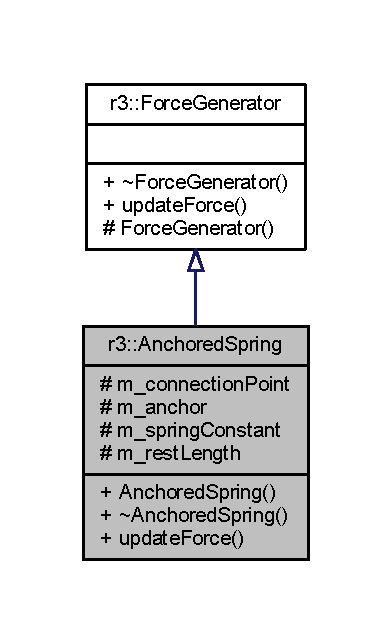
\includegraphics[width=188pt]{classr3_1_1_anchored_spring__inherit__graph}
\end{center}
\end{figure}


Collaboration diagram for r3\+:\+:Anchored\+Spring\+:\nopagebreak
\begin{figure}[H]
\begin{center}
\leavevmode
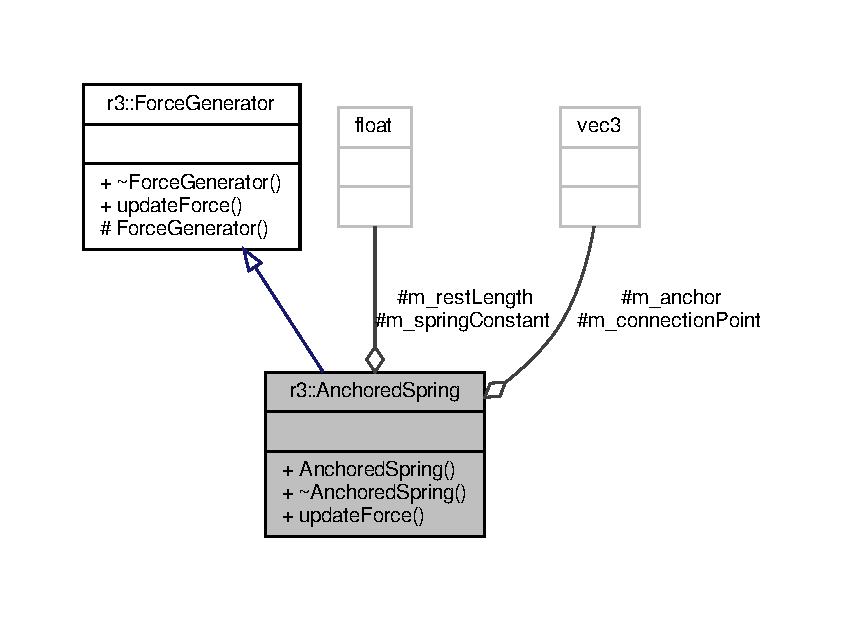
\includegraphics[width=350pt]{classr3_1_1_anchored_spring__coll__graph}
\end{center}
\end{figure}
\subsection*{Public Member Functions}
\begin{DoxyCompactItemize}
\item 
\mbox{\hyperlink{classr3_1_1_anchored_spring_a944423598dfb2e3f080f9f9850c8aa13}{Anchored\+Spring}} (const glm\+::vec3 \&anchor, const glm\+::vec3 \&local\+Connection\+Point, \mbox{\hyperlink{namespacer3_ab2016b3e3f743fb735afce242f0dc1eb}{real}} spring\+Constant, \mbox{\hyperlink{namespacer3_ab2016b3e3f743fb735afce242f0dc1eb}{real}} rest\+Length)
\begin{DoxyCompactList}\small\item\em \mbox{\hyperlink{classr3_1_1_anchored_spring}{Anchored\+Spring}} generator. \end{DoxyCompactList}\item 
\mbox{\hyperlink{classr3_1_1_anchored_spring_afe612722d8ed0d7a6f0058dcc21eb17f}{$\sim$\+Anchored\+Spring}} ()
\item 
void \mbox{\hyperlink{classr3_1_1_anchored_spring_a56aaf13c1f89f2b45b6cb95bf16a2300}{update\+Force}} (\mbox{\hyperlink{classr3_1_1_rigid_body}{Rigid\+Body}} $\ast$body) override
\begin{DoxyCompactList}\small\item\em Apply force to a rigid body over a specific time. \end{DoxyCompactList}\end{DoxyCompactItemize}
\subsection*{Protected Attributes}
\begin{DoxyCompactItemize}
\item 
glm\+::vec3 \mbox{\hyperlink{classr3_1_1_anchored_spring_ac8998ca820fd075aed011136155ec1fb}{m\+\_\+connection\+Point}}
\item 
glm\+::vec3 \mbox{\hyperlink{classr3_1_1_anchored_spring_a1387aec403f6955848fe8c3a28b90a9e}{m\+\_\+anchor}}
\item 
\mbox{\hyperlink{namespacer3_ab2016b3e3f743fb735afce242f0dc1eb}{real}} \mbox{\hyperlink{classr3_1_1_anchored_spring_af17c024b5f8a025f5555946c60b52a67}{m\+\_\+spring\+Constant}}
\item 
\mbox{\hyperlink{namespacer3_ab2016b3e3f743fb735afce242f0dc1eb}{real}} \mbox{\hyperlink{classr3_1_1_anchored_spring_a17441401eb79dd8244a4739a3a574d1a}{m\+\_\+rest\+Length}}
\end{DoxyCompactItemize}
\subsection*{Additional Inherited Members}


\subsection{Detailed Description}
An \mbox{\hyperlink{classr3_1_1_anchored_spring}{Anchored\+Spring}} is a force generator that simulates spring forces. 

One end of the spring is a static point. 

\subsection{Constructor \& Destructor Documentation}
\mbox{\Hypertarget{classr3_1_1_anchored_spring_a944423598dfb2e3f080f9f9850c8aa13}\label{classr3_1_1_anchored_spring_a944423598dfb2e3f080f9f9850c8aa13}} 
\index{r3\+::\+Anchored\+Spring@{r3\+::\+Anchored\+Spring}!Anchored\+Spring@{Anchored\+Spring}}
\index{Anchored\+Spring@{Anchored\+Spring}!r3\+::\+Anchored\+Spring@{r3\+::\+Anchored\+Spring}}
\subsubsection{\texorpdfstring{Anchored\+Spring()}{AnchoredSpring()}}
{\footnotesize\ttfamily r3\+::\+Anchored\+Spring\+::\+Anchored\+Spring (\begin{DoxyParamCaption}\item[{const glm\+::vec3 \&}]{anchor,  }\item[{const glm\+::vec3 \&}]{local\+Connection\+Point,  }\item[{\mbox{\hyperlink{namespacer3_ab2016b3e3f743fb735afce242f0dc1eb}{real}}}]{spring\+Constant,  }\item[{\mbox{\hyperlink{namespacer3_ab2016b3e3f743fb735afce242f0dc1eb}{real}}}]{rest\+Length }\end{DoxyParamCaption})\hspace{0.3cm}{\ttfamily [explicit]}}



\mbox{\hyperlink{classr3_1_1_anchored_spring}{Anchored\+Spring}} generator. 


\begin{DoxyParams}{Parameters}
{\em anchor} & The static end of the spring in world coordinates. \\
\hline
{\em local\+Connection\+Point} & Connection point of the rigid body (in local coordinates of said body). \\
\hline
{\em spring\+Constant} & The hardness of the spring. \\
\hline
{\em rest\+Length} & The distance at which no forces act. \\
\hline
\end{DoxyParams}
\mbox{\Hypertarget{classr3_1_1_anchored_spring_afe612722d8ed0d7a6f0058dcc21eb17f}\label{classr3_1_1_anchored_spring_afe612722d8ed0d7a6f0058dcc21eb17f}} 
\index{r3\+::\+Anchored\+Spring@{r3\+::\+Anchored\+Spring}!````~Anchored\+Spring@{$\sim$\+Anchored\+Spring}}
\index{````~Anchored\+Spring@{$\sim$\+Anchored\+Spring}!r3\+::\+Anchored\+Spring@{r3\+::\+Anchored\+Spring}}
\subsubsection{\texorpdfstring{$\sim$\+Anchored\+Spring()}{~AnchoredSpring()}}
{\footnotesize\ttfamily r3\+::\+Anchored\+Spring\+::$\sim$\+Anchored\+Spring (\begin{DoxyParamCaption}{ }\end{DoxyParamCaption})\hspace{0.3cm}{\ttfamily [default]}}



\subsection{Member Function Documentation}
\mbox{\Hypertarget{classr3_1_1_anchored_spring_a56aaf13c1f89f2b45b6cb95bf16a2300}\label{classr3_1_1_anchored_spring_a56aaf13c1f89f2b45b6cb95bf16a2300}} 
\index{r3\+::\+Anchored\+Spring@{r3\+::\+Anchored\+Spring}!update\+Force@{update\+Force}}
\index{update\+Force@{update\+Force}!r3\+::\+Anchored\+Spring@{r3\+::\+Anchored\+Spring}}
\subsubsection{\texorpdfstring{update\+Force()}{updateForce()}}
{\footnotesize\ttfamily void r3\+::\+Anchored\+Spring\+::update\+Force (\begin{DoxyParamCaption}\item[{\mbox{\hyperlink{classr3_1_1_rigid_body}{Rigid\+Body}} $\ast$}]{body }\end{DoxyParamCaption})\hspace{0.3cm}{\ttfamily [override]}, {\ttfamily [virtual]}}



Apply force to a rigid body over a specific time. 


\begin{DoxyParams}{Parameters}
{\em body} & The rigid body on which to apply force. \\
\hline
\end{DoxyParams}


Implements \mbox{\hyperlink{classr3_1_1_force_generator_a59deb54721cdcc6e33fabfb1f9a3fb27}{r3\+::\+Force\+Generator}}.



\subsection{Member Data Documentation}
\mbox{\Hypertarget{classr3_1_1_anchored_spring_a1387aec403f6955848fe8c3a28b90a9e}\label{classr3_1_1_anchored_spring_a1387aec403f6955848fe8c3a28b90a9e}} 
\index{r3\+::\+Anchored\+Spring@{r3\+::\+Anchored\+Spring}!m\+\_\+anchor@{m\+\_\+anchor}}
\index{m\+\_\+anchor@{m\+\_\+anchor}!r3\+::\+Anchored\+Spring@{r3\+::\+Anchored\+Spring}}
\subsubsection{\texorpdfstring{m\+\_\+anchor}{m\_anchor}}
{\footnotesize\ttfamily glm\+::vec3 r3\+::\+Anchored\+Spring\+::m\+\_\+anchor\hspace{0.3cm}{\ttfamily [protected]}}

\mbox{\Hypertarget{classr3_1_1_anchored_spring_ac8998ca820fd075aed011136155ec1fb}\label{classr3_1_1_anchored_spring_ac8998ca820fd075aed011136155ec1fb}} 
\index{r3\+::\+Anchored\+Spring@{r3\+::\+Anchored\+Spring}!m\+\_\+connection\+Point@{m\+\_\+connection\+Point}}
\index{m\+\_\+connection\+Point@{m\+\_\+connection\+Point}!r3\+::\+Anchored\+Spring@{r3\+::\+Anchored\+Spring}}
\subsubsection{\texorpdfstring{m\+\_\+connection\+Point}{m\_connectionPoint}}
{\footnotesize\ttfamily glm\+::vec3 r3\+::\+Anchored\+Spring\+::m\+\_\+connection\+Point\hspace{0.3cm}{\ttfamily [protected]}}

\mbox{\Hypertarget{classr3_1_1_anchored_spring_a17441401eb79dd8244a4739a3a574d1a}\label{classr3_1_1_anchored_spring_a17441401eb79dd8244a4739a3a574d1a}} 
\index{r3\+::\+Anchored\+Spring@{r3\+::\+Anchored\+Spring}!m\+\_\+rest\+Length@{m\+\_\+rest\+Length}}
\index{m\+\_\+rest\+Length@{m\+\_\+rest\+Length}!r3\+::\+Anchored\+Spring@{r3\+::\+Anchored\+Spring}}
\subsubsection{\texorpdfstring{m\+\_\+rest\+Length}{m\_restLength}}
{\footnotesize\ttfamily \mbox{\hyperlink{namespacer3_ab2016b3e3f743fb735afce242f0dc1eb}{real}} r3\+::\+Anchored\+Spring\+::m\+\_\+rest\+Length\hspace{0.3cm}{\ttfamily [protected]}}

\mbox{\Hypertarget{classr3_1_1_anchored_spring_af17c024b5f8a025f5555946c60b52a67}\label{classr3_1_1_anchored_spring_af17c024b5f8a025f5555946c60b52a67}} 
\index{r3\+::\+Anchored\+Spring@{r3\+::\+Anchored\+Spring}!m\+\_\+spring\+Constant@{m\+\_\+spring\+Constant}}
\index{m\+\_\+spring\+Constant@{m\+\_\+spring\+Constant}!r3\+::\+Anchored\+Spring@{r3\+::\+Anchored\+Spring}}
\subsubsection{\texorpdfstring{m\+\_\+spring\+Constant}{m\_springConstant}}
{\footnotesize\ttfamily \mbox{\hyperlink{namespacer3_ab2016b3e3f743fb735afce242f0dc1eb}{real}} r3\+::\+Anchored\+Spring\+::m\+\_\+spring\+Constant\hspace{0.3cm}{\ttfamily [protected]}}



The documentation for this class was generated from the following files\+:\begin{DoxyCompactItemize}
\item 
D\+:/\+Programming/\+Repositories/\+Game\+Physics/\+Simulation\+Visualization/\+Rumble3\+D/\+Rumble3\+D/include/\+R3\+D/\+Rigid\+Body\+Engine/\mbox{\hyperlink{_anchored_spring_8h}{Anchored\+Spring.\+h}}\item 
D\+:/\+Programming/\+Repositories/\+Game\+Physics/\+Simulation\+Visualization/\+Rumble3\+D/\+Rumble3\+D/src/\+Rigid\+Body\+Engine/\mbox{\hyperlink{_anchored_spring_8cpp}{Anchored\+Spring.\+cpp}}\end{DoxyCompactItemize}

\hypertarget{classr3_1_1_bounding_box}{}\doxysection{r3\+::Bounding\+Box Class Reference}
\label{classr3_1_1_bounding_box}\index{r3::BoundingBox@{r3::BoundingBox}}


{\ttfamily \#include $<$Bounding\+Box.\+h$>$}



Collaboration diagram for r3\+::Bounding\+Box\+:\nopagebreak
\begin{figure}[H]
\begin{center}
\leavevmode
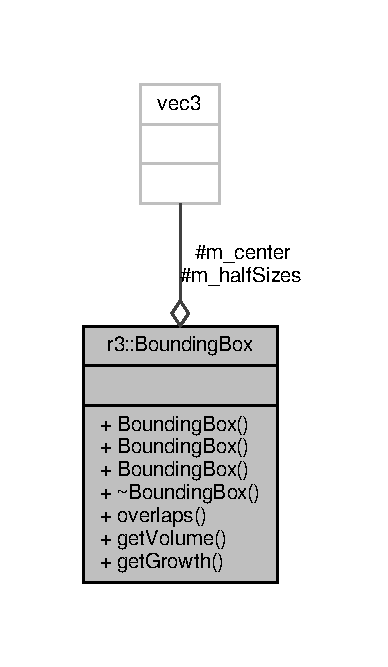
\includegraphics[width=186pt]{classr3_1_1_bounding_box__coll__graph}
\end{center}
\end{figure}
\doxysubsection*{Public Member Functions}
\begin{DoxyCompactItemize}
\item 
\mbox{\hyperlink{classr3_1_1_bounding_box_a088852419e2b7af17f2e94d672a70bcf}{Bounding\+Box}} ()
\item 
\mbox{\hyperlink{classr3_1_1_bounding_box_a871e0ce668df300a9a88eef1069d1874}{Bounding\+Box}} (const glm\+::vec3 \&center, const glm\+::vec3 \&half\+Sizes)
\begin{DoxyCompactList}\small\item\em \mbox{\hyperlink{classr3_1_1_bounding_box}{Bounding\+Box}} constructor. \end{DoxyCompactList}\item 
\mbox{\hyperlink{classr3_1_1_bounding_box_a23750f8e74b918e0b39ce2c2fe609574}{Bounding\+Box}} (const \mbox{\hyperlink{classr3_1_1_bounding_box}{Bounding\+Box}} \&one, const \mbox{\hyperlink{classr3_1_1_bounding_box}{Bounding\+Box}} \&two)
\begin{DoxyCompactList}\small\item\em \mbox{\hyperlink{classr3_1_1_bounding_box}{Bounding\+Box}} constructor. Create a bounding box which contains both given boxes. \end{DoxyCompactList}\item 
\mbox{\hyperlink{classr3_1_1_bounding_box_a9257cfab936d3331cba765cb19527aa1}{$\sim$\+Bounding\+Box}} ()
\item 
bool \mbox{\hyperlink{classr3_1_1_bounding_box_a6e69163febe125531fa355ae9876b8be}{overlaps}} (const \mbox{\hyperlink{classr3_1_1_bounding_box}{Bounding\+Box}} $\ast$other) const
\begin{DoxyCompactList}\small\item\em Check the given bounding box overlaps with this one. \end{DoxyCompactList}\item 
\mbox{\hyperlink{namespacer3_ab2016b3e3f743fb735afce242f0dc1eb}{real}} \mbox{\hyperlink{classr3_1_1_bounding_box_a3e6a9b79373dde150d18d5d5df59a2f3}{get\+Volume}} () const
\begin{DoxyCompactList}\small\item\em Get the volume of this bounding box. \end{DoxyCompactList}\item 
\mbox{\hyperlink{namespacer3_ab2016b3e3f743fb735afce242f0dc1eb}{real}} \mbox{\hyperlink{classr3_1_1_bounding_box_a21631e2fffeb995d3a9647489f936d13}{get\+Growth}} (const \mbox{\hyperlink{classr3_1_1_bounding_box}{Bounding\+Box}} \&other) const
\begin{DoxyCompactList}\small\item\em Get an approximation of how much a new bounding box, including the given and this one, would be relatively to this one. \end{DoxyCompactList}\end{DoxyCompactItemize}
\doxysubsection*{Protected Attributes}
\begin{DoxyCompactItemize}
\item 
glm\+::vec3 \mbox{\hyperlink{classr3_1_1_bounding_box_ae7f47ade2f27fb7e76da58c944141d80}{m\+\_\+center}}
\item 
glm\+::vec3 \mbox{\hyperlink{classr3_1_1_bounding_box_ac95d88875ec61c04133186507bc613dc}{m\+\_\+half\+Sizes}}
\end{DoxyCompactItemize}


\doxysubsection{Constructor \& Destructor Documentation}
\mbox{\Hypertarget{classr3_1_1_bounding_box_a088852419e2b7af17f2e94d672a70bcf}\label{classr3_1_1_bounding_box_a088852419e2b7af17f2e94d672a70bcf}} 
\index{r3::BoundingBox@{r3::BoundingBox}!BoundingBox@{BoundingBox}}
\index{BoundingBox@{BoundingBox}!r3::BoundingBox@{r3::BoundingBox}}
\doxysubsubsection{\texorpdfstring{BoundingBox()}{BoundingBox()}\hspace{0.1cm}{\footnotesize\ttfamily [1/3]}}
{\footnotesize\ttfamily r3\+::\+Bounding\+Box\+::\+Bounding\+Box (\begin{DoxyParamCaption}{ }\end{DoxyParamCaption})}

\mbox{\Hypertarget{classr3_1_1_bounding_box_a871e0ce668df300a9a88eef1069d1874}\label{classr3_1_1_bounding_box_a871e0ce668df300a9a88eef1069d1874}} 
\index{r3::BoundingBox@{r3::BoundingBox}!BoundingBox@{BoundingBox}}
\index{BoundingBox@{BoundingBox}!r3::BoundingBox@{r3::BoundingBox}}
\doxysubsubsection{\texorpdfstring{BoundingBox()}{BoundingBox()}\hspace{0.1cm}{\footnotesize\ttfamily [2/3]}}
{\footnotesize\ttfamily r3\+::\+Bounding\+Box\+::\+Bounding\+Box (\begin{DoxyParamCaption}\item[{const glm\+::vec3 \&}]{center,  }\item[{const glm\+::vec3 \&}]{half\+Sizes }\end{DoxyParamCaption})}



\mbox{\hyperlink{classr3_1_1_bounding_box}{Bounding\+Box}} constructor. 


\begin{DoxyParams}{Parameters}
{\em center} & The center of the box in world coordinates. \\
\hline
{\em bounds} & Half sizes of the box. \\
\hline
\end{DoxyParams}
\mbox{\Hypertarget{classr3_1_1_bounding_box_a23750f8e74b918e0b39ce2c2fe609574}\label{classr3_1_1_bounding_box_a23750f8e74b918e0b39ce2c2fe609574}} 
\index{r3::BoundingBox@{r3::BoundingBox}!BoundingBox@{BoundingBox}}
\index{BoundingBox@{BoundingBox}!r3::BoundingBox@{r3::BoundingBox}}
\doxysubsubsection{\texorpdfstring{BoundingBox()}{BoundingBox()}\hspace{0.1cm}{\footnotesize\ttfamily [3/3]}}
{\footnotesize\ttfamily r3\+::\+Bounding\+Box\+::\+Bounding\+Box (\begin{DoxyParamCaption}\item[{const \mbox{\hyperlink{classr3_1_1_bounding_box}{Bounding\+Box}} \&}]{one,  }\item[{const \mbox{\hyperlink{classr3_1_1_bounding_box}{Bounding\+Box}} \&}]{two }\end{DoxyParamCaption})}



\mbox{\hyperlink{classr3_1_1_bounding_box}{Bounding\+Box}} constructor. Create a bounding box which contains both given boxes. 


\begin{DoxyParams}{Parameters}
{\em one} & The first contained bounding box. \\
\hline
{\em two} & The second contained bounding box. \\
\hline
\end{DoxyParams}
\mbox{\Hypertarget{classr3_1_1_bounding_box_a9257cfab936d3331cba765cb19527aa1}\label{classr3_1_1_bounding_box_a9257cfab936d3331cba765cb19527aa1}} 
\index{r3::BoundingBox@{r3::BoundingBox}!````~BoundingBox@{$\sim$BoundingBox}}
\index{````~BoundingBox@{$\sim$BoundingBox}!r3::BoundingBox@{r3::BoundingBox}}
\doxysubsubsection{\texorpdfstring{$\sim$BoundingBox()}{~BoundingBox()}}
{\footnotesize\ttfamily r3\+::\+Bounding\+Box\+::$\sim$\+Bounding\+Box (\begin{DoxyParamCaption}{ }\end{DoxyParamCaption})\hspace{0.3cm}{\ttfamily [default]}}



\doxysubsection{Member Function Documentation}
\mbox{\Hypertarget{classr3_1_1_bounding_box_a21631e2fffeb995d3a9647489f936d13}\label{classr3_1_1_bounding_box_a21631e2fffeb995d3a9647489f936d13}} 
\index{r3::BoundingBox@{r3::BoundingBox}!getGrowth@{getGrowth}}
\index{getGrowth@{getGrowth}!r3::BoundingBox@{r3::BoundingBox}}
\doxysubsubsection{\texorpdfstring{getGrowth()}{getGrowth()}}
{\footnotesize\ttfamily \mbox{\hyperlink{namespacer3_ab2016b3e3f743fb735afce242f0dc1eb}{real}} r3\+::\+Bounding\+Box\+::get\+Growth (\begin{DoxyParamCaption}\item[{const \mbox{\hyperlink{classr3_1_1_bounding_box}{Bounding\+Box}} \&}]{other }\end{DoxyParamCaption}) const}



Get an approximation of how much a new bounding box, including the given and this one, would be relatively to this one. 


\begin{DoxyParams}{Parameters}
{\em other} & The added volume. \\
\hline
\end{DoxyParams}
\begin{DoxyReturn}{Returns}
The growth. 
\end{DoxyReturn}
\mbox{\Hypertarget{classr3_1_1_bounding_box_a3e6a9b79373dde150d18d5d5df59a2f3}\label{classr3_1_1_bounding_box_a3e6a9b79373dde150d18d5d5df59a2f3}} 
\index{r3::BoundingBox@{r3::BoundingBox}!getVolume@{getVolume}}
\index{getVolume@{getVolume}!r3::BoundingBox@{r3::BoundingBox}}
\doxysubsubsection{\texorpdfstring{getVolume()}{getVolume()}}
{\footnotesize\ttfamily \mbox{\hyperlink{namespacer3_ab2016b3e3f743fb735afce242f0dc1eb}{real}} r3\+::\+Bounding\+Box\+::get\+Volume (\begin{DoxyParamCaption}{ }\end{DoxyParamCaption}) const}



Get the volume of this bounding box. 

\begin{DoxyReturn}{Returns}
The volume. 
\end{DoxyReturn}
\mbox{\Hypertarget{classr3_1_1_bounding_box_a6e69163febe125531fa355ae9876b8be}\label{classr3_1_1_bounding_box_a6e69163febe125531fa355ae9876b8be}} 
\index{r3::BoundingBox@{r3::BoundingBox}!overlaps@{overlaps}}
\index{overlaps@{overlaps}!r3::BoundingBox@{r3::BoundingBox}}
\doxysubsubsection{\texorpdfstring{overlaps()}{overlaps()}}
{\footnotesize\ttfamily bool r3\+::\+Bounding\+Box\+::overlaps (\begin{DoxyParamCaption}\item[{const \mbox{\hyperlink{classr3_1_1_bounding_box}{Bounding\+Box}} $\ast$}]{other }\end{DoxyParamCaption}) const}



Check the given bounding box overlaps with this one. 


\begin{DoxyParams}{Parameters}
{\em other} & The other bounding box to check against. \\
\hline
\end{DoxyParams}
\begin{DoxyReturn}{Returns}
True if there is a collision, false otherwise. 
\end{DoxyReturn}


\doxysubsection{Member Data Documentation}
\mbox{\Hypertarget{classr3_1_1_bounding_box_ae7f47ade2f27fb7e76da58c944141d80}\label{classr3_1_1_bounding_box_ae7f47ade2f27fb7e76da58c944141d80}} 
\index{r3::BoundingBox@{r3::BoundingBox}!m\_center@{m\_center}}
\index{m\_center@{m\_center}!r3::BoundingBox@{r3::BoundingBox}}
\doxysubsubsection{\texorpdfstring{m\_center}{m\_center}}
{\footnotesize\ttfamily glm\+::vec3 r3\+::\+Bounding\+Box\+::m\+\_\+center\hspace{0.3cm}{\ttfamily [protected]}}

\mbox{\Hypertarget{classr3_1_1_bounding_box_ac95d88875ec61c04133186507bc613dc}\label{classr3_1_1_bounding_box_ac95d88875ec61c04133186507bc613dc}} 
\index{r3::BoundingBox@{r3::BoundingBox}!m\_halfSizes@{m\_halfSizes}}
\index{m\_halfSizes@{m\_halfSizes}!r3::BoundingBox@{r3::BoundingBox}}
\doxysubsubsection{\texorpdfstring{m\_halfSizes}{m\_halfSizes}}
{\footnotesize\ttfamily glm\+::vec3 r3\+::\+Bounding\+Box\+::m\+\_\+half\+Sizes\hspace{0.3cm}{\ttfamily [protected]}}



The documentation for this class was generated from the following files\+:\begin{DoxyCompactItemize}
\item 
/home/nelaty/\+Development/\+Repositories/\+Rumble3\+D/include/\+R3\+D/\+Rigid\+Body\+Engine/\mbox{\hyperlink{_bounding_box_8h}{Bounding\+Box.\+h}}\item 
/home/nelaty/\+Development/\+Repositories/\+Rumble3\+D/src/\+Rigid\+Body\+Engine/\mbox{\hyperlink{_bounding_box_8cpp}{Bounding\+Box.\+cpp}}\end{DoxyCompactItemize}

\hypertarget{classr3_1_1_bounding_sphere}{}\doxysection{r3\+::Bounding\+Sphere Class Reference}
\label{classr3_1_1_bounding_sphere}\index{r3::BoundingSphere@{r3::BoundingSphere}}


A bounding sphere is a kind of bounding volume.  




{\ttfamily \#include $<$Bounding\+Sphere.\+h$>$}



Collaboration diagram for r3\+::Bounding\+Sphere\+:\nopagebreak
\begin{figure}[H]
\begin{center}
\leavevmode
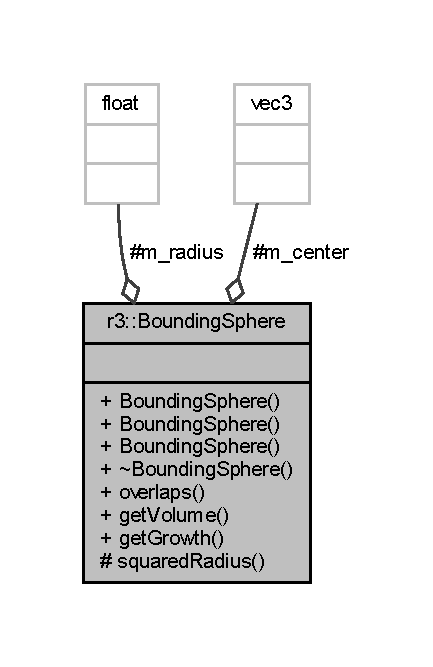
\includegraphics[width=206pt]{classr3_1_1_bounding_sphere__coll__graph}
\end{center}
\end{figure}
\doxysubsection*{Public Member Functions}
\begin{DoxyCompactItemize}
\item 
\mbox{\hyperlink{classr3_1_1_bounding_sphere_af602a853d8ed0b5ccad8679ee41fe7f8}{Bounding\+Sphere}} ()
\item 
\mbox{\hyperlink{classr3_1_1_bounding_sphere_a9a9264c19d56b10c9b0def547a369d57}{Bounding\+Sphere}} (const glm\+::vec3 \&center, \mbox{\hyperlink{namespacer3_ab2016b3e3f743fb735afce242f0dc1eb}{real}} radius)
\begin{DoxyCompactList}\small\item\em \mbox{\hyperlink{classr3_1_1_bounding_box}{Bounding\+Box}} constructor. \end{DoxyCompactList}\item 
\mbox{\hyperlink{classr3_1_1_bounding_sphere_a3d461e62b827ad9a30ca8013d451e3da}{Bounding\+Sphere}} (const \mbox{\hyperlink{classr3_1_1_bounding_sphere}{Bounding\+Sphere}} \&one, const \mbox{\hyperlink{classr3_1_1_bounding_sphere}{Bounding\+Sphere}} \&two)
\begin{DoxyCompactList}\small\item\em \mbox{\hyperlink{classr3_1_1_bounding_sphere}{Bounding\+Sphere}} constructor. \end{DoxyCompactList}\item 
\mbox{\hyperlink{classr3_1_1_bounding_sphere_a9951f8922ebb2227cd97e59c97fed2a5}{$\sim$\+Bounding\+Sphere}} ()
\item 
bool \mbox{\hyperlink{classr3_1_1_bounding_sphere_a49163c78b0d1318c576d99e61f806ac2}{overlaps}} (const \mbox{\hyperlink{classr3_1_1_bounding_sphere}{Bounding\+Sphere}} $\ast$other) const
\begin{DoxyCompactList}\small\item\em Check if this bounding sphere overlaps with the given bounding sphere. \end{DoxyCompactList}\item 
\mbox{\hyperlink{namespacer3_ab2016b3e3f743fb735afce242f0dc1eb}{real}} \mbox{\hyperlink{classr3_1_1_bounding_sphere_a01cc1a7397eeec86d2b074d2bf734798}{get\+Volume}} () const
\item 
\mbox{\hyperlink{namespacer3_ab2016b3e3f743fb735afce242f0dc1eb}{real}} \mbox{\hyperlink{classr3_1_1_bounding_sphere_ac13a86be56c1c52b33a707eb2356daa3}{get\+Growth}} (const \mbox{\hyperlink{classr3_1_1_bounding_sphere}{Bounding\+Sphere}} \&other) const
\begin{DoxyCompactList}\small\item\em Get an approximation of how much a new bounding sphere, including the given and this one, would be relatively to this one. \end{DoxyCompactList}\end{DoxyCompactItemize}
\doxysubsection*{Protected Member Functions}
\begin{DoxyCompactItemize}
\item 
\mbox{\hyperlink{namespacer3_ab2016b3e3f743fb735afce242f0dc1eb}{real}} \mbox{\hyperlink{classr3_1_1_bounding_sphere_ae0e7a71b8cfe2f3287397ac865545ee4}{squared\+Radius}} () const
\begin{DoxyCompactList}\small\item\em Calculate the square of this spheres radius. \end{DoxyCompactList}\end{DoxyCompactItemize}
\doxysubsection*{Protected Attributes}
\begin{DoxyCompactItemize}
\item 
glm\+::vec3 \mbox{\hyperlink{classr3_1_1_bounding_sphere_a880d9888f25b016c5c38c608e16fa61e}{m\+\_\+center}}
\item 
\mbox{\hyperlink{namespacer3_ab2016b3e3f743fb735afce242f0dc1eb}{real}} \mbox{\hyperlink{classr3_1_1_bounding_sphere_a37ccefd38d8cea7a0d52b85f771ec7c4}{m\+\_\+radius}} \{\}
\end{DoxyCompactItemize}


\doxysubsection{Detailed Description}
A bounding sphere is a kind of bounding volume. 

\doxysubsection{Constructor \& Destructor Documentation}
\mbox{\Hypertarget{classr3_1_1_bounding_sphere_af602a853d8ed0b5ccad8679ee41fe7f8}\label{classr3_1_1_bounding_sphere_af602a853d8ed0b5ccad8679ee41fe7f8}} 
\index{r3::BoundingSphere@{r3::BoundingSphere}!BoundingSphere@{BoundingSphere}}
\index{BoundingSphere@{BoundingSphere}!r3::BoundingSphere@{r3::BoundingSphere}}
\doxysubsubsection{\texorpdfstring{BoundingSphere()}{BoundingSphere()}\hspace{0.1cm}{\footnotesize\ttfamily [1/3]}}
{\footnotesize\ttfamily r3\+::\+Bounding\+Sphere\+::\+Bounding\+Sphere (\begin{DoxyParamCaption}{ }\end{DoxyParamCaption})\hspace{0.3cm}{\ttfamily [default]}}

\mbox{\Hypertarget{classr3_1_1_bounding_sphere_a9a9264c19d56b10c9b0def547a369d57}\label{classr3_1_1_bounding_sphere_a9a9264c19d56b10c9b0def547a369d57}} 
\index{r3::BoundingSphere@{r3::BoundingSphere}!BoundingSphere@{BoundingSphere}}
\index{BoundingSphere@{BoundingSphere}!r3::BoundingSphere@{r3::BoundingSphere}}
\doxysubsubsection{\texorpdfstring{BoundingSphere()}{BoundingSphere()}\hspace{0.1cm}{\footnotesize\ttfamily [2/3]}}
{\footnotesize\ttfamily r3\+::\+Bounding\+Sphere\+::\+Bounding\+Sphere (\begin{DoxyParamCaption}\item[{const glm\+::vec3 \&}]{center,  }\item[{\mbox{\hyperlink{namespacer3_ab2016b3e3f743fb735afce242f0dc1eb}{real}}}]{radius }\end{DoxyParamCaption})}



\mbox{\hyperlink{classr3_1_1_bounding_box}{Bounding\+Box}} constructor. 


\begin{DoxyParams}{Parameters}
{\em center} & The center of the spehere in world coordinates. \\
\hline
{\em radius} & The radius of the sphere \\
\hline
\end{DoxyParams}
\mbox{\Hypertarget{classr3_1_1_bounding_sphere_a3d461e62b827ad9a30ca8013d451e3da}\label{classr3_1_1_bounding_sphere_a3d461e62b827ad9a30ca8013d451e3da}} 
\index{r3::BoundingSphere@{r3::BoundingSphere}!BoundingSphere@{BoundingSphere}}
\index{BoundingSphere@{BoundingSphere}!r3::BoundingSphere@{r3::BoundingSphere}}
\doxysubsubsection{\texorpdfstring{BoundingSphere()}{BoundingSphere()}\hspace{0.1cm}{\footnotesize\ttfamily [3/3]}}
{\footnotesize\ttfamily r3\+::\+Bounding\+Sphere\+::\+Bounding\+Sphere (\begin{DoxyParamCaption}\item[{const \mbox{\hyperlink{classr3_1_1_bounding_sphere}{Bounding\+Sphere}} \&}]{one,  }\item[{const \mbox{\hyperlink{classr3_1_1_bounding_sphere}{Bounding\+Sphere}} \&}]{two }\end{DoxyParamCaption})}



\mbox{\hyperlink{classr3_1_1_bounding_sphere}{Bounding\+Sphere}} constructor. 

Create a bounding sphere which contains both given spheres. 
\begin{DoxyParams}{Parameters}
{\em one} & The first child bounding sphere. \\
\hline
{\em two} & The second child bounding sphere. \\
\hline
\end{DoxyParams}
\mbox{\Hypertarget{classr3_1_1_bounding_sphere_a9951f8922ebb2227cd97e59c97fed2a5}\label{classr3_1_1_bounding_sphere_a9951f8922ebb2227cd97e59c97fed2a5}} 
\index{r3::BoundingSphere@{r3::BoundingSphere}!````~BoundingSphere@{$\sim$BoundingSphere}}
\index{````~BoundingSphere@{$\sim$BoundingSphere}!r3::BoundingSphere@{r3::BoundingSphere}}
\doxysubsubsection{\texorpdfstring{$\sim$BoundingSphere()}{~BoundingSphere()}}
{\footnotesize\ttfamily r3\+::\+Bounding\+Sphere\+::$\sim$\+Bounding\+Sphere (\begin{DoxyParamCaption}{ }\end{DoxyParamCaption})\hspace{0.3cm}{\ttfamily [default]}}



\doxysubsection{Member Function Documentation}
\mbox{\Hypertarget{classr3_1_1_bounding_sphere_ac13a86be56c1c52b33a707eb2356daa3}\label{classr3_1_1_bounding_sphere_ac13a86be56c1c52b33a707eb2356daa3}} 
\index{r3::BoundingSphere@{r3::BoundingSphere}!getGrowth@{getGrowth}}
\index{getGrowth@{getGrowth}!r3::BoundingSphere@{r3::BoundingSphere}}
\doxysubsubsection{\texorpdfstring{getGrowth()}{getGrowth()}}
{\footnotesize\ttfamily \mbox{\hyperlink{namespacer3_ab2016b3e3f743fb735afce242f0dc1eb}{real}} r3\+::\+Bounding\+Sphere\+::get\+Growth (\begin{DoxyParamCaption}\item[{const \mbox{\hyperlink{classr3_1_1_bounding_sphere}{Bounding\+Sphere}} \&}]{other }\end{DoxyParamCaption}) const}



Get an approximation of how much a new bounding sphere, including the given and this one, would be relatively to this one. 


\begin{DoxyParams}{Parameters}
{\em other} & The added volume. \\
\hline
\end{DoxyParams}
\begin{DoxyReturn}{Returns}
The growth. 
\end{DoxyReturn}
\mbox{\Hypertarget{classr3_1_1_bounding_sphere_a01cc1a7397eeec86d2b074d2bf734798}\label{classr3_1_1_bounding_sphere_a01cc1a7397eeec86d2b074d2bf734798}} 
\index{r3::BoundingSphere@{r3::BoundingSphere}!getVolume@{getVolume}}
\index{getVolume@{getVolume}!r3::BoundingSphere@{r3::BoundingSphere}}
\doxysubsubsection{\texorpdfstring{getVolume()}{getVolume()}}
{\footnotesize\ttfamily \mbox{\hyperlink{namespacer3_ab2016b3e3f743fb735afce242f0dc1eb}{real}} r3\+::\+Bounding\+Sphere\+::get\+Volume (\begin{DoxyParamCaption}{ }\end{DoxyParamCaption}) const}

\textbackslash{}biref Get the volume of this bounding sphere. \begin{DoxyReturn}{Returns}
The volume. 
\end{DoxyReturn}
\mbox{\Hypertarget{classr3_1_1_bounding_sphere_a49163c78b0d1318c576d99e61f806ac2}\label{classr3_1_1_bounding_sphere_a49163c78b0d1318c576d99e61f806ac2}} 
\index{r3::BoundingSphere@{r3::BoundingSphere}!overlaps@{overlaps}}
\index{overlaps@{overlaps}!r3::BoundingSphere@{r3::BoundingSphere}}
\doxysubsubsection{\texorpdfstring{overlaps()}{overlaps()}}
{\footnotesize\ttfamily bool r3\+::\+Bounding\+Sphere\+::overlaps (\begin{DoxyParamCaption}\item[{const \mbox{\hyperlink{classr3_1_1_bounding_sphere}{Bounding\+Sphere}} $\ast$}]{other }\end{DoxyParamCaption}) const}



Check if this bounding sphere overlaps with the given bounding sphere. 

\begin{DoxyReturn}{Returns}
True if they overlap, false otherwise. 
\end{DoxyReturn}
\mbox{\Hypertarget{classr3_1_1_bounding_sphere_ae0e7a71b8cfe2f3287397ac865545ee4}\label{classr3_1_1_bounding_sphere_ae0e7a71b8cfe2f3287397ac865545ee4}} 
\index{r3::BoundingSphere@{r3::BoundingSphere}!squaredRadius@{squaredRadius}}
\index{squaredRadius@{squaredRadius}!r3::BoundingSphere@{r3::BoundingSphere}}
\doxysubsubsection{\texorpdfstring{squaredRadius()}{squaredRadius()}}
{\footnotesize\ttfamily \mbox{\hyperlink{namespacer3_ab2016b3e3f743fb735afce242f0dc1eb}{real}} r3\+::\+Bounding\+Sphere\+::squared\+Radius (\begin{DoxyParamCaption}{ }\end{DoxyParamCaption}) const\hspace{0.3cm}{\ttfamily [protected]}}



Calculate the square of this spheres radius. 

\begin{DoxyReturn}{Returns}
The squared radius. 
\end{DoxyReturn}


\doxysubsection{Member Data Documentation}
\mbox{\Hypertarget{classr3_1_1_bounding_sphere_a880d9888f25b016c5c38c608e16fa61e}\label{classr3_1_1_bounding_sphere_a880d9888f25b016c5c38c608e16fa61e}} 
\index{r3::BoundingSphere@{r3::BoundingSphere}!m\_center@{m\_center}}
\index{m\_center@{m\_center}!r3::BoundingSphere@{r3::BoundingSphere}}
\doxysubsubsection{\texorpdfstring{m\_center}{m\_center}}
{\footnotesize\ttfamily glm\+::vec3 r3\+::\+Bounding\+Sphere\+::m\+\_\+center\hspace{0.3cm}{\ttfamily [protected]}}

\mbox{\Hypertarget{classr3_1_1_bounding_sphere_a37ccefd38d8cea7a0d52b85f771ec7c4}\label{classr3_1_1_bounding_sphere_a37ccefd38d8cea7a0d52b85f771ec7c4}} 
\index{r3::BoundingSphere@{r3::BoundingSphere}!m\_radius@{m\_radius}}
\index{m\_radius@{m\_radius}!r3::BoundingSphere@{r3::BoundingSphere}}
\doxysubsubsection{\texorpdfstring{m\_radius}{m\_radius}}
{\footnotesize\ttfamily \mbox{\hyperlink{namespacer3_ab2016b3e3f743fb735afce242f0dc1eb}{real}} r3\+::\+Bounding\+Sphere\+::m\+\_\+radius \{\}\hspace{0.3cm}{\ttfamily [protected]}}



The documentation for this class was generated from the following files\+:\begin{DoxyCompactItemize}
\item 
/home/nelaty/\+Development/\+Repositories/\+Rumble3\+D/include/\+R3\+D/\+Rigid\+Body\+Engine/\mbox{\hyperlink{_bounding_sphere_8h}{Bounding\+Sphere.\+h}}\item 
/home/nelaty/\+Development/\+Repositories/\+Rumble3\+D/src/\+Rigid\+Body\+Engine/\mbox{\hyperlink{_bounding_sphere_8cpp}{Bounding\+Sphere.\+cpp}}\end{DoxyCompactItemize}

\hypertarget{classr3_1_1_box_box_narrow_algorithm}{}\section{r3\+:\+:Box\+Box\+Narrow\+Algorithm Class Reference}
\label{classr3_1_1_box_box_narrow_algorithm}\index{r3\+::\+Box\+Box\+Narrow\+Algorithm@{r3\+::\+Box\+Box\+Narrow\+Algorithm}}


Default implementation for a box-\/box narrow algorithm.  




{\ttfamily \#include $<$Box\+Box\+Narrow\+Algorithm.\+h$>$}



Inheritance diagram for r3\+:\+:Box\+Box\+Narrow\+Algorithm\+:\nopagebreak
\begin{figure}[H]
\begin{center}
\leavevmode
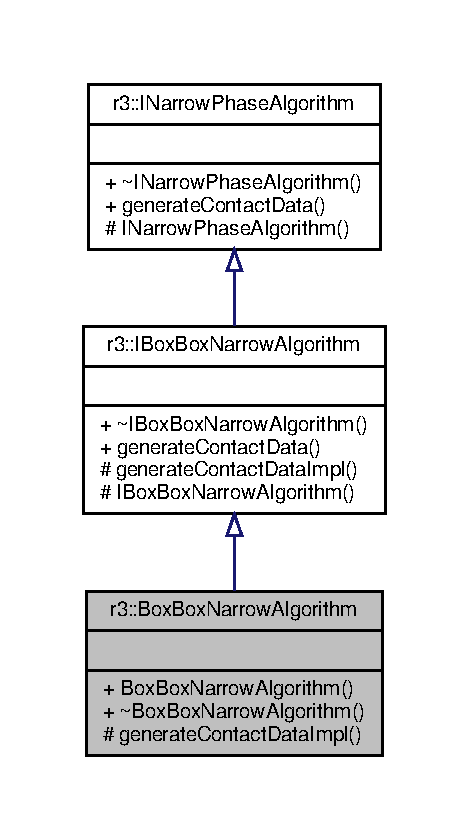
\includegraphics[width=226pt]{classr3_1_1_box_box_narrow_algorithm__inherit__graph}
\end{center}
\end{figure}


Collaboration diagram for r3\+:\+:Box\+Box\+Narrow\+Algorithm\+:\nopagebreak
\begin{figure}[H]
\begin{center}
\leavevmode
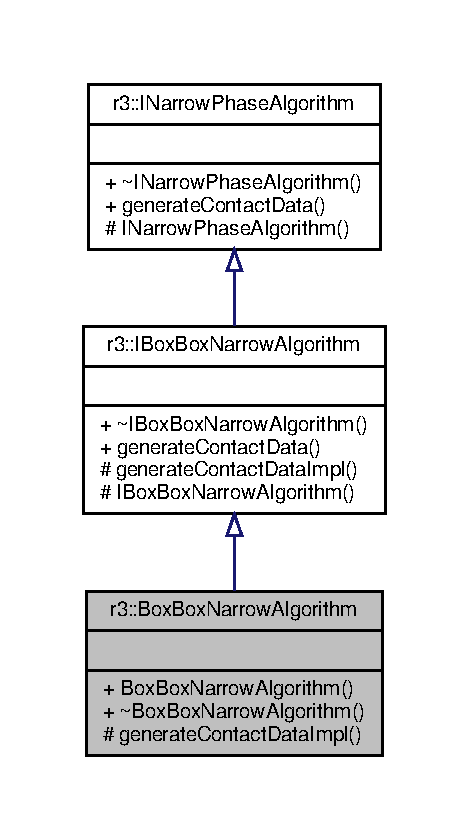
\includegraphics[width=226pt]{classr3_1_1_box_box_narrow_algorithm__coll__graph}
\end{center}
\end{figure}
\subsection*{Public Member Functions}
\begin{DoxyCompactItemize}
\item 
\mbox{\hyperlink{classr3_1_1_box_box_narrow_algorithm_a3c801622b4235a4738d18fef0eda9949}{Box\+Box\+Narrow\+Algorithm}} ()
\item 
\mbox{\hyperlink{classr3_1_1_box_box_narrow_algorithm_a67eb8bd09d7531a5917ac5e720733075}{$\sim$\+Box\+Box\+Narrow\+Algorithm}} ()
\end{DoxyCompactItemize}
\subsection*{Protected Member Functions}
\begin{DoxyCompactItemize}
\item 
bool \mbox{\hyperlink{classr3_1_1_box_box_narrow_algorithm_a200098ad4e6e2381f58856002a2d5dec}{generate\+Contact\+Data\+Impl}} (\mbox{\hyperlink{classr3_1_1_rigid_body}{Rigid\+Body}} $\ast$rb\+Box1, \mbox{\hyperlink{classr3_1_1_collision_box}{Collision\+Box}} $\ast$box1, \mbox{\hyperlink{classr3_1_1_rigid_body}{Rigid\+Body}} $\ast$rb\+Box2, \mbox{\hyperlink{classr3_1_1_collision_box}{Collision\+Box}} $\ast$box2, \mbox{\hyperlink{classr3_1_1_collision_data}{Collision\+Data}} \&collision\+Data) override
\end{DoxyCompactItemize}


\subsection{Detailed Description}
Default implementation for a box-\/box narrow algorithm. 

\subsection{Constructor \& Destructor Documentation}
\mbox{\Hypertarget{classr3_1_1_box_box_narrow_algorithm_a3c801622b4235a4738d18fef0eda9949}\label{classr3_1_1_box_box_narrow_algorithm_a3c801622b4235a4738d18fef0eda9949}} 
\index{r3\+::\+Box\+Box\+Narrow\+Algorithm@{r3\+::\+Box\+Box\+Narrow\+Algorithm}!Box\+Box\+Narrow\+Algorithm@{Box\+Box\+Narrow\+Algorithm}}
\index{Box\+Box\+Narrow\+Algorithm@{Box\+Box\+Narrow\+Algorithm}!r3\+::\+Box\+Box\+Narrow\+Algorithm@{r3\+::\+Box\+Box\+Narrow\+Algorithm}}
\subsubsection{\texorpdfstring{Box\+Box\+Narrow\+Algorithm()}{BoxBoxNarrowAlgorithm()}}
{\footnotesize\ttfamily r3\+::\+Box\+Box\+Narrow\+Algorithm\+::\+Box\+Box\+Narrow\+Algorithm (\begin{DoxyParamCaption}{ }\end{DoxyParamCaption})\hspace{0.3cm}{\ttfamily [explicit]}, {\ttfamily [default]}}

\mbox{\Hypertarget{classr3_1_1_box_box_narrow_algorithm_a67eb8bd09d7531a5917ac5e720733075}\label{classr3_1_1_box_box_narrow_algorithm_a67eb8bd09d7531a5917ac5e720733075}} 
\index{r3\+::\+Box\+Box\+Narrow\+Algorithm@{r3\+::\+Box\+Box\+Narrow\+Algorithm}!````~Box\+Box\+Narrow\+Algorithm@{$\sim$\+Box\+Box\+Narrow\+Algorithm}}
\index{````~Box\+Box\+Narrow\+Algorithm@{$\sim$\+Box\+Box\+Narrow\+Algorithm}!r3\+::\+Box\+Box\+Narrow\+Algorithm@{r3\+::\+Box\+Box\+Narrow\+Algorithm}}
\subsubsection{\texorpdfstring{$\sim$\+Box\+Box\+Narrow\+Algorithm()}{~BoxBoxNarrowAlgorithm()}}
{\footnotesize\ttfamily r3\+::\+Box\+Box\+Narrow\+Algorithm\+::$\sim$\+Box\+Box\+Narrow\+Algorithm (\begin{DoxyParamCaption}{ }\end{DoxyParamCaption})\hspace{0.3cm}{\ttfamily [default]}}



\subsection{Member Function Documentation}
\mbox{\Hypertarget{classr3_1_1_box_box_narrow_algorithm_a200098ad4e6e2381f58856002a2d5dec}\label{classr3_1_1_box_box_narrow_algorithm_a200098ad4e6e2381f58856002a2d5dec}} 
\index{r3\+::\+Box\+Box\+Narrow\+Algorithm@{r3\+::\+Box\+Box\+Narrow\+Algorithm}!generate\+Contact\+Data\+Impl@{generate\+Contact\+Data\+Impl}}
\index{generate\+Contact\+Data\+Impl@{generate\+Contact\+Data\+Impl}!r3\+::\+Box\+Box\+Narrow\+Algorithm@{r3\+::\+Box\+Box\+Narrow\+Algorithm}}
\subsubsection{\texorpdfstring{generate\+Contact\+Data\+Impl()}{generateContactDataImpl()}}
{\footnotesize\ttfamily bool r3\+::\+Box\+Box\+Narrow\+Algorithm\+::generate\+Contact\+Data\+Impl (\begin{DoxyParamCaption}\item[{\mbox{\hyperlink{classr3_1_1_rigid_body}{Rigid\+Body}} $\ast$}]{rb\+Box1,  }\item[{\mbox{\hyperlink{classr3_1_1_collision_box}{Collision\+Box}} $\ast$}]{box1,  }\item[{\mbox{\hyperlink{classr3_1_1_rigid_body}{Rigid\+Body}} $\ast$}]{rb\+Box2,  }\item[{\mbox{\hyperlink{classr3_1_1_collision_box}{Collision\+Box}} $\ast$}]{box2,  }\item[{\mbox{\hyperlink{classr3_1_1_collision_data}{Collision\+Data}} \&}]{collision\+Data }\end{DoxyParamCaption})\hspace{0.3cm}{\ttfamily [override]}, {\ttfamily [protected]}, {\ttfamily [virtual]}}



Implements \mbox{\hyperlink{classr3_1_1_i_box_box_narrow_algorithm_abc15898100b5ed0537e4c6ccc6610069}{r3\+::\+I\+Box\+Box\+Narrow\+Algorithm}}.



The documentation for this class was generated from the following files\+:\begin{DoxyCompactItemize}
\item 
D\+:/\+Programming/\+Repositories/\+Game\+Physics/\+Simulation\+Visualization/\+Rumble3\+D/\+Rumble3\+D/include/\+R3\+D/\+Rigid\+Body\+Engine/\+Collision\+Detection/\+Algorithm/\mbox{\hyperlink{_box_box_narrow_algorithm_8h}{Box\+Box\+Narrow\+Algorithm.\+h}}\item 
D\+:/\+Programming/\+Repositories/\+Game\+Physics/\+Simulation\+Visualization/\+Rumble3\+D/\+Rumble3\+D/src/\+Rigid\+Body\+Engine/\+Collision\+Detection/\+Algorithm/\mbox{\hyperlink{_box_box_narrow_algorithm_8cpp}{Box\+Box\+Narrow\+Algorithm.\+cpp}}\end{DoxyCompactItemize}

\hypertarget{classr3_1_1_box_sphere_narrow_algorithm}{}\section{r3\+:\+:Box\+Sphere\+Narrow\+Algorithm Class Reference}
\label{classr3_1_1_box_sphere_narrow_algorithm}\index{r3\+::\+Box\+Sphere\+Narrow\+Algorithm@{r3\+::\+Box\+Sphere\+Narrow\+Algorithm}}


Default implementation for a box-\/sphere narrow algorithm.  




{\ttfamily \#include $<$Box\+Sphere\+Narrow\+Algorithm.\+h$>$}



Inheritance diagram for r3\+:\+:Box\+Sphere\+Narrow\+Algorithm\+:\nopagebreak
\begin{figure}[H]
\begin{center}
\leavevmode
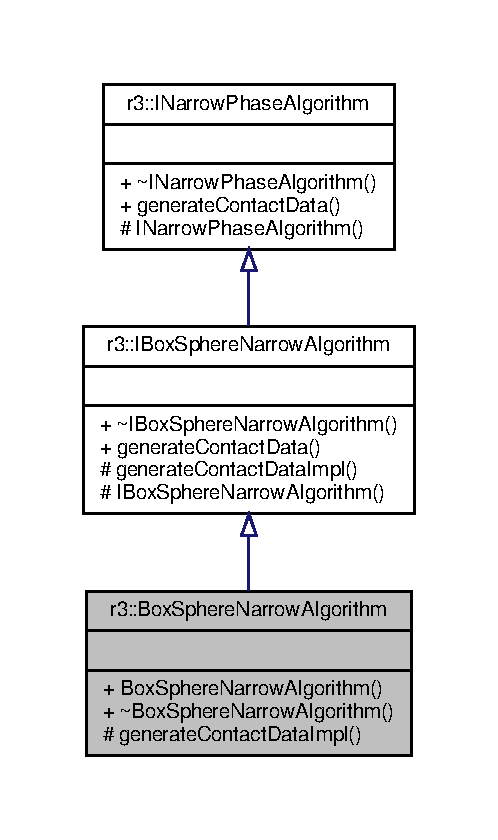
\includegraphics[width=239pt]{classr3_1_1_box_sphere_narrow_algorithm__inherit__graph}
\end{center}
\end{figure}


Collaboration diagram for r3\+:\+:Box\+Sphere\+Narrow\+Algorithm\+:\nopagebreak
\begin{figure}[H]
\begin{center}
\leavevmode
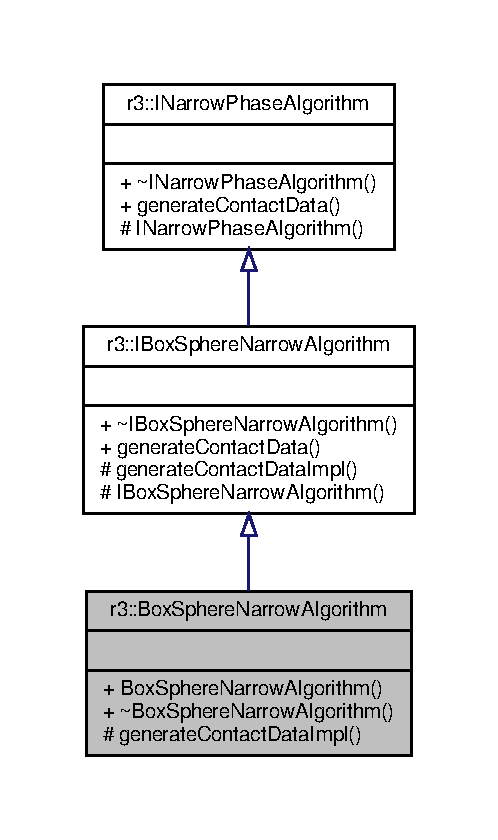
\includegraphics[width=239pt]{classr3_1_1_box_sphere_narrow_algorithm__coll__graph}
\end{center}
\end{figure}
\subsection*{Public Member Functions}
\begin{DoxyCompactItemize}
\item 
\mbox{\hyperlink{classr3_1_1_box_sphere_narrow_algorithm_a0184c33ce7da891240781ad7c78bd9a2}{Box\+Sphere\+Narrow\+Algorithm}} ()
\item 
\mbox{\hyperlink{classr3_1_1_box_sphere_narrow_algorithm_ab00e17b38da83e9a159aa7786a7a1f95}{$\sim$\+Box\+Sphere\+Narrow\+Algorithm}} ()
\end{DoxyCompactItemize}
\subsection*{Protected Member Functions}
\begin{DoxyCompactItemize}
\item 
bool \mbox{\hyperlink{classr3_1_1_box_sphere_narrow_algorithm_a2fc345fdec27e85f0e569afa0d500865}{generate\+Contact\+Data\+Impl}} (\mbox{\hyperlink{classr3_1_1_rigid_body}{Rigid\+Body}} $\ast$rb\+Box, \mbox{\hyperlink{classr3_1_1_collision_box}{Collision\+Box}} $\ast$box, \mbox{\hyperlink{classr3_1_1_rigid_body}{Rigid\+Body}} $\ast$rb\+Sphere, \mbox{\hyperlink{classr3_1_1_collision_sphere}{Collision\+Sphere}} $\ast$sphere, \mbox{\hyperlink{classr3_1_1_collision_data}{Collision\+Data}} \&collision\+Data) override
\end{DoxyCompactItemize}


\subsection{Detailed Description}
Default implementation for a box-\/sphere narrow algorithm. 

\subsection{Constructor \& Destructor Documentation}
\mbox{\Hypertarget{classr3_1_1_box_sphere_narrow_algorithm_a0184c33ce7da891240781ad7c78bd9a2}\label{classr3_1_1_box_sphere_narrow_algorithm_a0184c33ce7da891240781ad7c78bd9a2}} 
\index{r3\+::\+Box\+Sphere\+Narrow\+Algorithm@{r3\+::\+Box\+Sphere\+Narrow\+Algorithm}!Box\+Sphere\+Narrow\+Algorithm@{Box\+Sphere\+Narrow\+Algorithm}}
\index{Box\+Sphere\+Narrow\+Algorithm@{Box\+Sphere\+Narrow\+Algorithm}!r3\+::\+Box\+Sphere\+Narrow\+Algorithm@{r3\+::\+Box\+Sphere\+Narrow\+Algorithm}}
\subsubsection{\texorpdfstring{Box\+Sphere\+Narrow\+Algorithm()}{BoxSphereNarrowAlgorithm()}}
{\footnotesize\ttfamily r3\+::\+Box\+Sphere\+Narrow\+Algorithm\+::\+Box\+Sphere\+Narrow\+Algorithm (\begin{DoxyParamCaption}{ }\end{DoxyParamCaption})\hspace{0.3cm}{\ttfamily [explicit]}, {\ttfamily [default]}}

\mbox{\Hypertarget{classr3_1_1_box_sphere_narrow_algorithm_ab00e17b38da83e9a159aa7786a7a1f95}\label{classr3_1_1_box_sphere_narrow_algorithm_ab00e17b38da83e9a159aa7786a7a1f95}} 
\index{r3\+::\+Box\+Sphere\+Narrow\+Algorithm@{r3\+::\+Box\+Sphere\+Narrow\+Algorithm}!````~Box\+Sphere\+Narrow\+Algorithm@{$\sim$\+Box\+Sphere\+Narrow\+Algorithm}}
\index{````~Box\+Sphere\+Narrow\+Algorithm@{$\sim$\+Box\+Sphere\+Narrow\+Algorithm}!r3\+::\+Box\+Sphere\+Narrow\+Algorithm@{r3\+::\+Box\+Sphere\+Narrow\+Algorithm}}
\subsubsection{\texorpdfstring{$\sim$\+Box\+Sphere\+Narrow\+Algorithm()}{~BoxSphereNarrowAlgorithm()}}
{\footnotesize\ttfamily r3\+::\+Box\+Sphere\+Narrow\+Algorithm\+::$\sim$\+Box\+Sphere\+Narrow\+Algorithm (\begin{DoxyParamCaption}{ }\end{DoxyParamCaption})\hspace{0.3cm}{\ttfamily [default]}}



\subsection{Member Function Documentation}
\mbox{\Hypertarget{classr3_1_1_box_sphere_narrow_algorithm_a2fc345fdec27e85f0e569afa0d500865}\label{classr3_1_1_box_sphere_narrow_algorithm_a2fc345fdec27e85f0e569afa0d500865}} 
\index{r3\+::\+Box\+Sphere\+Narrow\+Algorithm@{r3\+::\+Box\+Sphere\+Narrow\+Algorithm}!generate\+Contact\+Data\+Impl@{generate\+Contact\+Data\+Impl}}
\index{generate\+Contact\+Data\+Impl@{generate\+Contact\+Data\+Impl}!r3\+::\+Box\+Sphere\+Narrow\+Algorithm@{r3\+::\+Box\+Sphere\+Narrow\+Algorithm}}
\subsubsection{\texorpdfstring{generate\+Contact\+Data\+Impl()}{generateContactDataImpl()}}
{\footnotesize\ttfamily bool r3\+::\+Box\+Sphere\+Narrow\+Algorithm\+::generate\+Contact\+Data\+Impl (\begin{DoxyParamCaption}\item[{\mbox{\hyperlink{classr3_1_1_rigid_body}{Rigid\+Body}} $\ast$}]{rb\+Box,  }\item[{\mbox{\hyperlink{classr3_1_1_collision_box}{Collision\+Box}} $\ast$}]{box,  }\item[{\mbox{\hyperlink{classr3_1_1_rigid_body}{Rigid\+Body}} $\ast$}]{rb\+Sphere,  }\item[{\mbox{\hyperlink{classr3_1_1_collision_sphere}{Collision\+Sphere}} $\ast$}]{sphere,  }\item[{\mbox{\hyperlink{classr3_1_1_collision_data}{Collision\+Data}} \&}]{collision\+Data }\end{DoxyParamCaption})\hspace{0.3cm}{\ttfamily [override]}, {\ttfamily [protected]}, {\ttfamily [virtual]}}



Implements \mbox{\hyperlink{classr3_1_1_i_box_sphere_narrow_algorithm_af28bcda3eb527a6ee48a3b624e5d47e0}{r3\+::\+I\+Box\+Sphere\+Narrow\+Algorithm}}.



The documentation for this class was generated from the following files\+:\begin{DoxyCompactItemize}
\item 
D\+:/\+Programming/\+Repositories/\+Game\+Physics/\+Simulation\+Visualization/\+Rumble3\+D/\+Rumble3\+D/include/\+R3\+D/\+Rigid\+Body\+Engine/\+Collision\+Detection/\+Algorithm/\mbox{\hyperlink{_box_sphere_narrow_algorithm_8h}{Box\+Sphere\+Narrow\+Algorithm.\+h}}\item 
D\+:/\+Programming/\+Repositories/\+Game\+Physics/\+Simulation\+Visualization/\+Rumble3\+D/\+Rumble3\+D/src/\+Rigid\+Body\+Engine/\+Collision\+Detection/\+Algorithm/\mbox{\hyperlink{_box_sphere_narrow_algorithm_8cpp}{Box\+Sphere\+Narrow\+Algorithm.\+cpp}}\end{DoxyCompactItemize}

\hypertarget{classr3_1_1_broad_phase_filter}{}\section{r3\+:\+:Broad\+Phase\+Filter Class Reference}
\label{classr3_1_1_broad_phase_filter}\index{r3\+::\+Broad\+Phase\+Filter@{r3\+::\+Broad\+Phase\+Filter}}


Default implementation of \mbox{\hyperlink{classr3_1_1_i_broad_phase_filter}{I\+Broad\+Phase\+Filter}}.  




{\ttfamily \#include $<$Broad\+Phase\+Filter.\+h$>$}



Inheritance diagram for r3\+:\+:Broad\+Phase\+Filter\+:\nopagebreak
\begin{figure}[H]
\begin{center}
\leavevmode
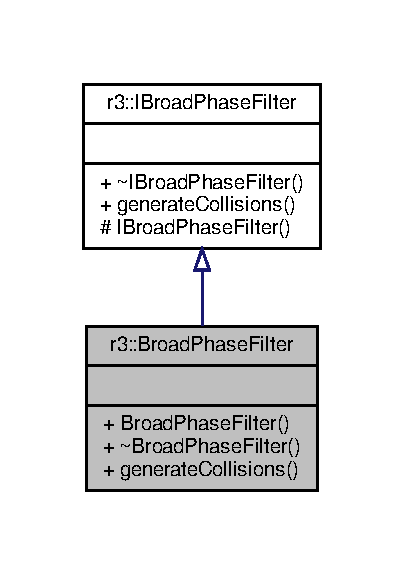
\includegraphics[width=195pt]{classr3_1_1_broad_phase_filter__inherit__graph}
\end{center}
\end{figure}


Collaboration diagram for r3\+:\+:Broad\+Phase\+Filter\+:\nopagebreak
\begin{figure}[H]
\begin{center}
\leavevmode
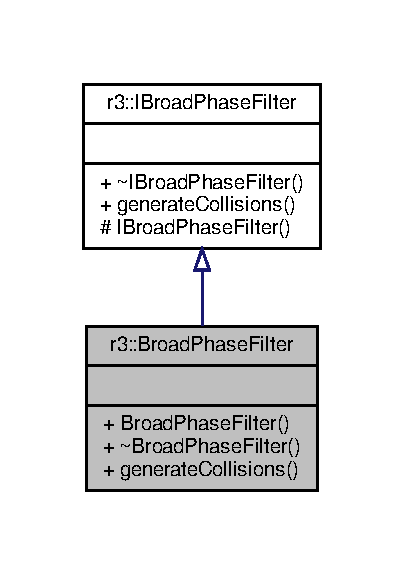
\includegraphics[width=195pt]{classr3_1_1_broad_phase_filter__coll__graph}
\end{center}
\end{figure}
\subsection*{Public Member Functions}
\begin{DoxyCompactItemize}
\item 
\mbox{\hyperlink{classr3_1_1_broad_phase_filter_afcdb0ed5acb941bf16e284cb0031fe2e}{Broad\+Phase\+Filter}} ()
\item 
\mbox{\hyperlink{classr3_1_1_broad_phase_filter_a3c28ac36ed06766b235efad77ff9fd5d}{$\sim$\+Broad\+Phase\+Filter}} ()
\item 
void \mbox{\hyperlink{classr3_1_1_broad_phase_filter_a0435dc6468401e32bf151f84f52e80f8}{generate\+Collisions}} (const std\+::vector$<$ \mbox{\hyperlink{classr3_1_1_rigid_body}{Rigid\+Body}} $\ast$$>$ \&rigid\+Bodies, \mbox{\hyperlink{classr3_1_1_fixed_size_container}{Fixed\+Size\+Container}}$<$ \mbox{\hyperlink{classr3_1_1_collision_pair}{Collision\+Pair}} $>$ \&data) override
\begin{DoxyCompactList}\small\item\em Conservatively check, which rigid body pairs might collide. These collisions can be false positives, but there should never be false negatives. \end{DoxyCompactList}\end{DoxyCompactItemize}
\subsection*{Additional Inherited Members}


\subsection{Detailed Description}
Default implementation of \mbox{\hyperlink{classr3_1_1_i_broad_phase_filter}{I\+Broad\+Phase\+Filter}}. 

\subsection{Constructor \& Destructor Documentation}
\mbox{\Hypertarget{classr3_1_1_broad_phase_filter_afcdb0ed5acb941bf16e284cb0031fe2e}\label{classr3_1_1_broad_phase_filter_afcdb0ed5acb941bf16e284cb0031fe2e}} 
\index{r3\+::\+Broad\+Phase\+Filter@{r3\+::\+Broad\+Phase\+Filter}!Broad\+Phase\+Filter@{Broad\+Phase\+Filter}}
\index{Broad\+Phase\+Filter@{Broad\+Phase\+Filter}!r3\+::\+Broad\+Phase\+Filter@{r3\+::\+Broad\+Phase\+Filter}}
\subsubsection{\texorpdfstring{Broad\+Phase\+Filter()}{BroadPhaseFilter()}}
{\footnotesize\ttfamily r3\+::\+Broad\+Phase\+Filter\+::\+Broad\+Phase\+Filter (\begin{DoxyParamCaption}{ }\end{DoxyParamCaption})\hspace{0.3cm}{\ttfamily [explicit]}, {\ttfamily [default]}}

\mbox{\Hypertarget{classr3_1_1_broad_phase_filter_a3c28ac36ed06766b235efad77ff9fd5d}\label{classr3_1_1_broad_phase_filter_a3c28ac36ed06766b235efad77ff9fd5d}} 
\index{r3\+::\+Broad\+Phase\+Filter@{r3\+::\+Broad\+Phase\+Filter}!````~Broad\+Phase\+Filter@{$\sim$\+Broad\+Phase\+Filter}}
\index{````~Broad\+Phase\+Filter@{$\sim$\+Broad\+Phase\+Filter}!r3\+::\+Broad\+Phase\+Filter@{r3\+::\+Broad\+Phase\+Filter}}
\subsubsection{\texorpdfstring{$\sim$\+Broad\+Phase\+Filter()}{~BroadPhaseFilter()}}
{\footnotesize\ttfamily r3\+::\+Broad\+Phase\+Filter\+::$\sim$\+Broad\+Phase\+Filter (\begin{DoxyParamCaption}{ }\end{DoxyParamCaption})\hspace{0.3cm}{\ttfamily [default]}}



\subsection{Member Function Documentation}
\mbox{\Hypertarget{classr3_1_1_broad_phase_filter_a0435dc6468401e32bf151f84f52e80f8}\label{classr3_1_1_broad_phase_filter_a0435dc6468401e32bf151f84f52e80f8}} 
\index{r3\+::\+Broad\+Phase\+Filter@{r3\+::\+Broad\+Phase\+Filter}!generate\+Collisions@{generate\+Collisions}}
\index{generate\+Collisions@{generate\+Collisions}!r3\+::\+Broad\+Phase\+Filter@{r3\+::\+Broad\+Phase\+Filter}}
\subsubsection{\texorpdfstring{generate\+Collisions()}{generateCollisions()}}
{\footnotesize\ttfamily void r3\+::\+Broad\+Phase\+Filter\+::generate\+Collisions (\begin{DoxyParamCaption}\item[{const std\+::vector$<$ \mbox{\hyperlink{classr3_1_1_rigid_body}{Rigid\+Body}} $\ast$$>$ \&}]{rigid\+Bodies,  }\item[{\mbox{\hyperlink{classr3_1_1_fixed_size_container}{Fixed\+Size\+Container}}$<$ \mbox{\hyperlink{classr3_1_1_collision_pair}{Collision\+Pair}} $>$ \&}]{data }\end{DoxyParamCaption})\hspace{0.3cm}{\ttfamily [override]}, {\ttfamily [virtual]}}



Conservatively check, which rigid body pairs might collide. These collisions can be false positives, but there should never be false negatives. 


\begin{DoxyParams}[1]{Parameters}
 & {\em rigid\+Bodies} & The rigid bodies to check against possible collisions. \\
\hline
\mbox{\tt out}  & {\em data} & A number of possible collisions. \\
\hline
\end{DoxyParams}
\begin{DoxyRefDesc}{Todo}
\item[\mbox{\hyperlink{todo__todo000013}{Todo}}]use rigid body mask and layout \end{DoxyRefDesc}


Implements \mbox{\hyperlink{classr3_1_1_i_broad_phase_filter_a5f437f6390a8f10bf96d72e35e3b4432}{r3\+::\+I\+Broad\+Phase\+Filter}}.



The documentation for this class was generated from the following files\+:\begin{DoxyCompactItemize}
\item 
D\+:/\+Library/\+Documents/\+Job/\+Forschungsmaster/\+Projekte/\+Simulation\+Visualization/\+Rumble3\+D/\+Rumble3\+D/include/\+R3\+D/\+Rigid\+Body\+Engine/\+Collision\+Detection/\mbox{\hyperlink{_broad_phase_filter_8h}{Broad\+Phase\+Filter.\+h}}\item 
D\+:/\+Library/\+Documents/\+Job/\+Forschungsmaster/\+Projekte/\+Simulation\+Visualization/\+Rumble3\+D/\+Rumble3\+D/src/\+Rigid\+Body\+Engine/\+Collision\+Detection/\mbox{\hyperlink{_broad_phase_filter_8cpp}{Broad\+Phase\+Filter.\+cpp}}\end{DoxyCompactItemize}

\hypertarget{classr3_1_1_b_v_h_node}{}\section{r3\+:\+:B\+V\+H\+Node$<$ Bounding\+Volume\+Class $>$ Class Template Reference}
\label{classr3_1_1_b_v_h_node}\index{r3\+::\+B\+V\+H\+Node$<$ Bounding\+Volume\+Class $>$@{r3\+::\+B\+V\+H\+Node$<$ Bounding\+Volume\+Class $>$}}


{\ttfamily \#include $<$B\+V\+H\+Node.\+h$>$}



Collaboration diagram for r3\+:\+:B\+V\+H\+Node$<$ Bounding\+Volume\+Class $>$\+:\nopagebreak
\begin{figure}[H]
\begin{center}
\leavevmode
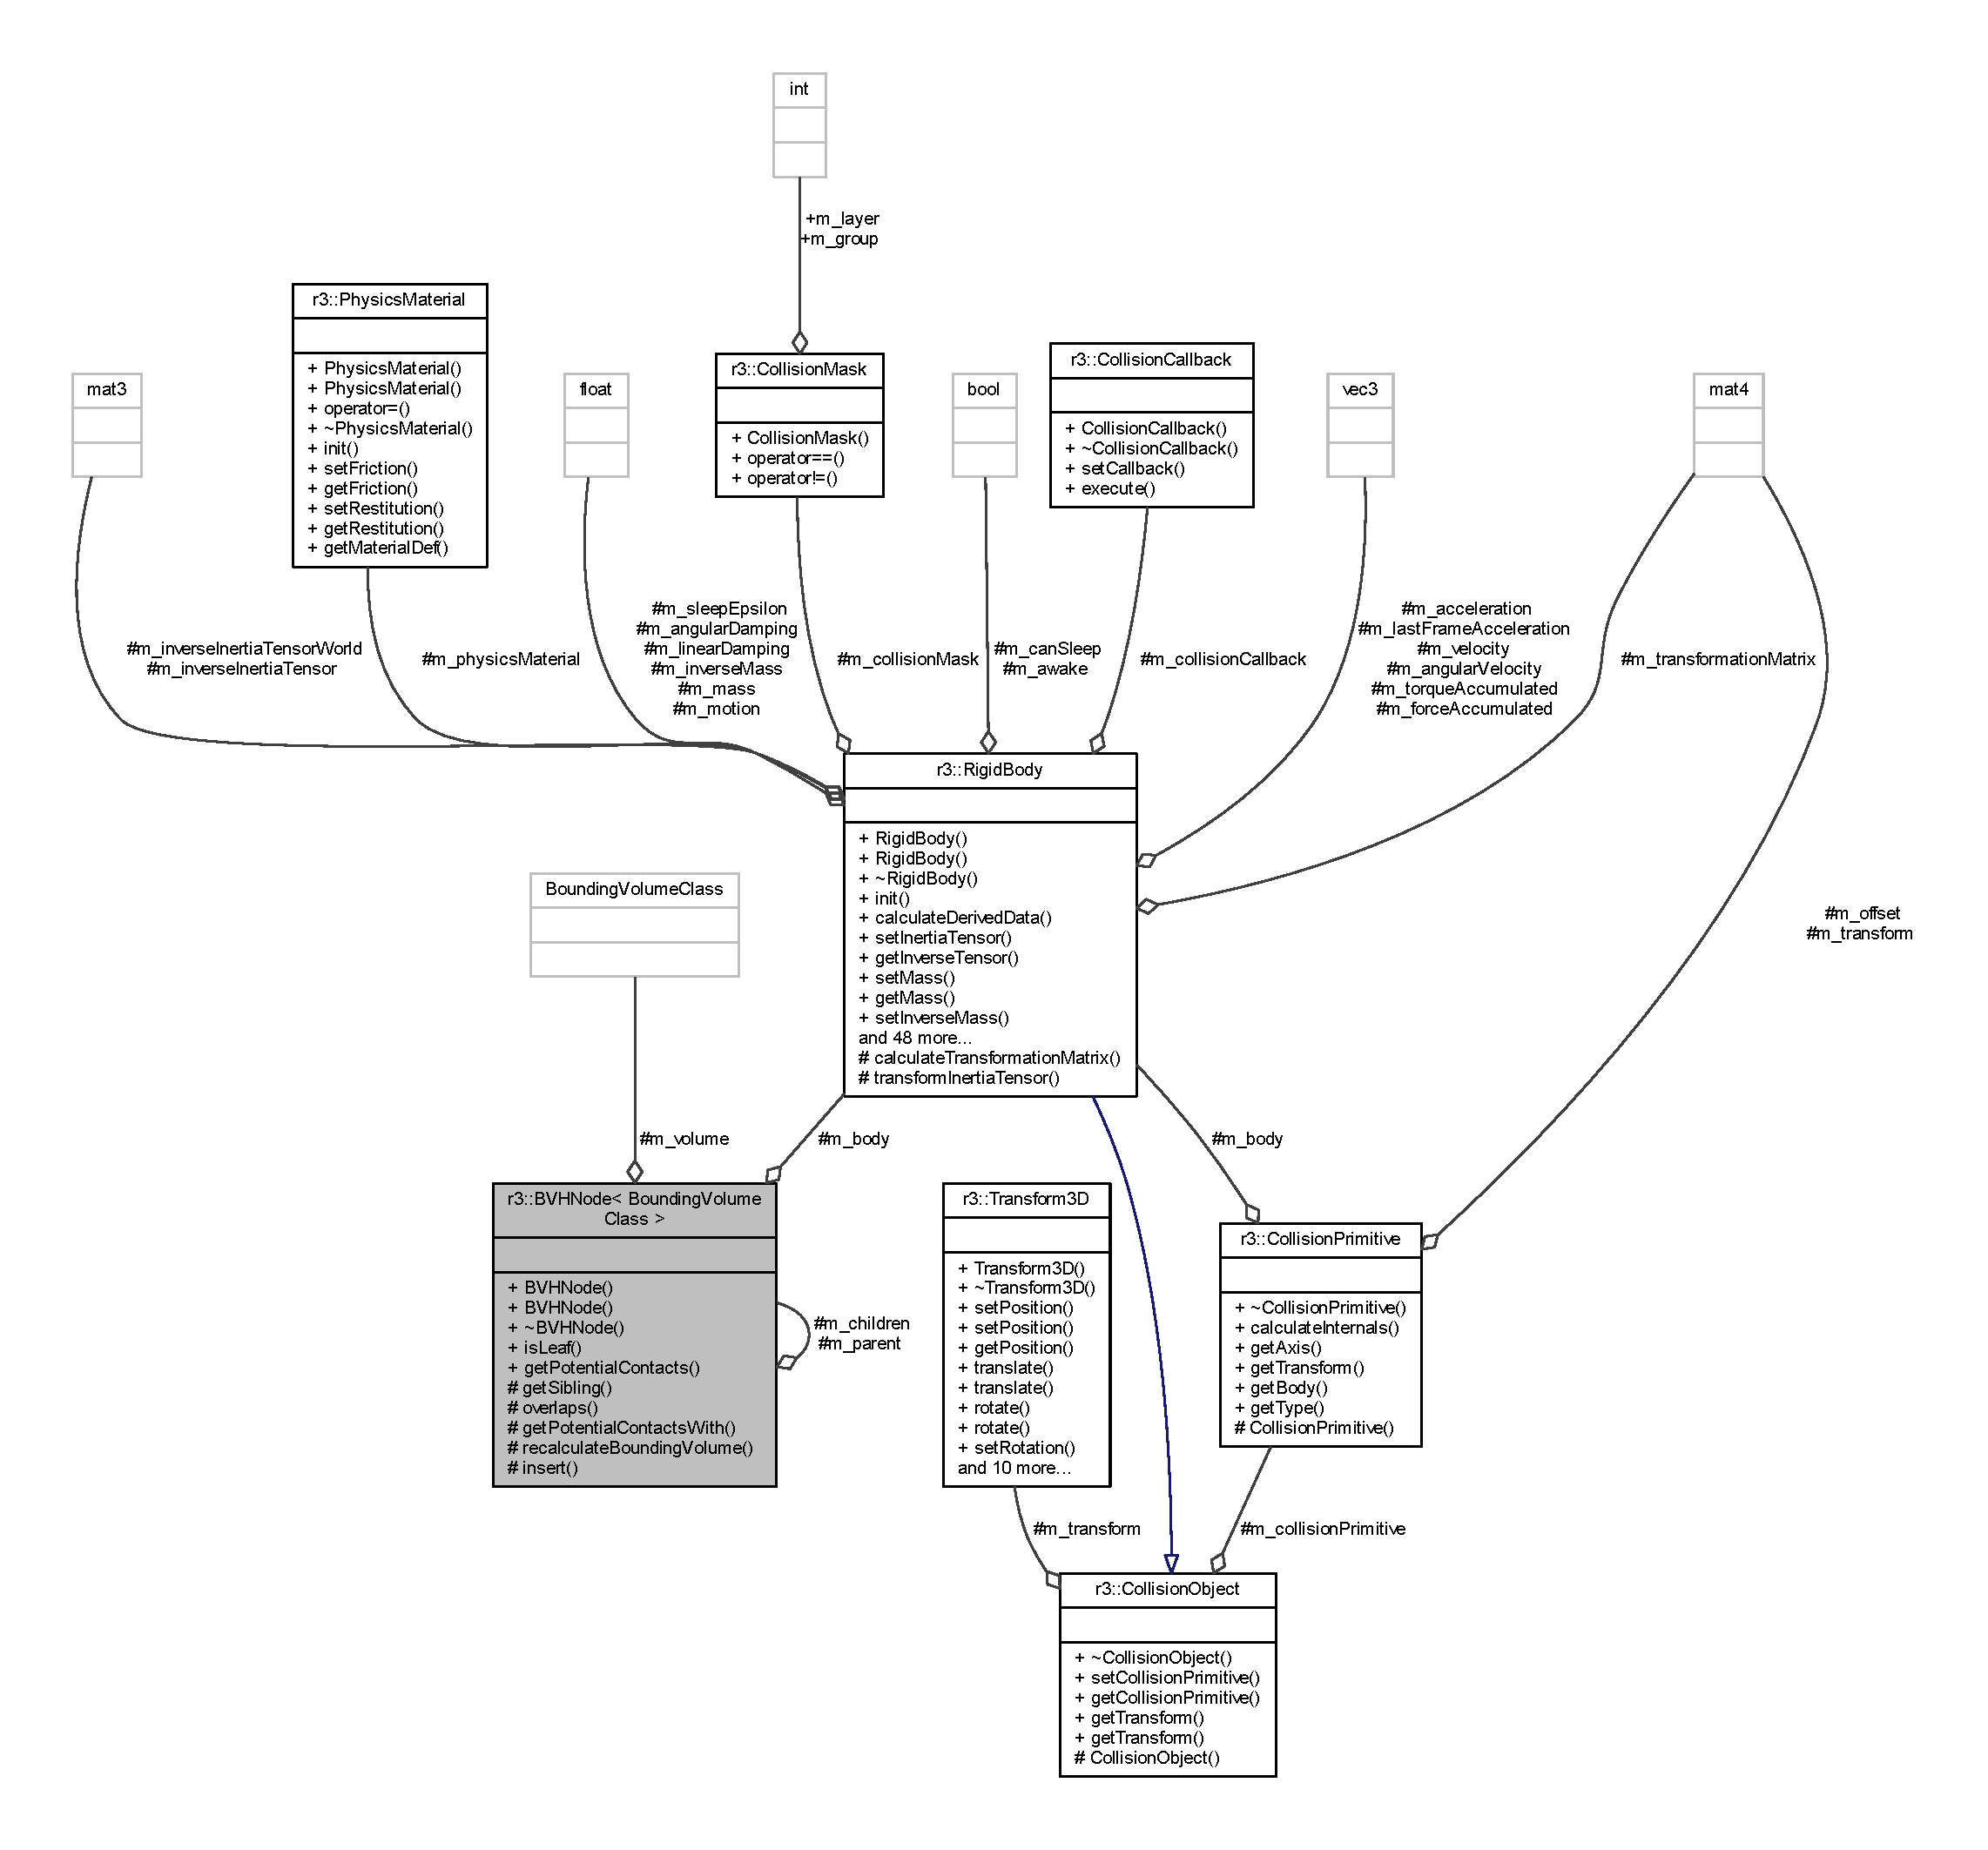
\includegraphics[width=350pt]{classr3_1_1_b_v_h_node__coll__graph}
\end{center}
\end{figure}
\subsection*{Public Member Functions}
\begin{DoxyCompactItemize}
\item 
\mbox{\hyperlink{classr3_1_1_b_v_h_node_a31b8beb2d10f5df915be92eab4bdd7f6}{B\+V\+H\+Node}} ()
\item 
\mbox{\hyperlink{classr3_1_1_b_v_h_node_a983ae7d4ab515427436692b8a846da6f}{B\+V\+H\+Node}} (\mbox{\hyperlink{classr3_1_1_b_v_h_node}{B\+V\+H\+Node}}$<$ Bounding\+Volume\+Class $>$ $\ast$parent, const Bounding\+Volume\+Class \&volume, \mbox{\hyperlink{classr3_1_1_rigid_body}{Rigid\+Body}} $\ast$body=nullptr)
\begin{DoxyCompactList}\small\item\em \mbox{\hyperlink{classr3_1_1_b_v_h_node}{B\+V\+H\+Node}} constructor. \end{DoxyCompactList}\item 
\mbox{\hyperlink{classr3_1_1_b_v_h_node_a72194bd522058bfd362b0ab77c0303af}{$\sim$\+B\+V\+H\+Node}} ()
\item 
bool \mbox{\hyperlink{classr3_1_1_b_v_h_node_a517b40f1a91cda371b3cb786f1c7e155}{is\+Leaf}} () const
\begin{DoxyCompactList}\small\item\em Check if this node is a leaf node (= has no child nodes). \end{DoxyCompactList}\item 
void \mbox{\hyperlink{classr3_1_1_b_v_h_node_a922773e61c14d365f2b9c9740d565783}{get\+Potential\+Contacts}} (\mbox{\hyperlink{classr3_1_1_fixed_size_container}{Fixed\+Size\+Container}}$<$ \mbox{\hyperlink{classr3_1_1_collision_pair}{Collision\+Pair}} $>$ \&contacts) const
\begin{DoxyCompactList}\small\item\em Find all potential contacts in this bounding volume hierarchy. \end{DoxyCompactList}\end{DoxyCompactItemize}
\subsection*{Protected Member Functions}
\begin{DoxyCompactItemize}
\item 
\mbox{\hyperlink{classr3_1_1_b_v_h_node}{B\+V\+H\+Node}}$<$ Bounding\+Volume\+Class $>$ $\ast$ \mbox{\hyperlink{classr3_1_1_b_v_h_node_ae2844615a68ba58f1379dd864f335633}{get\+Sibling}} () const
\begin{DoxyCompactList}\small\item\em Get the sibling node of a child node. \end{DoxyCompactList}\item 
bool \mbox{\hyperlink{classr3_1_1_b_v_h_node_a69ec6f958bbe07629cd979599532dfd8}{overlaps}} (\mbox{\hyperlink{classr3_1_1_b_v_h_node}{B\+V\+H\+Node}}$<$ Bounding\+Volume\+Class $>$ $\ast$other) const
\begin{DoxyCompactList}\small\item\em Check if there is a child node, that overlaps with the given node. \end{DoxyCompactList}\item 
void \mbox{\hyperlink{classr3_1_1_b_v_h_node_a00031bc5ca7a6971a396cad6ff3fe490}{get\+Potential\+Contacts\+With}} (\mbox{\hyperlink{classr3_1_1_b_v_h_node}{B\+V\+H\+Node}}$<$ Bounding\+Volume\+Class $>$ $\ast$other, \mbox{\hyperlink{classr3_1_1_fixed_size_container}{Fixed\+Size\+Container}}$<$ \mbox{\hyperlink{classr3_1_1_collision_pair}{Collision\+Pair}} $>$ \&contacts) const
\begin{DoxyCompactList}\small\item\em Get all potential contacts with the given bounding volume. \end{DoxyCompactList}\item 
void \mbox{\hyperlink{classr3_1_1_b_v_h_node_a52539a0d78d758021a2fe4bedd30e671}{recalculate\+Bounding\+Volume}} ()
\begin{DoxyCompactList}\small\item\em Recalculate all bounding volumes from this node all the way up to the root node. \end{DoxyCompactList}\item 
void \mbox{\hyperlink{classr3_1_1_b_v_h_node_ab6f91727e36689a7edc9f8c168ab904b}{insert}} (\mbox{\hyperlink{classr3_1_1_rigid_body}{Rigid\+Body}} $\ast$new\+Body, const Bounding\+Volume\+Class \&new\+Volume)
\begin{DoxyCompactList}\small\item\em Insert a new bounding volume into this B\+VH as a child node. \end{DoxyCompactList}\end{DoxyCompactItemize}
\subsection*{Protected Attributes}
\begin{DoxyCompactItemize}
\item 
\mbox{\hyperlink{classr3_1_1_b_v_h_node}{B\+V\+H\+Node}} $\ast$ \mbox{\hyperlink{classr3_1_1_b_v_h_node_a62424473dd79cf59262a6a53995b0e26}{m\+\_\+parent}}
\item 
\mbox{\hyperlink{classr3_1_1_b_v_h_node}{B\+V\+H\+Node}} $\ast$ \mbox{\hyperlink{classr3_1_1_b_v_h_node_ac3df92e9a175e4037a07801e1cca73db}{m\+\_\+children}} \mbox{[}2\mbox{]} \{\}
\item 
\mbox{\hyperlink{classr3_1_1_rigid_body}{Rigid\+Body}} $\ast$ \mbox{\hyperlink{classr3_1_1_b_v_h_node_a7f1a7f51f17ed00cc39298ff4d1f1d57}{m\+\_\+body}}
\begin{DoxyCompactList}\small\item\em Only set for leaf nodes. \end{DoxyCompactList}\item 
Bounding\+Volume\+Class \mbox{\hyperlink{classr3_1_1_b_v_h_node_a114366b1f5cbb56f6f650f9c794258a7}{m\+\_\+volume}}
\begin{DoxyCompactList}\small\item\em Bounding volume, which contains all child nodes. \end{DoxyCompactList}\end{DoxyCompactItemize}


\subsection{Detailed Description}
\subsubsection*{template$<$class Bounding\+Volume\+Class$>$\newline
class r3\+::\+B\+V\+H\+Node$<$ Bounding\+Volume\+Class $>$}

Hierarchy of bounding volumes. Only leaf nodes describe actually collidable bounding volumes. 

\subsection{Constructor \& Destructor Documentation}
\mbox{\Hypertarget{classr3_1_1_b_v_h_node_a31b8beb2d10f5df915be92eab4bdd7f6}\label{classr3_1_1_b_v_h_node_a31b8beb2d10f5df915be92eab4bdd7f6}} 
\index{r3\+::\+B\+V\+H\+Node@{r3\+::\+B\+V\+H\+Node}!B\+V\+H\+Node@{B\+V\+H\+Node}}
\index{B\+V\+H\+Node@{B\+V\+H\+Node}!r3\+::\+B\+V\+H\+Node@{r3\+::\+B\+V\+H\+Node}}
\subsubsection{\texorpdfstring{B\+V\+H\+Node()}{BVHNode()}\hspace{0.1cm}{\footnotesize\ttfamily [1/2]}}
{\footnotesize\ttfamily template$<$class Bounding\+Volume\+Class $>$ \\
\mbox{\hyperlink{classr3_1_1_b_v_h_node}{r3\+::\+B\+V\+H\+Node}}$<$ Bounding\+Volume\+Class $>$\+::\mbox{\hyperlink{classr3_1_1_b_v_h_node}{B\+V\+H\+Node}} (\begin{DoxyParamCaption}{ }\end{DoxyParamCaption})\hspace{0.3cm}{\ttfamily [default]}}

\mbox{\Hypertarget{classr3_1_1_b_v_h_node_a983ae7d4ab515427436692b8a846da6f}\label{classr3_1_1_b_v_h_node_a983ae7d4ab515427436692b8a846da6f}} 
\index{r3\+::\+B\+V\+H\+Node@{r3\+::\+B\+V\+H\+Node}!B\+V\+H\+Node@{B\+V\+H\+Node}}
\index{B\+V\+H\+Node@{B\+V\+H\+Node}!r3\+::\+B\+V\+H\+Node@{r3\+::\+B\+V\+H\+Node}}
\subsubsection{\texorpdfstring{B\+V\+H\+Node()}{BVHNode()}\hspace{0.1cm}{\footnotesize\ttfamily [2/2]}}
{\footnotesize\ttfamily template$<$class Bounding\+Volume\+Class $>$ \\
\mbox{\hyperlink{classr3_1_1_b_v_h_node}{r3\+::\+B\+V\+H\+Node}}$<$ Bounding\+Volume\+Class $>$\+::\mbox{\hyperlink{classr3_1_1_b_v_h_node}{B\+V\+H\+Node}} (\begin{DoxyParamCaption}\item[{\mbox{\hyperlink{classr3_1_1_b_v_h_node}{B\+V\+H\+Node}}$<$ Bounding\+Volume\+Class $>$ $\ast$}]{parent,  }\item[{const Bounding\+Volume\+Class \&}]{volume,  }\item[{\mbox{\hyperlink{classr3_1_1_rigid_body}{Rigid\+Body}} $\ast$}]{body = {\ttfamily nullptr} }\end{DoxyParamCaption})}



\mbox{\hyperlink{classr3_1_1_b_v_h_node}{B\+V\+H\+Node}} constructor. 


\begin{DoxyParams}{Parameters}
{\em parent} & The parent bounding volume. \\
\hline
{\em volume} & The bounding volume of this node which, contains all child bounding volumes. \\
\hline
{\em body} & The rigid body represented by this node. Should be nullptr for non-\/leaf nodes. \\
\hline
\end{DoxyParams}
\mbox{\Hypertarget{classr3_1_1_b_v_h_node_a72194bd522058bfd362b0ab77c0303af}\label{classr3_1_1_b_v_h_node_a72194bd522058bfd362b0ab77c0303af}} 
\index{r3\+::\+B\+V\+H\+Node@{r3\+::\+B\+V\+H\+Node}!````~B\+V\+H\+Node@{$\sim$\+B\+V\+H\+Node}}
\index{````~B\+V\+H\+Node@{$\sim$\+B\+V\+H\+Node}!r3\+::\+B\+V\+H\+Node@{r3\+::\+B\+V\+H\+Node}}
\subsubsection{\texorpdfstring{$\sim$\+B\+V\+H\+Node()}{~BVHNode()}}
{\footnotesize\ttfamily template$<$class Bounding\+Volume\+Class $>$ \\
\mbox{\hyperlink{classr3_1_1_b_v_h_node}{r3\+::\+B\+V\+H\+Node}}$<$ Bounding\+Volume\+Class $>$\+::$\sim$\mbox{\hyperlink{classr3_1_1_b_v_h_node}{B\+V\+H\+Node}} (\begin{DoxyParamCaption}{ }\end{DoxyParamCaption})}



\subsection{Member Function Documentation}
\mbox{\Hypertarget{classr3_1_1_b_v_h_node_a922773e61c14d365f2b9c9740d565783}\label{classr3_1_1_b_v_h_node_a922773e61c14d365f2b9c9740d565783}} 
\index{r3\+::\+B\+V\+H\+Node@{r3\+::\+B\+V\+H\+Node}!get\+Potential\+Contacts@{get\+Potential\+Contacts}}
\index{get\+Potential\+Contacts@{get\+Potential\+Contacts}!r3\+::\+B\+V\+H\+Node@{r3\+::\+B\+V\+H\+Node}}
\subsubsection{\texorpdfstring{get\+Potential\+Contacts()}{getPotentialContacts()}}
{\footnotesize\ttfamily template$<$class Bounding\+Volume\+Class $>$ \\
void \mbox{\hyperlink{classr3_1_1_b_v_h_node}{r3\+::\+B\+V\+H\+Node}}$<$ Bounding\+Volume\+Class $>$\+::get\+Potential\+Contacts (\begin{DoxyParamCaption}\item[{\mbox{\hyperlink{classr3_1_1_fixed_size_container}{Fixed\+Size\+Container}}$<$ \mbox{\hyperlink{classr3_1_1_collision_pair}{Collision\+Pair}} $>$ \&}]{contacts }\end{DoxyParamCaption}) const}



Find all potential contacts in this bounding volume hierarchy. 


\begin{DoxyParams}[1]{Parameters}
\mbox{\tt out}  & {\em contacts} & The resulting contacts. \\
\hline
\end{DoxyParams}
\mbox{\Hypertarget{classr3_1_1_b_v_h_node_a00031bc5ca7a6971a396cad6ff3fe490}\label{classr3_1_1_b_v_h_node_a00031bc5ca7a6971a396cad6ff3fe490}} 
\index{r3\+::\+B\+V\+H\+Node@{r3\+::\+B\+V\+H\+Node}!get\+Potential\+Contacts\+With@{get\+Potential\+Contacts\+With}}
\index{get\+Potential\+Contacts\+With@{get\+Potential\+Contacts\+With}!r3\+::\+B\+V\+H\+Node@{r3\+::\+B\+V\+H\+Node}}
\subsubsection{\texorpdfstring{get\+Potential\+Contacts\+With()}{getPotentialContactsWith()}}
{\footnotesize\ttfamily template$<$class Bounding\+Volume\+Class $>$ \\
void \mbox{\hyperlink{classr3_1_1_b_v_h_node}{r3\+::\+B\+V\+H\+Node}}$<$ Bounding\+Volume\+Class $>$\+::get\+Potential\+Contacts\+With (\begin{DoxyParamCaption}\item[{\mbox{\hyperlink{classr3_1_1_b_v_h_node}{B\+V\+H\+Node}}$<$ Bounding\+Volume\+Class $>$ $\ast$}]{other,  }\item[{\mbox{\hyperlink{classr3_1_1_fixed_size_container}{Fixed\+Size\+Container}}$<$ \mbox{\hyperlink{classr3_1_1_collision_pair}{Collision\+Pair}} $>$ \&}]{contacts }\end{DoxyParamCaption}) const\hspace{0.3cm}{\ttfamily [protected]}}



Get all potential contacts with the given bounding volume. 


\begin{DoxyParams}[1]{Parameters}
 & {\em other} & The bounding volume to check against. \\
\hline
\mbox{\tt out}  & {\em contacts} & The resulting contacts. \\
\hline
\end{DoxyParams}
Potential contact if both are leaf nodes. ~\newline
 Recursively get potential contacts with child nodes. \mbox{\Hypertarget{classr3_1_1_b_v_h_node_ae2844615a68ba58f1379dd864f335633}\label{classr3_1_1_b_v_h_node_ae2844615a68ba58f1379dd864f335633}} 
\index{r3\+::\+B\+V\+H\+Node@{r3\+::\+B\+V\+H\+Node}!get\+Sibling@{get\+Sibling}}
\index{get\+Sibling@{get\+Sibling}!r3\+::\+B\+V\+H\+Node@{r3\+::\+B\+V\+H\+Node}}
\subsubsection{\texorpdfstring{get\+Sibling()}{getSibling()}}
{\footnotesize\ttfamily template$<$class Bounding\+Volume\+Class $>$ \\
\mbox{\hyperlink{classr3_1_1_b_v_h_node}{B\+V\+H\+Node}}$<$ Bounding\+Volume\+Class $>$ $\ast$ \mbox{\hyperlink{classr3_1_1_b_v_h_node}{r3\+::\+B\+V\+H\+Node}}$<$ Bounding\+Volume\+Class $>$\+::get\+Sibling (\begin{DoxyParamCaption}{ }\end{DoxyParamCaption}) const\hspace{0.3cm}{\ttfamily [protected]}}



Get the sibling node of a child node. 

\begin{DoxyReturn}{Returns}
The sibling node or nullptr if this node has no parent. 
\end{DoxyReturn}
\mbox{\Hypertarget{classr3_1_1_b_v_h_node_ab6f91727e36689a7edc9f8c168ab904b}\label{classr3_1_1_b_v_h_node_ab6f91727e36689a7edc9f8c168ab904b}} 
\index{r3\+::\+B\+V\+H\+Node@{r3\+::\+B\+V\+H\+Node}!insert@{insert}}
\index{insert@{insert}!r3\+::\+B\+V\+H\+Node@{r3\+::\+B\+V\+H\+Node}}
\subsubsection{\texorpdfstring{insert()}{insert()}}
{\footnotesize\ttfamily template$<$class Bounding\+Volume\+Class $>$ \\
void \mbox{\hyperlink{classr3_1_1_b_v_h_node}{r3\+::\+B\+V\+H\+Node}}$<$ Bounding\+Volume\+Class $>$\+::insert (\begin{DoxyParamCaption}\item[{\mbox{\hyperlink{classr3_1_1_rigid_body}{Rigid\+Body}} $\ast$}]{new\+Body,  }\item[{const Bounding\+Volume\+Class \&}]{new\+Volume }\end{DoxyParamCaption})\hspace{0.3cm}{\ttfamily [protected]}}



Insert a new bounding volume into this B\+VH as a child node. 


\begin{DoxyParams}{Parameters}
{\em new\+Body} & The rigid body to insert. \\
\hline
{\em new\+Volume} & The new volume to insert. \\
\hline
\end{DoxyParams}
\mbox{\Hypertarget{classr3_1_1_b_v_h_node_a517b40f1a91cda371b3cb786f1c7e155}\label{classr3_1_1_b_v_h_node_a517b40f1a91cda371b3cb786f1c7e155}} 
\index{r3\+::\+B\+V\+H\+Node@{r3\+::\+B\+V\+H\+Node}!is\+Leaf@{is\+Leaf}}
\index{is\+Leaf@{is\+Leaf}!r3\+::\+B\+V\+H\+Node@{r3\+::\+B\+V\+H\+Node}}
\subsubsection{\texorpdfstring{is\+Leaf()}{isLeaf()}}
{\footnotesize\ttfamily template$<$class Bounding\+Volume\+Class $>$ \\
bool \mbox{\hyperlink{classr3_1_1_b_v_h_node}{r3\+::\+B\+V\+H\+Node}}$<$ Bounding\+Volume\+Class $>$\+::is\+Leaf (\begin{DoxyParamCaption}{ }\end{DoxyParamCaption}) const}



Check if this node is a leaf node (= has no child nodes). 

\begin{DoxyReturn}{Returns}
True if it is a leaf node, false otherwise. 
\end{DoxyReturn}
\mbox{\Hypertarget{classr3_1_1_b_v_h_node_a69ec6f958bbe07629cd979599532dfd8}\label{classr3_1_1_b_v_h_node_a69ec6f958bbe07629cd979599532dfd8}} 
\index{r3\+::\+B\+V\+H\+Node@{r3\+::\+B\+V\+H\+Node}!overlaps@{overlaps}}
\index{overlaps@{overlaps}!r3\+::\+B\+V\+H\+Node@{r3\+::\+B\+V\+H\+Node}}
\subsubsection{\texorpdfstring{overlaps()}{overlaps()}}
{\footnotesize\ttfamily template$<$class Bounding\+Volume\+Class $>$ \\
bool \mbox{\hyperlink{classr3_1_1_b_v_h_node}{r3\+::\+B\+V\+H\+Node}}$<$ Bounding\+Volume\+Class $>$\+::overlaps (\begin{DoxyParamCaption}\item[{\mbox{\hyperlink{classr3_1_1_b_v_h_node}{B\+V\+H\+Node}}$<$ Bounding\+Volume\+Class $>$ $\ast$}]{other }\end{DoxyParamCaption}) const\hspace{0.3cm}{\ttfamily [protected]}}



Check if there is a child node, that overlaps with the given node. 


\begin{DoxyParams}{Parameters}
{\em other} & The other node to check against. \\
\hline
\end{DoxyParams}
\begin{DoxyReturn}{Returns}
True if there is a collision, false otherwise. 
\end{DoxyReturn}
\mbox{\Hypertarget{classr3_1_1_b_v_h_node_a52539a0d78d758021a2fe4bedd30e671}\label{classr3_1_1_b_v_h_node_a52539a0d78d758021a2fe4bedd30e671}} 
\index{r3\+::\+B\+V\+H\+Node@{r3\+::\+B\+V\+H\+Node}!recalculate\+Bounding\+Volume@{recalculate\+Bounding\+Volume}}
\index{recalculate\+Bounding\+Volume@{recalculate\+Bounding\+Volume}!r3\+::\+B\+V\+H\+Node@{r3\+::\+B\+V\+H\+Node}}
\subsubsection{\texorpdfstring{recalculate\+Bounding\+Volume()}{recalculateBoundingVolume()}}
{\footnotesize\ttfamily template$<$class Bounding\+Volume\+Class $>$ \\
void \mbox{\hyperlink{classr3_1_1_b_v_h_node}{r3\+::\+B\+V\+H\+Node}}$<$ Bounding\+Volume\+Class $>$\+::recalculate\+Bounding\+Volume (\begin{DoxyParamCaption}{ }\end{DoxyParamCaption})\hspace{0.3cm}{\ttfamily [protected]}}



Recalculate all bounding volumes from this node all the way up to the root node. 



\subsection{Member Data Documentation}
\mbox{\Hypertarget{classr3_1_1_b_v_h_node_a7f1a7f51f17ed00cc39298ff4d1f1d57}\label{classr3_1_1_b_v_h_node_a7f1a7f51f17ed00cc39298ff4d1f1d57}} 
\index{r3\+::\+B\+V\+H\+Node@{r3\+::\+B\+V\+H\+Node}!m\+\_\+body@{m\+\_\+body}}
\index{m\+\_\+body@{m\+\_\+body}!r3\+::\+B\+V\+H\+Node@{r3\+::\+B\+V\+H\+Node}}
\subsubsection{\texorpdfstring{m\+\_\+body}{m\_body}}
{\footnotesize\ttfamily template$<$class Bounding\+Volume\+Class$>$ \\
\mbox{\hyperlink{classr3_1_1_rigid_body}{Rigid\+Body}}$\ast$ \mbox{\hyperlink{classr3_1_1_b_v_h_node}{r3\+::\+B\+V\+H\+Node}}$<$ Bounding\+Volume\+Class $>$\+::m\+\_\+body\hspace{0.3cm}{\ttfamily [protected]}}



Only set for leaf nodes. 

\mbox{\Hypertarget{classr3_1_1_b_v_h_node_ac3df92e9a175e4037a07801e1cca73db}\label{classr3_1_1_b_v_h_node_ac3df92e9a175e4037a07801e1cca73db}} 
\index{r3\+::\+B\+V\+H\+Node@{r3\+::\+B\+V\+H\+Node}!m\+\_\+children@{m\+\_\+children}}
\index{m\+\_\+children@{m\+\_\+children}!r3\+::\+B\+V\+H\+Node@{r3\+::\+B\+V\+H\+Node}}
\subsubsection{\texorpdfstring{m\+\_\+children}{m\_children}}
{\footnotesize\ttfamily template$<$class Bounding\+Volume\+Class$>$ \\
\mbox{\hyperlink{classr3_1_1_b_v_h_node}{B\+V\+H\+Node}}$\ast$ \mbox{\hyperlink{classr3_1_1_b_v_h_node}{r3\+::\+B\+V\+H\+Node}}$<$ Bounding\+Volume\+Class $>$\+::m\+\_\+children\mbox{[}2\mbox{]} \{\}\hspace{0.3cm}{\ttfamily [protected]}}

\mbox{\Hypertarget{classr3_1_1_b_v_h_node_a62424473dd79cf59262a6a53995b0e26}\label{classr3_1_1_b_v_h_node_a62424473dd79cf59262a6a53995b0e26}} 
\index{r3\+::\+B\+V\+H\+Node@{r3\+::\+B\+V\+H\+Node}!m\+\_\+parent@{m\+\_\+parent}}
\index{m\+\_\+parent@{m\+\_\+parent}!r3\+::\+B\+V\+H\+Node@{r3\+::\+B\+V\+H\+Node}}
\subsubsection{\texorpdfstring{m\+\_\+parent}{m\_parent}}
{\footnotesize\ttfamily template$<$class Bounding\+Volume\+Class$>$ \\
\mbox{\hyperlink{classr3_1_1_b_v_h_node}{B\+V\+H\+Node}}$\ast$ \mbox{\hyperlink{classr3_1_1_b_v_h_node}{r3\+::\+B\+V\+H\+Node}}$<$ Bounding\+Volume\+Class $>$\+::m\+\_\+parent\hspace{0.3cm}{\ttfamily [protected]}}

\mbox{\Hypertarget{classr3_1_1_b_v_h_node_a114366b1f5cbb56f6f650f9c794258a7}\label{classr3_1_1_b_v_h_node_a114366b1f5cbb56f6f650f9c794258a7}} 
\index{r3\+::\+B\+V\+H\+Node@{r3\+::\+B\+V\+H\+Node}!m\+\_\+volume@{m\+\_\+volume}}
\index{m\+\_\+volume@{m\+\_\+volume}!r3\+::\+B\+V\+H\+Node@{r3\+::\+B\+V\+H\+Node}}
\subsubsection{\texorpdfstring{m\+\_\+volume}{m\_volume}}
{\footnotesize\ttfamily template$<$class Bounding\+Volume\+Class$>$ \\
Bounding\+Volume\+Class \mbox{\hyperlink{classr3_1_1_b_v_h_node}{r3\+::\+B\+V\+H\+Node}}$<$ Bounding\+Volume\+Class $>$\+::m\+\_\+volume\hspace{0.3cm}{\ttfamily [protected]}}



Bounding volume, which contains all child nodes. 



The documentation for this class was generated from the following files\+:\begin{DoxyCompactItemize}
\item 
D\+:/\+Library/\+Documents/\+Job/\+Forschungsmaster/\+Projekte/\+Simulation\+Visualization/\+Rumble3\+D/\+Rumble3\+D/include/\+R3\+D/\+Rigid\+Body\+Engine/\mbox{\hyperlink{_b_v_h_node_8h}{B\+V\+H\+Node.\+h}}\item 
D\+:/\+Library/\+Documents/\+Job/\+Forschungsmaster/\+Projekte/\+Simulation\+Visualization/\+Rumble3\+D/\+Rumble3\+D/src/\+Rigid\+Body\+Engine/\mbox{\hyperlink{_b_v_h_node_8cpp}{B\+V\+H\+Node.\+cpp}}\end{DoxyCompactItemize}

\hypertarget{classr3_1_1_collision_algorithm_matrix}{}\section{r3\+:\+:Collision\+Algorithm\+Matrix Class Reference}
\label{classr3_1_1_collision_algorithm_matrix}\index{r3\+::\+Collision\+Algorithm\+Matrix@{r3\+::\+Collision\+Algorithm\+Matrix}}


Describes a collision algorithm for every collision primitive type combination.  




{\ttfamily \#include $<$Collision\+Algorithm\+Matrix.\+h$>$}



Collaboration diagram for r3\+:\+:Collision\+Algorithm\+Matrix\+:\nopagebreak
\begin{figure}[H]
\begin{center}
\leavevmode
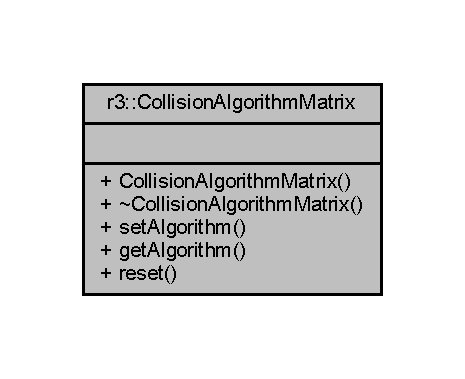
\includegraphics[width=223pt]{classr3_1_1_collision_algorithm_matrix__coll__graph}
\end{center}
\end{figure}
\subsection*{Public Types}
\begin{DoxyCompactItemize}
\item 
using \mbox{\hyperlink{classr3_1_1_collision_algorithm_matrix_ae68e99a7d5f10618fa4b82ee254052b9}{Algorithm\+\_\+\+Ptr}} = std\+::shared\+\_\+ptr$<$ \mbox{\hyperlink{classr3_1_1_i_narrow_phase_algorithm}{I\+Narrow\+Phase\+Algorithm}} $>$
\end{DoxyCompactItemize}
\subsection*{Public Member Functions}
\begin{DoxyCompactItemize}
\item 
\mbox{\hyperlink{classr3_1_1_collision_algorithm_matrix_a97bdad626057f600ae5ffca63eb174b8}{Collision\+Algorithm\+Matrix}} ()
\item 
\mbox{\hyperlink{classr3_1_1_collision_algorithm_matrix_adea2db794d9606ecf24745ad6ac912d8}{$\sim$\+Collision\+Algorithm\+Matrix}} ()
\item 
void \mbox{\hyperlink{classr3_1_1_collision_algorithm_matrix_a05aae40f6aba106fa9e62b45fd434bad}{set\+Algorithm}} (const \mbox{\hyperlink{classr3_1_1_collision_algorithm_matrix_ae68e99a7d5f10618fa4b82ee254052b9}{Algorithm\+\_\+\+Ptr}} \&algorithm, Collision\+Primitive\+Type first\+Shape, Collision\+Primitive\+Type second\+Shape)
\begin{DoxyCompactList}\small\item\em Set the collision algorithm for a specific collision primitive combination. \end{DoxyCompactList}\item 
\mbox{\hyperlink{classr3_1_1_i_narrow_phase_algorithm}{I\+Narrow\+Phase\+Algorithm}} $\ast$ \mbox{\hyperlink{classr3_1_1_collision_algorithm_matrix_ad40e0f125b95d6bcdb2e8a27c1397e68}{get\+Algorithm}} (Collision\+Primitive\+Type first\+Shape, Collision\+Primitive\+Type second\+Shape)
\begin{DoxyCompactList}\small\item\em Get the collision algorithm currently used for a specific collision primitive combination. \end{DoxyCompactList}\item 
void \mbox{\hyperlink{classr3_1_1_collision_algorithm_matrix_af2f1a16b0e3bbede20dc8559820525cb}{reset}} ()
\begin{DoxyCompactList}\small\item\em Replace all algorithms with a null algorithm. \end{DoxyCompactList}\end{DoxyCompactItemize}


\subsection{Detailed Description}
Describes a collision algorithm for every collision primitive type combination. 

\subsection{Member Typedef Documentation}
\mbox{\Hypertarget{classr3_1_1_collision_algorithm_matrix_ae68e99a7d5f10618fa4b82ee254052b9}\label{classr3_1_1_collision_algorithm_matrix_ae68e99a7d5f10618fa4b82ee254052b9}} 
\index{r3\+::\+Collision\+Algorithm\+Matrix@{r3\+::\+Collision\+Algorithm\+Matrix}!Algorithm\+\_\+\+Ptr@{Algorithm\+\_\+\+Ptr}}
\index{Algorithm\+\_\+\+Ptr@{Algorithm\+\_\+\+Ptr}!r3\+::\+Collision\+Algorithm\+Matrix@{r3\+::\+Collision\+Algorithm\+Matrix}}
\subsubsection{\texorpdfstring{Algorithm\+\_\+\+Ptr}{Algorithm\_Ptr}}
{\footnotesize\ttfamily using \mbox{\hyperlink{classr3_1_1_collision_algorithm_matrix_ae68e99a7d5f10618fa4b82ee254052b9}{r3\+::\+Collision\+Algorithm\+Matrix\+::\+Algorithm\+\_\+\+Ptr}} =  std\+::shared\+\_\+ptr$<$\mbox{\hyperlink{classr3_1_1_i_narrow_phase_algorithm}{I\+Narrow\+Phase\+Algorithm}}$>$}



\subsection{Constructor \& Destructor Documentation}
\mbox{\Hypertarget{classr3_1_1_collision_algorithm_matrix_a97bdad626057f600ae5ffca63eb174b8}\label{classr3_1_1_collision_algorithm_matrix_a97bdad626057f600ae5ffca63eb174b8}} 
\index{r3\+::\+Collision\+Algorithm\+Matrix@{r3\+::\+Collision\+Algorithm\+Matrix}!Collision\+Algorithm\+Matrix@{Collision\+Algorithm\+Matrix}}
\index{Collision\+Algorithm\+Matrix@{Collision\+Algorithm\+Matrix}!r3\+::\+Collision\+Algorithm\+Matrix@{r3\+::\+Collision\+Algorithm\+Matrix}}
\subsubsection{\texorpdfstring{Collision\+Algorithm\+Matrix()}{CollisionAlgorithmMatrix()}}
{\footnotesize\ttfamily r3\+::\+Collision\+Algorithm\+Matrix\+::\+Collision\+Algorithm\+Matrix (\begin{DoxyParamCaption}{ }\end{DoxyParamCaption})\hspace{0.3cm}{\ttfamily [explicit]}}

\mbox{\Hypertarget{classr3_1_1_collision_algorithm_matrix_adea2db794d9606ecf24745ad6ac912d8}\label{classr3_1_1_collision_algorithm_matrix_adea2db794d9606ecf24745ad6ac912d8}} 
\index{r3\+::\+Collision\+Algorithm\+Matrix@{r3\+::\+Collision\+Algorithm\+Matrix}!````~Collision\+Algorithm\+Matrix@{$\sim$\+Collision\+Algorithm\+Matrix}}
\index{````~Collision\+Algorithm\+Matrix@{$\sim$\+Collision\+Algorithm\+Matrix}!r3\+::\+Collision\+Algorithm\+Matrix@{r3\+::\+Collision\+Algorithm\+Matrix}}
\subsubsection{\texorpdfstring{$\sim$\+Collision\+Algorithm\+Matrix()}{~CollisionAlgorithmMatrix()}}
{\footnotesize\ttfamily r3\+::\+Collision\+Algorithm\+Matrix\+::$\sim$\+Collision\+Algorithm\+Matrix (\begin{DoxyParamCaption}{ }\end{DoxyParamCaption})\hspace{0.3cm}{\ttfamily [default]}}



\subsection{Member Function Documentation}
\mbox{\Hypertarget{classr3_1_1_collision_algorithm_matrix_ad40e0f125b95d6bcdb2e8a27c1397e68}\label{classr3_1_1_collision_algorithm_matrix_ad40e0f125b95d6bcdb2e8a27c1397e68}} 
\index{r3\+::\+Collision\+Algorithm\+Matrix@{r3\+::\+Collision\+Algorithm\+Matrix}!get\+Algorithm@{get\+Algorithm}}
\index{get\+Algorithm@{get\+Algorithm}!r3\+::\+Collision\+Algorithm\+Matrix@{r3\+::\+Collision\+Algorithm\+Matrix}}
\subsubsection{\texorpdfstring{get\+Algorithm()}{getAlgorithm()}}
{\footnotesize\ttfamily \mbox{\hyperlink{classr3_1_1_i_narrow_phase_algorithm}{I\+Narrow\+Phase\+Algorithm}} $\ast$ r3\+::\+Collision\+Algorithm\+Matrix\+::get\+Algorithm (\begin{DoxyParamCaption}\item[{Collision\+Primitive\+Type}]{first\+Shape,  }\item[{Collision\+Primitive\+Type}]{second\+Shape }\end{DoxyParamCaption})}



Get the collision algorithm currently used for a specific collision primitive combination. 


\begin{DoxyParams}{Parameters}
{\em first\+Shape} & The type of the first primitive shape. \\
\hline
{\em second\+Shape} & The type of the second primitive shape. \\
\hline
\end{DoxyParams}
\begin{DoxyReturn}{Returns}
The collision algorithm if existent, a null object otherwise. 
\end{DoxyReturn}
\mbox{\Hypertarget{classr3_1_1_collision_algorithm_matrix_af2f1a16b0e3bbede20dc8559820525cb}\label{classr3_1_1_collision_algorithm_matrix_af2f1a16b0e3bbede20dc8559820525cb}} 
\index{r3\+::\+Collision\+Algorithm\+Matrix@{r3\+::\+Collision\+Algorithm\+Matrix}!reset@{reset}}
\index{reset@{reset}!r3\+::\+Collision\+Algorithm\+Matrix@{r3\+::\+Collision\+Algorithm\+Matrix}}
\subsubsection{\texorpdfstring{reset()}{reset()}}
{\footnotesize\ttfamily void r3\+::\+Collision\+Algorithm\+Matrix\+::reset (\begin{DoxyParamCaption}{ }\end{DoxyParamCaption})}



Replace all algorithms with a null algorithm. 

\mbox{\Hypertarget{classr3_1_1_collision_algorithm_matrix_a05aae40f6aba106fa9e62b45fd434bad}\label{classr3_1_1_collision_algorithm_matrix_a05aae40f6aba106fa9e62b45fd434bad}} 
\index{r3\+::\+Collision\+Algorithm\+Matrix@{r3\+::\+Collision\+Algorithm\+Matrix}!set\+Algorithm@{set\+Algorithm}}
\index{set\+Algorithm@{set\+Algorithm}!r3\+::\+Collision\+Algorithm\+Matrix@{r3\+::\+Collision\+Algorithm\+Matrix}}
\subsubsection{\texorpdfstring{set\+Algorithm()}{setAlgorithm()}}
{\footnotesize\ttfamily void r3\+::\+Collision\+Algorithm\+Matrix\+::set\+Algorithm (\begin{DoxyParamCaption}\item[{const \mbox{\hyperlink{classr3_1_1_collision_algorithm_matrix_ae68e99a7d5f10618fa4b82ee254052b9}{Algorithm\+\_\+\+Ptr}} \&}]{algorithm,  }\item[{Collision\+Primitive\+Type}]{first\+Shape,  }\item[{Collision\+Primitive\+Type}]{second\+Shape }\end{DoxyParamCaption})}



Set the collision algorithm for a specific collision primitive combination. 


\begin{DoxyParams}{Parameters}
{\em algorithm} & The algorithm to use for the specified combination. \\
\hline
{\em first\+Shape} & The type of the first primitive shape. \\
\hline
{\em second\+Shape} & The type of the second shape. \\
\hline
\end{DoxyParams}


The documentation for this class was generated from the following files\+:\begin{DoxyCompactItemize}
\item 
D\+:/\+Programming/\+Repositories/\+Game\+Physics/\+Simulation\+Visualization/\+Rumble3\+D/\+Rumble3\+D/include/\+R3\+D/\+Rigid\+Body\+Engine/\+Collision\+Detection/\mbox{\hyperlink{_collision_algorithm_matrix_8h}{Collision\+Algorithm\+Matrix.\+h}}\item 
D\+:/\+Programming/\+Repositories/\+Game\+Physics/\+Simulation\+Visualization/\+Rumble3\+D/\+Rumble3\+D/src/\+Rigid\+Body\+Engine/\+Collision\+Detection/\mbox{\hyperlink{_collision_algorithm_matrix_8cpp}{Collision\+Algorithm\+Matrix.\+cpp}}\end{DoxyCompactItemize}

\hypertarget{classr3_1_1_collision_box}{}\section{r3\+:\+:Collision\+Box Class Reference}
\label{classr3_1_1_collision_box}\index{r3\+::\+Collision\+Box@{r3\+::\+Collision\+Box}}


\mbox{\hyperlink{classr3_1_1_collision_primitive}{Collision\+Primitive}} that represents a box.  




{\ttfamily \#include $<$Collision\+Box.\+h$>$}



Inheritance diagram for r3\+:\+:Collision\+Box\+:\nopagebreak
\begin{figure}[H]
\begin{center}
\leavevmode
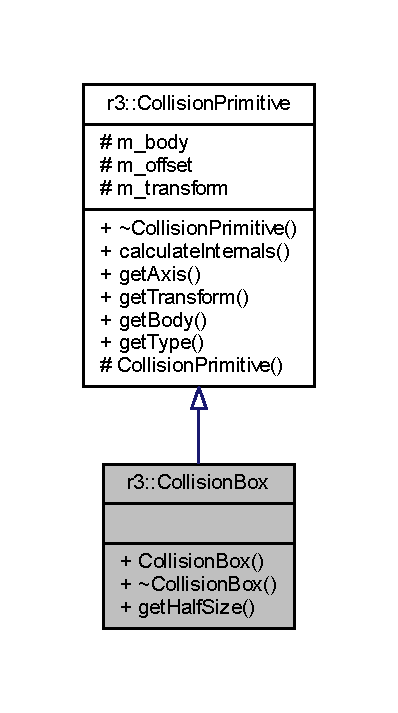
\includegraphics[width=191pt]{classr3_1_1_collision_box__inherit__graph}
\end{center}
\end{figure}


Collaboration diagram for r3\+:\+:Collision\+Box\+:\nopagebreak
\begin{figure}[H]
\begin{center}
\leavevmode
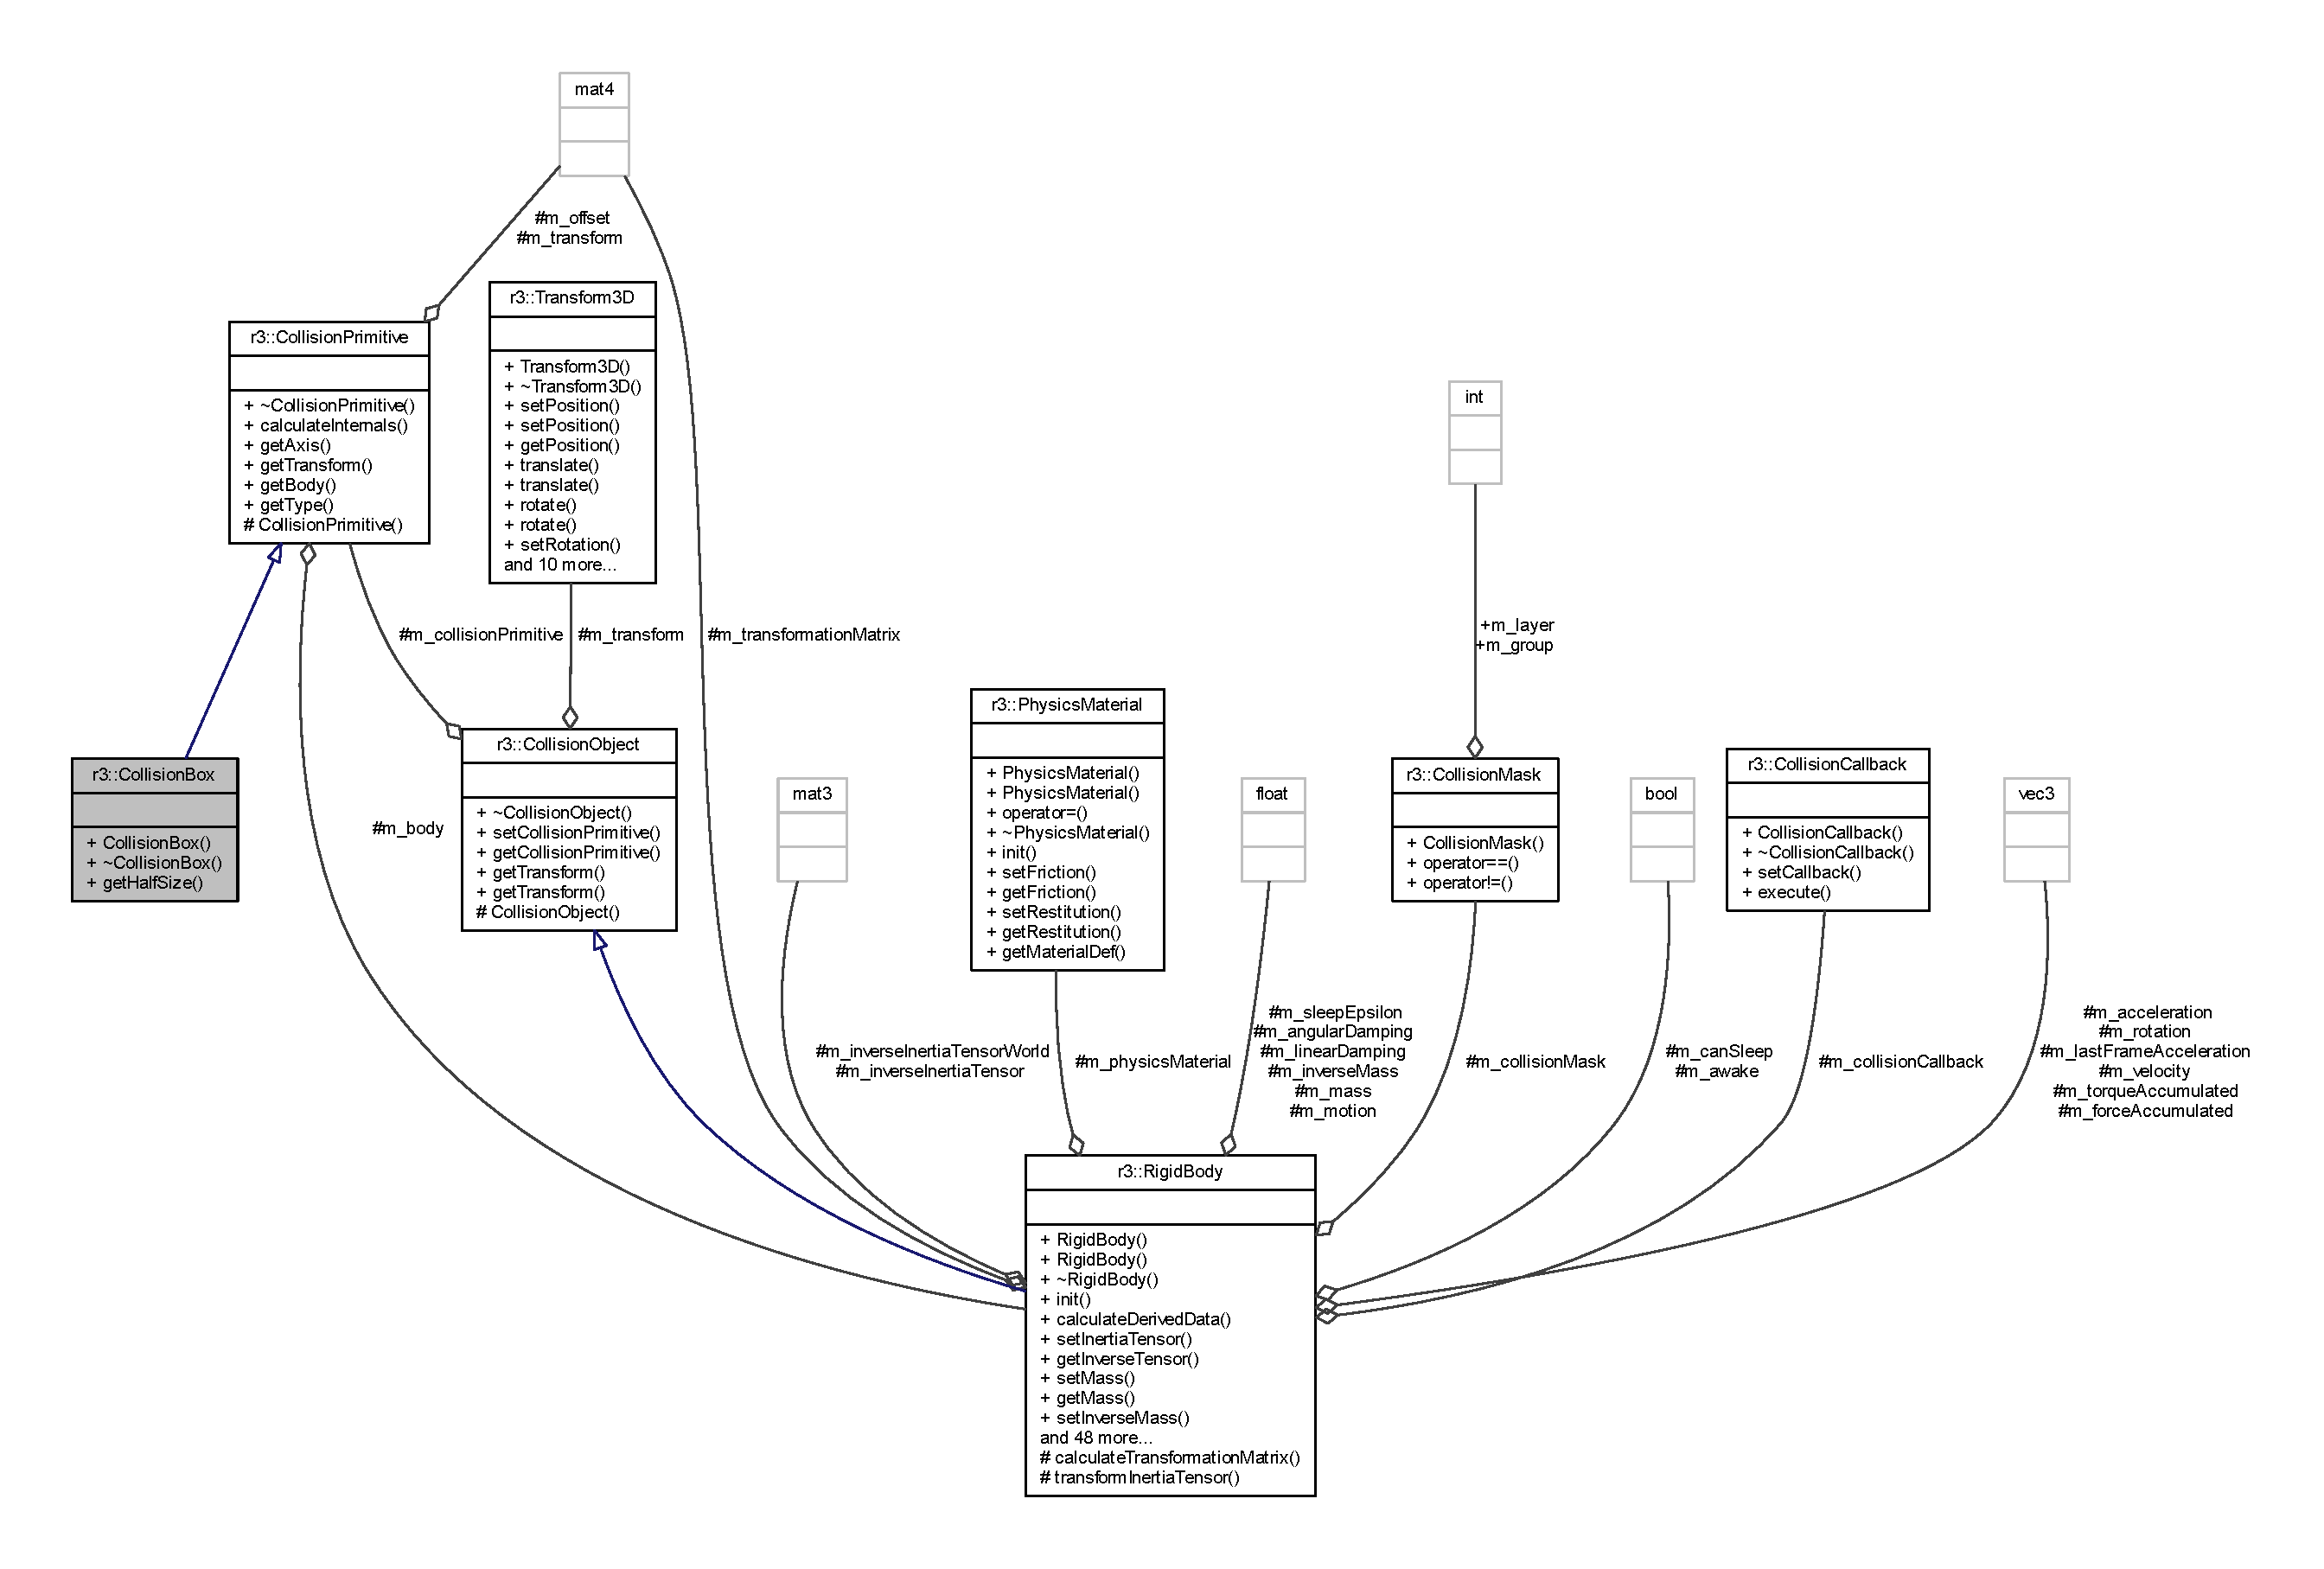
\includegraphics[width=350pt]{classr3_1_1_collision_box__coll__graph}
\end{center}
\end{figure}
\subsection*{Public Member Functions}
\begin{DoxyCompactItemize}
\item 
\mbox{\hyperlink{classr3_1_1_collision_box_af20be9fdcddf3a94d195fabf22d8ad3a}{Collision\+Box}} (\mbox{\hyperlink{classr3_1_1_rigid_body}{Rigid\+Body}} $\ast$body, const glm\+::vec3 \&half\+Sizes, const glm\+::mat4 \&offset=glm\+::mat4(1))
\begin{DoxyCompactList}\small\item\em \mbox{\hyperlink{classr3_1_1_collision_box}{Collision\+Box}} constructor. \end{DoxyCompactList}\item 
\mbox{\hyperlink{classr3_1_1_collision_box_aab1d8f1b7999c61cff10b631305cc4f3}{$\sim$\+Collision\+Box}} ()
\item 
const glm\+::vec3 \& \mbox{\hyperlink{classr3_1_1_collision_box_a2410b400cbf9c41839e4684b00a1da04}{get\+Half\+Size}} () const
\begin{DoxyCompactList}\small\item\em Get the half sizes of the box. \end{DoxyCompactList}\end{DoxyCompactItemize}
\subsection*{Additional Inherited Members}


\subsection{Detailed Description}
\mbox{\hyperlink{classr3_1_1_collision_primitive}{Collision\+Primitive}} that represents a box. 

\subsection{Constructor \& Destructor Documentation}
\mbox{\Hypertarget{classr3_1_1_collision_box_af20be9fdcddf3a94d195fabf22d8ad3a}\label{classr3_1_1_collision_box_af20be9fdcddf3a94d195fabf22d8ad3a}} 
\index{r3\+::\+Collision\+Box@{r3\+::\+Collision\+Box}!Collision\+Box@{Collision\+Box}}
\index{Collision\+Box@{Collision\+Box}!r3\+::\+Collision\+Box@{r3\+::\+Collision\+Box}}
\subsubsection{\texorpdfstring{Collision\+Box()}{CollisionBox()}}
{\footnotesize\ttfamily r3\+::\+Collision\+Box\+::\+Collision\+Box (\begin{DoxyParamCaption}\item[{\mbox{\hyperlink{classr3_1_1_rigid_body}{Rigid\+Body}} $\ast$}]{body,  }\item[{const glm\+::vec3 \&}]{half\+Sizes,  }\item[{const glm\+::mat4 \&}]{offset = {\ttfamily glm\+:\+:mat4(1)} }\end{DoxyParamCaption})\hspace{0.3cm}{\ttfamily [explicit]}}



\mbox{\hyperlink{classr3_1_1_collision_box}{Collision\+Box}} constructor. 


\begin{DoxyParams}{Parameters}
{\em body} & The rigid body represented by this primitive. \\
\hline
{\em half\+Sizes} & The half sizes of the box. \\
\hline
{\em offset} & The offset from the rigid body. \\
\hline
\end{DoxyParams}
\mbox{\Hypertarget{classr3_1_1_collision_box_aab1d8f1b7999c61cff10b631305cc4f3}\label{classr3_1_1_collision_box_aab1d8f1b7999c61cff10b631305cc4f3}} 
\index{r3\+::\+Collision\+Box@{r3\+::\+Collision\+Box}!````~Collision\+Box@{$\sim$\+Collision\+Box}}
\index{````~Collision\+Box@{$\sim$\+Collision\+Box}!r3\+::\+Collision\+Box@{r3\+::\+Collision\+Box}}
\subsubsection{\texorpdfstring{$\sim$\+Collision\+Box()}{~CollisionBox()}}
{\footnotesize\ttfamily r3\+::\+Collision\+Box\+::$\sim$\+Collision\+Box (\begin{DoxyParamCaption}{ }\end{DoxyParamCaption})\hspace{0.3cm}{\ttfamily [default]}}



\subsection{Member Function Documentation}
\mbox{\Hypertarget{classr3_1_1_collision_box_a2410b400cbf9c41839e4684b00a1da04}\label{classr3_1_1_collision_box_a2410b400cbf9c41839e4684b00a1da04}} 
\index{r3\+::\+Collision\+Box@{r3\+::\+Collision\+Box}!get\+Half\+Size@{get\+Half\+Size}}
\index{get\+Half\+Size@{get\+Half\+Size}!r3\+::\+Collision\+Box@{r3\+::\+Collision\+Box}}
\subsubsection{\texorpdfstring{get\+Half\+Size()}{getHalfSize()}}
{\footnotesize\ttfamily const glm\+::vec3 \& r3\+::\+Collision\+Box\+::get\+Half\+Size (\begin{DoxyParamCaption}{ }\end{DoxyParamCaption}) const}



Get the half sizes of the box. 

\begin{DoxyReturn}{Returns}
The half sizes. 
\end{DoxyReturn}


The documentation for this class was generated from the following files\+:\begin{DoxyCompactItemize}
\item 
D\+:/\+Library/\+Documents/\+Job/\+Forschungsmaster/\+Projekte/\+Simulation\+Visualization/\+Rumble3\+D/\+Rumble3\+D/include/\+R3\+D/\+Rigid\+Body\+Engine/\mbox{\hyperlink{_collision_box_8h}{Collision\+Box.\+h}}\item 
D\+:/\+Library/\+Documents/\+Job/\+Forschungsmaster/\+Projekte/\+Simulation\+Visualization/\+Rumble3\+D/\+Rumble3\+D/src/\+Rigid\+Body\+Engine/\mbox{\hyperlink{_collision_box_8cpp}{Collision\+Box.\+cpp}}\end{DoxyCompactItemize}

\hypertarget{classr3_1_1_collision_callback}{}\section{r3\+:\+:Collision\+Callback Class Reference}
\label{classr3_1_1_collision_callback}\index{r3\+::\+Collision\+Callback@{r3\+::\+Collision\+Callback}}


Callback, which gets executed, when two rigid bodies collide.  




{\ttfamily \#include $<$Collision\+Callback.\+h$>$}



Collaboration diagram for r3\+:\+:Collision\+Callback\+:\nopagebreak
\begin{figure}[H]
\begin{center}
\leavevmode
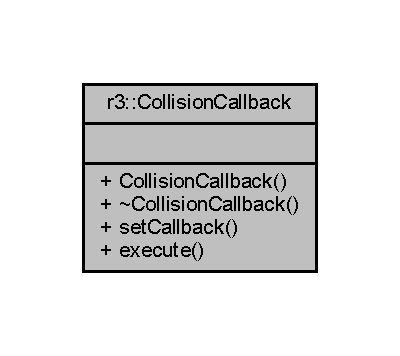
\includegraphics[width=192pt]{classr3_1_1_collision_callback__coll__graph}
\end{center}
\end{figure}
\subsection*{Public Types}
\begin{DoxyCompactItemize}
\item 
using \mbox{\hyperlink{classr3_1_1_collision_callback_afcd5494eafdbd1a0956589b6ec9c0728}{Callback}} = std\+::function$<$ void(\mbox{\hyperlink{classr3_1_1_rigid_body}{Rigid\+Body}} $\ast$, \mbox{\hyperlink{classr3_1_1_rigid_body}{Rigid\+Body}} $\ast$)$>$
\end{DoxyCompactItemize}
\subsection*{Public Member Functions}
\begin{DoxyCompactItemize}
\item 
\mbox{\hyperlink{classr3_1_1_collision_callback_ad18bc4d3c1e63ade9cb9ec420de59591}{Collision\+Callback}} (\mbox{\hyperlink{classr3_1_1_collision_callback_afcd5494eafdbd1a0956589b6ec9c0728}{Callback}} callback=nullptr)
\item 
\mbox{\hyperlink{classr3_1_1_collision_callback_af85a61a2c9b93718f6930bb21e27faa0}{$\sim$\+Collision\+Callback}} ()
\item 
void \mbox{\hyperlink{classr3_1_1_collision_callback_ab6a33e6f074ebd6860f396c3b0a78423}{set\+Callback}} (const \mbox{\hyperlink{classr3_1_1_collision_callback_afcd5494eafdbd1a0956589b6ec9c0728}{Callback}} \&callback)
\begin{DoxyCompactList}\small\item\em Set the currently used callback function. \end{DoxyCompactList}\item 
void \mbox{\hyperlink{classr3_1_1_collision_callback_afe734fe9303efadfdd6c1abc3910c432}{execute}} (\mbox{\hyperlink{classr3_1_1_rigid_body}{Rigid\+Body}} $\ast$rb1, \mbox{\hyperlink{classr3_1_1_rigid_body}{Rigid\+Body}} $\ast$rb2) const
\begin{DoxyCompactList}\small\item\em Execute the underlying callback. \end{DoxyCompactList}\end{DoxyCompactItemize}


\subsection{Detailed Description}
Callback, which gets executed, when two rigid bodies collide. 

\subsection{Member Typedef Documentation}
\mbox{\Hypertarget{classr3_1_1_collision_callback_afcd5494eafdbd1a0956589b6ec9c0728}\label{classr3_1_1_collision_callback_afcd5494eafdbd1a0956589b6ec9c0728}} 
\index{r3\+::\+Collision\+Callback@{r3\+::\+Collision\+Callback}!Callback@{Callback}}
\index{Callback@{Callback}!r3\+::\+Collision\+Callback@{r3\+::\+Collision\+Callback}}
\subsubsection{\texorpdfstring{Callback}{Callback}}
{\footnotesize\ttfamily using \mbox{\hyperlink{classr3_1_1_collision_callback_afcd5494eafdbd1a0956589b6ec9c0728}{r3\+::\+Collision\+Callback\+::\+Callback}} =  std\+::function$<$void(\mbox{\hyperlink{classr3_1_1_rigid_body}{Rigid\+Body}}$\ast$, \mbox{\hyperlink{classr3_1_1_rigid_body}{Rigid\+Body}}$\ast$)$>$}



\subsection{Constructor \& Destructor Documentation}
\mbox{\Hypertarget{classr3_1_1_collision_callback_ad18bc4d3c1e63ade9cb9ec420de59591}\label{classr3_1_1_collision_callback_ad18bc4d3c1e63ade9cb9ec420de59591}} 
\index{r3\+::\+Collision\+Callback@{r3\+::\+Collision\+Callback}!Collision\+Callback@{Collision\+Callback}}
\index{Collision\+Callback@{Collision\+Callback}!r3\+::\+Collision\+Callback@{r3\+::\+Collision\+Callback}}
\subsubsection{\texorpdfstring{Collision\+Callback()}{CollisionCallback()}}
{\footnotesize\ttfamily r3\+::\+Collision\+Callback\+::\+Collision\+Callback (\begin{DoxyParamCaption}\item[{\mbox{\hyperlink{classr3_1_1_collision_callback_afcd5494eafdbd1a0956589b6ec9c0728}{Callback}}}]{callback = {\ttfamily nullptr} }\end{DoxyParamCaption})\hspace{0.3cm}{\ttfamily [explicit]}}

\mbox{\Hypertarget{classr3_1_1_collision_callback_af85a61a2c9b93718f6930bb21e27faa0}\label{classr3_1_1_collision_callback_af85a61a2c9b93718f6930bb21e27faa0}} 
\index{r3\+::\+Collision\+Callback@{r3\+::\+Collision\+Callback}!````~Collision\+Callback@{$\sim$\+Collision\+Callback}}
\index{````~Collision\+Callback@{$\sim$\+Collision\+Callback}!r3\+::\+Collision\+Callback@{r3\+::\+Collision\+Callback}}
\subsubsection{\texorpdfstring{$\sim$\+Collision\+Callback()}{~CollisionCallback()}}
{\footnotesize\ttfamily r3\+::\+Collision\+Callback\+::$\sim$\+Collision\+Callback (\begin{DoxyParamCaption}{ }\end{DoxyParamCaption})\hspace{0.3cm}{\ttfamily [default]}}



\subsection{Member Function Documentation}
\mbox{\Hypertarget{classr3_1_1_collision_callback_afe734fe9303efadfdd6c1abc3910c432}\label{classr3_1_1_collision_callback_afe734fe9303efadfdd6c1abc3910c432}} 
\index{r3\+::\+Collision\+Callback@{r3\+::\+Collision\+Callback}!execute@{execute}}
\index{execute@{execute}!r3\+::\+Collision\+Callback@{r3\+::\+Collision\+Callback}}
\subsubsection{\texorpdfstring{execute()}{execute()}}
{\footnotesize\ttfamily void r3\+::\+Collision\+Callback\+::execute (\begin{DoxyParamCaption}\item[{\mbox{\hyperlink{classr3_1_1_rigid_body}{Rigid\+Body}} $\ast$}]{rb1,  }\item[{\mbox{\hyperlink{classr3_1_1_rigid_body}{Rigid\+Body}} $\ast$}]{rb2 }\end{DoxyParamCaption}) const}



Execute the underlying callback. 

\mbox{\Hypertarget{classr3_1_1_collision_callback_ab6a33e6f074ebd6860f396c3b0a78423}\label{classr3_1_1_collision_callback_ab6a33e6f074ebd6860f396c3b0a78423}} 
\index{r3\+::\+Collision\+Callback@{r3\+::\+Collision\+Callback}!set\+Callback@{set\+Callback}}
\index{set\+Callback@{set\+Callback}!r3\+::\+Collision\+Callback@{r3\+::\+Collision\+Callback}}
\subsubsection{\texorpdfstring{set\+Callback()}{setCallback()}}
{\footnotesize\ttfamily void r3\+::\+Collision\+Callback\+::set\+Callback (\begin{DoxyParamCaption}\item[{const \mbox{\hyperlink{classr3_1_1_collision_callback_afcd5494eafdbd1a0956589b6ec9c0728}{Callback}} \&}]{callback }\end{DoxyParamCaption})}



Set the currently used callback function. 



The documentation for this class was generated from the following files\+:\begin{DoxyCompactItemize}
\item 
D\+:/\+Library/\+Documents/\+Job/\+Forschungsmaster/\+Projekte/\+Simulation\+Visualization/\+Rumble3\+D/\+Rumble3\+D/include/\+R3\+D/\+Rigid\+Body\+Engine/\mbox{\hyperlink{_collision_callback_8h}{Collision\+Callback.\+h}}\item 
D\+:/\+Library/\+Documents/\+Job/\+Forschungsmaster/\+Projekte/\+Simulation\+Visualization/\+Rumble3\+D/\+Rumble3\+D/src/\+Rigid\+Body\+Engine/\mbox{\hyperlink{_collision_callback_8cpp}{Collision\+Callback.\+cpp}}\end{DoxyCompactItemize}

\hypertarget{classr3_1_1_collision_data}{}\doxysection{r3\+::Collision\+Data Class Reference}
\label{classr3_1_1_collision_data}\index{r3::CollisionData@{r3::CollisionData}}


{\ttfamily \#include $<$Collision\+Data.\+h$>$}



Collaboration diagram for r3\+::Collision\+Data\+:\nopagebreak
\begin{figure}[H]
\begin{center}
\leavevmode
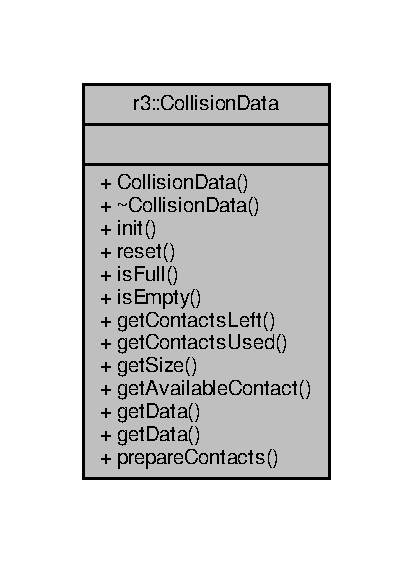
\includegraphics[width=198pt]{classr3_1_1_collision_data__coll__graph}
\end{center}
\end{figure}
\doxysubsection*{Public Member Functions}
\begin{DoxyCompactItemize}
\item 
\mbox{\hyperlink{classr3_1_1_collision_data_a439100db9ec5b734e2f0b778d2f97cce}{Collision\+Data}} (unsigned int contacts\+Max=1000, int iterations=0)
\item 
\mbox{\hyperlink{classr3_1_1_collision_data_a3fd93aed7add6b43bc6b3dca59d638f2}{$\sim$\+Collision\+Data}} ()
\item 
void \mbox{\hyperlink{classr3_1_1_collision_data_a2af69fd6da492254b1a134d4ef82efce}{init}} (int contacts\+Max, int iterations)
\item 
void \mbox{\hyperlink{classr3_1_1_collision_data_af74822ca6881f5ab54447a73ac26d7fd}{reset}} ()
\item 
bool \mbox{\hyperlink{classr3_1_1_collision_data_aebb099e77b79235942a9c0166eb66a78}{is\+Full}} () const
\begin{DoxyCompactList}\small\item\em Check if there is no more room for new contacts. \end{DoxyCompactList}\item 
bool \mbox{\hyperlink{classr3_1_1_collision_data_a3b97a4828252625e891c939ad7ce0064}{is\+Empty}} () const
\begin{DoxyCompactList}\small\item\em Check if no contacts are used. \end{DoxyCompactList}\item 
int \mbox{\hyperlink{classr3_1_1_collision_data_a13e8ade4bbbbc63a1437de9371fea879}{get\+Contacts\+Left}} () const
\begin{DoxyCompactList}\small\item\em Check how many contacts can still be inserted. \end{DoxyCompactList}\item 
int \mbox{\hyperlink{classr3_1_1_collision_data_aaf0e65914133cd35cc32224df851561e}{get\+Contacts\+Used}} () const
\begin{DoxyCompactList}\small\item\em Check how many contacts have been inserted. \end{DoxyCompactList}\item 
int \mbox{\hyperlink{classr3_1_1_collision_data_ad0898e21e34b4558dbdd68dd115c49d8}{get\+Size}} () const
\begin{DoxyCompactList}\small\item\em Get the maximal number of contacts. \end{DoxyCompactList}\item 
\mbox{\hyperlink{classr3_1_1_contact}{Contact}} $\ast$ \mbox{\hyperlink{classr3_1_1_collision_data_ad0e0b85004905b48a8faf7be34bdf305}{get\+Available\+Contact}} ()
\begin{DoxyCompactList}\small\item\em Get the next available contact. Automatically uses it! \end{DoxyCompactList}\item 
std\+::vector$<$ \mbox{\hyperlink{classr3_1_1_contact}{Contact}} $>$ \& \mbox{\hyperlink{classr3_1_1_collision_data_acb1bb23e8d0f37f0ebc39e8f7642419f}{get\+Data}} ()
\begin{DoxyCompactList}\small\item\em Get all contacts (only valid to a certain position) \end{DoxyCompactList}\item 
const std\+::vector$<$ \mbox{\hyperlink{classr3_1_1_contact}{Contact}} $>$ \& \mbox{\hyperlink{classr3_1_1_collision_data_ab31745ebb708c1d04e22bcfb385e663f}{get\+Data}} () const
\begin{DoxyCompactList}\small\item\em Get all contacts (only valid to a certain position) \end{DoxyCompactList}\item 
void \mbox{\hyperlink{classr3_1_1_collision_data_a7a8dcf7d0b2cdd99d9c96dabc2a4fbc9}{prepare\+Contacts}} (\mbox{\hyperlink{namespacer3_ab2016b3e3f743fb735afce242f0dc1eb}{real}} time\+Delta)
\end{DoxyCompactItemize}


\doxysubsection{Constructor \& Destructor Documentation}
\mbox{\Hypertarget{classr3_1_1_collision_data_a439100db9ec5b734e2f0b778d2f97cce}\label{classr3_1_1_collision_data_a439100db9ec5b734e2f0b778d2f97cce}} 
\index{r3::CollisionData@{r3::CollisionData}!CollisionData@{CollisionData}}
\index{CollisionData@{CollisionData}!r3::CollisionData@{r3::CollisionData}}
\doxysubsubsection{\texorpdfstring{CollisionData()}{CollisionData()}}
{\footnotesize\ttfamily r3\+::\+Collision\+Data\+::\+Collision\+Data (\begin{DoxyParamCaption}\item[{unsigned int}]{contacts\+Max = {\ttfamily 1000},  }\item[{int}]{iterations = {\ttfamily 0} }\end{DoxyParamCaption})\hspace{0.3cm}{\ttfamily [explicit]}}

\mbox{\Hypertarget{classr3_1_1_collision_data_a3fd93aed7add6b43bc6b3dca59d638f2}\label{classr3_1_1_collision_data_a3fd93aed7add6b43bc6b3dca59d638f2}} 
\index{r3::CollisionData@{r3::CollisionData}!````~CollisionData@{$\sim$CollisionData}}
\index{````~CollisionData@{$\sim$CollisionData}!r3::CollisionData@{r3::CollisionData}}
\doxysubsubsection{\texorpdfstring{$\sim$CollisionData()}{~CollisionData()}}
{\footnotesize\ttfamily r3\+::\+Collision\+Data\+::$\sim$\+Collision\+Data (\begin{DoxyParamCaption}{ }\end{DoxyParamCaption})\hspace{0.3cm}{\ttfamily [default]}}



\doxysubsection{Member Function Documentation}
\mbox{\Hypertarget{classr3_1_1_collision_data_ad0e0b85004905b48a8faf7be34bdf305}\label{classr3_1_1_collision_data_ad0e0b85004905b48a8faf7be34bdf305}} 
\index{r3::CollisionData@{r3::CollisionData}!getAvailableContact@{getAvailableContact}}
\index{getAvailableContact@{getAvailableContact}!r3::CollisionData@{r3::CollisionData}}
\doxysubsubsection{\texorpdfstring{getAvailableContact()}{getAvailableContact()}}
{\footnotesize\ttfamily \mbox{\hyperlink{classr3_1_1_contact}{Contact}} $\ast$ r3\+::\+Collision\+Data\+::get\+Available\+Contact (\begin{DoxyParamCaption}{ }\end{DoxyParamCaption})}



Get the next available contact. Automatically uses it! 

\begin{DoxyReturn}{Returns}
nullptr if all contacts are used, a available contact otherwise. 
\end{DoxyReturn}
\mbox{\Hypertarget{classr3_1_1_collision_data_a13e8ade4bbbbc63a1437de9371fea879}\label{classr3_1_1_collision_data_a13e8ade4bbbbc63a1437de9371fea879}} 
\index{r3::CollisionData@{r3::CollisionData}!getContactsLeft@{getContactsLeft}}
\index{getContactsLeft@{getContactsLeft}!r3::CollisionData@{r3::CollisionData}}
\doxysubsubsection{\texorpdfstring{getContactsLeft()}{getContactsLeft()}}
{\footnotesize\ttfamily int r3\+::\+Collision\+Data\+::get\+Contacts\+Left (\begin{DoxyParamCaption}{ }\end{DoxyParamCaption}) const}



Check how many contacts can still be inserted. 

\mbox{\Hypertarget{classr3_1_1_collision_data_aaf0e65914133cd35cc32224df851561e}\label{classr3_1_1_collision_data_aaf0e65914133cd35cc32224df851561e}} 
\index{r3::CollisionData@{r3::CollisionData}!getContactsUsed@{getContactsUsed}}
\index{getContactsUsed@{getContactsUsed}!r3::CollisionData@{r3::CollisionData}}
\doxysubsubsection{\texorpdfstring{getContactsUsed()}{getContactsUsed()}}
{\footnotesize\ttfamily int r3\+::\+Collision\+Data\+::get\+Contacts\+Used (\begin{DoxyParamCaption}{ }\end{DoxyParamCaption}) const}



Check how many contacts have been inserted. 

\mbox{\Hypertarget{classr3_1_1_collision_data_acb1bb23e8d0f37f0ebc39e8f7642419f}\label{classr3_1_1_collision_data_acb1bb23e8d0f37f0ebc39e8f7642419f}} 
\index{r3::CollisionData@{r3::CollisionData}!getData@{getData}}
\index{getData@{getData}!r3::CollisionData@{r3::CollisionData}}
\doxysubsubsection{\texorpdfstring{getData()}{getData()}\hspace{0.1cm}{\footnotesize\ttfamily [1/2]}}
{\footnotesize\ttfamily std\+::vector$<$ \mbox{\hyperlink{classr3_1_1_contact}{Contact}} $>$ \& r3\+::\+Collision\+Data\+::get\+Data (\begin{DoxyParamCaption}{ }\end{DoxyParamCaption})}



Get all contacts (only valid to a certain position) 

\mbox{\Hypertarget{classr3_1_1_collision_data_ab31745ebb708c1d04e22bcfb385e663f}\label{classr3_1_1_collision_data_ab31745ebb708c1d04e22bcfb385e663f}} 
\index{r3::CollisionData@{r3::CollisionData}!getData@{getData}}
\index{getData@{getData}!r3::CollisionData@{r3::CollisionData}}
\doxysubsubsection{\texorpdfstring{getData()}{getData()}\hspace{0.1cm}{\footnotesize\ttfamily [2/2]}}
{\footnotesize\ttfamily const std\+::vector$<$ \mbox{\hyperlink{classr3_1_1_contact}{Contact}} $>$ \& r3\+::\+Collision\+Data\+::get\+Data (\begin{DoxyParamCaption}{ }\end{DoxyParamCaption}) const}



Get all contacts (only valid to a certain position) 

\mbox{\Hypertarget{classr3_1_1_collision_data_ad0898e21e34b4558dbdd68dd115c49d8}\label{classr3_1_1_collision_data_ad0898e21e34b4558dbdd68dd115c49d8}} 
\index{r3::CollisionData@{r3::CollisionData}!getSize@{getSize}}
\index{getSize@{getSize}!r3::CollisionData@{r3::CollisionData}}
\doxysubsubsection{\texorpdfstring{getSize()}{getSize()}}
{\footnotesize\ttfamily int r3\+::\+Collision\+Data\+::get\+Size (\begin{DoxyParamCaption}{ }\end{DoxyParamCaption}) const}



Get the maximal number of contacts. 

\mbox{\Hypertarget{classr3_1_1_collision_data_a2af69fd6da492254b1a134d4ef82efce}\label{classr3_1_1_collision_data_a2af69fd6da492254b1a134d4ef82efce}} 
\index{r3::CollisionData@{r3::CollisionData}!init@{init}}
\index{init@{init}!r3::CollisionData@{r3::CollisionData}}
\doxysubsubsection{\texorpdfstring{init()}{init()}}
{\footnotesize\ttfamily void r3\+::\+Collision\+Data\+::init (\begin{DoxyParamCaption}\item[{int}]{contacts\+Max,  }\item[{int}]{iterations }\end{DoxyParamCaption})}

\mbox{\Hypertarget{classr3_1_1_collision_data_a3b97a4828252625e891c939ad7ce0064}\label{classr3_1_1_collision_data_a3b97a4828252625e891c939ad7ce0064}} 
\index{r3::CollisionData@{r3::CollisionData}!isEmpty@{isEmpty}}
\index{isEmpty@{isEmpty}!r3::CollisionData@{r3::CollisionData}}
\doxysubsubsection{\texorpdfstring{isEmpty()}{isEmpty()}}
{\footnotesize\ttfamily bool r3\+::\+Collision\+Data\+::is\+Empty (\begin{DoxyParamCaption}{ }\end{DoxyParamCaption}) const}



Check if no contacts are used. 

\mbox{\Hypertarget{classr3_1_1_collision_data_aebb099e77b79235942a9c0166eb66a78}\label{classr3_1_1_collision_data_aebb099e77b79235942a9c0166eb66a78}} 
\index{r3::CollisionData@{r3::CollisionData}!isFull@{isFull}}
\index{isFull@{isFull}!r3::CollisionData@{r3::CollisionData}}
\doxysubsubsection{\texorpdfstring{isFull()}{isFull()}}
{\footnotesize\ttfamily bool r3\+::\+Collision\+Data\+::is\+Full (\begin{DoxyParamCaption}{ }\end{DoxyParamCaption}) const}



Check if there is no more room for new contacts. 

\mbox{\Hypertarget{classr3_1_1_collision_data_a7a8dcf7d0b2cdd99d9c96dabc2a4fbc9}\label{classr3_1_1_collision_data_a7a8dcf7d0b2cdd99d9c96dabc2a4fbc9}} 
\index{r3::CollisionData@{r3::CollisionData}!prepareContacts@{prepareContacts}}
\index{prepareContacts@{prepareContacts}!r3::CollisionData@{r3::CollisionData}}
\doxysubsubsection{\texorpdfstring{prepareContacts()}{prepareContacts()}}
{\footnotesize\ttfamily void r3\+::\+Collision\+Data\+::prepare\+Contacts (\begin{DoxyParamCaption}\item[{\mbox{\hyperlink{namespacer3_ab2016b3e3f743fb735afce242f0dc1eb}{real}}}]{time\+Delta }\end{DoxyParamCaption})}

\mbox{\Hypertarget{classr3_1_1_collision_data_af74822ca6881f5ab54447a73ac26d7fd}\label{classr3_1_1_collision_data_af74822ca6881f5ab54447a73ac26d7fd}} 
\index{r3::CollisionData@{r3::CollisionData}!reset@{reset}}
\index{reset@{reset}!r3::CollisionData@{r3::CollisionData}}
\doxysubsubsection{\texorpdfstring{reset()}{reset()}}
{\footnotesize\ttfamily void r3\+::\+Collision\+Data\+::reset (\begin{DoxyParamCaption}{ }\end{DoxyParamCaption})}



The documentation for this class was generated from the following files\+:\begin{DoxyCompactItemize}
\item 
/home/nelaty/\+Development/\+Repositories/\+Rumble3\+D/include/\+R3\+D/\+Rigid\+Body\+Engine/\+Collision\+Detection/\mbox{\hyperlink{_collision_data_8h}{Collision\+Data.\+h}}\item 
/home/nelaty/\+Development/\+Repositories/\+Rumble3\+D/src/\+Rigid\+Body\+Engine/\+Collision\+Detection/\mbox{\hyperlink{_collision_data_8cpp}{Collision\+Data.\+cpp}}\end{DoxyCompactItemize}

\hypertarget{classr3_1_1_collision_detector}{}\section{r3\+:\+:Collision\+Detector Class Reference}
\label{classr3_1_1_collision_detector}\index{r3\+::\+Collision\+Detector@{r3\+::\+Collision\+Detector}}


{\ttfamily \#include $<$Collision\+Detector.\+h$>$}



Collaboration diagram for r3\+:\+:Collision\+Detector\+:\nopagebreak
\begin{figure}[H]
\begin{center}
\leavevmode
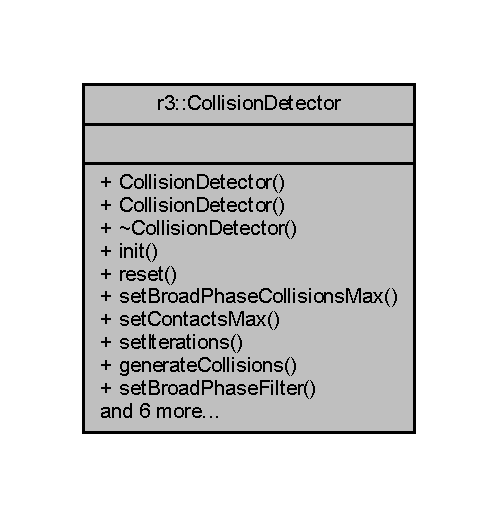
\includegraphics[width=239pt]{classr3_1_1_collision_detector__coll__graph}
\end{center}
\end{figure}
\subsection*{Public Types}
\begin{DoxyCompactItemize}
\item 
using \mbox{\hyperlink{classr3_1_1_collision_detector_aa8ed51d53c6f6ce545c93ad0e356d6de}{Broad\+Phase\+Filter\+\_\+\+Ptr}} = std\+::unique\+\_\+ptr$<$ \mbox{\hyperlink{classr3_1_1_i_broad_phase_filter}{I\+Broad\+Phase\+Filter}} $>$
\item 
using \mbox{\hyperlink{classr3_1_1_collision_detector_a8337c2c23ec77350b65977e043c07827}{Intermediate\+Phase\+Filter\+\_\+\+Ptr}} = std\+::unique\+\_\+ptr$<$ \mbox{\hyperlink{classr3_1_1_i_intermediate_phase_filter}{I\+Intermediate\+Phase\+Filter}} $>$
\item 
using \mbox{\hyperlink{classr3_1_1_collision_detector_a094cc287cba14d5a063cfca41e667008}{Narrow\+Phase\+Filter\+\_\+\+Ptr}} = std\+::unique\+\_\+ptr$<$ \mbox{\hyperlink{classr3_1_1_i_narrow_phase_filter}{I\+Narrow\+Phase\+Filter}} $>$
\end{DoxyCompactItemize}
\subsection*{Public Member Functions}
\begin{DoxyCompactItemize}
\item 
\mbox{\hyperlink{classr3_1_1_collision_detector_a8eaf42ee83c8bee06bc06601ec32c612}{Collision\+Detector}} (unsigned broad\+Phase\+Collisions=1000000, unsigned contacts\+Max=1000, unsigned iterations=2000)
\begin{DoxyCompactList}\small\item\em \mbox{\hyperlink{classr3_1_1_collision_detector}{Collision\+Detector}} constructor. \end{DoxyCompactList}\item 
\mbox{\hyperlink{classr3_1_1_collision_detector_ad44d67dd15e661d0e135016c89a7c9a4}{Collision\+Detector}} (const \mbox{\hyperlink{classr3_1_1_collision_detector}{Collision\+Detector}} \&)=delete
\item 
\mbox{\hyperlink{classr3_1_1_collision_detector_ab45ac57f6ab9bcab367e104e9423722a}{$\sim$\+Collision\+Detector}} ()
\item 
void \mbox{\hyperlink{classr3_1_1_collision_detector_a252e876b389dae66368afa210b93f31e}{init}} (unsigned broad\+Phase\+Collisions=1000000, unsigned contacts\+Max=1000, unsigned iterations=2000)
\begin{DoxyCompactList}\small\item\em Set the number of used contacts and iterations. \end{DoxyCompactList}\item 
void \mbox{\hyperlink{classr3_1_1_collision_detector_a8f9f9e0ecc67d950e79d024803dc916b}{reset}} ()
\begin{DoxyCompactList}\small\item\em Reset previously calculated collisions. \end{DoxyCompactList}\item 
void \mbox{\hyperlink{classr3_1_1_collision_detector_a386e4e4027a98c154423c8aea9079138}{set\+Broad\+Phase\+Collisions\+Max}} (int count)
\begin{DoxyCompactList}\small\item\em Set the maximal number of collision pairs created in the broad and intermediate phases. \end{DoxyCompactList}\item 
void \mbox{\hyperlink{classr3_1_1_collision_detector_a1920971e75d79df7806a8d803a010e62}{set\+Contacts\+Max}} (int count)
\begin{DoxyCompactList}\small\item\em Set the maximal number of contacts created in the narrow phase. \end{DoxyCompactList}\item 
void \mbox{\hyperlink{classr3_1_1_collision_detector_a4d6081592ca35150cd6c8fe0d551c64d}{set\+Iterations}} (int iterations)
\begin{DoxyCompactList}\small\item\em Set the maximal number of iterations used. \end{DoxyCompactList}\item 
\mbox{\hyperlink{classr3_1_1_collision_data}{Collision\+Data}} \& \mbox{\hyperlink{classr3_1_1_collision_detector_a58a1bd9705f241e4c137458bed35f596}{generate\+Collisions}} (const std\+::vector$<$ \mbox{\hyperlink{classr3_1_1_rigid_body}{Rigid\+Body}} $\ast$$>$ \&rigid\+Bodies)
\begin{DoxyCompactList}\small\item\em Generate a number of contacts for the given rigid bodies with the help of the current filters. \end{DoxyCompactList}\item 
void \mbox{\hyperlink{classr3_1_1_collision_detector_a2184ca2db73a6446cf028e3b742c7cc4}{set\+Broad\+Phase\+Filter}} (\mbox{\hyperlink{classr3_1_1_collision_detector_aa8ed51d53c6f6ce545c93ad0e356d6de}{Broad\+Phase\+Filter\+\_\+\+Ptr}} filter)
\begin{DoxyCompactList}\small\item\em Set the currently used broad phase filter. \end{DoxyCompactList}\item 
\mbox{\hyperlink{classr3_1_1_i_broad_phase_filter}{I\+Broad\+Phase\+Filter}} $\ast$ \mbox{\hyperlink{classr3_1_1_collision_detector_aa4d1c9560f806496b2215ddc623a1387}{get\+Broad\+Phase\+Filter}} () const
\begin{DoxyCompactList}\small\item\em Get the currently used broad phase filter. \end{DoxyCompactList}\item 
\mbox{\hyperlink{classr3_1_1_i_intermediate_phase_filter}{I\+Intermediate\+Phase\+Filter}} $\ast$ \mbox{\hyperlink{classr3_1_1_collision_detector_a804d66d43502a2b113aa1e8c302cebc7}{add\+Intermediate\+Phase\+Filter}} (\mbox{\hyperlink{classr3_1_1_collision_detector_a8337c2c23ec77350b65977e043c07827}{Intermediate\+Phase\+Filter\+\_\+\+Ptr}} filter)
\begin{DoxyCompactList}\small\item\em Add a new intermediate phase filter, which will be executed after all currently registered intermediate phase filters. \end{DoxyCompactList}\item 
\mbox{\hyperlink{classr3_1_1_collision_detector_a8337c2c23ec77350b65977e043c07827}{Intermediate\+Phase\+Filter\+\_\+\+Ptr}} \mbox{\hyperlink{classr3_1_1_collision_detector_aff67a43ffc0f74ada2193f46aa3ea1fd}{remove\+Intermediate\+Phase\+Filter}} (\mbox{\hyperlink{classr3_1_1_i_intermediate_phase_filter}{I\+Intermediate\+Phase\+Filter}} $\ast$filter)
\item 
void \mbox{\hyperlink{classr3_1_1_collision_detector_a780e977afd65d4a41863e712f9acb63f}{remove\+All\+Intermediate\+Phase\+Filters}} ()
\begin{DoxyCompactList}\small\item\em Clears the list of all currently registered intermediate phase filters. \end{DoxyCompactList}\item 
void \mbox{\hyperlink{classr3_1_1_collision_detector_a98f6ab749622d7fcffbdc0dcf59cfa75}{set\+Narrow\+Phase\+Filter}} (\mbox{\hyperlink{classr3_1_1_collision_detector_a094cc287cba14d5a063cfca41e667008}{Narrow\+Phase\+Filter\+\_\+\+Ptr}} filter)
\begin{DoxyCompactList}\small\item\em Set the currently used narrow phase filter. \end{DoxyCompactList}\item 
\mbox{\hyperlink{classr3_1_1_i_narrow_phase_filter}{I\+Narrow\+Phase\+Filter}} $\ast$ \mbox{\hyperlink{classr3_1_1_collision_detector_aa43b5d1332028d15a3c9af1ec4cd4312}{get\+Narrow\+Phase\+Filter}} () const
\begin{DoxyCompactList}\small\item\em Get the currently used narrow phase filter. \end{DoxyCompactList}\end{DoxyCompactItemize}


\subsection{Detailed Description}
The \mbox{\hyperlink{classr3_1_1_collision_detector}{Collision\+Detector}} acts as a batch controller (batch sequential). It executes collision detection filters (programs) in a specific order to generate contacts. 

\subsection{Member Typedef Documentation}
\mbox{\Hypertarget{classr3_1_1_collision_detector_aa8ed51d53c6f6ce545c93ad0e356d6de}\label{classr3_1_1_collision_detector_aa8ed51d53c6f6ce545c93ad0e356d6de}} 
\index{r3\+::\+Collision\+Detector@{r3\+::\+Collision\+Detector}!Broad\+Phase\+Filter\+\_\+\+Ptr@{Broad\+Phase\+Filter\+\_\+\+Ptr}}
\index{Broad\+Phase\+Filter\+\_\+\+Ptr@{Broad\+Phase\+Filter\+\_\+\+Ptr}!r3\+::\+Collision\+Detector@{r3\+::\+Collision\+Detector}}
\subsubsection{\texorpdfstring{Broad\+Phase\+Filter\+\_\+\+Ptr}{BroadPhaseFilter\_Ptr}}
{\footnotesize\ttfamily using \mbox{\hyperlink{classr3_1_1_collision_detector_aa8ed51d53c6f6ce545c93ad0e356d6de}{r3\+::\+Collision\+Detector\+::\+Broad\+Phase\+Filter\+\_\+\+Ptr}} =  std\+::unique\+\_\+ptr$<$\mbox{\hyperlink{classr3_1_1_i_broad_phase_filter}{I\+Broad\+Phase\+Filter}}$>$}

\mbox{\Hypertarget{classr3_1_1_collision_detector_a8337c2c23ec77350b65977e043c07827}\label{classr3_1_1_collision_detector_a8337c2c23ec77350b65977e043c07827}} 
\index{r3\+::\+Collision\+Detector@{r3\+::\+Collision\+Detector}!Intermediate\+Phase\+Filter\+\_\+\+Ptr@{Intermediate\+Phase\+Filter\+\_\+\+Ptr}}
\index{Intermediate\+Phase\+Filter\+\_\+\+Ptr@{Intermediate\+Phase\+Filter\+\_\+\+Ptr}!r3\+::\+Collision\+Detector@{r3\+::\+Collision\+Detector}}
\subsubsection{\texorpdfstring{Intermediate\+Phase\+Filter\+\_\+\+Ptr}{IntermediatePhaseFilter\_Ptr}}
{\footnotesize\ttfamily using \mbox{\hyperlink{classr3_1_1_collision_detector_a8337c2c23ec77350b65977e043c07827}{r3\+::\+Collision\+Detector\+::\+Intermediate\+Phase\+Filter\+\_\+\+Ptr}} =  std\+::unique\+\_\+ptr$<$\mbox{\hyperlink{classr3_1_1_i_intermediate_phase_filter}{I\+Intermediate\+Phase\+Filter}}$>$}

\mbox{\Hypertarget{classr3_1_1_collision_detector_a094cc287cba14d5a063cfca41e667008}\label{classr3_1_1_collision_detector_a094cc287cba14d5a063cfca41e667008}} 
\index{r3\+::\+Collision\+Detector@{r3\+::\+Collision\+Detector}!Narrow\+Phase\+Filter\+\_\+\+Ptr@{Narrow\+Phase\+Filter\+\_\+\+Ptr}}
\index{Narrow\+Phase\+Filter\+\_\+\+Ptr@{Narrow\+Phase\+Filter\+\_\+\+Ptr}!r3\+::\+Collision\+Detector@{r3\+::\+Collision\+Detector}}
\subsubsection{\texorpdfstring{Narrow\+Phase\+Filter\+\_\+\+Ptr}{NarrowPhaseFilter\_Ptr}}
{\footnotesize\ttfamily using \mbox{\hyperlink{classr3_1_1_collision_detector_a094cc287cba14d5a063cfca41e667008}{r3\+::\+Collision\+Detector\+::\+Narrow\+Phase\+Filter\+\_\+\+Ptr}} =  std\+::unique\+\_\+ptr$<$\mbox{\hyperlink{classr3_1_1_i_narrow_phase_filter}{I\+Narrow\+Phase\+Filter}}$>$}



\subsection{Constructor \& Destructor Documentation}
\mbox{\Hypertarget{classr3_1_1_collision_detector_a8eaf42ee83c8bee06bc06601ec32c612}\label{classr3_1_1_collision_detector_a8eaf42ee83c8bee06bc06601ec32c612}} 
\index{r3\+::\+Collision\+Detector@{r3\+::\+Collision\+Detector}!Collision\+Detector@{Collision\+Detector}}
\index{Collision\+Detector@{Collision\+Detector}!r3\+::\+Collision\+Detector@{r3\+::\+Collision\+Detector}}
\subsubsection{\texorpdfstring{Collision\+Detector()}{CollisionDetector()}\hspace{0.1cm}{\footnotesize\ttfamily [1/2]}}
{\footnotesize\ttfamily r3\+::\+Collision\+Detector\+::\+Collision\+Detector (\begin{DoxyParamCaption}\item[{unsigned}]{broad\+Phase\+Collisions = {\ttfamily 1000000},  }\item[{unsigned}]{contacts\+Max = {\ttfamily 1000},  }\item[{unsigned}]{iterations = {\ttfamily 2000} }\end{DoxyParamCaption})\hspace{0.3cm}{\ttfamily [explicit]}}



\mbox{\hyperlink{classr3_1_1_collision_detector}{Collision\+Detector}} constructor. 


\begin{DoxyParams}{Parameters}
{\em broad\+Phase\+Collisions} & The maximal number of collision that can be generated in the broad phase. \\
\hline
{\em contacts\+Max} & The maximal number of contacts that can be generated in the narrow phase. \\
\hline
{\em iterations} & The maximal number of iterations that can be used in contact generation. \\
\hline
\end{DoxyParams}
\mbox{\Hypertarget{classr3_1_1_collision_detector_ad44d67dd15e661d0e135016c89a7c9a4}\label{classr3_1_1_collision_detector_ad44d67dd15e661d0e135016c89a7c9a4}} 
\index{r3\+::\+Collision\+Detector@{r3\+::\+Collision\+Detector}!Collision\+Detector@{Collision\+Detector}}
\index{Collision\+Detector@{Collision\+Detector}!r3\+::\+Collision\+Detector@{r3\+::\+Collision\+Detector}}
\subsubsection{\texorpdfstring{Collision\+Detector()}{CollisionDetector()}\hspace{0.1cm}{\footnotesize\ttfamily [2/2]}}
{\footnotesize\ttfamily r3\+::\+Collision\+Detector\+::\+Collision\+Detector (\begin{DoxyParamCaption}\item[{const \mbox{\hyperlink{classr3_1_1_collision_detector}{Collision\+Detector}} \&}]{ }\end{DoxyParamCaption})\hspace{0.3cm}{\ttfamily [delete]}}

\mbox{\Hypertarget{classr3_1_1_collision_detector_ab45ac57f6ab9bcab367e104e9423722a}\label{classr3_1_1_collision_detector_ab45ac57f6ab9bcab367e104e9423722a}} 
\index{r3\+::\+Collision\+Detector@{r3\+::\+Collision\+Detector}!````~Collision\+Detector@{$\sim$\+Collision\+Detector}}
\index{````~Collision\+Detector@{$\sim$\+Collision\+Detector}!r3\+::\+Collision\+Detector@{r3\+::\+Collision\+Detector}}
\subsubsection{\texorpdfstring{$\sim$\+Collision\+Detector()}{~CollisionDetector()}}
{\footnotesize\ttfamily r3\+::\+Collision\+Detector\+::$\sim$\+Collision\+Detector (\begin{DoxyParamCaption}{ }\end{DoxyParamCaption})\hspace{0.3cm}{\ttfamily [default]}}



\subsection{Member Function Documentation}
\mbox{\Hypertarget{classr3_1_1_collision_detector_a804d66d43502a2b113aa1e8c302cebc7}\label{classr3_1_1_collision_detector_a804d66d43502a2b113aa1e8c302cebc7}} 
\index{r3\+::\+Collision\+Detector@{r3\+::\+Collision\+Detector}!add\+Intermediate\+Phase\+Filter@{add\+Intermediate\+Phase\+Filter}}
\index{add\+Intermediate\+Phase\+Filter@{add\+Intermediate\+Phase\+Filter}!r3\+::\+Collision\+Detector@{r3\+::\+Collision\+Detector}}
\subsubsection{\texorpdfstring{add\+Intermediate\+Phase\+Filter()}{addIntermediatePhaseFilter()}}
{\footnotesize\ttfamily \mbox{\hyperlink{classr3_1_1_i_intermediate_phase_filter}{I\+Intermediate\+Phase\+Filter}} $\ast$ r3\+::\+Collision\+Detector\+::add\+Intermediate\+Phase\+Filter (\begin{DoxyParamCaption}\item[{\mbox{\hyperlink{classr3_1_1_collision_detector_a8337c2c23ec77350b65977e043c07827}{Intermediate\+Phase\+Filter\+\_\+\+Ptr}}}]{filter }\end{DoxyParamCaption})}



Add a new intermediate phase filter, which will be executed after all currently registered intermediate phase filters. 


\begin{DoxyParams}{Parameters}
{\em filter} & The new intermediate phase filter \\
\hline
\end{DoxyParams}
\begin{DoxyReturn}{Returns}
The newly inserted intermediate phase filter. 
\end{DoxyReturn}
\mbox{\Hypertarget{classr3_1_1_collision_detector_a58a1bd9705f241e4c137458bed35f596}\label{classr3_1_1_collision_detector_a58a1bd9705f241e4c137458bed35f596}} 
\index{r3\+::\+Collision\+Detector@{r3\+::\+Collision\+Detector}!generate\+Collisions@{generate\+Collisions}}
\index{generate\+Collisions@{generate\+Collisions}!r3\+::\+Collision\+Detector@{r3\+::\+Collision\+Detector}}
\subsubsection{\texorpdfstring{generate\+Collisions()}{generateCollisions()}}
{\footnotesize\ttfamily \mbox{\hyperlink{classr3_1_1_collision_data}{Collision\+Data}} \& r3\+::\+Collision\+Detector\+::generate\+Collisions (\begin{DoxyParamCaption}\item[{const std\+::vector$<$ \mbox{\hyperlink{classr3_1_1_rigid_body}{Rigid\+Body}} $\ast$$>$ \&}]{rigid\+Bodies }\end{DoxyParamCaption})}



Generate a number of contacts for the given rigid bodies with the help of the current filters. 


\begin{DoxyParams}{Parameters}
{\em rigid\+Bodies} & The rigid bodies used for contact generation. \\
\hline
\end{DoxyParams}
\begin{DoxyReturn}{Returns}
The generated contacts. 
\end{DoxyReturn}
\mbox{\Hypertarget{classr3_1_1_collision_detector_aa4d1c9560f806496b2215ddc623a1387}\label{classr3_1_1_collision_detector_aa4d1c9560f806496b2215ddc623a1387}} 
\index{r3\+::\+Collision\+Detector@{r3\+::\+Collision\+Detector}!get\+Broad\+Phase\+Filter@{get\+Broad\+Phase\+Filter}}
\index{get\+Broad\+Phase\+Filter@{get\+Broad\+Phase\+Filter}!r3\+::\+Collision\+Detector@{r3\+::\+Collision\+Detector}}
\subsubsection{\texorpdfstring{get\+Broad\+Phase\+Filter()}{getBroadPhaseFilter()}}
{\footnotesize\ttfamily \mbox{\hyperlink{classr3_1_1_i_broad_phase_filter}{I\+Broad\+Phase\+Filter}} $\ast$ r3\+::\+Collision\+Detector\+::get\+Broad\+Phase\+Filter (\begin{DoxyParamCaption}{ }\end{DoxyParamCaption}) const}



Get the currently used broad phase filter. 

\begin{DoxyReturn}{Returns}
The broad phase filter. 
\end{DoxyReturn}
\mbox{\Hypertarget{classr3_1_1_collision_detector_aa43b5d1332028d15a3c9af1ec4cd4312}\label{classr3_1_1_collision_detector_aa43b5d1332028d15a3c9af1ec4cd4312}} 
\index{r3\+::\+Collision\+Detector@{r3\+::\+Collision\+Detector}!get\+Narrow\+Phase\+Filter@{get\+Narrow\+Phase\+Filter}}
\index{get\+Narrow\+Phase\+Filter@{get\+Narrow\+Phase\+Filter}!r3\+::\+Collision\+Detector@{r3\+::\+Collision\+Detector}}
\subsubsection{\texorpdfstring{get\+Narrow\+Phase\+Filter()}{getNarrowPhaseFilter()}}
{\footnotesize\ttfamily \mbox{\hyperlink{classr3_1_1_i_narrow_phase_filter}{I\+Narrow\+Phase\+Filter}} $\ast$ r3\+::\+Collision\+Detector\+::get\+Narrow\+Phase\+Filter (\begin{DoxyParamCaption}{ }\end{DoxyParamCaption}) const}



Get the currently used narrow phase filter. 

\begin{DoxyReturn}{Returns}
The narrow phase filter. 
\end{DoxyReturn}
\mbox{\Hypertarget{classr3_1_1_collision_detector_a252e876b389dae66368afa210b93f31e}\label{classr3_1_1_collision_detector_a252e876b389dae66368afa210b93f31e}} 
\index{r3\+::\+Collision\+Detector@{r3\+::\+Collision\+Detector}!init@{init}}
\index{init@{init}!r3\+::\+Collision\+Detector@{r3\+::\+Collision\+Detector}}
\subsubsection{\texorpdfstring{init()}{init()}}
{\footnotesize\ttfamily void r3\+::\+Collision\+Detector\+::init (\begin{DoxyParamCaption}\item[{unsigned}]{broad\+Phase\+Collisions = {\ttfamily 1000000},  }\item[{unsigned}]{contacts\+Max = {\ttfamily 1000},  }\item[{unsigned}]{iterations = {\ttfamily 2000} }\end{DoxyParamCaption})}



Set the number of used contacts and iterations. 


\begin{DoxyParams}{Parameters}
{\em broad\+Phase\+Collisions} & The maximal number of collision that can be generated in the broad phase. \\
\hline
{\em contacts\+Max} & The maximal number of contacts that can be generated in the narrow phase. \\
\hline
{\em iterations} & The maximal number of iterations that can be used in contact generation. \\
\hline
\end{DoxyParams}
\mbox{\Hypertarget{classr3_1_1_collision_detector_a780e977afd65d4a41863e712f9acb63f}\label{classr3_1_1_collision_detector_a780e977afd65d4a41863e712f9acb63f}} 
\index{r3\+::\+Collision\+Detector@{r3\+::\+Collision\+Detector}!remove\+All\+Intermediate\+Phase\+Filters@{remove\+All\+Intermediate\+Phase\+Filters}}
\index{remove\+All\+Intermediate\+Phase\+Filters@{remove\+All\+Intermediate\+Phase\+Filters}!r3\+::\+Collision\+Detector@{r3\+::\+Collision\+Detector}}
\subsubsection{\texorpdfstring{remove\+All\+Intermediate\+Phase\+Filters()}{removeAllIntermediatePhaseFilters()}}
{\footnotesize\ttfamily void r3\+::\+Collision\+Detector\+::remove\+All\+Intermediate\+Phase\+Filters (\begin{DoxyParamCaption}{ }\end{DoxyParamCaption})}



Clears the list of all currently registered intermediate phase filters. 

\mbox{\Hypertarget{classr3_1_1_collision_detector_aff67a43ffc0f74ada2193f46aa3ea1fd}\label{classr3_1_1_collision_detector_aff67a43ffc0f74ada2193f46aa3ea1fd}} 
\index{r3\+::\+Collision\+Detector@{r3\+::\+Collision\+Detector}!remove\+Intermediate\+Phase\+Filter@{remove\+Intermediate\+Phase\+Filter}}
\index{remove\+Intermediate\+Phase\+Filter@{remove\+Intermediate\+Phase\+Filter}!r3\+::\+Collision\+Detector@{r3\+::\+Collision\+Detector}}
\subsubsection{\texorpdfstring{remove\+Intermediate\+Phase\+Filter()}{removeIntermediatePhaseFilter()}}
{\footnotesize\ttfamily \mbox{\hyperlink{classr3_1_1_collision_detector_a8337c2c23ec77350b65977e043c07827}{Collision\+Detector\+::\+Intermediate\+Phase\+Filter\+\_\+\+Ptr}} r3\+::\+Collision\+Detector\+::remove\+Intermediate\+Phase\+Filter (\begin{DoxyParamCaption}\item[{\mbox{\hyperlink{classr3_1_1_i_intermediate_phase_filter}{I\+Intermediate\+Phase\+Filter}} $\ast$}]{filter }\end{DoxyParamCaption})}

Remove the given filter from the current list of registered intermediate phase filters. \begin{DoxyReturn}{Returns}
True if the given filter was found and removed, false otherwise. 
\end{DoxyReturn}
\mbox{\Hypertarget{classr3_1_1_collision_detector_a8f9f9e0ecc67d950e79d024803dc916b}\label{classr3_1_1_collision_detector_a8f9f9e0ecc67d950e79d024803dc916b}} 
\index{r3\+::\+Collision\+Detector@{r3\+::\+Collision\+Detector}!reset@{reset}}
\index{reset@{reset}!r3\+::\+Collision\+Detector@{r3\+::\+Collision\+Detector}}
\subsubsection{\texorpdfstring{reset()}{reset()}}
{\footnotesize\ttfamily void r3\+::\+Collision\+Detector\+::reset (\begin{DoxyParamCaption}{ }\end{DoxyParamCaption})}



Reset previously calculated collisions. 

\mbox{\Hypertarget{classr3_1_1_collision_detector_a386e4e4027a98c154423c8aea9079138}\label{classr3_1_1_collision_detector_a386e4e4027a98c154423c8aea9079138}} 
\index{r3\+::\+Collision\+Detector@{r3\+::\+Collision\+Detector}!set\+Broad\+Phase\+Collisions\+Max@{set\+Broad\+Phase\+Collisions\+Max}}
\index{set\+Broad\+Phase\+Collisions\+Max@{set\+Broad\+Phase\+Collisions\+Max}!r3\+::\+Collision\+Detector@{r3\+::\+Collision\+Detector}}
\subsubsection{\texorpdfstring{set\+Broad\+Phase\+Collisions\+Max()}{setBroadPhaseCollisionsMax()}}
{\footnotesize\ttfamily void r3\+::\+Collision\+Detector\+::set\+Broad\+Phase\+Collisions\+Max (\begin{DoxyParamCaption}\item[{int}]{count }\end{DoxyParamCaption})}



Set the maximal number of collision pairs created in the broad and intermediate phases. 


\begin{DoxyParams}{Parameters}
{\em count} & The maximal number of collision pairs that can be generated in the broad phase. \\
\hline
\end{DoxyParams}
\mbox{\Hypertarget{classr3_1_1_collision_detector_a2184ca2db73a6446cf028e3b742c7cc4}\label{classr3_1_1_collision_detector_a2184ca2db73a6446cf028e3b742c7cc4}} 
\index{r3\+::\+Collision\+Detector@{r3\+::\+Collision\+Detector}!set\+Broad\+Phase\+Filter@{set\+Broad\+Phase\+Filter}}
\index{set\+Broad\+Phase\+Filter@{set\+Broad\+Phase\+Filter}!r3\+::\+Collision\+Detector@{r3\+::\+Collision\+Detector}}
\subsubsection{\texorpdfstring{set\+Broad\+Phase\+Filter()}{setBroadPhaseFilter()}}
{\footnotesize\ttfamily void r3\+::\+Collision\+Detector\+::set\+Broad\+Phase\+Filter (\begin{DoxyParamCaption}\item[{\mbox{\hyperlink{classr3_1_1_collision_detector_aa8ed51d53c6f6ce545c93ad0e356d6de}{Broad\+Phase\+Filter\+\_\+\+Ptr}}}]{filter }\end{DoxyParamCaption})}



Set the currently used broad phase filter. 


\begin{DoxyParams}{Parameters}
{\em filter} & The broad phase filter. \\
\hline
\end{DoxyParams}
\mbox{\Hypertarget{classr3_1_1_collision_detector_a1920971e75d79df7806a8d803a010e62}\label{classr3_1_1_collision_detector_a1920971e75d79df7806a8d803a010e62}} 
\index{r3\+::\+Collision\+Detector@{r3\+::\+Collision\+Detector}!set\+Contacts\+Max@{set\+Contacts\+Max}}
\index{set\+Contacts\+Max@{set\+Contacts\+Max}!r3\+::\+Collision\+Detector@{r3\+::\+Collision\+Detector}}
\subsubsection{\texorpdfstring{set\+Contacts\+Max()}{setContactsMax()}}
{\footnotesize\ttfamily void r3\+::\+Collision\+Detector\+::set\+Contacts\+Max (\begin{DoxyParamCaption}\item[{int}]{count }\end{DoxyParamCaption})}



Set the maximal number of contacts created in the narrow phase. 


\begin{DoxyParams}{Parameters}
{\em count} & The maximal number of contacts. \\
\hline
\end{DoxyParams}
\mbox{\Hypertarget{classr3_1_1_collision_detector_a4d6081592ca35150cd6c8fe0d551c64d}\label{classr3_1_1_collision_detector_a4d6081592ca35150cd6c8fe0d551c64d}} 
\index{r3\+::\+Collision\+Detector@{r3\+::\+Collision\+Detector}!set\+Iterations@{set\+Iterations}}
\index{set\+Iterations@{set\+Iterations}!r3\+::\+Collision\+Detector@{r3\+::\+Collision\+Detector}}
\subsubsection{\texorpdfstring{set\+Iterations()}{setIterations()}}
{\footnotesize\ttfamily void r3\+::\+Collision\+Detector\+::set\+Iterations (\begin{DoxyParamCaption}\item[{int}]{iterations }\end{DoxyParamCaption})}



Set the maximal number of iterations used. 


\begin{DoxyParams}{Parameters}
{\em iterations} & The maximal number of iterations. \\
\hline
\end{DoxyParams}
\mbox{\Hypertarget{classr3_1_1_collision_detector_a98f6ab749622d7fcffbdc0dcf59cfa75}\label{classr3_1_1_collision_detector_a98f6ab749622d7fcffbdc0dcf59cfa75}} 
\index{r3\+::\+Collision\+Detector@{r3\+::\+Collision\+Detector}!set\+Narrow\+Phase\+Filter@{set\+Narrow\+Phase\+Filter}}
\index{set\+Narrow\+Phase\+Filter@{set\+Narrow\+Phase\+Filter}!r3\+::\+Collision\+Detector@{r3\+::\+Collision\+Detector}}
\subsubsection{\texorpdfstring{set\+Narrow\+Phase\+Filter()}{setNarrowPhaseFilter()}}
{\footnotesize\ttfamily void r3\+::\+Collision\+Detector\+::set\+Narrow\+Phase\+Filter (\begin{DoxyParamCaption}\item[{\mbox{\hyperlink{classr3_1_1_collision_detector_a094cc287cba14d5a063cfca41e667008}{Narrow\+Phase\+Filter\+\_\+\+Ptr}}}]{filter }\end{DoxyParamCaption})}



Set the currently used narrow phase filter. 


\begin{DoxyParams}{Parameters}
{\em filter} & The new narrow phase filter. \\
\hline
\end{DoxyParams}


The documentation for this class was generated from the following files\+:\begin{DoxyCompactItemize}
\item 
D\+:/\+Library/\+Documents/\+Job/\+Forschungsmaster/\+Projekte/\+Simulation\+Visualization/\+Rumble3\+D/\+Rumble3\+D/include/\+R3\+D/\+Rigid\+Body\+Engine/\+Collision\+Detection/\mbox{\hyperlink{_collision_detector_8h}{Collision\+Detector.\+h}}\item 
D\+:/\+Library/\+Documents/\+Job/\+Forschungsmaster/\+Projekte/\+Simulation\+Visualization/\+Rumble3\+D/\+Rumble3\+D/src/\+Rigid\+Body\+Engine/\+Collision\+Detection/\mbox{\hyperlink{_collision_detector_8cpp}{Collision\+Detector.\+cpp}}\end{DoxyCompactItemize}

\hypertarget{structr3_1_1_collision_mask}{}\section{r3\+:\+:Collision\+Mask Struct Reference}
\label{structr3_1_1_collision_mask}\index{r3\+::\+Collision\+Mask@{r3\+::\+Collision\+Mask}}


Used to group rigid bodies. Only rigid bodies from the same layer can collide. Rigid bodies from the same group cannot collide!  




{\ttfamily \#include $<$Collision\+Mask.\+h$>$}



Collaboration diagram for r3\+:\+:Collision\+Mask\+:\nopagebreak
\begin{figure}[H]
\begin{center}
\leavevmode
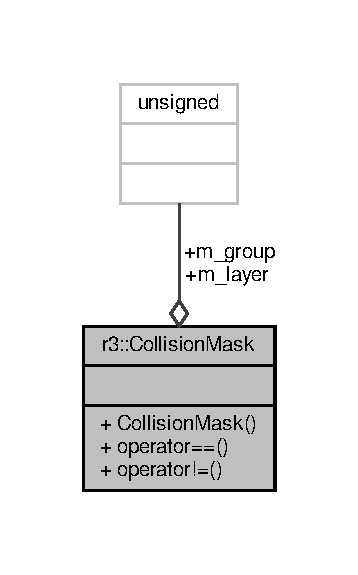
\includegraphics[width=172pt]{structr3_1_1_collision_mask__coll__graph}
\end{center}
\end{figure}
\subsection*{Public Member Functions}
\begin{DoxyCompactItemize}
\item 
\mbox{\hyperlink{structr3_1_1_collision_mask_a7f1fb1fae3d7e14677ad2590fcd661e0}{Collision\+Mask}} (unsigned int layer=0, unsigned int group=0)
\begin{DoxyCompactList}\small\item\em \mbox{\hyperlink{structr3_1_1_collision_mask}{Collision\+Mask}} constructor. \end{DoxyCompactList}\item 
bool \mbox{\hyperlink{structr3_1_1_collision_mask_a7d1315f7324fc03cee09df2c364f5c54}{operator==}} (const \mbox{\hyperlink{structr3_1_1_collision_mask}{Collision\+Mask}} \&mask) const
\item 
bool \mbox{\hyperlink{structr3_1_1_collision_mask_ae6bbe0e4390b584497c854d39ec12c6a}{operator!=}} (const \mbox{\hyperlink{structr3_1_1_collision_mask}{Collision\+Mask}} \&mask) const
\end{DoxyCompactItemize}
\subsection*{Public Attributes}
\begin{DoxyCompactItemize}
\item 
unsigned int \mbox{\hyperlink{structr3_1_1_collision_mask_a07999f53c748c86623b00e4e07d24d5f}{m\+\_\+group}}
\item 
unsigned int \mbox{\hyperlink{structr3_1_1_collision_mask_a4e3ed2227bb1782f7c6dc948a8427620}{m\+\_\+layer}}
\end{DoxyCompactItemize}


\subsection{Detailed Description}
Used to group rigid bodies. Only rigid bodies from the same layer can collide. Rigid bodies from the same group cannot collide! 

\subsection{Constructor \& Destructor Documentation}
\mbox{\Hypertarget{structr3_1_1_collision_mask_a7f1fb1fae3d7e14677ad2590fcd661e0}\label{structr3_1_1_collision_mask_a7f1fb1fae3d7e14677ad2590fcd661e0}} 
\index{r3\+::\+Collision\+Mask@{r3\+::\+Collision\+Mask}!Collision\+Mask@{Collision\+Mask}}
\index{Collision\+Mask@{Collision\+Mask}!r3\+::\+Collision\+Mask@{r3\+::\+Collision\+Mask}}
\subsubsection{\texorpdfstring{Collision\+Mask()}{CollisionMask()}}
{\footnotesize\ttfamily r3\+::\+Collision\+Mask\+::\+Collision\+Mask (\begin{DoxyParamCaption}\item[{unsigned int}]{layer = {\ttfamily 0},  }\item[{unsigned int}]{group = {\ttfamily 0} }\end{DoxyParamCaption})\hspace{0.3cm}{\ttfamily [explicit]}}



\mbox{\hyperlink{structr3_1_1_collision_mask}{Collision\+Mask}} constructor. 


\begin{DoxyParams}{Parameters}
{\em layer} & Only bodies from the same layer can collide. \\
\hline
{\em group} & Bodies from the same group can\textquotesingle{}t collide. \\
\hline
\end{DoxyParams}


\subsection{Member Function Documentation}
\mbox{\Hypertarget{structr3_1_1_collision_mask_ae6bbe0e4390b584497c854d39ec12c6a}\label{structr3_1_1_collision_mask_ae6bbe0e4390b584497c854d39ec12c6a}} 
\index{r3\+::\+Collision\+Mask@{r3\+::\+Collision\+Mask}!operator"!=@{operator"!=}}
\index{operator"!=@{operator"!=}!r3\+::\+Collision\+Mask@{r3\+::\+Collision\+Mask}}
\subsubsection{\texorpdfstring{operator"!=()}{operator!=()}}
{\footnotesize\ttfamily bool r3\+::\+Collision\+Mask\+::operator!= (\begin{DoxyParamCaption}\item[{const \mbox{\hyperlink{structr3_1_1_collision_mask}{Collision\+Mask}} \&}]{mask }\end{DoxyParamCaption}) const}

\mbox{\Hypertarget{structr3_1_1_collision_mask_a7d1315f7324fc03cee09df2c364f5c54}\label{structr3_1_1_collision_mask_a7d1315f7324fc03cee09df2c364f5c54}} 
\index{r3\+::\+Collision\+Mask@{r3\+::\+Collision\+Mask}!operator==@{operator==}}
\index{operator==@{operator==}!r3\+::\+Collision\+Mask@{r3\+::\+Collision\+Mask}}
\subsubsection{\texorpdfstring{operator==()}{operator==()}}
{\footnotesize\ttfamily bool r3\+::\+Collision\+Mask\+::operator== (\begin{DoxyParamCaption}\item[{const \mbox{\hyperlink{structr3_1_1_collision_mask}{Collision\+Mask}} \&}]{mask }\end{DoxyParamCaption}) const}



\subsection{Member Data Documentation}
\mbox{\Hypertarget{structr3_1_1_collision_mask_a07999f53c748c86623b00e4e07d24d5f}\label{structr3_1_1_collision_mask_a07999f53c748c86623b00e4e07d24d5f}} 
\index{r3\+::\+Collision\+Mask@{r3\+::\+Collision\+Mask}!m\+\_\+group@{m\+\_\+group}}
\index{m\+\_\+group@{m\+\_\+group}!r3\+::\+Collision\+Mask@{r3\+::\+Collision\+Mask}}
\subsubsection{\texorpdfstring{m\+\_\+group}{m\_group}}
{\footnotesize\ttfamily unsigned int r3\+::\+Collision\+Mask\+::m\+\_\+group}

\mbox{\Hypertarget{structr3_1_1_collision_mask_a4e3ed2227bb1782f7c6dc948a8427620}\label{structr3_1_1_collision_mask_a4e3ed2227bb1782f7c6dc948a8427620}} 
\index{r3\+::\+Collision\+Mask@{r3\+::\+Collision\+Mask}!m\+\_\+layer@{m\+\_\+layer}}
\index{m\+\_\+layer@{m\+\_\+layer}!r3\+::\+Collision\+Mask@{r3\+::\+Collision\+Mask}}
\subsubsection{\texorpdfstring{m\+\_\+layer}{m\_layer}}
{\footnotesize\ttfamily unsigned int r3\+::\+Collision\+Mask\+::m\+\_\+layer}



The documentation for this struct was generated from the following files\+:\begin{DoxyCompactItemize}
\item 
D\+:/\+Library/\+Documents/\+Job/\+Forschungsmaster/\+Projekte/\+Simulation\+Visualization/\+Rumble3\+D/\+Rumble3\+D/include/\+R3\+D/\+Rigid\+Body\+Engine/\+Collision\+Detection/\mbox{\hyperlink{_collision_mask_8h}{Collision\+Mask.\+h}}\item 
D\+:/\+Library/\+Documents/\+Job/\+Forschungsmaster/\+Projekte/\+Simulation\+Visualization/\+Rumble3\+D/\+Rumble3\+D/src/\+Rigid\+Body\+Engine/\+Collision\+Detection/\mbox{\hyperlink{_collision_mask_8cpp}{Collision\+Mask.\+cpp}}\end{DoxyCompactItemize}

\hypertarget{classr3_1_1_collision_object}{}\section{r3\+:\+:Collision\+Object Class Reference}
\label{classr3_1_1_collision_object}\index{r3\+::\+Collision\+Object@{r3\+::\+Collision\+Object}}


A \mbox{\hyperlink{classr3_1_1_collision_object}{Collision\+Object}} can collide with other collision objects in 3D space.  




{\ttfamily \#include $<$Collision\+Object.\+h$>$}



Inheritance diagram for r3\+:\+:Collision\+Object\+:\nopagebreak
\begin{figure}[H]
\begin{center}
\leavevmode
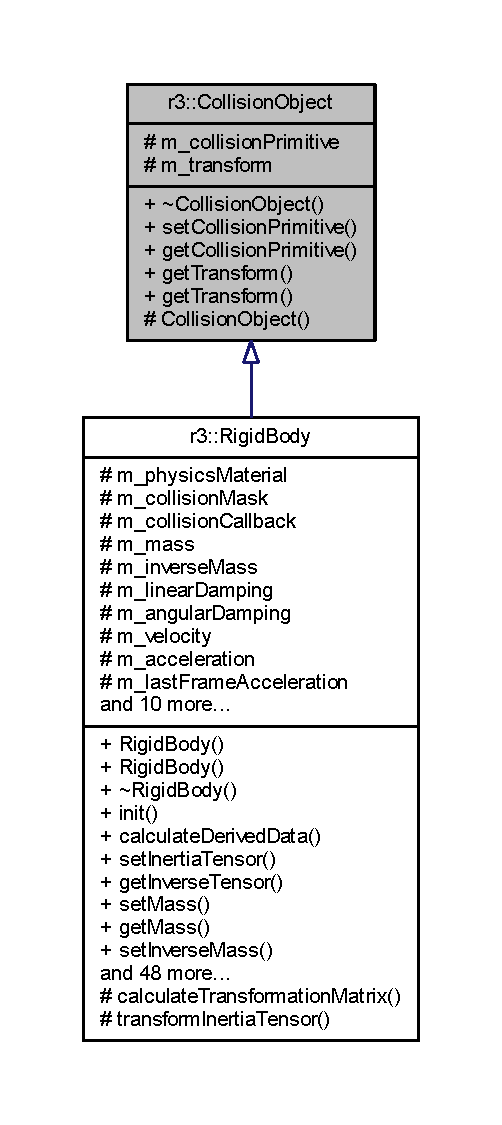
\includegraphics[width=241pt]{classr3_1_1_collision_object__inherit__graph}
\end{center}
\end{figure}


Collaboration diagram for r3\+:\+:Collision\+Object\+:\nopagebreak
\begin{figure}[H]
\begin{center}
\leavevmode
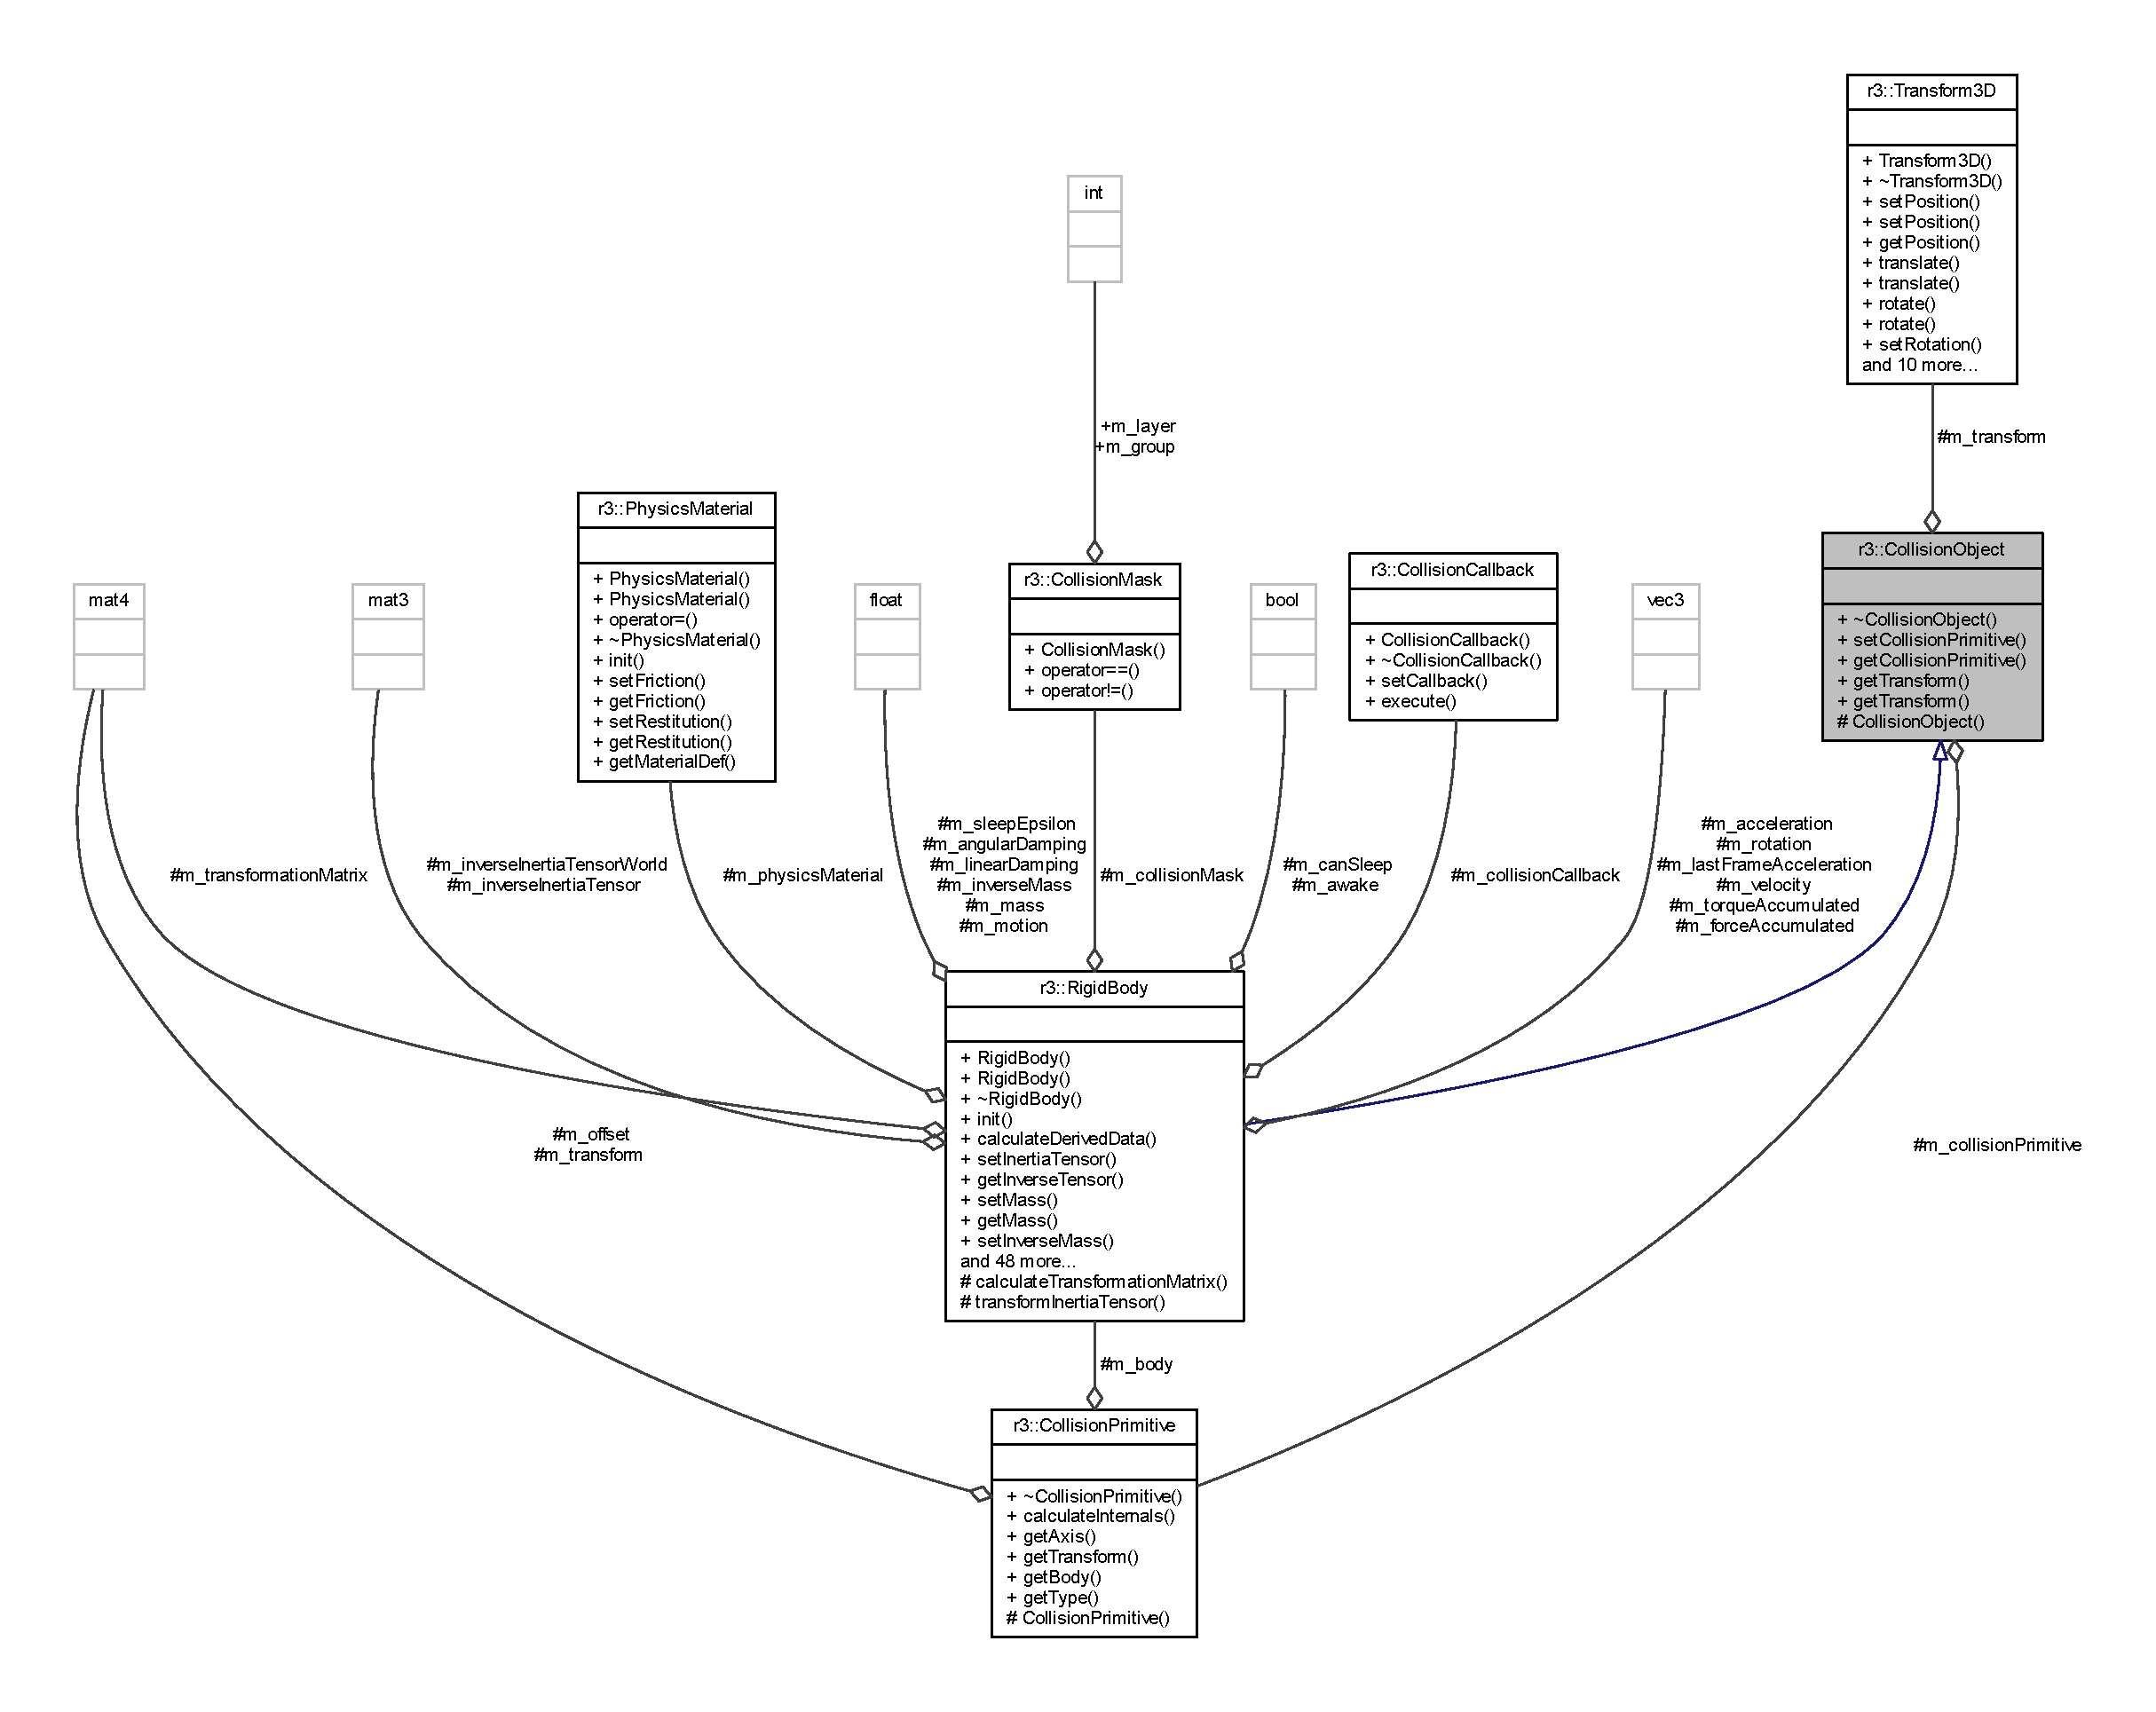
\includegraphics[width=350pt]{classr3_1_1_collision_object__coll__graph}
\end{center}
\end{figure}
\subsection*{Public Member Functions}
\begin{DoxyCompactItemize}
\item 
virtual \mbox{\hyperlink{classr3_1_1_collision_object_a26f7c8a9adb08718c98dce736cc89830}{$\sim$\+Collision\+Object}} ()
\item 
void \mbox{\hyperlink{classr3_1_1_collision_object_afaf76460298998bcbe405c0b2e6de6a6}{set\+Collision\+Primitive}} (\mbox{\hyperlink{classr3_1_1_collision_primitive}{Collision\+Primitive}} $\ast$collision\+Primitive)
\begin{DoxyCompactList}\small\item\em Set the collision primitive used for collision detection. \end{DoxyCompactList}\item 
\mbox{\hyperlink{classr3_1_1_collision_primitive}{Collision\+Primitive}} $\ast$ \mbox{\hyperlink{classr3_1_1_collision_object_aabb0d7173dacef5ffc02163557f55fa4}{get\+Collision\+Primitive}} () const
\begin{DoxyCompactList}\small\item\em Get the currently used collision primitive. \end{DoxyCompactList}\item 
const \mbox{\hyperlink{classr3_1_1_transform3_d}{Transform3D}} \& \mbox{\hyperlink{classr3_1_1_collision_object_a79e04809124cad6aeb25a66f11826fee}{get\+Transform}} () const
\begin{DoxyCompactList}\small\item\em Get the current transform. \end{DoxyCompactList}\item 
\mbox{\hyperlink{classr3_1_1_transform3_d}{Transform3D}} \& \mbox{\hyperlink{classr3_1_1_collision_object_acc41118b9a571e5aa918644aaeda6bfa}{get\+Transform}} ()
\begin{DoxyCompactList}\small\item\em Get the current transform. \end{DoxyCompactList}\end{DoxyCompactItemize}
\subsection*{Protected Member Functions}
\begin{DoxyCompactItemize}
\item 
\mbox{\hyperlink{classr3_1_1_collision_object_ad664d1dd3a03f183c46c6b7ba7327cfd}{Collision\+Object}} (\mbox{\hyperlink{classr3_1_1_collision_primitive}{Collision\+Primitive}} $\ast$collision\+Primitive=nullptr)
\begin{DoxyCompactList}\small\item\em \mbox{\hyperlink{classr3_1_1_collision_object}{Collision\+Object}} constructor. \end{DoxyCompactList}\end{DoxyCompactItemize}
\subsection*{Protected Attributes}
\begin{DoxyCompactItemize}
\item 
\mbox{\hyperlink{classr3_1_1_collision_primitive}{Collision\+Primitive}} $\ast$ \mbox{\hyperlink{classr3_1_1_collision_object_afa62ecdda20144d43f9fcf72d56642d6}{m\+\_\+collision\+Primitive}}
\item 
\mbox{\hyperlink{classr3_1_1_transform3_d}{Transform3D}} \mbox{\hyperlink{classr3_1_1_collision_object_a2ed717150a250f1b81e23ba7e5431542}{m\+\_\+transform}}
\end{DoxyCompactItemize}


\subsection{Detailed Description}
A \mbox{\hyperlink{classr3_1_1_collision_object}{Collision\+Object}} can collide with other collision objects in 3D space. 

\subsection{Constructor \& Destructor Documentation}
\mbox{\Hypertarget{classr3_1_1_collision_object_a26f7c8a9adb08718c98dce736cc89830}\label{classr3_1_1_collision_object_a26f7c8a9adb08718c98dce736cc89830}} 
\index{r3\+::\+Collision\+Object@{r3\+::\+Collision\+Object}!````~Collision\+Object@{$\sim$\+Collision\+Object}}
\index{````~Collision\+Object@{$\sim$\+Collision\+Object}!r3\+::\+Collision\+Object@{r3\+::\+Collision\+Object}}
\subsubsection{\texorpdfstring{$\sim$\+Collision\+Object()}{~CollisionObject()}}
{\footnotesize\ttfamily r3\+::\+Collision\+Object\+::$\sim$\+Collision\+Object (\begin{DoxyParamCaption}{ }\end{DoxyParamCaption})\hspace{0.3cm}{\ttfamily [virtual]}, {\ttfamily [default]}}

\mbox{\Hypertarget{classr3_1_1_collision_object_ad664d1dd3a03f183c46c6b7ba7327cfd}\label{classr3_1_1_collision_object_ad664d1dd3a03f183c46c6b7ba7327cfd}} 
\index{r3\+::\+Collision\+Object@{r3\+::\+Collision\+Object}!Collision\+Object@{Collision\+Object}}
\index{Collision\+Object@{Collision\+Object}!r3\+::\+Collision\+Object@{r3\+::\+Collision\+Object}}
\subsubsection{\texorpdfstring{Collision\+Object()}{CollisionObject()}}
{\footnotesize\ttfamily r3\+::\+Collision\+Object\+::\+Collision\+Object (\begin{DoxyParamCaption}\item[{\mbox{\hyperlink{classr3_1_1_collision_primitive}{Collision\+Primitive}} $\ast$}]{collision\+Primitive = {\ttfamily nullptr} }\end{DoxyParamCaption})\hspace{0.3cm}{\ttfamily [explicit]}, {\ttfamily [protected]}}



\mbox{\hyperlink{classr3_1_1_collision_object}{Collision\+Object}} constructor. 


\begin{DoxyParams}{Parameters}
{\em collision\+Primitive} & The initial collision primitive. \\
\hline
\end{DoxyParams}


\subsection{Member Function Documentation}
\mbox{\Hypertarget{classr3_1_1_collision_object_aabb0d7173dacef5ffc02163557f55fa4}\label{classr3_1_1_collision_object_aabb0d7173dacef5ffc02163557f55fa4}} 
\index{r3\+::\+Collision\+Object@{r3\+::\+Collision\+Object}!get\+Collision\+Primitive@{get\+Collision\+Primitive}}
\index{get\+Collision\+Primitive@{get\+Collision\+Primitive}!r3\+::\+Collision\+Object@{r3\+::\+Collision\+Object}}
\subsubsection{\texorpdfstring{get\+Collision\+Primitive()}{getCollisionPrimitive()}}
{\footnotesize\ttfamily \mbox{\hyperlink{classr3_1_1_collision_primitive}{Collision\+Primitive}} $\ast$ r3\+::\+Collision\+Object\+::get\+Collision\+Primitive (\begin{DoxyParamCaption}{ }\end{DoxyParamCaption}) const}



Get the currently used collision primitive. 

\begin{DoxyReturn}{Returns}
The collision primitive. 
\end{DoxyReturn}
\mbox{\Hypertarget{classr3_1_1_collision_object_a79e04809124cad6aeb25a66f11826fee}\label{classr3_1_1_collision_object_a79e04809124cad6aeb25a66f11826fee}} 
\index{r3\+::\+Collision\+Object@{r3\+::\+Collision\+Object}!get\+Transform@{get\+Transform}}
\index{get\+Transform@{get\+Transform}!r3\+::\+Collision\+Object@{r3\+::\+Collision\+Object}}
\subsubsection{\texorpdfstring{get\+Transform()}{getTransform()}\hspace{0.1cm}{\footnotesize\ttfamily [1/2]}}
{\footnotesize\ttfamily const \mbox{\hyperlink{classr3_1_1_transform3_d}{Transform3D}} \& r3\+::\+Collision\+Object\+::get\+Transform (\begin{DoxyParamCaption}{ }\end{DoxyParamCaption}) const}



Get the current transform. 

\begin{DoxyReturn}{Returns}
The transform. 
\end{DoxyReturn}
\mbox{\Hypertarget{classr3_1_1_collision_object_acc41118b9a571e5aa918644aaeda6bfa}\label{classr3_1_1_collision_object_acc41118b9a571e5aa918644aaeda6bfa}} 
\index{r3\+::\+Collision\+Object@{r3\+::\+Collision\+Object}!get\+Transform@{get\+Transform}}
\index{get\+Transform@{get\+Transform}!r3\+::\+Collision\+Object@{r3\+::\+Collision\+Object}}
\subsubsection{\texorpdfstring{get\+Transform()}{getTransform()}\hspace{0.1cm}{\footnotesize\ttfamily [2/2]}}
{\footnotesize\ttfamily \mbox{\hyperlink{classr3_1_1_transform3_d}{Transform3D}} \& r3\+::\+Collision\+Object\+::get\+Transform (\begin{DoxyParamCaption}{ }\end{DoxyParamCaption})}



Get the current transform. 

\begin{DoxyReturn}{Returns}
The transform. 
\end{DoxyReturn}
\mbox{\Hypertarget{classr3_1_1_collision_object_afaf76460298998bcbe405c0b2e6de6a6}\label{classr3_1_1_collision_object_afaf76460298998bcbe405c0b2e6de6a6}} 
\index{r3\+::\+Collision\+Object@{r3\+::\+Collision\+Object}!set\+Collision\+Primitive@{set\+Collision\+Primitive}}
\index{set\+Collision\+Primitive@{set\+Collision\+Primitive}!r3\+::\+Collision\+Object@{r3\+::\+Collision\+Object}}
\subsubsection{\texorpdfstring{set\+Collision\+Primitive()}{setCollisionPrimitive()}}
{\footnotesize\ttfamily void r3\+::\+Collision\+Object\+::set\+Collision\+Primitive (\begin{DoxyParamCaption}\item[{\mbox{\hyperlink{classr3_1_1_collision_primitive}{Collision\+Primitive}} $\ast$}]{collision\+Primitive }\end{DoxyParamCaption})}



Set the collision primitive used for collision detection. 


\begin{DoxyParams}{Parameters}
{\em collision\+Primitive} & The new collision primitive. \\
\hline
\end{DoxyParams}


\subsection{Member Data Documentation}
\mbox{\Hypertarget{classr3_1_1_collision_object_afa62ecdda20144d43f9fcf72d56642d6}\label{classr3_1_1_collision_object_afa62ecdda20144d43f9fcf72d56642d6}} 
\index{r3\+::\+Collision\+Object@{r3\+::\+Collision\+Object}!m\+\_\+collision\+Primitive@{m\+\_\+collision\+Primitive}}
\index{m\+\_\+collision\+Primitive@{m\+\_\+collision\+Primitive}!r3\+::\+Collision\+Object@{r3\+::\+Collision\+Object}}
\subsubsection{\texorpdfstring{m\+\_\+collision\+Primitive}{m\_collisionPrimitive}}
{\footnotesize\ttfamily \mbox{\hyperlink{classr3_1_1_collision_primitive}{Collision\+Primitive}}$\ast$ r3\+::\+Collision\+Object\+::m\+\_\+collision\+Primitive\hspace{0.3cm}{\ttfamily [protected]}}

\mbox{\Hypertarget{classr3_1_1_collision_object_a2ed717150a250f1b81e23ba7e5431542}\label{classr3_1_1_collision_object_a2ed717150a250f1b81e23ba7e5431542}} 
\index{r3\+::\+Collision\+Object@{r3\+::\+Collision\+Object}!m\+\_\+transform@{m\+\_\+transform}}
\index{m\+\_\+transform@{m\+\_\+transform}!r3\+::\+Collision\+Object@{r3\+::\+Collision\+Object}}
\subsubsection{\texorpdfstring{m\+\_\+transform}{m\_transform}}
{\footnotesize\ttfamily \mbox{\hyperlink{classr3_1_1_transform3_d}{Transform3D}} r3\+::\+Collision\+Object\+::m\+\_\+transform\hspace{0.3cm}{\ttfamily [protected]}}



The documentation for this class was generated from the following files\+:\begin{DoxyCompactItemize}
\item 
D\+:/\+Library/\+Documents/\+Job/\+Forschungsmaster/\+Projekte/\+Simulation\+Visualization/\+Rumble3\+D/\+Rumble3\+D/include/\+R3\+D/\+Rigid\+Body\+Engine/\mbox{\hyperlink{_collision_object_8h}{Collision\+Object.\+h}}\item 
D\+:/\+Library/\+Documents/\+Job/\+Forschungsmaster/\+Projekte/\+Simulation\+Visualization/\+Rumble3\+D/\+Rumble3\+D/src/\+Rigid\+Body\+Engine/\mbox{\hyperlink{_collision_object_8cpp}{Collision\+Object.\+cpp}}\end{DoxyCompactItemize}

\hypertarget{classr3_1_1_collision_pair}{}\doxysection{r3\+::Collision\+Pair Class Reference}
\label{classr3_1_1_collision_pair}\index{r3::CollisionPair@{r3::CollisionPair}}


A \mbox{\hyperlink{classr3_1_1_collision_pair}{Collision\+Pair}} describes a potential collision between two rigid bodies.  




{\ttfamily \#include $<$Collision\+Pair.\+h$>$}



Collaboration diagram for r3\+::Collision\+Pair\+:\nopagebreak
\begin{figure}[H]
\begin{center}
\leavevmode
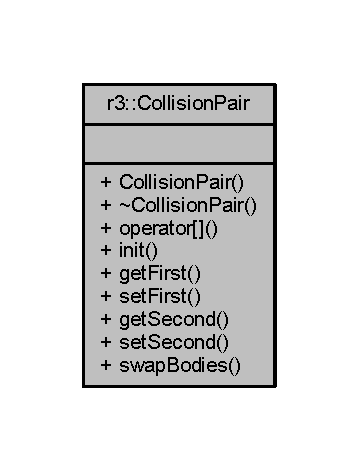
\includegraphics[width=170pt]{classr3_1_1_collision_pair__coll__graph}
\end{center}
\end{figure}
\doxysubsection*{Public Member Functions}
\begin{DoxyCompactItemize}
\item 
\mbox{\hyperlink{classr3_1_1_collision_pair_ab6434bde3aa02c2655e26a976570db01}{Collision\+Pair}} (\mbox{\hyperlink{classr3_1_1_rigid_body}{Rigid\+Body}} $\ast$first=nullptr, \mbox{\hyperlink{classr3_1_1_rigid_body}{Rigid\+Body}} $\ast$second=nullptr)
\begin{DoxyCompactList}\small\item\em \mbox{\hyperlink{classr3_1_1_collision_pair}{Collision\+Pair}} constructor. \end{DoxyCompactList}\item 
\mbox{\hyperlink{classr3_1_1_collision_pair_a38ae2cf6732b5a1b4dfdc544bbff82e0}{$\sim$\+Collision\+Pair}} ()
\item 
\mbox{\hyperlink{classr3_1_1_rigid_body}{Rigid\+Body}} $\ast$ \mbox{\hyperlink{classr3_1_1_collision_pair_a8d56c936cb56821247c5b1a684578c0a}{operator\mbox{[}$\,$\mbox{]}}} (int index) const
\begin{DoxyCompactList}\small\item\em Get a rigid body by index. \end{DoxyCompactList}\item 
void \mbox{\hyperlink{classr3_1_1_collision_pair_a7e64e731162cfdc3222d8f02b7c886b1}{init}} (\mbox{\hyperlink{classr3_1_1_rigid_body}{Rigid\+Body}} $\ast$first, \mbox{\hyperlink{classr3_1_1_rigid_body}{Rigid\+Body}} $\ast$second)
\begin{DoxyCompactList}\small\item\em Initialize the pair with two potentially colliding rigid bodies. \end{DoxyCompactList}\item 
\mbox{\hyperlink{classr3_1_1_rigid_body}{Rigid\+Body}} $\ast$ \mbox{\hyperlink{classr3_1_1_collision_pair_a603f9437f7fa4aa5253ad26247ee75ae}{get\+First}} () const
\begin{DoxyCompactList}\small\item\em Get the first rigid body. \end{DoxyCompactList}\item 
void \mbox{\hyperlink{classr3_1_1_collision_pair_ac900e6382810b6820dc3f4ecf832bb6b}{set\+First}} (\mbox{\hyperlink{classr3_1_1_rigid_body}{Rigid\+Body}} $\ast$first)
\begin{DoxyCompactList}\small\item\em Set the first rigid body. \end{DoxyCompactList}\item 
\mbox{\hyperlink{classr3_1_1_rigid_body}{Rigid\+Body}} $\ast$ \mbox{\hyperlink{classr3_1_1_collision_pair_a218a4ee7500ed53c3ba5384833afff5a}{get\+Second}} () const
\begin{DoxyCompactList}\small\item\em Get the second rigid body. \end{DoxyCompactList}\item 
void \mbox{\hyperlink{classr3_1_1_collision_pair_acb8c2f4a2c44eeffb8a3d76023db985b}{set\+Second}} (\mbox{\hyperlink{classr3_1_1_rigid_body}{Rigid\+Body}} $\ast$second)
\begin{DoxyCompactList}\small\item\em Set the second rigid body. \end{DoxyCompactList}\item 
void \mbox{\hyperlink{classr3_1_1_collision_pair_a8ef5b5bae7be7db3ed2574ecd9e5bf9a}{swap\+Bodies}} ()
\begin{DoxyCompactList}\small\item\em Swap first and second rigid body. \end{DoxyCompactList}\end{DoxyCompactItemize}


\doxysubsection{Detailed Description}
A \mbox{\hyperlink{classr3_1_1_collision_pair}{Collision\+Pair}} describes a potential collision between two rigid bodies. 

\doxysubsection{Constructor \& Destructor Documentation}
\mbox{\Hypertarget{classr3_1_1_collision_pair_ab6434bde3aa02c2655e26a976570db01}\label{classr3_1_1_collision_pair_ab6434bde3aa02c2655e26a976570db01}} 
\index{r3::CollisionPair@{r3::CollisionPair}!CollisionPair@{CollisionPair}}
\index{CollisionPair@{CollisionPair}!r3::CollisionPair@{r3::CollisionPair}}
\doxysubsubsection{\texorpdfstring{CollisionPair()}{CollisionPair()}}
{\footnotesize\ttfamily r3\+::\+Collision\+Pair\+::\+Collision\+Pair (\begin{DoxyParamCaption}\item[{\mbox{\hyperlink{classr3_1_1_rigid_body}{Rigid\+Body}} $\ast$}]{first = {\ttfamily nullptr},  }\item[{\mbox{\hyperlink{classr3_1_1_rigid_body}{Rigid\+Body}} $\ast$}]{second = {\ttfamily nullptr} }\end{DoxyParamCaption})\hspace{0.3cm}{\ttfamily [explicit]}}



\mbox{\hyperlink{classr3_1_1_collision_pair}{Collision\+Pair}} constructor. 


\begin{DoxyParams}{Parameters}
{\em first} & First rigid body \\
\hline
{\em second} & Second rigid body \\
\hline
\end{DoxyParams}
\mbox{\Hypertarget{classr3_1_1_collision_pair_a38ae2cf6732b5a1b4dfdc544bbff82e0}\label{classr3_1_1_collision_pair_a38ae2cf6732b5a1b4dfdc544bbff82e0}} 
\index{r3::CollisionPair@{r3::CollisionPair}!````~CollisionPair@{$\sim$CollisionPair}}
\index{````~CollisionPair@{$\sim$CollisionPair}!r3::CollisionPair@{r3::CollisionPair}}
\doxysubsubsection{\texorpdfstring{$\sim$CollisionPair()}{~CollisionPair()}}
{\footnotesize\ttfamily r3\+::\+Collision\+Pair\+::$\sim$\+Collision\+Pair (\begin{DoxyParamCaption}{ }\end{DoxyParamCaption})\hspace{0.3cm}{\ttfamily [default]}}



\doxysubsection{Member Function Documentation}
\mbox{\Hypertarget{classr3_1_1_collision_pair_a603f9437f7fa4aa5253ad26247ee75ae}\label{classr3_1_1_collision_pair_a603f9437f7fa4aa5253ad26247ee75ae}} 
\index{r3::CollisionPair@{r3::CollisionPair}!getFirst@{getFirst}}
\index{getFirst@{getFirst}!r3::CollisionPair@{r3::CollisionPair}}
\doxysubsubsection{\texorpdfstring{getFirst()}{getFirst()}}
{\footnotesize\ttfamily \mbox{\hyperlink{classr3_1_1_rigid_body}{Rigid\+Body}} $\ast$ r3\+::\+Collision\+Pair\+::get\+First (\begin{DoxyParamCaption}{ }\end{DoxyParamCaption}) const}



Get the first rigid body. 

\begin{DoxyReturn}{Returns}
The first rigid body 
\end{DoxyReturn}
\mbox{\Hypertarget{classr3_1_1_collision_pair_a218a4ee7500ed53c3ba5384833afff5a}\label{classr3_1_1_collision_pair_a218a4ee7500ed53c3ba5384833afff5a}} 
\index{r3::CollisionPair@{r3::CollisionPair}!getSecond@{getSecond}}
\index{getSecond@{getSecond}!r3::CollisionPair@{r3::CollisionPair}}
\doxysubsubsection{\texorpdfstring{getSecond()}{getSecond()}}
{\footnotesize\ttfamily \mbox{\hyperlink{classr3_1_1_rigid_body}{Rigid\+Body}} $\ast$ r3\+::\+Collision\+Pair\+::get\+Second (\begin{DoxyParamCaption}{ }\end{DoxyParamCaption}) const}



Get the second rigid body. 

\begin{DoxyReturn}{Returns}
The second rigid body 
\end{DoxyReturn}
\mbox{\Hypertarget{classr3_1_1_collision_pair_a7e64e731162cfdc3222d8f02b7c886b1}\label{classr3_1_1_collision_pair_a7e64e731162cfdc3222d8f02b7c886b1}} 
\index{r3::CollisionPair@{r3::CollisionPair}!init@{init}}
\index{init@{init}!r3::CollisionPair@{r3::CollisionPair}}
\doxysubsubsection{\texorpdfstring{init()}{init()}}
{\footnotesize\ttfamily void r3\+::\+Collision\+Pair\+::init (\begin{DoxyParamCaption}\item[{\mbox{\hyperlink{classr3_1_1_rigid_body}{Rigid\+Body}} $\ast$}]{first,  }\item[{\mbox{\hyperlink{classr3_1_1_rigid_body}{Rigid\+Body}} $\ast$}]{second }\end{DoxyParamCaption})}



Initialize the pair with two potentially colliding rigid bodies. 


\begin{DoxyParams}{Parameters}
{\em first} & The first rigid body \\
\hline
{\em second} & The second rigid body \\
\hline
\end{DoxyParams}
\mbox{\Hypertarget{classr3_1_1_collision_pair_a8d56c936cb56821247c5b1a684578c0a}\label{classr3_1_1_collision_pair_a8d56c936cb56821247c5b1a684578c0a}} 
\index{r3::CollisionPair@{r3::CollisionPair}!operator\mbox{[}\mbox{]}@{operator[]}}
\index{operator\mbox{[}\mbox{]}@{operator[]}!r3::CollisionPair@{r3::CollisionPair}}
\doxysubsubsection{\texorpdfstring{operator[]()}{operator[]()}}
{\footnotesize\ttfamily \mbox{\hyperlink{classr3_1_1_rigid_body}{Rigid\+Body}} $\ast$ r3\+::\+Collision\+Pair\+::operator\mbox{[}$\,$\mbox{]} (\begin{DoxyParamCaption}\item[{int}]{index }\end{DoxyParamCaption}) const}



Get a rigid body by index. 


\begin{DoxyParams}{Parameters}
{\em index} & Either 0 (first body) or 1 (second body) \\
\hline
\end{DoxyParams}
\begin{DoxyReturn}{Returns}
First or second rigid body. 
\end{DoxyReturn}
\mbox{\Hypertarget{classr3_1_1_collision_pair_ac900e6382810b6820dc3f4ecf832bb6b}\label{classr3_1_1_collision_pair_ac900e6382810b6820dc3f4ecf832bb6b}} 
\index{r3::CollisionPair@{r3::CollisionPair}!setFirst@{setFirst}}
\index{setFirst@{setFirst}!r3::CollisionPair@{r3::CollisionPair}}
\doxysubsubsection{\texorpdfstring{setFirst()}{setFirst()}}
{\footnotesize\ttfamily void r3\+::\+Collision\+Pair\+::set\+First (\begin{DoxyParamCaption}\item[{\mbox{\hyperlink{classr3_1_1_rigid_body}{Rigid\+Body}} $\ast$}]{first }\end{DoxyParamCaption})}



Set the first rigid body. 


\begin{DoxyParams}{Parameters}
{\em first} & A rigid body, which might collide with the second one. \\
\hline
\end{DoxyParams}
\mbox{\Hypertarget{classr3_1_1_collision_pair_acb8c2f4a2c44eeffb8a3d76023db985b}\label{classr3_1_1_collision_pair_acb8c2f4a2c44eeffb8a3d76023db985b}} 
\index{r3::CollisionPair@{r3::CollisionPair}!setSecond@{setSecond}}
\index{setSecond@{setSecond}!r3::CollisionPair@{r3::CollisionPair}}
\doxysubsubsection{\texorpdfstring{setSecond()}{setSecond()}}
{\footnotesize\ttfamily void r3\+::\+Collision\+Pair\+::set\+Second (\begin{DoxyParamCaption}\item[{\mbox{\hyperlink{classr3_1_1_rigid_body}{Rigid\+Body}} $\ast$}]{second }\end{DoxyParamCaption})}



Set the second rigid body. 


\begin{DoxyParams}{Parameters}
{\em second} & A rigid body, which might collide with the first one. \\
\hline
\end{DoxyParams}
\mbox{\Hypertarget{classr3_1_1_collision_pair_a8ef5b5bae7be7db3ed2574ecd9e5bf9a}\label{classr3_1_1_collision_pair_a8ef5b5bae7be7db3ed2574ecd9e5bf9a}} 
\index{r3::CollisionPair@{r3::CollisionPair}!swapBodies@{swapBodies}}
\index{swapBodies@{swapBodies}!r3::CollisionPair@{r3::CollisionPair}}
\doxysubsubsection{\texorpdfstring{swapBodies()}{swapBodies()}}
{\footnotesize\ttfamily void r3\+::\+Collision\+Pair\+::swap\+Bodies (\begin{DoxyParamCaption}{ }\end{DoxyParamCaption})}



Swap first and second rigid body. 



The documentation for this class was generated from the following files\+:\begin{DoxyCompactItemize}
\item 
/home/nelaty/\+Development/\+Repositories/\+Rumble3\+D/include/\+R3\+D/\+Rigid\+Body\+Engine/\+Collision\+Detection/\mbox{\hyperlink{_collision_pair_8h}{Collision\+Pair.\+h}}\item 
/home/nelaty/\+Development/\+Repositories/\+Rumble3\+D/src/\+Rigid\+Body\+Engine/\+Collision\+Detection/\mbox{\hyperlink{_collision_pair_8cpp}{Collision\+Pair.\+cpp}}\end{DoxyCompactItemize}

\hypertarget{classr3_1_1_collision_plane}{}\section{r3\+:\+:Collision\+Plane Class Reference}
\label{classr3_1_1_collision_plane}\index{r3\+::\+Collision\+Plane@{r3\+::\+Collision\+Plane}}


\mbox{\hyperlink{classr3_1_1_collision_primitive}{Collision\+Primitive}} that represents a plane.  




{\ttfamily \#include $<$Collision\+Plane.\+h$>$}



Inheritance diagram for r3\+:\+:Collision\+Plane\+:\nopagebreak
\begin{figure}[H]
\begin{center}
\leavevmode
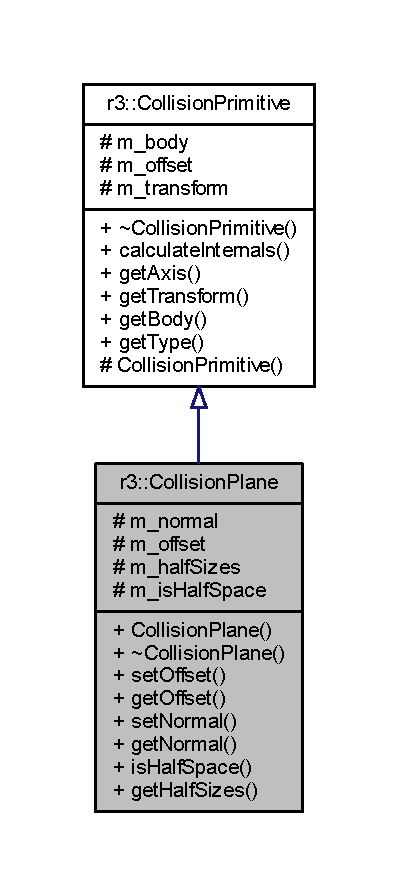
\includegraphics[width=191pt]{classr3_1_1_collision_plane__inherit__graph}
\end{center}
\end{figure}


Collaboration diagram for r3\+:\+:Collision\+Plane\+:\nopagebreak
\begin{figure}[H]
\begin{center}
\leavevmode
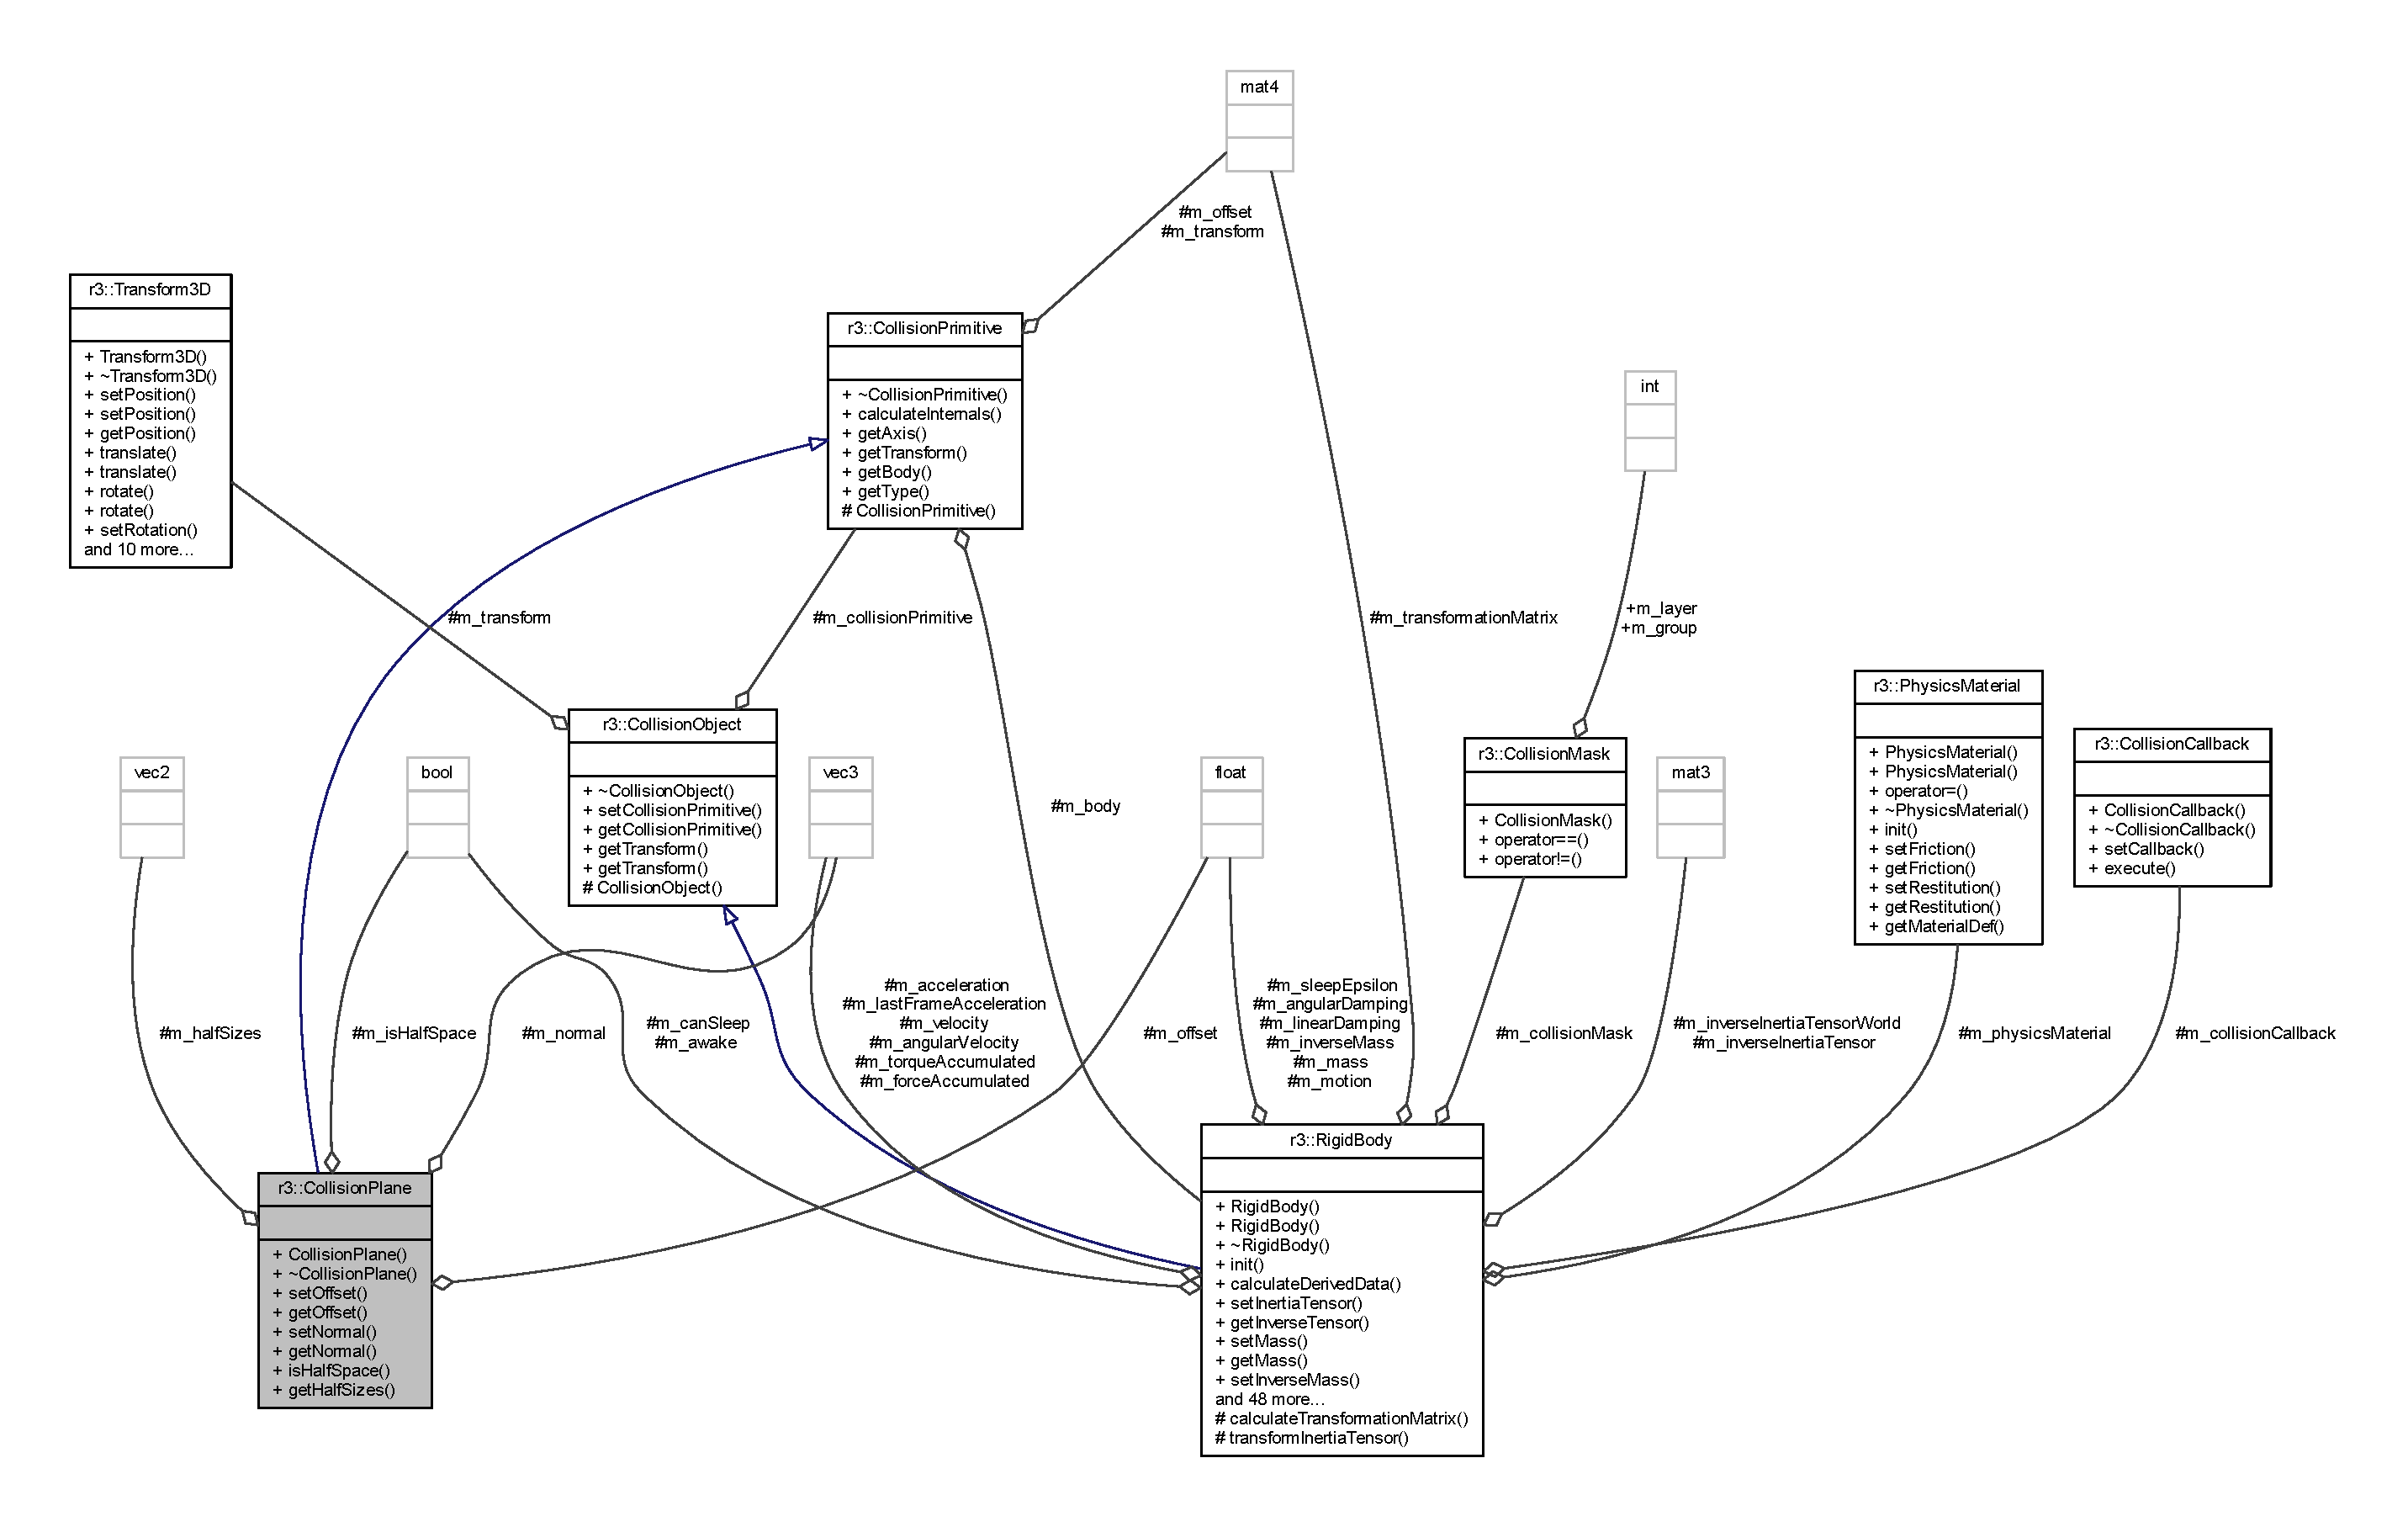
\includegraphics[width=350pt]{classr3_1_1_collision_plane__coll__graph}
\end{center}
\end{figure}
\subsection*{Public Member Functions}
\begin{DoxyCompactItemize}
\item 
\mbox{\hyperlink{classr3_1_1_collision_plane_ae3f8642b62667018e4a4c3120880fd0f}{Collision\+Plane}} (const glm\+::vec3 \&normal, \mbox{\hyperlink{namespacer3_ab2016b3e3f743fb735afce242f0dc1eb}{real}} offset, const glm\+::vec2 \&half\+Sizes=glm\+::vec2(1.\+0f, 1.\+0f), bool is\+Half\+Space=false)
\begin{DoxyCompactList}\small\item\em \mbox{\hyperlink{classr3_1_1_collision_plane}{Collision\+Plane}} constructor. \end{DoxyCompactList}\item 
\mbox{\hyperlink{classr3_1_1_collision_plane_a4c83b51c544a5fda9d949baced5cea02}{$\sim$\+Collision\+Plane}} ()
\item 
void \mbox{\hyperlink{classr3_1_1_collision_plane_ae37e09e6b807cdd800671daa5623b073}{set\+Offset}} (\mbox{\hyperlink{namespacer3_ab2016b3e3f743fb735afce242f0dc1eb}{real}} offset)
\begin{DoxyCompactList}\small\item\em Set the current offset. \end{DoxyCompactList}\item 
\mbox{\hyperlink{namespacer3_ab2016b3e3f743fb735afce242f0dc1eb}{real}} \mbox{\hyperlink{classr3_1_1_collision_plane_a62e2b4bd6a811f8d2541329cd9a49bf8}{get\+Offset}} () const
\begin{DoxyCompactList}\small\item\em Get the current offset. \end{DoxyCompactList}\item 
void \mbox{\hyperlink{classr3_1_1_collision_plane_a1fa140b6648f14bef9720ac0d4eefc99}{set\+Normal}} (const glm\+::vec3 \&normal)
\begin{DoxyCompactList}\small\item\em Set the current normal. \end{DoxyCompactList}\item 
glm\+::vec3 \mbox{\hyperlink{classr3_1_1_collision_plane_aa6605acf447da4e45084e6d25c1067ad}{get\+Normal}} () const
\begin{DoxyCompactList}\small\item\em Get the current normal. \end{DoxyCompactList}\item 
bool \mbox{\hyperlink{classr3_1_1_collision_plane_a87f5071d181b4c643b42cb2448464be2}{is\+Half\+Space}} () const
\begin{DoxyCompactList}\small\item\em Check if this plane defines a half space. \end{DoxyCompactList}\item 
const glm\+::vec2 \& \mbox{\hyperlink{classr3_1_1_collision_plane_ab48030fbf5bc17cd5ad81e5eb654a4b4}{get\+Half\+Sizes}} () const
\begin{DoxyCompactList}\small\item\em Get the size of the plane. \end{DoxyCompactList}\end{DoxyCompactItemize}
\subsection*{Protected Attributes}
\begin{DoxyCompactItemize}
\item 
glm\+::vec3 \mbox{\hyperlink{classr3_1_1_collision_plane_ab65e832434d2da433e79c93ac12f4b43}{m\+\_\+normal}}
\item 
\mbox{\hyperlink{namespacer3_ab2016b3e3f743fb735afce242f0dc1eb}{real}} \mbox{\hyperlink{classr3_1_1_collision_plane_a8ae3c28197b05088e405ff9944632f74}{m\+\_\+offset}}
\item 
glm\+::vec2 \mbox{\hyperlink{classr3_1_1_collision_plane_a8e642d9075ceebd029f3869ace65dd5f}{m\+\_\+half\+Sizes}}
\item 
bool \mbox{\hyperlink{classr3_1_1_collision_plane_a6d560c5f7627efec1d094905ec4e7d60}{m\+\_\+is\+Half\+Space}}
\end{DoxyCompactItemize}
\subsection*{Additional Inherited Members}


\subsection{Detailed Description}
\mbox{\hyperlink{classr3_1_1_collision_primitive}{Collision\+Primitive}} that represents a plane. 

\subsection{Constructor \& Destructor Documentation}
\mbox{\Hypertarget{classr3_1_1_collision_plane_ae3f8642b62667018e4a4c3120880fd0f}\label{classr3_1_1_collision_plane_ae3f8642b62667018e4a4c3120880fd0f}} 
\index{r3\+::\+Collision\+Plane@{r3\+::\+Collision\+Plane}!Collision\+Plane@{Collision\+Plane}}
\index{Collision\+Plane@{Collision\+Plane}!r3\+::\+Collision\+Plane@{r3\+::\+Collision\+Plane}}
\subsubsection{\texorpdfstring{Collision\+Plane()}{CollisionPlane()}}
{\footnotesize\ttfamily r3\+::\+Collision\+Plane\+::\+Collision\+Plane (\begin{DoxyParamCaption}\item[{const glm\+::vec3 \&}]{normal,  }\item[{\mbox{\hyperlink{namespacer3_ab2016b3e3f743fb735afce242f0dc1eb}{real}}}]{offset,  }\item[{const glm\+::vec2 \&}]{half\+Sizes = {\ttfamily glm\+:\+:vec2(1.0f,~1.0f)},  }\item[{bool}]{is\+Half\+Space = {\ttfamily false} }\end{DoxyParamCaption})}



\mbox{\hyperlink{classr3_1_1_collision_plane}{Collision\+Plane}} constructor. 


\begin{DoxyParams}{Parameters}
{\em normal} & Defines the front side of the plane. \\
\hline
{\em offset} & The offset along the normal. \\
\hline
{\em half\+Sizes} & Size of the plane. \\
\hline
{\em is\+Half\+Space} & Flag to also use a plane as a half space. \\
\hline
\end{DoxyParams}
\mbox{\Hypertarget{classr3_1_1_collision_plane_a4c83b51c544a5fda9d949baced5cea02}\label{classr3_1_1_collision_plane_a4c83b51c544a5fda9d949baced5cea02}} 
\index{r3\+::\+Collision\+Plane@{r3\+::\+Collision\+Plane}!````~Collision\+Plane@{$\sim$\+Collision\+Plane}}
\index{````~Collision\+Plane@{$\sim$\+Collision\+Plane}!r3\+::\+Collision\+Plane@{r3\+::\+Collision\+Plane}}
\subsubsection{\texorpdfstring{$\sim$\+Collision\+Plane()}{~CollisionPlane()}}
{\footnotesize\ttfamily r3\+::\+Collision\+Plane\+::$\sim$\+Collision\+Plane (\begin{DoxyParamCaption}{ }\end{DoxyParamCaption})\hspace{0.3cm}{\ttfamily [default]}}



\subsection{Member Function Documentation}
\mbox{\Hypertarget{classr3_1_1_collision_plane_ab48030fbf5bc17cd5ad81e5eb654a4b4}\label{classr3_1_1_collision_plane_ab48030fbf5bc17cd5ad81e5eb654a4b4}} 
\index{r3\+::\+Collision\+Plane@{r3\+::\+Collision\+Plane}!get\+Half\+Sizes@{get\+Half\+Sizes}}
\index{get\+Half\+Sizes@{get\+Half\+Sizes}!r3\+::\+Collision\+Plane@{r3\+::\+Collision\+Plane}}
\subsubsection{\texorpdfstring{get\+Half\+Sizes()}{getHalfSizes()}}
{\footnotesize\ttfamily const glm\+::vec2 \& r3\+::\+Collision\+Plane\+::get\+Half\+Sizes (\begin{DoxyParamCaption}{ }\end{DoxyParamCaption}) const}



Get the size of the plane. 

\begin{DoxyReturn}{Returns}
The half sizes. 
\end{DoxyReturn}
\mbox{\Hypertarget{classr3_1_1_collision_plane_aa6605acf447da4e45084e6d25c1067ad}\label{classr3_1_1_collision_plane_aa6605acf447da4e45084e6d25c1067ad}} 
\index{r3\+::\+Collision\+Plane@{r3\+::\+Collision\+Plane}!get\+Normal@{get\+Normal}}
\index{get\+Normal@{get\+Normal}!r3\+::\+Collision\+Plane@{r3\+::\+Collision\+Plane}}
\subsubsection{\texorpdfstring{get\+Normal()}{getNormal()}}
{\footnotesize\ttfamily glm\+::vec3 r3\+::\+Collision\+Plane\+::get\+Normal (\begin{DoxyParamCaption}{ }\end{DoxyParamCaption}) const}



Get the current normal. 

\begin{DoxyReturn}{Returns}
The normal. 
\end{DoxyReturn}
\mbox{\Hypertarget{classr3_1_1_collision_plane_a62e2b4bd6a811f8d2541329cd9a49bf8}\label{classr3_1_1_collision_plane_a62e2b4bd6a811f8d2541329cd9a49bf8}} 
\index{r3\+::\+Collision\+Plane@{r3\+::\+Collision\+Plane}!get\+Offset@{get\+Offset}}
\index{get\+Offset@{get\+Offset}!r3\+::\+Collision\+Plane@{r3\+::\+Collision\+Plane}}
\subsubsection{\texorpdfstring{get\+Offset()}{getOffset()}}
{\footnotesize\ttfamily \mbox{\hyperlink{namespacer3_ab2016b3e3f743fb735afce242f0dc1eb}{real}} r3\+::\+Collision\+Plane\+::get\+Offset (\begin{DoxyParamCaption}{ }\end{DoxyParamCaption}) const}



Get the current offset. 

\begin{DoxyReturn}{Returns}
The offset along the normal 
\end{DoxyReturn}
\mbox{\Hypertarget{classr3_1_1_collision_plane_a87f5071d181b4c643b42cb2448464be2}\label{classr3_1_1_collision_plane_a87f5071d181b4c643b42cb2448464be2}} 
\index{r3\+::\+Collision\+Plane@{r3\+::\+Collision\+Plane}!is\+Half\+Space@{is\+Half\+Space}}
\index{is\+Half\+Space@{is\+Half\+Space}!r3\+::\+Collision\+Plane@{r3\+::\+Collision\+Plane}}
\subsubsection{\texorpdfstring{is\+Half\+Space()}{isHalfSpace()}}
{\footnotesize\ttfamily bool r3\+::\+Collision\+Plane\+::is\+Half\+Space (\begin{DoxyParamCaption}{ }\end{DoxyParamCaption}) const}



Check if this plane defines a half space. 

\begin{DoxyReturn}{Returns}
True if it is a half space, false otherwise. 
\end{DoxyReturn}
\mbox{\Hypertarget{classr3_1_1_collision_plane_a1fa140b6648f14bef9720ac0d4eefc99}\label{classr3_1_1_collision_plane_a1fa140b6648f14bef9720ac0d4eefc99}} 
\index{r3\+::\+Collision\+Plane@{r3\+::\+Collision\+Plane}!set\+Normal@{set\+Normal}}
\index{set\+Normal@{set\+Normal}!r3\+::\+Collision\+Plane@{r3\+::\+Collision\+Plane}}
\subsubsection{\texorpdfstring{set\+Normal()}{setNormal()}}
{\footnotesize\ttfamily void r3\+::\+Collision\+Plane\+::set\+Normal (\begin{DoxyParamCaption}\item[{const glm\+::vec3 \&}]{normal }\end{DoxyParamCaption})}



Set the current normal. 


\begin{DoxyParams}{Parameters}
{\em normal} & The new normal. \\
\hline
\end{DoxyParams}
\mbox{\Hypertarget{classr3_1_1_collision_plane_ae37e09e6b807cdd800671daa5623b073}\label{classr3_1_1_collision_plane_ae37e09e6b807cdd800671daa5623b073}} 
\index{r3\+::\+Collision\+Plane@{r3\+::\+Collision\+Plane}!set\+Offset@{set\+Offset}}
\index{set\+Offset@{set\+Offset}!r3\+::\+Collision\+Plane@{r3\+::\+Collision\+Plane}}
\subsubsection{\texorpdfstring{set\+Offset()}{setOffset()}}
{\footnotesize\ttfamily void r3\+::\+Collision\+Plane\+::set\+Offset (\begin{DoxyParamCaption}\item[{\mbox{\hyperlink{namespacer3_ab2016b3e3f743fb735afce242f0dc1eb}{real}}}]{offset }\end{DoxyParamCaption})}



Set the current offset. 


\begin{DoxyParams}{Parameters}
{\em offset} & The offset along the normal. \\
\hline
\end{DoxyParams}


\subsection{Member Data Documentation}
\mbox{\Hypertarget{classr3_1_1_collision_plane_a8e642d9075ceebd029f3869ace65dd5f}\label{classr3_1_1_collision_plane_a8e642d9075ceebd029f3869ace65dd5f}} 
\index{r3\+::\+Collision\+Plane@{r3\+::\+Collision\+Plane}!m\+\_\+half\+Sizes@{m\+\_\+half\+Sizes}}
\index{m\+\_\+half\+Sizes@{m\+\_\+half\+Sizes}!r3\+::\+Collision\+Plane@{r3\+::\+Collision\+Plane}}
\subsubsection{\texorpdfstring{m\+\_\+half\+Sizes}{m\_halfSizes}}
{\footnotesize\ttfamily glm\+::vec2 r3\+::\+Collision\+Plane\+::m\+\_\+half\+Sizes\hspace{0.3cm}{\ttfamily [protected]}}

\mbox{\Hypertarget{classr3_1_1_collision_plane_a6d560c5f7627efec1d094905ec4e7d60}\label{classr3_1_1_collision_plane_a6d560c5f7627efec1d094905ec4e7d60}} 
\index{r3\+::\+Collision\+Plane@{r3\+::\+Collision\+Plane}!m\+\_\+is\+Half\+Space@{m\+\_\+is\+Half\+Space}}
\index{m\+\_\+is\+Half\+Space@{m\+\_\+is\+Half\+Space}!r3\+::\+Collision\+Plane@{r3\+::\+Collision\+Plane}}
\subsubsection{\texorpdfstring{m\+\_\+is\+Half\+Space}{m\_isHalfSpace}}
{\footnotesize\ttfamily bool r3\+::\+Collision\+Plane\+::m\+\_\+is\+Half\+Space\hspace{0.3cm}{\ttfamily [protected]}}

\mbox{\Hypertarget{classr3_1_1_collision_plane_ab65e832434d2da433e79c93ac12f4b43}\label{classr3_1_1_collision_plane_ab65e832434d2da433e79c93ac12f4b43}} 
\index{r3\+::\+Collision\+Plane@{r3\+::\+Collision\+Plane}!m\+\_\+normal@{m\+\_\+normal}}
\index{m\+\_\+normal@{m\+\_\+normal}!r3\+::\+Collision\+Plane@{r3\+::\+Collision\+Plane}}
\subsubsection{\texorpdfstring{m\+\_\+normal}{m\_normal}}
{\footnotesize\ttfamily glm\+::vec3 r3\+::\+Collision\+Plane\+::m\+\_\+normal\hspace{0.3cm}{\ttfamily [protected]}}

\mbox{\Hypertarget{classr3_1_1_collision_plane_a8ae3c28197b05088e405ff9944632f74}\label{classr3_1_1_collision_plane_a8ae3c28197b05088e405ff9944632f74}} 
\index{r3\+::\+Collision\+Plane@{r3\+::\+Collision\+Plane}!m\+\_\+offset@{m\+\_\+offset}}
\index{m\+\_\+offset@{m\+\_\+offset}!r3\+::\+Collision\+Plane@{r3\+::\+Collision\+Plane}}
\subsubsection{\texorpdfstring{m\+\_\+offset}{m\_offset}}
{\footnotesize\ttfamily \mbox{\hyperlink{namespacer3_ab2016b3e3f743fb735afce242f0dc1eb}{real}} r3\+::\+Collision\+Plane\+::m\+\_\+offset\hspace{0.3cm}{\ttfamily [protected]}}



The documentation for this class was generated from the following files\+:\begin{DoxyCompactItemize}
\item 
D\+:/\+Library/\+Documents/\+Job/\+Forschungsmaster/\+Projekte/\+Simulation\+Visualization/\+Rumble3\+D/\+Rumble3\+D/include/\+R3\+D/\+Rigid\+Body\+Engine/\mbox{\hyperlink{_collision_plane_8h}{Collision\+Plane.\+h}}\item 
D\+:/\+Library/\+Documents/\+Job/\+Forschungsmaster/\+Projekte/\+Simulation\+Visualization/\+Rumble3\+D/\+Rumble3\+D/src/\+Rigid\+Body\+Engine/\mbox{\hyperlink{_collision_plane_8cpp}{Collision\+Plane.\+cpp}}\end{DoxyCompactItemize}

\hypertarget{classr3_1_1_collision_primitive}{}\section{r3\+:\+:Collision\+Primitive Class Reference}
\label{classr3_1_1_collision_primitive}\index{r3\+::\+Collision\+Primitive@{r3\+::\+Collision\+Primitive}}


Abstract collision shape, which can collide with other collision primitives.  




{\ttfamily \#include $<$Collision\+Primitive.\+h$>$}



Inheritance diagram for r3\+:\+:Collision\+Primitive\+:\nopagebreak
\begin{figure}[H]
\begin{center}
\leavevmode
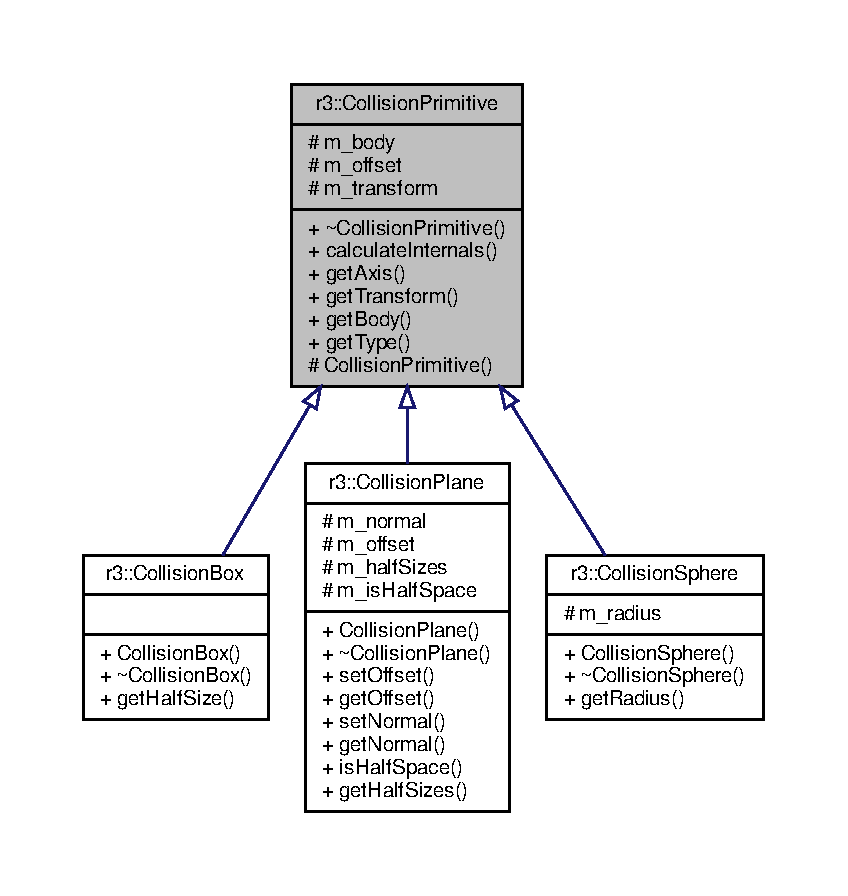
\includegraphics[width=350pt]{classr3_1_1_collision_primitive__inherit__graph}
\end{center}
\end{figure}


Collaboration diagram for r3\+:\+:Collision\+Primitive\+:\nopagebreak
\begin{figure}[H]
\begin{center}
\leavevmode
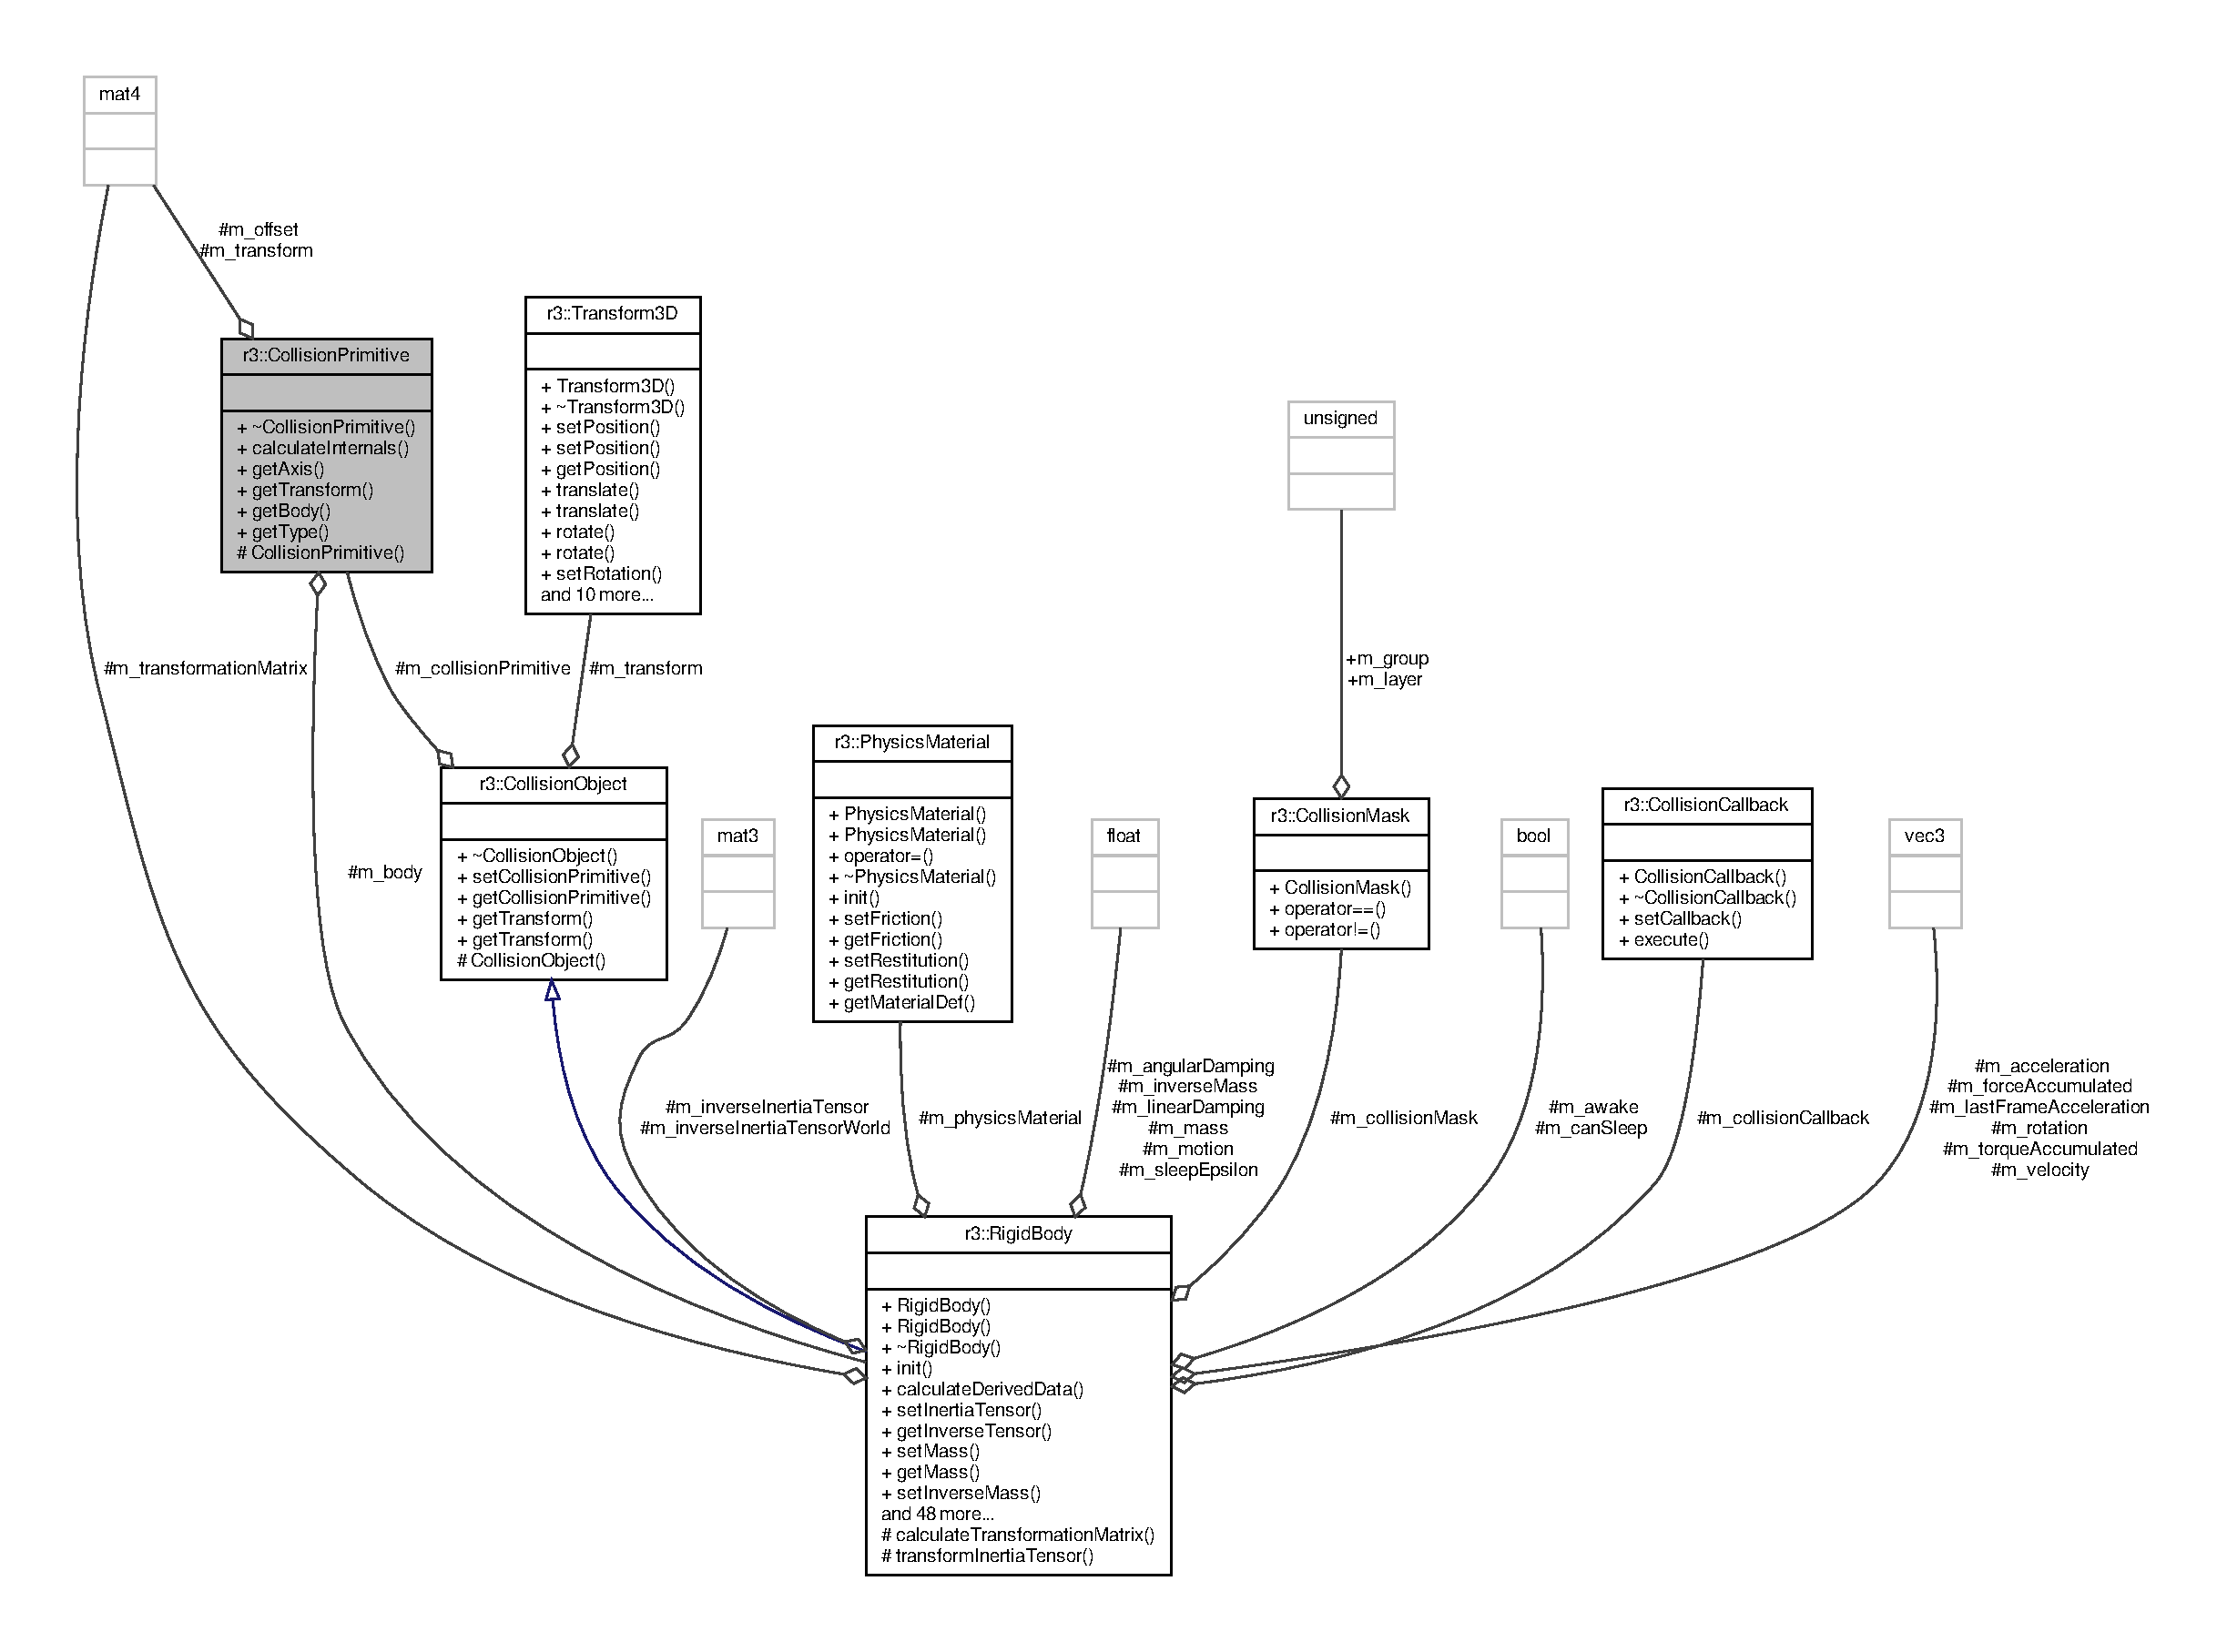
\includegraphics[width=350pt]{classr3_1_1_collision_primitive__coll__graph}
\end{center}
\end{figure}
\subsection*{Public Member Functions}
\begin{DoxyCompactItemize}
\item 
virtual \mbox{\hyperlink{classr3_1_1_collision_primitive_adfa75f14067cb33a3f0049895a3db880}{$\sim$\+Collision\+Primitive}} ()
\item 
void \mbox{\hyperlink{classr3_1_1_collision_primitive_ae27cb70a6812491c2d8de97f22c07ac6}{calculate\+Internals}} ()
\begin{DoxyCompactList}\small\item\em Calculates its transformation. \end{DoxyCompactList}\item 
glm\+::vec3 \mbox{\hyperlink{classr3_1_1_collision_primitive_a78c959f5ca0a09a0fc2038ac7f30e45a}{get\+Axis}} (unsigned index) const
\begin{DoxyCompactList}\small\item\em Get an axis from the transformation matrix. \end{DoxyCompactList}\item 
const glm\+::mat4 \& \mbox{\hyperlink{classr3_1_1_collision_primitive_acc4e2139c698bab280338db36d7cc586}{get\+Transform}} () const
\begin{DoxyCompactList}\small\item\em Get the transform of this primitive. \end{DoxyCompactList}\item 
\mbox{\hyperlink{classr3_1_1_rigid_body}{Rigid\+Body}} $\ast$ \mbox{\hyperlink{classr3_1_1_collision_primitive_af8dbda90cce34a6262309cbdb75feea7}{get\+Body}} () const
\begin{DoxyCompactList}\small\item\em Get the rigid body, which uses this collision primitive. \end{DoxyCompactList}\item 
Collision\+Primitive\+Type \mbox{\hyperlink{classr3_1_1_collision_primitive_ac7a318fb788d1442e7d3390c8e465e14}{get\+Type}} () const
\begin{DoxyCompactList}\small\item\em Get the type of this primitive. \end{DoxyCompactList}\end{DoxyCompactItemize}
\subsection*{Protected Member Functions}
\begin{DoxyCompactItemize}
\item 
\mbox{\hyperlink{classr3_1_1_collision_primitive_a56f4cef84fcb4d92b0ced2ffcefdb22a}{Collision\+Primitive}} (Collision\+Primitive\+Type type)
\begin{DoxyCompactList}\small\item\em \mbox{\hyperlink{classr3_1_1_collision_primitive}{Collision\+Primitive}} constructor. \end{DoxyCompactList}\end{DoxyCompactItemize}
\subsection*{Protected Attributes}
\begin{DoxyCompactItemize}
\item 
\mbox{\hyperlink{classr3_1_1_rigid_body}{Rigid\+Body}} $\ast$ \mbox{\hyperlink{classr3_1_1_collision_primitive_a3ae500c9bd222ec42d86696702e746db}{m\+\_\+body}} \{\}
\begin{DoxyCompactList}\small\item\em The rigid body this collision primitive represents. \end{DoxyCompactList}\item 
glm\+::mat4 \mbox{\hyperlink{classr3_1_1_collision_primitive_a15a51c2e72a8c5122a1031d6620a2901}{m\+\_\+offset}}
\begin{DoxyCompactList}\small\item\em Offset from the represented rigid body. \end{DoxyCompactList}\item 
glm\+::mat4 \mbox{\hyperlink{classr3_1_1_collision_primitive_a0cb28517e7791b9836a5cac5d8550b13}{m\+\_\+transform}}
\end{DoxyCompactItemize}


\subsection{Detailed Description}
Abstract collision shape, which can collide with other collision primitives. 

\subsection{Constructor \& Destructor Documentation}
\mbox{\Hypertarget{classr3_1_1_collision_primitive_adfa75f14067cb33a3f0049895a3db880}\label{classr3_1_1_collision_primitive_adfa75f14067cb33a3f0049895a3db880}} 
\index{r3\+::\+Collision\+Primitive@{r3\+::\+Collision\+Primitive}!````~Collision\+Primitive@{$\sim$\+Collision\+Primitive}}
\index{````~Collision\+Primitive@{$\sim$\+Collision\+Primitive}!r3\+::\+Collision\+Primitive@{r3\+::\+Collision\+Primitive}}
\subsubsection{\texorpdfstring{$\sim$\+Collision\+Primitive()}{~CollisionPrimitive()}}
{\footnotesize\ttfamily r3\+::\+Collision\+Primitive\+::$\sim$\+Collision\+Primitive (\begin{DoxyParamCaption}{ }\end{DoxyParamCaption})\hspace{0.3cm}{\ttfamily [virtual]}, {\ttfamily [default]}}

\mbox{\Hypertarget{classr3_1_1_collision_primitive_a56f4cef84fcb4d92b0ced2ffcefdb22a}\label{classr3_1_1_collision_primitive_a56f4cef84fcb4d92b0ced2ffcefdb22a}} 
\index{r3\+::\+Collision\+Primitive@{r3\+::\+Collision\+Primitive}!Collision\+Primitive@{Collision\+Primitive}}
\index{Collision\+Primitive@{Collision\+Primitive}!r3\+::\+Collision\+Primitive@{r3\+::\+Collision\+Primitive}}
\subsubsection{\texorpdfstring{Collision\+Primitive()}{CollisionPrimitive()}}
{\footnotesize\ttfamily r3\+::\+Collision\+Primitive\+::\+Collision\+Primitive (\begin{DoxyParamCaption}\item[{Collision\+Primitive\+Type}]{type }\end{DoxyParamCaption})\hspace{0.3cm}{\ttfamily [explicit]}, {\ttfamily [protected]}}



\mbox{\hyperlink{classr3_1_1_collision_primitive}{Collision\+Primitive}} constructor. 


\begin{DoxyParams}{Parameters}
{\em type} & The type of the primitive. \\
\hline
\end{DoxyParams}


\subsection{Member Function Documentation}
\mbox{\Hypertarget{classr3_1_1_collision_primitive_ae27cb70a6812491c2d8de97f22c07ac6}\label{classr3_1_1_collision_primitive_ae27cb70a6812491c2d8de97f22c07ac6}} 
\index{r3\+::\+Collision\+Primitive@{r3\+::\+Collision\+Primitive}!calculate\+Internals@{calculate\+Internals}}
\index{calculate\+Internals@{calculate\+Internals}!r3\+::\+Collision\+Primitive@{r3\+::\+Collision\+Primitive}}
\subsubsection{\texorpdfstring{calculate\+Internals()}{calculateInternals()}}
{\footnotesize\ttfamily void r3\+::\+Collision\+Primitive\+::calculate\+Internals (\begin{DoxyParamCaption}{ }\end{DoxyParamCaption})}



Calculates its transformation. 

\begin{DoxyRefDesc}{Todo}
\item[\mbox{\hyperlink{todo__todo000015}{Todo}}]use new transform! \end{DoxyRefDesc}
\mbox{\Hypertarget{classr3_1_1_collision_primitive_a78c959f5ca0a09a0fc2038ac7f30e45a}\label{classr3_1_1_collision_primitive_a78c959f5ca0a09a0fc2038ac7f30e45a}} 
\index{r3\+::\+Collision\+Primitive@{r3\+::\+Collision\+Primitive}!get\+Axis@{get\+Axis}}
\index{get\+Axis@{get\+Axis}!r3\+::\+Collision\+Primitive@{r3\+::\+Collision\+Primitive}}
\subsubsection{\texorpdfstring{get\+Axis()}{getAxis()}}
{\footnotesize\ttfamily glm\+::vec3 r3\+::\+Collision\+Primitive\+::get\+Axis (\begin{DoxyParamCaption}\item[{unsigned}]{index }\end{DoxyParamCaption}) const}



Get an axis from the transformation matrix. 


\begin{DoxyParams}{Parameters}
{\em index} & The index of the axis. \\
\hline
\end{DoxyParams}
\begin{DoxyReturn}{Returns}
The axis; 
\end{DoxyReturn}
\mbox{\Hypertarget{classr3_1_1_collision_primitive_af8dbda90cce34a6262309cbdb75feea7}\label{classr3_1_1_collision_primitive_af8dbda90cce34a6262309cbdb75feea7}} 
\index{r3\+::\+Collision\+Primitive@{r3\+::\+Collision\+Primitive}!get\+Body@{get\+Body}}
\index{get\+Body@{get\+Body}!r3\+::\+Collision\+Primitive@{r3\+::\+Collision\+Primitive}}
\subsubsection{\texorpdfstring{get\+Body()}{getBody()}}
{\footnotesize\ttfamily \mbox{\hyperlink{classr3_1_1_rigid_body}{Rigid\+Body}} $\ast$ r3\+::\+Collision\+Primitive\+::get\+Body (\begin{DoxyParamCaption}{ }\end{DoxyParamCaption}) const}



Get the rigid body, which uses this collision primitive. 

\begin{DoxyReturn}{Returns}
The rigid body. 
\end{DoxyReturn}
\mbox{\Hypertarget{classr3_1_1_collision_primitive_acc4e2139c698bab280338db36d7cc586}\label{classr3_1_1_collision_primitive_acc4e2139c698bab280338db36d7cc586}} 
\index{r3\+::\+Collision\+Primitive@{r3\+::\+Collision\+Primitive}!get\+Transform@{get\+Transform}}
\index{get\+Transform@{get\+Transform}!r3\+::\+Collision\+Primitive@{r3\+::\+Collision\+Primitive}}
\subsubsection{\texorpdfstring{get\+Transform()}{getTransform()}}
{\footnotesize\ttfamily const glm\+::mat4 \& r3\+::\+Collision\+Primitive\+::get\+Transform (\begin{DoxyParamCaption}{ }\end{DoxyParamCaption}) const}



Get the transform of this primitive. 

\begin{DoxyReturn}{Returns}
The transform. 
\end{DoxyReturn}
\mbox{\Hypertarget{classr3_1_1_collision_primitive_ac7a318fb788d1442e7d3390c8e465e14}\label{classr3_1_1_collision_primitive_ac7a318fb788d1442e7d3390c8e465e14}} 
\index{r3\+::\+Collision\+Primitive@{r3\+::\+Collision\+Primitive}!get\+Type@{get\+Type}}
\index{get\+Type@{get\+Type}!r3\+::\+Collision\+Primitive@{r3\+::\+Collision\+Primitive}}
\subsubsection{\texorpdfstring{get\+Type()}{getType()}}
{\footnotesize\ttfamily Collision\+Primitive\+Type r3\+::\+Collision\+Primitive\+::get\+Type (\begin{DoxyParamCaption}{ }\end{DoxyParamCaption}) const}



Get the type of this primitive. 

\begin{DoxyReturn}{Returns}
The primitive specific type. 
\end{DoxyReturn}


\subsection{Member Data Documentation}
\mbox{\Hypertarget{classr3_1_1_collision_primitive_a3ae500c9bd222ec42d86696702e746db}\label{classr3_1_1_collision_primitive_a3ae500c9bd222ec42d86696702e746db}} 
\index{r3\+::\+Collision\+Primitive@{r3\+::\+Collision\+Primitive}!m\+\_\+body@{m\+\_\+body}}
\index{m\+\_\+body@{m\+\_\+body}!r3\+::\+Collision\+Primitive@{r3\+::\+Collision\+Primitive}}
\subsubsection{\texorpdfstring{m\+\_\+body}{m\_body}}
{\footnotesize\ttfamily \mbox{\hyperlink{classr3_1_1_rigid_body}{Rigid\+Body}}$\ast$ r3\+::\+Collision\+Primitive\+::m\+\_\+body \{\}\hspace{0.3cm}{\ttfamily [protected]}}



The rigid body this collision primitive represents. 

\mbox{\Hypertarget{classr3_1_1_collision_primitive_a15a51c2e72a8c5122a1031d6620a2901}\label{classr3_1_1_collision_primitive_a15a51c2e72a8c5122a1031d6620a2901}} 
\index{r3\+::\+Collision\+Primitive@{r3\+::\+Collision\+Primitive}!m\+\_\+offset@{m\+\_\+offset}}
\index{m\+\_\+offset@{m\+\_\+offset}!r3\+::\+Collision\+Primitive@{r3\+::\+Collision\+Primitive}}
\subsubsection{\texorpdfstring{m\+\_\+offset}{m\_offset}}
{\footnotesize\ttfamily glm\+::mat4 r3\+::\+Collision\+Primitive\+::m\+\_\+offset\hspace{0.3cm}{\ttfamily [protected]}}



Offset from the represented rigid body. 

\mbox{\Hypertarget{classr3_1_1_collision_primitive_a0cb28517e7791b9836a5cac5d8550b13}\label{classr3_1_1_collision_primitive_a0cb28517e7791b9836a5cac5d8550b13}} 
\index{r3\+::\+Collision\+Primitive@{r3\+::\+Collision\+Primitive}!m\+\_\+transform@{m\+\_\+transform}}
\index{m\+\_\+transform@{m\+\_\+transform}!r3\+::\+Collision\+Primitive@{r3\+::\+Collision\+Primitive}}
\subsubsection{\texorpdfstring{m\+\_\+transform}{m\_transform}}
{\footnotesize\ttfamily glm\+::mat4 r3\+::\+Collision\+Primitive\+::m\+\_\+transform\hspace{0.3cm}{\ttfamily [protected]}}



The documentation for this class was generated from the following files\+:\begin{DoxyCompactItemize}
\item 
D\+:/\+Library/\+Documents/\+Job/\+Forschungsmaster/\+Projekte/\+Simulation\+Visualization/\+Rumble3\+D/\+Rumble3\+D/include/\+R3\+D/\+Rigid\+Body\+Engine/\mbox{\hyperlink{_collision_primitive_8h}{Collision\+Primitive.\+h}}\item 
D\+:/\+Library/\+Documents/\+Job/\+Forschungsmaster/\+Projekte/\+Simulation\+Visualization/\+Rumble3\+D/\+Rumble3\+D/src/\+Rigid\+Body\+Engine/\mbox{\hyperlink{_collision_primitive_8cpp}{Collision\+Primitive.\+cpp}}\end{DoxyCompactItemize}

\hypertarget{classr3_1_1_collision_resolver}{}\doxysection{r3\+::Collision\+Resolver Class Reference}
\label{classr3_1_1_collision_resolver}\index{r3::CollisionResolver@{r3::CollisionResolver}}


Default implementation for a collision resolver.  




{\ttfamily \#include $<$Collision\+Resolver.\+h$>$}



Inheritance diagram for r3\+::Collision\+Resolver\+:\nopagebreak
\begin{figure}[H]
\begin{center}
\leavevmode
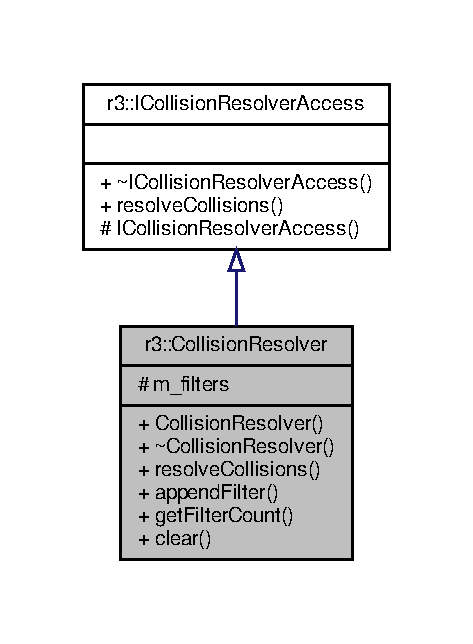
\includegraphics[width=227pt]{classr3_1_1_collision_resolver__inherit__graph}
\end{center}
\end{figure}


Collaboration diagram for r3\+::Collision\+Resolver\+:\nopagebreak
\begin{figure}[H]
\begin{center}
\leavevmode
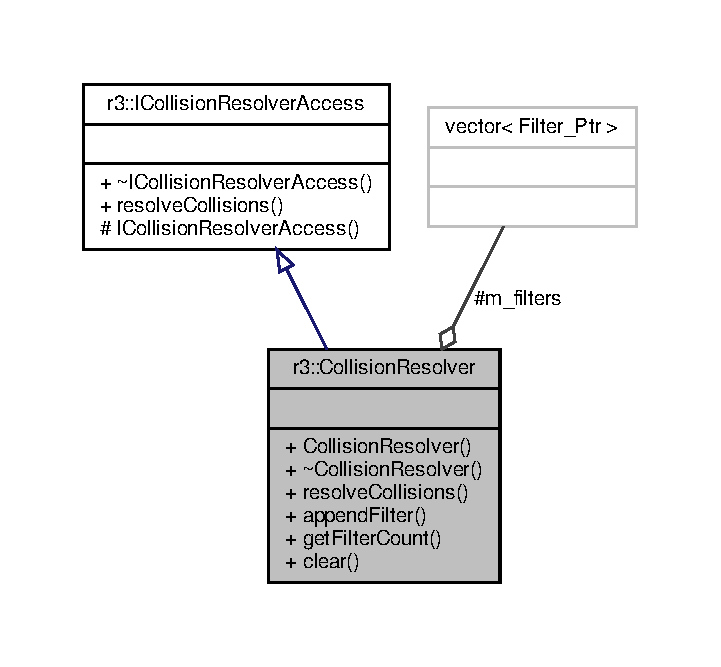
\includegraphics[width=346pt]{classr3_1_1_collision_resolver__coll__graph}
\end{center}
\end{figure}
\doxysubsection*{Public Types}
\begin{DoxyCompactItemize}
\item 
using \mbox{\hyperlink{classr3_1_1_collision_resolver_a5b3838b81de7909c3c78268801d61414}{Filter\+\_\+\+Ptr}} = std\+::shared\+\_\+ptr$<$ \mbox{\hyperlink{classr3_1_1_i_collision_resolution_filter}{I\+Collision\+Resolution\+Filter}} $>$
\end{DoxyCompactItemize}
\doxysubsection*{Public Member Functions}
\begin{DoxyCompactItemize}
\item 
\mbox{\hyperlink{classr3_1_1_collision_resolver_a7b90e276403fa8422879228a189432fb}{Collision\+Resolver}} ()
\item 
virtual \mbox{\hyperlink{classr3_1_1_collision_resolver_ad172d58efecf5ef38f42020f21746f02}{$\sim$\+Collision\+Resolver}} ()
\item 
void \mbox{\hyperlink{classr3_1_1_collision_resolver_a134da5221d60b34c568f7de29c9d0a58}{resolve\+Collisions}} (\mbox{\hyperlink{classr3_1_1_collision_data}{Collision\+Data}} \&collision\+Data, \mbox{\hyperlink{namespacer3_ab2016b3e3f743fb735afce242f0dc1eb}{real}} time\+Delta) override
\item 
\mbox{\hyperlink{classr3_1_1_i_collision_resolution_filter}{I\+Collision\+Resolution\+Filter}} $\ast$ \mbox{\hyperlink{classr3_1_1_collision_resolver_adad2e36c48000a5af14b679fde5e7b3d}{append\+Filter}} (const \mbox{\hyperlink{classr3_1_1_collision_resolver_a5b3838b81de7909c3c78268801d61414}{Filter\+\_\+\+Ptr}} \&filter)
\begin{DoxyCompactList}\small\item\em Insert a new filter, which will be executed after all already inserted filters. \end{DoxyCompactList}\item 
unsigned int \mbox{\hyperlink{classr3_1_1_collision_resolver_ae56e2125e24982ad368f0d87e9c2a28f}{get\+Filter\+Count}} () const
\item 
void \mbox{\hyperlink{classr3_1_1_collision_resolver_a1f4e3d97afae66c03581807a529678cd}{clear}} ()
\end{DoxyCompactItemize}
\doxysubsection*{Protected Attributes}
\begin{DoxyCompactItemize}
\item 
std\+::vector$<$ \mbox{\hyperlink{classr3_1_1_collision_resolver_a5b3838b81de7909c3c78268801d61414}{Filter\+\_\+\+Ptr}} $>$ \mbox{\hyperlink{classr3_1_1_collision_resolver_abf1234ad45ba7f114b31950c90ccaaff}{m\+\_\+filters}}
\end{DoxyCompactItemize}
\doxysubsection*{Additional Inherited Members}


\doxysubsection{Detailed Description}
Default implementation for a collision resolver. 

\doxysubsection{Member Typedef Documentation}
\mbox{\Hypertarget{classr3_1_1_collision_resolver_a5b3838b81de7909c3c78268801d61414}\label{classr3_1_1_collision_resolver_a5b3838b81de7909c3c78268801d61414}} 
\index{r3::CollisionResolver@{r3::CollisionResolver}!Filter\_Ptr@{Filter\_Ptr}}
\index{Filter\_Ptr@{Filter\_Ptr}!r3::CollisionResolver@{r3::CollisionResolver}}
\doxysubsubsection{\texorpdfstring{Filter\_Ptr}{Filter\_Ptr}}
{\footnotesize\ttfamily using \mbox{\hyperlink{classr3_1_1_collision_resolver_a5b3838b81de7909c3c78268801d61414}{r3\+::\+Collision\+Resolver\+::\+Filter\+\_\+\+Ptr}} =  std\+::shared\+\_\+ptr$<$\mbox{\hyperlink{classr3_1_1_i_collision_resolution_filter}{I\+Collision\+Resolution\+Filter}}$>$}



\doxysubsection{Constructor \& Destructor Documentation}
\mbox{\Hypertarget{classr3_1_1_collision_resolver_a7b90e276403fa8422879228a189432fb}\label{classr3_1_1_collision_resolver_a7b90e276403fa8422879228a189432fb}} 
\index{r3::CollisionResolver@{r3::CollisionResolver}!CollisionResolver@{CollisionResolver}}
\index{CollisionResolver@{CollisionResolver}!r3::CollisionResolver@{r3::CollisionResolver}}
\doxysubsubsection{\texorpdfstring{CollisionResolver()}{CollisionResolver()}}
{\footnotesize\ttfamily r3\+::\+Collision\+Resolver\+::\+Collision\+Resolver (\begin{DoxyParamCaption}{ }\end{DoxyParamCaption})\hspace{0.3cm}{\ttfamily [explicit]}}

\mbox{\Hypertarget{classr3_1_1_collision_resolver_ad172d58efecf5ef38f42020f21746f02}\label{classr3_1_1_collision_resolver_ad172d58efecf5ef38f42020f21746f02}} 
\index{r3::CollisionResolver@{r3::CollisionResolver}!````~CollisionResolver@{$\sim$CollisionResolver}}
\index{````~CollisionResolver@{$\sim$CollisionResolver}!r3::CollisionResolver@{r3::CollisionResolver}}
\doxysubsubsection{\texorpdfstring{$\sim$CollisionResolver()}{~CollisionResolver()}}
{\footnotesize\ttfamily r3\+::\+Collision\+Resolver\+::$\sim$\+Collision\+Resolver (\begin{DoxyParamCaption}{ }\end{DoxyParamCaption})\hspace{0.3cm}{\ttfamily [virtual]}, {\ttfamily [default]}}



\doxysubsection{Member Function Documentation}
\mbox{\Hypertarget{classr3_1_1_collision_resolver_adad2e36c48000a5af14b679fde5e7b3d}\label{classr3_1_1_collision_resolver_adad2e36c48000a5af14b679fde5e7b3d}} 
\index{r3::CollisionResolver@{r3::CollisionResolver}!appendFilter@{appendFilter}}
\index{appendFilter@{appendFilter}!r3::CollisionResolver@{r3::CollisionResolver}}
\doxysubsubsection{\texorpdfstring{appendFilter()}{appendFilter()}}
{\footnotesize\ttfamily \mbox{\hyperlink{classr3_1_1_i_collision_resolution_filter}{I\+Collision\+Resolution\+Filter}} $\ast$ r3\+::\+Collision\+Resolver\+::append\+Filter (\begin{DoxyParamCaption}\item[{const \mbox{\hyperlink{classr3_1_1_collision_resolver_a5b3838b81de7909c3c78268801d61414}{Filter\+\_\+\+Ptr}} \&}]{filter }\end{DoxyParamCaption})}



Insert a new filter, which will be executed after all already inserted filters. 


\begin{DoxyParams}{Parameters}
{\em filter} & The new filter. \\
\hline
\end{DoxyParams}
\begin{DoxyReturn}{Returns}
The new filter. 
\end{DoxyReturn}
\mbox{\Hypertarget{classr3_1_1_collision_resolver_a1f4e3d97afae66c03581807a529678cd}\label{classr3_1_1_collision_resolver_a1f4e3d97afae66c03581807a529678cd}} 
\index{r3::CollisionResolver@{r3::CollisionResolver}!clear@{clear}}
\index{clear@{clear}!r3::CollisionResolver@{r3::CollisionResolver}}
\doxysubsubsection{\texorpdfstring{clear()}{clear()}}
{\footnotesize\ttfamily void r3\+::\+Collision\+Resolver\+::clear (\begin{DoxyParamCaption}{ }\end{DoxyParamCaption})}

Removes all filters from this collision resolver. \mbox{\Hypertarget{classr3_1_1_collision_resolver_ae56e2125e24982ad368f0d87e9c2a28f}\label{classr3_1_1_collision_resolver_ae56e2125e24982ad368f0d87e9c2a28f}} 
\index{r3::CollisionResolver@{r3::CollisionResolver}!getFilterCount@{getFilterCount}}
\index{getFilterCount@{getFilterCount}!r3::CollisionResolver@{r3::CollisionResolver}}
\doxysubsubsection{\texorpdfstring{getFilterCount()}{getFilterCount()}}
{\footnotesize\ttfamily unsigned r3\+::\+Collision\+Resolver\+::get\+Filter\+Count (\begin{DoxyParamCaption}{ }\end{DoxyParamCaption}) const}

Get the current number of used filters. \mbox{\Hypertarget{classr3_1_1_collision_resolver_a134da5221d60b34c568f7de29c9d0a58}\label{classr3_1_1_collision_resolver_a134da5221d60b34c568f7de29c9d0a58}} 
\index{r3::CollisionResolver@{r3::CollisionResolver}!resolveCollisions@{resolveCollisions}}
\index{resolveCollisions@{resolveCollisions}!r3::CollisionResolver@{r3::CollisionResolver}}
\doxysubsubsection{\texorpdfstring{resolveCollisions()}{resolveCollisions()}}
{\footnotesize\ttfamily void r3\+::\+Collision\+Resolver\+::resolve\+Collisions (\begin{DoxyParamCaption}\item[{\mbox{\hyperlink{classr3_1_1_collision_data}{Collision\+Data}} \&}]{collision\+Data,  }\item[{\mbox{\hyperlink{namespacer3_ab2016b3e3f743fb735afce242f0dc1eb}{real}}}]{time\+Delta }\end{DoxyParamCaption})\hspace{0.3cm}{\ttfamily [override]}, {\ttfamily [virtual]}}



Implements \mbox{\hyperlink{classr3_1_1_i_collision_resolver_access_a266dfbc4c421a7c3429ef474d63fd941}{r3\+::\+I\+Collision\+Resolver\+Access}}.



\doxysubsection{Member Data Documentation}
\mbox{\Hypertarget{classr3_1_1_collision_resolver_abf1234ad45ba7f114b31950c90ccaaff}\label{classr3_1_1_collision_resolver_abf1234ad45ba7f114b31950c90ccaaff}} 
\index{r3::CollisionResolver@{r3::CollisionResolver}!m\_filters@{m\_filters}}
\index{m\_filters@{m\_filters}!r3::CollisionResolver@{r3::CollisionResolver}}
\doxysubsubsection{\texorpdfstring{m\_filters}{m\_filters}}
{\footnotesize\ttfamily std\+::vector$<$\mbox{\hyperlink{classr3_1_1_collision_resolver_a5b3838b81de7909c3c78268801d61414}{Filter\+\_\+\+Ptr}}$>$ r3\+::\+Collision\+Resolver\+::m\+\_\+filters\hspace{0.3cm}{\ttfamily [protected]}}



The documentation for this class was generated from the following files\+:\begin{DoxyCompactItemize}
\item 
/home/nelaty/\+Development/\+Repositories/\+Rumble3\+D/include/\+R3\+D/\+Rigid\+Body\+Engine/\+Collision\+Resolution/\mbox{\hyperlink{_collision_resolver_8h}{Collision\+Resolver.\+h}}\item 
/home/nelaty/\+Development/\+Repositories/\+Rumble3\+D/src/\+Rigid\+Body\+Engine/\+Collision\+Resolution/\mbox{\hyperlink{_collision_resolver_8cpp}{Collision\+Resolver.\+cpp}}\end{DoxyCompactItemize}

\hypertarget{classr3_1_1_collision_sphere}{}\doxysection{r3\+::Collision\+Sphere Class Reference}
\label{classr3_1_1_collision_sphere}\index{r3::CollisionSphere@{r3::CollisionSphere}}


\mbox{\hyperlink{classr3_1_1_collision_primitive}{Collision\+Primitive}}, which represents a sphere.  




{\ttfamily \#include $<$Collision\+Sphere.\+h$>$}



Inheritance diagram for r3\+::Collision\+Sphere\+:\nopagebreak
\begin{figure}[H]
\begin{center}
\leavevmode
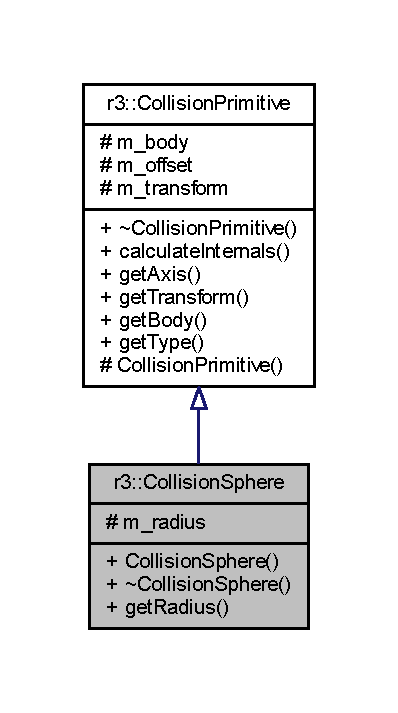
\includegraphics[width=191pt]{classr3_1_1_collision_sphere__inherit__graph}
\end{center}
\end{figure}


Collaboration diagram for r3\+::Collision\+Sphere\+:\nopagebreak
\begin{figure}[H]
\begin{center}
\leavevmode
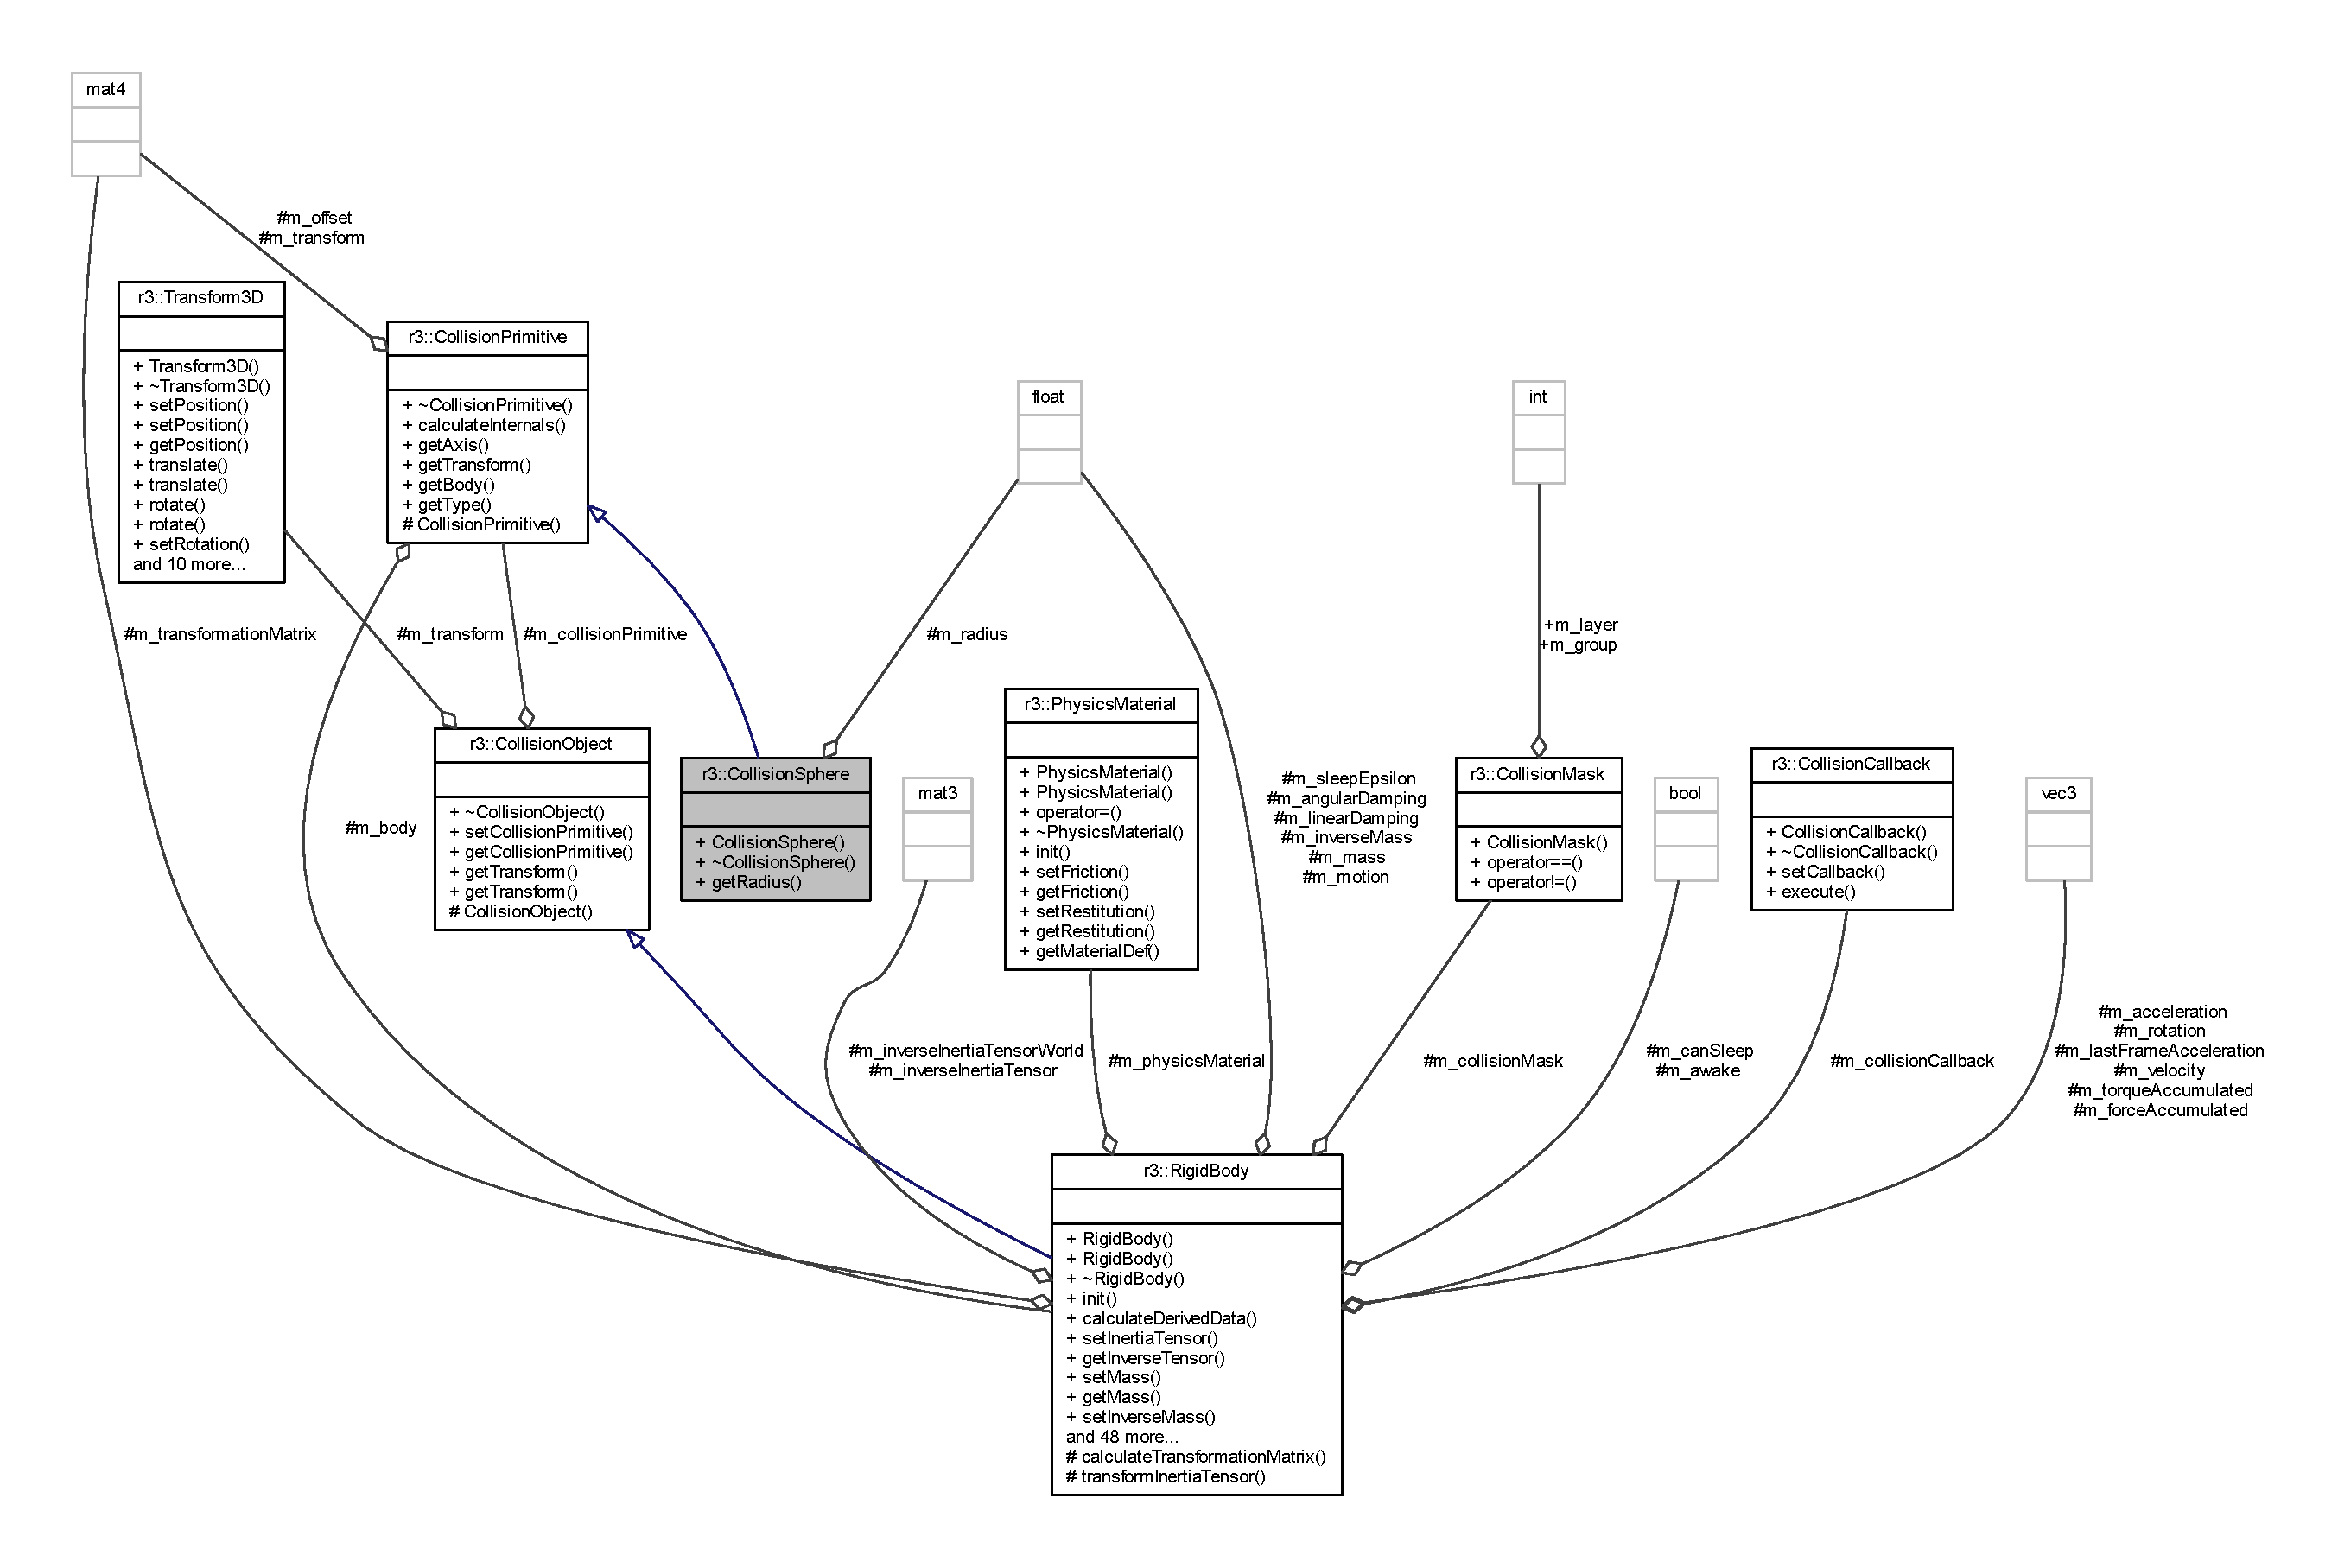
\includegraphics[width=350pt]{classr3_1_1_collision_sphere__coll__graph}
\end{center}
\end{figure}
\doxysubsection*{Public Member Functions}
\begin{DoxyCompactItemize}
\item 
\mbox{\hyperlink{classr3_1_1_collision_sphere_a3b910b66d6b9689da9beba5ec151eba3}{Collision\+Sphere}} (\mbox{\hyperlink{classr3_1_1_rigid_body}{Rigid\+Body}} $\ast$body, \mbox{\hyperlink{namespacer3_ab2016b3e3f743fb735afce242f0dc1eb}{real}} radius, const glm\+::mat4 \&offset=glm\+::mat4(1))
\begin{DoxyCompactList}\small\item\em \mbox{\hyperlink{classr3_1_1_collision_sphere}{Collision\+Sphere}} constructor. \end{DoxyCompactList}\item 
\mbox{\hyperlink{classr3_1_1_collision_sphere_a3605a7afc888411c5fa52179122a8a77}{$\sim$\+Collision\+Sphere}} ()
\item 
\mbox{\hyperlink{namespacer3_ab2016b3e3f743fb735afce242f0dc1eb}{real}} \mbox{\hyperlink{classr3_1_1_collision_sphere_aa3b7687165b34ab82b3bedb0884cc65b}{get\+Radius}} () const
\begin{DoxyCompactList}\small\item\em Get the radius of the collision sphere. \end{DoxyCompactList}\end{DoxyCompactItemize}
\doxysubsection*{Protected Attributes}
\begin{DoxyCompactItemize}
\item 
\mbox{\hyperlink{namespacer3_ab2016b3e3f743fb735afce242f0dc1eb}{real}} \mbox{\hyperlink{classr3_1_1_collision_sphere_abc9e3dcae422b4732a288fa19d89d466}{m\+\_\+radius}}
\end{DoxyCompactItemize}
\doxysubsection*{Additional Inherited Members}


\doxysubsection{Detailed Description}
\mbox{\hyperlink{classr3_1_1_collision_primitive}{Collision\+Primitive}}, which represents a sphere. 

\doxysubsection{Constructor \& Destructor Documentation}
\mbox{\Hypertarget{classr3_1_1_collision_sphere_a3b910b66d6b9689da9beba5ec151eba3}\label{classr3_1_1_collision_sphere_a3b910b66d6b9689da9beba5ec151eba3}} 
\index{r3::CollisionSphere@{r3::CollisionSphere}!CollisionSphere@{CollisionSphere}}
\index{CollisionSphere@{CollisionSphere}!r3::CollisionSphere@{r3::CollisionSphere}}
\doxysubsubsection{\texorpdfstring{CollisionSphere()}{CollisionSphere()}}
{\footnotesize\ttfamily r3\+::\+Collision\+Sphere\+::\+Collision\+Sphere (\begin{DoxyParamCaption}\item[{\mbox{\hyperlink{classr3_1_1_rigid_body}{Rigid\+Body}} $\ast$}]{body,  }\item[{\mbox{\hyperlink{namespacer3_ab2016b3e3f743fb735afce242f0dc1eb}{real}}}]{radius,  }\item[{const glm\+::mat4 \&}]{offset = {\ttfamily glm\+:\+:mat4(1)} }\end{DoxyParamCaption})}



\mbox{\hyperlink{classr3_1_1_collision_sphere}{Collision\+Sphere}} constructor. 


\begin{DoxyParams}{Parameters}
{\em body} & The rigid body this collision sphere represents. \\
\hline
{\em radius} & The radius of the collision sphere. \\
\hline
{\em offset} & Offset from the represented rigid body. \\
\hline
\end{DoxyParams}
\mbox{\Hypertarget{classr3_1_1_collision_sphere_a3605a7afc888411c5fa52179122a8a77}\label{classr3_1_1_collision_sphere_a3605a7afc888411c5fa52179122a8a77}} 
\index{r3::CollisionSphere@{r3::CollisionSphere}!````~CollisionSphere@{$\sim$CollisionSphere}}
\index{````~CollisionSphere@{$\sim$CollisionSphere}!r3::CollisionSphere@{r3::CollisionSphere}}
\doxysubsubsection{\texorpdfstring{$\sim$CollisionSphere()}{~CollisionSphere()}}
{\footnotesize\ttfamily r3\+::\+Collision\+Sphere\+::$\sim$\+Collision\+Sphere (\begin{DoxyParamCaption}{ }\end{DoxyParamCaption})\hspace{0.3cm}{\ttfamily [default]}}



\doxysubsection{Member Function Documentation}
\mbox{\Hypertarget{classr3_1_1_collision_sphere_aa3b7687165b34ab82b3bedb0884cc65b}\label{classr3_1_1_collision_sphere_aa3b7687165b34ab82b3bedb0884cc65b}} 
\index{r3::CollisionSphere@{r3::CollisionSphere}!getRadius@{getRadius}}
\index{getRadius@{getRadius}!r3::CollisionSphere@{r3::CollisionSphere}}
\doxysubsubsection{\texorpdfstring{getRadius()}{getRadius()}}
{\footnotesize\ttfamily \mbox{\hyperlink{namespacer3_ab2016b3e3f743fb735afce242f0dc1eb}{real}} r3\+::\+Collision\+Sphere\+::get\+Radius (\begin{DoxyParamCaption}{ }\end{DoxyParamCaption}) const}



Get the radius of the collision sphere. 

\begin{DoxyReturn}{Returns}
The radius of the sphere. 
\end{DoxyReturn}


\doxysubsection{Member Data Documentation}
\mbox{\Hypertarget{classr3_1_1_collision_sphere_abc9e3dcae422b4732a288fa19d89d466}\label{classr3_1_1_collision_sphere_abc9e3dcae422b4732a288fa19d89d466}} 
\index{r3::CollisionSphere@{r3::CollisionSphere}!m\_radius@{m\_radius}}
\index{m\_radius@{m\_radius}!r3::CollisionSphere@{r3::CollisionSphere}}
\doxysubsubsection{\texorpdfstring{m\_radius}{m\_radius}}
{\footnotesize\ttfamily \mbox{\hyperlink{namespacer3_ab2016b3e3f743fb735afce242f0dc1eb}{real}} r3\+::\+Collision\+Sphere\+::m\+\_\+radius\hspace{0.3cm}{\ttfamily [protected]}}



The documentation for this class was generated from the following files\+:\begin{DoxyCompactItemize}
\item 
/home/nelaty/\+Development/\+Repositories/\+Rumble3\+D/include/\+R3\+D/\+Rigid\+Body\+Engine/\mbox{\hyperlink{_collision_sphere_8h}{Collision\+Sphere.\+h}}\item 
/home/nelaty/\+Development/\+Repositories/\+Rumble3\+D/src/\+Rigid\+Body\+Engine/\mbox{\hyperlink{_collision_sphere_8cpp}{Collision\+Sphere.\+cpp}}\end{DoxyCompactItemize}

\hypertarget{classr3_1_1_contact}{}\section{r3\+:\+:Contact Class Reference}
\label{classr3_1_1_contact}\index{r3\+::\+Contact@{r3\+::\+Contact}}


A \mbox{\hyperlink{classr3_1_1_contact}{Contact}} represents a point in space at which two rigid bodies collide. It is not a point in world space but rather knows the relative offsets to the points of mass of both rigid bodies.  




{\ttfamily \#include $<$Contact.\+h$>$}



Collaboration diagram for r3\+:\+:Contact\+:\nopagebreak
\begin{figure}[H]
\begin{center}
\leavevmode
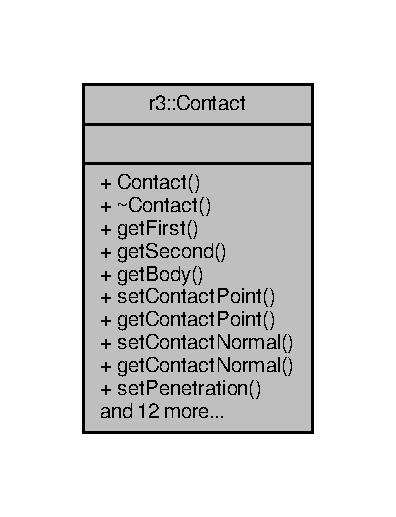
\includegraphics[width=190pt]{classr3_1_1_contact__coll__graph}
\end{center}
\end{figure}
\subsection*{Public Member Functions}
\begin{DoxyCompactItemize}
\item 
\mbox{\hyperlink{classr3_1_1_contact_af2648c9a1e37583ac230a40f4fc6b72d}{Contact}} ()
\item 
\mbox{\hyperlink{classr3_1_1_contact_a011905bfa1cfa3ed459650796b105c6a}{$\sim$\+Contact}} ()
\item 
\mbox{\hyperlink{classr3_1_1_rigid_body}{Rigid\+Body}} $\ast$ \mbox{\hyperlink{classr3_1_1_contact_adf157981ebfd1552521afe7b25e9239c}{get\+First}} () const
\begin{DoxyCompactList}\small\item\em Get the first colliding rigid body. \end{DoxyCompactList}\item 
\mbox{\hyperlink{classr3_1_1_rigid_body}{Rigid\+Body}} $\ast$ \mbox{\hyperlink{classr3_1_1_contact_a90af8f5c7cba65a6a84c57b5a6ef6d70}{get\+Second}} () const
\begin{DoxyCompactList}\small\item\em Get the second colliding rigid body. \end{DoxyCompactList}\item 
\mbox{\hyperlink{classr3_1_1_rigid_body}{Rigid\+Body}} $\ast$ \mbox{\hyperlink{classr3_1_1_contact_aaa7c4c676fd8f3b07f81cc18257c48d9}{get\+Body}} (int index) const
\item 
void \mbox{\hyperlink{classr3_1_1_contact_aedd044892a1adf0692b7cc9f81b4436a}{set\+Contact\+Point}} (const glm\+::vec3 \&contact\+Point)
\begin{DoxyCompactList}\small\item\em Set the contact point. \end{DoxyCompactList}\item 
const glm\+::vec3 \& \mbox{\hyperlink{classr3_1_1_contact_a9558ff3dd4e2c5331fc05076e4e503a0}{get\+Contact\+Point}} () const
\begin{DoxyCompactList}\small\item\em Get the point, where the collision took place. \end{DoxyCompactList}\item 
void \mbox{\hyperlink{classr3_1_1_contact_af7866e211b169ce6565d3f37af8ef8d7}{set\+Contact\+Normal}} (const glm\+::vec3 \&contact\+Normal)
\begin{DoxyCompactList}\small\item\em Set the contact normal. \end{DoxyCompactList}\item 
glm\+::vec3 \mbox{\hyperlink{classr3_1_1_contact_a2d8f594947a1900fd21e2f707384d9fe}{get\+Contact\+Normal}} () const
\begin{DoxyCompactList}\small\item\em Get the contact normal. \end{DoxyCompactList}\item 
void \mbox{\hyperlink{classr3_1_1_contact_a828feb22ff02fe787739eb5d87cfec38}{set\+Penetration}} (\mbox{\hyperlink{namespacer3_ab2016b3e3f743fb735afce242f0dc1eb}{real}} penetration)
\begin{DoxyCompactList}\small\item\em Set the amount of interpenetration. \end{DoxyCompactList}\item 
\mbox{\hyperlink{namespacer3_ab2016b3e3f743fb735afce242f0dc1eb}{real}} \mbox{\hyperlink{classr3_1_1_contact_afe0f0a9a42b4b1f8bd8a61f0b6a4afdd}{get\+Penetration}} () const
\begin{DoxyCompactList}\small\item\em Get the amount of interpenetration. \end{DoxyCompactList}\item 
void \mbox{\hyperlink{classr3_1_1_contact_a7471ab195f0cadaee4e2f27f15bb9fff}{set\+Body\+Data}} (\mbox{\hyperlink{classr3_1_1_rigid_body}{Rigid\+Body}} $\ast$first, \mbox{\hyperlink{classr3_1_1_rigid_body}{Rigid\+Body}} $\ast$second)
\begin{DoxyCompactList}\small\item\em Initialize this contact. \end{DoxyCompactList}\item 
\mbox{\hyperlink{namespacer3_ab2016b3e3f743fb735afce242f0dc1eb}{real}} \mbox{\hyperlink{classr3_1_1_contact_a1a547c3852733960001cc5fe0fe06790}{get\+Friction}} () const
\begin{DoxyCompactList}\small\item\em Get the friction constant used for the bodies in this contact. \end{DoxyCompactList}\item 
\mbox{\hyperlink{namespacer3_ab2016b3e3f743fb735afce242f0dc1eb}{real}} \mbox{\hyperlink{classr3_1_1_contact_a8ec701dcaf82e7fc65bc6c4a2cb6987e}{get\+Restitution}} () const
\begin{DoxyCompactList}\small\item\em Get the restitution constant used for the bodies in this contact. \end{DoxyCompactList}\item 
glm\+::vec3 \mbox{\hyperlink{classr3_1_1_contact_a4c02edbc7514fbc84cd1b7d70797619c}{get\+Closing\+Velocity}} () const
\begin{DoxyCompactList}\small\item\em Get the direction and magnitude of the velocity at which both bodies collided. \end{DoxyCompactList}\item 
void \mbox{\hyperlink{classr3_1_1_contact_a7b837cd82d64d93ce1a98cdd172dd868}{set\+Closing\+Velocity}} (const glm\+::vec3 \&velocity)
\begin{DoxyCompactList}\small\item\em Set the closing velocity at which both bodies collide. \end{DoxyCompactList}\item 
void \mbox{\hyperlink{classr3_1_1_contact_a4e00a32cb21ff4fc8ec826f163bcddae}{calculate\+Internals}} (\mbox{\hyperlink{namespacer3_ab2016b3e3f743fb735afce242f0dc1eb}{real}} duration)
\begin{DoxyCompactList}\small\item\em Prepares this contact for collision resolution. \end{DoxyCompactList}\item 
void \mbox{\hyperlink{classr3_1_1_contact_a3f2c146006389bf6273cdd078763b7a3}{calculate\+Desired\+Delta\+Velocity}} (\mbox{\hyperlink{namespacer3_ab2016b3e3f743fb735afce242f0dc1eb}{real}} duration)
\begin{DoxyCompactList}\small\item\em Calculate the needed velocity for this contact to combat vibrations. \end{DoxyCompactList}\item 
\mbox{\hyperlink{namespacer3_ab2016b3e3f743fb735afce242f0dc1eb}{real}} \mbox{\hyperlink{classr3_1_1_contact_aff234679aa4302b69b8dd101eb969705}{get\+Desired\+Delta\+Velocity}} () const
\begin{DoxyCompactList}\small\item\em Get the needed velocity for this contact to combat vibrations. \end{DoxyCompactList}\item 
const glm\+::vec3 \& \mbox{\hyperlink{classr3_1_1_contact_ade5794f7055fb30ff52f9193b92c6bf0}{get\+Relative\+Contact\+Position}} (int index) const
\begin{DoxyCompactList}\small\item\em Get the contact position relative to the first or the second rigid body. \end{DoxyCompactList}\item 
const glm\+::mat3 \& \mbox{\hyperlink{classr3_1_1_contact_a4e9692d870bdba44ff6b627b8c6c6e30}{get\+Contact\+To\+World}} () const
\begin{DoxyCompactList}\small\item\em Get the rotation matrix, which transforms this contact to world orientation. \end{DoxyCompactList}\item 
void \mbox{\hyperlink{classr3_1_1_contact_a02d78ecc5afe6e7402dd11c655234e4a}{match\+Awake\+State}} ()
\end{DoxyCompactItemize}


\subsection{Detailed Description}
A \mbox{\hyperlink{classr3_1_1_contact}{Contact}} represents a point in space at which two rigid bodies collide. It is not a point in world space but rather knows the relative offsets to the points of mass of both rigid bodies. 

\subsection{Constructor \& Destructor Documentation}
\mbox{\Hypertarget{classr3_1_1_contact_af2648c9a1e37583ac230a40f4fc6b72d}\label{classr3_1_1_contact_af2648c9a1e37583ac230a40f4fc6b72d}} 
\index{r3\+::\+Contact@{r3\+::\+Contact}!Contact@{Contact}}
\index{Contact@{Contact}!r3\+::\+Contact@{r3\+::\+Contact}}
\subsubsection{\texorpdfstring{Contact()}{Contact()}}
{\footnotesize\ttfamily r3\+::\+Contact\+::\+Contact (\begin{DoxyParamCaption}{ }\end{DoxyParamCaption})\hspace{0.3cm}{\ttfamily [explicit]}}

\mbox{\Hypertarget{classr3_1_1_contact_a011905bfa1cfa3ed459650796b105c6a}\label{classr3_1_1_contact_a011905bfa1cfa3ed459650796b105c6a}} 
\index{r3\+::\+Contact@{r3\+::\+Contact}!````~Contact@{$\sim$\+Contact}}
\index{````~Contact@{$\sim$\+Contact}!r3\+::\+Contact@{r3\+::\+Contact}}
\subsubsection{\texorpdfstring{$\sim$\+Contact()}{~Contact()}}
{\footnotesize\ttfamily r3\+::\+Contact\+::$\sim$\+Contact (\begin{DoxyParamCaption}{ }\end{DoxyParamCaption})\hspace{0.3cm}{\ttfamily [default]}}



\subsection{Member Function Documentation}
\mbox{\Hypertarget{classr3_1_1_contact_a3f2c146006389bf6273cdd078763b7a3}\label{classr3_1_1_contact_a3f2c146006389bf6273cdd078763b7a3}} 
\index{r3\+::\+Contact@{r3\+::\+Contact}!calculate\+Desired\+Delta\+Velocity@{calculate\+Desired\+Delta\+Velocity}}
\index{calculate\+Desired\+Delta\+Velocity@{calculate\+Desired\+Delta\+Velocity}!r3\+::\+Contact@{r3\+::\+Contact}}
\subsubsection{\texorpdfstring{calculate\+Desired\+Delta\+Velocity()}{calculateDesiredDeltaVelocity()}}
{\footnotesize\ttfamily void r3\+::\+Contact\+::calculate\+Desired\+Delta\+Velocity (\begin{DoxyParamCaption}\item[{\mbox{\hyperlink{namespacer3_ab2016b3e3f743fb735afce242f0dc1eb}{real}}}]{duration }\end{DoxyParamCaption})}



Calculate the needed velocity for this contact to combat vibrations. 

\mbox{\Hypertarget{classr3_1_1_contact_a4e00a32cb21ff4fc8ec826f163bcddae}\label{classr3_1_1_contact_a4e00a32cb21ff4fc8ec826f163bcddae}} 
\index{r3\+::\+Contact@{r3\+::\+Contact}!calculate\+Internals@{calculate\+Internals}}
\index{calculate\+Internals@{calculate\+Internals}!r3\+::\+Contact@{r3\+::\+Contact}}
\subsubsection{\texorpdfstring{calculate\+Internals()}{calculateInternals()}}
{\footnotesize\ttfamily void r3\+::\+Contact\+::calculate\+Internals (\begin{DoxyParamCaption}\item[{\mbox{\hyperlink{namespacer3_ab2016b3e3f743fb735afce242f0dc1eb}{real}}}]{duration }\end{DoxyParamCaption})}



Prepares this contact for collision resolution. 

Assures that the first rigid body has no infinite mass and swaps it with the second one if necessary. It also calculates the desired delta velocity for this contact as well as the contact velocity and relative contact positions. \mbox{\Hypertarget{classr3_1_1_contact_aaa7c4c676fd8f3b07f81cc18257c48d9}\label{classr3_1_1_contact_aaa7c4c676fd8f3b07f81cc18257c48d9}} 
\index{r3\+::\+Contact@{r3\+::\+Contact}!get\+Body@{get\+Body}}
\index{get\+Body@{get\+Body}!r3\+::\+Contact@{r3\+::\+Contact}}
\subsubsection{\texorpdfstring{get\+Body()}{getBody()}}
{\footnotesize\ttfamily \mbox{\hyperlink{classr3_1_1_rigid_body}{Rigid\+Body}} $\ast$ r3\+::\+Contact\+::get\+Body (\begin{DoxyParamCaption}\item[{int}]{index }\end{DoxyParamCaption}) const}

Get a rigid body by index. \begin{DoxyReturn}{Returns}
The first body if index == 0, the second one if index == 1. 
\end{DoxyReturn}
\mbox{\Hypertarget{classr3_1_1_contact_a4c02edbc7514fbc84cd1b7d70797619c}\label{classr3_1_1_contact_a4c02edbc7514fbc84cd1b7d70797619c}} 
\index{r3\+::\+Contact@{r3\+::\+Contact}!get\+Closing\+Velocity@{get\+Closing\+Velocity}}
\index{get\+Closing\+Velocity@{get\+Closing\+Velocity}!r3\+::\+Contact@{r3\+::\+Contact}}
\subsubsection{\texorpdfstring{get\+Closing\+Velocity()}{getClosingVelocity()}}
{\footnotesize\ttfamily glm\+::vec3 r3\+::\+Contact\+::get\+Closing\+Velocity (\begin{DoxyParamCaption}{ }\end{DoxyParamCaption}) const}



Get the direction and magnitude of the velocity at which both bodies collided. 

\begin{DoxyReturn}{Returns}
The closing velocity 
\end{DoxyReturn}
\mbox{\Hypertarget{classr3_1_1_contact_a2d8f594947a1900fd21e2f707384d9fe}\label{classr3_1_1_contact_a2d8f594947a1900fd21e2f707384d9fe}} 
\index{r3\+::\+Contact@{r3\+::\+Contact}!get\+Contact\+Normal@{get\+Contact\+Normal}}
\index{get\+Contact\+Normal@{get\+Contact\+Normal}!r3\+::\+Contact@{r3\+::\+Contact}}
\subsubsection{\texorpdfstring{get\+Contact\+Normal()}{getContactNormal()}}
{\footnotesize\ttfamily glm\+::vec3 r3\+::\+Contact\+::get\+Contact\+Normal (\begin{DoxyParamCaption}{ }\end{DoxyParamCaption}) const}



Get the contact normal. 

\begin{DoxyReturn}{Returns}
The direction of the collision at the contact point 
\end{DoxyReturn}
\mbox{\Hypertarget{classr3_1_1_contact_a9558ff3dd4e2c5331fc05076e4e503a0}\label{classr3_1_1_contact_a9558ff3dd4e2c5331fc05076e4e503a0}} 
\index{r3\+::\+Contact@{r3\+::\+Contact}!get\+Contact\+Point@{get\+Contact\+Point}}
\index{get\+Contact\+Point@{get\+Contact\+Point}!r3\+::\+Contact@{r3\+::\+Contact}}
\subsubsection{\texorpdfstring{get\+Contact\+Point()}{getContactPoint()}}
{\footnotesize\ttfamily const glm\+::vec3 \& r3\+::\+Contact\+::get\+Contact\+Point (\begin{DoxyParamCaption}{ }\end{DoxyParamCaption}) const}



Get the point, where the collision took place. 

\begin{DoxyReturn}{Returns}
The contact point 
\end{DoxyReturn}
\mbox{\Hypertarget{classr3_1_1_contact_a4e9692d870bdba44ff6b627b8c6c6e30}\label{classr3_1_1_contact_a4e9692d870bdba44ff6b627b8c6c6e30}} 
\index{r3\+::\+Contact@{r3\+::\+Contact}!get\+Contact\+To\+World@{get\+Contact\+To\+World}}
\index{get\+Contact\+To\+World@{get\+Contact\+To\+World}!r3\+::\+Contact@{r3\+::\+Contact}}
\subsubsection{\texorpdfstring{get\+Contact\+To\+World()}{getContactToWorld()}}
{\footnotesize\ttfamily const glm\+::mat3 \& r3\+::\+Contact\+::get\+Contact\+To\+World (\begin{DoxyParamCaption}{ }\end{DoxyParamCaption}) const}



Get the rotation matrix, which transforms this contact to world orientation. 

\begin{DoxyReturn}{Returns}
The rotation matrix 
\end{DoxyReturn}
\mbox{\Hypertarget{classr3_1_1_contact_aff234679aa4302b69b8dd101eb969705}\label{classr3_1_1_contact_aff234679aa4302b69b8dd101eb969705}} 
\index{r3\+::\+Contact@{r3\+::\+Contact}!get\+Desired\+Delta\+Velocity@{get\+Desired\+Delta\+Velocity}}
\index{get\+Desired\+Delta\+Velocity@{get\+Desired\+Delta\+Velocity}!r3\+::\+Contact@{r3\+::\+Contact}}
\subsubsection{\texorpdfstring{get\+Desired\+Delta\+Velocity()}{getDesiredDeltaVelocity()}}
{\footnotesize\ttfamily \mbox{\hyperlink{namespacer3_ab2016b3e3f743fb735afce242f0dc1eb}{real}} r3\+::\+Contact\+::get\+Desired\+Delta\+Velocity (\begin{DoxyParamCaption}{ }\end{DoxyParamCaption}) const}



Get the needed velocity for this contact to combat vibrations. 

\begin{DoxyReturn}{Returns}
The desired velocity difference. 
\end{DoxyReturn}
\mbox{\Hypertarget{classr3_1_1_contact_adf157981ebfd1552521afe7b25e9239c}\label{classr3_1_1_contact_adf157981ebfd1552521afe7b25e9239c}} 
\index{r3\+::\+Contact@{r3\+::\+Contact}!get\+First@{get\+First}}
\index{get\+First@{get\+First}!r3\+::\+Contact@{r3\+::\+Contact}}
\subsubsection{\texorpdfstring{get\+First()}{getFirst()}}
{\footnotesize\ttfamily \mbox{\hyperlink{classr3_1_1_rigid_body}{Rigid\+Body}} $\ast$ r3\+::\+Contact\+::get\+First (\begin{DoxyParamCaption}{ }\end{DoxyParamCaption}) const}



Get the first colliding rigid body. 

\begin{DoxyReturn}{Returns}
The first rigid body 
\end{DoxyReturn}
\mbox{\Hypertarget{classr3_1_1_contact_a1a547c3852733960001cc5fe0fe06790}\label{classr3_1_1_contact_a1a547c3852733960001cc5fe0fe06790}} 
\index{r3\+::\+Contact@{r3\+::\+Contact}!get\+Friction@{get\+Friction}}
\index{get\+Friction@{get\+Friction}!r3\+::\+Contact@{r3\+::\+Contact}}
\subsubsection{\texorpdfstring{get\+Friction()}{getFriction()}}
{\footnotesize\ttfamily \mbox{\hyperlink{namespacer3_ab2016b3e3f743fb735afce242f0dc1eb}{real}} r3\+::\+Contact\+::get\+Friction (\begin{DoxyParamCaption}{ }\end{DoxyParamCaption}) const}



Get the friction constant used for the bodies in this contact. 

\begin{DoxyReturn}{Returns}
The friction constant 
\end{DoxyReturn}
\mbox{\Hypertarget{classr3_1_1_contact_afe0f0a9a42b4b1f8bd8a61f0b6a4afdd}\label{classr3_1_1_contact_afe0f0a9a42b4b1f8bd8a61f0b6a4afdd}} 
\index{r3\+::\+Contact@{r3\+::\+Contact}!get\+Penetration@{get\+Penetration}}
\index{get\+Penetration@{get\+Penetration}!r3\+::\+Contact@{r3\+::\+Contact}}
\subsubsection{\texorpdfstring{get\+Penetration()}{getPenetration()}}
{\footnotesize\ttfamily \mbox{\hyperlink{namespacer3_ab2016b3e3f743fb735afce242f0dc1eb}{real}} r3\+::\+Contact\+::get\+Penetration (\begin{DoxyParamCaption}{ }\end{DoxyParamCaption}) const}



Get the amount of interpenetration. 

\begin{DoxyReturn}{Returns}
The amount of interpenetration 
\end{DoxyReturn}
\mbox{\Hypertarget{classr3_1_1_contact_ade5794f7055fb30ff52f9193b92c6bf0}\label{classr3_1_1_contact_ade5794f7055fb30ff52f9193b92c6bf0}} 
\index{r3\+::\+Contact@{r3\+::\+Contact}!get\+Relative\+Contact\+Position@{get\+Relative\+Contact\+Position}}
\index{get\+Relative\+Contact\+Position@{get\+Relative\+Contact\+Position}!r3\+::\+Contact@{r3\+::\+Contact}}
\subsubsection{\texorpdfstring{get\+Relative\+Contact\+Position()}{getRelativeContactPosition()}}
{\footnotesize\ttfamily const glm\+::vec3 \& r3\+::\+Contact\+::get\+Relative\+Contact\+Position (\begin{DoxyParamCaption}\item[{int}]{index }\end{DoxyParamCaption}) const}



Get the contact position relative to the first or the second rigid body. 


\begin{DoxyParams}{Parameters}
{\em index} & Either 0 (first body) or 1 (second body) \\
\hline
\end{DoxyParams}
\begin{DoxyReturn}{Returns}
The relative contact position 
\end{DoxyReturn}
\mbox{\Hypertarget{classr3_1_1_contact_a8ec701dcaf82e7fc65bc6c4a2cb6987e}\label{classr3_1_1_contact_a8ec701dcaf82e7fc65bc6c4a2cb6987e}} 
\index{r3\+::\+Contact@{r3\+::\+Contact}!get\+Restitution@{get\+Restitution}}
\index{get\+Restitution@{get\+Restitution}!r3\+::\+Contact@{r3\+::\+Contact}}
\subsubsection{\texorpdfstring{get\+Restitution()}{getRestitution()}}
{\footnotesize\ttfamily \mbox{\hyperlink{namespacer3_ab2016b3e3f743fb735afce242f0dc1eb}{real}} r3\+::\+Contact\+::get\+Restitution (\begin{DoxyParamCaption}{ }\end{DoxyParamCaption}) const}



Get the restitution constant used for the bodies in this contact. 

\begin{DoxyReturn}{Returns}
The restitution constant 
\end{DoxyReturn}
\mbox{\Hypertarget{classr3_1_1_contact_a90af8f5c7cba65a6a84c57b5a6ef6d70}\label{classr3_1_1_contact_a90af8f5c7cba65a6a84c57b5a6ef6d70}} 
\index{r3\+::\+Contact@{r3\+::\+Contact}!get\+Second@{get\+Second}}
\index{get\+Second@{get\+Second}!r3\+::\+Contact@{r3\+::\+Contact}}
\subsubsection{\texorpdfstring{get\+Second()}{getSecond()}}
{\footnotesize\ttfamily \mbox{\hyperlink{classr3_1_1_rigid_body}{Rigid\+Body}} $\ast$ r3\+::\+Contact\+::get\+Second (\begin{DoxyParamCaption}{ }\end{DoxyParamCaption}) const}



Get the second colliding rigid body. 

\begin{DoxyReturn}{Returns}
The second rigid body 
\end{DoxyReturn}
\mbox{\Hypertarget{classr3_1_1_contact_a02d78ecc5afe6e7402dd11c655234e4a}\label{classr3_1_1_contact_a02d78ecc5afe6e7402dd11c655234e4a}} 
\index{r3\+::\+Contact@{r3\+::\+Contact}!match\+Awake\+State@{match\+Awake\+State}}
\index{match\+Awake\+State@{match\+Awake\+State}!r3\+::\+Contact@{r3\+::\+Contact}}
\subsubsection{\texorpdfstring{match\+Awake\+State()}{matchAwakeState()}}
{\footnotesize\ttfamily void r3\+::\+Contact\+::match\+Awake\+State (\begin{DoxyParamCaption}{ }\end{DoxyParamCaption})}

\mbox{\Hypertarget{classr3_1_1_contact_a7471ab195f0cadaee4e2f27f15bb9fff}\label{classr3_1_1_contact_a7471ab195f0cadaee4e2f27f15bb9fff}} 
\index{r3\+::\+Contact@{r3\+::\+Contact}!set\+Body\+Data@{set\+Body\+Data}}
\index{set\+Body\+Data@{set\+Body\+Data}!r3\+::\+Contact@{r3\+::\+Contact}}
\subsubsection{\texorpdfstring{set\+Body\+Data()}{setBodyData()}}
{\footnotesize\ttfamily void r3\+::\+Contact\+::set\+Body\+Data (\begin{DoxyParamCaption}\item[{\mbox{\hyperlink{classr3_1_1_rigid_body}{Rigid\+Body}} $\ast$}]{first,  }\item[{\mbox{\hyperlink{classr3_1_1_rigid_body}{Rigid\+Body}} $\ast$}]{second }\end{DoxyParamCaption})}



Initialize this contact. 


\begin{DoxyParams}{Parameters}
{\em first} & First colliding body \\
\hline
{\em second} & Second colliding body \\
\hline
\end{DoxyParams}
\mbox{\Hypertarget{classr3_1_1_contact_a7b837cd82d64d93ce1a98cdd172dd868}\label{classr3_1_1_contact_a7b837cd82d64d93ce1a98cdd172dd868}} 
\index{r3\+::\+Contact@{r3\+::\+Contact}!set\+Closing\+Velocity@{set\+Closing\+Velocity}}
\index{set\+Closing\+Velocity@{set\+Closing\+Velocity}!r3\+::\+Contact@{r3\+::\+Contact}}
\subsubsection{\texorpdfstring{set\+Closing\+Velocity()}{setClosingVelocity()}}
{\footnotesize\ttfamily void r3\+::\+Contact\+::set\+Closing\+Velocity (\begin{DoxyParamCaption}\item[{const glm\+::vec3 \&}]{velocity }\end{DoxyParamCaption})}



Set the closing velocity at which both bodies collide. 


\begin{DoxyParams}{Parameters}
{\em velocity} & The closing velocity \\
\hline
\end{DoxyParams}
\mbox{\Hypertarget{classr3_1_1_contact_af7866e211b169ce6565d3f37af8ef8d7}\label{classr3_1_1_contact_af7866e211b169ce6565d3f37af8ef8d7}} 
\index{r3\+::\+Contact@{r3\+::\+Contact}!set\+Contact\+Normal@{set\+Contact\+Normal}}
\index{set\+Contact\+Normal@{set\+Contact\+Normal}!r3\+::\+Contact@{r3\+::\+Contact}}
\subsubsection{\texorpdfstring{set\+Contact\+Normal()}{setContactNormal()}}
{\footnotesize\ttfamily void r3\+::\+Contact\+::set\+Contact\+Normal (\begin{DoxyParamCaption}\item[{const glm\+::vec3 \&}]{contact\+Normal }\end{DoxyParamCaption})}



Set the contact normal. 


\begin{DoxyParams}{Parameters}
{\em contact\+Normal} & Direction of the collision at the contact point \\
\hline
\end{DoxyParams}
\mbox{\Hypertarget{classr3_1_1_contact_aedd044892a1adf0692b7cc9f81b4436a}\label{classr3_1_1_contact_aedd044892a1adf0692b7cc9f81b4436a}} 
\index{r3\+::\+Contact@{r3\+::\+Contact}!set\+Contact\+Point@{set\+Contact\+Point}}
\index{set\+Contact\+Point@{set\+Contact\+Point}!r3\+::\+Contact@{r3\+::\+Contact}}
\subsubsection{\texorpdfstring{set\+Contact\+Point()}{setContactPoint()}}
{\footnotesize\ttfamily void r3\+::\+Contact\+::set\+Contact\+Point (\begin{DoxyParamCaption}\item[{const glm\+::vec3 \&}]{contact\+Point }\end{DoxyParamCaption})}



Set the contact point. 


\begin{DoxyParams}{Parameters}
{\em contact\+Point} & Point, where the collision took place. \\
\hline
\end{DoxyParams}
\mbox{\Hypertarget{classr3_1_1_contact_a828feb22ff02fe787739eb5d87cfec38}\label{classr3_1_1_contact_a828feb22ff02fe787739eb5d87cfec38}} 
\index{r3\+::\+Contact@{r3\+::\+Contact}!set\+Penetration@{set\+Penetration}}
\index{set\+Penetration@{set\+Penetration}!r3\+::\+Contact@{r3\+::\+Contact}}
\subsubsection{\texorpdfstring{set\+Penetration()}{setPenetration()}}
{\footnotesize\ttfamily void r3\+::\+Contact\+::set\+Penetration (\begin{DoxyParamCaption}\item[{\mbox{\hyperlink{namespacer3_ab2016b3e3f743fb735afce242f0dc1eb}{real}}}]{penetration }\end{DoxyParamCaption})}



Set the amount of interpenetration. 


\begin{DoxyParams}{Parameters}
{\em penetration} & Interpenetration along the contact normal \\
\hline
\end{DoxyParams}


The documentation for this class was generated from the following files\+:\begin{DoxyCompactItemize}
\item 
D\+:/\+Library/\+Documents/\+Job/\+Forschungsmaster/\+Projekte/\+Simulation\+Visualization/\+Rumble3\+D/\+Rumble3\+D/include/\+R3\+D/\+Rigid\+Body\+Engine/\+Collision\+Detection/\mbox{\hyperlink{_contact_8h}{Contact.\+h}}\item 
D\+:/\+Library/\+Documents/\+Job/\+Forschungsmaster/\+Projekte/\+Simulation\+Visualization/\+Rumble3\+D/\+Rumble3\+D/src/\+Rigid\+Body\+Engine/\+Collision\+Detection/\mbox{\hyperlink{_contact_8cpp}{Contact.\+cpp}}\end{DoxyCompactItemize}

\hypertarget{classr3_1_1_default_particle_engine_c_i}{}\section{r3\+:\+:Default\+Particle\+Engine\+CI Class Reference}
\label{classr3_1_1_default_particle_engine_c_i}\index{r3\+::\+Default\+Particle\+Engine\+CI@{r3\+::\+Default\+Particle\+Engine\+CI}}


Default implementation of the particle computation interface.  




{\ttfamily \#include $<$Default\+Particle\+Engine\+C\+I.\+h$>$}



Inheritance diagram for r3\+:\+:Default\+Particle\+Engine\+CI\+:\nopagebreak
\begin{figure}[H]
\begin{center}
\leavevmode
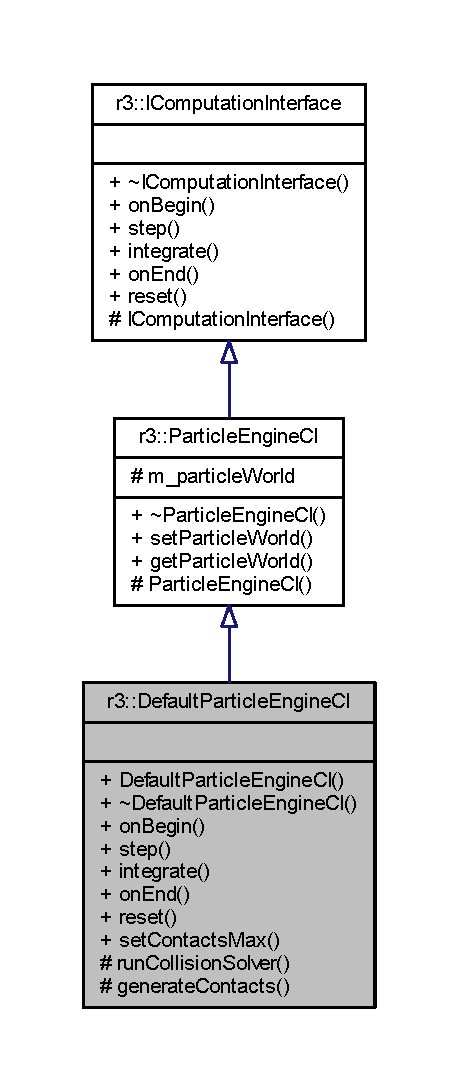
\includegraphics[width=220pt]{classr3_1_1_default_particle_engine_c_i__inherit__graph}
\end{center}
\end{figure}


Collaboration diagram for r3\+:\+:Default\+Particle\+Engine\+CI\+:\nopagebreak
\begin{figure}[H]
\begin{center}
\leavevmode
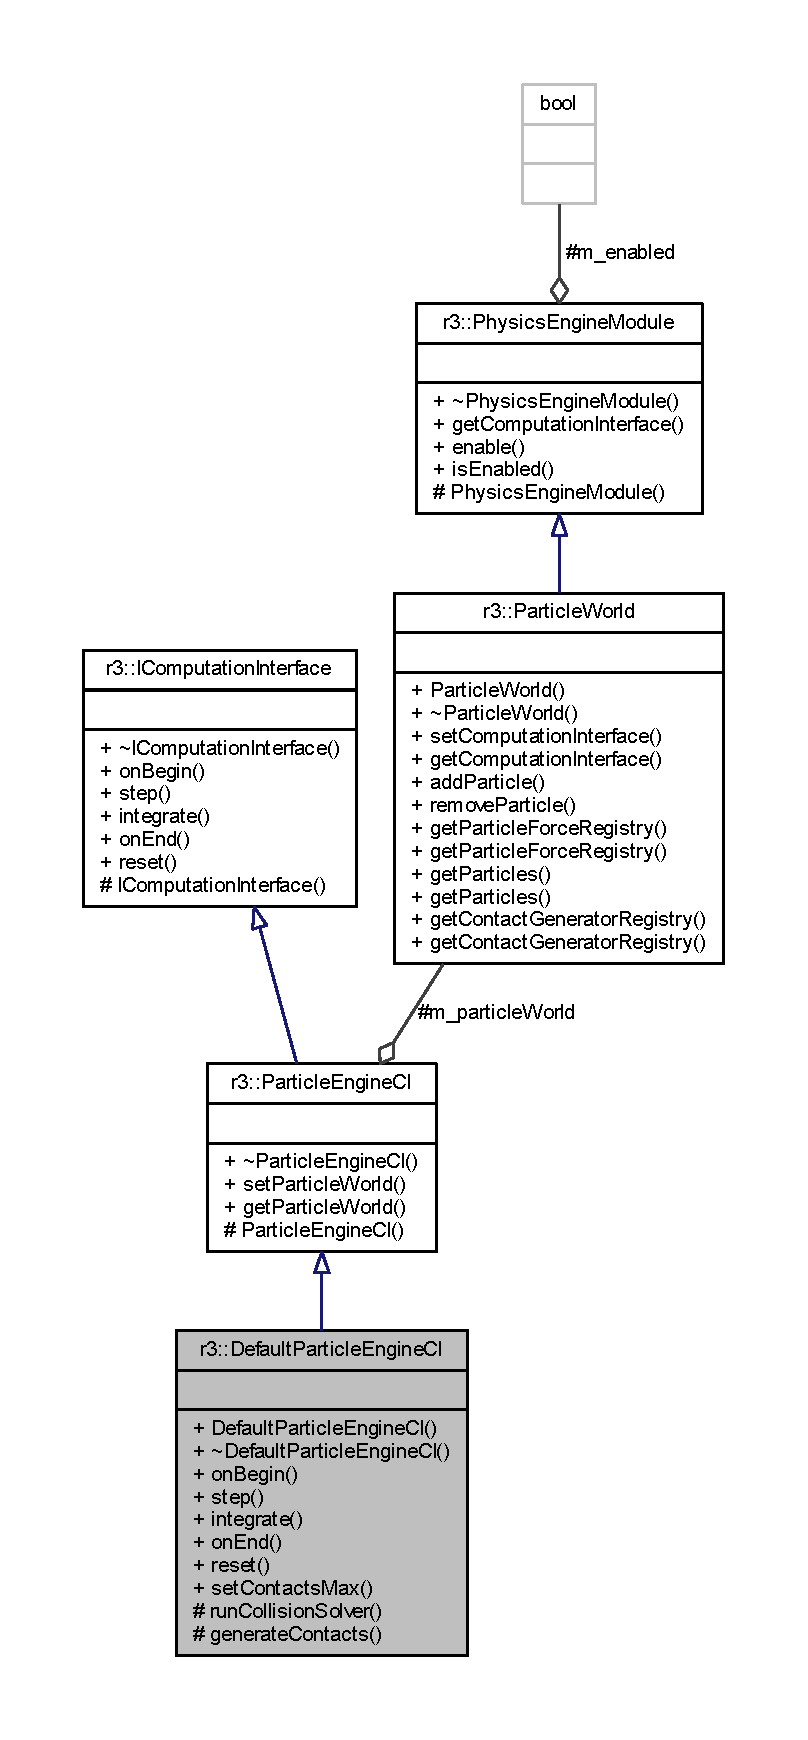
\includegraphics[height=550pt]{classr3_1_1_default_particle_engine_c_i__coll__graph}
\end{center}
\end{figure}
\subsection*{Public Member Functions}
\begin{DoxyCompactItemize}
\item 
\mbox{\hyperlink{classr3_1_1_default_particle_engine_c_i_a5f7619a5dd227d681d5dcbde6e8368eb}{Default\+Particle\+Engine\+CI}} (unsigned contacts\+Max, unsigned iterations=0, \mbox{\hyperlink{classr3_1_1_particle_world}{Particle\+World}} $\ast$particle\+World=nullptr)
\begin{DoxyCompactList}\small\item\em \mbox{\hyperlink{classr3_1_1_default_particle_engine_c_i}{Default\+Particle\+Engine\+CI}} constructor. \end{DoxyCompactList}\item 
\mbox{\hyperlink{classr3_1_1_default_particle_engine_c_i_afb7df43eb7fe45d6bcb15c39e3c30849}{$\sim$\+Default\+Particle\+Engine\+CI}} ()
\item 
void \mbox{\hyperlink{classr3_1_1_default_particle_engine_c_i_aaf2e9ca87bff5e48c8eb59384e9cf180}{on\+Begin}} () override
\begin{DoxyCompactList}\small\item\em Called at the start of a physics step. \end{DoxyCompactList}\item 
void \mbox{\hyperlink{classr3_1_1_default_particle_engine_c_i_a7c58fd00ec521410e1b412e9885ee0d2}{step}} (\mbox{\hyperlink{namespacer3_ab2016b3e3f743fb735afce242f0dc1eb}{real}} time\+Delta) override
\begin{DoxyCompactList}\small\item\em Update particle forces. \end{DoxyCompactList}\item 
void \mbox{\hyperlink{classr3_1_1_default_particle_engine_c_i_a4603707afe6c841a83294a46ea4a1c62}{integrate}} (\mbox{\hyperlink{namespacer3_ab2016b3e3f743fb735afce242f0dc1eb}{real}} time\+Delta) override
\begin{DoxyCompactList}\small\item\em Perform integration and solve collisions. \end{DoxyCompactList}\item 
void \mbox{\hyperlink{classr3_1_1_default_particle_engine_c_i_a6a34c77436d8133560eaa7366c740119}{on\+End}} () override
\begin{DoxyCompactList}\small\item\em Clear force accumulators and reset contact data. \end{DoxyCompactList}\item 
void \mbox{\hyperlink{classr3_1_1_default_particle_engine_c_i_a97757c62b4cb1266da29e2b5625bb9d3}{reset}} () override
\begin{DoxyCompactList}\small\item\em Reset the computation interface. \end{DoxyCompactList}\item 
void \mbox{\hyperlink{classr3_1_1_default_particle_engine_c_i_a7dbb49cbf2f5b028656ea2e14174a3ed}{set\+Contacts\+Max}} (unsigned contacts\+Max)
\begin{DoxyCompactList}\small\item\em Set the maximal number of contacts that the collision solver can use. \end{DoxyCompactList}\end{DoxyCompactItemize}
\subsection*{Protected Member Functions}
\begin{DoxyCompactItemize}
\item 
void \mbox{\hyperlink{classr3_1_1_default_particle_engine_c_i_a19138f7707e948b7e8e05647bcba52fe}{run\+Collision\+Solver}} (\mbox{\hyperlink{namespacer3_ab2016b3e3f743fb735afce242f0dc1eb}{real}} time\+Delta)
\begin{DoxyCompactList}\small\item\em Solve all previously generated particle contacts. \end{DoxyCompactList}\item 
void \mbox{\hyperlink{classr3_1_1_default_particle_engine_c_i_a61aea4f32cc73960915d3c68396bd47e}{generate\+Contacts}} ()
\begin{DoxyCompactList}\small\item\em Generate particle contacts by using all registered particle contact generators. \end{DoxyCompactList}\end{DoxyCompactItemize}
\subsection*{Additional Inherited Members}


\subsection{Detailed Description}
Default implementation of the particle computation interface. 

\subsection{Constructor \& Destructor Documentation}
\mbox{\Hypertarget{classr3_1_1_default_particle_engine_c_i_a5f7619a5dd227d681d5dcbde6e8368eb}\label{classr3_1_1_default_particle_engine_c_i_a5f7619a5dd227d681d5dcbde6e8368eb}} 
\index{r3\+::\+Default\+Particle\+Engine\+CI@{r3\+::\+Default\+Particle\+Engine\+CI}!Default\+Particle\+Engine\+CI@{Default\+Particle\+Engine\+CI}}
\index{Default\+Particle\+Engine\+CI@{Default\+Particle\+Engine\+CI}!r3\+::\+Default\+Particle\+Engine\+CI@{r3\+::\+Default\+Particle\+Engine\+CI}}
\subsubsection{\texorpdfstring{Default\+Particle\+Engine\+C\+I()}{DefaultParticleEngineCI()}}
{\footnotesize\ttfamily r3\+::\+Default\+Particle\+Engine\+C\+I\+::\+Default\+Particle\+Engine\+CI (\begin{DoxyParamCaption}\item[{unsigned}]{contacts\+Max,  }\item[{unsigned}]{iterations = {\ttfamily 0},  }\item[{\mbox{\hyperlink{classr3_1_1_particle_world}{Particle\+World}} $\ast$}]{particle\+World = {\ttfamily nullptr} }\end{DoxyParamCaption})\hspace{0.3cm}{\ttfamily [explicit]}}



\mbox{\hyperlink{classr3_1_1_default_particle_engine_c_i}{Default\+Particle\+Engine\+CI}} constructor. 


\begin{DoxyParams}{Parameters}
{\em contacts\+Max} & Maximal number of contacts, which can exist at the same time. \\
\hline
{\em iterations} & Maximal number of iterations the particle contact generator can use. \\
\hline
{\em particle\+World} & The particle world, which should be used for calculations. \\
\hline
\end{DoxyParams}
\mbox{\Hypertarget{classr3_1_1_default_particle_engine_c_i_afb7df43eb7fe45d6bcb15c39e3c30849}\label{classr3_1_1_default_particle_engine_c_i_afb7df43eb7fe45d6bcb15c39e3c30849}} 
\index{r3\+::\+Default\+Particle\+Engine\+CI@{r3\+::\+Default\+Particle\+Engine\+CI}!````~Default\+Particle\+Engine\+CI@{$\sim$\+Default\+Particle\+Engine\+CI}}
\index{````~Default\+Particle\+Engine\+CI@{$\sim$\+Default\+Particle\+Engine\+CI}!r3\+::\+Default\+Particle\+Engine\+CI@{r3\+::\+Default\+Particle\+Engine\+CI}}
\subsubsection{\texorpdfstring{$\sim$\+Default\+Particle\+Engine\+C\+I()}{~DefaultParticleEngineCI()}}
{\footnotesize\ttfamily r3\+::\+Default\+Particle\+Engine\+C\+I\+::$\sim$\+Default\+Particle\+Engine\+CI (\begin{DoxyParamCaption}{ }\end{DoxyParamCaption})\hspace{0.3cm}{\ttfamily [default]}}



\subsection{Member Function Documentation}
\mbox{\Hypertarget{classr3_1_1_default_particle_engine_c_i_a61aea4f32cc73960915d3c68396bd47e}\label{classr3_1_1_default_particle_engine_c_i_a61aea4f32cc73960915d3c68396bd47e}} 
\index{r3\+::\+Default\+Particle\+Engine\+CI@{r3\+::\+Default\+Particle\+Engine\+CI}!generate\+Contacts@{generate\+Contacts}}
\index{generate\+Contacts@{generate\+Contacts}!r3\+::\+Default\+Particle\+Engine\+CI@{r3\+::\+Default\+Particle\+Engine\+CI}}
\subsubsection{\texorpdfstring{generate\+Contacts()}{generateContacts()}}
{\footnotesize\ttfamily void r3\+::\+Default\+Particle\+Engine\+C\+I\+::generate\+Contacts (\begin{DoxyParamCaption}{ }\end{DoxyParamCaption})\hspace{0.3cm}{\ttfamily [protected]}}



Generate particle contacts by using all registered particle contact generators. 

\mbox{\Hypertarget{classr3_1_1_default_particle_engine_c_i_a4603707afe6c841a83294a46ea4a1c62}\label{classr3_1_1_default_particle_engine_c_i_a4603707afe6c841a83294a46ea4a1c62}} 
\index{r3\+::\+Default\+Particle\+Engine\+CI@{r3\+::\+Default\+Particle\+Engine\+CI}!integrate@{integrate}}
\index{integrate@{integrate}!r3\+::\+Default\+Particle\+Engine\+CI@{r3\+::\+Default\+Particle\+Engine\+CI}}
\subsubsection{\texorpdfstring{integrate()}{integrate()}}
{\footnotesize\ttfamily void r3\+::\+Default\+Particle\+Engine\+C\+I\+::integrate (\begin{DoxyParamCaption}\item[{\mbox{\hyperlink{namespacer3_ab2016b3e3f743fb735afce242f0dc1eb}{real}}}]{time\+Delta }\end{DoxyParamCaption})\hspace{0.3cm}{\ttfamily [override]}, {\ttfamily [virtual]}}



Perform integration and solve collisions. 


\begin{DoxyParams}{Parameters}
{\em time\+Delta} & Time step of this update. \\
\hline
\end{DoxyParams}


Implements \mbox{\hyperlink{classr3_1_1_i_computation_interface_a162250f2b6efbd85460bd0f780d42cff}{r3\+::\+I\+Computation\+Interface}}.

\mbox{\Hypertarget{classr3_1_1_default_particle_engine_c_i_aaf2e9ca87bff5e48c8eb59384e9cf180}\label{classr3_1_1_default_particle_engine_c_i_aaf2e9ca87bff5e48c8eb59384e9cf180}} 
\index{r3\+::\+Default\+Particle\+Engine\+CI@{r3\+::\+Default\+Particle\+Engine\+CI}!on\+Begin@{on\+Begin}}
\index{on\+Begin@{on\+Begin}!r3\+::\+Default\+Particle\+Engine\+CI@{r3\+::\+Default\+Particle\+Engine\+CI}}
\subsubsection{\texorpdfstring{on\+Begin()}{onBegin()}}
{\footnotesize\ttfamily void r3\+::\+Default\+Particle\+Engine\+C\+I\+::on\+Begin (\begin{DoxyParamCaption}{ }\end{DoxyParamCaption})\hspace{0.3cm}{\ttfamily [override]}, {\ttfamily [virtual]}}



Called at the start of a physics step. 



Implements \mbox{\hyperlink{classr3_1_1_i_computation_interface_a430ebc9cb8d4ba064ac6a032ef07edd7}{r3\+::\+I\+Computation\+Interface}}.

\mbox{\Hypertarget{classr3_1_1_default_particle_engine_c_i_a6a34c77436d8133560eaa7366c740119}\label{classr3_1_1_default_particle_engine_c_i_a6a34c77436d8133560eaa7366c740119}} 
\index{r3\+::\+Default\+Particle\+Engine\+CI@{r3\+::\+Default\+Particle\+Engine\+CI}!on\+End@{on\+End}}
\index{on\+End@{on\+End}!r3\+::\+Default\+Particle\+Engine\+CI@{r3\+::\+Default\+Particle\+Engine\+CI}}
\subsubsection{\texorpdfstring{on\+End()}{onEnd()}}
{\footnotesize\ttfamily void r3\+::\+Default\+Particle\+Engine\+C\+I\+::on\+End (\begin{DoxyParamCaption}{ }\end{DoxyParamCaption})\hspace{0.3cm}{\ttfamily [override]}, {\ttfamily [virtual]}}



Clear force accumulators and reset contact data. 



Implements \mbox{\hyperlink{classr3_1_1_i_computation_interface_acae0c5fada7e414c74fe6f5a8f4a6c7d}{r3\+::\+I\+Computation\+Interface}}.

\mbox{\Hypertarget{classr3_1_1_default_particle_engine_c_i_a97757c62b4cb1266da29e2b5625bb9d3}\label{classr3_1_1_default_particle_engine_c_i_a97757c62b4cb1266da29e2b5625bb9d3}} 
\index{r3\+::\+Default\+Particle\+Engine\+CI@{r3\+::\+Default\+Particle\+Engine\+CI}!reset@{reset}}
\index{reset@{reset}!r3\+::\+Default\+Particle\+Engine\+CI@{r3\+::\+Default\+Particle\+Engine\+CI}}
\subsubsection{\texorpdfstring{reset()}{reset()}}
{\footnotesize\ttfamily void r3\+::\+Default\+Particle\+Engine\+C\+I\+::reset (\begin{DoxyParamCaption}{ }\end{DoxyParamCaption})\hspace{0.3cm}{\ttfamily [override]}, {\ttfamily [virtual]}}



Reset the computation interface. 



Implements \mbox{\hyperlink{classr3_1_1_i_computation_interface_a6069989c54ffd4e714788d0968851007}{r3\+::\+I\+Computation\+Interface}}.

\mbox{\Hypertarget{classr3_1_1_default_particle_engine_c_i_a19138f7707e948b7e8e05647bcba52fe}\label{classr3_1_1_default_particle_engine_c_i_a19138f7707e948b7e8e05647bcba52fe}} 
\index{r3\+::\+Default\+Particle\+Engine\+CI@{r3\+::\+Default\+Particle\+Engine\+CI}!run\+Collision\+Solver@{run\+Collision\+Solver}}
\index{run\+Collision\+Solver@{run\+Collision\+Solver}!r3\+::\+Default\+Particle\+Engine\+CI@{r3\+::\+Default\+Particle\+Engine\+CI}}
\subsubsection{\texorpdfstring{run\+Collision\+Solver()}{runCollisionSolver()}}
{\footnotesize\ttfamily void r3\+::\+Default\+Particle\+Engine\+C\+I\+::run\+Collision\+Solver (\begin{DoxyParamCaption}\item[{\mbox{\hyperlink{namespacer3_ab2016b3e3f743fb735afce242f0dc1eb}{real}}}]{time\+Delta }\end{DoxyParamCaption})\hspace{0.3cm}{\ttfamily [protected]}}



Solve all previously generated particle contacts. 

\mbox{\Hypertarget{classr3_1_1_default_particle_engine_c_i_a7dbb49cbf2f5b028656ea2e14174a3ed}\label{classr3_1_1_default_particle_engine_c_i_a7dbb49cbf2f5b028656ea2e14174a3ed}} 
\index{r3\+::\+Default\+Particle\+Engine\+CI@{r3\+::\+Default\+Particle\+Engine\+CI}!set\+Contacts\+Max@{set\+Contacts\+Max}}
\index{set\+Contacts\+Max@{set\+Contacts\+Max}!r3\+::\+Default\+Particle\+Engine\+CI@{r3\+::\+Default\+Particle\+Engine\+CI}}
\subsubsection{\texorpdfstring{set\+Contacts\+Max()}{setContactsMax()}}
{\footnotesize\ttfamily void r3\+::\+Default\+Particle\+Engine\+C\+I\+::set\+Contacts\+Max (\begin{DoxyParamCaption}\item[{unsigned}]{contacts\+Max }\end{DoxyParamCaption})}



Set the maximal number of contacts that the collision solver can use. 


\begin{DoxyParams}{Parameters}
{\em contacts\+Max} & The maximal number of contacts. \\
\hline
\end{DoxyParams}
\mbox{\Hypertarget{classr3_1_1_default_particle_engine_c_i_a7c58fd00ec521410e1b412e9885ee0d2}\label{classr3_1_1_default_particle_engine_c_i_a7c58fd00ec521410e1b412e9885ee0d2}} 
\index{r3\+::\+Default\+Particle\+Engine\+CI@{r3\+::\+Default\+Particle\+Engine\+CI}!step@{step}}
\index{step@{step}!r3\+::\+Default\+Particle\+Engine\+CI@{r3\+::\+Default\+Particle\+Engine\+CI}}
\subsubsection{\texorpdfstring{step()}{step()}}
{\footnotesize\ttfamily void r3\+::\+Default\+Particle\+Engine\+C\+I\+::step (\begin{DoxyParamCaption}\item[{\mbox{\hyperlink{namespacer3_ab2016b3e3f743fb735afce242f0dc1eb}{real}}}]{time\+Delta }\end{DoxyParamCaption})\hspace{0.3cm}{\ttfamily [override]}, {\ttfamily [virtual]}}



Update particle forces. 


\begin{DoxyParams}{Parameters}
{\em time\+Delta} & Time step of this update. \\
\hline
\end{DoxyParams}


Implements \mbox{\hyperlink{classr3_1_1_i_computation_interface_aaa12bcc35005f32a1984b38de97696cb}{r3\+::\+I\+Computation\+Interface}}.



The documentation for this class was generated from the following files\+:\begin{DoxyCompactItemize}
\item 
D\+:/\+Library/\+Documents/\+Job/\+Forschungsmaster/\+Projekte/\+Simulation\+Visualization/\+Rumble3\+D/\+Rumble3\+D/include/\+R3\+D/\+Particle\+Engine/\mbox{\hyperlink{_default_particle_engine_c_i_8h}{Default\+Particle\+Engine\+C\+I.\+h}}\item 
D\+:/\+Library/\+Documents/\+Job/\+Forschungsmaster/\+Projekte/\+Simulation\+Visualization/\+Rumble3\+D/\+Rumble3\+D/src/\+Particle\+Engine/\mbox{\hyperlink{_default_particle_engine_c_i_8cpp}{Default\+Particle\+Engine\+C\+I.\+cpp}}\end{DoxyCompactItemize}

\hypertarget{classr3_1_1_default_rigid_body_engine_c_i}{}\section{r3\+:\+:Default\+Rigid\+Body\+Engine\+CI Class Reference}
\label{classr3_1_1_default_rigid_body_engine_c_i}\index{r3\+::\+Default\+Rigid\+Body\+Engine\+CI@{r3\+::\+Default\+Rigid\+Body\+Engine\+CI}}


Default implementation of the rigid body engine computation interface.  




{\ttfamily \#include $<$Default\+Rigid\+Body\+Engine\+C\+I.\+h$>$}



Inheritance diagram for r3\+:\+:Default\+Rigid\+Body\+Engine\+CI\+:\nopagebreak
\begin{figure}[H]
\begin{center}
\leavevmode
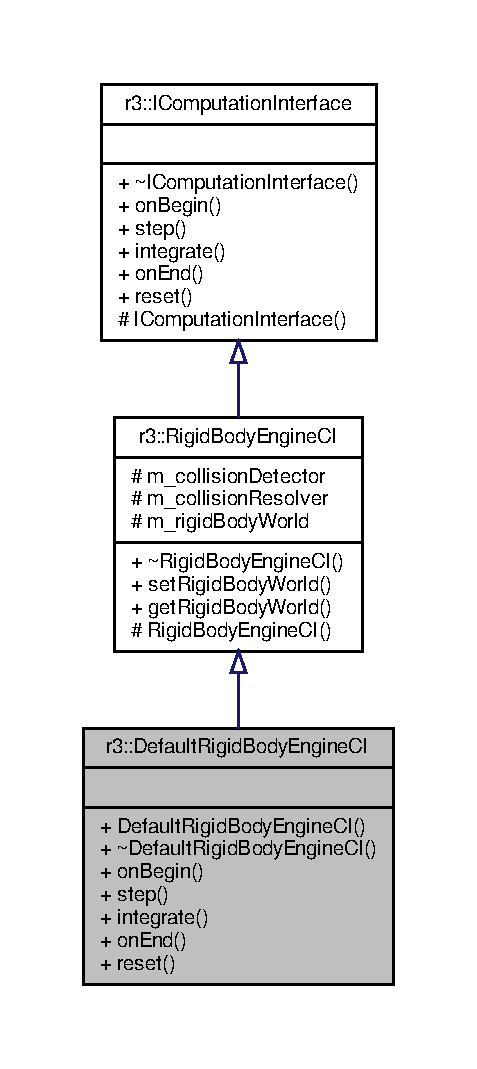
\includegraphics[width=231pt]{classr3_1_1_default_rigid_body_engine_c_i__inherit__graph}
\end{center}
\end{figure}


Collaboration diagram for r3\+:\+:Default\+Rigid\+Body\+Engine\+CI\+:\nopagebreak
\begin{figure}[H]
\begin{center}
\leavevmode
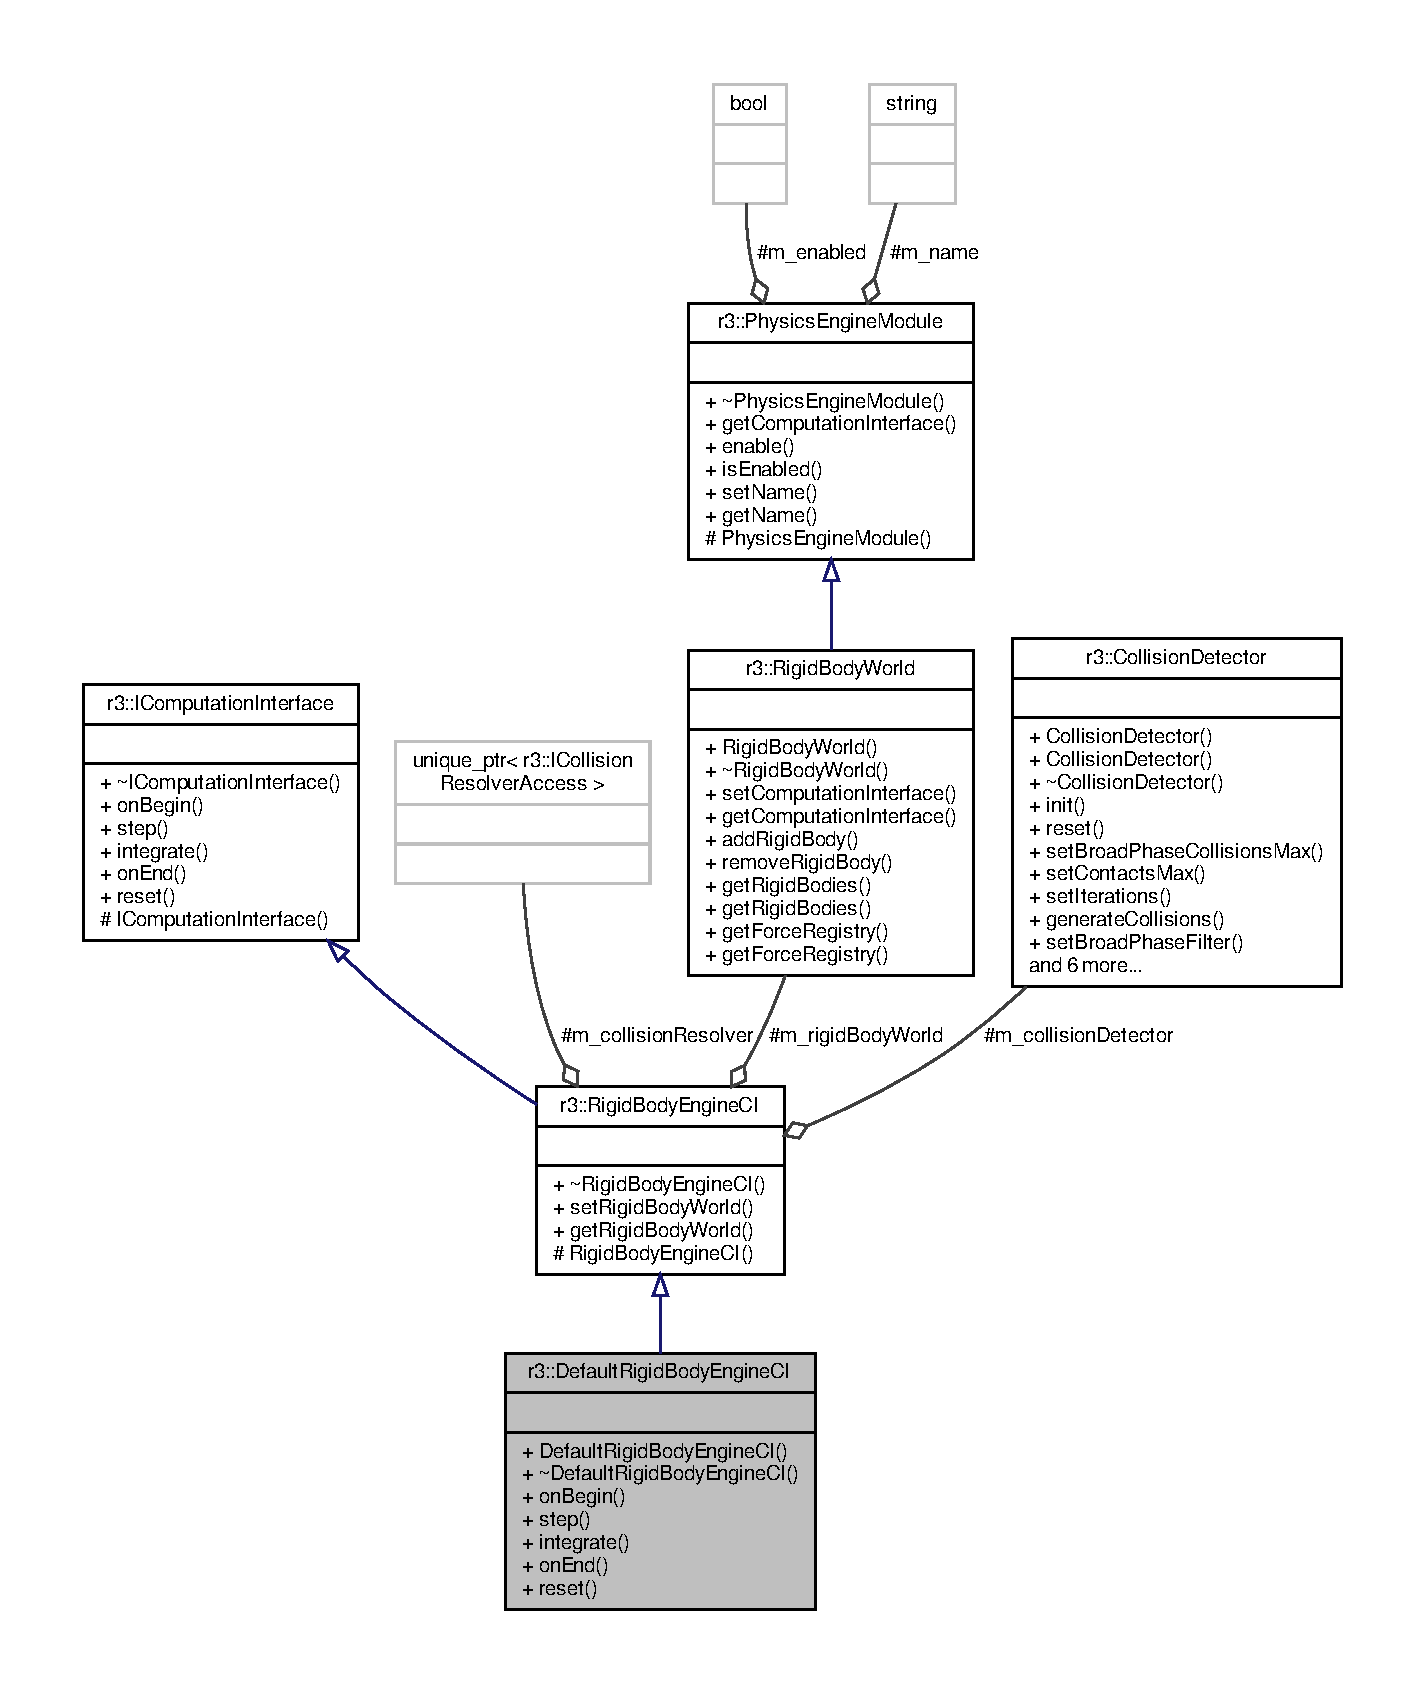
\includegraphics[width=350pt]{classr3_1_1_default_rigid_body_engine_c_i__coll__graph}
\end{center}
\end{figure}
\subsection*{Public Member Functions}
\begin{DoxyCompactItemize}
\item 
\mbox{\hyperlink{classr3_1_1_default_rigid_body_engine_c_i_a277f7da049340a3957fdaf8cb7ee0dfe}{Default\+Rigid\+Body\+Engine\+CI}} ()
\item 
\mbox{\hyperlink{classr3_1_1_default_rigid_body_engine_c_i_af68e19bbae7b792bf57d24a4004295eb}{$\sim$\+Default\+Rigid\+Body\+Engine\+CI}} ()
\item 
void \mbox{\hyperlink{classr3_1_1_default_rigid_body_engine_c_i_a5d9e40ea40845499f01081d21cd9ff64}{on\+Begin}} () override
\begin{DoxyCompactList}\small\item\em Prepare rigid bodies. \end{DoxyCompactList}\item 
void \mbox{\hyperlink{classr3_1_1_default_rigid_body_engine_c_i_ac45ae1d1889c75e6839b865870cbf59c}{step}} (\mbox{\hyperlink{namespacer3_ab2016b3e3f743fb735afce242f0dc1eb}{real}} time\+Delta) override
\begin{DoxyCompactList}\small\item\em Update forces on rigid bodies. \end{DoxyCompactList}\item 
void \mbox{\hyperlink{classr3_1_1_default_rigid_body_engine_c_i_a4b79e7e4bc76eedcad7ef5c4777b9d33}{integrate}} (\mbox{\hyperlink{namespacer3_ab2016b3e3f743fb735afce242f0dc1eb}{real}} time\+Delta) override
\begin{DoxyCompactList}\small\item\em Update positions, rotations and resolve collisions. \end{DoxyCompactList}\item 
void \mbox{\hyperlink{classr3_1_1_default_rigid_body_engine_c_i_ad7746126ebd5aab4cfc352dd9facabb2}{on\+End}} () override
\begin{DoxyCompactList}\small\item\em Clear accumulators. \end{DoxyCompactList}\item 
void \mbox{\hyperlink{classr3_1_1_default_rigid_body_engine_c_i_a06bd27e94b26017e7960e01f6e884e33}{reset}} () override
\begin{DoxyCompactList}\small\item\em Reset the computation interface. \end{DoxyCompactList}\end{DoxyCompactItemize}
\subsection*{Additional Inherited Members}


\subsection{Detailed Description}
Default implementation of the rigid body engine computation interface. 

\subsection{Constructor \& Destructor Documentation}
\mbox{\Hypertarget{classr3_1_1_default_rigid_body_engine_c_i_a277f7da049340a3957fdaf8cb7ee0dfe}\label{classr3_1_1_default_rigid_body_engine_c_i_a277f7da049340a3957fdaf8cb7ee0dfe}} 
\index{r3\+::\+Default\+Rigid\+Body\+Engine\+CI@{r3\+::\+Default\+Rigid\+Body\+Engine\+CI}!Default\+Rigid\+Body\+Engine\+CI@{Default\+Rigid\+Body\+Engine\+CI}}
\index{Default\+Rigid\+Body\+Engine\+CI@{Default\+Rigid\+Body\+Engine\+CI}!r3\+::\+Default\+Rigid\+Body\+Engine\+CI@{r3\+::\+Default\+Rigid\+Body\+Engine\+CI}}
\subsubsection{\texorpdfstring{Default\+Rigid\+Body\+Engine\+C\+I()}{DefaultRigidBodyEngineCI()}}
{\footnotesize\ttfamily r3\+::\+Default\+Rigid\+Body\+Engine\+C\+I\+::\+Default\+Rigid\+Body\+Engine\+CI (\begin{DoxyParamCaption}{ }\end{DoxyParamCaption})\hspace{0.3cm}{\ttfamily [explicit]}}

\mbox{\Hypertarget{classr3_1_1_default_rigid_body_engine_c_i_af68e19bbae7b792bf57d24a4004295eb}\label{classr3_1_1_default_rigid_body_engine_c_i_af68e19bbae7b792bf57d24a4004295eb}} 
\index{r3\+::\+Default\+Rigid\+Body\+Engine\+CI@{r3\+::\+Default\+Rigid\+Body\+Engine\+CI}!````~Default\+Rigid\+Body\+Engine\+CI@{$\sim$\+Default\+Rigid\+Body\+Engine\+CI}}
\index{````~Default\+Rigid\+Body\+Engine\+CI@{$\sim$\+Default\+Rigid\+Body\+Engine\+CI}!r3\+::\+Default\+Rigid\+Body\+Engine\+CI@{r3\+::\+Default\+Rigid\+Body\+Engine\+CI}}
\subsubsection{\texorpdfstring{$\sim$\+Default\+Rigid\+Body\+Engine\+C\+I()}{~DefaultRigidBodyEngineCI()}}
{\footnotesize\ttfamily r3\+::\+Default\+Rigid\+Body\+Engine\+C\+I\+::$\sim$\+Default\+Rigid\+Body\+Engine\+CI (\begin{DoxyParamCaption}{ }\end{DoxyParamCaption})\hspace{0.3cm}{\ttfamily [default]}}



\subsection{Member Function Documentation}
\mbox{\Hypertarget{classr3_1_1_default_rigid_body_engine_c_i_a4b79e7e4bc76eedcad7ef5c4777b9d33}\label{classr3_1_1_default_rigid_body_engine_c_i_a4b79e7e4bc76eedcad7ef5c4777b9d33}} 
\index{r3\+::\+Default\+Rigid\+Body\+Engine\+CI@{r3\+::\+Default\+Rigid\+Body\+Engine\+CI}!integrate@{integrate}}
\index{integrate@{integrate}!r3\+::\+Default\+Rigid\+Body\+Engine\+CI@{r3\+::\+Default\+Rigid\+Body\+Engine\+CI}}
\subsubsection{\texorpdfstring{integrate()}{integrate()}}
{\footnotesize\ttfamily void r3\+::\+Default\+Rigid\+Body\+Engine\+C\+I\+::integrate (\begin{DoxyParamCaption}\item[{\mbox{\hyperlink{namespacer3_ab2016b3e3f743fb735afce242f0dc1eb}{real}}}]{time\+Delta }\end{DoxyParamCaption})\hspace{0.3cm}{\ttfamily [override]}, {\ttfamily [virtual]}}



Update positions, rotations and resolve collisions. 


\begin{DoxyParams}{Parameters}
{\em time\+Delta} & Time step of the simulation update. \\
\hline
\end{DoxyParams}


Implements \mbox{\hyperlink{classr3_1_1_i_computation_interface_a162250f2b6efbd85460bd0f780d42cff}{r3\+::\+I\+Computation\+Interface}}.

\mbox{\Hypertarget{classr3_1_1_default_rigid_body_engine_c_i_a5d9e40ea40845499f01081d21cd9ff64}\label{classr3_1_1_default_rigid_body_engine_c_i_a5d9e40ea40845499f01081d21cd9ff64}} 
\index{r3\+::\+Default\+Rigid\+Body\+Engine\+CI@{r3\+::\+Default\+Rigid\+Body\+Engine\+CI}!on\+Begin@{on\+Begin}}
\index{on\+Begin@{on\+Begin}!r3\+::\+Default\+Rigid\+Body\+Engine\+CI@{r3\+::\+Default\+Rigid\+Body\+Engine\+CI}}
\subsubsection{\texorpdfstring{on\+Begin()}{onBegin()}}
{\footnotesize\ttfamily void r3\+::\+Default\+Rigid\+Body\+Engine\+C\+I\+::on\+Begin (\begin{DoxyParamCaption}{ }\end{DoxyParamCaption})\hspace{0.3cm}{\ttfamily [override]}, {\ttfamily [virtual]}}



Prepare rigid bodies. 



Implements \mbox{\hyperlink{classr3_1_1_i_computation_interface_a430ebc9cb8d4ba064ac6a032ef07edd7}{r3\+::\+I\+Computation\+Interface}}.

\mbox{\Hypertarget{classr3_1_1_default_rigid_body_engine_c_i_ad7746126ebd5aab4cfc352dd9facabb2}\label{classr3_1_1_default_rigid_body_engine_c_i_ad7746126ebd5aab4cfc352dd9facabb2}} 
\index{r3\+::\+Default\+Rigid\+Body\+Engine\+CI@{r3\+::\+Default\+Rigid\+Body\+Engine\+CI}!on\+End@{on\+End}}
\index{on\+End@{on\+End}!r3\+::\+Default\+Rigid\+Body\+Engine\+CI@{r3\+::\+Default\+Rigid\+Body\+Engine\+CI}}
\subsubsection{\texorpdfstring{on\+End()}{onEnd()}}
{\footnotesize\ttfamily void r3\+::\+Default\+Rigid\+Body\+Engine\+C\+I\+::on\+End (\begin{DoxyParamCaption}{ }\end{DoxyParamCaption})\hspace{0.3cm}{\ttfamily [override]}, {\ttfamily [virtual]}}



Clear accumulators. 



Implements \mbox{\hyperlink{classr3_1_1_i_computation_interface_acae0c5fada7e414c74fe6f5a8f4a6c7d}{r3\+::\+I\+Computation\+Interface}}.

\mbox{\Hypertarget{classr3_1_1_default_rigid_body_engine_c_i_a06bd27e94b26017e7960e01f6e884e33}\label{classr3_1_1_default_rigid_body_engine_c_i_a06bd27e94b26017e7960e01f6e884e33}} 
\index{r3\+::\+Default\+Rigid\+Body\+Engine\+CI@{r3\+::\+Default\+Rigid\+Body\+Engine\+CI}!reset@{reset}}
\index{reset@{reset}!r3\+::\+Default\+Rigid\+Body\+Engine\+CI@{r3\+::\+Default\+Rigid\+Body\+Engine\+CI}}
\subsubsection{\texorpdfstring{reset()}{reset()}}
{\footnotesize\ttfamily void r3\+::\+Default\+Rigid\+Body\+Engine\+C\+I\+::reset (\begin{DoxyParamCaption}{ }\end{DoxyParamCaption})\hspace{0.3cm}{\ttfamily [override]}, {\ttfamily [virtual]}}



Reset the computation interface. 



Implements \mbox{\hyperlink{classr3_1_1_i_computation_interface_a6069989c54ffd4e714788d0968851007}{r3\+::\+I\+Computation\+Interface}}.

\mbox{\Hypertarget{classr3_1_1_default_rigid_body_engine_c_i_ac45ae1d1889c75e6839b865870cbf59c}\label{classr3_1_1_default_rigid_body_engine_c_i_ac45ae1d1889c75e6839b865870cbf59c}} 
\index{r3\+::\+Default\+Rigid\+Body\+Engine\+CI@{r3\+::\+Default\+Rigid\+Body\+Engine\+CI}!step@{step}}
\index{step@{step}!r3\+::\+Default\+Rigid\+Body\+Engine\+CI@{r3\+::\+Default\+Rigid\+Body\+Engine\+CI}}
\subsubsection{\texorpdfstring{step()}{step()}}
{\footnotesize\ttfamily void r3\+::\+Default\+Rigid\+Body\+Engine\+C\+I\+::step (\begin{DoxyParamCaption}\item[{\mbox{\hyperlink{namespacer3_ab2016b3e3f743fb735afce242f0dc1eb}{real}}}]{time\+Delta }\end{DoxyParamCaption})\hspace{0.3cm}{\ttfamily [override]}, {\ttfamily [virtual]}}



Update forces on rigid bodies. 


\begin{DoxyParams}{Parameters}
{\em time\+Delta} & Time step of the simulation update. \\
\hline
\end{DoxyParams}


Implements \mbox{\hyperlink{classr3_1_1_i_computation_interface_aaa12bcc35005f32a1984b38de97696cb}{r3\+::\+I\+Computation\+Interface}}.



The documentation for this class was generated from the following files\+:\begin{DoxyCompactItemize}
\item 
D\+:/\+Programming/\+Repositories/\+Game\+Physics/\+Simulation\+Visualization/\+Rumble3\+D/\+Rumble3\+D/include/\+R3\+D/\+Rigid\+Body\+Engine/\mbox{\hyperlink{_default_rigid_body_engine_c_i_8h}{Default\+Rigid\+Body\+Engine\+C\+I.\+h}}\item 
D\+:/\+Programming/\+Repositories/\+Game\+Physics/\+Simulation\+Visualization/\+Rumble3\+D/\+Rumble3\+D/src/\+Rigid\+Body\+Engine/\mbox{\hyperlink{_default_rigid_body_engine_c_i_8cpp}{Default\+Rigid\+Body\+Engine\+C\+I.\+cpp}}\end{DoxyCompactItemize}

\hypertarget{classr3_1_1_directed_force}{}\section{r3\+:\+:Directed\+Force Class Reference}
\label{classr3_1_1_directed_force}\index{r3\+::\+Directed\+Force@{r3\+::\+Directed\+Force}}


A \mbox{\hyperlink{classr3_1_1_directed_force}{Directed\+Force}} is a force generator, which will continually apply a specified force at a specific body point.  




{\ttfamily \#include $<$Directed\+Force.\+h$>$}



Inheritance diagram for r3\+:\+:Directed\+Force\+:\nopagebreak
\begin{figure}[H]
\begin{center}
\leavevmode
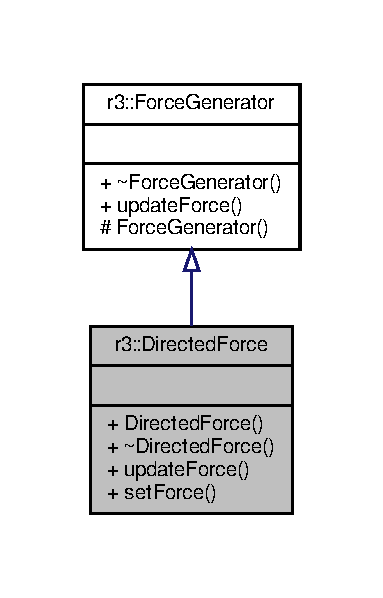
\includegraphics[width=185pt]{classr3_1_1_directed_force__inherit__graph}
\end{center}
\end{figure}


Collaboration diagram for r3\+:\+:Directed\+Force\+:\nopagebreak
\begin{figure}[H]
\begin{center}
\leavevmode
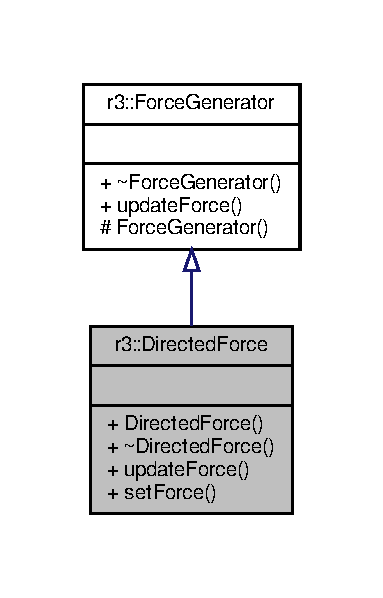
\includegraphics[width=185pt]{classr3_1_1_directed_force__coll__graph}
\end{center}
\end{figure}
\subsection*{Public Member Functions}
\begin{DoxyCompactItemize}
\item 
\mbox{\hyperlink{classr3_1_1_directed_force_a01b61a6ebe0c54f92952d69e3d0cf09e}{Directed\+Force}} (const glm\+::vec3 \&local\+Position, const glm\+::vec3 \&force)
\begin{DoxyCompactList}\small\item\em \mbox{\hyperlink{classr3_1_1_directed_force}{Directed\+Force}} constructor. \end{DoxyCompactList}\item 
\mbox{\hyperlink{classr3_1_1_directed_force_a98aa1b750a187ba18a6fce0c530e397f}{$\sim$\+Directed\+Force}} ()
\item 
void \mbox{\hyperlink{classr3_1_1_directed_force_ac723ddeef767956d16fb9d0a1d706bfd}{update\+Force}} (\mbox{\hyperlink{classr3_1_1_rigid_body}{Rigid\+Body}} $\ast$body, \mbox{\hyperlink{namespacer3_ab2016b3e3f743fb735afce242f0dc1eb}{real}} duration) override
\begin{DoxyCompactList}\small\item\em Apply force to a rigid body over a specific time. \end{DoxyCompactList}\item 
void \mbox{\hyperlink{classr3_1_1_directed_force_a5c25cdaa94e053ffd2614472d2a04c7e}{set\+Force}} (const glm\+::vec3 \&force)
\begin{DoxyCompactList}\small\item\em Set the force, which will act on the body. \end{DoxyCompactList}\end{DoxyCompactItemize}
\subsection*{Additional Inherited Members}


\subsection{Detailed Description}
A \mbox{\hyperlink{classr3_1_1_directed_force}{Directed\+Force}} is a force generator, which will continually apply a specified force at a specific body point. 

\subsection{Constructor \& Destructor Documentation}
\mbox{\Hypertarget{classr3_1_1_directed_force_a01b61a6ebe0c54f92952d69e3d0cf09e}\label{classr3_1_1_directed_force_a01b61a6ebe0c54f92952d69e3d0cf09e}} 
\index{r3\+::\+Directed\+Force@{r3\+::\+Directed\+Force}!Directed\+Force@{Directed\+Force}}
\index{Directed\+Force@{Directed\+Force}!r3\+::\+Directed\+Force@{r3\+::\+Directed\+Force}}
\subsubsection{\texorpdfstring{Directed\+Force()}{DirectedForce()}}
{\footnotesize\ttfamily r3\+::\+Directed\+Force\+::\+Directed\+Force (\begin{DoxyParamCaption}\item[{const glm\+::vec3 \&}]{local\+Position,  }\item[{const glm\+::vec3 \&}]{force }\end{DoxyParamCaption})}



\mbox{\hyperlink{classr3_1_1_directed_force}{Directed\+Force}} constructor. 


\begin{DoxyParams}{Parameters}
{\em local\+Position} & Attack point of the force. \\
\hline
{\em force} & The force, which will act on the body. \\
\hline
\end{DoxyParams}
\mbox{\Hypertarget{classr3_1_1_directed_force_a98aa1b750a187ba18a6fce0c530e397f}\label{classr3_1_1_directed_force_a98aa1b750a187ba18a6fce0c530e397f}} 
\index{r3\+::\+Directed\+Force@{r3\+::\+Directed\+Force}!````~Directed\+Force@{$\sim$\+Directed\+Force}}
\index{````~Directed\+Force@{$\sim$\+Directed\+Force}!r3\+::\+Directed\+Force@{r3\+::\+Directed\+Force}}
\subsubsection{\texorpdfstring{$\sim$\+Directed\+Force()}{~DirectedForce()}}
{\footnotesize\ttfamily r3\+::\+Directed\+Force\+::$\sim$\+Directed\+Force (\begin{DoxyParamCaption}{ }\end{DoxyParamCaption})\hspace{0.3cm}{\ttfamily [default]}}



\subsection{Member Function Documentation}
\mbox{\Hypertarget{classr3_1_1_directed_force_a5c25cdaa94e053ffd2614472d2a04c7e}\label{classr3_1_1_directed_force_a5c25cdaa94e053ffd2614472d2a04c7e}} 
\index{r3\+::\+Directed\+Force@{r3\+::\+Directed\+Force}!set\+Force@{set\+Force}}
\index{set\+Force@{set\+Force}!r3\+::\+Directed\+Force@{r3\+::\+Directed\+Force}}
\subsubsection{\texorpdfstring{set\+Force()}{setForce()}}
{\footnotesize\ttfamily void r3\+::\+Directed\+Force\+::set\+Force (\begin{DoxyParamCaption}\item[{const glm\+::vec3 \&}]{force }\end{DoxyParamCaption})}



Set the force, which will act on the body. 


\begin{DoxyParams}{Parameters}
{\em force} & The new force. \\
\hline
\end{DoxyParams}
\mbox{\Hypertarget{classr3_1_1_directed_force_ac723ddeef767956d16fb9d0a1d706bfd}\label{classr3_1_1_directed_force_ac723ddeef767956d16fb9d0a1d706bfd}} 
\index{r3\+::\+Directed\+Force@{r3\+::\+Directed\+Force}!update\+Force@{update\+Force}}
\index{update\+Force@{update\+Force}!r3\+::\+Directed\+Force@{r3\+::\+Directed\+Force}}
\subsubsection{\texorpdfstring{update\+Force()}{updateForce()}}
{\footnotesize\ttfamily void r3\+::\+Directed\+Force\+::update\+Force (\begin{DoxyParamCaption}\item[{\mbox{\hyperlink{classr3_1_1_rigid_body}{Rigid\+Body}} $\ast$}]{body,  }\item[{\mbox{\hyperlink{namespacer3_ab2016b3e3f743fb735afce242f0dc1eb}{real}}}]{duration }\end{DoxyParamCaption})\hspace{0.3cm}{\ttfamily [override]}, {\ttfamily [virtual]}}



Apply force to a rigid body over a specific time. 


\begin{DoxyParams}{Parameters}
{\em body} & The rigid body on which to apply force. \\
\hline
{\em duration} & The duration over which the force acts. \\
\hline
\end{DoxyParams}
\begin{DoxyRefDesc}{Todo}
\item[\mbox{\hyperlink{todo__todo000016}{Todo}}]\+: add force at body point doesn\textquotesingle{}t create rotational forces. \end{DoxyRefDesc}


Implements \mbox{\hyperlink{classr3_1_1_force_generator_a69bebbde8cef792d6636af50037af2aa}{r3\+::\+Force\+Generator}}.



The documentation for this class was generated from the following files\+:\begin{DoxyCompactItemize}
\item 
D\+:/\+Library/\+Documents/\+Job/\+Forschungsmaster/\+Projekte/\+Simulation\+Visualization/\+Rumble3\+D/\+Rumble3\+D/include/\+R3\+D/\+Rigid\+Body\+Engine/\mbox{\hyperlink{_directed_force_8h}{Directed\+Force.\+h}}\item 
D\+:/\+Library/\+Documents/\+Job/\+Forschungsmaster/\+Projekte/\+Simulation\+Visualization/\+Rumble3\+D/\+Rumble3\+D/src/\+Rigid\+Body\+Engine/\mbox{\hyperlink{_directed_force_8cpp}{Directed\+Force.\+cpp}}\end{DoxyCompactItemize}

\hypertarget{classr3_1_1_fixed_size_container}{}\section{r3\+:\+:Fixed\+Size\+Container$<$ Element\+\_\+\+Type, Container\+\_\+\+Type $>$ Class Template Reference}
\label{classr3_1_1_fixed_size_container}\index{r3\+::\+Fixed\+Size\+Container$<$ Element\+\_\+\+Type, Container\+\_\+\+Type $>$@{r3\+::\+Fixed\+Size\+Container$<$ Element\+\_\+\+Type, Container\+\_\+\+Type $>$}}


Template class for a container, which can be resized, with random access (dependent on Container\+\_\+\+Type) and can be filled similar to a stack. Its size in memory will stay the same at all times. Elements can not be erased from it.  




{\ttfamily \#include $<$Fixed\+Size\+Container.\+h$>$}



Inheritance diagram for r3\+:\+:Fixed\+Size\+Container$<$ Element\+\_\+\+Type, Container\+\_\+\+Type $>$\+:\nopagebreak
\begin{figure}[H]
\begin{center}
\leavevmode
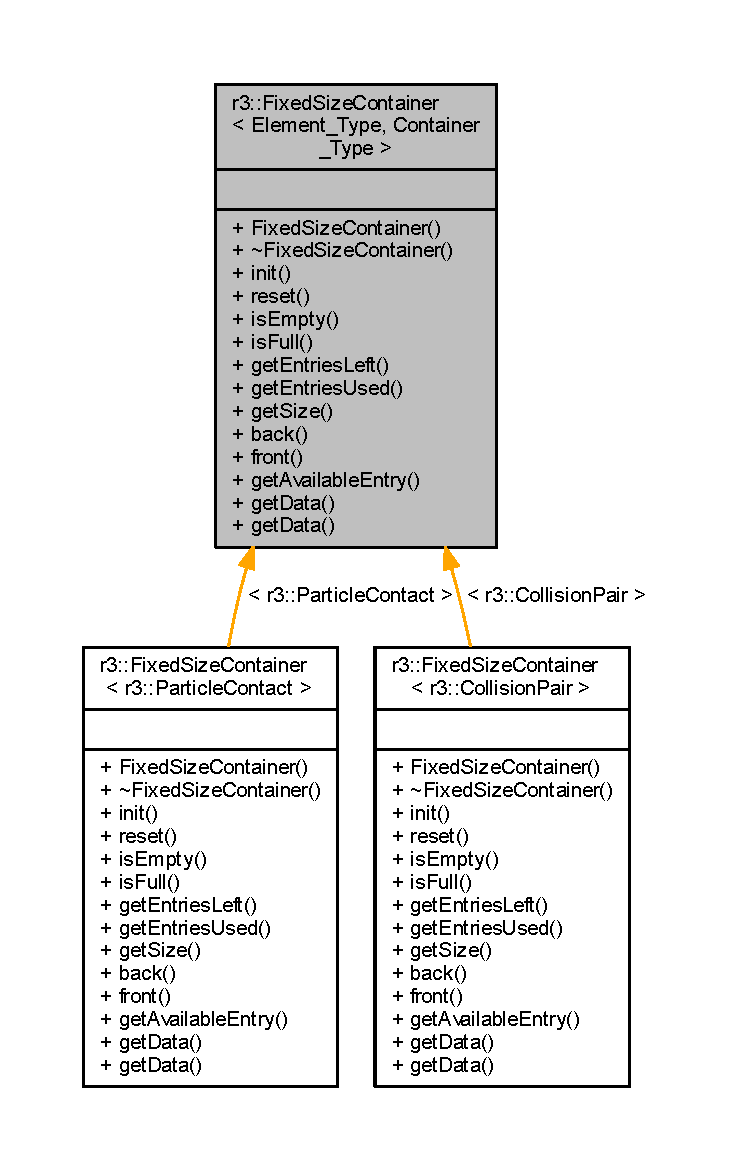
\includegraphics[height=550pt]{classr3_1_1_fixed_size_container__inherit__graph}
\end{center}
\end{figure}


Collaboration diagram for r3\+:\+:Fixed\+Size\+Container$<$ Element\+\_\+\+Type, Container\+\_\+\+Type $>$\+:\nopagebreak
\begin{figure}[H]
\begin{center}
\leavevmode
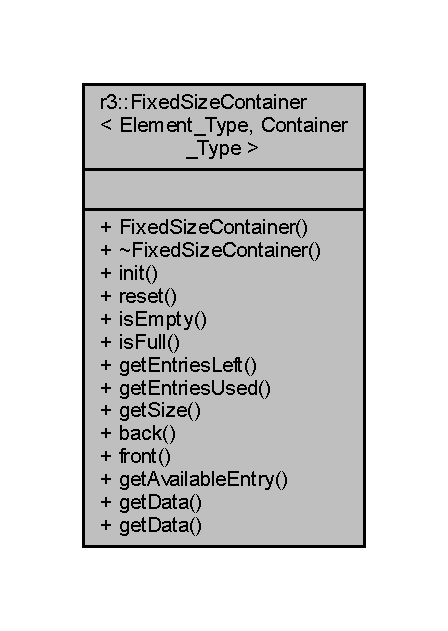
\includegraphics[width=215pt]{classr3_1_1_fixed_size_container__coll__graph}
\end{center}
\end{figure}
\subsection*{Public Member Functions}
\begin{DoxyCompactItemize}
\item 
\mbox{\hyperlink{classr3_1_1_fixed_size_container_a9396266faf0a5d5d75ea50f0d74d5267}{Fixed\+Size\+Container}} (int size)
\begin{DoxyCompactList}\small\item\em \mbox{\hyperlink{classr3_1_1_fixed_size_container}{Fixed\+Size\+Container}} constructor. \end{DoxyCompactList}\item 
\mbox{\hyperlink{classr3_1_1_fixed_size_container_af235a796be8de5a9e96c788b676b59fa}{$\sim$\+Fixed\+Size\+Container}} ()
\item 
void \mbox{\hyperlink{classr3_1_1_fixed_size_container_a75dddd29ba901e97ba6133a6c388b357}{init}} (int size)
\begin{DoxyCompactList}\small\item\em Initialize the container size. This will reset the container. \end{DoxyCompactList}\item 
void \mbox{\hyperlink{classr3_1_1_fixed_size_container_a56aa3725cacf135fc1eacddbf424c868}{reset}} ()
\begin{DoxyCompactList}\small\item\em Reset the number of used entries. \end{DoxyCompactList}\item 
bool \mbox{\hyperlink{classr3_1_1_fixed_size_container_adde8deee5146abd862ef32e1ac3bb879}{is\+Empty}} () const
\begin{DoxyCompactList}\small\item\em Check if no entries are in use. \end{DoxyCompactList}\item 
bool \mbox{\hyperlink{classr3_1_1_fixed_size_container_ae3beb2a45a67d3bd4f6cb32f39805889}{is\+Full}} () const
\begin{DoxyCompactList}\small\item\em Check if the maximal number of usable entries has been reached. \end{DoxyCompactList}\item 
int \mbox{\hyperlink{classr3_1_1_fixed_size_container_a5d21f93fcf7117df372d321c0d9102fa}{get\+Entries\+Left}} () const
\begin{DoxyCompactList}\small\item\em Get the number of elements, which can still fit in the container. \end{DoxyCompactList}\item 
int \mbox{\hyperlink{classr3_1_1_fixed_size_container_a4ec349530e78e78244f739139ed58b49}{get\+Entries\+Used}} () const
\begin{DoxyCompactList}\small\item\em Get the number of elements, which are already stored in the container. \end{DoxyCompactList}\item 
int \mbox{\hyperlink{classr3_1_1_fixed_size_container_a984b90ac15df32a41011e665e3059e17}{get\+Size}} () const
\begin{DoxyCompactList}\small\item\em Get the maximal number of elements, which can fit in this container. \end{DoxyCompactList}\item 
Element\+\_\+\+Type $\ast$ \mbox{\hyperlink{classr3_1_1_fixed_size_container_a6e849d08e5ad5a1a0ef6207f8b36b22e}{back}} ()
\begin{DoxyCompactList}\small\item\em Get the last element. \end{DoxyCompactList}\item 
Element\+\_\+\+Type $\ast$ \mbox{\hyperlink{classr3_1_1_fixed_size_container_ae60eda032ed2276552c7df4fc6da4640}{front}} ()
\begin{DoxyCompactList}\small\item\em Get the first element. \end{DoxyCompactList}\item 
Element\+\_\+\+Type $\ast$ \mbox{\hyperlink{classr3_1_1_fixed_size_container_a7903fc6d43600195b97218aead60a99a}{get\+Available\+Entry}} ()
\begin{DoxyCompactList}\small\item\em Get the next available element. This automatically use the entry. \end{DoxyCompactList}\item 
Container\+\_\+\+Type \& \mbox{\hyperlink{classr3_1_1_fixed_size_container_adbf383734c597677d4221278000886a3}{get\+Data}} ()
\begin{DoxyCompactList}\small\item\em Get the internal container. \end{DoxyCompactList}\item 
const Container\+\_\+\+Type \& \mbox{\hyperlink{classr3_1_1_fixed_size_container_acd837bc4730c98aa4346819726620842}{get\+Data}} () const
\begin{DoxyCompactList}\small\item\em Get the internal container. \end{DoxyCompactList}\end{DoxyCompactItemize}


\subsection{Detailed Description}
\subsubsection*{template$<$class Element\+\_\+\+Type, class Container\+\_\+\+Type = std\+::vector$<$\+Element\+\_\+\+Type$>$$>$\newline
class r3\+::\+Fixed\+Size\+Container$<$ Element\+\_\+\+Type, Container\+\_\+\+Type $>$}

Template class for a container, which can be resized, with random access (dependent on Container\+\_\+\+Type) and can be filled similar to a stack. Its size in memory will stay the same at all times. Elements can not be erased from it. 


\begin{DoxyTemplParams}{Template Parameters}
{\em Element\+\_\+\+Type} & Type of the elements, saved in this container. \\
\hline
{\em Container\+\_\+\+Type} & Container type used for storing elements. Needs to have a \char`\"{}void resize(unsigned)\char`\"{} function and must be able to store elements of type Element\+\_\+\+Type \\
\hline
\end{DoxyTemplParams}


\subsection{Constructor \& Destructor Documentation}
\mbox{\Hypertarget{classr3_1_1_fixed_size_container_a9396266faf0a5d5d75ea50f0d74d5267}\label{classr3_1_1_fixed_size_container_a9396266faf0a5d5d75ea50f0d74d5267}} 
\index{r3\+::\+Fixed\+Size\+Container@{r3\+::\+Fixed\+Size\+Container}!Fixed\+Size\+Container@{Fixed\+Size\+Container}}
\index{Fixed\+Size\+Container@{Fixed\+Size\+Container}!r3\+::\+Fixed\+Size\+Container@{r3\+::\+Fixed\+Size\+Container}}
\subsubsection{\texorpdfstring{Fixed\+Size\+Container()}{FixedSizeContainer()}}
{\footnotesize\ttfamily template$<$class Element\+\_\+\+Type , class Container\+\_\+\+Type $>$ \\
\mbox{\hyperlink{classr3_1_1_fixed_size_container}{r3\+::\+Fixed\+Size\+Container}}$<$ Element\+\_\+\+Type, Container\+\_\+\+Type $>$\+::\mbox{\hyperlink{classr3_1_1_fixed_size_container}{Fixed\+Size\+Container}} (\begin{DoxyParamCaption}\item[{int}]{size }\end{DoxyParamCaption})\hspace{0.3cm}{\ttfamily [explicit]}}



\mbox{\hyperlink{classr3_1_1_fixed_size_container}{Fixed\+Size\+Container}} constructor. 

\mbox{\Hypertarget{classr3_1_1_fixed_size_container_af235a796be8de5a9e96c788b676b59fa}\label{classr3_1_1_fixed_size_container_af235a796be8de5a9e96c788b676b59fa}} 
\index{r3\+::\+Fixed\+Size\+Container@{r3\+::\+Fixed\+Size\+Container}!````~Fixed\+Size\+Container@{$\sim$\+Fixed\+Size\+Container}}
\index{````~Fixed\+Size\+Container@{$\sim$\+Fixed\+Size\+Container}!r3\+::\+Fixed\+Size\+Container@{r3\+::\+Fixed\+Size\+Container}}
\subsubsection{\texorpdfstring{$\sim$\+Fixed\+Size\+Container()}{~FixedSizeContainer()}}
{\footnotesize\ttfamily template$<$class Element\+\_\+\+Type , class Container\+\_\+\+Type $>$ \\
\mbox{\hyperlink{classr3_1_1_fixed_size_container}{r3\+::\+Fixed\+Size\+Container}}$<$ Element\+\_\+\+Type, Container\+\_\+\+Type $>$\+::$\sim$\mbox{\hyperlink{classr3_1_1_fixed_size_container}{Fixed\+Size\+Container}} (\begin{DoxyParamCaption}{ }\end{DoxyParamCaption})\hspace{0.3cm}{\ttfamily [default]}}



\subsection{Member Function Documentation}
\mbox{\Hypertarget{classr3_1_1_fixed_size_container_a6e849d08e5ad5a1a0ef6207f8b36b22e}\label{classr3_1_1_fixed_size_container_a6e849d08e5ad5a1a0ef6207f8b36b22e}} 
\index{r3\+::\+Fixed\+Size\+Container@{r3\+::\+Fixed\+Size\+Container}!back@{back}}
\index{back@{back}!r3\+::\+Fixed\+Size\+Container@{r3\+::\+Fixed\+Size\+Container}}
\subsubsection{\texorpdfstring{back()}{back()}}
{\footnotesize\ttfamily template$<$class Element\+\_\+\+Type , class Container\+\_\+\+Type $>$ \\
Element\+\_\+\+Type $\ast$ \mbox{\hyperlink{classr3_1_1_fixed_size_container}{r3\+::\+Fixed\+Size\+Container}}$<$ Element\+\_\+\+Type, Container\+\_\+\+Type $>$\+::back (\begin{DoxyParamCaption}{ }\end{DoxyParamCaption})}



Get the last element. 

\mbox{\Hypertarget{classr3_1_1_fixed_size_container_ae60eda032ed2276552c7df4fc6da4640}\label{classr3_1_1_fixed_size_container_ae60eda032ed2276552c7df4fc6da4640}} 
\index{r3\+::\+Fixed\+Size\+Container@{r3\+::\+Fixed\+Size\+Container}!front@{front}}
\index{front@{front}!r3\+::\+Fixed\+Size\+Container@{r3\+::\+Fixed\+Size\+Container}}
\subsubsection{\texorpdfstring{front()}{front()}}
{\footnotesize\ttfamily template$<$class Element\+\_\+\+Type , class Container\+\_\+\+Type $>$ \\
Element\+\_\+\+Type $\ast$ \mbox{\hyperlink{classr3_1_1_fixed_size_container}{r3\+::\+Fixed\+Size\+Container}}$<$ Element\+\_\+\+Type, Container\+\_\+\+Type $>$\+::front (\begin{DoxyParamCaption}{ }\end{DoxyParamCaption})}



Get the first element. 

\mbox{\Hypertarget{classr3_1_1_fixed_size_container_a7903fc6d43600195b97218aead60a99a}\label{classr3_1_1_fixed_size_container_a7903fc6d43600195b97218aead60a99a}} 
\index{r3\+::\+Fixed\+Size\+Container@{r3\+::\+Fixed\+Size\+Container}!get\+Available\+Entry@{get\+Available\+Entry}}
\index{get\+Available\+Entry@{get\+Available\+Entry}!r3\+::\+Fixed\+Size\+Container@{r3\+::\+Fixed\+Size\+Container}}
\subsubsection{\texorpdfstring{get\+Available\+Entry()}{getAvailableEntry()}}
{\footnotesize\ttfamily template$<$class Element\+\_\+\+Type , class Container\+\_\+\+Type $>$ \\
Element\+\_\+\+Type $\ast$ \mbox{\hyperlink{classr3_1_1_fixed_size_container}{r3\+::\+Fixed\+Size\+Container}}$<$ Element\+\_\+\+Type, Container\+\_\+\+Type $>$\+::get\+Available\+Entry (\begin{DoxyParamCaption}{ }\end{DoxyParamCaption})}



Get the next available element. This automatically use the entry. 

\begin{DoxyReturn}{Returns}
A free element if there are free entries left, nullptr otherwise. 
\end{DoxyReturn}
\mbox{\Hypertarget{classr3_1_1_fixed_size_container_adbf383734c597677d4221278000886a3}\label{classr3_1_1_fixed_size_container_adbf383734c597677d4221278000886a3}} 
\index{r3\+::\+Fixed\+Size\+Container@{r3\+::\+Fixed\+Size\+Container}!get\+Data@{get\+Data}}
\index{get\+Data@{get\+Data}!r3\+::\+Fixed\+Size\+Container@{r3\+::\+Fixed\+Size\+Container}}
\subsubsection{\texorpdfstring{get\+Data()}{getData()}\hspace{0.1cm}{\footnotesize\ttfamily [1/2]}}
{\footnotesize\ttfamily template$<$class Element\+\_\+\+Type , class Container\+\_\+\+Type $>$ \\
Container\+\_\+\+Type \& \mbox{\hyperlink{classr3_1_1_fixed_size_container}{r3\+::\+Fixed\+Size\+Container}}$<$ Element\+\_\+\+Type, Container\+\_\+\+Type $>$\+::get\+Data (\begin{DoxyParamCaption}{ }\end{DoxyParamCaption})}



Get the internal container. 

\begin{DoxyReturn}{Returns}
All data. Only the first m\+\_\+entries\+Used entries are valid! 
\end{DoxyReturn}
\mbox{\Hypertarget{classr3_1_1_fixed_size_container_acd837bc4730c98aa4346819726620842}\label{classr3_1_1_fixed_size_container_acd837bc4730c98aa4346819726620842}} 
\index{r3\+::\+Fixed\+Size\+Container@{r3\+::\+Fixed\+Size\+Container}!get\+Data@{get\+Data}}
\index{get\+Data@{get\+Data}!r3\+::\+Fixed\+Size\+Container@{r3\+::\+Fixed\+Size\+Container}}
\subsubsection{\texorpdfstring{get\+Data()}{getData()}\hspace{0.1cm}{\footnotesize\ttfamily [2/2]}}
{\footnotesize\ttfamily template$<$class Element\+\_\+\+Type , class Container\+\_\+\+Type $>$ \\
const Container\+\_\+\+Type \& \mbox{\hyperlink{classr3_1_1_fixed_size_container}{r3\+::\+Fixed\+Size\+Container}}$<$ Element\+\_\+\+Type, Container\+\_\+\+Type $>$\+::get\+Data (\begin{DoxyParamCaption}{ }\end{DoxyParamCaption}) const}



Get the internal container. 

\begin{DoxyReturn}{Returns}
All data. Only the first m\+\_\+entries\+Used entries are valid! 
\end{DoxyReturn}
\mbox{\Hypertarget{classr3_1_1_fixed_size_container_a5d21f93fcf7117df372d321c0d9102fa}\label{classr3_1_1_fixed_size_container_a5d21f93fcf7117df372d321c0d9102fa}} 
\index{r3\+::\+Fixed\+Size\+Container@{r3\+::\+Fixed\+Size\+Container}!get\+Entries\+Left@{get\+Entries\+Left}}
\index{get\+Entries\+Left@{get\+Entries\+Left}!r3\+::\+Fixed\+Size\+Container@{r3\+::\+Fixed\+Size\+Container}}
\subsubsection{\texorpdfstring{get\+Entries\+Left()}{getEntriesLeft()}}
{\footnotesize\ttfamily template$<$class Element\+\_\+\+Type , class Container\+\_\+\+Type $>$ \\
int \mbox{\hyperlink{classr3_1_1_fixed_size_container}{r3\+::\+Fixed\+Size\+Container}}$<$ Element\+\_\+\+Type, Container\+\_\+\+Type $>$\+::get\+Entries\+Left (\begin{DoxyParamCaption}{ }\end{DoxyParamCaption}) const}



Get the number of elements, which can still fit in the container. 

\begin{DoxyReturn}{Returns}
The count of free entries. 
\end{DoxyReturn}
\mbox{\Hypertarget{classr3_1_1_fixed_size_container_a4ec349530e78e78244f739139ed58b49}\label{classr3_1_1_fixed_size_container_a4ec349530e78e78244f739139ed58b49}} 
\index{r3\+::\+Fixed\+Size\+Container@{r3\+::\+Fixed\+Size\+Container}!get\+Entries\+Used@{get\+Entries\+Used}}
\index{get\+Entries\+Used@{get\+Entries\+Used}!r3\+::\+Fixed\+Size\+Container@{r3\+::\+Fixed\+Size\+Container}}
\subsubsection{\texorpdfstring{get\+Entries\+Used()}{getEntriesUsed()}}
{\footnotesize\ttfamily template$<$class Element\+\_\+\+Type , class Container\+\_\+\+Type $>$ \\
int \mbox{\hyperlink{classr3_1_1_fixed_size_container}{r3\+::\+Fixed\+Size\+Container}}$<$ Element\+\_\+\+Type, Container\+\_\+\+Type $>$\+::get\+Entries\+Used (\begin{DoxyParamCaption}{ }\end{DoxyParamCaption}) const}



Get the number of elements, which are already stored in the container. 

\begin{DoxyReturn}{Returns}
The number of used entries. 
\end{DoxyReturn}
\mbox{\Hypertarget{classr3_1_1_fixed_size_container_a984b90ac15df32a41011e665e3059e17}\label{classr3_1_1_fixed_size_container_a984b90ac15df32a41011e665e3059e17}} 
\index{r3\+::\+Fixed\+Size\+Container@{r3\+::\+Fixed\+Size\+Container}!get\+Size@{get\+Size}}
\index{get\+Size@{get\+Size}!r3\+::\+Fixed\+Size\+Container@{r3\+::\+Fixed\+Size\+Container}}
\subsubsection{\texorpdfstring{get\+Size()}{getSize()}}
{\footnotesize\ttfamily template$<$class Element\+\_\+\+Type , class Container\+\_\+\+Type $>$ \\
int \mbox{\hyperlink{classr3_1_1_fixed_size_container}{r3\+::\+Fixed\+Size\+Container}}$<$ Element\+\_\+\+Type, Container\+\_\+\+Type $>$\+::get\+Size (\begin{DoxyParamCaption}{ }\end{DoxyParamCaption}) const}



Get the maximal number of elements, which can fit in this container. 

\begin{DoxyReturn}{Returns}
The maximal number of elements. 
\end{DoxyReturn}
\mbox{\Hypertarget{classr3_1_1_fixed_size_container_a75dddd29ba901e97ba6133a6c388b357}\label{classr3_1_1_fixed_size_container_a75dddd29ba901e97ba6133a6c388b357}} 
\index{r3\+::\+Fixed\+Size\+Container@{r3\+::\+Fixed\+Size\+Container}!init@{init}}
\index{init@{init}!r3\+::\+Fixed\+Size\+Container@{r3\+::\+Fixed\+Size\+Container}}
\subsubsection{\texorpdfstring{init()}{init()}}
{\footnotesize\ttfamily template$<$class Element\+\_\+\+Type , class Container\+\_\+\+Type $>$ \\
void \mbox{\hyperlink{classr3_1_1_fixed_size_container}{r3\+::\+Fixed\+Size\+Container}}$<$ Element\+\_\+\+Type, Container\+\_\+\+Type $>$\+::init (\begin{DoxyParamCaption}\item[{int}]{size }\end{DoxyParamCaption})}



Initialize the container size. This will reset the container. 


\begin{DoxyParams}{Parameters}
{\em size} & The new size of the container. \\
\hline
\end{DoxyParams}
\mbox{\Hypertarget{classr3_1_1_fixed_size_container_adde8deee5146abd862ef32e1ac3bb879}\label{classr3_1_1_fixed_size_container_adde8deee5146abd862ef32e1ac3bb879}} 
\index{r3\+::\+Fixed\+Size\+Container@{r3\+::\+Fixed\+Size\+Container}!is\+Empty@{is\+Empty}}
\index{is\+Empty@{is\+Empty}!r3\+::\+Fixed\+Size\+Container@{r3\+::\+Fixed\+Size\+Container}}
\subsubsection{\texorpdfstring{is\+Empty()}{isEmpty()}}
{\footnotesize\ttfamily template$<$class Element\+\_\+\+Type , class Container\+\_\+\+Type $>$ \\
bool \mbox{\hyperlink{classr3_1_1_fixed_size_container}{r3\+::\+Fixed\+Size\+Container}}$<$ Element\+\_\+\+Type, Container\+\_\+\+Type $>$\+::is\+Empty (\begin{DoxyParamCaption}{ }\end{DoxyParamCaption}) const}



Check if no entries are in use. 

\begin{DoxyReturn}{Returns}
True if no entries are in use, false otherwise. 
\end{DoxyReturn}
\mbox{\Hypertarget{classr3_1_1_fixed_size_container_ae3beb2a45a67d3bd4f6cb32f39805889}\label{classr3_1_1_fixed_size_container_ae3beb2a45a67d3bd4f6cb32f39805889}} 
\index{r3\+::\+Fixed\+Size\+Container@{r3\+::\+Fixed\+Size\+Container}!is\+Full@{is\+Full}}
\index{is\+Full@{is\+Full}!r3\+::\+Fixed\+Size\+Container@{r3\+::\+Fixed\+Size\+Container}}
\subsubsection{\texorpdfstring{is\+Full()}{isFull()}}
{\footnotesize\ttfamily template$<$class Element\+\_\+\+Type , class Container\+\_\+\+Type $>$ \\
bool \mbox{\hyperlink{classr3_1_1_fixed_size_container}{r3\+::\+Fixed\+Size\+Container}}$<$ Element\+\_\+\+Type, Container\+\_\+\+Type $>$\+::is\+Full (\begin{DoxyParamCaption}{ }\end{DoxyParamCaption}) const}



Check if the maximal number of usable entries has been reached. 

\begin{DoxyReturn}{Returns}
True if the container is full, false otherwise. 
\end{DoxyReturn}
\mbox{\Hypertarget{classr3_1_1_fixed_size_container_a56aa3725cacf135fc1eacddbf424c868}\label{classr3_1_1_fixed_size_container_a56aa3725cacf135fc1eacddbf424c868}} 
\index{r3\+::\+Fixed\+Size\+Container@{r3\+::\+Fixed\+Size\+Container}!reset@{reset}}
\index{reset@{reset}!r3\+::\+Fixed\+Size\+Container@{r3\+::\+Fixed\+Size\+Container}}
\subsubsection{\texorpdfstring{reset()}{reset()}}
{\footnotesize\ttfamily template$<$class Element\+\_\+\+Type , class Container\+\_\+\+Type $>$ \\
void \mbox{\hyperlink{classr3_1_1_fixed_size_container}{r3\+::\+Fixed\+Size\+Container}}$<$ Element\+\_\+\+Type, Container\+\_\+\+Type $>$\+::reset (\begin{DoxyParamCaption}{ }\end{DoxyParamCaption})}



Reset the number of used entries. 



The documentation for this class was generated from the following files\+:\begin{DoxyCompactItemize}
\item 
D\+:/\+Programming/\+Repositories/\+Game\+Physics/\+Simulation\+Visualization/\+Rumble3\+D/\+Rumble3\+D/include/\+R3\+D/\+Utility/\mbox{\hyperlink{_fixed_size_container_8h}{Fixed\+Size\+Container.\+h}}\item 
D\+:/\+Programming/\+Repositories/\+Game\+Physics/\+Simulation\+Visualization/\+Rumble3\+D/\+Rumble3\+D/include/\+R3\+D/\+Utility/\mbox{\hyperlink{_fixed_size_container_8inl}{Fixed\+Size\+Container.\+inl}}\end{DoxyCompactItemize}

\hypertarget{classr3_1_1_force_generator}{}\section{r3\+:\+:Force\+Generator Class Reference}
\label{classr3_1_1_force_generator}\index{r3\+::\+Force\+Generator@{r3\+::\+Force\+Generator}}


Interface for rigid body force generators.  




{\ttfamily \#include $<$Force\+Generator.\+h$>$}



Inheritance diagram for r3\+:\+:Force\+Generator\+:\nopagebreak
\begin{figure}[H]
\begin{center}
\leavevmode
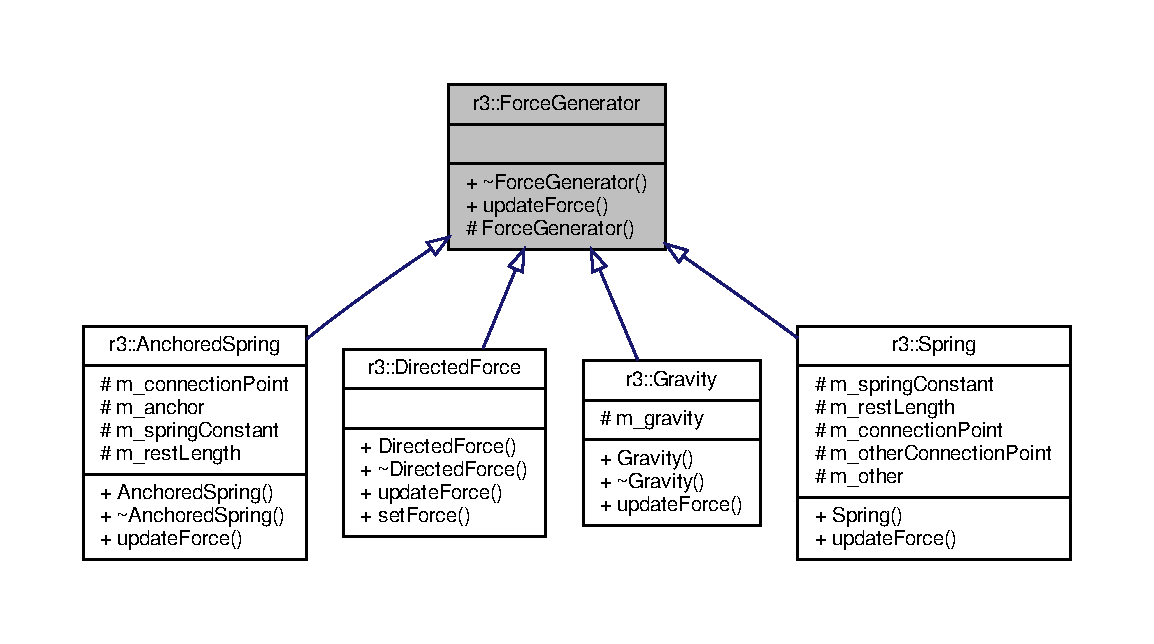
\includegraphics[width=350pt]{classr3_1_1_force_generator__inherit__graph}
\end{center}
\end{figure}


Collaboration diagram for r3\+:\+:Force\+Generator\+:\nopagebreak
\begin{figure}[H]
\begin{center}
\leavevmode
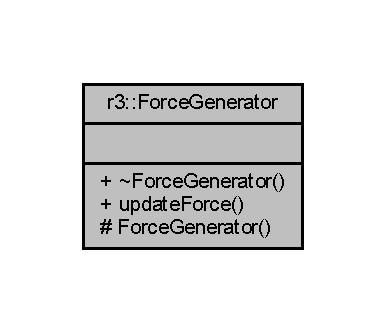
\includegraphics[width=185pt]{classr3_1_1_force_generator__coll__graph}
\end{center}
\end{figure}
\subsection*{Public Member Functions}
\begin{DoxyCompactItemize}
\item 
virtual \mbox{\hyperlink{classr3_1_1_force_generator_a64f1659bd0cf863ea28cccc689b2be3e}{$\sim$\+Force\+Generator}} ()
\item 
virtual void \mbox{\hyperlink{classr3_1_1_force_generator_a59deb54721cdcc6e33fabfb1f9a3fb27}{update\+Force}} (\mbox{\hyperlink{classr3_1_1_rigid_body}{Rigid\+Body}} $\ast$body)=0
\begin{DoxyCompactList}\small\item\em Apply force to a rigid body over a specific time. \end{DoxyCompactList}\end{DoxyCompactItemize}
\subsection*{Protected Member Functions}
\begin{DoxyCompactItemize}
\item 
\mbox{\hyperlink{classr3_1_1_force_generator_a7b21e48ccca59631975e0621057a1035}{Force\+Generator}} ()
\end{DoxyCompactItemize}


\subsection{Detailed Description}
Interface for rigid body force generators. 

\subsection{Constructor \& Destructor Documentation}
\mbox{\Hypertarget{classr3_1_1_force_generator_a64f1659bd0cf863ea28cccc689b2be3e}\label{classr3_1_1_force_generator_a64f1659bd0cf863ea28cccc689b2be3e}} 
\index{r3\+::\+Force\+Generator@{r3\+::\+Force\+Generator}!````~Force\+Generator@{$\sim$\+Force\+Generator}}
\index{````~Force\+Generator@{$\sim$\+Force\+Generator}!r3\+::\+Force\+Generator@{r3\+::\+Force\+Generator}}
\subsubsection{\texorpdfstring{$\sim$\+Force\+Generator()}{~ForceGenerator()}}
{\footnotesize\ttfamily r3\+::\+Force\+Generator\+::$\sim$\+Force\+Generator (\begin{DoxyParamCaption}{ }\end{DoxyParamCaption})\hspace{0.3cm}{\ttfamily [virtual]}, {\ttfamily [default]}}

\mbox{\Hypertarget{classr3_1_1_force_generator_a7b21e48ccca59631975e0621057a1035}\label{classr3_1_1_force_generator_a7b21e48ccca59631975e0621057a1035}} 
\index{r3\+::\+Force\+Generator@{r3\+::\+Force\+Generator}!Force\+Generator@{Force\+Generator}}
\index{Force\+Generator@{Force\+Generator}!r3\+::\+Force\+Generator@{r3\+::\+Force\+Generator}}
\subsubsection{\texorpdfstring{Force\+Generator()}{ForceGenerator()}}
{\footnotesize\ttfamily r3\+::\+Force\+Generator\+::\+Force\+Generator (\begin{DoxyParamCaption}{ }\end{DoxyParamCaption})\hspace{0.3cm}{\ttfamily [explicit]}, {\ttfamily [protected]}, {\ttfamily [default]}}



\subsection{Member Function Documentation}
\mbox{\Hypertarget{classr3_1_1_force_generator_a59deb54721cdcc6e33fabfb1f9a3fb27}\label{classr3_1_1_force_generator_a59deb54721cdcc6e33fabfb1f9a3fb27}} 
\index{r3\+::\+Force\+Generator@{r3\+::\+Force\+Generator}!update\+Force@{update\+Force}}
\index{update\+Force@{update\+Force}!r3\+::\+Force\+Generator@{r3\+::\+Force\+Generator}}
\subsubsection{\texorpdfstring{update\+Force()}{updateForce()}}
{\footnotesize\ttfamily virtual void r3\+::\+Force\+Generator\+::update\+Force (\begin{DoxyParamCaption}\item[{\mbox{\hyperlink{classr3_1_1_rigid_body}{Rigid\+Body}} $\ast$}]{body }\end{DoxyParamCaption})\hspace{0.3cm}{\ttfamily [pure virtual]}}



Apply force to a rigid body over a specific time. 


\begin{DoxyParams}{Parameters}
{\em body} & The rigid body on which to apply force. \\
\hline
{\em duration} & The duration over which the force acts. \\
\hline
\end{DoxyParams}


Implemented in \mbox{\hyperlink{classr3_1_1_spring_ab2b8d52c2a2d838b939290b29320bf66}{r3\+::\+Spring}}, \mbox{\hyperlink{classr3_1_1_anchored_spring_a56aaf13c1f89f2b45b6cb95bf16a2300}{r3\+::\+Anchored\+Spring}}, \mbox{\hyperlink{classr3_1_1_directed_force_a13dc064fe26dabe6c2803f027079e26b}{r3\+::\+Directed\+Force}}, and \mbox{\hyperlink{classr3_1_1_gravity_ae1d29cae93289b8063d8833a7107ae64}{r3\+::\+Gravity}}.



The documentation for this class was generated from the following files\+:\begin{DoxyCompactItemize}
\item 
D\+:/\+Programming/\+Repositories/\+Game\+Physics/\+Simulation\+Visualization/\+Rumble3\+D/\+Rumble3\+D/include/\+R3\+D/\+Rigid\+Body\+Engine/\mbox{\hyperlink{_force_generator_8h}{Force\+Generator.\+h}}\item 
D\+:/\+Programming/\+Repositories/\+Game\+Physics/\+Simulation\+Visualization/\+Rumble3\+D/\+Rumble3\+D/src/\+Rigid\+Body\+Engine/\mbox{\hyperlink{_force_generator_8cpp}{Force\+Generator.\+cpp}}\end{DoxyCompactItemize}

\hypertarget{structr3_1_1_force_registry_1_1_force_registration_entry}{}\section{r3\+:\+:Force\+Registry\+:\+:Force\+Registration\+Entry Struct Reference}
\label{structr3_1_1_force_registry_1_1_force_registration_entry}\index{r3\+::\+Force\+Registry\+::\+Force\+Registration\+Entry@{r3\+::\+Force\+Registry\+::\+Force\+Registration\+Entry}}


{\ttfamily \#include $<$Force\+Registry.\+h$>$}



Collaboration diagram for r3\+:\+:Force\+Registry\+:\+:Force\+Registration\+Entry\+:\nopagebreak
\begin{figure}[H]
\begin{center}
\leavevmode
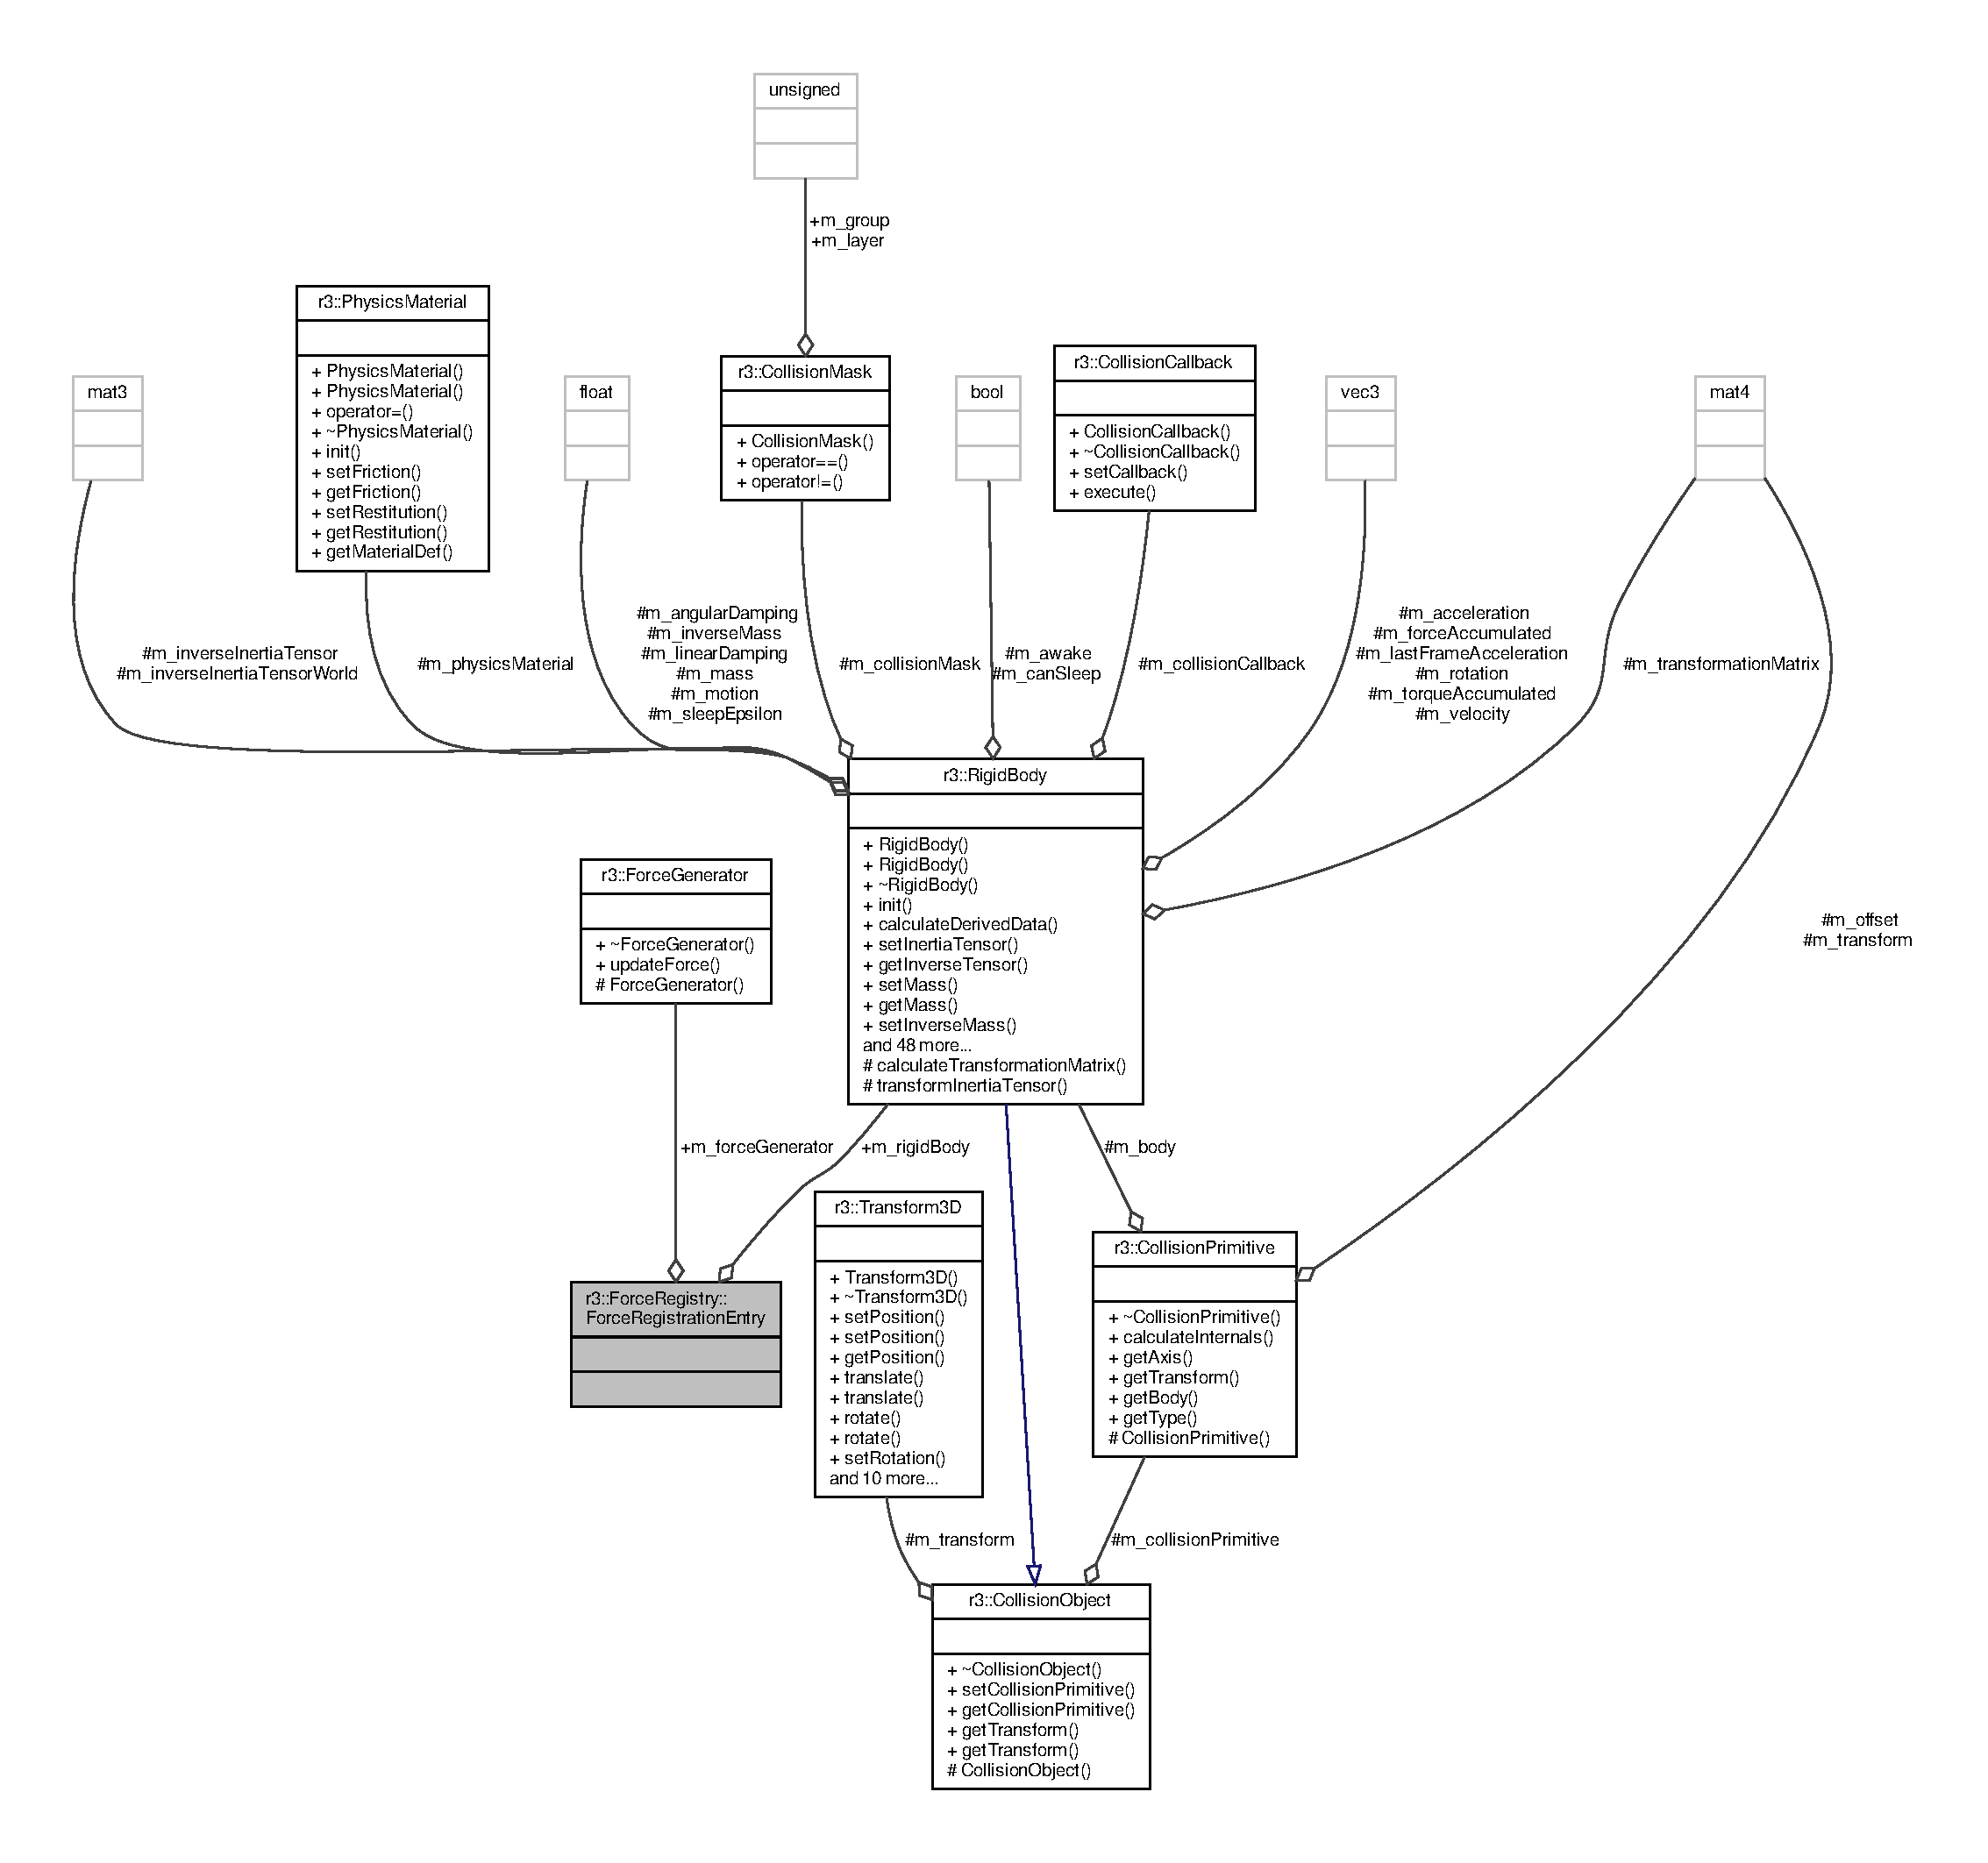
\includegraphics[width=350pt]{structr3_1_1_force_registry_1_1_force_registration_entry__coll__graph}
\end{center}
\end{figure}
\subsection*{Public Attributes}
\begin{DoxyCompactItemize}
\item 
\mbox{\hyperlink{classr3_1_1_rigid_body}{Rigid\+Body}} $\ast$ \mbox{\hyperlink{structr3_1_1_force_registry_1_1_force_registration_entry_a103ff58c0c8f46f2ed1927976bc5dc87}{m\+\_\+rigid\+Body}}
\item 
\mbox{\hyperlink{classr3_1_1_force_generator}{Force\+Generator}} $\ast$ \mbox{\hyperlink{structr3_1_1_force_registry_1_1_force_registration_entry_aa2af182d8c92d8da8d6045ea4f4a5e16}{m\+\_\+force\+Generator}}
\end{DoxyCompactItemize}


\subsection{Member Data Documentation}
\mbox{\Hypertarget{structr3_1_1_force_registry_1_1_force_registration_entry_aa2af182d8c92d8da8d6045ea4f4a5e16}\label{structr3_1_1_force_registry_1_1_force_registration_entry_aa2af182d8c92d8da8d6045ea4f4a5e16}} 
\index{r3\+::\+Force\+Registry\+::\+Force\+Registration\+Entry@{r3\+::\+Force\+Registry\+::\+Force\+Registration\+Entry}!m\+\_\+force\+Generator@{m\+\_\+force\+Generator}}
\index{m\+\_\+force\+Generator@{m\+\_\+force\+Generator}!r3\+::\+Force\+Registry\+::\+Force\+Registration\+Entry@{r3\+::\+Force\+Registry\+::\+Force\+Registration\+Entry}}
\subsubsection{\texorpdfstring{m\+\_\+force\+Generator}{m\_forceGenerator}}
{\footnotesize\ttfamily \mbox{\hyperlink{classr3_1_1_force_generator}{Force\+Generator}}$\ast$ r3\+::\+Force\+Registry\+::\+Force\+Registration\+Entry\+::m\+\_\+force\+Generator}

\mbox{\Hypertarget{structr3_1_1_force_registry_1_1_force_registration_entry_a103ff58c0c8f46f2ed1927976bc5dc87}\label{structr3_1_1_force_registry_1_1_force_registration_entry_a103ff58c0c8f46f2ed1927976bc5dc87}} 
\index{r3\+::\+Force\+Registry\+::\+Force\+Registration\+Entry@{r3\+::\+Force\+Registry\+::\+Force\+Registration\+Entry}!m\+\_\+rigid\+Body@{m\+\_\+rigid\+Body}}
\index{m\+\_\+rigid\+Body@{m\+\_\+rigid\+Body}!r3\+::\+Force\+Registry\+::\+Force\+Registration\+Entry@{r3\+::\+Force\+Registry\+::\+Force\+Registration\+Entry}}
\subsubsection{\texorpdfstring{m\+\_\+rigid\+Body}{m\_rigidBody}}
{\footnotesize\ttfamily \mbox{\hyperlink{classr3_1_1_rigid_body}{Rigid\+Body}}$\ast$ r3\+::\+Force\+Registry\+::\+Force\+Registration\+Entry\+::m\+\_\+rigid\+Body}



The documentation for this struct was generated from the following file\+:\begin{DoxyCompactItemize}
\item 
D\+:/\+Programming/\+Repositories/\+Game\+Physics/\+Simulation\+Visualization/\+Rumble3\+D/\+Rumble3\+D/include/\+R3\+D/\+Rigid\+Body\+Engine/\mbox{\hyperlink{_force_registry_8h}{Force\+Registry.\+h}}\end{DoxyCompactItemize}

\hypertarget{classr3_1_1_force_registry}{}\doxysection{r3\+::Force\+Registry Class Reference}
\label{classr3_1_1_force_registry}\index{r3::ForceRegistry@{r3::ForceRegistry}}


Pairs force generators with rigid bodies. It uses the force generators to update forces of linked rigid bodies.  




{\ttfamily \#include $<$Force\+Registry.\+h$>$}



Collaboration diagram for r3\+::Force\+Registry\+:\nopagebreak
\begin{figure}[H]
\begin{center}
\leavevmode
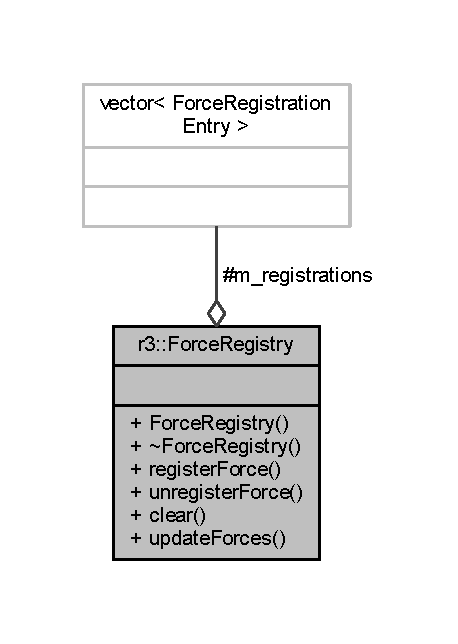
\includegraphics[width=219pt]{classr3_1_1_force_registry__coll__graph}
\end{center}
\end{figure}
\doxysubsection*{Classes}
\begin{DoxyCompactItemize}
\item 
struct \mbox{\hyperlink{structr3_1_1_force_registry_1_1_force_registration_entry}{Force\+Registration\+Entry}}
\end{DoxyCompactItemize}
\doxysubsection*{Public Types}
\begin{DoxyCompactItemize}
\item 
using \mbox{\hyperlink{classr3_1_1_force_registry_a91449a71b1a33d773ef787ae56ae9b2d}{Registry}} = std\+::vector$<$ \mbox{\hyperlink{structr3_1_1_force_registry_1_1_force_registration_entry}{Force\+Registration\+Entry}} $>$
\end{DoxyCompactItemize}
\doxysubsection*{Public Member Functions}
\begin{DoxyCompactItemize}
\item 
\mbox{\hyperlink{classr3_1_1_force_registry_a6830132c53a756ebf3e6621195f51b17}{Force\+Registry}} ()
\item 
\mbox{\hyperlink{classr3_1_1_force_registry_a322cdf54468a6f59610562a7bfc2e60d}{$\sim$\+Force\+Registry}} ()
\item 
void \mbox{\hyperlink{classr3_1_1_force_registry_a18e3bee47d4510cc91426103042b382c}{register\+Force}} (\mbox{\hyperlink{classr3_1_1_rigid_body}{Rigid\+Body}} $\ast$rigid\+Body, \mbox{\hyperlink{classr3_1_1_force_generator}{Force\+Generator}} $\ast$generator)
\begin{DoxyCompactList}\small\item\em Register a pair of rigid body and force generator. \end{DoxyCompactList}\item 
void \mbox{\hyperlink{classr3_1_1_force_registry_a8fcc46a35435ffb74c471a0a5ff36a7f}{unregister\+Force}} (\mbox{\hyperlink{classr3_1_1_rigid_body}{Rigid\+Body}} $\ast$rigid\+Body, \mbox{\hyperlink{classr3_1_1_force_generator}{Force\+Generator}} $\ast$generator)
\begin{DoxyCompactList}\small\item\em Remove a force registration entry from the registry. \end{DoxyCompactList}\item 
void \mbox{\hyperlink{classr3_1_1_force_registry_ab1c31bc403d998af16df97ff5d42c95f}{clear}} ()
\begin{DoxyCompactList}\small\item\em Remove all entries from the registry. \end{DoxyCompactList}\item 
void \mbox{\hyperlink{classr3_1_1_force_registry_a34d6ad7472e2f47dfd3416a703eca78e}{update\+Forces}} (\mbox{\hyperlink{namespacer3_ab2016b3e3f743fb735afce242f0dc1eb}{real}} duration)
\begin{DoxyCompactList}\small\item\em Use registered force generators to apply forces to rigid bodies, which they are paired up with. \end{DoxyCompactList}\end{DoxyCompactItemize}
\doxysubsection*{Protected Attributes}
\begin{DoxyCompactItemize}
\item 
\mbox{\hyperlink{classr3_1_1_force_registry_a91449a71b1a33d773ef787ae56ae9b2d}{Registry}} \mbox{\hyperlink{classr3_1_1_force_registry_a36847da26301dc4b18e6b6b25fb2fa51}{m\+\_\+registrations}}
\end{DoxyCompactItemize}


\doxysubsection{Detailed Description}
Pairs force generators with rigid bodies. It uses the force generators to update forces of linked rigid bodies. 

\doxysubsection{Member Typedef Documentation}
\mbox{\Hypertarget{classr3_1_1_force_registry_a91449a71b1a33d773ef787ae56ae9b2d}\label{classr3_1_1_force_registry_a91449a71b1a33d773ef787ae56ae9b2d}} 
\index{r3::ForceRegistry@{r3::ForceRegistry}!Registry@{Registry}}
\index{Registry@{Registry}!r3::ForceRegistry@{r3::ForceRegistry}}
\doxysubsubsection{\texorpdfstring{Registry}{Registry}}
{\footnotesize\ttfamily using \mbox{\hyperlink{classr3_1_1_force_registry_a91449a71b1a33d773ef787ae56ae9b2d}{r3\+::\+Force\+Registry\+::\+Registry}} =  std\+::vector$<$\mbox{\hyperlink{structr3_1_1_force_registry_1_1_force_registration_entry}{Force\+Registration\+Entry}}$>$}



\doxysubsection{Constructor \& Destructor Documentation}
\mbox{\Hypertarget{classr3_1_1_force_registry_a6830132c53a756ebf3e6621195f51b17}\label{classr3_1_1_force_registry_a6830132c53a756ebf3e6621195f51b17}} 
\index{r3::ForceRegistry@{r3::ForceRegistry}!ForceRegistry@{ForceRegistry}}
\index{ForceRegistry@{ForceRegistry}!r3::ForceRegistry@{r3::ForceRegistry}}
\doxysubsubsection{\texorpdfstring{ForceRegistry()}{ForceRegistry()}}
{\footnotesize\ttfamily r3\+::\+Force\+Registry\+::\+Force\+Registry (\begin{DoxyParamCaption}{ }\end{DoxyParamCaption})\hspace{0.3cm}{\ttfamily [explicit]}, {\ttfamily [default]}}

\mbox{\Hypertarget{classr3_1_1_force_registry_a322cdf54468a6f59610562a7bfc2e60d}\label{classr3_1_1_force_registry_a322cdf54468a6f59610562a7bfc2e60d}} 
\index{r3::ForceRegistry@{r3::ForceRegistry}!````~ForceRegistry@{$\sim$ForceRegistry}}
\index{````~ForceRegistry@{$\sim$ForceRegistry}!r3::ForceRegistry@{r3::ForceRegistry}}
\doxysubsubsection{\texorpdfstring{$\sim$ForceRegistry()}{~ForceRegistry()}}
{\footnotesize\ttfamily r3\+::\+Force\+Registry\+::$\sim$\+Force\+Registry (\begin{DoxyParamCaption}{ }\end{DoxyParamCaption})\hspace{0.3cm}{\ttfamily [default]}}



\doxysubsection{Member Function Documentation}
\mbox{\Hypertarget{classr3_1_1_force_registry_ab1c31bc403d998af16df97ff5d42c95f}\label{classr3_1_1_force_registry_ab1c31bc403d998af16df97ff5d42c95f}} 
\index{r3::ForceRegistry@{r3::ForceRegistry}!clear@{clear}}
\index{clear@{clear}!r3::ForceRegistry@{r3::ForceRegistry}}
\doxysubsubsection{\texorpdfstring{clear()}{clear()}}
{\footnotesize\ttfamily void r3\+::\+Force\+Registry\+::clear (\begin{DoxyParamCaption}{ }\end{DoxyParamCaption})}



Remove all entries from the registry. 

\mbox{\Hypertarget{classr3_1_1_force_registry_a18e3bee47d4510cc91426103042b382c}\label{classr3_1_1_force_registry_a18e3bee47d4510cc91426103042b382c}} 
\index{r3::ForceRegistry@{r3::ForceRegistry}!registerForce@{registerForce}}
\index{registerForce@{registerForce}!r3::ForceRegistry@{r3::ForceRegistry}}
\doxysubsubsection{\texorpdfstring{registerForce()}{registerForce()}}
{\footnotesize\ttfamily void r3\+::\+Force\+Registry\+::register\+Force (\begin{DoxyParamCaption}\item[{\mbox{\hyperlink{classr3_1_1_rigid_body}{Rigid\+Body}} $\ast$}]{rigid\+Body,  }\item[{\mbox{\hyperlink{classr3_1_1_force_generator}{Force\+Generator}} $\ast$}]{generator }\end{DoxyParamCaption})}



Register a pair of rigid body and force generator. 


\begin{DoxyParams}{Parameters}
{\em rigid\+Body} & The rigid body part of the pair. \\
\hline
{\em generator} & The force generator part of the pair. \\
\hline
\end{DoxyParams}
\mbox{\Hypertarget{classr3_1_1_force_registry_a8fcc46a35435ffb74c471a0a5ff36a7f}\label{classr3_1_1_force_registry_a8fcc46a35435ffb74c471a0a5ff36a7f}} 
\index{r3::ForceRegistry@{r3::ForceRegistry}!unregisterForce@{unregisterForce}}
\index{unregisterForce@{unregisterForce}!r3::ForceRegistry@{r3::ForceRegistry}}
\doxysubsubsection{\texorpdfstring{unregisterForce()}{unregisterForce()}}
{\footnotesize\ttfamily void r3\+::\+Force\+Registry\+::unregister\+Force (\begin{DoxyParamCaption}\item[{\mbox{\hyperlink{classr3_1_1_rigid_body}{Rigid\+Body}} $\ast$}]{rigid\+Body,  }\item[{\mbox{\hyperlink{classr3_1_1_force_generator}{Force\+Generator}} $\ast$}]{generator }\end{DoxyParamCaption})}



Remove a force registration entry from the registry. 


\begin{DoxyParams}{Parameters}
{\em rigid\+Body} & The rigid body part of the entry. \\
\hline
{\em generator} & The generator part of the entry. \\
\hline
\end{DoxyParams}
\mbox{\Hypertarget{classr3_1_1_force_registry_a34d6ad7472e2f47dfd3416a703eca78e}\label{classr3_1_1_force_registry_a34d6ad7472e2f47dfd3416a703eca78e}} 
\index{r3::ForceRegistry@{r3::ForceRegistry}!updateForces@{updateForces}}
\index{updateForces@{updateForces}!r3::ForceRegistry@{r3::ForceRegistry}}
\doxysubsubsection{\texorpdfstring{updateForces()}{updateForces()}}
{\footnotesize\ttfamily void r3\+::\+Force\+Registry\+::update\+Forces (\begin{DoxyParamCaption}\item[{\mbox{\hyperlink{namespacer3_ab2016b3e3f743fb735afce242f0dc1eb}{real}}}]{duration }\end{DoxyParamCaption})}



Use registered force generators to apply forces to rigid bodies, which they are paired up with. 


\begin{DoxyParams}{Parameters}
{\em duration} & Time step of the simulation update. \\
\hline
\end{DoxyParams}


\doxysubsection{Member Data Documentation}
\mbox{\Hypertarget{classr3_1_1_force_registry_a36847da26301dc4b18e6b6b25fb2fa51}\label{classr3_1_1_force_registry_a36847da26301dc4b18e6b6b25fb2fa51}} 
\index{r3::ForceRegistry@{r3::ForceRegistry}!m\_registrations@{m\_registrations}}
\index{m\_registrations@{m\_registrations}!r3::ForceRegistry@{r3::ForceRegistry}}
\doxysubsubsection{\texorpdfstring{m\_registrations}{m\_registrations}}
{\footnotesize\ttfamily \mbox{\hyperlink{classr3_1_1_force_registry_a91449a71b1a33d773ef787ae56ae9b2d}{Registry}} r3\+::\+Force\+Registry\+::m\+\_\+registrations\hspace{0.3cm}{\ttfamily [protected]}}



The documentation for this class was generated from the following files\+:\begin{DoxyCompactItemize}
\item 
/home/nelaty/\+Development/\+Repositories/\+Rumble3\+D/include/\+R3\+D/\+Rigid\+Body\+Engine/\mbox{\hyperlink{_force_registry_8h}{Force\+Registry.\+h}}\item 
/home/nelaty/\+Development/\+Repositories/\+Rumble3\+D/src/\+Rigid\+Body\+Engine/\mbox{\hyperlink{_force_registry_8cpp}{Force\+Registry.\+cpp}}\end{DoxyCompactItemize}

\hypertarget{classr3_1_1_friction_resolver}{}\section{r3\+:\+:Friction\+Resolver Class Reference}
\label{classr3_1_1_friction_resolver}\index{r3\+::\+Friction\+Resolver@{r3\+::\+Friction\+Resolver}}


Specialized collision resolution filter, which adds friction at given contacts.  




{\ttfamily \#include $<$Friction\+Resolver.\+h$>$}



Inheritance diagram for r3\+:\+:Friction\+Resolver\+:\nopagebreak
\begin{figure}[H]
\begin{center}
\leavevmode
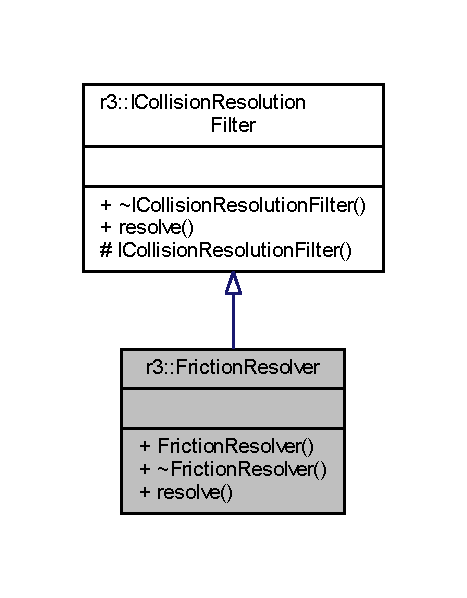
\includegraphics[width=224pt]{classr3_1_1_friction_resolver__inherit__graph}
\end{center}
\end{figure}


Collaboration diagram for r3\+:\+:Friction\+Resolver\+:\nopagebreak
\begin{figure}[H]
\begin{center}
\leavevmode
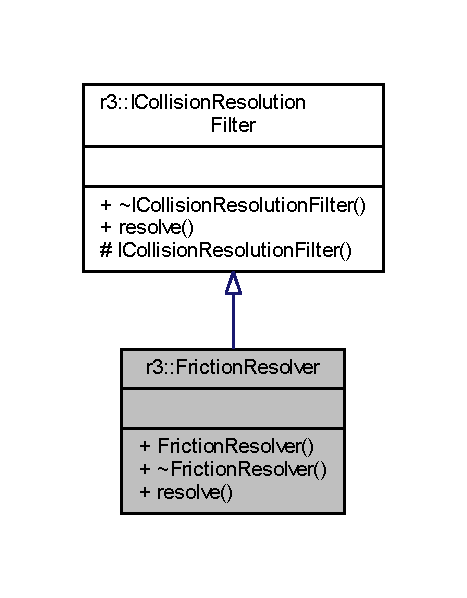
\includegraphics[width=224pt]{classr3_1_1_friction_resolver__coll__graph}
\end{center}
\end{figure}
\subsection*{Public Member Functions}
\begin{DoxyCompactItemize}
\item 
\mbox{\hyperlink{classr3_1_1_friction_resolver_a55a3a08603cf362da1896ec2ccc026ba}{Friction\+Resolver}} ()
\item 
\mbox{\hyperlink{classr3_1_1_friction_resolver_a49a41d6820e9c9c17447c79303296dea}{$\sim$\+Friction\+Resolver}} ()
\item 
void \mbox{\hyperlink{classr3_1_1_friction_resolver_af26a84959e95749088f713176ec3c096}{resolve}} (\mbox{\hyperlink{classr3_1_1_collision_data}{Collision\+Data}} \&collision\+Data, \mbox{\hyperlink{namespacer3_ab2016b3e3f743fb735afce242f0dc1eb}{real}} time\+Delta) override
\begin{DoxyCompactList}\small\item\em Resolve given contacts. \end{DoxyCompactList}\end{DoxyCompactItemize}
\subsection*{Additional Inherited Members}


\subsection{Detailed Description}
Specialized collision resolution filter, which adds friction at given contacts. 

\subsection{Constructor \& Destructor Documentation}
\mbox{\Hypertarget{classr3_1_1_friction_resolver_a55a3a08603cf362da1896ec2ccc026ba}\label{classr3_1_1_friction_resolver_a55a3a08603cf362da1896ec2ccc026ba}} 
\index{r3\+::\+Friction\+Resolver@{r3\+::\+Friction\+Resolver}!Friction\+Resolver@{Friction\+Resolver}}
\index{Friction\+Resolver@{Friction\+Resolver}!r3\+::\+Friction\+Resolver@{r3\+::\+Friction\+Resolver}}
\subsubsection{\texorpdfstring{Friction\+Resolver()}{FrictionResolver()}}
{\footnotesize\ttfamily r3\+::\+Friction\+Resolver\+::\+Friction\+Resolver (\begin{DoxyParamCaption}{ }\end{DoxyParamCaption})\hspace{0.3cm}{\ttfamily [explicit]}, {\ttfamily [default]}}

\mbox{\Hypertarget{classr3_1_1_friction_resolver_a49a41d6820e9c9c17447c79303296dea}\label{classr3_1_1_friction_resolver_a49a41d6820e9c9c17447c79303296dea}} 
\index{r3\+::\+Friction\+Resolver@{r3\+::\+Friction\+Resolver}!````~Friction\+Resolver@{$\sim$\+Friction\+Resolver}}
\index{````~Friction\+Resolver@{$\sim$\+Friction\+Resolver}!r3\+::\+Friction\+Resolver@{r3\+::\+Friction\+Resolver}}
\subsubsection{\texorpdfstring{$\sim$\+Friction\+Resolver()}{~FrictionResolver()}}
{\footnotesize\ttfamily r3\+::\+Friction\+Resolver\+::$\sim$\+Friction\+Resolver (\begin{DoxyParamCaption}{ }\end{DoxyParamCaption})\hspace{0.3cm}{\ttfamily [default]}}



\subsection{Member Function Documentation}
\mbox{\Hypertarget{classr3_1_1_friction_resolver_af26a84959e95749088f713176ec3c096}\label{classr3_1_1_friction_resolver_af26a84959e95749088f713176ec3c096}} 
\index{r3\+::\+Friction\+Resolver@{r3\+::\+Friction\+Resolver}!resolve@{resolve}}
\index{resolve@{resolve}!r3\+::\+Friction\+Resolver@{r3\+::\+Friction\+Resolver}}
\subsubsection{\texorpdfstring{resolve()}{resolve()}}
{\footnotesize\ttfamily void r3\+::\+Friction\+Resolver\+::resolve (\begin{DoxyParamCaption}\item[{\mbox{\hyperlink{classr3_1_1_collision_data}{Collision\+Data}} \&}]{collision\+Data,  }\item[{\mbox{\hyperlink{namespacer3_ab2016b3e3f743fb735afce242f0dc1eb}{real}}}]{time\+Delta }\end{DoxyParamCaption})\hspace{0.3cm}{\ttfamily [override]}, {\ttfamily [virtual]}}



Resolve given contacts. 


\begin{DoxyParams}{Parameters}
{\em collision\+Data} & The contacts to resolve. \\
\hline
{\em time\+Delta} & The time step of the current physics update. \\
\hline
\end{DoxyParams}


Implements \mbox{\hyperlink{classr3_1_1_i_collision_resolution_filter_a87ef2579e2acaaadef4cd8f9a20005ce}{r3\+::\+I\+Collision\+Resolution\+Filter}}.



The documentation for this class was generated from the following files\+:\begin{DoxyCompactItemize}
\item 
D\+:/\+Programming/\+Repositories/\+Game\+Physics/\+Simulation\+Visualization/\+Rumble3\+D/\+Rumble3\+D/include/\+R3\+D/\+Rigid\+Body\+Engine/\+Collision\+Resolution/\mbox{\hyperlink{_friction_resolver_8h}{Friction\+Resolver.\+h}}\item 
D\+:/\+Programming/\+Repositories/\+Game\+Physics/\+Simulation\+Visualization/\+Rumble3\+D/\+Rumble3\+D/src/\+Rigid\+Body\+Engine/\+Collision\+Resolution/\mbox{\hyperlink{_friction_resolver_8cpp}{Friction\+Resolver.\+cpp}}\end{DoxyCompactItemize}

\hypertarget{classr3_1_1_gravity}{}\section{r3\+:\+:Gravity Class Reference}
\label{classr3_1_1_gravity}\index{r3\+::\+Gravity@{r3\+::\+Gravity}}


\mbox{\hyperlink{classr3_1_1_gravity}{Gravity}} is a force generator, which will apply constant force on bodies.  




{\ttfamily \#include $<$Gravity.\+h$>$}



Inheritance diagram for r3\+:\+:Gravity\+:\nopagebreak
\begin{figure}[H]
\begin{center}
\leavevmode
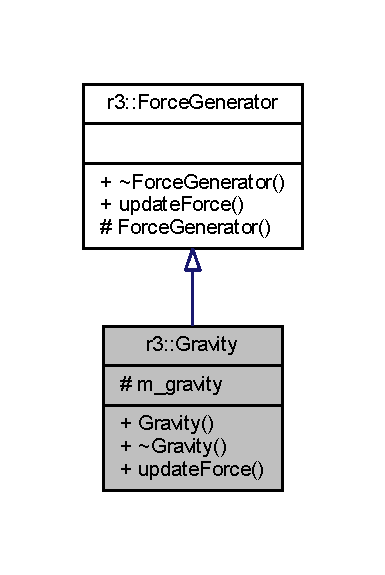
\includegraphics[width=185pt]{classr3_1_1_gravity__inherit__graph}
\end{center}
\end{figure}


Collaboration diagram for r3\+:\+:Gravity\+:\nopagebreak
\begin{figure}[H]
\begin{center}
\leavevmode
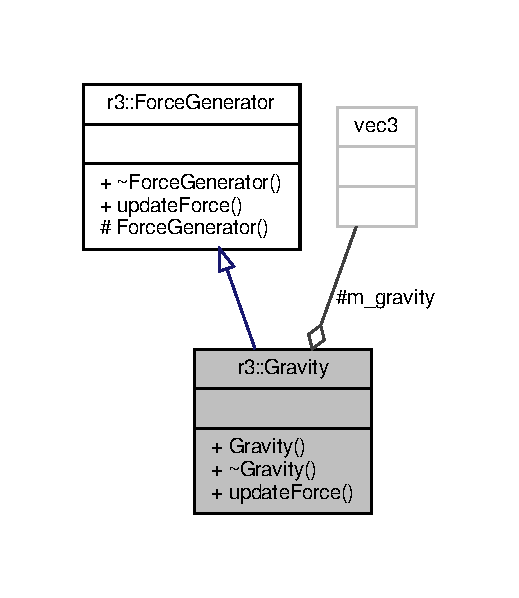
\includegraphics[width=251pt]{classr3_1_1_gravity__coll__graph}
\end{center}
\end{figure}
\subsection*{Public Member Functions}
\begin{DoxyCompactItemize}
\item 
\mbox{\hyperlink{classr3_1_1_gravity_a1c5f6d085a7b1484c23f5a6df4b58b05}{Gravity}} (const glm\+::vec3 \&gravity)
\begin{DoxyCompactList}\small\item\em \mbox{\hyperlink{classr3_1_1_gravity}{Gravity}} constructor. \end{DoxyCompactList}\item 
\mbox{\hyperlink{classr3_1_1_gravity_abdf3edf32d08b6c5b9c2fc161635f993}{$\sim$\+Gravity}} ()
\item 
void \mbox{\hyperlink{classr3_1_1_gravity_ae1d29cae93289b8063d8833a7107ae64}{update\+Force}} (\mbox{\hyperlink{classr3_1_1_rigid_body}{Rigid\+Body}} $\ast$body) override
\begin{DoxyCompactList}\small\item\em Apply force to a rigid body over a specific time. \end{DoxyCompactList}\end{DoxyCompactItemize}
\subsection*{Protected Attributes}
\begin{DoxyCompactItemize}
\item 
glm\+::vec3 \mbox{\hyperlink{classr3_1_1_gravity_a2feb1d84fc4118e6e30b707a7224f6ef}{m\+\_\+gravity}}
\end{DoxyCompactItemize}
\subsection*{Additional Inherited Members}


\subsection{Detailed Description}
\mbox{\hyperlink{classr3_1_1_gravity}{Gravity}} is a force generator, which will apply constant force on bodies. 

\subsection{Constructor \& Destructor Documentation}
\mbox{\Hypertarget{classr3_1_1_gravity_a1c5f6d085a7b1484c23f5a6df4b58b05}\label{classr3_1_1_gravity_a1c5f6d085a7b1484c23f5a6df4b58b05}} 
\index{r3\+::\+Gravity@{r3\+::\+Gravity}!Gravity@{Gravity}}
\index{Gravity@{Gravity}!r3\+::\+Gravity@{r3\+::\+Gravity}}
\subsubsection{\texorpdfstring{Gravity()}{Gravity()}}
{\footnotesize\ttfamily r3\+::\+Gravity\+::\+Gravity (\begin{DoxyParamCaption}\item[{const glm\+::vec3 \&}]{gravity }\end{DoxyParamCaption})\hspace{0.3cm}{\ttfamily [explicit]}}



\mbox{\hyperlink{classr3_1_1_gravity}{Gravity}} constructor. 


\begin{DoxyParams}{Parameters}
{\em gravity} & A constant force. \\
\hline
\end{DoxyParams}
\mbox{\Hypertarget{classr3_1_1_gravity_abdf3edf32d08b6c5b9c2fc161635f993}\label{classr3_1_1_gravity_abdf3edf32d08b6c5b9c2fc161635f993}} 
\index{r3\+::\+Gravity@{r3\+::\+Gravity}!````~Gravity@{$\sim$\+Gravity}}
\index{````~Gravity@{$\sim$\+Gravity}!r3\+::\+Gravity@{r3\+::\+Gravity}}
\subsubsection{\texorpdfstring{$\sim$\+Gravity()}{~Gravity()}}
{\footnotesize\ttfamily r3\+::\+Gravity\+::$\sim$\+Gravity (\begin{DoxyParamCaption}{ }\end{DoxyParamCaption})\hspace{0.3cm}{\ttfamily [default]}}



\subsection{Member Function Documentation}
\mbox{\Hypertarget{classr3_1_1_gravity_ae1d29cae93289b8063d8833a7107ae64}\label{classr3_1_1_gravity_ae1d29cae93289b8063d8833a7107ae64}} 
\index{r3\+::\+Gravity@{r3\+::\+Gravity}!update\+Force@{update\+Force}}
\index{update\+Force@{update\+Force}!r3\+::\+Gravity@{r3\+::\+Gravity}}
\subsubsection{\texorpdfstring{update\+Force()}{updateForce()}}
{\footnotesize\ttfamily void r3\+::\+Gravity\+::update\+Force (\begin{DoxyParamCaption}\item[{\mbox{\hyperlink{classr3_1_1_rigid_body}{Rigid\+Body}} $\ast$}]{body }\end{DoxyParamCaption})\hspace{0.3cm}{\ttfamily [override]}, {\ttfamily [virtual]}}



Apply force to a rigid body over a specific time. 


\begin{DoxyParams}{Parameters}
{\em body} & The rigid body on which to apply force. \\
\hline
\end{DoxyParams}


Implements \mbox{\hyperlink{classr3_1_1_force_generator_a59deb54721cdcc6e33fabfb1f9a3fb27}{r3\+::\+Force\+Generator}}.



\subsection{Member Data Documentation}
\mbox{\Hypertarget{classr3_1_1_gravity_a2feb1d84fc4118e6e30b707a7224f6ef}\label{classr3_1_1_gravity_a2feb1d84fc4118e6e30b707a7224f6ef}} 
\index{r3\+::\+Gravity@{r3\+::\+Gravity}!m\+\_\+gravity@{m\+\_\+gravity}}
\index{m\+\_\+gravity@{m\+\_\+gravity}!r3\+::\+Gravity@{r3\+::\+Gravity}}
\subsubsection{\texorpdfstring{m\+\_\+gravity}{m\_gravity}}
{\footnotesize\ttfamily glm\+::vec3 r3\+::\+Gravity\+::m\+\_\+gravity\hspace{0.3cm}{\ttfamily [protected]}}



The documentation for this class was generated from the following files\+:\begin{DoxyCompactItemize}
\item 
D\+:/\+Programming/\+Repositories/\+Game\+Physics/\+Simulation\+Visualization/\+Rumble3\+D/\+Rumble3\+D/include/\+R3\+D/\+Rigid\+Body\+Engine/\mbox{\hyperlink{_gravity_8h}{Gravity.\+h}}\item 
D\+:/\+Programming/\+Repositories/\+Game\+Physics/\+Simulation\+Visualization/\+Rumble3\+D/\+Rumble3\+D/src/\+Rigid\+Body\+Engine/\mbox{\hyperlink{_gravity_8cpp}{Gravity.\+cpp}}\end{DoxyCompactItemize}

\hypertarget{classr3_1_1_i_box_box_narrow_algorithm}{}\section{r3\+:\+:I\+Box\+Box\+Narrow\+Algorithm Class Reference}
\label{classr3_1_1_i_box_box_narrow_algorithm}\index{r3\+::\+I\+Box\+Box\+Narrow\+Algorithm@{r3\+::\+I\+Box\+Box\+Narrow\+Algorithm}}


Interface for box-\/box narrow algorithms.  




{\ttfamily \#include $<$I\+Box\+Box\+Narrow\+Algorithm.\+h$>$}



Inheritance diagram for r3\+:\+:I\+Box\+Box\+Narrow\+Algorithm\+:\nopagebreak
\begin{figure}[H]
\begin{center}
\leavevmode
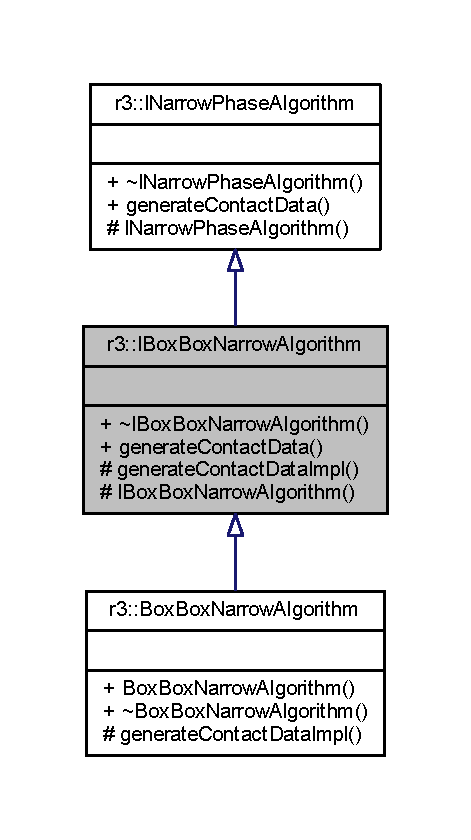
\includegraphics[width=226pt]{classr3_1_1_i_box_box_narrow_algorithm__inherit__graph}
\end{center}
\end{figure}


Collaboration diagram for r3\+:\+:I\+Box\+Box\+Narrow\+Algorithm\+:\nopagebreak
\begin{figure}[H]
\begin{center}
\leavevmode
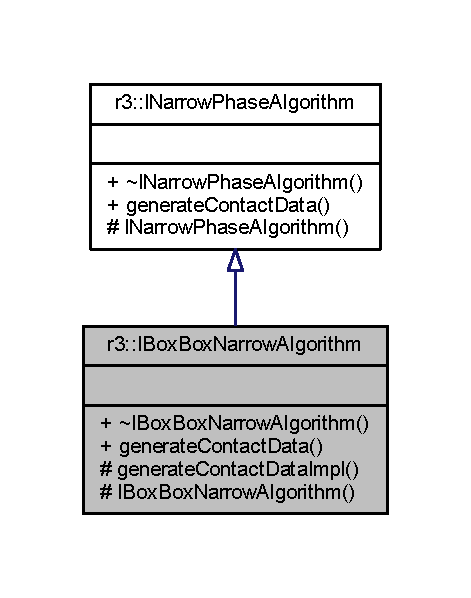
\includegraphics[width=226pt]{classr3_1_1_i_box_box_narrow_algorithm__coll__graph}
\end{center}
\end{figure}
\subsection*{Public Member Functions}
\begin{DoxyCompactItemize}
\item 
virtual \mbox{\hyperlink{classr3_1_1_i_box_box_narrow_algorithm_a384c60f79ed845100877e62d7e2a10f4}{$\sim$\+I\+Box\+Box\+Narrow\+Algorithm}} ()
\item 
bool \mbox{\hyperlink{classr3_1_1_i_box_box_narrow_algorithm_a4b06ee2be38c248c59195082db64c3e3}{generate\+Contact\+Data}} (\mbox{\hyperlink{classr3_1_1_rigid_body}{Rigid\+Body}} $\ast$first, \mbox{\hyperlink{classr3_1_1_rigid_body}{Rigid\+Body}} $\ast$second, \mbox{\hyperlink{classr3_1_1_collision_data}{Collision\+Data}} \&collision\+Data) override final
\begin{DoxyCompactList}\small\item\em Generate contacts between two rigid bodies. \end{DoxyCompactList}\end{DoxyCompactItemize}
\subsection*{Protected Member Functions}
\begin{DoxyCompactItemize}
\item 
virtual bool \mbox{\hyperlink{classr3_1_1_i_box_box_narrow_algorithm_abc15898100b5ed0537e4c6ccc6610069}{generate\+Contact\+Data\+Impl}} (\mbox{\hyperlink{classr3_1_1_rigid_body}{Rigid\+Body}} $\ast$rb\+Box1, \mbox{\hyperlink{classr3_1_1_collision_box}{Collision\+Box}} $\ast$box1, \mbox{\hyperlink{classr3_1_1_rigid_body}{Rigid\+Body}} $\ast$rb\+Box2, \mbox{\hyperlink{classr3_1_1_collision_box}{Collision\+Box}} $\ast$box2, \mbox{\hyperlink{classr3_1_1_collision_data}{Collision\+Data}} \&collision\+Data)=0
\item 
\mbox{\hyperlink{classr3_1_1_i_box_box_narrow_algorithm_a9e01be1ba6e1bbd925fca03f36f06752}{I\+Box\+Box\+Narrow\+Algorithm}} ()
\end{DoxyCompactItemize}


\subsection{Detailed Description}
Interface for box-\/box narrow algorithms. 

\subsection{Constructor \& Destructor Documentation}
\mbox{\Hypertarget{classr3_1_1_i_box_box_narrow_algorithm_a384c60f79ed845100877e62d7e2a10f4}\label{classr3_1_1_i_box_box_narrow_algorithm_a384c60f79ed845100877e62d7e2a10f4}} 
\index{r3\+::\+I\+Box\+Box\+Narrow\+Algorithm@{r3\+::\+I\+Box\+Box\+Narrow\+Algorithm}!````~I\+Box\+Box\+Narrow\+Algorithm@{$\sim$\+I\+Box\+Box\+Narrow\+Algorithm}}
\index{````~I\+Box\+Box\+Narrow\+Algorithm@{$\sim$\+I\+Box\+Box\+Narrow\+Algorithm}!r3\+::\+I\+Box\+Box\+Narrow\+Algorithm@{r3\+::\+I\+Box\+Box\+Narrow\+Algorithm}}
\subsubsection{\texorpdfstring{$\sim$\+I\+Box\+Box\+Narrow\+Algorithm()}{~IBoxBoxNarrowAlgorithm()}}
{\footnotesize\ttfamily r3\+::\+I\+Box\+Box\+Narrow\+Algorithm\+::$\sim$\+I\+Box\+Box\+Narrow\+Algorithm (\begin{DoxyParamCaption}{ }\end{DoxyParamCaption})\hspace{0.3cm}{\ttfamily [virtual]}, {\ttfamily [default]}}

\mbox{\Hypertarget{classr3_1_1_i_box_box_narrow_algorithm_a9e01be1ba6e1bbd925fca03f36f06752}\label{classr3_1_1_i_box_box_narrow_algorithm_a9e01be1ba6e1bbd925fca03f36f06752}} 
\index{r3\+::\+I\+Box\+Box\+Narrow\+Algorithm@{r3\+::\+I\+Box\+Box\+Narrow\+Algorithm}!I\+Box\+Box\+Narrow\+Algorithm@{I\+Box\+Box\+Narrow\+Algorithm}}
\index{I\+Box\+Box\+Narrow\+Algorithm@{I\+Box\+Box\+Narrow\+Algorithm}!r3\+::\+I\+Box\+Box\+Narrow\+Algorithm@{r3\+::\+I\+Box\+Box\+Narrow\+Algorithm}}
\subsubsection{\texorpdfstring{I\+Box\+Box\+Narrow\+Algorithm()}{IBoxBoxNarrowAlgorithm()}}
{\footnotesize\ttfamily r3\+::\+I\+Box\+Box\+Narrow\+Algorithm\+::\+I\+Box\+Box\+Narrow\+Algorithm (\begin{DoxyParamCaption}{ }\end{DoxyParamCaption})\hspace{0.3cm}{\ttfamily [explicit]}, {\ttfamily [protected]}, {\ttfamily [default]}}



\subsection{Member Function Documentation}
\mbox{\Hypertarget{classr3_1_1_i_box_box_narrow_algorithm_a4b06ee2be38c248c59195082db64c3e3}\label{classr3_1_1_i_box_box_narrow_algorithm_a4b06ee2be38c248c59195082db64c3e3}} 
\index{r3\+::\+I\+Box\+Box\+Narrow\+Algorithm@{r3\+::\+I\+Box\+Box\+Narrow\+Algorithm}!generate\+Contact\+Data@{generate\+Contact\+Data}}
\index{generate\+Contact\+Data@{generate\+Contact\+Data}!r3\+::\+I\+Box\+Box\+Narrow\+Algorithm@{r3\+::\+I\+Box\+Box\+Narrow\+Algorithm}}
\subsubsection{\texorpdfstring{generate\+Contact\+Data()}{generateContactData()}}
{\footnotesize\ttfamily bool r3\+::\+I\+Box\+Box\+Narrow\+Algorithm\+::generate\+Contact\+Data (\begin{DoxyParamCaption}\item[{\mbox{\hyperlink{classr3_1_1_rigid_body}{Rigid\+Body}} $\ast$}]{first,  }\item[{\mbox{\hyperlink{classr3_1_1_rigid_body}{Rigid\+Body}} $\ast$}]{second,  }\item[{\mbox{\hyperlink{classr3_1_1_collision_data}{Collision\+Data}} \&}]{collision\+Data }\end{DoxyParamCaption})\hspace{0.3cm}{\ttfamily [final]}, {\ttfamily [override]}, {\ttfamily [virtual]}}



Generate contacts between two rigid bodies. 


\begin{DoxyParams}{Parameters}
{\em first} & The first participating rigid body. \\
\hline
{\em second} & The second participating rigid body. \\
\hline
{\em collision\+Data} & All newly generated contacts will be put in here. \\
\hline
\end{DoxyParams}
\begin{DoxyReturn}{Returns}
True if new contacts have been generated, false otherwise. 
\end{DoxyReturn}


Implements \mbox{\hyperlink{classr3_1_1_i_narrow_phase_algorithm_a606fe8de5fe81ff45fedb81ca74717c3}{r3\+::\+I\+Narrow\+Phase\+Algorithm}}.

\mbox{\Hypertarget{classr3_1_1_i_box_box_narrow_algorithm_abc15898100b5ed0537e4c6ccc6610069}\label{classr3_1_1_i_box_box_narrow_algorithm_abc15898100b5ed0537e4c6ccc6610069}} 
\index{r3\+::\+I\+Box\+Box\+Narrow\+Algorithm@{r3\+::\+I\+Box\+Box\+Narrow\+Algorithm}!generate\+Contact\+Data\+Impl@{generate\+Contact\+Data\+Impl}}
\index{generate\+Contact\+Data\+Impl@{generate\+Contact\+Data\+Impl}!r3\+::\+I\+Box\+Box\+Narrow\+Algorithm@{r3\+::\+I\+Box\+Box\+Narrow\+Algorithm}}
\subsubsection{\texorpdfstring{generate\+Contact\+Data\+Impl()}{generateContactDataImpl()}}
{\footnotesize\ttfamily virtual bool r3\+::\+I\+Box\+Box\+Narrow\+Algorithm\+::generate\+Contact\+Data\+Impl (\begin{DoxyParamCaption}\item[{\mbox{\hyperlink{classr3_1_1_rigid_body}{Rigid\+Body}} $\ast$}]{rb\+Box1,  }\item[{\mbox{\hyperlink{classr3_1_1_collision_box}{Collision\+Box}} $\ast$}]{box1,  }\item[{\mbox{\hyperlink{classr3_1_1_rigid_body}{Rigid\+Body}} $\ast$}]{rb\+Box2,  }\item[{\mbox{\hyperlink{classr3_1_1_collision_box}{Collision\+Box}} $\ast$}]{box2,  }\item[{\mbox{\hyperlink{classr3_1_1_collision_data}{Collision\+Data}} \&}]{collision\+Data }\end{DoxyParamCaption})\hspace{0.3cm}{\ttfamily [protected]}, {\ttfamily [pure virtual]}}



Implemented in \mbox{\hyperlink{classr3_1_1_box_box_narrow_algorithm_a200098ad4e6e2381f58856002a2d5dec}{r3\+::\+Box\+Box\+Narrow\+Algorithm}}.



The documentation for this class was generated from the following files\+:\begin{DoxyCompactItemize}
\item 
D\+:/\+Programming/\+Repositories/\+Game\+Physics/\+Simulation\+Visualization/\+Rumble3\+D/\+Rumble3\+D/include/\+R3\+D/\+Rigid\+Body\+Engine/\+Collision\+Detection/\+Algorithm/\mbox{\hyperlink{_i_box_box_narrow_algorithm_8h}{I\+Box\+Box\+Narrow\+Algorithm.\+h}}\item 
D\+:/\+Programming/\+Repositories/\+Game\+Physics/\+Simulation\+Visualization/\+Rumble3\+D/\+Rumble3\+D/src/\+Rigid\+Body\+Engine/\+Collision\+Detection/\+Algorithm/\mbox{\hyperlink{_i_box_box_narrow_algorithm_8cpp}{I\+Box\+Box\+Narrow\+Algorithm.\+cpp}}\end{DoxyCompactItemize}

\hypertarget{classr3_1_1_i_box_sphere_narrow_algorithm}{}\section{r3\+:\+:I\+Box\+Sphere\+Narrow\+Algorithm Class Reference}
\label{classr3_1_1_i_box_sphere_narrow_algorithm}\index{r3\+::\+I\+Box\+Sphere\+Narrow\+Algorithm@{r3\+::\+I\+Box\+Sphere\+Narrow\+Algorithm}}


Interface for box-\/sphere narrow algorithms.  




{\ttfamily \#include $<$I\+Box\+Sphere\+Narrow\+Algorithm.\+h$>$}



Inheritance diagram for r3\+:\+:I\+Box\+Sphere\+Narrow\+Algorithm\+:\nopagebreak
\begin{figure}[H]
\begin{center}
\leavevmode
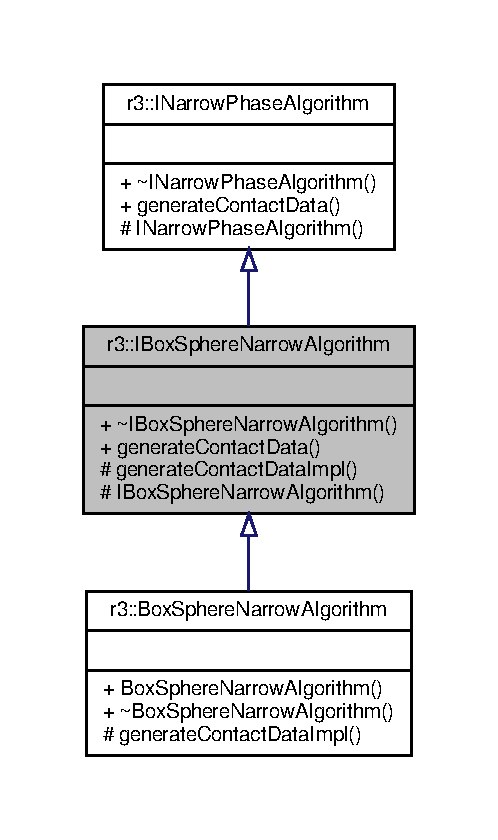
\includegraphics[width=239pt]{classr3_1_1_i_box_sphere_narrow_algorithm__inherit__graph}
\end{center}
\end{figure}


Collaboration diagram for r3\+:\+:I\+Box\+Sphere\+Narrow\+Algorithm\+:\nopagebreak
\begin{figure}[H]
\begin{center}
\leavevmode
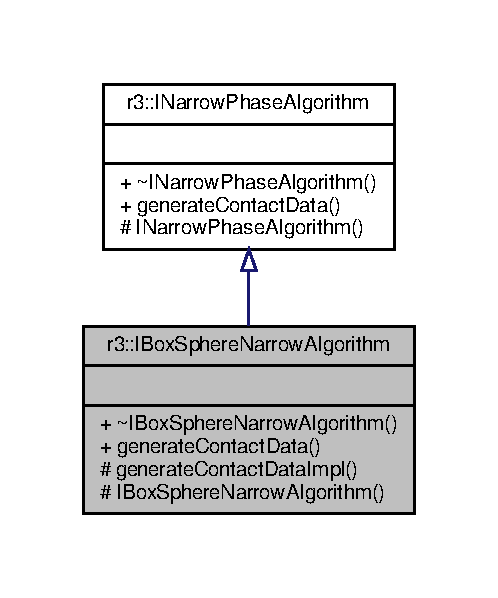
\includegraphics[width=239pt]{classr3_1_1_i_box_sphere_narrow_algorithm__coll__graph}
\end{center}
\end{figure}
\subsection*{Public Member Functions}
\begin{DoxyCompactItemize}
\item 
virtual \mbox{\hyperlink{classr3_1_1_i_box_sphere_narrow_algorithm_ac70f8e99bb2deb52c1e4686ef6fafe2d}{$\sim$\+I\+Box\+Sphere\+Narrow\+Algorithm}} ()
\item 
bool \mbox{\hyperlink{classr3_1_1_i_box_sphere_narrow_algorithm_aeecdb2486c6e6cbae057466f05323bdb}{generate\+Contact\+Data}} (\mbox{\hyperlink{classr3_1_1_rigid_body}{Rigid\+Body}} $\ast$first, \mbox{\hyperlink{classr3_1_1_rigid_body}{Rigid\+Body}} $\ast$second, \mbox{\hyperlink{classr3_1_1_collision_data}{Collision\+Data}} \&collision\+Data) override final
\begin{DoxyCompactList}\small\item\em Generate contacts between two rigid bodies. \end{DoxyCompactList}\end{DoxyCompactItemize}
\subsection*{Protected Member Functions}
\begin{DoxyCompactItemize}
\item 
virtual bool \mbox{\hyperlink{classr3_1_1_i_box_sphere_narrow_algorithm_af28bcda3eb527a6ee48a3b624e5d47e0}{generate\+Contact\+Data\+Impl}} (\mbox{\hyperlink{classr3_1_1_rigid_body}{Rigid\+Body}} $\ast$rb\+Box, \mbox{\hyperlink{classr3_1_1_collision_box}{Collision\+Box}} $\ast$box, \mbox{\hyperlink{classr3_1_1_rigid_body}{Rigid\+Body}} $\ast$rb\+Sphere, \mbox{\hyperlink{classr3_1_1_collision_sphere}{Collision\+Sphere}} $\ast$sphere, \mbox{\hyperlink{classr3_1_1_collision_data}{Collision\+Data}} \&collision\+Data)=0
\item 
\mbox{\hyperlink{classr3_1_1_i_box_sphere_narrow_algorithm_ab8b57aa1583fb467fb06998487b2a5a6}{I\+Box\+Sphere\+Narrow\+Algorithm}} ()
\end{DoxyCompactItemize}


\subsection{Detailed Description}
Interface for box-\/sphere narrow algorithms. 

\subsection{Constructor \& Destructor Documentation}
\mbox{\Hypertarget{classr3_1_1_i_box_sphere_narrow_algorithm_ac70f8e99bb2deb52c1e4686ef6fafe2d}\label{classr3_1_1_i_box_sphere_narrow_algorithm_ac70f8e99bb2deb52c1e4686ef6fafe2d}} 
\index{r3\+::\+I\+Box\+Sphere\+Narrow\+Algorithm@{r3\+::\+I\+Box\+Sphere\+Narrow\+Algorithm}!````~I\+Box\+Sphere\+Narrow\+Algorithm@{$\sim$\+I\+Box\+Sphere\+Narrow\+Algorithm}}
\index{````~I\+Box\+Sphere\+Narrow\+Algorithm@{$\sim$\+I\+Box\+Sphere\+Narrow\+Algorithm}!r3\+::\+I\+Box\+Sphere\+Narrow\+Algorithm@{r3\+::\+I\+Box\+Sphere\+Narrow\+Algorithm}}
\subsubsection{\texorpdfstring{$\sim$\+I\+Box\+Sphere\+Narrow\+Algorithm()}{~IBoxSphereNarrowAlgorithm()}}
{\footnotesize\ttfamily r3\+::\+I\+Box\+Sphere\+Narrow\+Algorithm\+::$\sim$\+I\+Box\+Sphere\+Narrow\+Algorithm (\begin{DoxyParamCaption}{ }\end{DoxyParamCaption})\hspace{0.3cm}{\ttfamily [virtual]}, {\ttfamily [default]}}

\mbox{\Hypertarget{classr3_1_1_i_box_sphere_narrow_algorithm_ab8b57aa1583fb467fb06998487b2a5a6}\label{classr3_1_1_i_box_sphere_narrow_algorithm_ab8b57aa1583fb467fb06998487b2a5a6}} 
\index{r3\+::\+I\+Box\+Sphere\+Narrow\+Algorithm@{r3\+::\+I\+Box\+Sphere\+Narrow\+Algorithm}!I\+Box\+Sphere\+Narrow\+Algorithm@{I\+Box\+Sphere\+Narrow\+Algorithm}}
\index{I\+Box\+Sphere\+Narrow\+Algorithm@{I\+Box\+Sphere\+Narrow\+Algorithm}!r3\+::\+I\+Box\+Sphere\+Narrow\+Algorithm@{r3\+::\+I\+Box\+Sphere\+Narrow\+Algorithm}}
\subsubsection{\texorpdfstring{I\+Box\+Sphere\+Narrow\+Algorithm()}{IBoxSphereNarrowAlgorithm()}}
{\footnotesize\ttfamily r3\+::\+I\+Box\+Sphere\+Narrow\+Algorithm\+::\+I\+Box\+Sphere\+Narrow\+Algorithm (\begin{DoxyParamCaption}{ }\end{DoxyParamCaption})\hspace{0.3cm}{\ttfamily [explicit]}, {\ttfamily [protected]}, {\ttfamily [default]}}



\subsection{Member Function Documentation}
\mbox{\Hypertarget{classr3_1_1_i_box_sphere_narrow_algorithm_aeecdb2486c6e6cbae057466f05323bdb}\label{classr3_1_1_i_box_sphere_narrow_algorithm_aeecdb2486c6e6cbae057466f05323bdb}} 
\index{r3\+::\+I\+Box\+Sphere\+Narrow\+Algorithm@{r3\+::\+I\+Box\+Sphere\+Narrow\+Algorithm}!generate\+Contact\+Data@{generate\+Contact\+Data}}
\index{generate\+Contact\+Data@{generate\+Contact\+Data}!r3\+::\+I\+Box\+Sphere\+Narrow\+Algorithm@{r3\+::\+I\+Box\+Sphere\+Narrow\+Algorithm}}
\subsubsection{\texorpdfstring{generate\+Contact\+Data()}{generateContactData()}}
{\footnotesize\ttfamily bool r3\+::\+I\+Box\+Sphere\+Narrow\+Algorithm\+::generate\+Contact\+Data (\begin{DoxyParamCaption}\item[{\mbox{\hyperlink{classr3_1_1_rigid_body}{Rigid\+Body}} $\ast$}]{first,  }\item[{\mbox{\hyperlink{classr3_1_1_rigid_body}{Rigid\+Body}} $\ast$}]{second,  }\item[{\mbox{\hyperlink{classr3_1_1_collision_data}{Collision\+Data}} \&}]{collision\+Data }\end{DoxyParamCaption})\hspace{0.3cm}{\ttfamily [final]}, {\ttfamily [override]}, {\ttfamily [virtual]}}



Generate contacts between two rigid bodies. 


\begin{DoxyParams}{Parameters}
{\em first} & The first participating rigid body. \\
\hline
{\em second} & The second participating rigid body. \\
\hline
{\em collision\+Data} & All newly generated contacts will be put in here. \\
\hline
\end{DoxyParams}
\begin{DoxyReturn}{Returns}
True if new contacts have been generated, false otherwise. 
\end{DoxyReturn}


Implements \mbox{\hyperlink{classr3_1_1_i_narrow_phase_algorithm_a606fe8de5fe81ff45fedb81ca74717c3}{r3\+::\+I\+Narrow\+Phase\+Algorithm}}.

\mbox{\Hypertarget{classr3_1_1_i_box_sphere_narrow_algorithm_af28bcda3eb527a6ee48a3b624e5d47e0}\label{classr3_1_1_i_box_sphere_narrow_algorithm_af28bcda3eb527a6ee48a3b624e5d47e0}} 
\index{r3\+::\+I\+Box\+Sphere\+Narrow\+Algorithm@{r3\+::\+I\+Box\+Sphere\+Narrow\+Algorithm}!generate\+Contact\+Data\+Impl@{generate\+Contact\+Data\+Impl}}
\index{generate\+Contact\+Data\+Impl@{generate\+Contact\+Data\+Impl}!r3\+::\+I\+Box\+Sphere\+Narrow\+Algorithm@{r3\+::\+I\+Box\+Sphere\+Narrow\+Algorithm}}
\subsubsection{\texorpdfstring{generate\+Contact\+Data\+Impl()}{generateContactDataImpl()}}
{\footnotesize\ttfamily virtual bool r3\+::\+I\+Box\+Sphere\+Narrow\+Algorithm\+::generate\+Contact\+Data\+Impl (\begin{DoxyParamCaption}\item[{\mbox{\hyperlink{classr3_1_1_rigid_body}{Rigid\+Body}} $\ast$}]{rb\+Box,  }\item[{\mbox{\hyperlink{classr3_1_1_collision_box}{Collision\+Box}} $\ast$}]{box,  }\item[{\mbox{\hyperlink{classr3_1_1_rigid_body}{Rigid\+Body}} $\ast$}]{rb\+Sphere,  }\item[{\mbox{\hyperlink{classr3_1_1_collision_sphere}{Collision\+Sphere}} $\ast$}]{sphere,  }\item[{\mbox{\hyperlink{classr3_1_1_collision_data}{Collision\+Data}} \&}]{collision\+Data }\end{DoxyParamCaption})\hspace{0.3cm}{\ttfamily [protected]}, {\ttfamily [pure virtual]}}



Implemented in \mbox{\hyperlink{classr3_1_1_box_sphere_narrow_algorithm_a2fc345fdec27e85f0e569afa0d500865}{r3\+::\+Box\+Sphere\+Narrow\+Algorithm}}.



The documentation for this class was generated from the following files\+:\begin{DoxyCompactItemize}
\item 
D\+:/\+Programming/\+Repositories/\+Game\+Physics/\+Simulation\+Visualization/\+Rumble3\+D/\+Rumble3\+D/include/\+R3\+D/\+Rigid\+Body\+Engine/\+Collision\+Detection/\+Algorithm/\mbox{\hyperlink{_i_box_sphere_narrow_algorithm_8h}{I\+Box\+Sphere\+Narrow\+Algorithm.\+h}}\item 
D\+:/\+Programming/\+Repositories/\+Game\+Physics/\+Simulation\+Visualization/\+Rumble3\+D/\+Rumble3\+D/src/\+Rigid\+Body\+Engine/\+Collision\+Detection/\+Algorithm/\mbox{\hyperlink{_i_box_sphere_narrow_algorithm_8cpp}{I\+Box\+Sphere\+Narrow\+Algorithm.\+cpp}}\end{DoxyCompactItemize}

\hypertarget{classr3_1_1_i_broad_phase_filter}{}\doxysection{r3\+::I\+Broad\+Phase\+Filter Class Reference}
\label{classr3_1_1_i_broad_phase_filter}\index{r3::IBroadPhaseFilter@{r3::IBroadPhaseFilter}}


Interface for broad phase filters. Only one broad phase filter can be used at the same time. To expand the broad phase look at \mbox{\hyperlink{classr3_1_1_i_intermediate_phase_filter}{I\+Intermediate\+Phase\+Filter}}.  




{\ttfamily \#include $<$I\+Broad\+Phase\+Filter.\+h$>$}



Inheritance diagram for r3\+::I\+Broad\+Phase\+Filter\+:\nopagebreak
\begin{figure}[H]
\begin{center}
\leavevmode
\includegraphics[width=350pt]{classr3_1_1_i_broad_phase_filter__inherit__graph}
\end{center}
\end{figure}


Collaboration diagram for r3\+::I\+Broad\+Phase\+Filter\+:\nopagebreak
\begin{figure}[H]
\begin{center}
\leavevmode
\includegraphics[width=194pt]{classr3_1_1_i_broad_phase_filter__coll__graph}
\end{center}
\end{figure}
\doxysubsection*{Public Member Functions}
\begin{DoxyCompactItemize}
\item 
virtual \mbox{\hyperlink{classr3_1_1_i_broad_phase_filter_af6cd5cfcf4487d97916debae0011244f}{$\sim$\+I\+Broad\+Phase\+Filter}} ()
\item 
virtual void \mbox{\hyperlink{classr3_1_1_i_broad_phase_filter_a7cdd3acb9b0dfa7ea8cd1214ad8dbaba}{generate\+Collisions}} (const std\+::vector$<$ \mbox{\hyperlink{classr3_1_1_rigid_body}{Rigid\+Body}} $\ast$ $>$ \&rigid\+Bodies, \mbox{\hyperlink{classr3_1_1_fixed_size_container}{Fixed\+Size\+Container}}$<$ \mbox{\hyperlink{classr3_1_1_collision_pair}{Collision\+Pair}} $>$ \&data)=0
\begin{DoxyCompactList}\small\item\em Conservatively check, which rigid body pairs might collide. These collisions can be false positives, but there should never be false negatives. \end{DoxyCompactList}\end{DoxyCompactItemize}
\doxysubsection*{Protected Member Functions}
\begin{DoxyCompactItemize}
\item 
\mbox{\hyperlink{classr3_1_1_i_broad_phase_filter_ab1eb5dc44548078aa0716eedbab8ac11}{I\+Broad\+Phase\+Filter}} ()
\end{DoxyCompactItemize}


\doxysubsection{Detailed Description}
Interface for broad phase filters. Only one broad phase filter can be used at the same time. To expand the broad phase look at \mbox{\hyperlink{classr3_1_1_i_intermediate_phase_filter}{I\+Intermediate\+Phase\+Filter}}. 

\doxysubsection{Constructor \& Destructor Documentation}
\mbox{\Hypertarget{classr3_1_1_i_broad_phase_filter_af6cd5cfcf4487d97916debae0011244f}\label{classr3_1_1_i_broad_phase_filter_af6cd5cfcf4487d97916debae0011244f}} 
\index{r3::IBroadPhaseFilter@{r3::IBroadPhaseFilter}!````~IBroadPhaseFilter@{$\sim$IBroadPhaseFilter}}
\index{````~IBroadPhaseFilter@{$\sim$IBroadPhaseFilter}!r3::IBroadPhaseFilter@{r3::IBroadPhaseFilter}}
\doxysubsubsection{\texorpdfstring{$\sim$IBroadPhaseFilter()}{~IBroadPhaseFilter()}}
{\footnotesize\ttfamily r3\+::\+I\+Broad\+Phase\+Filter\+::$\sim$\+I\+Broad\+Phase\+Filter (\begin{DoxyParamCaption}{ }\end{DoxyParamCaption})\hspace{0.3cm}{\ttfamily [virtual]}, {\ttfamily [default]}}

\mbox{\Hypertarget{classr3_1_1_i_broad_phase_filter_ab1eb5dc44548078aa0716eedbab8ac11}\label{classr3_1_1_i_broad_phase_filter_ab1eb5dc44548078aa0716eedbab8ac11}} 
\index{r3::IBroadPhaseFilter@{r3::IBroadPhaseFilter}!IBroadPhaseFilter@{IBroadPhaseFilter}}
\index{IBroadPhaseFilter@{IBroadPhaseFilter}!r3::IBroadPhaseFilter@{r3::IBroadPhaseFilter}}
\doxysubsubsection{\texorpdfstring{IBroadPhaseFilter()}{IBroadPhaseFilter()}}
{\footnotesize\ttfamily r3\+::\+I\+Broad\+Phase\+Filter\+::\+I\+Broad\+Phase\+Filter (\begin{DoxyParamCaption}{ }\end{DoxyParamCaption})\hspace{0.3cm}{\ttfamily [explicit]}, {\ttfamily [protected]}, {\ttfamily [default]}}



\doxysubsection{Member Function Documentation}
\mbox{\Hypertarget{classr3_1_1_i_broad_phase_filter_a7cdd3acb9b0dfa7ea8cd1214ad8dbaba}\label{classr3_1_1_i_broad_phase_filter_a7cdd3acb9b0dfa7ea8cd1214ad8dbaba}} 
\index{r3::IBroadPhaseFilter@{r3::IBroadPhaseFilter}!generateCollisions@{generateCollisions}}
\index{generateCollisions@{generateCollisions}!r3::IBroadPhaseFilter@{r3::IBroadPhaseFilter}}
\doxysubsubsection{\texorpdfstring{generateCollisions()}{generateCollisions()}}
{\footnotesize\ttfamily virtual void r3\+::\+I\+Broad\+Phase\+Filter\+::generate\+Collisions (\begin{DoxyParamCaption}\item[{const std\+::vector$<$ \mbox{\hyperlink{classr3_1_1_rigid_body}{Rigid\+Body}} $\ast$ $>$ \&}]{rigid\+Bodies,  }\item[{\mbox{\hyperlink{classr3_1_1_fixed_size_container}{Fixed\+Size\+Container}}$<$ \mbox{\hyperlink{classr3_1_1_collision_pair}{Collision\+Pair}} $>$ \&}]{data }\end{DoxyParamCaption})\hspace{0.3cm}{\ttfamily [pure virtual]}}



Conservatively check, which rigid body pairs might collide. These collisions can be false positives, but there should never be false negatives. 


\begin{DoxyParams}[1]{Parameters}
 & {\em rigid\+Bodies} & The rigid bodies to check against possible collisions. \\
\hline
\mbox{\texttt{ out}}  & {\em data} & A number of possible collisions. \\
\hline
\end{DoxyParams}


Implemented in \mbox{\hyperlink{classr3_1_1_octree_broad_phase_filter_ad4fd9d39df5d1f38486d79265455ab00}{r3\+::\+Octree\+Broad\+Phase\+Filter}}, and \mbox{\hyperlink{classr3_1_1_broad_phase_filter_a1baa46ec7e0f60178d6c30ac09476d84}{r3\+::\+Broad\+Phase\+Filter}}.



The documentation for this class was generated from the following files\+:\begin{DoxyCompactItemize}
\item 
/home/nelaty/\+Development/\+Repositories/\+Rumble3\+D/include/\+R3\+D/\+Rigid\+Body\+Engine/\+Collision\+Detection/\mbox{\hyperlink{_i_broad_phase_filter_8h}{I\+Broad\+Phase\+Filter.\+h}}\item 
/home/nelaty/\+Development/\+Repositories/\+Rumble3\+D/src/\+Rigid\+Body\+Engine/\+Collision\+Detection/\mbox{\hyperlink{_i_broad_phase_filter_8cpp}{I\+Broad\+Phase\+Filter.\+cpp}}\end{DoxyCompactItemize}

\hypertarget{classr3_1_1_i_collision_resolution_filter}{}\section{r3\+:\+:I\+Collision\+Resolution\+Filter Class Reference}
\label{classr3_1_1_i_collision_resolution_filter}\index{r3\+::\+I\+Collision\+Resolution\+Filter@{r3\+::\+I\+Collision\+Resolution\+Filter}}


Interface for collision resolution filter.  




{\ttfamily \#include $<$I\+Collision\+Resolution\+Filter.\+h$>$}



Inheritance diagram for r3\+:\+:I\+Collision\+Resolution\+Filter\+:\nopagebreak
\begin{figure}[H]
\begin{center}
\leavevmode
\includegraphics[width=350pt]{classr3_1_1_i_collision_resolution_filter__inherit__graph}
\end{center}
\end{figure}


Collaboration diagram for r3\+:\+:I\+Collision\+Resolution\+Filter\+:\nopagebreak
\begin{figure}[H]
\begin{center}
\leavevmode
\includegraphics[width=224pt]{classr3_1_1_i_collision_resolution_filter__coll__graph}
\end{center}
\end{figure}
\subsection*{Public Member Functions}
\begin{DoxyCompactItemize}
\item 
virtual \mbox{\hyperlink{classr3_1_1_i_collision_resolution_filter_a89b3382d573308a790d436b9713b02ed}{$\sim$\+I\+Collision\+Resolution\+Filter}} ()
\item 
virtual void \mbox{\hyperlink{classr3_1_1_i_collision_resolution_filter_a87ef2579e2acaaadef4cd8f9a20005ce}{resolve}} (\mbox{\hyperlink{classr3_1_1_collision_data}{Collision\+Data}} \&collision\+Data, \mbox{\hyperlink{namespacer3_ab2016b3e3f743fb735afce242f0dc1eb}{real}} time\+Delta)=0
\begin{DoxyCompactList}\small\item\em Resolve given contacts. \end{DoxyCompactList}\end{DoxyCompactItemize}
\subsection*{Protected Member Functions}
\begin{DoxyCompactItemize}
\item 
\mbox{\hyperlink{classr3_1_1_i_collision_resolution_filter_ab2dcf60620e28db288abf19bdeeb11ad}{I\+Collision\+Resolution\+Filter}} ()
\end{DoxyCompactItemize}


\subsection{Detailed Description}
Interface for collision resolution filter. 

\subsection{Constructor \& Destructor Documentation}
\mbox{\Hypertarget{classr3_1_1_i_collision_resolution_filter_a89b3382d573308a790d436b9713b02ed}\label{classr3_1_1_i_collision_resolution_filter_a89b3382d573308a790d436b9713b02ed}} 
\index{r3\+::\+I\+Collision\+Resolution\+Filter@{r3\+::\+I\+Collision\+Resolution\+Filter}!````~I\+Collision\+Resolution\+Filter@{$\sim$\+I\+Collision\+Resolution\+Filter}}
\index{````~I\+Collision\+Resolution\+Filter@{$\sim$\+I\+Collision\+Resolution\+Filter}!r3\+::\+I\+Collision\+Resolution\+Filter@{r3\+::\+I\+Collision\+Resolution\+Filter}}
\subsubsection{\texorpdfstring{$\sim$\+I\+Collision\+Resolution\+Filter()}{~ICollisionResolutionFilter()}}
{\footnotesize\ttfamily r3\+::\+I\+Collision\+Resolution\+Filter\+::$\sim$\+I\+Collision\+Resolution\+Filter (\begin{DoxyParamCaption}{ }\end{DoxyParamCaption})\hspace{0.3cm}{\ttfamily [virtual]}, {\ttfamily [default]}}

\mbox{\Hypertarget{classr3_1_1_i_collision_resolution_filter_ab2dcf60620e28db288abf19bdeeb11ad}\label{classr3_1_1_i_collision_resolution_filter_ab2dcf60620e28db288abf19bdeeb11ad}} 
\index{r3\+::\+I\+Collision\+Resolution\+Filter@{r3\+::\+I\+Collision\+Resolution\+Filter}!I\+Collision\+Resolution\+Filter@{I\+Collision\+Resolution\+Filter}}
\index{I\+Collision\+Resolution\+Filter@{I\+Collision\+Resolution\+Filter}!r3\+::\+I\+Collision\+Resolution\+Filter@{r3\+::\+I\+Collision\+Resolution\+Filter}}
\subsubsection{\texorpdfstring{I\+Collision\+Resolution\+Filter()}{ICollisionResolutionFilter()}}
{\footnotesize\ttfamily r3\+::\+I\+Collision\+Resolution\+Filter\+::\+I\+Collision\+Resolution\+Filter (\begin{DoxyParamCaption}{ }\end{DoxyParamCaption})\hspace{0.3cm}{\ttfamily [explicit]}, {\ttfamily [protected]}, {\ttfamily [default]}}



\subsection{Member Function Documentation}
\mbox{\Hypertarget{classr3_1_1_i_collision_resolution_filter_a87ef2579e2acaaadef4cd8f9a20005ce}\label{classr3_1_1_i_collision_resolution_filter_a87ef2579e2acaaadef4cd8f9a20005ce}} 
\index{r3\+::\+I\+Collision\+Resolution\+Filter@{r3\+::\+I\+Collision\+Resolution\+Filter}!resolve@{resolve}}
\index{resolve@{resolve}!r3\+::\+I\+Collision\+Resolution\+Filter@{r3\+::\+I\+Collision\+Resolution\+Filter}}
\subsubsection{\texorpdfstring{resolve()}{resolve()}}
{\footnotesize\ttfamily virtual void r3\+::\+I\+Collision\+Resolution\+Filter\+::resolve (\begin{DoxyParamCaption}\item[{\mbox{\hyperlink{classr3_1_1_collision_data}{Collision\+Data}} \&}]{collision\+Data,  }\item[{\mbox{\hyperlink{namespacer3_ab2016b3e3f743fb735afce242f0dc1eb}{real}}}]{time\+Delta }\end{DoxyParamCaption})\hspace{0.3cm}{\ttfamily [pure virtual]}}



Resolve given contacts. 


\begin{DoxyParams}{Parameters}
{\em collision\+Data} & The contacts to resolve. \\
\hline
{\em time\+Delta} & The time step of the current physics update. \\
\hline
\end{DoxyParams}


Implemented in \mbox{\hyperlink{classr3_1_1_friction_resolver_af26a84959e95749088f713176ec3c096}{r3\+::\+Friction\+Resolver}}, \mbox{\hyperlink{classr3_1_1_interpenetration_resolver_a7c896a7e8e0321c9f26b3d9c616d16ee}{r3\+::\+Interpenetration\+Resolver}}, and \mbox{\hyperlink{classr3_1_1_velocity_resolver_a93e8859d1ab3407b073328a58b7caeef}{r3\+::\+Velocity\+Resolver}}.



The documentation for this class was generated from the following files\+:\begin{DoxyCompactItemize}
\item 
D\+:/\+Library/\+Documents/\+Job/\+Forschungsmaster/\+Projekte/\+Simulation\+Visualization/\+Rumble3\+D/\+Rumble3\+D/include/\+R3\+D/\+Rigid\+Body\+Engine/\+Collision\+Resolution/\mbox{\hyperlink{_i_collision_resolution_filter_8h}{I\+Collision\+Resolution\+Filter.\+h}}\item 
D\+:/\+Library/\+Documents/\+Job/\+Forschungsmaster/\+Projekte/\+Simulation\+Visualization/\+Rumble3\+D/\+Rumble3\+D/src/\+Rigid\+Body\+Engine/\+Collision\+Resolution/\mbox{\hyperlink{_i_collision_resolution_filter_8cpp}{I\+Collision\+Resolution\+Filter.\+cpp}}\end{DoxyCompactItemize}

\hypertarget{classr3_1_1_i_collision_resolver_access}{}\section{r3\+:\+:I\+Collision\+Resolver\+Access Class Reference}
\label{classr3_1_1_i_collision_resolver_access}\index{r3\+::\+I\+Collision\+Resolver\+Access@{r3\+::\+I\+Collision\+Resolver\+Access}}


Interface for collision resolvers. Uses \mbox{\hyperlink{classr3_1_1_i_collision_resolution_filter}{I\+Collision\+Resolution\+Filter}} to resolve given contacts.  




{\ttfamily \#include $<$I\+Collision\+Resolver\+Access.\+h$>$}



Inheritance diagram for r3\+:\+:I\+Collision\+Resolver\+Access\+:\nopagebreak
\begin{figure}[H]
\begin{center}
\leavevmode
\includegraphics[width=226pt]{classr3_1_1_i_collision_resolver_access__inherit__graph}
\end{center}
\end{figure}


Collaboration diagram for r3\+:\+:I\+Collision\+Resolver\+Access\+:\nopagebreak
\begin{figure}[H]
\begin{center}
\leavevmode
\includegraphics[width=226pt]{classr3_1_1_i_collision_resolver_access__coll__graph}
\end{center}
\end{figure}
\subsection*{Public Member Functions}
\begin{DoxyCompactItemize}
\item 
virtual \mbox{\hyperlink{classr3_1_1_i_collision_resolver_access_a56e8e69db0a57cb22e3c8defa8502b30}{$\sim$\+I\+Collision\+Resolver\+Access}} ()
\item 
virtual void \mbox{\hyperlink{classr3_1_1_i_collision_resolver_access_a266dfbc4c421a7c3429ef474d63fd941}{resolve\+Collisions}} (\mbox{\hyperlink{classr3_1_1_collision_data}{Collision\+Data}} \&collision\+Data, \mbox{\hyperlink{namespacer3_ab2016b3e3f743fb735afce242f0dc1eb}{real}} time\+Delta)=0
\end{DoxyCompactItemize}
\subsection*{Protected Member Functions}
\begin{DoxyCompactItemize}
\item 
\mbox{\hyperlink{classr3_1_1_i_collision_resolver_access_ade62636ccefb20b027eef0ff272d6d48}{I\+Collision\+Resolver\+Access}} ()
\end{DoxyCompactItemize}


\subsection{Detailed Description}
Interface for collision resolvers. Uses \mbox{\hyperlink{classr3_1_1_i_collision_resolution_filter}{I\+Collision\+Resolution\+Filter}} to resolve given contacts. 

\subsection{Constructor \& Destructor Documentation}
\mbox{\Hypertarget{classr3_1_1_i_collision_resolver_access_a56e8e69db0a57cb22e3c8defa8502b30}\label{classr3_1_1_i_collision_resolver_access_a56e8e69db0a57cb22e3c8defa8502b30}} 
\index{r3\+::\+I\+Collision\+Resolver\+Access@{r3\+::\+I\+Collision\+Resolver\+Access}!````~I\+Collision\+Resolver\+Access@{$\sim$\+I\+Collision\+Resolver\+Access}}
\index{````~I\+Collision\+Resolver\+Access@{$\sim$\+I\+Collision\+Resolver\+Access}!r3\+::\+I\+Collision\+Resolver\+Access@{r3\+::\+I\+Collision\+Resolver\+Access}}
\subsubsection{\texorpdfstring{$\sim$\+I\+Collision\+Resolver\+Access()}{~ICollisionResolverAccess()}}
{\footnotesize\ttfamily r3\+::\+I\+Collision\+Resolver\+Access\+::$\sim$\+I\+Collision\+Resolver\+Access (\begin{DoxyParamCaption}{ }\end{DoxyParamCaption})\hspace{0.3cm}{\ttfamily [virtual]}, {\ttfamily [default]}}

\mbox{\Hypertarget{classr3_1_1_i_collision_resolver_access_ade62636ccefb20b027eef0ff272d6d48}\label{classr3_1_1_i_collision_resolver_access_ade62636ccefb20b027eef0ff272d6d48}} 
\index{r3\+::\+I\+Collision\+Resolver\+Access@{r3\+::\+I\+Collision\+Resolver\+Access}!I\+Collision\+Resolver\+Access@{I\+Collision\+Resolver\+Access}}
\index{I\+Collision\+Resolver\+Access@{I\+Collision\+Resolver\+Access}!r3\+::\+I\+Collision\+Resolver\+Access@{r3\+::\+I\+Collision\+Resolver\+Access}}
\subsubsection{\texorpdfstring{I\+Collision\+Resolver\+Access()}{ICollisionResolverAccess()}}
{\footnotesize\ttfamily r3\+::\+I\+Collision\+Resolver\+Access\+::\+I\+Collision\+Resolver\+Access (\begin{DoxyParamCaption}{ }\end{DoxyParamCaption})\hspace{0.3cm}{\ttfamily [explicit]}, {\ttfamily [protected]}, {\ttfamily [default]}}



\subsection{Member Function Documentation}
\mbox{\Hypertarget{classr3_1_1_i_collision_resolver_access_a266dfbc4c421a7c3429ef474d63fd941}\label{classr3_1_1_i_collision_resolver_access_a266dfbc4c421a7c3429ef474d63fd941}} 
\index{r3\+::\+I\+Collision\+Resolver\+Access@{r3\+::\+I\+Collision\+Resolver\+Access}!resolve\+Collisions@{resolve\+Collisions}}
\index{resolve\+Collisions@{resolve\+Collisions}!r3\+::\+I\+Collision\+Resolver\+Access@{r3\+::\+I\+Collision\+Resolver\+Access}}
\subsubsection{\texorpdfstring{resolve\+Collisions()}{resolveCollisions()}}
{\footnotesize\ttfamily virtual void r3\+::\+I\+Collision\+Resolver\+Access\+::resolve\+Collisions (\begin{DoxyParamCaption}\item[{\mbox{\hyperlink{classr3_1_1_collision_data}{Collision\+Data}} \&}]{collision\+Data,  }\item[{\mbox{\hyperlink{namespacer3_ab2016b3e3f743fb735afce242f0dc1eb}{real}}}]{time\+Delta }\end{DoxyParamCaption})\hspace{0.3cm}{\ttfamily [pure virtual]}}



Implemented in \mbox{\hyperlink{classr3_1_1_collision_resolver_a134da5221d60b34c568f7de29c9d0a58}{r3\+::\+Collision\+Resolver}}.



The documentation for this class was generated from the following files\+:\begin{DoxyCompactItemize}
\item 
D\+:/\+Programming/\+Repositories/\+Game\+Physics/\+Simulation\+Visualization/\+Rumble3\+D/\+Rumble3\+D/include/\+R3\+D/\+Rigid\+Body\+Engine/\+Collision\+Resolution/\mbox{\hyperlink{_i_collision_resolver_access_8h}{I\+Collision\+Resolver\+Access.\+h}}\item 
D\+:/\+Programming/\+Repositories/\+Game\+Physics/\+Simulation\+Visualization/\+Rumble3\+D/\+Rumble3\+D/src/\+Rigid\+Body\+Engine/\+Collision\+Resolution/\mbox{\hyperlink{_i_collision_resolver_access_8cpp}{I\+Collision\+Resolver\+Access.\+cpp}}\end{DoxyCompactItemize}

\hypertarget{classr3_1_1_i_computation_interface}{}\doxysection{r3\+::I\+Computation\+Interface Class Reference}
\label{classr3_1_1_i_computation_interface}\index{r3::IComputationInterface@{r3::IComputationInterface}}


Interface used by physics modules to accomplish their tasks.  




{\ttfamily \#include $<$I\+Computation\+Interface.\+h$>$}



Inheritance diagram for r3\+::I\+Computation\+Interface\+:\nopagebreak
\begin{figure}[H]
\begin{center}
\leavevmode
\includegraphics[width=350pt]{classr3_1_1_i_computation_interface__inherit__graph}
\end{center}
\end{figure}


Collaboration diagram for r3\+::I\+Computation\+Interface\+:\nopagebreak
\begin{figure}[H]
\begin{center}
\leavevmode
\includegraphics[width=212pt]{classr3_1_1_i_computation_interface__coll__graph}
\end{center}
\end{figure}
\doxysubsection*{Public Member Functions}
\begin{DoxyCompactItemize}
\item 
virtual \mbox{\hyperlink{classr3_1_1_i_computation_interface_a88c5734b5636745f0200c03adac30994}{$\sim$\+I\+Computation\+Interface}} ()
\item 
virtual void \mbox{\hyperlink{classr3_1_1_i_computation_interface_a430ebc9cb8d4ba064ac6a032ef07edd7}{on\+Begin}} ()=0
\begin{DoxyCompactList}\small\item\em Called at the start of a physics step. \end{DoxyCompactList}\item 
virtual void \mbox{\hyperlink{classr3_1_1_i_computation_interface_aaa12bcc35005f32a1984b38de97696cb}{step}} (\mbox{\hyperlink{namespacer3_ab2016b3e3f743fb735afce242f0dc1eb}{real}} time\+Delta)=0
\begin{DoxyCompactList}\small\item\em Used to calculate changes. \end{DoxyCompactList}\item 
virtual void \mbox{\hyperlink{classr3_1_1_i_computation_interface_a162250f2b6efbd85460bd0f780d42cff}{integrate}} (\mbox{\hyperlink{namespacer3_ab2016b3e3f743fb735afce242f0dc1eb}{real}} time\+Delta)=0
\begin{DoxyCompactList}\small\item\em Used to apply changes. \end{DoxyCompactList}\item 
virtual void \mbox{\hyperlink{classr3_1_1_i_computation_interface_acae0c5fada7e414c74fe6f5a8f4a6c7d}{on\+End}} ()=0
\begin{DoxyCompactList}\small\item\em Called at the end of a physics step. \end{DoxyCompactList}\item 
virtual void \mbox{\hyperlink{classr3_1_1_i_computation_interface_a6069989c54ffd4e714788d0968851007}{reset}} ()=0
\begin{DoxyCompactList}\small\item\em Resets a computation interface to its start state. \end{DoxyCompactList}\end{DoxyCompactItemize}
\doxysubsection*{Protected Member Functions}
\begin{DoxyCompactItemize}
\item 
\mbox{\hyperlink{classr3_1_1_i_computation_interface_aa7ec35b2ab0cccd1a94ebdfeccc7bb43}{I\+Computation\+Interface}} ()
\end{DoxyCompactItemize}


\doxysubsection{Detailed Description}
Interface used by physics modules to accomplish their tasks. 

\doxysubsection{Constructor \& Destructor Documentation}
\mbox{\Hypertarget{classr3_1_1_i_computation_interface_a88c5734b5636745f0200c03adac30994}\label{classr3_1_1_i_computation_interface_a88c5734b5636745f0200c03adac30994}} 
\index{r3::IComputationInterface@{r3::IComputationInterface}!````~IComputationInterface@{$\sim$IComputationInterface}}
\index{````~IComputationInterface@{$\sim$IComputationInterface}!r3::IComputationInterface@{r3::IComputationInterface}}
\doxysubsubsection{\texorpdfstring{$\sim$IComputationInterface()}{~IComputationInterface()}}
{\footnotesize\ttfamily r3\+::\+I\+Computation\+Interface\+::$\sim$\+I\+Computation\+Interface (\begin{DoxyParamCaption}{ }\end{DoxyParamCaption})\hspace{0.3cm}{\ttfamily [virtual]}, {\ttfamily [default]}}

\mbox{\Hypertarget{classr3_1_1_i_computation_interface_aa7ec35b2ab0cccd1a94ebdfeccc7bb43}\label{classr3_1_1_i_computation_interface_aa7ec35b2ab0cccd1a94ebdfeccc7bb43}} 
\index{r3::IComputationInterface@{r3::IComputationInterface}!IComputationInterface@{IComputationInterface}}
\index{IComputationInterface@{IComputationInterface}!r3::IComputationInterface@{r3::IComputationInterface}}
\doxysubsubsection{\texorpdfstring{IComputationInterface()}{IComputationInterface()}}
{\footnotesize\ttfamily r3\+::\+I\+Computation\+Interface\+::\+I\+Computation\+Interface (\begin{DoxyParamCaption}{ }\end{DoxyParamCaption})\hspace{0.3cm}{\ttfamily [explicit]}, {\ttfamily [protected]}, {\ttfamily [default]}}



\doxysubsection{Member Function Documentation}
\mbox{\Hypertarget{classr3_1_1_i_computation_interface_a162250f2b6efbd85460bd0f780d42cff}\label{classr3_1_1_i_computation_interface_a162250f2b6efbd85460bd0f780d42cff}} 
\index{r3::IComputationInterface@{r3::IComputationInterface}!integrate@{integrate}}
\index{integrate@{integrate}!r3::IComputationInterface@{r3::IComputationInterface}}
\doxysubsubsection{\texorpdfstring{integrate()}{integrate()}}
{\footnotesize\ttfamily void r3\+::\+I\+Computation\+Interface\+::integrate (\begin{DoxyParamCaption}\item[{\mbox{\hyperlink{namespacer3_ab2016b3e3f743fb735afce242f0dc1eb}{real}}}]{time\+Delta }\end{DoxyParamCaption})\hspace{0.3cm}{\ttfamily [pure virtual]}}



Used to apply changes. 


\begin{DoxyParams}{Parameters}
{\em time\+Delta} & The time step of the physics step. \\
\hline
\end{DoxyParams}


Implemented in \mbox{\hyperlink{classr3_1_1_s_p_h_engine_c_i_cpu_serial_ac87f60b7b6ff7264ab4dd1a177d274e0}{r3\+::\+S\+P\+H\+Engine\+C\+I\+Cpu\+Serial}}, \mbox{\hyperlink{classr3_1_1_default_rigid_body_engine_c_i_a4b79e7e4bc76eedcad7ef5c4777b9d33}{r3\+::\+Default\+Rigid\+Body\+Engine\+CI}}, and \mbox{\hyperlink{classr3_1_1_default_particle_engine_c_i_a4603707afe6c841a83294a46ea4a1c62}{r3\+::\+Default\+Particle\+Engine\+CI}}.

\mbox{\Hypertarget{classr3_1_1_i_computation_interface_a430ebc9cb8d4ba064ac6a032ef07edd7}\label{classr3_1_1_i_computation_interface_a430ebc9cb8d4ba064ac6a032ef07edd7}} 
\index{r3::IComputationInterface@{r3::IComputationInterface}!onBegin@{onBegin}}
\index{onBegin@{onBegin}!r3::IComputationInterface@{r3::IComputationInterface}}
\doxysubsubsection{\texorpdfstring{onBegin()}{onBegin()}}
{\footnotesize\ttfamily void r3\+::\+I\+Computation\+Interface\+::on\+Begin (\begin{DoxyParamCaption}{ }\end{DoxyParamCaption})\hspace{0.3cm}{\ttfamily [pure virtual]}}



Called at the start of a physics step. 



Implemented in \mbox{\hyperlink{classr3_1_1_s_p_h_engine_c_i_cpu_serial_a731baa40c8b9066366433bae234781c4}{r3\+::\+S\+P\+H\+Engine\+C\+I\+Cpu\+Serial}}, \mbox{\hyperlink{classr3_1_1_default_rigid_body_engine_c_i_a5d9e40ea40845499f01081d21cd9ff64}{r3\+::\+Default\+Rigid\+Body\+Engine\+CI}}, and \mbox{\hyperlink{classr3_1_1_default_particle_engine_c_i_aaf2e9ca87bff5e48c8eb59384e9cf180}{r3\+::\+Default\+Particle\+Engine\+CI}}.

\mbox{\Hypertarget{classr3_1_1_i_computation_interface_acae0c5fada7e414c74fe6f5a8f4a6c7d}\label{classr3_1_1_i_computation_interface_acae0c5fada7e414c74fe6f5a8f4a6c7d}} 
\index{r3::IComputationInterface@{r3::IComputationInterface}!onEnd@{onEnd}}
\index{onEnd@{onEnd}!r3::IComputationInterface@{r3::IComputationInterface}}
\doxysubsubsection{\texorpdfstring{onEnd()}{onEnd()}}
{\footnotesize\ttfamily void r3\+::\+I\+Computation\+Interface\+::on\+End (\begin{DoxyParamCaption}{ }\end{DoxyParamCaption})\hspace{0.3cm}{\ttfamily [pure virtual]}}



Called at the end of a physics step. 



Implemented in \mbox{\hyperlink{classr3_1_1_s_p_h_engine_c_i_cpu_serial_a4c3958cdc39f2c7f7f243a17ef0fd41e}{r3\+::\+S\+P\+H\+Engine\+C\+I\+Cpu\+Serial}}, \mbox{\hyperlink{classr3_1_1_default_rigid_body_engine_c_i_ad7746126ebd5aab4cfc352dd9facabb2}{r3\+::\+Default\+Rigid\+Body\+Engine\+CI}}, and \mbox{\hyperlink{classr3_1_1_default_particle_engine_c_i_a6a34c77436d8133560eaa7366c740119}{r3\+::\+Default\+Particle\+Engine\+CI}}.

\mbox{\Hypertarget{classr3_1_1_i_computation_interface_a6069989c54ffd4e714788d0968851007}\label{classr3_1_1_i_computation_interface_a6069989c54ffd4e714788d0968851007}} 
\index{r3::IComputationInterface@{r3::IComputationInterface}!reset@{reset}}
\index{reset@{reset}!r3::IComputationInterface@{r3::IComputationInterface}}
\doxysubsubsection{\texorpdfstring{reset()}{reset()}}
{\footnotesize\ttfamily void r3\+::\+I\+Computation\+Interface\+::reset (\begin{DoxyParamCaption}{ }\end{DoxyParamCaption})\hspace{0.3cm}{\ttfamily [pure virtual]}}



Resets a computation interface to its start state. 



Implemented in \mbox{\hyperlink{classr3_1_1_s_p_h_engine_c_i_cpu_serial_a108647f4e2bf7b8f979c35d23b728849}{r3\+::\+S\+P\+H\+Engine\+C\+I\+Cpu\+Serial}}, \mbox{\hyperlink{classr3_1_1_default_rigid_body_engine_c_i_a06bd27e94b26017e7960e01f6e884e33}{r3\+::\+Default\+Rigid\+Body\+Engine\+CI}}, and \mbox{\hyperlink{classr3_1_1_default_particle_engine_c_i_a97757c62b4cb1266da29e2b5625bb9d3}{r3\+::\+Default\+Particle\+Engine\+CI}}.

\mbox{\Hypertarget{classr3_1_1_i_computation_interface_aaa12bcc35005f32a1984b38de97696cb}\label{classr3_1_1_i_computation_interface_aaa12bcc35005f32a1984b38de97696cb}} 
\index{r3::IComputationInterface@{r3::IComputationInterface}!step@{step}}
\index{step@{step}!r3::IComputationInterface@{r3::IComputationInterface}}
\doxysubsubsection{\texorpdfstring{step()}{step()}}
{\footnotesize\ttfamily void r3\+::\+I\+Computation\+Interface\+::step (\begin{DoxyParamCaption}\item[{\mbox{\hyperlink{namespacer3_ab2016b3e3f743fb735afce242f0dc1eb}{real}}}]{time\+Delta }\end{DoxyParamCaption})\hspace{0.3cm}{\ttfamily [pure virtual]}}



Used to calculate changes. 


\begin{DoxyParams}{Parameters}
{\em time\+Delta} & The time step of the physics step. \\
\hline
\end{DoxyParams}


Implemented in \mbox{\hyperlink{classr3_1_1_s_p_h_engine_c_i_cpu_serial_ae8ed241f93d8c3d2302c9a3a3776cdf0}{r3\+::\+S\+P\+H\+Engine\+C\+I\+Cpu\+Serial}}, \mbox{\hyperlink{classr3_1_1_default_rigid_body_engine_c_i_ac45ae1d1889c75e6839b865870cbf59c}{r3\+::\+Default\+Rigid\+Body\+Engine\+CI}}, and \mbox{\hyperlink{classr3_1_1_default_particle_engine_c_i_a7c58fd00ec521410e1b412e9885ee0d2}{r3\+::\+Default\+Particle\+Engine\+CI}}.



The documentation for this class was generated from the following files\+:\begin{DoxyCompactItemize}
\item 
/home/nelaty/\+Development/\+Repositories/\+Rumble3\+D/include/\+R3\+D/\mbox{\hyperlink{_i_computation_interface_8h}{I\+Computation\+Interface.\+h}}\item 
/home/nelaty/\+Development/\+Repositories/\+Rumble3\+D/src/\mbox{\hyperlink{_i_computation_interface_8cpp}{I\+Computation\+Interface.\+cpp}}\end{DoxyCompactItemize}

\hypertarget{classr3_1_1_i_intermediate_phase_filter}{}\section{r3\+:\+:I\+Intermediate\+Phase\+Filter Class Reference}
\label{classr3_1_1_i_intermediate_phase_filter}\index{r3\+::\+I\+Intermediate\+Phase\+Filter@{r3\+::\+I\+Intermediate\+Phase\+Filter}}


Interface for intermediate phase filters. These filters are an optional part of the broad phase. They are executed after an \mbox{\hyperlink{classr3_1_1_i_broad_phase_filter}{I\+Broad\+Phase\+Filter}}. They are functionally identical to an \mbox{\hyperlink{classr3_1_1_i_broad_phase_filter}{I\+Broad\+Phase\+Filter}}, but can be chained.  




{\ttfamily \#include $<$I\+Intermediate\+Phase\+Filter.\+h$>$}



Collaboration diagram for r3\+:\+:I\+Intermediate\+Phase\+Filter\+:\nopagebreak
\begin{figure}[H]
\begin{center}
\leavevmode
\includegraphics[width=223pt]{classr3_1_1_i_intermediate_phase_filter__coll__graph}
\end{center}
\end{figure}
\subsection*{Public Member Functions}
\begin{DoxyCompactItemize}
\item 
virtual \mbox{\hyperlink{classr3_1_1_i_intermediate_phase_filter_ab2257ec90263c444371f455078e5ff7c}{$\sim$\+I\+Intermediate\+Phase\+Filter}} ()
\item 
virtual void \mbox{\hyperlink{classr3_1_1_i_intermediate_phase_filter_aea93ab8a004408c54409b27961db6425}{generate\+Collisions}} (const \mbox{\hyperlink{classr3_1_1_fixed_size_container}{Fixed\+Size\+Container}}$<$ \mbox{\hyperlink{classr3_1_1_collision_pair}{Collision\+Pair}} $>$ \&collisions\+In, \mbox{\hyperlink{classr3_1_1_fixed_size_container}{Fixed\+Size\+Container}}$<$ \mbox{\hyperlink{classr3_1_1_collision_pair}{Collision\+Pair}} $>$ \&collisions\+Out)=0
\begin{DoxyCompactList}\small\item\em Further filter a previous set of collisions, which might still contain a lot of false negatives. \end{DoxyCompactList}\end{DoxyCompactItemize}
\subsection*{Protected Member Functions}
\begin{DoxyCompactItemize}
\item 
\mbox{\hyperlink{classr3_1_1_i_intermediate_phase_filter_a22779c8595810d4068bfaaa140e39e0b}{I\+Intermediate\+Phase\+Filter}} ()
\end{DoxyCompactItemize}


\subsection{Detailed Description}
Interface for intermediate phase filters. These filters are an optional part of the broad phase. They are executed after an \mbox{\hyperlink{classr3_1_1_i_broad_phase_filter}{I\+Broad\+Phase\+Filter}}. They are functionally identical to an \mbox{\hyperlink{classr3_1_1_i_broad_phase_filter}{I\+Broad\+Phase\+Filter}}, but can be chained. 

\subsection{Constructor \& Destructor Documentation}
\mbox{\Hypertarget{classr3_1_1_i_intermediate_phase_filter_ab2257ec90263c444371f455078e5ff7c}\label{classr3_1_1_i_intermediate_phase_filter_ab2257ec90263c444371f455078e5ff7c}} 
\index{r3\+::\+I\+Intermediate\+Phase\+Filter@{r3\+::\+I\+Intermediate\+Phase\+Filter}!````~I\+Intermediate\+Phase\+Filter@{$\sim$\+I\+Intermediate\+Phase\+Filter}}
\index{````~I\+Intermediate\+Phase\+Filter@{$\sim$\+I\+Intermediate\+Phase\+Filter}!r3\+::\+I\+Intermediate\+Phase\+Filter@{r3\+::\+I\+Intermediate\+Phase\+Filter}}
\subsubsection{\texorpdfstring{$\sim$\+I\+Intermediate\+Phase\+Filter()}{~IIntermediatePhaseFilter()}}
{\footnotesize\ttfamily r3\+::\+I\+Intermediate\+Phase\+Filter\+::$\sim$\+I\+Intermediate\+Phase\+Filter (\begin{DoxyParamCaption}{ }\end{DoxyParamCaption})\hspace{0.3cm}{\ttfamily [virtual]}, {\ttfamily [default]}}

\mbox{\Hypertarget{classr3_1_1_i_intermediate_phase_filter_a22779c8595810d4068bfaaa140e39e0b}\label{classr3_1_1_i_intermediate_phase_filter_a22779c8595810d4068bfaaa140e39e0b}} 
\index{r3\+::\+I\+Intermediate\+Phase\+Filter@{r3\+::\+I\+Intermediate\+Phase\+Filter}!I\+Intermediate\+Phase\+Filter@{I\+Intermediate\+Phase\+Filter}}
\index{I\+Intermediate\+Phase\+Filter@{I\+Intermediate\+Phase\+Filter}!r3\+::\+I\+Intermediate\+Phase\+Filter@{r3\+::\+I\+Intermediate\+Phase\+Filter}}
\subsubsection{\texorpdfstring{I\+Intermediate\+Phase\+Filter()}{IIntermediatePhaseFilter()}}
{\footnotesize\ttfamily r3\+::\+I\+Intermediate\+Phase\+Filter\+::\+I\+Intermediate\+Phase\+Filter (\begin{DoxyParamCaption}{ }\end{DoxyParamCaption})\hspace{0.3cm}{\ttfamily [explicit]}, {\ttfamily [protected]}, {\ttfamily [default]}}



\subsection{Member Function Documentation}
\mbox{\Hypertarget{classr3_1_1_i_intermediate_phase_filter_aea93ab8a004408c54409b27961db6425}\label{classr3_1_1_i_intermediate_phase_filter_aea93ab8a004408c54409b27961db6425}} 
\index{r3\+::\+I\+Intermediate\+Phase\+Filter@{r3\+::\+I\+Intermediate\+Phase\+Filter}!generate\+Collisions@{generate\+Collisions}}
\index{generate\+Collisions@{generate\+Collisions}!r3\+::\+I\+Intermediate\+Phase\+Filter@{r3\+::\+I\+Intermediate\+Phase\+Filter}}
\subsubsection{\texorpdfstring{generate\+Collisions()}{generateCollisions()}}
{\footnotesize\ttfamily virtual void r3\+::\+I\+Intermediate\+Phase\+Filter\+::generate\+Collisions (\begin{DoxyParamCaption}\item[{const \mbox{\hyperlink{classr3_1_1_fixed_size_container}{Fixed\+Size\+Container}}$<$ \mbox{\hyperlink{classr3_1_1_collision_pair}{Collision\+Pair}} $>$ \&}]{collisions\+In,  }\item[{\mbox{\hyperlink{classr3_1_1_fixed_size_container}{Fixed\+Size\+Container}}$<$ \mbox{\hyperlink{classr3_1_1_collision_pair}{Collision\+Pair}} $>$ \&}]{collisions\+Out }\end{DoxyParamCaption})\hspace{0.3cm}{\ttfamily [pure virtual]}}



Further filter a previous set of collisions, which might still contain a lot of false negatives. 


\begin{DoxyParams}{Parameters}
{\em collisions\+In} & Collisions from previous phase \\
\hline
{\em collisions\+Out} & Resulting collisions after this filter \\
\hline
\end{DoxyParams}


The documentation for this class was generated from the following files\+:\begin{DoxyCompactItemize}
\item 
D\+:/\+Programming/\+Repositories/\+Game\+Physics/\+Simulation\+Visualization/\+Rumble3\+D/\+Rumble3\+D/include/\+R3\+D/\+Rigid\+Body\+Engine/\+Collision\+Detection/\mbox{\hyperlink{_i_intermediate_phase_filter_8h}{I\+Intermediate\+Phase\+Filter.\+h}}\item 
D\+:/\+Programming/\+Repositories/\+Game\+Physics/\+Simulation\+Visualization/\+Rumble3\+D/\+Rumble3\+D/src/\+Rigid\+Body\+Engine/\+Collision\+Detection/\mbox{\hyperlink{_i_intermediate_phase_filter_8cpp}{I\+Intermediate\+Phase\+Filter.\+cpp}}\end{DoxyCompactItemize}

\hypertarget{classr3_1_1_i_narrow_phase_algorithm}{}\doxysection{r3\+::I\+Narrow\+Phase\+Algorithm Class Reference}
\label{classr3_1_1_i_narrow_phase_algorithm}\index{r3::INarrowPhaseAlgorithm@{r3::INarrowPhaseAlgorithm}}


Interface for a narrow phase algorithm, which can generate new contacts between one specific pair of collision primitives, i.\+e. sphere-\/sphere, box-\/sphere.  




{\ttfamily \#include $<$I\+Narrow\+Phase\+Algorithm.\+h$>$}



Inheritance diagram for r3\+::I\+Narrow\+Phase\+Algorithm\+:\nopagebreak
\begin{figure}[H]
\begin{center}
\leavevmode
\includegraphics[width=350pt]{classr3_1_1_i_narrow_phase_algorithm__inherit__graph}
\end{center}
\end{figure}


Collaboration diagram for r3\+::I\+Narrow\+Phase\+Algorithm\+:\nopagebreak
\begin{figure}[H]
\begin{center}
\leavevmode
\includegraphics[width=220pt]{classr3_1_1_i_narrow_phase_algorithm__coll__graph}
\end{center}
\end{figure}
\doxysubsection*{Public Member Functions}
\begin{DoxyCompactItemize}
\item 
virtual \mbox{\hyperlink{classr3_1_1_i_narrow_phase_algorithm_a5c60462a72d97075b147bc4f0392b4f8}{$\sim$\+I\+Narrow\+Phase\+Algorithm}} ()
\item 
virtual bool \mbox{\hyperlink{classr3_1_1_i_narrow_phase_algorithm_a606fe8de5fe81ff45fedb81ca74717c3}{generate\+Contact\+Data}} (\mbox{\hyperlink{classr3_1_1_rigid_body}{Rigid\+Body}} $\ast$first, \mbox{\hyperlink{classr3_1_1_rigid_body}{Rigid\+Body}} $\ast$second, \mbox{\hyperlink{classr3_1_1_collision_data}{Collision\+Data}} \&collision\+Data)=0
\begin{DoxyCompactList}\small\item\em Generate contacts between two rigid bodies. \end{DoxyCompactList}\end{DoxyCompactItemize}
\doxysubsection*{Protected Member Functions}
\begin{DoxyCompactItemize}
\item 
\mbox{\hyperlink{classr3_1_1_i_narrow_phase_algorithm_a870b838f5095825c1033a195f1e5d7e0}{I\+Narrow\+Phase\+Algorithm}} ()
\end{DoxyCompactItemize}


\doxysubsection{Detailed Description}
Interface for a narrow phase algorithm, which can generate new contacts between one specific pair of collision primitives, i.\+e. sphere-\/sphere, box-\/sphere. 

\doxysubsection{Constructor \& Destructor Documentation}
\mbox{\Hypertarget{classr3_1_1_i_narrow_phase_algorithm_a5c60462a72d97075b147bc4f0392b4f8}\label{classr3_1_1_i_narrow_phase_algorithm_a5c60462a72d97075b147bc4f0392b4f8}} 
\index{r3::INarrowPhaseAlgorithm@{r3::INarrowPhaseAlgorithm}!````~INarrowPhaseAlgorithm@{$\sim$INarrowPhaseAlgorithm}}
\index{````~INarrowPhaseAlgorithm@{$\sim$INarrowPhaseAlgorithm}!r3::INarrowPhaseAlgorithm@{r3::INarrowPhaseAlgorithm}}
\doxysubsubsection{\texorpdfstring{$\sim$INarrowPhaseAlgorithm()}{~INarrowPhaseAlgorithm()}}
{\footnotesize\ttfamily r3\+::\+I\+Narrow\+Phase\+Algorithm\+::$\sim$\+I\+Narrow\+Phase\+Algorithm (\begin{DoxyParamCaption}{ }\end{DoxyParamCaption})\hspace{0.3cm}{\ttfamily [virtual]}, {\ttfamily [default]}}

\mbox{\Hypertarget{classr3_1_1_i_narrow_phase_algorithm_a870b838f5095825c1033a195f1e5d7e0}\label{classr3_1_1_i_narrow_phase_algorithm_a870b838f5095825c1033a195f1e5d7e0}} 
\index{r3::INarrowPhaseAlgorithm@{r3::INarrowPhaseAlgorithm}!INarrowPhaseAlgorithm@{INarrowPhaseAlgorithm}}
\index{INarrowPhaseAlgorithm@{INarrowPhaseAlgorithm}!r3::INarrowPhaseAlgorithm@{r3::INarrowPhaseAlgorithm}}
\doxysubsubsection{\texorpdfstring{INarrowPhaseAlgorithm()}{INarrowPhaseAlgorithm()}}
{\footnotesize\ttfamily r3\+::\+I\+Narrow\+Phase\+Algorithm\+::\+I\+Narrow\+Phase\+Algorithm (\begin{DoxyParamCaption}{ }\end{DoxyParamCaption})\hspace{0.3cm}{\ttfamily [explicit]}, {\ttfamily [protected]}, {\ttfamily [default]}}



\doxysubsection{Member Function Documentation}
\mbox{\Hypertarget{classr3_1_1_i_narrow_phase_algorithm_a606fe8de5fe81ff45fedb81ca74717c3}\label{classr3_1_1_i_narrow_phase_algorithm_a606fe8de5fe81ff45fedb81ca74717c3}} 
\index{r3::INarrowPhaseAlgorithm@{r3::INarrowPhaseAlgorithm}!generateContactData@{generateContactData}}
\index{generateContactData@{generateContactData}!r3::INarrowPhaseAlgorithm@{r3::INarrowPhaseAlgorithm}}
\doxysubsubsection{\texorpdfstring{generateContactData()}{generateContactData()}}
{\footnotesize\ttfamily virtual bool r3\+::\+I\+Narrow\+Phase\+Algorithm\+::generate\+Contact\+Data (\begin{DoxyParamCaption}\item[{\mbox{\hyperlink{classr3_1_1_rigid_body}{Rigid\+Body}} $\ast$}]{first,  }\item[{\mbox{\hyperlink{classr3_1_1_rigid_body}{Rigid\+Body}} $\ast$}]{second,  }\item[{\mbox{\hyperlink{classr3_1_1_collision_data}{Collision\+Data}} \&}]{collision\+Data }\end{DoxyParamCaption})\hspace{0.3cm}{\ttfamily [pure virtual]}}



Generate contacts between two rigid bodies. 


\begin{DoxyParams}{Parameters}
{\em first} & The first participating rigid body. \\
\hline
{\em second} & The second participating rigid body. \\
\hline
{\em collision\+Data} & All newly generated contacts will be put in here. \\
\hline
\end{DoxyParams}
\begin{DoxyReturn}{Returns}
True if new contacts have been generated, false otherwise. 
\end{DoxyReturn}


Implemented in \mbox{\hyperlink{classr3_1_1_i_sphere_sphere_narrow_algorithm_acfdb8ae3db8c91843216651768cbd4e2}{r3\+::\+I\+Sphere\+Sphere\+Narrow\+Algorithm}}, \mbox{\hyperlink{classr3_1_1_i_plane_sphere_collision_algorithm_a5b1c334d90d381e089d59cb59a7714c5}{r3\+::\+I\+Plane\+Sphere\+Collision\+Algorithm}}, \mbox{\hyperlink{classr3_1_1_i_plane_plane_collision_algorithm_a910587be6f6537f86bbcc5e3a9b40223}{r3\+::\+I\+Plane\+Plane\+Collision\+Algorithm}}, \mbox{\hyperlink{classr3_1_1_i_plane_box_collision_algorithm_aacbbfc59a3cb174876bd5cffad22f1fc}{r3\+::\+I\+Plane\+Box\+Collision\+Algorithm}}, \mbox{\hyperlink{classr3_1_1_i_box_sphere_narrow_algorithm_aeecdb2486c6e6cbae057466f05323bdb}{r3\+::\+I\+Box\+Sphere\+Narrow\+Algorithm}}, \mbox{\hyperlink{classr3_1_1_i_box_box_narrow_algorithm_a4b06ee2be38c248c59195082db64c3e3}{r3\+::\+I\+Box\+Box\+Narrow\+Algorithm}}, and \mbox{\hyperlink{classr3_1_1_null_algorithm_ab7e9b0f244b44524d998497a6d47de19}{r3\+::\+Null\+Algorithm}}.



The documentation for this class was generated from the following files\+:\begin{DoxyCompactItemize}
\item 
/home/nelaty/\+Development/\+Repositories/\+Rumble3\+D/include/\+R3\+D/\+Rigid\+Body\+Engine/\+Collision\+Detection/\mbox{\hyperlink{_i_narrow_phase_algorithm_8h}{I\+Narrow\+Phase\+Algorithm.\+h}}\item 
/home/nelaty/\+Development/\+Repositories/\+Rumble3\+D/src/\+Rigid\+Body\+Engine/\+Collision\+Detection/\mbox{\hyperlink{_i_narrow_phase_algorithm_8cpp}{I\+Narrow\+Phase\+Algorithm.\+cpp}}\end{DoxyCompactItemize}

\hypertarget{classr3_1_1_i_narrow_phase_filter}{}\section{r3\+:\+:I\+Narrow\+Phase\+Filter Class Reference}
\label{classr3_1_1_i_narrow_phase_filter}\index{r3\+::\+I\+Narrow\+Phase\+Filter@{r3\+::\+I\+Narrow\+Phase\+Filter}}


Interface for narrow phase filters.  




{\ttfamily \#include $<$I\+Narrow\+Phase\+Filter.\+h$>$}



Inheritance diagram for r3\+:\+:I\+Narrow\+Phase\+Filter\+:\nopagebreak
\begin{figure}[H]
\begin{center}
\leavevmode
\includegraphics[width=206pt]{classr3_1_1_i_narrow_phase_filter__inherit__graph}
\end{center}
\end{figure}


Collaboration diagram for r3\+:\+:I\+Narrow\+Phase\+Filter\+:\nopagebreak
\begin{figure}[H]
\begin{center}
\leavevmode
\includegraphics[width=206pt]{classr3_1_1_i_narrow_phase_filter__coll__graph}
\end{center}
\end{figure}
\subsection*{Public Member Functions}
\begin{DoxyCompactItemize}
\item 
virtual \mbox{\hyperlink{classr3_1_1_i_narrow_phase_filter_a87d190166b99b0ace5e6005d9e62562b}{$\sim$\+I\+Narrow\+Phase\+Filter}} ()
\item 
virtual void \mbox{\hyperlink{classr3_1_1_i_narrow_phase_filter_a800e26eea0b0a899cde273e2931c22db}{generate\+Collision\+Data}} (const \mbox{\hyperlink{classr3_1_1_fixed_size_container}{Fixed\+Size\+Container}}$<$ \mbox{\hyperlink{classr3_1_1_collision_pair}{Collision\+Pair}} $>$ \&broad\+Phase\+Data, \mbox{\hyperlink{classr3_1_1_collision_data}{Collision\+Data}} \&collisions)=0
\begin{DoxyCompactList}\small\item\em Generate contacts. \end{DoxyCompactList}\end{DoxyCompactItemize}
\subsection*{Protected Member Functions}
\begin{DoxyCompactItemize}
\item 
\mbox{\hyperlink{classr3_1_1_i_narrow_phase_filter_a48c0812ce04a7e258c8fbbf34c8b85a6}{I\+Narrow\+Phase\+Filter}} ()
\end{DoxyCompactItemize}


\subsection{Detailed Description}
Interface for narrow phase filters. 

\subsection{Constructor \& Destructor Documentation}
\mbox{\Hypertarget{classr3_1_1_i_narrow_phase_filter_a87d190166b99b0ace5e6005d9e62562b}\label{classr3_1_1_i_narrow_phase_filter_a87d190166b99b0ace5e6005d9e62562b}} 
\index{r3\+::\+I\+Narrow\+Phase\+Filter@{r3\+::\+I\+Narrow\+Phase\+Filter}!````~I\+Narrow\+Phase\+Filter@{$\sim$\+I\+Narrow\+Phase\+Filter}}
\index{````~I\+Narrow\+Phase\+Filter@{$\sim$\+I\+Narrow\+Phase\+Filter}!r3\+::\+I\+Narrow\+Phase\+Filter@{r3\+::\+I\+Narrow\+Phase\+Filter}}
\subsubsection{\texorpdfstring{$\sim$\+I\+Narrow\+Phase\+Filter()}{~INarrowPhaseFilter()}}
{\footnotesize\ttfamily r3\+::\+I\+Narrow\+Phase\+Filter\+::$\sim$\+I\+Narrow\+Phase\+Filter (\begin{DoxyParamCaption}{ }\end{DoxyParamCaption})\hspace{0.3cm}{\ttfamily [virtual]}, {\ttfamily [default]}}

\mbox{\Hypertarget{classr3_1_1_i_narrow_phase_filter_a48c0812ce04a7e258c8fbbf34c8b85a6}\label{classr3_1_1_i_narrow_phase_filter_a48c0812ce04a7e258c8fbbf34c8b85a6}} 
\index{r3\+::\+I\+Narrow\+Phase\+Filter@{r3\+::\+I\+Narrow\+Phase\+Filter}!I\+Narrow\+Phase\+Filter@{I\+Narrow\+Phase\+Filter}}
\index{I\+Narrow\+Phase\+Filter@{I\+Narrow\+Phase\+Filter}!r3\+::\+I\+Narrow\+Phase\+Filter@{r3\+::\+I\+Narrow\+Phase\+Filter}}
\subsubsection{\texorpdfstring{I\+Narrow\+Phase\+Filter()}{INarrowPhaseFilter()}}
{\footnotesize\ttfamily r3\+::\+I\+Narrow\+Phase\+Filter\+::\+I\+Narrow\+Phase\+Filter (\begin{DoxyParamCaption}{ }\end{DoxyParamCaption})\hspace{0.3cm}{\ttfamily [explicit]}, {\ttfamily [protected]}, {\ttfamily [default]}}



\subsection{Member Function Documentation}
\mbox{\Hypertarget{classr3_1_1_i_narrow_phase_filter_a800e26eea0b0a899cde273e2931c22db}\label{classr3_1_1_i_narrow_phase_filter_a800e26eea0b0a899cde273e2931c22db}} 
\index{r3\+::\+I\+Narrow\+Phase\+Filter@{r3\+::\+I\+Narrow\+Phase\+Filter}!generate\+Collision\+Data@{generate\+Collision\+Data}}
\index{generate\+Collision\+Data@{generate\+Collision\+Data}!r3\+::\+I\+Narrow\+Phase\+Filter@{r3\+::\+I\+Narrow\+Phase\+Filter}}
\subsubsection{\texorpdfstring{generate\+Collision\+Data()}{generateCollisionData()}}
{\footnotesize\ttfamily virtual void r3\+::\+I\+Narrow\+Phase\+Filter\+::generate\+Collision\+Data (\begin{DoxyParamCaption}\item[{const \mbox{\hyperlink{classr3_1_1_fixed_size_container}{Fixed\+Size\+Container}}$<$ \mbox{\hyperlink{classr3_1_1_collision_pair}{Collision\+Pair}} $>$ \&}]{broad\+Phase\+Data,  }\item[{\mbox{\hyperlink{classr3_1_1_collision_data}{Collision\+Data}} \&}]{collisions }\end{DoxyParamCaption})\hspace{0.3cm}{\ttfamily [pure virtual]}}



Generate contacts. 


\begin{DoxyParams}[1]{Parameters}
 & {\em broad\+Phase\+Data} & Collision pairs generated in the broad phase. \\
\hline
\mbox{\tt out}  & {\em collisions} & All newly generated contacts will be put in here. \\
\hline
\end{DoxyParams}


Implemented in \mbox{\hyperlink{classr3_1_1_narrow_phase_filter_a7f7b7a901d5af6e616bc6df677fae086}{r3\+::\+Narrow\+Phase\+Filter}}.



The documentation for this class was generated from the following files\+:\begin{DoxyCompactItemize}
\item 
D\+:/\+Library/\+Documents/\+Job/\+Forschungsmaster/\+Projekte/\+Simulation\+Visualization/\+Rumble3\+D/\+Rumble3\+D/include/\+R3\+D/\+Rigid\+Body\+Engine/\+Collision\+Detection/\mbox{\hyperlink{_i_narrow_phase_filter_8h}{I\+Narrow\+Phase\+Filter.\+h}}\item 
D\+:/\+Library/\+Documents/\+Job/\+Forschungsmaster/\+Projekte/\+Simulation\+Visualization/\+Rumble3\+D/\+Rumble3\+D/src/\+Rigid\+Body\+Engine/\+Collision\+Detection/\mbox{\hyperlink{_i_narrow_phase_filter_8cpp}{I\+Narrow\+Phase\+Filter.\+cpp}}\end{DoxyCompactItemize}

\hypertarget{classr3_1_1_inertia_tensor_generator}{}\section{r3\+:\+:Inertia\+Tensor\+Generator Class Reference}
\label{classr3_1_1_inertia_tensor_generator}\index{r3\+::\+Inertia\+Tensor\+Generator@{r3\+::\+Inertia\+Tensor\+Generator}}


Static class, which provides methods to generate inertia tensors for various shapes.  




{\ttfamily \#include $<$Inertia\+Tensor\+Generator.\+h$>$}



Collaboration diagram for r3\+:\+:Inertia\+Tensor\+Generator\+:\nopagebreak
\begin{figure}[H]
\begin{center}
\leavevmode
\includegraphics[width=209pt]{classr3_1_1_inertia_tensor_generator__coll__graph}
\end{center}
\end{figure}
\subsection*{Static Public Member Functions}
\begin{DoxyCompactItemize}
\item 
static glm\+::mat3 \mbox{\hyperlink{classr3_1_1_inertia_tensor_generator_ae4d92045858bfe898a3bc6c779fe3d9b}{generate\+Cube\+Tensor}} (\mbox{\hyperlink{namespacer3_ab2016b3e3f743fb735afce242f0dc1eb}{real}} mass, \mbox{\hyperlink{namespacer3_ab2016b3e3f743fb735afce242f0dc1eb}{real}} x\+Half, \mbox{\hyperlink{namespacer3_ab2016b3e3f743fb735afce242f0dc1eb}{real}} y\+Half, \mbox{\hyperlink{namespacer3_ab2016b3e3f743fb735afce242f0dc1eb}{real}} z\+Half)
\begin{DoxyCompactList}\small\item\em Generate an inertia tensor for a box shape. \end{DoxyCompactList}\item 
static glm\+::mat3 \mbox{\hyperlink{classr3_1_1_inertia_tensor_generator_a637b526735235ca96cab6e7414f7a8c2}{generate\+Sphere\+Tensor}} (\mbox{\hyperlink{namespacer3_ab2016b3e3f743fb735afce242f0dc1eb}{real}} mass, \mbox{\hyperlink{namespacer3_ab2016b3e3f743fb735afce242f0dc1eb}{real}} radius)
\begin{DoxyCompactList}\small\item\em Generate an inertia tensor for a sphere shape. \end{DoxyCompactList}\end{DoxyCompactItemize}


\subsection{Detailed Description}
Static class, which provides methods to generate inertia tensors for various shapes. 

\subsection{Member Function Documentation}
\mbox{\Hypertarget{classr3_1_1_inertia_tensor_generator_ae4d92045858bfe898a3bc6c779fe3d9b}\label{classr3_1_1_inertia_tensor_generator_ae4d92045858bfe898a3bc6c779fe3d9b}} 
\index{r3\+::\+Inertia\+Tensor\+Generator@{r3\+::\+Inertia\+Tensor\+Generator}!generate\+Cube\+Tensor@{generate\+Cube\+Tensor}}
\index{generate\+Cube\+Tensor@{generate\+Cube\+Tensor}!r3\+::\+Inertia\+Tensor\+Generator@{r3\+::\+Inertia\+Tensor\+Generator}}
\subsubsection{\texorpdfstring{generate\+Cube\+Tensor()}{generateCubeTensor()}}
{\footnotesize\ttfamily glm\+::mat3 r3\+::\+Inertia\+Tensor\+Generator\+::generate\+Cube\+Tensor (\begin{DoxyParamCaption}\item[{\mbox{\hyperlink{namespacer3_ab2016b3e3f743fb735afce242f0dc1eb}{real}}}]{mass,  }\item[{\mbox{\hyperlink{namespacer3_ab2016b3e3f743fb735afce242f0dc1eb}{real}}}]{x\+Half,  }\item[{\mbox{\hyperlink{namespacer3_ab2016b3e3f743fb735afce242f0dc1eb}{real}}}]{y\+Half,  }\item[{\mbox{\hyperlink{namespacer3_ab2016b3e3f743fb735afce242f0dc1eb}{real}}}]{z\+Half }\end{DoxyParamCaption})\hspace{0.3cm}{\ttfamily [static]}}



Generate an inertia tensor for a box shape. 


\begin{DoxyParams}{Parameters}
{\em mass} & The mass of the object. \\
\hline
{\em x\+Half} & Half length of the x side. \\
\hline
{\em y\+Half} & Half length of the y side. \\
\hline
{\em z\+Half} & Half length of the z side. \\
\hline
\end{DoxyParams}
\begin{DoxyReturn}{Returns}
The inertia tensor. 
\end{DoxyReturn}
\mbox{\Hypertarget{classr3_1_1_inertia_tensor_generator_a637b526735235ca96cab6e7414f7a8c2}\label{classr3_1_1_inertia_tensor_generator_a637b526735235ca96cab6e7414f7a8c2}} 
\index{r3\+::\+Inertia\+Tensor\+Generator@{r3\+::\+Inertia\+Tensor\+Generator}!generate\+Sphere\+Tensor@{generate\+Sphere\+Tensor}}
\index{generate\+Sphere\+Tensor@{generate\+Sphere\+Tensor}!r3\+::\+Inertia\+Tensor\+Generator@{r3\+::\+Inertia\+Tensor\+Generator}}
\subsubsection{\texorpdfstring{generate\+Sphere\+Tensor()}{generateSphereTensor()}}
{\footnotesize\ttfamily glm\+::mat3 r3\+::\+Inertia\+Tensor\+Generator\+::generate\+Sphere\+Tensor (\begin{DoxyParamCaption}\item[{\mbox{\hyperlink{namespacer3_ab2016b3e3f743fb735afce242f0dc1eb}{real}}}]{mass,  }\item[{\mbox{\hyperlink{namespacer3_ab2016b3e3f743fb735afce242f0dc1eb}{real}}}]{radius }\end{DoxyParamCaption})\hspace{0.3cm}{\ttfamily [static]}}



Generate an inertia tensor for a sphere shape. 


\begin{DoxyParams}{Parameters}
{\em mass} & The mass of the object. \\
\hline
{\em radius} & The radius of the sphere. \\
\hline
\end{DoxyParams}
\begin{DoxyReturn}{Returns}
The inertia tensor. 
\end{DoxyReturn}


The documentation for this class was generated from the following files\+:\begin{DoxyCompactItemize}
\item 
D\+:/\+Library/\+Documents/\+Job/\+Forschungsmaster/\+Projekte/\+Simulation\+Visualization/\+Rumble3\+D/\+Rumble3\+D/include/\+R3\+D/\+Utility/\mbox{\hyperlink{_inertia_tensor_generator_8h}{Inertia\+Tensor\+Generator.\+h}}\item 
D\+:/\+Library/\+Documents/\+Job/\+Forschungsmaster/\+Projekte/\+Simulation\+Visualization/\+Rumble3\+D/\+Rumble3\+D/src/\+Utility/\mbox{\hyperlink{_inertia_tensor_generator_8cpp}{Inertia\+Tensor\+Generator.\+cpp}}\end{DoxyCompactItemize}

\hypertarget{classr3_1_1_interpenetration_resolver}{}\section{r3\+:\+:Interpenetration\+Resolver Class Reference}
\label{classr3_1_1_interpenetration_resolver}\index{r3\+::\+Interpenetration\+Resolver@{r3\+::\+Interpenetration\+Resolver}}


Specialized collision resolution filter, which solves interpenetration of bodies.  




{\ttfamily \#include $<$Interpenetration\+Resolver.\+h$>$}



Inheritance diagram for r3\+:\+:Interpenetration\+Resolver\+:\nopagebreak
\begin{figure}[H]
\begin{center}
\leavevmode
\includegraphics[width=224pt]{classr3_1_1_interpenetration_resolver__inherit__graph}
\end{center}
\end{figure}


Collaboration diagram for r3\+:\+:Interpenetration\+Resolver\+:\nopagebreak
\begin{figure}[H]
\begin{center}
\leavevmode
\includegraphics[width=224pt]{classr3_1_1_interpenetration_resolver__coll__graph}
\end{center}
\end{figure}
\subsection*{Public Member Functions}
\begin{DoxyCompactItemize}
\item 
\mbox{\hyperlink{classr3_1_1_interpenetration_resolver_a6a739e8121bba89238f0db2a573eb272}{Interpenetration\+Resolver}} ()
\item 
\mbox{\hyperlink{classr3_1_1_interpenetration_resolver_a2c0f47fd620356e06fb9e16387b7e83b}{$\sim$\+Interpenetration\+Resolver}} ()
\item 
void \mbox{\hyperlink{classr3_1_1_interpenetration_resolver_a7c896a7e8e0321c9f26b3d9c616d16ee}{resolve}} (\mbox{\hyperlink{classr3_1_1_collision_data}{Collision\+Data}} \&collision\+Data, \mbox{\hyperlink{namespacer3_ab2016b3e3f743fb735afce242f0dc1eb}{real}} time\+Delta) override
\begin{DoxyCompactList}\small\item\em Resolve given contacts. \end{DoxyCompactList}\item 
void \mbox{\hyperlink{classr3_1_1_interpenetration_resolver_a8250baac4ce0ed634002ed3be4515519}{set\+Max\+Iterations}} (unsigned int iterations)
\item 
void \mbox{\hyperlink{classr3_1_1_interpenetration_resolver_ad70802061f5f8868622cc5024a10f8cf}{set\+Position\+Epsilon}} (\mbox{\hyperlink{namespacer3_ab2016b3e3f743fb735afce242f0dc1eb}{real}} epsilon)
\end{DoxyCompactItemize}
\subsection*{Additional Inherited Members}


\subsection{Detailed Description}
Specialized collision resolution filter, which solves interpenetration of bodies. 

\subsection{Constructor \& Destructor Documentation}
\mbox{\Hypertarget{classr3_1_1_interpenetration_resolver_a6a739e8121bba89238f0db2a573eb272}\label{classr3_1_1_interpenetration_resolver_a6a739e8121bba89238f0db2a573eb272}} 
\index{r3\+::\+Interpenetration\+Resolver@{r3\+::\+Interpenetration\+Resolver}!Interpenetration\+Resolver@{Interpenetration\+Resolver}}
\index{Interpenetration\+Resolver@{Interpenetration\+Resolver}!r3\+::\+Interpenetration\+Resolver@{r3\+::\+Interpenetration\+Resolver}}
\subsubsection{\texorpdfstring{Interpenetration\+Resolver()}{InterpenetrationResolver()}}
{\footnotesize\ttfamily r3\+::\+Interpenetration\+Resolver\+::\+Interpenetration\+Resolver (\begin{DoxyParamCaption}{ }\end{DoxyParamCaption})\hspace{0.3cm}{\ttfamily [explicit]}}

\mbox{\Hypertarget{classr3_1_1_interpenetration_resolver_a2c0f47fd620356e06fb9e16387b7e83b}\label{classr3_1_1_interpenetration_resolver_a2c0f47fd620356e06fb9e16387b7e83b}} 
\index{r3\+::\+Interpenetration\+Resolver@{r3\+::\+Interpenetration\+Resolver}!````~Interpenetration\+Resolver@{$\sim$\+Interpenetration\+Resolver}}
\index{````~Interpenetration\+Resolver@{$\sim$\+Interpenetration\+Resolver}!r3\+::\+Interpenetration\+Resolver@{r3\+::\+Interpenetration\+Resolver}}
\subsubsection{\texorpdfstring{$\sim$\+Interpenetration\+Resolver()}{~InterpenetrationResolver()}}
{\footnotesize\ttfamily r3\+::\+Interpenetration\+Resolver\+::$\sim$\+Interpenetration\+Resolver (\begin{DoxyParamCaption}{ }\end{DoxyParamCaption})\hspace{0.3cm}{\ttfamily [default]}}



\subsection{Member Function Documentation}
\mbox{\Hypertarget{classr3_1_1_interpenetration_resolver_a7c896a7e8e0321c9f26b3d9c616d16ee}\label{classr3_1_1_interpenetration_resolver_a7c896a7e8e0321c9f26b3d9c616d16ee}} 
\index{r3\+::\+Interpenetration\+Resolver@{r3\+::\+Interpenetration\+Resolver}!resolve@{resolve}}
\index{resolve@{resolve}!r3\+::\+Interpenetration\+Resolver@{r3\+::\+Interpenetration\+Resolver}}
\subsubsection{\texorpdfstring{resolve()}{resolve()}}
{\footnotesize\ttfamily void r3\+::\+Interpenetration\+Resolver\+::resolve (\begin{DoxyParamCaption}\item[{\mbox{\hyperlink{classr3_1_1_collision_data}{Collision\+Data}} \&}]{collision\+Data,  }\item[{\mbox{\hyperlink{namespacer3_ab2016b3e3f743fb735afce242f0dc1eb}{real}}}]{time\+Delta }\end{DoxyParamCaption})\hspace{0.3cm}{\ttfamily [override]}, {\ttfamily [virtual]}}



Resolve given contacts. 


\begin{DoxyParams}{Parameters}
{\em collision\+Data} & The contacts to resolve. \\
\hline
{\em time\+Delta} & The time step of the current physics update. \\
\hline
\end{DoxyParams}


Implements \mbox{\hyperlink{classr3_1_1_i_collision_resolution_filter_a87ef2579e2acaaadef4cd8f9a20005ce}{r3\+::\+I\+Collision\+Resolution\+Filter}}.

\mbox{\Hypertarget{classr3_1_1_interpenetration_resolver_a8250baac4ce0ed634002ed3be4515519}\label{classr3_1_1_interpenetration_resolver_a8250baac4ce0ed634002ed3be4515519}} 
\index{r3\+::\+Interpenetration\+Resolver@{r3\+::\+Interpenetration\+Resolver}!set\+Max\+Iterations@{set\+Max\+Iterations}}
\index{set\+Max\+Iterations@{set\+Max\+Iterations}!r3\+::\+Interpenetration\+Resolver@{r3\+::\+Interpenetration\+Resolver}}
\subsubsection{\texorpdfstring{set\+Max\+Iterations()}{setMaxIterations()}}
{\footnotesize\ttfamily void r3\+::\+Interpenetration\+Resolver\+::set\+Max\+Iterations (\begin{DoxyParamCaption}\item[{unsigned int}]{iterations }\end{DoxyParamCaption})}

\mbox{\Hypertarget{classr3_1_1_interpenetration_resolver_ad70802061f5f8868622cc5024a10f8cf}\label{classr3_1_1_interpenetration_resolver_ad70802061f5f8868622cc5024a10f8cf}} 
\index{r3\+::\+Interpenetration\+Resolver@{r3\+::\+Interpenetration\+Resolver}!set\+Position\+Epsilon@{set\+Position\+Epsilon}}
\index{set\+Position\+Epsilon@{set\+Position\+Epsilon}!r3\+::\+Interpenetration\+Resolver@{r3\+::\+Interpenetration\+Resolver}}
\subsubsection{\texorpdfstring{set\+Position\+Epsilon()}{setPositionEpsilon()}}
{\footnotesize\ttfamily void r3\+::\+Interpenetration\+Resolver\+::set\+Position\+Epsilon (\begin{DoxyParamCaption}\item[{\mbox{\hyperlink{namespacer3_ab2016b3e3f743fb735afce242f0dc1eb}{real}}}]{epsilon }\end{DoxyParamCaption})}



The documentation for this class was generated from the following files\+:\begin{DoxyCompactItemize}
\item 
D\+:/\+Programming/\+Repositories/\+Game\+Physics/\+Simulation\+Visualization/\+Rumble3\+D/\+Rumble3\+D/include/\+R3\+D/\+Rigid\+Body\+Engine/\+Collision\+Resolution/\mbox{\hyperlink{_interpenetration_resolver_8h}{Interpenetration\+Resolver.\+h}}\item 
D\+:/\+Programming/\+Repositories/\+Game\+Physics/\+Simulation\+Visualization/\+Rumble3\+D/\+Rumble3\+D/src/\+Rigid\+Body\+Engine/\+Collision\+Resolution/\mbox{\hyperlink{_interpenetration_resolver_8cpp}{Interpenetration\+Resolver.\+cpp}}\end{DoxyCompactItemize}

\hypertarget{classr3_1_1_i_particle_force_generator}{}\section{r3\+:\+:I\+Particle\+Force\+Generator Class Reference}
\label{classr3_1_1_i_particle_force_generator}\index{r3\+::\+I\+Particle\+Force\+Generator@{r3\+::\+I\+Particle\+Force\+Generator}}


{\ttfamily \#include $<$I\+Particle\+Force\+Generator.\+h$>$}



Inheritance diagram for r3\+:\+:I\+Particle\+Force\+Generator\+:\nopagebreak
\begin{figure}[H]
\begin{center}
\leavevmode
\includegraphics[width=350pt]{classr3_1_1_i_particle_force_generator__inherit__graph}
\end{center}
\end{figure}


Collaboration diagram for r3\+:\+:I\+Particle\+Force\+Generator\+:\nopagebreak
\begin{figure}[H]
\begin{center}
\leavevmode
\includegraphics[width=220pt]{classr3_1_1_i_particle_force_generator__coll__graph}
\end{center}
\end{figure}
\subsection*{Public Member Functions}
\begin{DoxyCompactItemize}
\item 
virtual \mbox{\hyperlink{classr3_1_1_i_particle_force_generator_a1682bcec51cd294cbef8b6cbd4f50266}{$\sim$\+I\+Particle\+Force\+Generator}} ()
\item 
virtual void \mbox{\hyperlink{classr3_1_1_i_particle_force_generator_af705063c5d7debca0f7a5c5c68c28f50}{update\+Force}} (\mbox{\hyperlink{classr3_1_1_particle}{Particle}} $\ast$particle)=0
\begin{DoxyCompactList}\small\item\em Calculates and changes the force in the force accumulator of a particle. \end{DoxyCompactList}\end{DoxyCompactItemize}
\subsection*{Protected Member Functions}
\begin{DoxyCompactItemize}
\item 
\mbox{\hyperlink{classr3_1_1_i_particle_force_generator_a919ae235883c736232741d947fd9a708}{I\+Particle\+Force\+Generator}} ()
\end{DoxyCompactItemize}


\subsection{Detailed Description}
Interface for particle force generators. 

\subsection{Constructor \& Destructor Documentation}
\mbox{\Hypertarget{classr3_1_1_i_particle_force_generator_a1682bcec51cd294cbef8b6cbd4f50266}\label{classr3_1_1_i_particle_force_generator_a1682bcec51cd294cbef8b6cbd4f50266}} 
\index{r3\+::\+I\+Particle\+Force\+Generator@{r3\+::\+I\+Particle\+Force\+Generator}!````~I\+Particle\+Force\+Generator@{$\sim$\+I\+Particle\+Force\+Generator}}
\index{````~I\+Particle\+Force\+Generator@{$\sim$\+I\+Particle\+Force\+Generator}!r3\+::\+I\+Particle\+Force\+Generator@{r3\+::\+I\+Particle\+Force\+Generator}}
\subsubsection{\texorpdfstring{$\sim$\+I\+Particle\+Force\+Generator()}{~IParticleForceGenerator()}}
{\footnotesize\ttfamily r3\+::\+I\+Particle\+Force\+Generator\+::$\sim$\+I\+Particle\+Force\+Generator (\begin{DoxyParamCaption}{ }\end{DoxyParamCaption})\hspace{0.3cm}{\ttfamily [virtual]}, {\ttfamily [default]}}

\mbox{\Hypertarget{classr3_1_1_i_particle_force_generator_a919ae235883c736232741d947fd9a708}\label{classr3_1_1_i_particle_force_generator_a919ae235883c736232741d947fd9a708}} 
\index{r3\+::\+I\+Particle\+Force\+Generator@{r3\+::\+I\+Particle\+Force\+Generator}!I\+Particle\+Force\+Generator@{I\+Particle\+Force\+Generator}}
\index{I\+Particle\+Force\+Generator@{I\+Particle\+Force\+Generator}!r3\+::\+I\+Particle\+Force\+Generator@{r3\+::\+I\+Particle\+Force\+Generator}}
\subsubsection{\texorpdfstring{I\+Particle\+Force\+Generator()}{IParticleForceGenerator()}}
{\footnotesize\ttfamily r3\+::\+I\+Particle\+Force\+Generator\+::\+I\+Particle\+Force\+Generator (\begin{DoxyParamCaption}{ }\end{DoxyParamCaption})\hspace{0.3cm}{\ttfamily [explicit]}, {\ttfamily [protected]}, {\ttfamily [default]}}



\subsection{Member Function Documentation}
\mbox{\Hypertarget{classr3_1_1_i_particle_force_generator_af705063c5d7debca0f7a5c5c68c28f50}\label{classr3_1_1_i_particle_force_generator_af705063c5d7debca0f7a5c5c68c28f50}} 
\index{r3\+::\+I\+Particle\+Force\+Generator@{r3\+::\+I\+Particle\+Force\+Generator}!update\+Force@{update\+Force}}
\index{update\+Force@{update\+Force}!r3\+::\+I\+Particle\+Force\+Generator@{r3\+::\+I\+Particle\+Force\+Generator}}
\subsubsection{\texorpdfstring{update\+Force()}{updateForce()}}
{\footnotesize\ttfamily virtual void r3\+::\+I\+Particle\+Force\+Generator\+::update\+Force (\begin{DoxyParamCaption}\item[{\mbox{\hyperlink{classr3_1_1_particle}{Particle}} $\ast$}]{particle }\end{DoxyParamCaption})\hspace{0.3cm}{\ttfamily [pure virtual]}}



Calculates and changes the force in the force accumulator of a particle. 


\begin{DoxyParams}{Parameters}
{\em particle} & The particle, on which the force should be applied to. \\
\hline
\end{DoxyParams}


Implemented in \mbox{\hyperlink{classr3_1_1_particle_buoyancy_afb3fc83d65052567b972e139ce167995}{r3\+::\+Particle\+Buoyancy}}, \mbox{\hyperlink{classr3_1_1_particle_drag_a9bbaf7be2a4a4252cf5e9364d97ec5b7}{r3\+::\+Particle\+Drag}}, \mbox{\hyperlink{classr3_1_1_particle_anchored_spring_a8c5690a32a5061582989d5915a84cff8}{r3\+::\+Particle\+Anchored\+Spring}}, \mbox{\hyperlink{classr3_1_1_particle_spring_a16f6dd1c995223af3a15ff9a1e2eb375}{r3\+::\+Particle\+Spring}}, \mbox{\hyperlink{classr3_1_1_particle_bungee_a416f7100f9d859b0152ef6f8e551c2c1}{r3\+::\+Particle\+Bungee}}, \mbox{\hyperlink{classr3_1_1_particle_gravity_a2730d87272fcc1c29d143f3a7eb8ffa9}{r3\+::\+Particle\+Gravity}}, and \mbox{\hyperlink{classr3_1_1_particle_bidirectional_spring_a13ac531b70d2884364fba66aae55b5fb}{r3\+::\+Particle\+Bidirectional\+Spring}}.



The documentation for this class was generated from the following files\+:\begin{DoxyCompactItemize}
\item 
D\+:/\+Programming/\+Repositories/\+Game\+Physics/\+Simulation\+Visualization/\+Rumble3\+D/\+Rumble3\+D/include/\+R3\+D/\+Particle\+Engine/\mbox{\hyperlink{_i_particle_force_generator_8h}{I\+Particle\+Force\+Generator.\+h}}\item 
D\+:/\+Programming/\+Repositories/\+Game\+Physics/\+Simulation\+Visualization/\+Rumble3\+D/\+Rumble3\+D/src/\+Particle\+Engine/\mbox{\hyperlink{_i_particle_force_generator_8cpp}{I\+Particle\+Force\+Generator.\+cpp}}\end{DoxyCompactItemize}

\hypertarget{classr3_1_1_i_plane_box_collision_algorithm}{}\section{r3\+:\+:I\+Plane\+Box\+Collision\+Algorithm Class Reference}
\label{classr3_1_1_i_plane_box_collision_algorithm}\index{r3\+::\+I\+Plane\+Box\+Collision\+Algorithm@{r3\+::\+I\+Plane\+Box\+Collision\+Algorithm}}


Interface for plane-\/box narrow algorithms.  




{\ttfamily \#include $<$I\+Plane\+Box\+Collision\+Algorithm.\+h$>$}



Inheritance diagram for r3\+:\+:I\+Plane\+Box\+Collision\+Algorithm\+:\nopagebreak
\begin{figure}[H]
\begin{center}
\leavevmode
\includegraphics[width=240pt]{classr3_1_1_i_plane_box_collision_algorithm__inherit__graph}
\end{center}
\end{figure}


Collaboration diagram for r3\+:\+:I\+Plane\+Box\+Collision\+Algorithm\+:\nopagebreak
\begin{figure}[H]
\begin{center}
\leavevmode
\includegraphics[width=240pt]{classr3_1_1_i_plane_box_collision_algorithm__coll__graph}
\end{center}
\end{figure}
\subsection*{Public Member Functions}
\begin{DoxyCompactItemize}
\item 
virtual \mbox{\hyperlink{classr3_1_1_i_plane_box_collision_algorithm_a1a1d1348a9e42970cfa770fa6017d4ed}{$\sim$\+I\+Plane\+Box\+Collision\+Algorithm}} ()
\item 
bool \mbox{\hyperlink{classr3_1_1_i_plane_box_collision_algorithm_aacbbfc59a3cb174876bd5cffad22f1fc}{generate\+Contact\+Data}} (\mbox{\hyperlink{classr3_1_1_rigid_body}{Rigid\+Body}} $\ast$first, \mbox{\hyperlink{classr3_1_1_rigid_body}{Rigid\+Body}} $\ast$second, \mbox{\hyperlink{classr3_1_1_collision_data}{Collision\+Data}} \&collision\+Data) override final
\begin{DoxyCompactList}\small\item\em Generate contacts between two rigid bodies. \end{DoxyCompactList}\end{DoxyCompactItemize}
\subsection*{Protected Member Functions}
\begin{DoxyCompactItemize}
\item 
\mbox{\hyperlink{classr3_1_1_i_plane_box_collision_algorithm_a73cced571b18b06ac13e67d7bae5f10a}{I\+Plane\+Box\+Collision\+Algorithm}} ()
\item 
virtual bool \mbox{\hyperlink{classr3_1_1_i_plane_box_collision_algorithm_a48f6ca7613a0cc7c64d8e0cfe34674e8}{generate\+Contact\+Data\+Impl}} (\mbox{\hyperlink{classr3_1_1_rigid_body}{Rigid\+Body}} $\ast$rb\+Plane, \mbox{\hyperlink{classr3_1_1_collision_plane}{Collision\+Plane}} $\ast$plane, \mbox{\hyperlink{classr3_1_1_rigid_body}{Rigid\+Body}} $\ast$rb\+Box, \mbox{\hyperlink{classr3_1_1_collision_box}{Collision\+Box}} $\ast$box, \mbox{\hyperlink{classr3_1_1_collision_data}{Collision\+Data}} \&collision\+Data)=0
\end{DoxyCompactItemize}


\subsection{Detailed Description}
Interface for plane-\/box narrow algorithms. 

\subsection{Constructor \& Destructor Documentation}
\mbox{\Hypertarget{classr3_1_1_i_plane_box_collision_algorithm_a1a1d1348a9e42970cfa770fa6017d4ed}\label{classr3_1_1_i_plane_box_collision_algorithm_a1a1d1348a9e42970cfa770fa6017d4ed}} 
\index{r3\+::\+I\+Plane\+Box\+Collision\+Algorithm@{r3\+::\+I\+Plane\+Box\+Collision\+Algorithm}!````~I\+Plane\+Box\+Collision\+Algorithm@{$\sim$\+I\+Plane\+Box\+Collision\+Algorithm}}
\index{````~I\+Plane\+Box\+Collision\+Algorithm@{$\sim$\+I\+Plane\+Box\+Collision\+Algorithm}!r3\+::\+I\+Plane\+Box\+Collision\+Algorithm@{r3\+::\+I\+Plane\+Box\+Collision\+Algorithm}}
\subsubsection{\texorpdfstring{$\sim$\+I\+Plane\+Box\+Collision\+Algorithm()}{~IPlaneBoxCollisionAlgorithm()}}
{\footnotesize\ttfamily r3\+::\+I\+Plane\+Box\+Collision\+Algorithm\+::$\sim$\+I\+Plane\+Box\+Collision\+Algorithm (\begin{DoxyParamCaption}{ }\end{DoxyParamCaption})\hspace{0.3cm}{\ttfamily [virtual]}, {\ttfamily [default]}}

\mbox{\Hypertarget{classr3_1_1_i_plane_box_collision_algorithm_a73cced571b18b06ac13e67d7bae5f10a}\label{classr3_1_1_i_plane_box_collision_algorithm_a73cced571b18b06ac13e67d7bae5f10a}} 
\index{r3\+::\+I\+Plane\+Box\+Collision\+Algorithm@{r3\+::\+I\+Plane\+Box\+Collision\+Algorithm}!I\+Plane\+Box\+Collision\+Algorithm@{I\+Plane\+Box\+Collision\+Algorithm}}
\index{I\+Plane\+Box\+Collision\+Algorithm@{I\+Plane\+Box\+Collision\+Algorithm}!r3\+::\+I\+Plane\+Box\+Collision\+Algorithm@{r3\+::\+I\+Plane\+Box\+Collision\+Algorithm}}
\subsubsection{\texorpdfstring{I\+Plane\+Box\+Collision\+Algorithm()}{IPlaneBoxCollisionAlgorithm()}}
{\footnotesize\ttfamily r3\+::\+I\+Plane\+Box\+Collision\+Algorithm\+::\+I\+Plane\+Box\+Collision\+Algorithm (\begin{DoxyParamCaption}{ }\end{DoxyParamCaption})\hspace{0.3cm}{\ttfamily [explicit]}, {\ttfamily [protected]}, {\ttfamily [default]}}



\subsection{Member Function Documentation}
\mbox{\Hypertarget{classr3_1_1_i_plane_box_collision_algorithm_aacbbfc59a3cb174876bd5cffad22f1fc}\label{classr3_1_1_i_plane_box_collision_algorithm_aacbbfc59a3cb174876bd5cffad22f1fc}} 
\index{r3\+::\+I\+Plane\+Box\+Collision\+Algorithm@{r3\+::\+I\+Plane\+Box\+Collision\+Algorithm}!generate\+Contact\+Data@{generate\+Contact\+Data}}
\index{generate\+Contact\+Data@{generate\+Contact\+Data}!r3\+::\+I\+Plane\+Box\+Collision\+Algorithm@{r3\+::\+I\+Plane\+Box\+Collision\+Algorithm}}
\subsubsection{\texorpdfstring{generate\+Contact\+Data()}{generateContactData()}}
{\footnotesize\ttfamily bool r3\+::\+I\+Plane\+Box\+Collision\+Algorithm\+::generate\+Contact\+Data (\begin{DoxyParamCaption}\item[{\mbox{\hyperlink{classr3_1_1_rigid_body}{Rigid\+Body}} $\ast$}]{first,  }\item[{\mbox{\hyperlink{classr3_1_1_rigid_body}{Rigid\+Body}} $\ast$}]{second,  }\item[{\mbox{\hyperlink{classr3_1_1_collision_data}{Collision\+Data}} \&}]{collision\+Data }\end{DoxyParamCaption})\hspace{0.3cm}{\ttfamily [final]}, {\ttfamily [override]}, {\ttfamily [virtual]}}



Generate contacts between two rigid bodies. 


\begin{DoxyParams}{Parameters}
{\em first} & The first participating rigid body. \\
\hline
{\em second} & The second participating rigid body. \\
\hline
{\em collision\+Data} & All newly generated contacts will be put in here. \\
\hline
\end{DoxyParams}
\begin{DoxyReturn}{Returns}
True if new contacts have been generated, false otherwise. 
\end{DoxyReturn}


Implements \mbox{\hyperlink{classr3_1_1_i_narrow_phase_algorithm_a606fe8de5fe81ff45fedb81ca74717c3}{r3\+::\+I\+Narrow\+Phase\+Algorithm}}.

\mbox{\Hypertarget{classr3_1_1_i_plane_box_collision_algorithm_a48f6ca7613a0cc7c64d8e0cfe34674e8}\label{classr3_1_1_i_plane_box_collision_algorithm_a48f6ca7613a0cc7c64d8e0cfe34674e8}} 
\index{r3\+::\+I\+Plane\+Box\+Collision\+Algorithm@{r3\+::\+I\+Plane\+Box\+Collision\+Algorithm}!generate\+Contact\+Data\+Impl@{generate\+Contact\+Data\+Impl}}
\index{generate\+Contact\+Data\+Impl@{generate\+Contact\+Data\+Impl}!r3\+::\+I\+Plane\+Box\+Collision\+Algorithm@{r3\+::\+I\+Plane\+Box\+Collision\+Algorithm}}
\subsubsection{\texorpdfstring{generate\+Contact\+Data\+Impl()}{generateContactDataImpl()}}
{\footnotesize\ttfamily virtual bool r3\+::\+I\+Plane\+Box\+Collision\+Algorithm\+::generate\+Contact\+Data\+Impl (\begin{DoxyParamCaption}\item[{\mbox{\hyperlink{classr3_1_1_rigid_body}{Rigid\+Body}} $\ast$}]{rb\+Plane,  }\item[{\mbox{\hyperlink{classr3_1_1_collision_plane}{Collision\+Plane}} $\ast$}]{plane,  }\item[{\mbox{\hyperlink{classr3_1_1_rigid_body}{Rigid\+Body}} $\ast$}]{rb\+Box,  }\item[{\mbox{\hyperlink{classr3_1_1_collision_box}{Collision\+Box}} $\ast$}]{box,  }\item[{\mbox{\hyperlink{classr3_1_1_collision_data}{Collision\+Data}} \&}]{collision\+Data }\end{DoxyParamCaption})\hspace{0.3cm}{\ttfamily [protected]}, {\ttfamily [pure virtual]}}



Implemented in \mbox{\hyperlink{classr3_1_1_plane_box_collision_algorithm_a529c85973e9dab38e7427cdf9177d9ba}{r3\+::\+Plane\+Box\+Collision\+Algorithm}}.



The documentation for this class was generated from the following files\+:\begin{DoxyCompactItemize}
\item 
D\+:/\+Library/\+Documents/\+Job/\+Forschungsmaster/\+Projekte/\+Simulation\+Visualization/\+Rumble3\+D/\+Rumble3\+D/include/\+R3\+D/\+Rigid\+Body\+Engine/\+Collision\+Detection/\+Algorithm/\mbox{\hyperlink{_i_plane_box_collision_algorithm_8h}{I\+Plane\+Box\+Collision\+Algorithm.\+h}}\item 
D\+:/\+Library/\+Documents/\+Job/\+Forschungsmaster/\+Projekte/\+Simulation\+Visualization/\+Rumble3\+D/\+Rumble3\+D/src/\+Rigid\+Body\+Engine/\+Collision\+Detection/\+Algorithm/\mbox{\hyperlink{_i_plane_box_collision_algorithm_8cpp}{I\+Plane\+Box\+Collision\+Algorithm.\+cpp}}\end{DoxyCompactItemize}

\hypertarget{classr3_1_1_i_plane_plane_collision_algorithm}{}\section{r3\+:\+:I\+Plane\+Plane\+Collision\+Algorithm Class Reference}
\label{classr3_1_1_i_plane_plane_collision_algorithm}\index{r3\+::\+I\+Plane\+Plane\+Collision\+Algorithm@{r3\+::\+I\+Plane\+Plane\+Collision\+Algorithm}}


Interface for plane-\/plane narrow algorithms.  




{\ttfamily \#include $<$I\+Plane\+Plane\+Collision\+Algorithm.\+h$>$}



Inheritance diagram for r3\+:\+:I\+Plane\+Plane\+Collision\+Algorithm\+:\nopagebreak
\begin{figure}[H]
\begin{center}
\leavevmode
\includegraphics[width=247pt]{classr3_1_1_i_plane_plane_collision_algorithm__inherit__graph}
\end{center}
\end{figure}


Collaboration diagram for r3\+:\+:I\+Plane\+Plane\+Collision\+Algorithm\+:\nopagebreak
\begin{figure}[H]
\begin{center}
\leavevmode
\includegraphics[width=247pt]{classr3_1_1_i_plane_plane_collision_algorithm__coll__graph}
\end{center}
\end{figure}
\subsection*{Public Member Functions}
\begin{DoxyCompactItemize}
\item 
virtual \mbox{\hyperlink{classr3_1_1_i_plane_plane_collision_algorithm_a93e78b07d3d296f30a5ab926a3a42323}{$\sim$\+I\+Plane\+Plane\+Collision\+Algorithm}} ()
\item 
bool \mbox{\hyperlink{classr3_1_1_i_plane_plane_collision_algorithm_a910587be6f6537f86bbcc5e3a9b40223}{generate\+Contact\+Data}} (\mbox{\hyperlink{classr3_1_1_rigid_body}{Rigid\+Body}} $\ast$first, \mbox{\hyperlink{classr3_1_1_rigid_body}{Rigid\+Body}} $\ast$second, \mbox{\hyperlink{classr3_1_1_collision_data}{Collision\+Data}} \&collision\+Data) override final
\begin{DoxyCompactList}\small\item\em Generate contacts between two rigid bodies. \end{DoxyCompactList}\end{DoxyCompactItemize}
\subsection*{Protected Member Functions}
\begin{DoxyCompactItemize}
\item 
virtual bool \mbox{\hyperlink{classr3_1_1_i_plane_plane_collision_algorithm_a708dec70f58b4476976dfea9921d1524}{generate\+Contact\+Data\+Impl}} (\mbox{\hyperlink{classr3_1_1_rigid_body}{Rigid\+Body}} $\ast$rb\+Plane1, \mbox{\hyperlink{classr3_1_1_collision_plane}{Collision\+Plane}} $\ast$plane1, \mbox{\hyperlink{classr3_1_1_rigid_body}{Rigid\+Body}} $\ast$rb\+Plane2, \mbox{\hyperlink{classr3_1_1_collision_plane}{Collision\+Plane}} $\ast$plane2, \mbox{\hyperlink{classr3_1_1_collision_data}{Collision\+Data}} \&collision\+Data)=0
\item 
\mbox{\hyperlink{classr3_1_1_i_plane_plane_collision_algorithm_a90114a1d9a03de817f6a00d0a054de09}{I\+Plane\+Plane\+Collision\+Algorithm}} ()
\end{DoxyCompactItemize}


\subsection{Detailed Description}
Interface for plane-\/plane narrow algorithms. 

\subsection{Constructor \& Destructor Documentation}
\mbox{\Hypertarget{classr3_1_1_i_plane_plane_collision_algorithm_a93e78b07d3d296f30a5ab926a3a42323}\label{classr3_1_1_i_plane_plane_collision_algorithm_a93e78b07d3d296f30a5ab926a3a42323}} 
\index{r3\+::\+I\+Plane\+Plane\+Collision\+Algorithm@{r3\+::\+I\+Plane\+Plane\+Collision\+Algorithm}!````~I\+Plane\+Plane\+Collision\+Algorithm@{$\sim$\+I\+Plane\+Plane\+Collision\+Algorithm}}
\index{````~I\+Plane\+Plane\+Collision\+Algorithm@{$\sim$\+I\+Plane\+Plane\+Collision\+Algorithm}!r3\+::\+I\+Plane\+Plane\+Collision\+Algorithm@{r3\+::\+I\+Plane\+Plane\+Collision\+Algorithm}}
\subsubsection{\texorpdfstring{$\sim$\+I\+Plane\+Plane\+Collision\+Algorithm()}{~IPlanePlaneCollisionAlgorithm()}}
{\footnotesize\ttfamily r3\+::\+I\+Plane\+Plane\+Collision\+Algorithm\+::$\sim$\+I\+Plane\+Plane\+Collision\+Algorithm (\begin{DoxyParamCaption}{ }\end{DoxyParamCaption})\hspace{0.3cm}{\ttfamily [virtual]}, {\ttfamily [default]}}

\mbox{\Hypertarget{classr3_1_1_i_plane_plane_collision_algorithm_a90114a1d9a03de817f6a00d0a054de09}\label{classr3_1_1_i_plane_plane_collision_algorithm_a90114a1d9a03de817f6a00d0a054de09}} 
\index{r3\+::\+I\+Plane\+Plane\+Collision\+Algorithm@{r3\+::\+I\+Plane\+Plane\+Collision\+Algorithm}!I\+Plane\+Plane\+Collision\+Algorithm@{I\+Plane\+Plane\+Collision\+Algorithm}}
\index{I\+Plane\+Plane\+Collision\+Algorithm@{I\+Plane\+Plane\+Collision\+Algorithm}!r3\+::\+I\+Plane\+Plane\+Collision\+Algorithm@{r3\+::\+I\+Plane\+Plane\+Collision\+Algorithm}}
\subsubsection{\texorpdfstring{I\+Plane\+Plane\+Collision\+Algorithm()}{IPlanePlaneCollisionAlgorithm()}}
{\footnotesize\ttfamily r3\+::\+I\+Plane\+Plane\+Collision\+Algorithm\+::\+I\+Plane\+Plane\+Collision\+Algorithm (\begin{DoxyParamCaption}{ }\end{DoxyParamCaption})\hspace{0.3cm}{\ttfamily [explicit]}, {\ttfamily [protected]}, {\ttfamily [default]}}



\subsection{Member Function Documentation}
\mbox{\Hypertarget{classr3_1_1_i_plane_plane_collision_algorithm_a910587be6f6537f86bbcc5e3a9b40223}\label{classr3_1_1_i_plane_plane_collision_algorithm_a910587be6f6537f86bbcc5e3a9b40223}} 
\index{r3\+::\+I\+Plane\+Plane\+Collision\+Algorithm@{r3\+::\+I\+Plane\+Plane\+Collision\+Algorithm}!generate\+Contact\+Data@{generate\+Contact\+Data}}
\index{generate\+Contact\+Data@{generate\+Contact\+Data}!r3\+::\+I\+Plane\+Plane\+Collision\+Algorithm@{r3\+::\+I\+Plane\+Plane\+Collision\+Algorithm}}
\subsubsection{\texorpdfstring{generate\+Contact\+Data()}{generateContactData()}}
{\footnotesize\ttfamily bool r3\+::\+I\+Plane\+Plane\+Collision\+Algorithm\+::generate\+Contact\+Data (\begin{DoxyParamCaption}\item[{\mbox{\hyperlink{classr3_1_1_rigid_body}{Rigid\+Body}} $\ast$}]{first,  }\item[{\mbox{\hyperlink{classr3_1_1_rigid_body}{Rigid\+Body}} $\ast$}]{second,  }\item[{\mbox{\hyperlink{classr3_1_1_collision_data}{Collision\+Data}} \&}]{collision\+Data }\end{DoxyParamCaption})\hspace{0.3cm}{\ttfamily [final]}, {\ttfamily [override]}, {\ttfamily [virtual]}}



Generate contacts between two rigid bodies. 


\begin{DoxyParams}{Parameters}
{\em first} & The first participating rigid body. \\
\hline
{\em second} & The second participating rigid body. \\
\hline
{\em collision\+Data} & All newly generated contacts will be put in here. \\
\hline
\end{DoxyParams}
\begin{DoxyReturn}{Returns}
True if new contacts have been generated, false otherwise. 
\end{DoxyReturn}


Implements \mbox{\hyperlink{classr3_1_1_i_narrow_phase_algorithm_a606fe8de5fe81ff45fedb81ca74717c3}{r3\+::\+I\+Narrow\+Phase\+Algorithm}}.

\mbox{\Hypertarget{classr3_1_1_i_plane_plane_collision_algorithm_a708dec70f58b4476976dfea9921d1524}\label{classr3_1_1_i_plane_plane_collision_algorithm_a708dec70f58b4476976dfea9921d1524}} 
\index{r3\+::\+I\+Plane\+Plane\+Collision\+Algorithm@{r3\+::\+I\+Plane\+Plane\+Collision\+Algorithm}!generate\+Contact\+Data\+Impl@{generate\+Contact\+Data\+Impl}}
\index{generate\+Contact\+Data\+Impl@{generate\+Contact\+Data\+Impl}!r3\+::\+I\+Plane\+Plane\+Collision\+Algorithm@{r3\+::\+I\+Plane\+Plane\+Collision\+Algorithm}}
\subsubsection{\texorpdfstring{generate\+Contact\+Data\+Impl()}{generateContactDataImpl()}}
{\footnotesize\ttfamily virtual bool r3\+::\+I\+Plane\+Plane\+Collision\+Algorithm\+::generate\+Contact\+Data\+Impl (\begin{DoxyParamCaption}\item[{\mbox{\hyperlink{classr3_1_1_rigid_body}{Rigid\+Body}} $\ast$}]{rb\+Plane1,  }\item[{\mbox{\hyperlink{classr3_1_1_collision_plane}{Collision\+Plane}} $\ast$}]{plane1,  }\item[{\mbox{\hyperlink{classr3_1_1_rigid_body}{Rigid\+Body}} $\ast$}]{rb\+Plane2,  }\item[{\mbox{\hyperlink{classr3_1_1_collision_plane}{Collision\+Plane}} $\ast$}]{plane2,  }\item[{\mbox{\hyperlink{classr3_1_1_collision_data}{Collision\+Data}} \&}]{collision\+Data }\end{DoxyParamCaption})\hspace{0.3cm}{\ttfamily [protected]}, {\ttfamily [pure virtual]}}



Implemented in \mbox{\hyperlink{classr3_1_1_plane_plane_collision_algorithm_a33400ba57a8c0550ada0778bb92eeb69}{r3\+::\+Plane\+Plane\+Collision\+Algorithm}}.



The documentation for this class was generated from the following files\+:\begin{DoxyCompactItemize}
\item 
D\+:/\+Programming/\+Repositories/\+Game\+Physics/\+Simulation\+Visualization/\+Rumble3\+D/\+Rumble3\+D/include/\+R3\+D/\+Rigid\+Body\+Engine/\+Collision\+Detection/\+Algorithm/\mbox{\hyperlink{_i_plane_plane_collision_algorithm_8h}{I\+Plane\+Plane\+Collision\+Algorithm.\+h}}\item 
D\+:/\+Programming/\+Repositories/\+Game\+Physics/\+Simulation\+Visualization/\+Rumble3\+D/\+Rumble3\+D/src/\+Rigid\+Body\+Engine/\+Collision\+Detection/\+Algorithm/\mbox{\hyperlink{_i_plane_plane_collision_algorithm_8cpp}{I\+Plane\+Plane\+Collision\+Algorithm.\+cpp}}\end{DoxyCompactItemize}

\hypertarget{classr3_1_1_i_plane_sphere_collision_algorithm}{}\doxysection{r3\+::I\+Plane\+Sphere\+Collision\+Algorithm Class Reference}
\label{classr3_1_1_i_plane_sphere_collision_algorithm}\index{r3::IPlaneSphereCollisionAlgorithm@{r3::IPlaneSphereCollisionAlgorithm}}


Interface for plane-\/sphere narrow algorithms.  




{\ttfamily \#include $<$I\+Plane\+Sphere\+Collision\+Algorithm.\+h$>$}



Inheritance diagram for r3\+::I\+Plane\+Sphere\+Collision\+Algorithm\+:\nopagebreak
\begin{figure}[H]
\begin{center}
\leavevmode
\includegraphics[width=253pt]{classr3_1_1_i_plane_sphere_collision_algorithm__inherit__graph}
\end{center}
\end{figure}


Collaboration diagram for r3\+::I\+Plane\+Sphere\+Collision\+Algorithm\+:\nopagebreak
\begin{figure}[H]
\begin{center}
\leavevmode
\includegraphics[width=253pt]{classr3_1_1_i_plane_sphere_collision_algorithm__coll__graph}
\end{center}
\end{figure}
\doxysubsection*{Public Member Functions}
\begin{DoxyCompactItemize}
\item 
virtual \mbox{\hyperlink{classr3_1_1_i_plane_sphere_collision_algorithm_a25bd94a472e466de011c128012b8e938}{$\sim$\+I\+Plane\+Sphere\+Collision\+Algorithm}} ()
\item 
bool \mbox{\hyperlink{classr3_1_1_i_plane_sphere_collision_algorithm_a5b1c334d90d381e089d59cb59a7714c5}{generate\+Contact\+Data}} (\mbox{\hyperlink{classr3_1_1_rigid_body}{Rigid\+Body}} $\ast$first, \mbox{\hyperlink{classr3_1_1_rigid_body}{Rigid\+Body}} $\ast$second, \mbox{\hyperlink{classr3_1_1_collision_data}{Collision\+Data}} \&collision\+Data) override final
\begin{DoxyCompactList}\small\item\em Generate contacts between two rigid bodies one with a sphere collision primitive and one with a plane collision primitives. \end{DoxyCompactList}\end{DoxyCompactItemize}
\doxysubsection*{Protected Member Functions}
\begin{DoxyCompactItemize}
\item 
\mbox{\hyperlink{classr3_1_1_i_plane_sphere_collision_algorithm_a249833e88ee66651740f119d6fab0910}{I\+Plane\+Sphere\+Collision\+Algorithm}} ()
\item 
virtual bool \mbox{\hyperlink{classr3_1_1_i_plane_sphere_collision_algorithm_a92ddfd3ba00ed53b183a6aef41b04a60}{generate\+Contact\+Data\+Impl}} (\mbox{\hyperlink{classr3_1_1_rigid_body}{Rigid\+Body}} $\ast$rb\+Plane, \mbox{\hyperlink{classr3_1_1_collision_plane}{Collision\+Plane}} $\ast$plane, \mbox{\hyperlink{classr3_1_1_rigid_body}{Rigid\+Body}} $\ast$rb\+Sphere, \mbox{\hyperlink{classr3_1_1_collision_sphere}{Collision\+Sphere}} $\ast$sphere, \mbox{\hyperlink{classr3_1_1_collision_data}{Collision\+Data}} \&collision\+Data)=0
\begin{DoxyCompactList}\small\item\em Generate contacts between a plane and a sphere. \end{DoxyCompactList}\end{DoxyCompactItemize}


\doxysubsection{Detailed Description}
Interface for plane-\/sphere narrow algorithms. 

\doxysubsection{Constructor \& Destructor Documentation}
\mbox{\Hypertarget{classr3_1_1_i_plane_sphere_collision_algorithm_a25bd94a472e466de011c128012b8e938}\label{classr3_1_1_i_plane_sphere_collision_algorithm_a25bd94a472e466de011c128012b8e938}} 
\index{r3::IPlaneSphereCollisionAlgorithm@{r3::IPlaneSphereCollisionAlgorithm}!````~IPlaneSphereCollisionAlgorithm@{$\sim$IPlaneSphereCollisionAlgorithm}}
\index{````~IPlaneSphereCollisionAlgorithm@{$\sim$IPlaneSphereCollisionAlgorithm}!r3::IPlaneSphereCollisionAlgorithm@{r3::IPlaneSphereCollisionAlgorithm}}
\doxysubsubsection{\texorpdfstring{$\sim$IPlaneSphereCollisionAlgorithm()}{~IPlaneSphereCollisionAlgorithm()}}
{\footnotesize\ttfamily r3\+::\+I\+Plane\+Sphere\+Collision\+Algorithm\+::$\sim$\+I\+Plane\+Sphere\+Collision\+Algorithm (\begin{DoxyParamCaption}{ }\end{DoxyParamCaption})\hspace{0.3cm}{\ttfamily [virtual]}, {\ttfamily [default]}}

\mbox{\Hypertarget{classr3_1_1_i_plane_sphere_collision_algorithm_a249833e88ee66651740f119d6fab0910}\label{classr3_1_1_i_plane_sphere_collision_algorithm_a249833e88ee66651740f119d6fab0910}} 
\index{r3::IPlaneSphereCollisionAlgorithm@{r3::IPlaneSphereCollisionAlgorithm}!IPlaneSphereCollisionAlgorithm@{IPlaneSphereCollisionAlgorithm}}
\index{IPlaneSphereCollisionAlgorithm@{IPlaneSphereCollisionAlgorithm}!r3::IPlaneSphereCollisionAlgorithm@{r3::IPlaneSphereCollisionAlgorithm}}
\doxysubsubsection{\texorpdfstring{IPlaneSphereCollisionAlgorithm()}{IPlaneSphereCollisionAlgorithm()}}
{\footnotesize\ttfamily r3\+::\+I\+Plane\+Sphere\+Collision\+Algorithm\+::\+I\+Plane\+Sphere\+Collision\+Algorithm (\begin{DoxyParamCaption}{ }\end{DoxyParamCaption})\hspace{0.3cm}{\ttfamily [explicit]}, {\ttfamily [protected]}, {\ttfamily [default]}}



\doxysubsection{Member Function Documentation}
\mbox{\Hypertarget{classr3_1_1_i_plane_sphere_collision_algorithm_a5b1c334d90d381e089d59cb59a7714c5}\label{classr3_1_1_i_plane_sphere_collision_algorithm_a5b1c334d90d381e089d59cb59a7714c5}} 
\index{r3::IPlaneSphereCollisionAlgorithm@{r3::IPlaneSphereCollisionAlgorithm}!generateContactData@{generateContactData}}
\index{generateContactData@{generateContactData}!r3::IPlaneSphereCollisionAlgorithm@{r3::IPlaneSphereCollisionAlgorithm}}
\doxysubsubsection{\texorpdfstring{generateContactData()}{generateContactData()}}
{\footnotesize\ttfamily bool r3\+::\+I\+Plane\+Sphere\+Collision\+Algorithm\+::generate\+Contact\+Data (\begin{DoxyParamCaption}\item[{\mbox{\hyperlink{classr3_1_1_rigid_body}{Rigid\+Body}} $\ast$}]{first,  }\item[{\mbox{\hyperlink{classr3_1_1_rigid_body}{Rigid\+Body}} $\ast$}]{second,  }\item[{\mbox{\hyperlink{classr3_1_1_collision_data}{Collision\+Data}} \&}]{collision\+Data }\end{DoxyParamCaption})\hspace{0.3cm}{\ttfamily [final]}, {\ttfamily [override]}, {\ttfamily [virtual]}}



Generate contacts between two rigid bodies one with a sphere collision primitive and one with a plane collision primitives. 


\begin{DoxyParams}[1]{Parameters}
 & {\em first} & The first participating rigid body. \\
\hline
 & {\em second} & The second participating rigid body. \\
\hline
\mbox{\texttt{ out}}  & {\em collision\+Data} & All newly generated contacts will be put in here. \\
\hline
\end{DoxyParams}
\begin{DoxyReturn}{Returns}
True if new contacts have been generated, false otherwise. 
\end{DoxyReturn}


Implements \mbox{\hyperlink{classr3_1_1_i_narrow_phase_algorithm_a606fe8de5fe81ff45fedb81ca74717c3}{r3\+::\+I\+Narrow\+Phase\+Algorithm}}.

\mbox{\Hypertarget{classr3_1_1_i_plane_sphere_collision_algorithm_a92ddfd3ba00ed53b183a6aef41b04a60}\label{classr3_1_1_i_plane_sphere_collision_algorithm_a92ddfd3ba00ed53b183a6aef41b04a60}} 
\index{r3::IPlaneSphereCollisionAlgorithm@{r3::IPlaneSphereCollisionAlgorithm}!generateContactDataImpl@{generateContactDataImpl}}
\index{generateContactDataImpl@{generateContactDataImpl}!r3::IPlaneSphereCollisionAlgorithm@{r3::IPlaneSphereCollisionAlgorithm}}
\doxysubsubsection{\texorpdfstring{generateContactDataImpl()}{generateContactDataImpl()}}
{\footnotesize\ttfamily virtual bool r3\+::\+I\+Plane\+Sphere\+Collision\+Algorithm\+::generate\+Contact\+Data\+Impl (\begin{DoxyParamCaption}\item[{\mbox{\hyperlink{classr3_1_1_rigid_body}{Rigid\+Body}} $\ast$}]{rb\+Plane,  }\item[{\mbox{\hyperlink{classr3_1_1_collision_plane}{Collision\+Plane}} $\ast$}]{plane,  }\item[{\mbox{\hyperlink{classr3_1_1_rigid_body}{Rigid\+Body}} $\ast$}]{rb\+Sphere,  }\item[{\mbox{\hyperlink{classr3_1_1_collision_sphere}{Collision\+Sphere}} $\ast$}]{sphere,  }\item[{\mbox{\hyperlink{classr3_1_1_collision_data}{Collision\+Data}} \&}]{collision\+Data }\end{DoxyParamCaption})\hspace{0.3cm}{\ttfamily [protected]}, {\ttfamily [pure virtual]}}



Generate contacts between a plane and a sphere. 



Implemented in \mbox{\hyperlink{classr3_1_1_plane_sphere_collision_algorithm_a6823dc80b23ce77beabd26a9c2a9d9ed}{r3\+::\+Plane\+Sphere\+Collision\+Algorithm}}.



The documentation for this class was generated from the following files\+:\begin{DoxyCompactItemize}
\item 
/home/nelaty/\+Development/\+Repositories/\+Rumble3\+D/include/\+R3\+D/\+Rigid\+Body\+Engine/\+Collision\+Detection/\+Algorithm/\mbox{\hyperlink{_i_plane_sphere_collision_algorithm_8h}{I\+Plane\+Sphere\+Collision\+Algorithm.\+h}}\item 
/home/nelaty/\+Development/\+Repositories/\+Rumble3\+D/src/\+Rigid\+Body\+Engine/\+Collision\+Detection/\+Algorithm/\mbox{\hyperlink{_i_plane_sphere_collision_algorithm_8cpp}{I\+Plane\+Sphere\+Collision\+Algorithm.\+cpp}}\end{DoxyCompactItemize}

\hypertarget{classr3_1_1_i_sphere_sphere_narrow_algorithm}{}\section{r3\+:\+:I\+Sphere\+Sphere\+Narrow\+Algorithm Class Reference}
\label{classr3_1_1_i_sphere_sphere_narrow_algorithm}\index{r3\+::\+I\+Sphere\+Sphere\+Narrow\+Algorithm@{r3\+::\+I\+Sphere\+Sphere\+Narrow\+Algorithm}}


Interface for sphere-\/sphere narrow algorithms.  




{\ttfamily \#include $<$I\+Sphere\+Sphere\+Narrow\+Algorithm.\+h$>$}



Inheritance diagram for r3\+:\+:I\+Sphere\+Sphere\+Narrow\+Algorithm\+:\nopagebreak
\begin{figure}[H]
\begin{center}
\leavevmode
\includegraphics[width=253pt]{classr3_1_1_i_sphere_sphere_narrow_algorithm__inherit__graph}
\end{center}
\end{figure}


Collaboration diagram for r3\+:\+:I\+Sphere\+Sphere\+Narrow\+Algorithm\+:\nopagebreak
\begin{figure}[H]
\begin{center}
\leavevmode
\includegraphics[width=253pt]{classr3_1_1_i_sphere_sphere_narrow_algorithm__coll__graph}
\end{center}
\end{figure}
\subsection*{Public Member Functions}
\begin{DoxyCompactItemize}
\item 
virtual \mbox{\hyperlink{classr3_1_1_i_sphere_sphere_narrow_algorithm_af1abc65f80b07e3af1d3b1c69d6b5db0}{$\sim$\+I\+Sphere\+Sphere\+Narrow\+Algorithm}} ()
\item 
bool \mbox{\hyperlink{classr3_1_1_i_sphere_sphere_narrow_algorithm_acfdb8ae3db8c91843216651768cbd4e2}{generate\+Contact\+Data}} (\mbox{\hyperlink{classr3_1_1_rigid_body}{Rigid\+Body}} $\ast$first, \mbox{\hyperlink{classr3_1_1_rigid_body}{Rigid\+Body}} $\ast$second, \mbox{\hyperlink{classr3_1_1_collision_data}{Collision\+Data}} \&collision\+Data) override final
\begin{DoxyCompactList}\small\item\em Generate contacts between two rigid bodies with sphere collision primitives. \end{DoxyCompactList}\end{DoxyCompactItemize}
\subsection*{Protected Member Functions}
\begin{DoxyCompactItemize}
\item 
virtual bool \mbox{\hyperlink{classr3_1_1_i_sphere_sphere_narrow_algorithm_a9e616d04c7ee379d973ec81ea0067cc3}{generate\+Contact\+Data\+Impl}} (\mbox{\hyperlink{classr3_1_1_rigid_body}{Rigid\+Body}} $\ast$rb\+Sphere1, \mbox{\hyperlink{classr3_1_1_collision_sphere}{Collision\+Sphere}} $\ast$sphere1, \mbox{\hyperlink{classr3_1_1_rigid_body}{Rigid\+Body}} $\ast$rb\+Sphere2, \mbox{\hyperlink{classr3_1_1_collision_sphere}{Collision\+Sphere}} $\ast$sphere2, \mbox{\hyperlink{classr3_1_1_collision_data}{Collision\+Data}} \&collision\+Data)=0
\begin{DoxyCompactList}\small\item\em Generate contacts between two collision spheres. \end{DoxyCompactList}\item 
\mbox{\hyperlink{classr3_1_1_i_sphere_sphere_narrow_algorithm_ac7efae14951096a647a7d037f275d75b}{I\+Sphere\+Sphere\+Narrow\+Algorithm}} ()
\end{DoxyCompactItemize}


\subsection{Detailed Description}
Interface for sphere-\/sphere narrow algorithms. 

\subsection{Constructor \& Destructor Documentation}
\mbox{\Hypertarget{classr3_1_1_i_sphere_sphere_narrow_algorithm_af1abc65f80b07e3af1d3b1c69d6b5db0}\label{classr3_1_1_i_sphere_sphere_narrow_algorithm_af1abc65f80b07e3af1d3b1c69d6b5db0}} 
\index{r3\+::\+I\+Sphere\+Sphere\+Narrow\+Algorithm@{r3\+::\+I\+Sphere\+Sphere\+Narrow\+Algorithm}!````~I\+Sphere\+Sphere\+Narrow\+Algorithm@{$\sim$\+I\+Sphere\+Sphere\+Narrow\+Algorithm}}
\index{````~I\+Sphere\+Sphere\+Narrow\+Algorithm@{$\sim$\+I\+Sphere\+Sphere\+Narrow\+Algorithm}!r3\+::\+I\+Sphere\+Sphere\+Narrow\+Algorithm@{r3\+::\+I\+Sphere\+Sphere\+Narrow\+Algorithm}}
\subsubsection{\texorpdfstring{$\sim$\+I\+Sphere\+Sphere\+Narrow\+Algorithm()}{~ISphereSphereNarrowAlgorithm()}}
{\footnotesize\ttfamily r3\+::\+I\+Sphere\+Sphere\+Narrow\+Algorithm\+::$\sim$\+I\+Sphere\+Sphere\+Narrow\+Algorithm (\begin{DoxyParamCaption}{ }\end{DoxyParamCaption})\hspace{0.3cm}{\ttfamily [virtual]}, {\ttfamily [default]}}

\mbox{\Hypertarget{classr3_1_1_i_sphere_sphere_narrow_algorithm_ac7efae14951096a647a7d037f275d75b}\label{classr3_1_1_i_sphere_sphere_narrow_algorithm_ac7efae14951096a647a7d037f275d75b}} 
\index{r3\+::\+I\+Sphere\+Sphere\+Narrow\+Algorithm@{r3\+::\+I\+Sphere\+Sphere\+Narrow\+Algorithm}!I\+Sphere\+Sphere\+Narrow\+Algorithm@{I\+Sphere\+Sphere\+Narrow\+Algorithm}}
\index{I\+Sphere\+Sphere\+Narrow\+Algorithm@{I\+Sphere\+Sphere\+Narrow\+Algorithm}!r3\+::\+I\+Sphere\+Sphere\+Narrow\+Algorithm@{r3\+::\+I\+Sphere\+Sphere\+Narrow\+Algorithm}}
\subsubsection{\texorpdfstring{I\+Sphere\+Sphere\+Narrow\+Algorithm()}{ISphereSphereNarrowAlgorithm()}}
{\footnotesize\ttfamily r3\+::\+I\+Sphere\+Sphere\+Narrow\+Algorithm\+::\+I\+Sphere\+Sphere\+Narrow\+Algorithm (\begin{DoxyParamCaption}{ }\end{DoxyParamCaption})\hspace{0.3cm}{\ttfamily [explicit]}, {\ttfamily [protected]}, {\ttfamily [default]}}



\subsection{Member Function Documentation}
\mbox{\Hypertarget{classr3_1_1_i_sphere_sphere_narrow_algorithm_acfdb8ae3db8c91843216651768cbd4e2}\label{classr3_1_1_i_sphere_sphere_narrow_algorithm_acfdb8ae3db8c91843216651768cbd4e2}} 
\index{r3\+::\+I\+Sphere\+Sphere\+Narrow\+Algorithm@{r3\+::\+I\+Sphere\+Sphere\+Narrow\+Algorithm}!generate\+Contact\+Data@{generate\+Contact\+Data}}
\index{generate\+Contact\+Data@{generate\+Contact\+Data}!r3\+::\+I\+Sphere\+Sphere\+Narrow\+Algorithm@{r3\+::\+I\+Sphere\+Sphere\+Narrow\+Algorithm}}
\subsubsection{\texorpdfstring{generate\+Contact\+Data()}{generateContactData()}}
{\footnotesize\ttfamily bool r3\+::\+I\+Sphere\+Sphere\+Narrow\+Algorithm\+::generate\+Contact\+Data (\begin{DoxyParamCaption}\item[{\mbox{\hyperlink{classr3_1_1_rigid_body}{Rigid\+Body}} $\ast$}]{first,  }\item[{\mbox{\hyperlink{classr3_1_1_rigid_body}{Rigid\+Body}} $\ast$}]{second,  }\item[{\mbox{\hyperlink{classr3_1_1_collision_data}{Collision\+Data}} \&}]{collision\+Data }\end{DoxyParamCaption})\hspace{0.3cm}{\ttfamily [final]}, {\ttfamily [override]}, {\ttfamily [virtual]}}



Generate contacts between two rigid bodies with sphere collision primitives. 


\begin{DoxyParams}[1]{Parameters}
 & {\em first} & The first participating rigid body. \\
\hline
 & {\em second} & The second participating rigid body. \\
\hline
\mbox{\tt out}  & {\em collision\+Data} & All newly generated contacts will be put in here. \\
\hline
\end{DoxyParams}
\begin{DoxyReturn}{Returns}
True if new contacts have been generated, false otherwise. 
\end{DoxyReturn}


Implements \mbox{\hyperlink{classr3_1_1_i_narrow_phase_algorithm_a606fe8de5fe81ff45fedb81ca74717c3}{r3\+::\+I\+Narrow\+Phase\+Algorithm}}.

\mbox{\Hypertarget{classr3_1_1_i_sphere_sphere_narrow_algorithm_a9e616d04c7ee379d973ec81ea0067cc3}\label{classr3_1_1_i_sphere_sphere_narrow_algorithm_a9e616d04c7ee379d973ec81ea0067cc3}} 
\index{r3\+::\+I\+Sphere\+Sphere\+Narrow\+Algorithm@{r3\+::\+I\+Sphere\+Sphere\+Narrow\+Algorithm}!generate\+Contact\+Data\+Impl@{generate\+Contact\+Data\+Impl}}
\index{generate\+Contact\+Data\+Impl@{generate\+Contact\+Data\+Impl}!r3\+::\+I\+Sphere\+Sphere\+Narrow\+Algorithm@{r3\+::\+I\+Sphere\+Sphere\+Narrow\+Algorithm}}
\subsubsection{\texorpdfstring{generate\+Contact\+Data\+Impl()}{generateContactDataImpl()}}
{\footnotesize\ttfamily virtual bool r3\+::\+I\+Sphere\+Sphere\+Narrow\+Algorithm\+::generate\+Contact\+Data\+Impl (\begin{DoxyParamCaption}\item[{\mbox{\hyperlink{classr3_1_1_rigid_body}{Rigid\+Body}} $\ast$}]{rb\+Sphere1,  }\item[{\mbox{\hyperlink{classr3_1_1_collision_sphere}{Collision\+Sphere}} $\ast$}]{sphere1,  }\item[{\mbox{\hyperlink{classr3_1_1_rigid_body}{Rigid\+Body}} $\ast$}]{rb\+Sphere2,  }\item[{\mbox{\hyperlink{classr3_1_1_collision_sphere}{Collision\+Sphere}} $\ast$}]{sphere2,  }\item[{\mbox{\hyperlink{classr3_1_1_collision_data}{Collision\+Data}} \&}]{collision\+Data }\end{DoxyParamCaption})\hspace{0.3cm}{\ttfamily [protected]}, {\ttfamily [pure virtual]}}



Generate contacts between two collision spheres. 


\begin{DoxyParams}[1]{Parameters}
 & {\em rb\+Sphere1} & First rigid body with sphere primitive. \\
\hline
 & {\em sphere1} & \mbox{\hyperlink{classr3_1_1_collision_sphere}{Collision\+Sphere}} of rb\+Sphere1. \\
\hline
 & {\em rb\+Sphere2} & Second rigid body with sphere primitive. \\
\hline
 & {\em sphere2} & \mbox{\hyperlink{classr3_1_1_collision_sphere}{Collision\+Sphere}} of rb\+Sphere2. \\
\hline
\mbox{\tt out}  & {\em collision\+Data} & All newly generated contacts will be put in here. \\
\hline
\end{DoxyParams}
\begin{DoxyReturn}{Returns}
True if new contacts have been generated, false otherwise. 
\end{DoxyReturn}


Implemented in \mbox{\hyperlink{classr3_1_1_sphere_sphere_narrow_algorithm_a3559238de013b2fb8f3786e365e2ace7}{r3\+::\+Sphere\+Sphere\+Narrow\+Algorithm}}.



The documentation for this class was generated from the following files\+:\begin{DoxyCompactItemize}
\item 
D\+:/\+Library/\+Documents/\+Job/\+Forschungsmaster/\+Projekte/\+Simulation\+Visualization/\+Rumble3\+D/\+Rumble3\+D/include/\+R3\+D/\+Rigid\+Body\+Engine/\+Collision\+Detection/\+Algorithm/\mbox{\hyperlink{_i_sphere_sphere_narrow_algorithm_8h}{I\+Sphere\+Sphere\+Narrow\+Algorithm.\+h}}\item 
D\+:/\+Library/\+Documents/\+Job/\+Forschungsmaster/\+Projekte/\+Simulation\+Visualization/\+Rumble3\+D/\+Rumble3\+D/src/\+Rigid\+Body\+Engine/\+Collision\+Detection/\+Algorithm/\mbox{\hyperlink{_i_sphere_sphere_narrow_algorithm_8cpp}{I\+Sphere\+Sphere\+Narrow\+Algorithm.\+cpp}}\end{DoxyCompactItemize}

\hypertarget{classr3_1_1_narrow_phase_filter}{}\section{r3\+:\+:Narrow\+Phase\+Filter Class Reference}
\label{classr3_1_1_narrow_phase_filter}\index{r3\+::\+Narrow\+Phase\+Filter@{r3\+::\+Narrow\+Phase\+Filter}}


{\ttfamily \#include $<$Narrow\+Phase\+Filter.\+h$>$}



Inheritance diagram for r3\+:\+:Narrow\+Phase\+Filter\+:\nopagebreak
\begin{figure}[H]
\begin{center}
\leavevmode
\includegraphics[width=206pt]{classr3_1_1_narrow_phase_filter__inherit__graph}
\end{center}
\end{figure}


Collaboration diagram for r3\+:\+:Narrow\+Phase\+Filter\+:\nopagebreak
\begin{figure}[H]
\begin{center}
\leavevmode
\includegraphics[width=350pt]{classr3_1_1_narrow_phase_filter__coll__graph}
\end{center}
\end{figure}
\subsection*{Public Types}
\begin{DoxyCompactItemize}
\item 
{\footnotesize template$<$class Algorithm\+Type $>$ }\\using \mbox{\hyperlink{classr3_1_1_narrow_phase_filter_aebe310c944167ad73abf098ccc68ed88}{Algorithm}} = std\+::unique\+\_\+ptr$<$ Algorithm\+Type $>$
\end{DoxyCompactItemize}
\subsection*{Public Member Functions}
\begin{DoxyCompactItemize}
\item 
\mbox{\hyperlink{classr3_1_1_narrow_phase_filter_a4384e2d6e5f3e5e90b7bf8fffb3e5171}{Narrow\+Phase\+Filter}} (unsigned iterations=10, unsigned collisions\+Max=1000)
\item 
\mbox{\hyperlink{classr3_1_1_narrow_phase_filter_acd99c99da07750756ae37fa5641136cb}{$\sim$\+Narrow\+Phase\+Filter}} ()
\item 
void \mbox{\hyperlink{classr3_1_1_narrow_phase_filter_a7f7b7a901d5af6e616bc6df677fae086}{generate\+Collision\+Data}} (const \mbox{\hyperlink{classr3_1_1_fixed_size_container}{Fixed\+Size\+Container}}$<$ \mbox{\hyperlink{classr3_1_1_collision_pair}{Collision\+Pair}} $>$ \&broad\+Phase\+Data, \mbox{\hyperlink{classr3_1_1_collision_data}{Collision\+Data}} \&collisions) override
\begin{DoxyCompactList}\small\item\em Generate contacts. \end{DoxyCompactList}\item 
void \mbox{\hyperlink{classr3_1_1_narrow_phase_filter_a567743be66c7e8d118165ec92ed68cdf}{generate\+Collision\+Data}} (\mbox{\hyperlink{classr3_1_1_rigid_body}{Rigid\+Body}} $\ast$first, \mbox{\hyperlink{classr3_1_1_rigid_body}{Rigid\+Body}} $\ast$second, \mbox{\hyperlink{classr3_1_1_collision_data}{Collision\+Data}} \&collisions)
\begin{DoxyCompactList}\small\item\em Generate contacts between two rigid bodies if existent. \end{DoxyCompactList}\end{DoxyCompactItemize}
\subsection*{Protected Member Functions}
\begin{DoxyCompactItemize}
\item 
void \mbox{\hyperlink{classr3_1_1_narrow_phase_filter_a09742dd02960fab328444144fb22b85b}{init}} ()
\begin{DoxyCompactList}\small\item\em Initialize the algorithm matrix. \end{DoxyCompactList}\end{DoxyCompactItemize}
\subsection*{Protected Attributes}
\begin{DoxyCompactItemize}
\item 
\mbox{\hyperlink{classr3_1_1_collision_algorithm_matrix}{Collision\+Algorithm\+Matrix}} \mbox{\hyperlink{classr3_1_1_narrow_phase_filter_a476cf750e3cd55d9e36a011eb0c447af}{m\+\_\+algorithms}}
\end{DoxyCompactItemize}


\subsection{Member Typedef Documentation}
\mbox{\Hypertarget{classr3_1_1_narrow_phase_filter_aebe310c944167ad73abf098ccc68ed88}\label{classr3_1_1_narrow_phase_filter_aebe310c944167ad73abf098ccc68ed88}} 
\index{r3\+::\+Narrow\+Phase\+Filter@{r3\+::\+Narrow\+Phase\+Filter}!Algorithm@{Algorithm}}
\index{Algorithm@{Algorithm}!r3\+::\+Narrow\+Phase\+Filter@{r3\+::\+Narrow\+Phase\+Filter}}
\subsubsection{\texorpdfstring{Algorithm}{Algorithm}}
{\footnotesize\ttfamily template$<$class Algorithm\+Type $>$ \\
using \mbox{\hyperlink{classr3_1_1_narrow_phase_filter_aebe310c944167ad73abf098ccc68ed88}{r3\+::\+Narrow\+Phase\+Filter\+::\+Algorithm}} =  std\+::unique\+\_\+ptr$<$Algorithm\+Type$>$}



\subsection{Constructor \& Destructor Documentation}
\mbox{\Hypertarget{classr3_1_1_narrow_phase_filter_a4384e2d6e5f3e5e90b7bf8fffb3e5171}\label{classr3_1_1_narrow_phase_filter_a4384e2d6e5f3e5e90b7bf8fffb3e5171}} 
\index{r3\+::\+Narrow\+Phase\+Filter@{r3\+::\+Narrow\+Phase\+Filter}!Narrow\+Phase\+Filter@{Narrow\+Phase\+Filter}}
\index{Narrow\+Phase\+Filter@{Narrow\+Phase\+Filter}!r3\+::\+Narrow\+Phase\+Filter@{r3\+::\+Narrow\+Phase\+Filter}}
\subsubsection{\texorpdfstring{Narrow\+Phase\+Filter()}{NarrowPhaseFilter()}}
{\footnotesize\ttfamily r3\+::\+Narrow\+Phase\+Filter\+::\+Narrow\+Phase\+Filter (\begin{DoxyParamCaption}\item[{unsigned}]{iterations = {\ttfamily 10},  }\item[{unsigned}]{collisions\+Max = {\ttfamily 1000} }\end{DoxyParamCaption})\hspace{0.3cm}{\ttfamily [explicit]}}

\mbox{\Hypertarget{classr3_1_1_narrow_phase_filter_acd99c99da07750756ae37fa5641136cb}\label{classr3_1_1_narrow_phase_filter_acd99c99da07750756ae37fa5641136cb}} 
\index{r3\+::\+Narrow\+Phase\+Filter@{r3\+::\+Narrow\+Phase\+Filter}!````~Narrow\+Phase\+Filter@{$\sim$\+Narrow\+Phase\+Filter}}
\index{````~Narrow\+Phase\+Filter@{$\sim$\+Narrow\+Phase\+Filter}!r3\+::\+Narrow\+Phase\+Filter@{r3\+::\+Narrow\+Phase\+Filter}}
\subsubsection{\texorpdfstring{$\sim$\+Narrow\+Phase\+Filter()}{~NarrowPhaseFilter()}}
{\footnotesize\ttfamily r3\+::\+Narrow\+Phase\+Filter\+::$\sim$\+Narrow\+Phase\+Filter (\begin{DoxyParamCaption}{ }\end{DoxyParamCaption})\hspace{0.3cm}{\ttfamily [default]}}



\subsection{Member Function Documentation}
\mbox{\Hypertarget{classr3_1_1_narrow_phase_filter_a7f7b7a901d5af6e616bc6df677fae086}\label{classr3_1_1_narrow_phase_filter_a7f7b7a901d5af6e616bc6df677fae086}} 
\index{r3\+::\+Narrow\+Phase\+Filter@{r3\+::\+Narrow\+Phase\+Filter}!generate\+Collision\+Data@{generate\+Collision\+Data}}
\index{generate\+Collision\+Data@{generate\+Collision\+Data}!r3\+::\+Narrow\+Phase\+Filter@{r3\+::\+Narrow\+Phase\+Filter}}
\subsubsection{\texorpdfstring{generate\+Collision\+Data()}{generateCollisionData()}\hspace{0.1cm}{\footnotesize\ttfamily [1/2]}}
{\footnotesize\ttfamily void r3\+::\+Narrow\+Phase\+Filter\+::generate\+Collision\+Data (\begin{DoxyParamCaption}\item[{const \mbox{\hyperlink{classr3_1_1_fixed_size_container}{Fixed\+Size\+Container}}$<$ \mbox{\hyperlink{classr3_1_1_collision_pair}{Collision\+Pair}} $>$ \&}]{broad\+Phase\+Data,  }\item[{\mbox{\hyperlink{classr3_1_1_collision_data}{Collision\+Data}} \&}]{collisions }\end{DoxyParamCaption})\hspace{0.3cm}{\ttfamily [override]}, {\ttfamily [virtual]}}



Generate contacts. 


\begin{DoxyParams}[1]{Parameters}
 & {\em broad\+Phase\+Data} & Collision pairs generated in the broad phase. \\
\hline
\mbox{\tt out}  & {\em collisions} & All newly generated contacts will be put in here. \\
\hline
\end{DoxyParams}


Implements \mbox{\hyperlink{classr3_1_1_i_narrow_phase_filter_a800e26eea0b0a899cde273e2931c22db}{r3\+::\+I\+Narrow\+Phase\+Filter}}.

\mbox{\Hypertarget{classr3_1_1_narrow_phase_filter_a567743be66c7e8d118165ec92ed68cdf}\label{classr3_1_1_narrow_phase_filter_a567743be66c7e8d118165ec92ed68cdf}} 
\index{r3\+::\+Narrow\+Phase\+Filter@{r3\+::\+Narrow\+Phase\+Filter}!generate\+Collision\+Data@{generate\+Collision\+Data}}
\index{generate\+Collision\+Data@{generate\+Collision\+Data}!r3\+::\+Narrow\+Phase\+Filter@{r3\+::\+Narrow\+Phase\+Filter}}
\subsubsection{\texorpdfstring{generate\+Collision\+Data()}{generateCollisionData()}\hspace{0.1cm}{\footnotesize\ttfamily [2/2]}}
{\footnotesize\ttfamily void r3\+::\+Narrow\+Phase\+Filter\+::generate\+Collision\+Data (\begin{DoxyParamCaption}\item[{\mbox{\hyperlink{classr3_1_1_rigid_body}{Rigid\+Body}} $\ast$}]{first,  }\item[{\mbox{\hyperlink{classr3_1_1_rigid_body}{Rigid\+Body}} $\ast$}]{second,  }\item[{\mbox{\hyperlink{classr3_1_1_collision_data}{Collision\+Data}} \&}]{collisions }\end{DoxyParamCaption})}



Generate contacts between two rigid bodies if existent. 


\begin{DoxyParams}[1]{Parameters}
 & {\em first} & The first participating rigid body. \\
\hline
 & {\em second} & The second participating rigid body. \\
\hline
\mbox{\tt out}  & {\em collisions} & All newly generated contacts will be put in here. \\
\hline
\end{DoxyParams}
\begin{DoxyRefDesc}{Todo}
\item[\mbox{\hyperlink{todo__todo000007}{Todo}}]\+: replace \mbox{\hyperlink{classr3_1_1_collision_data}{Collision\+Data}} structure with \mbox{\hyperlink{classr3_1_1_fixed_size_container}{Fixed\+Size\+Container}} \end{DoxyRefDesc}
\mbox{\Hypertarget{classr3_1_1_narrow_phase_filter_a09742dd02960fab328444144fb22b85b}\label{classr3_1_1_narrow_phase_filter_a09742dd02960fab328444144fb22b85b}} 
\index{r3\+::\+Narrow\+Phase\+Filter@{r3\+::\+Narrow\+Phase\+Filter}!init@{init}}
\index{init@{init}!r3\+::\+Narrow\+Phase\+Filter@{r3\+::\+Narrow\+Phase\+Filter}}
\subsubsection{\texorpdfstring{init()}{init()}}
{\footnotesize\ttfamily void r3\+::\+Narrow\+Phase\+Filter\+::init (\begin{DoxyParamCaption}{ }\end{DoxyParamCaption})\hspace{0.3cm}{\ttfamily [protected]}}



Initialize the algorithm matrix. 



\subsection{Member Data Documentation}
\mbox{\Hypertarget{classr3_1_1_narrow_phase_filter_a476cf750e3cd55d9e36a011eb0c447af}\label{classr3_1_1_narrow_phase_filter_a476cf750e3cd55d9e36a011eb0c447af}} 
\index{r3\+::\+Narrow\+Phase\+Filter@{r3\+::\+Narrow\+Phase\+Filter}!m\+\_\+algorithms@{m\+\_\+algorithms}}
\index{m\+\_\+algorithms@{m\+\_\+algorithms}!r3\+::\+Narrow\+Phase\+Filter@{r3\+::\+Narrow\+Phase\+Filter}}
\subsubsection{\texorpdfstring{m\+\_\+algorithms}{m\_algorithms}}
{\footnotesize\ttfamily \mbox{\hyperlink{classr3_1_1_collision_algorithm_matrix}{Collision\+Algorithm\+Matrix}} r3\+::\+Narrow\+Phase\+Filter\+::m\+\_\+algorithms\hspace{0.3cm}{\ttfamily [protected]}}



The documentation for this class was generated from the following files\+:\begin{DoxyCompactItemize}
\item 
D\+:/\+Programming/\+Repositories/\+Game\+Physics/\+Simulation\+Visualization/\+Rumble3\+D/\+Rumble3\+D/include/\+R3\+D/\+Rigid\+Body\+Engine/\+Collision\+Detection/\mbox{\hyperlink{_narrow_phase_filter_8h}{Narrow\+Phase\+Filter.\+h}}\item 
D\+:/\+Programming/\+Repositories/\+Game\+Physics/\+Simulation\+Visualization/\+Rumble3\+D/\+Rumble3\+D/src/\+Rigid\+Body\+Engine/\+Collision\+Detection/\mbox{\hyperlink{_narrow_phase_filter_8cpp}{Narrow\+Phase\+Filter.\+cpp}}\end{DoxyCompactItemize}

\hypertarget{classr3_1_1_null_algorithm}{}\section{r3\+:\+:Null\+Algorithm Class Reference}
\label{classr3_1_1_null_algorithm}\index{r3\+::\+Null\+Algorithm@{r3\+::\+Null\+Algorithm}}


{\ttfamily \#include $<$Null\+Algorithm.\+h$>$}



Inheritance diagram for r3\+:\+:Null\+Algorithm\+:\nopagebreak
\begin{figure}[H]
\begin{center}
\leavevmode
\includegraphics[width=219pt]{classr3_1_1_null_algorithm__inherit__graph}
\end{center}
\end{figure}


Collaboration diagram for r3\+:\+:Null\+Algorithm\+:\nopagebreak
\begin{figure}[H]
\begin{center}
\leavevmode
\includegraphics[width=219pt]{classr3_1_1_null_algorithm__coll__graph}
\end{center}
\end{figure}
\subsection*{Public Member Functions}
\begin{DoxyCompactItemize}
\item 
\mbox{\hyperlink{classr3_1_1_null_algorithm_a027b39789c2f8e1732861eaf12508ba2}{Null\+Algorithm}} ()
\item 
\mbox{\hyperlink{classr3_1_1_null_algorithm_af077d1e0ad55f18634d59b5fb2b3ed30}{$\sim$\+Null\+Algorithm}} ()
\item 
bool \mbox{\hyperlink{classr3_1_1_null_algorithm_ab7e9b0f244b44524d998497a6d47de19}{generate\+Contact\+Data}} (\mbox{\hyperlink{classr3_1_1_rigid_body}{Rigid\+Body}} $\ast$first, \mbox{\hyperlink{classr3_1_1_rigid_body}{Rigid\+Body}} $\ast$second, \mbox{\hyperlink{classr3_1_1_collision_data}{Collision\+Data}} \&collision\+Data) override
\begin{DoxyCompactList}\small\item\em Generate contacts between two rigid bodies. \end{DoxyCompactList}\end{DoxyCompactItemize}
\subsection*{Additional Inherited Members}


\subsection{Constructor \& Destructor Documentation}
\mbox{\Hypertarget{classr3_1_1_null_algorithm_a027b39789c2f8e1732861eaf12508ba2}\label{classr3_1_1_null_algorithm_a027b39789c2f8e1732861eaf12508ba2}} 
\index{r3\+::\+Null\+Algorithm@{r3\+::\+Null\+Algorithm}!Null\+Algorithm@{Null\+Algorithm}}
\index{Null\+Algorithm@{Null\+Algorithm}!r3\+::\+Null\+Algorithm@{r3\+::\+Null\+Algorithm}}
\subsubsection{\texorpdfstring{Null\+Algorithm()}{NullAlgorithm()}}
{\footnotesize\ttfamily r3\+::\+Null\+Algorithm\+::\+Null\+Algorithm (\begin{DoxyParamCaption}{ }\end{DoxyParamCaption})\hspace{0.3cm}{\ttfamily [explicit]}, {\ttfamily [default]}}

\mbox{\Hypertarget{classr3_1_1_null_algorithm_af077d1e0ad55f18634d59b5fb2b3ed30}\label{classr3_1_1_null_algorithm_af077d1e0ad55f18634d59b5fb2b3ed30}} 
\index{r3\+::\+Null\+Algorithm@{r3\+::\+Null\+Algorithm}!````~Null\+Algorithm@{$\sim$\+Null\+Algorithm}}
\index{````~Null\+Algorithm@{$\sim$\+Null\+Algorithm}!r3\+::\+Null\+Algorithm@{r3\+::\+Null\+Algorithm}}
\subsubsection{\texorpdfstring{$\sim$\+Null\+Algorithm()}{~NullAlgorithm()}}
{\footnotesize\ttfamily r3\+::\+Null\+Algorithm\+::$\sim$\+Null\+Algorithm (\begin{DoxyParamCaption}{ }\end{DoxyParamCaption})\hspace{0.3cm}{\ttfamily [default]}}



\subsection{Member Function Documentation}
\mbox{\Hypertarget{classr3_1_1_null_algorithm_ab7e9b0f244b44524d998497a6d47de19}\label{classr3_1_1_null_algorithm_ab7e9b0f244b44524d998497a6d47de19}} 
\index{r3\+::\+Null\+Algorithm@{r3\+::\+Null\+Algorithm}!generate\+Contact\+Data@{generate\+Contact\+Data}}
\index{generate\+Contact\+Data@{generate\+Contact\+Data}!r3\+::\+Null\+Algorithm@{r3\+::\+Null\+Algorithm}}
\subsubsection{\texorpdfstring{generate\+Contact\+Data()}{generateContactData()}}
{\footnotesize\ttfamily bool r3\+::\+Null\+Algorithm\+::generate\+Contact\+Data (\begin{DoxyParamCaption}\item[{\mbox{\hyperlink{classr3_1_1_rigid_body}{Rigid\+Body}} $\ast$}]{first,  }\item[{\mbox{\hyperlink{classr3_1_1_rigid_body}{Rigid\+Body}} $\ast$}]{second,  }\item[{\mbox{\hyperlink{classr3_1_1_collision_data}{Collision\+Data}} \&}]{collision\+Data }\end{DoxyParamCaption})\hspace{0.3cm}{\ttfamily [override]}, {\ttfamily [virtual]}}



Generate contacts between two rigid bodies. 


\begin{DoxyParams}{Parameters}
{\em first} & The first participating rigid body. \\
\hline
{\em second} & The second participating rigid body. \\
\hline
{\em collision\+Data} & All newly generated contacts will be put in here. \\
\hline
\end{DoxyParams}
\begin{DoxyReturn}{Returns}
True if new contacts have been generated, false otherwise. 
\end{DoxyReturn}


Implements \mbox{\hyperlink{classr3_1_1_i_narrow_phase_algorithm_a606fe8de5fe81ff45fedb81ca74717c3}{r3\+::\+I\+Narrow\+Phase\+Algorithm}}.



The documentation for this class was generated from the following files\+:\begin{DoxyCompactItemize}
\item 
D\+:/\+Programming/\+Repositories/\+Game\+Physics/\+Simulation\+Visualization/\+Rumble3\+D/\+Rumble3\+D/include/\+R3\+D/\+Rigid\+Body\+Engine/\+Collision\+Detection/\+Algorithm/\mbox{\hyperlink{_null_algorithm_8h}{Null\+Algorithm.\+h}}\item 
D\+:/\+Programming/\+Repositories/\+Game\+Physics/\+Simulation\+Visualization/\+Rumble3\+D/\+Rumble3\+D/src/\+Rigid\+Body\+Engine/\+Collision\+Detection/\+Algorithm/\mbox{\hyperlink{_null_algorithm_8cpp}{Null\+Algorithm.\+cpp}}\end{DoxyCompactItemize}

\hypertarget{classr3_1_1_octree}{}\section{r3\+:\+:Octree Class Reference}
\label{classr3_1_1_octree}\index{r3\+::\+Octree@{r3\+::\+Octree}}


{\ttfamily \#include $<$Octree.\+h$>$}



Collaboration diagram for r3\+:\+:Octree\+:\nopagebreak
\begin{figure}[H]
\begin{center}
\leavevmode
\includegraphics[width=199pt]{classr3_1_1_octree__coll__graph}
\end{center}
\end{figure}
\subsection*{Public Types}
\begin{DoxyCompactItemize}
\item 
using \mbox{\hyperlink{classr3_1_1_octree_a39df948aedb55b9aaea780e7c6790bbd}{Insert\+Function}} = std\+::function$<$ void(\mbox{\hyperlink{classr3_1_1_rigid_body}{Rigid\+Body}} $\ast$, \mbox{\hyperlink{classr3_1_1_rigid_body}{Rigid\+Body}} $\ast$)$>$
\end{DoxyCompactItemize}
\subsection*{Public Member Functions}
\begin{DoxyCompactItemize}
\item 
\mbox{\hyperlink{classr3_1_1_octree_a200bd5344aeb1a4104cc0ade928ed351}{Octree}} ()
\item 
\mbox{\hyperlink{classr3_1_1_octree_aa7940964258297d65ecad5e30223b774}{$\sim$\+Octree}} ()
\item 
void \mbox{\hyperlink{classr3_1_1_octree_a846b91cbb3ce3a66a61a857dca3c266c}{insert}} (\mbox{\hyperlink{classr3_1_1_rigid_body}{Rigid\+Body}} $\ast$rigid\+Body)
\item 
void \mbox{\hyperlink{classr3_1_1_octree_aca2c5fa53dc0c7f6b3f9b97e7e6c2375}{collect\+Collision\+Pairs}} (const \mbox{\hyperlink{classr3_1_1_octree_a39df948aedb55b9aaea780e7c6790bbd}{Insert\+Function}} \&func) const
\end{DoxyCompactItemize}


\subsection{Member Typedef Documentation}
\mbox{\Hypertarget{classr3_1_1_octree_a39df948aedb55b9aaea780e7c6790bbd}\label{classr3_1_1_octree_a39df948aedb55b9aaea780e7c6790bbd}} 
\index{r3\+::\+Octree@{r3\+::\+Octree}!Insert\+Function@{Insert\+Function}}
\index{Insert\+Function@{Insert\+Function}!r3\+::\+Octree@{r3\+::\+Octree}}
\subsubsection{\texorpdfstring{Insert\+Function}{InsertFunction}}
{\footnotesize\ttfamily using \mbox{\hyperlink{classr3_1_1_octree_a39df948aedb55b9aaea780e7c6790bbd}{r3\+::\+Octree\+::\+Insert\+Function}} =  std\+::function$<$void(\mbox{\hyperlink{classr3_1_1_rigid_body}{Rigid\+Body}}$\ast$, \mbox{\hyperlink{classr3_1_1_rigid_body}{Rigid\+Body}}$\ast$)$>$}



\subsection{Constructor \& Destructor Documentation}
\mbox{\Hypertarget{classr3_1_1_octree_a200bd5344aeb1a4104cc0ade928ed351}\label{classr3_1_1_octree_a200bd5344aeb1a4104cc0ade928ed351}} 
\index{r3\+::\+Octree@{r3\+::\+Octree}!Octree@{Octree}}
\index{Octree@{Octree}!r3\+::\+Octree@{r3\+::\+Octree}}
\subsubsection{\texorpdfstring{Octree()}{Octree()}}
{\footnotesize\ttfamily r3\+::\+Octree\+::\+Octree (\begin{DoxyParamCaption}{ }\end{DoxyParamCaption})\hspace{0.3cm}{\ttfamily [explicit]}, {\ttfamily [default]}}

\mbox{\Hypertarget{classr3_1_1_octree_aa7940964258297d65ecad5e30223b774}\label{classr3_1_1_octree_aa7940964258297d65ecad5e30223b774}} 
\index{r3\+::\+Octree@{r3\+::\+Octree}!````~Octree@{$\sim$\+Octree}}
\index{````~Octree@{$\sim$\+Octree}!r3\+::\+Octree@{r3\+::\+Octree}}
\subsubsection{\texorpdfstring{$\sim$\+Octree()}{~Octree()}}
{\footnotesize\ttfamily r3\+::\+Octree\+::$\sim$\+Octree (\begin{DoxyParamCaption}{ }\end{DoxyParamCaption})\hspace{0.3cm}{\ttfamily [default]}}



\subsection{Member Function Documentation}
\mbox{\Hypertarget{classr3_1_1_octree_aca2c5fa53dc0c7f6b3f9b97e7e6c2375}\label{classr3_1_1_octree_aca2c5fa53dc0c7f6b3f9b97e7e6c2375}} 
\index{r3\+::\+Octree@{r3\+::\+Octree}!collect\+Collision\+Pairs@{collect\+Collision\+Pairs}}
\index{collect\+Collision\+Pairs@{collect\+Collision\+Pairs}!r3\+::\+Octree@{r3\+::\+Octree}}
\subsubsection{\texorpdfstring{collect\+Collision\+Pairs()}{collectCollisionPairs()}}
{\footnotesize\ttfamily void r3\+::\+Octree\+::collect\+Collision\+Pairs (\begin{DoxyParamCaption}\item[{const \mbox{\hyperlink{classr3_1_1_octree_a39df948aedb55b9aaea780e7c6790bbd}{Insert\+Function}} \&}]{func }\end{DoxyParamCaption}) const}

\mbox{\Hypertarget{classr3_1_1_octree_a846b91cbb3ce3a66a61a857dca3c266c}\label{classr3_1_1_octree_a846b91cbb3ce3a66a61a857dca3c266c}} 
\index{r3\+::\+Octree@{r3\+::\+Octree}!insert@{insert}}
\index{insert@{insert}!r3\+::\+Octree@{r3\+::\+Octree}}
\subsubsection{\texorpdfstring{insert()}{insert()}}
{\footnotesize\ttfamily void r3\+::\+Octree\+::insert (\begin{DoxyParamCaption}\item[{\mbox{\hyperlink{classr3_1_1_rigid_body}{Rigid\+Body}} $\ast$}]{rigid\+Body }\end{DoxyParamCaption})}



The documentation for this class was generated from the following files\+:\begin{DoxyCompactItemize}
\item 
D\+:/\+Programming/\+Repositories/\+Game\+Physics/\+Simulation\+Visualization/\+Rumble3\+D/\+Rumble3\+D/include/\+R3\+D/\+Rigid\+Body\+Engine/\+Collision\+Detection/\mbox{\hyperlink{_octree_8h}{Octree.\+h}}\item 
D\+:/\+Programming/\+Repositories/\+Game\+Physics/\+Simulation\+Visualization/\+Rumble3\+D/\+Rumble3\+D/src/\+Rigid\+Body\+Engine/\+Collision\+Detection/\mbox{\hyperlink{_octree_8cpp}{Octree.\+cpp}}\end{DoxyCompactItemize}

\hypertarget{classr3_1_1_octree_broad_phase_filter}{}\section{r3\+:\+:Octree\+Broad\+Phase\+Filter Class Reference}
\label{classr3_1_1_octree_broad_phase_filter}\index{r3\+::\+Octree\+Broad\+Phase\+Filter@{r3\+::\+Octree\+Broad\+Phase\+Filter}}


{\ttfamily \#include $<$Octree\+Broad\+Phase\+Filter.\+h$>$}



Inheritance diagram for r3\+:\+:Octree\+Broad\+Phase\+Filter\+:\nopagebreak
\begin{figure}[H]
\begin{center}
\leavevmode
\includegraphics[width=222pt]{classr3_1_1_octree_broad_phase_filter__inherit__graph}
\end{center}
\end{figure}


Collaboration diagram for r3\+:\+:Octree\+Broad\+Phase\+Filter\+:\nopagebreak
\begin{figure}[H]
\begin{center}
\leavevmode
\includegraphics[width=222pt]{classr3_1_1_octree_broad_phase_filter__coll__graph}
\end{center}
\end{figure}
\subsection*{Public Member Functions}
\begin{DoxyCompactItemize}
\item 
\mbox{\hyperlink{classr3_1_1_octree_broad_phase_filter_af7c42e2915074abe284799b250079100}{Octree\+Broad\+Phase\+Filter}} ()
\item 
\mbox{\hyperlink{classr3_1_1_octree_broad_phase_filter_abf83846bc8ecbc65647cd46c63f87e08}{$\sim$\+Octree\+Broad\+Phase\+Filter}} ()
\item 
void \mbox{\hyperlink{classr3_1_1_octree_broad_phase_filter_a9a4a5bbdcb978c782b89b729c475abfa}{generate\+Collisions}} (const std\+::vector$<$ \mbox{\hyperlink{classr3_1_1_rigid_body}{Rigid\+Body}} $\ast$$>$ \&rigid\+Bodies, \mbox{\hyperlink{classr3_1_1_fixed_size_container}{Fixed\+Size\+Container}}$<$ \mbox{\hyperlink{classr3_1_1_collision_pair}{Collision\+Pair}} $>$ \&data) override
\begin{DoxyCompactList}\small\item\em Conservatively check, which rigid body pairs might collide. These collisions can be false positives, but there should never be false negatives. \end{DoxyCompactList}\end{DoxyCompactItemize}
\subsection*{Additional Inherited Members}


\subsection{Constructor \& Destructor Documentation}
\mbox{\Hypertarget{classr3_1_1_octree_broad_phase_filter_af7c42e2915074abe284799b250079100}\label{classr3_1_1_octree_broad_phase_filter_af7c42e2915074abe284799b250079100}} 
\index{r3\+::\+Octree\+Broad\+Phase\+Filter@{r3\+::\+Octree\+Broad\+Phase\+Filter}!Octree\+Broad\+Phase\+Filter@{Octree\+Broad\+Phase\+Filter}}
\index{Octree\+Broad\+Phase\+Filter@{Octree\+Broad\+Phase\+Filter}!r3\+::\+Octree\+Broad\+Phase\+Filter@{r3\+::\+Octree\+Broad\+Phase\+Filter}}
\subsubsection{\texorpdfstring{Octree\+Broad\+Phase\+Filter()}{OctreeBroadPhaseFilter()}}
{\footnotesize\ttfamily r3\+::\+Octree\+Broad\+Phase\+Filter\+::\+Octree\+Broad\+Phase\+Filter (\begin{DoxyParamCaption}{ }\end{DoxyParamCaption})\hspace{0.3cm}{\ttfamily [explicit]}, {\ttfamily [default]}}

\mbox{\Hypertarget{classr3_1_1_octree_broad_phase_filter_abf83846bc8ecbc65647cd46c63f87e08}\label{classr3_1_1_octree_broad_phase_filter_abf83846bc8ecbc65647cd46c63f87e08}} 
\index{r3\+::\+Octree\+Broad\+Phase\+Filter@{r3\+::\+Octree\+Broad\+Phase\+Filter}!````~Octree\+Broad\+Phase\+Filter@{$\sim$\+Octree\+Broad\+Phase\+Filter}}
\index{````~Octree\+Broad\+Phase\+Filter@{$\sim$\+Octree\+Broad\+Phase\+Filter}!r3\+::\+Octree\+Broad\+Phase\+Filter@{r3\+::\+Octree\+Broad\+Phase\+Filter}}
\subsubsection{\texorpdfstring{$\sim$\+Octree\+Broad\+Phase\+Filter()}{~OctreeBroadPhaseFilter()}}
{\footnotesize\ttfamily r3\+::\+Octree\+Broad\+Phase\+Filter\+::$\sim$\+Octree\+Broad\+Phase\+Filter (\begin{DoxyParamCaption}{ }\end{DoxyParamCaption})\hspace{0.3cm}{\ttfamily [default]}}



\subsection{Member Function Documentation}
\mbox{\Hypertarget{classr3_1_1_octree_broad_phase_filter_a9a4a5bbdcb978c782b89b729c475abfa}\label{classr3_1_1_octree_broad_phase_filter_a9a4a5bbdcb978c782b89b729c475abfa}} 
\index{r3\+::\+Octree\+Broad\+Phase\+Filter@{r3\+::\+Octree\+Broad\+Phase\+Filter}!generate\+Collisions@{generate\+Collisions}}
\index{generate\+Collisions@{generate\+Collisions}!r3\+::\+Octree\+Broad\+Phase\+Filter@{r3\+::\+Octree\+Broad\+Phase\+Filter}}
\subsubsection{\texorpdfstring{generate\+Collisions()}{generateCollisions()}}
{\footnotesize\ttfamily void r3\+::\+Octree\+Broad\+Phase\+Filter\+::generate\+Collisions (\begin{DoxyParamCaption}\item[{const std\+::vector$<$ \mbox{\hyperlink{classr3_1_1_rigid_body}{Rigid\+Body}} $\ast$$>$ \&}]{rigid\+Bodies,  }\item[{\mbox{\hyperlink{classr3_1_1_fixed_size_container}{Fixed\+Size\+Container}}$<$ \mbox{\hyperlink{classr3_1_1_collision_pair}{Collision\+Pair}} $>$ \&}]{data }\end{DoxyParamCaption})\hspace{0.3cm}{\ttfamily [override]}, {\ttfamily [virtual]}}



Conservatively check, which rigid body pairs might collide. These collisions can be false positives, but there should never be false negatives. 


\begin{DoxyParams}[1]{Parameters}
 & {\em rigid\+Bodies} & The rigid bodies to check against possible collisions. \\
\hline
\mbox{\tt out}  & {\em data} & A number of possible collisions. \\
\hline
\end{DoxyParams}


Implements \mbox{\hyperlink{classr3_1_1_i_broad_phase_filter_a5f437f6390a8f10bf96d72e35e3b4432}{r3\+::\+I\+Broad\+Phase\+Filter}}.



The documentation for this class was generated from the following files\+:\begin{DoxyCompactItemize}
\item 
D\+:/\+Library/\+Documents/\+Job/\+Forschungsmaster/\+Projekte/\+Simulation\+Visualization/\+Rumble3\+D/\+Rumble3\+D/include/\+R3\+D/\+Rigid\+Body\+Engine/\+Collision\+Detection/\mbox{\hyperlink{_octree_broad_phase_filter_8h}{Octree\+Broad\+Phase\+Filter.\+h}}\item 
D\+:/\+Library/\+Documents/\+Job/\+Forschungsmaster/\+Projekte/\+Simulation\+Visualization/\+Rumble3\+D/\+Rumble3\+D/src/\+Rigid\+Body\+Engine/\+Collision\+Detection/\mbox{\hyperlink{_octree_broad_phase_filter_8cpp}{Octree\+Broad\+Phase\+Filter.\+cpp}}\end{DoxyCompactItemize}

\hypertarget{classr3_1_1detail_1_1_octree_node}{}\section{r3\+:\+:detail\+:\+:Octree\+Node Class Reference}
\label{classr3_1_1detail_1_1_octree_node}\index{r3\+::detail\+::\+Octree\+Node@{r3\+::detail\+::\+Octree\+Node}}


{\ttfamily \#include $<$Octree.\+h$>$}



Collaboration diagram for r3\+:\+:detail\+:\+:Octree\+Node\+:\nopagebreak
\begin{figure}[H]
\begin{center}
\leavevmode
\includegraphics[width=192pt]{classr3_1_1detail_1_1_octree_node__coll__graph}
\end{center}
\end{figure}
\subsection*{Public Member Functions}
\begin{DoxyCompactItemize}
\item 
\mbox{\hyperlink{classr3_1_1detail_1_1_octree_node_ae89a72a75fabc0cd38003f03c750cd05}{Octree\+Node}} ()
\item 
\mbox{\hyperlink{classr3_1_1detail_1_1_octree_node_aad03f7781769d54ec136cd29d1444046}{$\sim$\+Octree\+Node}} ()
\item 
void \mbox{\hyperlink{classr3_1_1detail_1_1_octree_node_a7fed2d9ab9f17979add0276a4be6a2fe}{expand}} ()
\end{DoxyCompactItemize}


\subsection{Constructor \& Destructor Documentation}
\mbox{\Hypertarget{classr3_1_1detail_1_1_octree_node_ae89a72a75fabc0cd38003f03c750cd05}\label{classr3_1_1detail_1_1_octree_node_ae89a72a75fabc0cd38003f03c750cd05}} 
\index{r3\+::detail\+::\+Octree\+Node@{r3\+::detail\+::\+Octree\+Node}!Octree\+Node@{Octree\+Node}}
\index{Octree\+Node@{Octree\+Node}!r3\+::detail\+::\+Octree\+Node@{r3\+::detail\+::\+Octree\+Node}}
\subsubsection{\texorpdfstring{Octree\+Node()}{OctreeNode()}}
{\footnotesize\ttfamily r3\+::detail\+::\+Octree\+Node\+::\+Octree\+Node (\begin{DoxyParamCaption}{ }\end{DoxyParamCaption})\hspace{0.3cm}{\ttfamily [explicit]}}

\mbox{\Hypertarget{classr3_1_1detail_1_1_octree_node_aad03f7781769d54ec136cd29d1444046}\label{classr3_1_1detail_1_1_octree_node_aad03f7781769d54ec136cd29d1444046}} 
\index{r3\+::detail\+::\+Octree\+Node@{r3\+::detail\+::\+Octree\+Node}!````~Octree\+Node@{$\sim$\+Octree\+Node}}
\index{````~Octree\+Node@{$\sim$\+Octree\+Node}!r3\+::detail\+::\+Octree\+Node@{r3\+::detail\+::\+Octree\+Node}}
\subsubsection{\texorpdfstring{$\sim$\+Octree\+Node()}{~OctreeNode()}}
{\footnotesize\ttfamily r3\+::detail\+::\+Octree\+Node\+::$\sim$\+Octree\+Node (\begin{DoxyParamCaption}{ }\end{DoxyParamCaption})}



\subsection{Member Function Documentation}
\mbox{\Hypertarget{classr3_1_1detail_1_1_octree_node_a7fed2d9ab9f17979add0276a4be6a2fe}\label{classr3_1_1detail_1_1_octree_node_a7fed2d9ab9f17979add0276a4be6a2fe}} 
\index{r3\+::detail\+::\+Octree\+Node@{r3\+::detail\+::\+Octree\+Node}!expand@{expand}}
\index{expand@{expand}!r3\+::detail\+::\+Octree\+Node@{r3\+::detail\+::\+Octree\+Node}}
\subsubsection{\texorpdfstring{expand()}{expand()}}
{\footnotesize\ttfamily void r3\+::detail\+::\+Octree\+Node\+::expand (\begin{DoxyParamCaption}{ }\end{DoxyParamCaption})}



The documentation for this class was generated from the following files\+:\begin{DoxyCompactItemize}
\item 
D\+:/\+Programming/\+Repositories/\+Game\+Physics/\+Simulation\+Visualization/\+Rumble3\+D/\+Rumble3\+D/include/\+R3\+D/\+Rigid\+Body\+Engine/\+Collision\+Detection/\mbox{\hyperlink{_octree_8h}{Octree.\+h}}\item 
D\+:/\+Programming/\+Repositories/\+Game\+Physics/\+Simulation\+Visualization/\+Rumble3\+D/\+Rumble3\+D/src/\+Rigid\+Body\+Engine/\+Collision\+Detection/\mbox{\hyperlink{_octree_8cpp}{Octree.\+cpp}}\end{DoxyCompactItemize}

\hypertarget{classr3_1_1_particle}{}\section{r3\+:\+:Particle Class Reference}
\label{classr3_1_1_particle}\index{r3\+::\+Particle@{r3\+::\+Particle}}


A \mbox{\hyperlink{classr3_1_1_particle}{Particle}} represents a single point in space with physical properties. A particle has no orientation and therefor can\textquotesingle{}t be rotated.  




{\ttfamily \#include $<$Particle.\+h$>$}



Collaboration diagram for r3\+:\+:Particle\+:\nopagebreak
\begin{figure}[H]
\begin{center}
\leavevmode
\includegraphics[width=350pt]{classr3_1_1_particle__coll__graph}
\end{center}
\end{figure}
\subsection*{Public Member Functions}
\begin{DoxyCompactItemize}
\item 
\mbox{\hyperlink{classr3_1_1_particle_a72d4ae82278e293bf0933a1aabbe9ac3}{Particle}} ()
\begin{DoxyCompactList}\small\item\em \mbox{\hyperlink{classr3_1_1_particle}{Particle}} default constructor. \end{DoxyCompactList}\item 
\mbox{\hyperlink{classr3_1_1_particle_a28a47b80f79433db842a47aca835003a}{Particle}} (const \mbox{\hyperlink{structr3_1_1_particle_def}{Particle\+Def}} \&definition)
\begin{DoxyCompactList}\small\item\em \mbox{\hyperlink{classr3_1_1_particle}{Particle}} constructor. \end{DoxyCompactList}\item 
virtual \mbox{\hyperlink{classr3_1_1_particle_a235fd8a567a6ec911f26ca49a8045460}{$\sim$\+Particle}} ()
\item 
void \mbox{\hyperlink{classr3_1_1_particle_a660673cfa03f0195560df72c659b22a5}{init}} (const \mbox{\hyperlink{structr3_1_1_particle_def}{Particle\+Def}} \&definition)
\begin{DoxyCompactList}\small\item\em Initialize this particle. \end{DoxyCompactList}\item 
void \mbox{\hyperlink{classr3_1_1_particle_a01f396041b3b54d674e227d56d600f6b}{set\+Mass}} (\mbox{\hyperlink{namespacer3_ab2016b3e3f743fb735afce242f0dc1eb}{real}} mass)
\begin{DoxyCompactList}\small\item\em Set the mass of this particle. \end{DoxyCompactList}\item 
\mbox{\hyperlink{namespacer3_ab2016b3e3f743fb735afce242f0dc1eb}{real}} \mbox{\hyperlink{classr3_1_1_particle_ade86b59933d1acc8d33f79a8735d8f3d}{get\+Mass}} () const
\begin{DoxyCompactList}\small\item\em Get the current mass of this particle. \end{DoxyCompactList}\item 
void \mbox{\hyperlink{classr3_1_1_particle_a6219cdcf36221881e92fbe548a682bed}{set\+Inverse\+Mass}} (\mbox{\hyperlink{namespacer3_ab2016b3e3f743fb735afce242f0dc1eb}{real}} inverse\+Mass)
\begin{DoxyCompactList}\small\item\em Change the inverse mass of this particle to the given value. \end{DoxyCompactList}\item 
\mbox{\hyperlink{namespacer3_ab2016b3e3f743fb735afce242f0dc1eb}{real}} \mbox{\hyperlink{classr3_1_1_particle_a6924e65c0aacb7e50057e43be134156b}{get\+Inverse\+Mass}} () const
\begin{DoxyCompactList}\small\item\em Get the current inverse mass of this particle. \end{DoxyCompactList}\item 
bool \mbox{\hyperlink{classr3_1_1_particle_a7517367ac5587d97d783429585ec0e90}{has\+Finite\+Mass}} () const
\begin{DoxyCompactList}\small\item\em Check if this particle has infinite mass. \end{DoxyCompactList}\item 
void \mbox{\hyperlink{classr3_1_1_particle_a22926644001b62f3e8bf1f9cf02b64e9}{set\+Position}} (const glm\+::vec3 \&position)
\begin{DoxyCompactList}\small\item\em Change the particle\textquotesingle{}s position. \end{DoxyCompactList}\item 
void \mbox{\hyperlink{classr3_1_1_particle_ac0d83f2396049b51383c692a70c44b34}{set\+Position}} (\mbox{\hyperlink{namespacer3_ab2016b3e3f743fb735afce242f0dc1eb}{real}} x, \mbox{\hyperlink{namespacer3_ab2016b3e3f743fb735afce242f0dc1eb}{real}} y, \mbox{\hyperlink{namespacer3_ab2016b3e3f743fb735afce242f0dc1eb}{real}} z)
\begin{DoxyCompactList}\small\item\em Change the particle\textquotesingle{}s position. \end{DoxyCompactList}\item 
const glm\+::vec3 \& \mbox{\hyperlink{classr3_1_1_particle_a6f61c64625f2d9bf7fe1145d74790a92}{get\+Position}} () const
\begin{DoxyCompactList}\small\item\em Get the particle\textquotesingle{}s position. \end{DoxyCompactList}\item 
void \mbox{\hyperlink{classr3_1_1_particle_ae0e84b5875dcf2dc6850ba8698f8f936}{set\+Velocity}} (const glm\+::vec3 \&velocity)
\begin{DoxyCompactList}\small\item\em Change the particle\textquotesingle{}s velocity. \end{DoxyCompactList}\item 
void \mbox{\hyperlink{classr3_1_1_particle_afe7217976e22ed36892d8f7df4ea68d2}{set\+Velocity}} (\mbox{\hyperlink{namespacer3_ab2016b3e3f743fb735afce242f0dc1eb}{real}} x, \mbox{\hyperlink{namespacer3_ab2016b3e3f743fb735afce242f0dc1eb}{real}} y, \mbox{\hyperlink{namespacer3_ab2016b3e3f743fb735afce242f0dc1eb}{real}} z)
\begin{DoxyCompactList}\small\item\em Change the particle\textquotesingle{}s velocity. \end{DoxyCompactList}\item 
const glm\+::vec3 \& \mbox{\hyperlink{classr3_1_1_particle_ad62513767465d21c328b4296aa9720ff}{get\+Velocity}} () const
\begin{DoxyCompactList}\small\item\em Get the particle\textquotesingle{}s velocity. \end{DoxyCompactList}\item 
void \mbox{\hyperlink{classr3_1_1_particle_ad4c180ad74ee8cfd1b0e5c76347d6182}{set\+Acceleration}} (const glm\+::vec3 \&acceleration)
\begin{DoxyCompactList}\small\item\em Change the particle\textquotesingle{}s acceleration. \end{DoxyCompactList}\item 
void \mbox{\hyperlink{classr3_1_1_particle_a4043de464de32d14d8db0f676f63da75}{set\+Acceleration}} (\mbox{\hyperlink{namespacer3_ab2016b3e3f743fb735afce242f0dc1eb}{real}} x, \mbox{\hyperlink{namespacer3_ab2016b3e3f743fb735afce242f0dc1eb}{real}} y, \mbox{\hyperlink{namespacer3_ab2016b3e3f743fb735afce242f0dc1eb}{real}} z)
\begin{DoxyCompactList}\small\item\em Change the particle\textquotesingle{}s acceleration. \end{DoxyCompactList}\item 
const glm\+::vec3 \& \mbox{\hyperlink{classr3_1_1_particle_ab97ffa1b19d4fda5ea49b67531d0300d}{get\+Acceleration}} () const
\begin{DoxyCompactList}\small\item\em Get the particle\textquotesingle{}s acceleration. \end{DoxyCompactList}\item 
void \mbox{\hyperlink{classr3_1_1_particle_a5a7d9ff7821fd5755317ec877f66e8f6}{set\+Damping}} (\mbox{\hyperlink{namespacer3_ab2016b3e3f743fb735afce242f0dc1eb}{real}} damping)
\begin{DoxyCompactList}\small\item\em Change the particle\textquotesingle{}s linear damping. \end{DoxyCompactList}\item 
\mbox{\hyperlink{namespacer3_ab2016b3e3f743fb735afce242f0dc1eb}{real}} \mbox{\hyperlink{classr3_1_1_particle_a5e8544a8ac8e4765a9021f9112209eba}{get\+Damping}} () const
\begin{DoxyCompactList}\small\item\em Get the particle\textquotesingle{}s linear damping. \end{DoxyCompactList}\item 
void \mbox{\hyperlink{classr3_1_1_particle_a1f0b0ac6f094025e02359026c681350f}{set\+Is\+Dead}} (bool \mbox{\hyperlink{classr3_1_1_particle_aeeb9dd636d0851bc007ff718ef9140e9}{is\+Dead}})
\begin{DoxyCompactList}\small\item\em Set the particle\textquotesingle{}s dead flag. \end{DoxyCompactList}\item 
bool \mbox{\hyperlink{classr3_1_1_particle_aeeb9dd636d0851bc007ff718ef9140e9}{is\+Dead}} () const
\begin{DoxyCompactList}\small\item\em Check if the particle is dead. \end{DoxyCompactList}\item 
const glm\+::vec3 \& \mbox{\hyperlink{classr3_1_1_particle_a81fe0cfac976df7da6337dabc8f73313}{get\+Force\+Accumulator}} () const
\begin{DoxyCompactList}\small\item\em Get the sum of forces, accumulated since the last update. \end{DoxyCompactList}\item 
void \mbox{\hyperlink{classr3_1_1_particle_a1ba9a33fb4513cf79eb8bf4954ec6b97}{clear\+Accumulator}} ()
\begin{DoxyCompactList}\small\item\em Reset the force accumulator to zero. \end{DoxyCompactList}\item 
void \mbox{\hyperlink{classr3_1_1_particle_a18bc9d9ded382879086eb2820ce787c9}{add\+Force}} (const glm\+::vec3 \&force)
\begin{DoxyCompactList}\small\item\em Add a force to the force accumulator. \end{DoxyCompactList}\item 
void \mbox{\hyperlink{classr3_1_1_particle_a28335c3bee5a6956ec43653f3b26f84a}{reset}} (const glm\+::vec3 \&position=glm\+::vec3(0))
\begin{DoxyCompactList}\small\item\em Reset this particle. \end{DoxyCompactList}\item 
virtual void \mbox{\hyperlink{classr3_1_1_particle_aff134984d9bc7409579e16eca3e42b68}{integrate}} (\mbox{\hyperlink{namespacer3_ab2016b3e3f743fb735afce242f0dc1eb}{real}} duration)
\begin{DoxyCompactList}\small\item\em Integrate changes made to the particle. \end{DoxyCompactList}\end{DoxyCompactItemize}
\subsection*{Protected Attributes}
\begin{DoxyCompactItemize}
\item 
glm\+::vec3 \mbox{\hyperlink{classr3_1_1_particle_ab7f5aa7cf48278441aab18db1a0c1ba9}{m\+\_\+position}}
\item 
glm\+::vec3 \mbox{\hyperlink{classr3_1_1_particle_a037d73e42df0c7bb9f1ae79b37301477}{m\+\_\+velocity}}
\item 
glm\+::vec3 \mbox{\hyperlink{classr3_1_1_particle_aa6c9d639f87a9291c60165c057e05a4f}{m\+\_\+acceleration}}
\item 
glm\+::vec3 \mbox{\hyperlink{classr3_1_1_particle_accfbf52627c85fa26c4df442873df497}{m\+\_\+force\+Accumulator}}
\item 
\mbox{\hyperlink{namespacer3_ab2016b3e3f743fb735afce242f0dc1eb}{real}} \mbox{\hyperlink{classr3_1_1_particle_a68034523bad4d9e4023f69b849197eb3}{m\+\_\+damping}}
\item 
\mbox{\hyperlink{namespacer3_ab2016b3e3f743fb735afce242f0dc1eb}{real}} \mbox{\hyperlink{classr3_1_1_particle_aad38f3126d055c2677ffe8f08089fc5c}{m\+\_\+inverse\+Mass}}
\item 
bool \mbox{\hyperlink{classr3_1_1_particle_a0a04ce870abc9017f09c2564344fda82}{m\+\_\+is\+Dead}}
\end{DoxyCompactItemize}


\subsection{Detailed Description}
A \mbox{\hyperlink{classr3_1_1_particle}{Particle}} represents a single point in space with physical properties. A particle has no orientation and therefor can\textquotesingle{}t be rotated. 

\subsection{Constructor \& Destructor Documentation}
\mbox{\Hypertarget{classr3_1_1_particle_a72d4ae82278e293bf0933a1aabbe9ac3}\label{classr3_1_1_particle_a72d4ae82278e293bf0933a1aabbe9ac3}} 
\index{r3\+::\+Particle@{r3\+::\+Particle}!Particle@{Particle}}
\index{Particle@{Particle}!r3\+::\+Particle@{r3\+::\+Particle}}
\subsubsection{\texorpdfstring{Particle()}{Particle()}\hspace{0.1cm}{\footnotesize\ttfamily [1/2]}}
{\footnotesize\ttfamily r3\+::\+Particle\+::\+Particle (\begin{DoxyParamCaption}{ }\end{DoxyParamCaption})\hspace{0.3cm}{\ttfamily [explicit]}}



\mbox{\hyperlink{classr3_1_1_particle}{Particle}} default constructor. 

\mbox{\Hypertarget{classr3_1_1_particle_a28a47b80f79433db842a47aca835003a}\label{classr3_1_1_particle_a28a47b80f79433db842a47aca835003a}} 
\index{r3\+::\+Particle@{r3\+::\+Particle}!Particle@{Particle}}
\index{Particle@{Particle}!r3\+::\+Particle@{r3\+::\+Particle}}
\subsubsection{\texorpdfstring{Particle()}{Particle()}\hspace{0.1cm}{\footnotesize\ttfamily [2/2]}}
{\footnotesize\ttfamily r3\+::\+Particle\+::\+Particle (\begin{DoxyParamCaption}\item[{const \mbox{\hyperlink{structr3_1_1_particle_def}{Particle\+Def}} \&}]{definition }\end{DoxyParamCaption})\hspace{0.3cm}{\ttfamily [explicit]}}



\mbox{\hyperlink{classr3_1_1_particle}{Particle}} constructor. 


\begin{DoxyParams}{Parameters}
{\em definition} & The properties of this particle. \\
\hline
\end{DoxyParams}
\mbox{\Hypertarget{classr3_1_1_particle_a235fd8a567a6ec911f26ca49a8045460}\label{classr3_1_1_particle_a235fd8a567a6ec911f26ca49a8045460}} 
\index{r3\+::\+Particle@{r3\+::\+Particle}!````~Particle@{$\sim$\+Particle}}
\index{````~Particle@{$\sim$\+Particle}!r3\+::\+Particle@{r3\+::\+Particle}}
\subsubsection{\texorpdfstring{$\sim$\+Particle()}{~Particle()}}
{\footnotesize\ttfamily r3\+::\+Particle\+::$\sim$\+Particle (\begin{DoxyParamCaption}{ }\end{DoxyParamCaption})\hspace{0.3cm}{\ttfamily [virtual]}, {\ttfamily [default]}}



\subsection{Member Function Documentation}
\mbox{\Hypertarget{classr3_1_1_particle_a18bc9d9ded382879086eb2820ce787c9}\label{classr3_1_1_particle_a18bc9d9ded382879086eb2820ce787c9}} 
\index{r3\+::\+Particle@{r3\+::\+Particle}!add\+Force@{add\+Force}}
\index{add\+Force@{add\+Force}!r3\+::\+Particle@{r3\+::\+Particle}}
\subsubsection{\texorpdfstring{add\+Force()}{addForce()}}
{\footnotesize\ttfamily void r3\+::\+Particle\+::add\+Force (\begin{DoxyParamCaption}\item[{const glm\+::vec3 \&}]{force }\end{DoxyParamCaption})}



Add a force to the force accumulator. 


\begin{DoxyParams}{Parameters}
{\em force} & The force to be added \\
\hline
\end{DoxyParams}
\mbox{\Hypertarget{classr3_1_1_particle_a1ba9a33fb4513cf79eb8bf4954ec6b97}\label{classr3_1_1_particle_a1ba9a33fb4513cf79eb8bf4954ec6b97}} 
\index{r3\+::\+Particle@{r3\+::\+Particle}!clear\+Accumulator@{clear\+Accumulator}}
\index{clear\+Accumulator@{clear\+Accumulator}!r3\+::\+Particle@{r3\+::\+Particle}}
\subsubsection{\texorpdfstring{clear\+Accumulator()}{clearAccumulator()}}
{\footnotesize\ttfamily void r3\+::\+Particle\+::clear\+Accumulator (\begin{DoxyParamCaption}{ }\end{DoxyParamCaption})}



Reset the force accumulator to zero. 

\mbox{\Hypertarget{classr3_1_1_particle_ab97ffa1b19d4fda5ea49b67531d0300d}\label{classr3_1_1_particle_ab97ffa1b19d4fda5ea49b67531d0300d}} 
\index{r3\+::\+Particle@{r3\+::\+Particle}!get\+Acceleration@{get\+Acceleration}}
\index{get\+Acceleration@{get\+Acceleration}!r3\+::\+Particle@{r3\+::\+Particle}}
\subsubsection{\texorpdfstring{get\+Acceleration()}{getAcceleration()}}
{\footnotesize\ttfamily const glm\+::vec3 \& r3\+::\+Particle\+::get\+Acceleration (\begin{DoxyParamCaption}{ }\end{DoxyParamCaption}) const}



Get the particle\textquotesingle{}s acceleration. 

\begin{DoxyReturn}{Returns}
The current acceleration 
\end{DoxyReturn}
\mbox{\Hypertarget{classr3_1_1_particle_a5e8544a8ac8e4765a9021f9112209eba}\label{classr3_1_1_particle_a5e8544a8ac8e4765a9021f9112209eba}} 
\index{r3\+::\+Particle@{r3\+::\+Particle}!get\+Damping@{get\+Damping}}
\index{get\+Damping@{get\+Damping}!r3\+::\+Particle@{r3\+::\+Particle}}
\subsubsection{\texorpdfstring{get\+Damping()}{getDamping()}}
{\footnotesize\ttfamily \mbox{\hyperlink{namespacer3_ab2016b3e3f743fb735afce242f0dc1eb}{real}} r3\+::\+Particle\+::get\+Damping (\begin{DoxyParamCaption}{ }\end{DoxyParamCaption}) const}



Get the particle\textquotesingle{}s linear damping. 

\begin{DoxyReturn}{Returns}
The current damping constant. 
\end{DoxyReturn}
\mbox{\Hypertarget{classr3_1_1_particle_a81fe0cfac976df7da6337dabc8f73313}\label{classr3_1_1_particle_a81fe0cfac976df7da6337dabc8f73313}} 
\index{r3\+::\+Particle@{r3\+::\+Particle}!get\+Force\+Accumulator@{get\+Force\+Accumulator}}
\index{get\+Force\+Accumulator@{get\+Force\+Accumulator}!r3\+::\+Particle@{r3\+::\+Particle}}
\subsubsection{\texorpdfstring{get\+Force\+Accumulator()}{getForceAccumulator()}}
{\footnotesize\ttfamily const glm\+::vec3 \& r3\+::\+Particle\+::get\+Force\+Accumulator (\begin{DoxyParamCaption}{ }\end{DoxyParamCaption}) const}



Get the sum of forces, accumulated since the last update. 

\begin{DoxyReturn}{Returns}
Sum of accumulated forces 
\end{DoxyReturn}
\mbox{\Hypertarget{classr3_1_1_particle_a6924e65c0aacb7e50057e43be134156b}\label{classr3_1_1_particle_a6924e65c0aacb7e50057e43be134156b}} 
\index{r3\+::\+Particle@{r3\+::\+Particle}!get\+Inverse\+Mass@{get\+Inverse\+Mass}}
\index{get\+Inverse\+Mass@{get\+Inverse\+Mass}!r3\+::\+Particle@{r3\+::\+Particle}}
\subsubsection{\texorpdfstring{get\+Inverse\+Mass()}{getInverseMass()}}
{\footnotesize\ttfamily \mbox{\hyperlink{namespacer3_ab2016b3e3f743fb735afce242f0dc1eb}{real}} r3\+::\+Particle\+::get\+Inverse\+Mass (\begin{DoxyParamCaption}{ }\end{DoxyParamCaption}) const}



Get the current inverse mass of this particle. 

\begin{DoxyReturn}{Returns}
The inverse mass. If particle has infinite mass, the inverse mass will be 0. 
\end{DoxyReturn}
\mbox{\Hypertarget{classr3_1_1_particle_ade86b59933d1acc8d33f79a8735d8f3d}\label{classr3_1_1_particle_ade86b59933d1acc8d33f79a8735d8f3d}} 
\index{r3\+::\+Particle@{r3\+::\+Particle}!get\+Mass@{get\+Mass}}
\index{get\+Mass@{get\+Mass}!r3\+::\+Particle@{r3\+::\+Particle}}
\subsubsection{\texorpdfstring{get\+Mass()}{getMass()}}
{\footnotesize\ttfamily \mbox{\hyperlink{namespacer3_ab2016b3e3f743fb735afce242f0dc1eb}{real}} r3\+::\+Particle\+::get\+Mass (\begin{DoxyParamCaption}{ }\end{DoxyParamCaption}) const}



Get the current mass of this particle. 

\begin{DoxyReturn}{Returns}
The current mass. 
\end{DoxyReturn}
\mbox{\Hypertarget{classr3_1_1_particle_a6f61c64625f2d9bf7fe1145d74790a92}\label{classr3_1_1_particle_a6f61c64625f2d9bf7fe1145d74790a92}} 
\index{r3\+::\+Particle@{r3\+::\+Particle}!get\+Position@{get\+Position}}
\index{get\+Position@{get\+Position}!r3\+::\+Particle@{r3\+::\+Particle}}
\subsubsection{\texorpdfstring{get\+Position()}{getPosition()}}
{\footnotesize\ttfamily const glm\+::vec3 \& r3\+::\+Particle\+::get\+Position (\begin{DoxyParamCaption}{ }\end{DoxyParamCaption}) const}



Get the particle\textquotesingle{}s position. 

\begin{DoxyReturn}{Returns}
The current position. 
\end{DoxyReturn}
\mbox{\Hypertarget{classr3_1_1_particle_ad62513767465d21c328b4296aa9720ff}\label{classr3_1_1_particle_ad62513767465d21c328b4296aa9720ff}} 
\index{r3\+::\+Particle@{r3\+::\+Particle}!get\+Velocity@{get\+Velocity}}
\index{get\+Velocity@{get\+Velocity}!r3\+::\+Particle@{r3\+::\+Particle}}
\subsubsection{\texorpdfstring{get\+Velocity()}{getVelocity()}}
{\footnotesize\ttfamily const glm\+::vec3 \& r3\+::\+Particle\+::get\+Velocity (\begin{DoxyParamCaption}{ }\end{DoxyParamCaption}) const}



Get the particle\textquotesingle{}s velocity. 

\begin{DoxyReturn}{Returns}
The current velocity 
\end{DoxyReturn}
\mbox{\Hypertarget{classr3_1_1_particle_a7517367ac5587d97d783429585ec0e90}\label{classr3_1_1_particle_a7517367ac5587d97d783429585ec0e90}} 
\index{r3\+::\+Particle@{r3\+::\+Particle}!has\+Finite\+Mass@{has\+Finite\+Mass}}
\index{has\+Finite\+Mass@{has\+Finite\+Mass}!r3\+::\+Particle@{r3\+::\+Particle}}
\subsubsection{\texorpdfstring{has\+Finite\+Mass()}{hasFiniteMass()}}
{\footnotesize\ttfamily bool r3\+::\+Particle\+::has\+Finite\+Mass (\begin{DoxyParamCaption}{ }\end{DoxyParamCaption}) const}



Check if this particle has infinite mass. 

\begin{DoxyReturn}{Returns}
True if mass is infinite, false otherwise. 
\end{DoxyReturn}
\mbox{\Hypertarget{classr3_1_1_particle_a660673cfa03f0195560df72c659b22a5}\label{classr3_1_1_particle_a660673cfa03f0195560df72c659b22a5}} 
\index{r3\+::\+Particle@{r3\+::\+Particle}!init@{init}}
\index{init@{init}!r3\+::\+Particle@{r3\+::\+Particle}}
\subsubsection{\texorpdfstring{init()}{init()}}
{\footnotesize\ttfamily void r3\+::\+Particle\+::init (\begin{DoxyParamCaption}\item[{const \mbox{\hyperlink{structr3_1_1_particle_def}{Particle\+Def}} \&}]{definition }\end{DoxyParamCaption})}



Initialize this particle. 


\begin{DoxyParams}{Parameters}
{\em definition} & The properties of this particle \\
\hline
\end{DoxyParams}
\mbox{\Hypertarget{classr3_1_1_particle_aff134984d9bc7409579e16eca3e42b68}\label{classr3_1_1_particle_aff134984d9bc7409579e16eca3e42b68}} 
\index{r3\+::\+Particle@{r3\+::\+Particle}!integrate@{integrate}}
\index{integrate@{integrate}!r3\+::\+Particle@{r3\+::\+Particle}}
\subsubsection{\texorpdfstring{integrate()}{integrate()}}
{\footnotesize\ttfamily void r3\+::\+Particle\+::integrate (\begin{DoxyParamCaption}\item[{\mbox{\hyperlink{namespacer3_ab2016b3e3f743fb735afce242f0dc1eb}{real}}}]{duration }\end{DoxyParamCaption})\hspace{0.3cm}{\ttfamily [virtual]}}



Integrate changes made to the particle. 

Apply forces and update position, velocity and acceleration. \mbox{\Hypertarget{classr3_1_1_particle_aeeb9dd636d0851bc007ff718ef9140e9}\label{classr3_1_1_particle_aeeb9dd636d0851bc007ff718ef9140e9}} 
\index{r3\+::\+Particle@{r3\+::\+Particle}!is\+Dead@{is\+Dead}}
\index{is\+Dead@{is\+Dead}!r3\+::\+Particle@{r3\+::\+Particle}}
\subsubsection{\texorpdfstring{is\+Dead()}{isDead()}}
{\footnotesize\ttfamily bool r3\+::\+Particle\+::is\+Dead (\begin{DoxyParamCaption}{ }\end{DoxyParamCaption}) const}



Check if the particle is dead. 

\begin{DoxyReturn}{Returns}
True if the particle is dead, false otherwise. 
\end{DoxyReturn}
\mbox{\Hypertarget{classr3_1_1_particle_a28335c3bee5a6956ec43653f3b26f84a}\label{classr3_1_1_particle_a28335c3bee5a6956ec43653f3b26f84a}} 
\index{r3\+::\+Particle@{r3\+::\+Particle}!reset@{reset}}
\index{reset@{reset}!r3\+::\+Particle@{r3\+::\+Particle}}
\subsubsection{\texorpdfstring{reset()}{reset()}}
{\footnotesize\ttfamily void r3\+::\+Particle\+::reset (\begin{DoxyParamCaption}\item[{const glm\+::vec3 \&}]{position = {\ttfamily glm\+:\+:vec3(0)} }\end{DoxyParamCaption})}



Reset this particle. 

\mbox{\Hypertarget{classr3_1_1_particle_ad4c180ad74ee8cfd1b0e5c76347d6182}\label{classr3_1_1_particle_ad4c180ad74ee8cfd1b0e5c76347d6182}} 
\index{r3\+::\+Particle@{r3\+::\+Particle}!set\+Acceleration@{set\+Acceleration}}
\index{set\+Acceleration@{set\+Acceleration}!r3\+::\+Particle@{r3\+::\+Particle}}
\subsubsection{\texorpdfstring{set\+Acceleration()}{setAcceleration()}\hspace{0.1cm}{\footnotesize\ttfamily [1/2]}}
{\footnotesize\ttfamily void r3\+::\+Particle\+::set\+Acceleration (\begin{DoxyParamCaption}\item[{const glm\+::vec3 \&}]{acceleration }\end{DoxyParamCaption})}



Change the particle\textquotesingle{}s acceleration. 


\begin{DoxyParams}{Parameters}
{\em acceleration} & The new acceleration \\
\hline
\end{DoxyParams}
\mbox{\Hypertarget{classr3_1_1_particle_a4043de464de32d14d8db0f676f63da75}\label{classr3_1_1_particle_a4043de464de32d14d8db0f676f63da75}} 
\index{r3\+::\+Particle@{r3\+::\+Particle}!set\+Acceleration@{set\+Acceleration}}
\index{set\+Acceleration@{set\+Acceleration}!r3\+::\+Particle@{r3\+::\+Particle}}
\subsubsection{\texorpdfstring{set\+Acceleration()}{setAcceleration()}\hspace{0.1cm}{\footnotesize\ttfamily [2/2]}}
{\footnotesize\ttfamily void r3\+::\+Particle\+::set\+Acceleration (\begin{DoxyParamCaption}\item[{\mbox{\hyperlink{namespacer3_ab2016b3e3f743fb735afce242f0dc1eb}{real}}}]{x,  }\item[{\mbox{\hyperlink{namespacer3_ab2016b3e3f743fb735afce242f0dc1eb}{real}}}]{y,  }\item[{\mbox{\hyperlink{namespacer3_ab2016b3e3f743fb735afce242f0dc1eb}{real}}}]{z }\end{DoxyParamCaption})}



Change the particle\textquotesingle{}s acceleration. 


\begin{DoxyParams}{Parameters}
{\em x} & The x component of the new acceleration \\
\hline
{\em y} & The y component of the new acceleration \\
\hline
{\em z} & The z component of the new acceleration \\
\hline
\end{DoxyParams}
\mbox{\Hypertarget{classr3_1_1_particle_a5a7d9ff7821fd5755317ec877f66e8f6}\label{classr3_1_1_particle_a5a7d9ff7821fd5755317ec877f66e8f6}} 
\index{r3\+::\+Particle@{r3\+::\+Particle}!set\+Damping@{set\+Damping}}
\index{set\+Damping@{set\+Damping}!r3\+::\+Particle@{r3\+::\+Particle}}
\subsubsection{\texorpdfstring{set\+Damping()}{setDamping()}}
{\footnotesize\ttfamily void r3\+::\+Particle\+::set\+Damping (\begin{DoxyParamCaption}\item[{\mbox{\hyperlink{namespacer3_ab2016b3e3f743fb735afce242f0dc1eb}{real}}}]{damping }\end{DoxyParamCaption})}



Change the particle\textquotesingle{}s linear damping. 


\begin{DoxyParams}{Parameters}
{\em damping} & The new damping constant \\
\hline
\end{DoxyParams}
\mbox{\Hypertarget{classr3_1_1_particle_a6219cdcf36221881e92fbe548a682bed}\label{classr3_1_1_particle_a6219cdcf36221881e92fbe548a682bed}} 
\index{r3\+::\+Particle@{r3\+::\+Particle}!set\+Inverse\+Mass@{set\+Inverse\+Mass}}
\index{set\+Inverse\+Mass@{set\+Inverse\+Mass}!r3\+::\+Particle@{r3\+::\+Particle}}
\subsubsection{\texorpdfstring{set\+Inverse\+Mass()}{setInverseMass()}}
{\footnotesize\ttfamily void r3\+::\+Particle\+::set\+Inverse\+Mass (\begin{DoxyParamCaption}\item[{\mbox{\hyperlink{namespacer3_ab2016b3e3f743fb735afce242f0dc1eb}{real}}}]{inverse\+Mass }\end{DoxyParamCaption})}



Change the inverse mass of this particle to the given value. 


\begin{DoxyParams}{Parameters}
{\em inverse\+Mass} & A value of 0 is equivalent to infinite mass.\\
\hline
\end{DoxyParams}
Implicitly changes mass. \mbox{\Hypertarget{classr3_1_1_particle_a1f0b0ac6f094025e02359026c681350f}\label{classr3_1_1_particle_a1f0b0ac6f094025e02359026c681350f}} 
\index{r3\+::\+Particle@{r3\+::\+Particle}!set\+Is\+Dead@{set\+Is\+Dead}}
\index{set\+Is\+Dead@{set\+Is\+Dead}!r3\+::\+Particle@{r3\+::\+Particle}}
\subsubsection{\texorpdfstring{set\+Is\+Dead()}{setIsDead()}}
{\footnotesize\ttfamily void r3\+::\+Particle\+::set\+Is\+Dead (\begin{DoxyParamCaption}\item[{bool}]{is\+Dead }\end{DoxyParamCaption})}



Set the particle\textquotesingle{}s dead flag. 


\begin{DoxyParams}{Parameters}
{\em is\+Dead} & Death flag \\
\hline
\end{DoxyParams}
\mbox{\Hypertarget{classr3_1_1_particle_a01f396041b3b54d674e227d56d600f6b}\label{classr3_1_1_particle_a01f396041b3b54d674e227d56d600f6b}} 
\index{r3\+::\+Particle@{r3\+::\+Particle}!set\+Mass@{set\+Mass}}
\index{set\+Mass@{set\+Mass}!r3\+::\+Particle@{r3\+::\+Particle}}
\subsubsection{\texorpdfstring{set\+Mass()}{setMass()}}
{\footnotesize\ttfamily void r3\+::\+Particle\+::set\+Mass (\begin{DoxyParamCaption}\item[{\mbox{\hyperlink{namespacer3_ab2016b3e3f743fb735afce242f0dc1eb}{real}}}]{mass }\end{DoxyParamCaption})}



Set the mass of this particle. 


\begin{DoxyParams}{Parameters}
{\em mass} & The new mass.\\
\hline
\end{DoxyParams}
Implicitly changes inverse mass. \mbox{\Hypertarget{classr3_1_1_particle_a22926644001b62f3e8bf1f9cf02b64e9}\label{classr3_1_1_particle_a22926644001b62f3e8bf1f9cf02b64e9}} 
\index{r3\+::\+Particle@{r3\+::\+Particle}!set\+Position@{set\+Position}}
\index{set\+Position@{set\+Position}!r3\+::\+Particle@{r3\+::\+Particle}}
\subsubsection{\texorpdfstring{set\+Position()}{setPosition()}\hspace{0.1cm}{\footnotesize\ttfamily [1/2]}}
{\footnotesize\ttfamily void r3\+::\+Particle\+::set\+Position (\begin{DoxyParamCaption}\item[{const glm\+::vec3 \&}]{position }\end{DoxyParamCaption})}



Change the particle\textquotesingle{}s position. 


\begin{DoxyParams}{Parameters}
{\em position} & The new position. \\
\hline
\end{DoxyParams}
\mbox{\Hypertarget{classr3_1_1_particle_ac0d83f2396049b51383c692a70c44b34}\label{classr3_1_1_particle_ac0d83f2396049b51383c692a70c44b34}} 
\index{r3\+::\+Particle@{r3\+::\+Particle}!set\+Position@{set\+Position}}
\index{set\+Position@{set\+Position}!r3\+::\+Particle@{r3\+::\+Particle}}
\subsubsection{\texorpdfstring{set\+Position()}{setPosition()}\hspace{0.1cm}{\footnotesize\ttfamily [2/2]}}
{\footnotesize\ttfamily void r3\+::\+Particle\+::set\+Position (\begin{DoxyParamCaption}\item[{\mbox{\hyperlink{namespacer3_ab2016b3e3f743fb735afce242f0dc1eb}{real}}}]{x,  }\item[{\mbox{\hyperlink{namespacer3_ab2016b3e3f743fb735afce242f0dc1eb}{real}}}]{y,  }\item[{\mbox{\hyperlink{namespacer3_ab2016b3e3f743fb735afce242f0dc1eb}{real}}}]{z }\end{DoxyParamCaption})}



Change the particle\textquotesingle{}s position. 


\begin{DoxyParams}{Parameters}
{\em x} & The new x coordinate \\
\hline
{\em y} & The new y coordinate \\
\hline
{\em z} & The new z coordinate \\
\hline
\end{DoxyParams}
\mbox{\Hypertarget{classr3_1_1_particle_ae0e84b5875dcf2dc6850ba8698f8f936}\label{classr3_1_1_particle_ae0e84b5875dcf2dc6850ba8698f8f936}} 
\index{r3\+::\+Particle@{r3\+::\+Particle}!set\+Velocity@{set\+Velocity}}
\index{set\+Velocity@{set\+Velocity}!r3\+::\+Particle@{r3\+::\+Particle}}
\subsubsection{\texorpdfstring{set\+Velocity()}{setVelocity()}\hspace{0.1cm}{\footnotesize\ttfamily [1/2]}}
{\footnotesize\ttfamily void r3\+::\+Particle\+::set\+Velocity (\begin{DoxyParamCaption}\item[{const glm\+::vec3 \&}]{velocity }\end{DoxyParamCaption})}



Change the particle\textquotesingle{}s velocity. 


\begin{DoxyParams}{Parameters}
{\em velocity} & The new velocity \\
\hline
\end{DoxyParams}
\mbox{\Hypertarget{classr3_1_1_particle_afe7217976e22ed36892d8f7df4ea68d2}\label{classr3_1_1_particle_afe7217976e22ed36892d8f7df4ea68d2}} 
\index{r3\+::\+Particle@{r3\+::\+Particle}!set\+Velocity@{set\+Velocity}}
\index{set\+Velocity@{set\+Velocity}!r3\+::\+Particle@{r3\+::\+Particle}}
\subsubsection{\texorpdfstring{set\+Velocity()}{setVelocity()}\hspace{0.1cm}{\footnotesize\ttfamily [2/2]}}
{\footnotesize\ttfamily void r3\+::\+Particle\+::set\+Velocity (\begin{DoxyParamCaption}\item[{\mbox{\hyperlink{namespacer3_ab2016b3e3f743fb735afce242f0dc1eb}{real}}}]{x,  }\item[{\mbox{\hyperlink{namespacer3_ab2016b3e3f743fb735afce242f0dc1eb}{real}}}]{y,  }\item[{\mbox{\hyperlink{namespacer3_ab2016b3e3f743fb735afce242f0dc1eb}{real}}}]{z }\end{DoxyParamCaption})}



Change the particle\textquotesingle{}s velocity. 


\begin{DoxyParams}{Parameters}
{\em x} & The x component of the new velocity \\
\hline
{\em y} & The y component of the new velocity \\
\hline
{\em z} & The z component of the new velocity \\
\hline
\end{DoxyParams}


\subsection{Member Data Documentation}
\mbox{\Hypertarget{classr3_1_1_particle_aa6c9d639f87a9291c60165c057e05a4f}\label{classr3_1_1_particle_aa6c9d639f87a9291c60165c057e05a4f}} 
\index{r3\+::\+Particle@{r3\+::\+Particle}!m\+\_\+acceleration@{m\+\_\+acceleration}}
\index{m\+\_\+acceleration@{m\+\_\+acceleration}!r3\+::\+Particle@{r3\+::\+Particle}}
\subsubsection{\texorpdfstring{m\+\_\+acceleration}{m\_acceleration}}
{\footnotesize\ttfamily glm\+::vec3 r3\+::\+Particle\+::m\+\_\+acceleration\hspace{0.3cm}{\ttfamily [protected]}}

\mbox{\Hypertarget{classr3_1_1_particle_a68034523bad4d9e4023f69b849197eb3}\label{classr3_1_1_particle_a68034523bad4d9e4023f69b849197eb3}} 
\index{r3\+::\+Particle@{r3\+::\+Particle}!m\+\_\+damping@{m\+\_\+damping}}
\index{m\+\_\+damping@{m\+\_\+damping}!r3\+::\+Particle@{r3\+::\+Particle}}
\subsubsection{\texorpdfstring{m\+\_\+damping}{m\_damping}}
{\footnotesize\ttfamily \mbox{\hyperlink{namespacer3_ab2016b3e3f743fb735afce242f0dc1eb}{real}} r3\+::\+Particle\+::m\+\_\+damping\hspace{0.3cm}{\ttfamily [protected]}}

\mbox{\Hypertarget{classr3_1_1_particle_accfbf52627c85fa26c4df442873df497}\label{classr3_1_1_particle_accfbf52627c85fa26c4df442873df497}} 
\index{r3\+::\+Particle@{r3\+::\+Particle}!m\+\_\+force\+Accumulator@{m\+\_\+force\+Accumulator}}
\index{m\+\_\+force\+Accumulator@{m\+\_\+force\+Accumulator}!r3\+::\+Particle@{r3\+::\+Particle}}
\subsubsection{\texorpdfstring{m\+\_\+force\+Accumulator}{m\_forceAccumulator}}
{\footnotesize\ttfamily glm\+::vec3 r3\+::\+Particle\+::m\+\_\+force\+Accumulator\hspace{0.3cm}{\ttfamily [protected]}}

\mbox{\Hypertarget{classr3_1_1_particle_aad38f3126d055c2677ffe8f08089fc5c}\label{classr3_1_1_particle_aad38f3126d055c2677ffe8f08089fc5c}} 
\index{r3\+::\+Particle@{r3\+::\+Particle}!m\+\_\+inverse\+Mass@{m\+\_\+inverse\+Mass}}
\index{m\+\_\+inverse\+Mass@{m\+\_\+inverse\+Mass}!r3\+::\+Particle@{r3\+::\+Particle}}
\subsubsection{\texorpdfstring{m\+\_\+inverse\+Mass}{m\_inverseMass}}
{\footnotesize\ttfamily \mbox{\hyperlink{namespacer3_ab2016b3e3f743fb735afce242f0dc1eb}{real}} r3\+::\+Particle\+::m\+\_\+inverse\+Mass\hspace{0.3cm}{\ttfamily [protected]}}

\mbox{\Hypertarget{classr3_1_1_particle_a0a04ce870abc9017f09c2564344fda82}\label{classr3_1_1_particle_a0a04ce870abc9017f09c2564344fda82}} 
\index{r3\+::\+Particle@{r3\+::\+Particle}!m\+\_\+is\+Dead@{m\+\_\+is\+Dead}}
\index{m\+\_\+is\+Dead@{m\+\_\+is\+Dead}!r3\+::\+Particle@{r3\+::\+Particle}}
\subsubsection{\texorpdfstring{m\+\_\+is\+Dead}{m\_isDead}}
{\footnotesize\ttfamily bool r3\+::\+Particle\+::m\+\_\+is\+Dead\hspace{0.3cm}{\ttfamily [protected]}}

\mbox{\Hypertarget{classr3_1_1_particle_ab7f5aa7cf48278441aab18db1a0c1ba9}\label{classr3_1_1_particle_ab7f5aa7cf48278441aab18db1a0c1ba9}} 
\index{r3\+::\+Particle@{r3\+::\+Particle}!m\+\_\+position@{m\+\_\+position}}
\index{m\+\_\+position@{m\+\_\+position}!r3\+::\+Particle@{r3\+::\+Particle}}
\subsubsection{\texorpdfstring{m\+\_\+position}{m\_position}}
{\footnotesize\ttfamily glm\+::vec3 r3\+::\+Particle\+::m\+\_\+position\hspace{0.3cm}{\ttfamily [protected]}}

\mbox{\Hypertarget{classr3_1_1_particle_a037d73e42df0c7bb9f1ae79b37301477}\label{classr3_1_1_particle_a037d73e42df0c7bb9f1ae79b37301477}} 
\index{r3\+::\+Particle@{r3\+::\+Particle}!m\+\_\+velocity@{m\+\_\+velocity}}
\index{m\+\_\+velocity@{m\+\_\+velocity}!r3\+::\+Particle@{r3\+::\+Particle}}
\subsubsection{\texorpdfstring{m\+\_\+velocity}{m\_velocity}}
{\footnotesize\ttfamily glm\+::vec3 r3\+::\+Particle\+::m\+\_\+velocity\hspace{0.3cm}{\ttfamily [protected]}}



The documentation for this class was generated from the following files\+:\begin{DoxyCompactItemize}
\item 
D\+:/\+Programming/\+Repositories/\+Game\+Physics/\+Simulation\+Visualization/\+Rumble3\+D/\+Rumble3\+D/include/\+R3\+D/\+Particle\+Engine/\mbox{\hyperlink{_particle_8h}{Particle.\+h}}\item 
D\+:/\+Programming/\+Repositories/\+Game\+Physics/\+Simulation\+Visualization/\+Rumble3\+D/\+Rumble3\+D/src/\+Particle\+Engine/\mbox{\hyperlink{_particle_8cpp}{Particle.\+cpp}}\end{DoxyCompactItemize}

\hypertarget{classr3_1_1_particle_anchored_spring}{}\section{r3\+:\+:Particle\+Anchored\+Spring Class Reference}
\label{classr3_1_1_particle_anchored_spring}\index{r3\+::\+Particle\+Anchored\+Spring@{r3\+::\+Particle\+Anchored\+Spring}}


A \mbox{\hyperlink{classr3_1_1_particle_anchored_spring}{Particle\+Anchored\+Spring}} is a particle generator, which simulates a spring, which is anchored to a specific point.  




{\ttfamily \#include $<$Particle\+Anchored\+Spring.\+h$>$}



Inheritance diagram for r3\+:\+:Particle\+Anchored\+Spring\+:\nopagebreak
\begin{figure}[H]
\begin{center}
\leavevmode
\includegraphics[width=220pt]{classr3_1_1_particle_anchored_spring__inherit__graph}
\end{center}
\end{figure}


Collaboration diagram for r3\+:\+:Particle\+Anchored\+Spring\+:\nopagebreak
\begin{figure}[H]
\begin{center}
\leavevmode
\includegraphics[width=350pt]{classr3_1_1_particle_anchored_spring__coll__graph}
\end{center}
\end{figure}
\subsection*{Public Member Functions}
\begin{DoxyCompactItemize}
\item 
\mbox{\hyperlink{classr3_1_1_particle_anchored_spring_adc141455ffbe50ec1595679cc3fe9753}{Particle\+Anchored\+Spring}} (glm\+::vec3 $\ast$anchor, \mbox{\hyperlink{namespacer3_ab2016b3e3f743fb735afce242f0dc1eb}{real}} spring\+Constant, \mbox{\hyperlink{namespacer3_ab2016b3e3f743fb735afce242f0dc1eb}{real}} rest\+Length)
\begin{DoxyCompactList}\small\item\em \mbox{\hyperlink{classr3_1_1_particle_anchored_spring}{Particle\+Anchored\+Spring}} constructor. \end{DoxyCompactList}\item 
\mbox{\hyperlink{classr3_1_1_particle_anchored_spring_ab82659ed05c6dc0e3a60a68fa50d3f3e}{$\sim$\+Particle\+Anchored\+Spring}} ()
\item 
void \mbox{\hyperlink{classr3_1_1_particle_anchored_spring_a8c5690a32a5061582989d5915a84cff8}{update\+Force}} (\mbox{\hyperlink{classr3_1_1_particle}{Particle}} $\ast$particle) override
\begin{DoxyCompactList}\small\item\em Calculates and changes the force in the force accumulator of a particle. \end{DoxyCompactList}\end{DoxyCompactItemize}
\subsection*{Protected Attributes}
\begin{DoxyCompactItemize}
\item 
glm\+::vec3 $\ast$ \mbox{\hyperlink{classr3_1_1_particle_anchored_spring_a7ada060d890b9287f3cbc78f125753e7}{m\+\_\+anchor}}
\item 
\mbox{\hyperlink{namespacer3_ab2016b3e3f743fb735afce242f0dc1eb}{real}} \mbox{\hyperlink{classr3_1_1_particle_anchored_spring_a0c220ca894297faeb2ea7b97dea9c27e}{m\+\_\+spring\+Constant}}
\item 
\mbox{\hyperlink{namespacer3_ab2016b3e3f743fb735afce242f0dc1eb}{real}} \mbox{\hyperlink{classr3_1_1_particle_anchored_spring_a9440aa0062da7c4030810c3ae0006393}{m\+\_\+rest\+Length}}
\end{DoxyCompactItemize}
\subsection*{Additional Inherited Members}


\subsection{Detailed Description}
A \mbox{\hyperlink{classr3_1_1_particle_anchored_spring}{Particle\+Anchored\+Spring}} is a particle generator, which simulates a spring, which is anchored to a specific point. 

The specified point itself can move, but it will not be affected by this force generator. 

\subsection{Constructor \& Destructor Documentation}
\mbox{\Hypertarget{classr3_1_1_particle_anchored_spring_adc141455ffbe50ec1595679cc3fe9753}\label{classr3_1_1_particle_anchored_spring_adc141455ffbe50ec1595679cc3fe9753}} 
\index{r3\+::\+Particle\+Anchored\+Spring@{r3\+::\+Particle\+Anchored\+Spring}!Particle\+Anchored\+Spring@{Particle\+Anchored\+Spring}}
\index{Particle\+Anchored\+Spring@{Particle\+Anchored\+Spring}!r3\+::\+Particle\+Anchored\+Spring@{r3\+::\+Particle\+Anchored\+Spring}}
\subsubsection{\texorpdfstring{Particle\+Anchored\+Spring()}{ParticleAnchoredSpring()}}
{\footnotesize\ttfamily r3\+::\+Particle\+Anchored\+Spring\+::\+Particle\+Anchored\+Spring (\begin{DoxyParamCaption}\item[{glm\+::vec3 $\ast$}]{anchor,  }\item[{\mbox{\hyperlink{namespacer3_ab2016b3e3f743fb735afce242f0dc1eb}{real}}}]{spring\+Constant,  }\item[{\mbox{\hyperlink{namespacer3_ab2016b3e3f743fb735afce242f0dc1eb}{real}}}]{rest\+Length }\end{DoxyParamCaption})\hspace{0.3cm}{\ttfamily [explicit]}}



\mbox{\hyperlink{classr3_1_1_particle_anchored_spring}{Particle\+Anchored\+Spring}} constructor. 


\begin{DoxyParams}{Parameters}
{\em anchor} & An immovable end of the spring \\
\hline
{\em spring\+Constant} & Defines the hardness of the spring \\
\hline
{\em rest\+Length} & The length at which no forces are applied \\
\hline
\end{DoxyParams}
\mbox{\Hypertarget{classr3_1_1_particle_anchored_spring_ab82659ed05c6dc0e3a60a68fa50d3f3e}\label{classr3_1_1_particle_anchored_spring_ab82659ed05c6dc0e3a60a68fa50d3f3e}} 
\index{r3\+::\+Particle\+Anchored\+Spring@{r3\+::\+Particle\+Anchored\+Spring}!````~Particle\+Anchored\+Spring@{$\sim$\+Particle\+Anchored\+Spring}}
\index{````~Particle\+Anchored\+Spring@{$\sim$\+Particle\+Anchored\+Spring}!r3\+::\+Particle\+Anchored\+Spring@{r3\+::\+Particle\+Anchored\+Spring}}
\subsubsection{\texorpdfstring{$\sim$\+Particle\+Anchored\+Spring()}{~ParticleAnchoredSpring()}}
{\footnotesize\ttfamily r3\+::\+Particle\+Anchored\+Spring\+::$\sim$\+Particle\+Anchored\+Spring (\begin{DoxyParamCaption}{ }\end{DoxyParamCaption})\hspace{0.3cm}{\ttfamily [default]}}



\subsection{Member Function Documentation}
\mbox{\Hypertarget{classr3_1_1_particle_anchored_spring_a8c5690a32a5061582989d5915a84cff8}\label{classr3_1_1_particle_anchored_spring_a8c5690a32a5061582989d5915a84cff8}} 
\index{r3\+::\+Particle\+Anchored\+Spring@{r3\+::\+Particle\+Anchored\+Spring}!update\+Force@{update\+Force}}
\index{update\+Force@{update\+Force}!r3\+::\+Particle\+Anchored\+Spring@{r3\+::\+Particle\+Anchored\+Spring}}
\subsubsection{\texorpdfstring{update\+Force()}{updateForce()}}
{\footnotesize\ttfamily void r3\+::\+Particle\+Anchored\+Spring\+::update\+Force (\begin{DoxyParamCaption}\item[{\mbox{\hyperlink{classr3_1_1_particle}{Particle}} $\ast$}]{particle }\end{DoxyParamCaption})\hspace{0.3cm}{\ttfamily [override]}, {\ttfamily [virtual]}}



Calculates and changes the force in the force accumulator of a particle. 


\begin{DoxyParams}{Parameters}
{\em particle} & The particle, on which the force should be applied to. \\
\hline
\end{DoxyParams}


Implements \mbox{\hyperlink{classr3_1_1_i_particle_force_generator_af705063c5d7debca0f7a5c5c68c28f50}{r3\+::\+I\+Particle\+Force\+Generator}}.



\subsection{Member Data Documentation}
\mbox{\Hypertarget{classr3_1_1_particle_anchored_spring_a7ada060d890b9287f3cbc78f125753e7}\label{classr3_1_1_particle_anchored_spring_a7ada060d890b9287f3cbc78f125753e7}} 
\index{r3\+::\+Particle\+Anchored\+Spring@{r3\+::\+Particle\+Anchored\+Spring}!m\+\_\+anchor@{m\+\_\+anchor}}
\index{m\+\_\+anchor@{m\+\_\+anchor}!r3\+::\+Particle\+Anchored\+Spring@{r3\+::\+Particle\+Anchored\+Spring}}
\subsubsection{\texorpdfstring{m\+\_\+anchor}{m\_anchor}}
{\footnotesize\ttfamily glm\+::vec3$\ast$ r3\+::\+Particle\+Anchored\+Spring\+::m\+\_\+anchor\hspace{0.3cm}{\ttfamily [protected]}}

\mbox{\Hypertarget{classr3_1_1_particle_anchored_spring_a9440aa0062da7c4030810c3ae0006393}\label{classr3_1_1_particle_anchored_spring_a9440aa0062da7c4030810c3ae0006393}} 
\index{r3\+::\+Particle\+Anchored\+Spring@{r3\+::\+Particle\+Anchored\+Spring}!m\+\_\+rest\+Length@{m\+\_\+rest\+Length}}
\index{m\+\_\+rest\+Length@{m\+\_\+rest\+Length}!r3\+::\+Particle\+Anchored\+Spring@{r3\+::\+Particle\+Anchored\+Spring}}
\subsubsection{\texorpdfstring{m\+\_\+rest\+Length}{m\_restLength}}
{\footnotesize\ttfamily \mbox{\hyperlink{namespacer3_ab2016b3e3f743fb735afce242f0dc1eb}{real}} r3\+::\+Particle\+Anchored\+Spring\+::m\+\_\+rest\+Length\hspace{0.3cm}{\ttfamily [protected]}}

\mbox{\Hypertarget{classr3_1_1_particle_anchored_spring_a0c220ca894297faeb2ea7b97dea9c27e}\label{classr3_1_1_particle_anchored_spring_a0c220ca894297faeb2ea7b97dea9c27e}} 
\index{r3\+::\+Particle\+Anchored\+Spring@{r3\+::\+Particle\+Anchored\+Spring}!m\+\_\+spring\+Constant@{m\+\_\+spring\+Constant}}
\index{m\+\_\+spring\+Constant@{m\+\_\+spring\+Constant}!r3\+::\+Particle\+Anchored\+Spring@{r3\+::\+Particle\+Anchored\+Spring}}
\subsubsection{\texorpdfstring{m\+\_\+spring\+Constant}{m\_springConstant}}
{\footnotesize\ttfamily \mbox{\hyperlink{namespacer3_ab2016b3e3f743fb735afce242f0dc1eb}{real}} r3\+::\+Particle\+Anchored\+Spring\+::m\+\_\+spring\+Constant\hspace{0.3cm}{\ttfamily [protected]}}



The documentation for this class was generated from the following files\+:\begin{DoxyCompactItemize}
\item 
D\+:/\+Programming/\+Repositories/\+Game\+Physics/\+Simulation\+Visualization/\+Rumble3\+D/\+Rumble3\+D/include/\+R3\+D/\+Particle\+Engine/\mbox{\hyperlink{_particle_anchored_spring_8h}{Particle\+Anchored\+Spring.\+h}}\item 
D\+:/\+Programming/\+Repositories/\+Game\+Physics/\+Simulation\+Visualization/\+Rumble3\+D/\+Rumble3\+D/src/\+Particle\+Engine/\mbox{\hyperlink{_particle_anchored_spring_8cpp}{Particle\+Anchored\+Spring.\+cpp}}\end{DoxyCompactItemize}

\hypertarget{classr3_1_1_particle_bungee}{}\doxysection{r3\+::Particle\+Bungee Class Reference}
\label{classr3_1_1_particle_bungee}\index{r3::ParticleBungee@{r3::ParticleBungee}}


A \mbox{\hyperlink{classr3_1_1_particle_bungee}{Particle\+Bungee}} is a particle force generator, which simulates a bungee cord and connects two particles.  




{\ttfamily \#include $<$Particle\+Bungee.\+h$>$}



Inheritance diagram for r3\+::Particle\+Bungee\+:\nopagebreak
\begin{figure}[H]
\begin{center}
\leavevmode
\includegraphics[width=220pt]{classr3_1_1_particle_bungee__inherit__graph}
\end{center}
\end{figure}


Collaboration diagram for r3\+::Particle\+Bungee\+:\nopagebreak
\begin{figure}[H]
\begin{center}
\leavevmode
\includegraphics[width=350pt]{classr3_1_1_particle_bungee__coll__graph}
\end{center}
\end{figure}
\doxysubsection*{Public Member Functions}
\begin{DoxyCompactItemize}
\item 
\mbox{\hyperlink{classr3_1_1_particle_bungee_aab8cdf8541433de21bc3d31db0434b6e}{Particle\+Bungee}} (\mbox{\hyperlink{classr3_1_1_particle}{Particle}} $\ast$other, \mbox{\hyperlink{namespacer3_ab2016b3e3f743fb735afce242f0dc1eb}{real}} spring\+Constant, \mbox{\hyperlink{namespacer3_ab2016b3e3f743fb735afce242f0dc1eb}{real}} rest\+Length)
\begin{DoxyCompactList}\small\item\em \mbox{\hyperlink{classr3_1_1_particle_bungee}{Particle\+Bungee}} constructor. \end{DoxyCompactList}\item 
\mbox{\hyperlink{classr3_1_1_particle_bungee_a84337b9667b28dc4bc56b0e14d43e2a2}{$\sim$\+Particle\+Bungee}} ()=default
\item 
void \mbox{\hyperlink{classr3_1_1_particle_bungee_a04de21f7e418f572a9c9dfc936384b96}{update\+Force}} (\mbox{\hyperlink{classr3_1_1_particle}{Particle}} $\ast$particle, \mbox{\hyperlink{namespacer3_ab2016b3e3f743fb735afce242f0dc1eb}{real}} duration) override
\begin{DoxyCompactList}\small\item\em Calculates and changes the force in the force accumulator of a particle. \end{DoxyCompactList}\end{DoxyCompactItemize}
\doxysubsection*{Protected Attributes}
\begin{DoxyCompactItemize}
\item 
\mbox{\hyperlink{classr3_1_1_particle}{Particle}} $\ast$ \mbox{\hyperlink{classr3_1_1_particle_bungee_ab5c8ec0ee5390b785e02e4dac28f9b5c}{m\+\_\+other}}
\end{DoxyCompactItemize}
\doxysubsection*{Additional Inherited Members}


\doxysubsection{Detailed Description}
A \mbox{\hyperlink{classr3_1_1_particle_bungee}{Particle\+Bungee}} is a particle force generator, which simulates a bungee cord and connects two particles. 

\doxysubsection{Constructor \& Destructor Documentation}
\mbox{\Hypertarget{classr3_1_1_particle_bungee_aab8cdf8541433de21bc3d31db0434b6e}\label{classr3_1_1_particle_bungee_aab8cdf8541433de21bc3d31db0434b6e}} 
\index{r3::ParticleBungee@{r3::ParticleBungee}!ParticleBungee@{ParticleBungee}}
\index{ParticleBungee@{ParticleBungee}!r3::ParticleBungee@{r3::ParticleBungee}}
\doxysubsubsection{\texorpdfstring{ParticleBungee()}{ParticleBungee()}}
{\footnotesize\ttfamily r3\+::\+Particle\+Bungee\+::\+Particle\+Bungee (\begin{DoxyParamCaption}\item[{\mbox{\hyperlink{classr3_1_1_particle}{Particle}} $\ast$}]{other,  }\item[{\mbox{\hyperlink{namespacer3_ab2016b3e3f743fb735afce242f0dc1eb}{real}}}]{spring\+Constant,  }\item[{\mbox{\hyperlink{namespacer3_ab2016b3e3f743fb735afce242f0dc1eb}{real}}}]{rest\+Length }\end{DoxyParamCaption})\hspace{0.3cm}{\ttfamily [explicit]}}



\mbox{\hyperlink{classr3_1_1_particle_bungee}{Particle\+Bungee}} constructor. 


\begin{DoxyParams}{Parameters}
{\em other} & The other particle, connected to this bungee cord. \\
\hline
{\em spring\+Constant} & Defines the hardness of the bungee cord. \\
\hline
{\em rest\+Length} & The threshold at which forces will be applied. \\
\hline
\end{DoxyParams}
\mbox{\Hypertarget{classr3_1_1_particle_bungee_a84337b9667b28dc4bc56b0e14d43e2a2}\label{classr3_1_1_particle_bungee_a84337b9667b28dc4bc56b0e14d43e2a2}} 
\index{r3::ParticleBungee@{r3::ParticleBungee}!````~ParticleBungee@{$\sim$ParticleBungee}}
\index{````~ParticleBungee@{$\sim$ParticleBungee}!r3::ParticleBungee@{r3::ParticleBungee}}
\doxysubsubsection{\texorpdfstring{$\sim$ParticleBungee()}{~ParticleBungee()}}
{\footnotesize\ttfamily r3\+::\+Particle\+Bungee\+::$\sim$\+Particle\+Bungee (\begin{DoxyParamCaption}{ }\end{DoxyParamCaption})\hspace{0.3cm}{\ttfamily [default]}}



\doxysubsection{Member Function Documentation}
\mbox{\Hypertarget{classr3_1_1_particle_bungee_a04de21f7e418f572a9c9dfc936384b96}\label{classr3_1_1_particle_bungee_a04de21f7e418f572a9c9dfc936384b96}} 
\index{r3::ParticleBungee@{r3::ParticleBungee}!updateForce@{updateForce}}
\index{updateForce@{updateForce}!r3::ParticleBungee@{r3::ParticleBungee}}
\doxysubsubsection{\texorpdfstring{updateForce()}{updateForce()}}
{\footnotesize\ttfamily void r3\+::\+Particle\+Bungee\+::update\+Force (\begin{DoxyParamCaption}\item[{\mbox{\hyperlink{classr3_1_1_particle}{Particle}} $\ast$}]{particle,  }\item[{\mbox{\hyperlink{namespacer3_ab2016b3e3f743fb735afce242f0dc1eb}{real}}}]{duration }\end{DoxyParamCaption})\hspace{0.3cm}{\ttfamily [override]}, {\ttfamily [virtual]}}



Calculates and changes the force in the force accumulator of a particle. 


\begin{DoxyParams}{Parameters}
{\em particle} & The particle, on which the force should be applied to. \\
\hline
{\em duration} & The duration for which the force acts \\
\hline
\end{DoxyParams}


Implements \mbox{\hyperlink{classr3_1_1_i_particle_force_generator_a8b692fc3a40f815dc44c106b451c3a90}{r3\+::\+I\+Particle\+Force\+Generator}}.



\doxysubsection{Member Data Documentation}
\mbox{\Hypertarget{classr3_1_1_particle_bungee_ab5c8ec0ee5390b785e02e4dac28f9b5c}\label{classr3_1_1_particle_bungee_ab5c8ec0ee5390b785e02e4dac28f9b5c}} 
\index{r3::ParticleBungee@{r3::ParticleBungee}!m\_other@{m\_other}}
\index{m\_other@{m\_other}!r3::ParticleBungee@{r3::ParticleBungee}}
\doxysubsubsection{\texorpdfstring{m\_other}{m\_other}}
{\footnotesize\ttfamily \mbox{\hyperlink{classr3_1_1_particle}{Particle}}$\ast$ r3\+::\+Particle\+Bungee\+::m\+\_\+other\hspace{0.3cm}{\ttfamily [protected]}}



The documentation for this class was generated from the following files\+:\begin{DoxyCompactItemize}
\item 
/home/nelaty/\+Development/\+Repositories/\+Rumble3\+D/include/\+R3\+D/\+Particle\+Engine/\mbox{\hyperlink{_particle_bungee_8h}{Particle\+Bungee.\+h}}\item 
/home/nelaty/\+Development/\+Repositories/\+Rumble3\+D/src/\+Particle\+Engine/\mbox{\hyperlink{_particle_bungee_8cpp}{Particle\+Bungee.\+cpp}}\end{DoxyCompactItemize}

\hypertarget{classr3_1_1_particle_buoyancy}{}\section{r3\+:\+:Particle\+Buoyancy Class Reference}
\label{classr3_1_1_particle_buoyancy}\index{r3\+::\+Particle\+Buoyancy@{r3\+::\+Particle\+Buoyancy}}


A \mbox{\hyperlink{classr3_1_1_particle_buoyancy}{Particle\+Buoyancy}} is a particle force generator, which can simulate buoyancy.  




{\ttfamily \#include $<$Particle\+Buoyancy.\+h$>$}



Inheritance diagram for r3\+:\+:Particle\+Buoyancy\+:\nopagebreak
\begin{figure}[H]
\begin{center}
\leavevmode
\includegraphics[width=220pt]{classr3_1_1_particle_buoyancy__inherit__graph}
\end{center}
\end{figure}


Collaboration diagram for r3\+:\+:Particle\+Buoyancy\+:\nopagebreak
\begin{figure}[H]
\begin{center}
\leavevmode
\includegraphics[width=316pt]{classr3_1_1_particle_buoyancy__coll__graph}
\end{center}
\end{figure}
\subsection*{Public Member Functions}
\begin{DoxyCompactItemize}
\item 
\mbox{\hyperlink{classr3_1_1_particle_buoyancy_a32db81f5aba8e5d2a6990c56074e1557}{Particle\+Buoyancy}} (\mbox{\hyperlink{namespacer3_ab2016b3e3f743fb735afce242f0dc1eb}{real}} max\+Depth, \mbox{\hyperlink{namespacer3_ab2016b3e3f743fb735afce242f0dc1eb}{real}} volume, \mbox{\hyperlink{namespacer3_ab2016b3e3f743fb735afce242f0dc1eb}{real}} liquid\+Height, \mbox{\hyperlink{namespacer3_ab2016b3e3f743fb735afce242f0dc1eb}{real}} liquid\+Density=\mbox{\hyperlink{namespacer3_ab2016b3e3f743fb735afce242f0dc1eb}{real}}(1000), \mbox{\hyperlink{namespacer3_ab2016b3e3f743fb735afce242f0dc1eb}{real}} gravity=\mbox{\hyperlink{namespacer3_ab2016b3e3f743fb735afce242f0dc1eb}{real}}(9.\+81))
\begin{DoxyCompactList}\small\item\em \mbox{\hyperlink{classr3_1_1_particle_buoyancy}{Particle\+Buoyancy}} constructor. \end{DoxyCompactList}\item 
\mbox{\hyperlink{classr3_1_1_particle_buoyancy_a9ebaf421f758cf01ce164f679cb5c4c0}{$\sim$\+Particle\+Buoyancy}} ()
\item 
void \mbox{\hyperlink{classr3_1_1_particle_buoyancy_ad1249e51508770fd9b1775c8e22eb51a}{update\+Force}} (\mbox{\hyperlink{classr3_1_1_particle}{Particle}} $\ast$particle, \mbox{\hyperlink{namespacer3_ab2016b3e3f743fb735afce242f0dc1eb}{real}} duration) override
\begin{DoxyCompactList}\small\item\em Calculates and changes the force in the force accumulator of a particle. \end{DoxyCompactList}\end{DoxyCompactItemize}
\subsection*{Protected Attributes}
\begin{DoxyCompactItemize}
\item 
\mbox{\hyperlink{namespacer3_ab2016b3e3f743fb735afce242f0dc1eb}{real}} \mbox{\hyperlink{classr3_1_1_particle_buoyancy_a6e79de3d4dc7861fefc3aae9a08aab00}{m\+\_\+max\+Depth}}
\item 
\mbox{\hyperlink{namespacer3_ab2016b3e3f743fb735afce242f0dc1eb}{real}} \mbox{\hyperlink{classr3_1_1_particle_buoyancy_ade7d34f053371dadc2113563760599c9}{m\+\_\+volume}}
\item 
\mbox{\hyperlink{namespacer3_ab2016b3e3f743fb735afce242f0dc1eb}{real}} \mbox{\hyperlink{classr3_1_1_particle_buoyancy_a4fddd40b8ed38a245807f1ff6ebf374e}{m\+\_\+liquid\+Height}}
\item 
\mbox{\hyperlink{namespacer3_ab2016b3e3f743fb735afce242f0dc1eb}{real}} \mbox{\hyperlink{classr3_1_1_particle_buoyancy_a6a62107ee9e97a640371bf3a1aaf92cc}{m\+\_\+liquid\+Density}}
\item 
\mbox{\hyperlink{namespacer3_ab2016b3e3f743fb735afce242f0dc1eb}{real}} \mbox{\hyperlink{classr3_1_1_particle_buoyancy_a619b460c0ac8b80c4470f2784f81cc8d}{m\+\_\+gravity}}
\end{DoxyCompactItemize}
\subsection*{Additional Inherited Members}


\subsection{Detailed Description}
A \mbox{\hyperlink{classr3_1_1_particle_buoyancy}{Particle\+Buoyancy}} is a particle force generator, which can simulate buoyancy. 

It can only simulate buoyancy in an axis aligned half space perpendicular to the y-\/axis. 

\subsection{Constructor \& Destructor Documentation}
\mbox{\Hypertarget{classr3_1_1_particle_buoyancy_a32db81f5aba8e5d2a6990c56074e1557}\label{classr3_1_1_particle_buoyancy_a32db81f5aba8e5d2a6990c56074e1557}} 
\index{r3\+::\+Particle\+Buoyancy@{r3\+::\+Particle\+Buoyancy}!Particle\+Buoyancy@{Particle\+Buoyancy}}
\index{Particle\+Buoyancy@{Particle\+Buoyancy}!r3\+::\+Particle\+Buoyancy@{r3\+::\+Particle\+Buoyancy}}
\subsubsection{\texorpdfstring{Particle\+Buoyancy()}{ParticleBuoyancy()}}
{\footnotesize\ttfamily r3\+::\+Particle\+Buoyancy\+::\+Particle\+Buoyancy (\begin{DoxyParamCaption}\item[{\mbox{\hyperlink{namespacer3_ab2016b3e3f743fb735afce242f0dc1eb}{real}}}]{max\+Depth,  }\item[{\mbox{\hyperlink{namespacer3_ab2016b3e3f743fb735afce242f0dc1eb}{real}}}]{volume,  }\item[{\mbox{\hyperlink{namespacer3_ab2016b3e3f743fb735afce242f0dc1eb}{real}}}]{liquid\+Height,  }\item[{\mbox{\hyperlink{namespacer3_ab2016b3e3f743fb735afce242f0dc1eb}{real}}}]{liquid\+Density = {\ttfamily \mbox{\hyperlink{namespacer3_ab2016b3e3f743fb735afce242f0dc1eb}{real}}(1000)},  }\item[{\mbox{\hyperlink{namespacer3_ab2016b3e3f743fb735afce242f0dc1eb}{real}}}]{gravity = {\ttfamily \mbox{\hyperlink{namespacer3_ab2016b3e3f743fb735afce242f0dc1eb}{real}}(9.81)} }\end{DoxyParamCaption})\hspace{0.3cm}{\ttfamily [explicit]}}



\mbox{\hyperlink{classr3_1_1_particle_buoyancy}{Particle\+Buoyancy}} constructor. 


\begin{DoxyParams}{Parameters}
{\em max\+Depth} & Depth in \mbox{[}m\mbox{]} at which the body is completely submerged. \\
\hline
{\em volume} & Volume of the body in \mbox{[}m$^\wedge$3\mbox{]}. \\
\hline
{\em liquid\+Height} & Height of the liquid in \mbox{[}m\mbox{]}. \\
\hline
{\em liquid\+Density} & Density of the volume in \mbox{[}kg/m$^\wedge$3\mbox{]}. \\
\hline
\end{DoxyParams}
\mbox{\Hypertarget{classr3_1_1_particle_buoyancy_a9ebaf421f758cf01ce164f679cb5c4c0}\label{classr3_1_1_particle_buoyancy_a9ebaf421f758cf01ce164f679cb5c4c0}} 
\index{r3\+::\+Particle\+Buoyancy@{r3\+::\+Particle\+Buoyancy}!````~Particle\+Buoyancy@{$\sim$\+Particle\+Buoyancy}}
\index{````~Particle\+Buoyancy@{$\sim$\+Particle\+Buoyancy}!r3\+::\+Particle\+Buoyancy@{r3\+::\+Particle\+Buoyancy}}
\subsubsection{\texorpdfstring{$\sim$\+Particle\+Buoyancy()}{~ParticleBuoyancy()}}
{\footnotesize\ttfamily r3\+::\+Particle\+Buoyancy\+::$\sim$\+Particle\+Buoyancy (\begin{DoxyParamCaption}{ }\end{DoxyParamCaption})\hspace{0.3cm}{\ttfamily [default]}}



\subsection{Member Function Documentation}
\mbox{\Hypertarget{classr3_1_1_particle_buoyancy_ad1249e51508770fd9b1775c8e22eb51a}\label{classr3_1_1_particle_buoyancy_ad1249e51508770fd9b1775c8e22eb51a}} 
\index{r3\+::\+Particle\+Buoyancy@{r3\+::\+Particle\+Buoyancy}!update\+Force@{update\+Force}}
\index{update\+Force@{update\+Force}!r3\+::\+Particle\+Buoyancy@{r3\+::\+Particle\+Buoyancy}}
\subsubsection{\texorpdfstring{update\+Force()}{updateForce()}}
{\footnotesize\ttfamily void r3\+::\+Particle\+Buoyancy\+::update\+Force (\begin{DoxyParamCaption}\item[{\mbox{\hyperlink{classr3_1_1_particle}{Particle}} $\ast$}]{particle,  }\item[{\mbox{\hyperlink{namespacer3_ab2016b3e3f743fb735afce242f0dc1eb}{real}}}]{duration }\end{DoxyParamCaption})\hspace{0.3cm}{\ttfamily [override]}, {\ttfamily [virtual]}}



Calculates and changes the force in the force accumulator of a particle. 


\begin{DoxyParams}{Parameters}
{\em particle} & The particle, on which the force should be applied to. \\
\hline
{\em duration} & The duration for which the force acts. \\
\hline
\end{DoxyParams}


Implements \mbox{\hyperlink{classr3_1_1_i_particle_force_generator_a8b692fc3a40f815dc44c106b451c3a90}{r3\+::\+I\+Particle\+Force\+Generator}}.



\subsection{Member Data Documentation}
\mbox{\Hypertarget{classr3_1_1_particle_buoyancy_a619b460c0ac8b80c4470f2784f81cc8d}\label{classr3_1_1_particle_buoyancy_a619b460c0ac8b80c4470f2784f81cc8d}} 
\index{r3\+::\+Particle\+Buoyancy@{r3\+::\+Particle\+Buoyancy}!m\+\_\+gravity@{m\+\_\+gravity}}
\index{m\+\_\+gravity@{m\+\_\+gravity}!r3\+::\+Particle\+Buoyancy@{r3\+::\+Particle\+Buoyancy}}
\subsubsection{\texorpdfstring{m\+\_\+gravity}{m\_gravity}}
{\footnotesize\ttfamily \mbox{\hyperlink{namespacer3_ab2016b3e3f743fb735afce242f0dc1eb}{real}} r3\+::\+Particle\+Buoyancy\+::m\+\_\+gravity\hspace{0.3cm}{\ttfamily [protected]}}

\mbox{\Hypertarget{classr3_1_1_particle_buoyancy_a6a62107ee9e97a640371bf3a1aaf92cc}\label{classr3_1_1_particle_buoyancy_a6a62107ee9e97a640371bf3a1aaf92cc}} 
\index{r3\+::\+Particle\+Buoyancy@{r3\+::\+Particle\+Buoyancy}!m\+\_\+liquid\+Density@{m\+\_\+liquid\+Density}}
\index{m\+\_\+liquid\+Density@{m\+\_\+liquid\+Density}!r3\+::\+Particle\+Buoyancy@{r3\+::\+Particle\+Buoyancy}}
\subsubsection{\texorpdfstring{m\+\_\+liquid\+Density}{m\_liquidDensity}}
{\footnotesize\ttfamily \mbox{\hyperlink{namespacer3_ab2016b3e3f743fb735afce242f0dc1eb}{real}} r3\+::\+Particle\+Buoyancy\+::m\+\_\+liquid\+Density\hspace{0.3cm}{\ttfamily [protected]}}

\mbox{\Hypertarget{classr3_1_1_particle_buoyancy_a4fddd40b8ed38a245807f1ff6ebf374e}\label{classr3_1_1_particle_buoyancy_a4fddd40b8ed38a245807f1ff6ebf374e}} 
\index{r3\+::\+Particle\+Buoyancy@{r3\+::\+Particle\+Buoyancy}!m\+\_\+liquid\+Height@{m\+\_\+liquid\+Height}}
\index{m\+\_\+liquid\+Height@{m\+\_\+liquid\+Height}!r3\+::\+Particle\+Buoyancy@{r3\+::\+Particle\+Buoyancy}}
\subsubsection{\texorpdfstring{m\+\_\+liquid\+Height}{m\_liquidHeight}}
{\footnotesize\ttfamily \mbox{\hyperlink{namespacer3_ab2016b3e3f743fb735afce242f0dc1eb}{real}} r3\+::\+Particle\+Buoyancy\+::m\+\_\+liquid\+Height\hspace{0.3cm}{\ttfamily [protected]}}

\mbox{\Hypertarget{classr3_1_1_particle_buoyancy_a6e79de3d4dc7861fefc3aae9a08aab00}\label{classr3_1_1_particle_buoyancy_a6e79de3d4dc7861fefc3aae9a08aab00}} 
\index{r3\+::\+Particle\+Buoyancy@{r3\+::\+Particle\+Buoyancy}!m\+\_\+max\+Depth@{m\+\_\+max\+Depth}}
\index{m\+\_\+max\+Depth@{m\+\_\+max\+Depth}!r3\+::\+Particle\+Buoyancy@{r3\+::\+Particle\+Buoyancy}}
\subsubsection{\texorpdfstring{m\+\_\+max\+Depth}{m\_maxDepth}}
{\footnotesize\ttfamily \mbox{\hyperlink{namespacer3_ab2016b3e3f743fb735afce242f0dc1eb}{real}} r3\+::\+Particle\+Buoyancy\+::m\+\_\+max\+Depth\hspace{0.3cm}{\ttfamily [protected]}}

\mbox{\Hypertarget{classr3_1_1_particle_buoyancy_ade7d34f053371dadc2113563760599c9}\label{classr3_1_1_particle_buoyancy_ade7d34f053371dadc2113563760599c9}} 
\index{r3\+::\+Particle\+Buoyancy@{r3\+::\+Particle\+Buoyancy}!m\+\_\+volume@{m\+\_\+volume}}
\index{m\+\_\+volume@{m\+\_\+volume}!r3\+::\+Particle\+Buoyancy@{r3\+::\+Particle\+Buoyancy}}
\subsubsection{\texorpdfstring{m\+\_\+volume}{m\_volume}}
{\footnotesize\ttfamily \mbox{\hyperlink{namespacer3_ab2016b3e3f743fb735afce242f0dc1eb}{real}} r3\+::\+Particle\+Buoyancy\+::m\+\_\+volume\hspace{0.3cm}{\ttfamily [protected]}}



The documentation for this class was generated from the following files\+:\begin{DoxyCompactItemize}
\item 
D\+:/\+Library/\+Documents/\+Job/\+Forschungsmaster/\+Projekte/\+Simulation\+Visualization/\+Rumble3\+D/\+Rumble3\+D/include/\+R3\+D/\+Particle\+Engine/\mbox{\hyperlink{_particle_buoyancy_8h}{Particle\+Buoyancy.\+h}}\item 
D\+:/\+Library/\+Documents/\+Job/\+Forschungsmaster/\+Projekte/\+Simulation\+Visualization/\+Rumble3\+D/\+Rumble3\+D/src/\+Particle\+Engine/\mbox{\hyperlink{_particle_buoyancy_8cpp}{Particle\+Buoyancy.\+cpp}}\end{DoxyCompactItemize}

\hypertarget{classr3_1_1_particle_cable}{}\section{r3\+:\+:Particle\+Cable Class Reference}
\label{classr3_1_1_particle_cable}\index{r3\+::\+Particle\+Cable@{r3\+::\+Particle\+Cable}}


A \mbox{\hyperlink{classr3_1_1_particle_cable}{Particle\+Cable}} is a contact generator, which will generate a contact if particles are too far apart.  




{\ttfamily \#include $<$Particle\+Cable.\+h$>$}



Inheritance diagram for r3\+:\+:Particle\+Cable\+:\nopagebreak
\begin{figure}[H]
\begin{center}
\leavevmode
\includegraphics[width=227pt]{classr3_1_1_particle_cable__inherit__graph}
\end{center}
\end{figure}


Collaboration diagram for r3\+:\+:Particle\+Cable\+:\nopagebreak
\begin{figure}[H]
\begin{center}
\leavevmode
\includegraphics[width=350pt]{classr3_1_1_particle_cable__coll__graph}
\end{center}
\end{figure}
\subsection*{Public Member Functions}
\begin{DoxyCompactItemize}
\item 
\mbox{\hyperlink{classr3_1_1_particle_cable_afcb568750f7430ec94e34942f766e087}{Particle\+Cable}} (\mbox{\hyperlink{namespacer3_ab2016b3e3f743fb735afce242f0dc1eb}{real}} max\+Length=1.\+0f, real restitution=0.\+0f)
\begin{DoxyCompactList}\small\item\em \mbox{\hyperlink{classr3_1_1_particle_cable}{Particle\+Cable}} constructor. \end{DoxyCompactList}\item 
\mbox{\hyperlink{classr3_1_1_particle_cable_a4ba107749641635a5d7b670eab78c371}{$\sim$\+Particle\+Cable}} ()
\item 
void \mbox{\hyperlink{classr3_1_1_particle_cable_a5187ee9d99fb41cf6e719c22c9b30a7c}{add\+Contact}} (\mbox{\hyperlink{classr3_1_1_fixed_size_container}{Fixed\+Size\+Container}}$<$ \mbox{\hyperlink{classr3_1_1_particle_contact}{Particle\+Contact}} $>$ \&contact\+Data) const override
\begin{DoxyCompactList}\small\item\em Generate new contacts. \end{DoxyCompactList}\item 
void \mbox{\hyperlink{classr3_1_1_particle_cable_a6cf3d6cff00fa5a7eeb1df8975cd59de}{set\+Max\+Length}} (\mbox{\hyperlink{namespacer3_ab2016b3e3f743fb735afce242f0dc1eb}{real}} max\+Length)
\begin{DoxyCompactList}\small\item\em Set the threshold at which contacts will be generated.  The maximal length of the cable. \end{DoxyCompactList}\item 
void \mbox{\hyperlink{classr3_1_1_particle_cable_a070f8df68fbf2b7a7b758f1c5b22c42c}{set\+Restitution}} (\mbox{\hyperlink{namespacer3_ab2016b3e3f743fb735afce242f0dc1eb}{real}} restitution)
\begin{DoxyCompactList}\small\item\em Set the restitution of generated contacts.  The restitution coefficient. \end{DoxyCompactList}\end{DoxyCompactItemize}
\subsection*{Protected Attributes}
\begin{DoxyCompactItemize}
\item 
\mbox{\hyperlink{namespacer3_ab2016b3e3f743fb735afce242f0dc1eb}{real}} \mbox{\hyperlink{classr3_1_1_particle_cable_a168d7ed5047dc94ae73f7eec4929ab4d}{m\+\_\+max\+Length}}
\item 
\mbox{\hyperlink{namespacer3_ab2016b3e3f743fb735afce242f0dc1eb}{real}} \mbox{\hyperlink{classr3_1_1_particle_cable_ad03466bf1aeecddec5fd0319be7b2e3d}{m\+\_\+restitution}}
\end{DoxyCompactItemize}
\subsection*{Additional Inherited Members}


\subsection{Detailed Description}
A \mbox{\hyperlink{classr3_1_1_particle_cable}{Particle\+Cable}} is a contact generator, which will generate a contact if particles are too far apart. 

\subsection{Constructor \& Destructor Documentation}
\mbox{\Hypertarget{classr3_1_1_particle_cable_afcb568750f7430ec94e34942f766e087}\label{classr3_1_1_particle_cable_afcb568750f7430ec94e34942f766e087}} 
\index{r3\+::\+Particle\+Cable@{r3\+::\+Particle\+Cable}!Particle\+Cable@{Particle\+Cable}}
\index{Particle\+Cable@{Particle\+Cable}!r3\+::\+Particle\+Cable@{r3\+::\+Particle\+Cable}}
\subsubsection{\texorpdfstring{Particle\+Cable()}{ParticleCable()}}
{\footnotesize\ttfamily r3\+::\+Particle\+Cable\+::\+Particle\+Cable (\begin{DoxyParamCaption}\item[{\mbox{\hyperlink{namespacer3_ab2016b3e3f743fb735afce242f0dc1eb}{real}}}]{max\+Length = {\ttfamily 1.0f},  }\item[{\mbox{\hyperlink{namespacer3_ab2016b3e3f743fb735afce242f0dc1eb}{real}}}]{restitution = {\ttfamily 0.0f} }\end{DoxyParamCaption})\hspace{0.3cm}{\ttfamily [explicit]}}



\mbox{\hyperlink{classr3_1_1_particle_cable}{Particle\+Cable}} constructor. 


\begin{DoxyParams}{Parameters}
{\em max\+Length} & The maximal length of the cable. \\
\hline
{\em restitution} & The restitution coefficient of generated contacts. \\
\hline
\end{DoxyParams}
\mbox{\Hypertarget{classr3_1_1_particle_cable_a4ba107749641635a5d7b670eab78c371}\label{classr3_1_1_particle_cable_a4ba107749641635a5d7b670eab78c371}} 
\index{r3\+::\+Particle\+Cable@{r3\+::\+Particle\+Cable}!````~Particle\+Cable@{$\sim$\+Particle\+Cable}}
\index{````~Particle\+Cable@{$\sim$\+Particle\+Cable}!r3\+::\+Particle\+Cable@{r3\+::\+Particle\+Cable}}
\subsubsection{\texorpdfstring{$\sim$\+Particle\+Cable()}{~ParticleCable()}}
{\footnotesize\ttfamily r3\+::\+Particle\+Cable\+::$\sim$\+Particle\+Cable (\begin{DoxyParamCaption}{ }\end{DoxyParamCaption})\hspace{0.3cm}{\ttfamily [default]}}



\subsection{Member Function Documentation}
\mbox{\Hypertarget{classr3_1_1_particle_cable_a5187ee9d99fb41cf6e719c22c9b30a7c}\label{classr3_1_1_particle_cable_a5187ee9d99fb41cf6e719c22c9b30a7c}} 
\index{r3\+::\+Particle\+Cable@{r3\+::\+Particle\+Cable}!add\+Contact@{add\+Contact}}
\index{add\+Contact@{add\+Contact}!r3\+::\+Particle\+Cable@{r3\+::\+Particle\+Cable}}
\subsubsection{\texorpdfstring{add\+Contact()}{addContact()}}
{\footnotesize\ttfamily void r3\+::\+Particle\+Cable\+::add\+Contact (\begin{DoxyParamCaption}\item[{\mbox{\hyperlink{classr3_1_1_fixed_size_container}{Fixed\+Size\+Container}}$<$ \mbox{\hyperlink{classr3_1_1_particle_contact}{Particle\+Contact}} $>$ \&}]{contact\+Data }\end{DoxyParamCaption}) const\hspace{0.3cm}{\ttfamily [override]}, {\ttfamily [virtual]}}



Generate new contacts. 


\begin{DoxyParams}{Parameters}
{\em contact\+Data} & Out parameter in which new contacts are added. \\
\hline
\end{DoxyParams}


Implements \mbox{\hyperlink{classr3_1_1_particle_contact_generator_a39a7a8f0d5b31b1ca2c2ace2af8e2978}{r3\+::\+Particle\+Contact\+Generator}}.

\mbox{\Hypertarget{classr3_1_1_particle_cable_a6cf3d6cff00fa5a7eeb1df8975cd59de}\label{classr3_1_1_particle_cable_a6cf3d6cff00fa5a7eeb1df8975cd59de}} 
\index{r3\+::\+Particle\+Cable@{r3\+::\+Particle\+Cable}!set\+Max\+Length@{set\+Max\+Length}}
\index{set\+Max\+Length@{set\+Max\+Length}!r3\+::\+Particle\+Cable@{r3\+::\+Particle\+Cable}}
\subsubsection{\texorpdfstring{set\+Max\+Length()}{setMaxLength()}}
{\footnotesize\ttfamily void r3\+::\+Particle\+Cable\+::set\+Max\+Length (\begin{DoxyParamCaption}\item[{\mbox{\hyperlink{namespacer3_ab2016b3e3f743fb735afce242f0dc1eb}{real}}}]{max\+Length }\end{DoxyParamCaption})}



Set the threshold at which contacts will be generated.  The maximal length of the cable. 

\mbox{\Hypertarget{classr3_1_1_particle_cable_a070f8df68fbf2b7a7b758f1c5b22c42c}\label{classr3_1_1_particle_cable_a070f8df68fbf2b7a7b758f1c5b22c42c}} 
\index{r3\+::\+Particle\+Cable@{r3\+::\+Particle\+Cable}!set\+Restitution@{set\+Restitution}}
\index{set\+Restitution@{set\+Restitution}!r3\+::\+Particle\+Cable@{r3\+::\+Particle\+Cable}}
\subsubsection{\texorpdfstring{set\+Restitution()}{setRestitution()}}
{\footnotesize\ttfamily void r3\+::\+Particle\+Cable\+::set\+Restitution (\begin{DoxyParamCaption}\item[{\mbox{\hyperlink{namespacer3_ab2016b3e3f743fb735afce242f0dc1eb}{real}}}]{restitution }\end{DoxyParamCaption})}



Set the restitution of generated contacts.  The restitution coefficient. 



\subsection{Member Data Documentation}
\mbox{\Hypertarget{classr3_1_1_particle_cable_a168d7ed5047dc94ae73f7eec4929ab4d}\label{classr3_1_1_particle_cable_a168d7ed5047dc94ae73f7eec4929ab4d}} 
\index{r3\+::\+Particle\+Cable@{r3\+::\+Particle\+Cable}!m\+\_\+max\+Length@{m\+\_\+max\+Length}}
\index{m\+\_\+max\+Length@{m\+\_\+max\+Length}!r3\+::\+Particle\+Cable@{r3\+::\+Particle\+Cable}}
\subsubsection{\texorpdfstring{m\+\_\+max\+Length}{m\_maxLength}}
{\footnotesize\ttfamily \mbox{\hyperlink{namespacer3_ab2016b3e3f743fb735afce242f0dc1eb}{real}} r3\+::\+Particle\+Cable\+::m\+\_\+max\+Length\hspace{0.3cm}{\ttfamily [protected]}}

\mbox{\Hypertarget{classr3_1_1_particle_cable_ad03466bf1aeecddec5fd0319be7b2e3d}\label{classr3_1_1_particle_cable_ad03466bf1aeecddec5fd0319be7b2e3d}} 
\index{r3\+::\+Particle\+Cable@{r3\+::\+Particle\+Cable}!m\+\_\+restitution@{m\+\_\+restitution}}
\index{m\+\_\+restitution@{m\+\_\+restitution}!r3\+::\+Particle\+Cable@{r3\+::\+Particle\+Cable}}
\subsubsection{\texorpdfstring{m\+\_\+restitution}{m\_restitution}}
{\footnotesize\ttfamily \mbox{\hyperlink{namespacer3_ab2016b3e3f743fb735afce242f0dc1eb}{real}} r3\+::\+Particle\+Cable\+::m\+\_\+restitution\hspace{0.3cm}{\ttfamily [protected]}}



The documentation for this class was generated from the following files\+:\begin{DoxyCompactItemize}
\item 
D\+:/\+Library/\+Documents/\+Job/\+Forschungsmaster/\+Projekte/\+Simulation\+Visualization/\+Rumble3\+D/\+Rumble3\+D/include/\+R3\+D/\+Particle\+Engine/\mbox{\hyperlink{_particle_cable_8h}{Particle\+Cable.\+h}}\item 
D\+:/\+Library/\+Documents/\+Job/\+Forschungsmaster/\+Projekte/\+Simulation\+Visualization/\+Rumble3\+D/\+Rumble3\+D/src/\+Particle\+Engine/\mbox{\hyperlink{_particle_cable_8cpp}{Particle\+Cable.\+cpp}}\end{DoxyCompactItemize}

\hypertarget{classr3_1_1_particle_collision}{}\doxysection{r3\+::Particle\+Collision Class Reference}
\label{classr3_1_1_particle_collision}\index{r3::ParticleCollision@{r3::ParticleCollision}}


A \mbox{\hyperlink{classr3_1_1_particle_collision}{Particle\+Collision}} can maintains a certain distance between two particles. A contact will be generated if those particles are too close together.  




{\ttfamily \#include $<$Particle\+Collision.\+h$>$}



Inheritance diagram for r3\+::Particle\+Collision\+:\nopagebreak
\begin{figure}[H]
\begin{center}
\leavevmode
\includegraphics[width=226pt]{classr3_1_1_particle_collision__inherit__graph}
\end{center}
\end{figure}


Collaboration diagram for r3\+::Particle\+Collision\+:\nopagebreak
\begin{figure}[H]
\begin{center}
\leavevmode
\includegraphics[height=550pt]{classr3_1_1_particle_collision__coll__graph}
\end{center}
\end{figure}
\doxysubsection*{Public Types}
\begin{DoxyCompactItemize}
\item 
using \mbox{\hyperlink{classr3_1_1_particle_collision_a85d1a02ec35335322e5a3ce47f0e46cf}{Collision\+Callback}} = std\+::function$<$ void(\mbox{\hyperlink{classr3_1_1_particle}{Particle}} $\ast$first, \mbox{\hyperlink{classr3_1_1_particle}{Particle}} $\ast$second, const glm\+::vec3 \&contact\+Normal)$>$
\end{DoxyCompactItemize}
\doxysubsection*{Public Member Functions}
\begin{DoxyCompactItemize}
\item 
\mbox{\hyperlink{classr3_1_1_particle_collision_af3c52ed10e7495207bf20f3263175098}{Particle\+Collision}} (\mbox{\hyperlink{namespacer3_ab2016b3e3f743fb735afce242f0dc1eb}{real}} restitution, \mbox{\hyperlink{namespacer3_ab2016b3e3f743fb735afce242f0dc1eb}{real}} distance, \mbox{\hyperlink{namespacer3_ab2016b3e3f743fb735afce242f0dc1eb}{real}} penetration)
\begin{DoxyCompactList}\small\item\em \mbox{\hyperlink{classr3_1_1_particle_collision}{Particle\+Collision}} constructor. \end{DoxyCompactList}\item 
\mbox{\hyperlink{classr3_1_1_particle_collision_a7227b004e41a96aafd5f9a54e3b6b97e}{$\sim$\+Particle\+Collision}} ()
\item 
void \mbox{\hyperlink{classr3_1_1_particle_collision_adb77c85cb90707073e7c654acb2e6719}{add\+Contact}} (\mbox{\hyperlink{classr3_1_1_fixed_size_container}{Fixed\+Size\+Container}}$<$ \mbox{\hyperlink{classr3_1_1_particle_contact}{Particle\+Contact}} $>$ \&contact\+Data) const override
\begin{DoxyCompactList}\small\item\em Generate new contacts. \end{DoxyCompactList}\item 
void \mbox{\hyperlink{classr3_1_1_particle_collision_ada3299069d9e5436a6839c70fdd0c820}{set\+Collision\+Callback}} (const \mbox{\hyperlink{classr3_1_1_particle_collision_a85d1a02ec35335322e5a3ce47f0e46cf}{Collision\+Callback}} \&callback)
\begin{DoxyCompactList}\small\item\em Set a callback for when a collision happens. \end{DoxyCompactList}\end{DoxyCompactItemize}
\doxysubsection*{Protected Attributes}
\begin{DoxyCompactItemize}
\item 
\mbox{\hyperlink{namespacer3_ab2016b3e3f743fb735afce242f0dc1eb}{real}} \mbox{\hyperlink{classr3_1_1_particle_collision_a02dd7e5f227a429bcb707ad46adeb292}{m\+\_\+restitution}}
\item 
\mbox{\hyperlink{namespacer3_ab2016b3e3f743fb735afce242f0dc1eb}{real}} \mbox{\hyperlink{classr3_1_1_particle_collision_a269b3beb261aee2fbd784210025cdebf}{m\+\_\+distance}}
\item 
\mbox{\hyperlink{namespacer3_ab2016b3e3f743fb735afce242f0dc1eb}{real}} \mbox{\hyperlink{classr3_1_1_particle_collision_a4e27e43b9a17e4a1d04ff91b808b4da9}{m\+\_\+penetration}}
\item 
\mbox{\hyperlink{classr3_1_1_particle_collision_a85d1a02ec35335322e5a3ce47f0e46cf}{Collision\+Callback}} \mbox{\hyperlink{classr3_1_1_particle_collision_aaa7e8c1e2b4cd1b635277548fb82bb4f}{m\+\_\+callback}}
\end{DoxyCompactItemize}
\doxysubsection*{Additional Inherited Members}


\doxysubsection{Detailed Description}
A \mbox{\hyperlink{classr3_1_1_particle_collision}{Particle\+Collision}} can maintains a certain distance between two particles. A contact will be generated if those particles are too close together. 

\doxysubsection{Member Typedef Documentation}
\mbox{\Hypertarget{classr3_1_1_particle_collision_a85d1a02ec35335322e5a3ce47f0e46cf}\label{classr3_1_1_particle_collision_a85d1a02ec35335322e5a3ce47f0e46cf}} 
\index{r3::ParticleCollision@{r3::ParticleCollision}!CollisionCallback@{CollisionCallback}}
\index{CollisionCallback@{CollisionCallback}!r3::ParticleCollision@{r3::ParticleCollision}}
\doxysubsubsection{\texorpdfstring{CollisionCallback}{CollisionCallback}}
{\footnotesize\ttfamily using \mbox{\hyperlink{classr3_1_1_particle_collision_a85d1a02ec35335322e5a3ce47f0e46cf}{r3\+::\+Particle\+Collision\+::\+Collision\+Callback}} =  std\+::function$<$void(\mbox{\hyperlink{classr3_1_1_particle}{Particle}}$\ast$ first, \mbox{\hyperlink{classr3_1_1_particle}{Particle}}$\ast$ second, const glm\+::vec3\& contact\+Normal)$>$}



\doxysubsection{Constructor \& Destructor Documentation}
\mbox{\Hypertarget{classr3_1_1_particle_collision_af3c52ed10e7495207bf20f3263175098}\label{classr3_1_1_particle_collision_af3c52ed10e7495207bf20f3263175098}} 
\index{r3::ParticleCollision@{r3::ParticleCollision}!ParticleCollision@{ParticleCollision}}
\index{ParticleCollision@{ParticleCollision}!r3::ParticleCollision@{r3::ParticleCollision}}
\doxysubsubsection{\texorpdfstring{ParticleCollision()}{ParticleCollision()}}
{\footnotesize\ttfamily r3\+::\+Particle\+Collision\+::\+Particle\+Collision (\begin{DoxyParamCaption}\item[{\mbox{\hyperlink{namespacer3_ab2016b3e3f743fb735afce242f0dc1eb}{real}}}]{restitution,  }\item[{\mbox{\hyperlink{namespacer3_ab2016b3e3f743fb735afce242f0dc1eb}{real}}}]{distance,  }\item[{\mbox{\hyperlink{namespacer3_ab2016b3e3f743fb735afce242f0dc1eb}{real}}}]{penetration }\end{DoxyParamCaption})\hspace{0.3cm}{\ttfamily [explicit]}}



\mbox{\hyperlink{classr3_1_1_particle_collision}{Particle\+Collision}} constructor. 


\begin{DoxyParams}{Parameters}
{\em restitution} & The restitution of generated contacts. \\
\hline
{\em distance} & The minimal distance, which should be maintained. \\
\hline
{\em penetration} & \\
\hline
\end{DoxyParams}
\begin{DoxyRefDesc}{Todo}
\item[\mbox{\hyperlink{todo__todo000008}{Todo}}]Why does this even exist? Just calculate interpenetration in contact generation. \end{DoxyRefDesc}
\mbox{\Hypertarget{classr3_1_1_particle_collision_a7227b004e41a96aafd5f9a54e3b6b97e}\label{classr3_1_1_particle_collision_a7227b004e41a96aafd5f9a54e3b6b97e}} 
\index{r3::ParticleCollision@{r3::ParticleCollision}!````~ParticleCollision@{$\sim$ParticleCollision}}
\index{````~ParticleCollision@{$\sim$ParticleCollision}!r3::ParticleCollision@{r3::ParticleCollision}}
\doxysubsubsection{\texorpdfstring{$\sim$ParticleCollision()}{~ParticleCollision()}}
{\footnotesize\ttfamily r3\+::\+Particle\+Collision\+::$\sim$\+Particle\+Collision (\begin{DoxyParamCaption}{ }\end{DoxyParamCaption})\hspace{0.3cm}{\ttfamily [default]}}



\doxysubsection{Member Function Documentation}
\mbox{\Hypertarget{classr3_1_1_particle_collision_adb77c85cb90707073e7c654acb2e6719}\label{classr3_1_1_particle_collision_adb77c85cb90707073e7c654acb2e6719}} 
\index{r3::ParticleCollision@{r3::ParticleCollision}!addContact@{addContact}}
\index{addContact@{addContact}!r3::ParticleCollision@{r3::ParticleCollision}}
\doxysubsubsection{\texorpdfstring{addContact()}{addContact()}}
{\footnotesize\ttfamily void r3\+::\+Particle\+Collision\+::add\+Contact (\begin{DoxyParamCaption}\item[{\mbox{\hyperlink{classr3_1_1_fixed_size_container}{Fixed\+Size\+Container}}$<$ \mbox{\hyperlink{classr3_1_1_particle_contact}{Particle\+Contact}} $>$ \&}]{contact\+Data }\end{DoxyParamCaption}) const\hspace{0.3cm}{\ttfamily [override]}, {\ttfamily [virtual]}}



Generate new contacts. 


\begin{DoxyParams}{Parameters}
{\em contact\+Data} & Out parameter in which new contacts are added. \\
\hline
\end{DoxyParams}


Implements \mbox{\hyperlink{classr3_1_1_particle_contact_generator_a39a7a8f0d5b31b1ca2c2ace2af8e2978}{r3\+::\+Particle\+Contact\+Generator}}.

\mbox{\Hypertarget{classr3_1_1_particle_collision_ada3299069d9e5436a6839c70fdd0c820}\label{classr3_1_1_particle_collision_ada3299069d9e5436a6839c70fdd0c820}} 
\index{r3::ParticleCollision@{r3::ParticleCollision}!setCollisionCallback@{setCollisionCallback}}
\index{setCollisionCallback@{setCollisionCallback}!r3::ParticleCollision@{r3::ParticleCollision}}
\doxysubsubsection{\texorpdfstring{setCollisionCallback()}{setCollisionCallback()}}
{\footnotesize\ttfamily void r3\+::\+Particle\+Collision\+::set\+Collision\+Callback (\begin{DoxyParamCaption}\item[{const \mbox{\hyperlink{classr3_1_1_particle_collision_a85d1a02ec35335322e5a3ce47f0e46cf}{Collision\+Callback}} \&}]{callback }\end{DoxyParamCaption})}



Set a callback for when a collision happens. 



\doxysubsection{Member Data Documentation}
\mbox{\Hypertarget{classr3_1_1_particle_collision_aaa7e8c1e2b4cd1b635277548fb82bb4f}\label{classr3_1_1_particle_collision_aaa7e8c1e2b4cd1b635277548fb82bb4f}} 
\index{r3::ParticleCollision@{r3::ParticleCollision}!m\_callback@{m\_callback}}
\index{m\_callback@{m\_callback}!r3::ParticleCollision@{r3::ParticleCollision}}
\doxysubsubsection{\texorpdfstring{m\_callback}{m\_callback}}
{\footnotesize\ttfamily \mbox{\hyperlink{classr3_1_1_particle_collision_a85d1a02ec35335322e5a3ce47f0e46cf}{Collision\+Callback}} r3\+::\+Particle\+Collision\+::m\+\_\+callback\hspace{0.3cm}{\ttfamily [protected]}}

\mbox{\Hypertarget{classr3_1_1_particle_collision_a269b3beb261aee2fbd784210025cdebf}\label{classr3_1_1_particle_collision_a269b3beb261aee2fbd784210025cdebf}} 
\index{r3::ParticleCollision@{r3::ParticleCollision}!m\_distance@{m\_distance}}
\index{m\_distance@{m\_distance}!r3::ParticleCollision@{r3::ParticleCollision}}
\doxysubsubsection{\texorpdfstring{m\_distance}{m\_distance}}
{\footnotesize\ttfamily \mbox{\hyperlink{namespacer3_ab2016b3e3f743fb735afce242f0dc1eb}{real}} r3\+::\+Particle\+Collision\+::m\+\_\+distance\hspace{0.3cm}{\ttfamily [protected]}}

\mbox{\Hypertarget{classr3_1_1_particle_collision_a4e27e43b9a17e4a1d04ff91b808b4da9}\label{classr3_1_1_particle_collision_a4e27e43b9a17e4a1d04ff91b808b4da9}} 
\index{r3::ParticleCollision@{r3::ParticleCollision}!m\_penetration@{m\_penetration}}
\index{m\_penetration@{m\_penetration}!r3::ParticleCollision@{r3::ParticleCollision}}
\doxysubsubsection{\texorpdfstring{m\_penetration}{m\_penetration}}
{\footnotesize\ttfamily \mbox{\hyperlink{namespacer3_ab2016b3e3f743fb735afce242f0dc1eb}{real}} r3\+::\+Particle\+Collision\+::m\+\_\+penetration\hspace{0.3cm}{\ttfamily [protected]}}

\mbox{\Hypertarget{classr3_1_1_particle_collision_a02dd7e5f227a429bcb707ad46adeb292}\label{classr3_1_1_particle_collision_a02dd7e5f227a429bcb707ad46adeb292}} 
\index{r3::ParticleCollision@{r3::ParticleCollision}!m\_restitution@{m\_restitution}}
\index{m\_restitution@{m\_restitution}!r3::ParticleCollision@{r3::ParticleCollision}}
\doxysubsubsection{\texorpdfstring{m\_restitution}{m\_restitution}}
{\footnotesize\ttfamily \mbox{\hyperlink{namespacer3_ab2016b3e3f743fb735afce242f0dc1eb}{real}} r3\+::\+Particle\+Collision\+::m\+\_\+restitution\hspace{0.3cm}{\ttfamily [protected]}}



The documentation for this class was generated from the following files\+:\begin{DoxyCompactItemize}
\item 
/home/nelaty/\+Development/\+Repositories/\+Rumble3\+D/include/\+R3\+D/\+Particle\+Engine/\mbox{\hyperlink{_particle_collision_8h}{Particle\+Collision.\+h}}\item 
/home/nelaty/\+Development/\+Repositories/\+Rumble3\+D/src/\+Particle\+Engine/\mbox{\hyperlink{_particle_collision_8cpp}{Particle\+Collision.\+cpp}}\end{DoxyCompactItemize}

\hypertarget{classr3_1_1_particle_constraint}{}\doxysection{r3\+::Particle\+Constraint Class Reference}
\label{classr3_1_1_particle_constraint}\index{r3::ParticleConstraint@{r3::ParticleConstraint}}


Abstract class, which links a particle with a static position.  




{\ttfamily \#include $<$Particle\+Constraint.\+h$>$}



Inheritance diagram for r3\+::Particle\+Constraint\+:\nopagebreak
\begin{figure}[H]
\begin{center}
\leavevmode
\includegraphics[width=226pt]{classr3_1_1_particle_constraint__inherit__graph}
\end{center}
\end{figure}


Collaboration diagram for r3\+::Particle\+Constraint\+:\nopagebreak
\begin{figure}[H]
\begin{center}
\leavevmode
\includegraphics[width=350pt]{classr3_1_1_particle_constraint__coll__graph}
\end{center}
\end{figure}
\doxysubsection*{Public Member Functions}
\begin{DoxyCompactItemize}
\item 
virtual \mbox{\hyperlink{classr3_1_1_particle_constraint_aa4c9c88384c10a9e9613bdad843df524}{$\sim$\+Particle\+Constraint}} ()
\end{DoxyCompactItemize}
\doxysubsection*{Protected Member Functions}
\begin{DoxyCompactItemize}
\item 
\mbox{\hyperlink{classr3_1_1_particle_constraint_af158845ecce7f53246f6120ad9dbd4b8}{Particle\+Constraint}} ()
\item 
\mbox{\hyperlink{namespacer3_ab2016b3e3f743fb735afce242f0dc1eb}{real}} \mbox{\hyperlink{classr3_1_1_particle_constraint_a0d466805c43b474d389609faba308cc0}{current\+Length}} () const
\begin{DoxyCompactList}\small\item\em Get the distance between the anchor point and the particle. \end{DoxyCompactList}\end{DoxyCompactItemize}
\doxysubsection*{Protected Attributes}
\begin{DoxyCompactItemize}
\item 
glm\+::vec3 \mbox{\hyperlink{classr3_1_1_particle_constraint_a71ad1de9d86203dbd27059107dc40a9b}{m\+\_\+anchor}}
\item 
\mbox{\hyperlink{classr3_1_1_particle}{Particle}} $\ast$ \mbox{\hyperlink{classr3_1_1_particle_constraint_ad6a80699b1e0579c4a307f3a7ac49d26}{m\+\_\+particle}} \{\}
\end{DoxyCompactItemize}


\doxysubsection{Detailed Description}
Abstract class, which links a particle with a static position. 

\doxysubsection{Constructor \& Destructor Documentation}
\mbox{\Hypertarget{classr3_1_1_particle_constraint_aa4c9c88384c10a9e9613bdad843df524}\label{classr3_1_1_particle_constraint_aa4c9c88384c10a9e9613bdad843df524}} 
\index{r3::ParticleConstraint@{r3::ParticleConstraint}!````~ParticleConstraint@{$\sim$ParticleConstraint}}
\index{````~ParticleConstraint@{$\sim$ParticleConstraint}!r3::ParticleConstraint@{r3::ParticleConstraint}}
\doxysubsubsection{\texorpdfstring{$\sim$ParticleConstraint()}{~ParticleConstraint()}}
{\footnotesize\ttfamily r3\+::\+Particle\+Constraint\+::$\sim$\+Particle\+Constraint (\begin{DoxyParamCaption}{ }\end{DoxyParamCaption})\hspace{0.3cm}{\ttfamily [virtual]}, {\ttfamily [default]}}

\mbox{\Hypertarget{classr3_1_1_particle_constraint_af158845ecce7f53246f6120ad9dbd4b8}\label{classr3_1_1_particle_constraint_af158845ecce7f53246f6120ad9dbd4b8}} 
\index{r3::ParticleConstraint@{r3::ParticleConstraint}!ParticleConstraint@{ParticleConstraint}}
\index{ParticleConstraint@{ParticleConstraint}!r3::ParticleConstraint@{r3::ParticleConstraint}}
\doxysubsubsection{\texorpdfstring{ParticleConstraint()}{ParticleConstraint()}}
{\footnotesize\ttfamily r3\+::\+Particle\+Constraint\+::\+Particle\+Constraint (\begin{DoxyParamCaption}{ }\end{DoxyParamCaption})\hspace{0.3cm}{\ttfamily [explicit]}, {\ttfamily [protected]}, {\ttfamily [default]}}



\doxysubsection{Member Function Documentation}
\mbox{\Hypertarget{classr3_1_1_particle_constraint_a0d466805c43b474d389609faba308cc0}\label{classr3_1_1_particle_constraint_a0d466805c43b474d389609faba308cc0}} 
\index{r3::ParticleConstraint@{r3::ParticleConstraint}!currentLength@{currentLength}}
\index{currentLength@{currentLength}!r3::ParticleConstraint@{r3::ParticleConstraint}}
\doxysubsubsection{\texorpdfstring{currentLength()}{currentLength()}}
{\footnotesize\ttfamily \mbox{\hyperlink{namespacer3_ab2016b3e3f743fb735afce242f0dc1eb}{real}} r3\+::\+Particle\+Constraint\+::current\+Length (\begin{DoxyParamCaption}{ }\end{DoxyParamCaption}) const\hspace{0.3cm}{\ttfamily [protected]}}



Get the distance between the anchor point and the particle. 

\begin{DoxyReturn}{Returns}
The distance. 
\end{DoxyReturn}


\doxysubsection{Member Data Documentation}
\mbox{\Hypertarget{classr3_1_1_particle_constraint_a71ad1de9d86203dbd27059107dc40a9b}\label{classr3_1_1_particle_constraint_a71ad1de9d86203dbd27059107dc40a9b}} 
\index{r3::ParticleConstraint@{r3::ParticleConstraint}!m\_anchor@{m\_anchor}}
\index{m\_anchor@{m\_anchor}!r3::ParticleConstraint@{r3::ParticleConstraint}}
\doxysubsubsection{\texorpdfstring{m\_anchor}{m\_anchor}}
{\footnotesize\ttfamily glm\+::vec3 r3\+::\+Particle\+Constraint\+::m\+\_\+anchor\hspace{0.3cm}{\ttfamily [protected]}}

\mbox{\Hypertarget{classr3_1_1_particle_constraint_ad6a80699b1e0579c4a307f3a7ac49d26}\label{classr3_1_1_particle_constraint_ad6a80699b1e0579c4a307f3a7ac49d26}} 
\index{r3::ParticleConstraint@{r3::ParticleConstraint}!m\_particle@{m\_particle}}
\index{m\_particle@{m\_particle}!r3::ParticleConstraint@{r3::ParticleConstraint}}
\doxysubsubsection{\texorpdfstring{m\_particle}{m\_particle}}
{\footnotesize\ttfamily \mbox{\hyperlink{classr3_1_1_particle}{Particle}}$\ast$ r3\+::\+Particle\+Constraint\+::m\+\_\+particle \{\}\hspace{0.3cm}{\ttfamily [protected]}}



The documentation for this class was generated from the following files\+:\begin{DoxyCompactItemize}
\item 
/home/nelaty/\+Development/\+Repositories/\+Rumble3\+D/include/\+R3\+D/\+Particle\+Engine/\mbox{\hyperlink{_particle_constraint_8h}{Particle\+Constraint.\+h}}\item 
/home/nelaty/\+Development/\+Repositories/\+Rumble3\+D/src/\+Particle\+Engine/\mbox{\hyperlink{_particle_constraint_8cpp}{Particle\+Constraint.\+cpp}}\end{DoxyCompactItemize}

\hypertarget{classr3_1_1_particle_contact}{}\section{r3\+:\+:Particle\+Contact Class Reference}
\label{classr3_1_1_particle_contact}\index{r3\+::\+Particle\+Contact@{r3\+::\+Particle\+Contact}}


A \mbox{\hyperlink{classr3_1_1_particle_contact}{Particle\+Contact}} contains contact information of two particles.  




{\ttfamily \#include $<$Particle\+Contact.\+h$>$}



Collaboration diagram for r3\+:\+:Particle\+Contact\+:\nopagebreak
\begin{figure}[H]
\begin{center}
\leavevmode
\includegraphics[width=232pt]{classr3_1_1_particle_contact__coll__graph}
\end{center}
\end{figure}
\subsection*{Public Member Functions}
\begin{DoxyCompactItemize}
\item 
\mbox{\hyperlink{classr3_1_1_particle_contact_a57d3527a606d63a48816aae93d403eee}{Particle\+Contact}} ()
\item 
\mbox{\hyperlink{classr3_1_1_particle_contact_ab6524a4421fd38a282fecaf013d053a2}{$\sim$\+Particle\+Contact}} ()
\item 
void \mbox{\hyperlink{classr3_1_1_particle_contact_a1132e11eab7f76f783a6d4c8e0e63303}{init}} (\mbox{\hyperlink{classr3_1_1_particle}{Particle}} $\ast$first, \mbox{\hyperlink{classr3_1_1_particle}{Particle}} $\ast$second)
\begin{DoxyCompactList}\small\item\em Initialize the contact. \end{DoxyCompactList}\item 
\mbox{\hyperlink{namespacer3_ab2016b3e3f743fb735afce242f0dc1eb}{real}} \mbox{\hyperlink{classr3_1_1_particle_contact_a50956285c7722f209ffa5f851502e6d9}{calculate\+Separating\+Velocity}} () const
\begin{DoxyCompactList}\small\item\em Calculate the separating velocity. \end{DoxyCompactList}\item 
void \mbox{\hyperlink{classr3_1_1_particle_contact_a2878440163ead45a12454b90d3d1d774}{resolve}} (\mbox{\hyperlink{namespacer3_ab2016b3e3f743fb735afce242f0dc1eb}{real}} duration)
\begin{DoxyCompactList}\small\item\em Resolve velocity and interpenetration. \end{DoxyCompactList}\item 
\mbox{\hyperlink{classr3_1_1_particle}{Particle}} $\ast$ \mbox{\hyperlink{classr3_1_1_particle_contact_aeeacfbf5cbed36cf2be65775066e8f14}{get\+Particles}} ()
\begin{DoxyCompactList}\small\item\em Get the contact\textquotesingle{}s particles. \end{DoxyCompactList}\item 
void \mbox{\hyperlink{classr3_1_1_particle_contact_a7ed5b4704d5e4159b8e986b5dbf4d585}{set\+Contact\+Normal}} (const glm\+::vec3 \&normal)
\begin{DoxyCompactList}\small\item\em Set the contact\textquotesingle{}s contact normal. \end{DoxyCompactList}\item 
const glm\+::vec3 \& \mbox{\hyperlink{classr3_1_1_particle_contact_a35b1266f0ebc69fe67dbceaf4ad4c2a0}{get\+Contact\+Normal}} () const
\begin{DoxyCompactList}\small\item\em Get the contact\textquotesingle{}s contact normal. \end{DoxyCompactList}\item 
void \mbox{\hyperlink{classr3_1_1_particle_contact_ad4e76907d589db86ef3e3ff767c3bb6e}{set\+Restitution}} (\mbox{\hyperlink{namespacer3_ab2016b3e3f743fb735afce242f0dc1eb}{real}} restitution)
\begin{DoxyCompactList}\small\item\em Set the contact\textquotesingle{}s restitution. \end{DoxyCompactList}\item 
\mbox{\hyperlink{namespacer3_ab2016b3e3f743fb735afce242f0dc1eb}{real}} \mbox{\hyperlink{classr3_1_1_particle_contact_a89c8382938e10cff1846085f16e8b4a2}{get\+Restitution}} () const
\begin{DoxyCompactList}\small\item\em Get the contact\textquotesingle{}s restitution. \end{DoxyCompactList}\item 
void \mbox{\hyperlink{classr3_1_1_particle_contact_ade0d7d9fddc11108eacd522cb03b2ffd}{set\+Penetration}} (\mbox{\hyperlink{namespacer3_ab2016b3e3f743fb735afce242f0dc1eb}{real}} penetration)
\begin{DoxyCompactList}\small\item\em Set the contact\textquotesingle{}s penetration. \end{DoxyCompactList}\item 
void \mbox{\hyperlink{classr3_1_1_particle_contact_a0e798bd1d6c587ee1275ae0d70a4a728}{add\+To\+Penetration}} (\mbox{\hyperlink{namespacer3_ab2016b3e3f743fb735afce242f0dc1eb}{real}} summand)
\begin{DoxyCompactList}\small\item\em Change the contact\textquotesingle{}s penetration . \end{DoxyCompactList}\item 
\mbox{\hyperlink{namespacer3_ab2016b3e3f743fb735afce242f0dc1eb}{real}} \mbox{\hyperlink{classr3_1_1_particle_contact_a9bff741e1a56b01dc43013cab0b9ae08}{get\+Penetration}} () const
\begin{DoxyCompactList}\small\item\em Get the contact\textquotesingle{}s penetration. \end{DoxyCompactList}\item 
\mbox{\hyperlink{classr3_1_1_particle}{Particle}} $\ast$ \mbox{\hyperlink{classr3_1_1_particle_contact_a4f82d0a6a21ea6582be9cec146fc7234}{get\+First}} () const
\begin{DoxyCompactList}\small\item\em Access to the first particle. \end{DoxyCompactList}\item 
\mbox{\hyperlink{classr3_1_1_particle}{Particle}} $\ast$ \mbox{\hyperlink{classr3_1_1_particle_contact_ad2002c182f5a4716a35dd0110af7c476}{get\+Second}} () const
\begin{DoxyCompactList}\small\item\em Access to the second particle. \end{DoxyCompactList}\item 
const glm\+::vec3 $\ast$ \mbox{\hyperlink{classr3_1_1_particle_contact_af56ceb020653556811766410119351fa}{get\+Particle\+Movement}} () const
\end{DoxyCompactItemize}


\subsection{Detailed Description}
A \mbox{\hyperlink{classr3_1_1_particle_contact}{Particle\+Contact}} contains contact information of two particles. 

\subsection{Constructor \& Destructor Documentation}
\mbox{\Hypertarget{classr3_1_1_particle_contact_a57d3527a606d63a48816aae93d403eee}\label{classr3_1_1_particle_contact_a57d3527a606d63a48816aae93d403eee}} 
\index{r3\+::\+Particle\+Contact@{r3\+::\+Particle\+Contact}!Particle\+Contact@{Particle\+Contact}}
\index{Particle\+Contact@{Particle\+Contact}!r3\+::\+Particle\+Contact@{r3\+::\+Particle\+Contact}}
\subsubsection{\texorpdfstring{Particle\+Contact()}{ParticleContact()}}
{\footnotesize\ttfamily r3\+::\+Particle\+Contact\+::\+Particle\+Contact (\begin{DoxyParamCaption}{ }\end{DoxyParamCaption})\hspace{0.3cm}{\ttfamily [explicit]}, {\ttfamily [default]}}

\mbox{\Hypertarget{classr3_1_1_particle_contact_ab6524a4421fd38a282fecaf013d053a2}\label{classr3_1_1_particle_contact_ab6524a4421fd38a282fecaf013d053a2}} 
\index{r3\+::\+Particle\+Contact@{r3\+::\+Particle\+Contact}!````~Particle\+Contact@{$\sim$\+Particle\+Contact}}
\index{````~Particle\+Contact@{$\sim$\+Particle\+Contact}!r3\+::\+Particle\+Contact@{r3\+::\+Particle\+Contact}}
\subsubsection{\texorpdfstring{$\sim$\+Particle\+Contact()}{~ParticleContact()}}
{\footnotesize\ttfamily r3\+::\+Particle\+Contact\+::$\sim$\+Particle\+Contact (\begin{DoxyParamCaption}{ }\end{DoxyParamCaption})\hspace{0.3cm}{\ttfamily [default]}}



\subsection{Member Function Documentation}
\mbox{\Hypertarget{classr3_1_1_particle_contact_a0e798bd1d6c587ee1275ae0d70a4a728}\label{classr3_1_1_particle_contact_a0e798bd1d6c587ee1275ae0d70a4a728}} 
\index{r3\+::\+Particle\+Contact@{r3\+::\+Particle\+Contact}!add\+To\+Penetration@{add\+To\+Penetration}}
\index{add\+To\+Penetration@{add\+To\+Penetration}!r3\+::\+Particle\+Contact@{r3\+::\+Particle\+Contact}}
\subsubsection{\texorpdfstring{add\+To\+Penetration()}{addToPenetration()}}
{\footnotesize\ttfamily void r3\+::\+Particle\+Contact\+::add\+To\+Penetration (\begin{DoxyParamCaption}\item[{\mbox{\hyperlink{namespacer3_ab2016b3e3f743fb735afce242f0dc1eb}{real}}}]{summand }\end{DoxyParamCaption})}



Change the contact\textquotesingle{}s penetration . 

\mbox{\Hypertarget{classr3_1_1_particle_contact_a50956285c7722f209ffa5f851502e6d9}\label{classr3_1_1_particle_contact_a50956285c7722f209ffa5f851502e6d9}} 
\index{r3\+::\+Particle\+Contact@{r3\+::\+Particle\+Contact}!calculate\+Separating\+Velocity@{calculate\+Separating\+Velocity}}
\index{calculate\+Separating\+Velocity@{calculate\+Separating\+Velocity}!r3\+::\+Particle\+Contact@{r3\+::\+Particle\+Contact}}
\subsubsection{\texorpdfstring{calculate\+Separating\+Velocity()}{calculateSeparatingVelocity()}}
{\footnotesize\ttfamily \mbox{\hyperlink{namespacer3_ab2016b3e3f743fb735afce242f0dc1eb}{real}} r3\+::\+Particle\+Contact\+::calculate\+Separating\+Velocity (\begin{DoxyParamCaption}{ }\end{DoxyParamCaption}) const}



Calculate the separating velocity. 

\begin{DoxyReturn}{Returns}
The separating velocity. 
\end{DoxyReturn}
\mbox{\Hypertarget{classr3_1_1_particle_contact_a35b1266f0ebc69fe67dbceaf4ad4c2a0}\label{classr3_1_1_particle_contact_a35b1266f0ebc69fe67dbceaf4ad4c2a0}} 
\index{r3\+::\+Particle\+Contact@{r3\+::\+Particle\+Contact}!get\+Contact\+Normal@{get\+Contact\+Normal}}
\index{get\+Contact\+Normal@{get\+Contact\+Normal}!r3\+::\+Particle\+Contact@{r3\+::\+Particle\+Contact}}
\subsubsection{\texorpdfstring{get\+Contact\+Normal()}{getContactNormal()}}
{\footnotesize\ttfamily const glm\+::vec3 \& r3\+::\+Particle\+Contact\+::get\+Contact\+Normal (\begin{DoxyParamCaption}{ }\end{DoxyParamCaption}) const}



Get the contact\textquotesingle{}s contact normal. 

\begin{DoxyReturn}{Returns}
The current contact normal. 
\end{DoxyReturn}
\mbox{\Hypertarget{classr3_1_1_particle_contact_a4f82d0a6a21ea6582be9cec146fc7234}\label{classr3_1_1_particle_contact_a4f82d0a6a21ea6582be9cec146fc7234}} 
\index{r3\+::\+Particle\+Contact@{r3\+::\+Particle\+Contact}!get\+First@{get\+First}}
\index{get\+First@{get\+First}!r3\+::\+Particle\+Contact@{r3\+::\+Particle\+Contact}}
\subsubsection{\texorpdfstring{get\+First()}{getFirst()}}
{\footnotesize\ttfamily \mbox{\hyperlink{classr3_1_1_particle}{Particle}} $\ast$ r3\+::\+Particle\+Contact\+::get\+First (\begin{DoxyParamCaption}{ }\end{DoxyParamCaption}) const}



Access to the first particle. 

\begin{DoxyReturn}{Returns}
The first particle. 
\end{DoxyReturn}
\mbox{\Hypertarget{classr3_1_1_particle_contact_af56ceb020653556811766410119351fa}\label{classr3_1_1_particle_contact_af56ceb020653556811766410119351fa}} 
\index{r3\+::\+Particle\+Contact@{r3\+::\+Particle\+Contact}!get\+Particle\+Movement@{get\+Particle\+Movement}}
\index{get\+Particle\+Movement@{get\+Particle\+Movement}!r3\+::\+Particle\+Contact@{r3\+::\+Particle\+Contact}}
\subsubsection{\texorpdfstring{get\+Particle\+Movement()}{getParticleMovement()}}
{\footnotesize\ttfamily const glm\+::vec3 $\ast$ r3\+::\+Particle\+Contact\+::get\+Particle\+Movement (\begin{DoxyParamCaption}{ }\end{DoxyParamCaption}) const}

\mbox{\Hypertarget{classr3_1_1_particle_contact_aeeacfbf5cbed36cf2be65775066e8f14}\label{classr3_1_1_particle_contact_aeeacfbf5cbed36cf2be65775066e8f14}} 
\index{r3\+::\+Particle\+Contact@{r3\+::\+Particle\+Contact}!get\+Particles@{get\+Particles}}
\index{get\+Particles@{get\+Particles}!r3\+::\+Particle\+Contact@{r3\+::\+Particle\+Contact}}
\subsubsection{\texorpdfstring{get\+Particles()}{getParticles()}}
{\footnotesize\ttfamily \mbox{\hyperlink{classr3_1_1_particle}{Particle}} $\ast$ r3\+::\+Particle\+Contact\+::get\+Particles (\begin{DoxyParamCaption}{ }\end{DoxyParamCaption})}



Get the contact\textquotesingle{}s particles. 

\begin{DoxyReturn}{Returns}
The particles. 
\end{DoxyReturn}
\mbox{\Hypertarget{classr3_1_1_particle_contact_a9bff741e1a56b01dc43013cab0b9ae08}\label{classr3_1_1_particle_contact_a9bff741e1a56b01dc43013cab0b9ae08}} 
\index{r3\+::\+Particle\+Contact@{r3\+::\+Particle\+Contact}!get\+Penetration@{get\+Penetration}}
\index{get\+Penetration@{get\+Penetration}!r3\+::\+Particle\+Contact@{r3\+::\+Particle\+Contact}}
\subsubsection{\texorpdfstring{get\+Penetration()}{getPenetration()}}
{\footnotesize\ttfamily \mbox{\hyperlink{namespacer3_ab2016b3e3f743fb735afce242f0dc1eb}{real}} r3\+::\+Particle\+Contact\+::get\+Penetration (\begin{DoxyParamCaption}{ }\end{DoxyParamCaption}) const}



Get the contact\textquotesingle{}s penetration. 

\begin{DoxyReturn}{Returns}
The current penetration. 
\end{DoxyReturn}
\mbox{\Hypertarget{classr3_1_1_particle_contact_a89c8382938e10cff1846085f16e8b4a2}\label{classr3_1_1_particle_contact_a89c8382938e10cff1846085f16e8b4a2}} 
\index{r3\+::\+Particle\+Contact@{r3\+::\+Particle\+Contact}!get\+Restitution@{get\+Restitution}}
\index{get\+Restitution@{get\+Restitution}!r3\+::\+Particle\+Contact@{r3\+::\+Particle\+Contact}}
\subsubsection{\texorpdfstring{get\+Restitution()}{getRestitution()}}
{\footnotesize\ttfamily \mbox{\hyperlink{namespacer3_ab2016b3e3f743fb735afce242f0dc1eb}{real}} r3\+::\+Particle\+Contact\+::get\+Restitution (\begin{DoxyParamCaption}{ }\end{DoxyParamCaption}) const}



Get the contact\textquotesingle{}s restitution. 

\begin{DoxyReturn}{Returns}
The current restitution. 
\end{DoxyReturn}
\mbox{\Hypertarget{classr3_1_1_particle_contact_ad2002c182f5a4716a35dd0110af7c476}\label{classr3_1_1_particle_contact_ad2002c182f5a4716a35dd0110af7c476}} 
\index{r3\+::\+Particle\+Contact@{r3\+::\+Particle\+Contact}!get\+Second@{get\+Second}}
\index{get\+Second@{get\+Second}!r3\+::\+Particle\+Contact@{r3\+::\+Particle\+Contact}}
\subsubsection{\texorpdfstring{get\+Second()}{getSecond()}}
{\footnotesize\ttfamily \mbox{\hyperlink{classr3_1_1_particle}{Particle}} $\ast$ r3\+::\+Particle\+Contact\+::get\+Second (\begin{DoxyParamCaption}{ }\end{DoxyParamCaption}) const}



Access to the second particle. 

\begin{DoxyReturn}{Returns}
The second particle. 
\end{DoxyReturn}
\mbox{\Hypertarget{classr3_1_1_particle_contact_a1132e11eab7f76f783a6d4c8e0e63303}\label{classr3_1_1_particle_contact_a1132e11eab7f76f783a6d4c8e0e63303}} 
\index{r3\+::\+Particle\+Contact@{r3\+::\+Particle\+Contact}!init@{init}}
\index{init@{init}!r3\+::\+Particle\+Contact@{r3\+::\+Particle\+Contact}}
\subsubsection{\texorpdfstring{init()}{init()}}
{\footnotesize\ttfamily void r3\+::\+Particle\+Contact\+::init (\begin{DoxyParamCaption}\item[{\mbox{\hyperlink{classr3_1_1_particle}{Particle}} $\ast$}]{first,  }\item[{\mbox{\hyperlink{classr3_1_1_particle}{Particle}} $\ast$}]{second }\end{DoxyParamCaption})}



Initialize the contact. 


\begin{DoxyParams}{Parameters}
{\em first} & First particle of the contact. \\
\hline
{\em second} & Second particle of the contact. \\
\hline
\end{DoxyParams}
\mbox{\Hypertarget{classr3_1_1_particle_contact_a2878440163ead45a12454b90d3d1d774}\label{classr3_1_1_particle_contact_a2878440163ead45a12454b90d3d1d774}} 
\index{r3\+::\+Particle\+Contact@{r3\+::\+Particle\+Contact}!resolve@{resolve}}
\index{resolve@{resolve}!r3\+::\+Particle\+Contact@{r3\+::\+Particle\+Contact}}
\subsubsection{\texorpdfstring{resolve()}{resolve()}}
{\footnotesize\ttfamily void r3\+::\+Particle\+Contact\+::resolve (\begin{DoxyParamCaption}\item[{\mbox{\hyperlink{namespacer3_ab2016b3e3f743fb735afce242f0dc1eb}{real}}}]{duration }\end{DoxyParamCaption})}



Resolve velocity and interpenetration. 


\begin{DoxyParams}{Parameters}
{\em duration} & The amount of time, which has passed. \\
\hline
\end{DoxyParams}
\mbox{\Hypertarget{classr3_1_1_particle_contact_a7ed5b4704d5e4159b8e986b5dbf4d585}\label{classr3_1_1_particle_contact_a7ed5b4704d5e4159b8e986b5dbf4d585}} 
\index{r3\+::\+Particle\+Contact@{r3\+::\+Particle\+Contact}!set\+Contact\+Normal@{set\+Contact\+Normal}}
\index{set\+Contact\+Normal@{set\+Contact\+Normal}!r3\+::\+Particle\+Contact@{r3\+::\+Particle\+Contact}}
\subsubsection{\texorpdfstring{set\+Contact\+Normal()}{setContactNormal()}}
{\footnotesize\ttfamily void r3\+::\+Particle\+Contact\+::set\+Contact\+Normal (\begin{DoxyParamCaption}\item[{const glm\+::vec3 \&}]{normal }\end{DoxyParamCaption})}



Set the contact\textquotesingle{}s contact normal. 


\begin{DoxyParams}{Parameters}
{\em normal} & The contact normal. \\
\hline
\end{DoxyParams}
\mbox{\Hypertarget{classr3_1_1_particle_contact_ade0d7d9fddc11108eacd522cb03b2ffd}\label{classr3_1_1_particle_contact_ade0d7d9fddc11108eacd522cb03b2ffd}} 
\index{r3\+::\+Particle\+Contact@{r3\+::\+Particle\+Contact}!set\+Penetration@{set\+Penetration}}
\index{set\+Penetration@{set\+Penetration}!r3\+::\+Particle\+Contact@{r3\+::\+Particle\+Contact}}
\subsubsection{\texorpdfstring{set\+Penetration()}{setPenetration()}}
{\footnotesize\ttfamily void r3\+::\+Particle\+Contact\+::set\+Penetration (\begin{DoxyParamCaption}\item[{\mbox{\hyperlink{namespacer3_ab2016b3e3f743fb735afce242f0dc1eb}{real}}}]{penetration }\end{DoxyParamCaption})}



Set the contact\textquotesingle{}s penetration. 


\begin{DoxyParams}{Parameters}
{\em penetration} & The penetration. \\
\hline
\end{DoxyParams}
\mbox{\Hypertarget{classr3_1_1_particle_contact_ad4e76907d589db86ef3e3ff767c3bb6e}\label{classr3_1_1_particle_contact_ad4e76907d589db86ef3e3ff767c3bb6e}} 
\index{r3\+::\+Particle\+Contact@{r3\+::\+Particle\+Contact}!set\+Restitution@{set\+Restitution}}
\index{set\+Restitution@{set\+Restitution}!r3\+::\+Particle\+Contact@{r3\+::\+Particle\+Contact}}
\subsubsection{\texorpdfstring{set\+Restitution()}{setRestitution()}}
{\footnotesize\ttfamily void r3\+::\+Particle\+Contact\+::set\+Restitution (\begin{DoxyParamCaption}\item[{\mbox{\hyperlink{namespacer3_ab2016b3e3f743fb735afce242f0dc1eb}{real}}}]{restitution }\end{DoxyParamCaption})}



Set the contact\textquotesingle{}s restitution. 


\begin{DoxyParams}{Parameters}
{\em restitution} & The restitution. \\
\hline
\end{DoxyParams}


The documentation for this class was generated from the following files\+:\begin{DoxyCompactItemize}
\item 
D\+:/\+Programming/\+Repositories/\+Game\+Physics/\+Simulation\+Visualization/\+Rumble3\+D/\+Rumble3\+D/include/\+R3\+D/\+Particle\+Engine/\mbox{\hyperlink{_particle_contact_8h}{Particle\+Contact.\+h}}\item 
D\+:/\+Programming/\+Repositories/\+Game\+Physics/\+Simulation\+Visualization/\+Rumble3\+D/\+Rumble3\+D/src/\+Particle\+Engine/\mbox{\hyperlink{_particle_contact_8cpp}{Particle\+Contact.\+cpp}}\end{DoxyCompactItemize}

\hypertarget{classr3_1_1_particle_contact_generator}{}\section{r3\+:\+:Particle\+Contact\+Generator Class Reference}
\label{classr3_1_1_particle_contact_generator}\index{r3\+::\+Particle\+Contact\+Generator@{r3\+::\+Particle\+Contact\+Generator}}


Interface for contact generators for particles.  




{\ttfamily \#include $<$Particle\+Contact\+Generator.\+h$>$}



Inheritance diagram for r3\+:\+:Particle\+Contact\+Generator\+:\nopagebreak
\begin{figure}[H]
\begin{center}
\leavevmode
\includegraphics[width=350pt]{classr3_1_1_particle_contact_generator__inherit__graph}
\end{center}
\end{figure}


Collaboration diagram for r3\+:\+:Particle\+Contact\+Generator\+:\nopagebreak
\begin{figure}[H]
\begin{center}
\leavevmode
\includegraphics[width=227pt]{classr3_1_1_particle_contact_generator__coll__graph}
\end{center}
\end{figure}
\subsection*{Public Member Functions}
\begin{DoxyCompactItemize}
\item 
virtual \mbox{\hyperlink{classr3_1_1_particle_contact_generator_af258aa3e7d7fb8e9c9ca7eb545d27738}{$\sim$\+Particle\+Contact\+Generator}} ()
\item 
virtual void \mbox{\hyperlink{classr3_1_1_particle_contact_generator_a39a7a8f0d5b31b1ca2c2ace2af8e2978}{add\+Contact}} (\mbox{\hyperlink{classr3_1_1_fixed_size_container}{Fixed\+Size\+Container}}$<$ \mbox{\hyperlink{classr3_1_1_particle_contact}{Particle\+Contact}} $>$ \&contact\+Data) const =0
\begin{DoxyCompactList}\small\item\em Generate new contacts. \end{DoxyCompactList}\end{DoxyCompactItemize}
\subsection*{Protected Member Functions}
\begin{DoxyCompactItemize}
\item 
\mbox{\hyperlink{classr3_1_1_particle_contact_generator_a3cfeb03fe6fb6a82a64746c0dd9b89f2}{Particle\+Contact\+Generator}} ()
\end{DoxyCompactItemize}


\subsection{Detailed Description}
Interface for contact generators for particles. 

\subsection{Constructor \& Destructor Documentation}
\mbox{\Hypertarget{classr3_1_1_particle_contact_generator_af258aa3e7d7fb8e9c9ca7eb545d27738}\label{classr3_1_1_particle_contact_generator_af258aa3e7d7fb8e9c9ca7eb545d27738}} 
\index{r3\+::\+Particle\+Contact\+Generator@{r3\+::\+Particle\+Contact\+Generator}!````~Particle\+Contact\+Generator@{$\sim$\+Particle\+Contact\+Generator}}
\index{````~Particle\+Contact\+Generator@{$\sim$\+Particle\+Contact\+Generator}!r3\+::\+Particle\+Contact\+Generator@{r3\+::\+Particle\+Contact\+Generator}}
\subsubsection{\texorpdfstring{$\sim$\+Particle\+Contact\+Generator()}{~ParticleContactGenerator()}}
{\footnotesize\ttfamily r3\+::\+Particle\+Contact\+Generator\+::$\sim$\+Particle\+Contact\+Generator (\begin{DoxyParamCaption}{ }\end{DoxyParamCaption})\hspace{0.3cm}{\ttfamily [virtual]}, {\ttfamily [default]}}

\mbox{\Hypertarget{classr3_1_1_particle_contact_generator_a3cfeb03fe6fb6a82a64746c0dd9b89f2}\label{classr3_1_1_particle_contact_generator_a3cfeb03fe6fb6a82a64746c0dd9b89f2}} 
\index{r3\+::\+Particle\+Contact\+Generator@{r3\+::\+Particle\+Contact\+Generator}!Particle\+Contact\+Generator@{Particle\+Contact\+Generator}}
\index{Particle\+Contact\+Generator@{Particle\+Contact\+Generator}!r3\+::\+Particle\+Contact\+Generator@{r3\+::\+Particle\+Contact\+Generator}}
\subsubsection{\texorpdfstring{Particle\+Contact\+Generator()}{ParticleContactGenerator()}}
{\footnotesize\ttfamily r3\+::\+Particle\+Contact\+Generator\+::\+Particle\+Contact\+Generator (\begin{DoxyParamCaption}{ }\end{DoxyParamCaption})\hspace{0.3cm}{\ttfamily [explicit]}, {\ttfamily [protected]}, {\ttfamily [default]}}



\subsection{Member Function Documentation}
\mbox{\Hypertarget{classr3_1_1_particle_contact_generator_a39a7a8f0d5b31b1ca2c2ace2af8e2978}\label{classr3_1_1_particle_contact_generator_a39a7a8f0d5b31b1ca2c2ace2af8e2978}} 
\index{r3\+::\+Particle\+Contact\+Generator@{r3\+::\+Particle\+Contact\+Generator}!add\+Contact@{add\+Contact}}
\index{add\+Contact@{add\+Contact}!r3\+::\+Particle\+Contact\+Generator@{r3\+::\+Particle\+Contact\+Generator}}
\subsubsection{\texorpdfstring{add\+Contact()}{addContact()}}
{\footnotesize\ttfamily virtual void r3\+::\+Particle\+Contact\+Generator\+::add\+Contact (\begin{DoxyParamCaption}\item[{\mbox{\hyperlink{classr3_1_1_fixed_size_container}{Fixed\+Size\+Container}}$<$ \mbox{\hyperlink{classr3_1_1_particle_contact}{Particle\+Contact}} $>$ \&}]{contact\+Data }\end{DoxyParamCaption}) const\hspace{0.3cm}{\ttfamily [pure virtual]}}



Generate new contacts. 


\begin{DoxyParams}{Parameters}
{\em contact} & \mbox{\hyperlink{classr3_1_1_contact}{Contact}} array which points to first element in the array. \\
\hline
{\em limit} & Maximal number, which the array can hold. \\
\hline
\end{DoxyParams}
\begin{DoxyReturn}{Returns}
The number of newly generated contacts. Generate new contacts. 
\end{DoxyReturn}

\begin{DoxyParams}{Parameters}
{\em contact\+Data} & Out parameter in which new contacts are added. \\
\hline
\end{DoxyParams}


Implemented in \mbox{\hyperlink{classr3_1_1_particle_collision_adb77c85cb90707073e7c654acb2e6719}{r3\+::\+Particle\+Collision}}, \mbox{\hyperlink{classr3_1_1_particle_cable_a5187ee9d99fb41cf6e719c22c9b30a7c}{r3\+::\+Particle\+Cable}}, \mbox{\hyperlink{classr3_1_1_particle_rod_a6e76b20d315514a2ce7ef0b40154f0df}{r3\+::\+Particle\+Rod}}, and \mbox{\hyperlink{classr3_1_1_particle_plane_contact_generator_a7114ab68dd301e05ebc493f2b440bc43}{r3\+::\+Particle\+Plane\+Contact\+Generator}}.



The documentation for this class was generated from the following files\+:\begin{DoxyCompactItemize}
\item 
D\+:/\+Programming/\+Repositories/\+Game\+Physics/\+Simulation\+Visualization/\+Rumble3\+D/\+Rumble3\+D/include/\+R3\+D/\+Particle\+Engine/\mbox{\hyperlink{_particle_contact_generator_8h}{Particle\+Contact\+Generator.\+h}}\item 
D\+:/\+Programming/\+Repositories/\+Game\+Physics/\+Simulation\+Visualization/\+Rumble3\+D/\+Rumble3\+D/src/\+Particle\+Engine/\mbox{\hyperlink{_particle_contact_generator_8cpp}{Particle\+Contact\+Generator.\+cpp}}\end{DoxyCompactItemize}

\hypertarget{classr3_1_1_particle_contact_generator_registry}{}\section{r3\+:\+:Particle\+Contact\+Generator\+Registry Class Reference}
\label{classr3_1_1_particle_contact_generator_registry}\index{r3\+::\+Particle\+Contact\+Generator\+Registry@{r3\+::\+Particle\+Contact\+Generator\+Registry}}


Registry for Particle\+Contact\+Generators.  




{\ttfamily \#include $<$Particle\+Contact\+Generator\+Registry.\+h$>$}



Collaboration diagram for r3\+:\+:Particle\+Contact\+Generator\+Registry\+:\nopagebreak
\begin{figure}[H]
\begin{center}
\leavevmode
\includegraphics[width=259pt]{classr3_1_1_particle_contact_generator_registry__coll__graph}
\end{center}
\end{figure}
\subsection*{Public Member Functions}
\begin{DoxyCompactItemize}
\item 
\mbox{\hyperlink{classr3_1_1_particle_contact_generator_registry_a2c26127b369a7da81d5d29e4734633e6}{Particle\+Contact\+Generator\+Registry}} ()
\item 
\mbox{\hyperlink{classr3_1_1_particle_contact_generator_registry_a26a9ed03c6e050ffa99669bd0928d520}{$\sim$\+Particle\+Contact\+Generator\+Registry}} ()
\item 
void \mbox{\hyperlink{classr3_1_1_particle_contact_generator_registry_a34d44783a363a513217dec694f625687}{register\+Contact\+Generator}} (\mbox{\hyperlink{classr3_1_1_particle_contact_generator}{Particle\+Contact\+Generator}} $\ast$generator)
\begin{DoxyCompactList}\small\item\em Register a contact generator. \end{DoxyCompactList}\item 
bool \mbox{\hyperlink{classr3_1_1_particle_contact_generator_registry_ae8de6dd84335777644f7eac93b82ba1e}{unregister\+Contact\+Generator}} (\mbox{\hyperlink{classr3_1_1_particle_contact_generator}{Particle\+Contact\+Generator}} $\ast$generator)
\begin{DoxyCompactList}\small\item\em Unregister a contact generator. \end{DoxyCompactList}\item 
void \mbox{\hyperlink{classr3_1_1_particle_contact_generator_registry_a8c24a369a980542a769875466eb835d0}{clear}} ()
\begin{DoxyCompactList}\small\item\em Unregister all previously registered contact generators. \end{DoxyCompactList}\item 
const std\+::vector$<$ \mbox{\hyperlink{classr3_1_1_particle_contact_generator}{Particle\+Contact\+Generator}} $\ast$ $>$ \& \mbox{\hyperlink{classr3_1_1_particle_contact_generator_registry_a31b80b662b52afd910ba3d4d07fd8649}{get\+Generators}} () const
\begin{DoxyCompactList}\small\item\em Get all generators in this registry. \end{DoxyCompactList}\end{DoxyCompactItemize}
\subsection*{Protected Attributes}
\begin{DoxyCompactItemize}
\item 
std\+::vector$<$ \mbox{\hyperlink{classr3_1_1_particle_contact_generator}{Particle\+Contact\+Generator}} $\ast$ $>$ \mbox{\hyperlink{classr3_1_1_particle_contact_generator_registry_abefd730c20539681ed0fac53ccd5f8ab}{m\+\_\+contact\+Generators}}
\end{DoxyCompactItemize}


\subsection{Detailed Description}
Registry for Particle\+Contact\+Generators. 

\subsection{Constructor \& Destructor Documentation}
\mbox{\Hypertarget{classr3_1_1_particle_contact_generator_registry_a2c26127b369a7da81d5d29e4734633e6}\label{classr3_1_1_particle_contact_generator_registry_a2c26127b369a7da81d5d29e4734633e6}} 
\index{r3\+::\+Particle\+Contact\+Generator\+Registry@{r3\+::\+Particle\+Contact\+Generator\+Registry}!Particle\+Contact\+Generator\+Registry@{Particle\+Contact\+Generator\+Registry}}
\index{Particle\+Contact\+Generator\+Registry@{Particle\+Contact\+Generator\+Registry}!r3\+::\+Particle\+Contact\+Generator\+Registry@{r3\+::\+Particle\+Contact\+Generator\+Registry}}
\subsubsection{\texorpdfstring{Particle\+Contact\+Generator\+Registry()}{ParticleContactGeneratorRegistry()}}
{\footnotesize\ttfamily r3\+::\+Particle\+Contact\+Generator\+Registry\+::\+Particle\+Contact\+Generator\+Registry (\begin{DoxyParamCaption}{ }\end{DoxyParamCaption})\hspace{0.3cm}{\ttfamily [explicit]}, {\ttfamily [default]}}

\mbox{\Hypertarget{classr3_1_1_particle_contact_generator_registry_a26a9ed03c6e050ffa99669bd0928d520}\label{classr3_1_1_particle_contact_generator_registry_a26a9ed03c6e050ffa99669bd0928d520}} 
\index{r3\+::\+Particle\+Contact\+Generator\+Registry@{r3\+::\+Particle\+Contact\+Generator\+Registry}!````~Particle\+Contact\+Generator\+Registry@{$\sim$\+Particle\+Contact\+Generator\+Registry}}
\index{````~Particle\+Contact\+Generator\+Registry@{$\sim$\+Particle\+Contact\+Generator\+Registry}!r3\+::\+Particle\+Contact\+Generator\+Registry@{r3\+::\+Particle\+Contact\+Generator\+Registry}}
\subsubsection{\texorpdfstring{$\sim$\+Particle\+Contact\+Generator\+Registry()}{~ParticleContactGeneratorRegistry()}}
{\footnotesize\ttfamily r3\+::\+Particle\+Contact\+Generator\+Registry\+::$\sim$\+Particle\+Contact\+Generator\+Registry (\begin{DoxyParamCaption}{ }\end{DoxyParamCaption})\hspace{0.3cm}{\ttfamily [default]}}



\subsection{Member Function Documentation}
\mbox{\Hypertarget{classr3_1_1_particle_contact_generator_registry_a8c24a369a980542a769875466eb835d0}\label{classr3_1_1_particle_contact_generator_registry_a8c24a369a980542a769875466eb835d0}} 
\index{r3\+::\+Particle\+Contact\+Generator\+Registry@{r3\+::\+Particle\+Contact\+Generator\+Registry}!clear@{clear}}
\index{clear@{clear}!r3\+::\+Particle\+Contact\+Generator\+Registry@{r3\+::\+Particle\+Contact\+Generator\+Registry}}
\subsubsection{\texorpdfstring{clear()}{clear()}}
{\footnotesize\ttfamily void r3\+::\+Particle\+Contact\+Generator\+Registry\+::clear (\begin{DoxyParamCaption}{ }\end{DoxyParamCaption})}



Unregister all previously registered contact generators. 

\mbox{\Hypertarget{classr3_1_1_particle_contact_generator_registry_a31b80b662b52afd910ba3d4d07fd8649}\label{classr3_1_1_particle_contact_generator_registry_a31b80b662b52afd910ba3d4d07fd8649}} 
\index{r3\+::\+Particle\+Contact\+Generator\+Registry@{r3\+::\+Particle\+Contact\+Generator\+Registry}!get\+Generators@{get\+Generators}}
\index{get\+Generators@{get\+Generators}!r3\+::\+Particle\+Contact\+Generator\+Registry@{r3\+::\+Particle\+Contact\+Generator\+Registry}}
\subsubsection{\texorpdfstring{get\+Generators()}{getGenerators()}}
{\footnotesize\ttfamily const std\+::vector$<$ \mbox{\hyperlink{classr3_1_1_particle_contact_generator}{Particle\+Contact\+Generator}} $\ast$ $>$ \& r3\+::\+Particle\+Contact\+Generator\+Registry\+::get\+Generators (\begin{DoxyParamCaption}{ }\end{DoxyParamCaption}) const}



Get all generators in this registry. 

\begin{DoxyReturn}{Returns}
All registered generators. 
\end{DoxyReturn}
\mbox{\Hypertarget{classr3_1_1_particle_contact_generator_registry_a34d44783a363a513217dec694f625687}\label{classr3_1_1_particle_contact_generator_registry_a34d44783a363a513217dec694f625687}} 
\index{r3\+::\+Particle\+Contact\+Generator\+Registry@{r3\+::\+Particle\+Contact\+Generator\+Registry}!register\+Contact\+Generator@{register\+Contact\+Generator}}
\index{register\+Contact\+Generator@{register\+Contact\+Generator}!r3\+::\+Particle\+Contact\+Generator\+Registry@{r3\+::\+Particle\+Contact\+Generator\+Registry}}
\subsubsection{\texorpdfstring{register\+Contact\+Generator()}{registerContactGenerator()}}
{\footnotesize\ttfamily void r3\+::\+Particle\+Contact\+Generator\+Registry\+::register\+Contact\+Generator (\begin{DoxyParamCaption}\item[{\mbox{\hyperlink{classr3_1_1_particle_contact_generator}{Particle\+Contact\+Generator}} $\ast$}]{generator }\end{DoxyParamCaption})}



Register a contact generator. 


\begin{DoxyParams}{Parameters}
{\em generator} & The generator to be registered. \\
\hline
\end{DoxyParams}
\mbox{\Hypertarget{classr3_1_1_particle_contact_generator_registry_ae8de6dd84335777644f7eac93b82ba1e}\label{classr3_1_1_particle_contact_generator_registry_ae8de6dd84335777644f7eac93b82ba1e}} 
\index{r3\+::\+Particle\+Contact\+Generator\+Registry@{r3\+::\+Particle\+Contact\+Generator\+Registry}!unregister\+Contact\+Generator@{unregister\+Contact\+Generator}}
\index{unregister\+Contact\+Generator@{unregister\+Contact\+Generator}!r3\+::\+Particle\+Contact\+Generator\+Registry@{r3\+::\+Particle\+Contact\+Generator\+Registry}}
\subsubsection{\texorpdfstring{unregister\+Contact\+Generator()}{unregisterContactGenerator()}}
{\footnotesize\ttfamily bool r3\+::\+Particle\+Contact\+Generator\+Registry\+::unregister\+Contact\+Generator (\begin{DoxyParamCaption}\item[{\mbox{\hyperlink{classr3_1_1_particle_contact_generator}{Particle\+Contact\+Generator}} $\ast$}]{generator }\end{DoxyParamCaption})}



Unregister a contact generator. 


\begin{DoxyParams}{Parameters}
{\em generator} & The generator, which will be unregistered. \\
\hline
\end{DoxyParams}
\begin{DoxyReturn}{Returns}
True if the given generator was found and removed, false otherwise. 
\end{DoxyReturn}


\subsection{Member Data Documentation}
\mbox{\Hypertarget{classr3_1_1_particle_contact_generator_registry_abefd730c20539681ed0fac53ccd5f8ab}\label{classr3_1_1_particle_contact_generator_registry_abefd730c20539681ed0fac53ccd5f8ab}} 
\index{r3\+::\+Particle\+Contact\+Generator\+Registry@{r3\+::\+Particle\+Contact\+Generator\+Registry}!m\+\_\+contact\+Generators@{m\+\_\+contact\+Generators}}
\index{m\+\_\+contact\+Generators@{m\+\_\+contact\+Generators}!r3\+::\+Particle\+Contact\+Generator\+Registry@{r3\+::\+Particle\+Contact\+Generator\+Registry}}
\subsubsection{\texorpdfstring{m\+\_\+contact\+Generators}{m\_contactGenerators}}
{\footnotesize\ttfamily std\+::vector$<$\mbox{\hyperlink{classr3_1_1_particle_contact_generator}{Particle\+Contact\+Generator}}$\ast$$>$ r3\+::\+Particle\+Contact\+Generator\+Registry\+::m\+\_\+contact\+Generators\hspace{0.3cm}{\ttfamily [protected]}}



The documentation for this class was generated from the following files\+:\begin{DoxyCompactItemize}
\item 
D\+:/\+Programming/\+Repositories/\+Game\+Physics/\+Simulation\+Visualization/\+Rumble3\+D/\+Rumble3\+D/include/\+R3\+D/\+Particle\+Engine/\mbox{\hyperlink{_particle_contact_generator_registry_8h}{Particle\+Contact\+Generator\+Registry.\+h}}\item 
D\+:/\+Programming/\+Repositories/\+Game\+Physics/\+Simulation\+Visualization/\+Rumble3\+D/\+Rumble3\+D/src/\+Particle\+Engine/\mbox{\hyperlink{_particle_contact_generator_registry_8cpp}{Particle\+Contact\+Generator\+Registry.\+cpp}}\end{DoxyCompactItemize}

\hypertarget{classr3_1_1_particle_contact_resolver}{}\section{r3\+:\+:Particle\+Contact\+Resolver Class Reference}
\label{classr3_1_1_particle_contact_resolver}\index{r3\+::\+Particle\+Contact\+Resolver@{r3\+::\+Particle\+Contact\+Resolver}}


A \mbox{\hyperlink{classr3_1_1_particle_contact_resolver}{Particle\+Contact\+Resolver}} resolves a given number of contacts.  




{\ttfamily \#include $<$Particle\+Contact\+Resolver.\+h$>$}



Collaboration diagram for r3\+:\+:Particle\+Contact\+Resolver\+:\nopagebreak
\begin{figure}[H]
\begin{center}
\leavevmode
\includegraphics[width=233pt]{classr3_1_1_particle_contact_resolver__coll__graph}
\end{center}
\end{figure}
\subsection*{Public Member Functions}
\begin{DoxyCompactItemize}
\item 
\mbox{\hyperlink{classr3_1_1_particle_contact_resolver_a37050bf25f0607a9290444121c56ee8f}{Particle\+Contact\+Resolver}} (unsigned int iterations)
\item 
\mbox{\hyperlink{classr3_1_1_particle_contact_resolver_ae7754eccf43c97727f1ecfac643cbd5b}{$\sim$\+Particle\+Contact\+Resolver}} ()
\item 
void \mbox{\hyperlink{classr3_1_1_particle_contact_resolver_a631df60543a1709a7c48dcf56490b3d2}{set\+Iterations\+Max}} (unsigned int iterations)
\begin{DoxyCompactList}\small\item\em Set maximal number of iterations used. \end{DoxyCompactList}\item 
void \mbox{\hyperlink{classr3_1_1_particle_contact_resolver_a756e60ebdfa7811c711015a8c61e7ff3}{resolve\+Contacts}} (\mbox{\hyperlink{classr3_1_1_fixed_size_container}{Fixed\+Size\+Container}}$<$ \mbox{\hyperlink{classr3_1_1_particle_contact}{Particle\+Contact}} $>$ \&contact\+Data, \mbox{\hyperlink{namespacer3_ab2016b3e3f743fb735afce242f0dc1eb}{real}} duration)
\begin{DoxyCompactList}\small\item\em Resolve collision and penetration. \end{DoxyCompactList}\end{DoxyCompactItemize}
\subsection*{Protected Attributes}
\begin{DoxyCompactItemize}
\item 
unsigned \mbox{\hyperlink{classr3_1_1_particle_contact_resolver_a4533db9c8dc455ad5b8c8f9e37db5392}{m\+\_\+iterations\+Max}}
\item 
unsigned \mbox{\hyperlink{classr3_1_1_particle_contact_resolver_a07536069a9a6a73c45794baf8579b845}{m\+\_\+iterations\+Used}}
\end{DoxyCompactItemize}


\subsection{Detailed Description}
A \mbox{\hyperlink{classr3_1_1_particle_contact_resolver}{Particle\+Contact\+Resolver}} resolves a given number of contacts. 

\subsection{Constructor \& Destructor Documentation}
\mbox{\Hypertarget{classr3_1_1_particle_contact_resolver_a37050bf25f0607a9290444121c56ee8f}\label{classr3_1_1_particle_contact_resolver_a37050bf25f0607a9290444121c56ee8f}} 
\index{r3\+::\+Particle\+Contact\+Resolver@{r3\+::\+Particle\+Contact\+Resolver}!Particle\+Contact\+Resolver@{Particle\+Contact\+Resolver}}
\index{Particle\+Contact\+Resolver@{Particle\+Contact\+Resolver}!r3\+::\+Particle\+Contact\+Resolver@{r3\+::\+Particle\+Contact\+Resolver}}
\subsubsection{\texorpdfstring{Particle\+Contact\+Resolver()}{ParticleContactResolver()}}
{\footnotesize\ttfamily r3\+::\+Particle\+Contact\+Resolver\+::\+Particle\+Contact\+Resolver (\begin{DoxyParamCaption}\item[{unsigned int}]{iterations }\end{DoxyParamCaption})\hspace{0.3cm}{\ttfamily [explicit]}}

\mbox{\Hypertarget{classr3_1_1_particle_contact_resolver_ae7754eccf43c97727f1ecfac643cbd5b}\label{classr3_1_1_particle_contact_resolver_ae7754eccf43c97727f1ecfac643cbd5b}} 
\index{r3\+::\+Particle\+Contact\+Resolver@{r3\+::\+Particle\+Contact\+Resolver}!````~Particle\+Contact\+Resolver@{$\sim$\+Particle\+Contact\+Resolver}}
\index{````~Particle\+Contact\+Resolver@{$\sim$\+Particle\+Contact\+Resolver}!r3\+::\+Particle\+Contact\+Resolver@{r3\+::\+Particle\+Contact\+Resolver}}
\subsubsection{\texorpdfstring{$\sim$\+Particle\+Contact\+Resolver()}{~ParticleContactResolver()}}
{\footnotesize\ttfamily r3\+::\+Particle\+Contact\+Resolver\+::$\sim$\+Particle\+Contact\+Resolver (\begin{DoxyParamCaption}{ }\end{DoxyParamCaption})\hspace{0.3cm}{\ttfamily [default]}}



\subsection{Member Function Documentation}
\mbox{\Hypertarget{classr3_1_1_particle_contact_resolver_a756e60ebdfa7811c711015a8c61e7ff3}\label{classr3_1_1_particle_contact_resolver_a756e60ebdfa7811c711015a8c61e7ff3}} 
\index{r3\+::\+Particle\+Contact\+Resolver@{r3\+::\+Particle\+Contact\+Resolver}!resolve\+Contacts@{resolve\+Contacts}}
\index{resolve\+Contacts@{resolve\+Contacts}!r3\+::\+Particle\+Contact\+Resolver@{r3\+::\+Particle\+Contact\+Resolver}}
\subsubsection{\texorpdfstring{resolve\+Contacts()}{resolveContacts()}}
{\footnotesize\ttfamily void r3\+::\+Particle\+Contact\+Resolver\+::resolve\+Contacts (\begin{DoxyParamCaption}\item[{\mbox{\hyperlink{classr3_1_1_fixed_size_container}{Fixed\+Size\+Container}}$<$ \mbox{\hyperlink{classr3_1_1_particle_contact}{Particle\+Contact}} $>$ \&}]{contact\+Data,  }\item[{\mbox{\hyperlink{namespacer3_ab2016b3e3f743fb735afce242f0dc1eb}{real}}}]{duration }\end{DoxyParamCaption})}



Resolve collision and penetration. 


\begin{DoxyParams}{Parameters}
{\em contact\+Data} & The contacts to be resolved. \\
\hline
{\em duration} & Time step used for this update. \\
\hline
\end{DoxyParams}
\mbox{\Hypertarget{classr3_1_1_particle_contact_resolver_a631df60543a1709a7c48dcf56490b3d2}\label{classr3_1_1_particle_contact_resolver_a631df60543a1709a7c48dcf56490b3d2}} 
\index{r3\+::\+Particle\+Contact\+Resolver@{r3\+::\+Particle\+Contact\+Resolver}!set\+Iterations\+Max@{set\+Iterations\+Max}}
\index{set\+Iterations\+Max@{set\+Iterations\+Max}!r3\+::\+Particle\+Contact\+Resolver@{r3\+::\+Particle\+Contact\+Resolver}}
\subsubsection{\texorpdfstring{set\+Iterations\+Max()}{setIterationsMax()}}
{\footnotesize\ttfamily void r3\+::\+Particle\+Contact\+Resolver\+::set\+Iterations\+Max (\begin{DoxyParamCaption}\item[{unsigned int}]{iterations }\end{DoxyParamCaption})}



Set maximal number of iterations used. 


\begin{DoxyParams}{Parameters}
{\em iterations} & The new maximal number of iterations. \\
\hline
\end{DoxyParams}


\subsection{Member Data Documentation}
\mbox{\Hypertarget{classr3_1_1_particle_contact_resolver_a4533db9c8dc455ad5b8c8f9e37db5392}\label{classr3_1_1_particle_contact_resolver_a4533db9c8dc455ad5b8c8f9e37db5392}} 
\index{r3\+::\+Particle\+Contact\+Resolver@{r3\+::\+Particle\+Contact\+Resolver}!m\+\_\+iterations\+Max@{m\+\_\+iterations\+Max}}
\index{m\+\_\+iterations\+Max@{m\+\_\+iterations\+Max}!r3\+::\+Particle\+Contact\+Resolver@{r3\+::\+Particle\+Contact\+Resolver}}
\subsubsection{\texorpdfstring{m\+\_\+iterations\+Max}{m\_iterationsMax}}
{\footnotesize\ttfamily unsigned r3\+::\+Particle\+Contact\+Resolver\+::m\+\_\+iterations\+Max\hspace{0.3cm}{\ttfamily [protected]}}

\mbox{\Hypertarget{classr3_1_1_particle_contact_resolver_a07536069a9a6a73c45794baf8579b845}\label{classr3_1_1_particle_contact_resolver_a07536069a9a6a73c45794baf8579b845}} 
\index{r3\+::\+Particle\+Contact\+Resolver@{r3\+::\+Particle\+Contact\+Resolver}!m\+\_\+iterations\+Used@{m\+\_\+iterations\+Used}}
\index{m\+\_\+iterations\+Used@{m\+\_\+iterations\+Used}!r3\+::\+Particle\+Contact\+Resolver@{r3\+::\+Particle\+Contact\+Resolver}}
\subsubsection{\texorpdfstring{m\+\_\+iterations\+Used}{m\_iterationsUsed}}
{\footnotesize\ttfamily unsigned r3\+::\+Particle\+Contact\+Resolver\+::m\+\_\+iterations\+Used\hspace{0.3cm}{\ttfamily [protected]}}



The documentation for this class was generated from the following files\+:\begin{DoxyCompactItemize}
\item 
D\+:/\+Library/\+Documents/\+Job/\+Forschungsmaster/\+Projekte/\+Simulation\+Visualization/\+Rumble3\+D/\+Rumble3\+D/include/\+R3\+D/\+Particle\+Engine/\mbox{\hyperlink{_particle_contact_resolver_8h}{Particle\+Contact\+Resolver.\+h}}\item 
D\+:/\+Library/\+Documents/\+Job/\+Forschungsmaster/\+Projekte/\+Simulation\+Visualization/\+Rumble3\+D/\+Rumble3\+D/src/\+Particle\+Engine/\mbox{\hyperlink{_particle_contact_resolver_8cpp}{Particle\+Contact\+Resolver.\+cpp}}\end{DoxyCompactItemize}

\hypertarget{structr3_1_1_particle_def}{}\section{r3\+:\+:Particle\+Def Struct Reference}
\label{structr3_1_1_particle_def}\index{r3\+::\+Particle\+Def@{r3\+::\+Particle\+Def}}


Bundles construction information of a particle.  




{\ttfamily \#include $<$Particle\+Def.\+h$>$}



Collaboration diagram for r3\+:\+:Particle\+Def\+:\nopagebreak
\begin{figure}[H]
\begin{center}
\leavevmode
\includegraphics[width=350pt]{structr3_1_1_particle_def__coll__graph}
\end{center}
\end{figure}
\subsection*{Public Member Functions}
\begin{DoxyCompactItemize}
\item 
void \mbox{\hyperlink{structr3_1_1_particle_def_a89966eea5b3ef424f105626dedb266e1}{set\+Mass}} (\mbox{\hyperlink{namespacer3_ab2016b3e3f743fb735afce242f0dc1eb}{real}} mass)
\item 
void \mbox{\hyperlink{structr3_1_1_particle_def_a779364b02815c9e4ea30678ea4031445}{set\+Infinite\+Mass}} ()
\end{DoxyCompactItemize}
\subsection*{Public Attributes}
\begin{DoxyCompactItemize}
\item 
glm\+::vec3 \mbox{\hyperlink{structr3_1_1_particle_def_ac608a2d4c722142aa767187ca2f0dc3e}{m\+\_\+position}} \{0\}
\item 
glm\+::vec3 \mbox{\hyperlink{structr3_1_1_particle_def_a0c69fb8b0e2994e5ff24aa1156bdb5fd}{m\+\_\+velocity}} \{0\}
\item 
glm\+::vec3 \mbox{\hyperlink{structr3_1_1_particle_def_a231397eab290672708245641223a7cc9}{m\+\_\+acceleration}} \{0\}
\item 
glm\+::vec3 \mbox{\hyperlink{structr3_1_1_particle_def_a4b27ae926a85c8453a5e33ad64fc5c72}{m\+\_\+force\+Accumulator}} \{0\}
\item 
\mbox{\hyperlink{namespacer3_ab2016b3e3f743fb735afce242f0dc1eb}{real}} \mbox{\hyperlink{structr3_1_1_particle_def_a76008c519d8c2fd21b7c866708dceb5c}{m\+\_\+damping}} \{static\+\_\+cast$<$\mbox{\hyperlink{namespacer3_ab2016b3e3f743fb735afce242f0dc1eb}{real}}$>$(0.\+999)\}
\item 
\mbox{\hyperlink{namespacer3_ab2016b3e3f743fb735afce242f0dc1eb}{real}} \mbox{\hyperlink{structr3_1_1_particle_def_a7ae250681e8ce19b47d642195bb328b4}{m\+\_\+inverse\+Mass}} \{0\}
\item 
bool \mbox{\hyperlink{structr3_1_1_particle_def_a76af421a2ee1f9f3c82bdc388f71d1ba}{m\+\_\+is\+Dead}} \{false\}
\end{DoxyCompactItemize}


\subsection{Detailed Description}
Bundles construction information of a particle. 

\subsection{Member Function Documentation}
\mbox{\Hypertarget{structr3_1_1_particle_def_a779364b02815c9e4ea30678ea4031445}\label{structr3_1_1_particle_def_a779364b02815c9e4ea30678ea4031445}} 
\index{r3\+::\+Particle\+Def@{r3\+::\+Particle\+Def}!set\+Infinite\+Mass@{set\+Infinite\+Mass}}
\index{set\+Infinite\+Mass@{set\+Infinite\+Mass}!r3\+::\+Particle\+Def@{r3\+::\+Particle\+Def}}
\subsubsection{\texorpdfstring{set\+Infinite\+Mass()}{setInfiniteMass()}}
{\footnotesize\ttfamily void r3\+::\+Particle\+Def\+::set\+Infinite\+Mass (\begin{DoxyParamCaption}{ }\end{DoxyParamCaption})}

\mbox{\Hypertarget{structr3_1_1_particle_def_a89966eea5b3ef424f105626dedb266e1}\label{structr3_1_1_particle_def_a89966eea5b3ef424f105626dedb266e1}} 
\index{r3\+::\+Particle\+Def@{r3\+::\+Particle\+Def}!set\+Mass@{set\+Mass}}
\index{set\+Mass@{set\+Mass}!r3\+::\+Particle\+Def@{r3\+::\+Particle\+Def}}
\subsubsection{\texorpdfstring{set\+Mass()}{setMass()}}
{\footnotesize\ttfamily void r3\+::\+Particle\+Def\+::set\+Mass (\begin{DoxyParamCaption}\item[{\mbox{\hyperlink{namespacer3_ab2016b3e3f743fb735afce242f0dc1eb}{real}}}]{mass }\end{DoxyParamCaption})}



\subsection{Member Data Documentation}
\mbox{\Hypertarget{structr3_1_1_particle_def_a231397eab290672708245641223a7cc9}\label{structr3_1_1_particle_def_a231397eab290672708245641223a7cc9}} 
\index{r3\+::\+Particle\+Def@{r3\+::\+Particle\+Def}!m\+\_\+acceleration@{m\+\_\+acceleration}}
\index{m\+\_\+acceleration@{m\+\_\+acceleration}!r3\+::\+Particle\+Def@{r3\+::\+Particle\+Def}}
\subsubsection{\texorpdfstring{m\+\_\+acceleration}{m\_acceleration}}
{\footnotesize\ttfamily glm\+::vec3 r3\+::\+Particle\+Def\+::m\+\_\+acceleration \{0\}}

\mbox{\Hypertarget{structr3_1_1_particle_def_a76008c519d8c2fd21b7c866708dceb5c}\label{structr3_1_1_particle_def_a76008c519d8c2fd21b7c866708dceb5c}} 
\index{r3\+::\+Particle\+Def@{r3\+::\+Particle\+Def}!m\+\_\+damping@{m\+\_\+damping}}
\index{m\+\_\+damping@{m\+\_\+damping}!r3\+::\+Particle\+Def@{r3\+::\+Particle\+Def}}
\subsubsection{\texorpdfstring{m\+\_\+damping}{m\_damping}}
{\footnotesize\ttfamily \mbox{\hyperlink{namespacer3_ab2016b3e3f743fb735afce242f0dc1eb}{real}} r3\+::\+Particle\+Def\+::m\+\_\+damping \{static\+\_\+cast$<$\mbox{\hyperlink{namespacer3_ab2016b3e3f743fb735afce242f0dc1eb}{real}}$>$(0.\+999)\}}

\mbox{\Hypertarget{structr3_1_1_particle_def_a4b27ae926a85c8453a5e33ad64fc5c72}\label{structr3_1_1_particle_def_a4b27ae926a85c8453a5e33ad64fc5c72}} 
\index{r3\+::\+Particle\+Def@{r3\+::\+Particle\+Def}!m\+\_\+force\+Accumulator@{m\+\_\+force\+Accumulator}}
\index{m\+\_\+force\+Accumulator@{m\+\_\+force\+Accumulator}!r3\+::\+Particle\+Def@{r3\+::\+Particle\+Def}}
\subsubsection{\texorpdfstring{m\+\_\+force\+Accumulator}{m\_forceAccumulator}}
{\footnotesize\ttfamily glm\+::vec3 r3\+::\+Particle\+Def\+::m\+\_\+force\+Accumulator \{0\}}

\mbox{\Hypertarget{structr3_1_1_particle_def_a7ae250681e8ce19b47d642195bb328b4}\label{structr3_1_1_particle_def_a7ae250681e8ce19b47d642195bb328b4}} 
\index{r3\+::\+Particle\+Def@{r3\+::\+Particle\+Def}!m\+\_\+inverse\+Mass@{m\+\_\+inverse\+Mass}}
\index{m\+\_\+inverse\+Mass@{m\+\_\+inverse\+Mass}!r3\+::\+Particle\+Def@{r3\+::\+Particle\+Def}}
\subsubsection{\texorpdfstring{m\+\_\+inverse\+Mass}{m\_inverseMass}}
{\footnotesize\ttfamily \mbox{\hyperlink{namespacer3_ab2016b3e3f743fb735afce242f0dc1eb}{real}} r3\+::\+Particle\+Def\+::m\+\_\+inverse\+Mass \{0\}}

\mbox{\Hypertarget{structr3_1_1_particle_def_a76af421a2ee1f9f3c82bdc388f71d1ba}\label{structr3_1_1_particle_def_a76af421a2ee1f9f3c82bdc388f71d1ba}} 
\index{r3\+::\+Particle\+Def@{r3\+::\+Particle\+Def}!m\+\_\+is\+Dead@{m\+\_\+is\+Dead}}
\index{m\+\_\+is\+Dead@{m\+\_\+is\+Dead}!r3\+::\+Particle\+Def@{r3\+::\+Particle\+Def}}
\subsubsection{\texorpdfstring{m\+\_\+is\+Dead}{m\_isDead}}
{\footnotesize\ttfamily bool r3\+::\+Particle\+Def\+::m\+\_\+is\+Dead \{false\}}

\mbox{\Hypertarget{structr3_1_1_particle_def_ac608a2d4c722142aa767187ca2f0dc3e}\label{structr3_1_1_particle_def_ac608a2d4c722142aa767187ca2f0dc3e}} 
\index{r3\+::\+Particle\+Def@{r3\+::\+Particle\+Def}!m\+\_\+position@{m\+\_\+position}}
\index{m\+\_\+position@{m\+\_\+position}!r3\+::\+Particle\+Def@{r3\+::\+Particle\+Def}}
\subsubsection{\texorpdfstring{m\+\_\+position}{m\_position}}
{\footnotesize\ttfamily glm\+::vec3 r3\+::\+Particle\+Def\+::m\+\_\+position \{0\}}

\mbox{\Hypertarget{structr3_1_1_particle_def_a0c69fb8b0e2994e5ff24aa1156bdb5fd}\label{structr3_1_1_particle_def_a0c69fb8b0e2994e5ff24aa1156bdb5fd}} 
\index{r3\+::\+Particle\+Def@{r3\+::\+Particle\+Def}!m\+\_\+velocity@{m\+\_\+velocity}}
\index{m\+\_\+velocity@{m\+\_\+velocity}!r3\+::\+Particle\+Def@{r3\+::\+Particle\+Def}}
\subsubsection{\texorpdfstring{m\+\_\+velocity}{m\_velocity}}
{\footnotesize\ttfamily glm\+::vec3 r3\+::\+Particle\+Def\+::m\+\_\+velocity \{0\}}



The documentation for this struct was generated from the following files\+:\begin{DoxyCompactItemize}
\item 
D\+:/\+Library/\+Documents/\+Job/\+Forschungsmaster/\+Projekte/\+Simulation\+Visualization/\+Rumble3\+D/\+Rumble3\+D/include/\+R3\+D/\+Particle\+Engine/\mbox{\hyperlink{_particle_def_8h}{Particle\+Def.\+h}}\item 
D\+:/\+Library/\+Documents/\+Job/\+Forschungsmaster/\+Projekte/\+Simulation\+Visualization/\+Rumble3\+D/\+Rumble3\+D/src/\+Particle\+Engine/\mbox{\hyperlink{_particle_def_8cpp}{Particle\+Def.\+cpp}}\end{DoxyCompactItemize}

\hypertarget{classr3_1_1_particle_drag}{}\section{r3\+:\+:Particle\+Drag Class Reference}
\label{classr3_1_1_particle_drag}\index{r3\+::\+Particle\+Drag@{r3\+::\+Particle\+Drag}}


A \mbox{\hyperlink{classr3_1_1_particle_drag}{Particle\+Drag}} is a particle force generator, which simulates the effect of drag forces.  




{\ttfamily \#include $<$Particle\+Drag.\+h$>$}



Inheritance diagram for r3\+:\+:Particle\+Drag\+:\nopagebreak
\begin{figure}[H]
\begin{center}
\leavevmode
\includegraphics[width=220pt]{classr3_1_1_particle_drag__inherit__graph}
\end{center}
\end{figure}


Collaboration diagram for r3\+:\+:Particle\+Drag\+:\nopagebreak
\begin{figure}[H]
\begin{center}
\leavevmode
\includegraphics[width=342pt]{classr3_1_1_particle_drag__coll__graph}
\end{center}
\end{figure}
\subsection*{Public Member Functions}
\begin{DoxyCompactItemize}
\item 
\mbox{\hyperlink{classr3_1_1_particle_drag_a72cce6a84edfc7d493cbb0ae601e30d6}{Particle\+Drag}} (\mbox{\hyperlink{namespacer3_ab2016b3e3f743fb735afce242f0dc1eb}{real}} cross\+Sectional\+Area=\mbox{\hyperlink{namespacer3_ab2016b3e3f743fb735afce242f0dc1eb}{real}}(2.\+0 $\ast$R3\+D\+\_\+\+PI), \mbox{\hyperlink{namespacer3_ab2016b3e3f743fb735afce242f0dc1eb}{real}} drag\+Coefficient=\mbox{\hyperlink{namespacer3_ab2016b3e3f743fb735afce242f0dc1eb}{real}}(0.\+47), \mbox{\hyperlink{namespacer3_ab2016b3e3f743fb735afce242f0dc1eb}{real}} medium\+Density=\mbox{\hyperlink{namespacer3_ab2016b3e3f743fb735afce242f0dc1eb}{real}}(1.\+225))
\begin{DoxyCompactList}\small\item\em \mbox{\hyperlink{classr3_1_1_particle_drag}{Particle\+Drag}} constructor. \end{DoxyCompactList}\item 
\mbox{\hyperlink{classr3_1_1_particle_drag_aabb14910dce647dba70ac952bbfda067}{$\sim$\+Particle\+Drag}} ()
\item 
void \mbox{\hyperlink{classr3_1_1_particle_drag_abbfc4f053bb921be0068f8928c300384}{update\+Force}} (\mbox{\hyperlink{classr3_1_1_particle}{Particle}} $\ast$particle, \mbox{\hyperlink{namespacer3_ab2016b3e3f743fb735afce242f0dc1eb}{real}} duration) override
\begin{DoxyCompactList}\small\item\em Calculates and changes the force in the force accumulator of a particle. \end{DoxyCompactList}\end{DoxyCompactItemize}
\subsection*{Protected Attributes}
\begin{DoxyCompactItemize}
\item 
\mbox{\hyperlink{namespacer3_ab2016b3e3f743fb735afce242f0dc1eb}{real}} \mbox{\hyperlink{classr3_1_1_particle_drag_a78e20cea8aeb424684413129148c2a00}{m\+\_\+cross\+Sectional\+Area}}
\item 
\mbox{\hyperlink{namespacer3_ab2016b3e3f743fb735afce242f0dc1eb}{real}} \mbox{\hyperlink{classr3_1_1_particle_drag_aaa7ed0b3a827ef56ead505a17b8dd524}{m\+\_\+drag\+Coefficient}}
\item 
\mbox{\hyperlink{namespacer3_ab2016b3e3f743fb735afce242f0dc1eb}{real}} \mbox{\hyperlink{classr3_1_1_particle_drag_af40b6ebefe68407b7c88e5b6d4a64dd4}{m\+\_\+medium\+Density}}
\end{DoxyCompactItemize}
\subsection*{Additional Inherited Members}


\subsection{Detailed Description}
A \mbox{\hyperlink{classr3_1_1_particle_drag}{Particle\+Drag}} is a particle force generator, which simulates the effect of drag forces. 

\subsection{Constructor \& Destructor Documentation}
\mbox{\Hypertarget{classr3_1_1_particle_drag_a72cce6a84edfc7d493cbb0ae601e30d6}\label{classr3_1_1_particle_drag_a72cce6a84edfc7d493cbb0ae601e30d6}} 
\index{r3\+::\+Particle\+Drag@{r3\+::\+Particle\+Drag}!Particle\+Drag@{Particle\+Drag}}
\index{Particle\+Drag@{Particle\+Drag}!r3\+::\+Particle\+Drag@{r3\+::\+Particle\+Drag}}
\subsubsection{\texorpdfstring{Particle\+Drag()}{ParticleDrag()}}
{\footnotesize\ttfamily r3\+::\+Particle\+Drag\+::\+Particle\+Drag (\begin{DoxyParamCaption}\item[{\mbox{\hyperlink{namespacer3_ab2016b3e3f743fb735afce242f0dc1eb}{real}}}]{cross\+Sectional\+Area = {\ttfamily \mbox{\hyperlink{namespacer3_ab2016b3e3f743fb735afce242f0dc1eb}{real}}(2.0~$\ast$~R3D\+\_\+PI)},  }\item[{\mbox{\hyperlink{namespacer3_ab2016b3e3f743fb735afce242f0dc1eb}{real}}}]{drag\+Coefficient = {\ttfamily \mbox{\hyperlink{namespacer3_ab2016b3e3f743fb735afce242f0dc1eb}{real}}(0.47)},  }\item[{\mbox{\hyperlink{namespacer3_ab2016b3e3f743fb735afce242f0dc1eb}{real}}}]{medium\+Density = {\ttfamily \mbox{\hyperlink{namespacer3_ab2016b3e3f743fb735afce242f0dc1eb}{real}}(1.225)} }\end{DoxyParamCaption})\hspace{0.3cm}{\ttfamily [explicit]}}



\mbox{\hyperlink{classr3_1_1_particle_drag}{Particle\+Drag}} constructor. 


\begin{DoxyParams}{Parameters}
{\em cross\+Sectional\+Area} & \\
\hline
{\em drag\+Coefficient} & \\
\hline
{\em medium\+Density} & Density of the surrounding medium in \mbox{[}kg/m$^\wedge$3\mbox{]}\\
\hline
\end{DoxyParams}
Cross sectional area of a smooth sphere = 2 $\ast$ r $\ast$ pi Drag coefficient of a smooth sphere = 0.\+47, RE = 10$^\wedge$5 (RE = Reynolds Number) Density of air at 15�C = 1.\+225 \mbox{\Hypertarget{classr3_1_1_particle_drag_aabb14910dce647dba70ac952bbfda067}\label{classr3_1_1_particle_drag_aabb14910dce647dba70ac952bbfda067}} 
\index{r3\+::\+Particle\+Drag@{r3\+::\+Particle\+Drag}!````~Particle\+Drag@{$\sim$\+Particle\+Drag}}
\index{````~Particle\+Drag@{$\sim$\+Particle\+Drag}!r3\+::\+Particle\+Drag@{r3\+::\+Particle\+Drag}}
\subsubsection{\texorpdfstring{$\sim$\+Particle\+Drag()}{~ParticleDrag()}}
{\footnotesize\ttfamily r3\+::\+Particle\+Drag\+::$\sim$\+Particle\+Drag (\begin{DoxyParamCaption}{ }\end{DoxyParamCaption})\hspace{0.3cm}{\ttfamily [default]}}



\subsection{Member Function Documentation}
\mbox{\Hypertarget{classr3_1_1_particle_drag_abbfc4f053bb921be0068f8928c300384}\label{classr3_1_1_particle_drag_abbfc4f053bb921be0068f8928c300384}} 
\index{r3\+::\+Particle\+Drag@{r3\+::\+Particle\+Drag}!update\+Force@{update\+Force}}
\index{update\+Force@{update\+Force}!r3\+::\+Particle\+Drag@{r3\+::\+Particle\+Drag}}
\subsubsection{\texorpdfstring{update\+Force()}{updateForce()}}
{\footnotesize\ttfamily void r3\+::\+Particle\+Drag\+::update\+Force (\begin{DoxyParamCaption}\item[{\mbox{\hyperlink{classr3_1_1_particle}{Particle}} $\ast$}]{particle,  }\item[{\mbox{\hyperlink{namespacer3_ab2016b3e3f743fb735afce242f0dc1eb}{real}}}]{duration }\end{DoxyParamCaption})\hspace{0.3cm}{\ttfamily [override]}, {\ttfamily [virtual]}}



Calculates and changes the force in the force accumulator of a particle. 


\begin{DoxyParams}{Parameters}
{\em particle} & The particle, on which the force should be applied to. \\
\hline
{\em duration} & The duration for which the force acts \\
\hline
\end{DoxyParams}


Implements \mbox{\hyperlink{classr3_1_1_i_particle_force_generator_a8b692fc3a40f815dc44c106b451c3a90}{r3\+::\+I\+Particle\+Force\+Generator}}.



\subsection{Member Data Documentation}
\mbox{\Hypertarget{classr3_1_1_particle_drag_a78e20cea8aeb424684413129148c2a00}\label{classr3_1_1_particle_drag_a78e20cea8aeb424684413129148c2a00}} 
\index{r3\+::\+Particle\+Drag@{r3\+::\+Particle\+Drag}!m\+\_\+cross\+Sectional\+Area@{m\+\_\+cross\+Sectional\+Area}}
\index{m\+\_\+cross\+Sectional\+Area@{m\+\_\+cross\+Sectional\+Area}!r3\+::\+Particle\+Drag@{r3\+::\+Particle\+Drag}}
\subsubsection{\texorpdfstring{m\+\_\+cross\+Sectional\+Area}{m\_crossSectionalArea}}
{\footnotesize\ttfamily \mbox{\hyperlink{namespacer3_ab2016b3e3f743fb735afce242f0dc1eb}{real}} r3\+::\+Particle\+Drag\+::m\+\_\+cross\+Sectional\+Area\hspace{0.3cm}{\ttfamily [protected]}}

\mbox{\Hypertarget{classr3_1_1_particle_drag_aaa7ed0b3a827ef56ead505a17b8dd524}\label{classr3_1_1_particle_drag_aaa7ed0b3a827ef56ead505a17b8dd524}} 
\index{r3\+::\+Particle\+Drag@{r3\+::\+Particle\+Drag}!m\+\_\+drag\+Coefficient@{m\+\_\+drag\+Coefficient}}
\index{m\+\_\+drag\+Coefficient@{m\+\_\+drag\+Coefficient}!r3\+::\+Particle\+Drag@{r3\+::\+Particle\+Drag}}
\subsubsection{\texorpdfstring{m\+\_\+drag\+Coefficient}{m\_dragCoefficient}}
{\footnotesize\ttfamily \mbox{\hyperlink{namespacer3_ab2016b3e3f743fb735afce242f0dc1eb}{real}} r3\+::\+Particle\+Drag\+::m\+\_\+drag\+Coefficient\hspace{0.3cm}{\ttfamily [protected]}}

\mbox{\Hypertarget{classr3_1_1_particle_drag_af40b6ebefe68407b7c88e5b6d4a64dd4}\label{classr3_1_1_particle_drag_af40b6ebefe68407b7c88e5b6d4a64dd4}} 
\index{r3\+::\+Particle\+Drag@{r3\+::\+Particle\+Drag}!m\+\_\+medium\+Density@{m\+\_\+medium\+Density}}
\index{m\+\_\+medium\+Density@{m\+\_\+medium\+Density}!r3\+::\+Particle\+Drag@{r3\+::\+Particle\+Drag}}
\subsubsection{\texorpdfstring{m\+\_\+medium\+Density}{m\_mediumDensity}}
{\footnotesize\ttfamily \mbox{\hyperlink{namespacer3_ab2016b3e3f743fb735afce242f0dc1eb}{real}} r3\+::\+Particle\+Drag\+::m\+\_\+medium\+Density\hspace{0.3cm}{\ttfamily [protected]}}



The documentation for this class was generated from the following files\+:\begin{DoxyCompactItemize}
\item 
D\+:/\+Library/\+Documents/\+Job/\+Forschungsmaster/\+Projekte/\+Simulation\+Visualization/\+Rumble3\+D/\+Rumble3\+D/include/\+R3\+D/\+Particle\+Engine/\mbox{\hyperlink{_particle_drag_8h}{Particle\+Drag.\+h}}\item 
D\+:/\+Library/\+Documents/\+Job/\+Forschungsmaster/\+Projekte/\+Simulation\+Visualization/\+Rumble3\+D/\+Rumble3\+D/src/\+Particle\+Engine/\mbox{\hyperlink{_particle_drag_8cpp}{Particle\+Drag.\+cpp}}\end{DoxyCompactItemize}

\hypertarget{classr3_1_1_particle_engine_c_i}{}\section{r3\+:\+:Particle\+Engine\+CI Class Reference}
\label{classr3_1_1_particle_engine_c_i}\index{r3\+::\+Particle\+Engine\+CI@{r3\+::\+Particle\+Engine\+CI}}


Abstract class for computation interfaces used for particle worlds.  




{\ttfamily \#include $<$Particle\+Engine\+C\+I.\+h$>$}



Inheritance diagram for r3\+:\+:Particle\+Engine\+CI\+:\nopagebreak
\begin{figure}[H]
\begin{center}
\leavevmode
\includegraphics[width=220pt]{classr3_1_1_particle_engine_c_i__inherit__graph}
\end{center}
\end{figure}


Collaboration diagram for r3\+:\+:Particle\+Engine\+CI\+:\nopagebreak
\begin{figure}[H]
\begin{center}
\leavevmode
\includegraphics[height=550pt]{classr3_1_1_particle_engine_c_i__coll__graph}
\end{center}
\end{figure}
\subsection*{Public Member Functions}
\begin{DoxyCompactItemize}
\item 
virtual \mbox{\hyperlink{classr3_1_1_particle_engine_c_i_ab94f2e07fe82865bdf3845db7c47df0d}{$\sim$\+Particle\+Engine\+CI}} ()
\item 
void \mbox{\hyperlink{classr3_1_1_particle_engine_c_i_ac3e59efbd738a6cf8195f5377cc4752c}{set\+Particle\+World}} (\mbox{\hyperlink{classr3_1_1_particle_world}{Particle\+World}} $\ast$particle\+World)
\begin{DoxyCompactList}\small\item\em Set the particle world, used for particle calculations. \end{DoxyCompactList}\item 
\mbox{\hyperlink{classr3_1_1_particle_world}{Particle\+World}} $\ast$ \mbox{\hyperlink{classr3_1_1_particle_engine_c_i_af622bfe4b9279ffd5dcff14d43a8887b}{get\+Particle\+World}} () const
\begin{DoxyCompactList}\small\item\em Get the particle world. \end{DoxyCompactList}\end{DoxyCompactItemize}
\subsection*{Protected Member Functions}
\begin{DoxyCompactItemize}
\item 
\mbox{\hyperlink{classr3_1_1_particle_engine_c_i_aed45db6981645c4b1f4b8660e86ef7cc}{Particle\+Engine\+CI}} (\mbox{\hyperlink{classr3_1_1_particle_world}{Particle\+World}} $\ast$particle\+World=nullptr)
\begin{DoxyCompactList}\small\item\em \mbox{\hyperlink{classr3_1_1_particle_engine_c_i}{Particle\+Engine\+CI}} constructor. \end{DoxyCompactList}\end{DoxyCompactItemize}
\subsection*{Protected Attributes}
\begin{DoxyCompactItemize}
\item 
\mbox{\hyperlink{classr3_1_1_particle_world}{Particle\+World}} $\ast$ \mbox{\hyperlink{classr3_1_1_particle_engine_c_i_ad13321df475d526a7a2ed34e46cc10ee}{m\+\_\+particle\+World}}
\end{DoxyCompactItemize}


\subsection{Detailed Description}
Abstract class for computation interfaces used for particle worlds. 

\subsection{Constructor \& Destructor Documentation}
\mbox{\Hypertarget{classr3_1_1_particle_engine_c_i_ab94f2e07fe82865bdf3845db7c47df0d}\label{classr3_1_1_particle_engine_c_i_ab94f2e07fe82865bdf3845db7c47df0d}} 
\index{r3\+::\+Particle\+Engine\+CI@{r3\+::\+Particle\+Engine\+CI}!````~Particle\+Engine\+CI@{$\sim$\+Particle\+Engine\+CI}}
\index{````~Particle\+Engine\+CI@{$\sim$\+Particle\+Engine\+CI}!r3\+::\+Particle\+Engine\+CI@{r3\+::\+Particle\+Engine\+CI}}
\subsubsection{\texorpdfstring{$\sim$\+Particle\+Engine\+C\+I()}{~ParticleEngineCI()}}
{\footnotesize\ttfamily r3\+::\+Particle\+Engine\+C\+I\+::$\sim$\+Particle\+Engine\+CI (\begin{DoxyParamCaption}{ }\end{DoxyParamCaption})\hspace{0.3cm}{\ttfamily [virtual]}, {\ttfamily [default]}}

\mbox{\Hypertarget{classr3_1_1_particle_engine_c_i_aed45db6981645c4b1f4b8660e86ef7cc}\label{classr3_1_1_particle_engine_c_i_aed45db6981645c4b1f4b8660e86ef7cc}} 
\index{r3\+::\+Particle\+Engine\+CI@{r3\+::\+Particle\+Engine\+CI}!Particle\+Engine\+CI@{Particle\+Engine\+CI}}
\index{Particle\+Engine\+CI@{Particle\+Engine\+CI}!r3\+::\+Particle\+Engine\+CI@{r3\+::\+Particle\+Engine\+CI}}
\subsubsection{\texorpdfstring{Particle\+Engine\+C\+I()}{ParticleEngineCI()}}
{\footnotesize\ttfamily r3\+::\+Particle\+Engine\+C\+I\+::\+Particle\+Engine\+CI (\begin{DoxyParamCaption}\item[{\mbox{\hyperlink{classr3_1_1_particle_world}{Particle\+World}} $\ast$}]{particle\+World = {\ttfamily nullptr} }\end{DoxyParamCaption})\hspace{0.3cm}{\ttfamily [explicit]}, {\ttfamily [protected]}}



\mbox{\hyperlink{classr3_1_1_particle_engine_c_i}{Particle\+Engine\+CI}} constructor. 


\begin{DoxyParams}{Parameters}
{\em particle\+World} & The particle world, which should be used for calculations. \\
\hline
\end{DoxyParams}


\subsection{Member Function Documentation}
\mbox{\Hypertarget{classr3_1_1_particle_engine_c_i_af622bfe4b9279ffd5dcff14d43a8887b}\label{classr3_1_1_particle_engine_c_i_af622bfe4b9279ffd5dcff14d43a8887b}} 
\index{r3\+::\+Particle\+Engine\+CI@{r3\+::\+Particle\+Engine\+CI}!get\+Particle\+World@{get\+Particle\+World}}
\index{get\+Particle\+World@{get\+Particle\+World}!r3\+::\+Particle\+Engine\+CI@{r3\+::\+Particle\+Engine\+CI}}
\subsubsection{\texorpdfstring{get\+Particle\+World()}{getParticleWorld()}}
{\footnotesize\ttfamily \mbox{\hyperlink{classr3_1_1_particle_world}{Particle\+World}} $\ast$ r3\+::\+Particle\+Engine\+C\+I\+::get\+Particle\+World (\begin{DoxyParamCaption}{ }\end{DoxyParamCaption}) const}



Get the particle world. 

\begin{DoxyReturn}{Returns}
The currently used particle world. 
\end{DoxyReturn}
\mbox{\Hypertarget{classr3_1_1_particle_engine_c_i_ac3e59efbd738a6cf8195f5377cc4752c}\label{classr3_1_1_particle_engine_c_i_ac3e59efbd738a6cf8195f5377cc4752c}} 
\index{r3\+::\+Particle\+Engine\+CI@{r3\+::\+Particle\+Engine\+CI}!set\+Particle\+World@{set\+Particle\+World}}
\index{set\+Particle\+World@{set\+Particle\+World}!r3\+::\+Particle\+Engine\+CI@{r3\+::\+Particle\+Engine\+CI}}
\subsubsection{\texorpdfstring{set\+Particle\+World()}{setParticleWorld()}}
{\footnotesize\ttfamily void r3\+::\+Particle\+Engine\+C\+I\+::set\+Particle\+World (\begin{DoxyParamCaption}\item[{\mbox{\hyperlink{classr3_1_1_particle_world}{Particle\+World}} $\ast$}]{particle\+World }\end{DoxyParamCaption})}



Set the particle world, used for particle calculations. 


\begin{DoxyParams}{Parameters}
{\em particle\+World} & The particle world, which should be used for calculations. \\
\hline
\end{DoxyParams}


\subsection{Member Data Documentation}
\mbox{\Hypertarget{classr3_1_1_particle_engine_c_i_ad13321df475d526a7a2ed34e46cc10ee}\label{classr3_1_1_particle_engine_c_i_ad13321df475d526a7a2ed34e46cc10ee}} 
\index{r3\+::\+Particle\+Engine\+CI@{r3\+::\+Particle\+Engine\+CI}!m\+\_\+particle\+World@{m\+\_\+particle\+World}}
\index{m\+\_\+particle\+World@{m\+\_\+particle\+World}!r3\+::\+Particle\+Engine\+CI@{r3\+::\+Particle\+Engine\+CI}}
\subsubsection{\texorpdfstring{m\+\_\+particle\+World}{m\_particleWorld}}
{\footnotesize\ttfamily \mbox{\hyperlink{classr3_1_1_particle_world}{Particle\+World}}$\ast$ r3\+::\+Particle\+Engine\+C\+I\+::m\+\_\+particle\+World\hspace{0.3cm}{\ttfamily [protected]}}



The documentation for this class was generated from the following files\+:\begin{DoxyCompactItemize}
\item 
D\+:/\+Programming/\+Repositories/\+Game\+Physics/\+Simulation\+Visualization/\+Rumble3\+D/\+Rumble3\+D/include/\+R3\+D/\+Particle\+Engine/\mbox{\hyperlink{_particle_engine_c_i_8h}{Particle\+Engine\+C\+I.\+h}}\item 
D\+:/\+Programming/\+Repositories/\+Game\+Physics/\+Simulation\+Visualization/\+Rumble3\+D/\+Rumble3\+D/src/\+Particle\+Engine/\mbox{\hyperlink{_particle_engine_c_i_8cpp}{Particle\+Engine\+C\+I.\+cpp}}\end{DoxyCompactItemize}

\hypertarget{structr3_1_1_particle_force_registry_1_1_particle_force_registration_entry}{}\section{r3\+:\+:Particle\+Force\+Registry\+:\+:Particle\+Force\+Registration\+Entry Struct Reference}
\label{structr3_1_1_particle_force_registry_1_1_particle_force_registration_entry}\index{r3\+::\+Particle\+Force\+Registry\+::\+Particle\+Force\+Registration\+Entry@{r3\+::\+Particle\+Force\+Registry\+::\+Particle\+Force\+Registration\+Entry}}


{\ttfamily \#include $<$Particle\+Force\+Registry.\+h$>$}



Collaboration diagram for r3\+:\+:Particle\+Force\+Registry\+:\+:Particle\+Force\+Registration\+Entry\+:\nopagebreak
\begin{figure}[H]
\begin{center}
\leavevmode
\includegraphics[width=350pt]{structr3_1_1_particle_force_registry_1_1_particle_force_registration_entry__coll__graph}
\end{center}
\end{figure}
\subsection*{Public Attributes}
\begin{DoxyCompactItemize}
\item 
\mbox{\hyperlink{classr3_1_1_particle}{Particle}} $\ast$ \mbox{\hyperlink{structr3_1_1_particle_force_registry_1_1_particle_force_registration_entry_aeecc96403147078a56bc1d4f9425463d}{m\+\_\+particle}}
\item 
\mbox{\hyperlink{classr3_1_1_i_particle_force_generator}{I\+Particle\+Force\+Generator}} $\ast$ \mbox{\hyperlink{structr3_1_1_particle_force_registry_1_1_particle_force_registration_entry_a489e273dee54b4b5dcd28a5dfacf98e0}{m\+\_\+force\+Generator}}
\end{DoxyCompactItemize}


\subsection{Member Data Documentation}
\mbox{\Hypertarget{structr3_1_1_particle_force_registry_1_1_particle_force_registration_entry_a489e273dee54b4b5dcd28a5dfacf98e0}\label{structr3_1_1_particle_force_registry_1_1_particle_force_registration_entry_a489e273dee54b4b5dcd28a5dfacf98e0}} 
\index{r3\+::\+Particle\+Force\+Registry\+::\+Particle\+Force\+Registration\+Entry@{r3\+::\+Particle\+Force\+Registry\+::\+Particle\+Force\+Registration\+Entry}!m\+\_\+force\+Generator@{m\+\_\+force\+Generator}}
\index{m\+\_\+force\+Generator@{m\+\_\+force\+Generator}!r3\+::\+Particle\+Force\+Registry\+::\+Particle\+Force\+Registration\+Entry@{r3\+::\+Particle\+Force\+Registry\+::\+Particle\+Force\+Registration\+Entry}}
\subsubsection{\texorpdfstring{m\+\_\+force\+Generator}{m\_forceGenerator}}
{\footnotesize\ttfamily \mbox{\hyperlink{classr3_1_1_i_particle_force_generator}{I\+Particle\+Force\+Generator}}$\ast$ r3\+::\+Particle\+Force\+Registry\+::\+Particle\+Force\+Registration\+Entry\+::m\+\_\+force\+Generator}

\mbox{\Hypertarget{structr3_1_1_particle_force_registry_1_1_particle_force_registration_entry_aeecc96403147078a56bc1d4f9425463d}\label{structr3_1_1_particle_force_registry_1_1_particle_force_registration_entry_aeecc96403147078a56bc1d4f9425463d}} 
\index{r3\+::\+Particle\+Force\+Registry\+::\+Particle\+Force\+Registration\+Entry@{r3\+::\+Particle\+Force\+Registry\+::\+Particle\+Force\+Registration\+Entry}!m\+\_\+particle@{m\+\_\+particle}}
\index{m\+\_\+particle@{m\+\_\+particle}!r3\+::\+Particle\+Force\+Registry\+::\+Particle\+Force\+Registration\+Entry@{r3\+::\+Particle\+Force\+Registry\+::\+Particle\+Force\+Registration\+Entry}}
\subsubsection{\texorpdfstring{m\+\_\+particle}{m\_particle}}
{\footnotesize\ttfamily \mbox{\hyperlink{classr3_1_1_particle}{Particle}}$\ast$ r3\+::\+Particle\+Force\+Registry\+::\+Particle\+Force\+Registration\+Entry\+::m\+\_\+particle}



The documentation for this struct was generated from the following file\+:\begin{DoxyCompactItemize}
\item 
D\+:/\+Library/\+Documents/\+Job/\+Forschungsmaster/\+Projekte/\+Simulation\+Visualization/\+Rumble3\+D/\+Rumble3\+D/include/\+R3\+D/\+Particle\+Engine/\mbox{\hyperlink{_particle_force_registry_8h}{Particle\+Force\+Registry.\+h}}\end{DoxyCompactItemize}

\hypertarget{classr3_1_1_particle_force_registry}{}\doxysection{r3\+::Particle\+Force\+Registry Class Reference}
\label{classr3_1_1_particle_force_registry}\index{r3::ParticleForceRegistry@{r3::ParticleForceRegistry}}


A \mbox{\hyperlink{classr3_1_1_particle_force_registry}{Particle\+Force\+Registry}} contains a set of Particle\+Force\+Generators and Particles they act on.  




{\ttfamily \#include $<$Particle\+Force\+Registry.\+h$>$}



Collaboration diagram for r3\+::Particle\+Force\+Registry\+:\nopagebreak
\begin{figure}[H]
\begin{center}
\leavevmode
\includegraphics[width=241pt]{classr3_1_1_particle_force_registry__coll__graph}
\end{center}
\end{figure}
\doxysubsection*{Classes}
\begin{DoxyCompactItemize}
\item 
struct \mbox{\hyperlink{structr3_1_1_particle_force_registry_1_1_particle_force_registration_entry}{Particle\+Force\+Registration\+Entry}}
\end{DoxyCompactItemize}
\doxysubsection*{Public Types}
\begin{DoxyCompactItemize}
\item 
using \mbox{\hyperlink{classr3_1_1_particle_force_registry_ae769e654dbf539cf09c514e47768498c}{Registry\+\_\+\+Type}} = std\+::vector$<$ \mbox{\hyperlink{structr3_1_1_particle_force_registry_1_1_particle_force_registration_entry}{Particle\+Force\+Registration\+Entry}} $>$
\end{DoxyCompactItemize}
\doxysubsection*{Public Member Functions}
\begin{DoxyCompactItemize}
\item 
\mbox{\hyperlink{classr3_1_1_particle_force_registry_a4ca245fb0538dbfb0c04ca49a3a226b6}{Particle\+Force\+Registry}} ()
\item 
\mbox{\hyperlink{classr3_1_1_particle_force_registry_aa1fb5af3138a91474810858e52f5a21c}{$\sim$\+Particle\+Force\+Registry}} ()
\item 
void \mbox{\hyperlink{classr3_1_1_particle_force_registry_a11cb053992645af9af2ccd5f98783cae}{add}} (\mbox{\hyperlink{classr3_1_1_particle}{Particle}} $\ast$particle, \mbox{\hyperlink{classr3_1_1_i_particle_force_generator}{I\+Particle\+Force\+Generator}} $\ast$generator)
\begin{DoxyCompactList}\small\item\em Register a force generator with a particle it acts on. \end{DoxyCompactList}\item 
bool \mbox{\hyperlink{classr3_1_1_particle_force_registry_aa4aa0458e212f63a7a9248318fee1016}{remove}} (\mbox{\hyperlink{classr3_1_1_particle}{Particle}} $\ast$particle, \mbox{\hyperlink{classr3_1_1_i_particle_force_generator}{I\+Particle\+Force\+Generator}} $\ast$generator)
\begin{DoxyCompactList}\small\item\em Remove an existing entry. \end{DoxyCompactList}\item 
void \mbox{\hyperlink{classr3_1_1_particle_force_registry_ac49c38fa041447278c56e68c6e796d77}{clear}} ()
\begin{DoxyCompactList}\small\item\em Remove all entries. \end{DoxyCompactList}\item 
void \mbox{\hyperlink{classr3_1_1_particle_force_registry_aff16efc19c65d28e39a38cbc936ede2a}{update\+Forces}} (\mbox{\hyperlink{namespacer3_ab2016b3e3f743fb735afce242f0dc1eb}{real}} duration)
\begin{DoxyCompactList}\small\item\em Let all registered force generators act forces on their linked particle(s). \end{DoxyCompactList}\end{DoxyCompactItemize}
\doxysubsection*{Protected Attributes}
\begin{DoxyCompactItemize}
\item 
\mbox{\hyperlink{classr3_1_1_particle_force_registry_ae769e654dbf539cf09c514e47768498c}{Registry\+\_\+\+Type}} \mbox{\hyperlink{classr3_1_1_particle_force_registry_ac0130d368fb6f3f8894bc83b615e193f}{m\+\_\+registrations}}
\end{DoxyCompactItemize}


\doxysubsection{Detailed Description}
A \mbox{\hyperlink{classr3_1_1_particle_force_registry}{Particle\+Force\+Registry}} contains a set of Particle\+Force\+Generators and Particles they act on. 

\doxysubsection{Member Typedef Documentation}
\mbox{\Hypertarget{classr3_1_1_particle_force_registry_ae769e654dbf539cf09c514e47768498c}\label{classr3_1_1_particle_force_registry_ae769e654dbf539cf09c514e47768498c}} 
\index{r3::ParticleForceRegistry@{r3::ParticleForceRegistry}!Registry\_Type@{Registry\_Type}}
\index{Registry\_Type@{Registry\_Type}!r3::ParticleForceRegistry@{r3::ParticleForceRegistry}}
\doxysubsubsection{\texorpdfstring{Registry\_Type}{Registry\_Type}}
{\footnotesize\ttfamily using \mbox{\hyperlink{classr3_1_1_particle_force_registry_ae769e654dbf539cf09c514e47768498c}{r3\+::\+Particle\+Force\+Registry\+::\+Registry\+\_\+\+Type}} =  std\+::vector$<$\mbox{\hyperlink{structr3_1_1_particle_force_registry_1_1_particle_force_registration_entry}{Particle\+Force\+Registration\+Entry}}$>$}



\doxysubsection{Constructor \& Destructor Documentation}
\mbox{\Hypertarget{classr3_1_1_particle_force_registry_a4ca245fb0538dbfb0c04ca49a3a226b6}\label{classr3_1_1_particle_force_registry_a4ca245fb0538dbfb0c04ca49a3a226b6}} 
\index{r3::ParticleForceRegistry@{r3::ParticleForceRegistry}!ParticleForceRegistry@{ParticleForceRegistry}}
\index{ParticleForceRegistry@{ParticleForceRegistry}!r3::ParticleForceRegistry@{r3::ParticleForceRegistry}}
\doxysubsubsection{\texorpdfstring{ParticleForceRegistry()}{ParticleForceRegistry()}}
{\footnotesize\ttfamily r3\+::\+Particle\+Force\+Registry\+::\+Particle\+Force\+Registry (\begin{DoxyParamCaption}{ }\end{DoxyParamCaption})\hspace{0.3cm}{\ttfamily [explicit]}}

\mbox{\Hypertarget{classr3_1_1_particle_force_registry_aa1fb5af3138a91474810858e52f5a21c}\label{classr3_1_1_particle_force_registry_aa1fb5af3138a91474810858e52f5a21c}} 
\index{r3::ParticleForceRegistry@{r3::ParticleForceRegistry}!````~ParticleForceRegistry@{$\sim$ParticleForceRegistry}}
\index{````~ParticleForceRegistry@{$\sim$ParticleForceRegistry}!r3::ParticleForceRegistry@{r3::ParticleForceRegistry}}
\doxysubsubsection{\texorpdfstring{$\sim$ParticleForceRegistry()}{~ParticleForceRegistry()}}
{\footnotesize\ttfamily r3\+::\+Particle\+Force\+Registry\+::$\sim$\+Particle\+Force\+Registry (\begin{DoxyParamCaption}{ }\end{DoxyParamCaption})}



\doxysubsection{Member Function Documentation}
\mbox{\Hypertarget{classr3_1_1_particle_force_registry_a11cb053992645af9af2ccd5f98783cae}\label{classr3_1_1_particle_force_registry_a11cb053992645af9af2ccd5f98783cae}} 
\index{r3::ParticleForceRegistry@{r3::ParticleForceRegistry}!add@{add}}
\index{add@{add}!r3::ParticleForceRegistry@{r3::ParticleForceRegistry}}
\doxysubsubsection{\texorpdfstring{add()}{add()}}
{\footnotesize\ttfamily void r3\+::\+Particle\+Force\+Registry\+::add (\begin{DoxyParamCaption}\item[{\mbox{\hyperlink{classr3_1_1_particle}{Particle}} $\ast$}]{particle,  }\item[{\mbox{\hyperlink{classr3_1_1_i_particle_force_generator}{I\+Particle\+Force\+Generator}} $\ast$}]{generator }\end{DoxyParamCaption})}



Register a force generator with a particle it acts on. 


\begin{DoxyParams}{Parameters}
{\em particle} & The particle, which will receive forces. \\
\hline
{\em generator} & The force generator, which will act forces on the particle. \\
\hline
\end{DoxyParams}
\mbox{\Hypertarget{classr3_1_1_particle_force_registry_ac49c38fa041447278c56e68c6e796d77}\label{classr3_1_1_particle_force_registry_ac49c38fa041447278c56e68c6e796d77}} 
\index{r3::ParticleForceRegistry@{r3::ParticleForceRegistry}!clear@{clear}}
\index{clear@{clear}!r3::ParticleForceRegistry@{r3::ParticleForceRegistry}}
\doxysubsubsection{\texorpdfstring{clear()}{clear()}}
{\footnotesize\ttfamily void r3\+::\+Particle\+Force\+Registry\+::clear (\begin{DoxyParamCaption}{ }\end{DoxyParamCaption})}



Remove all entries. 

\mbox{\Hypertarget{classr3_1_1_particle_force_registry_aa4aa0458e212f63a7a9248318fee1016}\label{classr3_1_1_particle_force_registry_aa4aa0458e212f63a7a9248318fee1016}} 
\index{r3::ParticleForceRegistry@{r3::ParticleForceRegistry}!remove@{remove}}
\index{remove@{remove}!r3::ParticleForceRegistry@{r3::ParticleForceRegistry}}
\doxysubsubsection{\texorpdfstring{remove()}{remove()}}
{\footnotesize\ttfamily bool r3\+::\+Particle\+Force\+Registry\+::remove (\begin{DoxyParamCaption}\item[{\mbox{\hyperlink{classr3_1_1_particle}{Particle}} $\ast$}]{particle,  }\item[{\mbox{\hyperlink{classr3_1_1_i_particle_force_generator}{I\+Particle\+Force\+Generator}} $\ast$}]{generator }\end{DoxyParamCaption})}



Remove an existing entry. 


\begin{DoxyParams}{Parameters}
{\em particle} & The particle stored in the entry. \\
\hline
{\em generator} & The force generator stored in the entry. \\
\hline
\end{DoxyParams}
\begin{DoxyReturn}{Returns}
True if the given pair was found, false otherwise. 
\end{DoxyReturn}
\mbox{\Hypertarget{classr3_1_1_particle_force_registry_aff16efc19c65d28e39a38cbc936ede2a}\label{classr3_1_1_particle_force_registry_aff16efc19c65d28e39a38cbc936ede2a}} 
\index{r3::ParticleForceRegistry@{r3::ParticleForceRegistry}!updateForces@{updateForces}}
\index{updateForces@{updateForces}!r3::ParticleForceRegistry@{r3::ParticleForceRegistry}}
\doxysubsubsection{\texorpdfstring{updateForces()}{updateForces()}}
{\footnotesize\ttfamily void r3\+::\+Particle\+Force\+Registry\+::update\+Forces (\begin{DoxyParamCaption}\item[{\mbox{\hyperlink{namespacer3_ab2016b3e3f743fb735afce242f0dc1eb}{real}}}]{duration }\end{DoxyParamCaption})}



Let all registered force generators act forces on their linked particle(s). 


\begin{DoxyParams}{Parameters}
{\em duration} & How long forces will act on particles. \\
\hline
\end{DoxyParams}


\doxysubsection{Member Data Documentation}
\mbox{\Hypertarget{classr3_1_1_particle_force_registry_ac0130d368fb6f3f8894bc83b615e193f}\label{classr3_1_1_particle_force_registry_ac0130d368fb6f3f8894bc83b615e193f}} 
\index{r3::ParticleForceRegistry@{r3::ParticleForceRegistry}!m\_registrations@{m\_registrations}}
\index{m\_registrations@{m\_registrations}!r3::ParticleForceRegistry@{r3::ParticleForceRegistry}}
\doxysubsubsection{\texorpdfstring{m\_registrations}{m\_registrations}}
{\footnotesize\ttfamily \mbox{\hyperlink{classr3_1_1_particle_force_registry_ae769e654dbf539cf09c514e47768498c}{Registry\+\_\+\+Type}} r3\+::\+Particle\+Force\+Registry\+::m\+\_\+registrations\hspace{0.3cm}{\ttfamily [protected]}}



The documentation for this class was generated from the following files\+:\begin{DoxyCompactItemize}
\item 
/home/nelaty/\+Development/\+Repositories/\+Rumble3\+D/include/\+R3\+D/\+Particle\+Engine/\mbox{\hyperlink{_particle_force_registry_8h}{Particle\+Force\+Registry.\+h}}\item 
/home/nelaty/\+Development/\+Repositories/\+Rumble3\+D/src/\+Particle\+Engine/\mbox{\hyperlink{_particle_force_registry_8cpp}{Particle\+Force\+Registry.\+cpp}}\end{DoxyCompactItemize}

\hypertarget{classr3_1_1_particle_gravity}{}\section{r3\+:\+:Particle\+Gravity Class Reference}
\label{classr3_1_1_particle_gravity}\index{r3\+::\+Particle\+Gravity@{r3\+::\+Particle\+Gravity}}


A \mbox{\hyperlink{classr3_1_1_particle_gravity}{Particle\+Gravity}} is a particle force generator, which applies a constant given force to particles.  




{\ttfamily \#include $<$Particle\+Gravity.\+h$>$}



Inheritance diagram for r3\+:\+:Particle\+Gravity\+:\nopagebreak
\begin{figure}[H]
\begin{center}
\leavevmode
\includegraphics[width=220pt]{classr3_1_1_particle_gravity__inherit__graph}
\end{center}
\end{figure}


Collaboration diagram for r3\+:\+:Particle\+Gravity\+:\nopagebreak
\begin{figure}[H]
\begin{center}
\leavevmode
\includegraphics[width=281pt]{classr3_1_1_particle_gravity__coll__graph}
\end{center}
\end{figure}
\subsection*{Public Member Functions}
\begin{DoxyCompactItemize}
\item 
\mbox{\hyperlink{classr3_1_1_particle_gravity_a698440df6351766d4c5c3c7704bdead6}{Particle\+Gravity}} (const glm\+::vec3 \&gravity)
\begin{DoxyCompactList}\small\item\em \mbox{\hyperlink{classr3_1_1_particle_gravity}{Particle\+Gravity}} constructor. \end{DoxyCompactList}\item 
\mbox{\hyperlink{classr3_1_1_particle_gravity_a7130786765cc4befe6808a70254871bc}{$\sim$\+Particle\+Gravity}} ()
\item 
void \mbox{\hyperlink{classr3_1_1_particle_gravity_a9535686bf25375d94bbe0451c089b788}{update\+Force}} (\mbox{\hyperlink{classr3_1_1_particle}{Particle}} $\ast$particle, \mbox{\hyperlink{namespacer3_ab2016b3e3f743fb735afce242f0dc1eb}{real}} duration) override
\begin{DoxyCompactList}\small\item\em Calculates and changes the force in the force accumulator of a particle. \end{DoxyCompactList}\end{DoxyCompactItemize}
\subsection*{Protected Attributes}
\begin{DoxyCompactItemize}
\item 
glm\+::vec3 \mbox{\hyperlink{classr3_1_1_particle_gravity_a4e21b444ed08aa8c66ca40a11f34c384}{m\+\_\+gravity}}
\end{DoxyCompactItemize}
\subsection*{Additional Inherited Members}


\subsection{Detailed Description}
A \mbox{\hyperlink{classr3_1_1_particle_gravity}{Particle\+Gravity}} is a particle force generator, which applies a constant given force to particles. 

\subsection{Constructor \& Destructor Documentation}
\mbox{\Hypertarget{classr3_1_1_particle_gravity_a698440df6351766d4c5c3c7704bdead6}\label{classr3_1_1_particle_gravity_a698440df6351766d4c5c3c7704bdead6}} 
\index{r3\+::\+Particle\+Gravity@{r3\+::\+Particle\+Gravity}!Particle\+Gravity@{Particle\+Gravity}}
\index{Particle\+Gravity@{Particle\+Gravity}!r3\+::\+Particle\+Gravity@{r3\+::\+Particle\+Gravity}}
\subsubsection{\texorpdfstring{Particle\+Gravity()}{ParticleGravity()}}
{\footnotesize\ttfamily r3\+::\+Particle\+Gravity\+::\+Particle\+Gravity (\begin{DoxyParamCaption}\item[{const glm\+::vec3 \&}]{gravity }\end{DoxyParamCaption})\hspace{0.3cm}{\ttfamily [explicit]}}



\mbox{\hyperlink{classr3_1_1_particle_gravity}{Particle\+Gravity}} constructor. 


\begin{DoxyParams}{Parameters}
{\em gravity} & A constant force \\
\hline
\end{DoxyParams}
\mbox{\Hypertarget{classr3_1_1_particle_gravity_a7130786765cc4befe6808a70254871bc}\label{classr3_1_1_particle_gravity_a7130786765cc4befe6808a70254871bc}} 
\index{r3\+::\+Particle\+Gravity@{r3\+::\+Particle\+Gravity}!````~Particle\+Gravity@{$\sim$\+Particle\+Gravity}}
\index{````~Particle\+Gravity@{$\sim$\+Particle\+Gravity}!r3\+::\+Particle\+Gravity@{r3\+::\+Particle\+Gravity}}
\subsubsection{\texorpdfstring{$\sim$\+Particle\+Gravity()}{~ParticleGravity()}}
{\footnotesize\ttfamily r3\+::\+Particle\+Gravity\+::$\sim$\+Particle\+Gravity (\begin{DoxyParamCaption}{ }\end{DoxyParamCaption})\hspace{0.3cm}{\ttfamily [default]}}



\subsection{Member Function Documentation}
\mbox{\Hypertarget{classr3_1_1_particle_gravity_a9535686bf25375d94bbe0451c089b788}\label{classr3_1_1_particle_gravity_a9535686bf25375d94bbe0451c089b788}} 
\index{r3\+::\+Particle\+Gravity@{r3\+::\+Particle\+Gravity}!update\+Force@{update\+Force}}
\index{update\+Force@{update\+Force}!r3\+::\+Particle\+Gravity@{r3\+::\+Particle\+Gravity}}
\subsubsection{\texorpdfstring{update\+Force()}{updateForce()}}
{\footnotesize\ttfamily void r3\+::\+Particle\+Gravity\+::update\+Force (\begin{DoxyParamCaption}\item[{\mbox{\hyperlink{classr3_1_1_particle}{Particle}} $\ast$}]{particle,  }\item[{\mbox{\hyperlink{namespacer3_ab2016b3e3f743fb735afce242f0dc1eb}{real}}}]{duration }\end{DoxyParamCaption})\hspace{0.3cm}{\ttfamily [override]}, {\ttfamily [virtual]}}



Calculates and changes the force in the force accumulator of a particle. 


\begin{DoxyParams}{Parameters}
{\em particle} & The particle, on which the force should be applied to. \\
\hline
{\em duration} & The duration for which the force acts. \\
\hline
\end{DoxyParams}


Implements \mbox{\hyperlink{classr3_1_1_i_particle_force_generator_a8b692fc3a40f815dc44c106b451c3a90}{r3\+::\+I\+Particle\+Force\+Generator}}.



\subsection{Member Data Documentation}
\mbox{\Hypertarget{classr3_1_1_particle_gravity_a4e21b444ed08aa8c66ca40a11f34c384}\label{classr3_1_1_particle_gravity_a4e21b444ed08aa8c66ca40a11f34c384}} 
\index{r3\+::\+Particle\+Gravity@{r3\+::\+Particle\+Gravity}!m\+\_\+gravity@{m\+\_\+gravity}}
\index{m\+\_\+gravity@{m\+\_\+gravity}!r3\+::\+Particle\+Gravity@{r3\+::\+Particle\+Gravity}}
\subsubsection{\texorpdfstring{m\+\_\+gravity}{m\_gravity}}
{\footnotesize\ttfamily glm\+::vec3 r3\+::\+Particle\+Gravity\+::m\+\_\+gravity\hspace{0.3cm}{\ttfamily [protected]}}



The documentation for this class was generated from the following files\+:\begin{DoxyCompactItemize}
\item 
D\+:/\+Library/\+Documents/\+Job/\+Forschungsmaster/\+Projekte/\+Simulation\+Visualization/\+Rumble3\+D/\+Rumble3\+D/include/\+R3\+D/\+Particle\+Engine/\mbox{\hyperlink{_particle_gravity_8h}{Particle\+Gravity.\+h}}\item 
D\+:/\+Library/\+Documents/\+Job/\+Forschungsmaster/\+Projekte/\+Simulation\+Visualization/\+Rumble3\+D/\+Rumble3\+D/src/\+Particle\+Engine/\mbox{\hyperlink{_particle_gravity_8cpp}{Particle\+Gravity.\+cpp}}\end{DoxyCompactItemize}

\hypertarget{classr3_1_1_particle_link}{}\doxysection{r3\+::Particle\+Link Class Reference}
\label{classr3_1_1_particle_link}\index{r3::ParticleLink@{r3::ParticleLink}}


Abstract class. A \mbox{\hyperlink{classr3_1_1_particle_link}{Particle\+Link}} links two particles.  




{\ttfamily \#include $<$Particle\+Link.\+h$>$}



Inheritance diagram for r3\+::Particle\+Link\+:\nopagebreak
\begin{figure}[H]
\begin{center}
\leavevmode
\includegraphics[width=350pt]{classr3_1_1_particle_link__inherit__graph}
\end{center}
\end{figure}


Collaboration diagram for r3\+::Particle\+Link\+:\nopagebreak
\begin{figure}[H]
\begin{center}
\leavevmode
\includegraphics[width=350pt]{classr3_1_1_particle_link__coll__graph}
\end{center}
\end{figure}
\doxysubsection*{Public Member Functions}
\begin{DoxyCompactItemize}
\item 
virtual \mbox{\hyperlink{classr3_1_1_particle_link_a4477af9dbe9041010985492df2656e55}{$\sim$\+Particle\+Link}} ()
\item 
void \mbox{\hyperlink{classr3_1_1_particle_link_a6c199dcab0ac23674e0069e54bd841c4}{set\+Particles}} (\mbox{\hyperlink{classr3_1_1_particle}{Particle}} $\ast$first, \mbox{\hyperlink{classr3_1_1_particle}{Particle}} $\ast$second)
\begin{DoxyCompactList}\small\item\em Change the referenced particles. \end{DoxyCompactList}\item 
\mbox{\hyperlink{classr3_1_1_particle}{Particle}} $\ast$ \mbox{\hyperlink{classr3_1_1_particle_link_a432355211b3aa1353a33aaf9f003825e}{get\+First}} () const
\begin{DoxyCompactList}\small\item\em Get the first particle. \end{DoxyCompactList}\item 
\mbox{\hyperlink{classr3_1_1_particle}{Particle}} $\ast$ \mbox{\hyperlink{classr3_1_1_particle_link_a90a94eda0137a354739dc00923ee7f03}{get\+Second}} () const
\begin{DoxyCompactList}\small\item\em Get the second particle. \end{DoxyCompactList}\end{DoxyCompactItemize}
\doxysubsection*{Protected Member Functions}
\begin{DoxyCompactItemize}
\item 
\mbox{\hyperlink{classr3_1_1_particle_link_adc17e9225ff4f49803f5d5fe0a117af2}{Particle\+Link}} ()
\item 
\mbox{\hyperlink{namespacer3_ab2016b3e3f743fb735afce242f0dc1eb}{real}} \mbox{\hyperlink{classr3_1_1_particle_link_a5ad76e8eb6f9b78e3589c74e5d5013fc}{current\+Length}} () const
\begin{DoxyCompactList}\small\item\em Calculate the length between the current particles. \end{DoxyCompactList}\end{DoxyCompactItemize}
\doxysubsection*{Protected Attributes}
\begin{DoxyCompactItemize}
\item 
\mbox{\hyperlink{classr3_1_1_particle}{Particle}} $\ast$ \mbox{\hyperlink{classr3_1_1_particle_link_a2794d7fe45d905d9c11bb79be3d8e3c8}{m\+\_\+particles}} \mbox{[}2\mbox{]} \{\}
\end{DoxyCompactItemize}


\doxysubsection{Detailed Description}
Abstract class. A \mbox{\hyperlink{classr3_1_1_particle_link}{Particle\+Link}} links two particles. 

\doxysubsection{Constructor \& Destructor Documentation}
\mbox{\Hypertarget{classr3_1_1_particle_link_a4477af9dbe9041010985492df2656e55}\label{classr3_1_1_particle_link_a4477af9dbe9041010985492df2656e55}} 
\index{r3::ParticleLink@{r3::ParticleLink}!````~ParticleLink@{$\sim$ParticleLink}}
\index{````~ParticleLink@{$\sim$ParticleLink}!r3::ParticleLink@{r3::ParticleLink}}
\doxysubsubsection{\texorpdfstring{$\sim$ParticleLink()}{~ParticleLink()}}
{\footnotesize\ttfamily r3\+::\+Particle\+Link\+::$\sim$\+Particle\+Link (\begin{DoxyParamCaption}{ }\end{DoxyParamCaption})\hspace{0.3cm}{\ttfamily [virtual]}, {\ttfamily [default]}}

\mbox{\Hypertarget{classr3_1_1_particle_link_adc17e9225ff4f49803f5d5fe0a117af2}\label{classr3_1_1_particle_link_adc17e9225ff4f49803f5d5fe0a117af2}} 
\index{r3::ParticleLink@{r3::ParticleLink}!ParticleLink@{ParticleLink}}
\index{ParticleLink@{ParticleLink}!r3::ParticleLink@{r3::ParticleLink}}
\doxysubsubsection{\texorpdfstring{ParticleLink()}{ParticleLink()}}
{\footnotesize\ttfamily r3\+::\+Particle\+Link\+::\+Particle\+Link (\begin{DoxyParamCaption}{ }\end{DoxyParamCaption})\hspace{0.3cm}{\ttfamily [explicit]}, {\ttfamily [protected]}, {\ttfamily [default]}}



\doxysubsection{Member Function Documentation}
\mbox{\Hypertarget{classr3_1_1_particle_link_a5ad76e8eb6f9b78e3589c74e5d5013fc}\label{classr3_1_1_particle_link_a5ad76e8eb6f9b78e3589c74e5d5013fc}} 
\index{r3::ParticleLink@{r3::ParticleLink}!currentLength@{currentLength}}
\index{currentLength@{currentLength}!r3::ParticleLink@{r3::ParticleLink}}
\doxysubsubsection{\texorpdfstring{currentLength()}{currentLength()}}
{\footnotesize\ttfamily \mbox{\hyperlink{namespacer3_ab2016b3e3f743fb735afce242f0dc1eb}{real}} r3\+::\+Particle\+Link\+::current\+Length (\begin{DoxyParamCaption}{ }\end{DoxyParamCaption}) const\hspace{0.3cm}{\ttfamily [protected]}}



Calculate the length between the current particles. 

\begin{DoxyReturn}{Returns}
The calculated length. 
\end{DoxyReturn}
\mbox{\Hypertarget{classr3_1_1_particle_link_a432355211b3aa1353a33aaf9f003825e}\label{classr3_1_1_particle_link_a432355211b3aa1353a33aaf9f003825e}} 
\index{r3::ParticleLink@{r3::ParticleLink}!getFirst@{getFirst}}
\index{getFirst@{getFirst}!r3::ParticleLink@{r3::ParticleLink}}
\doxysubsubsection{\texorpdfstring{getFirst()}{getFirst()}}
{\footnotesize\ttfamily \mbox{\hyperlink{classr3_1_1_particle}{Particle}} $\ast$ r3\+::\+Particle\+Link\+::get\+First (\begin{DoxyParamCaption}{ }\end{DoxyParamCaption}) const}



Get the first particle. 

\mbox{\Hypertarget{classr3_1_1_particle_link_a90a94eda0137a354739dc00923ee7f03}\label{classr3_1_1_particle_link_a90a94eda0137a354739dc00923ee7f03}} 
\index{r3::ParticleLink@{r3::ParticleLink}!getSecond@{getSecond}}
\index{getSecond@{getSecond}!r3::ParticleLink@{r3::ParticleLink}}
\doxysubsubsection{\texorpdfstring{getSecond()}{getSecond()}}
{\footnotesize\ttfamily \mbox{\hyperlink{classr3_1_1_particle}{Particle}} $\ast$ r3\+::\+Particle\+Link\+::get\+Second (\begin{DoxyParamCaption}{ }\end{DoxyParamCaption}) const}



Get the second particle. 

\mbox{\Hypertarget{classr3_1_1_particle_link_a6c199dcab0ac23674e0069e54bd841c4}\label{classr3_1_1_particle_link_a6c199dcab0ac23674e0069e54bd841c4}} 
\index{r3::ParticleLink@{r3::ParticleLink}!setParticles@{setParticles}}
\index{setParticles@{setParticles}!r3::ParticleLink@{r3::ParticleLink}}
\doxysubsubsection{\texorpdfstring{setParticles()}{setParticles()}}
{\footnotesize\ttfamily void r3\+::\+Particle\+Link\+::set\+Particles (\begin{DoxyParamCaption}\item[{\mbox{\hyperlink{classr3_1_1_particle}{Particle}} $\ast$}]{first,  }\item[{\mbox{\hyperlink{classr3_1_1_particle}{Particle}} $\ast$}]{second }\end{DoxyParamCaption})}



Change the referenced particles. 


\begin{DoxyParams}{Parameters}
{\em first} & First particle \\
\hline
{\em second} & Second particle \\
\hline
\end{DoxyParams}


\doxysubsection{Member Data Documentation}
\mbox{\Hypertarget{classr3_1_1_particle_link_a2794d7fe45d905d9c11bb79be3d8e3c8}\label{classr3_1_1_particle_link_a2794d7fe45d905d9c11bb79be3d8e3c8}} 
\index{r3::ParticleLink@{r3::ParticleLink}!m\_particles@{m\_particles}}
\index{m\_particles@{m\_particles}!r3::ParticleLink@{r3::ParticleLink}}
\doxysubsubsection{\texorpdfstring{m\_particles}{m\_particles}}
{\footnotesize\ttfamily \mbox{\hyperlink{classr3_1_1_particle}{Particle}}$\ast$ r3\+::\+Particle\+Link\+::m\+\_\+particles\mbox{[}2\mbox{]} \{\}\hspace{0.3cm}{\ttfamily [protected]}}



The documentation for this class was generated from the following files\+:\begin{DoxyCompactItemize}
\item 
/home/nelaty/\+Development/\+Repositories/\+Rumble3\+D/include/\+R3\+D/\+Particle\+Engine/\mbox{\hyperlink{_particle_link_8h}{Particle\+Link.\+h}}\item 
/home/nelaty/\+Development/\+Repositories/\+Rumble3\+D/src/\+Particle\+Engine/\mbox{\hyperlink{_particle_link_8cpp}{Particle\+Link.\+cpp}}\end{DoxyCompactItemize}

\hypertarget{classr3_1_1_particle_rod}{}\section{r3\+:\+:Particle\+Rod Class Reference}
\label{classr3_1_1_particle_rod}\index{r3\+::\+Particle\+Rod@{r3\+::\+Particle\+Rod}}


Abstract class, which creates a distance constraint between two particles. A contact gets created if this constraint is not fulfilled.  




{\ttfamily \#include $<$Particle\+Rod.\+h$>$}



Inheritance diagram for r3\+:\+:Particle\+Rod\+:\nopagebreak
\begin{figure}[H]
\begin{center}
\leavevmode
\includegraphics[width=227pt]{classr3_1_1_particle_rod__inherit__graph}
\end{center}
\end{figure}


Collaboration diagram for r3\+:\+:Particle\+Rod\+:\nopagebreak
\begin{figure}[H]
\begin{center}
\leavevmode
\includegraphics[width=350pt]{classr3_1_1_particle_rod__coll__graph}
\end{center}
\end{figure}
\subsection*{Public Member Functions}
\begin{DoxyCompactItemize}
\item 
virtual \mbox{\hyperlink{classr3_1_1_particle_rod_aa6fd377f7694d3d64ef4135e6bd4299e}{$\sim$\+Particle\+Rod}} ()
\end{DoxyCompactItemize}
\subsection*{Protected Member Functions}
\begin{DoxyCompactItemize}
\item 
\mbox{\hyperlink{classr3_1_1_particle_rod_a5ceef2a44c266092396799440c9c674f}{Particle\+Rod}} ()
\end{DoxyCompactItemize}
\subsection*{Protected Attributes}
\begin{DoxyCompactItemize}
\item 
\mbox{\hyperlink{namespacer3_ab2016b3e3f743fb735afce242f0dc1eb}{real}} \mbox{\hyperlink{classr3_1_1_particle_rod_af5a502fa94afea7144eadd509a951f70}{m\+\_\+distance}} \{\}
\end{DoxyCompactItemize}


\subsection{Detailed Description}
Abstract class, which creates a distance constraint between two particles. A contact gets created if this constraint is not fulfilled. 

\subsection{Constructor \& Destructor Documentation}
\mbox{\Hypertarget{classr3_1_1_particle_rod_aa6fd377f7694d3d64ef4135e6bd4299e}\label{classr3_1_1_particle_rod_aa6fd377f7694d3d64ef4135e6bd4299e}} 
\index{r3\+::\+Particle\+Rod@{r3\+::\+Particle\+Rod}!````~Particle\+Rod@{$\sim$\+Particle\+Rod}}
\index{````~Particle\+Rod@{$\sim$\+Particle\+Rod}!r3\+::\+Particle\+Rod@{r3\+::\+Particle\+Rod}}
\subsubsection{\texorpdfstring{$\sim$\+Particle\+Rod()}{~ParticleRod()}}
{\footnotesize\ttfamily r3\+::\+Particle\+Rod\+::$\sim$\+Particle\+Rod (\begin{DoxyParamCaption}{ }\end{DoxyParamCaption})\hspace{0.3cm}{\ttfamily [virtual]}, {\ttfamily [default]}}

\mbox{\Hypertarget{classr3_1_1_particle_rod_a5ceef2a44c266092396799440c9c674f}\label{classr3_1_1_particle_rod_a5ceef2a44c266092396799440c9c674f}} 
\index{r3\+::\+Particle\+Rod@{r3\+::\+Particle\+Rod}!Particle\+Rod@{Particle\+Rod}}
\index{Particle\+Rod@{Particle\+Rod}!r3\+::\+Particle\+Rod@{r3\+::\+Particle\+Rod}}
\subsubsection{\texorpdfstring{Particle\+Rod()}{ParticleRod()}}
{\footnotesize\ttfamily r3\+::\+Particle\+Rod\+::\+Particle\+Rod (\begin{DoxyParamCaption}{ }\end{DoxyParamCaption})\hspace{0.3cm}{\ttfamily [explicit]}, {\ttfamily [protected]}, {\ttfamily [default]}}



\subsection{Member Data Documentation}
\mbox{\Hypertarget{classr3_1_1_particle_rod_af5a502fa94afea7144eadd509a951f70}\label{classr3_1_1_particle_rod_af5a502fa94afea7144eadd509a951f70}} 
\index{r3\+::\+Particle\+Rod@{r3\+::\+Particle\+Rod}!m\+\_\+distance@{m\+\_\+distance}}
\index{m\+\_\+distance@{m\+\_\+distance}!r3\+::\+Particle\+Rod@{r3\+::\+Particle\+Rod}}
\subsubsection{\texorpdfstring{m\+\_\+distance}{m\_distance}}
{\footnotesize\ttfamily \mbox{\hyperlink{namespacer3_ab2016b3e3f743fb735afce242f0dc1eb}{real}} r3\+::\+Particle\+Rod\+::m\+\_\+distance \{\}\hspace{0.3cm}{\ttfamily [protected]}}



The documentation for this class was generated from the following files\+:\begin{DoxyCompactItemize}
\item 
D\+:/\+Library/\+Documents/\+Job/\+Forschungsmaster/\+Projekte/\+Simulation\+Visualization/\+Rumble3\+D/\+Rumble3\+D/include/\+R3\+D/\+Particle\+Engine/\mbox{\hyperlink{_particle_rod_8h}{Particle\+Rod.\+h}}\item 
D\+:/\+Library/\+Documents/\+Job/\+Forschungsmaster/\+Projekte/\+Simulation\+Visualization/\+Rumble3\+D/\+Rumble3\+D/src/\+Particle\+Engine/\mbox{\hyperlink{_particle_rod_8cpp}{Particle\+Rod.\+cpp}}\end{DoxyCompactItemize}

\hypertarget{classr3_1_1_particle_spring}{}\doxysection{r3\+::Particle\+Spring Class Reference}
\label{classr3_1_1_particle_spring}\index{r3::ParticleSpring@{r3::ParticleSpring}}


A \mbox{\hyperlink{classr3_1_1_particle_spring}{Particle\+Spring}} is a particle force generator, which simulates a spring between two particles.  




{\ttfamily \#include $<$Particle\+Spring.\+h$>$}



Inheritance diagram for r3\+::Particle\+Spring\+:\nopagebreak
\begin{figure}[H]
\begin{center}
\leavevmode
\includegraphics[width=220pt]{classr3_1_1_particle_spring__inherit__graph}
\end{center}
\end{figure}


Collaboration diagram for r3\+::Particle\+Spring\+:\nopagebreak
\begin{figure}[H]
\begin{center}
\leavevmode
\includegraphics[width=350pt]{classr3_1_1_particle_spring__coll__graph}
\end{center}
\end{figure}
\doxysubsection*{Public Member Functions}
\begin{DoxyCompactItemize}
\item 
\mbox{\hyperlink{classr3_1_1_particle_spring_af9b9193c28a36a6e070483136f63a9ab}{Particle\+Spring}} (\mbox{\hyperlink{classr3_1_1_particle}{Particle}} $\ast$other, \mbox{\hyperlink{namespacer3_ab2016b3e3f743fb735afce242f0dc1eb}{real}} spring\+Constant, \mbox{\hyperlink{namespacer3_ab2016b3e3f743fb735afce242f0dc1eb}{real}} rest\+Length)
\begin{DoxyCompactList}\small\item\em \mbox{\hyperlink{classr3_1_1_particle_spring}{Particle\+Spring}} constructor. \end{DoxyCompactList}\item 
\mbox{\hyperlink{classr3_1_1_particle_spring_acd28ae09992bdd44bfa0d33c462c203d}{$\sim$\+Particle\+Spring}} ()=default
\item 
void \mbox{\hyperlink{classr3_1_1_particle_spring_a113e7bdf36d5edf020abecec5a0fb730}{update\+Force}} (\mbox{\hyperlink{classr3_1_1_particle}{Particle}} $\ast$particle, \mbox{\hyperlink{namespacer3_ab2016b3e3f743fb735afce242f0dc1eb}{real}} duration) override
\begin{DoxyCompactList}\small\item\em Calculates and changes the force in the force accumulator of a particle. \end{DoxyCompactList}\end{DoxyCompactItemize}
\doxysubsection*{Protected Attributes}
\begin{DoxyCompactItemize}
\item 
\mbox{\hyperlink{classr3_1_1_particle}{Particle}} $\ast$ \mbox{\hyperlink{classr3_1_1_particle_spring_af24b9bb50ddd33152892d21c7fdacc8a}{m\+\_\+other}}
\end{DoxyCompactItemize}
\doxysubsection*{Additional Inherited Members}


\doxysubsection{Detailed Description}
A \mbox{\hyperlink{classr3_1_1_particle_spring}{Particle\+Spring}} is a particle force generator, which simulates a spring between two particles. 

The spring force will not be applied to the particle, which is assigned to this generator. 

\doxysubsection{Constructor \& Destructor Documentation}
\mbox{\Hypertarget{classr3_1_1_particle_spring_af9b9193c28a36a6e070483136f63a9ab}\label{classr3_1_1_particle_spring_af9b9193c28a36a6e070483136f63a9ab}} 
\index{r3::ParticleSpring@{r3::ParticleSpring}!ParticleSpring@{ParticleSpring}}
\index{ParticleSpring@{ParticleSpring}!r3::ParticleSpring@{r3::ParticleSpring}}
\doxysubsubsection{\texorpdfstring{ParticleSpring()}{ParticleSpring()}}
{\footnotesize\ttfamily r3\+::\+Particle\+Spring\+::\+Particle\+Spring (\begin{DoxyParamCaption}\item[{\mbox{\hyperlink{classr3_1_1_particle}{Particle}} $\ast$}]{other,  }\item[{\mbox{\hyperlink{namespacer3_ab2016b3e3f743fb735afce242f0dc1eb}{real}}}]{spring\+Constant,  }\item[{\mbox{\hyperlink{namespacer3_ab2016b3e3f743fb735afce242f0dc1eb}{real}}}]{rest\+Length }\end{DoxyParamCaption})\hspace{0.3cm}{\ttfamily [explicit]}}



\mbox{\hyperlink{classr3_1_1_particle_spring}{Particle\+Spring}} constructor. 


\begin{DoxyParams}{Parameters}
{\em other} & The reference position. Will not be influenced by the spring. \\
\hline
{\em spring\+Constant} & The hardness of the spring. \\
\hline
{\em rest\+Length} & The length at which no forces will be applied. \\
\hline
\end{DoxyParams}
\mbox{\Hypertarget{classr3_1_1_particle_spring_acd28ae09992bdd44bfa0d33c462c203d}\label{classr3_1_1_particle_spring_acd28ae09992bdd44bfa0d33c462c203d}} 
\index{r3::ParticleSpring@{r3::ParticleSpring}!````~ParticleSpring@{$\sim$ParticleSpring}}
\index{````~ParticleSpring@{$\sim$ParticleSpring}!r3::ParticleSpring@{r3::ParticleSpring}}
\doxysubsubsection{\texorpdfstring{$\sim$ParticleSpring()}{~ParticleSpring()}}
{\footnotesize\ttfamily r3\+::\+Particle\+Spring\+::$\sim$\+Particle\+Spring (\begin{DoxyParamCaption}{ }\end{DoxyParamCaption})\hspace{0.3cm}{\ttfamily [default]}}



\doxysubsection{Member Function Documentation}
\mbox{\Hypertarget{classr3_1_1_particle_spring_a113e7bdf36d5edf020abecec5a0fb730}\label{classr3_1_1_particle_spring_a113e7bdf36d5edf020abecec5a0fb730}} 
\index{r3::ParticleSpring@{r3::ParticleSpring}!updateForce@{updateForce}}
\index{updateForce@{updateForce}!r3::ParticleSpring@{r3::ParticleSpring}}
\doxysubsubsection{\texorpdfstring{updateForce()}{updateForce()}}
{\footnotesize\ttfamily void r3\+::\+Particle\+Spring\+::update\+Force (\begin{DoxyParamCaption}\item[{\mbox{\hyperlink{classr3_1_1_particle}{Particle}} $\ast$}]{particle,  }\item[{\mbox{\hyperlink{namespacer3_ab2016b3e3f743fb735afce242f0dc1eb}{real}}}]{duration }\end{DoxyParamCaption})\hspace{0.3cm}{\ttfamily [override]}, {\ttfamily [virtual]}}



Calculates and changes the force in the force accumulator of a particle. 


\begin{DoxyParams}{Parameters}
{\em particle} & The particle, on which the force should be applied to. \\
\hline
{\em duration} & The duration for which the force acts. \\
\hline
\end{DoxyParams}


Implements \mbox{\hyperlink{classr3_1_1_i_particle_force_generator_a8b692fc3a40f815dc44c106b451c3a90}{r3\+::\+I\+Particle\+Force\+Generator}}.



\doxysubsection{Member Data Documentation}
\mbox{\Hypertarget{classr3_1_1_particle_spring_af24b9bb50ddd33152892d21c7fdacc8a}\label{classr3_1_1_particle_spring_af24b9bb50ddd33152892d21c7fdacc8a}} 
\index{r3::ParticleSpring@{r3::ParticleSpring}!m\_other@{m\_other}}
\index{m\_other@{m\_other}!r3::ParticleSpring@{r3::ParticleSpring}}
\doxysubsubsection{\texorpdfstring{m\_other}{m\_other}}
{\footnotesize\ttfamily \mbox{\hyperlink{classr3_1_1_particle}{Particle}}$\ast$ r3\+::\+Particle\+Spring\+::m\+\_\+other\hspace{0.3cm}{\ttfamily [protected]}}



The documentation for this class was generated from the following files\+:\begin{DoxyCompactItemize}
\item 
/home/nelaty/\+Development/\+Repositories/\+Rumble3\+D/include/\+R3\+D/\+Particle\+Engine/\mbox{\hyperlink{_particle_spring_8h}{Particle\+Spring.\+h}}\item 
/home/nelaty/\+Development/\+Repositories/\+Rumble3\+D/src/\+Particle\+Engine/\mbox{\hyperlink{_particle_spring_8cpp}{Particle\+Spring.\+cpp}}\end{DoxyCompactItemize}

\hypertarget{classr3_1_1_particle_world}{}\section{r3\+:\+:Particle\+World Class Reference}
\label{classr3_1_1_particle_world}\index{r3\+::\+Particle\+World@{r3\+::\+Particle\+World}}


A \mbox{\hyperlink{classr3_1_1_particle_world}{Particle\+World}} is a physics engine module, used to simulate particles.  




{\ttfamily \#include $<$Particle\+World.\+h$>$}



Inheritance diagram for r3\+:\+:Particle\+World\+:\nopagebreak
\begin{figure}[H]
\begin{center}
\leavevmode
\includegraphics[width=238pt]{classr3_1_1_particle_world__inherit__graph}
\end{center}
\end{figure}


Collaboration diagram for r3\+:\+:Particle\+World\+:\nopagebreak
\begin{figure}[H]
\begin{center}
\leavevmode
\includegraphics[width=238pt]{classr3_1_1_particle_world__coll__graph}
\end{center}
\end{figure}
\subsection*{Public Types}
\begin{DoxyCompactItemize}
\item 
using \mbox{\hyperlink{classr3_1_1_particle_world_a12b4624a202a6b22629a3328f083ac81}{Particle\+\_\+\+Ptr}} = \mbox{\hyperlink{classr3_1_1_particle}{Particle}} $\ast$
\item 
using \mbox{\hyperlink{classr3_1_1_particle_world_aa354f6786c0837674fe8286f00465631}{Particle\+\_\+\+Container}} = std\+::vector$<$ \mbox{\hyperlink{classr3_1_1_particle_world_a12b4624a202a6b22629a3328f083ac81}{Particle\+\_\+\+Ptr}} $>$
\end{DoxyCompactItemize}
\subsection*{Public Member Functions}
\begin{DoxyCompactItemize}
\item 
\mbox{\hyperlink{classr3_1_1_particle_world_a5cd4bf68559cd0e1194420d3233b095e}{Particle\+World}} ()
\item 
\mbox{\hyperlink{classr3_1_1_particle_world_a3a6d6f87b726156c41d4282c6dbb1e48}{$\sim$\+Particle\+World}} ()
\item 
void \mbox{\hyperlink{classr3_1_1_particle_world_adf5630d53659e9ced254d33990f15a9d}{set\+Computation\+Interface}} (\mbox{\hyperlink{classr3_1_1_particle_engine_c_i}{Particle\+Engine\+CI}} $\ast$computation\+Interface)
\begin{DoxyCompactList}\small\item\em Change the computation interface, used by the module. \end{DoxyCompactList}\item 
\mbox{\hyperlink{classr3_1_1_i_computation_interface}{I\+Computation\+Interface}} $\ast$ \mbox{\hyperlink{classr3_1_1_particle_world_a1e806bf89ec6445a54b9534f1efc081f}{get\+Computation\+Interface}} () const override
\begin{DoxyCompactList}\small\item\em Get the module\textquotesingle{}s computation interface. \end{DoxyCompactList}\item 
void \mbox{\hyperlink{classr3_1_1_particle_world_a89baf289522c69ad7d4be95594317269}{add\+Particle}} (\mbox{\hyperlink{classr3_1_1_particle}{Particle}} $\ast$particle)
\begin{DoxyCompactList}\small\item\em Add an existent particle. \end{DoxyCompactList}\item 
bool \mbox{\hyperlink{classr3_1_1_particle_world_a7c2b9a7345016ad344d4439d807dadc3}{remove\+Particle}} (\mbox{\hyperlink{classr3_1_1_particle}{Particle}} $\ast$particle)
\begin{DoxyCompactList}\small\item\em Remove a registered particle. \end{DoxyCompactList}\item 
\mbox{\hyperlink{classr3_1_1_particle_force_registry}{Particle\+Force\+Registry}} \& \mbox{\hyperlink{classr3_1_1_particle_world_aaa3f952fdfd8862673d41afa078245bf}{get\+Particle\+Force\+Registry}} ()
\begin{DoxyCompactList}\small\item\em Get the module\textquotesingle{}s particle force registry. \end{DoxyCompactList}\item 
const \mbox{\hyperlink{classr3_1_1_particle_force_registry}{Particle\+Force\+Registry}} \& \mbox{\hyperlink{classr3_1_1_particle_world_add0e006264e25065ff226eafc0c1a29d}{get\+Particle\+Force\+Registry}} () const
\begin{DoxyCompactList}\small\item\em Get the module\textquotesingle{}s particle force registry. \end{DoxyCompactList}\item 
\mbox{\hyperlink{classr3_1_1_particle_world_aa354f6786c0837674fe8286f00465631}{Particle\+\_\+\+Container}} \& \mbox{\hyperlink{classr3_1_1_particle_world_a00a5014002f28e35ebb59a3f8175db3c}{get\+Particles}} ()
\begin{DoxyCompactList}\small\item\em Get the module\textquotesingle{}s particles. \end{DoxyCompactList}\item 
const \mbox{\hyperlink{classr3_1_1_particle_world_aa354f6786c0837674fe8286f00465631}{Particle\+\_\+\+Container}} \& \mbox{\hyperlink{classr3_1_1_particle_world_ab816d6bca8b42fdf16170275087008f0}{get\+Particles}} () const
\begin{DoxyCompactList}\small\item\em Get the module\textquotesingle{}s particles. \end{DoxyCompactList}\item 
\mbox{\hyperlink{classr3_1_1_particle_contact_generator_registry}{Particle\+Contact\+Generator\+Registry}} \& \mbox{\hyperlink{classr3_1_1_particle_world_a85fc9fcf5c51a5bbce206a35a82f8ccf}{get\+Contact\+Generator\+Registry}} ()
\begin{DoxyCompactList}\small\item\em Get the module\textquotesingle{}s particle contact generator registry. \end{DoxyCompactList}\item 
const \mbox{\hyperlink{classr3_1_1_particle_contact_generator_registry}{Particle\+Contact\+Generator\+Registry}} \& \mbox{\hyperlink{classr3_1_1_particle_world_ab5cd3adaed73294927de72f3293b0709}{get\+Contact\+Generator\+Registry}} () const
\begin{DoxyCompactList}\small\item\em Get the module\textquotesingle{}s particle contact generator registry. \end{DoxyCompactList}\end{DoxyCompactItemize}
\subsection*{Additional Inherited Members}


\subsection{Detailed Description}
A \mbox{\hyperlink{classr3_1_1_particle_world}{Particle\+World}} is a physics engine module, used to simulate particles. 

\subsection{Member Typedef Documentation}
\mbox{\Hypertarget{classr3_1_1_particle_world_aa354f6786c0837674fe8286f00465631}\label{classr3_1_1_particle_world_aa354f6786c0837674fe8286f00465631}} 
\index{r3\+::\+Particle\+World@{r3\+::\+Particle\+World}!Particle\+\_\+\+Container@{Particle\+\_\+\+Container}}
\index{Particle\+\_\+\+Container@{Particle\+\_\+\+Container}!r3\+::\+Particle\+World@{r3\+::\+Particle\+World}}
\subsubsection{\texorpdfstring{Particle\+\_\+\+Container}{Particle\_Container}}
{\footnotesize\ttfamily using \mbox{\hyperlink{classr3_1_1_particle_world_aa354f6786c0837674fe8286f00465631}{r3\+::\+Particle\+World\+::\+Particle\+\_\+\+Container}} =  std\+::vector$<$\mbox{\hyperlink{classr3_1_1_particle_world_a12b4624a202a6b22629a3328f083ac81}{Particle\+\_\+\+Ptr}}$>$}

\mbox{\Hypertarget{classr3_1_1_particle_world_a12b4624a202a6b22629a3328f083ac81}\label{classr3_1_1_particle_world_a12b4624a202a6b22629a3328f083ac81}} 
\index{r3\+::\+Particle\+World@{r3\+::\+Particle\+World}!Particle\+\_\+\+Ptr@{Particle\+\_\+\+Ptr}}
\index{Particle\+\_\+\+Ptr@{Particle\+\_\+\+Ptr}!r3\+::\+Particle\+World@{r3\+::\+Particle\+World}}
\subsubsection{\texorpdfstring{Particle\+\_\+\+Ptr}{Particle\_Ptr}}
{\footnotesize\ttfamily using \mbox{\hyperlink{classr3_1_1_particle_world_a12b4624a202a6b22629a3328f083ac81}{r3\+::\+Particle\+World\+::\+Particle\+\_\+\+Ptr}} =  \mbox{\hyperlink{classr3_1_1_particle}{Particle}}$\ast$}



\subsection{Constructor \& Destructor Documentation}
\mbox{\Hypertarget{classr3_1_1_particle_world_a5cd4bf68559cd0e1194420d3233b095e}\label{classr3_1_1_particle_world_a5cd4bf68559cd0e1194420d3233b095e}} 
\index{r3\+::\+Particle\+World@{r3\+::\+Particle\+World}!Particle\+World@{Particle\+World}}
\index{Particle\+World@{Particle\+World}!r3\+::\+Particle\+World@{r3\+::\+Particle\+World}}
\subsubsection{\texorpdfstring{Particle\+World()}{ParticleWorld()}}
{\footnotesize\ttfamily r3\+::\+Particle\+World\+::\+Particle\+World (\begin{DoxyParamCaption}{ }\end{DoxyParamCaption})\hspace{0.3cm}{\ttfamily [explicit]}, {\ttfamily [default]}}

\mbox{\Hypertarget{classr3_1_1_particle_world_a3a6d6f87b726156c41d4282c6dbb1e48}\label{classr3_1_1_particle_world_a3a6d6f87b726156c41d4282c6dbb1e48}} 
\index{r3\+::\+Particle\+World@{r3\+::\+Particle\+World}!````~Particle\+World@{$\sim$\+Particle\+World}}
\index{````~Particle\+World@{$\sim$\+Particle\+World}!r3\+::\+Particle\+World@{r3\+::\+Particle\+World}}
\subsubsection{\texorpdfstring{$\sim$\+Particle\+World()}{~ParticleWorld()}}
{\footnotesize\ttfamily r3\+::\+Particle\+World\+::$\sim$\+Particle\+World (\begin{DoxyParamCaption}{ }\end{DoxyParamCaption})\hspace{0.3cm}{\ttfamily [default]}}



\subsection{Member Function Documentation}
\mbox{\Hypertarget{classr3_1_1_particle_world_a89baf289522c69ad7d4be95594317269}\label{classr3_1_1_particle_world_a89baf289522c69ad7d4be95594317269}} 
\index{r3\+::\+Particle\+World@{r3\+::\+Particle\+World}!add\+Particle@{add\+Particle}}
\index{add\+Particle@{add\+Particle}!r3\+::\+Particle\+World@{r3\+::\+Particle\+World}}
\subsubsection{\texorpdfstring{add\+Particle()}{addParticle()}}
{\footnotesize\ttfamily void r3\+::\+Particle\+World\+::add\+Particle (\begin{DoxyParamCaption}\item[{\mbox{\hyperlink{classr3_1_1_particle}{Particle}} $\ast$}]{particle }\end{DoxyParamCaption})}



Add an existent particle. 

\mbox{\Hypertarget{classr3_1_1_particle_world_a1e806bf89ec6445a54b9534f1efc081f}\label{classr3_1_1_particle_world_a1e806bf89ec6445a54b9534f1efc081f}} 
\index{r3\+::\+Particle\+World@{r3\+::\+Particle\+World}!get\+Computation\+Interface@{get\+Computation\+Interface}}
\index{get\+Computation\+Interface@{get\+Computation\+Interface}!r3\+::\+Particle\+World@{r3\+::\+Particle\+World}}
\subsubsection{\texorpdfstring{get\+Computation\+Interface()}{getComputationInterface()}}
{\footnotesize\ttfamily \mbox{\hyperlink{classr3_1_1_i_computation_interface}{I\+Computation\+Interface}} $\ast$ r3\+::\+Particle\+World\+::get\+Computation\+Interface (\begin{DoxyParamCaption}{ }\end{DoxyParamCaption}) const\hspace{0.3cm}{\ttfamily [override]}, {\ttfamily [virtual]}}



Get the module\textquotesingle{}s computation interface. 

\begin{DoxyReturn}{Returns}
The currently used computation interface. 
\end{DoxyReturn}


Implements \mbox{\hyperlink{classr3_1_1_physics_engine_module_a3b1d0d9bea0a82534f367f6d728312d3}{r3\+::\+Physics\+Engine\+Module}}.

\mbox{\Hypertarget{classr3_1_1_particle_world_a85fc9fcf5c51a5bbce206a35a82f8ccf}\label{classr3_1_1_particle_world_a85fc9fcf5c51a5bbce206a35a82f8ccf}} 
\index{r3\+::\+Particle\+World@{r3\+::\+Particle\+World}!get\+Contact\+Generator\+Registry@{get\+Contact\+Generator\+Registry}}
\index{get\+Contact\+Generator\+Registry@{get\+Contact\+Generator\+Registry}!r3\+::\+Particle\+World@{r3\+::\+Particle\+World}}
\subsubsection{\texorpdfstring{get\+Contact\+Generator\+Registry()}{getContactGeneratorRegistry()}\hspace{0.1cm}{\footnotesize\ttfamily [1/2]}}
{\footnotesize\ttfamily \mbox{\hyperlink{classr3_1_1_particle_contact_generator_registry}{Particle\+Contact\+Generator\+Registry}} \& r3\+::\+Particle\+World\+::get\+Contact\+Generator\+Registry (\begin{DoxyParamCaption}{ }\end{DoxyParamCaption})}



Get the module\textquotesingle{}s particle contact generator registry. 

\begin{DoxyReturn}{Returns}
The particle contact generator registry 
\end{DoxyReturn}
\mbox{\Hypertarget{classr3_1_1_particle_world_ab5cd3adaed73294927de72f3293b0709}\label{classr3_1_1_particle_world_ab5cd3adaed73294927de72f3293b0709}} 
\index{r3\+::\+Particle\+World@{r3\+::\+Particle\+World}!get\+Contact\+Generator\+Registry@{get\+Contact\+Generator\+Registry}}
\index{get\+Contact\+Generator\+Registry@{get\+Contact\+Generator\+Registry}!r3\+::\+Particle\+World@{r3\+::\+Particle\+World}}
\subsubsection{\texorpdfstring{get\+Contact\+Generator\+Registry()}{getContactGeneratorRegistry()}\hspace{0.1cm}{\footnotesize\ttfamily [2/2]}}
{\footnotesize\ttfamily const \mbox{\hyperlink{classr3_1_1_particle_contact_generator_registry}{Particle\+Contact\+Generator\+Registry}} \& r3\+::\+Particle\+World\+::get\+Contact\+Generator\+Registry (\begin{DoxyParamCaption}{ }\end{DoxyParamCaption}) const}



Get the module\textquotesingle{}s particle contact generator registry. 

\begin{DoxyReturn}{Returns}
The particle contact generator registry 
\end{DoxyReturn}
\mbox{\Hypertarget{classr3_1_1_particle_world_aaa3f952fdfd8862673d41afa078245bf}\label{classr3_1_1_particle_world_aaa3f952fdfd8862673d41afa078245bf}} 
\index{r3\+::\+Particle\+World@{r3\+::\+Particle\+World}!get\+Particle\+Force\+Registry@{get\+Particle\+Force\+Registry}}
\index{get\+Particle\+Force\+Registry@{get\+Particle\+Force\+Registry}!r3\+::\+Particle\+World@{r3\+::\+Particle\+World}}
\subsubsection{\texorpdfstring{get\+Particle\+Force\+Registry()}{getParticleForceRegistry()}\hspace{0.1cm}{\footnotesize\ttfamily [1/2]}}
{\footnotesize\ttfamily \mbox{\hyperlink{classr3_1_1_particle_force_registry}{r3\+::\+Particle\+Force\+Registry}} \& r3\+::\+Particle\+World\+::get\+Particle\+Force\+Registry (\begin{DoxyParamCaption}{ }\end{DoxyParamCaption})}



Get the module\textquotesingle{}s particle force registry. 

\begin{DoxyReturn}{Returns}
The particle force registry 
\end{DoxyReturn}
\mbox{\Hypertarget{classr3_1_1_particle_world_add0e006264e25065ff226eafc0c1a29d}\label{classr3_1_1_particle_world_add0e006264e25065ff226eafc0c1a29d}} 
\index{r3\+::\+Particle\+World@{r3\+::\+Particle\+World}!get\+Particle\+Force\+Registry@{get\+Particle\+Force\+Registry}}
\index{get\+Particle\+Force\+Registry@{get\+Particle\+Force\+Registry}!r3\+::\+Particle\+World@{r3\+::\+Particle\+World}}
\subsubsection{\texorpdfstring{get\+Particle\+Force\+Registry()}{getParticleForceRegistry()}\hspace{0.1cm}{\footnotesize\ttfamily [2/2]}}
{\footnotesize\ttfamily const \mbox{\hyperlink{classr3_1_1_particle_force_registry}{Particle\+Force\+Registry}} \& r3\+::\+Particle\+World\+::get\+Particle\+Force\+Registry (\begin{DoxyParamCaption}{ }\end{DoxyParamCaption}) const}



Get the module\textquotesingle{}s particle force registry. 

\begin{DoxyReturn}{Returns}
The particle force registry 
\end{DoxyReturn}
\mbox{\Hypertarget{classr3_1_1_particle_world_a00a5014002f28e35ebb59a3f8175db3c}\label{classr3_1_1_particle_world_a00a5014002f28e35ebb59a3f8175db3c}} 
\index{r3\+::\+Particle\+World@{r3\+::\+Particle\+World}!get\+Particles@{get\+Particles}}
\index{get\+Particles@{get\+Particles}!r3\+::\+Particle\+World@{r3\+::\+Particle\+World}}
\subsubsection{\texorpdfstring{get\+Particles()}{getParticles()}\hspace{0.1cm}{\footnotesize\ttfamily [1/2]}}
{\footnotesize\ttfamily \mbox{\hyperlink{classr3_1_1_particle_world_aa354f6786c0837674fe8286f00465631}{Particle\+World\+::\+Particle\+\_\+\+Container}} \& r3\+::\+Particle\+World\+::get\+Particles (\begin{DoxyParamCaption}{ }\end{DoxyParamCaption})}



Get the module\textquotesingle{}s particles. 

\begin{DoxyReturn}{Returns}
All currently registered particles. 
\end{DoxyReturn}
\mbox{\Hypertarget{classr3_1_1_particle_world_ab816d6bca8b42fdf16170275087008f0}\label{classr3_1_1_particle_world_ab816d6bca8b42fdf16170275087008f0}} 
\index{r3\+::\+Particle\+World@{r3\+::\+Particle\+World}!get\+Particles@{get\+Particles}}
\index{get\+Particles@{get\+Particles}!r3\+::\+Particle\+World@{r3\+::\+Particle\+World}}
\subsubsection{\texorpdfstring{get\+Particles()}{getParticles()}\hspace{0.1cm}{\footnotesize\ttfamily [2/2]}}
{\footnotesize\ttfamily const \mbox{\hyperlink{classr3_1_1_particle_world_aa354f6786c0837674fe8286f00465631}{Particle\+World\+::\+Particle\+\_\+\+Container}} \& r3\+::\+Particle\+World\+::get\+Particles (\begin{DoxyParamCaption}{ }\end{DoxyParamCaption}) const}



Get the module\textquotesingle{}s particles. 

\begin{DoxyReturn}{Returns}
All currently registered particles. 
\end{DoxyReturn}
\mbox{\Hypertarget{classr3_1_1_particle_world_a7c2b9a7345016ad344d4439d807dadc3}\label{classr3_1_1_particle_world_a7c2b9a7345016ad344d4439d807dadc3}} 
\index{r3\+::\+Particle\+World@{r3\+::\+Particle\+World}!remove\+Particle@{remove\+Particle}}
\index{remove\+Particle@{remove\+Particle}!r3\+::\+Particle\+World@{r3\+::\+Particle\+World}}
\subsubsection{\texorpdfstring{remove\+Particle()}{removeParticle()}}
{\footnotesize\ttfamily bool r3\+::\+Particle\+World\+::remove\+Particle (\begin{DoxyParamCaption}\item[{\mbox{\hyperlink{classr3_1_1_particle}{Particle}} $\ast$}]{particle }\end{DoxyParamCaption})}



Remove a registered particle. 

\begin{DoxyReturn}{Returns}
True if particle was registered, false otherwise. 
\end{DoxyReturn}
\mbox{\Hypertarget{classr3_1_1_particle_world_adf5630d53659e9ced254d33990f15a9d}\label{classr3_1_1_particle_world_adf5630d53659e9ced254d33990f15a9d}} 
\index{r3\+::\+Particle\+World@{r3\+::\+Particle\+World}!set\+Computation\+Interface@{set\+Computation\+Interface}}
\index{set\+Computation\+Interface@{set\+Computation\+Interface}!r3\+::\+Particle\+World@{r3\+::\+Particle\+World}}
\subsubsection{\texorpdfstring{set\+Computation\+Interface()}{setComputationInterface()}}
{\footnotesize\ttfamily void r3\+::\+Particle\+World\+::set\+Computation\+Interface (\begin{DoxyParamCaption}\item[{\mbox{\hyperlink{classr3_1_1_particle_engine_c_i}{Particle\+Engine\+CI}} $\ast$}]{computation\+Interface }\end{DoxyParamCaption})}



Change the computation interface, used by the module. 


\begin{DoxyParams}{Parameters}
{\em computation\+Interface} & The new computation interface. \\
\hline
\end{DoxyParams}


The documentation for this class was generated from the following files\+:\begin{DoxyCompactItemize}
\item 
D\+:/\+Programming/\+Repositories/\+Game\+Physics/\+Simulation\+Visualization/\+Rumble3\+D/\+Rumble3\+D/include/\+R3\+D/\+Particle\+Engine/\mbox{\hyperlink{_particle_world_8h}{Particle\+World.\+h}}\item 
D\+:/\+Programming/\+Repositories/\+Game\+Physics/\+Simulation\+Visualization/\+Rumble3\+D/\+Rumble3\+D/src/\+Particle\+Engine/\mbox{\hyperlink{_particle_world_8cpp}{Particle\+World.\+cpp}}\end{DoxyCompactItemize}

\hypertarget{classr3_1_1_physics_engine}{}\doxysection{r3\+::Physics\+Engine Class Reference}
\label{classr3_1_1_physics_engine}\index{r3::PhysicsEngine@{r3::PhysicsEngine}}


The \mbox{\hyperlink{classr3_1_1_physics_engine}{Physics\+Engine}} is the main component of this library and consists of multiple \mbox{\hyperlink{classr3_1_1_physics_engine_module}{Physics\+Engine\+Module}}.  




{\ttfamily \#include $<$Physics\+Engine.\+h$>$}



Collaboration diagram for r3\+::Physics\+Engine\+:
\nopagebreak
\begin{figure}[H]
\begin{center}
\leavevmode
\includegraphics[width=196pt]{classr3_1_1_physics_engine__coll__graph}
\end{center}
\end{figure}
\doxysubsection*{Public Member Functions}
\begin{DoxyCompactItemize}
\item 
\mbox{\hyperlink{classr3_1_1_physics_engine_a15ef3c7b786475bec9e2afb24d48ffea}{Physics\+Engine}} ()
\item 
\mbox{\hyperlink{classr3_1_1_physics_engine_a37558d625c57485a92a8fc46697fd11c}{$\sim$\+Physics\+Engine}} ()
\item 
void \mbox{\hyperlink{classr3_1_1_physics_engine_aba6b8345f61da6e9e1baa6c745eb1803}{tick}} (\mbox{\hyperlink{namespacer3_ab2016b3e3f743fb735afce242f0dc1eb}{real}} time\+Delta)
\begin{DoxyCompactList}\small\item\em Update all enabled physic modules. \end{DoxyCompactList}\item 
bool \mbox{\hyperlink{classr3_1_1_physics_engine_a5196e836c5d141cd137b5b0ccd5d85c6}{is\+Module\+Registered}} (std\+::string\+\_\+view key) const
\item 
std\+::shared\+\_\+ptr$<$ \mbox{\hyperlink{classr3_1_1_physics_engine_module}{Physics\+Engine\+Module}} $>$ \mbox{\hyperlink{classr3_1_1_physics_engine_ac5b4cc1785552a2511ef5cfbed2d4222}{find\+Module}} (std\+::string\+\_\+view name) const
\item 
void \mbox{\hyperlink{classr3_1_1_physics_engine_ab371c797b670f09a3ba94b89ec461314}{register\+Module}} (const std\+::shared\+\_\+ptr$<$ \mbox{\hyperlink{classr3_1_1_physics_engine_module}{Physics\+Engine\+Module}} $>$ \&module)
\item 
bool \mbox{\hyperlink{classr3_1_1_physics_engine_aa47c392764673902d748251f76fc6036}{unregister\+Module}} (const std\+::shared\+\_\+ptr$<$ \mbox{\hyperlink{classr3_1_1_physics_engine_module}{Physics\+Engine\+Module}} $>$ \&module)
\item 
bool \mbox{\hyperlink{classr3_1_1_physics_engine_a291db91c1a9a5ef1c062a702b16ff848}{unregister\+Module}} (std\+::string\+\_\+view name)
\item 
bool \mbox{\hyperlink{classr3_1_1_physics_engine_a8978c7f4626cb0c69a79456c304323d2}{is\+Paused}} () const
\begin{DoxyCompactList}\small\item\em Check if the simulation is currently paused. \end{DoxyCompactList}\item 
void \mbox{\hyperlink{classr3_1_1_physics_engine_a6ed605620a6f115f014d3940dc2a5487}{pause}} ()
\begin{DoxyCompactList}\small\item\em Pause the physic simulation. \end{DoxyCompactList}\item 
void \mbox{\hyperlink{classr3_1_1_physics_engine_a149087534c28ba2d5118a2b6d652491c}{resume}} ()
\begin{DoxyCompactList}\small\item\em Resume the physic simulation, if it was paused. \end{DoxyCompactList}\end{DoxyCompactItemize}


\doxysubsection{Detailed Description}
The \mbox{\hyperlink{classr3_1_1_physics_engine}{Physics\+Engine}} is the main component of this library and consists of multiple \mbox{\hyperlink{classr3_1_1_physics_engine_module}{Physics\+Engine\+Module}}. 

\doxysubsection{Constructor \& Destructor Documentation}
\mbox{\Hypertarget{classr3_1_1_physics_engine_a15ef3c7b786475bec9e2afb24d48ffea}\label{classr3_1_1_physics_engine_a15ef3c7b786475bec9e2afb24d48ffea}} 
\index{r3::PhysicsEngine@{r3::PhysicsEngine}!PhysicsEngine@{PhysicsEngine}}
\index{PhysicsEngine@{PhysicsEngine}!r3::PhysicsEngine@{r3::PhysicsEngine}}
\doxysubsubsection{\texorpdfstring{PhysicsEngine()}{PhysicsEngine()}}
{\footnotesize\ttfamily r3\+::\+Physics\+Engine\+::\+Physics\+Engine (\begin{DoxyParamCaption}{ }\end{DoxyParamCaption})\hspace{0.3cm}{\ttfamily [explicit]}, {\ttfamily [default]}}

\mbox{\Hypertarget{classr3_1_1_physics_engine_a37558d625c57485a92a8fc46697fd11c}\label{classr3_1_1_physics_engine_a37558d625c57485a92a8fc46697fd11c}} 
\index{r3::PhysicsEngine@{r3::PhysicsEngine}!````~PhysicsEngine@{$\sim$PhysicsEngine}}
\index{````~PhysicsEngine@{$\sim$PhysicsEngine}!r3::PhysicsEngine@{r3::PhysicsEngine}}
\doxysubsubsection{\texorpdfstring{$\sim$PhysicsEngine()}{~PhysicsEngine()}}
{\footnotesize\ttfamily r3\+::\+Physics\+Engine\+::$\sim$\+Physics\+Engine (\begin{DoxyParamCaption}{ }\end{DoxyParamCaption})\hspace{0.3cm}{\ttfamily [default]}}



\doxysubsection{Member Function Documentation}
\mbox{\Hypertarget{classr3_1_1_physics_engine_ac5b4cc1785552a2511ef5cfbed2d4222}\label{classr3_1_1_physics_engine_ac5b4cc1785552a2511ef5cfbed2d4222}} 
\index{r3::PhysicsEngine@{r3::PhysicsEngine}!findModule@{findModule}}
\index{findModule@{findModule}!r3::PhysicsEngine@{r3::PhysicsEngine}}
\doxysubsubsection{\texorpdfstring{findModule()}{findModule()}}
{\footnotesize\ttfamily std\+::shared\+\_\+ptr$<$ \mbox{\hyperlink{classr3_1_1_physics_engine_module}{Physics\+Engine\+Module}} $>$ r3\+::\+Physics\+Engine\+::find\+Module (\begin{DoxyParamCaption}\item[{std\+::string\+\_\+view}]{name }\end{DoxyParamCaption}) const}

Search for a module by its name. 
\begin{DoxyParams}{Parameters}
{\em name} & The name of the module. \\
\hline
\end{DoxyParams}
\begin{DoxyReturn}{Returns}
Returns the first occurence of a module with the given name or nullptr if none was found. 
\end{DoxyReturn}
\mbox{\Hypertarget{classr3_1_1_physics_engine_a5196e836c5d141cd137b5b0ccd5d85c6}\label{classr3_1_1_physics_engine_a5196e836c5d141cd137b5b0ccd5d85c6}} 
\index{r3::PhysicsEngine@{r3::PhysicsEngine}!isModuleRegistered@{isModuleRegistered}}
\index{isModuleRegistered@{isModuleRegistered}!r3::PhysicsEngine@{r3::PhysicsEngine}}
\doxysubsubsection{\texorpdfstring{isModuleRegistered()}{isModuleRegistered()}}
{\footnotesize\ttfamily bool r3\+::\+Physics\+Engine\+::is\+Module\+Registered (\begin{DoxyParamCaption}\item[{std\+::string\+\_\+view}]{key }\end{DoxyParamCaption}) const}

Check if a module with the given key is already registered. \begin{DoxyReturn}{Returns}
True if module is registered. 
\end{DoxyReturn}
\mbox{\Hypertarget{classr3_1_1_physics_engine_a8978c7f4626cb0c69a79456c304323d2}\label{classr3_1_1_physics_engine_a8978c7f4626cb0c69a79456c304323d2}} 
\index{r3::PhysicsEngine@{r3::PhysicsEngine}!isPaused@{isPaused}}
\index{isPaused@{isPaused}!r3::PhysicsEngine@{r3::PhysicsEngine}}
\doxysubsubsection{\texorpdfstring{isPaused()}{isPaused()}}
{\footnotesize\ttfamily bool r3\+::\+Physics\+Engine\+::is\+Paused (\begin{DoxyParamCaption}{ }\end{DoxyParamCaption}) const}



Check if the simulation is currently paused. 

\begin{DoxyReturn}{Returns}
True if the simulation is paused, false otherwise. 
\end{DoxyReturn}
\mbox{\Hypertarget{classr3_1_1_physics_engine_a6ed605620a6f115f014d3940dc2a5487}\label{classr3_1_1_physics_engine_a6ed605620a6f115f014d3940dc2a5487}} 
\index{r3::PhysicsEngine@{r3::PhysicsEngine}!pause@{pause}}
\index{pause@{pause}!r3::PhysicsEngine@{r3::PhysicsEngine}}
\doxysubsubsection{\texorpdfstring{pause()}{pause()}}
{\footnotesize\ttfamily void r3\+::\+Physics\+Engine\+::pause (\begin{DoxyParamCaption}{ }\end{DoxyParamCaption})}



Pause the physic simulation. 

\mbox{\Hypertarget{classr3_1_1_physics_engine_ab371c797b670f09a3ba94b89ec461314}\label{classr3_1_1_physics_engine_ab371c797b670f09a3ba94b89ec461314}} 
\index{r3::PhysicsEngine@{r3::PhysicsEngine}!registerModule@{registerModule}}
\index{registerModule@{registerModule}!r3::PhysicsEngine@{r3::PhysicsEngine}}
\doxysubsubsection{\texorpdfstring{registerModule()}{registerModule()}}
{\footnotesize\ttfamily void r3\+::\+Physics\+Engine\+::register\+Module (\begin{DoxyParamCaption}\item[{const std\+::shared\+\_\+ptr$<$ \mbox{\hyperlink{classr3_1_1_physics_engine_module}{Physics\+Engine\+Module}} $>$ \&}]{module }\end{DoxyParamCaption})}

Register a new module. 
\begin{DoxyParams}{Parameters}
{\em module} & The module to register. \\
\hline
\end{DoxyParams}
\mbox{\Hypertarget{classr3_1_1_physics_engine_a149087534c28ba2d5118a2b6d652491c}\label{classr3_1_1_physics_engine_a149087534c28ba2d5118a2b6d652491c}} 
\index{r3::PhysicsEngine@{r3::PhysicsEngine}!resume@{resume}}
\index{resume@{resume}!r3::PhysicsEngine@{r3::PhysicsEngine}}
\doxysubsubsection{\texorpdfstring{resume()}{resume()}}
{\footnotesize\ttfamily void r3\+::\+Physics\+Engine\+::resume (\begin{DoxyParamCaption}{ }\end{DoxyParamCaption})}



Resume the physic simulation, if it was paused. 

\mbox{\Hypertarget{classr3_1_1_physics_engine_aba6b8345f61da6e9e1baa6c745eb1803}\label{classr3_1_1_physics_engine_aba6b8345f61da6e9e1baa6c745eb1803}} 
\index{r3::PhysicsEngine@{r3::PhysicsEngine}!tick@{tick}}
\index{tick@{tick}!r3::PhysicsEngine@{r3::PhysicsEngine}}
\doxysubsubsection{\texorpdfstring{tick()}{tick()}}
{\footnotesize\ttfamily void r3\+::\+Physics\+Engine\+::tick (\begin{DoxyParamCaption}\item[{\mbox{\hyperlink{namespacer3_ab2016b3e3f743fb735afce242f0dc1eb}{real}}}]{time\+Delta }\end{DoxyParamCaption})}



Update all enabled physic modules. 

\mbox{\Hypertarget{classr3_1_1_physics_engine_aa47c392764673902d748251f76fc6036}\label{classr3_1_1_physics_engine_aa47c392764673902d748251f76fc6036}} 
\index{r3::PhysicsEngine@{r3::PhysicsEngine}!unregisterModule@{unregisterModule}}
\index{unregisterModule@{unregisterModule}!r3::PhysicsEngine@{r3::PhysicsEngine}}
\doxysubsubsection{\texorpdfstring{unregisterModule()}{unregisterModule()}\hspace{0.1cm}{\footnotesize\ttfamily [1/2]}}
{\footnotesize\ttfamily bool r3\+::\+Physics\+Engine\+::unregister\+Module (\begin{DoxyParamCaption}\item[{const std\+::shared\+\_\+ptr$<$ \mbox{\hyperlink{classr3_1_1_physics_engine_module}{Physics\+Engine\+Module}} $>$ \&}]{module }\end{DoxyParamCaption})}

Unregister a given module. 
\begin{DoxyParams}{Parameters}
{\em module} & The module to unregister. \\
\hline
\end{DoxyParams}
\begin{DoxyReturn}{Returns}
Returns true if the module was found, false otherwise. 
\end{DoxyReturn}
\mbox{\Hypertarget{classr3_1_1_physics_engine_a291db91c1a9a5ef1c062a702b16ff848}\label{classr3_1_1_physics_engine_a291db91c1a9a5ef1c062a702b16ff848}} 
\index{r3::PhysicsEngine@{r3::PhysicsEngine}!unregisterModule@{unregisterModule}}
\index{unregisterModule@{unregisterModule}!r3::PhysicsEngine@{r3::PhysicsEngine}}
\doxysubsubsection{\texorpdfstring{unregisterModule()}{unregisterModule()}\hspace{0.1cm}{\footnotesize\ttfamily [2/2]}}
{\footnotesize\ttfamily bool r3\+::\+Physics\+Engine\+::unregister\+Module (\begin{DoxyParamCaption}\item[{std\+::string\+\_\+view}]{name }\end{DoxyParamCaption})}

Unregister the first module with the given name. 
\begin{DoxyParams}{Parameters}
{\em name} & The name of the module to unregister. \\
\hline
\end{DoxyParams}
\begin{DoxyReturn}{Returns}
Returns true if the module was found, false otherwise. 
\end{DoxyReturn}


The documentation for this class was generated from the following files\+:\begin{DoxyCompactItemize}
\item 
/home/nelaty/\+Development/\+Repositories/\+Rumble3\+D/include/\+R3\+D/\mbox{\hyperlink{_physics_engine_8h}{Physics\+Engine.\+h}}\item 
/home/nelaty/\+Development/\+Repositories/\+Rumble3\+D/src/\mbox{\hyperlink{_physics_engine_8cpp}{Physics\+Engine.\+cpp}}\end{DoxyCompactItemize}

\hypertarget{classr3_1_1_physics_engine_module}{}\doxysection{r3\+::Physics\+Engine\+Module Class Reference}
\label{classr3_1_1_physics_engine_module}\index{r3::PhysicsEngineModule@{r3::PhysicsEngineModule}}


Abstract class for physic engine modules.  




{\ttfamily \#include $<$Physics\+Engine\+Module.\+h$>$}



Inheritance diagram for r3\+::Physics\+Engine\+Module\+:
\nopagebreak
\begin{figure}[H]
\begin{center}
\leavevmode
\includegraphics[width=350pt]{classr3_1_1_physics_engine_module__inherit__graph}
\end{center}
\end{figure}


Collaboration diagram for r3\+::Physics\+Engine\+Module\+:
\nopagebreak
\begin{figure}[H]
\begin{center}
\leavevmode
\includegraphics[width=220pt]{classr3_1_1_physics_engine_module__coll__graph}
\end{center}
\end{figure}
\doxysubsection*{Public Member Functions}
\begin{DoxyCompactItemize}
\item 
virtual \mbox{\hyperlink{classr3_1_1_physics_engine_module_af2b491daa564a15ec5362780c885e2ca}{$\sim$\+Physics\+Engine\+Module}} ()
\item 
virtual \mbox{\hyperlink{classr3_1_1_i_computation_interface}{I\+Computation\+Interface}} $\ast$ \mbox{\hyperlink{classr3_1_1_physics_engine_module_a3b1d0d9bea0a82534f367f6d728312d3}{get\+Computation\+Interface}} () const =0
\begin{DoxyCompactList}\small\item\em Get the computation interface of this module. \end{DoxyCompactList}\item 
void \mbox{\hyperlink{classr3_1_1_physics_engine_module_abaaace8d25ea23ed21ade61ca2b201d0}{enable}} (bool enabled)
\begin{DoxyCompactList}\small\item\em Enable or disable this module. \end{DoxyCompactList}\item 
bool \mbox{\hyperlink{classr3_1_1_physics_engine_module_add8b93ca3e3e3ec0ff045c15610119ea}{is\+Enabled}} () const
\begin{DoxyCompactList}\small\item\em Check if this module is currently enabled. \end{DoxyCompactList}\item 
void \mbox{\hyperlink{classr3_1_1_physics_engine_module_ab4ffbe25c7cb1afe9b9cc706ebc39427}{set\+Name}} (std\+::string\+\_\+view name)
\item 
std\+::string\+\_\+view \mbox{\hyperlink{classr3_1_1_physics_engine_module_a7748919596e225ead2806e59184d5591}{get\+Name}} () const
\end{DoxyCompactItemize}
\doxysubsection*{Protected Member Functions}
\begin{DoxyCompactItemize}
\item 
\mbox{\hyperlink{classr3_1_1_physics_engine_module_a2d2ca42fc2e42b167c3cd761581a87ba}{Physics\+Engine\+Module}} (std\+::string\+\_\+view name=\char`\"{}\char`\"{})
\end{DoxyCompactItemize}
\doxysubsection*{Protected Attributes}
\begin{DoxyCompactItemize}
\item 
std\+::string \mbox{\hyperlink{classr3_1_1_physics_engine_module_a0b9f03b5ce734f64eb4a1a39abf094bd}{m\+\_\+name}}
\item 
bool \mbox{\hyperlink{classr3_1_1_physics_engine_module_a9697a77e77dc5dd5990b16876ad413bf}{m\+\_\+enabled}}
\end{DoxyCompactItemize}


\doxysubsection{Detailed Description}
Abstract class for physic engine modules. 

\doxysubsection{Constructor \& Destructor Documentation}
\mbox{\Hypertarget{classr3_1_1_physics_engine_module_af2b491daa564a15ec5362780c885e2ca}\label{classr3_1_1_physics_engine_module_af2b491daa564a15ec5362780c885e2ca}} 
\index{r3::PhysicsEngineModule@{r3::PhysicsEngineModule}!````~PhysicsEngineModule@{$\sim$PhysicsEngineModule}}
\index{````~PhysicsEngineModule@{$\sim$PhysicsEngineModule}!r3::PhysicsEngineModule@{r3::PhysicsEngineModule}}
\doxysubsubsection{\texorpdfstring{$\sim$PhysicsEngineModule()}{~PhysicsEngineModule()}}
{\footnotesize\ttfamily r3\+::\+Physics\+Engine\+Module\+::$\sim$\+Physics\+Engine\+Module (\begin{DoxyParamCaption}{ }\end{DoxyParamCaption})\hspace{0.3cm}{\ttfamily [virtual]}, {\ttfamily [default]}}

\mbox{\Hypertarget{classr3_1_1_physics_engine_module_a2d2ca42fc2e42b167c3cd761581a87ba}\label{classr3_1_1_physics_engine_module_a2d2ca42fc2e42b167c3cd761581a87ba}} 
\index{r3::PhysicsEngineModule@{r3::PhysicsEngineModule}!PhysicsEngineModule@{PhysicsEngineModule}}
\index{PhysicsEngineModule@{PhysicsEngineModule}!r3::PhysicsEngineModule@{r3::PhysicsEngineModule}}
\doxysubsubsection{\texorpdfstring{PhysicsEngineModule()}{PhysicsEngineModule()}}
{\footnotesize\ttfamily r3\+::\+Physics\+Engine\+Module\+::\+Physics\+Engine\+Module (\begin{DoxyParamCaption}\item[{std\+::string\+\_\+view}]{name = {\ttfamily \char`\"{}\char`\"{}} }\end{DoxyParamCaption})\hspace{0.3cm}{\ttfamily [explicit]}, {\ttfamily [protected]}}



\doxysubsection{Member Function Documentation}
\mbox{\Hypertarget{classr3_1_1_physics_engine_module_abaaace8d25ea23ed21ade61ca2b201d0}\label{classr3_1_1_physics_engine_module_abaaace8d25ea23ed21ade61ca2b201d0}} 
\index{r3::PhysicsEngineModule@{r3::PhysicsEngineModule}!enable@{enable}}
\index{enable@{enable}!r3::PhysicsEngineModule@{r3::PhysicsEngineModule}}
\doxysubsubsection{\texorpdfstring{enable()}{enable()}}
{\footnotesize\ttfamily void r3\+::\+Physics\+Engine\+Module\+::enable (\begin{DoxyParamCaption}\item[{bool}]{enabled }\end{DoxyParamCaption})}



Enable or disable this module. 


\begin{DoxyParams}{Parameters}
{\em enabled} & True will enable it, false disable it. \\
\hline
\end{DoxyParams}
\mbox{\Hypertarget{classr3_1_1_physics_engine_module_a3b1d0d9bea0a82534f367f6d728312d3}\label{classr3_1_1_physics_engine_module_a3b1d0d9bea0a82534f367f6d728312d3}} 
\index{r3::PhysicsEngineModule@{r3::PhysicsEngineModule}!getComputationInterface@{getComputationInterface}}
\index{getComputationInterface@{getComputationInterface}!r3::PhysicsEngineModule@{r3::PhysicsEngineModule}}
\doxysubsubsection{\texorpdfstring{getComputationInterface()}{getComputationInterface()}}
{\footnotesize\ttfamily virtual \mbox{\hyperlink{classr3_1_1_i_computation_interface}{I\+Computation\+Interface}}$\ast$ r3\+::\+Physics\+Engine\+Module\+::get\+Computation\+Interface (\begin{DoxyParamCaption}{ }\end{DoxyParamCaption}) const\hspace{0.3cm}{\ttfamily [pure virtual]}}



Get the computation interface of this module. 

\begin{DoxyReturn}{Returns}
The computation interface. 
\end{DoxyReturn}


Implemented in \mbox{\hyperlink{classr3_1_1_s_p_h_engine_a5092fd66724af4642c04ad2608193e97}{r3\+::\+S\+P\+H\+Engine}}, \mbox{\hyperlink{classr3_1_1_rigid_body_world_ac25b39a5b15666d99f42b68f29f8a97b}{r3\+::\+Rigid\+Body\+World}}, and \mbox{\hyperlink{classr3_1_1_particle_world_a1e806bf89ec6445a54b9534f1efc081f}{r3\+::\+Particle\+World}}.

\mbox{\Hypertarget{classr3_1_1_physics_engine_module_a7748919596e225ead2806e59184d5591}\label{classr3_1_1_physics_engine_module_a7748919596e225ead2806e59184d5591}} 
\index{r3::PhysicsEngineModule@{r3::PhysicsEngineModule}!getName@{getName}}
\index{getName@{getName}!r3::PhysicsEngineModule@{r3::PhysicsEngineModule}}
\doxysubsubsection{\texorpdfstring{getName()}{getName()}}
{\footnotesize\ttfamily std\+::string\+\_\+view r3\+::\+Physics\+Engine\+Module\+::get\+Name (\begin{DoxyParamCaption}{ }\end{DoxyParamCaption}) const}

Get the name of this module \mbox{\Hypertarget{classr3_1_1_physics_engine_module_add8b93ca3e3e3ec0ff045c15610119ea}\label{classr3_1_1_physics_engine_module_add8b93ca3e3e3ec0ff045c15610119ea}} 
\index{r3::PhysicsEngineModule@{r3::PhysicsEngineModule}!isEnabled@{isEnabled}}
\index{isEnabled@{isEnabled}!r3::PhysicsEngineModule@{r3::PhysicsEngineModule}}
\doxysubsubsection{\texorpdfstring{isEnabled()}{isEnabled()}}
{\footnotesize\ttfamily bool r3\+::\+Physics\+Engine\+Module\+::is\+Enabled (\begin{DoxyParamCaption}{ }\end{DoxyParamCaption}) const}



Check if this module is currently enabled. 

\begin{DoxyReturn}{Returns}
True if enabled, false otherwise. 
\end{DoxyReturn}
\mbox{\Hypertarget{classr3_1_1_physics_engine_module_ab4ffbe25c7cb1afe9b9cc706ebc39427}\label{classr3_1_1_physics_engine_module_ab4ffbe25c7cb1afe9b9cc706ebc39427}} 
\index{r3::PhysicsEngineModule@{r3::PhysicsEngineModule}!setName@{setName}}
\index{setName@{setName}!r3::PhysicsEngineModule@{r3::PhysicsEngineModule}}
\doxysubsubsection{\texorpdfstring{setName()}{setName()}}
{\footnotesize\ttfamily void r3\+::\+Physics\+Engine\+Module\+::set\+Name (\begin{DoxyParamCaption}\item[{std\+::string\+\_\+view}]{name }\end{DoxyParamCaption})}

Set the name of this module 

\doxysubsection{Member Data Documentation}
\mbox{\Hypertarget{classr3_1_1_physics_engine_module_a9697a77e77dc5dd5990b16876ad413bf}\label{classr3_1_1_physics_engine_module_a9697a77e77dc5dd5990b16876ad413bf}} 
\index{r3::PhysicsEngineModule@{r3::PhysicsEngineModule}!m\_enabled@{m\_enabled}}
\index{m\_enabled@{m\_enabled}!r3::PhysicsEngineModule@{r3::PhysicsEngineModule}}
\doxysubsubsection{\texorpdfstring{m\_enabled}{m\_enabled}}
{\footnotesize\ttfamily bool r3\+::\+Physics\+Engine\+Module\+::m\+\_\+enabled\hspace{0.3cm}{\ttfamily [protected]}}

\mbox{\Hypertarget{classr3_1_1_physics_engine_module_a0b9f03b5ce734f64eb4a1a39abf094bd}\label{classr3_1_1_physics_engine_module_a0b9f03b5ce734f64eb4a1a39abf094bd}} 
\index{r3::PhysicsEngineModule@{r3::PhysicsEngineModule}!m\_name@{m\_name}}
\index{m\_name@{m\_name}!r3::PhysicsEngineModule@{r3::PhysicsEngineModule}}
\doxysubsubsection{\texorpdfstring{m\_name}{m\_name}}
{\footnotesize\ttfamily std\+::string r3\+::\+Physics\+Engine\+Module\+::m\+\_\+name\hspace{0.3cm}{\ttfamily [protected]}}



The documentation for this class was generated from the following files\+:\begin{DoxyCompactItemize}
\item 
/home/nelaty/\+Development/\+Repositories/\+Rumble3\+D/include/\+R3\+D/\mbox{\hyperlink{_physics_engine_module_8h}{Physics\+Engine\+Module.\+h}}\item 
/home/nelaty/\+Development/\+Repositories/\+Rumble3\+D/src/\mbox{\hyperlink{_physics_engine_module_8cpp}{Physics\+Engine\+Module.\+cpp}}\end{DoxyCompactItemize}

\hypertarget{classr3_1_1_physics_material}{}\doxysection{r3\+::Physics\+Material Class Reference}
\label{classr3_1_1_physics_material}\index{r3::PhysicsMaterial@{r3::PhysicsMaterial}}


Contains physical properties of a material.  




{\ttfamily \#include $<$Physics\+Material.\+h$>$}



Collaboration diagram for r3\+::Physics\+Material\+:\nopagebreak
\begin{figure}[H]
\begin{center}
\leavevmode
\includegraphics[width=185pt]{classr3_1_1_physics_material__coll__graph}
\end{center}
\end{figure}
\doxysubsection*{Public Member Functions}
\begin{DoxyCompactItemize}
\item 
\mbox{\hyperlink{classr3_1_1_physics_material_adf01a85845faf2303264617b4756946b}{Physics\+Material}} ()
\item 
\mbox{\hyperlink{classr3_1_1_physics_material_ae3b11163453e24be78d2c51a638b0708}{Physics\+Material}} (const \mbox{\hyperlink{structr3_1_1_physics_material_def}{Physics\+Material\+Def}} \&definition)
\begin{DoxyCompactList}\small\item\em \mbox{\hyperlink{classr3_1_1_physics_material}{Physics\+Material}} constructor. \end{DoxyCompactList}\item 
\mbox{\hyperlink{classr3_1_1_physics_material}{Physics\+Material}} \& \mbox{\hyperlink{classr3_1_1_physics_material_a2c2b9752b5d5305ca2189e91fb8979e6}{operator=}} (const \mbox{\hyperlink{classr3_1_1_physics_material}{Physics\+Material}} \&)=default
\item 
\mbox{\hyperlink{classr3_1_1_physics_material_a795d62d5fa009bb6aa7d37627ccc4fd0}{$\sim$\+Physics\+Material}} ()
\item 
void \mbox{\hyperlink{classr3_1_1_physics_material_a13509f5494d00fdd5356ca6101c620ac}{init}} (const \mbox{\hyperlink{structr3_1_1_physics_material_def}{Physics\+Material\+Def}} \&definition)
\begin{DoxyCompactList}\small\item\em Initialize all attributes. \end{DoxyCompactList}\item 
void \mbox{\hyperlink{classr3_1_1_physics_material_a8193e719476e1b22ba61b9cd15066437}{set\+Friction}} (\mbox{\hyperlink{namespacer3_ab2016b3e3f743fb735afce242f0dc1eb}{real}} friction)
\begin{DoxyCompactList}\small\item\em Set the friction coefficient. \end{DoxyCompactList}\item 
\mbox{\hyperlink{namespacer3_ab2016b3e3f743fb735afce242f0dc1eb}{real}} \mbox{\hyperlink{classr3_1_1_physics_material_ace861dc19a676ebdb19193076b24a458}{get\+Friction}} () const
\begin{DoxyCompactList}\small\item\em Get the current friction coefficient. \end{DoxyCompactList}\item 
void \mbox{\hyperlink{classr3_1_1_physics_material_a2056c195a2d655aefe9a480c28e67ddb}{set\+Restitution}} (\mbox{\hyperlink{namespacer3_ab2016b3e3f743fb735afce242f0dc1eb}{real}} restitution)
\begin{DoxyCompactList}\small\item\em Set the current restitution coefficient. \end{DoxyCompactList}\item 
\mbox{\hyperlink{namespacer3_ab2016b3e3f743fb735afce242f0dc1eb}{real}} \mbox{\hyperlink{classr3_1_1_physics_material_a555b73c2bde3679b0e40087455eab61e}{get\+Restitution}} () const
\begin{DoxyCompactList}\small\item\em Get the current restitution coefficient. \end{DoxyCompactList}\item 
const \mbox{\hyperlink{structr3_1_1_physics_material_def}{Physics\+Material\+Def}} \& \mbox{\hyperlink{classr3_1_1_physics_material_a652318d9fa4f6db099dc58d6f6ae314a}{get\+Material\+Def}} () const
\begin{DoxyCompactList}\small\item\em Get a collection of all attributes. \end{DoxyCompactList}\end{DoxyCompactItemize}


\doxysubsection{Detailed Description}
Contains physical properties of a material. 

\doxysubsection{Constructor \& Destructor Documentation}
\mbox{\Hypertarget{classr3_1_1_physics_material_adf01a85845faf2303264617b4756946b}\label{classr3_1_1_physics_material_adf01a85845faf2303264617b4756946b}} 
\index{r3::PhysicsMaterial@{r3::PhysicsMaterial}!PhysicsMaterial@{PhysicsMaterial}}
\index{PhysicsMaterial@{PhysicsMaterial}!r3::PhysicsMaterial@{r3::PhysicsMaterial}}
\doxysubsubsection{\texorpdfstring{PhysicsMaterial()}{PhysicsMaterial()}\hspace{0.1cm}{\footnotesize\ttfamily [1/2]}}
{\footnotesize\ttfamily r3\+::\+Physics\+Material\+::\+Physics\+Material (\begin{DoxyParamCaption}{ }\end{DoxyParamCaption})\hspace{0.3cm}{\ttfamily [explicit]}}

\mbox{\Hypertarget{classr3_1_1_physics_material_ae3b11163453e24be78d2c51a638b0708}\label{classr3_1_1_physics_material_ae3b11163453e24be78d2c51a638b0708}} 
\index{r3::PhysicsMaterial@{r3::PhysicsMaterial}!PhysicsMaterial@{PhysicsMaterial}}
\index{PhysicsMaterial@{PhysicsMaterial}!r3::PhysicsMaterial@{r3::PhysicsMaterial}}
\doxysubsubsection{\texorpdfstring{PhysicsMaterial()}{PhysicsMaterial()}\hspace{0.1cm}{\footnotesize\ttfamily [2/2]}}
{\footnotesize\ttfamily r3\+::\+Physics\+Material\+::\+Physics\+Material (\begin{DoxyParamCaption}\item[{const \mbox{\hyperlink{structr3_1_1_physics_material_def}{Physics\+Material\+Def}} \&}]{definition }\end{DoxyParamCaption})\hspace{0.3cm}{\ttfamily [explicit]}}



\mbox{\hyperlink{classr3_1_1_physics_material}{Physics\+Material}} constructor. 


\begin{DoxyParams}{Parameters}
{\em definition} & The construction information. \\
\hline
\end{DoxyParams}
\mbox{\Hypertarget{classr3_1_1_physics_material_a795d62d5fa009bb6aa7d37627ccc4fd0}\label{classr3_1_1_physics_material_a795d62d5fa009bb6aa7d37627ccc4fd0}} 
\index{r3::PhysicsMaterial@{r3::PhysicsMaterial}!````~PhysicsMaterial@{$\sim$PhysicsMaterial}}
\index{````~PhysicsMaterial@{$\sim$PhysicsMaterial}!r3::PhysicsMaterial@{r3::PhysicsMaterial}}
\doxysubsubsection{\texorpdfstring{$\sim$PhysicsMaterial()}{~PhysicsMaterial()}}
{\footnotesize\ttfamily r3\+::\+Physics\+Material\+::$\sim$\+Physics\+Material (\begin{DoxyParamCaption}{ }\end{DoxyParamCaption})\hspace{0.3cm}{\ttfamily [default]}}



\doxysubsection{Member Function Documentation}
\mbox{\Hypertarget{classr3_1_1_physics_material_ace861dc19a676ebdb19193076b24a458}\label{classr3_1_1_physics_material_ace861dc19a676ebdb19193076b24a458}} 
\index{r3::PhysicsMaterial@{r3::PhysicsMaterial}!getFriction@{getFriction}}
\index{getFriction@{getFriction}!r3::PhysicsMaterial@{r3::PhysicsMaterial}}
\doxysubsubsection{\texorpdfstring{getFriction()}{getFriction()}}
{\footnotesize\ttfamily \mbox{\hyperlink{namespacer3_ab2016b3e3f743fb735afce242f0dc1eb}{real}} r3\+::\+Physics\+Material\+::get\+Friction (\begin{DoxyParamCaption}{ }\end{DoxyParamCaption}) const}



Get the current friction coefficient. 

\begin{DoxyReturn}{Returns}
The friction coefficient. 
\end{DoxyReturn}
\mbox{\Hypertarget{classr3_1_1_physics_material_a652318d9fa4f6db099dc58d6f6ae314a}\label{classr3_1_1_physics_material_a652318d9fa4f6db099dc58d6f6ae314a}} 
\index{r3::PhysicsMaterial@{r3::PhysicsMaterial}!getMaterialDef@{getMaterialDef}}
\index{getMaterialDef@{getMaterialDef}!r3::PhysicsMaterial@{r3::PhysicsMaterial}}
\doxysubsubsection{\texorpdfstring{getMaterialDef()}{getMaterialDef()}}
{\footnotesize\ttfamily const \mbox{\hyperlink{structr3_1_1_physics_material_def}{Physics\+Material\+Def}} \& r3\+::\+Physics\+Material\+::get\+Material\+Def (\begin{DoxyParamCaption}{ }\end{DoxyParamCaption}) const}



Get a collection of all attributes. 

\begin{DoxyReturn}{Returns}
The material definition. 
\end{DoxyReturn}
\mbox{\Hypertarget{classr3_1_1_physics_material_a555b73c2bde3679b0e40087455eab61e}\label{classr3_1_1_physics_material_a555b73c2bde3679b0e40087455eab61e}} 
\index{r3::PhysicsMaterial@{r3::PhysicsMaterial}!getRestitution@{getRestitution}}
\index{getRestitution@{getRestitution}!r3::PhysicsMaterial@{r3::PhysicsMaterial}}
\doxysubsubsection{\texorpdfstring{getRestitution()}{getRestitution()}}
{\footnotesize\ttfamily \mbox{\hyperlink{namespacer3_ab2016b3e3f743fb735afce242f0dc1eb}{real}} r3\+::\+Physics\+Material\+::get\+Restitution (\begin{DoxyParamCaption}{ }\end{DoxyParamCaption}) const}



Get the current restitution coefficient. 

\begin{DoxyReturn}{Returns}
The restitution coefficient. 
\end{DoxyReturn}
\mbox{\Hypertarget{classr3_1_1_physics_material_a13509f5494d00fdd5356ca6101c620ac}\label{classr3_1_1_physics_material_a13509f5494d00fdd5356ca6101c620ac}} 
\index{r3::PhysicsMaterial@{r3::PhysicsMaterial}!init@{init}}
\index{init@{init}!r3::PhysicsMaterial@{r3::PhysicsMaterial}}
\doxysubsubsection{\texorpdfstring{init()}{init()}}
{\footnotesize\ttfamily void r3\+::\+Physics\+Material\+::init (\begin{DoxyParamCaption}\item[{const \mbox{\hyperlink{structr3_1_1_physics_material_def}{Physics\+Material\+Def}} \&}]{definition }\end{DoxyParamCaption})}



Initialize all attributes. 


\begin{DoxyParams}{Parameters}
{\em definition} & The construction information. \\
\hline
\end{DoxyParams}
\mbox{\Hypertarget{classr3_1_1_physics_material_a2c2b9752b5d5305ca2189e91fb8979e6}\label{classr3_1_1_physics_material_a2c2b9752b5d5305ca2189e91fb8979e6}} 
\index{r3::PhysicsMaterial@{r3::PhysicsMaterial}!operator=@{operator=}}
\index{operator=@{operator=}!r3::PhysicsMaterial@{r3::PhysicsMaterial}}
\doxysubsubsection{\texorpdfstring{operator=()}{operator=()}}
{\footnotesize\ttfamily \mbox{\hyperlink{classr3_1_1_physics_material}{Physics\+Material}}\& r3\+::\+Physics\+Material\+::operator= (\begin{DoxyParamCaption}\item[{const \mbox{\hyperlink{classr3_1_1_physics_material}{Physics\+Material}} \&}]{ }\end{DoxyParamCaption})\hspace{0.3cm}{\ttfamily [default]}}

\mbox{\Hypertarget{classr3_1_1_physics_material_a8193e719476e1b22ba61b9cd15066437}\label{classr3_1_1_physics_material_a8193e719476e1b22ba61b9cd15066437}} 
\index{r3::PhysicsMaterial@{r3::PhysicsMaterial}!setFriction@{setFriction}}
\index{setFriction@{setFriction}!r3::PhysicsMaterial@{r3::PhysicsMaterial}}
\doxysubsubsection{\texorpdfstring{setFriction()}{setFriction()}}
{\footnotesize\ttfamily void r3\+::\+Physics\+Material\+::set\+Friction (\begin{DoxyParamCaption}\item[{\mbox{\hyperlink{namespacer3_ab2016b3e3f743fb735afce242f0dc1eb}{real}}}]{friction }\end{DoxyParamCaption})}



Set the friction coefficient. 


\begin{DoxyParams}{Parameters}
{\em friction} & The new friction coefficient. \\
\hline
\end{DoxyParams}
\mbox{\Hypertarget{classr3_1_1_physics_material_a2056c195a2d655aefe9a480c28e67ddb}\label{classr3_1_1_physics_material_a2056c195a2d655aefe9a480c28e67ddb}} 
\index{r3::PhysicsMaterial@{r3::PhysicsMaterial}!setRestitution@{setRestitution}}
\index{setRestitution@{setRestitution}!r3::PhysicsMaterial@{r3::PhysicsMaterial}}
\doxysubsubsection{\texorpdfstring{setRestitution()}{setRestitution()}}
{\footnotesize\ttfamily void r3\+::\+Physics\+Material\+::set\+Restitution (\begin{DoxyParamCaption}\item[{\mbox{\hyperlink{namespacer3_ab2016b3e3f743fb735afce242f0dc1eb}{real}}}]{restitution }\end{DoxyParamCaption})}



Set the current restitution coefficient. 


\begin{DoxyParams}{Parameters}
{\em restitution} & The new restitution coefficient. \\
\hline
\end{DoxyParams}


The documentation for this class was generated from the following files\+:\begin{DoxyCompactItemize}
\item 
/home/nelaty/\+Development/\+Repositories/\+Rumble3\+D/include/\+R3\+D/\+Rigid\+Body\+Engine/\mbox{\hyperlink{_physics_material_8h}{Physics\+Material.\+h}}\item 
/home/nelaty/\+Development/\+Repositories/\+Rumble3\+D/src/\+Rigid\+Body\+Engine/\mbox{\hyperlink{_physics_material_8cpp}{Physics\+Material.\+cpp}}\end{DoxyCompactItemize}

\hypertarget{structr3_1_1_physics_material_def}{}\doxysection{r3\+::Physics\+Material\+Def Struct Reference}
\label{structr3_1_1_physics_material_def}\index{r3::PhysicsMaterialDef@{r3::PhysicsMaterialDef}}


Construction information for a \mbox{\hyperlink{classr3_1_1_physics_material}{Physics\+Material}}.  




{\ttfamily \#include $<$Physics\+Material.\+h$>$}



Collaboration diagram for r3\+::Physics\+Material\+Def\+:\nopagebreak
\begin{figure}[H]
\begin{center}
\leavevmode
\includegraphics[width=230pt]{structr3_1_1_physics_material_def__coll__graph}
\end{center}
\end{figure}
\doxysubsection*{Public Attributes}
\begin{DoxyCompactItemize}
\item 
\mbox{\hyperlink{namespacer3_ab2016b3e3f743fb735afce242f0dc1eb}{real}} \mbox{\hyperlink{structr3_1_1_physics_material_def_aef82d9585791c1470ab92c6efa57b1b9}{m\+\_\+friction}} \{\mbox{\hyperlink{structr3_1_1_physics_material_def_a491a5e29b693bd20a7a8708f13c7f473}{s\+\_\+default\+Friction}}\}
\item 
\mbox{\hyperlink{namespacer3_ab2016b3e3f743fb735afce242f0dc1eb}{real}} \mbox{\hyperlink{structr3_1_1_physics_material_def_abf6dd41075d432324d9524e18f041a87}{m\+\_\+restitution}} \{\mbox{\hyperlink{structr3_1_1_physics_material_def_a994308068cb88f266dd5f9f63f320add}{s\+\_\+default\+Restitution}}\}
\end{DoxyCompactItemize}
\doxysubsection*{Static Public Attributes}
\begin{DoxyCompactItemize}
\item 
static constexpr \mbox{\hyperlink{namespacer3_ab2016b3e3f743fb735afce242f0dc1eb}{real}} \mbox{\hyperlink{structr3_1_1_physics_material_def_a491a5e29b693bd20a7a8708f13c7f473}{s\+\_\+default\+Friction}} = 0.\+5f
\item 
static constexpr \mbox{\hyperlink{namespacer3_ab2016b3e3f743fb735afce242f0dc1eb}{real}} \mbox{\hyperlink{structr3_1_1_physics_material_def_a994308068cb88f266dd5f9f63f320add}{s\+\_\+default\+Restitution}} = 0.\+5f
\end{DoxyCompactItemize}


\doxysubsection{Detailed Description}
Construction information for a \mbox{\hyperlink{classr3_1_1_physics_material}{Physics\+Material}}. 

\doxysubsection{Member Data Documentation}
\mbox{\Hypertarget{structr3_1_1_physics_material_def_aef82d9585791c1470ab92c6efa57b1b9}\label{structr3_1_1_physics_material_def_aef82d9585791c1470ab92c6efa57b1b9}} 
\index{r3::PhysicsMaterialDef@{r3::PhysicsMaterialDef}!m\_friction@{m\_friction}}
\index{m\_friction@{m\_friction}!r3::PhysicsMaterialDef@{r3::PhysicsMaterialDef}}
\doxysubsubsection{\texorpdfstring{m\_friction}{m\_friction}}
{\footnotesize\ttfamily \mbox{\hyperlink{namespacer3_ab2016b3e3f743fb735afce242f0dc1eb}{real}} r3\+::\+Physics\+Material\+Def\+::m\+\_\+friction \{\mbox{\hyperlink{structr3_1_1_physics_material_def_a491a5e29b693bd20a7a8708f13c7f473}{s\+\_\+default\+Friction}}\}}

\mbox{\Hypertarget{structr3_1_1_physics_material_def_abf6dd41075d432324d9524e18f041a87}\label{structr3_1_1_physics_material_def_abf6dd41075d432324d9524e18f041a87}} 
\index{r3::PhysicsMaterialDef@{r3::PhysicsMaterialDef}!m\_restitution@{m\_restitution}}
\index{m\_restitution@{m\_restitution}!r3::PhysicsMaterialDef@{r3::PhysicsMaterialDef}}
\doxysubsubsection{\texorpdfstring{m\_restitution}{m\_restitution}}
{\footnotesize\ttfamily \mbox{\hyperlink{namespacer3_ab2016b3e3f743fb735afce242f0dc1eb}{real}} r3\+::\+Physics\+Material\+Def\+::m\+\_\+restitution \{\mbox{\hyperlink{structr3_1_1_physics_material_def_a994308068cb88f266dd5f9f63f320add}{s\+\_\+default\+Restitution}}\}}

\mbox{\Hypertarget{structr3_1_1_physics_material_def_a491a5e29b693bd20a7a8708f13c7f473}\label{structr3_1_1_physics_material_def_a491a5e29b693bd20a7a8708f13c7f473}} 
\index{r3::PhysicsMaterialDef@{r3::PhysicsMaterialDef}!s\_defaultFriction@{s\_defaultFriction}}
\index{s\_defaultFriction@{s\_defaultFriction}!r3::PhysicsMaterialDef@{r3::PhysicsMaterialDef}}
\doxysubsubsection{\texorpdfstring{s\_defaultFriction}{s\_defaultFriction}}
{\footnotesize\ttfamily constexpr \mbox{\hyperlink{namespacer3_ab2016b3e3f743fb735afce242f0dc1eb}{real}} r3\+::\+Physics\+Material\+Def\+::s\+\_\+default\+Friction = 0.\+5f\hspace{0.3cm}{\ttfamily [static]}, {\ttfamily [constexpr]}}

\mbox{\Hypertarget{structr3_1_1_physics_material_def_a994308068cb88f266dd5f9f63f320add}\label{structr3_1_1_physics_material_def_a994308068cb88f266dd5f9f63f320add}} 
\index{r3::PhysicsMaterialDef@{r3::PhysicsMaterialDef}!s\_defaultRestitution@{s\_defaultRestitution}}
\index{s\_defaultRestitution@{s\_defaultRestitution}!r3::PhysicsMaterialDef@{r3::PhysicsMaterialDef}}
\doxysubsubsection{\texorpdfstring{s\_defaultRestitution}{s\_defaultRestitution}}
{\footnotesize\ttfamily constexpr \mbox{\hyperlink{namespacer3_ab2016b3e3f743fb735afce242f0dc1eb}{real}} r3\+::\+Physics\+Material\+Def\+::s\+\_\+default\+Restitution = 0.\+5f\hspace{0.3cm}{\ttfamily [static]}, {\ttfamily [constexpr]}}



The documentation for this struct was generated from the following file\+:\begin{DoxyCompactItemize}
\item 
/home/nelaty/\+Development/\+Repositories/\+Rumble3\+D/include/\+R3\+D/\+Rigid\+Body\+Engine/\mbox{\hyperlink{_physics_material_8h}{Physics\+Material.\+h}}\end{DoxyCompactItemize}

\hypertarget{classr3_1_1_plane_box_collision_algorithm}{}\section{r3\+:\+:Plane\+Box\+Collision\+Algorithm Class Reference}
\label{classr3_1_1_plane_box_collision_algorithm}\index{r3\+::\+Plane\+Box\+Collision\+Algorithm@{r3\+::\+Plane\+Box\+Collision\+Algorithm}}


Default implementation for a plane-\/box narrow algorithm.  




{\ttfamily \#include $<$Plane\+Box\+Collision\+Algorithm.\+h$>$}



Inheritance diagram for r3\+:\+:Plane\+Box\+Collision\+Algorithm\+:\nopagebreak
\begin{figure}[H]
\begin{center}
\leavevmode
\includegraphics[width=240pt]{classr3_1_1_plane_box_collision_algorithm__inherit__graph}
\end{center}
\end{figure}


Collaboration diagram for r3\+:\+:Plane\+Box\+Collision\+Algorithm\+:\nopagebreak
\begin{figure}[H]
\begin{center}
\leavevmode
\includegraphics[width=240pt]{classr3_1_1_plane_box_collision_algorithm__coll__graph}
\end{center}
\end{figure}
\subsection*{Public Member Functions}
\begin{DoxyCompactItemize}
\item 
\mbox{\hyperlink{classr3_1_1_plane_box_collision_algorithm_af949a76b7aa24fc9d620798b7c00f279}{Plane\+Box\+Collision\+Algorithm}} ()
\item 
\mbox{\hyperlink{classr3_1_1_plane_box_collision_algorithm_a8a59acc6292f6d1234c45cd85ddde98b}{$\sim$\+Plane\+Box\+Collision\+Algorithm}} ()
\end{DoxyCompactItemize}
\subsection*{Protected Member Functions}
\begin{DoxyCompactItemize}
\item 
bool \mbox{\hyperlink{classr3_1_1_plane_box_collision_algorithm_a529c85973e9dab38e7427cdf9177d9ba}{generate\+Contact\+Data\+Impl}} (\mbox{\hyperlink{classr3_1_1_rigid_body}{Rigid\+Body}} $\ast$rb\+Plane, \mbox{\hyperlink{classr3_1_1_collision_plane}{Collision\+Plane}} $\ast$plane, \mbox{\hyperlink{classr3_1_1_rigid_body}{Rigid\+Body}} $\ast$rb\+Box, \mbox{\hyperlink{classr3_1_1_collision_box}{Collision\+Box}} $\ast$box, \mbox{\hyperlink{classr3_1_1_collision_data}{Collision\+Data}} \&collision\+Data) override
\end{DoxyCompactItemize}


\subsection{Detailed Description}
Default implementation for a plane-\/box narrow algorithm. 

\subsection{Constructor \& Destructor Documentation}
\mbox{\Hypertarget{classr3_1_1_plane_box_collision_algorithm_af949a76b7aa24fc9d620798b7c00f279}\label{classr3_1_1_plane_box_collision_algorithm_af949a76b7aa24fc9d620798b7c00f279}} 
\index{r3\+::\+Plane\+Box\+Collision\+Algorithm@{r3\+::\+Plane\+Box\+Collision\+Algorithm}!Plane\+Box\+Collision\+Algorithm@{Plane\+Box\+Collision\+Algorithm}}
\index{Plane\+Box\+Collision\+Algorithm@{Plane\+Box\+Collision\+Algorithm}!r3\+::\+Plane\+Box\+Collision\+Algorithm@{r3\+::\+Plane\+Box\+Collision\+Algorithm}}
\subsubsection{\texorpdfstring{Plane\+Box\+Collision\+Algorithm()}{PlaneBoxCollisionAlgorithm()}}
{\footnotesize\ttfamily r3\+::\+Plane\+Box\+Collision\+Algorithm\+::\+Plane\+Box\+Collision\+Algorithm (\begin{DoxyParamCaption}{ }\end{DoxyParamCaption})\hspace{0.3cm}{\ttfamily [explicit]}, {\ttfamily [default]}}

\mbox{\Hypertarget{classr3_1_1_plane_box_collision_algorithm_a8a59acc6292f6d1234c45cd85ddde98b}\label{classr3_1_1_plane_box_collision_algorithm_a8a59acc6292f6d1234c45cd85ddde98b}} 
\index{r3\+::\+Plane\+Box\+Collision\+Algorithm@{r3\+::\+Plane\+Box\+Collision\+Algorithm}!````~Plane\+Box\+Collision\+Algorithm@{$\sim$\+Plane\+Box\+Collision\+Algorithm}}
\index{````~Plane\+Box\+Collision\+Algorithm@{$\sim$\+Plane\+Box\+Collision\+Algorithm}!r3\+::\+Plane\+Box\+Collision\+Algorithm@{r3\+::\+Plane\+Box\+Collision\+Algorithm}}
\subsubsection{\texorpdfstring{$\sim$\+Plane\+Box\+Collision\+Algorithm()}{~PlaneBoxCollisionAlgorithm()}}
{\footnotesize\ttfamily r3\+::\+Plane\+Box\+Collision\+Algorithm\+::$\sim$\+Plane\+Box\+Collision\+Algorithm (\begin{DoxyParamCaption}{ }\end{DoxyParamCaption})\hspace{0.3cm}{\ttfamily [default]}}



\subsection{Member Function Documentation}
\mbox{\Hypertarget{classr3_1_1_plane_box_collision_algorithm_a529c85973e9dab38e7427cdf9177d9ba}\label{classr3_1_1_plane_box_collision_algorithm_a529c85973e9dab38e7427cdf9177d9ba}} 
\index{r3\+::\+Plane\+Box\+Collision\+Algorithm@{r3\+::\+Plane\+Box\+Collision\+Algorithm}!generate\+Contact\+Data\+Impl@{generate\+Contact\+Data\+Impl}}
\index{generate\+Contact\+Data\+Impl@{generate\+Contact\+Data\+Impl}!r3\+::\+Plane\+Box\+Collision\+Algorithm@{r3\+::\+Plane\+Box\+Collision\+Algorithm}}
\subsubsection{\texorpdfstring{generate\+Contact\+Data\+Impl()}{generateContactDataImpl()}}
{\footnotesize\ttfamily bool r3\+::\+Plane\+Box\+Collision\+Algorithm\+::generate\+Contact\+Data\+Impl (\begin{DoxyParamCaption}\item[{\mbox{\hyperlink{classr3_1_1_rigid_body}{Rigid\+Body}} $\ast$}]{rb\+Plane,  }\item[{\mbox{\hyperlink{classr3_1_1_collision_plane}{Collision\+Plane}} $\ast$}]{plane,  }\item[{\mbox{\hyperlink{classr3_1_1_rigid_body}{Rigid\+Body}} $\ast$}]{rb\+Box,  }\item[{\mbox{\hyperlink{classr3_1_1_collision_box}{Collision\+Box}} $\ast$}]{box,  }\item[{\mbox{\hyperlink{classr3_1_1_collision_data}{Collision\+Data}} \&}]{collision\+Data }\end{DoxyParamCaption})\hspace{0.3cm}{\ttfamily [override]}, {\ttfamily [protected]}, {\ttfamily [virtual]}}

\begin{DoxyRefDesc}{Todo}
\item[\mbox{\hyperlink{todo__todo000003}{Todo}}]\+: implement when plan is not a half space \end{DoxyRefDesc}


Implements \mbox{\hyperlink{classr3_1_1_i_plane_box_collision_algorithm_a48f6ca7613a0cc7c64d8e0cfe34674e8}{r3\+::\+I\+Plane\+Box\+Collision\+Algorithm}}.



The documentation for this class was generated from the following files\+:\begin{DoxyCompactItemize}
\item 
D\+:/\+Programming/\+Repositories/\+Game\+Physics/\+Simulation\+Visualization/\+Rumble3\+D/\+Rumble3\+D/include/\+R3\+D/\+Rigid\+Body\+Engine/\+Collision\+Detection/\+Algorithm/\mbox{\hyperlink{_plane_box_collision_algorithm_8h}{Plane\+Box\+Collision\+Algorithm.\+h}}\item 
D\+:/\+Programming/\+Repositories/\+Game\+Physics/\+Simulation\+Visualization/\+Rumble3\+D/\+Rumble3\+D/src/\+Rigid\+Body\+Engine/\+Collision\+Detection/\+Algorithm/\mbox{\hyperlink{_plane_box_collision_algorithm_8cpp}{Plane\+Box\+Collision\+Algorithm.\+cpp}}\end{DoxyCompactItemize}

\hypertarget{classr3_1_1_plane_plane_collision_algorithm}{}\section{r3\+:\+:Plane\+Plane\+Collision\+Algorithm Class Reference}
\label{classr3_1_1_plane_plane_collision_algorithm}\index{r3\+::\+Plane\+Plane\+Collision\+Algorithm@{r3\+::\+Plane\+Plane\+Collision\+Algorithm}}


Default implementation for a plane-\/plane narrow algorithm.  




{\ttfamily \#include $<$Plane\+Plane\+Collision\+Algorithm.\+h$>$}



Inheritance diagram for r3\+:\+:Plane\+Plane\+Collision\+Algorithm\+:\nopagebreak
\begin{figure}[H]
\begin{center}
\leavevmode
\includegraphics[width=247pt]{classr3_1_1_plane_plane_collision_algorithm__inherit__graph}
\end{center}
\end{figure}


Collaboration diagram for r3\+:\+:Plane\+Plane\+Collision\+Algorithm\+:\nopagebreak
\begin{figure}[H]
\begin{center}
\leavevmode
\includegraphics[width=247pt]{classr3_1_1_plane_plane_collision_algorithm__coll__graph}
\end{center}
\end{figure}
\subsection*{Public Member Functions}
\begin{DoxyCompactItemize}
\item 
\mbox{\hyperlink{classr3_1_1_plane_plane_collision_algorithm_a9393dcf1554224f91daac5c7b4cd0377}{Plane\+Plane\+Collision\+Algorithm}} ()
\item 
\mbox{\hyperlink{classr3_1_1_plane_plane_collision_algorithm_a804515f9e3f5cc9c3ade9a368c78036f}{$\sim$\+Plane\+Plane\+Collision\+Algorithm}} ()
\end{DoxyCompactItemize}
\subsection*{Protected Member Functions}
\begin{DoxyCompactItemize}
\item 
bool \mbox{\hyperlink{classr3_1_1_plane_plane_collision_algorithm_a33400ba57a8c0550ada0778bb92eeb69}{generate\+Contact\+Data\+Impl}} (\mbox{\hyperlink{classr3_1_1_rigid_body}{Rigid\+Body}} $\ast$rb\+Plane1, \mbox{\hyperlink{classr3_1_1_collision_plane}{Collision\+Plane}} $\ast$plane1, \mbox{\hyperlink{classr3_1_1_rigid_body}{Rigid\+Body}} $\ast$rb\+Plane2, \mbox{\hyperlink{classr3_1_1_collision_plane}{Collision\+Plane}} $\ast$plane2, \mbox{\hyperlink{classr3_1_1_collision_data}{Collision\+Data}} \&collision\+Data) override
\end{DoxyCompactItemize}


\subsection{Detailed Description}
Default implementation for a plane-\/plane narrow algorithm. 

\subsection{Constructor \& Destructor Documentation}
\mbox{\Hypertarget{classr3_1_1_plane_plane_collision_algorithm_a9393dcf1554224f91daac5c7b4cd0377}\label{classr3_1_1_plane_plane_collision_algorithm_a9393dcf1554224f91daac5c7b4cd0377}} 
\index{r3\+::\+Plane\+Plane\+Collision\+Algorithm@{r3\+::\+Plane\+Plane\+Collision\+Algorithm}!Plane\+Plane\+Collision\+Algorithm@{Plane\+Plane\+Collision\+Algorithm}}
\index{Plane\+Plane\+Collision\+Algorithm@{Plane\+Plane\+Collision\+Algorithm}!r3\+::\+Plane\+Plane\+Collision\+Algorithm@{r3\+::\+Plane\+Plane\+Collision\+Algorithm}}
\subsubsection{\texorpdfstring{Plane\+Plane\+Collision\+Algorithm()}{PlanePlaneCollisionAlgorithm()}}
{\footnotesize\ttfamily r3\+::\+Plane\+Plane\+Collision\+Algorithm\+::\+Plane\+Plane\+Collision\+Algorithm (\begin{DoxyParamCaption}{ }\end{DoxyParamCaption})\hspace{0.3cm}{\ttfamily [explicit]}, {\ttfamily [default]}}

\mbox{\Hypertarget{classr3_1_1_plane_plane_collision_algorithm_a804515f9e3f5cc9c3ade9a368c78036f}\label{classr3_1_1_plane_plane_collision_algorithm_a804515f9e3f5cc9c3ade9a368c78036f}} 
\index{r3\+::\+Plane\+Plane\+Collision\+Algorithm@{r3\+::\+Plane\+Plane\+Collision\+Algorithm}!````~Plane\+Plane\+Collision\+Algorithm@{$\sim$\+Plane\+Plane\+Collision\+Algorithm}}
\index{````~Plane\+Plane\+Collision\+Algorithm@{$\sim$\+Plane\+Plane\+Collision\+Algorithm}!r3\+::\+Plane\+Plane\+Collision\+Algorithm@{r3\+::\+Plane\+Plane\+Collision\+Algorithm}}
\subsubsection{\texorpdfstring{$\sim$\+Plane\+Plane\+Collision\+Algorithm()}{~PlanePlaneCollisionAlgorithm()}}
{\footnotesize\ttfamily r3\+::\+Plane\+Plane\+Collision\+Algorithm\+::$\sim$\+Plane\+Plane\+Collision\+Algorithm (\begin{DoxyParamCaption}{ }\end{DoxyParamCaption})\hspace{0.3cm}{\ttfamily [default]}}



\subsection{Member Function Documentation}
\mbox{\Hypertarget{classr3_1_1_plane_plane_collision_algorithm_a33400ba57a8c0550ada0778bb92eeb69}\label{classr3_1_1_plane_plane_collision_algorithm_a33400ba57a8c0550ada0778bb92eeb69}} 
\index{r3\+::\+Plane\+Plane\+Collision\+Algorithm@{r3\+::\+Plane\+Plane\+Collision\+Algorithm}!generate\+Contact\+Data\+Impl@{generate\+Contact\+Data\+Impl}}
\index{generate\+Contact\+Data\+Impl@{generate\+Contact\+Data\+Impl}!r3\+::\+Plane\+Plane\+Collision\+Algorithm@{r3\+::\+Plane\+Plane\+Collision\+Algorithm}}
\subsubsection{\texorpdfstring{generate\+Contact\+Data\+Impl()}{generateContactDataImpl()}}
{\footnotesize\ttfamily bool r3\+::\+Plane\+Plane\+Collision\+Algorithm\+::generate\+Contact\+Data\+Impl (\begin{DoxyParamCaption}\item[{\mbox{\hyperlink{classr3_1_1_rigid_body}{Rigid\+Body}} $\ast$}]{rb\+Plane1,  }\item[{\mbox{\hyperlink{classr3_1_1_collision_plane}{Collision\+Plane}} $\ast$}]{plane1,  }\item[{\mbox{\hyperlink{classr3_1_1_rigid_body}{Rigid\+Body}} $\ast$}]{rb\+Plane2,  }\item[{\mbox{\hyperlink{classr3_1_1_collision_plane}{Collision\+Plane}} $\ast$}]{plane2,  }\item[{\mbox{\hyperlink{classr3_1_1_collision_data}{Collision\+Data}} \&}]{collision\+Data }\end{DoxyParamCaption})\hspace{0.3cm}{\ttfamily [override]}, {\ttfamily [protected]}, {\ttfamily [virtual]}}

\begin{DoxyRefDesc}{Todo}
\item[\mbox{\hyperlink{todo__todo000011}{Todo}}]\+: implement \end{DoxyRefDesc}


Implements \mbox{\hyperlink{classr3_1_1_i_plane_plane_collision_algorithm_a708dec70f58b4476976dfea9921d1524}{r3\+::\+I\+Plane\+Plane\+Collision\+Algorithm}}.



The documentation for this class was generated from the following files\+:\begin{DoxyCompactItemize}
\item 
D\+:/\+Library/\+Documents/\+Job/\+Forschungsmaster/\+Projekte/\+Simulation\+Visualization/\+Rumble3\+D/\+Rumble3\+D/include/\+R3\+D/\+Rigid\+Body\+Engine/\+Collision\+Detection/\+Algorithm/\mbox{\hyperlink{_plane_plane_collision_algorithm_8h}{Plane\+Plane\+Collision\+Algorithm.\+h}}\item 
D\+:/\+Library/\+Documents/\+Job/\+Forschungsmaster/\+Projekte/\+Simulation\+Visualization/\+Rumble3\+D/\+Rumble3\+D/src/\+Rigid\+Body\+Engine/\+Collision\+Detection/\+Algorithm/\mbox{\hyperlink{_plane_plane_collision_algorithm_8cpp}{Plane\+Plane\+Collision\+Algorithm.\+cpp}}\end{DoxyCompactItemize}

\hypertarget{classr3_1_1_plane_sphere_collision_algorithm}{}\section{r3\+:\+:Plane\+Sphere\+Collision\+Algorithm Class Reference}
\label{classr3_1_1_plane_sphere_collision_algorithm}\index{r3\+::\+Plane\+Sphere\+Collision\+Algorithm@{r3\+::\+Plane\+Sphere\+Collision\+Algorithm}}


Default implementation for a plane-\/sphere narrow algorithm.  




{\ttfamily \#include $<$Plane\+Sphere\+Collision\+Algorithm.\+h$>$}



Inheritance diagram for r3\+:\+:Plane\+Sphere\+Collision\+Algorithm\+:\nopagebreak
\begin{figure}[H]
\begin{center}
\leavevmode
\includegraphics[width=253pt]{classr3_1_1_plane_sphere_collision_algorithm__inherit__graph}
\end{center}
\end{figure}


Collaboration diagram for r3\+:\+:Plane\+Sphere\+Collision\+Algorithm\+:\nopagebreak
\begin{figure}[H]
\begin{center}
\leavevmode
\includegraphics[width=253pt]{classr3_1_1_plane_sphere_collision_algorithm__coll__graph}
\end{center}
\end{figure}
\subsection*{Public Member Functions}
\begin{DoxyCompactItemize}
\item 
\mbox{\hyperlink{classr3_1_1_plane_sphere_collision_algorithm_ab81963394bb97fcee3863f4f2c1aab7a}{Plane\+Sphere\+Collision\+Algorithm}} ()
\item 
\mbox{\hyperlink{classr3_1_1_plane_sphere_collision_algorithm_a6e2fd589987125c9f739ce668346873a}{$\sim$\+Plane\+Sphere\+Collision\+Algorithm}} ()
\end{DoxyCompactItemize}
\subsection*{Protected Member Functions}
\begin{DoxyCompactItemize}
\item 
bool \mbox{\hyperlink{classr3_1_1_plane_sphere_collision_algorithm_a6823dc80b23ce77beabd26a9c2a9d9ed}{generate\+Contact\+Data\+Impl}} (\mbox{\hyperlink{classr3_1_1_rigid_body}{Rigid\+Body}} $\ast$rb\+Plane, \mbox{\hyperlink{classr3_1_1_collision_plane}{Collision\+Plane}} $\ast$plane, \mbox{\hyperlink{classr3_1_1_rigid_body}{Rigid\+Body}} $\ast$rb\+Sphere, \mbox{\hyperlink{classr3_1_1_collision_sphere}{Collision\+Sphere}} $\ast$sphere, \mbox{\hyperlink{classr3_1_1_collision_data}{Collision\+Data}} \&collision\+Data) override
\begin{DoxyCompactList}\small\item\em Generate contacts between a plane and a sphere. \end{DoxyCompactList}\end{DoxyCompactItemize}


\subsection{Detailed Description}
Default implementation for a plane-\/sphere narrow algorithm. 

\subsection{Constructor \& Destructor Documentation}
\mbox{\Hypertarget{classr3_1_1_plane_sphere_collision_algorithm_ab81963394bb97fcee3863f4f2c1aab7a}\label{classr3_1_1_plane_sphere_collision_algorithm_ab81963394bb97fcee3863f4f2c1aab7a}} 
\index{r3\+::\+Plane\+Sphere\+Collision\+Algorithm@{r3\+::\+Plane\+Sphere\+Collision\+Algorithm}!Plane\+Sphere\+Collision\+Algorithm@{Plane\+Sphere\+Collision\+Algorithm}}
\index{Plane\+Sphere\+Collision\+Algorithm@{Plane\+Sphere\+Collision\+Algorithm}!r3\+::\+Plane\+Sphere\+Collision\+Algorithm@{r3\+::\+Plane\+Sphere\+Collision\+Algorithm}}
\subsubsection{\texorpdfstring{Plane\+Sphere\+Collision\+Algorithm()}{PlaneSphereCollisionAlgorithm()}}
{\footnotesize\ttfamily r3\+::\+Plane\+Sphere\+Collision\+Algorithm\+::\+Plane\+Sphere\+Collision\+Algorithm (\begin{DoxyParamCaption}{ }\end{DoxyParamCaption})\hspace{0.3cm}{\ttfamily [explicit]}, {\ttfamily [default]}}

\mbox{\Hypertarget{classr3_1_1_plane_sphere_collision_algorithm_a6e2fd589987125c9f739ce668346873a}\label{classr3_1_1_plane_sphere_collision_algorithm_a6e2fd589987125c9f739ce668346873a}} 
\index{r3\+::\+Plane\+Sphere\+Collision\+Algorithm@{r3\+::\+Plane\+Sphere\+Collision\+Algorithm}!````~Plane\+Sphere\+Collision\+Algorithm@{$\sim$\+Plane\+Sphere\+Collision\+Algorithm}}
\index{````~Plane\+Sphere\+Collision\+Algorithm@{$\sim$\+Plane\+Sphere\+Collision\+Algorithm}!r3\+::\+Plane\+Sphere\+Collision\+Algorithm@{r3\+::\+Plane\+Sphere\+Collision\+Algorithm}}
\subsubsection{\texorpdfstring{$\sim$\+Plane\+Sphere\+Collision\+Algorithm()}{~PlaneSphereCollisionAlgorithm()}}
{\footnotesize\ttfamily r3\+::\+Plane\+Sphere\+Collision\+Algorithm\+::$\sim$\+Plane\+Sphere\+Collision\+Algorithm (\begin{DoxyParamCaption}{ }\end{DoxyParamCaption})\hspace{0.3cm}{\ttfamily [default]}}



\subsection{Member Function Documentation}
\mbox{\Hypertarget{classr3_1_1_plane_sphere_collision_algorithm_a6823dc80b23ce77beabd26a9c2a9d9ed}\label{classr3_1_1_plane_sphere_collision_algorithm_a6823dc80b23ce77beabd26a9c2a9d9ed}} 
\index{r3\+::\+Plane\+Sphere\+Collision\+Algorithm@{r3\+::\+Plane\+Sphere\+Collision\+Algorithm}!generate\+Contact\+Data\+Impl@{generate\+Contact\+Data\+Impl}}
\index{generate\+Contact\+Data\+Impl@{generate\+Contact\+Data\+Impl}!r3\+::\+Plane\+Sphere\+Collision\+Algorithm@{r3\+::\+Plane\+Sphere\+Collision\+Algorithm}}
\subsubsection{\texorpdfstring{generate\+Contact\+Data\+Impl()}{generateContactDataImpl()}}
{\footnotesize\ttfamily bool r3\+::\+Plane\+Sphere\+Collision\+Algorithm\+::generate\+Contact\+Data\+Impl (\begin{DoxyParamCaption}\item[{\mbox{\hyperlink{classr3_1_1_rigid_body}{Rigid\+Body}} $\ast$}]{rb\+Plane,  }\item[{\mbox{\hyperlink{classr3_1_1_collision_plane}{Collision\+Plane}} $\ast$}]{plane,  }\item[{\mbox{\hyperlink{classr3_1_1_rigid_body}{Rigid\+Body}} $\ast$}]{rb\+Sphere,  }\item[{\mbox{\hyperlink{classr3_1_1_collision_sphere}{Collision\+Sphere}} $\ast$}]{sphere,  }\item[{\mbox{\hyperlink{classr3_1_1_collision_data}{Collision\+Data}} \&}]{collision\+Data }\end{DoxyParamCaption})\hspace{0.3cm}{\ttfamily [override]}, {\ttfamily [protected]}, {\ttfamily [virtual]}}



Generate contacts between a plane and a sphere. 

\begin{DoxyRefDesc}{Todo}
\item[\mbox{\hyperlink{todo__todo000005}{Todo}}]\+: implement -\/$>$ plane is not half space \end{DoxyRefDesc}


Implements \mbox{\hyperlink{classr3_1_1_i_plane_sphere_collision_algorithm_a92ddfd3ba00ed53b183a6aef41b04a60}{r3\+::\+I\+Plane\+Sphere\+Collision\+Algorithm}}.



The documentation for this class was generated from the following files\+:\begin{DoxyCompactItemize}
\item 
D\+:/\+Programming/\+Repositories/\+Game\+Physics/\+Simulation\+Visualization/\+Rumble3\+D/\+Rumble3\+D/include/\+R3\+D/\+Rigid\+Body\+Engine/\+Collision\+Detection/\+Algorithm/\mbox{\hyperlink{_plane_sphere_collision_algorithm_8h}{Plane\+Sphere\+Collision\+Algorithm.\+h}}\item 
D\+:/\+Programming/\+Repositories/\+Game\+Physics/\+Simulation\+Visualization/\+Rumble3\+D/\+Rumble3\+D/src/\+Rigid\+Body\+Engine/\+Collision\+Detection/\+Algorithm/\mbox{\hyperlink{_plane_sphere_collision_algorithm_8cpp}{Plane\+Sphere\+Collision\+Algorithm.\+cpp}}\end{DoxyCompactItemize}

\hypertarget{classr3_1_1_random}{}\section{r3\+:\+:Random Class Reference}
\label{classr3_1_1_random}\index{r3\+::\+Random@{r3\+::\+Random}}


Equally distributed random number generator.  




{\ttfamily \#include $<$Random.\+h$>$}



Collaboration diagram for r3\+:\+:Random\+:\nopagebreak
\begin{figure}[H]
\begin{center}
\leavevmode
\includegraphics[width=202pt]{classr3_1_1_random__coll__graph}
\end{center}
\end{figure}
\subsection*{Static Public Member Functions}
\begin{DoxyCompactItemize}
\item 
static void \mbox{\hyperlink{classr3_1_1_random_afa6a47432ea2058f6424618bf77494f2}{seed}} ()
\begin{DoxyCompactList}\small\item\em Seed the random number generator with the current time. \end{DoxyCompactList}\item 
static void \mbox{\hyperlink{classr3_1_1_random_a5fbe1e0d20952af9374f024a24735d80}{seed}} (unsigned int seed)
\begin{DoxyCompactList}\small\item\em Seed the random number generator with a given seed. \end{DoxyCompactList}\item 
static unsigned int \mbox{\hyperlink{classr3_1_1_random_a5d1f4fef27e14bde1e3b560728b7d3ba}{get\+Seed}} ()
\begin{DoxyCompactList}\small\item\em Get the seed, with which the random number generator got initialized. \end{DoxyCompactList}\item 
static int \mbox{\hyperlink{classr3_1_1_random_a72b76209864f485f539b6edccc434d9e}{random\+Int}} ()
\begin{DoxyCompactList}\small\item\em Calculate random integer value $\in$ \mbox{[}I\+N\+T\+\_\+\+M\+IN, I\+N\+T\+\_\+\+M\+AX\mbox{]}. \end{DoxyCompactList}\item 
static int \mbox{\hyperlink{classr3_1_1_random_af98cf3295385b16f0369addeed024ce0}{random\+Int}} (int min, int max)
\begin{DoxyCompactList}\small\item\em Calculate random integer value in a user defined range. \end{DoxyCompactList}\item 
static float \mbox{\hyperlink{classr3_1_1_random_a3b1100f056013575372f2b1a362da39f}{random\+Float}} ()
\begin{DoxyCompactList}\small\item\em Calculate random float value $\in$ \mbox{[}F\+L\+O\+A\+T\+\_\+\+M\+IN, F\+L\+O\+A\+T\+\_\+\+M\+AX\mbox{]}. \end{DoxyCompactList}\item 
static float \mbox{\hyperlink{classr3_1_1_random_a37e0fe288d26258964bb724c7335446c}{random\+Float}} (float min, float max)
\begin{DoxyCompactList}\small\item\em Calculate random float value in a user defined range. \end{DoxyCompactList}\item 
static float \mbox{\hyperlink{classr3_1_1_random_af56217d8a7b64eec4fec0f4047e49075}{random\+Float\+Zero\+One}} ()
\begin{DoxyCompactList}\small\item\em Calculate random float value $\in$ \mbox{[}0.\+0f, 1.\+0f\mbox{]}. \end{DoxyCompactList}\item 
static double \mbox{\hyperlink{classr3_1_1_random_a69d200d316daad8cfa6efdd1196a2c38}{random\+Double}} ()
\begin{DoxyCompactList}\small\item\em Calculate random double value $\in$ \mbox{[}D\+O\+U\+B\+L\+E\+\_\+\+M\+IN, D\+O\+U\+B\+L\+E\+\_\+\+M\+AX\mbox{]}. \end{DoxyCompactList}\item 
static double \mbox{\hyperlink{classr3_1_1_random_a059b209f1eb1f46a8a9101ada359b028}{random\+Double}} (double min, double max)
\begin{DoxyCompactList}\small\item\em Calculate random double value in a user defined range. \end{DoxyCompactList}\item 
static double \mbox{\hyperlink{classr3_1_1_random_a04e1db517c98c2ea6b75b7dfe8466ded}{random\+Double\+Zero\+One}} ()
\begin{DoxyCompactList}\small\item\em Calculate random double value $\in$ \mbox{[}0.\+0f, 1.\+0f\mbox{]}. \end{DoxyCompactList}\item 
static glm\+::vec2 \mbox{\hyperlink{classr3_1_1_random_af52bb4270520c41c040d037ba88a8641}{random\+Vec2}} ()
\begin{DoxyCompactList}\small\item\em Calculate a random 2D vector. \end{DoxyCompactList}\item 
static glm\+::vec2 \mbox{\hyperlink{classr3_1_1_random_a3b1929d7308488b7016adaa24e93b2bb}{random\+Vec2}} (float min, float max)
\begin{DoxyCompactList}\small\item\em Calculate a random 2D vector in a user defined range. \end{DoxyCompactList}\item 
static glm\+::vec2 \mbox{\hyperlink{classr3_1_1_random_a8c7e00a7b7e0fa8ce5c506e235bd6ed0}{random\+Vec2}} (const glm\+::vec2 \&min, const glm\+::vec2 \&max)
\begin{DoxyCompactList}\small\item\em Calculate a random 2D vector in a user defined range. \end{DoxyCompactList}\item 
static glm\+::vec3 \mbox{\hyperlink{classr3_1_1_random_a1819bc51a8924a8cbc4f8b2fc99d9a95}{random\+Vec3}} ()
\begin{DoxyCompactList}\small\item\em Calculate a random 3D vector. \end{DoxyCompactList}\item 
static glm\+::vec3 \mbox{\hyperlink{classr3_1_1_random_a85e5f280dcc4c84eea61bebb60b47d4a}{random\+Vec3}} (float min, float max)
\begin{DoxyCompactList}\small\item\em Calculate a random 3D vector in a user defined range. \end{DoxyCompactList}\item 
static glm\+::vec3 \mbox{\hyperlink{classr3_1_1_random_a1011998debe4842957f855c11ed1e1c2}{random\+Vec3}} (const glm\+::vec3 \&min, const glm\+::vec3 \&max)
\begin{DoxyCompactList}\small\item\em Calculate a random 3D vector in a user defined range. \end{DoxyCompactList}\item 
static glm\+::vec4 \mbox{\hyperlink{classr3_1_1_random_a567db457c9f995ca1062677d905f61d0}{random\+Vec4}} ()
\begin{DoxyCompactList}\small\item\em Calculate a random 4D vector. \end{DoxyCompactList}\item 
static glm\+::vec4 \mbox{\hyperlink{classr3_1_1_random_aec123971a394e6b064d00e7abb61d2a1}{random\+Vec4}} (float min, float max)
\begin{DoxyCompactList}\small\item\em Calculate a random 4D vector in a user defined range. \end{DoxyCompactList}\item 
static glm\+::vec4 \mbox{\hyperlink{classr3_1_1_random_a69cce589274029051cc7568dd8fde54d}{random\+Vec4}} (const glm\+::vec4 \&min, const glm\+::vec4 \&max)
\begin{DoxyCompactList}\small\item\em Calculate a random 4D vector in a user defined range. \end{DoxyCompactList}\item 
static bool \mbox{\hyperlink{classr3_1_1_random_a63733fee2f7cf42bab7ad00b1a23a0d1}{random\+Bool}} (float chance=0.\+5f)
\begin{DoxyCompactList}\small\item\em Get a random boolean value. \end{DoxyCompactList}\item 
static int \mbox{\hyperlink{classr3_1_1_random_a27bd8d68f82223df0421bc309e83647f}{random\+Sign}} (float chance=0.\+5f)
\begin{DoxyCompactList}\small\item\em Get a positive signed value of 1 with a given chance. \end{DoxyCompactList}\end{DoxyCompactItemize}


\subsection{Detailed Description}
Equally distributed random number generator. 

\subsection{Member Function Documentation}
\mbox{\Hypertarget{classr3_1_1_random_a5d1f4fef27e14bde1e3b560728b7d3ba}\label{classr3_1_1_random_a5d1f4fef27e14bde1e3b560728b7d3ba}} 
\index{r3\+::\+Random@{r3\+::\+Random}!get\+Seed@{get\+Seed}}
\index{get\+Seed@{get\+Seed}!r3\+::\+Random@{r3\+::\+Random}}
\subsubsection{\texorpdfstring{get\+Seed()}{getSeed()}}
{\footnotesize\ttfamily unsigned int r3\+::\+Random\+::get\+Seed (\begin{DoxyParamCaption}{ }\end{DoxyParamCaption})\hspace{0.3cm}{\ttfamily [static]}}



Get the seed, with which the random number generator got initialized. 

\begin{DoxyReturn}{Returns}
The seed 
\end{DoxyReturn}
\mbox{\Hypertarget{classr3_1_1_random_a63733fee2f7cf42bab7ad00b1a23a0d1}\label{classr3_1_1_random_a63733fee2f7cf42bab7ad00b1a23a0d1}} 
\index{r3\+::\+Random@{r3\+::\+Random}!random\+Bool@{random\+Bool}}
\index{random\+Bool@{random\+Bool}!r3\+::\+Random@{r3\+::\+Random}}
\subsubsection{\texorpdfstring{random\+Bool()}{randomBool()}}
{\footnotesize\ttfamily bool r3\+::\+Random\+::random\+Bool (\begin{DoxyParamCaption}\item[{float}]{chance = {\ttfamily 0.5f} }\end{DoxyParamCaption})\hspace{0.3cm}{\ttfamily [static]}}



Get a random boolean value. 


\begin{DoxyParams}{Parameters}
{\em chance} & The probability of the boolean value to be true. \\
\hline
\end{DoxyParams}
\begin{DoxyReturn}{Returns}
A random bool 
\end{DoxyReturn}
\mbox{\Hypertarget{classr3_1_1_random_a69d200d316daad8cfa6efdd1196a2c38}\label{classr3_1_1_random_a69d200d316daad8cfa6efdd1196a2c38}} 
\index{r3\+::\+Random@{r3\+::\+Random}!random\+Double@{random\+Double}}
\index{random\+Double@{random\+Double}!r3\+::\+Random@{r3\+::\+Random}}
\subsubsection{\texorpdfstring{random\+Double()}{randomDouble()}\hspace{0.1cm}{\footnotesize\ttfamily [1/2]}}
{\footnotesize\ttfamily double r3\+::\+Random\+::random\+Double (\begin{DoxyParamCaption}{ }\end{DoxyParamCaption})\hspace{0.3cm}{\ttfamily [static]}}



Calculate random double value $\in$ \mbox{[}D\+O\+U\+B\+L\+E\+\_\+\+M\+IN, D\+O\+U\+B\+L\+E\+\_\+\+M\+AX\mbox{]}. 

\begin{DoxyReturn}{Returns}
A random double 
\end{DoxyReturn}
\mbox{\Hypertarget{classr3_1_1_random_a059b209f1eb1f46a8a9101ada359b028}\label{classr3_1_1_random_a059b209f1eb1f46a8a9101ada359b028}} 
\index{r3\+::\+Random@{r3\+::\+Random}!random\+Double@{random\+Double}}
\index{random\+Double@{random\+Double}!r3\+::\+Random@{r3\+::\+Random}}
\subsubsection{\texorpdfstring{random\+Double()}{randomDouble()}\hspace{0.1cm}{\footnotesize\ttfamily [2/2]}}
{\footnotesize\ttfamily double r3\+::\+Random\+::random\+Double (\begin{DoxyParamCaption}\item[{double}]{min,  }\item[{double}]{max }\end{DoxyParamCaption})\hspace{0.3cm}{\ttfamily [static]}}



Calculate random double value in a user defined range. 


\begin{DoxyParams}{Parameters}
{\em min} & Minimal value \\
\hline
{\em max} & Maximal value \\
\hline
\end{DoxyParams}
\begin{DoxyReturn}{Returns}
A random double 
\end{DoxyReturn}
\mbox{\Hypertarget{classr3_1_1_random_a04e1db517c98c2ea6b75b7dfe8466ded}\label{classr3_1_1_random_a04e1db517c98c2ea6b75b7dfe8466ded}} 
\index{r3\+::\+Random@{r3\+::\+Random}!random\+Double\+Zero\+One@{random\+Double\+Zero\+One}}
\index{random\+Double\+Zero\+One@{random\+Double\+Zero\+One}!r3\+::\+Random@{r3\+::\+Random}}
\subsubsection{\texorpdfstring{random\+Double\+Zero\+One()}{randomDoubleZeroOne()}}
{\footnotesize\ttfamily double r3\+::\+Random\+::random\+Double\+Zero\+One (\begin{DoxyParamCaption}{ }\end{DoxyParamCaption})\hspace{0.3cm}{\ttfamily [static]}}



Calculate random double value $\in$ \mbox{[}0.\+0f, 1.\+0f\mbox{]}. 

\begin{DoxyReturn}{Returns}
A random double 
\end{DoxyReturn}
\mbox{\Hypertarget{classr3_1_1_random_a3b1100f056013575372f2b1a362da39f}\label{classr3_1_1_random_a3b1100f056013575372f2b1a362da39f}} 
\index{r3\+::\+Random@{r3\+::\+Random}!random\+Float@{random\+Float}}
\index{random\+Float@{random\+Float}!r3\+::\+Random@{r3\+::\+Random}}
\subsubsection{\texorpdfstring{random\+Float()}{randomFloat()}\hspace{0.1cm}{\footnotesize\ttfamily [1/2]}}
{\footnotesize\ttfamily float r3\+::\+Random\+::random\+Float (\begin{DoxyParamCaption}{ }\end{DoxyParamCaption})\hspace{0.3cm}{\ttfamily [static]}}



Calculate random float value $\in$ \mbox{[}F\+L\+O\+A\+T\+\_\+\+M\+IN, F\+L\+O\+A\+T\+\_\+\+M\+AX\mbox{]}. 

\begin{DoxyReturn}{Returns}
A random float 
\end{DoxyReturn}
\mbox{\Hypertarget{classr3_1_1_random_a37e0fe288d26258964bb724c7335446c}\label{classr3_1_1_random_a37e0fe288d26258964bb724c7335446c}} 
\index{r3\+::\+Random@{r3\+::\+Random}!random\+Float@{random\+Float}}
\index{random\+Float@{random\+Float}!r3\+::\+Random@{r3\+::\+Random}}
\subsubsection{\texorpdfstring{random\+Float()}{randomFloat()}\hspace{0.1cm}{\footnotesize\ttfamily [2/2]}}
{\footnotesize\ttfamily float r3\+::\+Random\+::random\+Float (\begin{DoxyParamCaption}\item[{float}]{min,  }\item[{float}]{max }\end{DoxyParamCaption})\hspace{0.3cm}{\ttfamily [static]}}



Calculate random float value in a user defined range. 


\begin{DoxyParams}{Parameters}
{\em min} & Minimal value \\
\hline
{\em max} & Maximal value \\
\hline
\end{DoxyParams}
\begin{DoxyReturn}{Returns}
A random float 
\end{DoxyReturn}
\mbox{\Hypertarget{classr3_1_1_random_af56217d8a7b64eec4fec0f4047e49075}\label{classr3_1_1_random_af56217d8a7b64eec4fec0f4047e49075}} 
\index{r3\+::\+Random@{r3\+::\+Random}!random\+Float\+Zero\+One@{random\+Float\+Zero\+One}}
\index{random\+Float\+Zero\+One@{random\+Float\+Zero\+One}!r3\+::\+Random@{r3\+::\+Random}}
\subsubsection{\texorpdfstring{random\+Float\+Zero\+One()}{randomFloatZeroOne()}}
{\footnotesize\ttfamily float r3\+::\+Random\+::random\+Float\+Zero\+One (\begin{DoxyParamCaption}{ }\end{DoxyParamCaption})\hspace{0.3cm}{\ttfamily [static]}}



Calculate random float value $\in$ \mbox{[}0.\+0f, 1.\+0f\mbox{]}. 

\begin{DoxyReturn}{Returns}
A random float 
\end{DoxyReturn}
\mbox{\Hypertarget{classr3_1_1_random_a72b76209864f485f539b6edccc434d9e}\label{classr3_1_1_random_a72b76209864f485f539b6edccc434d9e}} 
\index{r3\+::\+Random@{r3\+::\+Random}!random\+Int@{random\+Int}}
\index{random\+Int@{random\+Int}!r3\+::\+Random@{r3\+::\+Random}}
\subsubsection{\texorpdfstring{random\+Int()}{randomInt()}\hspace{0.1cm}{\footnotesize\ttfamily [1/2]}}
{\footnotesize\ttfamily int r3\+::\+Random\+::random\+Int (\begin{DoxyParamCaption}{ }\end{DoxyParamCaption})\hspace{0.3cm}{\ttfamily [static]}}



Calculate random integer value $\in$ \mbox{[}I\+N\+T\+\_\+\+M\+IN, I\+N\+T\+\_\+\+M\+AX\mbox{]}. 

\begin{DoxyReturn}{Returns}
A random integer 
\end{DoxyReturn}
\mbox{\Hypertarget{classr3_1_1_random_af98cf3295385b16f0369addeed024ce0}\label{classr3_1_1_random_af98cf3295385b16f0369addeed024ce0}} 
\index{r3\+::\+Random@{r3\+::\+Random}!random\+Int@{random\+Int}}
\index{random\+Int@{random\+Int}!r3\+::\+Random@{r3\+::\+Random}}
\subsubsection{\texorpdfstring{random\+Int()}{randomInt()}\hspace{0.1cm}{\footnotesize\ttfamily [2/2]}}
{\footnotesize\ttfamily int r3\+::\+Random\+::random\+Int (\begin{DoxyParamCaption}\item[{int}]{min,  }\item[{int}]{max }\end{DoxyParamCaption})\hspace{0.3cm}{\ttfamily [static]}}



Calculate random integer value in a user defined range. 


\begin{DoxyParams}{Parameters}
{\em min} & Minimal value \\
\hline
{\em max} & Maximal value \\
\hline
\end{DoxyParams}
\begin{DoxyReturn}{Returns}
A random integer 
\end{DoxyReturn}
\mbox{\Hypertarget{classr3_1_1_random_a27bd8d68f82223df0421bc309e83647f}\label{classr3_1_1_random_a27bd8d68f82223df0421bc309e83647f}} 
\index{r3\+::\+Random@{r3\+::\+Random}!random\+Sign@{random\+Sign}}
\index{random\+Sign@{random\+Sign}!r3\+::\+Random@{r3\+::\+Random}}
\subsubsection{\texorpdfstring{random\+Sign()}{randomSign()}}
{\footnotesize\ttfamily int r3\+::\+Random\+::random\+Sign (\begin{DoxyParamCaption}\item[{float}]{chance = {\ttfamily 0.5f} }\end{DoxyParamCaption})\hspace{0.3cm}{\ttfamily [static]}}



Get a positive signed value of 1 with a given chance. 


\begin{DoxyParams}{Parameters}
{\em chance} & The probability of returning a positive value \\
\hline
\end{DoxyParams}
\begin{DoxyReturn}{Returns}
1 or -\/1 
\end{DoxyReturn}
\mbox{\Hypertarget{classr3_1_1_random_af52bb4270520c41c040d037ba88a8641}\label{classr3_1_1_random_af52bb4270520c41c040d037ba88a8641}} 
\index{r3\+::\+Random@{r3\+::\+Random}!random\+Vec2@{random\+Vec2}}
\index{random\+Vec2@{random\+Vec2}!r3\+::\+Random@{r3\+::\+Random}}
\subsubsection{\texorpdfstring{random\+Vec2()}{randomVec2()}\hspace{0.1cm}{\footnotesize\ttfamily [1/3]}}
{\footnotesize\ttfamily glm\+::vec2 r3\+::\+Random\+::random\+Vec2 (\begin{DoxyParamCaption}{ }\end{DoxyParamCaption})\hspace{0.3cm}{\ttfamily [static]}}



Calculate a random 2D vector. 

\begin{DoxyReturn}{Returns}
A random 2D vector 
\end{DoxyReturn}
\mbox{\Hypertarget{classr3_1_1_random_a3b1929d7308488b7016adaa24e93b2bb}\label{classr3_1_1_random_a3b1929d7308488b7016adaa24e93b2bb}} 
\index{r3\+::\+Random@{r3\+::\+Random}!random\+Vec2@{random\+Vec2}}
\index{random\+Vec2@{random\+Vec2}!r3\+::\+Random@{r3\+::\+Random}}
\subsubsection{\texorpdfstring{random\+Vec2()}{randomVec2()}\hspace{0.1cm}{\footnotesize\ttfamily [2/3]}}
{\footnotesize\ttfamily glm\+::vec2 r3\+::\+Random\+::random\+Vec2 (\begin{DoxyParamCaption}\item[{float}]{min,  }\item[{float}]{max }\end{DoxyParamCaption})\hspace{0.3cm}{\ttfamily [static]}}



Calculate a random 2D vector in a user defined range. 


\begin{DoxyParams}{Parameters}
{\em min} & Minimal value for a vector component \\
\hline
{\em max} & Maximal value for a vector component \\
\hline
\end{DoxyParams}
\begin{DoxyReturn}{Returns}
A random 2D vector 
\end{DoxyReturn}
\mbox{\Hypertarget{classr3_1_1_random_a8c7e00a7b7e0fa8ce5c506e235bd6ed0}\label{classr3_1_1_random_a8c7e00a7b7e0fa8ce5c506e235bd6ed0}} 
\index{r3\+::\+Random@{r3\+::\+Random}!random\+Vec2@{random\+Vec2}}
\index{random\+Vec2@{random\+Vec2}!r3\+::\+Random@{r3\+::\+Random}}
\subsubsection{\texorpdfstring{random\+Vec2()}{randomVec2()}\hspace{0.1cm}{\footnotesize\ttfamily [3/3]}}
{\footnotesize\ttfamily glm\+::vec2 r3\+::\+Random\+::random\+Vec2 (\begin{DoxyParamCaption}\item[{const glm\+::vec2 \&}]{min,  }\item[{const glm\+::vec2 \&}]{max }\end{DoxyParamCaption})\hspace{0.3cm}{\ttfamily [static]}}



Calculate a random 2D vector in a user defined range. 


\begin{DoxyParams}{Parameters}
{\em min} & Minimal value \\
\hline
{\em max} & Maximal value \\
\hline
\end{DoxyParams}
\begin{DoxyReturn}{Returns}
A random 2D vector 
\end{DoxyReturn}
\mbox{\Hypertarget{classr3_1_1_random_a1819bc51a8924a8cbc4f8b2fc99d9a95}\label{classr3_1_1_random_a1819bc51a8924a8cbc4f8b2fc99d9a95}} 
\index{r3\+::\+Random@{r3\+::\+Random}!random\+Vec3@{random\+Vec3}}
\index{random\+Vec3@{random\+Vec3}!r3\+::\+Random@{r3\+::\+Random}}
\subsubsection{\texorpdfstring{random\+Vec3()}{randomVec3()}\hspace{0.1cm}{\footnotesize\ttfamily [1/3]}}
{\footnotesize\ttfamily glm\+::vec3 r3\+::\+Random\+::random\+Vec3 (\begin{DoxyParamCaption}{ }\end{DoxyParamCaption})\hspace{0.3cm}{\ttfamily [static]}}



Calculate a random 3D vector. 

\begin{DoxyReturn}{Returns}
A random 3D vector 
\end{DoxyReturn}
\mbox{\Hypertarget{classr3_1_1_random_a85e5f280dcc4c84eea61bebb60b47d4a}\label{classr3_1_1_random_a85e5f280dcc4c84eea61bebb60b47d4a}} 
\index{r3\+::\+Random@{r3\+::\+Random}!random\+Vec3@{random\+Vec3}}
\index{random\+Vec3@{random\+Vec3}!r3\+::\+Random@{r3\+::\+Random}}
\subsubsection{\texorpdfstring{random\+Vec3()}{randomVec3()}\hspace{0.1cm}{\footnotesize\ttfamily [2/3]}}
{\footnotesize\ttfamily glm\+::vec3 r3\+::\+Random\+::random\+Vec3 (\begin{DoxyParamCaption}\item[{float}]{min,  }\item[{float}]{max }\end{DoxyParamCaption})\hspace{0.3cm}{\ttfamily [static]}}



Calculate a random 3D vector in a user defined range. 


\begin{DoxyParams}{Parameters}
{\em min} & Minimal value for a vector component \\
\hline
{\em max} & Maximal value for a vector component \\
\hline
\end{DoxyParams}
\begin{DoxyReturn}{Returns}
A random 3D vector 
\end{DoxyReturn}
\mbox{\Hypertarget{classr3_1_1_random_a1011998debe4842957f855c11ed1e1c2}\label{classr3_1_1_random_a1011998debe4842957f855c11ed1e1c2}} 
\index{r3\+::\+Random@{r3\+::\+Random}!random\+Vec3@{random\+Vec3}}
\index{random\+Vec3@{random\+Vec3}!r3\+::\+Random@{r3\+::\+Random}}
\subsubsection{\texorpdfstring{random\+Vec3()}{randomVec3()}\hspace{0.1cm}{\footnotesize\ttfamily [3/3]}}
{\footnotesize\ttfamily glm\+::vec3 r3\+::\+Random\+::random\+Vec3 (\begin{DoxyParamCaption}\item[{const glm\+::vec3 \&}]{min,  }\item[{const glm\+::vec3 \&}]{max }\end{DoxyParamCaption})\hspace{0.3cm}{\ttfamily [static]}}



Calculate a random 3D vector in a user defined range. 


\begin{DoxyParams}{Parameters}
{\em min} & Minimal value \\
\hline
{\em max} & Maximal value \\
\hline
\end{DoxyParams}
\begin{DoxyReturn}{Returns}
A random 3D vector 
\end{DoxyReturn}
\mbox{\Hypertarget{classr3_1_1_random_a567db457c9f995ca1062677d905f61d0}\label{classr3_1_1_random_a567db457c9f995ca1062677d905f61d0}} 
\index{r3\+::\+Random@{r3\+::\+Random}!random\+Vec4@{random\+Vec4}}
\index{random\+Vec4@{random\+Vec4}!r3\+::\+Random@{r3\+::\+Random}}
\subsubsection{\texorpdfstring{random\+Vec4()}{randomVec4()}\hspace{0.1cm}{\footnotesize\ttfamily [1/3]}}
{\footnotesize\ttfamily glm\+::vec4 r3\+::\+Random\+::random\+Vec4 (\begin{DoxyParamCaption}{ }\end{DoxyParamCaption})\hspace{0.3cm}{\ttfamily [static]}}



Calculate a random 4D vector. 

\begin{DoxyReturn}{Returns}
A random 4D vector 
\end{DoxyReturn}
\mbox{\Hypertarget{classr3_1_1_random_aec123971a394e6b064d00e7abb61d2a1}\label{classr3_1_1_random_aec123971a394e6b064d00e7abb61d2a1}} 
\index{r3\+::\+Random@{r3\+::\+Random}!random\+Vec4@{random\+Vec4}}
\index{random\+Vec4@{random\+Vec4}!r3\+::\+Random@{r3\+::\+Random}}
\subsubsection{\texorpdfstring{random\+Vec4()}{randomVec4()}\hspace{0.1cm}{\footnotesize\ttfamily [2/3]}}
{\footnotesize\ttfamily glm\+::vec4 r3\+::\+Random\+::random\+Vec4 (\begin{DoxyParamCaption}\item[{float}]{min,  }\item[{float}]{max }\end{DoxyParamCaption})\hspace{0.3cm}{\ttfamily [static]}}



Calculate a random 4D vector in a user defined range. 


\begin{DoxyParams}{Parameters}
{\em min} & Minimal value for a vector component \\
\hline
{\em max} & Maximal value for a vector component \\
\hline
\end{DoxyParams}
\begin{DoxyReturn}{Returns}
A random 4D vector 
\end{DoxyReturn}
\mbox{\Hypertarget{classr3_1_1_random_a69cce589274029051cc7568dd8fde54d}\label{classr3_1_1_random_a69cce589274029051cc7568dd8fde54d}} 
\index{r3\+::\+Random@{r3\+::\+Random}!random\+Vec4@{random\+Vec4}}
\index{random\+Vec4@{random\+Vec4}!r3\+::\+Random@{r3\+::\+Random}}
\subsubsection{\texorpdfstring{random\+Vec4()}{randomVec4()}\hspace{0.1cm}{\footnotesize\ttfamily [3/3]}}
{\footnotesize\ttfamily glm\+::vec4 r3\+::\+Random\+::random\+Vec4 (\begin{DoxyParamCaption}\item[{const glm\+::vec4 \&}]{min,  }\item[{const glm\+::vec4 \&}]{max }\end{DoxyParamCaption})\hspace{0.3cm}{\ttfamily [static]}}



Calculate a random 4D vector in a user defined range. 


\begin{DoxyParams}{Parameters}
{\em min} & Minimal value \\
\hline
{\em max} & Maximal value \\
\hline
\end{DoxyParams}
\begin{DoxyReturn}{Returns}
A random 4D vector 
\end{DoxyReturn}
\mbox{\Hypertarget{classr3_1_1_random_afa6a47432ea2058f6424618bf77494f2}\label{classr3_1_1_random_afa6a47432ea2058f6424618bf77494f2}} 
\index{r3\+::\+Random@{r3\+::\+Random}!seed@{seed}}
\index{seed@{seed}!r3\+::\+Random@{r3\+::\+Random}}
\subsubsection{\texorpdfstring{seed()}{seed()}\hspace{0.1cm}{\footnotesize\ttfamily [1/2]}}
{\footnotesize\ttfamily void r3\+::\+Random\+::seed (\begin{DoxyParamCaption}{ }\end{DoxyParamCaption})\hspace{0.3cm}{\ttfamily [static]}}



Seed the random number generator with the current time. 

\mbox{\Hypertarget{classr3_1_1_random_a5fbe1e0d20952af9374f024a24735d80}\label{classr3_1_1_random_a5fbe1e0d20952af9374f024a24735d80}} 
\index{r3\+::\+Random@{r3\+::\+Random}!seed@{seed}}
\index{seed@{seed}!r3\+::\+Random@{r3\+::\+Random}}
\subsubsection{\texorpdfstring{seed()}{seed()}\hspace{0.1cm}{\footnotesize\ttfamily [2/2]}}
{\footnotesize\ttfamily void r3\+::\+Random\+::seed (\begin{DoxyParamCaption}\item[{unsigned int}]{seed }\end{DoxyParamCaption})\hspace{0.3cm}{\ttfamily [static]}}



Seed the random number generator with a given seed. 

seed The number used as a seed 

The documentation for this class was generated from the following files\+:\begin{DoxyCompactItemize}
\item 
D\+:/\+Library/\+Documents/\+Job/\+Forschungsmaster/\+Projekte/\+Simulation\+Visualization/\+Rumble3\+D/\+Rumble3\+D/include/\+R3\+D/\+Utility/\mbox{\hyperlink{_random_8h}{Random.\+h}}\item 
D\+:/\+Library/\+Documents/\+Job/\+Forschungsmaster/\+Projekte/\+Simulation\+Visualization/\+Rumble3\+D/\+Rumble3\+D/src/\+Utility/\mbox{\hyperlink{_random_8cpp}{Random.\+cpp}}\end{DoxyCompactItemize}

\hypertarget{classr3_1_1_rigid_body}{}\section{r3\+:\+:Rigid\+Body Class Reference}
\label{classr3_1_1_rigid_body}\index{r3\+::\+Rigid\+Body@{r3\+::\+Rigid\+Body}}


A rigid body is a 3D object, which can be moved and rotated and has collision properties.  




{\ttfamily \#include $<$Rigid\+Body.\+h$>$}



Inheritance diagram for r3\+:\+:Rigid\+Body\+:\nopagebreak
\begin{figure}[H]
\begin{center}
\leavevmode
\includegraphics[width=241pt]{classr3_1_1_rigid_body__inherit__graph}
\end{center}
\end{figure}


Collaboration diagram for r3\+:\+:Rigid\+Body\+:\nopagebreak
\begin{figure}[H]
\begin{center}
\leavevmode
\includegraphics[width=350pt]{classr3_1_1_rigid_body__coll__graph}
\end{center}
\end{figure}
\subsection*{Public Member Functions}
\begin{DoxyCompactItemize}
\item 
\mbox{\hyperlink{classr3_1_1_rigid_body_a8acb625440a10d83a87e9139bc9429d5}{Rigid\+Body}} ()
\item 
\mbox{\hyperlink{classr3_1_1_rigid_body_a5d12d73e66bca3b95a9597f064fa9d56}{Rigid\+Body}} (const \mbox{\hyperlink{structr3_1_1_rigid_body_def}{Rigid\+Body\+Def}} \&def)
\begin{DoxyCompactList}\small\item\em \mbox{\hyperlink{classr3_1_1_rigid_body}{Rigid\+Body}} constructor. \end{DoxyCompactList}\item 
\mbox{\hyperlink{classr3_1_1_rigid_body_a84d30e7e97d0341c08f58efc8ec60532}{$\sim$\+Rigid\+Body}} ()
\item 
void \mbox{\hyperlink{classr3_1_1_rigid_body_aa617fb4da3d5aeec43e04983765f7db6}{init}} (const \mbox{\hyperlink{structr3_1_1_rigid_body_def}{Rigid\+Body\+Def}} \&definition)
\begin{DoxyCompactList}\small\item\em Initialize all attributes of this rigid body. param definition Rigid body construction information. \end{DoxyCompactList}\item 
void \mbox{\hyperlink{classr3_1_1_rigid_body_addae07b8e8842e78012c5f3825e5185a}{calculate\+Derived\+Data}} ()
\item 
void \mbox{\hyperlink{classr3_1_1_rigid_body_a01092f4ae330b7fd13421d8c8177a30e}{set\+Inertia\+Tensor}} (const glm\+::mat3 \&inertia\+Tensor)
\begin{DoxyCompactList}\small\item\em Set the current inertia tensor. \end{DoxyCompactList}\item 
glm\+::mat3 \mbox{\hyperlink{classr3_1_1_rigid_body_a8a99ed119357d0cec8b77dfcb169dfab}{get\+Inverse\+Tensor}} () const
\begin{DoxyCompactList}\small\item\em Get the inverted inertia tensor. \end{DoxyCompactList}\item 
void \mbox{\hyperlink{classr3_1_1_rigid_body_a84c88437d863261773c9514d87bbc56a}{set\+Mass}} (\mbox{\hyperlink{namespacer3_ab2016b3e3f743fb735afce242f0dc1eb}{real}} mass)
\begin{DoxyCompactList}\small\item\em Set the mass of this rigid body. \end{DoxyCompactList}\item 
\mbox{\hyperlink{namespacer3_ab2016b3e3f743fb735afce242f0dc1eb}{real}} \mbox{\hyperlink{classr3_1_1_rigid_body_a171ee8190ba1c7c2a40c5faf8d654170}{get\+Mass}} () const
\begin{DoxyCompactList}\small\item\em Get the mass of this rigid body. \end{DoxyCompactList}\item 
void \mbox{\hyperlink{classr3_1_1_rigid_body_a28ee9e1542663a4e704077e9327ddece}{set\+Inverse\+Mass}} (\mbox{\hyperlink{namespacer3_ab2016b3e3f743fb735afce242f0dc1eb}{real}} inverse\+Mass)
\begin{DoxyCompactList}\small\item\em Set the inverse mass of this rigid body. \end{DoxyCompactList}\item 
\mbox{\hyperlink{namespacer3_ab2016b3e3f743fb735afce242f0dc1eb}{real}} \mbox{\hyperlink{classr3_1_1_rigid_body_a9a994b91ccc980c1dcc4ed43f71b6913}{get\+Inverse\+Mass}} () const
\begin{DoxyCompactList}\small\item\em Get the inverse mass. \end{DoxyCompactList}\item 
bool \mbox{\hyperlink{classr3_1_1_rigid_body_a4e2a5b4dd423c75199fb0a4fb2ae078f}{has\+Finite\+Mass}} () const
\begin{DoxyCompactList}\small\item\em Check if this rigid body has infinite mass. \end{DoxyCompactList}\item 
glm\+::vec3 \mbox{\hyperlink{classr3_1_1_rigid_body_ae15bce9cc4aa2db577bdfb61464d26c0}{get\+Force\+Accumulated}} () const
\begin{DoxyCompactList}\small\item\em Get the current sum of linear forces. \end{DoxyCompactList}\item 
glm\+::vec3 \mbox{\hyperlink{classr3_1_1_rigid_body_a8a5111fa2e4bd5f3a2615525da4c2949}{get\+Torque\+Accumulated}} () const
\begin{DoxyCompactList}\small\item\em Get the current sum of rotational forces. \end{DoxyCompactList}\item 
void \mbox{\hyperlink{classr3_1_1_rigid_body_a96d0738162ca1fe649bab7174e21afd8}{set\+Center\+Of\+Mass}} (const glm\+::vec3 \&center\+Of\+Mass)
\begin{DoxyCompactList}\small\item\em Set the position of this rigid body. \end{DoxyCompactList}\item 
void \mbox{\hyperlink{classr3_1_1_rigid_body_aed33487eb4fdc0009b40361391cdf6c2}{set\+Center\+Of\+Mass}} (\mbox{\hyperlink{namespacer3_ab2016b3e3f743fb735afce242f0dc1eb}{real}} x, \mbox{\hyperlink{namespacer3_ab2016b3e3f743fb735afce242f0dc1eb}{real}} y, \mbox{\hyperlink{namespacer3_ab2016b3e3f743fb735afce242f0dc1eb}{real}} z)
\begin{DoxyCompactList}\small\item\em Set the position of this rigid body. \end{DoxyCompactList}\item 
glm\+::vec3 \mbox{\hyperlink{classr3_1_1_rigid_body_a9b802fe5774292fbc6ce80cccab15151}{get\+Center\+Of\+Mass}} () const
\begin{DoxyCompactList}\small\item\em Get the current position. \end{DoxyCompactList}\item 
void \mbox{\hyperlink{classr3_1_1_rigid_body_a2a93ca6f386411f14e5e8b844c214573}{set\+Orientation}} (const glm\+::quat \&orientation)
\begin{DoxyCompactList}\small\item\em Set the current orientation. \end{DoxyCompactList}\item 
void \mbox{\hyperlink{classr3_1_1_rigid_body_a8f6dcfce04ca4add81dce4f140e954c7}{set\+Orientation}} (\mbox{\hyperlink{namespacer3_ab2016b3e3f743fb735afce242f0dc1eb}{real}} r, \mbox{\hyperlink{namespacer3_ab2016b3e3f743fb735afce242f0dc1eb}{real}} i, \mbox{\hyperlink{namespacer3_ab2016b3e3f743fb735afce242f0dc1eb}{real}} j, \mbox{\hyperlink{namespacer3_ab2016b3e3f743fb735afce242f0dc1eb}{real}} k)
\begin{DoxyCompactList}\small\item\em Set the current orientation. \end{DoxyCompactList}\item 
glm\+::quat \mbox{\hyperlink{classr3_1_1_rigid_body_ae12d1d4d9dbbb970ed83fa1eab2d928a}{get\+Orientation}} () const
\begin{DoxyCompactList}\small\item\em Get the current orientation. \end{DoxyCompactList}\item 
void \mbox{\hyperlink{classr3_1_1_rigid_body_aeaad22c99a9254f38c93e8e622bb4c01}{set\+Rotation}} (const glm\+::vec3 \&rotation)
\begin{DoxyCompactList}\small\item\em Set the current orientation. \end{DoxyCompactList}\item 
void \mbox{\hyperlink{classr3_1_1_rigid_body_a5ac826cea8762df5a5b5c6113d84ad2b}{set\+Rotation}} (\mbox{\hyperlink{namespacer3_ab2016b3e3f743fb735afce242f0dc1eb}{real}} x, \mbox{\hyperlink{namespacer3_ab2016b3e3f743fb735afce242f0dc1eb}{real}} y, \mbox{\hyperlink{namespacer3_ab2016b3e3f743fb735afce242f0dc1eb}{real}} z)
\begin{DoxyCompactList}\small\item\em Set the current orientation. \end{DoxyCompactList}\item 
glm\+::vec3 \mbox{\hyperlink{classr3_1_1_rigid_body_afd8accdd3c9a75053eaeac0c9c35d07d}{get\+Rotation}} () const
\begin{DoxyCompactList}\small\item\em Get the current orientation. \end{DoxyCompactList}\item 
void \mbox{\hyperlink{classr3_1_1_rigid_body_a033bf2bf8e128b5438fdd91f7d29c051}{set\+Velocity}} (const glm\+::vec3 \&velocity)
\begin{DoxyCompactList}\small\item\em Set the current velocity. \end{DoxyCompactList}\item 
void \mbox{\hyperlink{classr3_1_1_rigid_body_a244d24ec2368098f4ac38603a982ea54}{set\+Velocity}} (\mbox{\hyperlink{namespacer3_ab2016b3e3f743fb735afce242f0dc1eb}{real}} x, \mbox{\hyperlink{namespacer3_ab2016b3e3f743fb735afce242f0dc1eb}{real}} y, \mbox{\hyperlink{namespacer3_ab2016b3e3f743fb735afce242f0dc1eb}{real}} z)
\begin{DoxyCompactList}\small\item\em Set the current velocity. \end{DoxyCompactList}\item 
glm\+::vec3 \mbox{\hyperlink{classr3_1_1_rigid_body_a17b3c0a13865cdca6e43037ec7107d58}{get\+Velocity}} () const
\begin{DoxyCompactList}\small\item\em Get the current velocity. \end{DoxyCompactList}\item 
void \mbox{\hyperlink{classr3_1_1_rigid_body_add57880a9a4df0d016c1639eba48350d}{set\+Acceleration}} (const glm\+::vec3 \&acceleration)
\begin{DoxyCompactList}\small\item\em Set the current acceleration. \end{DoxyCompactList}\item 
void \mbox{\hyperlink{classr3_1_1_rigid_body_a39362e0dad1d6758be86c54fc6e6b944}{set\+Acceleration}} (\mbox{\hyperlink{namespacer3_ab2016b3e3f743fb735afce242f0dc1eb}{real}} x, \mbox{\hyperlink{namespacer3_ab2016b3e3f743fb735afce242f0dc1eb}{real}} y, \mbox{\hyperlink{namespacer3_ab2016b3e3f743fb735afce242f0dc1eb}{real}} z)
\begin{DoxyCompactList}\small\item\em Set the current acceleration. \end{DoxyCompactList}\item 
const glm\+::vec3 \& \mbox{\hyperlink{classr3_1_1_rigid_body_a671c60af58aea7cff7fe3e029fa5ef71}{get\+Acceleration}} () const
\begin{DoxyCompactList}\small\item\em Get the current acceleration. \end{DoxyCompactList}\item 
const glm\+::vec3 \& \mbox{\hyperlink{classr3_1_1_rigid_body_a0107527952d289050043c9625a7818ee}{get\+Last\+Frame\+Acceleration}} () const
\begin{DoxyCompactList}\small\item\em Get the acceleration from the last update. \end{DoxyCompactList}\item 
void \mbox{\hyperlink{classr3_1_1_rigid_body_ac65bfd9fd7a12de59141fab3c02e8579}{set\+Linear\+Damping}} (\mbox{\hyperlink{namespacer3_ab2016b3e3f743fb735afce242f0dc1eb}{real}} linear\+Damping)
\begin{DoxyCompactList}\small\item\em Set the linear damping coefficient. \end{DoxyCompactList}\item 
\mbox{\hyperlink{namespacer3_ab2016b3e3f743fb735afce242f0dc1eb}{real}} \mbox{\hyperlink{classr3_1_1_rigid_body_ab48c055a703f1d3d84b9f1977ef504e6}{get\+Linear\+Damping}} () const
\begin{DoxyCompactList}\small\item\em Get the linear damping factor. \end{DoxyCompactList}\item 
void \mbox{\hyperlink{classr3_1_1_rigid_body_a53d9954e15f52459386ea82e299c9857}{set\+Angular\+Damping}} (\mbox{\hyperlink{namespacer3_ab2016b3e3f743fb735afce242f0dc1eb}{real}} angular\+Damping)
\begin{DoxyCompactList}\small\item\em Get the angular damping coefficient. \end{DoxyCompactList}\item 
\mbox{\hyperlink{namespacer3_ab2016b3e3f743fb735afce242f0dc1eb}{real}} \mbox{\hyperlink{classr3_1_1_rigid_body_afcef73f6bf5ad38780f39c8ebb5c4af1}{get\+Angular\+Damping}} () const
\begin{DoxyCompactList}\small\item\em Get the angular damping coefficient. \end{DoxyCompactList}\item 
const glm\+::mat4 \& \mbox{\hyperlink{classr3_1_1_rigid_body_a5a96949cb2103e3c4d563849a6c8fb94}{get\+Transformation\+Matrix}} () const
\begin{DoxyCompactList}\small\item\em Get the current transformation matrix. \end{DoxyCompactList}\item 
void \mbox{\hyperlink{classr3_1_1_rigid_body_ae9057a0acbb7dd552a23557ed773b3d5}{get\+Inverse\+Inertia\+Tensor\+World}} (glm\+::mat3 $\ast$inverse\+Inertia\+Tensor\+World) const
\begin{DoxyCompactList}\small\item\em Get the inverted inertia tensor in world coordinates. \end{DoxyCompactList}\item 
const glm\+::mat3 \& \mbox{\hyperlink{classr3_1_1_rigid_body_a03c55eb4a0df2ec179e621ed5de0919a}{get\+Inverse\+Inertia\+Tensor\+World}} () const
\begin{DoxyCompactList}\small\item\em Get the inverted inertia tensor in world coordinates. \end{DoxyCompactList}\item 
void \mbox{\hyperlink{classr3_1_1_rigid_body_aa3303f1eb97e56d75562525b5e317937}{add\+Velocity}} (const glm\+::vec3 \&delta\+Velocity)
\begin{DoxyCompactList}\small\item\em Additively increase velocity. \end{DoxyCompactList}\item 
void \mbox{\hyperlink{classr3_1_1_rigid_body_aaa3f92c7abc8b733a3dac8841ff41b61}{add\+Rotation}} (const glm\+::vec3 \&delta\+Rotation)
\begin{DoxyCompactList}\small\item\em Additively increase rotation. \end{DoxyCompactList}\item 
bool \mbox{\hyperlink{classr3_1_1_rigid_body_a162bb9f31e5214001dabb1bdd94a9fbf}{is\+Awake}} () const
\begin{DoxyCompactList}\small\item\em Check if this rigid body is being simulated. \end{DoxyCompactList}\item 
void \mbox{\hyperlink{classr3_1_1_rigid_body_acd934e55a7f2f09d91f62ded40ebb325}{set\+Awake}} (bool awake)
\begin{DoxyCompactList}\small\item\em Start or stop simulating this rigid body. \end{DoxyCompactList}\item 
bool \mbox{\hyperlink{classr3_1_1_rigid_body_a1ed88cb4d77383c43c9058cecacbd407}{can\+Sleep}} () const
\begin{DoxyCompactList}\small\item\em Check if this body can go to sleep at any time. \end{DoxyCompactList}\item 
void \mbox{\hyperlink{classr3_1_1_rigid_body_ac630b9cb1a8fbb50356aa46330f5f2a6}{set\+Can\+Sleep}} (bool \mbox{\hyperlink{classr3_1_1_rigid_body_a1ed88cb4d77383c43c9058cecacbd407}{can\+Sleep}})
\begin{DoxyCompactList}\small\item\em Set whether the body can got to sleep at any time. \end{DoxyCompactList}\item 
void \mbox{\hyperlink{classr3_1_1_rigid_body_a31a0677792f54e49a6fb2cc453fe2169}{set\+Physics\+Material}} (const \mbox{\hyperlink{classr3_1_1_physics_material}{Physics\+Material}} \&material)
\begin{DoxyCompactList}\small\item\em Set the physics material. \end{DoxyCompactList}\item 
const \mbox{\hyperlink{classr3_1_1_physics_material}{Physics\+Material}} \& \mbox{\hyperlink{classr3_1_1_rigid_body_ab73b4319a248ebf6557851afa5050481}{get\+Physics\+Material}} () const
\begin{DoxyCompactList}\small\item\em Get the current physics material. \end{DoxyCompactList}\item 
void \mbox{\hyperlink{classr3_1_1_rigid_body_a86bfec9a651351b27c0f53f5db56c7c4}{clear\+Accumulators}} ()
\begin{DoxyCompactList}\small\item\em Reset accumulated linear and angular forces. \end{DoxyCompactList}\item 
void \mbox{\hyperlink{classr3_1_1_rigid_body_a3ec9e7463d7c9a6607b35a334049a1e3}{add\+Force}} (const glm\+::vec3 \&force)
\begin{DoxyCompactList}\small\item\em Add a force which\textquotesingle{}s attack point is the bodies center of mass. \end{DoxyCompactList}\item 
void \mbox{\hyperlink{classr3_1_1_rigid_body_a9e8fc5409e15ae0184baf3238b97dec7}{add\+Force\+At\+Point}} (const glm\+::vec3 \&force, const glm\+::vec3 \&point)
\begin{DoxyCompactList}\small\item\em Add a force at a specified body point. Can create rotational forces. \end{DoxyCompactList}\item 
void \mbox{\hyperlink{classr3_1_1_rigid_body_abba1067c4db2d246e3f82b6c1bd35c87}{add\+Force\+At\+Body\+Point}} (const glm\+::vec3 \&force, const glm\+::vec3 \&point)
\begin{DoxyCompactList}\small\item\em Add a force at a specified body point. Can create rotational forces. \end{DoxyCompactList}\item 
void \mbox{\hyperlink{classr3_1_1_rigid_body_a276ac614e4eab3df963d64401112bd36}{add\+Torque}} (const glm\+::vec3 \&torque)
\begin{DoxyCompactList}\small\item\em Additively increase the torque accumulator.. \end{DoxyCompactList}\item 
void \mbox{\hyperlink{classr3_1_1_rigid_body_a7936cec92e28c40ba886b66b274e1858}{set\+Collision\+Callback}} (const \mbox{\hyperlink{classr3_1_1_collision_callback}{Collision\+Callback}} \&callback)
\begin{DoxyCompactList}\small\item\em Set the currently used callback. \end{DoxyCompactList}\item 
const \mbox{\hyperlink{classr3_1_1_collision_callback}{Collision\+Callback}} \& \mbox{\hyperlink{classr3_1_1_rigid_body_ac138908f5f7aa4763683d9bdd4cc9fd5}{get\+Collision\+Callback}} () const
\begin{DoxyCompactList}\small\item\em Get the collision callback of this body. \end{DoxyCompactList}\item 
glm\+::vec3 \mbox{\hyperlink{classr3_1_1_rigid_body_a23b72178cb04117c3b016218fefff835}{get\+Point\+In\+Local\+Space}} (const glm\+::vec3 \&point) const
\begin{DoxyCompactList}\small\item\em Convert a point into local body space. \end{DoxyCompactList}\item 
glm\+::vec3 \mbox{\hyperlink{classr3_1_1_rigid_body_a1d694ab55e5846af2d5a184b2be4c523}{get\+Point\+In\+World\+Space}} (const glm\+::vec3 \&point) const
\begin{DoxyCompactList}\small\item\em Convert a point from local body space into world space. \end{DoxyCompactList}\item 
glm\+::vec3 \mbox{\hyperlink{classr3_1_1_rigid_body_a621796b0cd49499e10b158096ae5c938}{get\+Direction\+In\+Local\+Space}} (const glm\+::vec3 \&direction) const
\begin{DoxyCompactList}\small\item\em Convert a direction from world space into local space. \end{DoxyCompactList}\item 
glm\+::vec3 \mbox{\hyperlink{classr3_1_1_rigid_body_aa51f55f7c344d1d7754b91b565cb6eac}{get\+Direction\+In\+World\+Space}} (const glm\+::vec3 \&direction) const
\begin{DoxyCompactList}\small\item\em Convert a direction from local body space into world space. \end{DoxyCompactList}\item 
virtual void \mbox{\hyperlink{classr3_1_1_rigid_body_a82945a23582ddfd4bad5c9b51847f9a4}{integrate}} (\mbox{\hyperlink{namespacer3_ab2016b3e3f743fb735afce242f0dc1eb}{real}} time\+Delta)
\begin{DoxyCompactList}\small\item\em Resolve position and rotation. \end{DoxyCompactList}\item 
void \mbox{\hyperlink{classr3_1_1_rigid_body_a87ecb0826050e8dc9b9a9a8eaf0fff66}{reset}} (const glm\+::vec3 \&position=glm\+::vec3(0), const glm\+::vec3 \&rotation=glm\+::vec3(0))
\begin{DoxyCompactList}\small\item\em Reset the rigid body. \end{DoxyCompactList}\end{DoxyCompactItemize}
\subsection*{Static Protected Member Functions}
\begin{DoxyCompactItemize}
\item 
static void \mbox{\hyperlink{classr3_1_1_rigid_body_ac2a67d810e9923dc125a0300c718a97a}{calculate\+Transformation\+Matrix}} (glm\+::mat4 \&transformation\+Matrix, const glm\+::vec3 \&position, const glm\+::mat3 \&orientation)
\begin{DoxyCompactList}\small\item\em Calculate a transformation matrix from given parameters. \end{DoxyCompactList}\item 
static void \mbox{\hyperlink{classr3_1_1_rigid_body_a59d331a52a0110415b38bfa89cf0f804}{transform\+Inertia\+Tensor}} (glm\+::mat3 \&iit\+World, const glm\+::mat3 \&iit, const glm\+::mat4 \&rot\+Mat)
\end{DoxyCompactItemize}
\subsection*{Protected Attributes}
\begin{DoxyCompactItemize}
\item 
\mbox{\hyperlink{classr3_1_1_physics_material}{Physics\+Material}} \mbox{\hyperlink{classr3_1_1_rigid_body_abcd4f744963b80cc1d592ccec117fd54}{m\+\_\+physics\+Material}}
\item 
\mbox{\hyperlink{structr3_1_1_collision_mask}{Collision\+Mask}} \mbox{\hyperlink{classr3_1_1_rigid_body_a9ce3f6c2a0f158d9df5910c3697ebf7f}{m\+\_\+collision\+Mask}}
\item 
\mbox{\hyperlink{classr3_1_1_collision_callback}{Collision\+Callback}} \mbox{\hyperlink{classr3_1_1_rigid_body_a88185161bb32b108719e78a3944d5257}{m\+\_\+collision\+Callback}}
\item 
\mbox{\hyperlink{namespacer3_ab2016b3e3f743fb735afce242f0dc1eb}{real}} \mbox{\hyperlink{classr3_1_1_rigid_body_a9ecbd510187cfaaee3154d11f3bd782b}{m\+\_\+mass}}
\item 
\mbox{\hyperlink{namespacer3_ab2016b3e3f743fb735afce242f0dc1eb}{real}} \mbox{\hyperlink{classr3_1_1_rigid_body_a57f0423607e2ce9738a2fa796a443e5f}{m\+\_\+inverse\+Mass}} \{\}
\item 
\mbox{\hyperlink{namespacer3_ab2016b3e3f743fb735afce242f0dc1eb}{real}} \mbox{\hyperlink{classr3_1_1_rigid_body_aa7ae14fd779acb22a7c50aab88d1cb75}{m\+\_\+linear\+Damping}} \{\}
\item 
\mbox{\hyperlink{namespacer3_ab2016b3e3f743fb735afce242f0dc1eb}{real}} \mbox{\hyperlink{classr3_1_1_rigid_body_a3d9cfac391d02a657401f5e633361fe9}{m\+\_\+angular\+Damping}} \{\}
\item 
glm\+::vec3 \mbox{\hyperlink{classr3_1_1_rigid_body_a2de7cddcf262009fc8261688d1e56c49}{m\+\_\+velocity}}
\item 
glm\+::vec3 \mbox{\hyperlink{classr3_1_1_rigid_body_a3be64b2b09846d33ccdd9e276db020b9}{m\+\_\+acceleration}}
\item 
glm\+::vec3 \mbox{\hyperlink{classr3_1_1_rigid_body_aafe21461c488f0dffbbb2bd0c32f4585}{m\+\_\+last\+Frame\+Acceleration}}
\item 
glm\+::vec3 \mbox{\hyperlink{classr3_1_1_rigid_body_ad2b79563010507bc1ab9d34a47e48bfc}{m\+\_\+rotation}}
\item 
glm\+::mat4 \mbox{\hyperlink{classr3_1_1_rigid_body_ab973e24d84aedb3188aa04fcd2817228}{m\+\_\+transformation\+Matrix}}
\item 
glm\+::mat3 \mbox{\hyperlink{classr3_1_1_rigid_body_ac0a016d0e9d03e5365dd082eddb171fe}{m\+\_\+inverse\+Inertia\+Tensor}}
\item 
glm\+::mat3 \mbox{\hyperlink{classr3_1_1_rigid_body_a48c87824d37104f44cd190e7ff1159a9}{m\+\_\+inverse\+Inertia\+Tensor\+World}}
\item 
glm\+::vec3 \mbox{\hyperlink{classr3_1_1_rigid_body_a7d7ce53ed37502e4314766da7679b4cc}{m\+\_\+force\+Accumulated}}
\item 
glm\+::vec3 \mbox{\hyperlink{classr3_1_1_rigid_body_a51d3583c700e3bf071fce532a960bb98}{m\+\_\+torque\+Accumulated}}
\item 
bool \mbox{\hyperlink{classr3_1_1_rigid_body_abfcca5ae4caa68d23ba68cc4fd1d2d33}{m\+\_\+awake}} \{\}
\item 
\mbox{\hyperlink{namespacer3_ab2016b3e3f743fb735afce242f0dc1eb}{real}} \mbox{\hyperlink{classr3_1_1_rigid_body_a345902809f82c0d95a8c747d14bcee17}{m\+\_\+motion}}
\item 
\mbox{\hyperlink{namespacer3_ab2016b3e3f743fb735afce242f0dc1eb}{real}} \mbox{\hyperlink{classr3_1_1_rigid_body_a2becab957c58f4b306fedb692dcf5658}{m\+\_\+sleep\+Epsilon}}
\item 
bool \mbox{\hyperlink{classr3_1_1_rigid_body_ada1bb4c1c933c96090fe705612db5866}{m\+\_\+can\+Sleep}} \{\}
\end{DoxyCompactItemize}
\subsection*{Additional Inherited Members}


\subsection{Detailed Description}
A rigid body is a 3D object, which can be moved and rotated and has collision properties. 

\subsection{Constructor \& Destructor Documentation}
\mbox{\Hypertarget{classr3_1_1_rigid_body_a8acb625440a10d83a87e9139bc9429d5}\label{classr3_1_1_rigid_body_a8acb625440a10d83a87e9139bc9429d5}} 
\index{r3\+::\+Rigid\+Body@{r3\+::\+Rigid\+Body}!Rigid\+Body@{Rigid\+Body}}
\index{Rigid\+Body@{Rigid\+Body}!r3\+::\+Rigid\+Body@{r3\+::\+Rigid\+Body}}
\subsubsection{\texorpdfstring{Rigid\+Body()}{RigidBody()}\hspace{0.1cm}{\footnotesize\ttfamily [1/2]}}
{\footnotesize\ttfamily r3\+::\+Rigid\+Body\+::\+Rigid\+Body (\begin{DoxyParamCaption}{ }\end{DoxyParamCaption})\hspace{0.3cm}{\ttfamily [explicit]}}

\mbox{\Hypertarget{classr3_1_1_rigid_body_a5d12d73e66bca3b95a9597f064fa9d56}\label{classr3_1_1_rigid_body_a5d12d73e66bca3b95a9597f064fa9d56}} 
\index{r3\+::\+Rigid\+Body@{r3\+::\+Rigid\+Body}!Rigid\+Body@{Rigid\+Body}}
\index{Rigid\+Body@{Rigid\+Body}!r3\+::\+Rigid\+Body@{r3\+::\+Rigid\+Body}}
\subsubsection{\texorpdfstring{Rigid\+Body()}{RigidBody()}\hspace{0.1cm}{\footnotesize\ttfamily [2/2]}}
{\footnotesize\ttfamily r3\+::\+Rigid\+Body\+::\+Rigid\+Body (\begin{DoxyParamCaption}\item[{const \mbox{\hyperlink{structr3_1_1_rigid_body_def}{Rigid\+Body\+Def}} \&}]{def }\end{DoxyParamCaption})\hspace{0.3cm}{\ttfamily [explicit]}}



\mbox{\hyperlink{classr3_1_1_rigid_body}{Rigid\+Body}} constructor. 


\begin{DoxyParams}{Parameters}
{\em def} & Rigid body construction information. \\
\hline
\end{DoxyParams}
\mbox{\Hypertarget{classr3_1_1_rigid_body_a84d30e7e97d0341c08f58efc8ec60532}\label{classr3_1_1_rigid_body_a84d30e7e97d0341c08f58efc8ec60532}} 
\index{r3\+::\+Rigid\+Body@{r3\+::\+Rigid\+Body}!````~Rigid\+Body@{$\sim$\+Rigid\+Body}}
\index{````~Rigid\+Body@{$\sim$\+Rigid\+Body}!r3\+::\+Rigid\+Body@{r3\+::\+Rigid\+Body}}
\subsubsection{\texorpdfstring{$\sim$\+Rigid\+Body()}{~RigidBody()}}
{\footnotesize\ttfamily r3\+::\+Rigid\+Body\+::$\sim$\+Rigid\+Body (\begin{DoxyParamCaption}{ }\end{DoxyParamCaption})\hspace{0.3cm}{\ttfamily [default]}}



\subsection{Member Function Documentation}
\mbox{\Hypertarget{classr3_1_1_rigid_body_a3ec9e7463d7c9a6607b35a334049a1e3}\label{classr3_1_1_rigid_body_a3ec9e7463d7c9a6607b35a334049a1e3}} 
\index{r3\+::\+Rigid\+Body@{r3\+::\+Rigid\+Body}!add\+Force@{add\+Force}}
\index{add\+Force@{add\+Force}!r3\+::\+Rigid\+Body@{r3\+::\+Rigid\+Body}}
\subsubsection{\texorpdfstring{add\+Force()}{addForce()}}
{\footnotesize\ttfamily void r3\+::\+Rigid\+Body\+::add\+Force (\begin{DoxyParamCaption}\item[{const glm\+::vec3 \&}]{force }\end{DoxyParamCaption})}



Add a force which\textquotesingle{}s attack point is the bodies center of mass. 


\begin{DoxyParams}{Parameters}
{\em force} & The force to be added. \\
\hline
\end{DoxyParams}
\mbox{\Hypertarget{classr3_1_1_rigid_body_abba1067c4db2d246e3f82b6c1bd35c87}\label{classr3_1_1_rigid_body_abba1067c4db2d246e3f82b6c1bd35c87}} 
\index{r3\+::\+Rigid\+Body@{r3\+::\+Rigid\+Body}!add\+Force\+At\+Body\+Point@{add\+Force\+At\+Body\+Point}}
\index{add\+Force\+At\+Body\+Point@{add\+Force\+At\+Body\+Point}!r3\+::\+Rigid\+Body@{r3\+::\+Rigid\+Body}}
\subsubsection{\texorpdfstring{add\+Force\+At\+Body\+Point()}{addForceAtBodyPoint()}}
{\footnotesize\ttfamily void r3\+::\+Rigid\+Body\+::add\+Force\+At\+Body\+Point (\begin{DoxyParamCaption}\item[{const glm\+::vec3 \&}]{force,  }\item[{const glm\+::vec3 \&}]{point }\end{DoxyParamCaption})}



Add a force at a specified body point. Can create rotational forces. 


\begin{DoxyParams}{Parameters}
{\em force} & The force to be applied \\
\hline
{\em point} & The attack point of the force in local body coordinates. \\
\hline
\end{DoxyParams}
\mbox{\Hypertarget{classr3_1_1_rigid_body_a9e8fc5409e15ae0184baf3238b97dec7}\label{classr3_1_1_rigid_body_a9e8fc5409e15ae0184baf3238b97dec7}} 
\index{r3\+::\+Rigid\+Body@{r3\+::\+Rigid\+Body}!add\+Force\+At\+Point@{add\+Force\+At\+Point}}
\index{add\+Force\+At\+Point@{add\+Force\+At\+Point}!r3\+::\+Rigid\+Body@{r3\+::\+Rigid\+Body}}
\subsubsection{\texorpdfstring{add\+Force\+At\+Point()}{addForceAtPoint()}}
{\footnotesize\ttfamily void r3\+::\+Rigid\+Body\+::add\+Force\+At\+Point (\begin{DoxyParamCaption}\item[{const glm\+::vec3 \&}]{force,  }\item[{const glm\+::vec3 \&}]{point }\end{DoxyParamCaption})}



Add a force at a specified body point. Can create rotational forces. 


\begin{DoxyParams}{Parameters}
{\em force} & The force to be applied \\
\hline
{\em point} & The attack point of the force in world coordinates. \\
\hline
\end{DoxyParams}
\mbox{\Hypertarget{classr3_1_1_rigid_body_aaa3f92c7abc8b733a3dac8841ff41b61}\label{classr3_1_1_rigid_body_aaa3f92c7abc8b733a3dac8841ff41b61}} 
\index{r3\+::\+Rigid\+Body@{r3\+::\+Rigid\+Body}!add\+Rotation@{add\+Rotation}}
\index{add\+Rotation@{add\+Rotation}!r3\+::\+Rigid\+Body@{r3\+::\+Rigid\+Body}}
\subsubsection{\texorpdfstring{add\+Rotation()}{addRotation()}}
{\footnotesize\ttfamily void r3\+::\+Rigid\+Body\+::add\+Rotation (\begin{DoxyParamCaption}\item[{const glm\+::vec3 \&}]{delta\+Rotation }\end{DoxyParamCaption})}



Additively increase rotation. 


\begin{DoxyParams}{Parameters}
{\em delta\+Rotation} & The summand. \\
\hline
\end{DoxyParams}
\mbox{\Hypertarget{classr3_1_1_rigid_body_a276ac614e4eab3df963d64401112bd36}\label{classr3_1_1_rigid_body_a276ac614e4eab3df963d64401112bd36}} 
\index{r3\+::\+Rigid\+Body@{r3\+::\+Rigid\+Body}!add\+Torque@{add\+Torque}}
\index{add\+Torque@{add\+Torque}!r3\+::\+Rigid\+Body@{r3\+::\+Rigid\+Body}}
\subsubsection{\texorpdfstring{add\+Torque()}{addTorque()}}
{\footnotesize\ttfamily void r3\+::\+Rigid\+Body\+::add\+Torque (\begin{DoxyParamCaption}\item[{const glm\+::vec3 \&}]{torque }\end{DoxyParamCaption})}



Additively increase the torque accumulator.. 

\mbox{\Hypertarget{classr3_1_1_rigid_body_aa3303f1eb97e56d75562525b5e317937}\label{classr3_1_1_rigid_body_aa3303f1eb97e56d75562525b5e317937}} 
\index{r3\+::\+Rigid\+Body@{r3\+::\+Rigid\+Body}!add\+Velocity@{add\+Velocity}}
\index{add\+Velocity@{add\+Velocity}!r3\+::\+Rigid\+Body@{r3\+::\+Rigid\+Body}}
\subsubsection{\texorpdfstring{add\+Velocity()}{addVelocity()}}
{\footnotesize\ttfamily void r3\+::\+Rigid\+Body\+::add\+Velocity (\begin{DoxyParamCaption}\item[{const glm\+::vec3 \&}]{delta\+Velocity }\end{DoxyParamCaption})}



Additively increase velocity. 


\begin{DoxyParams}{Parameters}
{\em delta\+Velocity} & The summand. \\
\hline
\end{DoxyParams}
\mbox{\Hypertarget{classr3_1_1_rigid_body_addae07b8e8842e78012c5f3825e5185a}\label{classr3_1_1_rigid_body_addae07b8e8842e78012c5f3825e5185a}} 
\index{r3\+::\+Rigid\+Body@{r3\+::\+Rigid\+Body}!calculate\+Derived\+Data@{calculate\+Derived\+Data}}
\index{calculate\+Derived\+Data@{calculate\+Derived\+Data}!r3\+::\+Rigid\+Body@{r3\+::\+Rigid\+Body}}
\subsubsection{\texorpdfstring{calculate\+Derived\+Data()}{calculateDerivedData()}}
{\footnotesize\ttfamily void r3\+::\+Rigid\+Body\+::calculate\+Derived\+Data (\begin{DoxyParamCaption}{ }\end{DoxyParamCaption})}

\mbox{\Hypertarget{classr3_1_1_rigid_body_ac2a67d810e9923dc125a0300c718a97a}\label{classr3_1_1_rigid_body_ac2a67d810e9923dc125a0300c718a97a}} 
\index{r3\+::\+Rigid\+Body@{r3\+::\+Rigid\+Body}!calculate\+Transformation\+Matrix@{calculate\+Transformation\+Matrix}}
\index{calculate\+Transformation\+Matrix@{calculate\+Transformation\+Matrix}!r3\+::\+Rigid\+Body@{r3\+::\+Rigid\+Body}}
\subsubsection{\texorpdfstring{calculate\+Transformation\+Matrix()}{calculateTransformationMatrix()}}
{\footnotesize\ttfamily void r3\+::\+Rigid\+Body\+::calculate\+Transformation\+Matrix (\begin{DoxyParamCaption}\item[{glm\+::mat4 \&}]{transformation\+Matrix,  }\item[{const glm\+::vec3 \&}]{position,  }\item[{const glm\+::mat3 \&}]{orientation }\end{DoxyParamCaption})\hspace{0.3cm}{\ttfamily [static]}, {\ttfamily [protected]}}



Calculate a transformation matrix from given parameters. 


\begin{DoxyParams}[1]{Parameters}
\mbox{\tt out}  & {\em transformation\+Matrix} & The calculated transformation matrix. \\
\hline
 & {\em position} & The translation applied to the matrix. \\
\hline
 & {\em orientation} & The orientation applied to the matrix. \\
\hline
\end{DoxyParams}
\mbox{\Hypertarget{classr3_1_1_rigid_body_a1ed88cb4d77383c43c9058cecacbd407}\label{classr3_1_1_rigid_body_a1ed88cb4d77383c43c9058cecacbd407}} 
\index{r3\+::\+Rigid\+Body@{r3\+::\+Rigid\+Body}!can\+Sleep@{can\+Sleep}}
\index{can\+Sleep@{can\+Sleep}!r3\+::\+Rigid\+Body@{r3\+::\+Rigid\+Body}}
\subsubsection{\texorpdfstring{can\+Sleep()}{canSleep()}}
{\footnotesize\ttfamily bool r3\+::\+Rigid\+Body\+::can\+Sleep (\begin{DoxyParamCaption}{ }\end{DoxyParamCaption}) const}



Check if this body can go to sleep at any time. 

\mbox{\Hypertarget{classr3_1_1_rigid_body_a86bfec9a651351b27c0f53f5db56c7c4}\label{classr3_1_1_rigid_body_a86bfec9a651351b27c0f53f5db56c7c4}} 
\index{r3\+::\+Rigid\+Body@{r3\+::\+Rigid\+Body}!clear\+Accumulators@{clear\+Accumulators}}
\index{clear\+Accumulators@{clear\+Accumulators}!r3\+::\+Rigid\+Body@{r3\+::\+Rigid\+Body}}
\subsubsection{\texorpdfstring{clear\+Accumulators()}{clearAccumulators()}}
{\footnotesize\ttfamily void r3\+::\+Rigid\+Body\+::clear\+Accumulators (\begin{DoxyParamCaption}{ }\end{DoxyParamCaption})}



Reset accumulated linear and angular forces. 

\mbox{\Hypertarget{classr3_1_1_rigid_body_a671c60af58aea7cff7fe3e029fa5ef71}\label{classr3_1_1_rigid_body_a671c60af58aea7cff7fe3e029fa5ef71}} 
\index{r3\+::\+Rigid\+Body@{r3\+::\+Rigid\+Body}!get\+Acceleration@{get\+Acceleration}}
\index{get\+Acceleration@{get\+Acceleration}!r3\+::\+Rigid\+Body@{r3\+::\+Rigid\+Body}}
\subsubsection{\texorpdfstring{get\+Acceleration()}{getAcceleration()}}
{\footnotesize\ttfamily const glm\+::vec3 \& r3\+::\+Rigid\+Body\+::get\+Acceleration (\begin{DoxyParamCaption}{ }\end{DoxyParamCaption}) const}



Get the current acceleration. 

\begin{DoxyReturn}{Returns}
The acceleration. 
\end{DoxyReturn}
\mbox{\Hypertarget{classr3_1_1_rigid_body_afcef73f6bf5ad38780f39c8ebb5c4af1}\label{classr3_1_1_rigid_body_afcef73f6bf5ad38780f39c8ebb5c4af1}} 
\index{r3\+::\+Rigid\+Body@{r3\+::\+Rigid\+Body}!get\+Angular\+Damping@{get\+Angular\+Damping}}
\index{get\+Angular\+Damping@{get\+Angular\+Damping}!r3\+::\+Rigid\+Body@{r3\+::\+Rigid\+Body}}
\subsubsection{\texorpdfstring{get\+Angular\+Damping()}{getAngularDamping()}}
{\footnotesize\ttfamily \mbox{\hyperlink{namespacer3_ab2016b3e3f743fb735afce242f0dc1eb}{real}} r3\+::\+Rigid\+Body\+::get\+Angular\+Damping (\begin{DoxyParamCaption}{ }\end{DoxyParamCaption}) const}



Get the angular damping coefficient. 

\begin{DoxyReturn}{Returns}
The angular damping coefficient. 
\end{DoxyReturn}
\mbox{\Hypertarget{classr3_1_1_rigid_body_a9b802fe5774292fbc6ce80cccab15151}\label{classr3_1_1_rigid_body_a9b802fe5774292fbc6ce80cccab15151}} 
\index{r3\+::\+Rigid\+Body@{r3\+::\+Rigid\+Body}!get\+Center\+Of\+Mass@{get\+Center\+Of\+Mass}}
\index{get\+Center\+Of\+Mass@{get\+Center\+Of\+Mass}!r3\+::\+Rigid\+Body@{r3\+::\+Rigid\+Body}}
\subsubsection{\texorpdfstring{get\+Center\+Of\+Mass()}{getCenterOfMass()}}
{\footnotesize\ttfamily glm\+::vec3 r3\+::\+Rigid\+Body\+::get\+Center\+Of\+Mass (\begin{DoxyParamCaption}{ }\end{DoxyParamCaption}) const}



Get the current position. 

\begin{DoxyReturn}{Returns}
The position. 
\end{DoxyReturn}
\mbox{\Hypertarget{classr3_1_1_rigid_body_ac138908f5f7aa4763683d9bdd4cc9fd5}\label{classr3_1_1_rigid_body_ac138908f5f7aa4763683d9bdd4cc9fd5}} 
\index{r3\+::\+Rigid\+Body@{r3\+::\+Rigid\+Body}!get\+Collision\+Callback@{get\+Collision\+Callback}}
\index{get\+Collision\+Callback@{get\+Collision\+Callback}!r3\+::\+Rigid\+Body@{r3\+::\+Rigid\+Body}}
\subsubsection{\texorpdfstring{get\+Collision\+Callback()}{getCollisionCallback()}}
{\footnotesize\ttfamily const \mbox{\hyperlink{classr3_1_1_collision_callback}{Collision\+Callback}} \& r3\+::\+Rigid\+Body\+::get\+Collision\+Callback (\begin{DoxyParamCaption}{ }\end{DoxyParamCaption}) const}



Get the collision callback of this body. 

\mbox{\Hypertarget{classr3_1_1_rigid_body_a621796b0cd49499e10b158096ae5c938}\label{classr3_1_1_rigid_body_a621796b0cd49499e10b158096ae5c938}} 
\index{r3\+::\+Rigid\+Body@{r3\+::\+Rigid\+Body}!get\+Direction\+In\+Local\+Space@{get\+Direction\+In\+Local\+Space}}
\index{get\+Direction\+In\+Local\+Space@{get\+Direction\+In\+Local\+Space}!r3\+::\+Rigid\+Body@{r3\+::\+Rigid\+Body}}
\subsubsection{\texorpdfstring{get\+Direction\+In\+Local\+Space()}{getDirectionInLocalSpace()}}
{\footnotesize\ttfamily glm\+::vec3 r3\+::\+Rigid\+Body\+::get\+Direction\+In\+Local\+Space (\begin{DoxyParamCaption}\item[{const glm\+::vec3 \&}]{direction }\end{DoxyParamCaption}) const}



Convert a direction from world space into local space. 


\begin{DoxyParams}{Parameters}
{\em direction} & The direction in world space. \\
\hline
\end{DoxyParams}
\begin{DoxyReturn}{Returns}
The direction in local space. 
\end{DoxyReturn}
\mbox{\Hypertarget{classr3_1_1_rigid_body_aa51f55f7c344d1d7754b91b565cb6eac}\label{classr3_1_1_rigid_body_aa51f55f7c344d1d7754b91b565cb6eac}} 
\index{r3\+::\+Rigid\+Body@{r3\+::\+Rigid\+Body}!get\+Direction\+In\+World\+Space@{get\+Direction\+In\+World\+Space}}
\index{get\+Direction\+In\+World\+Space@{get\+Direction\+In\+World\+Space}!r3\+::\+Rigid\+Body@{r3\+::\+Rigid\+Body}}
\subsubsection{\texorpdfstring{get\+Direction\+In\+World\+Space()}{getDirectionInWorldSpace()}}
{\footnotesize\ttfamily glm\+::vec3 r3\+::\+Rigid\+Body\+::get\+Direction\+In\+World\+Space (\begin{DoxyParamCaption}\item[{const glm\+::vec3 \&}]{direction }\end{DoxyParamCaption}) const}



Convert a direction from local body space into world space. 


\begin{DoxyParams}{Parameters}
{\em direction} & The direction in local body space. \\
\hline
\end{DoxyParams}
\begin{DoxyReturn}{Returns}
The direction in world space. 
\end{DoxyReturn}
\mbox{\Hypertarget{classr3_1_1_rigid_body_ae15bce9cc4aa2db577bdfb61464d26c0}\label{classr3_1_1_rigid_body_ae15bce9cc4aa2db577bdfb61464d26c0}} 
\index{r3\+::\+Rigid\+Body@{r3\+::\+Rigid\+Body}!get\+Force\+Accumulated@{get\+Force\+Accumulated}}
\index{get\+Force\+Accumulated@{get\+Force\+Accumulated}!r3\+::\+Rigid\+Body@{r3\+::\+Rigid\+Body}}
\subsubsection{\texorpdfstring{get\+Force\+Accumulated()}{getForceAccumulated()}}
{\footnotesize\ttfamily glm\+::vec3 r3\+::\+Rigid\+Body\+::get\+Force\+Accumulated (\begin{DoxyParamCaption}{ }\end{DoxyParamCaption}) const}



Get the current sum of linear forces. 

\begin{DoxyReturn}{Returns}
The force accumulator. 
\end{DoxyReturn}
\mbox{\Hypertarget{classr3_1_1_rigid_body_ae9057a0acbb7dd552a23557ed773b3d5}\label{classr3_1_1_rigid_body_ae9057a0acbb7dd552a23557ed773b3d5}} 
\index{r3\+::\+Rigid\+Body@{r3\+::\+Rigid\+Body}!get\+Inverse\+Inertia\+Tensor\+World@{get\+Inverse\+Inertia\+Tensor\+World}}
\index{get\+Inverse\+Inertia\+Tensor\+World@{get\+Inverse\+Inertia\+Tensor\+World}!r3\+::\+Rigid\+Body@{r3\+::\+Rigid\+Body}}
\subsubsection{\texorpdfstring{get\+Inverse\+Inertia\+Tensor\+World()}{getInverseInertiaTensorWorld()}\hspace{0.1cm}{\footnotesize\ttfamily [1/2]}}
{\footnotesize\ttfamily void r3\+::\+Rigid\+Body\+::get\+Inverse\+Inertia\+Tensor\+World (\begin{DoxyParamCaption}\item[{glm\+::mat3 $\ast$}]{inverse\+Inertia\+Tensor\+World }\end{DoxyParamCaption}) const}



Get the inverted inertia tensor in world coordinates. 


\begin{DoxyParams}[1]{Parameters}
\mbox{\tt out}  & {\em inverse\+Inertia\+Tensor\+World} & Contains the inverted inertia tensor. \\
\hline
\end{DoxyParams}
\mbox{\Hypertarget{classr3_1_1_rigid_body_a03c55eb4a0df2ec179e621ed5de0919a}\label{classr3_1_1_rigid_body_a03c55eb4a0df2ec179e621ed5de0919a}} 
\index{r3\+::\+Rigid\+Body@{r3\+::\+Rigid\+Body}!get\+Inverse\+Inertia\+Tensor\+World@{get\+Inverse\+Inertia\+Tensor\+World}}
\index{get\+Inverse\+Inertia\+Tensor\+World@{get\+Inverse\+Inertia\+Tensor\+World}!r3\+::\+Rigid\+Body@{r3\+::\+Rigid\+Body}}
\subsubsection{\texorpdfstring{get\+Inverse\+Inertia\+Tensor\+World()}{getInverseInertiaTensorWorld()}\hspace{0.1cm}{\footnotesize\ttfamily [2/2]}}
{\footnotesize\ttfamily const glm\+::mat3 \& r3\+::\+Rigid\+Body\+::get\+Inverse\+Inertia\+Tensor\+World (\begin{DoxyParamCaption}{ }\end{DoxyParamCaption}) const}



Get the inverted inertia tensor in world coordinates. 

\mbox{\Hypertarget{classr3_1_1_rigid_body_a9a994b91ccc980c1dcc4ed43f71b6913}\label{classr3_1_1_rigid_body_a9a994b91ccc980c1dcc4ed43f71b6913}} 
\index{r3\+::\+Rigid\+Body@{r3\+::\+Rigid\+Body}!get\+Inverse\+Mass@{get\+Inverse\+Mass}}
\index{get\+Inverse\+Mass@{get\+Inverse\+Mass}!r3\+::\+Rigid\+Body@{r3\+::\+Rigid\+Body}}
\subsubsection{\texorpdfstring{get\+Inverse\+Mass()}{getInverseMass()}}
{\footnotesize\ttfamily \mbox{\hyperlink{namespacer3_ab2016b3e3f743fb735afce242f0dc1eb}{real}} r3\+::\+Rigid\+Body\+::get\+Inverse\+Mass (\begin{DoxyParamCaption}{ }\end{DoxyParamCaption}) const}



Get the inverse mass. 

\begin{DoxyReturn}{Returns}
The inverse of the current mass.
\end{DoxyReturn}
An inverse mass of zero equals a rigid body with infinite mass. \mbox{\Hypertarget{classr3_1_1_rigid_body_a8a99ed119357d0cec8b77dfcb169dfab}\label{classr3_1_1_rigid_body_a8a99ed119357d0cec8b77dfcb169dfab}} 
\index{r3\+::\+Rigid\+Body@{r3\+::\+Rigid\+Body}!get\+Inverse\+Tensor@{get\+Inverse\+Tensor}}
\index{get\+Inverse\+Tensor@{get\+Inverse\+Tensor}!r3\+::\+Rigid\+Body@{r3\+::\+Rigid\+Body}}
\subsubsection{\texorpdfstring{get\+Inverse\+Tensor()}{getInverseTensor()}}
{\footnotesize\ttfamily glm\+::mat3 r3\+::\+Rigid\+Body\+::get\+Inverse\+Tensor (\begin{DoxyParamCaption}{ }\end{DoxyParamCaption}) const}



Get the inverted inertia tensor. 

\begin{DoxyReturn}{Returns}
The inverse of the current inertia tensor. 
\end{DoxyReturn}
\mbox{\Hypertarget{classr3_1_1_rigid_body_a0107527952d289050043c9625a7818ee}\label{classr3_1_1_rigid_body_a0107527952d289050043c9625a7818ee}} 
\index{r3\+::\+Rigid\+Body@{r3\+::\+Rigid\+Body}!get\+Last\+Frame\+Acceleration@{get\+Last\+Frame\+Acceleration}}
\index{get\+Last\+Frame\+Acceleration@{get\+Last\+Frame\+Acceleration}!r3\+::\+Rigid\+Body@{r3\+::\+Rigid\+Body}}
\subsubsection{\texorpdfstring{get\+Last\+Frame\+Acceleration()}{getLastFrameAcceleration()}}
{\footnotesize\ttfamily const glm\+::vec3 \& r3\+::\+Rigid\+Body\+::get\+Last\+Frame\+Acceleration (\begin{DoxyParamCaption}{ }\end{DoxyParamCaption}) const}



Get the acceleration from the last update. 

\mbox{\Hypertarget{classr3_1_1_rigid_body_ab48c055a703f1d3d84b9f1977ef504e6}\label{classr3_1_1_rigid_body_ab48c055a703f1d3d84b9f1977ef504e6}} 
\index{r3\+::\+Rigid\+Body@{r3\+::\+Rigid\+Body}!get\+Linear\+Damping@{get\+Linear\+Damping}}
\index{get\+Linear\+Damping@{get\+Linear\+Damping}!r3\+::\+Rigid\+Body@{r3\+::\+Rigid\+Body}}
\subsubsection{\texorpdfstring{get\+Linear\+Damping()}{getLinearDamping()}}
{\footnotesize\ttfamily \mbox{\hyperlink{namespacer3_ab2016b3e3f743fb735afce242f0dc1eb}{real}} r3\+::\+Rigid\+Body\+::get\+Linear\+Damping (\begin{DoxyParamCaption}{ }\end{DoxyParamCaption}) const}



Get the linear damping factor. 

\begin{DoxyReturn}{Returns}
The linear damping coefficient. 
\end{DoxyReturn}
\mbox{\Hypertarget{classr3_1_1_rigid_body_a171ee8190ba1c7c2a40c5faf8d654170}\label{classr3_1_1_rigid_body_a171ee8190ba1c7c2a40c5faf8d654170}} 
\index{r3\+::\+Rigid\+Body@{r3\+::\+Rigid\+Body}!get\+Mass@{get\+Mass}}
\index{get\+Mass@{get\+Mass}!r3\+::\+Rigid\+Body@{r3\+::\+Rigid\+Body}}
\subsubsection{\texorpdfstring{get\+Mass()}{getMass()}}
{\footnotesize\ttfamily \mbox{\hyperlink{namespacer3_ab2016b3e3f743fb735afce242f0dc1eb}{real}} r3\+::\+Rigid\+Body\+::get\+Mass (\begin{DoxyParamCaption}{ }\end{DoxyParamCaption}) const}



Get the mass of this rigid body. 

\begin{DoxyReturn}{Returns}
The current mass. 
\end{DoxyReturn}
\mbox{\Hypertarget{classr3_1_1_rigid_body_ae12d1d4d9dbbb970ed83fa1eab2d928a}\label{classr3_1_1_rigid_body_ae12d1d4d9dbbb970ed83fa1eab2d928a}} 
\index{r3\+::\+Rigid\+Body@{r3\+::\+Rigid\+Body}!get\+Orientation@{get\+Orientation}}
\index{get\+Orientation@{get\+Orientation}!r3\+::\+Rigid\+Body@{r3\+::\+Rigid\+Body}}
\subsubsection{\texorpdfstring{get\+Orientation()}{getOrientation()}}
{\footnotesize\ttfamily glm\+::quat r3\+::\+Rigid\+Body\+::get\+Orientation (\begin{DoxyParamCaption}{ }\end{DoxyParamCaption}) const}



Get the current orientation. 

\begin{DoxyReturn}{Returns}
The orientation. 
\end{DoxyReturn}
\mbox{\Hypertarget{classr3_1_1_rigid_body_ab73b4319a248ebf6557851afa5050481}\label{classr3_1_1_rigid_body_ab73b4319a248ebf6557851afa5050481}} 
\index{r3\+::\+Rigid\+Body@{r3\+::\+Rigid\+Body}!get\+Physics\+Material@{get\+Physics\+Material}}
\index{get\+Physics\+Material@{get\+Physics\+Material}!r3\+::\+Rigid\+Body@{r3\+::\+Rigid\+Body}}
\subsubsection{\texorpdfstring{get\+Physics\+Material()}{getPhysicsMaterial()}}
{\footnotesize\ttfamily const \mbox{\hyperlink{classr3_1_1_physics_material}{Physics\+Material}} \& r3\+::\+Rigid\+Body\+::get\+Physics\+Material (\begin{DoxyParamCaption}{ }\end{DoxyParamCaption}) const}



Get the current physics material. 

\begin{DoxyReturn}{Returns}
The current physics material if existent, nullptr otherwise. 
\end{DoxyReturn}
\mbox{\Hypertarget{classr3_1_1_rigid_body_a23b72178cb04117c3b016218fefff835}\label{classr3_1_1_rigid_body_a23b72178cb04117c3b016218fefff835}} 
\index{r3\+::\+Rigid\+Body@{r3\+::\+Rigid\+Body}!get\+Point\+In\+Local\+Space@{get\+Point\+In\+Local\+Space}}
\index{get\+Point\+In\+Local\+Space@{get\+Point\+In\+Local\+Space}!r3\+::\+Rigid\+Body@{r3\+::\+Rigid\+Body}}
\subsubsection{\texorpdfstring{get\+Point\+In\+Local\+Space()}{getPointInLocalSpace()}}
{\footnotesize\ttfamily glm\+::vec3 r3\+::\+Rigid\+Body\+::get\+Point\+In\+Local\+Space (\begin{DoxyParamCaption}\item[{const glm\+::vec3 \&}]{point }\end{DoxyParamCaption}) const}



Convert a point into local body space. 


\begin{DoxyParams}{Parameters}
{\em point} & The point to convert. \\
\hline
\end{DoxyParams}
\begin{DoxyReturn}{Returns}
The point in local body space. 
\end{DoxyReturn}
\mbox{\Hypertarget{classr3_1_1_rigid_body_a1d694ab55e5846af2d5a184b2be4c523}\label{classr3_1_1_rigid_body_a1d694ab55e5846af2d5a184b2be4c523}} 
\index{r3\+::\+Rigid\+Body@{r3\+::\+Rigid\+Body}!get\+Point\+In\+World\+Space@{get\+Point\+In\+World\+Space}}
\index{get\+Point\+In\+World\+Space@{get\+Point\+In\+World\+Space}!r3\+::\+Rigid\+Body@{r3\+::\+Rigid\+Body}}
\subsubsection{\texorpdfstring{get\+Point\+In\+World\+Space()}{getPointInWorldSpace()}}
{\footnotesize\ttfamily glm\+::vec3 r3\+::\+Rigid\+Body\+::get\+Point\+In\+World\+Space (\begin{DoxyParamCaption}\item[{const glm\+::vec3 \&}]{point }\end{DoxyParamCaption}) const}



Convert a point from local body space into world space. 


\begin{DoxyParams}{Parameters}
{\em point} & A point in local body space. \\
\hline
\end{DoxyParams}
\begin{DoxyReturn}{Returns}
The converted point in world space. 
\end{DoxyReturn}
\mbox{\Hypertarget{classr3_1_1_rigid_body_afd8accdd3c9a75053eaeac0c9c35d07d}\label{classr3_1_1_rigid_body_afd8accdd3c9a75053eaeac0c9c35d07d}} 
\index{r3\+::\+Rigid\+Body@{r3\+::\+Rigid\+Body}!get\+Rotation@{get\+Rotation}}
\index{get\+Rotation@{get\+Rotation}!r3\+::\+Rigid\+Body@{r3\+::\+Rigid\+Body}}
\subsubsection{\texorpdfstring{get\+Rotation()}{getRotation()}}
{\footnotesize\ttfamily glm\+::vec3 r3\+::\+Rigid\+Body\+::get\+Rotation (\begin{DoxyParamCaption}{ }\end{DoxyParamCaption}) const}



Get the current orientation. 

\begin{DoxyReturn}{Returns}
The orientation. 
\end{DoxyReturn}
\mbox{\Hypertarget{classr3_1_1_rigid_body_a8a5111fa2e4bd5f3a2615525da4c2949}\label{classr3_1_1_rigid_body_a8a5111fa2e4bd5f3a2615525da4c2949}} 
\index{r3\+::\+Rigid\+Body@{r3\+::\+Rigid\+Body}!get\+Torque\+Accumulated@{get\+Torque\+Accumulated}}
\index{get\+Torque\+Accumulated@{get\+Torque\+Accumulated}!r3\+::\+Rigid\+Body@{r3\+::\+Rigid\+Body}}
\subsubsection{\texorpdfstring{get\+Torque\+Accumulated()}{getTorqueAccumulated()}}
{\footnotesize\ttfamily glm\+::vec3 r3\+::\+Rigid\+Body\+::get\+Torque\+Accumulated (\begin{DoxyParamCaption}{ }\end{DoxyParamCaption}) const}



Get the current sum of rotational forces. 

\begin{DoxyReturn}{Returns}
The torque accumulator. 
\end{DoxyReturn}
\mbox{\Hypertarget{classr3_1_1_rigid_body_a5a96949cb2103e3c4d563849a6c8fb94}\label{classr3_1_1_rigid_body_a5a96949cb2103e3c4d563849a6c8fb94}} 
\index{r3\+::\+Rigid\+Body@{r3\+::\+Rigid\+Body}!get\+Transformation\+Matrix@{get\+Transformation\+Matrix}}
\index{get\+Transformation\+Matrix@{get\+Transformation\+Matrix}!r3\+::\+Rigid\+Body@{r3\+::\+Rigid\+Body}}
\subsubsection{\texorpdfstring{get\+Transformation\+Matrix()}{getTransformationMatrix()}}
{\footnotesize\ttfamily const glm\+::mat4 \& r3\+::\+Rigid\+Body\+::get\+Transformation\+Matrix (\begin{DoxyParamCaption}{ }\end{DoxyParamCaption}) const}



Get the current transformation matrix. 

\begin{DoxyReturn}{Returns}
The transformation matrix. 
\end{DoxyReturn}
\mbox{\Hypertarget{classr3_1_1_rigid_body_a17b3c0a13865cdca6e43037ec7107d58}\label{classr3_1_1_rigid_body_a17b3c0a13865cdca6e43037ec7107d58}} 
\index{r3\+::\+Rigid\+Body@{r3\+::\+Rigid\+Body}!get\+Velocity@{get\+Velocity}}
\index{get\+Velocity@{get\+Velocity}!r3\+::\+Rigid\+Body@{r3\+::\+Rigid\+Body}}
\subsubsection{\texorpdfstring{get\+Velocity()}{getVelocity()}}
{\footnotesize\ttfamily glm\+::vec3 r3\+::\+Rigid\+Body\+::get\+Velocity (\begin{DoxyParamCaption}{ }\end{DoxyParamCaption}) const}



Get the current velocity. 

\begin{DoxyReturn}{Returns}
The velocity. 
\end{DoxyReturn}
\mbox{\Hypertarget{classr3_1_1_rigid_body_a4e2a5b4dd423c75199fb0a4fb2ae078f}\label{classr3_1_1_rigid_body_a4e2a5b4dd423c75199fb0a4fb2ae078f}} 
\index{r3\+::\+Rigid\+Body@{r3\+::\+Rigid\+Body}!has\+Finite\+Mass@{has\+Finite\+Mass}}
\index{has\+Finite\+Mass@{has\+Finite\+Mass}!r3\+::\+Rigid\+Body@{r3\+::\+Rigid\+Body}}
\subsubsection{\texorpdfstring{has\+Finite\+Mass()}{hasFiniteMass()}}
{\footnotesize\ttfamily bool r3\+::\+Rigid\+Body\+::has\+Finite\+Mass (\begin{DoxyParamCaption}{ }\end{DoxyParamCaption}) const}



Check if this rigid body has infinite mass. 

\begin{DoxyReturn}{Returns}
True if the mass is infinite, false otherwise. 
\end{DoxyReturn}
\mbox{\Hypertarget{classr3_1_1_rigid_body_aa617fb4da3d5aeec43e04983765f7db6}\label{classr3_1_1_rigid_body_aa617fb4da3d5aeec43e04983765f7db6}} 
\index{r3\+::\+Rigid\+Body@{r3\+::\+Rigid\+Body}!init@{init}}
\index{init@{init}!r3\+::\+Rigid\+Body@{r3\+::\+Rigid\+Body}}
\subsubsection{\texorpdfstring{init()}{init()}}
{\footnotesize\ttfamily void r3\+::\+Rigid\+Body\+::init (\begin{DoxyParamCaption}\item[{const \mbox{\hyperlink{structr3_1_1_rigid_body_def}{Rigid\+Body\+Def}} \&}]{definition }\end{DoxyParamCaption})}



Initialize all attributes of this rigid body. param definition Rigid body construction information. 

\mbox{\Hypertarget{classr3_1_1_rigid_body_a82945a23582ddfd4bad5c9b51847f9a4}\label{classr3_1_1_rigid_body_a82945a23582ddfd4bad5c9b51847f9a4}} 
\index{r3\+::\+Rigid\+Body@{r3\+::\+Rigid\+Body}!integrate@{integrate}}
\index{integrate@{integrate}!r3\+::\+Rigid\+Body@{r3\+::\+Rigid\+Body}}
\subsubsection{\texorpdfstring{integrate()}{integrate()}}
{\footnotesize\ttfamily void r3\+::\+Rigid\+Body\+::integrate (\begin{DoxyParamCaption}\item[{\mbox{\hyperlink{namespacer3_ab2016b3e3f743fb735afce242f0dc1eb}{real}}}]{time\+Delta }\end{DoxyParamCaption})\hspace{0.3cm}{\ttfamily [virtual]}}



Resolve position and rotation. 


\begin{DoxyParams}{Parameters}
{\em duration} & The duration to integrate over. \\
\hline
\end{DoxyParams}
\mbox{\Hypertarget{classr3_1_1_rigid_body_a162bb9f31e5214001dabb1bdd94a9fbf}\label{classr3_1_1_rigid_body_a162bb9f31e5214001dabb1bdd94a9fbf}} 
\index{r3\+::\+Rigid\+Body@{r3\+::\+Rigid\+Body}!is\+Awake@{is\+Awake}}
\index{is\+Awake@{is\+Awake}!r3\+::\+Rigid\+Body@{r3\+::\+Rigid\+Body}}
\subsubsection{\texorpdfstring{is\+Awake()}{isAwake()}}
{\footnotesize\ttfamily bool r3\+::\+Rigid\+Body\+::is\+Awake (\begin{DoxyParamCaption}{ }\end{DoxyParamCaption}) const}



Check if this rigid body is being simulated. 

\begin{DoxyReturn}{Returns}
True if it is being siulated, false otherwise. 
\end{DoxyReturn}
\mbox{\Hypertarget{classr3_1_1_rigid_body_a87ecb0826050e8dc9b9a9a8eaf0fff66}\label{classr3_1_1_rigid_body_a87ecb0826050e8dc9b9a9a8eaf0fff66}} 
\index{r3\+::\+Rigid\+Body@{r3\+::\+Rigid\+Body}!reset@{reset}}
\index{reset@{reset}!r3\+::\+Rigid\+Body@{r3\+::\+Rigid\+Body}}
\subsubsection{\texorpdfstring{reset()}{reset()}}
{\footnotesize\ttfamily void r3\+::\+Rigid\+Body\+::reset (\begin{DoxyParamCaption}\item[{const glm\+::vec3 \&}]{position = {\ttfamily glm\+:\+:vec3(0)},  }\item[{const glm\+::vec3 \&}]{rotation = {\ttfamily glm\+:\+:vec3(0)} }\end{DoxyParamCaption})}



Reset the rigid body. 


\begin{DoxyParams}{Parameters}
{\em position} & The initial position \\
\hline
{\em rotation} & The initial rotation. \\
\hline
\end{DoxyParams}
\mbox{\Hypertarget{classr3_1_1_rigid_body_add57880a9a4df0d016c1639eba48350d}\label{classr3_1_1_rigid_body_add57880a9a4df0d016c1639eba48350d}} 
\index{r3\+::\+Rigid\+Body@{r3\+::\+Rigid\+Body}!set\+Acceleration@{set\+Acceleration}}
\index{set\+Acceleration@{set\+Acceleration}!r3\+::\+Rigid\+Body@{r3\+::\+Rigid\+Body}}
\subsubsection{\texorpdfstring{set\+Acceleration()}{setAcceleration()}\hspace{0.1cm}{\footnotesize\ttfamily [1/2]}}
{\footnotesize\ttfamily void r3\+::\+Rigid\+Body\+::set\+Acceleration (\begin{DoxyParamCaption}\item[{const glm\+::vec3 \&}]{acceleration }\end{DoxyParamCaption})}



Set the current acceleration. 


\begin{DoxyParams}{Parameters}
{\em acceleration} & The new acceleration. \\
\hline
\end{DoxyParams}
\mbox{\Hypertarget{classr3_1_1_rigid_body_a39362e0dad1d6758be86c54fc6e6b944}\label{classr3_1_1_rigid_body_a39362e0dad1d6758be86c54fc6e6b944}} 
\index{r3\+::\+Rigid\+Body@{r3\+::\+Rigid\+Body}!set\+Acceleration@{set\+Acceleration}}
\index{set\+Acceleration@{set\+Acceleration}!r3\+::\+Rigid\+Body@{r3\+::\+Rigid\+Body}}
\subsubsection{\texorpdfstring{set\+Acceleration()}{setAcceleration()}\hspace{0.1cm}{\footnotesize\ttfamily [2/2]}}
{\footnotesize\ttfamily void r3\+::\+Rigid\+Body\+::set\+Acceleration (\begin{DoxyParamCaption}\item[{\mbox{\hyperlink{namespacer3_ab2016b3e3f743fb735afce242f0dc1eb}{real}}}]{x,  }\item[{\mbox{\hyperlink{namespacer3_ab2016b3e3f743fb735afce242f0dc1eb}{real}}}]{y,  }\item[{\mbox{\hyperlink{namespacer3_ab2016b3e3f743fb735afce242f0dc1eb}{real}}}]{z }\end{DoxyParamCaption})}



Set the current acceleration. 


\begin{DoxyParams}{Parameters}
{\em x} & The x-\/component of the new acceleration \\
\hline
{\em y} & The y-\/component of the new acceleration \\
\hline
{\em z} & The z-\/component of the new acceleration \\
\hline
\end{DoxyParams}
\mbox{\Hypertarget{classr3_1_1_rigid_body_a53d9954e15f52459386ea82e299c9857}\label{classr3_1_1_rigid_body_a53d9954e15f52459386ea82e299c9857}} 
\index{r3\+::\+Rigid\+Body@{r3\+::\+Rigid\+Body}!set\+Angular\+Damping@{set\+Angular\+Damping}}
\index{set\+Angular\+Damping@{set\+Angular\+Damping}!r3\+::\+Rigid\+Body@{r3\+::\+Rigid\+Body}}
\subsubsection{\texorpdfstring{set\+Angular\+Damping()}{setAngularDamping()}}
{\footnotesize\ttfamily void r3\+::\+Rigid\+Body\+::set\+Angular\+Damping (\begin{DoxyParamCaption}\item[{\mbox{\hyperlink{namespacer3_ab2016b3e3f743fb735afce242f0dc1eb}{real}}}]{angular\+Damping }\end{DoxyParamCaption})}



Get the angular damping coefficient. 


\begin{DoxyParams}{Parameters}
{\em angular\+Damping} & The new angular damping coefficient. \\
\hline
\end{DoxyParams}
\mbox{\Hypertarget{classr3_1_1_rigid_body_acd934e55a7f2f09d91f62ded40ebb325}\label{classr3_1_1_rigid_body_acd934e55a7f2f09d91f62ded40ebb325}} 
\index{r3\+::\+Rigid\+Body@{r3\+::\+Rigid\+Body}!set\+Awake@{set\+Awake}}
\index{set\+Awake@{set\+Awake}!r3\+::\+Rigid\+Body@{r3\+::\+Rigid\+Body}}
\subsubsection{\texorpdfstring{set\+Awake()}{setAwake()}}
{\footnotesize\ttfamily void r3\+::\+Rigid\+Body\+::set\+Awake (\begin{DoxyParamCaption}\item[{bool}]{awake }\end{DoxyParamCaption})}



Start or stop simulating this rigid body. 


\begin{DoxyParams}{Parameters}
{\em awake} & The new awake state. \\
\hline
\end{DoxyParams}
\mbox{\Hypertarget{classr3_1_1_rigid_body_ac630b9cb1a8fbb50356aa46330f5f2a6}\label{classr3_1_1_rigid_body_ac630b9cb1a8fbb50356aa46330f5f2a6}} 
\index{r3\+::\+Rigid\+Body@{r3\+::\+Rigid\+Body}!set\+Can\+Sleep@{set\+Can\+Sleep}}
\index{set\+Can\+Sleep@{set\+Can\+Sleep}!r3\+::\+Rigid\+Body@{r3\+::\+Rigid\+Body}}
\subsubsection{\texorpdfstring{set\+Can\+Sleep()}{setCanSleep()}}
{\footnotesize\ttfamily void r3\+::\+Rigid\+Body\+::set\+Can\+Sleep (\begin{DoxyParamCaption}\item[{bool}]{can\+Sleep }\end{DoxyParamCaption})}



Set whether the body can got to sleep at any time. 

\mbox{\Hypertarget{classr3_1_1_rigid_body_a96d0738162ca1fe649bab7174e21afd8}\label{classr3_1_1_rigid_body_a96d0738162ca1fe649bab7174e21afd8}} 
\index{r3\+::\+Rigid\+Body@{r3\+::\+Rigid\+Body}!set\+Center\+Of\+Mass@{set\+Center\+Of\+Mass}}
\index{set\+Center\+Of\+Mass@{set\+Center\+Of\+Mass}!r3\+::\+Rigid\+Body@{r3\+::\+Rigid\+Body}}
\subsubsection{\texorpdfstring{set\+Center\+Of\+Mass()}{setCenterOfMass()}\hspace{0.1cm}{\footnotesize\ttfamily [1/2]}}
{\footnotesize\ttfamily void r3\+::\+Rigid\+Body\+::set\+Center\+Of\+Mass (\begin{DoxyParamCaption}\item[{const glm\+::vec3 \&}]{center\+Of\+Mass }\end{DoxyParamCaption})}



Set the position of this rigid body. 


\begin{DoxyParams}{Parameters}
{\em center\+Of\+Mass} & The new position. \\
\hline
\end{DoxyParams}
\mbox{\Hypertarget{classr3_1_1_rigid_body_aed33487eb4fdc0009b40361391cdf6c2}\label{classr3_1_1_rigid_body_aed33487eb4fdc0009b40361391cdf6c2}} 
\index{r3\+::\+Rigid\+Body@{r3\+::\+Rigid\+Body}!set\+Center\+Of\+Mass@{set\+Center\+Of\+Mass}}
\index{set\+Center\+Of\+Mass@{set\+Center\+Of\+Mass}!r3\+::\+Rigid\+Body@{r3\+::\+Rigid\+Body}}
\subsubsection{\texorpdfstring{set\+Center\+Of\+Mass()}{setCenterOfMass()}\hspace{0.1cm}{\footnotesize\ttfamily [2/2]}}
{\footnotesize\ttfamily void r3\+::\+Rigid\+Body\+::set\+Center\+Of\+Mass (\begin{DoxyParamCaption}\item[{\mbox{\hyperlink{namespacer3_ab2016b3e3f743fb735afce242f0dc1eb}{real}}}]{x,  }\item[{\mbox{\hyperlink{namespacer3_ab2016b3e3f743fb735afce242f0dc1eb}{real}}}]{y,  }\item[{\mbox{\hyperlink{namespacer3_ab2016b3e3f743fb735afce242f0dc1eb}{real}}}]{z }\end{DoxyParamCaption})}



Set the position of this rigid body. 


\begin{DoxyParams}{Parameters}
{\em x} & The x-\/component of the new position. \\
\hline
{\em y} & The y-\/component of the new position. \\
\hline
{\em z} & The z-\/component of the new position. \\
\hline
\end{DoxyParams}
\mbox{\Hypertarget{classr3_1_1_rigid_body_a7936cec92e28c40ba886b66b274e1858}\label{classr3_1_1_rigid_body_a7936cec92e28c40ba886b66b274e1858}} 
\index{r3\+::\+Rigid\+Body@{r3\+::\+Rigid\+Body}!set\+Collision\+Callback@{set\+Collision\+Callback}}
\index{set\+Collision\+Callback@{set\+Collision\+Callback}!r3\+::\+Rigid\+Body@{r3\+::\+Rigid\+Body}}
\subsubsection{\texorpdfstring{set\+Collision\+Callback()}{setCollisionCallback()}}
{\footnotesize\ttfamily void r3\+::\+Rigid\+Body\+::set\+Collision\+Callback (\begin{DoxyParamCaption}\item[{const \mbox{\hyperlink{classr3_1_1_collision_callback}{Collision\+Callback}} \&}]{callback }\end{DoxyParamCaption})}



Set the currently used callback. 

\mbox{\Hypertarget{classr3_1_1_rigid_body_a01092f4ae330b7fd13421d8c8177a30e}\label{classr3_1_1_rigid_body_a01092f4ae330b7fd13421d8c8177a30e}} 
\index{r3\+::\+Rigid\+Body@{r3\+::\+Rigid\+Body}!set\+Inertia\+Tensor@{set\+Inertia\+Tensor}}
\index{set\+Inertia\+Tensor@{set\+Inertia\+Tensor}!r3\+::\+Rigid\+Body@{r3\+::\+Rigid\+Body}}
\subsubsection{\texorpdfstring{set\+Inertia\+Tensor()}{setInertiaTensor()}}
{\footnotesize\ttfamily void r3\+::\+Rigid\+Body\+::set\+Inertia\+Tensor (\begin{DoxyParamCaption}\item[{const glm\+::mat3 \&}]{inertia\+Tensor }\end{DoxyParamCaption})}



Set the current inertia tensor. 


\begin{DoxyParams}{Parameters}
{\em inertia\+Tensor} & The new inertia tensor. \\
\hline
\end{DoxyParams}
\mbox{\Hypertarget{classr3_1_1_rigid_body_a28ee9e1542663a4e704077e9327ddece}\label{classr3_1_1_rigid_body_a28ee9e1542663a4e704077e9327ddece}} 
\index{r3\+::\+Rigid\+Body@{r3\+::\+Rigid\+Body}!set\+Inverse\+Mass@{set\+Inverse\+Mass}}
\index{set\+Inverse\+Mass@{set\+Inverse\+Mass}!r3\+::\+Rigid\+Body@{r3\+::\+Rigid\+Body}}
\subsubsection{\texorpdfstring{set\+Inverse\+Mass()}{setInverseMass()}}
{\footnotesize\ttfamily void r3\+::\+Rigid\+Body\+::set\+Inverse\+Mass (\begin{DoxyParamCaption}\item[{\mbox{\hyperlink{namespacer3_ab2016b3e3f743fb735afce242f0dc1eb}{real}}}]{inverse\+Mass }\end{DoxyParamCaption})}



Set the inverse mass of this rigid body. 


\begin{DoxyParams}{Parameters}
{\em inverse\+Mass} & An inverse mass of zero equals a rigid body with infinite mass.\\
\hline
\end{DoxyParams}
Implicitly sets the mass. \mbox{\Hypertarget{classr3_1_1_rigid_body_ac65bfd9fd7a12de59141fab3c02e8579}\label{classr3_1_1_rigid_body_ac65bfd9fd7a12de59141fab3c02e8579}} 
\index{r3\+::\+Rigid\+Body@{r3\+::\+Rigid\+Body}!set\+Linear\+Damping@{set\+Linear\+Damping}}
\index{set\+Linear\+Damping@{set\+Linear\+Damping}!r3\+::\+Rigid\+Body@{r3\+::\+Rigid\+Body}}
\subsubsection{\texorpdfstring{set\+Linear\+Damping()}{setLinearDamping()}}
{\footnotesize\ttfamily void r3\+::\+Rigid\+Body\+::set\+Linear\+Damping (\begin{DoxyParamCaption}\item[{\mbox{\hyperlink{namespacer3_ab2016b3e3f743fb735afce242f0dc1eb}{real}}}]{linear\+Damping }\end{DoxyParamCaption})}



Set the linear damping coefficient. 


\begin{DoxyParams}{Parameters}
{\em linear\+Damping} & The new linear damping coefficient. \\
\hline
\end{DoxyParams}
\mbox{\Hypertarget{classr3_1_1_rigid_body_a84c88437d863261773c9514d87bbc56a}\label{classr3_1_1_rigid_body_a84c88437d863261773c9514d87bbc56a}} 
\index{r3\+::\+Rigid\+Body@{r3\+::\+Rigid\+Body}!set\+Mass@{set\+Mass}}
\index{set\+Mass@{set\+Mass}!r3\+::\+Rigid\+Body@{r3\+::\+Rigid\+Body}}
\subsubsection{\texorpdfstring{set\+Mass()}{setMass()}}
{\footnotesize\ttfamily void r3\+::\+Rigid\+Body\+::set\+Mass (\begin{DoxyParamCaption}\item[{\mbox{\hyperlink{namespacer3_ab2016b3e3f743fb735afce242f0dc1eb}{real}}}]{mass }\end{DoxyParamCaption})}



Set the mass of this rigid body. 


\begin{DoxyParams}{Parameters}
{\em mass} & The new mass.\\
\hline
\end{DoxyParams}
Implicitly sets the inverse mass. \mbox{\Hypertarget{classr3_1_1_rigid_body_a2a93ca6f386411f14e5e8b844c214573}\label{classr3_1_1_rigid_body_a2a93ca6f386411f14e5e8b844c214573}} 
\index{r3\+::\+Rigid\+Body@{r3\+::\+Rigid\+Body}!set\+Orientation@{set\+Orientation}}
\index{set\+Orientation@{set\+Orientation}!r3\+::\+Rigid\+Body@{r3\+::\+Rigid\+Body}}
\subsubsection{\texorpdfstring{set\+Orientation()}{setOrientation()}\hspace{0.1cm}{\footnotesize\ttfamily [1/2]}}
{\footnotesize\ttfamily void r3\+::\+Rigid\+Body\+::set\+Orientation (\begin{DoxyParamCaption}\item[{const glm\+::quat \&}]{orientation }\end{DoxyParamCaption})}



Set the current orientation. 


\begin{DoxyParams}{Parameters}
{\em orientation} & The new orientation. \\
\hline
\end{DoxyParams}
\mbox{\Hypertarget{classr3_1_1_rigid_body_a8f6dcfce04ca4add81dce4f140e954c7}\label{classr3_1_1_rigid_body_a8f6dcfce04ca4add81dce4f140e954c7}} 
\index{r3\+::\+Rigid\+Body@{r3\+::\+Rigid\+Body}!set\+Orientation@{set\+Orientation}}
\index{set\+Orientation@{set\+Orientation}!r3\+::\+Rigid\+Body@{r3\+::\+Rigid\+Body}}
\subsubsection{\texorpdfstring{set\+Orientation()}{setOrientation()}\hspace{0.1cm}{\footnotesize\ttfamily [2/2]}}
{\footnotesize\ttfamily void r3\+::\+Rigid\+Body\+::set\+Orientation (\begin{DoxyParamCaption}\item[{\mbox{\hyperlink{namespacer3_ab2016b3e3f743fb735afce242f0dc1eb}{real}}}]{r,  }\item[{\mbox{\hyperlink{namespacer3_ab2016b3e3f743fb735afce242f0dc1eb}{real}}}]{i,  }\item[{\mbox{\hyperlink{namespacer3_ab2016b3e3f743fb735afce242f0dc1eb}{real}}}]{j,  }\item[{\mbox{\hyperlink{namespacer3_ab2016b3e3f743fb735afce242f0dc1eb}{real}}}]{k }\end{DoxyParamCaption})}



Set the current orientation. 


\begin{DoxyParams}{Parameters}
{\em r} & The radius in radians \\
\hline
{\em i} & The x component of the rotation axis. \\
\hline
{\em j} & The y component of the rotation axis. \\
\hline
{\em k} & The z component of the rotation axis. \\
\hline
\end{DoxyParams}
\mbox{\Hypertarget{classr3_1_1_rigid_body_a31a0677792f54e49a6fb2cc453fe2169}\label{classr3_1_1_rigid_body_a31a0677792f54e49a6fb2cc453fe2169}} 
\index{r3\+::\+Rigid\+Body@{r3\+::\+Rigid\+Body}!set\+Physics\+Material@{set\+Physics\+Material}}
\index{set\+Physics\+Material@{set\+Physics\+Material}!r3\+::\+Rigid\+Body@{r3\+::\+Rigid\+Body}}
\subsubsection{\texorpdfstring{set\+Physics\+Material()}{setPhysicsMaterial()}}
{\footnotesize\ttfamily void r3\+::\+Rigid\+Body\+::set\+Physics\+Material (\begin{DoxyParamCaption}\item[{const \mbox{\hyperlink{classr3_1_1_physics_material}{Physics\+Material}} \&}]{material }\end{DoxyParamCaption})}



Set the physics material. 


\begin{DoxyParams}{Parameters}
{\em material} & The new physics material. \\
\hline
\end{DoxyParams}
\mbox{\Hypertarget{classr3_1_1_rigid_body_aeaad22c99a9254f38c93e8e622bb4c01}\label{classr3_1_1_rigid_body_aeaad22c99a9254f38c93e8e622bb4c01}} 
\index{r3\+::\+Rigid\+Body@{r3\+::\+Rigid\+Body}!set\+Rotation@{set\+Rotation}}
\index{set\+Rotation@{set\+Rotation}!r3\+::\+Rigid\+Body@{r3\+::\+Rigid\+Body}}
\subsubsection{\texorpdfstring{set\+Rotation()}{setRotation()}\hspace{0.1cm}{\footnotesize\ttfamily [1/2]}}
{\footnotesize\ttfamily void r3\+::\+Rigid\+Body\+::set\+Rotation (\begin{DoxyParamCaption}\item[{const glm\+::vec3 \&}]{rotation }\end{DoxyParamCaption})}



Set the current orientation. 


\begin{DoxyParams}{Parameters}
{\em rotation} & The new rotation. \\
\hline
\end{DoxyParams}
\mbox{\Hypertarget{classr3_1_1_rigid_body_a5ac826cea8762df5a5b5c6113d84ad2b}\label{classr3_1_1_rigid_body_a5ac826cea8762df5a5b5c6113d84ad2b}} 
\index{r3\+::\+Rigid\+Body@{r3\+::\+Rigid\+Body}!set\+Rotation@{set\+Rotation}}
\index{set\+Rotation@{set\+Rotation}!r3\+::\+Rigid\+Body@{r3\+::\+Rigid\+Body}}
\subsubsection{\texorpdfstring{set\+Rotation()}{setRotation()}\hspace{0.1cm}{\footnotesize\ttfamily [2/2]}}
{\footnotesize\ttfamily void r3\+::\+Rigid\+Body\+::set\+Rotation (\begin{DoxyParamCaption}\item[{\mbox{\hyperlink{namespacer3_ab2016b3e3f743fb735afce242f0dc1eb}{real}}}]{x,  }\item[{\mbox{\hyperlink{namespacer3_ab2016b3e3f743fb735afce242f0dc1eb}{real}}}]{y,  }\item[{\mbox{\hyperlink{namespacer3_ab2016b3e3f743fb735afce242f0dc1eb}{real}}}]{z }\end{DoxyParamCaption})}



Set the current orientation. 


\begin{DoxyParams}{Parameters}
{\em x} & The x-\/component of the new orientation. \\
\hline
{\em y} & The y-\/component of the new orientation. \\
\hline
{\em z} & The z-\/component of the new orientation. \\
\hline
\end{DoxyParams}
\mbox{\Hypertarget{classr3_1_1_rigid_body_a033bf2bf8e128b5438fdd91f7d29c051}\label{classr3_1_1_rigid_body_a033bf2bf8e128b5438fdd91f7d29c051}} 
\index{r3\+::\+Rigid\+Body@{r3\+::\+Rigid\+Body}!set\+Velocity@{set\+Velocity}}
\index{set\+Velocity@{set\+Velocity}!r3\+::\+Rigid\+Body@{r3\+::\+Rigid\+Body}}
\subsubsection{\texorpdfstring{set\+Velocity()}{setVelocity()}\hspace{0.1cm}{\footnotesize\ttfamily [1/2]}}
{\footnotesize\ttfamily void r3\+::\+Rigid\+Body\+::set\+Velocity (\begin{DoxyParamCaption}\item[{const glm\+::vec3 \&}]{velocity }\end{DoxyParamCaption})}



Set the current velocity. 


\begin{DoxyParams}{Parameters}
{\em velocity} & The new velocity. \\
\hline
\end{DoxyParams}
\mbox{\Hypertarget{classr3_1_1_rigid_body_a244d24ec2368098f4ac38603a982ea54}\label{classr3_1_1_rigid_body_a244d24ec2368098f4ac38603a982ea54}} 
\index{r3\+::\+Rigid\+Body@{r3\+::\+Rigid\+Body}!set\+Velocity@{set\+Velocity}}
\index{set\+Velocity@{set\+Velocity}!r3\+::\+Rigid\+Body@{r3\+::\+Rigid\+Body}}
\subsubsection{\texorpdfstring{set\+Velocity()}{setVelocity()}\hspace{0.1cm}{\footnotesize\ttfamily [2/2]}}
{\footnotesize\ttfamily void r3\+::\+Rigid\+Body\+::set\+Velocity (\begin{DoxyParamCaption}\item[{\mbox{\hyperlink{namespacer3_ab2016b3e3f743fb735afce242f0dc1eb}{real}}}]{x,  }\item[{\mbox{\hyperlink{namespacer3_ab2016b3e3f743fb735afce242f0dc1eb}{real}}}]{y,  }\item[{\mbox{\hyperlink{namespacer3_ab2016b3e3f743fb735afce242f0dc1eb}{real}}}]{z }\end{DoxyParamCaption})}



Set the current velocity. 


\begin{DoxyParams}{Parameters}
{\em x} & The x-\/component of the new velocity. \\
\hline
{\em y} & The y-\/component of the new velocity. \\
\hline
{\em z} & The z-\/component of the new velocity. \\
\hline
\end{DoxyParams}
\mbox{\Hypertarget{classr3_1_1_rigid_body_a59d331a52a0110415b38bfa89cf0f804}\label{classr3_1_1_rigid_body_a59d331a52a0110415b38bfa89cf0f804}} 
\index{r3\+::\+Rigid\+Body@{r3\+::\+Rigid\+Body}!transform\+Inertia\+Tensor@{transform\+Inertia\+Tensor}}
\index{transform\+Inertia\+Tensor@{transform\+Inertia\+Tensor}!r3\+::\+Rigid\+Body@{r3\+::\+Rigid\+Body}}
\subsubsection{\texorpdfstring{transform\+Inertia\+Tensor()}{transformInertiaTensor()}}
{\footnotesize\ttfamily void r3\+::\+Rigid\+Body\+::transform\+Inertia\+Tensor (\begin{DoxyParamCaption}\item[{glm\+::mat3 \&}]{iit\+World,  }\item[{const glm\+::mat3 \&}]{iit,  }\item[{const glm\+::mat4 \&}]{rot\+Mat }\end{DoxyParamCaption})\hspace{0.3cm}{\ttfamily [static]}, {\ttfamily [protected]}}

\begin{DoxyRefDesc}{Todo}
\item[\mbox{\hyperlink{todo__todo000009}{Todo}}]\+: Refactor names and function implementation. \end{DoxyRefDesc}


\subsection{Member Data Documentation}
\mbox{\Hypertarget{classr3_1_1_rigid_body_a3be64b2b09846d33ccdd9e276db020b9}\label{classr3_1_1_rigid_body_a3be64b2b09846d33ccdd9e276db020b9}} 
\index{r3\+::\+Rigid\+Body@{r3\+::\+Rigid\+Body}!m\+\_\+acceleration@{m\+\_\+acceleration}}
\index{m\+\_\+acceleration@{m\+\_\+acceleration}!r3\+::\+Rigid\+Body@{r3\+::\+Rigid\+Body}}
\subsubsection{\texorpdfstring{m\+\_\+acceleration}{m\_acceleration}}
{\footnotesize\ttfamily glm\+::vec3 r3\+::\+Rigid\+Body\+::m\+\_\+acceleration\hspace{0.3cm}{\ttfamily [protected]}}

\mbox{\Hypertarget{classr3_1_1_rigid_body_a3d9cfac391d02a657401f5e633361fe9}\label{classr3_1_1_rigid_body_a3d9cfac391d02a657401f5e633361fe9}} 
\index{r3\+::\+Rigid\+Body@{r3\+::\+Rigid\+Body}!m\+\_\+angular\+Damping@{m\+\_\+angular\+Damping}}
\index{m\+\_\+angular\+Damping@{m\+\_\+angular\+Damping}!r3\+::\+Rigid\+Body@{r3\+::\+Rigid\+Body}}
\subsubsection{\texorpdfstring{m\+\_\+angular\+Damping}{m\_angularDamping}}
{\footnotesize\ttfamily \mbox{\hyperlink{namespacer3_ab2016b3e3f743fb735afce242f0dc1eb}{real}} r3\+::\+Rigid\+Body\+::m\+\_\+angular\+Damping \{\}\hspace{0.3cm}{\ttfamily [protected]}}

\mbox{\Hypertarget{classr3_1_1_rigid_body_abfcca5ae4caa68d23ba68cc4fd1d2d33}\label{classr3_1_1_rigid_body_abfcca5ae4caa68d23ba68cc4fd1d2d33}} 
\index{r3\+::\+Rigid\+Body@{r3\+::\+Rigid\+Body}!m\+\_\+awake@{m\+\_\+awake}}
\index{m\+\_\+awake@{m\+\_\+awake}!r3\+::\+Rigid\+Body@{r3\+::\+Rigid\+Body}}
\subsubsection{\texorpdfstring{m\+\_\+awake}{m\_awake}}
{\footnotesize\ttfamily bool r3\+::\+Rigid\+Body\+::m\+\_\+awake \{\}\hspace{0.3cm}{\ttfamily [protected]}}

\mbox{\Hypertarget{classr3_1_1_rigid_body_ada1bb4c1c933c96090fe705612db5866}\label{classr3_1_1_rigid_body_ada1bb4c1c933c96090fe705612db5866}} 
\index{r3\+::\+Rigid\+Body@{r3\+::\+Rigid\+Body}!m\+\_\+can\+Sleep@{m\+\_\+can\+Sleep}}
\index{m\+\_\+can\+Sleep@{m\+\_\+can\+Sleep}!r3\+::\+Rigid\+Body@{r3\+::\+Rigid\+Body}}
\subsubsection{\texorpdfstring{m\+\_\+can\+Sleep}{m\_canSleep}}
{\footnotesize\ttfamily bool r3\+::\+Rigid\+Body\+::m\+\_\+can\+Sleep \{\}\hspace{0.3cm}{\ttfamily [protected]}}

\mbox{\Hypertarget{classr3_1_1_rigid_body_a88185161bb32b108719e78a3944d5257}\label{classr3_1_1_rigid_body_a88185161bb32b108719e78a3944d5257}} 
\index{r3\+::\+Rigid\+Body@{r3\+::\+Rigid\+Body}!m\+\_\+collision\+Callback@{m\+\_\+collision\+Callback}}
\index{m\+\_\+collision\+Callback@{m\+\_\+collision\+Callback}!r3\+::\+Rigid\+Body@{r3\+::\+Rigid\+Body}}
\subsubsection{\texorpdfstring{m\+\_\+collision\+Callback}{m\_collisionCallback}}
{\footnotesize\ttfamily \mbox{\hyperlink{classr3_1_1_collision_callback}{Collision\+Callback}} r3\+::\+Rigid\+Body\+::m\+\_\+collision\+Callback\hspace{0.3cm}{\ttfamily [protected]}}

\mbox{\Hypertarget{classr3_1_1_rigid_body_a9ce3f6c2a0f158d9df5910c3697ebf7f}\label{classr3_1_1_rigid_body_a9ce3f6c2a0f158d9df5910c3697ebf7f}} 
\index{r3\+::\+Rigid\+Body@{r3\+::\+Rigid\+Body}!m\+\_\+collision\+Mask@{m\+\_\+collision\+Mask}}
\index{m\+\_\+collision\+Mask@{m\+\_\+collision\+Mask}!r3\+::\+Rigid\+Body@{r3\+::\+Rigid\+Body}}
\subsubsection{\texorpdfstring{m\+\_\+collision\+Mask}{m\_collisionMask}}
{\footnotesize\ttfamily \mbox{\hyperlink{structr3_1_1_collision_mask}{Collision\+Mask}} r3\+::\+Rigid\+Body\+::m\+\_\+collision\+Mask\hspace{0.3cm}{\ttfamily [protected]}}

\mbox{\Hypertarget{classr3_1_1_rigid_body_a7d7ce53ed37502e4314766da7679b4cc}\label{classr3_1_1_rigid_body_a7d7ce53ed37502e4314766da7679b4cc}} 
\index{r3\+::\+Rigid\+Body@{r3\+::\+Rigid\+Body}!m\+\_\+force\+Accumulated@{m\+\_\+force\+Accumulated}}
\index{m\+\_\+force\+Accumulated@{m\+\_\+force\+Accumulated}!r3\+::\+Rigid\+Body@{r3\+::\+Rigid\+Body}}
\subsubsection{\texorpdfstring{m\+\_\+force\+Accumulated}{m\_forceAccumulated}}
{\footnotesize\ttfamily glm\+::vec3 r3\+::\+Rigid\+Body\+::m\+\_\+force\+Accumulated\hspace{0.3cm}{\ttfamily [protected]}}

\mbox{\Hypertarget{classr3_1_1_rigid_body_ac0a016d0e9d03e5365dd082eddb171fe}\label{classr3_1_1_rigid_body_ac0a016d0e9d03e5365dd082eddb171fe}} 
\index{r3\+::\+Rigid\+Body@{r3\+::\+Rigid\+Body}!m\+\_\+inverse\+Inertia\+Tensor@{m\+\_\+inverse\+Inertia\+Tensor}}
\index{m\+\_\+inverse\+Inertia\+Tensor@{m\+\_\+inverse\+Inertia\+Tensor}!r3\+::\+Rigid\+Body@{r3\+::\+Rigid\+Body}}
\subsubsection{\texorpdfstring{m\+\_\+inverse\+Inertia\+Tensor}{m\_inverseInertiaTensor}}
{\footnotesize\ttfamily glm\+::mat3 r3\+::\+Rigid\+Body\+::m\+\_\+inverse\+Inertia\+Tensor\hspace{0.3cm}{\ttfamily [protected]}}

\mbox{\Hypertarget{classr3_1_1_rigid_body_a48c87824d37104f44cd190e7ff1159a9}\label{classr3_1_1_rigid_body_a48c87824d37104f44cd190e7ff1159a9}} 
\index{r3\+::\+Rigid\+Body@{r3\+::\+Rigid\+Body}!m\+\_\+inverse\+Inertia\+Tensor\+World@{m\+\_\+inverse\+Inertia\+Tensor\+World}}
\index{m\+\_\+inverse\+Inertia\+Tensor\+World@{m\+\_\+inverse\+Inertia\+Tensor\+World}!r3\+::\+Rigid\+Body@{r3\+::\+Rigid\+Body}}
\subsubsection{\texorpdfstring{m\+\_\+inverse\+Inertia\+Tensor\+World}{m\_inverseInertiaTensorWorld}}
{\footnotesize\ttfamily glm\+::mat3 r3\+::\+Rigid\+Body\+::m\+\_\+inverse\+Inertia\+Tensor\+World\hspace{0.3cm}{\ttfamily [protected]}}

\mbox{\Hypertarget{classr3_1_1_rigid_body_a57f0423607e2ce9738a2fa796a443e5f}\label{classr3_1_1_rigid_body_a57f0423607e2ce9738a2fa796a443e5f}} 
\index{r3\+::\+Rigid\+Body@{r3\+::\+Rigid\+Body}!m\+\_\+inverse\+Mass@{m\+\_\+inverse\+Mass}}
\index{m\+\_\+inverse\+Mass@{m\+\_\+inverse\+Mass}!r3\+::\+Rigid\+Body@{r3\+::\+Rigid\+Body}}
\subsubsection{\texorpdfstring{m\+\_\+inverse\+Mass}{m\_inverseMass}}
{\footnotesize\ttfamily \mbox{\hyperlink{namespacer3_ab2016b3e3f743fb735afce242f0dc1eb}{real}} r3\+::\+Rigid\+Body\+::m\+\_\+inverse\+Mass \{\}\hspace{0.3cm}{\ttfamily [protected]}}

\mbox{\Hypertarget{classr3_1_1_rigid_body_aafe21461c488f0dffbbb2bd0c32f4585}\label{classr3_1_1_rigid_body_aafe21461c488f0dffbbb2bd0c32f4585}} 
\index{r3\+::\+Rigid\+Body@{r3\+::\+Rigid\+Body}!m\+\_\+last\+Frame\+Acceleration@{m\+\_\+last\+Frame\+Acceleration}}
\index{m\+\_\+last\+Frame\+Acceleration@{m\+\_\+last\+Frame\+Acceleration}!r3\+::\+Rigid\+Body@{r3\+::\+Rigid\+Body}}
\subsubsection{\texorpdfstring{m\+\_\+last\+Frame\+Acceleration}{m\_lastFrameAcceleration}}
{\footnotesize\ttfamily glm\+::vec3 r3\+::\+Rigid\+Body\+::m\+\_\+last\+Frame\+Acceleration\hspace{0.3cm}{\ttfamily [protected]}}

\mbox{\Hypertarget{classr3_1_1_rigid_body_aa7ae14fd779acb22a7c50aab88d1cb75}\label{classr3_1_1_rigid_body_aa7ae14fd779acb22a7c50aab88d1cb75}} 
\index{r3\+::\+Rigid\+Body@{r3\+::\+Rigid\+Body}!m\+\_\+linear\+Damping@{m\+\_\+linear\+Damping}}
\index{m\+\_\+linear\+Damping@{m\+\_\+linear\+Damping}!r3\+::\+Rigid\+Body@{r3\+::\+Rigid\+Body}}
\subsubsection{\texorpdfstring{m\+\_\+linear\+Damping}{m\_linearDamping}}
{\footnotesize\ttfamily \mbox{\hyperlink{namespacer3_ab2016b3e3f743fb735afce242f0dc1eb}{real}} r3\+::\+Rigid\+Body\+::m\+\_\+linear\+Damping \{\}\hspace{0.3cm}{\ttfamily [protected]}}

\mbox{\Hypertarget{classr3_1_1_rigid_body_a9ecbd510187cfaaee3154d11f3bd782b}\label{classr3_1_1_rigid_body_a9ecbd510187cfaaee3154d11f3bd782b}} 
\index{r3\+::\+Rigid\+Body@{r3\+::\+Rigid\+Body}!m\+\_\+mass@{m\+\_\+mass}}
\index{m\+\_\+mass@{m\+\_\+mass}!r3\+::\+Rigid\+Body@{r3\+::\+Rigid\+Body}}
\subsubsection{\texorpdfstring{m\+\_\+mass}{m\_mass}}
{\footnotesize\ttfamily \mbox{\hyperlink{namespacer3_ab2016b3e3f743fb735afce242f0dc1eb}{real}} r3\+::\+Rigid\+Body\+::m\+\_\+mass\hspace{0.3cm}{\ttfamily [protected]}}

\mbox{\Hypertarget{classr3_1_1_rigid_body_a345902809f82c0d95a8c747d14bcee17}\label{classr3_1_1_rigid_body_a345902809f82c0d95a8c747d14bcee17}} 
\index{r3\+::\+Rigid\+Body@{r3\+::\+Rigid\+Body}!m\+\_\+motion@{m\+\_\+motion}}
\index{m\+\_\+motion@{m\+\_\+motion}!r3\+::\+Rigid\+Body@{r3\+::\+Rigid\+Body}}
\subsubsection{\texorpdfstring{m\+\_\+motion}{m\_motion}}
{\footnotesize\ttfamily \mbox{\hyperlink{namespacer3_ab2016b3e3f743fb735afce242f0dc1eb}{real}} r3\+::\+Rigid\+Body\+::m\+\_\+motion\hspace{0.3cm}{\ttfamily [protected]}}

\mbox{\Hypertarget{classr3_1_1_rigid_body_abcd4f744963b80cc1d592ccec117fd54}\label{classr3_1_1_rigid_body_abcd4f744963b80cc1d592ccec117fd54}} 
\index{r3\+::\+Rigid\+Body@{r3\+::\+Rigid\+Body}!m\+\_\+physics\+Material@{m\+\_\+physics\+Material}}
\index{m\+\_\+physics\+Material@{m\+\_\+physics\+Material}!r3\+::\+Rigid\+Body@{r3\+::\+Rigid\+Body}}
\subsubsection{\texorpdfstring{m\+\_\+physics\+Material}{m\_physicsMaterial}}
{\footnotesize\ttfamily \mbox{\hyperlink{classr3_1_1_physics_material}{Physics\+Material}} r3\+::\+Rigid\+Body\+::m\+\_\+physics\+Material\hspace{0.3cm}{\ttfamily [protected]}}

\mbox{\Hypertarget{classr3_1_1_rigid_body_ad2b79563010507bc1ab9d34a47e48bfc}\label{classr3_1_1_rigid_body_ad2b79563010507bc1ab9d34a47e48bfc}} 
\index{r3\+::\+Rigid\+Body@{r3\+::\+Rigid\+Body}!m\+\_\+rotation@{m\+\_\+rotation}}
\index{m\+\_\+rotation@{m\+\_\+rotation}!r3\+::\+Rigid\+Body@{r3\+::\+Rigid\+Body}}
\subsubsection{\texorpdfstring{m\+\_\+rotation}{m\_rotation}}
{\footnotesize\ttfamily glm\+::vec3 r3\+::\+Rigid\+Body\+::m\+\_\+rotation\hspace{0.3cm}{\ttfamily [protected]}}

\mbox{\Hypertarget{classr3_1_1_rigid_body_a2becab957c58f4b306fedb692dcf5658}\label{classr3_1_1_rigid_body_a2becab957c58f4b306fedb692dcf5658}} 
\index{r3\+::\+Rigid\+Body@{r3\+::\+Rigid\+Body}!m\+\_\+sleep\+Epsilon@{m\+\_\+sleep\+Epsilon}}
\index{m\+\_\+sleep\+Epsilon@{m\+\_\+sleep\+Epsilon}!r3\+::\+Rigid\+Body@{r3\+::\+Rigid\+Body}}
\subsubsection{\texorpdfstring{m\+\_\+sleep\+Epsilon}{m\_sleepEpsilon}}
{\footnotesize\ttfamily \mbox{\hyperlink{namespacer3_ab2016b3e3f743fb735afce242f0dc1eb}{real}} r3\+::\+Rigid\+Body\+::m\+\_\+sleep\+Epsilon\hspace{0.3cm}{\ttfamily [protected]}}

\mbox{\Hypertarget{classr3_1_1_rigid_body_a51d3583c700e3bf071fce532a960bb98}\label{classr3_1_1_rigid_body_a51d3583c700e3bf071fce532a960bb98}} 
\index{r3\+::\+Rigid\+Body@{r3\+::\+Rigid\+Body}!m\+\_\+torque\+Accumulated@{m\+\_\+torque\+Accumulated}}
\index{m\+\_\+torque\+Accumulated@{m\+\_\+torque\+Accumulated}!r3\+::\+Rigid\+Body@{r3\+::\+Rigid\+Body}}
\subsubsection{\texorpdfstring{m\+\_\+torque\+Accumulated}{m\_torqueAccumulated}}
{\footnotesize\ttfamily glm\+::vec3 r3\+::\+Rigid\+Body\+::m\+\_\+torque\+Accumulated\hspace{0.3cm}{\ttfamily [protected]}}

\mbox{\Hypertarget{classr3_1_1_rigid_body_ab973e24d84aedb3188aa04fcd2817228}\label{classr3_1_1_rigid_body_ab973e24d84aedb3188aa04fcd2817228}} 
\index{r3\+::\+Rigid\+Body@{r3\+::\+Rigid\+Body}!m\+\_\+transformation\+Matrix@{m\+\_\+transformation\+Matrix}}
\index{m\+\_\+transformation\+Matrix@{m\+\_\+transformation\+Matrix}!r3\+::\+Rigid\+Body@{r3\+::\+Rigid\+Body}}
\subsubsection{\texorpdfstring{m\+\_\+transformation\+Matrix}{m\_transformationMatrix}}
{\footnotesize\ttfamily glm\+::mat4 r3\+::\+Rigid\+Body\+::m\+\_\+transformation\+Matrix\hspace{0.3cm}{\ttfamily [protected]}}

\mbox{\Hypertarget{classr3_1_1_rigid_body_a2de7cddcf262009fc8261688d1e56c49}\label{classr3_1_1_rigid_body_a2de7cddcf262009fc8261688d1e56c49}} 
\index{r3\+::\+Rigid\+Body@{r3\+::\+Rigid\+Body}!m\+\_\+velocity@{m\+\_\+velocity}}
\index{m\+\_\+velocity@{m\+\_\+velocity}!r3\+::\+Rigid\+Body@{r3\+::\+Rigid\+Body}}
\subsubsection{\texorpdfstring{m\+\_\+velocity}{m\_velocity}}
{\footnotesize\ttfamily glm\+::vec3 r3\+::\+Rigid\+Body\+::m\+\_\+velocity\hspace{0.3cm}{\ttfamily [protected]}}



The documentation for this class was generated from the following files\+:\begin{DoxyCompactItemize}
\item 
D\+:/\+Library/\+Documents/\+Job/\+Forschungsmaster/\+Projekte/\+Simulation\+Visualization/\+Rumble3\+D/\+Rumble3\+D/include/\+R3\+D/\+Rigid\+Body\+Engine/\mbox{\hyperlink{_rigid_body_8h}{Rigid\+Body.\+h}}\item 
D\+:/\+Library/\+Documents/\+Job/\+Forschungsmaster/\+Projekte/\+Simulation\+Visualization/\+Rumble3\+D/\+Rumble3\+D/src/\+Rigid\+Body\+Engine/\mbox{\hyperlink{_rigid_body_8cpp}{Rigid\+Body.\+cpp}}\end{DoxyCompactItemize}

\hypertarget{structr3_1_1_rigid_body_def}{}\doxysection{r3\+::Rigid\+Body\+Def Struct Reference}
\label{structr3_1_1_rigid_body_def}\index{r3::RigidBodyDef@{r3::RigidBodyDef}}


Bundles construction information about a rigid body.  




{\ttfamily \#include $<$Rigid\+Body\+Def.\+h$>$}



Collaboration diagram for r3\+::Rigid\+Body\+Def\+:\nopagebreak
\begin{figure}[H]
\begin{center}
\leavevmode
\includegraphics[width=350pt]{structr3_1_1_rigid_body_def__coll__graph}
\end{center}
\end{figure}
\doxysubsection*{Public Member Functions}
\begin{DoxyCompactItemize}
\item 
void \mbox{\hyperlink{structr3_1_1_rigid_body_def_a7b84fd988312a41f84ac0505f6c3de47}{set\+Mass}} (\mbox{\hyperlink{namespacer3_ab2016b3e3f743fb735afce242f0dc1eb}{real}} mass)
\item 
void \mbox{\hyperlink{structr3_1_1_rigid_body_def_a6912018eac59c46be887cf07e7aadc36}{set\+Mass\+Infinite}} ()
\end{DoxyCompactItemize}
\doxysubsection*{Public Attributes}
\begin{DoxyCompactItemize}
\item 
\mbox{\hyperlink{classr3_1_1_physics_material}{Physics\+Material}} \mbox{\hyperlink{structr3_1_1_rigid_body_def_a390c0e07407b760c2219dd775ac597c9}{m\+\_\+physics\+Material}} \{\}
\item 
\mbox{\hyperlink{classr3_1_1_collision_primitive}{Collision\+Primitive}} $\ast$ \mbox{\hyperlink{structr3_1_1_rigid_body_def_a99f08504496b3687836a7b912086618f}{m\+\_\+collision\+Primitive}} \{\}
\item 
\mbox{\hyperlink{structr3_1_1_collision_mask}{Collision\+Mask}} \mbox{\hyperlink{structr3_1_1_rigid_body_def_af5bb8006b04822cc98d4c29992ba29b1}{m\+\_\+collision\+Mask}} \{\}
\item 
\mbox{\hyperlink{namespacer3_ab2016b3e3f743fb735afce242f0dc1eb}{real}} \mbox{\hyperlink{structr3_1_1_rigid_body_def_a8f5ffeb5e6a8f397e63623f7cd03ebe9}{m\+\_\+inverse\+Mass}} \{0.\+0f\}
\item 
\mbox{\hyperlink{namespacer3_ab2016b3e3f743fb735afce242f0dc1eb}{real}} \mbox{\hyperlink{structr3_1_1_rigid_body_def_afe2d4cfd2d576be94dbabdd415883e3b}{m\+\_\+linear\+Damping}} \{0.\+95f\}
\item 
\mbox{\hyperlink{namespacer3_ab2016b3e3f743fb735afce242f0dc1eb}{real}} \mbox{\hyperlink{structr3_1_1_rigid_body_def_a8510aa8449a8657803d41aa0d1560108}{m\+\_\+angular\+Damping}} \{0.\+99f\}
\item 
glm\+::vec3 \mbox{\hyperlink{structr3_1_1_rigid_body_def_a3acdc6c652745324b72165c6fc42bc39}{m\+\_\+velocity}} \{0.\+0f\}
\item 
glm\+::vec3 \mbox{\hyperlink{structr3_1_1_rigid_body_def_a7f198090401ced879b2e8f8b5baa2a4d}{m\+\_\+acceleration}} \{0.\+0f\}
\item 
glm\+::vec3 \mbox{\hyperlink{structr3_1_1_rigid_body_def_a5c23bea5e32b01e7182b633126fe3d98}{m\+\_\+last\+Frame\+Acceleration}} \{0.\+0f\}
\item 
glm\+::vec3 \mbox{\hyperlink{structr3_1_1_rigid_body_def_a141b8dc66b5bde2f7bb98894313b2e99}{m\+\_\+rotation}} \{0.\+0f\}
\item 
glm\+::mat4 \mbox{\hyperlink{structr3_1_1_rigid_body_def_a5110c4790357fbbfad4d5cc5dd89c4d6}{m\+\_\+transformation\+Matrix}} \{1.\+0f\}
\item 
glm\+::mat3 \mbox{\hyperlink{structr3_1_1_rigid_body_def_a74a00d333ee64b54e8481e7733999006}{m\+\_\+inverse\+Inertia\+Tensor}} \{1.\+0f\}
\item 
glm\+::mat3 \mbox{\hyperlink{structr3_1_1_rigid_body_def_acf08b5556bde4c822264a7dc6c180e90}{m\+\_\+inverse\+Inertia\+Tensor\+World}} \{1.\+0f\}
\item 
glm\+::vec3 \mbox{\hyperlink{structr3_1_1_rigid_body_def_ae3b46fdab5cf6b6d6724794a1d3b3cdb}{m\+\_\+force\+Accumulated}} \{0.\+0f\}
\item 
glm\+::vec3 \mbox{\hyperlink{structr3_1_1_rigid_body_def_ab12c90dd6547748d3d7f27e53833a9e6}{m\+\_\+torque\+Accumulated}} \{0.\+0f\}
\item 
bool \mbox{\hyperlink{structr3_1_1_rigid_body_def_a3d48ea179d5ebc3a906949a623236c5a}{m\+\_\+awake}} \{true\}
\end{DoxyCompactItemize}


\doxysubsection{Detailed Description}
Bundles construction information about a rigid body. 

\doxysubsection{Member Function Documentation}
\mbox{\Hypertarget{structr3_1_1_rigid_body_def_a7b84fd988312a41f84ac0505f6c3de47}\label{structr3_1_1_rigid_body_def_a7b84fd988312a41f84ac0505f6c3de47}} 
\index{r3::RigidBodyDef@{r3::RigidBodyDef}!setMass@{setMass}}
\index{setMass@{setMass}!r3::RigidBodyDef@{r3::RigidBodyDef}}
\doxysubsubsection{\texorpdfstring{setMass()}{setMass()}}
{\footnotesize\ttfamily void r3\+::\+Rigid\+Body\+Def\+::set\+Mass (\begin{DoxyParamCaption}\item[{\mbox{\hyperlink{namespacer3_ab2016b3e3f743fb735afce242f0dc1eb}{real}}}]{mass }\end{DoxyParamCaption})}

\mbox{\Hypertarget{structr3_1_1_rigid_body_def_a6912018eac59c46be887cf07e7aadc36}\label{structr3_1_1_rigid_body_def_a6912018eac59c46be887cf07e7aadc36}} 
\index{r3::RigidBodyDef@{r3::RigidBodyDef}!setMassInfinite@{setMassInfinite}}
\index{setMassInfinite@{setMassInfinite}!r3::RigidBodyDef@{r3::RigidBodyDef}}
\doxysubsubsection{\texorpdfstring{setMassInfinite()}{setMassInfinite()}}
{\footnotesize\ttfamily void r3\+::\+Rigid\+Body\+Def\+::set\+Mass\+Infinite (\begin{DoxyParamCaption}{ }\end{DoxyParamCaption})}



\doxysubsection{Member Data Documentation}
\mbox{\Hypertarget{structr3_1_1_rigid_body_def_a7f198090401ced879b2e8f8b5baa2a4d}\label{structr3_1_1_rigid_body_def_a7f198090401ced879b2e8f8b5baa2a4d}} 
\index{r3::RigidBodyDef@{r3::RigidBodyDef}!m\_acceleration@{m\_acceleration}}
\index{m\_acceleration@{m\_acceleration}!r3::RigidBodyDef@{r3::RigidBodyDef}}
\doxysubsubsection{\texorpdfstring{m\_acceleration}{m\_acceleration}}
{\footnotesize\ttfamily glm\+::vec3 r3\+::\+Rigid\+Body\+Def\+::m\+\_\+acceleration \{0.\+0f\}}

\mbox{\Hypertarget{structr3_1_1_rigid_body_def_a8510aa8449a8657803d41aa0d1560108}\label{structr3_1_1_rigid_body_def_a8510aa8449a8657803d41aa0d1560108}} 
\index{r3::RigidBodyDef@{r3::RigidBodyDef}!m\_angularDamping@{m\_angularDamping}}
\index{m\_angularDamping@{m\_angularDamping}!r3::RigidBodyDef@{r3::RigidBodyDef}}
\doxysubsubsection{\texorpdfstring{m\_angularDamping}{m\_angularDamping}}
{\footnotesize\ttfamily \mbox{\hyperlink{namespacer3_ab2016b3e3f743fb735afce242f0dc1eb}{real}} r3\+::\+Rigid\+Body\+Def\+::m\+\_\+angular\+Damping \{0.\+99f\}}

\mbox{\Hypertarget{structr3_1_1_rigid_body_def_a3d48ea179d5ebc3a906949a623236c5a}\label{structr3_1_1_rigid_body_def_a3d48ea179d5ebc3a906949a623236c5a}} 
\index{r3::RigidBodyDef@{r3::RigidBodyDef}!m\_awake@{m\_awake}}
\index{m\_awake@{m\_awake}!r3::RigidBodyDef@{r3::RigidBodyDef}}
\doxysubsubsection{\texorpdfstring{m\_awake}{m\_awake}}
{\footnotesize\ttfamily bool r3\+::\+Rigid\+Body\+Def\+::m\+\_\+awake \{true\}}

\mbox{\Hypertarget{structr3_1_1_rigid_body_def_af5bb8006b04822cc98d4c29992ba29b1}\label{structr3_1_1_rigid_body_def_af5bb8006b04822cc98d4c29992ba29b1}} 
\index{r3::RigidBodyDef@{r3::RigidBodyDef}!m\_collisionMask@{m\_collisionMask}}
\index{m\_collisionMask@{m\_collisionMask}!r3::RigidBodyDef@{r3::RigidBodyDef}}
\doxysubsubsection{\texorpdfstring{m\_collisionMask}{m\_collisionMask}}
{\footnotesize\ttfamily \mbox{\hyperlink{structr3_1_1_collision_mask}{Collision\+Mask}} r3\+::\+Rigid\+Body\+Def\+::m\+\_\+collision\+Mask \{\}}

\mbox{\Hypertarget{structr3_1_1_rigid_body_def_a99f08504496b3687836a7b912086618f}\label{structr3_1_1_rigid_body_def_a99f08504496b3687836a7b912086618f}} 
\index{r3::RigidBodyDef@{r3::RigidBodyDef}!m\_collisionPrimitive@{m\_collisionPrimitive}}
\index{m\_collisionPrimitive@{m\_collisionPrimitive}!r3::RigidBodyDef@{r3::RigidBodyDef}}
\doxysubsubsection{\texorpdfstring{m\_collisionPrimitive}{m\_collisionPrimitive}}
{\footnotesize\ttfamily \mbox{\hyperlink{classr3_1_1_collision_primitive}{Collision\+Primitive}}$\ast$ r3\+::\+Rigid\+Body\+Def\+::m\+\_\+collision\+Primitive \{\}}

\mbox{\Hypertarget{structr3_1_1_rigid_body_def_ae3b46fdab5cf6b6d6724794a1d3b3cdb}\label{structr3_1_1_rigid_body_def_ae3b46fdab5cf6b6d6724794a1d3b3cdb}} 
\index{r3::RigidBodyDef@{r3::RigidBodyDef}!m\_forceAccumulated@{m\_forceAccumulated}}
\index{m\_forceAccumulated@{m\_forceAccumulated}!r3::RigidBodyDef@{r3::RigidBodyDef}}
\doxysubsubsection{\texorpdfstring{m\_forceAccumulated}{m\_forceAccumulated}}
{\footnotesize\ttfamily glm\+::vec3 r3\+::\+Rigid\+Body\+Def\+::m\+\_\+force\+Accumulated \{0.\+0f\}}

\mbox{\Hypertarget{structr3_1_1_rigid_body_def_a74a00d333ee64b54e8481e7733999006}\label{structr3_1_1_rigid_body_def_a74a00d333ee64b54e8481e7733999006}} 
\index{r3::RigidBodyDef@{r3::RigidBodyDef}!m\_inverseInertiaTensor@{m\_inverseInertiaTensor}}
\index{m\_inverseInertiaTensor@{m\_inverseInertiaTensor}!r3::RigidBodyDef@{r3::RigidBodyDef}}
\doxysubsubsection{\texorpdfstring{m\_inverseInertiaTensor}{m\_inverseInertiaTensor}}
{\footnotesize\ttfamily glm\+::mat3 r3\+::\+Rigid\+Body\+Def\+::m\+\_\+inverse\+Inertia\+Tensor \{1.\+0f\}}

\mbox{\Hypertarget{structr3_1_1_rigid_body_def_acf08b5556bde4c822264a7dc6c180e90}\label{structr3_1_1_rigid_body_def_acf08b5556bde4c822264a7dc6c180e90}} 
\index{r3::RigidBodyDef@{r3::RigidBodyDef}!m\_inverseInertiaTensorWorld@{m\_inverseInertiaTensorWorld}}
\index{m\_inverseInertiaTensorWorld@{m\_inverseInertiaTensorWorld}!r3::RigidBodyDef@{r3::RigidBodyDef}}
\doxysubsubsection{\texorpdfstring{m\_inverseInertiaTensorWorld}{m\_inverseInertiaTensorWorld}}
{\footnotesize\ttfamily glm\+::mat3 r3\+::\+Rigid\+Body\+Def\+::m\+\_\+inverse\+Inertia\+Tensor\+World \{1.\+0f\}}

\mbox{\Hypertarget{structr3_1_1_rigid_body_def_a8f5ffeb5e6a8f397e63623f7cd03ebe9}\label{structr3_1_1_rigid_body_def_a8f5ffeb5e6a8f397e63623f7cd03ebe9}} 
\index{r3::RigidBodyDef@{r3::RigidBodyDef}!m\_inverseMass@{m\_inverseMass}}
\index{m\_inverseMass@{m\_inverseMass}!r3::RigidBodyDef@{r3::RigidBodyDef}}
\doxysubsubsection{\texorpdfstring{m\_inverseMass}{m\_inverseMass}}
{\footnotesize\ttfamily \mbox{\hyperlink{namespacer3_ab2016b3e3f743fb735afce242f0dc1eb}{real}} r3\+::\+Rigid\+Body\+Def\+::m\+\_\+inverse\+Mass \{0.\+0f\}}

\mbox{\Hypertarget{structr3_1_1_rigid_body_def_a5c23bea5e32b01e7182b633126fe3d98}\label{structr3_1_1_rigid_body_def_a5c23bea5e32b01e7182b633126fe3d98}} 
\index{r3::RigidBodyDef@{r3::RigidBodyDef}!m\_lastFrameAcceleration@{m\_lastFrameAcceleration}}
\index{m\_lastFrameAcceleration@{m\_lastFrameAcceleration}!r3::RigidBodyDef@{r3::RigidBodyDef}}
\doxysubsubsection{\texorpdfstring{m\_lastFrameAcceleration}{m\_lastFrameAcceleration}}
{\footnotesize\ttfamily glm\+::vec3 r3\+::\+Rigid\+Body\+Def\+::m\+\_\+last\+Frame\+Acceleration \{0.\+0f\}}

\mbox{\Hypertarget{structr3_1_1_rigid_body_def_afe2d4cfd2d576be94dbabdd415883e3b}\label{structr3_1_1_rigid_body_def_afe2d4cfd2d576be94dbabdd415883e3b}} 
\index{r3::RigidBodyDef@{r3::RigidBodyDef}!m\_linearDamping@{m\_linearDamping}}
\index{m\_linearDamping@{m\_linearDamping}!r3::RigidBodyDef@{r3::RigidBodyDef}}
\doxysubsubsection{\texorpdfstring{m\_linearDamping}{m\_linearDamping}}
{\footnotesize\ttfamily \mbox{\hyperlink{namespacer3_ab2016b3e3f743fb735afce242f0dc1eb}{real}} r3\+::\+Rigid\+Body\+Def\+::m\+\_\+linear\+Damping \{0.\+95f\}}

\mbox{\Hypertarget{structr3_1_1_rigid_body_def_a390c0e07407b760c2219dd775ac597c9}\label{structr3_1_1_rigid_body_def_a390c0e07407b760c2219dd775ac597c9}} 
\index{r3::RigidBodyDef@{r3::RigidBodyDef}!m\_physicsMaterial@{m\_physicsMaterial}}
\index{m\_physicsMaterial@{m\_physicsMaterial}!r3::RigidBodyDef@{r3::RigidBodyDef}}
\doxysubsubsection{\texorpdfstring{m\_physicsMaterial}{m\_physicsMaterial}}
{\footnotesize\ttfamily \mbox{\hyperlink{classr3_1_1_physics_material}{Physics\+Material}} r3\+::\+Rigid\+Body\+Def\+::m\+\_\+physics\+Material \{\}}

\mbox{\Hypertarget{structr3_1_1_rigid_body_def_a141b8dc66b5bde2f7bb98894313b2e99}\label{structr3_1_1_rigid_body_def_a141b8dc66b5bde2f7bb98894313b2e99}} 
\index{r3::RigidBodyDef@{r3::RigidBodyDef}!m\_rotation@{m\_rotation}}
\index{m\_rotation@{m\_rotation}!r3::RigidBodyDef@{r3::RigidBodyDef}}
\doxysubsubsection{\texorpdfstring{m\_rotation}{m\_rotation}}
{\footnotesize\ttfamily glm\+::vec3 r3\+::\+Rigid\+Body\+Def\+::m\+\_\+rotation \{0.\+0f\}}

\mbox{\Hypertarget{structr3_1_1_rigid_body_def_ab12c90dd6547748d3d7f27e53833a9e6}\label{structr3_1_1_rigid_body_def_ab12c90dd6547748d3d7f27e53833a9e6}} 
\index{r3::RigidBodyDef@{r3::RigidBodyDef}!m\_torqueAccumulated@{m\_torqueAccumulated}}
\index{m\_torqueAccumulated@{m\_torqueAccumulated}!r3::RigidBodyDef@{r3::RigidBodyDef}}
\doxysubsubsection{\texorpdfstring{m\_torqueAccumulated}{m\_torqueAccumulated}}
{\footnotesize\ttfamily glm\+::vec3 r3\+::\+Rigid\+Body\+Def\+::m\+\_\+torque\+Accumulated \{0.\+0f\}}

\mbox{\Hypertarget{structr3_1_1_rigid_body_def_a5110c4790357fbbfad4d5cc5dd89c4d6}\label{structr3_1_1_rigid_body_def_a5110c4790357fbbfad4d5cc5dd89c4d6}} 
\index{r3::RigidBodyDef@{r3::RigidBodyDef}!m\_transformationMatrix@{m\_transformationMatrix}}
\index{m\_transformationMatrix@{m\_transformationMatrix}!r3::RigidBodyDef@{r3::RigidBodyDef}}
\doxysubsubsection{\texorpdfstring{m\_transformationMatrix}{m\_transformationMatrix}}
{\footnotesize\ttfamily glm\+::mat4 r3\+::\+Rigid\+Body\+Def\+::m\+\_\+transformation\+Matrix \{1.\+0f\}}

\mbox{\Hypertarget{structr3_1_1_rigid_body_def_a3acdc6c652745324b72165c6fc42bc39}\label{structr3_1_1_rigid_body_def_a3acdc6c652745324b72165c6fc42bc39}} 
\index{r3::RigidBodyDef@{r3::RigidBodyDef}!m\_velocity@{m\_velocity}}
\index{m\_velocity@{m\_velocity}!r3::RigidBodyDef@{r3::RigidBodyDef}}
\doxysubsubsection{\texorpdfstring{m\_velocity}{m\_velocity}}
{\footnotesize\ttfamily glm\+::vec3 r3\+::\+Rigid\+Body\+Def\+::m\+\_\+velocity \{0.\+0f\}}



The documentation for this struct was generated from the following files\+:\begin{DoxyCompactItemize}
\item 
/home/nelaty/\+Development/\+Repositories/\+Rumble3\+D/include/\+R3\+D/\+Rigid\+Body\+Engine/\mbox{\hyperlink{_rigid_body_def_8h}{Rigid\+Body\+Def.\+h}}\item 
/home/nelaty/\+Development/\+Repositories/\+Rumble3\+D/src/\+Rigid\+Body\+Engine/\mbox{\hyperlink{_rigid_body_def_8cpp}{Rigid\+Body\+Def.\+cpp}}\end{DoxyCompactItemize}

\hypertarget{classr3_1_1_rigid_body_engine_c_i}{}\section{r3\+:\+:Rigid\+Body\+Engine\+CI Class Reference}
\label{classr3_1_1_rigid_body_engine_c_i}\index{r3\+::\+Rigid\+Body\+Engine\+CI@{r3\+::\+Rigid\+Body\+Engine\+CI}}


Abstract class for computation interfaces used by rigid body worlds.  




{\ttfamily \#include $<$Rigid\+Body\+Engine\+C\+I.\+h$>$}



Inheritance diagram for r3\+:\+:Rigid\+Body\+Engine\+CI\+:\nopagebreak
\begin{figure}[H]
\begin{center}
\leavevmode
\includegraphics[width=231pt]{classr3_1_1_rigid_body_engine_c_i__inherit__graph}
\end{center}
\end{figure}


Collaboration diagram for r3\+:\+:Rigid\+Body\+Engine\+CI\+:\nopagebreak
\begin{figure}[H]
\begin{center}
\leavevmode
\includegraphics[width=350pt]{classr3_1_1_rigid_body_engine_c_i__coll__graph}
\end{center}
\end{figure}
\subsection*{Public Member Functions}
\begin{DoxyCompactItemize}
\item 
virtual \mbox{\hyperlink{classr3_1_1_rigid_body_engine_c_i_a9f75c8c49e987206554b09550d93b341}{$\sim$\+Rigid\+Body\+Engine\+CI}} ()
\item 
void \mbox{\hyperlink{classr3_1_1_rigid_body_engine_c_i_a6787623e1862550ce04f1d970375b0ce}{set\+Rigid\+Body\+World}} (\mbox{\hyperlink{classr3_1_1_rigid_body_world}{Rigid\+Body\+World}} $\ast$rigid\+Body\+World)
\begin{DoxyCompactList}\small\item\em Set the rigid body world, used for rigid body calculations. \end{DoxyCompactList}\item 
\mbox{\hyperlink{classr3_1_1_rigid_body_world}{Rigid\+Body\+World}} $\ast$ \mbox{\hyperlink{classr3_1_1_rigid_body_engine_c_i_affb7b66f769300619e0c61f7d3ab13ee}{get\+Rigid\+Body\+World}} () const
\begin{DoxyCompactList}\small\item\em Get the currently used rigid body world. \end{DoxyCompactList}\end{DoxyCompactItemize}
\subsection*{Protected Member Functions}
\begin{DoxyCompactItemize}
\item 
\mbox{\hyperlink{classr3_1_1_rigid_body_engine_c_i_a10d9cbc84de1412abd7798f638831a35}{Rigid\+Body\+Engine\+CI}} (\mbox{\hyperlink{classr3_1_1_rigid_body_world}{Rigid\+Body\+World}} $\ast$rigid\+Body\+World=nullptr)
\begin{DoxyCompactList}\small\item\em \mbox{\hyperlink{classr3_1_1_rigid_body_engine_c_i}{Rigid\+Body\+Engine\+CI}} constructor. \end{DoxyCompactList}\end{DoxyCompactItemize}
\subsection*{Protected Attributes}
\begin{DoxyCompactItemize}
\item 
\mbox{\hyperlink{classr3_1_1_collision_detector}{Collision\+Detector}} \mbox{\hyperlink{classr3_1_1_rigid_body_engine_c_i_adb37ed2c686594f9504680be76c2dcbc}{m\+\_\+collision\+Detector}}
\item 
std\+::unique\+\_\+ptr$<$ \mbox{\hyperlink{classr3_1_1_i_collision_resolver_access}{I\+Collision\+Resolver\+Access}} $>$ \mbox{\hyperlink{classr3_1_1_rigid_body_engine_c_i_a27f09a82ab77919c2fb78869f6d3c035}{m\+\_\+collision\+Resolver}}
\item 
\mbox{\hyperlink{classr3_1_1_rigid_body_world}{Rigid\+Body\+World}} $\ast$ \mbox{\hyperlink{classr3_1_1_rigid_body_engine_c_i_afd7ae3fcba8b88ec6c31f2df56aae3f6}{m\+\_\+rigid\+Body\+World}}
\end{DoxyCompactItemize}


\subsection{Detailed Description}
Abstract class for computation interfaces used by rigid body worlds. 

\subsection{Constructor \& Destructor Documentation}
\mbox{\Hypertarget{classr3_1_1_rigid_body_engine_c_i_a9f75c8c49e987206554b09550d93b341}\label{classr3_1_1_rigid_body_engine_c_i_a9f75c8c49e987206554b09550d93b341}} 
\index{r3\+::\+Rigid\+Body\+Engine\+CI@{r3\+::\+Rigid\+Body\+Engine\+CI}!````~Rigid\+Body\+Engine\+CI@{$\sim$\+Rigid\+Body\+Engine\+CI}}
\index{````~Rigid\+Body\+Engine\+CI@{$\sim$\+Rigid\+Body\+Engine\+CI}!r3\+::\+Rigid\+Body\+Engine\+CI@{r3\+::\+Rigid\+Body\+Engine\+CI}}
\subsubsection{\texorpdfstring{$\sim$\+Rigid\+Body\+Engine\+C\+I()}{~RigidBodyEngineCI()}}
{\footnotesize\ttfamily r3\+::\+Rigid\+Body\+Engine\+C\+I\+::$\sim$\+Rigid\+Body\+Engine\+CI (\begin{DoxyParamCaption}{ }\end{DoxyParamCaption})\hspace{0.3cm}{\ttfamily [virtual]}, {\ttfamily [default]}}

\mbox{\Hypertarget{classr3_1_1_rigid_body_engine_c_i_a10d9cbc84de1412abd7798f638831a35}\label{classr3_1_1_rigid_body_engine_c_i_a10d9cbc84de1412abd7798f638831a35}} 
\index{r3\+::\+Rigid\+Body\+Engine\+CI@{r3\+::\+Rigid\+Body\+Engine\+CI}!Rigid\+Body\+Engine\+CI@{Rigid\+Body\+Engine\+CI}}
\index{Rigid\+Body\+Engine\+CI@{Rigid\+Body\+Engine\+CI}!r3\+::\+Rigid\+Body\+Engine\+CI@{r3\+::\+Rigid\+Body\+Engine\+CI}}
\subsubsection{\texorpdfstring{Rigid\+Body\+Engine\+C\+I()}{RigidBodyEngineCI()}}
{\footnotesize\ttfamily r3\+::\+Rigid\+Body\+Engine\+C\+I\+::\+Rigid\+Body\+Engine\+CI (\begin{DoxyParamCaption}\item[{\mbox{\hyperlink{classr3_1_1_rigid_body_world}{Rigid\+Body\+World}} $\ast$}]{rigid\+Body\+World = {\ttfamily nullptr} }\end{DoxyParamCaption})\hspace{0.3cm}{\ttfamily [explicit]}, {\ttfamily [protected]}}



\mbox{\hyperlink{classr3_1_1_rigid_body_engine_c_i}{Rigid\+Body\+Engine\+CI}} constructor. 


\begin{DoxyParams}{Parameters}
{\em rigid\+Body\+World} & The world used for rigid body calculations. \\
\hline
\end{DoxyParams}


\subsection{Member Function Documentation}
\mbox{\Hypertarget{classr3_1_1_rigid_body_engine_c_i_affb7b66f769300619e0c61f7d3ab13ee}\label{classr3_1_1_rigid_body_engine_c_i_affb7b66f769300619e0c61f7d3ab13ee}} 
\index{r3\+::\+Rigid\+Body\+Engine\+CI@{r3\+::\+Rigid\+Body\+Engine\+CI}!get\+Rigid\+Body\+World@{get\+Rigid\+Body\+World}}
\index{get\+Rigid\+Body\+World@{get\+Rigid\+Body\+World}!r3\+::\+Rigid\+Body\+Engine\+CI@{r3\+::\+Rigid\+Body\+Engine\+CI}}
\subsubsection{\texorpdfstring{get\+Rigid\+Body\+World()}{getRigidBodyWorld()}}
{\footnotesize\ttfamily \mbox{\hyperlink{classr3_1_1_rigid_body_world}{Rigid\+Body\+World}} $\ast$ r3\+::\+Rigid\+Body\+Engine\+C\+I\+::get\+Rigid\+Body\+World (\begin{DoxyParamCaption}{ }\end{DoxyParamCaption}) const}



Get the currently used rigid body world. 

\mbox{\Hypertarget{classr3_1_1_rigid_body_engine_c_i_a6787623e1862550ce04f1d970375b0ce}\label{classr3_1_1_rigid_body_engine_c_i_a6787623e1862550ce04f1d970375b0ce}} 
\index{r3\+::\+Rigid\+Body\+Engine\+CI@{r3\+::\+Rigid\+Body\+Engine\+CI}!set\+Rigid\+Body\+World@{set\+Rigid\+Body\+World}}
\index{set\+Rigid\+Body\+World@{set\+Rigid\+Body\+World}!r3\+::\+Rigid\+Body\+Engine\+CI@{r3\+::\+Rigid\+Body\+Engine\+CI}}
\subsubsection{\texorpdfstring{set\+Rigid\+Body\+World()}{setRigidBodyWorld()}}
{\footnotesize\ttfamily void r3\+::\+Rigid\+Body\+Engine\+C\+I\+::set\+Rigid\+Body\+World (\begin{DoxyParamCaption}\item[{\mbox{\hyperlink{classr3_1_1_rigid_body_world}{Rigid\+Body\+World}} $\ast$}]{rigid\+Body\+World }\end{DoxyParamCaption})}



Set the rigid body world, used for rigid body calculations. 


\begin{DoxyParams}{Parameters}
{\em rigid\+Body\+World} & The related rigid body world. \\
\hline
\end{DoxyParams}


\subsection{Member Data Documentation}
\mbox{\Hypertarget{classr3_1_1_rigid_body_engine_c_i_adb37ed2c686594f9504680be76c2dcbc}\label{classr3_1_1_rigid_body_engine_c_i_adb37ed2c686594f9504680be76c2dcbc}} 
\index{r3\+::\+Rigid\+Body\+Engine\+CI@{r3\+::\+Rigid\+Body\+Engine\+CI}!m\+\_\+collision\+Detector@{m\+\_\+collision\+Detector}}
\index{m\+\_\+collision\+Detector@{m\+\_\+collision\+Detector}!r3\+::\+Rigid\+Body\+Engine\+CI@{r3\+::\+Rigid\+Body\+Engine\+CI}}
\subsubsection{\texorpdfstring{m\+\_\+collision\+Detector}{m\_collisionDetector}}
{\footnotesize\ttfamily \mbox{\hyperlink{classr3_1_1_collision_detector}{Collision\+Detector}} r3\+::\+Rigid\+Body\+Engine\+C\+I\+::m\+\_\+collision\+Detector\hspace{0.3cm}{\ttfamily [protected]}}

\mbox{\Hypertarget{classr3_1_1_rigid_body_engine_c_i_a27f09a82ab77919c2fb78869f6d3c035}\label{classr3_1_1_rigid_body_engine_c_i_a27f09a82ab77919c2fb78869f6d3c035}} 
\index{r3\+::\+Rigid\+Body\+Engine\+CI@{r3\+::\+Rigid\+Body\+Engine\+CI}!m\+\_\+collision\+Resolver@{m\+\_\+collision\+Resolver}}
\index{m\+\_\+collision\+Resolver@{m\+\_\+collision\+Resolver}!r3\+::\+Rigid\+Body\+Engine\+CI@{r3\+::\+Rigid\+Body\+Engine\+CI}}
\subsubsection{\texorpdfstring{m\+\_\+collision\+Resolver}{m\_collisionResolver}}
{\footnotesize\ttfamily std\+::unique\+\_\+ptr$<$\mbox{\hyperlink{classr3_1_1_i_collision_resolver_access}{I\+Collision\+Resolver\+Access}}$>$ r3\+::\+Rigid\+Body\+Engine\+C\+I\+::m\+\_\+collision\+Resolver\hspace{0.3cm}{\ttfamily [protected]}}

\mbox{\Hypertarget{classr3_1_1_rigid_body_engine_c_i_afd7ae3fcba8b88ec6c31f2df56aae3f6}\label{classr3_1_1_rigid_body_engine_c_i_afd7ae3fcba8b88ec6c31f2df56aae3f6}} 
\index{r3\+::\+Rigid\+Body\+Engine\+CI@{r3\+::\+Rigid\+Body\+Engine\+CI}!m\+\_\+rigid\+Body\+World@{m\+\_\+rigid\+Body\+World}}
\index{m\+\_\+rigid\+Body\+World@{m\+\_\+rigid\+Body\+World}!r3\+::\+Rigid\+Body\+Engine\+CI@{r3\+::\+Rigid\+Body\+Engine\+CI}}
\subsubsection{\texorpdfstring{m\+\_\+rigid\+Body\+World}{m\_rigidBodyWorld}}
{\footnotesize\ttfamily \mbox{\hyperlink{classr3_1_1_rigid_body_world}{Rigid\+Body\+World}}$\ast$ r3\+::\+Rigid\+Body\+Engine\+C\+I\+::m\+\_\+rigid\+Body\+World\hspace{0.3cm}{\ttfamily [protected]}}



The documentation for this class was generated from the following files\+:\begin{DoxyCompactItemize}
\item 
D\+:/\+Programming/\+Repositories/\+Game\+Physics/\+Simulation\+Visualization/\+Rumble3\+D/\+Rumble3\+D/include/\+R3\+D/\+Rigid\+Body\+Engine/\mbox{\hyperlink{_rigid_body_engine_c_i_8h}{Rigid\+Body\+Engine\+C\+I.\+h}}\item 
D\+:/\+Programming/\+Repositories/\+Game\+Physics/\+Simulation\+Visualization/\+Rumble3\+D/\+Rumble3\+D/src/\+Rigid\+Body\+Engine/\mbox{\hyperlink{_rigid_body_engine_c_i_8cpp}{Rigid\+Body\+Engine\+C\+I.\+cpp}}\end{DoxyCompactItemize}

\hypertarget{classr3_1_1_rigid_body_world}{}\doxysection{r3\+::Rigid\+Body\+World Class Reference}
\label{classr3_1_1_rigid_body_world}\index{r3::RigidBodyWorld@{r3::RigidBodyWorld}}


A \mbox{\hyperlink{classr3_1_1_rigid_body_world}{Rigid\+Body\+World}} is a physics engine module, used to simulate rigid bodies.  




{\ttfamily \#include $<$Rigid\+Body\+World.\+h$>$}



Inheritance diagram for r3\+::Rigid\+Body\+World\+:
\nopagebreak
\begin{figure}[H]
\begin{center}
\leavevmode
\includegraphics[width=217pt]{classr3_1_1_rigid_body_world__inherit__graph}
\end{center}
\end{figure}


Collaboration diagram for r3\+::Rigid\+Body\+World\+:
\nopagebreak
\begin{figure}[H]
\begin{center}
\leavevmode
\includegraphics[width=220pt]{classr3_1_1_rigid_body_world__coll__graph}
\end{center}
\end{figure}
\doxysubsection*{Public Types}
\begin{DoxyCompactItemize}
\item 
using \mbox{\hyperlink{classr3_1_1_rigid_body_world_abe8c123eee198b6f8eca079e71302bcb}{Rigid\+Body\+\_\+\+Container}} = std\+::vector$<$ \mbox{\hyperlink{classr3_1_1_rigid_body}{Rigid\+Body}} $\ast$ $>$
\end{DoxyCompactItemize}
\doxysubsection*{Public Member Functions}
\begin{DoxyCompactItemize}
\item 
\mbox{\hyperlink{classr3_1_1_rigid_body_world_ae9358def6c2b1ea21d38059242fec505}{Rigid\+Body\+World}} ()
\item 
\mbox{\hyperlink{classr3_1_1_rigid_body_world_add6c229831a203d61ee8f5e2294b4192}{$\sim$\+Rigid\+Body\+World}} ()
\item 
void \mbox{\hyperlink{classr3_1_1_rigid_body_world_a0c5724007917231ebe9bd970d65b0bfe}{set\+Computation\+Interface}} (\mbox{\hyperlink{classr3_1_1_rigid_body_engine_c_i}{Rigid\+Body\+Engine\+CI}} $\ast$computation\+Interface)
\begin{DoxyCompactList}\small\item\em Set the computation interface, which simulates the rigid bodies. \end{DoxyCompactList}\item 
\mbox{\hyperlink{classr3_1_1_i_computation_interface}{I\+Computation\+Interface}} $\ast$ \mbox{\hyperlink{classr3_1_1_rigid_body_world_ac25b39a5b15666d99f42b68f29f8a97b}{get\+Computation\+Interface}} () const override
\begin{DoxyCompactList}\small\item\em Get the world\textquotesingle{}s computation interface. \end{DoxyCompactList}\item 
void \mbox{\hyperlink{classr3_1_1_rigid_body_world_ae743b90995308445e9ef985e3fde8f8f}{add\+Rigid\+Body}} (\mbox{\hyperlink{classr3_1_1_rigid_body}{Rigid\+Body}} $\ast$body)
\begin{DoxyCompactList}\small\item\em Register a new rigid body. \end{DoxyCompactList}\item 
bool \mbox{\hyperlink{classr3_1_1_rigid_body_world_a916edefa8befc0401b6f757037139931}{remove\+Rigid\+Body}} (\mbox{\hyperlink{classr3_1_1_rigid_body}{Rigid\+Body}} $\ast$body)
\begin{DoxyCompactList}\small\item\em Unregister an already registered rigid body. \end{DoxyCompactList}\item 
\mbox{\hyperlink{classr3_1_1_rigid_body_world_abe8c123eee198b6f8eca079e71302bcb}{Rigid\+Body\+\_\+\+Container}} \& \mbox{\hyperlink{classr3_1_1_rigid_body_world_a31e9a0ddd26c25327aa21b3460c52893}{get\+Rigid\+Bodies}} ()
\begin{DoxyCompactList}\small\item\em Get the world\textquotesingle{}s rigid bodies. \end{DoxyCompactList}\item 
const \mbox{\hyperlink{classr3_1_1_rigid_body_world_abe8c123eee198b6f8eca079e71302bcb}{Rigid\+Body\+\_\+\+Container}} \& \mbox{\hyperlink{classr3_1_1_rigid_body_world_abf3bfd4b5d7ed2e843362e555b9eebb2}{get\+Rigid\+Bodies}} () const
\begin{DoxyCompactList}\small\item\em Get the world\textquotesingle{}s rigid bodies. \end{DoxyCompactList}\item 
\mbox{\hyperlink{classr3_1_1_force_registry}{Force\+Registry}} \& \mbox{\hyperlink{classr3_1_1_rigid_body_world_acfdc56e2796e5e0d86dbf71582e1b8c2}{get\+Force\+Registry}} ()
\begin{DoxyCompactList}\small\item\em Get the force registry, which holds all currently active force generators. \end{DoxyCompactList}\item 
const \mbox{\hyperlink{classr3_1_1_force_registry}{Force\+Registry}} \& \mbox{\hyperlink{classr3_1_1_rigid_body_world_a5ec345de8bdc6e910797434de918dbc2}{get\+Force\+Registry}} () const
\begin{DoxyCompactList}\small\item\em Get the force registry, which holds all currently active force generators. \end{DoxyCompactList}\end{DoxyCompactItemize}
\doxysubsection*{Additional Inherited Members}


\doxysubsection{Detailed Description}
A \mbox{\hyperlink{classr3_1_1_rigid_body_world}{Rigid\+Body\+World}} is a physics engine module, used to simulate rigid bodies. 

\doxysubsection{Member Typedef Documentation}
\mbox{\Hypertarget{classr3_1_1_rigid_body_world_abe8c123eee198b6f8eca079e71302bcb}\label{classr3_1_1_rigid_body_world_abe8c123eee198b6f8eca079e71302bcb}} 
\index{r3::RigidBodyWorld@{r3::RigidBodyWorld}!RigidBody\_Container@{RigidBody\_Container}}
\index{RigidBody\_Container@{RigidBody\_Container}!r3::RigidBodyWorld@{r3::RigidBodyWorld}}
\doxysubsubsection{\texorpdfstring{RigidBody\_Container}{RigidBody\_Container}}
{\footnotesize\ttfamily using \mbox{\hyperlink{classr3_1_1_rigid_body_world_abe8c123eee198b6f8eca079e71302bcb}{r3\+::\+Rigid\+Body\+World\+::\+Rigid\+Body\+\_\+\+Container}} =  std\+::vector$<$\mbox{\hyperlink{classr3_1_1_rigid_body}{Rigid\+Body}}$\ast$$>$}



\doxysubsection{Constructor \& Destructor Documentation}
\mbox{\Hypertarget{classr3_1_1_rigid_body_world_ae9358def6c2b1ea21d38059242fec505}\label{classr3_1_1_rigid_body_world_ae9358def6c2b1ea21d38059242fec505}} 
\index{r3::RigidBodyWorld@{r3::RigidBodyWorld}!RigidBodyWorld@{RigidBodyWorld}}
\index{RigidBodyWorld@{RigidBodyWorld}!r3::RigidBodyWorld@{r3::RigidBodyWorld}}
\doxysubsubsection{\texorpdfstring{RigidBodyWorld()}{RigidBodyWorld()}}
{\footnotesize\ttfamily r3\+::\+Rigid\+Body\+World\+::\+Rigid\+Body\+World (\begin{DoxyParamCaption}{ }\end{DoxyParamCaption})\hspace{0.3cm}{\ttfamily [default]}}

\mbox{\Hypertarget{classr3_1_1_rigid_body_world_add6c229831a203d61ee8f5e2294b4192}\label{classr3_1_1_rigid_body_world_add6c229831a203d61ee8f5e2294b4192}} 
\index{r3::RigidBodyWorld@{r3::RigidBodyWorld}!````~RigidBodyWorld@{$\sim$RigidBodyWorld}}
\index{````~RigidBodyWorld@{$\sim$RigidBodyWorld}!r3::RigidBodyWorld@{r3::RigidBodyWorld}}
\doxysubsubsection{\texorpdfstring{$\sim$RigidBodyWorld()}{~RigidBodyWorld()}}
{\footnotesize\ttfamily r3\+::\+Rigid\+Body\+World\+::$\sim$\+Rigid\+Body\+World (\begin{DoxyParamCaption}{ }\end{DoxyParamCaption})\hspace{0.3cm}{\ttfamily [default]}}



\doxysubsection{Member Function Documentation}
\mbox{\Hypertarget{classr3_1_1_rigid_body_world_ae743b90995308445e9ef985e3fde8f8f}\label{classr3_1_1_rigid_body_world_ae743b90995308445e9ef985e3fde8f8f}} 
\index{r3::RigidBodyWorld@{r3::RigidBodyWorld}!addRigidBody@{addRigidBody}}
\index{addRigidBody@{addRigidBody}!r3::RigidBodyWorld@{r3::RigidBodyWorld}}
\doxysubsubsection{\texorpdfstring{addRigidBody()}{addRigidBody()}}
{\footnotesize\ttfamily void r3\+::\+Rigid\+Body\+World\+::add\+Rigid\+Body (\begin{DoxyParamCaption}\item[{\mbox{\hyperlink{classr3_1_1_rigid_body}{Rigid\+Body}} $\ast$}]{body }\end{DoxyParamCaption})}



Register a new rigid body. 


\begin{DoxyParams}{Parameters}
{\em body} & The rigid body to register. \\
\hline
\end{DoxyParams}
\mbox{\Hypertarget{classr3_1_1_rigid_body_world_ac25b39a5b15666d99f42b68f29f8a97b}\label{classr3_1_1_rigid_body_world_ac25b39a5b15666d99f42b68f29f8a97b}} 
\index{r3::RigidBodyWorld@{r3::RigidBodyWorld}!getComputationInterface@{getComputationInterface}}
\index{getComputationInterface@{getComputationInterface}!r3::RigidBodyWorld@{r3::RigidBodyWorld}}
\doxysubsubsection{\texorpdfstring{getComputationInterface()}{getComputationInterface()}}
{\footnotesize\ttfamily \mbox{\hyperlink{classr3_1_1_i_computation_interface}{I\+Computation\+Interface}} $\ast$ r3\+::\+Rigid\+Body\+World\+::get\+Computation\+Interface (\begin{DoxyParamCaption}{ }\end{DoxyParamCaption}) const\hspace{0.3cm}{\ttfamily [override]}, {\ttfamily [virtual]}}



Get the world\textquotesingle{}s computation interface. 

\begin{DoxyReturn}{Returns}
The current computation interface. 
\end{DoxyReturn}


Implements \mbox{\hyperlink{classr3_1_1_physics_engine_module_a3b1d0d9bea0a82534f367f6d728312d3}{r3\+::\+Physics\+Engine\+Module}}.

\mbox{\Hypertarget{classr3_1_1_rigid_body_world_acfdc56e2796e5e0d86dbf71582e1b8c2}\label{classr3_1_1_rigid_body_world_acfdc56e2796e5e0d86dbf71582e1b8c2}} 
\index{r3::RigidBodyWorld@{r3::RigidBodyWorld}!getForceRegistry@{getForceRegistry}}
\index{getForceRegistry@{getForceRegistry}!r3::RigidBodyWorld@{r3::RigidBodyWorld}}
\doxysubsubsection{\texorpdfstring{getForceRegistry()}{getForceRegistry()}\hspace{0.1cm}{\footnotesize\ttfamily [1/2]}}
{\footnotesize\ttfamily \mbox{\hyperlink{classr3_1_1_force_registry}{Force\+Registry}} \& r3\+::\+Rigid\+Body\+World\+::get\+Force\+Registry (\begin{DoxyParamCaption}{ }\end{DoxyParamCaption})}



Get the force registry, which holds all currently active force generators. 

\begin{DoxyReturn}{Returns}
The force registry. 
\end{DoxyReturn}
\mbox{\Hypertarget{classr3_1_1_rigid_body_world_a5ec345de8bdc6e910797434de918dbc2}\label{classr3_1_1_rigid_body_world_a5ec345de8bdc6e910797434de918dbc2}} 
\index{r3::RigidBodyWorld@{r3::RigidBodyWorld}!getForceRegistry@{getForceRegistry}}
\index{getForceRegistry@{getForceRegistry}!r3::RigidBodyWorld@{r3::RigidBodyWorld}}
\doxysubsubsection{\texorpdfstring{getForceRegistry()}{getForceRegistry()}\hspace{0.1cm}{\footnotesize\ttfamily [2/2]}}
{\footnotesize\ttfamily const \mbox{\hyperlink{classr3_1_1_force_registry}{Force\+Registry}} \& r3\+::\+Rigid\+Body\+World\+::get\+Force\+Registry (\begin{DoxyParamCaption}{ }\end{DoxyParamCaption}) const}



Get the force registry, which holds all currently active force generators. 

\begin{DoxyReturn}{Returns}
The force registry. 
\end{DoxyReturn}
\mbox{\Hypertarget{classr3_1_1_rigid_body_world_a31e9a0ddd26c25327aa21b3460c52893}\label{classr3_1_1_rigid_body_world_a31e9a0ddd26c25327aa21b3460c52893}} 
\index{r3::RigidBodyWorld@{r3::RigidBodyWorld}!getRigidBodies@{getRigidBodies}}
\index{getRigidBodies@{getRigidBodies}!r3::RigidBodyWorld@{r3::RigidBodyWorld}}
\doxysubsubsection{\texorpdfstring{getRigidBodies()}{getRigidBodies()}\hspace{0.1cm}{\footnotesize\ttfamily [1/2]}}
{\footnotesize\ttfamily \mbox{\hyperlink{classr3_1_1_rigid_body_world_abe8c123eee198b6f8eca079e71302bcb}{Rigid\+Body\+World\+::\+Rigid\+Body\+\_\+\+Container}} \& r3\+::\+Rigid\+Body\+World\+::get\+Rigid\+Bodies (\begin{DoxyParamCaption}{ }\end{DoxyParamCaption})}



Get the world\textquotesingle{}s rigid bodies. 

\begin{DoxyReturn}{Returns}
All currently registered rigid bodies. 
\end{DoxyReturn}
\mbox{\Hypertarget{classr3_1_1_rigid_body_world_abf3bfd4b5d7ed2e843362e555b9eebb2}\label{classr3_1_1_rigid_body_world_abf3bfd4b5d7ed2e843362e555b9eebb2}} 
\index{r3::RigidBodyWorld@{r3::RigidBodyWorld}!getRigidBodies@{getRigidBodies}}
\index{getRigidBodies@{getRigidBodies}!r3::RigidBodyWorld@{r3::RigidBodyWorld}}
\doxysubsubsection{\texorpdfstring{getRigidBodies()}{getRigidBodies()}\hspace{0.1cm}{\footnotesize\ttfamily [2/2]}}
{\footnotesize\ttfamily const \mbox{\hyperlink{classr3_1_1_rigid_body_world_abe8c123eee198b6f8eca079e71302bcb}{Rigid\+Body\+World\+::\+Rigid\+Body\+\_\+\+Container}} \& r3\+::\+Rigid\+Body\+World\+::get\+Rigid\+Bodies (\begin{DoxyParamCaption}{ }\end{DoxyParamCaption}) const}



Get the world\textquotesingle{}s rigid bodies. 

\begin{DoxyReturn}{Returns}
All currently registered rigid bodies. 
\end{DoxyReturn}
\mbox{\Hypertarget{classr3_1_1_rigid_body_world_a916edefa8befc0401b6f757037139931}\label{classr3_1_1_rigid_body_world_a916edefa8befc0401b6f757037139931}} 
\index{r3::RigidBodyWorld@{r3::RigidBodyWorld}!removeRigidBody@{removeRigidBody}}
\index{removeRigidBody@{removeRigidBody}!r3::RigidBodyWorld@{r3::RigidBodyWorld}}
\doxysubsubsection{\texorpdfstring{removeRigidBody()}{removeRigidBody()}}
{\footnotesize\ttfamily bool r3\+::\+Rigid\+Body\+World\+::remove\+Rigid\+Body (\begin{DoxyParamCaption}\item[{\mbox{\hyperlink{classr3_1_1_rigid_body}{Rigid\+Body}} $\ast$}]{body }\end{DoxyParamCaption})}



Unregister an already registered rigid body. 


\begin{DoxyParams}{Parameters}
{\em body} & The rigid body to unregister. \\
\hline
\end{DoxyParams}
\begin{DoxyReturn}{Returns}
True if the body was registered, false otherwise. 
\end{DoxyReturn}
\mbox{\Hypertarget{classr3_1_1_rigid_body_world_a0c5724007917231ebe9bd970d65b0bfe}\label{classr3_1_1_rigid_body_world_a0c5724007917231ebe9bd970d65b0bfe}} 
\index{r3::RigidBodyWorld@{r3::RigidBodyWorld}!setComputationInterface@{setComputationInterface}}
\index{setComputationInterface@{setComputationInterface}!r3::RigidBodyWorld@{r3::RigidBodyWorld}}
\doxysubsubsection{\texorpdfstring{setComputationInterface()}{setComputationInterface()}}
{\footnotesize\ttfamily void r3\+::\+Rigid\+Body\+World\+::set\+Computation\+Interface (\begin{DoxyParamCaption}\item[{\mbox{\hyperlink{classr3_1_1_rigid_body_engine_c_i}{Rigid\+Body\+Engine\+CI}} $\ast$}]{computation\+Interface }\end{DoxyParamCaption})}



Set the computation interface, which simulates the rigid bodies. 


\begin{DoxyParams}{Parameters}
{\em computation\+Interface} & The new computation interface. \\
\hline
\end{DoxyParams}


The documentation for this class was generated from the following files\+:\begin{DoxyCompactItemize}
\item 
/home/nelaty/\+Development/\+Repositories/\+Rumble3\+D/include/\+R3\+D/\+Rigid\+Body\+Engine/\mbox{\hyperlink{_rigid_body_world_8h}{Rigid\+Body\+World.\+h}}\item 
/home/nelaty/\+Development/\+Repositories/\+Rumble3\+D/src/\+Rigid\+Body\+Engine/\mbox{\hyperlink{_rigid_body_world_8cpp}{Rigid\+Body\+World.\+cpp}}\end{DoxyCompactItemize}

\hypertarget{classr3_1_1_service_locator_collision_algorithm_matrix}{}\section{r3\+:\+:Service\+Locator\+Collision\+Algorithm\+Matrix Class Reference}
\label{classr3_1_1_service_locator_collision_algorithm_matrix}\index{r3\+::\+Service\+Locator\+Collision\+Algorithm\+Matrix@{r3\+::\+Service\+Locator\+Collision\+Algorithm\+Matrix}}


Generate a \mbox{\hyperlink{classr3_1_1_collision_algorithm_matrix}{Collision\+Algorithm\+Matrix}} with default narrow phase collision detection and contact generation algorithms.  




{\ttfamily \#include $<$Service\+Locator\+Collision\+Algorithm\+Matrix.\+h$>$}



Collaboration diagram for r3\+:\+:Service\+Locator\+Collision\+Algorithm\+Matrix\+:\nopagebreak
\begin{figure}[H]
\begin{center}
\leavevmode
\includegraphics[width=211pt]{classr3_1_1_service_locator_collision_algorithm_matrix__coll__graph}
\end{center}
\end{figure}
\subsection*{Static Public Member Functions}
\begin{DoxyCompactItemize}
\item 
static \mbox{\hyperlink{classr3_1_1_collision_algorithm_matrix}{Collision\+Algorithm\+Matrix}} \mbox{\hyperlink{classr3_1_1_service_locator_collision_algorithm_matrix_a3616f828528161b552f5c3bc5dc6aa65}{get\+Matrix}} ()
\begin{DoxyCompactList}\small\item\em Generate a default \mbox{\hyperlink{classr3_1_1_collision_algorithm_matrix}{Collision\+Algorithm\+Matrix}}. \end{DoxyCompactList}\end{DoxyCompactItemize}


\subsection{Detailed Description}
Generate a \mbox{\hyperlink{classr3_1_1_collision_algorithm_matrix}{Collision\+Algorithm\+Matrix}} with default narrow phase collision detection and contact generation algorithms. 

\subsection{Member Function Documentation}
\mbox{\Hypertarget{classr3_1_1_service_locator_collision_algorithm_matrix_a3616f828528161b552f5c3bc5dc6aa65}\label{classr3_1_1_service_locator_collision_algorithm_matrix_a3616f828528161b552f5c3bc5dc6aa65}} 
\index{r3\+::\+Service\+Locator\+Collision\+Algorithm\+Matrix@{r3\+::\+Service\+Locator\+Collision\+Algorithm\+Matrix}!get\+Matrix@{get\+Matrix}}
\index{get\+Matrix@{get\+Matrix}!r3\+::\+Service\+Locator\+Collision\+Algorithm\+Matrix@{r3\+::\+Service\+Locator\+Collision\+Algorithm\+Matrix}}
\subsubsection{\texorpdfstring{get\+Matrix()}{getMatrix()}}
{\footnotesize\ttfamily \mbox{\hyperlink{classr3_1_1_collision_algorithm_matrix}{Collision\+Algorithm\+Matrix}} r3\+::\+Service\+Locator\+Collision\+Algorithm\+Matrix\+::get\+Matrix (\begin{DoxyParamCaption}{ }\end{DoxyParamCaption})\hspace{0.3cm}{\ttfamily [static]}}



Generate a default \mbox{\hyperlink{classr3_1_1_collision_algorithm_matrix}{Collision\+Algorithm\+Matrix}}. 

\begin{DoxyReturn}{Returns}
The \mbox{\hyperlink{classr3_1_1_collision_algorithm_matrix}{Collision\+Algorithm\+Matrix}}. 
\end{DoxyReturn}


The documentation for this class was generated from the following files\+:\begin{DoxyCompactItemize}
\item 
D\+:/\+Library/\+Documents/\+Job/\+Forschungsmaster/\+Projekte/\+Simulation\+Visualization/\+Rumble3\+D/\+Rumble3\+D/include/\+R3\+D/\+Service\+Locator/\mbox{\hyperlink{_service_locator_collision_algorithm_matrix_8h}{Service\+Locator\+Collision\+Algorithm\+Matrix.\+h}}\item 
D\+:/\+Library/\+Documents/\+Job/\+Forschungsmaster/\+Projekte/\+Simulation\+Visualization/\+Rumble3\+D/\+Rumble3\+D/src/\+Service\+Locator/\mbox{\hyperlink{_service_locator_collision_algorithm_matrix_8cpp}{Service\+Locator\+Collision\+Algorithm\+Matrix.\+cpp}}\end{DoxyCompactItemize}

\hypertarget{classr3_1_1_service_locator_computation_interface}{}\doxysection{r3\+::Service\+Locator\+Computation\+Interface Class Reference}
\label{classr3_1_1_service_locator_computation_interface}\index{r3::ServiceLocatorComputationInterface@{r3::ServiceLocatorComputationInterface}}


Generate default implementations of various computation interfaces.  




{\ttfamily \#include $<$Service\+Locator\+Computation\+Interface.\+h$>$}



Collaboration diagram for r3\+::Service\+Locator\+Computation\+Interface\+:
\nopagebreak
\begin{figure}[H]
\begin{center}
\leavevmode
\includegraphics[width=230pt]{classr3_1_1_service_locator_computation_interface__coll__graph}
\end{center}
\end{figure}
\doxysubsection*{Static Public Member Functions}
\begin{DoxyCompactItemize}
\item 
static std\+::unique\+\_\+ptr$<$ \mbox{\hyperlink{classr3_1_1_particle_engine_c_i}{Particle\+Engine\+CI}} $>$ \mbox{\hyperlink{classr3_1_1_service_locator_computation_interface_abc0c31a51308c4db9932763325c0cb08}{get\+Particle\+Engine\+CI}} ()
\begin{DoxyCompactList}\small\item\em Generate a default computation interface implementation for a particle engine. \end{DoxyCompactList}\item 
static std\+::unique\+\_\+ptr$<$ \mbox{\hyperlink{classr3_1_1_rigid_body_engine_c_i}{Rigid\+Body\+Engine\+CI}} $>$ \mbox{\hyperlink{classr3_1_1_service_locator_computation_interface_a01d7434be386277d9a9a26d6859472c3}{get\+Rigid\+Body\+Engine\+CI}} ()
\begin{DoxyCompactList}\small\item\em Generate a default computation interface implementation for a rigid body engine. \end{DoxyCompactList}\end{DoxyCompactItemize}


\doxysubsection{Detailed Description}
Generate default implementations of various computation interfaces. 

\doxysubsection{Member Function Documentation}
\mbox{\Hypertarget{classr3_1_1_service_locator_computation_interface_abc0c31a51308c4db9932763325c0cb08}\label{classr3_1_1_service_locator_computation_interface_abc0c31a51308c4db9932763325c0cb08}} 
\index{r3::ServiceLocatorComputationInterface@{r3::ServiceLocatorComputationInterface}!getParticleEngineCI@{getParticleEngineCI}}
\index{getParticleEngineCI@{getParticleEngineCI}!r3::ServiceLocatorComputationInterface@{r3::ServiceLocatorComputationInterface}}
\doxysubsubsection{\texorpdfstring{getParticleEngineCI()}{getParticleEngineCI()}}
{\footnotesize\ttfamily std\+::unique\+\_\+ptr$<$ \mbox{\hyperlink{classr3_1_1_particle_engine_c_i}{Particle\+Engine\+CI}} $>$ r3\+::\+Service\+Locator\+Computation\+Interface\+::get\+Particle\+Engine\+CI (\begin{DoxyParamCaption}{ }\end{DoxyParamCaption})\hspace{0.3cm}{\ttfamily [static]}}



Generate a default computation interface implementation for a particle engine. 

\begin{DoxyReturn}{Returns}
The new computation interface. 
\end{DoxyReturn}
\mbox{\Hypertarget{classr3_1_1_service_locator_computation_interface_a01d7434be386277d9a9a26d6859472c3}\label{classr3_1_1_service_locator_computation_interface_a01d7434be386277d9a9a26d6859472c3}} 
\index{r3::ServiceLocatorComputationInterface@{r3::ServiceLocatorComputationInterface}!getRigidBodyEngineCI@{getRigidBodyEngineCI}}
\index{getRigidBodyEngineCI@{getRigidBodyEngineCI}!r3::ServiceLocatorComputationInterface@{r3::ServiceLocatorComputationInterface}}
\doxysubsubsection{\texorpdfstring{getRigidBodyEngineCI()}{getRigidBodyEngineCI()}}
{\footnotesize\ttfamily std\+::unique\+\_\+ptr$<$ \mbox{\hyperlink{classr3_1_1_rigid_body_engine_c_i}{Rigid\+Body\+Engine\+CI}} $>$ r3\+::\+Service\+Locator\+Computation\+Interface\+::get\+Rigid\+Body\+Engine\+CI (\begin{DoxyParamCaption}{ }\end{DoxyParamCaption})\hspace{0.3cm}{\ttfamily [static]}}



Generate a default computation interface implementation for a rigid body engine. 

\begin{DoxyReturn}{Returns}
The new computation interface. 
\end{DoxyReturn}


The documentation for this class was generated from the following files\+:\begin{DoxyCompactItemize}
\item 
/home/nelaty/\+Development/\+Repositories/\+Rumble3\+D/include/\+R3\+D/\+Service\+Locator/\mbox{\hyperlink{_service_locator_computation_interface_8h}{Service\+Locator\+Computation\+Interface.\+h}}\item 
/home/nelaty/\+Development/\+Repositories/\+Rumble3\+D/src/\+Service\+Locator/\mbox{\hyperlink{_service_locator_computation_interface_8cpp}{Service\+Locator\+Computation\+Interface.\+cpp}}\end{DoxyCompactItemize}

\hypertarget{classr3_1_1_sphere_sphere_narrow_algorithm}{}\doxysection{r3\+::Sphere\+Sphere\+Narrow\+Algorithm Class Reference}
\label{classr3_1_1_sphere_sphere_narrow_algorithm}\index{r3::SphereSphereNarrowAlgorithm@{r3::SphereSphereNarrowAlgorithm}}


Default implementation for a sphere-\/sphere narrow algorithm.  




{\ttfamily \#include $<$Sphere\+Sphere\+Narrow\+Algorithm.\+h$>$}



Inheritance diagram for r3\+::Sphere\+Sphere\+Narrow\+Algorithm\+:\nopagebreak
\begin{figure}[H]
\begin{center}
\leavevmode
\includegraphics[width=253pt]{classr3_1_1_sphere_sphere_narrow_algorithm__inherit__graph}
\end{center}
\end{figure}


Collaboration diagram for r3\+::Sphere\+Sphere\+Narrow\+Algorithm\+:\nopagebreak
\begin{figure}[H]
\begin{center}
\leavevmode
\includegraphics[width=253pt]{classr3_1_1_sphere_sphere_narrow_algorithm__coll__graph}
\end{center}
\end{figure}
\doxysubsection*{Public Member Functions}
\begin{DoxyCompactItemize}
\item 
\mbox{\hyperlink{classr3_1_1_sphere_sphere_narrow_algorithm_a502f461be63a812401d8d31cf094a143}{Sphere\+Sphere\+Narrow\+Algorithm}} ()
\item 
\mbox{\hyperlink{classr3_1_1_sphere_sphere_narrow_algorithm_a365b1ed48fff669c4a5b700f3dd7d30c}{$\sim$\+Sphere\+Sphere\+Narrow\+Algorithm}} ()
\end{DoxyCompactItemize}
\doxysubsection*{Protected Member Functions}
\begin{DoxyCompactItemize}
\item 
bool \mbox{\hyperlink{classr3_1_1_sphere_sphere_narrow_algorithm_a3559238de013b2fb8f3786e365e2ace7}{generate\+Contact\+Data\+Impl}} (\mbox{\hyperlink{classr3_1_1_rigid_body}{Rigid\+Body}} $\ast$rb\+Sphere1, \mbox{\hyperlink{classr3_1_1_collision_sphere}{Collision\+Sphere}} $\ast$sphere1, \mbox{\hyperlink{classr3_1_1_rigid_body}{Rigid\+Body}} $\ast$rb\+Sphere2, \mbox{\hyperlink{classr3_1_1_collision_sphere}{Collision\+Sphere}} $\ast$sphere2, \mbox{\hyperlink{classr3_1_1_collision_data}{Collision\+Data}} \&collision\+Data) override
\begin{DoxyCompactList}\small\item\em Generate contacts between two collision spheres. \end{DoxyCompactList}\end{DoxyCompactItemize}


\doxysubsection{Detailed Description}
Default implementation for a sphere-\/sphere narrow algorithm. 

\doxysubsection{Constructor \& Destructor Documentation}
\mbox{\Hypertarget{classr3_1_1_sphere_sphere_narrow_algorithm_a502f461be63a812401d8d31cf094a143}\label{classr3_1_1_sphere_sphere_narrow_algorithm_a502f461be63a812401d8d31cf094a143}} 
\index{r3::SphereSphereNarrowAlgorithm@{r3::SphereSphereNarrowAlgorithm}!SphereSphereNarrowAlgorithm@{SphereSphereNarrowAlgorithm}}
\index{SphereSphereNarrowAlgorithm@{SphereSphereNarrowAlgorithm}!r3::SphereSphereNarrowAlgorithm@{r3::SphereSphereNarrowAlgorithm}}
\doxysubsubsection{\texorpdfstring{SphereSphereNarrowAlgorithm()}{SphereSphereNarrowAlgorithm()}}
{\footnotesize\ttfamily r3\+::\+Sphere\+Sphere\+Narrow\+Algorithm\+::\+Sphere\+Sphere\+Narrow\+Algorithm (\begin{DoxyParamCaption}{ }\end{DoxyParamCaption})\hspace{0.3cm}{\ttfamily [explicit]}, {\ttfamily [default]}}

\mbox{\Hypertarget{classr3_1_1_sphere_sphere_narrow_algorithm_a365b1ed48fff669c4a5b700f3dd7d30c}\label{classr3_1_1_sphere_sphere_narrow_algorithm_a365b1ed48fff669c4a5b700f3dd7d30c}} 
\index{r3::SphereSphereNarrowAlgorithm@{r3::SphereSphereNarrowAlgorithm}!````~SphereSphereNarrowAlgorithm@{$\sim$SphereSphereNarrowAlgorithm}}
\index{````~SphereSphereNarrowAlgorithm@{$\sim$SphereSphereNarrowAlgorithm}!r3::SphereSphereNarrowAlgorithm@{r3::SphereSphereNarrowAlgorithm}}
\doxysubsubsection{\texorpdfstring{$\sim$SphereSphereNarrowAlgorithm()}{~SphereSphereNarrowAlgorithm()}}
{\footnotesize\ttfamily r3\+::\+Sphere\+Sphere\+Narrow\+Algorithm\+::$\sim$\+Sphere\+Sphere\+Narrow\+Algorithm (\begin{DoxyParamCaption}{ }\end{DoxyParamCaption})\hspace{0.3cm}{\ttfamily [default]}}



\doxysubsection{Member Function Documentation}
\mbox{\Hypertarget{classr3_1_1_sphere_sphere_narrow_algorithm_a3559238de013b2fb8f3786e365e2ace7}\label{classr3_1_1_sphere_sphere_narrow_algorithm_a3559238de013b2fb8f3786e365e2ace7}} 
\index{r3::SphereSphereNarrowAlgorithm@{r3::SphereSphereNarrowAlgorithm}!generateContactDataImpl@{generateContactDataImpl}}
\index{generateContactDataImpl@{generateContactDataImpl}!r3::SphereSphereNarrowAlgorithm@{r3::SphereSphereNarrowAlgorithm}}
\doxysubsubsection{\texorpdfstring{generateContactDataImpl()}{generateContactDataImpl()}}
{\footnotesize\ttfamily bool r3\+::\+Sphere\+Sphere\+Narrow\+Algorithm\+::generate\+Contact\+Data\+Impl (\begin{DoxyParamCaption}\item[{\mbox{\hyperlink{classr3_1_1_rigid_body}{Rigid\+Body}} $\ast$}]{rb\+Sphere1,  }\item[{\mbox{\hyperlink{classr3_1_1_collision_sphere}{Collision\+Sphere}} $\ast$}]{sphere1,  }\item[{\mbox{\hyperlink{classr3_1_1_rigid_body}{Rigid\+Body}} $\ast$}]{rb\+Sphere2,  }\item[{\mbox{\hyperlink{classr3_1_1_collision_sphere}{Collision\+Sphere}} $\ast$}]{sphere2,  }\item[{\mbox{\hyperlink{classr3_1_1_collision_data}{Collision\+Data}} \&}]{collision\+Data }\end{DoxyParamCaption})\hspace{0.3cm}{\ttfamily [override]}, {\ttfamily [protected]}, {\ttfamily [virtual]}}



Generate contacts between two collision spheres. 


\begin{DoxyParams}[1]{Parameters}
 & {\em rb\+Sphere1} & First rigid body with sphere primitive. \\
\hline
 & {\em sphere1} & \mbox{\hyperlink{classr3_1_1_collision_sphere}{Collision\+Sphere}} of rb\+Sphere1. \\
\hline
 & {\em rb\+Sphere2} & Second rigid body with sphere primitive. \\
\hline
 & {\em sphere2} & \mbox{\hyperlink{classr3_1_1_collision_sphere}{Collision\+Sphere}} of rb\+Sphere2. \\
\hline
\mbox{\texttt{ out}}  & {\em collision\+Data} & All newly generated contacts will be put in here. \\
\hline
\end{DoxyParams}
\begin{DoxyReturn}{Returns}
True if new contacts have been generated, false otherwise. 
\end{DoxyReturn}


Implements \mbox{\hyperlink{classr3_1_1_i_sphere_sphere_narrow_algorithm_a9e616d04c7ee379d973ec81ea0067cc3}{r3\+::\+I\+Sphere\+Sphere\+Narrow\+Algorithm}}.



The documentation for this class was generated from the following files\+:\begin{DoxyCompactItemize}
\item 
/home/nelaty/\+Development/\+Repositories/\+Rumble3\+D/include/\+R3\+D/\+Rigid\+Body\+Engine/\+Collision\+Detection/\+Algorithm/\mbox{\hyperlink{_sphere_sphere_narrow_algorithm_8h}{Sphere\+Sphere\+Narrow\+Algorithm.\+h}}\item 
/home/nelaty/\+Development/\+Repositories/\+Rumble3\+D/src/\+Rigid\+Body\+Engine/\+Collision\+Detection/\+Algorithm/\mbox{\hyperlink{_sphere_sphere_narrow_algorithm_8cpp}{Sphere\+Sphere\+Narrow\+Algorithm.\+cpp}}\end{DoxyCompactItemize}

\hypertarget{classr3_1_1_spring}{}\doxysection{r3\+::Spring Class Reference}
\label{classr3_1_1_spring}\index{r3::Spring@{r3::Spring}}


A \mbox{\hyperlink{classr3_1_1_spring}{Spring}} is a force generator, which simulates a spring between two rigid bodies.  




{\ttfamily \#include $<$Spring.\+h$>$}



Inheritance diagram for r3\+::Spring\+:\nopagebreak
\begin{figure}[H]
\begin{center}
\leavevmode
\includegraphics[width=211pt]{classr3_1_1_spring__inherit__graph}
\end{center}
\end{figure}


Collaboration diagram for r3\+::Spring\+:\nopagebreak
\begin{figure}[H]
\begin{center}
\leavevmode
\includegraphics[width=350pt]{classr3_1_1_spring__coll__graph}
\end{center}
\end{figure}
\doxysubsection*{Public Member Functions}
\begin{DoxyCompactItemize}
\item 
\mbox{\hyperlink{classr3_1_1_spring_ae96ec521b5609d2ace1476aec3c831f3}{Spring}} (const glm\+::vec3 \&local\+Connection\+Point, \mbox{\hyperlink{classr3_1_1_rigid_body}{Rigid\+Body}} $\ast$other, const glm\+::vec3 \&other\+Connection\+Point, \mbox{\hyperlink{namespacer3_ab2016b3e3f743fb735afce242f0dc1eb}{real}} spring\+Constant, \mbox{\hyperlink{namespacer3_ab2016b3e3f743fb735afce242f0dc1eb}{real}} rest\+Length)
\begin{DoxyCompactList}\small\item\em \mbox{\hyperlink{classr3_1_1_spring}{Spring}} constructor. \end{DoxyCompactList}\item 
void \mbox{\hyperlink{classr3_1_1_spring_a3305adfd568606ed9ae6fb589f20446b}{update\+Force}} (\mbox{\hyperlink{classr3_1_1_rigid_body}{Rigid\+Body}} $\ast$body, \mbox{\hyperlink{namespacer3_ab2016b3e3f743fb735afce242f0dc1eb}{real}} duration) override
\begin{DoxyCompactList}\small\item\em Apply force to a rigid body over a specific time. \end{DoxyCompactList}\end{DoxyCompactItemize}
\doxysubsection*{Protected Attributes}
\begin{DoxyCompactItemize}
\item 
\mbox{\hyperlink{namespacer3_ab2016b3e3f743fb735afce242f0dc1eb}{real}} \mbox{\hyperlink{classr3_1_1_spring_a06963e33fd2c3f8e25ddd345324b292b}{m\+\_\+spring\+Constant}}
\item 
\mbox{\hyperlink{namespacer3_ab2016b3e3f743fb735afce242f0dc1eb}{real}} \mbox{\hyperlink{classr3_1_1_spring_ad1c8ba98c782bee7f9896d0c868b9ee7}{m\+\_\+rest\+Length}}
\item 
glm\+::vec3 \mbox{\hyperlink{classr3_1_1_spring_a3c1e08e176ebc363b9f217875036955d}{m\+\_\+connection\+Point}}
\item 
glm\+::vec3 \mbox{\hyperlink{classr3_1_1_spring_a7a1c5a5c2960bbf756dac88986e939ae}{m\+\_\+other\+Connection\+Point}}
\item 
\mbox{\hyperlink{classr3_1_1_rigid_body}{Rigid\+Body}} $\ast$ \mbox{\hyperlink{classr3_1_1_spring_ac762f73af2e30d8f6f1e6b0a1575d49e}{m\+\_\+other}}
\end{DoxyCompactItemize}
\doxysubsection*{Additional Inherited Members}


\doxysubsection{Detailed Description}
A \mbox{\hyperlink{classr3_1_1_spring}{Spring}} is a force generator, which simulates a spring between two rigid bodies. 

The spring force will not be applied to the rigid body, which is assigned to this generator. 

\doxysubsection{Constructor \& Destructor Documentation}
\mbox{\Hypertarget{classr3_1_1_spring_ae96ec521b5609d2ace1476aec3c831f3}\label{classr3_1_1_spring_ae96ec521b5609d2ace1476aec3c831f3}} 
\index{r3::Spring@{r3::Spring}!Spring@{Spring}}
\index{Spring@{Spring}!r3::Spring@{r3::Spring}}
\doxysubsubsection{\texorpdfstring{Spring()}{Spring()}}
{\footnotesize\ttfamily r3\+::\+Spring\+::\+Spring (\begin{DoxyParamCaption}\item[{const glm\+::vec3 \&}]{local\+Connection\+Point,  }\item[{\mbox{\hyperlink{classr3_1_1_rigid_body}{Rigid\+Body}} $\ast$}]{other,  }\item[{const glm\+::vec3 \&}]{other\+Connection\+Point,  }\item[{\mbox{\hyperlink{namespacer3_ab2016b3e3f743fb735afce242f0dc1eb}{real}}}]{spring\+Constant,  }\item[{\mbox{\hyperlink{namespacer3_ab2016b3e3f743fb735afce242f0dc1eb}{real}}}]{rest\+Length }\end{DoxyParamCaption})}



\mbox{\hyperlink{classr3_1_1_spring}{Spring}} constructor. 


\begin{DoxyParams}{Parameters}
{\em local\+Connection\+Point} & Connection point in local coordinates of the body. \\
\hline
{\em other} & The other rigid body connected to the string. \\
\hline
{\em other\+Connection\+Point} & Connection point in local coordinates of the other body. \\
\hline
{\em spring\+Constant} & The hardness of the spring. \\
\hline
{\em rest\+Length} & The distance at which no forces act. \\
\hline
\end{DoxyParams}


\doxysubsection{Member Function Documentation}
\mbox{\Hypertarget{classr3_1_1_spring_a3305adfd568606ed9ae6fb589f20446b}\label{classr3_1_1_spring_a3305adfd568606ed9ae6fb589f20446b}} 
\index{r3::Spring@{r3::Spring}!updateForce@{updateForce}}
\index{updateForce@{updateForce}!r3::Spring@{r3::Spring}}
\doxysubsubsection{\texorpdfstring{updateForce()}{updateForce()}}
{\footnotesize\ttfamily void r3\+::\+Spring\+::update\+Force (\begin{DoxyParamCaption}\item[{\mbox{\hyperlink{classr3_1_1_rigid_body}{Rigid\+Body}} $\ast$}]{body,  }\item[{\mbox{\hyperlink{namespacer3_ab2016b3e3f743fb735afce242f0dc1eb}{real}}}]{duration }\end{DoxyParamCaption})\hspace{0.3cm}{\ttfamily [override]}, {\ttfamily [virtual]}}



Apply force to a rigid body over a specific time. 


\begin{DoxyParams}{Parameters}
{\em body} & The rigid body on which to apply force. \\
\hline
{\em duration} & The duration over which the force acts. \\
\hline
\end{DoxyParams}


Implements \mbox{\hyperlink{classr3_1_1_force_generator_a69bebbde8cef792d6636af50037af2aa}{r3\+::\+Force\+Generator}}.



\doxysubsection{Member Data Documentation}
\mbox{\Hypertarget{classr3_1_1_spring_a3c1e08e176ebc363b9f217875036955d}\label{classr3_1_1_spring_a3c1e08e176ebc363b9f217875036955d}} 
\index{r3::Spring@{r3::Spring}!m\_connectionPoint@{m\_connectionPoint}}
\index{m\_connectionPoint@{m\_connectionPoint}!r3::Spring@{r3::Spring}}
\doxysubsubsection{\texorpdfstring{m\_connectionPoint}{m\_connectionPoint}}
{\footnotesize\ttfamily glm\+::vec3 r3\+::\+Spring\+::m\+\_\+connection\+Point\hspace{0.3cm}{\ttfamily [protected]}}

\mbox{\Hypertarget{classr3_1_1_spring_ac762f73af2e30d8f6f1e6b0a1575d49e}\label{classr3_1_1_spring_ac762f73af2e30d8f6f1e6b0a1575d49e}} 
\index{r3::Spring@{r3::Spring}!m\_other@{m\_other}}
\index{m\_other@{m\_other}!r3::Spring@{r3::Spring}}
\doxysubsubsection{\texorpdfstring{m\_other}{m\_other}}
{\footnotesize\ttfamily \mbox{\hyperlink{classr3_1_1_rigid_body}{Rigid\+Body}}$\ast$ r3\+::\+Spring\+::m\+\_\+other\hspace{0.3cm}{\ttfamily [protected]}}

\mbox{\Hypertarget{classr3_1_1_spring_a7a1c5a5c2960bbf756dac88986e939ae}\label{classr3_1_1_spring_a7a1c5a5c2960bbf756dac88986e939ae}} 
\index{r3::Spring@{r3::Spring}!m\_otherConnectionPoint@{m\_otherConnectionPoint}}
\index{m\_otherConnectionPoint@{m\_otherConnectionPoint}!r3::Spring@{r3::Spring}}
\doxysubsubsection{\texorpdfstring{m\_otherConnectionPoint}{m\_otherConnectionPoint}}
{\footnotesize\ttfamily glm\+::vec3 r3\+::\+Spring\+::m\+\_\+other\+Connection\+Point\hspace{0.3cm}{\ttfamily [protected]}}

\mbox{\Hypertarget{classr3_1_1_spring_ad1c8ba98c782bee7f9896d0c868b9ee7}\label{classr3_1_1_spring_ad1c8ba98c782bee7f9896d0c868b9ee7}} 
\index{r3::Spring@{r3::Spring}!m\_restLength@{m\_restLength}}
\index{m\_restLength@{m\_restLength}!r3::Spring@{r3::Spring}}
\doxysubsubsection{\texorpdfstring{m\_restLength}{m\_restLength}}
{\footnotesize\ttfamily \mbox{\hyperlink{namespacer3_ab2016b3e3f743fb735afce242f0dc1eb}{real}} r3\+::\+Spring\+::m\+\_\+rest\+Length\hspace{0.3cm}{\ttfamily [protected]}}

\mbox{\Hypertarget{classr3_1_1_spring_a06963e33fd2c3f8e25ddd345324b292b}\label{classr3_1_1_spring_a06963e33fd2c3f8e25ddd345324b292b}} 
\index{r3::Spring@{r3::Spring}!m\_springConstant@{m\_springConstant}}
\index{m\_springConstant@{m\_springConstant}!r3::Spring@{r3::Spring}}
\doxysubsubsection{\texorpdfstring{m\_springConstant}{m\_springConstant}}
{\footnotesize\ttfamily \mbox{\hyperlink{namespacer3_ab2016b3e3f743fb735afce242f0dc1eb}{real}} r3\+::\+Spring\+::m\+\_\+spring\+Constant\hspace{0.3cm}{\ttfamily [protected]}}



The documentation for this class was generated from the following files\+:\begin{DoxyCompactItemize}
\item 
/home/nelaty/\+Development/\+Repositories/\+Rumble3\+D/include/\+R3\+D/\+Rigid\+Body\+Engine/\mbox{\hyperlink{_spring_8h}{Spring.\+h}}\item 
/home/nelaty/\+Development/\+Repositories/\+Rumble3\+D/src/\+Rigid\+Body\+Engine/\mbox{\hyperlink{_spring_8cpp}{Spring.\+cpp}}\end{DoxyCompactItemize}

\hypertarget{classr3_1_1_test_class}{}\section{r3\+:\+:Test\+Class Class Reference}
\label{classr3_1_1_test_class}\index{r3\+::\+Test\+Class@{r3\+::\+Test\+Class}}


{\ttfamily \#include $<$Physics\+Engine.\+h$>$}



Collaboration diagram for r3\+:\+:Test\+Class\+:\nopagebreak
\begin{figure}[H]
\begin{center}
\leavevmode
\includegraphics[width=154pt]{classr3_1_1_test_class__coll__graph}
\end{center}
\end{figure}
\subsection*{Static Public Member Functions}
\begin{DoxyCompactItemize}
\item 
static int \mbox{\hyperlink{classr3_1_1_test_class_a145788f0dab401fd9ffa6b75af82d20a}{test}} ()
\end{DoxyCompactItemize}


\subsection{Detailed Description}
\begin{DoxyRefDesc}{Todo}
\item[\mbox{\hyperlink{todo__todo000002}{Todo}}]R\+E\+M\+O\+VE \mbox{\hyperlink{classr3_1_1_test_class}{Test\+Class}} \end{DoxyRefDesc}


\subsection{Member Function Documentation}
\mbox{\Hypertarget{classr3_1_1_test_class_a145788f0dab401fd9ffa6b75af82d20a}\label{classr3_1_1_test_class_a145788f0dab401fd9ffa6b75af82d20a}} 
\index{r3\+::\+Test\+Class@{r3\+::\+Test\+Class}!test@{test}}
\index{test@{test}!r3\+::\+Test\+Class@{r3\+::\+Test\+Class}}
\subsubsection{\texorpdfstring{test()}{test()}}
{\footnotesize\ttfamily static int r3\+::\+Test\+Class\+::test (\begin{DoxyParamCaption}{ }\end{DoxyParamCaption})\hspace{0.3cm}{\ttfamily [inline]}, {\ttfamily [static]}}



The documentation for this class was generated from the following file\+:\begin{DoxyCompactItemize}
\item 
D\+:/\+Library/\+Documents/\+Job/\+Forschungsmaster/\+Projekte/\+Simulation\+Visualization/\+Rumble3\+D/\+Rumble3\+D/include/\+R3\+D/\mbox{\hyperlink{_physics_engine_8h}{Physics\+Engine.\+h}}\end{DoxyCompactItemize}

\hypertarget{classr3_1_1_transform3_d}{}\doxysection{r3\+::Transform3D Class Reference}
\label{classr3_1_1_transform3_d}\index{r3::Transform3D@{r3::Transform3D}}


Encapsulates translation and rotation and manipulation functions on them.  




{\ttfamily \#include $<$Transform3\+D.\+h$>$}



Collaboration diagram for r3\+::Transform3D\+:\nopagebreak
\begin{figure}[H]
\begin{center}
\leavevmode
\includegraphics[width=172pt]{classr3_1_1_transform3_d__coll__graph}
\end{center}
\end{figure}
\doxysubsection*{Public Member Functions}
\begin{DoxyCompactItemize}
\item 
\mbox{\hyperlink{classr3_1_1_transform3_d_ab43888860ef5d5c124e185124cc681b5}{Transform3D}} (const glm\+::vec3 \&position=glm\+::vec3(0.\+0), const glm\+::mat3 \&rotation=glm\+::mat3(1))
\begin{DoxyCompactList}\small\item\em \mbox{\hyperlink{classr3_1_1_transform3_d}{Transform3D}} constructor. \end{DoxyCompactList}\item 
\mbox{\hyperlink{classr3_1_1_transform3_d_acb2850307abbb9733d259dba96d5ec30}{$\sim$\+Transform3D}} ()
\item 
void \mbox{\hyperlink{classr3_1_1_transform3_d_a24bf42a0f16e38b66bd6a3ecf4f026c4}{set\+Position}} (const glm\+::vec3 \&position)
\begin{DoxyCompactList}\small\item\em Set the current position. \end{DoxyCompactList}\item 
void \mbox{\hyperlink{classr3_1_1_transform3_d_adae3a3bf01667c1c6c67d9a817d03a77}{set\+Position}} (\mbox{\hyperlink{namespacer3_ab2016b3e3f743fb735afce242f0dc1eb}{real}} x, \mbox{\hyperlink{namespacer3_ab2016b3e3f743fb735afce242f0dc1eb}{real}} y, \mbox{\hyperlink{namespacer3_ab2016b3e3f743fb735afce242f0dc1eb}{real}} z)
\begin{DoxyCompactList}\small\item\em Set the current position. \end{DoxyCompactList}\item 
const glm\+::vec3 \& \mbox{\hyperlink{classr3_1_1_transform3_d_abe9ff86c845d54cd297ff00fd21aad71}{get\+Position}} () const
\begin{DoxyCompactList}\small\item\em Get the current position. \end{DoxyCompactList}\item 
void \mbox{\hyperlink{classr3_1_1_transform3_d_a36ca89f7424b3efec3f2d5532c37f457}{translate}} (const glm\+::vec3 \&delta)
\begin{DoxyCompactList}\small\item\em Additively change the current position. \end{DoxyCompactList}\item 
void \mbox{\hyperlink{classr3_1_1_transform3_d_aab83077fb0b382391493aa59bdd2ce13}{translate}} (\mbox{\hyperlink{namespacer3_ab2016b3e3f743fb735afce242f0dc1eb}{real}} x, \mbox{\hyperlink{namespacer3_ab2016b3e3f743fb735afce242f0dc1eb}{real}} y, \mbox{\hyperlink{namespacer3_ab2016b3e3f743fb735afce242f0dc1eb}{real}} z)
\begin{DoxyCompactList}\small\item\em Additively change the current position. \end{DoxyCompactList}\item 
void \mbox{\hyperlink{classr3_1_1_transform3_d_aaf633209948d35ca4b90422614a84478}{rotate}} (const glm\+::quat \&rot)
\begin{DoxyCompactList}\small\item\em Multiplicative change of the current rotation. \end{DoxyCompactList}\item 
void \mbox{\hyperlink{classr3_1_1_transform3_d_a802314a0dee26e4a5fb96666cd39741c}{rotate}} (const glm\+::mat3 \&rot)
\begin{DoxyCompactList}\small\item\em Multiplicative change of the current rotation. \end{DoxyCompactList}\item 
void \mbox{\hyperlink{classr3_1_1_transform3_d_a78c34c186d255ad6dcd0adf7ce199c4e}{set\+Rotation}} (float w, float x, float y, float z)
\begin{DoxyCompactList}\small\item\em Set the current rotation. \end{DoxyCompactList}\item 
void \mbox{\hyperlink{classr3_1_1_transform3_d_af539b9a5a73f5196515f9a55ee73be4d}{set\+Rotation}} (const glm\+::quat \&orientation)
\begin{DoxyCompactList}\small\item\em Set the current rotation. \end{DoxyCompactList}\item 
void \mbox{\hyperlink{classr3_1_1_transform3_d_acaab6048f44805ef28fdae452f0c4853}{set\+Rotation}} (const glm\+::mat3 \&rot)
\begin{DoxyCompactList}\small\item\em Set the current rotation. \end{DoxyCompactList}\item 
glm\+::mat3 \mbox{\hyperlink{classr3_1_1_transform3_d_ac9c80563cfca63791987f04639cff411}{get\+Rotation\+Mat}} () const
\begin{DoxyCompactList}\small\item\em Get the current rotation. \end{DoxyCompactList}\item 
const glm\+::quat \& \mbox{\hyperlink{classr3_1_1_transform3_d_a0a6737bc120cbcd7ae16801291478a35}{get\+Rotation}} () const
\begin{DoxyCompactList}\small\item\em Get the current rotation. \end{DoxyCompactList}\item 
void \mbox{\hyperlink{classr3_1_1_transform3_d_a55dfafe91c164f61bda64882e3a83c90}{update\+Orientation\+By\+Angular\+Velocity}} (const glm\+::vec3 \&rotation, \mbox{\hyperlink{namespacer3_ab2016b3e3f743fb735afce242f0dc1eb}{real}} duration)
\item 
glm\+::vec3 \mbox{\hyperlink{classr3_1_1_transform3_d_a7c6348081c8c1b4d36af89fa7fe2103d}{get\+Point\+In\+Local\+Space}} (const glm\+::vec3 \&point) const
\begin{DoxyCompactList}\small\item\em Convert a point into local body space. \end{DoxyCompactList}\item 
glm\+::vec3 \mbox{\hyperlink{classr3_1_1_transform3_d_a4ecfb0e1518fbeaaa838da02402d0bd9}{get\+Point\+In\+World\+Space}} (const glm\+::vec3 \&point) const
\begin{DoxyCompactList}\small\item\em Convert a point from local body space into world space. \end{DoxyCompactList}\item 
glm\+::vec3 \mbox{\hyperlink{classr3_1_1_transform3_d_ac942055c92499597d01b309b4068917e}{get\+Direction\+In\+Local\+Space}} (const glm\+::vec3 \&direction) const
\begin{DoxyCompactList}\small\item\em Convert a direction from world space into local space. \end{DoxyCompactList}\item 
glm\+::vec3 \mbox{\hyperlink{classr3_1_1_transform3_d_a16c5747e86d579935b808a15f4804b2f}{get\+Direction\+In\+World\+Space}} (const glm\+::vec3 \&direction) const
\begin{DoxyCompactList}\small\item\em Convert a direction from local body space into world space. \end{DoxyCompactList}\item 
void \mbox{\hyperlink{classr3_1_1_transform3_d_ae0eadc0ced65b65d78d721209f8b45de}{reset}} (const glm\+::vec3 \&position=glm\+::vec3(0), const glm\+::vec3 \&rotation=glm\+::vec3(0))
\begin{DoxyCompactList}\small\item\em Reset the transform to a given position and rotation. \end{DoxyCompactList}\end{DoxyCompactItemize}


\doxysubsection{Detailed Description}
Encapsulates translation and rotation and manipulation functions on them. 

\doxysubsection{Constructor \& Destructor Documentation}
\mbox{\Hypertarget{classr3_1_1_transform3_d_ab43888860ef5d5c124e185124cc681b5}\label{classr3_1_1_transform3_d_ab43888860ef5d5c124e185124cc681b5}} 
\index{r3::Transform3D@{r3::Transform3D}!Transform3D@{Transform3D}}
\index{Transform3D@{Transform3D}!r3::Transform3D@{r3::Transform3D}}
\doxysubsubsection{\texorpdfstring{Transform3D()}{Transform3D()}}
{\footnotesize\ttfamily r3\+::\+Transform3\+D\+::\+Transform3D (\begin{DoxyParamCaption}\item[{const glm\+::vec3 \&}]{position = {\ttfamily glm\+:\+:vec3(0.0)},  }\item[{const glm\+::mat3 \&}]{rotation = {\ttfamily glm\+:\+:mat3(1)} }\end{DoxyParamCaption})\hspace{0.3cm}{\ttfamily [explicit]}}



\mbox{\hyperlink{classr3_1_1_transform3_d}{Transform3D}} constructor. 


\begin{DoxyParams}{Parameters}
{\em position} & Initial position. \\
\hline
{\em rotation} & Initial rotation. \\
\hline
\end{DoxyParams}
\mbox{\Hypertarget{classr3_1_1_transform3_d_acb2850307abbb9733d259dba96d5ec30}\label{classr3_1_1_transform3_d_acb2850307abbb9733d259dba96d5ec30}} 
\index{r3::Transform3D@{r3::Transform3D}!````~Transform3D@{$\sim$Transform3D}}
\index{````~Transform3D@{$\sim$Transform3D}!r3::Transform3D@{r3::Transform3D}}
\doxysubsubsection{\texorpdfstring{$\sim$Transform3D()}{~Transform3D()}}
{\footnotesize\ttfamily r3\+::\+Transform3\+D\+::$\sim$\+Transform3D (\begin{DoxyParamCaption}{ }\end{DoxyParamCaption})\hspace{0.3cm}{\ttfamily [default]}}



\doxysubsection{Member Function Documentation}
\mbox{\Hypertarget{classr3_1_1_transform3_d_ac942055c92499597d01b309b4068917e}\label{classr3_1_1_transform3_d_ac942055c92499597d01b309b4068917e}} 
\index{r3::Transform3D@{r3::Transform3D}!getDirectionInLocalSpace@{getDirectionInLocalSpace}}
\index{getDirectionInLocalSpace@{getDirectionInLocalSpace}!r3::Transform3D@{r3::Transform3D}}
\doxysubsubsection{\texorpdfstring{getDirectionInLocalSpace()}{getDirectionInLocalSpace()}}
{\footnotesize\ttfamily glm\+::vec3 r3\+::\+Transform3\+D\+::get\+Direction\+In\+Local\+Space (\begin{DoxyParamCaption}\item[{const glm\+::vec3 \&}]{direction }\end{DoxyParamCaption}) const}



Convert a direction from world space into local space. 


\begin{DoxyParams}{Parameters}
{\em direction} & The direction in world space. \\
\hline
\end{DoxyParams}
\begin{DoxyReturn}{Returns}
The direction in local space. 
\end{DoxyReturn}
\mbox{\Hypertarget{classr3_1_1_transform3_d_a16c5747e86d579935b808a15f4804b2f}\label{classr3_1_1_transform3_d_a16c5747e86d579935b808a15f4804b2f}} 
\index{r3::Transform3D@{r3::Transform3D}!getDirectionInWorldSpace@{getDirectionInWorldSpace}}
\index{getDirectionInWorldSpace@{getDirectionInWorldSpace}!r3::Transform3D@{r3::Transform3D}}
\doxysubsubsection{\texorpdfstring{getDirectionInWorldSpace()}{getDirectionInWorldSpace()}}
{\footnotesize\ttfamily glm\+::vec3 r3\+::\+Transform3\+D\+::get\+Direction\+In\+World\+Space (\begin{DoxyParamCaption}\item[{const glm\+::vec3 \&}]{direction }\end{DoxyParamCaption}) const}



Convert a direction from local body space into world space. 


\begin{DoxyParams}{Parameters}
{\em direction} & The direction in local body space. \\
\hline
\end{DoxyParams}
\begin{DoxyReturn}{Returns}
The direction in world space. 
\end{DoxyReturn}
\mbox{\Hypertarget{classr3_1_1_transform3_d_a7c6348081c8c1b4d36af89fa7fe2103d}\label{classr3_1_1_transform3_d_a7c6348081c8c1b4d36af89fa7fe2103d}} 
\index{r3::Transform3D@{r3::Transform3D}!getPointInLocalSpace@{getPointInLocalSpace}}
\index{getPointInLocalSpace@{getPointInLocalSpace}!r3::Transform3D@{r3::Transform3D}}
\doxysubsubsection{\texorpdfstring{getPointInLocalSpace()}{getPointInLocalSpace()}}
{\footnotesize\ttfamily glm\+::vec3 r3\+::\+Transform3\+D\+::get\+Point\+In\+Local\+Space (\begin{DoxyParamCaption}\item[{const glm\+::vec3 \&}]{point }\end{DoxyParamCaption}) const}



Convert a point into local body space. 


\begin{DoxyParams}{Parameters}
{\em point} & The point to convert. \\
\hline
\end{DoxyParams}
\begin{DoxyReturn}{Returns}
The point in local body space. 
\end{DoxyReturn}
\mbox{\Hypertarget{classr3_1_1_transform3_d_a4ecfb0e1518fbeaaa838da02402d0bd9}\label{classr3_1_1_transform3_d_a4ecfb0e1518fbeaaa838da02402d0bd9}} 
\index{r3::Transform3D@{r3::Transform3D}!getPointInWorldSpace@{getPointInWorldSpace}}
\index{getPointInWorldSpace@{getPointInWorldSpace}!r3::Transform3D@{r3::Transform3D}}
\doxysubsubsection{\texorpdfstring{getPointInWorldSpace()}{getPointInWorldSpace()}}
{\footnotesize\ttfamily glm\+::vec3 r3\+::\+Transform3\+D\+::get\+Point\+In\+World\+Space (\begin{DoxyParamCaption}\item[{const glm\+::vec3 \&}]{point }\end{DoxyParamCaption}) const}



Convert a point from local body space into world space. 


\begin{DoxyParams}{Parameters}
{\em point} & A point in local body space. \\
\hline
\end{DoxyParams}
\begin{DoxyReturn}{Returns}
The converted point in world space. 
\end{DoxyReturn}
\mbox{\Hypertarget{classr3_1_1_transform3_d_abe9ff86c845d54cd297ff00fd21aad71}\label{classr3_1_1_transform3_d_abe9ff86c845d54cd297ff00fd21aad71}} 
\index{r3::Transform3D@{r3::Transform3D}!getPosition@{getPosition}}
\index{getPosition@{getPosition}!r3::Transform3D@{r3::Transform3D}}
\doxysubsubsection{\texorpdfstring{getPosition()}{getPosition()}}
{\footnotesize\ttfamily const glm\+::vec3 \& r3\+::\+Transform3\+D\+::get\+Position (\begin{DoxyParamCaption}{ }\end{DoxyParamCaption}) const}



Get the current position. 

\begin{DoxyReturn}{Returns}
The position. 
\end{DoxyReturn}
\mbox{\Hypertarget{classr3_1_1_transform3_d_a0a6737bc120cbcd7ae16801291478a35}\label{classr3_1_1_transform3_d_a0a6737bc120cbcd7ae16801291478a35}} 
\index{r3::Transform3D@{r3::Transform3D}!getRotation@{getRotation}}
\index{getRotation@{getRotation}!r3::Transform3D@{r3::Transform3D}}
\doxysubsubsection{\texorpdfstring{getRotation()}{getRotation()}}
{\footnotesize\ttfamily const glm\+::quat \& r3\+::\+Transform3\+D\+::get\+Rotation (\begin{DoxyParamCaption}{ }\end{DoxyParamCaption}) const}



Get the current rotation. 

\begin{DoxyReturn}{Returns}
The rotation. 
\end{DoxyReturn}
\mbox{\Hypertarget{classr3_1_1_transform3_d_ac9c80563cfca63791987f04639cff411}\label{classr3_1_1_transform3_d_ac9c80563cfca63791987f04639cff411}} 
\index{r3::Transform3D@{r3::Transform3D}!getRotationMat@{getRotationMat}}
\index{getRotationMat@{getRotationMat}!r3::Transform3D@{r3::Transform3D}}
\doxysubsubsection{\texorpdfstring{getRotationMat()}{getRotationMat()}}
{\footnotesize\ttfamily glm\+::mat3 r3\+::\+Transform3\+D\+::get\+Rotation\+Mat (\begin{DoxyParamCaption}{ }\end{DoxyParamCaption}) const}



Get the current rotation. 

\begin{DoxyReturn}{Returns}
The rotation. 
\end{DoxyReturn}
\mbox{\Hypertarget{classr3_1_1_transform3_d_ae0eadc0ced65b65d78d721209f8b45de}\label{classr3_1_1_transform3_d_ae0eadc0ced65b65d78d721209f8b45de}} 
\index{r3::Transform3D@{r3::Transform3D}!reset@{reset}}
\index{reset@{reset}!r3::Transform3D@{r3::Transform3D}}
\doxysubsubsection{\texorpdfstring{reset()}{reset()}}
{\footnotesize\ttfamily void r3\+::\+Transform3\+D\+::reset (\begin{DoxyParamCaption}\item[{const glm\+::vec3 \&}]{position = {\ttfamily glm\+:\+:vec3(0)},  }\item[{const glm\+::vec3 \&}]{rotation = {\ttfamily glm\+:\+:vec3(0)} }\end{DoxyParamCaption})}



Reset the transform to a given position and rotation. 

\mbox{\Hypertarget{classr3_1_1_transform3_d_a802314a0dee26e4a5fb96666cd39741c}\label{classr3_1_1_transform3_d_a802314a0dee26e4a5fb96666cd39741c}} 
\index{r3::Transform3D@{r3::Transform3D}!rotate@{rotate}}
\index{rotate@{rotate}!r3::Transform3D@{r3::Transform3D}}
\doxysubsubsection{\texorpdfstring{rotate()}{rotate()}\hspace{0.1cm}{\footnotesize\ttfamily [1/2]}}
{\footnotesize\ttfamily void r3\+::\+Transform3\+D\+::rotate (\begin{DoxyParamCaption}\item[{const glm\+::mat3 \&}]{rot }\end{DoxyParamCaption})}



Multiplicative change of the current rotation. 


\begin{DoxyParams}{Parameters}
{\em rot} & The factor. \\
\hline
\end{DoxyParams}
\mbox{\Hypertarget{classr3_1_1_transform3_d_aaf633209948d35ca4b90422614a84478}\label{classr3_1_1_transform3_d_aaf633209948d35ca4b90422614a84478}} 
\index{r3::Transform3D@{r3::Transform3D}!rotate@{rotate}}
\index{rotate@{rotate}!r3::Transform3D@{r3::Transform3D}}
\doxysubsubsection{\texorpdfstring{rotate()}{rotate()}\hspace{0.1cm}{\footnotesize\ttfamily [2/2]}}
{\footnotesize\ttfamily void r3\+::\+Transform3\+D\+::rotate (\begin{DoxyParamCaption}\item[{const glm\+::quat \&}]{rot }\end{DoxyParamCaption})}



Multiplicative change of the current rotation. 


\begin{DoxyParams}{Parameters}
{\em rot} & The factor. \\
\hline
\end{DoxyParams}
\mbox{\Hypertarget{classr3_1_1_transform3_d_a24bf42a0f16e38b66bd6a3ecf4f026c4}\label{classr3_1_1_transform3_d_a24bf42a0f16e38b66bd6a3ecf4f026c4}} 
\index{r3::Transform3D@{r3::Transform3D}!setPosition@{setPosition}}
\index{setPosition@{setPosition}!r3::Transform3D@{r3::Transform3D}}
\doxysubsubsection{\texorpdfstring{setPosition()}{setPosition()}\hspace{0.1cm}{\footnotesize\ttfamily [1/2]}}
{\footnotesize\ttfamily void r3\+::\+Transform3\+D\+::set\+Position (\begin{DoxyParamCaption}\item[{const glm\+::vec3 \&}]{position }\end{DoxyParamCaption})}



Set the current position. 


\begin{DoxyParams}{Parameters}
{\em position} & The new position. \\
\hline
\end{DoxyParams}
\mbox{\Hypertarget{classr3_1_1_transform3_d_adae3a3bf01667c1c6c67d9a817d03a77}\label{classr3_1_1_transform3_d_adae3a3bf01667c1c6c67d9a817d03a77}} 
\index{r3::Transform3D@{r3::Transform3D}!setPosition@{setPosition}}
\index{setPosition@{setPosition}!r3::Transform3D@{r3::Transform3D}}
\doxysubsubsection{\texorpdfstring{setPosition()}{setPosition()}\hspace{0.1cm}{\footnotesize\ttfamily [2/2]}}
{\footnotesize\ttfamily void r3\+::\+Transform3\+D\+::set\+Position (\begin{DoxyParamCaption}\item[{\mbox{\hyperlink{namespacer3_ab2016b3e3f743fb735afce242f0dc1eb}{real}}}]{x,  }\item[{\mbox{\hyperlink{namespacer3_ab2016b3e3f743fb735afce242f0dc1eb}{real}}}]{y,  }\item[{\mbox{\hyperlink{namespacer3_ab2016b3e3f743fb735afce242f0dc1eb}{real}}}]{z }\end{DoxyParamCaption})}



Set the current position. 


\begin{DoxyParams}{Parameters}
{\em x} & The x-\/component of the new position. \\
\hline
{\em y} & The y-\/component of the new position. \\
\hline
{\em z} & The z-\/component of the new position. \\
\hline
\end{DoxyParams}
\mbox{\Hypertarget{classr3_1_1_transform3_d_acaab6048f44805ef28fdae452f0c4853}\label{classr3_1_1_transform3_d_acaab6048f44805ef28fdae452f0c4853}} 
\index{r3::Transform3D@{r3::Transform3D}!setRotation@{setRotation}}
\index{setRotation@{setRotation}!r3::Transform3D@{r3::Transform3D}}
\doxysubsubsection{\texorpdfstring{setRotation()}{setRotation()}\hspace{0.1cm}{\footnotesize\ttfamily [1/3]}}
{\footnotesize\ttfamily void r3\+::\+Transform3\+D\+::set\+Rotation (\begin{DoxyParamCaption}\item[{const glm\+::mat3 \&}]{rot }\end{DoxyParamCaption})}



Set the current rotation. 


\begin{DoxyParams}{Parameters}
{\em rot} & The new rotation. \\
\hline
\end{DoxyParams}
\mbox{\Hypertarget{classr3_1_1_transform3_d_af539b9a5a73f5196515f9a55ee73be4d}\label{classr3_1_1_transform3_d_af539b9a5a73f5196515f9a55ee73be4d}} 
\index{r3::Transform3D@{r3::Transform3D}!setRotation@{setRotation}}
\index{setRotation@{setRotation}!r3::Transform3D@{r3::Transform3D}}
\doxysubsubsection{\texorpdfstring{setRotation()}{setRotation()}\hspace{0.1cm}{\footnotesize\ttfamily [2/3]}}
{\footnotesize\ttfamily void r3\+::\+Transform3\+D\+::set\+Rotation (\begin{DoxyParamCaption}\item[{const glm\+::quat \&}]{orientation }\end{DoxyParamCaption})}



Set the current rotation. 

s 
\begin{DoxyParams}{Parameters}
{\em orientation} & The new orientation. \\
\hline
\end{DoxyParams}
\mbox{\Hypertarget{classr3_1_1_transform3_d_a78c34c186d255ad6dcd0adf7ce199c4e}\label{classr3_1_1_transform3_d_a78c34c186d255ad6dcd0adf7ce199c4e}} 
\index{r3::Transform3D@{r3::Transform3D}!setRotation@{setRotation}}
\index{setRotation@{setRotation}!r3::Transform3D@{r3::Transform3D}}
\doxysubsubsection{\texorpdfstring{setRotation()}{setRotation()}\hspace{0.1cm}{\footnotesize\ttfamily [3/3]}}
{\footnotesize\ttfamily void r3\+::\+Transform3\+D\+::set\+Rotation (\begin{DoxyParamCaption}\item[{float}]{w,  }\item[{float}]{x,  }\item[{float}]{y,  }\item[{float}]{z }\end{DoxyParamCaption})}



Set the current rotation. 


\begin{DoxyParams}{Parameters}
{\em w} & Rotation in radians. \\
\hline
{\em x} & The x-\/component of the axis. \\
\hline
{\em y} & The y-\/component of the axis. \\
\hline
{\em z} & The z-\/component of the axis. \\
\hline
\end{DoxyParams}
\mbox{\Hypertarget{classr3_1_1_transform3_d_a36ca89f7424b3efec3f2d5532c37f457}\label{classr3_1_1_transform3_d_a36ca89f7424b3efec3f2d5532c37f457}} 
\index{r3::Transform3D@{r3::Transform3D}!translate@{translate}}
\index{translate@{translate}!r3::Transform3D@{r3::Transform3D}}
\doxysubsubsection{\texorpdfstring{translate()}{translate()}\hspace{0.1cm}{\footnotesize\ttfamily [1/2]}}
{\footnotesize\ttfamily void r3\+::\+Transform3\+D\+::translate (\begin{DoxyParamCaption}\item[{const glm\+::vec3 \&}]{delta }\end{DoxyParamCaption})}



Additively change the current position. 


\begin{DoxyParams}{Parameters}
{\em delta} & The summand. \\
\hline
\end{DoxyParams}
\mbox{\Hypertarget{classr3_1_1_transform3_d_aab83077fb0b382391493aa59bdd2ce13}\label{classr3_1_1_transform3_d_aab83077fb0b382391493aa59bdd2ce13}} 
\index{r3::Transform3D@{r3::Transform3D}!translate@{translate}}
\index{translate@{translate}!r3::Transform3D@{r3::Transform3D}}
\doxysubsubsection{\texorpdfstring{translate()}{translate()}\hspace{0.1cm}{\footnotesize\ttfamily [2/2]}}
{\footnotesize\ttfamily void r3\+::\+Transform3\+D\+::translate (\begin{DoxyParamCaption}\item[{\mbox{\hyperlink{namespacer3_ab2016b3e3f743fb735afce242f0dc1eb}{real}}}]{x,  }\item[{\mbox{\hyperlink{namespacer3_ab2016b3e3f743fb735afce242f0dc1eb}{real}}}]{y,  }\item[{\mbox{\hyperlink{namespacer3_ab2016b3e3f743fb735afce242f0dc1eb}{real}}}]{z }\end{DoxyParamCaption})}



Additively change the current position. 


\begin{DoxyParams}{Parameters}
{\em x} & The x-\/component of the summand. \\
\hline
{\em y} & The y-\/component of the summand. \\
\hline
{\em z} & The z-\/component of the summand. \\
\hline
\end{DoxyParams}
\mbox{\Hypertarget{classr3_1_1_transform3_d_a55dfafe91c164f61bda64882e3a83c90}\label{classr3_1_1_transform3_d_a55dfafe91c164f61bda64882e3a83c90}} 
\index{r3::Transform3D@{r3::Transform3D}!updateOrientationByAngularVelocity@{updateOrientationByAngularVelocity}}
\index{updateOrientationByAngularVelocity@{updateOrientationByAngularVelocity}!r3::Transform3D@{r3::Transform3D}}
\doxysubsubsection{\texorpdfstring{updateOrientationByAngularVelocity()}{updateOrientationByAngularVelocity()}}
{\footnotesize\ttfamily void r3\+::\+Transform3\+D\+::update\+Orientation\+By\+Angular\+Velocity (\begin{DoxyParamCaption}\item[{const glm\+::vec3 \&}]{rotation,  }\item[{\mbox{\hyperlink{namespacer3_ab2016b3e3f743fb735afce242f0dc1eb}{real}}}]{duration }\end{DoxyParamCaption})}

Approximate rotation around a given axis for a specified duration. This function will produce wrong values for long durations. 
\begin{DoxyParams}{Parameters}
{\em rotation} & \\
\hline
{\em duration} & The duration \\
\hline
\end{DoxyParams}


The documentation for this class was generated from the following files\+:\begin{DoxyCompactItemize}
\item 
/home/nelaty/\+Development/\+Repositories/\+Rumble3\+D/include/\+R3\+D/\mbox{\hyperlink{_transform3_d_8h}{Transform3\+D.\+h}}\item 
/home/nelaty/\+Development/\+Repositories/\+Rumble3\+D/src/\mbox{\hyperlink{_transform3_d_8cpp}{Transform3\+D.\+cpp}}\end{DoxyCompactItemize}

\hypertarget{classr3_1_1_velocity_resolver}{}\doxysection{r3\+::Velocity\+Resolver Class Reference}
\label{classr3_1_1_velocity_resolver}\index{r3::VelocityResolver@{r3::VelocityResolver}}


Specialized collision resolution filter, which changes body velocities for bodies involved in contacts.  




{\ttfamily \#include $<$Velocity\+Resolver.\+h$>$}



Inheritance diagram for r3\+::Velocity\+Resolver\+:\nopagebreak
\begin{figure}[H]
\begin{center}
\leavevmode
\includegraphics[width=223pt]{classr3_1_1_velocity_resolver__inherit__graph}
\end{center}
\end{figure}


Collaboration diagram for r3\+::Velocity\+Resolver\+:\nopagebreak
\begin{figure}[H]
\begin{center}
\leavevmode
\includegraphics[width=223pt]{classr3_1_1_velocity_resolver__coll__graph}
\end{center}
\end{figure}
\doxysubsection*{Public Member Functions}
\begin{DoxyCompactItemize}
\item 
\mbox{\hyperlink{classr3_1_1_velocity_resolver_a827566c5d9dca936b4609dc74c587a6f}{Velocity\+Resolver}} ()
\item 
\mbox{\hyperlink{classr3_1_1_velocity_resolver_a508677a0bf2d5258ffc1550677517074}{$\sim$\+Velocity\+Resolver}} ()
\item 
void \mbox{\hyperlink{classr3_1_1_velocity_resolver_a93e8859d1ab3407b073328a58b7caeef}{resolve}} (\mbox{\hyperlink{classr3_1_1_collision_data}{Collision\+Data}} \&collision\+Data, \mbox{\hyperlink{namespacer3_ab2016b3e3f743fb735afce242f0dc1eb}{real}} time\+Delta) override
\begin{DoxyCompactList}\small\item\em Resolve given contacts. \end{DoxyCompactList}\item 
void \mbox{\hyperlink{classr3_1_1_velocity_resolver_af0ec50fd4405261fc97b1985c127d3a6}{set\+Max\+Iterations}} (unsigned int iterations)
\item 
void \mbox{\hyperlink{classr3_1_1_velocity_resolver_a91b4f4f3c064f11983ae9dbe40232c86}{set\+Velocity\+Epsilon}} (\mbox{\hyperlink{namespacer3_ab2016b3e3f743fb735afce242f0dc1eb}{real}} epsilon)
\end{DoxyCompactItemize}
\doxysubsection*{Additional Inherited Members}


\doxysubsection{Detailed Description}
Specialized collision resolution filter, which changes body velocities for bodies involved in contacts. 

\doxysubsection{Constructor \& Destructor Documentation}
\mbox{\Hypertarget{classr3_1_1_velocity_resolver_a827566c5d9dca936b4609dc74c587a6f}\label{classr3_1_1_velocity_resolver_a827566c5d9dca936b4609dc74c587a6f}} 
\index{r3::VelocityResolver@{r3::VelocityResolver}!VelocityResolver@{VelocityResolver}}
\index{VelocityResolver@{VelocityResolver}!r3::VelocityResolver@{r3::VelocityResolver}}
\doxysubsubsection{\texorpdfstring{VelocityResolver()}{VelocityResolver()}}
{\footnotesize\ttfamily r3\+::\+Velocity\+Resolver\+::\+Velocity\+Resolver (\begin{DoxyParamCaption}{ }\end{DoxyParamCaption})\hspace{0.3cm}{\ttfamily [explicit]}}

\mbox{\Hypertarget{classr3_1_1_velocity_resolver_a508677a0bf2d5258ffc1550677517074}\label{classr3_1_1_velocity_resolver_a508677a0bf2d5258ffc1550677517074}} 
\index{r3::VelocityResolver@{r3::VelocityResolver}!````~VelocityResolver@{$\sim$VelocityResolver}}
\index{````~VelocityResolver@{$\sim$VelocityResolver}!r3::VelocityResolver@{r3::VelocityResolver}}
\doxysubsubsection{\texorpdfstring{$\sim$VelocityResolver()}{~VelocityResolver()}}
{\footnotesize\ttfamily r3\+::\+Velocity\+Resolver\+::$\sim$\+Velocity\+Resolver (\begin{DoxyParamCaption}{ }\end{DoxyParamCaption})\hspace{0.3cm}{\ttfamily [default]}}



\doxysubsection{Member Function Documentation}
\mbox{\Hypertarget{classr3_1_1_velocity_resolver_a93e8859d1ab3407b073328a58b7caeef}\label{classr3_1_1_velocity_resolver_a93e8859d1ab3407b073328a58b7caeef}} 
\index{r3::VelocityResolver@{r3::VelocityResolver}!resolve@{resolve}}
\index{resolve@{resolve}!r3::VelocityResolver@{r3::VelocityResolver}}
\doxysubsubsection{\texorpdfstring{resolve()}{resolve()}}
{\footnotesize\ttfamily void r3\+::\+Velocity\+Resolver\+::resolve (\begin{DoxyParamCaption}\item[{\mbox{\hyperlink{classr3_1_1_collision_data}{Collision\+Data}} \&}]{collision\+Data,  }\item[{\mbox{\hyperlink{namespacer3_ab2016b3e3f743fb735afce242f0dc1eb}{real}}}]{time\+Delta }\end{DoxyParamCaption})\hspace{0.3cm}{\ttfamily [override]}, {\ttfamily [virtual]}}



Resolve given contacts. 


\begin{DoxyParams}{Parameters}
{\em collision\+Data} & The contacts to resolve. \\
\hline
{\em time\+Delta} & The time step of the current physics update. \\
\hline
\end{DoxyParams}


Implements \mbox{\hyperlink{classr3_1_1_i_collision_resolution_filter_a87ef2579e2acaaadef4cd8f9a20005ce}{r3\+::\+I\+Collision\+Resolution\+Filter}}.

\mbox{\Hypertarget{classr3_1_1_velocity_resolver_af0ec50fd4405261fc97b1985c127d3a6}\label{classr3_1_1_velocity_resolver_af0ec50fd4405261fc97b1985c127d3a6}} 
\index{r3::VelocityResolver@{r3::VelocityResolver}!setMaxIterations@{setMaxIterations}}
\index{setMaxIterations@{setMaxIterations}!r3::VelocityResolver@{r3::VelocityResolver}}
\doxysubsubsection{\texorpdfstring{setMaxIterations()}{setMaxIterations()}}
{\footnotesize\ttfamily void r3\+::\+Velocity\+Resolver\+::set\+Max\+Iterations (\begin{DoxyParamCaption}\item[{unsigned int}]{iterations }\end{DoxyParamCaption})}

\mbox{\Hypertarget{classr3_1_1_velocity_resolver_a91b4f4f3c064f11983ae9dbe40232c86}\label{classr3_1_1_velocity_resolver_a91b4f4f3c064f11983ae9dbe40232c86}} 
\index{r3::VelocityResolver@{r3::VelocityResolver}!setVelocityEpsilon@{setVelocityEpsilon}}
\index{setVelocityEpsilon@{setVelocityEpsilon}!r3::VelocityResolver@{r3::VelocityResolver}}
\doxysubsubsection{\texorpdfstring{setVelocityEpsilon()}{setVelocityEpsilon()}}
{\footnotesize\ttfamily void r3\+::\+Velocity\+Resolver\+::set\+Velocity\+Epsilon (\begin{DoxyParamCaption}\item[{\mbox{\hyperlink{namespacer3_ab2016b3e3f743fb735afce242f0dc1eb}{real}}}]{epsilon }\end{DoxyParamCaption})}



The documentation for this class was generated from the following files\+:\begin{DoxyCompactItemize}
\item 
/home/nelaty/\+Development/\+Repositories/\+Rumble3\+D/include/\+R3\+D/\+Rigid\+Body\+Engine/\+Collision\+Resolution/\mbox{\hyperlink{_velocity_resolver_8h}{Velocity\+Resolver.\+h}}\item 
/home/nelaty/\+Development/\+Repositories/\+Rumble3\+D/src/\+Rigid\+Body\+Engine/\+Collision\+Resolution/\mbox{\hyperlink{_velocity_resolver_8cpp}{Velocity\+Resolver.\+cpp}}\end{DoxyCompactItemize}

\chapter{File Documentation}
\hypertarget{_common_8h}{}\section{D\+:/\+Programming/\+Repositories/\+Game\+Physics/\+Simulation\+Visualization/\+Rumble3\+D/\+Rumble3\+D/include/\+R3\+D/\+Common/\+Common.h File Reference}
\label{_common_8h}\index{D\+:/\+Programming/\+Repositories/\+Game\+Physics/\+Simulation\+Visualization/\+Rumble3\+D/\+Rumble3\+D/include/\+R3\+D/\+Common/\+Common.\+h@{D\+:/\+Programming/\+Repositories/\+Game\+Physics/\+Simulation\+Visualization/\+Rumble3\+D/\+Rumble3\+D/include/\+R3\+D/\+Common/\+Common.\+h}}
{\ttfamily \#include \char`\"{}Config.\+h\char`\"{}}\newline
Include dependency graph for Common.\+h\+:\nopagebreak
\begin{figure}[H]
\begin{center}
\leavevmode
\includegraphics[width=265pt]{_common_8h__incl}
\end{center}
\end{figure}
This graph shows which files directly or indirectly include this file\+:\nopagebreak
\begin{figure}[H]
\begin{center}
\leavevmode
\includegraphics[width=350pt]{_common_8h__dep__incl}
\end{center}
\end{figure}
\subsection*{Namespaces}
\begin{DoxyCompactItemize}
\item 
 \mbox{\hyperlink{namespacer3}{r3}}
\end{DoxyCompactItemize}
\subsection*{Macros}
\begin{DoxyCompactItemize}
\item 
\#define \mbox{\hyperlink{_common_8h_a7680bc6fc1bc4d95b31f78e494db41e2}{R3\+D\+\_\+\+D\+E\+C\+L\+S\+P\+EC}}
\end{DoxyCompactItemize}


\subsection{Macro Definition Documentation}
\mbox{\Hypertarget{_common_8h_a7680bc6fc1bc4d95b31f78e494db41e2}\label{_common_8h_a7680bc6fc1bc4d95b31f78e494db41e2}} 
\index{Common.\+h@{Common.\+h}!R3\+D\+\_\+\+D\+E\+C\+L\+S\+P\+EC@{R3\+D\+\_\+\+D\+E\+C\+L\+S\+P\+EC}}
\index{R3\+D\+\_\+\+D\+E\+C\+L\+S\+P\+EC@{R3\+D\+\_\+\+D\+E\+C\+L\+S\+P\+EC}!Common.\+h@{Common.\+h}}
\subsubsection{\texorpdfstring{R3\+D\+\_\+\+D\+E\+C\+L\+S\+P\+EC}{R3D\_DECLSPEC}}
{\footnotesize\ttfamily \#define R3\+D\+\_\+\+D\+E\+C\+L\+S\+P\+EC}


\hypertarget{_config_8h}{}\section{D\+:/\+Library/\+Documents/\+Job/\+Forschungsmaster/\+Projekte/\+Simulation\+Visualization/\+Rumble3\+D/\+Rumble3\+D/include/\+R3\+D/\+Common/\+Config.h File Reference}
\label{_config_8h}\index{D\+:/\+Library/\+Documents/\+Job/\+Forschungsmaster/\+Projekte/\+Simulation\+Visualization/\+Rumble3\+D/\+Rumble3\+D/include/\+R3\+D/\+Common/\+Config.\+h@{D\+:/\+Library/\+Documents/\+Job/\+Forschungsmaster/\+Projekte/\+Simulation\+Visualization/\+Rumble3\+D/\+Rumble3\+D/include/\+R3\+D/\+Common/\+Config.\+h}}
This graph shows which files directly or indirectly include this file\+:\nopagebreak
\begin{figure}[H]
\begin{center}
\leavevmode
\includegraphics[width=350pt]{_config_8h__dep__incl}
\end{center}
\end{figure}
\subsection*{Macros}
\begin{DoxyCompactItemize}
\item 
\#define \mbox{\hyperlink{_config_8h_a005293c006fc7cbf9d6e1f6e2d72a95c}{R3\+D\+\_\+\+P\+R\+E\+C\+I\+S\+I\+O\+N\+\_\+\+L\+E\+V\+E\+L\+\_\+\+L\+OW}}~0
\item 
\#define \mbox{\hyperlink{_config_8h_a9c491c45a628ff120b2aab750a2f6982}{R3\+D\+\_\+\+P\+R\+E\+C\+I\+S\+I\+O\+N\+\_\+\+L\+E\+V\+E\+L\+\_\+\+M\+ED}}~1
\item 
\#define \mbox{\hyperlink{_config_8h_a321b3676378fcab09206772ed96acb66}{R3\+D\+\_\+\+P\+R\+E\+C\+I\+S\+I\+O\+N\+\_\+\+L\+E\+V\+E\+L\+\_\+\+H\+I\+GH}}~2
\item 
\#define \mbox{\hyperlink{_config_8h_a4885ca8a464b7e3f4d7f4a5865634a70}{R3\+D\+\_\+\+C\+U\+R\+R\+E\+N\+T\+\_\+\+P\+R\+E\+C\+I\+S\+I\+O\+N\+\_\+\+L\+E\+V\+EL}}~\mbox{\hyperlink{_config_8h_a005293c006fc7cbf9d6e1f6e2d72a95c}{R3\+D\+\_\+\+P\+R\+E\+C\+I\+S\+I\+O\+N\+\_\+\+L\+E\+V\+E\+L\+\_\+\+L\+OW}}
\end{DoxyCompactItemize}


\subsection{Macro Definition Documentation}
\mbox{\Hypertarget{_config_8h_a4885ca8a464b7e3f4d7f4a5865634a70}\label{_config_8h_a4885ca8a464b7e3f4d7f4a5865634a70}} 
\index{Config.\+h@{Config.\+h}!R3\+D\+\_\+\+C\+U\+R\+R\+E\+N\+T\+\_\+\+P\+R\+E\+C\+I\+S\+I\+O\+N\+\_\+\+L\+E\+V\+EL@{R3\+D\+\_\+\+C\+U\+R\+R\+E\+N\+T\+\_\+\+P\+R\+E\+C\+I\+S\+I\+O\+N\+\_\+\+L\+E\+V\+EL}}
\index{R3\+D\+\_\+\+C\+U\+R\+R\+E\+N\+T\+\_\+\+P\+R\+E\+C\+I\+S\+I\+O\+N\+\_\+\+L\+E\+V\+EL@{R3\+D\+\_\+\+C\+U\+R\+R\+E\+N\+T\+\_\+\+P\+R\+E\+C\+I\+S\+I\+O\+N\+\_\+\+L\+E\+V\+EL}!Config.\+h@{Config.\+h}}
\subsubsection{\texorpdfstring{R3\+D\+\_\+\+C\+U\+R\+R\+E\+N\+T\+\_\+\+P\+R\+E\+C\+I\+S\+I\+O\+N\+\_\+\+L\+E\+V\+EL}{R3D\_CURRENT\_PRECISION\_LEVEL}}
{\footnotesize\ttfamily \#define R3\+D\+\_\+\+C\+U\+R\+R\+E\+N\+T\+\_\+\+P\+R\+E\+C\+I\+S\+I\+O\+N\+\_\+\+L\+E\+V\+EL~\mbox{\hyperlink{_config_8h_a005293c006fc7cbf9d6e1f6e2d72a95c}{R3\+D\+\_\+\+P\+R\+E\+C\+I\+S\+I\+O\+N\+\_\+\+L\+E\+V\+E\+L\+\_\+\+L\+OW}}}

\mbox{\Hypertarget{_config_8h_a321b3676378fcab09206772ed96acb66}\label{_config_8h_a321b3676378fcab09206772ed96acb66}} 
\index{Config.\+h@{Config.\+h}!R3\+D\+\_\+\+P\+R\+E\+C\+I\+S\+I\+O\+N\+\_\+\+L\+E\+V\+E\+L\+\_\+\+H\+I\+GH@{R3\+D\+\_\+\+P\+R\+E\+C\+I\+S\+I\+O\+N\+\_\+\+L\+E\+V\+E\+L\+\_\+\+H\+I\+GH}}
\index{R3\+D\+\_\+\+P\+R\+E\+C\+I\+S\+I\+O\+N\+\_\+\+L\+E\+V\+E\+L\+\_\+\+H\+I\+GH@{R3\+D\+\_\+\+P\+R\+E\+C\+I\+S\+I\+O\+N\+\_\+\+L\+E\+V\+E\+L\+\_\+\+H\+I\+GH}!Config.\+h@{Config.\+h}}
\subsubsection{\texorpdfstring{R3\+D\+\_\+\+P\+R\+E\+C\+I\+S\+I\+O\+N\+\_\+\+L\+E\+V\+E\+L\+\_\+\+H\+I\+GH}{R3D\_PRECISION\_LEVEL\_HIGH}}
{\footnotesize\ttfamily \#define R3\+D\+\_\+\+P\+R\+E\+C\+I\+S\+I\+O\+N\+\_\+\+L\+E\+V\+E\+L\+\_\+\+H\+I\+GH~2}

\mbox{\Hypertarget{_config_8h_a005293c006fc7cbf9d6e1f6e2d72a95c}\label{_config_8h_a005293c006fc7cbf9d6e1f6e2d72a95c}} 
\index{Config.\+h@{Config.\+h}!R3\+D\+\_\+\+P\+R\+E\+C\+I\+S\+I\+O\+N\+\_\+\+L\+E\+V\+E\+L\+\_\+\+L\+OW@{R3\+D\+\_\+\+P\+R\+E\+C\+I\+S\+I\+O\+N\+\_\+\+L\+E\+V\+E\+L\+\_\+\+L\+OW}}
\index{R3\+D\+\_\+\+P\+R\+E\+C\+I\+S\+I\+O\+N\+\_\+\+L\+E\+V\+E\+L\+\_\+\+L\+OW@{R3\+D\+\_\+\+P\+R\+E\+C\+I\+S\+I\+O\+N\+\_\+\+L\+E\+V\+E\+L\+\_\+\+L\+OW}!Config.\+h@{Config.\+h}}
\subsubsection{\texorpdfstring{R3\+D\+\_\+\+P\+R\+E\+C\+I\+S\+I\+O\+N\+\_\+\+L\+E\+V\+E\+L\+\_\+\+L\+OW}{R3D\_PRECISION\_LEVEL\_LOW}}
{\footnotesize\ttfamily \#define R3\+D\+\_\+\+P\+R\+E\+C\+I\+S\+I\+O\+N\+\_\+\+L\+E\+V\+E\+L\+\_\+\+L\+OW~0}

\mbox{\Hypertarget{_config_8h_a9c491c45a628ff120b2aab750a2f6982}\label{_config_8h_a9c491c45a628ff120b2aab750a2f6982}} 
\index{Config.\+h@{Config.\+h}!R3\+D\+\_\+\+P\+R\+E\+C\+I\+S\+I\+O\+N\+\_\+\+L\+E\+V\+E\+L\+\_\+\+M\+ED@{R3\+D\+\_\+\+P\+R\+E\+C\+I\+S\+I\+O\+N\+\_\+\+L\+E\+V\+E\+L\+\_\+\+M\+ED}}
\index{R3\+D\+\_\+\+P\+R\+E\+C\+I\+S\+I\+O\+N\+\_\+\+L\+E\+V\+E\+L\+\_\+\+M\+ED@{R3\+D\+\_\+\+P\+R\+E\+C\+I\+S\+I\+O\+N\+\_\+\+L\+E\+V\+E\+L\+\_\+\+M\+ED}!Config.\+h@{Config.\+h}}
\subsubsection{\texorpdfstring{R3\+D\+\_\+\+P\+R\+E\+C\+I\+S\+I\+O\+N\+\_\+\+L\+E\+V\+E\+L\+\_\+\+M\+ED}{R3D\_PRECISION\_LEVEL\_MED}}
{\footnotesize\ttfamily \#define R3\+D\+\_\+\+P\+R\+E\+C\+I\+S\+I\+O\+N\+\_\+\+L\+E\+V\+E\+L\+\_\+\+M\+ED~1}


\hypertarget{_precision_8h}{}\section{D\+:/\+Library/\+Documents/\+Job/\+Forschungsmaster/\+Projekte/\+Simulation\+Visualization/\+Rumble3\+D/\+Rumble3\+D/include/\+R3\+D/\+Common/\+Precision.h File Reference}
\label{_precision_8h}\index{D\+:/\+Library/\+Documents/\+Job/\+Forschungsmaster/\+Projekte/\+Simulation\+Visualization/\+Rumble3\+D/\+Rumble3\+D/include/\+R3\+D/\+Common/\+Precision.\+h@{D\+:/\+Library/\+Documents/\+Job/\+Forschungsmaster/\+Projekte/\+Simulation\+Visualization/\+Rumble3\+D/\+Rumble3\+D/include/\+R3\+D/\+Common/\+Precision.\+h}}
{\ttfamily \#include \char`\"{}Config.\+h\char`\"{}}\newline
{\ttfamily \#include $<$cmath$>$}\newline
{\ttfamily \#include $<$limits$>$}\newline
Include dependency graph for Precision.\+h\+:\nopagebreak
\begin{figure}[H]
\begin{center}
\leavevmode
\includegraphics[width=256pt]{_precision_8h__incl}
\end{center}
\end{figure}
This graph shows which files directly or indirectly include this file\+:\nopagebreak
\begin{figure}[H]
\begin{center}
\leavevmode
\includegraphics[width=350pt]{_precision_8h__dep__incl}
\end{center}
\end{figure}
\subsection*{Namespaces}
\begin{DoxyCompactItemize}
\item 
 \mbox{\hyperlink{namespacer3}{r3}}
\end{DoxyCompactItemize}
\subsection*{Macros}
\begin{DoxyCompactItemize}
\item 
\#define \mbox{\hyperlink{_precision_8h_a47a496136d7f53b10cfacab5f3af17f9}{R3\+D\+\_\+\+R\+E\+A\+L\+\_\+\+M\+IN}}~F\+L\+T\+\_\+\+M\+IN
\item 
\#define \mbox{\hyperlink{_precision_8h_a19c1979c9242424c7af88822a56d6d0d}{R3\+D\+\_\+\+R\+E\+A\+L\+\_\+\+M\+AX}}~F\+L\+T\+\_\+\+M\+AX
\item 
\#define \mbox{\hyperlink{_precision_8h_a666f2ecf39f2b15358d1f6110481db8d}{R3\+D\+\_\+\+R\+E\+A\+L\+\_\+\+P\+R\+E\+C\+I\+S\+I\+O\+N\+\_\+\+D\+E\+C\+I\+M\+A\+L\+\_\+\+D\+IG}}~F\+L\+T\+\_\+\+D\+E\+C\+I\+M\+A\+L\+\_\+\+D\+IG
\item 
\#define \mbox{\hyperlink{_precision_8h_ab382ddb3ae2223ad0e729c82f793a954}{R3\+D\+\_\+\+R\+E\+A\+L\+\_\+\+P\+R\+E\+C\+I\+S\+I\+O\+N\+\_\+\+D\+IG}}~F\+L\+T\+\_\+\+D\+IG
\item 
\#define \mbox{\hyperlink{_precision_8h_ad9d09b0a39cd2765af41b2ce7f3f1e34}{R3\+D\+\_\+\+R\+E\+A\+L\+\_\+\+M\+A\+N\+T\+\_\+\+D\+IG}}~F\+L\+T\+\_\+\+M\+A\+N\+T\+\_\+\+D\+IG
\item 
\#define \mbox{\hyperlink{_precision_8h_a14e6a34c24bbd93730a1abb62a0f23a7}{R3\+D\+\_\+\+R\+E\+A\+L\+\_\+\+E\+P\+S\+I\+L\+ON}}~F\+L\+T\+\_\+\+E\+P\+S\+I\+L\+ON
\item 
\#define \mbox{\hyperlink{_precision_8h_a44c5bff8a8d7ac574c102a648e0c85f5}{R3\+D\+\_\+\+R\+E\+A\+L\+\_\+\+M\+A\+X\+\_\+10\+\_\+\+E\+XP}}~F\+L\+T\+\_\+\+M\+A\+X\+\_\+10\+\_\+\+E\+XP
\item 
\#define \mbox{\hyperlink{_precision_8h_ac7ac00556e6aa98137d2d87fa10ed041}{R3\+D\+\_\+\+R\+E\+A\+L\+\_\+\+M\+A\+X\+\_\+\+E\+XP}}~F\+L\+T\+\_\+\+M\+A\+X\+\_\+\+E\+XP
\item 
\#define \mbox{\hyperlink{_precision_8h_aa1c8211c694e438920b213e799ef2a8d}{R3\+D\+\_\+\+R\+E\+A\+L\+\_\+\+M\+I\+N\+\_\+10\+\_\+\+E\+XP}}~F\+L\+T\+\_\+\+M\+I\+N\+\_\+10\+\_\+\+E\+XP
\item 
\#define \mbox{\hyperlink{_precision_8h_a92afd08c45374ade1b5f97359ba5efe3}{R3\+D\+\_\+\+R\+E\+A\+L\+\_\+\+M\+I\+N\+\_\+\+E\+XP}}~F\+L\+T\+\_\+\+M\+I\+N\+\_\+\+E\+XP
\item 
\#define \mbox{\hyperlink{_precision_8h_a5b7e0b7c4d34f87c579ea007a0fb3443}{R3\+D\+\_\+\+R\+E\+A\+L\+\_\+\+M\+I\+N\+\_\+\+P\+O\+S\+\_\+\+V\+A\+L\+UE}}~F\+L\+T\+\_\+\+T\+R\+U\+E\+\_\+\+M\+IN
\end{DoxyCompactItemize}
\subsection*{Typedefs}
\begin{DoxyCompactItemize}
\item 
using \mbox{\hyperlink{namespacer3_ab2016b3e3f743fb735afce242f0dc1eb}{r3\+::real}} = float
\end{DoxyCompactItemize}


\subsection{Macro Definition Documentation}
\mbox{\Hypertarget{_precision_8h_a14e6a34c24bbd93730a1abb62a0f23a7}\label{_precision_8h_a14e6a34c24bbd93730a1abb62a0f23a7}} 
\index{Precision.\+h@{Precision.\+h}!R3\+D\+\_\+\+R\+E\+A\+L\+\_\+\+E\+P\+S\+I\+L\+ON@{R3\+D\+\_\+\+R\+E\+A\+L\+\_\+\+E\+P\+S\+I\+L\+ON}}
\index{R3\+D\+\_\+\+R\+E\+A\+L\+\_\+\+E\+P\+S\+I\+L\+ON@{R3\+D\+\_\+\+R\+E\+A\+L\+\_\+\+E\+P\+S\+I\+L\+ON}!Precision.\+h@{Precision.\+h}}
\subsubsection{\texorpdfstring{R3\+D\+\_\+\+R\+E\+A\+L\+\_\+\+E\+P\+S\+I\+L\+ON}{R3D\_REAL\_EPSILON}}
{\footnotesize\ttfamily \#define R3\+D\+\_\+\+R\+E\+A\+L\+\_\+\+E\+P\+S\+I\+L\+ON~F\+L\+T\+\_\+\+E\+P\+S\+I\+L\+ON}

\mbox{\Hypertarget{_precision_8h_ad9d09b0a39cd2765af41b2ce7f3f1e34}\label{_precision_8h_ad9d09b0a39cd2765af41b2ce7f3f1e34}} 
\index{Precision.\+h@{Precision.\+h}!R3\+D\+\_\+\+R\+E\+A\+L\+\_\+\+M\+A\+N\+T\+\_\+\+D\+IG@{R3\+D\+\_\+\+R\+E\+A\+L\+\_\+\+M\+A\+N\+T\+\_\+\+D\+IG}}
\index{R3\+D\+\_\+\+R\+E\+A\+L\+\_\+\+M\+A\+N\+T\+\_\+\+D\+IG@{R3\+D\+\_\+\+R\+E\+A\+L\+\_\+\+M\+A\+N\+T\+\_\+\+D\+IG}!Precision.\+h@{Precision.\+h}}
\subsubsection{\texorpdfstring{R3\+D\+\_\+\+R\+E\+A\+L\+\_\+\+M\+A\+N\+T\+\_\+\+D\+IG}{R3D\_REAL\_MANT\_DIG}}
{\footnotesize\ttfamily \#define R3\+D\+\_\+\+R\+E\+A\+L\+\_\+\+M\+A\+N\+T\+\_\+\+D\+IG~F\+L\+T\+\_\+\+M\+A\+N\+T\+\_\+\+D\+IG}

\mbox{\Hypertarget{_precision_8h_a19c1979c9242424c7af88822a56d6d0d}\label{_precision_8h_a19c1979c9242424c7af88822a56d6d0d}} 
\index{Precision.\+h@{Precision.\+h}!R3\+D\+\_\+\+R\+E\+A\+L\+\_\+\+M\+AX@{R3\+D\+\_\+\+R\+E\+A\+L\+\_\+\+M\+AX}}
\index{R3\+D\+\_\+\+R\+E\+A\+L\+\_\+\+M\+AX@{R3\+D\+\_\+\+R\+E\+A\+L\+\_\+\+M\+AX}!Precision.\+h@{Precision.\+h}}
\subsubsection{\texorpdfstring{R3\+D\+\_\+\+R\+E\+A\+L\+\_\+\+M\+AX}{R3D\_REAL\_MAX}}
{\footnotesize\ttfamily \#define R3\+D\+\_\+\+R\+E\+A\+L\+\_\+\+M\+AX~F\+L\+T\+\_\+\+M\+AX}

\mbox{\Hypertarget{_precision_8h_a44c5bff8a8d7ac574c102a648e0c85f5}\label{_precision_8h_a44c5bff8a8d7ac574c102a648e0c85f5}} 
\index{Precision.\+h@{Precision.\+h}!R3\+D\+\_\+\+R\+E\+A\+L\+\_\+\+M\+A\+X\+\_\+10\+\_\+\+E\+XP@{R3\+D\+\_\+\+R\+E\+A\+L\+\_\+\+M\+A\+X\+\_\+10\+\_\+\+E\+XP}}
\index{R3\+D\+\_\+\+R\+E\+A\+L\+\_\+\+M\+A\+X\+\_\+10\+\_\+\+E\+XP@{R3\+D\+\_\+\+R\+E\+A\+L\+\_\+\+M\+A\+X\+\_\+10\+\_\+\+E\+XP}!Precision.\+h@{Precision.\+h}}
\subsubsection{\texorpdfstring{R3\+D\+\_\+\+R\+E\+A\+L\+\_\+\+M\+A\+X\+\_\+10\+\_\+\+E\+XP}{R3D\_REAL\_MAX\_10\_EXP}}
{\footnotesize\ttfamily \#define R3\+D\+\_\+\+R\+E\+A\+L\+\_\+\+M\+A\+X\+\_\+10\+\_\+\+E\+XP~F\+L\+T\+\_\+\+M\+A\+X\+\_\+10\+\_\+\+E\+XP}

\mbox{\Hypertarget{_precision_8h_ac7ac00556e6aa98137d2d87fa10ed041}\label{_precision_8h_ac7ac00556e6aa98137d2d87fa10ed041}} 
\index{Precision.\+h@{Precision.\+h}!R3\+D\+\_\+\+R\+E\+A\+L\+\_\+\+M\+A\+X\+\_\+\+E\+XP@{R3\+D\+\_\+\+R\+E\+A\+L\+\_\+\+M\+A\+X\+\_\+\+E\+XP}}
\index{R3\+D\+\_\+\+R\+E\+A\+L\+\_\+\+M\+A\+X\+\_\+\+E\+XP@{R3\+D\+\_\+\+R\+E\+A\+L\+\_\+\+M\+A\+X\+\_\+\+E\+XP}!Precision.\+h@{Precision.\+h}}
\subsubsection{\texorpdfstring{R3\+D\+\_\+\+R\+E\+A\+L\+\_\+\+M\+A\+X\+\_\+\+E\+XP}{R3D\_REAL\_MAX\_EXP}}
{\footnotesize\ttfamily \#define R3\+D\+\_\+\+R\+E\+A\+L\+\_\+\+M\+A\+X\+\_\+\+E\+XP~F\+L\+T\+\_\+\+M\+A\+X\+\_\+\+E\+XP}

\mbox{\Hypertarget{_precision_8h_a47a496136d7f53b10cfacab5f3af17f9}\label{_precision_8h_a47a496136d7f53b10cfacab5f3af17f9}} 
\index{Precision.\+h@{Precision.\+h}!R3\+D\+\_\+\+R\+E\+A\+L\+\_\+\+M\+IN@{R3\+D\+\_\+\+R\+E\+A\+L\+\_\+\+M\+IN}}
\index{R3\+D\+\_\+\+R\+E\+A\+L\+\_\+\+M\+IN@{R3\+D\+\_\+\+R\+E\+A\+L\+\_\+\+M\+IN}!Precision.\+h@{Precision.\+h}}
\subsubsection{\texorpdfstring{R3\+D\+\_\+\+R\+E\+A\+L\+\_\+\+M\+IN}{R3D\_REAL\_MIN}}
{\footnotesize\ttfamily \#define R3\+D\+\_\+\+R\+E\+A\+L\+\_\+\+M\+IN~F\+L\+T\+\_\+\+M\+IN}

\mbox{\Hypertarget{_precision_8h_aa1c8211c694e438920b213e799ef2a8d}\label{_precision_8h_aa1c8211c694e438920b213e799ef2a8d}} 
\index{Precision.\+h@{Precision.\+h}!R3\+D\+\_\+\+R\+E\+A\+L\+\_\+\+M\+I\+N\+\_\+10\+\_\+\+E\+XP@{R3\+D\+\_\+\+R\+E\+A\+L\+\_\+\+M\+I\+N\+\_\+10\+\_\+\+E\+XP}}
\index{R3\+D\+\_\+\+R\+E\+A\+L\+\_\+\+M\+I\+N\+\_\+10\+\_\+\+E\+XP@{R3\+D\+\_\+\+R\+E\+A\+L\+\_\+\+M\+I\+N\+\_\+10\+\_\+\+E\+XP}!Precision.\+h@{Precision.\+h}}
\subsubsection{\texorpdfstring{R3\+D\+\_\+\+R\+E\+A\+L\+\_\+\+M\+I\+N\+\_\+10\+\_\+\+E\+XP}{R3D\_REAL\_MIN\_10\_EXP}}
{\footnotesize\ttfamily \#define R3\+D\+\_\+\+R\+E\+A\+L\+\_\+\+M\+I\+N\+\_\+10\+\_\+\+E\+XP~F\+L\+T\+\_\+\+M\+I\+N\+\_\+10\+\_\+\+E\+XP}

\mbox{\Hypertarget{_precision_8h_a92afd08c45374ade1b5f97359ba5efe3}\label{_precision_8h_a92afd08c45374ade1b5f97359ba5efe3}} 
\index{Precision.\+h@{Precision.\+h}!R3\+D\+\_\+\+R\+E\+A\+L\+\_\+\+M\+I\+N\+\_\+\+E\+XP@{R3\+D\+\_\+\+R\+E\+A\+L\+\_\+\+M\+I\+N\+\_\+\+E\+XP}}
\index{R3\+D\+\_\+\+R\+E\+A\+L\+\_\+\+M\+I\+N\+\_\+\+E\+XP@{R3\+D\+\_\+\+R\+E\+A\+L\+\_\+\+M\+I\+N\+\_\+\+E\+XP}!Precision.\+h@{Precision.\+h}}
\subsubsection{\texorpdfstring{R3\+D\+\_\+\+R\+E\+A\+L\+\_\+\+M\+I\+N\+\_\+\+E\+XP}{R3D\_REAL\_MIN\_EXP}}
{\footnotesize\ttfamily \#define R3\+D\+\_\+\+R\+E\+A\+L\+\_\+\+M\+I\+N\+\_\+\+E\+XP~F\+L\+T\+\_\+\+M\+I\+N\+\_\+\+E\+XP}

\mbox{\Hypertarget{_precision_8h_a5b7e0b7c4d34f87c579ea007a0fb3443}\label{_precision_8h_a5b7e0b7c4d34f87c579ea007a0fb3443}} 
\index{Precision.\+h@{Precision.\+h}!R3\+D\+\_\+\+R\+E\+A\+L\+\_\+\+M\+I\+N\+\_\+\+P\+O\+S\+\_\+\+V\+A\+L\+UE@{R3\+D\+\_\+\+R\+E\+A\+L\+\_\+\+M\+I\+N\+\_\+\+P\+O\+S\+\_\+\+V\+A\+L\+UE}}
\index{R3\+D\+\_\+\+R\+E\+A\+L\+\_\+\+M\+I\+N\+\_\+\+P\+O\+S\+\_\+\+V\+A\+L\+UE@{R3\+D\+\_\+\+R\+E\+A\+L\+\_\+\+M\+I\+N\+\_\+\+P\+O\+S\+\_\+\+V\+A\+L\+UE}!Precision.\+h@{Precision.\+h}}
\subsubsection{\texorpdfstring{R3\+D\+\_\+\+R\+E\+A\+L\+\_\+\+M\+I\+N\+\_\+\+P\+O\+S\+\_\+\+V\+A\+L\+UE}{R3D\_REAL\_MIN\_POS\_VALUE}}
{\footnotesize\ttfamily \#define R3\+D\+\_\+\+R\+E\+A\+L\+\_\+\+M\+I\+N\+\_\+\+P\+O\+S\+\_\+\+V\+A\+L\+UE~F\+L\+T\+\_\+\+T\+R\+U\+E\+\_\+\+M\+IN}

\mbox{\Hypertarget{_precision_8h_a666f2ecf39f2b15358d1f6110481db8d}\label{_precision_8h_a666f2ecf39f2b15358d1f6110481db8d}} 
\index{Precision.\+h@{Precision.\+h}!R3\+D\+\_\+\+R\+E\+A\+L\+\_\+\+P\+R\+E\+C\+I\+S\+I\+O\+N\+\_\+\+D\+E\+C\+I\+M\+A\+L\+\_\+\+D\+IG@{R3\+D\+\_\+\+R\+E\+A\+L\+\_\+\+P\+R\+E\+C\+I\+S\+I\+O\+N\+\_\+\+D\+E\+C\+I\+M\+A\+L\+\_\+\+D\+IG}}
\index{R3\+D\+\_\+\+R\+E\+A\+L\+\_\+\+P\+R\+E\+C\+I\+S\+I\+O\+N\+\_\+\+D\+E\+C\+I\+M\+A\+L\+\_\+\+D\+IG@{R3\+D\+\_\+\+R\+E\+A\+L\+\_\+\+P\+R\+E\+C\+I\+S\+I\+O\+N\+\_\+\+D\+E\+C\+I\+M\+A\+L\+\_\+\+D\+IG}!Precision.\+h@{Precision.\+h}}
\subsubsection{\texorpdfstring{R3\+D\+\_\+\+R\+E\+A\+L\+\_\+\+P\+R\+E\+C\+I\+S\+I\+O\+N\+\_\+\+D\+E\+C\+I\+M\+A\+L\+\_\+\+D\+IG}{R3D\_REAL\_PRECISION\_DECIMAL\_DIG}}
{\footnotesize\ttfamily \#define R3\+D\+\_\+\+R\+E\+A\+L\+\_\+\+P\+R\+E\+C\+I\+S\+I\+O\+N\+\_\+\+D\+E\+C\+I\+M\+A\+L\+\_\+\+D\+IG~F\+L\+T\+\_\+\+D\+E\+C\+I\+M\+A\+L\+\_\+\+D\+IG}

\mbox{\Hypertarget{_precision_8h_ab382ddb3ae2223ad0e729c82f793a954}\label{_precision_8h_ab382ddb3ae2223ad0e729c82f793a954}} 
\index{Precision.\+h@{Precision.\+h}!R3\+D\+\_\+\+R\+E\+A\+L\+\_\+\+P\+R\+E\+C\+I\+S\+I\+O\+N\+\_\+\+D\+IG@{R3\+D\+\_\+\+R\+E\+A\+L\+\_\+\+P\+R\+E\+C\+I\+S\+I\+O\+N\+\_\+\+D\+IG}}
\index{R3\+D\+\_\+\+R\+E\+A\+L\+\_\+\+P\+R\+E\+C\+I\+S\+I\+O\+N\+\_\+\+D\+IG@{R3\+D\+\_\+\+R\+E\+A\+L\+\_\+\+P\+R\+E\+C\+I\+S\+I\+O\+N\+\_\+\+D\+IG}!Precision.\+h@{Precision.\+h}}
\subsubsection{\texorpdfstring{R3\+D\+\_\+\+R\+E\+A\+L\+\_\+\+P\+R\+E\+C\+I\+S\+I\+O\+N\+\_\+\+D\+IG}{R3D\_REAL\_PRECISION\_DIG}}
{\footnotesize\ttfamily \#define R3\+D\+\_\+\+R\+E\+A\+L\+\_\+\+P\+R\+E\+C\+I\+S\+I\+O\+N\+\_\+\+D\+IG~F\+L\+T\+\_\+\+D\+IG}


\hypertarget{_i_computation_interface_8h}{}\doxysection{/home/nelaty/\+Development/\+Repositories/\+Rumble3\+D/include/\+R3\+D/\+I\+Computation\+Interface.h File Reference}
\label{_i_computation_interface_8h}\index{/home/nelaty/Development/Repositories/Rumble3D/include/R3D/IComputationInterface.h@{/home/nelaty/Development/Repositories/Rumble3D/include/R3D/IComputationInterface.h}}
{\ttfamily \#include \char`\"{}R3\+D/\+Common/\+Common.\+h\char`\"{}}\newline
{\ttfamily \#include \char`\"{}R3\+D/\+Common/\+Precision.\+h\char`\"{}}\newline
Include dependency graph for I\+Computation\+Interface.\+h\+:\nopagebreak
\begin{figure}[H]
\begin{center}
\leavevmode
\includegraphics[width=350pt]{_i_computation_interface_8h__incl}
\end{center}
\end{figure}
This graph shows which files directly or indirectly include this file\+:
\nopagebreak
\begin{figure}[H]
\begin{center}
\leavevmode
\includegraphics[width=350pt]{_i_computation_interface_8h__dep__incl}
\end{center}
\end{figure}
\doxysubsection*{Classes}
\begin{DoxyCompactItemize}
\item 
class \mbox{\hyperlink{classr3_1_1_i_computation_interface}{r3\+::\+I\+Computation\+Interface}}
\begin{DoxyCompactList}\small\item\em Interface used by physics modules to accomplish their tasks. \end{DoxyCompactList}\end{DoxyCompactItemize}
\doxysubsection*{Namespaces}
\begin{DoxyCompactItemize}
\item 
 \mbox{\hyperlink{namespacer3}{r3}}
\end{DoxyCompactItemize}

\hypertarget{_default_particle_engine_c_i_8h}{}\section{D\+:/\+Library/\+Documents/\+Job/\+Forschungsmaster/\+Projekte/\+Simulation\+Visualization/\+Rumble3\+D/\+Rumble3\+D/include/\+R3\+D/\+Particle\+Engine/\+Default\+Particle\+Engine\+CI.h File Reference}
\label{_default_particle_engine_c_i_8h}\index{D\+:/\+Library/\+Documents/\+Job/\+Forschungsmaster/\+Projekte/\+Simulation\+Visualization/\+Rumble3\+D/\+Rumble3\+D/include/\+R3\+D/\+Particle\+Engine/\+Default\+Particle\+Engine\+C\+I.\+h@{D\+:/\+Library/\+Documents/\+Job/\+Forschungsmaster/\+Projekte/\+Simulation\+Visualization/\+Rumble3\+D/\+Rumble3\+D/include/\+R3\+D/\+Particle\+Engine/\+Default\+Particle\+Engine\+C\+I.\+h}}
{\ttfamily \#include \char`\"{}R3\+D/\+Common/\+Common.\+h\char`\"{}}\newline
{\ttfamily \#include \char`\"{}R3\+D/\+Particle\+Engine/\+Particle\+Engine\+C\+I.\+h\char`\"{}}\newline
{\ttfamily \#include \char`\"{}R3\+D/\+Particle\+Engine/\+Particle\+Contact\+Resolver.\+h\char`\"{}}\newline
{\ttfamily \#include \char`\"{}R3\+D/\+Utility/\+Fixed\+Size\+Container.\+h\char`\"{}}\newline
Include dependency graph for Default\+Particle\+Engine\+C\+I.\+h\+:\nopagebreak
\begin{figure}[H]
\begin{center}
\leavevmode
\includegraphics[width=350pt]{_default_particle_engine_c_i_8h__incl}
\end{center}
\end{figure}
This graph shows which files directly or indirectly include this file\+:\nopagebreak
\begin{figure}[H]
\begin{center}
\leavevmode
\includegraphics[width=350pt]{_default_particle_engine_c_i_8h__dep__incl}
\end{center}
\end{figure}
\subsection*{Classes}
\begin{DoxyCompactItemize}
\item 
class \mbox{\hyperlink{classr3_1_1_default_particle_engine_c_i}{r3\+::\+Default\+Particle\+Engine\+CI}}
\begin{DoxyCompactList}\small\item\em Default implementation of the particle computation interface. \end{DoxyCompactList}\end{DoxyCompactItemize}
\subsection*{Namespaces}
\begin{DoxyCompactItemize}
\item 
 \mbox{\hyperlink{namespacer3}{r3}}
\end{DoxyCompactItemize}

\hypertarget{_i_particle_force_generator_8h}{}\section{D\+:/\+Programming/\+Repositories/\+Game\+Physics/\+Simulation\+Visualization/\+Rumble3\+D/\+Rumble3\+D/include/\+R3\+D/\+Particle\+Engine/\+I\+Particle\+Force\+Generator.h File Reference}
\label{_i_particle_force_generator_8h}\index{D\+:/\+Programming/\+Repositories/\+Game\+Physics/\+Simulation\+Visualization/\+Rumble3\+D/\+Rumble3\+D/include/\+R3\+D/\+Particle\+Engine/\+I\+Particle\+Force\+Generator.\+h@{D\+:/\+Programming/\+Repositories/\+Game\+Physics/\+Simulation\+Visualization/\+Rumble3\+D/\+Rumble3\+D/include/\+R3\+D/\+Particle\+Engine/\+I\+Particle\+Force\+Generator.\+h}}
{\ttfamily \#include \char`\"{}R3\+D/\+Common/\+Common.\+h\char`\"{}}\newline
{\ttfamily \#include \char`\"{}R3\+D/\+Common/\+Precision.\+h\char`\"{}}\newline
Include dependency graph for I\+Particle\+Force\+Generator.\+h\+:\nopagebreak
\begin{figure}[H]
\begin{center}
\leavevmode
\includegraphics[width=350pt]{_i_particle_force_generator_8h__incl}
\end{center}
\end{figure}
This graph shows which files directly or indirectly include this file\+:\nopagebreak
\begin{figure}[H]
\begin{center}
\leavevmode
\includegraphics[width=350pt]{_i_particle_force_generator_8h__dep__incl}
\end{center}
\end{figure}
\subsection*{Classes}
\begin{DoxyCompactItemize}
\item 
class \mbox{\hyperlink{classr3_1_1_i_particle_force_generator}{r3\+::\+I\+Particle\+Force\+Generator}}
\end{DoxyCompactItemize}
\subsection*{Namespaces}
\begin{DoxyCompactItemize}
\item 
 \mbox{\hyperlink{namespacer3}{r3}}
\end{DoxyCompactItemize}

\hypertarget{_particle_8h}{}\section{D\+:/\+Programming/\+Repositories/\+Game\+Physics/\+Simulation\+Visualization/\+Rumble3\+D/\+Rumble3\+D/include/\+R3\+D/\+Particle\+Engine/\+Particle.h File Reference}
\label{_particle_8h}\index{D\+:/\+Programming/\+Repositories/\+Game\+Physics/\+Simulation\+Visualization/\+Rumble3\+D/\+Rumble3\+D/include/\+R3\+D/\+Particle\+Engine/\+Particle.\+h@{D\+:/\+Programming/\+Repositories/\+Game\+Physics/\+Simulation\+Visualization/\+Rumble3\+D/\+Rumble3\+D/include/\+R3\+D/\+Particle\+Engine/\+Particle.\+h}}
{\ttfamily \#include \char`\"{}R3\+D/\+Common/\+Common.\+h\char`\"{}}\newline
{\ttfamily \#include \char`\"{}R3\+D/\+Common/\+Precision.\+h\char`\"{}}\newline
{\ttfamily \#include \char`\"{}R3\+D/\+Particle\+Engine/\+Particle\+Def.\+h\char`\"{}}\newline
{\ttfamily \#include $<$glm/glm.\+hpp$>$}\newline
Include dependency graph for Particle.\+h\+:\nopagebreak
\begin{figure}[H]
\begin{center}
\leavevmode
\includegraphics[width=350pt]{_particle_8h__incl}
\end{center}
\end{figure}
This graph shows which files directly or indirectly include this file\+:\nopagebreak
\begin{figure}[H]
\begin{center}
\leavevmode
\includegraphics[width=350pt]{_particle_8h__dep__incl}
\end{center}
\end{figure}
\subsection*{Classes}
\begin{DoxyCompactItemize}
\item 
class \mbox{\hyperlink{classr3_1_1_particle}{r3\+::\+Particle}}
\begin{DoxyCompactList}\small\item\em A \mbox{\hyperlink{classr3_1_1_particle}{Particle}} represents a single point in space with physical properties. A particle has no orientation and therefor can\textquotesingle{}t be rotated. \end{DoxyCompactList}\end{DoxyCompactItemize}
\subsection*{Namespaces}
\begin{DoxyCompactItemize}
\item 
 \mbox{\hyperlink{namespacer3}{r3}}
\end{DoxyCompactItemize}

\hypertarget{_particle_anchored_spring_8h}{}\section{D\+:/\+Programming/\+Repositories/\+Game\+Physics/\+Simulation\+Visualization/\+Rumble3\+D/\+Rumble3\+D/include/\+R3\+D/\+Particle\+Engine/\+Particle\+Anchored\+Spring.h File Reference}
\label{_particle_anchored_spring_8h}\index{D\+:/\+Programming/\+Repositories/\+Game\+Physics/\+Simulation\+Visualization/\+Rumble3\+D/\+Rumble3\+D/include/\+R3\+D/\+Particle\+Engine/\+Particle\+Anchored\+Spring.\+h@{D\+:/\+Programming/\+Repositories/\+Game\+Physics/\+Simulation\+Visualization/\+Rumble3\+D/\+Rumble3\+D/include/\+R3\+D/\+Particle\+Engine/\+Particle\+Anchored\+Spring.\+h}}
{\ttfamily \#include \char`\"{}R3\+D/\+Common/\+Common.\+h\char`\"{}}\newline
{\ttfamily \#include \char`\"{}I\+Particle\+Force\+Generator.\+h\char`\"{}}\newline
{\ttfamily \#include \char`\"{}R3\+D/\+Common/\+Precision.\+h\char`\"{}}\newline
{\ttfamily \#include $<$glm/glm.\+hpp$>$}\newline
Include dependency graph for Particle\+Anchored\+Spring.\+h\+:\nopagebreak
\begin{figure}[H]
\begin{center}
\leavevmode
\includegraphics[width=350pt]{_particle_anchored_spring_8h__incl}
\end{center}
\end{figure}
This graph shows which files directly or indirectly include this file\+:\nopagebreak
\begin{figure}[H]
\begin{center}
\leavevmode
\includegraphics[width=276pt]{_particle_anchored_spring_8h__dep__incl}
\end{center}
\end{figure}
\subsection*{Classes}
\begin{DoxyCompactItemize}
\item 
class \mbox{\hyperlink{classr3_1_1_particle_anchored_spring}{r3\+::\+Particle\+Anchored\+Spring}}
\begin{DoxyCompactList}\small\item\em A \mbox{\hyperlink{classr3_1_1_particle_anchored_spring}{Particle\+Anchored\+Spring}} is a particle generator, which simulates a spring, which is anchored to a specific point. \end{DoxyCompactList}\end{DoxyCompactItemize}
\subsection*{Namespaces}
\begin{DoxyCompactItemize}
\item 
 \mbox{\hyperlink{namespacer3}{r3}}
\end{DoxyCompactItemize}

\hypertarget{_particle_bungee_8h}{}\doxysection{/home/nelaty/\+Development/\+Repositories/\+Rumble3\+D/include/\+R3\+D/\+Particle\+Engine/\+Particle\+Bungee.h File Reference}
\label{_particle_bungee_8h}\index{/home/nelaty/Development/Repositories/Rumble3D/include/R3D/ParticleEngine/ParticleBungee.h@{/home/nelaty/Development/Repositories/Rumble3D/include/R3D/ParticleEngine/ParticleBungee.h}}
{\ttfamily \#include \char`\"{}R3\+D/\+Common/\+Common.\+h\char`\"{}}\newline
{\ttfamily \#include \char`\"{}Particle\+Spring\+Base.\+h\char`\"{}}\newline
{\ttfamily \#include \char`\"{}R3\+D/\+Common/\+Precision.\+h\char`\"{}}\newline
Include dependency graph for Particle\+Bungee.\+h\+:\nopagebreak
\begin{figure}[H]
\begin{center}
\leavevmode
\includegraphics[width=350pt]{_particle_bungee_8h__incl}
\end{center}
\end{figure}
This graph shows which files directly or indirectly include this file\+:\nopagebreak
\begin{figure}[H]
\begin{center}
\leavevmode
\includegraphics[width=265pt]{_particle_bungee_8h__dep__incl}
\end{center}
\end{figure}
\doxysubsection*{Classes}
\begin{DoxyCompactItemize}
\item 
class \mbox{\hyperlink{classr3_1_1_particle_bungee}{r3\+::\+Particle\+Bungee}}
\begin{DoxyCompactList}\small\item\em A \mbox{\hyperlink{classr3_1_1_particle_bungee}{Particle\+Bungee}} is a particle force generator, which simulates a bungee cord and connects two particles. \end{DoxyCompactList}\end{DoxyCompactItemize}
\doxysubsection*{Namespaces}
\begin{DoxyCompactItemize}
\item 
 \mbox{\hyperlink{namespacer3}{r3}}
\end{DoxyCompactItemize}

\hypertarget{_particle_buoyancy_8h}{}\section{D\+:/\+Library/\+Documents/\+Job/\+Forschungsmaster/\+Projekte/\+Simulation\+Visualization/\+Rumble3\+D/\+Rumble3\+D/include/\+R3\+D/\+Particle\+Engine/\+Particle\+Buoyancy.h File Reference}
\label{_particle_buoyancy_8h}\index{D\+:/\+Library/\+Documents/\+Job/\+Forschungsmaster/\+Projekte/\+Simulation\+Visualization/\+Rumble3\+D/\+Rumble3\+D/include/\+R3\+D/\+Particle\+Engine/\+Particle\+Buoyancy.\+h@{D\+:/\+Library/\+Documents/\+Job/\+Forschungsmaster/\+Projekte/\+Simulation\+Visualization/\+Rumble3\+D/\+Rumble3\+D/include/\+R3\+D/\+Particle\+Engine/\+Particle\+Buoyancy.\+h}}
{\ttfamily \#include \char`\"{}R3\+D/\+Common/\+Common.\+h\char`\"{}}\newline
{\ttfamily \#include \char`\"{}R3\+D/\+Particle\+Engine/\+I\+Particle\+Force\+Generator.\+h\char`\"{}}\newline
{\ttfamily \#include \char`\"{}R3\+D/\+Common/\+Precision.\+h\char`\"{}}\newline
Include dependency graph for Particle\+Buoyancy.\+h\+:\nopagebreak
\begin{figure}[H]
\begin{center}
\leavevmode
\includegraphics[width=350pt]{_particle_buoyancy_8h__incl}
\end{center}
\end{figure}
This graph shows which files directly or indirectly include this file\+:\nopagebreak
\begin{figure}[H]
\begin{center}
\leavevmode
\includegraphics[width=275pt]{_particle_buoyancy_8h__dep__incl}
\end{center}
\end{figure}
\subsection*{Classes}
\begin{DoxyCompactItemize}
\item 
class \mbox{\hyperlink{classr3_1_1_particle_buoyancy}{r3\+::\+Particle\+Buoyancy}}
\begin{DoxyCompactList}\small\item\em A \mbox{\hyperlink{classr3_1_1_particle_buoyancy}{Particle\+Buoyancy}} is a particle force generator, which can simulate buoyancy. \end{DoxyCompactList}\end{DoxyCompactItemize}
\subsection*{Namespaces}
\begin{DoxyCompactItemize}
\item 
 \mbox{\hyperlink{namespacer3}{r3}}
\end{DoxyCompactItemize}

\hypertarget{_particle_cable_8h}{}\section{D\+:/\+Library/\+Documents/\+Job/\+Forschungsmaster/\+Projekte/\+Simulation\+Visualization/\+Rumble3\+D/\+Rumble3\+D/include/\+R3\+D/\+Particle\+Engine/\+Particle\+Cable.h File Reference}
\label{_particle_cable_8h}\index{D\+:/\+Library/\+Documents/\+Job/\+Forschungsmaster/\+Projekte/\+Simulation\+Visualization/\+Rumble3\+D/\+Rumble3\+D/include/\+R3\+D/\+Particle\+Engine/\+Particle\+Cable.\+h@{D\+:/\+Library/\+Documents/\+Job/\+Forschungsmaster/\+Projekte/\+Simulation\+Visualization/\+Rumble3\+D/\+Rumble3\+D/include/\+R3\+D/\+Particle\+Engine/\+Particle\+Cable.\+h}}
{\ttfamily \#include \char`\"{}R3\+D/\+Common/\+Common.\+h\char`\"{}}\newline
{\ttfamily \#include \char`\"{}Particle\+Link.\+h\char`\"{}}\newline
{\ttfamily \#include \char`\"{}R3\+D/\+Common/\+Precision.\+h\char`\"{}}\newline
Include dependency graph for Particle\+Cable.\+h\+:\nopagebreak
\begin{figure}[H]
\begin{center}
\leavevmode
\includegraphics[width=350pt]{_particle_cable_8h__incl}
\end{center}
\end{figure}
This graph shows which files directly or indirectly include this file\+:\nopagebreak
\begin{figure}[H]
\begin{center}
\leavevmode
\includegraphics[width=275pt]{_particle_cable_8h__dep__incl}
\end{center}
\end{figure}
\subsection*{Classes}
\begin{DoxyCompactItemize}
\item 
class \mbox{\hyperlink{classr3_1_1_particle_cable}{r3\+::\+Particle\+Cable}}
\begin{DoxyCompactList}\small\item\em A \mbox{\hyperlink{classr3_1_1_particle_cable}{Particle\+Cable}} is a contact generator, which will generate a contact if particles are too far apart. \end{DoxyCompactList}\end{DoxyCompactItemize}
\subsection*{Namespaces}
\begin{DoxyCompactItemize}
\item 
 \mbox{\hyperlink{namespacer3}{r3}}
\end{DoxyCompactItemize}

\hypertarget{_particle_collision_8h}{}\section{D\+:/\+Library/\+Documents/\+Job/\+Forschungsmaster/\+Projekte/\+Simulation\+Visualization/\+Rumble3\+D/\+Rumble3\+D/include/\+R3\+D/\+Particle\+Engine/\+Particle\+Collision.h File Reference}
\label{_particle_collision_8h}\index{D\+:/\+Library/\+Documents/\+Job/\+Forschungsmaster/\+Projekte/\+Simulation\+Visualization/\+Rumble3\+D/\+Rumble3\+D/include/\+R3\+D/\+Particle\+Engine/\+Particle\+Collision.\+h@{D\+:/\+Library/\+Documents/\+Job/\+Forschungsmaster/\+Projekte/\+Simulation\+Visualization/\+Rumble3\+D/\+Rumble3\+D/include/\+R3\+D/\+Particle\+Engine/\+Particle\+Collision.\+h}}
{\ttfamily \#include \char`\"{}R3\+D/\+Common/\+Common.\+h\char`\"{}}\newline
{\ttfamily \#include \char`\"{}Particle\+Link.\+h\char`\"{}}\newline
{\ttfamily \#include \char`\"{}R3\+D/\+Common/\+Precision.\+h\char`\"{}}\newline
{\ttfamily \#include $<$glm/glm.\+hpp$>$}\newline
{\ttfamily \#include $<$functional$>$}\newline
Include dependency graph for Particle\+Collision.\+h\+:\nopagebreak
\begin{figure}[H]
\begin{center}
\leavevmode
\includegraphics[width=350pt]{_particle_collision_8h__incl}
\end{center}
\end{figure}
This graph shows which files directly or indirectly include this file\+:\nopagebreak
\begin{figure}[H]
\begin{center}
\leavevmode
\includegraphics[width=275pt]{_particle_collision_8h__dep__incl}
\end{center}
\end{figure}
\subsection*{Classes}
\begin{DoxyCompactItemize}
\item 
class \mbox{\hyperlink{classr3_1_1_particle_collision}{r3\+::\+Particle\+Collision}}
\begin{DoxyCompactList}\small\item\em A \mbox{\hyperlink{classr3_1_1_particle_collision}{Particle\+Collision}} can maintains a certain distance between two particles. A contact will be generated if those particles are too close together. \end{DoxyCompactList}\end{DoxyCompactItemize}
\subsection*{Namespaces}
\begin{DoxyCompactItemize}
\item 
 \mbox{\hyperlink{namespacer3}{r3}}
\end{DoxyCompactItemize}

\hypertarget{_particle_constraint_8h}{}\doxysection{/home/nelaty/\+Development/\+Repositories/\+Rumble3\+D/include/\+R3\+D/\+Particle\+Engine/\+Particle\+Constraint.h File Reference}
\label{_particle_constraint_8h}\index{/home/nelaty/Development/Repositories/Rumble3D/include/R3D/ParticleEngine/ParticleConstraint.h@{/home/nelaty/Development/Repositories/Rumble3D/include/R3D/ParticleEngine/ParticleConstraint.h}}
{\ttfamily \#include \char`\"{}R3\+D/\+Common/\+Common.\+h\char`\"{}}\newline
{\ttfamily \#include \char`\"{}Particle\+Contact\+Generator.\+h\char`\"{}}\newline
{\ttfamily \#include \char`\"{}R3\+D/\+Common/\+Precision.\+h\char`\"{}}\newline
{\ttfamily \#include $<$glm/glm.\+hpp$>$}\newline
Include dependency graph for Particle\+Constraint.\+h\+:\nopagebreak
\begin{figure}[H]
\begin{center}
\leavevmode
\includegraphics[width=350pt]{_particle_constraint_8h__incl}
\end{center}
\end{figure}
This graph shows which files directly or indirectly include this file\+:\nopagebreak
\begin{figure}[H]
\begin{center}
\leavevmode
\includegraphics[width=277pt]{_particle_constraint_8h__dep__incl}
\end{center}
\end{figure}
\doxysubsection*{Classes}
\begin{DoxyCompactItemize}
\item 
class \mbox{\hyperlink{classr3_1_1_particle_constraint}{r3\+::\+Particle\+Constraint}}
\begin{DoxyCompactList}\small\item\em Abstract class, which links a particle with a static position. \end{DoxyCompactList}\end{DoxyCompactItemize}
\doxysubsection*{Namespaces}
\begin{DoxyCompactItemize}
\item 
 \mbox{\hyperlink{namespacer3}{r3}}
\end{DoxyCompactItemize}

\hypertarget{_particle_contact_8h}{}\section{D\+:/\+Programming/\+Repositories/\+Game\+Physics/\+Simulation\+Visualization/\+Rumble3\+D/\+Rumble3\+D/include/\+R3\+D/\+Particle\+Engine/\+Particle\+Contact.h File Reference}
\label{_particle_contact_8h}\index{D\+:/\+Programming/\+Repositories/\+Game\+Physics/\+Simulation\+Visualization/\+Rumble3\+D/\+Rumble3\+D/include/\+R3\+D/\+Particle\+Engine/\+Particle\+Contact.\+h@{D\+:/\+Programming/\+Repositories/\+Game\+Physics/\+Simulation\+Visualization/\+Rumble3\+D/\+Rumble3\+D/include/\+R3\+D/\+Particle\+Engine/\+Particle\+Contact.\+h}}
{\ttfamily \#include \char`\"{}R3\+D/\+Common/\+Common.\+h\char`\"{}}\newline
{\ttfamily \#include \char`\"{}R3\+D/\+Common/\+Precision.\+h\char`\"{}}\newline
{\ttfamily \#include $<$glm/glm.\+hpp$>$}\newline
Include dependency graph for Particle\+Contact.\+h\+:\nopagebreak
\begin{figure}[H]
\begin{center}
\leavevmode
\includegraphics[width=350pt]{_particle_contact_8h__incl}
\end{center}
\end{figure}
This graph shows which files directly or indirectly include this file\+:\nopagebreak
\begin{figure}[H]
\begin{center}
\leavevmode
\includegraphics[width=350pt]{_particle_contact_8h__dep__incl}
\end{center}
\end{figure}
\subsection*{Classes}
\begin{DoxyCompactItemize}
\item 
class \mbox{\hyperlink{classr3_1_1_particle_contact}{r3\+::\+Particle\+Contact}}
\begin{DoxyCompactList}\small\item\em A \mbox{\hyperlink{classr3_1_1_particle_contact}{Particle\+Contact}} contains contact information of two particles. \end{DoxyCompactList}\end{DoxyCompactItemize}
\subsection*{Namespaces}
\begin{DoxyCompactItemize}
\item 
 \mbox{\hyperlink{namespacer3}{r3}}
\end{DoxyCompactItemize}

\hypertarget{_particle_contact_generator_8h}{}\doxysection{/home/nelaty/\+Development/\+Repositories/\+Rumble3\+D/include/\+R3\+D/\+Particle\+Engine/\+Particle\+Contact\+Generator.h File Reference}
\label{_particle_contact_generator_8h}\index{/home/nelaty/Development/Repositories/Rumble3D/include/R3D/ParticleEngine/ParticleContactGenerator.h@{/home/nelaty/Development/Repositories/Rumble3D/include/R3D/ParticleEngine/ParticleContactGenerator.h}}
{\ttfamily \#include \char`\"{}R3\+D/\+Common/\+Common.\+h\char`\"{}}\newline
{\ttfamily \#include \char`\"{}R3\+D/\+Utility/\+Fixed\+Size\+Container.\+h\char`\"{}}\newline
Include dependency graph for Particle\+Contact\+Generator.\+h\+:\nopagebreak
\begin{figure}[H]
\begin{center}
\leavevmode
\includegraphics[width=350pt]{_particle_contact_generator_8h__incl}
\end{center}
\end{figure}
This graph shows which files directly or indirectly include this file\+:\nopagebreak
\begin{figure}[H]
\begin{center}
\leavevmode
\includegraphics[width=350pt]{_particle_contact_generator_8h__dep__incl}
\end{center}
\end{figure}
\doxysubsection*{Classes}
\begin{DoxyCompactItemize}
\item 
class \mbox{\hyperlink{classr3_1_1_particle_contact_generator}{r3\+::\+Particle\+Contact\+Generator}}
\begin{DoxyCompactList}\small\item\em Interface for contact generators for particles. \end{DoxyCompactList}\end{DoxyCompactItemize}
\doxysubsection*{Namespaces}
\begin{DoxyCompactItemize}
\item 
 \mbox{\hyperlink{namespacer3}{r3}}
\end{DoxyCompactItemize}

\hypertarget{_particle_contact_generator_registry_8h}{}\section{D\+:/\+Library/\+Documents/\+Job/\+Forschungsmaster/\+Projekte/\+Simulation\+Visualization/\+Rumble3\+D/\+Rumble3\+D/include/\+R3\+D/\+Particle\+Engine/\+Particle\+Contact\+Generator\+Registry.h File Reference}
\label{_particle_contact_generator_registry_8h}\index{D\+:/\+Library/\+Documents/\+Job/\+Forschungsmaster/\+Projekte/\+Simulation\+Visualization/\+Rumble3\+D/\+Rumble3\+D/include/\+R3\+D/\+Particle\+Engine/\+Particle\+Contact\+Generator\+Registry.\+h@{D\+:/\+Library/\+Documents/\+Job/\+Forschungsmaster/\+Projekte/\+Simulation\+Visualization/\+Rumble3\+D/\+Rumble3\+D/include/\+R3\+D/\+Particle\+Engine/\+Particle\+Contact\+Generator\+Registry.\+h}}
{\ttfamily \#include \char`\"{}R3\+D/\+Common/\+Common.\+h\char`\"{}}\newline
{\ttfamily \#include $<$vector$>$}\newline
Include dependency graph for Particle\+Contact\+Generator\+Registry.\+h\+:\nopagebreak
\begin{figure}[H]
\begin{center}
\leavevmode
\includegraphics[width=293pt]{_particle_contact_generator_registry_8h__incl}
\end{center}
\end{figure}
This graph shows which files directly or indirectly include this file\+:\nopagebreak
\begin{figure}[H]
\begin{center}
\leavevmode
\includegraphics[width=350pt]{_particle_contact_generator_registry_8h__dep__incl}
\end{center}
\end{figure}
\subsection*{Classes}
\begin{DoxyCompactItemize}
\item 
class \mbox{\hyperlink{classr3_1_1_particle_contact_generator_registry}{r3\+::\+Particle\+Contact\+Generator\+Registry}}
\begin{DoxyCompactList}\small\item\em Registry for Particle\+Contact\+Generators. \end{DoxyCompactList}\end{DoxyCompactItemize}
\subsection*{Namespaces}
\begin{DoxyCompactItemize}
\item 
 \mbox{\hyperlink{namespacer3}{r3}}
\end{DoxyCompactItemize}

\hypertarget{_particle_contact_resolver_8h}{}\doxysection{/home/nelaty/\+Development/\+Repositories/\+Rumble3\+D/include/\+R3\+D/\+Particle\+Engine/\+Particle\+Contact\+Resolver.h File Reference}
\label{_particle_contact_resolver_8h}\index{/home/nelaty/Development/Repositories/Rumble3D/include/R3D/ParticleEngine/ParticleContactResolver.h@{/home/nelaty/Development/Repositories/Rumble3D/include/R3D/ParticleEngine/ParticleContactResolver.h}}
{\ttfamily \#include \char`\"{}R3\+D/\+Common/\+Common.\+h\char`\"{}}\newline
{\ttfamily \#include \char`\"{}R3\+D/\+Common/\+Precision.\+h\char`\"{}}\newline
{\ttfamily \#include \char`\"{}R3\+D/\+Utility/\+Fixed\+Size\+Container.\+h\char`\"{}}\newline
{\ttfamily \#include \char`\"{}R3\+D/\+Particle\+Engine/\+Particle\+Contact.\+h\char`\"{}}\newline
Include dependency graph for Particle\+Contact\+Resolver.\+h\+:\nopagebreak
\begin{figure}[H]
\begin{center}
\leavevmode
\includegraphics[width=350pt]{_particle_contact_resolver_8h__incl}
\end{center}
\end{figure}
This graph shows which files directly or indirectly include this file\+:
\nopagebreak
\begin{figure}[H]
\begin{center}
\leavevmode
\includegraphics[width=350pt]{_particle_contact_resolver_8h__dep__incl}
\end{center}
\end{figure}
\doxysubsection*{Classes}
\begin{DoxyCompactItemize}
\item 
class \mbox{\hyperlink{classr3_1_1_particle_contact_resolver}{r3\+::\+Particle\+Contact\+Resolver}}
\begin{DoxyCompactList}\small\item\em A \mbox{\hyperlink{classr3_1_1_particle_contact_resolver}{Particle\+Contact\+Resolver}} resolves a given number of contacts. \end{DoxyCompactList}\end{DoxyCompactItemize}
\doxysubsection*{Namespaces}
\begin{DoxyCompactItemize}
\item 
 \mbox{\hyperlink{namespacer3}{r3}}
\end{DoxyCompactItemize}

\hypertarget{_particle_def_8h}{}\section{D\+:/\+Library/\+Documents/\+Job/\+Forschungsmaster/\+Projekte/\+Simulation\+Visualization/\+Rumble3\+D/\+Rumble3\+D/include/\+R3\+D/\+Particle\+Engine/\+Particle\+Def.h File Reference}
\label{_particle_def_8h}\index{D\+:/\+Library/\+Documents/\+Job/\+Forschungsmaster/\+Projekte/\+Simulation\+Visualization/\+Rumble3\+D/\+Rumble3\+D/include/\+R3\+D/\+Particle\+Engine/\+Particle\+Def.\+h@{D\+:/\+Library/\+Documents/\+Job/\+Forschungsmaster/\+Projekte/\+Simulation\+Visualization/\+Rumble3\+D/\+Rumble3\+D/include/\+R3\+D/\+Particle\+Engine/\+Particle\+Def.\+h}}
{\ttfamily \#include \char`\"{}R3\+D/\+Common/\+Common.\+h\char`\"{}}\newline
{\ttfamily \#include \char`\"{}R3\+D/\+Common/\+Precision.\+h\char`\"{}}\newline
{\ttfamily \#include $<$glm/glm.\+hpp$>$}\newline
Include dependency graph for Particle\+Def.\+h\+:\nopagebreak
\begin{figure}[H]
\begin{center}
\leavevmode
\includegraphics[width=350pt]{_particle_def_8h__incl}
\end{center}
\end{figure}
This graph shows which files directly or indirectly include this file\+:\nopagebreak
\begin{figure}[H]
\begin{center}
\leavevmode
\includegraphics[width=350pt]{_particle_def_8h__dep__incl}
\end{center}
\end{figure}
\subsection*{Classes}
\begin{DoxyCompactItemize}
\item 
struct \mbox{\hyperlink{structr3_1_1_particle_def}{r3\+::\+Particle\+Def}}
\begin{DoxyCompactList}\small\item\em Bundles construction information of a particle. \end{DoxyCompactList}\end{DoxyCompactItemize}
\subsection*{Namespaces}
\begin{DoxyCompactItemize}
\item 
 \mbox{\hyperlink{namespacer3}{r3}}
\end{DoxyCompactItemize}

\hypertarget{_particle_drag_8h}{}\section{D\+:/\+Programming/\+Repositories/\+Game\+Physics/\+Simulation\+Visualization/\+Rumble3\+D/\+Rumble3\+D/include/\+R3\+D/\+Particle\+Engine/\+Particle\+Drag.h File Reference}
\label{_particle_drag_8h}\index{D\+:/\+Programming/\+Repositories/\+Game\+Physics/\+Simulation\+Visualization/\+Rumble3\+D/\+Rumble3\+D/include/\+R3\+D/\+Particle\+Engine/\+Particle\+Drag.\+h@{D\+:/\+Programming/\+Repositories/\+Game\+Physics/\+Simulation\+Visualization/\+Rumble3\+D/\+Rumble3\+D/include/\+R3\+D/\+Particle\+Engine/\+Particle\+Drag.\+h}}
{\ttfamily \#include \char`\"{}I\+Particle\+Force\+Generator.\+h\char`\"{}}\newline
{\ttfamily \#include \char`\"{}R3\+D/\+Common/\+Common.\+h\char`\"{}}\newline
{\ttfamily \#include \char`\"{}R3\+D/\+Common/\+Precision.\+h\char`\"{}}\newline
Include dependency graph for Particle\+Drag.\+h\+:\nopagebreak
\begin{figure}[H]
\begin{center}
\leavevmode
\includegraphics[width=350pt]{_particle_drag_8h__incl}
\end{center}
\end{figure}
This graph shows which files directly or indirectly include this file\+:\nopagebreak
\begin{figure}[H]
\begin{center}
\leavevmode
\includegraphics[width=275pt]{_particle_drag_8h__dep__incl}
\end{center}
\end{figure}
\subsection*{Classes}
\begin{DoxyCompactItemize}
\item 
class \mbox{\hyperlink{classr3_1_1_particle_drag}{r3\+::\+Particle\+Drag}}
\begin{DoxyCompactList}\small\item\em A \mbox{\hyperlink{classr3_1_1_particle_drag}{Particle\+Drag}} is a particle force generator, which simulates the effect of drag forces. \end{DoxyCompactList}\end{DoxyCompactItemize}
\subsection*{Namespaces}
\begin{DoxyCompactItemize}
\item 
 \mbox{\hyperlink{namespacer3}{r3}}
\end{DoxyCompactItemize}

\hypertarget{_particle_engine_c_i_8h}{}\section{D\+:/\+Programming/\+Repositories/\+Game\+Physics/\+Simulation\+Visualization/\+Rumble3\+D/\+Rumble3\+D/include/\+R3\+D/\+Particle\+Engine/\+Particle\+Engine\+CI.h File Reference}
\label{_particle_engine_c_i_8h}\index{D\+:/\+Programming/\+Repositories/\+Game\+Physics/\+Simulation\+Visualization/\+Rumble3\+D/\+Rumble3\+D/include/\+R3\+D/\+Particle\+Engine/\+Particle\+Engine\+C\+I.\+h@{D\+:/\+Programming/\+Repositories/\+Game\+Physics/\+Simulation\+Visualization/\+Rumble3\+D/\+Rumble3\+D/include/\+R3\+D/\+Particle\+Engine/\+Particle\+Engine\+C\+I.\+h}}
{\ttfamily \#include \char`\"{}R3\+D/\+Common/\+Common.\+h\char`\"{}}\newline
{\ttfamily \#include \char`\"{}R3\+D/\+I\+Computation\+Interface.\+h\char`\"{}}\newline
Include dependency graph for Particle\+Engine\+C\+I.\+h\+:\nopagebreak
\begin{figure}[H]
\begin{center}
\leavevmode
\includegraphics[width=350pt]{_particle_engine_c_i_8h__incl}
\end{center}
\end{figure}
This graph shows which files directly or indirectly include this file\+:\nopagebreak
\begin{figure}[H]
\begin{center}
\leavevmode
\includegraphics[width=350pt]{_particle_engine_c_i_8h__dep__incl}
\end{center}
\end{figure}
\subsection*{Classes}
\begin{DoxyCompactItemize}
\item 
class \mbox{\hyperlink{classr3_1_1_particle_engine_c_i}{r3\+::\+Particle\+Engine\+CI}}
\begin{DoxyCompactList}\small\item\em Abstract class for computation interfaces used for particle worlds. \end{DoxyCompactList}\end{DoxyCompactItemize}
\subsection*{Namespaces}
\begin{DoxyCompactItemize}
\item 
 \mbox{\hyperlink{namespacer3}{r3}}
\end{DoxyCompactItemize}

\hypertarget{_particle_force_registry_8h}{}\doxysection{/home/nelaty/\+Development/\+Repositories/\+Rumble3\+D/include/\+R3\+D/\+Particle\+Engine/\+Particle\+Force\+Registry.h File Reference}
\label{_particle_force_registry_8h}\index{/home/nelaty/Development/Repositories/Rumble3D/include/R3D/ParticleEngine/ParticleForceRegistry.h@{/home/nelaty/Development/Repositories/Rumble3D/include/R3D/ParticleEngine/ParticleForceRegistry.h}}
{\ttfamily \#include \char`\"{}R3\+D/\+Common/\+Common.\+h\char`\"{}}\newline
{\ttfamily \#include \char`\"{}R3\+D/\+Common/\+Precision.\+h\char`\"{}}\newline
{\ttfamily \#include $<$vector$>$}\newline
Include dependency graph for Particle\+Force\+Registry.\+h\+:\nopagebreak
\begin{figure}[H]
\begin{center}
\leavevmode
\includegraphics[width=350pt]{_particle_force_registry_8h__incl}
\end{center}
\end{figure}
This graph shows which files directly or indirectly include this file\+:\nopagebreak
\begin{figure}[H]
\begin{center}
\leavevmode
\includegraphics[width=350pt]{_particle_force_registry_8h__dep__incl}
\end{center}
\end{figure}
\doxysubsection*{Classes}
\begin{DoxyCompactItemize}
\item 
class \mbox{\hyperlink{classr3_1_1_particle_force_registry}{r3\+::\+Particle\+Force\+Registry}}
\begin{DoxyCompactList}\small\item\em A \mbox{\hyperlink{classr3_1_1_particle_force_registry}{Particle\+Force\+Registry}} contains a set of Particle\+Force\+Generators and Particles they act on. \end{DoxyCompactList}\item 
struct \mbox{\hyperlink{structr3_1_1_particle_force_registry_1_1_particle_force_registration_entry}{r3\+::\+Particle\+Force\+Registry\+::\+Particle\+Force\+Registration\+Entry}}
\end{DoxyCompactItemize}
\doxysubsection*{Namespaces}
\begin{DoxyCompactItemize}
\item 
 \mbox{\hyperlink{namespacer3}{r3}}
\end{DoxyCompactItemize}

\hypertarget{_particle_gravity_8h}{}\section{D\+:/\+Library/\+Documents/\+Job/\+Forschungsmaster/\+Projekte/\+Simulation\+Visualization/\+Rumble3\+D/\+Rumble3\+D/include/\+R3\+D/\+Particle\+Engine/\+Particle\+Gravity.h File Reference}
\label{_particle_gravity_8h}\index{D\+:/\+Library/\+Documents/\+Job/\+Forschungsmaster/\+Projekte/\+Simulation\+Visualization/\+Rumble3\+D/\+Rumble3\+D/include/\+R3\+D/\+Particle\+Engine/\+Particle\+Gravity.\+h@{D\+:/\+Library/\+Documents/\+Job/\+Forschungsmaster/\+Projekte/\+Simulation\+Visualization/\+Rumble3\+D/\+Rumble3\+D/include/\+R3\+D/\+Particle\+Engine/\+Particle\+Gravity.\+h}}
{\ttfamily \#include \char`\"{}R3\+D/\+Common/\+Common.\+h\char`\"{}}\newline
{\ttfamily \#include \char`\"{}I\+Particle\+Force\+Generator.\+h\char`\"{}}\newline
{\ttfamily \#include \char`\"{}R3\+D/\+Common/\+Precision.\+h\char`\"{}}\newline
{\ttfamily \#include $<$glm/glm.\+hpp$>$}\newline
Include dependency graph for Particle\+Gravity.\+h\+:\nopagebreak
\begin{figure}[H]
\begin{center}
\leavevmode
\includegraphics[width=350pt]{_particle_gravity_8h__incl}
\end{center}
\end{figure}
This graph shows which files directly or indirectly include this file\+:\nopagebreak
\begin{figure}[H]
\begin{center}
\leavevmode
\includegraphics[width=275pt]{_particle_gravity_8h__dep__incl}
\end{center}
\end{figure}
\subsection*{Classes}
\begin{DoxyCompactItemize}
\item 
class \mbox{\hyperlink{classr3_1_1_particle_gravity}{r3\+::\+Particle\+Gravity}}
\begin{DoxyCompactList}\small\item\em A \mbox{\hyperlink{classr3_1_1_particle_gravity}{Particle\+Gravity}} is a particle force generator, which applies a constant given force to particles. \end{DoxyCompactList}\end{DoxyCompactItemize}
\subsection*{Namespaces}
\begin{DoxyCompactItemize}
\item 
 \mbox{\hyperlink{namespacer3}{r3}}
\end{DoxyCompactItemize}

\hypertarget{_particle_link_8h}{}\section{D\+:/\+Library/\+Documents/\+Job/\+Forschungsmaster/\+Projekte/\+Simulation\+Visualization/\+Rumble3\+D/\+Rumble3\+D/include/\+R3\+D/\+Particle\+Engine/\+Particle\+Link.h File Reference}
\label{_particle_link_8h}\index{D\+:/\+Library/\+Documents/\+Job/\+Forschungsmaster/\+Projekte/\+Simulation\+Visualization/\+Rumble3\+D/\+Rumble3\+D/include/\+R3\+D/\+Particle\+Engine/\+Particle\+Link.\+h@{D\+:/\+Library/\+Documents/\+Job/\+Forschungsmaster/\+Projekte/\+Simulation\+Visualization/\+Rumble3\+D/\+Rumble3\+D/include/\+R3\+D/\+Particle\+Engine/\+Particle\+Link.\+h}}
{\ttfamily \#include \char`\"{}Particle\+Contact\+Generator.\+h\char`\"{}}\newline
{\ttfamily \#include \char`\"{}R3\+D/\+Common/\+Common.\+h\char`\"{}}\newline
{\ttfamily \#include \char`\"{}R3\+D/\+Common/\+Precision.\+h\char`\"{}}\newline
Include dependency graph for Particle\+Link.\+h\+:\nopagebreak
\begin{figure}[H]
\begin{center}
\leavevmode
\includegraphics[width=350pt]{_particle_link_8h__incl}
\end{center}
\end{figure}
This graph shows which files directly or indirectly include this file\+:\nopagebreak
\begin{figure}[H]
\begin{center}
\leavevmode
\includegraphics[width=350pt]{_particle_link_8h__dep__incl}
\end{center}
\end{figure}
\subsection*{Classes}
\begin{DoxyCompactItemize}
\item 
class \mbox{\hyperlink{classr3_1_1_particle_link}{r3\+::\+Particle\+Link}}
\begin{DoxyCompactList}\small\item\em Abstract class. A \mbox{\hyperlink{classr3_1_1_particle_link}{Particle\+Link}} links two particles. \end{DoxyCompactList}\end{DoxyCompactItemize}
\subsection*{Namespaces}
\begin{DoxyCompactItemize}
\item 
 \mbox{\hyperlink{namespacer3}{r3}}
\end{DoxyCompactItemize}

\hypertarget{_particle_rod_8h}{}\doxysection{/home/nelaty/\+Development/\+Repositories/\+Rumble3\+D/include/\+R3\+D/\+Particle\+Engine/\+Particle\+Rod.h File Reference}
\label{_particle_rod_8h}\index{/home/nelaty/Development/Repositories/Rumble3D/include/R3D/ParticleEngine/ParticleRod.h@{/home/nelaty/Development/Repositories/Rumble3D/include/R3D/ParticleEngine/ParticleRod.h}}
{\ttfamily \#include \char`\"{}Particle\+Link.\+h\char`\"{}}\newline
{\ttfamily \#include \char`\"{}R3\+D/\+Common/\+Common.\+h\char`\"{}}\newline
{\ttfamily \#include \char`\"{}R3\+D/\+Common/\+Precision.\+h\char`\"{}}\newline
Include dependency graph for Particle\+Rod.\+h\+:\nopagebreak
\begin{figure}[H]
\begin{center}
\leavevmode
\includegraphics[width=350pt]{_particle_rod_8h__incl}
\end{center}
\end{figure}
This graph shows which files directly or indirectly include this file\+:\nopagebreak
\begin{figure}[H]
\begin{center}
\leavevmode
\includegraphics[width=250pt]{_particle_rod_8h__dep__incl}
\end{center}
\end{figure}
\doxysubsection*{Classes}
\begin{DoxyCompactItemize}
\item 
class \mbox{\hyperlink{classr3_1_1_particle_rod}{r3\+::\+Particle\+Rod}}
\begin{DoxyCompactList}\small\item\em Abstract class, which creates a distance constraint between two particles. A contact gets created if this constraint is not fulfilled. \end{DoxyCompactList}\end{DoxyCompactItemize}
\doxysubsection*{Namespaces}
\begin{DoxyCompactItemize}
\item 
 \mbox{\hyperlink{namespacer3}{r3}}
\end{DoxyCompactItemize}

\hypertarget{_particle_spring_8h}{}\section{D\+:/\+Library/\+Documents/\+Job/\+Forschungsmaster/\+Projekte/\+Simulation\+Visualization/\+Rumble3\+D/\+Rumble3\+D/include/\+R3\+D/\+Particle\+Engine/\+Particle\+Spring.h File Reference}
\label{_particle_spring_8h}\index{D\+:/\+Library/\+Documents/\+Job/\+Forschungsmaster/\+Projekte/\+Simulation\+Visualization/\+Rumble3\+D/\+Rumble3\+D/include/\+R3\+D/\+Particle\+Engine/\+Particle\+Spring.\+h@{D\+:/\+Library/\+Documents/\+Job/\+Forschungsmaster/\+Projekte/\+Simulation\+Visualization/\+Rumble3\+D/\+Rumble3\+D/include/\+R3\+D/\+Particle\+Engine/\+Particle\+Spring.\+h}}
{\ttfamily \#include \char`\"{}I\+Particle\+Force\+Generator.\+h\char`\"{}}\newline
{\ttfamily \#include \char`\"{}R3\+D/\+Common/\+Common.\+h\char`\"{}}\newline
{\ttfamily \#include \char`\"{}R3\+D/\+Common/\+Precision.\+h\char`\"{}}\newline
Include dependency graph for Particle\+Spring.\+h\+:\nopagebreak
\begin{figure}[H]
\begin{center}
\leavevmode
\includegraphics[width=350pt]{_particle_spring_8h__incl}
\end{center}
\end{figure}
This graph shows which files directly or indirectly include this file\+:\nopagebreak
\begin{figure}[H]
\begin{center}
\leavevmode
\includegraphics[width=275pt]{_particle_spring_8h__dep__incl}
\end{center}
\end{figure}
\subsection*{Classes}
\begin{DoxyCompactItemize}
\item 
class \mbox{\hyperlink{classr3_1_1_particle_spring}{r3\+::\+Particle\+Spring}}
\begin{DoxyCompactList}\small\item\em A \mbox{\hyperlink{classr3_1_1_particle_spring}{Particle\+Spring}} is a particle force generator, which simulates a spring between two particles. \end{DoxyCompactList}\end{DoxyCompactItemize}
\subsection*{Namespaces}
\begin{DoxyCompactItemize}
\item 
 \mbox{\hyperlink{namespacer3}{r3}}
\end{DoxyCompactItemize}

\hypertarget{_particle_world_8h}{}\section{D\+:/\+Programming/\+Repositories/\+Game\+Physics/\+Simulation\+Visualization/\+Rumble3\+D/\+Rumble3\+D/include/\+R3\+D/\+Particle\+Engine/\+Particle\+World.h File Reference}
\label{_particle_world_8h}\index{D\+:/\+Programming/\+Repositories/\+Game\+Physics/\+Simulation\+Visualization/\+Rumble3\+D/\+Rumble3\+D/include/\+R3\+D/\+Particle\+Engine/\+Particle\+World.\+h@{D\+:/\+Programming/\+Repositories/\+Game\+Physics/\+Simulation\+Visualization/\+Rumble3\+D/\+Rumble3\+D/include/\+R3\+D/\+Particle\+Engine/\+Particle\+World.\+h}}
{\ttfamily \#include \char`\"{}R3\+D/\+Physics\+Engine\+Module.\+h\char`\"{}}\newline
{\ttfamily \#include \char`\"{}R3\+D/\+Common/\+Common.\+h\char`\"{}}\newline
{\ttfamily \#include \char`\"{}R3\+D/\+Particle\+Engine/\+Particle\+Def.\+h\char`\"{}}\newline
{\ttfamily \#include \char`\"{}R3\+D/\+Particle\+Engine/\+Particle\+Force\+Registry.\+h\char`\"{}}\newline
{\ttfamily \#include \char`\"{}R3\+D/\+Particle\+Engine/\+Particle\+Contact\+Generator\+Registry.\+h\char`\"{}}\newline
{\ttfamily \#include $<$vector$>$}\newline
Include dependency graph for Particle\+World.\+h\+:\nopagebreak
\begin{figure}[H]
\begin{center}
\leavevmode
\includegraphics[width=350pt]{_particle_world_8h__incl}
\end{center}
\end{figure}
This graph shows which files directly or indirectly include this file\+:\nopagebreak
\begin{figure}[H]
\begin{center}
\leavevmode
\includegraphics[width=350pt]{_particle_world_8h__dep__incl}
\end{center}
\end{figure}
\subsection*{Classes}
\begin{DoxyCompactItemize}
\item 
class \mbox{\hyperlink{classr3_1_1_particle_world}{r3\+::\+Particle\+World}}
\begin{DoxyCompactList}\small\item\em A \mbox{\hyperlink{classr3_1_1_particle_world}{Particle\+World}} is a physics engine module, used to simulate particles. \end{DoxyCompactList}\end{DoxyCompactItemize}
\subsection*{Namespaces}
\begin{DoxyCompactItemize}
\item 
 \mbox{\hyperlink{namespacer3}{r3}}
\end{DoxyCompactItemize}

\hypertarget{_physics_engine_8h}{}\section{D\+:/\+Library/\+Documents/\+Job/\+Forschungsmaster/\+Projekte/\+Simulation\+Visualization/\+Rumble3\+D/\+Rumble3\+D/include/\+R3\+D/\+Physics\+Engine.h File Reference}
\label{_physics_engine_8h}\index{D\+:/\+Library/\+Documents/\+Job/\+Forschungsmaster/\+Projekte/\+Simulation\+Visualization/\+Rumble3\+D/\+Rumble3\+D/include/\+R3\+D/\+Physics\+Engine.\+h@{D\+:/\+Library/\+Documents/\+Job/\+Forschungsmaster/\+Projekte/\+Simulation\+Visualization/\+Rumble3\+D/\+Rumble3\+D/include/\+R3\+D/\+Physics\+Engine.\+h}}
{\ttfamily \#include \char`\"{}R3\+D/\+Common/\+Common.\+h\char`\"{}}\newline
{\ttfamily \#include \char`\"{}R3\+D/\+Common/\+Precision.\+h\char`\"{}}\newline
{\ttfamily \#include $<$map$>$}\newline
{\ttfamily \#include $<$string$>$}\newline
Include dependency graph for Physics\+Engine.\+h\+:\nopagebreak
\begin{figure}[H]
\begin{center}
\leavevmode
\includegraphics[width=350pt]{_physics_engine_8h__incl}
\end{center}
\end{figure}
This graph shows which files directly or indirectly include this file\+:\nopagebreak
\begin{figure}[H]
\begin{center}
\leavevmode
\includegraphics[width=296pt]{_physics_engine_8h__dep__incl}
\end{center}
\end{figure}
\subsection*{Classes}
\begin{DoxyCompactItemize}
\item 
class \mbox{\hyperlink{classr3_1_1_physics_engine}{r3\+::\+Physics\+Engine}}
\begin{DoxyCompactList}\small\item\em The \mbox{\hyperlink{classr3_1_1_physics_engine}{Physics\+Engine}} is the main component of this library and consists of multiple \mbox{\hyperlink{classr3_1_1_physics_engine_module}{Physics\+Engine\+Module}}. \end{DoxyCompactList}\item 
class \mbox{\hyperlink{classr3_1_1_test_class}{r3\+::\+Test\+Class}}
\end{DoxyCompactItemize}
\subsection*{Namespaces}
\begin{DoxyCompactItemize}
\item 
 \mbox{\hyperlink{namespacer3}{r3}}
\end{DoxyCompactItemize}

\hypertarget{_physics_engine_module_8h}{}\doxysection{/home/nelaty/\+Development/\+Repositories/\+Rumble3\+D/include/\+R3\+D/\+Physics\+Engine\+Module.h File Reference}
\label{_physics_engine_module_8h}\index{/home/nelaty/Development/Repositories/Rumble3D/include/R3D/PhysicsEngineModule.h@{/home/nelaty/Development/Repositories/Rumble3D/include/R3D/PhysicsEngineModule.h}}
{\ttfamily \#include \char`\"{}R3\+D/\+Common/\+Common.\+h\char`\"{}}\newline
{\ttfamily \#include $<$string$>$}\newline
Include dependency graph for Physics\+Engine\+Module.\+h\+:
\nopagebreak
\begin{figure}[H]
\begin{center}
\leavevmode
\includegraphics[width=284pt]{_physics_engine_module_8h__incl}
\end{center}
\end{figure}
This graph shows which files directly or indirectly include this file\+:\nopagebreak
\begin{figure}[H]
\begin{center}
\leavevmode
\includegraphics[width=350pt]{_physics_engine_module_8h__dep__incl}
\end{center}
\end{figure}
\doxysubsection*{Classes}
\begin{DoxyCompactItemize}
\item 
class \mbox{\hyperlink{classr3_1_1_physics_engine_module}{r3\+::\+Physics\+Engine\+Module}}
\begin{DoxyCompactList}\small\item\em Abstract class for physic engine modules. \end{DoxyCompactList}\end{DoxyCompactItemize}
\doxysubsection*{Namespaces}
\begin{DoxyCompactItemize}
\item 
 \mbox{\hyperlink{namespacer3}{r3}}
\end{DoxyCompactItemize}

\hypertarget{_anchored_spring_8h}{}\section{D\+:/\+Library/\+Documents/\+Job/\+Forschungsmaster/\+Projekte/\+Simulation\+Visualization/\+Rumble3\+D/\+Rumble3\+D/include/\+R3\+D/\+Rigid\+Body\+Engine/\+Anchored\+Spring.h File Reference}
\label{_anchored_spring_8h}\index{D\+:/\+Library/\+Documents/\+Job/\+Forschungsmaster/\+Projekte/\+Simulation\+Visualization/\+Rumble3\+D/\+Rumble3\+D/include/\+R3\+D/\+Rigid\+Body\+Engine/\+Anchored\+Spring.\+h@{D\+:/\+Library/\+Documents/\+Job/\+Forschungsmaster/\+Projekte/\+Simulation\+Visualization/\+Rumble3\+D/\+Rumble3\+D/include/\+R3\+D/\+Rigid\+Body\+Engine/\+Anchored\+Spring.\+h}}
{\ttfamily \#include \char`\"{}Force\+Generator.\+h\char`\"{}}\newline
{\ttfamily \#include \char`\"{}R3\+D/\+Common/\+Common.\+h\char`\"{}}\newline
{\ttfamily \#include \char`\"{}R3\+D/\+Common/\+Precision.\+h\char`\"{}}\newline
{\ttfamily \#include $<$glm/glm.\+hpp$>$}\newline
Include dependency graph for Anchored\+Spring.\+h\+:\nopagebreak
\begin{figure}[H]
\begin{center}
\leavevmode
\includegraphics[width=350pt]{_anchored_spring_8h__incl}
\end{center}
\end{figure}
This graph shows which files directly or indirectly include this file\+:\nopagebreak
\begin{figure}[H]
\begin{center}
\leavevmode
\includegraphics[width=286pt]{_anchored_spring_8h__dep__incl}
\end{center}
\end{figure}
\subsection*{Classes}
\begin{DoxyCompactItemize}
\item 
class \mbox{\hyperlink{classr3_1_1_anchored_spring}{r3\+::\+Anchored\+Spring}}
\begin{DoxyCompactList}\small\item\em An \mbox{\hyperlink{classr3_1_1_anchored_spring}{Anchored\+Spring}} is a force generator that simulates spring forces. \end{DoxyCompactList}\end{DoxyCompactItemize}
\subsection*{Namespaces}
\begin{DoxyCompactItemize}
\item 
 \mbox{\hyperlink{namespacer3}{r3}}
\end{DoxyCompactItemize}

\hypertarget{_bounding_box_8h}{}\doxysection{/home/nelaty/\+Development/\+Repositories/\+Rumble3\+D/include/\+R3\+D/\+Rigid\+Body\+Engine/\+Bounding\+Box.h File Reference}
\label{_bounding_box_8h}\index{/home/nelaty/Development/Repositories/Rumble3D/include/R3D/RigidBodyEngine/BoundingBox.h@{/home/nelaty/Development/Repositories/Rumble3D/include/R3D/RigidBodyEngine/BoundingBox.h}}
{\ttfamily \#include \char`\"{}R3\+D/\+Common/\+Common.\+h\char`\"{}}\newline
{\ttfamily \#include \char`\"{}R3\+D/\+Common/\+Precision.\+h\char`\"{}}\newline
{\ttfamily \#include $<$glm/glm.\+hpp$>$}\newline
Include dependency graph for Bounding\+Box.\+h\+:\nopagebreak
\begin{figure}[H]
\begin{center}
\leavevmode
\includegraphics[width=350pt]{_bounding_box_8h__incl}
\end{center}
\end{figure}
This graph shows which files directly or indirectly include this file\+:\nopagebreak
\begin{figure}[H]
\begin{center}
\leavevmode
\includegraphics[width=350pt]{_bounding_box_8h__dep__incl}
\end{center}
\end{figure}
\doxysubsection*{Classes}
\begin{DoxyCompactItemize}
\item 
class \mbox{\hyperlink{classr3_1_1_bounding_box}{r3\+::\+Bounding\+Box}}
\end{DoxyCompactItemize}
\doxysubsection*{Namespaces}
\begin{DoxyCompactItemize}
\item 
 \mbox{\hyperlink{namespacer3}{r3}}
\end{DoxyCompactItemize}

\hypertarget{_bounding_sphere_8h}{}\section{D\+:/\+Library/\+Documents/\+Job/\+Forschungsmaster/\+Projekte/\+Simulation\+Visualization/\+Rumble3\+D/\+Rumble3\+D/include/\+R3\+D/\+Rigid\+Body\+Engine/\+Bounding\+Sphere.h File Reference}
\label{_bounding_sphere_8h}\index{D\+:/\+Library/\+Documents/\+Job/\+Forschungsmaster/\+Projekte/\+Simulation\+Visualization/\+Rumble3\+D/\+Rumble3\+D/include/\+R3\+D/\+Rigid\+Body\+Engine/\+Bounding\+Sphere.\+h@{D\+:/\+Library/\+Documents/\+Job/\+Forschungsmaster/\+Projekte/\+Simulation\+Visualization/\+Rumble3\+D/\+Rumble3\+D/include/\+R3\+D/\+Rigid\+Body\+Engine/\+Bounding\+Sphere.\+h}}
{\ttfamily \#include \char`\"{}R3\+D/\+Common/\+Common.\+h\char`\"{}}\newline
{\ttfamily \#include \char`\"{}R3\+D/\+Common/\+Precision.\+h\char`\"{}}\newline
{\ttfamily \#include $<$glm/glm.\+hpp$>$}\newline
Include dependency graph for Bounding\+Sphere.\+h\+:\nopagebreak
\begin{figure}[H]
\begin{center}
\leavevmode
\includegraphics[width=350pt]{_bounding_sphere_8h__incl}
\end{center}
\end{figure}
This graph shows which files directly or indirectly include this file\+:\nopagebreak
\begin{figure}[H]
\begin{center}
\leavevmode
\includegraphics[width=350pt]{_bounding_sphere_8h__dep__incl}
\end{center}
\end{figure}
\subsection*{Classes}
\begin{DoxyCompactItemize}
\item 
class \mbox{\hyperlink{classr3_1_1_bounding_sphere}{r3\+::\+Bounding\+Sphere}}
\begin{DoxyCompactList}\small\item\em A bounding sphere is a kind of bounding volume. \end{DoxyCompactList}\end{DoxyCompactItemize}
\subsection*{Namespaces}
\begin{DoxyCompactItemize}
\item 
 \mbox{\hyperlink{namespacer3}{r3}}
\end{DoxyCompactItemize}

\hypertarget{_b_v_h_node_8h}{}\section{D\+:/\+Library/\+Documents/\+Job/\+Forschungsmaster/\+Projekte/\+Simulation\+Visualization/\+Rumble3\+D/\+Rumble3\+D/include/\+R3\+D/\+Rigid\+Body\+Engine/\+B\+V\+H\+Node.h File Reference}
\label{_b_v_h_node_8h}\index{D\+:/\+Library/\+Documents/\+Job/\+Forschungsmaster/\+Projekte/\+Simulation\+Visualization/\+Rumble3\+D/\+Rumble3\+D/include/\+R3\+D/\+Rigid\+Body\+Engine/\+B\+V\+H\+Node.\+h@{D\+:/\+Library/\+Documents/\+Job/\+Forschungsmaster/\+Projekte/\+Simulation\+Visualization/\+Rumble3\+D/\+Rumble3\+D/include/\+R3\+D/\+Rigid\+Body\+Engine/\+B\+V\+H\+Node.\+h}}
{\ttfamily \#include \char`\"{}R3\+D/\+Common/\+Common.\+h\char`\"{}}\newline
{\ttfamily \#include \char`\"{}R3\+D/\+Rigid\+Body\+Engine/\+Collision\+Detection/\+Collision\+Pair.\+h\char`\"{}}\newline
{\ttfamily \#include \char`\"{}R3\+D/\+Utility/\+Fixed\+Size\+Container.\+h\char`\"{}}\newline
Include dependency graph for B\+V\+H\+Node.\+h\+:\nopagebreak
\begin{figure}[H]
\begin{center}
\leavevmode
\includegraphics[width=350pt]{_b_v_h_node_8h__incl}
\end{center}
\end{figure}
This graph shows which files directly or indirectly include this file\+:\nopagebreak
\begin{figure}[H]
\begin{center}
\leavevmode
\includegraphics[width=286pt]{_b_v_h_node_8h__dep__incl}
\end{center}
\end{figure}
\subsection*{Classes}
\begin{DoxyCompactItemize}
\item 
class \mbox{\hyperlink{classr3_1_1_b_v_h_node}{r3\+::\+B\+V\+H\+Node$<$ Bounding\+Volume\+Class $>$}}
\end{DoxyCompactItemize}
\subsection*{Namespaces}
\begin{DoxyCompactItemize}
\item 
 \mbox{\hyperlink{namespacer3}{r3}}
\end{DoxyCompactItemize}

\hypertarget{_collision_box_8h}{}\section{D\+:/\+Programming/\+Repositories/\+Game\+Physics/\+Simulation\+Visualization/\+Rumble3\+D/\+Rumble3\+D/include/\+R3\+D/\+Rigid\+Body\+Engine/\+Collision\+Box.h File Reference}
\label{_collision_box_8h}\index{D\+:/\+Programming/\+Repositories/\+Game\+Physics/\+Simulation\+Visualization/\+Rumble3\+D/\+Rumble3\+D/include/\+R3\+D/\+Rigid\+Body\+Engine/\+Collision\+Box.\+h@{D\+:/\+Programming/\+Repositories/\+Game\+Physics/\+Simulation\+Visualization/\+Rumble3\+D/\+Rumble3\+D/include/\+R3\+D/\+Rigid\+Body\+Engine/\+Collision\+Box.\+h}}
{\ttfamily \#include \char`\"{}Collision\+Primitive.\+h\char`\"{}}\newline
{\ttfamily \#include \char`\"{}R3\+D/\+Common/\+Common.\+h\char`\"{}}\newline
{\ttfamily \#include $<$glm/glm.\+hpp$>$}\newline
{\ttfamily \#include $<$array$>$}\newline
Include dependency graph for Collision\+Box.\+h\+:\nopagebreak
\begin{figure}[H]
\begin{center}
\leavevmode
\includegraphics[width=350pt]{_collision_box_8h__incl}
\end{center}
\end{figure}
This graph shows which files directly or indirectly include this file\+:\nopagebreak
\begin{figure}[H]
\begin{center}
\leavevmode
\includegraphics[width=350pt]{_collision_box_8h__dep__incl}
\end{center}
\end{figure}
\subsection*{Classes}
\begin{DoxyCompactItemize}
\item 
class \mbox{\hyperlink{classr3_1_1_collision_box}{r3\+::\+Collision\+Box}}
\begin{DoxyCompactList}\small\item\em \mbox{\hyperlink{classr3_1_1_collision_primitive}{Collision\+Primitive}} that represents a box. \end{DoxyCompactList}\end{DoxyCompactItemize}
\subsection*{Namespaces}
\begin{DoxyCompactItemize}
\item 
 \mbox{\hyperlink{namespacer3}{r3}}
\end{DoxyCompactItemize}

\hypertarget{_collision_callback_8h}{}\section{D\+:/\+Library/\+Documents/\+Job/\+Forschungsmaster/\+Projekte/\+Simulation\+Visualization/\+Rumble3\+D/\+Rumble3\+D/include/\+R3\+D/\+Rigid\+Body\+Engine/\+Collision\+Callback.h File Reference}
\label{_collision_callback_8h}\index{D\+:/\+Library/\+Documents/\+Job/\+Forschungsmaster/\+Projekte/\+Simulation\+Visualization/\+Rumble3\+D/\+Rumble3\+D/include/\+R3\+D/\+Rigid\+Body\+Engine/\+Collision\+Callback.\+h@{D\+:/\+Library/\+Documents/\+Job/\+Forschungsmaster/\+Projekte/\+Simulation\+Visualization/\+Rumble3\+D/\+Rumble3\+D/include/\+R3\+D/\+Rigid\+Body\+Engine/\+Collision\+Callback.\+h}}
{\ttfamily \#include $<$functional$>$}\newline
Include dependency graph for Collision\+Callback.\+h\+:\nopagebreak
\begin{figure}[H]
\begin{center}
\leavevmode
\includegraphics[width=259pt]{_collision_callback_8h__incl}
\end{center}
\end{figure}
This graph shows which files directly or indirectly include this file\+:\nopagebreak
\begin{figure}[H]
\begin{center}
\leavevmode
\includegraphics[width=350pt]{_collision_callback_8h__dep__incl}
\end{center}
\end{figure}
\subsection*{Classes}
\begin{DoxyCompactItemize}
\item 
class \mbox{\hyperlink{classr3_1_1_collision_callback}{r3\+::\+Collision\+Callback}}
\begin{DoxyCompactList}\small\item\em Callback, which gets executed, when two rigid bodies collide. \end{DoxyCompactList}\end{DoxyCompactItemize}
\subsection*{Namespaces}
\begin{DoxyCompactItemize}
\item 
 \mbox{\hyperlink{namespacer3}{r3}}
\end{DoxyCompactItemize}

\hypertarget{_box_box_narrow_algorithm_8h}{}\section{D\+:/\+Programming/\+Repositories/\+Game\+Physics/\+Simulation\+Visualization/\+Rumble3\+D/\+Rumble3\+D/include/\+R3\+D/\+Rigid\+Body\+Engine/\+Collision\+Detection/\+Algorithm/\+Box\+Box\+Narrow\+Algorithm.h File Reference}
\label{_box_box_narrow_algorithm_8h}\index{D\+:/\+Programming/\+Repositories/\+Game\+Physics/\+Simulation\+Visualization/\+Rumble3\+D/\+Rumble3\+D/include/\+R3\+D/\+Rigid\+Body\+Engine/\+Collision\+Detection/\+Algorithm/\+Box\+Box\+Narrow\+Algorithm.\+h@{D\+:/\+Programming/\+Repositories/\+Game\+Physics/\+Simulation\+Visualization/\+Rumble3\+D/\+Rumble3\+D/include/\+R3\+D/\+Rigid\+Body\+Engine/\+Collision\+Detection/\+Algorithm/\+Box\+Box\+Narrow\+Algorithm.\+h}}
{\ttfamily \#include \char`\"{}R3\+D/\+Common/\+Common.\+h\char`\"{}}\newline
{\ttfamily \#include \char`\"{}I\+Box\+Box\+Narrow\+Algorithm.\+h\char`\"{}}\newline
{\ttfamily \#include $<$glm/glm.\+hpp$>$}\newline
Include dependency graph for Box\+Box\+Narrow\+Algorithm.\+h\+:\nopagebreak
\begin{figure}[H]
\begin{center}
\leavevmode
\includegraphics[width=350pt]{_box_box_narrow_algorithm_8h__incl}
\end{center}
\end{figure}
This graph shows which files directly or indirectly include this file\+:\nopagebreak
\begin{figure}[H]
\begin{center}
\leavevmode
\includegraphics[width=350pt]{_box_box_narrow_algorithm_8h__dep__incl}
\end{center}
\end{figure}
\subsection*{Classes}
\begin{DoxyCompactItemize}
\item 
class \mbox{\hyperlink{classr3_1_1_box_box_narrow_algorithm}{r3\+::\+Box\+Box\+Narrow\+Algorithm}}
\begin{DoxyCompactList}\small\item\em Default implementation for a box-\/box narrow algorithm. \end{DoxyCompactList}\end{DoxyCompactItemize}
\subsection*{Namespaces}
\begin{DoxyCompactItemize}
\item 
 \mbox{\hyperlink{namespacer3}{r3}}
\end{DoxyCompactItemize}

\hypertarget{_box_sphere_narrow_algorithm_8h}{}\section{D\+:/\+Library/\+Documents/\+Job/\+Forschungsmaster/\+Projekte/\+Simulation\+Visualization/\+Rumble3\+D/\+Rumble3\+D/include/\+R3\+D/\+Rigid\+Body\+Engine/\+Collision\+Detection/\+Algorithm/\+Box\+Sphere\+Narrow\+Algorithm.h File Reference}
\label{_box_sphere_narrow_algorithm_8h}\index{D\+:/\+Library/\+Documents/\+Job/\+Forschungsmaster/\+Projekte/\+Simulation\+Visualization/\+Rumble3\+D/\+Rumble3\+D/include/\+R3\+D/\+Rigid\+Body\+Engine/\+Collision\+Detection/\+Algorithm/\+Box\+Sphere\+Narrow\+Algorithm.\+h@{D\+:/\+Library/\+Documents/\+Job/\+Forschungsmaster/\+Projekte/\+Simulation\+Visualization/\+Rumble3\+D/\+Rumble3\+D/include/\+R3\+D/\+Rigid\+Body\+Engine/\+Collision\+Detection/\+Algorithm/\+Box\+Sphere\+Narrow\+Algorithm.\+h}}
{\ttfamily \#include \char`\"{}R3\+D/\+Common/\+Common.\+h\char`\"{}}\newline
{\ttfamily \#include \char`\"{}I\+Box\+Sphere\+Narrow\+Algorithm.\+h\char`\"{}}\newline
Include dependency graph for Box\+Sphere\+Narrow\+Algorithm.\+h\+:\nopagebreak
\begin{figure}[H]
\begin{center}
\leavevmode
\includegraphics[width=350pt]{_box_sphere_narrow_algorithm_8h__incl}
\end{center}
\end{figure}
This graph shows which files directly or indirectly include this file\+:\nopagebreak
\begin{figure}[H]
\begin{center}
\leavevmode
\includegraphics[width=350pt]{_box_sphere_narrow_algorithm_8h__dep__incl}
\end{center}
\end{figure}
\subsection*{Classes}
\begin{DoxyCompactItemize}
\item 
class \mbox{\hyperlink{classr3_1_1_box_sphere_narrow_algorithm}{r3\+::\+Box\+Sphere\+Narrow\+Algorithm}}
\begin{DoxyCompactList}\small\item\em Default implementation for a box-\/sphere narrow algorithm. \end{DoxyCompactList}\end{DoxyCompactItemize}
\subsection*{Namespaces}
\begin{DoxyCompactItemize}
\item 
 \mbox{\hyperlink{namespacer3}{r3}}
\end{DoxyCompactItemize}

\hypertarget{_i_box_box_narrow_algorithm_8h}{}\doxysection{/home/nelaty/\+Development/\+Repositories/\+Rumble3\+D/include/\+R3\+D/\+Rigid\+Body\+Engine/\+Collision\+Detection/\+Algorithm/\+I\+Box\+Box\+Narrow\+Algorithm.h File Reference}
\label{_i_box_box_narrow_algorithm_8h}\index{/home/nelaty/Development/Repositories/Rumble3D/include/R3D/RigidBodyEngine/CollisionDetection/Algorithm/IBoxBoxNarrowAlgorithm.h@{/home/nelaty/Development/Repositories/Rumble3D/include/R3D/RigidBodyEngine/CollisionDetection/Algorithm/IBoxBoxNarrowAlgorithm.h}}
{\ttfamily \#include \char`\"{}R3\+D/\+Common/\+Common.\+h\char`\"{}}\newline
{\ttfamily \#include \char`\"{}R3\+D/\+Rigid\+Body\+Engine/\+Collision\+Detection/\+I\+Narrow\+Phase\+Algorithm.\+h\char`\"{}}\newline
{\ttfamily \#include \char`\"{}R3\+D/\+Rigid\+Body\+Engine/\+Collision\+Detection/\+Collision\+Data.\+h\char`\"{}}\newline
Include dependency graph for I\+Box\+Box\+Narrow\+Algorithm.\+h\+:\nopagebreak
\begin{figure}[H]
\begin{center}
\leavevmode
\includegraphics[width=350pt]{_i_box_box_narrow_algorithm_8h__incl}
\end{center}
\end{figure}
This graph shows which files directly or indirectly include this file\+:
\nopagebreak
\begin{figure}[H]
\begin{center}
\leavevmode
\includegraphics[width=350pt]{_i_box_box_narrow_algorithm_8h__dep__incl}
\end{center}
\end{figure}
\doxysubsection*{Classes}
\begin{DoxyCompactItemize}
\item 
class \mbox{\hyperlink{classr3_1_1_i_box_box_narrow_algorithm}{r3\+::\+I\+Box\+Box\+Narrow\+Algorithm}}
\begin{DoxyCompactList}\small\item\em Interface for box-\/box narrow algorithms. \end{DoxyCompactList}\end{DoxyCompactItemize}
\doxysubsection*{Namespaces}
\begin{DoxyCompactItemize}
\item 
 \mbox{\hyperlink{namespacer3}{r3}}
\end{DoxyCompactItemize}

\hypertarget{_i_box_sphere_narrow_algorithm_8h}{}\doxysection{/home/nelaty/\+Development/\+Repositories/\+Rumble3\+D/include/\+R3\+D/\+Rigid\+Body\+Engine/\+Collision\+Detection/\+Algorithm/\+I\+Box\+Sphere\+Narrow\+Algorithm.h File Reference}
\label{_i_box_sphere_narrow_algorithm_8h}\index{/home/nelaty/Development/Repositories/Rumble3D/include/R3D/RigidBodyEngine/CollisionDetection/Algorithm/IBoxSphereNarrowAlgorithm.h@{/home/nelaty/Development/Repositories/Rumble3D/include/R3D/RigidBodyEngine/CollisionDetection/Algorithm/IBoxSphereNarrowAlgorithm.h}}
{\ttfamily \#include \char`\"{}R3\+D/\+Common/\+Common.\+h\char`\"{}}\newline
{\ttfamily \#include \char`\"{}R3\+D/\+Rigid\+Body\+Engine/\+Collision\+Detection/\+I\+Narrow\+Phase\+Algorithm.\+h\char`\"{}}\newline
{\ttfamily \#include \char`\"{}R3\+D/\+Rigid\+Body\+Engine/\+Collision\+Detection/\+Collision\+Data.\+h\char`\"{}}\newline
Include dependency graph for I\+Box\+Sphere\+Narrow\+Algorithm.\+h\+:\nopagebreak
\begin{figure}[H]
\begin{center}
\leavevmode
\includegraphics[width=350pt]{_i_box_sphere_narrow_algorithm_8h__incl}
\end{center}
\end{figure}
This graph shows which files directly or indirectly include this file\+:
\nopagebreak
\begin{figure}[H]
\begin{center}
\leavevmode
\includegraphics[width=350pt]{_i_box_sphere_narrow_algorithm_8h__dep__incl}
\end{center}
\end{figure}
\doxysubsection*{Classes}
\begin{DoxyCompactItemize}
\item 
class \mbox{\hyperlink{classr3_1_1_i_box_sphere_narrow_algorithm}{r3\+::\+I\+Box\+Sphere\+Narrow\+Algorithm}}
\begin{DoxyCompactList}\small\item\em Interface for box-\/sphere narrow algorithms. \end{DoxyCompactList}\end{DoxyCompactItemize}
\doxysubsection*{Namespaces}
\begin{DoxyCompactItemize}
\item 
 \mbox{\hyperlink{namespacer3}{r3}}
\end{DoxyCompactItemize}

\hypertarget{_i_plane_box_collision_algorithm_8h}{}\section{D\+:/\+Programming/\+Repositories/\+Game\+Physics/\+Simulation\+Visualization/\+Rumble3\+D/\+Rumble3\+D/include/\+R3\+D/\+Rigid\+Body\+Engine/\+Collision\+Detection/\+Algorithm/\+I\+Plane\+Box\+Collision\+Algorithm.h File Reference}
\label{_i_plane_box_collision_algorithm_8h}\index{D\+:/\+Programming/\+Repositories/\+Game\+Physics/\+Simulation\+Visualization/\+Rumble3\+D/\+Rumble3\+D/include/\+R3\+D/\+Rigid\+Body\+Engine/\+Collision\+Detection/\+Algorithm/\+I\+Plane\+Box\+Collision\+Algorithm.\+h@{D\+:/\+Programming/\+Repositories/\+Game\+Physics/\+Simulation\+Visualization/\+Rumble3\+D/\+Rumble3\+D/include/\+R3\+D/\+Rigid\+Body\+Engine/\+Collision\+Detection/\+Algorithm/\+I\+Plane\+Box\+Collision\+Algorithm.\+h}}
{\ttfamily \#include \char`\"{}R3\+D/\+Common/\+Common.\+h\char`\"{}}\newline
{\ttfamily \#include \char`\"{}R3\+D/\+Rigid\+Body\+Engine/\+Collision\+Detection/\+I\+Narrow\+Phase\+Algorithm.\+h\char`\"{}}\newline
{\ttfamily \#include \char`\"{}R3\+D/\+Rigid\+Body\+Engine/\+Collision\+Box.\+h\char`\"{}}\newline
{\ttfamily \#include \char`\"{}R3\+D/\+Rigid\+Body\+Engine/\+Collision\+Plane.\+h\char`\"{}}\newline
Include dependency graph for I\+Plane\+Box\+Collision\+Algorithm.\+h\+:\nopagebreak
\begin{figure}[H]
\begin{center}
\leavevmode
\includegraphics[width=350pt]{_i_plane_box_collision_algorithm_8h__incl}
\end{center}
\end{figure}
This graph shows which files directly or indirectly include this file\+:\nopagebreak
\begin{figure}[H]
\begin{center}
\leavevmode
\includegraphics[width=350pt]{_i_plane_box_collision_algorithm_8h__dep__incl}
\end{center}
\end{figure}
\subsection*{Classes}
\begin{DoxyCompactItemize}
\item 
class \mbox{\hyperlink{classr3_1_1_i_plane_box_collision_algorithm}{r3\+::\+I\+Plane\+Box\+Collision\+Algorithm}}
\begin{DoxyCompactList}\small\item\em Interface for plane-\/box narrow algorithms. \end{DoxyCompactList}\end{DoxyCompactItemize}
\subsection*{Namespaces}
\begin{DoxyCompactItemize}
\item 
 \mbox{\hyperlink{namespacer3}{r3}}
\end{DoxyCompactItemize}

\hypertarget{_i_plane_plane_collision_algorithm_8h}{}\doxysection{/home/nelaty/\+Development/\+Repositories/\+Rumble3\+D/include/\+R3\+D/\+Rigid\+Body\+Engine/\+Collision\+Detection/\+Algorithm/\+I\+Plane\+Plane\+Collision\+Algorithm.h File Reference}
\label{_i_plane_plane_collision_algorithm_8h}\index{/home/nelaty/Development/Repositories/Rumble3D/include/R3D/RigidBodyEngine/CollisionDetection/Algorithm/IPlanePlaneCollisionAlgorithm.h@{/home/nelaty/Development/Repositories/Rumble3D/include/R3D/RigidBodyEngine/CollisionDetection/Algorithm/IPlanePlaneCollisionAlgorithm.h}}
{\ttfamily \#include \char`\"{}R3\+D/\+Common/\+Common.\+h\char`\"{}}\newline
{\ttfamily \#include \char`\"{}R3\+D/\+Rigid\+Body\+Engine/\+Collision\+Detection/\+I\+Narrow\+Phase\+Algorithm.\+h\char`\"{}}\newline
{\ttfamily \#include \char`\"{}R3\+D/\+Rigid\+Body\+Engine/\+Collision\+Plane.\+h\char`\"{}}\newline
Include dependency graph for I\+Plane\+Plane\+Collision\+Algorithm.\+h\+:\nopagebreak
\begin{figure}[H]
\begin{center}
\leavevmode
\includegraphics[width=350pt]{_i_plane_plane_collision_algorithm_8h__incl}
\end{center}
\end{figure}
This graph shows which files directly or indirectly include this file\+:
\nopagebreak
\begin{figure}[H]
\begin{center}
\leavevmode
\includegraphics[width=350pt]{_i_plane_plane_collision_algorithm_8h__dep__incl}
\end{center}
\end{figure}
\doxysubsection*{Classes}
\begin{DoxyCompactItemize}
\item 
class \mbox{\hyperlink{classr3_1_1_i_plane_plane_collision_algorithm}{r3\+::\+I\+Plane\+Plane\+Collision\+Algorithm}}
\begin{DoxyCompactList}\small\item\em Interface for plane-\/plane narrow algorithms. \end{DoxyCompactList}\end{DoxyCompactItemize}
\doxysubsection*{Namespaces}
\begin{DoxyCompactItemize}
\item 
 \mbox{\hyperlink{namespacer3}{r3}}
\end{DoxyCompactItemize}

\hypertarget{_i_plane_sphere_collision_algorithm_8h}{}\doxysection{/home/nelaty/\+Development/\+Repositories/\+Rumble3\+D/include/\+R3\+D/\+Rigid\+Body\+Engine/\+Collision\+Detection/\+Algorithm/\+I\+Plane\+Sphere\+Collision\+Algorithm.h File Reference}
\label{_i_plane_sphere_collision_algorithm_8h}\index{/home/nelaty/Development/Repositories/Rumble3D/include/R3D/RigidBodyEngine/CollisionDetection/Algorithm/IPlaneSphereCollisionAlgorithm.h@{/home/nelaty/Development/Repositories/Rumble3D/include/R3D/RigidBodyEngine/CollisionDetection/Algorithm/IPlaneSphereCollisionAlgorithm.h}}
{\ttfamily \#include \char`\"{}R3\+D/\+Common/\+Common.\+h\char`\"{}}\newline
{\ttfamily \#include \char`\"{}R3\+D/\+Rigid\+Body\+Engine/\+Collision\+Detection/\+I\+Narrow\+Phase\+Algorithm.\+h\char`\"{}}\newline
{\ttfamily \#include \char`\"{}R3\+D/\+Rigid\+Body\+Engine/\+Collision\+Plane.\+h\char`\"{}}\newline
{\ttfamily \#include \char`\"{}R3\+D/\+Rigid\+Body\+Engine/\+Collision\+Sphere.\+h\char`\"{}}\newline
{\ttfamily \#include \char`\"{}Box\+Box\+Narrow\+Algorithm.\+h\char`\"{}}\newline
Include dependency graph for I\+Plane\+Sphere\+Collision\+Algorithm.\+h\+:\nopagebreak
\begin{figure}[H]
\begin{center}
\leavevmode
\includegraphics[width=350pt]{_i_plane_sphere_collision_algorithm_8h__incl}
\end{center}
\end{figure}
This graph shows which files directly or indirectly include this file\+:
\nopagebreak
\begin{figure}[H]
\begin{center}
\leavevmode
\includegraphics[width=350pt]{_i_plane_sphere_collision_algorithm_8h__dep__incl}
\end{center}
\end{figure}
\doxysubsection*{Classes}
\begin{DoxyCompactItemize}
\item 
class \mbox{\hyperlink{classr3_1_1_i_plane_sphere_collision_algorithm}{r3\+::\+I\+Plane\+Sphere\+Collision\+Algorithm}}
\begin{DoxyCompactList}\small\item\em Interface for plane-\/sphere narrow algorithms. \end{DoxyCompactList}\end{DoxyCompactItemize}
\doxysubsection*{Namespaces}
\begin{DoxyCompactItemize}
\item 
 \mbox{\hyperlink{namespacer3}{r3}}
\end{DoxyCompactItemize}

\hypertarget{_i_sphere_sphere_narrow_algorithm_8h}{}\doxysection{/home/nelaty/\+Development/\+Repositories/\+Rumble3\+D/include/\+R3\+D/\+Rigid\+Body\+Engine/\+Collision\+Detection/\+Algorithm/\+I\+Sphere\+Sphere\+Narrow\+Algorithm.h File Reference}
\label{_i_sphere_sphere_narrow_algorithm_8h}\index{/home/nelaty/Development/Repositories/Rumble3D/include/R3D/RigidBodyEngine/CollisionDetection/Algorithm/ISphereSphereNarrowAlgorithm.h@{/home/nelaty/Development/Repositories/Rumble3D/include/R3D/RigidBodyEngine/CollisionDetection/Algorithm/ISphereSphereNarrowAlgorithm.h}}
{\ttfamily \#include \char`\"{}R3\+D/\+Common/\+Common.\+h\char`\"{}}\newline
{\ttfamily \#include \char`\"{}R3\+D/\+Rigid\+Body\+Engine/\+Collision\+Detection/\+I\+Narrow\+Phase\+Algorithm.\+h\char`\"{}}\newline
{\ttfamily \#include \char`\"{}R3\+D/\+Rigid\+Body\+Engine/\+Collision\+Detection/\+Collision\+Data.\+h\char`\"{}}\newline
Include dependency graph for I\+Sphere\+Sphere\+Narrow\+Algorithm.\+h\+:\nopagebreak
\begin{figure}[H]
\begin{center}
\leavevmode
\includegraphics[width=350pt]{_i_sphere_sphere_narrow_algorithm_8h__incl}
\end{center}
\end{figure}
This graph shows which files directly or indirectly include this file\+:
\nopagebreak
\begin{figure}[H]
\begin{center}
\leavevmode
\includegraphics[width=350pt]{_i_sphere_sphere_narrow_algorithm_8h__dep__incl}
\end{center}
\end{figure}
\doxysubsection*{Classes}
\begin{DoxyCompactItemize}
\item 
class \mbox{\hyperlink{classr3_1_1_i_sphere_sphere_narrow_algorithm}{r3\+::\+I\+Sphere\+Sphere\+Narrow\+Algorithm}}
\begin{DoxyCompactList}\small\item\em Interface for sphere-\/sphere narrow algorithms. \end{DoxyCompactList}\end{DoxyCompactItemize}
\doxysubsection*{Namespaces}
\begin{DoxyCompactItemize}
\item 
 \mbox{\hyperlink{namespacer3}{r3}}
\end{DoxyCompactItemize}

\hypertarget{_null_algorithm_8h}{}\doxysection{/home/nelaty/\+Development/\+Repositories/\+Rumble3\+D/include/\+R3\+D/\+Rigid\+Body\+Engine/\+Collision\+Detection/\+Algorithm/\+Null\+Algorithm.h File Reference}
\label{_null_algorithm_8h}\index{/home/nelaty/Development/Repositories/Rumble3D/include/R3D/RigidBodyEngine/CollisionDetection/Algorithm/NullAlgorithm.h@{/home/nelaty/Development/Repositories/Rumble3D/include/R3D/RigidBodyEngine/CollisionDetection/Algorithm/NullAlgorithm.h}}
{\ttfamily \#include \char`\"{}R3\+D/\+Rigid\+Body\+Engine/\+Collision\+Detection/\+I\+Narrow\+Phase\+Algorithm.\+h\char`\"{}}\newline
Include dependency graph for Null\+Algorithm.\+h\+:\nopagebreak
\begin{figure}[H]
\begin{center}
\leavevmode
\includegraphics[width=350pt]{_null_algorithm_8h__incl}
\end{center}
\end{figure}
This graph shows which files directly or indirectly include this file\+:\nopagebreak
\begin{figure}[H]
\begin{center}
\leavevmode
\includegraphics[width=350pt]{_null_algorithm_8h__dep__incl}
\end{center}
\end{figure}
\doxysubsection*{Classes}
\begin{DoxyCompactItemize}
\item 
class \mbox{\hyperlink{classr3_1_1_null_algorithm}{r3\+::\+Null\+Algorithm}}
\end{DoxyCompactItemize}
\doxysubsection*{Namespaces}
\begin{DoxyCompactItemize}
\item 
 \mbox{\hyperlink{namespacer3}{r3}}
\end{DoxyCompactItemize}

\hypertarget{_plane_box_collision_algorithm_8h}{}\section{D\+:/\+Programming/\+Repositories/\+Game\+Physics/\+Simulation\+Visualization/\+Rumble3\+D/\+Rumble3\+D/include/\+R3\+D/\+Rigid\+Body\+Engine/\+Collision\+Detection/\+Algorithm/\+Plane\+Box\+Collision\+Algorithm.h File Reference}
\label{_plane_box_collision_algorithm_8h}\index{D\+:/\+Programming/\+Repositories/\+Game\+Physics/\+Simulation\+Visualization/\+Rumble3\+D/\+Rumble3\+D/include/\+R3\+D/\+Rigid\+Body\+Engine/\+Collision\+Detection/\+Algorithm/\+Plane\+Box\+Collision\+Algorithm.\+h@{D\+:/\+Programming/\+Repositories/\+Game\+Physics/\+Simulation\+Visualization/\+Rumble3\+D/\+Rumble3\+D/include/\+R3\+D/\+Rigid\+Body\+Engine/\+Collision\+Detection/\+Algorithm/\+Plane\+Box\+Collision\+Algorithm.\+h}}
{\ttfamily \#include \char`\"{}I\+Plane\+Box\+Collision\+Algorithm.\+h\char`\"{}}\newline
{\ttfamily \#include \char`\"{}R3\+D/\+Common/\+Common.\+h\char`\"{}}\newline
Include dependency graph for Plane\+Box\+Collision\+Algorithm.\+h\+:\nopagebreak
\begin{figure}[H]
\begin{center}
\leavevmode
\includegraphics[width=350pt]{_plane_box_collision_algorithm_8h__incl}
\end{center}
\end{figure}
This graph shows which files directly or indirectly include this file\+:\nopagebreak
\begin{figure}[H]
\begin{center}
\leavevmode
\includegraphics[width=350pt]{_plane_box_collision_algorithm_8h__dep__incl}
\end{center}
\end{figure}
\subsection*{Classes}
\begin{DoxyCompactItemize}
\item 
class \mbox{\hyperlink{classr3_1_1_plane_box_collision_algorithm}{r3\+::\+Plane\+Box\+Collision\+Algorithm}}
\begin{DoxyCompactList}\small\item\em Default implementation for a plane-\/box narrow algorithm. \end{DoxyCompactList}\end{DoxyCompactItemize}
\subsection*{Namespaces}
\begin{DoxyCompactItemize}
\item 
 \mbox{\hyperlink{namespacer3}{r3}}
\end{DoxyCompactItemize}

\hypertarget{_plane_plane_collision_algorithm_8h}{}\section{D\+:/\+Programming/\+Repositories/\+Game\+Physics/\+Simulation\+Visualization/\+Rumble3\+D/\+Rumble3\+D/include/\+R3\+D/\+Rigid\+Body\+Engine/\+Collision\+Detection/\+Algorithm/\+Plane\+Plane\+Collision\+Algorithm.h File Reference}
\label{_plane_plane_collision_algorithm_8h}\index{D\+:/\+Programming/\+Repositories/\+Game\+Physics/\+Simulation\+Visualization/\+Rumble3\+D/\+Rumble3\+D/include/\+R3\+D/\+Rigid\+Body\+Engine/\+Collision\+Detection/\+Algorithm/\+Plane\+Plane\+Collision\+Algorithm.\+h@{D\+:/\+Programming/\+Repositories/\+Game\+Physics/\+Simulation\+Visualization/\+Rumble3\+D/\+Rumble3\+D/include/\+R3\+D/\+Rigid\+Body\+Engine/\+Collision\+Detection/\+Algorithm/\+Plane\+Plane\+Collision\+Algorithm.\+h}}
{\ttfamily \#include \char`\"{}I\+Plane\+Plane\+Collision\+Algorithm.\+h\char`\"{}}\newline
{\ttfamily \#include \char`\"{}R3\+D/\+Common/\+Common.\+h\char`\"{}}\newline
Include dependency graph for Plane\+Plane\+Collision\+Algorithm.\+h\+:\nopagebreak
\begin{figure}[H]
\begin{center}
\leavevmode
\includegraphics[width=350pt]{_plane_plane_collision_algorithm_8h__incl}
\end{center}
\end{figure}
This graph shows which files directly or indirectly include this file\+:\nopagebreak
\begin{figure}[H]
\begin{center}
\leavevmode
\includegraphics[width=350pt]{_plane_plane_collision_algorithm_8h__dep__incl}
\end{center}
\end{figure}
\subsection*{Classes}
\begin{DoxyCompactItemize}
\item 
class \mbox{\hyperlink{classr3_1_1_plane_plane_collision_algorithm}{r3\+::\+Plane\+Plane\+Collision\+Algorithm}}
\begin{DoxyCompactList}\small\item\em Default implementation for a plane-\/plane narrow algorithm. \end{DoxyCompactList}\end{DoxyCompactItemize}
\subsection*{Namespaces}
\begin{DoxyCompactItemize}
\item 
 \mbox{\hyperlink{namespacer3}{r3}}
\end{DoxyCompactItemize}

\hypertarget{_plane_sphere_collision_algorithm_8h}{}\section{D\+:/\+Programming/\+Repositories/\+Game\+Physics/\+Simulation\+Visualization/\+Rumble3\+D/\+Rumble3\+D/include/\+R3\+D/\+Rigid\+Body\+Engine/\+Collision\+Detection/\+Algorithm/\+Plane\+Sphere\+Collision\+Algorithm.h File Reference}
\label{_plane_sphere_collision_algorithm_8h}\index{D\+:/\+Programming/\+Repositories/\+Game\+Physics/\+Simulation\+Visualization/\+Rumble3\+D/\+Rumble3\+D/include/\+R3\+D/\+Rigid\+Body\+Engine/\+Collision\+Detection/\+Algorithm/\+Plane\+Sphere\+Collision\+Algorithm.\+h@{D\+:/\+Programming/\+Repositories/\+Game\+Physics/\+Simulation\+Visualization/\+Rumble3\+D/\+Rumble3\+D/include/\+R3\+D/\+Rigid\+Body\+Engine/\+Collision\+Detection/\+Algorithm/\+Plane\+Sphere\+Collision\+Algorithm.\+h}}
{\ttfamily \#include \char`\"{}I\+Plane\+Sphere\+Collision\+Algorithm.\+h\char`\"{}}\newline
{\ttfamily \#include \char`\"{}R3\+D/\+Common/\+Common.\+h\char`\"{}}\newline
Include dependency graph for Plane\+Sphere\+Collision\+Algorithm.\+h\+:\nopagebreak
\begin{figure}[H]
\begin{center}
\leavevmode
\includegraphics[width=350pt]{_plane_sphere_collision_algorithm_8h__incl}
\end{center}
\end{figure}
This graph shows which files directly or indirectly include this file\+:\nopagebreak
\begin{figure}[H]
\begin{center}
\leavevmode
\includegraphics[width=350pt]{_plane_sphere_collision_algorithm_8h__dep__incl}
\end{center}
\end{figure}
\subsection*{Classes}
\begin{DoxyCompactItemize}
\item 
class \mbox{\hyperlink{classr3_1_1_plane_sphere_collision_algorithm}{r3\+::\+Plane\+Sphere\+Collision\+Algorithm}}
\begin{DoxyCompactList}\small\item\em Default implementation for a plane-\/sphere narrow algorithm. \end{DoxyCompactList}\end{DoxyCompactItemize}
\subsection*{Namespaces}
\begin{DoxyCompactItemize}
\item 
 \mbox{\hyperlink{namespacer3}{r3}}
\end{DoxyCompactItemize}

\hypertarget{_sphere_sphere_narrow_algorithm_8h}{}\section{D\+:/\+Library/\+Documents/\+Job/\+Forschungsmaster/\+Projekte/\+Simulation\+Visualization/\+Rumble3\+D/\+Rumble3\+D/include/\+R3\+D/\+Rigid\+Body\+Engine/\+Collision\+Detection/\+Algorithm/\+Sphere\+Sphere\+Narrow\+Algorithm.h File Reference}
\label{_sphere_sphere_narrow_algorithm_8h}\index{D\+:/\+Library/\+Documents/\+Job/\+Forschungsmaster/\+Projekte/\+Simulation\+Visualization/\+Rumble3\+D/\+Rumble3\+D/include/\+R3\+D/\+Rigid\+Body\+Engine/\+Collision\+Detection/\+Algorithm/\+Sphere\+Sphere\+Narrow\+Algorithm.\+h@{D\+:/\+Library/\+Documents/\+Job/\+Forschungsmaster/\+Projekte/\+Simulation\+Visualization/\+Rumble3\+D/\+Rumble3\+D/include/\+R3\+D/\+Rigid\+Body\+Engine/\+Collision\+Detection/\+Algorithm/\+Sphere\+Sphere\+Narrow\+Algorithm.\+h}}
{\ttfamily \#include \char`\"{}I\+Sphere\+Sphere\+Narrow\+Algorithm.\+h\char`\"{}}\newline
{\ttfamily \#include \char`\"{}R3\+D/\+Common/\+Common.\+h\char`\"{}}\newline
Include dependency graph for Sphere\+Sphere\+Narrow\+Algorithm.\+h\+:\nopagebreak
\begin{figure}[H]
\begin{center}
\leavevmode
\includegraphics[width=350pt]{_sphere_sphere_narrow_algorithm_8h__incl}
\end{center}
\end{figure}
This graph shows which files directly or indirectly include this file\+:\nopagebreak
\begin{figure}[H]
\begin{center}
\leavevmode
\includegraphics[width=350pt]{_sphere_sphere_narrow_algorithm_8h__dep__incl}
\end{center}
\end{figure}
\subsection*{Classes}
\begin{DoxyCompactItemize}
\item 
class \mbox{\hyperlink{classr3_1_1_sphere_sphere_narrow_algorithm}{r3\+::\+Sphere\+Sphere\+Narrow\+Algorithm}}
\begin{DoxyCompactList}\small\item\em Default implementation for a sphere-\/sphere narrow algorithm. \end{DoxyCompactList}\end{DoxyCompactItemize}
\subsection*{Namespaces}
\begin{DoxyCompactItemize}
\item 
 \mbox{\hyperlink{namespacer3}{r3}}
\end{DoxyCompactItemize}

\hypertarget{_broad_phase_filter_8h}{}\section{D\+:/\+Programming/\+Repositories/\+Game\+Physics/\+Simulation\+Visualization/\+Rumble3\+D/\+Rumble3\+D/include/\+R3\+D/\+Rigid\+Body\+Engine/\+Collision\+Detection/\+Broad\+Phase\+Filter.h File Reference}
\label{_broad_phase_filter_8h}\index{D\+:/\+Programming/\+Repositories/\+Game\+Physics/\+Simulation\+Visualization/\+Rumble3\+D/\+Rumble3\+D/include/\+R3\+D/\+Rigid\+Body\+Engine/\+Collision\+Detection/\+Broad\+Phase\+Filter.\+h@{D\+:/\+Programming/\+Repositories/\+Game\+Physics/\+Simulation\+Visualization/\+Rumble3\+D/\+Rumble3\+D/include/\+R3\+D/\+Rigid\+Body\+Engine/\+Collision\+Detection/\+Broad\+Phase\+Filter.\+h}}
{\ttfamily \#include \char`\"{}I\+Broad\+Phase\+Filter.\+h\char`\"{}}\newline
{\ttfamily \#include \char`\"{}R3\+D/\+Common/\+Common.\+h\char`\"{}}\newline
Include dependency graph for Broad\+Phase\+Filter.\+h\+:\nopagebreak
\begin{figure}[H]
\begin{center}
\leavevmode
\includegraphics[width=350pt]{_broad_phase_filter_8h__incl}
\end{center}
\end{figure}
This graph shows which files directly or indirectly include this file\+:\nopagebreak
\begin{figure}[H]
\begin{center}
\leavevmode
\includegraphics[width=350pt]{_broad_phase_filter_8h__dep__incl}
\end{center}
\end{figure}
\subsection*{Classes}
\begin{DoxyCompactItemize}
\item 
class \mbox{\hyperlink{classr3_1_1_broad_phase_filter}{r3\+::\+Broad\+Phase\+Filter}}
\begin{DoxyCompactList}\small\item\em Default implementation of \mbox{\hyperlink{classr3_1_1_i_broad_phase_filter}{I\+Broad\+Phase\+Filter}}. \end{DoxyCompactList}\end{DoxyCompactItemize}
\subsection*{Namespaces}
\begin{DoxyCompactItemize}
\item 
 \mbox{\hyperlink{namespacer3}{r3}}
\end{DoxyCompactItemize}

\hypertarget{_collision_algorithm_matrix_8h}{}\doxysection{/home/nelaty/\+Development/\+Repositories/\+Rumble3\+D/include/\+R3\+D/\+Rigid\+Body\+Engine/\+Collision\+Detection/\+Collision\+Algorithm\+Matrix.h File Reference}
\label{_collision_algorithm_matrix_8h}\index{/home/nelaty/Development/Repositories/Rumble3D/include/R3D/RigidBodyEngine/CollisionDetection/CollisionAlgorithmMatrix.h@{/home/nelaty/Development/Repositories/Rumble3D/include/R3D/RigidBodyEngine/CollisionDetection/CollisionAlgorithmMatrix.h}}
{\ttfamily \#include \char`\"{}R3\+D/\+Rigid\+Body\+Engine/\+Collision\+Detection/\+Collision\+Primitive\+Type.\+h\char`\"{}}\newline
{\ttfamily \#include \char`\"{}R3\+D/\+Common/\+Common.\+h\char`\"{}}\newline
{\ttfamily \#include $<$memory$>$}\newline
{\ttfamily \#include $<$array$>$}\newline
Include dependency graph for Collision\+Algorithm\+Matrix.\+h\+:\nopagebreak
\begin{figure}[H]
\begin{center}
\leavevmode
\includegraphics[width=350pt]{_collision_algorithm_matrix_8h__incl}
\end{center}
\end{figure}
This graph shows which files directly or indirectly include this file\+:
\nopagebreak
\begin{figure}[H]
\begin{center}
\leavevmode
\includegraphics[width=350pt]{_collision_algorithm_matrix_8h__dep__incl}
\end{center}
\end{figure}
\doxysubsection*{Classes}
\begin{DoxyCompactItemize}
\item 
class \mbox{\hyperlink{classr3_1_1_collision_algorithm_matrix}{r3\+::\+Collision\+Algorithm\+Matrix}}
\begin{DoxyCompactList}\small\item\em Describes a collision algorithm for every collision primitive type combination. \end{DoxyCompactList}\end{DoxyCompactItemize}
\doxysubsection*{Namespaces}
\begin{DoxyCompactItemize}
\item 
 \mbox{\hyperlink{namespacer3}{r3}}
\end{DoxyCompactItemize}

\hypertarget{_collision_data_8h}{}\doxysection{/home/nelaty/\+Development/\+Repositories/\+Rumble3\+D/include/\+R3\+D/\+Rigid\+Body\+Engine/\+Collision\+Detection/\+Collision\+Data.h File Reference}
\label{_collision_data_8h}\index{/home/nelaty/Development/Repositories/Rumble3D/include/R3D/RigidBodyEngine/CollisionDetection/CollisionData.h@{/home/nelaty/Development/Repositories/Rumble3D/include/R3D/RigidBodyEngine/CollisionDetection/CollisionData.h}}
{\ttfamily \#include \char`\"{}R3\+D/\+Rigid\+Body\+Engine/\+Collision\+Detection/\+Contact.\+h\char`\"{}}\newline
{\ttfamily \#include \char`\"{}R3\+D/\+Common/\+Common.\+h\char`\"{}}\newline
{\ttfamily \#include $<$vector$>$}\newline
Include dependency graph for Collision\+Data.\+h\+:\nopagebreak
\begin{figure}[H]
\begin{center}
\leavevmode
\includegraphics[width=350pt]{_collision_data_8h__incl}
\end{center}
\end{figure}
This graph shows which files directly or indirectly include this file\+:
\nopagebreak
\begin{figure}[H]
\begin{center}
\leavevmode
\includegraphics[width=350pt]{_collision_data_8h__dep__incl}
\end{center}
\end{figure}
\doxysubsection*{Classes}
\begin{DoxyCompactItemize}
\item 
class \mbox{\hyperlink{classr3_1_1_collision_data}{r3\+::\+Collision\+Data}}
\end{DoxyCompactItemize}
\doxysubsection*{Namespaces}
\begin{DoxyCompactItemize}
\item 
 \mbox{\hyperlink{namespacer3}{r3}}
\end{DoxyCompactItemize}

\hypertarget{_collision_detector_8h}{}\section{D\+:/\+Library/\+Documents/\+Job/\+Forschungsmaster/\+Projekte/\+Simulation\+Visualization/\+Rumble3\+D/\+Rumble3\+D/include/\+R3\+D/\+Rigid\+Body\+Engine/\+Collision\+Detection/\+Collision\+Detector.h File Reference}
\label{_collision_detector_8h}\index{D\+:/\+Library/\+Documents/\+Job/\+Forschungsmaster/\+Projekte/\+Simulation\+Visualization/\+Rumble3\+D/\+Rumble3\+D/include/\+R3\+D/\+Rigid\+Body\+Engine/\+Collision\+Detection/\+Collision\+Detector.\+h@{D\+:/\+Library/\+Documents/\+Job/\+Forschungsmaster/\+Projekte/\+Simulation\+Visualization/\+Rumble3\+D/\+Rumble3\+D/include/\+R3\+D/\+Rigid\+Body\+Engine/\+Collision\+Detection/\+Collision\+Detector.\+h}}
{\ttfamily \#include \char`\"{}R3\+D/\+Rigid\+Body\+Engine/\+Collision\+Detection/\+Collision\+Data.\+h\char`\"{}}\newline
{\ttfamily \#include \char`\"{}R3\+D/\+Utility/\+Fixed\+Size\+Container.\+h\char`\"{}}\newline
{\ttfamily \#include \char`\"{}R3\+D/\+Common/\+Common.\+h\char`\"{}}\newline
{\ttfamily \#include $<$memory$>$}\newline
{\ttfamily \#include $<$list$>$}\newline
{\ttfamily \#include $<$vector$>$}\newline
Include dependency graph for Collision\+Detector.\+h\+:\nopagebreak
\begin{figure}[H]
\begin{center}
\leavevmode
\includegraphics[width=350pt]{_collision_detector_8h__incl}
\end{center}
\end{figure}
This graph shows which files directly or indirectly include this file\+:\nopagebreak
\begin{figure}[H]
\begin{center}
\leavevmode
\includegraphics[width=350pt]{_collision_detector_8h__dep__incl}
\end{center}
\end{figure}
\subsection*{Classes}
\begin{DoxyCompactItemize}
\item 
class \mbox{\hyperlink{classr3_1_1_collision_detector}{r3\+::\+Collision\+Detector}}
\end{DoxyCompactItemize}
\subsection*{Namespaces}
\begin{DoxyCompactItemize}
\item 
 \mbox{\hyperlink{namespacer3}{r3}}
\end{DoxyCompactItemize}

\hypertarget{_collision_mask_8h}{}\section{D\+:/\+Programming/\+Repositories/\+Game\+Physics/\+Simulation\+Visualization/\+Rumble3\+D/\+Rumble3\+D/include/\+R3\+D/\+Rigid\+Body\+Engine/\+Collision\+Detection/\+Collision\+Mask.h File Reference}
\label{_collision_mask_8h}\index{D\+:/\+Programming/\+Repositories/\+Game\+Physics/\+Simulation\+Visualization/\+Rumble3\+D/\+Rumble3\+D/include/\+R3\+D/\+Rigid\+Body\+Engine/\+Collision\+Detection/\+Collision\+Mask.\+h@{D\+:/\+Programming/\+Repositories/\+Game\+Physics/\+Simulation\+Visualization/\+Rumble3\+D/\+Rumble3\+D/include/\+R3\+D/\+Rigid\+Body\+Engine/\+Collision\+Detection/\+Collision\+Mask.\+h}}
{\ttfamily \#include \char`\"{}R3\+D/\+Common/\+Common.\+h\char`\"{}}\newline
Include dependency graph for Collision\+Mask.\+h\+:\nopagebreak
\begin{figure}[H]
\begin{center}
\leavevmode
\includegraphics[width=265pt]{_collision_mask_8h__incl}
\end{center}
\end{figure}
This graph shows which files directly or indirectly include this file\+:\nopagebreak
\begin{figure}[H]
\begin{center}
\leavevmode
\includegraphics[width=350pt]{_collision_mask_8h__dep__incl}
\end{center}
\end{figure}
\subsection*{Classes}
\begin{DoxyCompactItemize}
\item 
struct \mbox{\hyperlink{structr3_1_1_collision_mask}{r3\+::\+Collision\+Mask}}
\begin{DoxyCompactList}\small\item\em Used to group rigid bodies. Only rigid bodies from the same layer can collide. Rigid bodies from the same group cannot collide! \end{DoxyCompactList}\end{DoxyCompactItemize}
\subsection*{Namespaces}
\begin{DoxyCompactItemize}
\item 
 \mbox{\hyperlink{namespacer3}{r3}}
\end{DoxyCompactItemize}

\hypertarget{_collision_pair_8h}{}\section{D\+:/\+Library/\+Documents/\+Job/\+Forschungsmaster/\+Projekte/\+Simulation\+Visualization/\+Rumble3\+D/\+Rumble3\+D/include/\+R3\+D/\+Rigid\+Body\+Engine/\+Collision\+Detection/\+Collision\+Pair.h File Reference}
\label{_collision_pair_8h}\index{D\+:/\+Library/\+Documents/\+Job/\+Forschungsmaster/\+Projekte/\+Simulation\+Visualization/\+Rumble3\+D/\+Rumble3\+D/include/\+R3\+D/\+Rigid\+Body\+Engine/\+Collision\+Detection/\+Collision\+Pair.\+h@{D\+:/\+Library/\+Documents/\+Job/\+Forschungsmaster/\+Projekte/\+Simulation\+Visualization/\+Rumble3\+D/\+Rumble3\+D/include/\+R3\+D/\+Rigid\+Body\+Engine/\+Collision\+Detection/\+Collision\+Pair.\+h}}
{\ttfamily \#include \char`\"{}R3\+D/\+Common/\+Common.\+h\char`\"{}}\newline
Include dependency graph for Collision\+Pair.\+h\+:\nopagebreak
\begin{figure}[H]
\begin{center}
\leavevmode
\includegraphics[width=255pt]{_collision_pair_8h__incl}
\end{center}
\end{figure}
This graph shows which files directly or indirectly include this file\+:\nopagebreak
\begin{figure}[H]
\begin{center}
\leavevmode
\includegraphics[width=350pt]{_collision_pair_8h__dep__incl}
\end{center}
\end{figure}
\subsection*{Classes}
\begin{DoxyCompactItemize}
\item 
class \mbox{\hyperlink{classr3_1_1_collision_pair}{r3\+::\+Collision\+Pair}}
\begin{DoxyCompactList}\small\item\em A \mbox{\hyperlink{classr3_1_1_collision_pair}{Collision\+Pair}} describes a potential collision between two rigid bodies. \end{DoxyCompactList}\end{DoxyCompactItemize}
\subsection*{Namespaces}
\begin{DoxyCompactItemize}
\item 
 \mbox{\hyperlink{namespacer3}{r3}}
\end{DoxyCompactItemize}

\hypertarget{_collision_primitive_type_8h}{}\section{D\+:/\+Programming/\+Repositories/\+Game\+Physics/\+Simulation\+Visualization/\+Rumble3\+D/\+Rumble3\+D/include/\+R3\+D/\+Rigid\+Body\+Engine/\+Collision\+Detection/\+Collision\+Primitive\+Type.h File Reference}
\label{_collision_primitive_type_8h}\index{D\+:/\+Programming/\+Repositories/\+Game\+Physics/\+Simulation\+Visualization/\+Rumble3\+D/\+Rumble3\+D/include/\+R3\+D/\+Rigid\+Body\+Engine/\+Collision\+Detection/\+Collision\+Primitive\+Type.\+h@{D\+:/\+Programming/\+Repositories/\+Game\+Physics/\+Simulation\+Visualization/\+Rumble3\+D/\+Rumble3\+D/include/\+R3\+D/\+Rigid\+Body\+Engine/\+Collision\+Detection/\+Collision\+Primitive\+Type.\+h}}
{\ttfamily \#include \char`\"{}R3\+D/\+Common/\+Common.\+h\char`\"{}}\newline
Include dependency graph for Collision\+Primitive\+Type.\+h\+:\nopagebreak
\begin{figure}[H]
\begin{center}
\leavevmode
\includegraphics[width=265pt]{_collision_primitive_type_8h__incl}
\end{center}
\end{figure}
This graph shows which files directly or indirectly include this file\+:\nopagebreak
\begin{figure}[H]
\begin{center}
\leavevmode
\includegraphics[width=350pt]{_collision_primitive_type_8h__dep__incl}
\end{center}
\end{figure}
\subsection*{Namespaces}
\begin{DoxyCompactItemize}
\item 
 \mbox{\hyperlink{namespacer3}{r3}}
\end{DoxyCompactItemize}
\subsection*{Variables}
\begin{DoxyCompactItemize}
\item 
\mbox{\hyperlink{_collision_primitive_type_8h_a9887c01a234434f9d6fbfc764b7b31a6}{R3\+D\+\_\+\+P\+R\+I\+M\+I\+T\+I\+V\+E\+\_\+\+B\+OX}} = 0
\item 
\mbox{\hyperlink{_collision_primitive_type_8h_a7940e689a4c258d2eabed5efa530ef40}{R3\+D\+\_\+\+P\+R\+I\+M\+I\+T\+I\+V\+E\+\_\+\+S\+P\+H\+E\+RE}}
\item 
\mbox{\hyperlink{_collision_primitive_type_8h_a1ce6eef2f3ff76317e1ac624e360d001}{R3\+D\+\_\+\+P\+R\+I\+M\+I\+T\+I\+V\+E\+\_\+\+P\+L\+A\+NE}}
\item 
\mbox{\hyperlink{_collision_primitive_type_8h_a853935705fb11e93a7a5834102f84b02}{R3\+D\+\_\+\+P\+R\+I\+M\+I\+T\+I\+V\+E\+\_\+\+T\+Y\+P\+E\+\_\+\+C\+O\+U\+NT}}
\end{DoxyCompactItemize}


\subsection{Variable Documentation}
\mbox{\Hypertarget{_collision_primitive_type_8h_a9887c01a234434f9d6fbfc764b7b31a6}\label{_collision_primitive_type_8h_a9887c01a234434f9d6fbfc764b7b31a6}} 
\index{Collision\+Primitive\+Type.\+h@{Collision\+Primitive\+Type.\+h}!R3\+D\+\_\+\+P\+R\+I\+M\+I\+T\+I\+V\+E\+\_\+\+B\+OX@{R3\+D\+\_\+\+P\+R\+I\+M\+I\+T\+I\+V\+E\+\_\+\+B\+OX}}
\index{R3\+D\+\_\+\+P\+R\+I\+M\+I\+T\+I\+V\+E\+\_\+\+B\+OX@{R3\+D\+\_\+\+P\+R\+I\+M\+I\+T\+I\+V\+E\+\_\+\+B\+OX}!Collision\+Primitive\+Type.\+h@{Collision\+Primitive\+Type.\+h}}
\subsubsection{\texorpdfstring{R3\+D\+\_\+\+P\+R\+I\+M\+I\+T\+I\+V\+E\+\_\+\+B\+OX}{R3D\_PRIMITIVE\_BOX}}
{\footnotesize\ttfamily R3\+D\+\_\+\+P\+R\+I\+M\+I\+T\+I\+V\+E\+\_\+\+B\+OX = 0}

\mbox{\Hypertarget{_collision_primitive_type_8h_a1ce6eef2f3ff76317e1ac624e360d001}\label{_collision_primitive_type_8h_a1ce6eef2f3ff76317e1ac624e360d001}} 
\index{Collision\+Primitive\+Type.\+h@{Collision\+Primitive\+Type.\+h}!R3\+D\+\_\+\+P\+R\+I\+M\+I\+T\+I\+V\+E\+\_\+\+P\+L\+A\+NE@{R3\+D\+\_\+\+P\+R\+I\+M\+I\+T\+I\+V\+E\+\_\+\+P\+L\+A\+NE}}
\index{R3\+D\+\_\+\+P\+R\+I\+M\+I\+T\+I\+V\+E\+\_\+\+P\+L\+A\+NE@{R3\+D\+\_\+\+P\+R\+I\+M\+I\+T\+I\+V\+E\+\_\+\+P\+L\+A\+NE}!Collision\+Primitive\+Type.\+h@{Collision\+Primitive\+Type.\+h}}
\subsubsection{\texorpdfstring{R3\+D\+\_\+\+P\+R\+I\+M\+I\+T\+I\+V\+E\+\_\+\+P\+L\+A\+NE}{R3D\_PRIMITIVE\_PLANE}}
{\footnotesize\ttfamily R3\+D\+\_\+\+P\+R\+I\+M\+I\+T\+I\+V\+E\+\_\+\+P\+L\+A\+NE}

\mbox{\Hypertarget{_collision_primitive_type_8h_a7940e689a4c258d2eabed5efa530ef40}\label{_collision_primitive_type_8h_a7940e689a4c258d2eabed5efa530ef40}} 
\index{Collision\+Primitive\+Type.\+h@{Collision\+Primitive\+Type.\+h}!R3\+D\+\_\+\+P\+R\+I\+M\+I\+T\+I\+V\+E\+\_\+\+S\+P\+H\+E\+RE@{R3\+D\+\_\+\+P\+R\+I\+M\+I\+T\+I\+V\+E\+\_\+\+S\+P\+H\+E\+RE}}
\index{R3\+D\+\_\+\+P\+R\+I\+M\+I\+T\+I\+V\+E\+\_\+\+S\+P\+H\+E\+RE@{R3\+D\+\_\+\+P\+R\+I\+M\+I\+T\+I\+V\+E\+\_\+\+S\+P\+H\+E\+RE}!Collision\+Primitive\+Type.\+h@{Collision\+Primitive\+Type.\+h}}
\subsubsection{\texorpdfstring{R3\+D\+\_\+\+P\+R\+I\+M\+I\+T\+I\+V\+E\+\_\+\+S\+P\+H\+E\+RE}{R3D\_PRIMITIVE\_SPHERE}}
{\footnotesize\ttfamily R3\+D\+\_\+\+P\+R\+I\+M\+I\+T\+I\+V\+E\+\_\+\+S\+P\+H\+E\+RE}

\mbox{\Hypertarget{_collision_primitive_type_8h_a853935705fb11e93a7a5834102f84b02}\label{_collision_primitive_type_8h_a853935705fb11e93a7a5834102f84b02}} 
\index{Collision\+Primitive\+Type.\+h@{Collision\+Primitive\+Type.\+h}!R3\+D\+\_\+\+P\+R\+I\+M\+I\+T\+I\+V\+E\+\_\+\+T\+Y\+P\+E\+\_\+\+C\+O\+U\+NT@{R3\+D\+\_\+\+P\+R\+I\+M\+I\+T\+I\+V\+E\+\_\+\+T\+Y\+P\+E\+\_\+\+C\+O\+U\+NT}}
\index{R3\+D\+\_\+\+P\+R\+I\+M\+I\+T\+I\+V\+E\+\_\+\+T\+Y\+P\+E\+\_\+\+C\+O\+U\+NT@{R3\+D\+\_\+\+P\+R\+I\+M\+I\+T\+I\+V\+E\+\_\+\+T\+Y\+P\+E\+\_\+\+C\+O\+U\+NT}!Collision\+Primitive\+Type.\+h@{Collision\+Primitive\+Type.\+h}}
\subsubsection{\texorpdfstring{R3\+D\+\_\+\+P\+R\+I\+M\+I\+T\+I\+V\+E\+\_\+\+T\+Y\+P\+E\+\_\+\+C\+O\+U\+NT}{R3D\_PRIMITIVE\_TYPE\_COUNT}}
{\footnotesize\ttfamily R3\+D\+\_\+\+P\+R\+I\+M\+I\+T\+I\+V\+E\+\_\+\+T\+Y\+P\+E\+\_\+\+C\+O\+U\+NT}


\hypertarget{_contact_8h}{}\section{D\+:/\+Library/\+Documents/\+Job/\+Forschungsmaster/\+Projekte/\+Simulation\+Visualization/\+Rumble3\+D/\+Rumble3\+D/include/\+R3\+D/\+Rigid\+Body\+Engine/\+Collision\+Detection/\+Contact.h File Reference}
\label{_contact_8h}\index{D\+:/\+Library/\+Documents/\+Job/\+Forschungsmaster/\+Projekte/\+Simulation\+Visualization/\+Rumble3\+D/\+Rumble3\+D/include/\+R3\+D/\+Rigid\+Body\+Engine/\+Collision\+Detection/\+Contact.\+h@{D\+:/\+Library/\+Documents/\+Job/\+Forschungsmaster/\+Projekte/\+Simulation\+Visualization/\+Rumble3\+D/\+Rumble3\+D/include/\+R3\+D/\+Rigid\+Body\+Engine/\+Collision\+Detection/\+Contact.\+h}}
{\ttfamily \#include \char`\"{}R3\+D/\+Common/\+Common.\+h\char`\"{}}\newline
{\ttfamily \#include \char`\"{}R3\+D/\+Common/\+Precision.\+h\char`\"{}}\newline
{\ttfamily \#include \char`\"{}Collision\+Pair.\+h\char`\"{}}\newline
{\ttfamily \#include $<$glm/glm.\+hpp$>$}\newline
Include dependency graph for Contact.\+h\+:\nopagebreak
\begin{figure}[H]
\begin{center}
\leavevmode
\includegraphics[width=350pt]{_contact_8h__incl}
\end{center}
\end{figure}
This graph shows which files directly or indirectly include this file\+:\nopagebreak
\begin{figure}[H]
\begin{center}
\leavevmode
\includegraphics[width=350pt]{_contact_8h__dep__incl}
\end{center}
\end{figure}
\subsection*{Classes}
\begin{DoxyCompactItemize}
\item 
class \mbox{\hyperlink{classr3_1_1_contact}{r3\+::\+Contact}}
\begin{DoxyCompactList}\small\item\em A \mbox{\hyperlink{classr3_1_1_contact}{Contact}} represents a point in space at which two rigid bodies collide. It is not a point in world space but rather knows the relative offsets to the points of mass of both rigid bodies. \end{DoxyCompactList}\end{DoxyCompactItemize}
\subsection*{Namespaces}
\begin{DoxyCompactItemize}
\item 
 \mbox{\hyperlink{namespacer3}{r3}}
\end{DoxyCompactItemize}

\hypertarget{_i_broad_phase_filter_8h}{}\section{D\+:/\+Library/\+Documents/\+Job/\+Forschungsmaster/\+Projekte/\+Simulation\+Visualization/\+Rumble3\+D/\+Rumble3\+D/include/\+R3\+D/\+Rigid\+Body\+Engine/\+Collision\+Detection/\+I\+Broad\+Phase\+Filter.h File Reference}
\label{_i_broad_phase_filter_8h}\index{D\+:/\+Library/\+Documents/\+Job/\+Forschungsmaster/\+Projekte/\+Simulation\+Visualization/\+Rumble3\+D/\+Rumble3\+D/include/\+R3\+D/\+Rigid\+Body\+Engine/\+Collision\+Detection/\+I\+Broad\+Phase\+Filter.\+h@{D\+:/\+Library/\+Documents/\+Job/\+Forschungsmaster/\+Projekte/\+Simulation\+Visualization/\+Rumble3\+D/\+Rumble3\+D/include/\+R3\+D/\+Rigid\+Body\+Engine/\+Collision\+Detection/\+I\+Broad\+Phase\+Filter.\+h}}
{\ttfamily \#include \char`\"{}R3\+D/\+Common/\+Common.\+h\char`\"{}}\newline
{\ttfamily \#include \char`\"{}R3\+D/\+Utility/\+Fixed\+Size\+Container.\+h\char`\"{}}\newline
{\ttfamily \#include \char`\"{}R3\+D/\+Rigid\+Body\+Engine/\+Collision\+Detection/\+Collision\+Pair.\+h\char`\"{}}\newline
Include dependency graph for I\+Broad\+Phase\+Filter.\+h\+:\nopagebreak
\begin{figure}[H]
\begin{center}
\leavevmode
\includegraphics[width=350pt]{_i_broad_phase_filter_8h__incl}
\end{center}
\end{figure}
This graph shows which files directly or indirectly include this file\+:\nopagebreak
\begin{figure}[H]
\begin{center}
\leavevmode
\includegraphics[width=350pt]{_i_broad_phase_filter_8h__dep__incl}
\end{center}
\end{figure}
\subsection*{Classes}
\begin{DoxyCompactItemize}
\item 
class \mbox{\hyperlink{classr3_1_1_i_broad_phase_filter}{r3\+::\+I\+Broad\+Phase\+Filter}}
\begin{DoxyCompactList}\small\item\em Interface for broad phase filters. Only one broad phase filter can be used at the same time. To expand the broad phase look at \mbox{\hyperlink{classr3_1_1_i_intermediate_phase_filter}{I\+Intermediate\+Phase\+Filter}}. \end{DoxyCompactList}\end{DoxyCompactItemize}
\subsection*{Namespaces}
\begin{DoxyCompactItemize}
\item 
 \mbox{\hyperlink{namespacer3}{r3}}
\end{DoxyCompactItemize}

\hypertarget{_i_intermediate_phase_filter_8h}{}\doxysection{/home/nelaty/\+Development/\+Repositories/\+Rumble3\+D/include/\+R3\+D/\+Rigid\+Body\+Engine/\+Collision\+Detection/\+I\+Intermediate\+Phase\+Filter.h File Reference}
\label{_i_intermediate_phase_filter_8h}\index{/home/nelaty/Development/Repositories/Rumble3D/include/R3D/RigidBodyEngine/CollisionDetection/IIntermediatePhaseFilter.h@{/home/nelaty/Development/Repositories/Rumble3D/include/R3D/RigidBodyEngine/CollisionDetection/IIntermediatePhaseFilter.h}}
{\ttfamily \#include \char`\"{}R3\+D/\+Common/\+Common.\+h\char`\"{}}\newline
{\ttfamily \#include \char`\"{}R3\+D/\+Utility/\+Fixed\+Size\+Container.\+h\char`\"{}}\newline
{\ttfamily \#include \char`\"{}R3\+D/\+Rigid\+Body\+Engine/\+Collision\+Detection/\+Collision\+Pair.\+h\char`\"{}}\newline
Include dependency graph for I\+Intermediate\+Phase\+Filter.\+h\+:\nopagebreak
\begin{figure}[H]
\begin{center}
\leavevmode
\includegraphics[width=350pt]{_i_intermediate_phase_filter_8h__incl}
\end{center}
\end{figure}
This graph shows which files directly or indirectly include this file\+:\nopagebreak
\begin{figure}[H]
\begin{center}
\leavevmode
\includegraphics[width=350pt]{_i_intermediate_phase_filter_8h__dep__incl}
\end{center}
\end{figure}
\doxysubsection*{Classes}
\begin{DoxyCompactItemize}
\item 
class \mbox{\hyperlink{classr3_1_1_i_intermediate_phase_filter}{r3\+::\+I\+Intermediate\+Phase\+Filter}}
\begin{DoxyCompactList}\small\item\em Interface for intermediate phase filters. These filters are an optional part of the broad phase. They are executed after an \mbox{\hyperlink{classr3_1_1_i_broad_phase_filter}{I\+Broad\+Phase\+Filter}}. They are functionally identical to an \mbox{\hyperlink{classr3_1_1_i_broad_phase_filter}{I\+Broad\+Phase\+Filter}}, but can be chained. \end{DoxyCompactList}\end{DoxyCompactItemize}
\doxysubsection*{Namespaces}
\begin{DoxyCompactItemize}
\item 
 \mbox{\hyperlink{namespacer3}{r3}}
\end{DoxyCompactItemize}

\hypertarget{_i_narrow_phase_algorithm_8h}{}\section{D\+:/\+Programming/\+Repositories/\+Game\+Physics/\+Simulation\+Visualization/\+Rumble3\+D/\+Rumble3\+D/include/\+R3\+D/\+Rigid\+Body\+Engine/\+Collision\+Detection/\+I\+Narrow\+Phase\+Algorithm.h File Reference}
\label{_i_narrow_phase_algorithm_8h}\index{D\+:/\+Programming/\+Repositories/\+Game\+Physics/\+Simulation\+Visualization/\+Rumble3\+D/\+Rumble3\+D/include/\+R3\+D/\+Rigid\+Body\+Engine/\+Collision\+Detection/\+I\+Narrow\+Phase\+Algorithm.\+h@{D\+:/\+Programming/\+Repositories/\+Game\+Physics/\+Simulation\+Visualization/\+Rumble3\+D/\+Rumble3\+D/include/\+R3\+D/\+Rigid\+Body\+Engine/\+Collision\+Detection/\+I\+Narrow\+Phase\+Algorithm.\+h}}
{\ttfamily \#include \char`\"{}R3\+D/\+Common/\+Common.\+h\char`\"{}}\newline
{\ttfamily \#include \char`\"{}R3\+D/\+Rigid\+Body\+Engine/\+Rigid\+Body.\+h\char`\"{}}\newline
{\ttfamily \#include \char`\"{}R3\+D/\+Rigid\+Body\+Engine/\+Collision\+Detection/\+Collision\+Data.\+h\char`\"{}}\newline
Include dependency graph for I\+Narrow\+Phase\+Algorithm.\+h\+:\nopagebreak
\begin{figure}[H]
\begin{center}
\leavevmode
\includegraphics[width=350pt]{_i_narrow_phase_algorithm_8h__incl}
\end{center}
\end{figure}
This graph shows which files directly or indirectly include this file\+:\nopagebreak
\begin{figure}[H]
\begin{center}
\leavevmode
\includegraphics[width=350pt]{_i_narrow_phase_algorithm_8h__dep__incl}
\end{center}
\end{figure}
\subsection*{Classes}
\begin{DoxyCompactItemize}
\item 
class \mbox{\hyperlink{classr3_1_1_i_narrow_phase_algorithm}{r3\+::\+I\+Narrow\+Phase\+Algorithm}}
\begin{DoxyCompactList}\small\item\em Interface for a narrow phase algorithm, which can generate new contacts between one specific pair of collision primitives, i.\+e. sphere-\/sphere, box-\/sphere. \end{DoxyCompactList}\end{DoxyCompactItemize}
\subsection*{Namespaces}
\begin{DoxyCompactItemize}
\item 
 \mbox{\hyperlink{namespacer3}{r3}}
\end{DoxyCompactItemize}

\hypertarget{_i_narrow_phase_filter_8h}{}\doxysection{/home/nelaty/\+Development/\+Repositories/\+Rumble3\+D/include/\+R3\+D/\+Rigid\+Body\+Engine/\+Collision\+Detection/\+I\+Narrow\+Phase\+Filter.h File Reference}
\label{_i_narrow_phase_filter_8h}\index{/home/nelaty/Development/Repositories/Rumble3D/include/R3D/RigidBodyEngine/CollisionDetection/INarrowPhaseFilter.h@{/home/nelaty/Development/Repositories/Rumble3D/include/R3D/RigidBodyEngine/CollisionDetection/INarrowPhaseFilter.h}}
{\ttfamily \#include \char`\"{}R3\+D/\+Common/\+Common.\+h\char`\"{}}\newline
{\ttfamily \#include \char`\"{}R3\+D/\+Rigid\+Body\+Engine/\+Collision\+Detection/\+Collision\+Data.\+h\char`\"{}}\newline
{\ttfamily \#include \char`\"{}R3\+D/\+Rigid\+Body\+Engine/\+Collision\+Detection/\+Collision\+Pair.\+h\char`\"{}}\newline
{\ttfamily \#include \char`\"{}R3\+D/\+Utility/\+Fixed\+Size\+Container.\+h\char`\"{}}\newline
Include dependency graph for I\+Narrow\+Phase\+Filter.\+h\+:\nopagebreak
\begin{figure}[H]
\begin{center}
\leavevmode
\includegraphics[width=350pt]{_i_narrow_phase_filter_8h__incl}
\end{center}
\end{figure}
This graph shows which files directly or indirectly include this file\+:\nopagebreak
\begin{figure}[H]
\begin{center}
\leavevmode
\includegraphics[width=350pt]{_i_narrow_phase_filter_8h__dep__incl}
\end{center}
\end{figure}
\doxysubsection*{Classes}
\begin{DoxyCompactItemize}
\item 
class \mbox{\hyperlink{classr3_1_1_i_narrow_phase_filter}{r3\+::\+I\+Narrow\+Phase\+Filter}}
\begin{DoxyCompactList}\small\item\em Interface for narrow phase filters. \end{DoxyCompactList}\end{DoxyCompactItemize}
\doxysubsection*{Namespaces}
\begin{DoxyCompactItemize}
\item 
 \mbox{\hyperlink{namespacer3}{r3}}
\end{DoxyCompactItemize}

\hypertarget{_narrow_phase_filter_8h}{}\section{D\+:/\+Library/\+Documents/\+Job/\+Forschungsmaster/\+Projekte/\+Simulation\+Visualization/\+Rumble3\+D/\+Rumble3\+D/include/\+R3\+D/\+Rigid\+Body\+Engine/\+Collision\+Detection/\+Narrow\+Phase\+Filter.h File Reference}
\label{_narrow_phase_filter_8h}\index{D\+:/\+Library/\+Documents/\+Job/\+Forschungsmaster/\+Projekte/\+Simulation\+Visualization/\+Rumble3\+D/\+Rumble3\+D/include/\+R3\+D/\+Rigid\+Body\+Engine/\+Collision\+Detection/\+Narrow\+Phase\+Filter.\+h@{D\+:/\+Library/\+Documents/\+Job/\+Forschungsmaster/\+Projekte/\+Simulation\+Visualization/\+Rumble3\+D/\+Rumble3\+D/include/\+R3\+D/\+Rigid\+Body\+Engine/\+Collision\+Detection/\+Narrow\+Phase\+Filter.\+h}}
{\ttfamily \#include \char`\"{}R3\+D/\+Common/\+Common.\+h\char`\"{}}\newline
{\ttfamily \#include \char`\"{}R3\+D/\+Rigid\+Body\+Engine/\+Collision\+Detection/\+I\+Narrow\+Phase\+Filter.\+h\char`\"{}}\newline
{\ttfamily \#include \char`\"{}R3\+D/\+Rigid\+Body\+Engine/\+Collision\+Detection/\+Collision\+Data.\+h\char`\"{}}\newline
{\ttfamily \#include \char`\"{}R3\+D/\+Rigid\+Body\+Engine/\+Collision\+Detection/\+Collision\+Algorithm\+Matrix.\+h\char`\"{}}\newline
{\ttfamily \#include $<$memory$>$}\newline
Include dependency graph for Narrow\+Phase\+Filter.\+h\+:\nopagebreak
\begin{figure}[H]
\begin{center}
\leavevmode
\includegraphics[width=350pt]{_narrow_phase_filter_8h__incl}
\end{center}
\end{figure}
This graph shows which files directly or indirectly include this file\+:\nopagebreak
\begin{figure}[H]
\begin{center}
\leavevmode
\includegraphics[width=350pt]{_narrow_phase_filter_8h__dep__incl}
\end{center}
\end{figure}
\subsection*{Classes}
\begin{DoxyCompactItemize}
\item 
class \mbox{\hyperlink{classr3_1_1_narrow_phase_filter}{r3\+::\+Narrow\+Phase\+Filter}}
\end{DoxyCompactItemize}
\subsection*{Namespaces}
\begin{DoxyCompactItemize}
\item 
 \mbox{\hyperlink{namespacer3}{r3}}
\end{DoxyCompactItemize}

\hypertarget{_octree_8h}{}\section{D\+:/\+Programming/\+Repositories/\+Game\+Physics/\+Simulation\+Visualization/\+Rumble3\+D/\+Rumble3\+D/include/\+R3\+D/\+Rigid\+Body\+Engine/\+Collision\+Detection/\+Octree.h File Reference}
\label{_octree_8h}\index{D\+:/\+Programming/\+Repositories/\+Game\+Physics/\+Simulation\+Visualization/\+Rumble3\+D/\+Rumble3\+D/include/\+R3\+D/\+Rigid\+Body\+Engine/\+Collision\+Detection/\+Octree.\+h@{D\+:/\+Programming/\+Repositories/\+Game\+Physics/\+Simulation\+Visualization/\+Rumble3\+D/\+Rumble3\+D/include/\+R3\+D/\+Rigid\+Body\+Engine/\+Collision\+Detection/\+Octree.\+h}}
{\ttfamily \#include \char`\"{}R3\+D/\+Common/\+Common.\+h\char`\"{}}\newline
{\ttfamily \#include $<$vector$>$}\newline
{\ttfamily \#include $<$functional$>$}\newline
Include dependency graph for Octree.\+h\+:\nopagebreak
\begin{figure}[H]
\begin{center}
\leavevmode
\includegraphics[width=350pt]{_octree_8h__incl}
\end{center}
\end{figure}
This graph shows which files directly or indirectly include this file\+:\nopagebreak
\begin{figure}[H]
\begin{center}
\leavevmode
\includegraphics[width=350pt]{_octree_8h__dep__incl}
\end{center}
\end{figure}
\subsection*{Classes}
\begin{DoxyCompactItemize}
\item 
class \mbox{\hyperlink{classr3_1_1detail_1_1_octree_node}{r3\+::detail\+::\+Octree\+Node}}
\item 
class \mbox{\hyperlink{classr3_1_1_octree}{r3\+::\+Octree}}
\end{DoxyCompactItemize}
\subsection*{Namespaces}
\begin{DoxyCompactItemize}
\item 
 \mbox{\hyperlink{namespacer3}{r3}}
\item 
 \mbox{\hyperlink{namespacer3_1_1detail}{r3\+::detail}}
\end{DoxyCompactItemize}

\hypertarget{_octree_broad_phase_filter_8h}{}\section{D\+:/\+Programming/\+Repositories/\+Game\+Physics/\+Simulation\+Visualization/\+Rumble3\+D/\+Rumble3\+D/include/\+R3\+D/\+Rigid\+Body\+Engine/\+Collision\+Detection/\+Octree\+Broad\+Phase\+Filter.h File Reference}
\label{_octree_broad_phase_filter_8h}\index{D\+:/\+Programming/\+Repositories/\+Game\+Physics/\+Simulation\+Visualization/\+Rumble3\+D/\+Rumble3\+D/include/\+R3\+D/\+Rigid\+Body\+Engine/\+Collision\+Detection/\+Octree\+Broad\+Phase\+Filter.\+h@{D\+:/\+Programming/\+Repositories/\+Game\+Physics/\+Simulation\+Visualization/\+Rumble3\+D/\+Rumble3\+D/include/\+R3\+D/\+Rigid\+Body\+Engine/\+Collision\+Detection/\+Octree\+Broad\+Phase\+Filter.\+h}}
{\ttfamily \#include \char`\"{}R3\+D/\+Rigid\+Body\+Engine/\+Collision\+Detection/\+I\+Broad\+Phase\+Filter.\+h\char`\"{}}\newline
{\ttfamily \#include \char`\"{}R3\+D/\+Rigid\+Body\+Engine/\+Collision\+Detection/\+Octree.\+h\char`\"{}}\newline
{\ttfamily \#include \char`\"{}R3\+D/\+Common/\+Common.\+h\char`\"{}}\newline
Include dependency graph for Octree\+Broad\+Phase\+Filter.\+h\+:\nopagebreak
\begin{figure}[H]
\begin{center}
\leavevmode
\includegraphics[width=350pt]{_octree_broad_phase_filter_8h__incl}
\end{center}
\end{figure}
This graph shows which files directly or indirectly include this file\+:\nopagebreak
\begin{figure}[H]
\begin{center}
\leavevmode
\includegraphics[width=304pt]{_octree_broad_phase_filter_8h__dep__incl}
\end{center}
\end{figure}
\subsection*{Classes}
\begin{DoxyCompactItemize}
\item 
class \mbox{\hyperlink{classr3_1_1_octree_broad_phase_filter}{r3\+::\+Octree\+Broad\+Phase\+Filter}}
\end{DoxyCompactItemize}
\subsection*{Namespaces}
\begin{DoxyCompactItemize}
\item 
 \mbox{\hyperlink{namespacer3}{r3}}
\end{DoxyCompactItemize}

\hypertarget{_collision_object_8h}{}\doxysection{/home/nelaty/\+Development/\+Repositories/\+Rumble3\+D/include/\+R3\+D/\+Rigid\+Body\+Engine/\+Collision\+Object.h File Reference}
\label{_collision_object_8h}\index{/home/nelaty/Development/Repositories/Rumble3D/include/R3D/RigidBodyEngine/CollisionObject.h@{/home/nelaty/Development/Repositories/Rumble3D/include/R3D/RigidBodyEngine/CollisionObject.h}}
{\ttfamily \#include \char`\"{}R3\+D/\+Common/\+Common.\+h\char`\"{}}\newline
{\ttfamily \#include \char`\"{}R3\+D/\+Transform3\+D.\+h\char`\"{}}\newline
Include dependency graph for Collision\+Object.\+h\+:\nopagebreak
\begin{figure}[H]
\begin{center}
\leavevmode
\includegraphics[width=350pt]{_collision_object_8h__incl}
\end{center}
\end{figure}
This graph shows which files directly or indirectly include this file\+:
\nopagebreak
\begin{figure}[H]
\begin{center}
\leavevmode
\includegraphics[width=350pt]{_collision_object_8h__dep__incl}
\end{center}
\end{figure}
\doxysubsection*{Classes}
\begin{DoxyCompactItemize}
\item 
class \mbox{\hyperlink{classr3_1_1_collision_object}{r3\+::\+Collision\+Object}}
\begin{DoxyCompactList}\small\item\em A \mbox{\hyperlink{classr3_1_1_collision_object}{Collision\+Object}} can collide with other collision objects in 3D space. \end{DoxyCompactList}\end{DoxyCompactItemize}
\doxysubsection*{Namespaces}
\begin{DoxyCompactItemize}
\item 
 \mbox{\hyperlink{namespacer3}{r3}}
\end{DoxyCompactItemize}

\hypertarget{_collision_plane_8h}{}\section{D\+:/\+Library/\+Documents/\+Job/\+Forschungsmaster/\+Projekte/\+Simulation\+Visualization/\+Rumble3\+D/\+Rumble3\+D/include/\+R3\+D/\+Rigid\+Body\+Engine/\+Collision\+Plane.h File Reference}
\label{_collision_plane_8h}\index{D\+:/\+Library/\+Documents/\+Job/\+Forschungsmaster/\+Projekte/\+Simulation\+Visualization/\+Rumble3\+D/\+Rumble3\+D/include/\+R3\+D/\+Rigid\+Body\+Engine/\+Collision\+Plane.\+h@{D\+:/\+Library/\+Documents/\+Job/\+Forschungsmaster/\+Projekte/\+Simulation\+Visualization/\+Rumble3\+D/\+Rumble3\+D/include/\+R3\+D/\+Rigid\+Body\+Engine/\+Collision\+Plane.\+h}}
{\ttfamily \#include \char`\"{}R3\+D/\+Common/\+Common.\+h\char`\"{}}\newline
{\ttfamily \#include \char`\"{}R3\+D/\+Rigid\+Body\+Engine/\+Collision\+Primitive.\+h\char`\"{}}\newline
{\ttfamily \#include \char`\"{}R3\+D/\+Common/\+Precision.\+h\char`\"{}}\newline
{\ttfamily \#include $<$glm/glm.\+hpp$>$}\newline
Include dependency graph for Collision\+Plane.\+h\+:\nopagebreak
\begin{figure}[H]
\begin{center}
\leavevmode
\includegraphics[width=350pt]{_collision_plane_8h__incl}
\end{center}
\end{figure}
This graph shows which files directly or indirectly include this file\+:\nopagebreak
\begin{figure}[H]
\begin{center}
\leavevmode
\includegraphics[width=350pt]{_collision_plane_8h__dep__incl}
\end{center}
\end{figure}
\subsection*{Classes}
\begin{DoxyCompactItemize}
\item 
class \mbox{\hyperlink{classr3_1_1_collision_plane}{r3\+::\+Collision\+Plane}}
\begin{DoxyCompactList}\small\item\em \mbox{\hyperlink{classr3_1_1_collision_primitive}{Collision\+Primitive}} that represents a plane. \end{DoxyCompactList}\end{DoxyCompactItemize}
\subsection*{Namespaces}
\begin{DoxyCompactItemize}
\item 
 \mbox{\hyperlink{namespacer3}{r3}}
\end{DoxyCompactItemize}

\hypertarget{_collision_primitive_8h}{}\section{D\+:/\+Programming/\+Repositories/\+Game\+Physics/\+Simulation\+Visualization/\+Rumble3\+D/\+Rumble3\+D/include/\+R3\+D/\+Rigid\+Body\+Engine/\+Collision\+Primitive.h File Reference}
\label{_collision_primitive_8h}\index{D\+:/\+Programming/\+Repositories/\+Game\+Physics/\+Simulation\+Visualization/\+Rumble3\+D/\+Rumble3\+D/include/\+R3\+D/\+Rigid\+Body\+Engine/\+Collision\+Primitive.\+h@{D\+:/\+Programming/\+Repositories/\+Game\+Physics/\+Simulation\+Visualization/\+Rumble3\+D/\+Rumble3\+D/include/\+R3\+D/\+Rigid\+Body\+Engine/\+Collision\+Primitive.\+h}}
{\ttfamily \#include \char`\"{}R3\+D/\+Common/\+Common.\+h\char`\"{}}\newline
{\ttfamily \#include \char`\"{}R3\+D/\+Rigid\+Body\+Engine/\+Collision\+Detection/\+Collision\+Primitive\+Type.\+h\char`\"{}}\newline
{\ttfamily \#include $<$glm/glm.\+hpp$>$}\newline
Include dependency graph for Collision\+Primitive.\+h\+:\nopagebreak
\begin{figure}[H]
\begin{center}
\leavevmode
\includegraphics[width=338pt]{_collision_primitive_8h__incl}
\end{center}
\end{figure}
This graph shows which files directly or indirectly include this file\+:\nopagebreak
\begin{figure}[H]
\begin{center}
\leavevmode
\includegraphics[width=350pt]{_collision_primitive_8h__dep__incl}
\end{center}
\end{figure}
\subsection*{Classes}
\begin{DoxyCompactItemize}
\item 
class \mbox{\hyperlink{classr3_1_1_collision_primitive}{r3\+::\+Collision\+Primitive}}
\begin{DoxyCompactList}\small\item\em Abstract collision shape, which can collide with other collision primitives. \end{DoxyCompactList}\end{DoxyCompactItemize}
\subsection*{Namespaces}
\begin{DoxyCompactItemize}
\item 
 \mbox{\hyperlink{namespacer3}{r3}}
\end{DoxyCompactItemize}

\hypertarget{_collision_resolver_8h}{}\doxysection{/home/nelaty/\+Development/\+Repositories/\+Rumble3\+D/include/\+R3\+D/\+Rigid\+Body\+Engine/\+Collision\+Resolution/\+Collision\+Resolver.h File Reference}
\label{_collision_resolver_8h}\index{/home/nelaty/Development/Repositories/Rumble3D/include/R3D/RigidBodyEngine/CollisionResolution/CollisionResolver.h@{/home/nelaty/Development/Repositories/Rumble3D/include/R3D/RigidBodyEngine/CollisionResolution/CollisionResolver.h}}
{\ttfamily \#include \char`\"{}R3\+D/\+Common/\+Common.\+h\char`\"{}}\newline
{\ttfamily \#include \char`\"{}R3\+D/\+Rigid\+Body\+Engine/\+Collision\+Resolution/\+I\+Collision\+Resolver\+Access.\+h\char`\"{}}\newline
{\ttfamily \#include $<$memory$>$}\newline
{\ttfamily \#include $<$vector$>$}\newline
Include dependency graph for Collision\+Resolver.\+h\+:\nopagebreak
\begin{figure}[H]
\begin{center}
\leavevmode
\includegraphics[width=350pt]{_collision_resolver_8h__incl}
\end{center}
\end{figure}
This graph shows which files directly or indirectly include this file\+:\nopagebreak
\begin{figure}[H]
\begin{center}
\leavevmode
\includegraphics[width=350pt]{_collision_resolver_8h__dep__incl}
\end{center}
\end{figure}
\doxysubsection*{Classes}
\begin{DoxyCompactItemize}
\item 
class \mbox{\hyperlink{classr3_1_1_collision_resolver}{r3\+::\+Collision\+Resolver}}
\begin{DoxyCompactList}\small\item\em Default implementation for a collision resolver. \end{DoxyCompactList}\end{DoxyCompactItemize}
\doxysubsection*{Namespaces}
\begin{DoxyCompactItemize}
\item 
 \mbox{\hyperlink{namespacer3}{r3}}
\end{DoxyCompactItemize}

\hypertarget{_friction_resolver_8h}{}\doxysection{/home/nelaty/\+Development/\+Repositories/\+Rumble3\+D/include/\+R3\+D/\+Rigid\+Body\+Engine/\+Collision\+Resolution/\+Friction\+Resolver.h File Reference}
\label{_friction_resolver_8h}\index{/home/nelaty/Development/Repositories/Rumble3D/include/R3D/RigidBodyEngine/CollisionResolution/FrictionResolver.h@{/home/nelaty/Development/Repositories/Rumble3D/include/R3D/RigidBodyEngine/CollisionResolution/FrictionResolver.h}}
{\ttfamily \#include \char`\"{}R3\+D/\+Common/\+Common.\+h\char`\"{}}\newline
{\ttfamily \#include \char`\"{}R3\+D/\+Rigid\+Body\+Engine/\+Collision\+Resolution/\+I\+Collision\+Resolution\+Filter.\+h\char`\"{}}\newline
Include dependency graph for Friction\+Resolver.\+h\+:\nopagebreak
\begin{figure}[H]
\begin{center}
\leavevmode
\includegraphics[width=350pt]{_friction_resolver_8h__incl}
\end{center}
\end{figure}
This graph shows which files directly or indirectly include this file\+:\nopagebreak
\begin{figure}[H]
\begin{center}
\leavevmode
\includegraphics[width=350pt]{_friction_resolver_8h__dep__incl}
\end{center}
\end{figure}
\doxysubsection*{Classes}
\begin{DoxyCompactItemize}
\item 
class \mbox{\hyperlink{classr3_1_1_friction_resolver}{r3\+::\+Friction\+Resolver}}
\begin{DoxyCompactList}\small\item\em Specialized collision resolution filter, which adds friction at given contacts. \end{DoxyCompactList}\end{DoxyCompactItemize}
\doxysubsection*{Namespaces}
\begin{DoxyCompactItemize}
\item 
 \mbox{\hyperlink{namespacer3}{r3}}
\end{DoxyCompactItemize}

\hypertarget{_i_collision_resolution_filter_8h}{}\section{D\+:/\+Library/\+Documents/\+Job/\+Forschungsmaster/\+Projekte/\+Simulation\+Visualization/\+Rumble3\+D/\+Rumble3\+D/include/\+R3\+D/\+Rigid\+Body\+Engine/\+Collision\+Resolution/\+I\+Collision\+Resolution\+Filter.h File Reference}
\label{_i_collision_resolution_filter_8h}\index{D\+:/\+Library/\+Documents/\+Job/\+Forschungsmaster/\+Projekte/\+Simulation\+Visualization/\+Rumble3\+D/\+Rumble3\+D/include/\+R3\+D/\+Rigid\+Body\+Engine/\+Collision\+Resolution/\+I\+Collision\+Resolution\+Filter.\+h@{D\+:/\+Library/\+Documents/\+Job/\+Forschungsmaster/\+Projekte/\+Simulation\+Visualization/\+Rumble3\+D/\+Rumble3\+D/include/\+R3\+D/\+Rigid\+Body\+Engine/\+Collision\+Resolution/\+I\+Collision\+Resolution\+Filter.\+h}}
{\ttfamily \#include \char`\"{}R3\+D/\+Common/\+Common.\+h\char`\"{}}\newline
{\ttfamily \#include \char`\"{}R3\+D/\+Rigid\+Body\+Engine/\+Collision\+Detection/\+Collision\+Data.\+h\char`\"{}}\newline
Include dependency graph for I\+Collision\+Resolution\+Filter.\+h\+:\nopagebreak
\begin{figure}[H]
\begin{center}
\leavevmode
\includegraphics[width=350pt]{_i_collision_resolution_filter_8h__incl}
\end{center}
\end{figure}
This graph shows which files directly or indirectly include this file\+:\nopagebreak
\begin{figure}[H]
\begin{center}
\leavevmode
\includegraphics[width=350pt]{_i_collision_resolution_filter_8h__dep__incl}
\end{center}
\end{figure}
\subsection*{Classes}
\begin{DoxyCompactItemize}
\item 
class \mbox{\hyperlink{classr3_1_1_i_collision_resolution_filter}{r3\+::\+I\+Collision\+Resolution\+Filter}}
\begin{DoxyCompactList}\small\item\em Interface for collision resolution filter. \end{DoxyCompactList}\end{DoxyCompactItemize}
\subsection*{Namespaces}
\begin{DoxyCompactItemize}
\item 
 \mbox{\hyperlink{namespacer3}{r3}}
\end{DoxyCompactItemize}

\hypertarget{_i_collision_resolver_access_8h}{}\section{D\+:/\+Programming/\+Repositories/\+Game\+Physics/\+Simulation\+Visualization/\+Rumble3\+D/\+Rumble3\+D/include/\+R3\+D/\+Rigid\+Body\+Engine/\+Collision\+Resolution/\+I\+Collision\+Resolver\+Access.h File Reference}
\label{_i_collision_resolver_access_8h}\index{D\+:/\+Programming/\+Repositories/\+Game\+Physics/\+Simulation\+Visualization/\+Rumble3\+D/\+Rumble3\+D/include/\+R3\+D/\+Rigid\+Body\+Engine/\+Collision\+Resolution/\+I\+Collision\+Resolver\+Access.\+h@{D\+:/\+Programming/\+Repositories/\+Game\+Physics/\+Simulation\+Visualization/\+Rumble3\+D/\+Rumble3\+D/include/\+R3\+D/\+Rigid\+Body\+Engine/\+Collision\+Resolution/\+I\+Collision\+Resolver\+Access.\+h}}
{\ttfamily \#include \char`\"{}R3\+D/\+Common/\+Common.\+h\char`\"{}}\newline
{\ttfamily \#include \char`\"{}R3\+D/\+Common/\+Precision.\+h\char`\"{}}\newline
{\ttfamily \#include \char`\"{}R3\+D/\+Rigid\+Body\+Engine/\+Collision\+Detection/\+Collision\+Data.\+h\char`\"{}}\newline
Include dependency graph for I\+Collision\+Resolver\+Access.\+h\+:\nopagebreak
\begin{figure}[H]
\begin{center}
\leavevmode
\includegraphics[width=350pt]{_i_collision_resolver_access_8h__incl}
\end{center}
\end{figure}
This graph shows which files directly or indirectly include this file\+:\nopagebreak
\begin{figure}[H]
\begin{center}
\leavevmode
\includegraphics[width=350pt]{_i_collision_resolver_access_8h__dep__incl}
\end{center}
\end{figure}
\subsection*{Classes}
\begin{DoxyCompactItemize}
\item 
class \mbox{\hyperlink{classr3_1_1_i_collision_resolver_access}{r3\+::\+I\+Collision\+Resolver\+Access}}
\begin{DoxyCompactList}\small\item\em Interface for collision resolvers. Uses \mbox{\hyperlink{classr3_1_1_i_collision_resolution_filter}{I\+Collision\+Resolution\+Filter}} to resolve given contacts. \end{DoxyCompactList}\end{DoxyCompactItemize}
\subsection*{Namespaces}
\begin{DoxyCompactItemize}
\item 
 \mbox{\hyperlink{namespacer3}{r3}}
\end{DoxyCompactItemize}

\hypertarget{_interpenetration_resolver_8h}{}\doxysection{/home/nelaty/\+Development/\+Repositories/\+Rumble3\+D/include/\+R3\+D/\+Rigid\+Body\+Engine/\+Collision\+Resolution/\+Interpenetration\+Resolver.h File Reference}
\label{_interpenetration_resolver_8h}\index{/home/nelaty/Development/Repositories/Rumble3D/include/R3D/RigidBodyEngine/CollisionResolution/InterpenetrationResolver.h@{/home/nelaty/Development/Repositories/Rumble3D/include/R3D/RigidBodyEngine/CollisionResolution/InterpenetrationResolver.h}}
{\ttfamily \#include \char`\"{}R3\+D/\+Common/\+Common.\+h\char`\"{}}\newline
{\ttfamily \#include \char`\"{}R3\+D/\+Rigid\+Body\+Engine/\+Collision\+Resolution/\+I\+Collision\+Resolution\+Filter.\+h\char`\"{}}\newline
Include dependency graph for Interpenetration\+Resolver.\+h\+:\nopagebreak
\begin{figure}[H]
\begin{center}
\leavevmode
\includegraphics[width=350pt]{_interpenetration_resolver_8h__incl}
\end{center}
\end{figure}
This graph shows which files directly or indirectly include this file\+:\nopagebreak
\begin{figure}[H]
\begin{center}
\leavevmode
\includegraphics[width=350pt]{_interpenetration_resolver_8h__dep__incl}
\end{center}
\end{figure}
\doxysubsection*{Classes}
\begin{DoxyCompactItemize}
\item 
class \mbox{\hyperlink{classr3_1_1_interpenetration_resolver}{r3\+::\+Interpenetration\+Resolver}}
\begin{DoxyCompactList}\small\item\em Specialized collision resolution filter, which solves interpenetration of bodies. \end{DoxyCompactList}\end{DoxyCompactItemize}
\doxysubsection*{Namespaces}
\begin{DoxyCompactItemize}
\item 
 \mbox{\hyperlink{namespacer3}{r3}}
\end{DoxyCompactItemize}

\hypertarget{_velocity_resolver_8h}{}\section{D\+:/\+Programming/\+Repositories/\+Game\+Physics/\+Simulation\+Visualization/\+Rumble3\+D/\+Rumble3\+D/include/\+R3\+D/\+Rigid\+Body\+Engine/\+Collision\+Resolution/\+Velocity\+Resolver.h File Reference}
\label{_velocity_resolver_8h}\index{D\+:/\+Programming/\+Repositories/\+Game\+Physics/\+Simulation\+Visualization/\+Rumble3\+D/\+Rumble3\+D/include/\+R3\+D/\+Rigid\+Body\+Engine/\+Collision\+Resolution/\+Velocity\+Resolver.\+h@{D\+:/\+Programming/\+Repositories/\+Game\+Physics/\+Simulation\+Visualization/\+Rumble3\+D/\+Rumble3\+D/include/\+R3\+D/\+Rigid\+Body\+Engine/\+Collision\+Resolution/\+Velocity\+Resolver.\+h}}
{\ttfamily \#include \char`\"{}R3\+D/\+Common/\+Common.\+h\char`\"{}}\newline
{\ttfamily \#include \char`\"{}R3\+D/\+Rigid\+Body\+Engine/\+Collision\+Resolution/\+I\+Collision\+Resolution\+Filter.\+h\char`\"{}}\newline
Include dependency graph for Velocity\+Resolver.\+h\+:\nopagebreak
\begin{figure}[H]
\begin{center}
\leavevmode
\includegraphics[width=350pt]{_velocity_resolver_8h__incl}
\end{center}
\end{figure}
This graph shows which files directly or indirectly include this file\+:\nopagebreak
\begin{figure}[H]
\begin{center}
\leavevmode
\includegraphics[width=350pt]{_velocity_resolver_8h__dep__incl}
\end{center}
\end{figure}
\subsection*{Classes}
\begin{DoxyCompactItemize}
\item 
class \mbox{\hyperlink{classr3_1_1_velocity_resolver}{r3\+::\+Velocity\+Resolver}}
\begin{DoxyCompactList}\small\item\em Specialized collision resolution filter, which changes body velocities for bodies involved in contacts. \end{DoxyCompactList}\end{DoxyCompactItemize}
\subsection*{Namespaces}
\begin{DoxyCompactItemize}
\item 
 \mbox{\hyperlink{namespacer3}{r3}}
\end{DoxyCompactItemize}

\hypertarget{_collision_sphere_8h}{}\section{D\+:/\+Library/\+Documents/\+Job/\+Forschungsmaster/\+Projekte/\+Simulation\+Visualization/\+Rumble3\+D/\+Rumble3\+D/include/\+R3\+D/\+Rigid\+Body\+Engine/\+Collision\+Sphere.h File Reference}
\label{_collision_sphere_8h}\index{D\+:/\+Library/\+Documents/\+Job/\+Forschungsmaster/\+Projekte/\+Simulation\+Visualization/\+Rumble3\+D/\+Rumble3\+D/include/\+R3\+D/\+Rigid\+Body\+Engine/\+Collision\+Sphere.\+h@{D\+:/\+Library/\+Documents/\+Job/\+Forschungsmaster/\+Projekte/\+Simulation\+Visualization/\+Rumble3\+D/\+Rumble3\+D/include/\+R3\+D/\+Rigid\+Body\+Engine/\+Collision\+Sphere.\+h}}
{\ttfamily \#include \char`\"{}Collision\+Primitive.\+h\char`\"{}}\newline
{\ttfamily \#include \char`\"{}R3\+D/\+Common/\+Common.\+h\char`\"{}}\newline
{\ttfamily \#include \char`\"{}R3\+D/\+Common/\+Precision.\+h\char`\"{}}\newline
{\ttfamily \#include $<$glm/glm.\+hpp$>$}\newline
Include dependency graph for Collision\+Sphere.\+h\+:\nopagebreak
\begin{figure}[H]
\begin{center}
\leavevmode
\includegraphics[width=350pt]{_collision_sphere_8h__incl}
\end{center}
\end{figure}
This graph shows which files directly or indirectly include this file\+:\nopagebreak
\begin{figure}[H]
\begin{center}
\leavevmode
\includegraphics[width=350pt]{_collision_sphere_8h__dep__incl}
\end{center}
\end{figure}
\subsection*{Classes}
\begin{DoxyCompactItemize}
\item 
class \mbox{\hyperlink{classr3_1_1_collision_sphere}{r3\+::\+Collision\+Sphere}}
\begin{DoxyCompactList}\small\item\em \mbox{\hyperlink{classr3_1_1_collision_primitive}{Collision\+Primitive}}, which represents a sphere. \end{DoxyCompactList}\end{DoxyCompactItemize}
\subsection*{Namespaces}
\begin{DoxyCompactItemize}
\item 
 \mbox{\hyperlink{namespacer3}{r3}}
\end{DoxyCompactItemize}

\hypertarget{_default_rigid_body_engine_c_i_8h}{}\doxysection{/home/nelaty/\+Development/\+Repositories/\+Rumble3\+D/include/\+R3\+D/\+Rigid\+Body\+Engine/\+Default\+Rigid\+Body\+Engine\+CI.h File Reference}
\label{_default_rigid_body_engine_c_i_8h}\index{/home/nelaty/Development/Repositories/Rumble3D/include/R3D/RigidBodyEngine/DefaultRigidBodyEngineCI.h@{/home/nelaty/Development/Repositories/Rumble3D/include/R3D/RigidBodyEngine/DefaultRigidBodyEngineCI.h}}
{\ttfamily \#include \char`\"{}Rigid\+Body\+Engine\+C\+I.\+h\char`\"{}}\newline
{\ttfamily \#include \char`\"{}R3\+D/\+Common/\+Common.\+h\char`\"{}}\newline
{\ttfamily \#include $<$memory$>$}\newline
Include dependency graph for Default\+Rigid\+Body\+Engine\+C\+I.\+h\+:\nopagebreak
\begin{figure}[H]
\begin{center}
\leavevmode
\includegraphics[width=350pt]{_default_rigid_body_engine_c_i_8h__incl}
\end{center}
\end{figure}
This graph shows which files directly or indirectly include this file\+:
\nopagebreak
\begin{figure}[H]
\begin{center}
\leavevmode
\includegraphics[width=350pt]{_default_rigid_body_engine_c_i_8h__dep__incl}
\end{center}
\end{figure}
\doxysubsection*{Classes}
\begin{DoxyCompactItemize}
\item 
class \mbox{\hyperlink{classr3_1_1_default_rigid_body_engine_c_i}{r3\+::\+Default\+Rigid\+Body\+Engine\+CI}}
\begin{DoxyCompactList}\small\item\em Default implementation of the rigid body engine computation interface. \end{DoxyCompactList}\end{DoxyCompactItemize}
\doxysubsection*{Namespaces}
\begin{DoxyCompactItemize}
\item 
 \mbox{\hyperlink{namespacer3}{r3}}
\end{DoxyCompactItemize}

\hypertarget{_directed_force_8h}{}\section{D\+:/\+Programming/\+Repositories/\+Game\+Physics/\+Simulation\+Visualization/\+Rumble3\+D/\+Rumble3\+D/include/\+R3\+D/\+Rigid\+Body\+Engine/\+Directed\+Force.h File Reference}
\label{_directed_force_8h}\index{D\+:/\+Programming/\+Repositories/\+Game\+Physics/\+Simulation\+Visualization/\+Rumble3\+D/\+Rumble3\+D/include/\+R3\+D/\+Rigid\+Body\+Engine/\+Directed\+Force.\+h@{D\+:/\+Programming/\+Repositories/\+Game\+Physics/\+Simulation\+Visualization/\+Rumble3\+D/\+Rumble3\+D/include/\+R3\+D/\+Rigid\+Body\+Engine/\+Directed\+Force.\+h}}
{\ttfamily \#include \char`\"{}Force\+Generator.\+h\char`\"{}}\newline
{\ttfamily \#include \char`\"{}R3\+D/\+Common/\+Common.\+h\char`\"{}}\newline
{\ttfamily \#include \char`\"{}R3\+D/\+Common/\+Precision.\+h\char`\"{}}\newline
{\ttfamily \#include $<$glm/glm.\+hpp$>$}\newline
Include dependency graph for Directed\+Force.\+h\+:\nopagebreak
\begin{figure}[H]
\begin{center}
\leavevmode
\includegraphics[width=350pt]{_directed_force_8h__incl}
\end{center}
\end{figure}
This graph shows which files directly or indirectly include this file\+:\nopagebreak
\begin{figure}[H]
\begin{center}
\leavevmode
\includegraphics[width=286pt]{_directed_force_8h__dep__incl}
\end{center}
\end{figure}
\subsection*{Classes}
\begin{DoxyCompactItemize}
\item 
class \mbox{\hyperlink{classr3_1_1_directed_force}{r3\+::\+Directed\+Force}}
\begin{DoxyCompactList}\small\item\em A \mbox{\hyperlink{classr3_1_1_directed_force}{Directed\+Force}} is a force generator, which will continually apply a specified force at a specific body point. \end{DoxyCompactList}\end{DoxyCompactItemize}
\subsection*{Namespaces}
\begin{DoxyCompactItemize}
\item 
 \mbox{\hyperlink{namespacer3}{r3}}
\end{DoxyCompactItemize}

\hypertarget{_force_generator_8h}{}\doxysection{/home/nelaty/\+Development/\+Repositories/\+Rumble3\+D/include/\+R3\+D/\+Rigid\+Body\+Engine/\+Force\+Generator.h File Reference}
\label{_force_generator_8h}\index{/home/nelaty/Development/Repositories/Rumble3D/include/R3D/RigidBodyEngine/ForceGenerator.h@{/home/nelaty/Development/Repositories/Rumble3D/include/R3D/RigidBodyEngine/ForceGenerator.h}}
{\ttfamily \#include \char`\"{}R3\+D/\+Common/\+Common.\+h\char`\"{}}\newline
{\ttfamily \#include \char`\"{}R3\+D/\+Common/\+Precision.\+h\char`\"{}}\newline
Include dependency graph for Force\+Generator.\+h\+:\nopagebreak
\begin{figure}[H]
\begin{center}
\leavevmode
\includegraphics[width=350pt]{_force_generator_8h__incl}
\end{center}
\end{figure}
This graph shows which files directly or indirectly include this file\+:\nopagebreak
\begin{figure}[H]
\begin{center}
\leavevmode
\includegraphics[width=350pt]{_force_generator_8h__dep__incl}
\end{center}
\end{figure}
\doxysubsection*{Classes}
\begin{DoxyCompactItemize}
\item 
class \mbox{\hyperlink{classr3_1_1_force_generator}{r3\+::\+Force\+Generator}}
\begin{DoxyCompactList}\small\item\em Interface for rigid body force generators. \end{DoxyCompactList}\end{DoxyCompactItemize}
\doxysubsection*{Namespaces}
\begin{DoxyCompactItemize}
\item 
 \mbox{\hyperlink{namespacer3}{r3}}
\end{DoxyCompactItemize}

\hypertarget{_force_registry_8h}{}\section{D\+:/\+Programming/\+Repositories/\+Game\+Physics/\+Simulation\+Visualization/\+Rumble3\+D/\+Rumble3\+D/include/\+R3\+D/\+Rigid\+Body\+Engine/\+Force\+Registry.h File Reference}
\label{_force_registry_8h}\index{D\+:/\+Programming/\+Repositories/\+Game\+Physics/\+Simulation\+Visualization/\+Rumble3\+D/\+Rumble3\+D/include/\+R3\+D/\+Rigid\+Body\+Engine/\+Force\+Registry.\+h@{D\+:/\+Programming/\+Repositories/\+Game\+Physics/\+Simulation\+Visualization/\+Rumble3\+D/\+Rumble3\+D/include/\+R3\+D/\+Rigid\+Body\+Engine/\+Force\+Registry.\+h}}
{\ttfamily \#include \char`\"{}R3\+D/\+Common/\+Common.\+h\char`\"{}}\newline
{\ttfamily \#include \char`\"{}R3\+D/\+Common/\+Precision.\+h\char`\"{}}\newline
{\ttfamily \#include $<$vector$>$}\newline
Include dependency graph for Force\+Registry.\+h\+:\nopagebreak
\begin{figure}[H]
\begin{center}
\leavevmode
\includegraphics[width=350pt]{_force_registry_8h__incl}
\end{center}
\end{figure}
This graph shows which files directly or indirectly include this file\+:\nopagebreak
\begin{figure}[H]
\begin{center}
\leavevmode
\includegraphics[width=350pt]{_force_registry_8h__dep__incl}
\end{center}
\end{figure}
\subsection*{Classes}
\begin{DoxyCompactItemize}
\item 
class \mbox{\hyperlink{classr3_1_1_force_registry}{r3\+::\+Force\+Registry}}
\begin{DoxyCompactList}\small\item\em Pairs force generators with rigid bodies. It uses the force generators to update forces of linked rigid bodies. \end{DoxyCompactList}\item 
struct \mbox{\hyperlink{structr3_1_1_force_registry_1_1_force_registration_entry}{r3\+::\+Force\+Registry\+::\+Force\+Registration\+Entry}}
\end{DoxyCompactItemize}
\subsection*{Namespaces}
\begin{DoxyCompactItemize}
\item 
 \mbox{\hyperlink{namespacer3}{r3}}
\end{DoxyCompactItemize}

\hypertarget{_gravity_8h}{}\section{D\+:/\+Programming/\+Repositories/\+Game\+Physics/\+Simulation\+Visualization/\+Rumble3\+D/\+Rumble3\+D/include/\+R3\+D/\+Rigid\+Body\+Engine/\+Gravity.h File Reference}
\label{_gravity_8h}\index{D\+:/\+Programming/\+Repositories/\+Game\+Physics/\+Simulation\+Visualization/\+Rumble3\+D/\+Rumble3\+D/include/\+R3\+D/\+Rigid\+Body\+Engine/\+Gravity.\+h@{D\+:/\+Programming/\+Repositories/\+Game\+Physics/\+Simulation\+Visualization/\+Rumble3\+D/\+Rumble3\+D/include/\+R3\+D/\+Rigid\+Body\+Engine/\+Gravity.\+h}}
{\ttfamily \#include \char`\"{}Force\+Generator.\+h\char`\"{}}\newline
{\ttfamily \#include \char`\"{}R3\+D/\+Common/\+Common.\+h\char`\"{}}\newline
{\ttfamily \#include \char`\"{}R3\+D/\+Common/\+Precision.\+h\char`\"{}}\newline
{\ttfamily \#include $<$glm/glm.\+hpp$>$}\newline
Include dependency graph for Gravity.\+h\+:\nopagebreak
\begin{figure}[H]
\begin{center}
\leavevmode
\includegraphics[width=350pt]{_gravity_8h__incl}
\end{center}
\end{figure}
This graph shows which files directly or indirectly include this file\+:\nopagebreak
\begin{figure}[H]
\begin{center}
\leavevmode
\includegraphics[width=286pt]{_gravity_8h__dep__incl}
\end{center}
\end{figure}
\subsection*{Classes}
\begin{DoxyCompactItemize}
\item 
class \mbox{\hyperlink{classr3_1_1_gravity}{r3\+::\+Gravity}}
\begin{DoxyCompactList}\small\item\em \mbox{\hyperlink{classr3_1_1_gravity}{Gravity}} is a force generator, which will apply constant force on bodies. \end{DoxyCompactList}\end{DoxyCompactItemize}
\subsection*{Namespaces}
\begin{DoxyCompactItemize}
\item 
 \mbox{\hyperlink{namespacer3}{r3}}
\end{DoxyCompactItemize}

\hypertarget{_physics_material_8h}{}\section{D\+:/\+Programming/\+Repositories/\+Game\+Physics/\+Simulation\+Visualization/\+Rumble3\+D/\+Rumble3\+D/include/\+R3\+D/\+Rigid\+Body\+Engine/\+Physics\+Material.h File Reference}
\label{_physics_material_8h}\index{D\+:/\+Programming/\+Repositories/\+Game\+Physics/\+Simulation\+Visualization/\+Rumble3\+D/\+Rumble3\+D/include/\+R3\+D/\+Rigid\+Body\+Engine/\+Physics\+Material.\+h@{D\+:/\+Programming/\+Repositories/\+Game\+Physics/\+Simulation\+Visualization/\+Rumble3\+D/\+Rumble3\+D/include/\+R3\+D/\+Rigid\+Body\+Engine/\+Physics\+Material.\+h}}
{\ttfamily \#include \char`\"{}R3\+D/\+Common/\+Common.\+h\char`\"{}}\newline
{\ttfamily \#include \char`\"{}R3\+D/\+Common/\+Precision.\+h\char`\"{}}\newline
Include dependency graph for Physics\+Material.\+h\+:\nopagebreak
\begin{figure}[H]
\begin{center}
\leavevmode
\includegraphics[width=350pt]{_physics_material_8h__incl}
\end{center}
\end{figure}
This graph shows which files directly or indirectly include this file\+:\nopagebreak
\begin{figure}[H]
\begin{center}
\leavevmode
\includegraphics[width=350pt]{_physics_material_8h__dep__incl}
\end{center}
\end{figure}
\subsection*{Classes}
\begin{DoxyCompactItemize}
\item 
struct \mbox{\hyperlink{structr3_1_1_physics_material_def}{r3\+::\+Physics\+Material\+Def}}
\begin{DoxyCompactList}\small\item\em Construction information for a \mbox{\hyperlink{classr3_1_1_physics_material}{Physics\+Material}}. \end{DoxyCompactList}\item 
class \mbox{\hyperlink{classr3_1_1_physics_material}{r3\+::\+Physics\+Material}}
\begin{DoxyCompactList}\small\item\em Contains physical properties of a material. \end{DoxyCompactList}\end{DoxyCompactItemize}
\subsection*{Namespaces}
\begin{DoxyCompactItemize}
\item 
 \mbox{\hyperlink{namespacer3}{r3}}
\end{DoxyCompactItemize}

\hypertarget{_rigid_body_8h}{}\section{D\+:/\+Library/\+Documents/\+Job/\+Forschungsmaster/\+Projekte/\+Simulation\+Visualization/\+Rumble3\+D/\+Rumble3\+D/include/\+R3\+D/\+Rigid\+Body\+Engine/\+Rigid\+Body.h File Reference}
\label{_rigid_body_8h}\index{D\+:/\+Library/\+Documents/\+Job/\+Forschungsmaster/\+Projekte/\+Simulation\+Visualization/\+Rumble3\+D/\+Rumble3\+D/include/\+R3\+D/\+Rigid\+Body\+Engine/\+Rigid\+Body.\+h@{D\+:/\+Library/\+Documents/\+Job/\+Forschungsmaster/\+Projekte/\+Simulation\+Visualization/\+Rumble3\+D/\+Rumble3\+D/include/\+R3\+D/\+Rigid\+Body\+Engine/\+Rigid\+Body.\+h}}
{\ttfamily \#include \char`\"{}R3\+D/\+Transform3\+D.\+h\char`\"{}}\newline
{\ttfamily \#include \char`\"{}R3\+D/\+Rigid\+Body\+Engine/\+Collision\+Object.\+h\char`\"{}}\newline
{\ttfamily \#include \char`\"{}R3\+D/\+Rigid\+Body\+Engine/\+Collision\+Callback.\+h\char`\"{}}\newline
{\ttfamily \#include \char`\"{}R3\+D/\+Rigid\+Body\+Engine/\+Collision\+Detection/\+Collision\+Mask.\+h\char`\"{}}\newline
{\ttfamily \#include \char`\"{}R3\+D/\+Rigid\+Body\+Engine/\+Rigid\+Body\+Def.\+h\char`\"{}}\newline
{\ttfamily \#include \char`\"{}R3\+D/\+Common/\+Precision.\+h\char`\"{}}\newline
{\ttfamily \#include \char`\"{}R3\+D/\+Common/\+Common.\+h\char`\"{}}\newline
{\ttfamily \#include $<$glm/glm.\+hpp$>$}\newline
{\ttfamily \#include $<$glm/gtc/quaternion.\+hpp$>$}\newline
Include dependency graph for Rigid\+Body.\+h\+:\nopagebreak
\begin{figure}[H]
\begin{center}
\leavevmode
\includegraphics[width=350pt]{_rigid_body_8h__incl}
\end{center}
\end{figure}
This graph shows which files directly or indirectly include this file\+:\nopagebreak
\begin{figure}[H]
\begin{center}
\leavevmode
\includegraphics[width=350pt]{_rigid_body_8h__dep__incl}
\end{center}
\end{figure}
\subsection*{Classes}
\begin{DoxyCompactItemize}
\item 
class \mbox{\hyperlink{classr3_1_1_rigid_body}{r3\+::\+Rigid\+Body}}
\begin{DoxyCompactList}\small\item\em A rigid body is a 3D object, which can be moved and rotated and has collision properties. \end{DoxyCompactList}\end{DoxyCompactItemize}
\subsection*{Namespaces}
\begin{DoxyCompactItemize}
\item 
 \mbox{\hyperlink{namespacer3}{r3}}
\end{DoxyCompactItemize}

\hypertarget{_rigid_body_def_8h}{}\section{D\+:/\+Programming/\+Repositories/\+Game\+Physics/\+Simulation\+Visualization/\+Rumble3\+D/\+Rumble3\+D/include/\+R3\+D/\+Rigid\+Body\+Engine/\+Rigid\+Body\+Def.h File Reference}
\label{_rigid_body_def_8h}\index{D\+:/\+Programming/\+Repositories/\+Game\+Physics/\+Simulation\+Visualization/\+Rumble3\+D/\+Rumble3\+D/include/\+R3\+D/\+Rigid\+Body\+Engine/\+Rigid\+Body\+Def.\+h@{D\+:/\+Programming/\+Repositories/\+Game\+Physics/\+Simulation\+Visualization/\+Rumble3\+D/\+Rumble3\+D/include/\+R3\+D/\+Rigid\+Body\+Engine/\+Rigid\+Body\+Def.\+h}}
{\ttfamily \#include \char`\"{}R3\+D/\+Common/\+Common.\+h\char`\"{}}\newline
{\ttfamily \#include \char`\"{}R3\+D/\+Rigid\+Body\+Engine/\+Physics\+Material.\+h\char`\"{}}\newline
{\ttfamily \#include \char`\"{}R3\+D/\+Rigid\+Body\+Engine/\+Collision\+Detection/\+Collision\+Mask.\+h\char`\"{}}\newline
{\ttfamily \#include \char`\"{}R3\+D/\+Rigid\+Body\+Engine/\+Collision\+Primitive.\+h\char`\"{}}\newline
{\ttfamily \#include $<$glm/glm.\+hpp$>$}\newline
Include dependency graph for Rigid\+Body\+Def.\+h\+:\nopagebreak
\begin{figure}[H]
\begin{center}
\leavevmode
\includegraphics[width=350pt]{_rigid_body_def_8h__incl}
\end{center}
\end{figure}
This graph shows which files directly or indirectly include this file\+:\nopagebreak
\begin{figure}[H]
\begin{center}
\leavevmode
\includegraphics[width=350pt]{_rigid_body_def_8h__dep__incl}
\end{center}
\end{figure}
\subsection*{Classes}
\begin{DoxyCompactItemize}
\item 
struct \mbox{\hyperlink{structr3_1_1_rigid_body_def}{r3\+::\+Rigid\+Body\+Def}}
\begin{DoxyCompactList}\small\item\em Bundles construction information about a rigid body. \end{DoxyCompactList}\end{DoxyCompactItemize}
\subsection*{Namespaces}
\begin{DoxyCompactItemize}
\item 
 \mbox{\hyperlink{namespacer3}{r3}}
\end{DoxyCompactItemize}

\hypertarget{_rigid_body_engine_c_i_8h}{}\section{D\+:/\+Programming/\+Repositories/\+Game\+Physics/\+Simulation\+Visualization/\+Rumble3\+D/\+Rumble3\+D/include/\+R3\+D/\+Rigid\+Body\+Engine/\+Rigid\+Body\+Engine\+CI.h File Reference}
\label{_rigid_body_engine_c_i_8h}\index{D\+:/\+Programming/\+Repositories/\+Game\+Physics/\+Simulation\+Visualization/\+Rumble3\+D/\+Rumble3\+D/include/\+R3\+D/\+Rigid\+Body\+Engine/\+Rigid\+Body\+Engine\+C\+I.\+h@{D\+:/\+Programming/\+Repositories/\+Game\+Physics/\+Simulation\+Visualization/\+Rumble3\+D/\+Rumble3\+D/include/\+R3\+D/\+Rigid\+Body\+Engine/\+Rigid\+Body\+Engine\+C\+I.\+h}}
{\ttfamily \#include \char`\"{}R3\+D/\+I\+Computation\+Interface.\+h\char`\"{}}\newline
{\ttfamily \#include \char`\"{}R3\+D/\+Common/\+Common.\+h\char`\"{}}\newline
{\ttfamily \#include \char`\"{}R3\+D/\+Rigid\+Body\+Engine/\+Collision\+Detection/\+Collision\+Detector.\+h\char`\"{}}\newline
Include dependency graph for Rigid\+Body\+Engine\+C\+I.\+h\+:\nopagebreak
\begin{figure}[H]
\begin{center}
\leavevmode
\includegraphics[width=350pt]{_rigid_body_engine_c_i_8h__incl}
\end{center}
\end{figure}
This graph shows which files directly or indirectly include this file\+:\nopagebreak
\begin{figure}[H]
\begin{center}
\leavevmode
\includegraphics[width=350pt]{_rigid_body_engine_c_i_8h__dep__incl}
\end{center}
\end{figure}
\subsection*{Classes}
\begin{DoxyCompactItemize}
\item 
class \mbox{\hyperlink{classr3_1_1_rigid_body_engine_c_i}{r3\+::\+Rigid\+Body\+Engine\+CI}}
\begin{DoxyCompactList}\small\item\em Abstract class for computation interfaces used by rigid body worlds. \end{DoxyCompactList}\end{DoxyCompactItemize}
\subsection*{Namespaces}
\begin{DoxyCompactItemize}
\item 
 \mbox{\hyperlink{namespacer3}{r3}}
\end{DoxyCompactItemize}

\hypertarget{_rigid_body_world_8h}{}\doxysection{/home/nelaty/\+Development/\+Repositories/\+Rumble3\+D/include/\+R3\+D/\+Rigid\+Body\+Engine/\+Rigid\+Body\+World.h File Reference}
\label{_rigid_body_world_8h}\index{/home/nelaty/Development/Repositories/Rumble3D/include/R3D/RigidBodyEngine/RigidBodyWorld.h@{/home/nelaty/Development/Repositories/Rumble3D/include/R3D/RigidBodyEngine/RigidBodyWorld.h}}
{\ttfamily \#include \char`\"{}R3\+D/\+Physics\+Engine\+Module.\+h\char`\"{}}\newline
{\ttfamily \#include \char`\"{}R3\+D/\+Common/\+Common.\+h\char`\"{}}\newline
{\ttfamily \#include \char`\"{}R3\+D/\+Rigid\+Body\+Engine/\+Rigid\+Body\+Def.\+h\char`\"{}}\newline
{\ttfamily \#include \char`\"{}R3\+D/\+Rigid\+Body\+Engine/\+Force\+Registry.\+h\char`\"{}}\newline
{\ttfamily \#include $<$vector$>$}\newline
Include dependency graph for Rigid\+Body\+World.\+h\+:
\nopagebreak
\begin{figure}[H]
\begin{center}
\leavevmode
\includegraphics[width=350pt]{_rigid_body_world_8h__incl}
\end{center}
\end{figure}
This graph shows which files directly or indirectly include this file\+:\nopagebreak
\begin{figure}[H]
\begin{center}
\leavevmode
\includegraphics[width=350pt]{_rigid_body_world_8h__dep__incl}
\end{center}
\end{figure}
\doxysubsection*{Classes}
\begin{DoxyCompactItemize}
\item 
class \mbox{\hyperlink{classr3_1_1_rigid_body_world}{r3\+::\+Rigid\+Body\+World}}
\begin{DoxyCompactList}\small\item\em A \mbox{\hyperlink{classr3_1_1_rigid_body_world}{Rigid\+Body\+World}} is a physics engine module, used to simulate rigid bodies. \end{DoxyCompactList}\end{DoxyCompactItemize}
\doxysubsection*{Namespaces}
\begin{DoxyCompactItemize}
\item 
 \mbox{\hyperlink{namespacer3}{r3}}
\end{DoxyCompactItemize}

\hypertarget{_spring_8h}{}\section{D\+:/\+Library/\+Documents/\+Job/\+Forschungsmaster/\+Projekte/\+Simulation\+Visualization/\+Rumble3\+D/\+Rumble3\+D/include/\+R3\+D/\+Rigid\+Body\+Engine/\+Spring.h File Reference}
\label{_spring_8h}\index{D\+:/\+Library/\+Documents/\+Job/\+Forschungsmaster/\+Projekte/\+Simulation\+Visualization/\+Rumble3\+D/\+Rumble3\+D/include/\+R3\+D/\+Rigid\+Body\+Engine/\+Spring.\+h@{D\+:/\+Library/\+Documents/\+Job/\+Forschungsmaster/\+Projekte/\+Simulation\+Visualization/\+Rumble3\+D/\+Rumble3\+D/include/\+R3\+D/\+Rigid\+Body\+Engine/\+Spring.\+h}}
{\ttfamily \#include \char`\"{}R3\+D/\+Rigid\+Body\+Engine/\+Force\+Generator.\+h\char`\"{}}\newline
{\ttfamily \#include \char`\"{}R3\+D/\+Common/\+Common.\+h\char`\"{}}\newline
{\ttfamily \#include \char`\"{}R3\+D/\+Common/\+Precision.\+h\char`\"{}}\newline
{\ttfamily \#include $<$glm/glm.\+hpp$>$}\newline
Include dependency graph for Spring.\+h\+:\nopagebreak
\begin{figure}[H]
\begin{center}
\leavevmode
\includegraphics[width=350pt]{_spring_8h__incl}
\end{center}
\end{figure}
This graph shows which files directly or indirectly include this file\+:\nopagebreak
\begin{figure}[H]
\begin{center}
\leavevmode
\includegraphics[width=286pt]{_spring_8h__dep__incl}
\end{center}
\end{figure}
\subsection*{Classes}
\begin{DoxyCompactItemize}
\item 
class \mbox{\hyperlink{classr3_1_1_spring}{r3\+::\+Spring}}
\begin{DoxyCompactList}\small\item\em A \mbox{\hyperlink{classr3_1_1_spring}{Spring}} is a force generator, which simulates a spring between two rigid bodies. \end{DoxyCompactList}\end{DoxyCompactItemize}
\subsection*{Namespaces}
\begin{DoxyCompactItemize}
\item 
 \mbox{\hyperlink{namespacer3}{r3}}
\end{DoxyCompactItemize}

\hypertarget{_service_locator_collision_algorithm_matrix_8h}{}\doxysection{/home/nelaty/\+Development/\+Repositories/\+Rumble3\+D/include/\+R3\+D/\+Service\+Locator/\+Service\+Locator\+Collision\+Algorithm\+Matrix.h File Reference}
\label{_service_locator_collision_algorithm_matrix_8h}\index{/home/nelaty/Development/Repositories/Rumble3D/include/R3D/ServiceLocator/ServiceLocatorCollisionAlgorithmMatrix.h@{/home/nelaty/Development/Repositories/Rumble3D/include/R3D/ServiceLocator/ServiceLocatorCollisionAlgorithmMatrix.h}}
{\ttfamily \#include \char`\"{}R3\+D/\+Common/\+Common.\+h\char`\"{}}\newline
{\ttfamily \#include \char`\"{}R3\+D/\+Rigid\+Body\+Engine/\+Collision\+Detection/\+Collision\+Algorithm\+Matrix.\+h\char`\"{}}\newline
Include dependency graph for Service\+Locator\+Collision\+Algorithm\+Matrix.\+h\+:
\nopagebreak
\begin{figure}[H]
\begin{center}
\leavevmode
\includegraphics[width=350pt]{_service_locator_collision_algorithm_matrix_8h__incl}
\end{center}
\end{figure}
This graph shows which files directly or indirectly include this file\+:
\nopagebreak
\begin{figure}[H]
\begin{center}
\leavevmode
\includegraphics[width=350pt]{_service_locator_collision_algorithm_matrix_8h__dep__incl}
\end{center}
\end{figure}
\doxysubsection*{Classes}
\begin{DoxyCompactItemize}
\item 
class \mbox{\hyperlink{classr3_1_1_service_locator_collision_algorithm_matrix}{r3\+::\+Service\+Locator\+Collision\+Algorithm\+Matrix}}
\begin{DoxyCompactList}\small\item\em Generate a \mbox{\hyperlink{classr3_1_1_collision_algorithm_matrix}{Collision\+Algorithm\+Matrix}} with default narrow phase collision detection and contact generation algorithms. \end{DoxyCompactList}\end{DoxyCompactItemize}
\doxysubsection*{Namespaces}
\begin{DoxyCompactItemize}
\item 
 \mbox{\hyperlink{namespacer3}{r3}}
\end{DoxyCompactItemize}

\hypertarget{_service_locator_computation_interface_8h}{}\doxysection{/home/nelaty/\+Development/\+Repositories/\+Rumble3\+D/include/\+R3\+D/\+Service\+Locator/\+Service\+Locator\+Computation\+Interface.h File Reference}
\label{_service_locator_computation_interface_8h}\index{/home/nelaty/Development/Repositories/Rumble3D/include/R3D/ServiceLocator/ServiceLocatorComputationInterface.h@{/home/nelaty/Development/Repositories/Rumble3D/include/R3D/ServiceLocator/ServiceLocatorComputationInterface.h}}
{\ttfamily \#include $<$memory$>$}\newline
Include dependency graph for Service\+Locator\+Computation\+Interface.\+h\+:
\nopagebreak
\begin{figure}[H]
\begin{center}
\leavevmode
\includegraphics[width=266pt]{_service_locator_computation_interface_8h__incl}
\end{center}
\end{figure}
This graph shows which files directly or indirectly include this file\+:
\nopagebreak
\begin{figure}[H]
\begin{center}
\leavevmode
\includegraphics[width=266pt]{_service_locator_computation_interface_8h__dep__incl}
\end{center}
\end{figure}
\doxysubsection*{Classes}
\begin{DoxyCompactItemize}
\item 
class \mbox{\hyperlink{classr3_1_1_service_locator_computation_interface}{r3\+::\+Service\+Locator\+Computation\+Interface}}
\begin{DoxyCompactList}\small\item\em Generate default implementations of various computation interfaces. \end{DoxyCompactList}\end{DoxyCompactItemize}
\doxysubsection*{Namespaces}
\begin{DoxyCompactItemize}
\item 
 \mbox{\hyperlink{namespacer3}{r3}}
\end{DoxyCompactItemize}

\hypertarget{_transform3_d_8h}{}\section{D\+:/\+Library/\+Documents/\+Job/\+Forschungsmaster/\+Projekte/\+Simulation\+Visualization/\+Rumble3\+D/\+Rumble3\+D/include/\+R3\+D/\+Transform3D.h File Reference}
\label{_transform3_d_8h}\index{D\+:/\+Library/\+Documents/\+Job/\+Forschungsmaster/\+Projekte/\+Simulation\+Visualization/\+Rumble3\+D/\+Rumble3\+D/include/\+R3\+D/\+Transform3\+D.\+h@{D\+:/\+Library/\+Documents/\+Job/\+Forschungsmaster/\+Projekte/\+Simulation\+Visualization/\+Rumble3\+D/\+Rumble3\+D/include/\+R3\+D/\+Transform3\+D.\+h}}
{\ttfamily \#include \char`\"{}Common/\+Common.\+h\char`\"{}}\newline
{\ttfamily \#include \char`\"{}Common/\+Precision.\+h\char`\"{}}\newline
{\ttfamily \#include $<$glm/glm.\+hpp$>$}\newline
{\ttfamily \#include $<$glm/gtc/quaternion.\+hpp$>$}\newline
Include dependency graph for Transform3\+D.\+h\+:\nopagebreak
\begin{figure}[H]
\begin{center}
\leavevmode
\includegraphics[width=350pt]{_transform3_d_8h__incl}
\end{center}
\end{figure}
This graph shows which files directly or indirectly include this file\+:\nopagebreak
\begin{figure}[H]
\begin{center}
\leavevmode
\includegraphics[width=350pt]{_transform3_d_8h__dep__incl}
\end{center}
\end{figure}
\subsection*{Classes}
\begin{DoxyCompactItemize}
\item 
class \mbox{\hyperlink{classr3_1_1_transform3_d}{r3\+::\+Transform3D}}
\begin{DoxyCompactList}\small\item\em Encapsulates translation and rotation and manipulation functions on them. \end{DoxyCompactList}\end{DoxyCompactItemize}
\subsection*{Namespaces}
\begin{DoxyCompactItemize}
\item 
 \mbox{\hyperlink{namespacer3}{r3}}
\end{DoxyCompactItemize}

\hypertarget{_fixed_size_container_8h}{}\section{D\+:/\+Library/\+Documents/\+Job/\+Forschungsmaster/\+Projekte/\+Simulation\+Visualization/\+Rumble3\+D/\+Rumble3\+D/include/\+R3\+D/\+Utility/\+Fixed\+Size\+Container.h File Reference}
\label{_fixed_size_container_8h}\index{D\+:/\+Library/\+Documents/\+Job/\+Forschungsmaster/\+Projekte/\+Simulation\+Visualization/\+Rumble3\+D/\+Rumble3\+D/include/\+R3\+D/\+Utility/\+Fixed\+Size\+Container.\+h@{D\+:/\+Library/\+Documents/\+Job/\+Forschungsmaster/\+Projekte/\+Simulation\+Visualization/\+Rumble3\+D/\+Rumble3\+D/include/\+R3\+D/\+Utility/\+Fixed\+Size\+Container.\+h}}
{\ttfamily \#include \char`\"{}R3\+D/\+Common/\+Common.\+h\char`\"{}}\newline
{\ttfamily \#include $<$vector$>$}\newline
{\ttfamily \#include \char`\"{}R3\+D/\+Utility/\+Fixed\+Size\+Container.\+inl\char`\"{}}\newline
Include dependency graph for Fixed\+Size\+Container.\+h\+:\nopagebreak
\begin{figure}[H]
\begin{center}
\leavevmode
\includegraphics[width=350pt]{_fixed_size_container_8h__incl}
\end{center}
\end{figure}
This graph shows which files directly or indirectly include this file\+:\nopagebreak
\begin{figure}[H]
\begin{center}
\leavevmode
\includegraphics[width=350pt]{_fixed_size_container_8h__dep__incl}
\end{center}
\end{figure}
\subsection*{Classes}
\begin{DoxyCompactItemize}
\item 
class \mbox{\hyperlink{classr3_1_1_fixed_size_container}{r3\+::\+Fixed\+Size\+Container$<$ Element\+\_\+\+Type, Container\+\_\+\+Type $>$}}
\begin{DoxyCompactList}\small\item\em Template class for a container, which can be resized, with random access (dependent on Container\+\_\+\+Type) and can be filled similar to a stack. Its size in memory will stay the same at all times. Elements can not be erased from it. \end{DoxyCompactList}\end{DoxyCompactItemize}
\subsection*{Namespaces}
\begin{DoxyCompactItemize}
\item 
 \mbox{\hyperlink{namespacer3}{r3}}
\end{DoxyCompactItemize}

\hypertarget{_fixed_size_container_8inl}{}\section{D\+:/\+Library/\+Documents/\+Job/\+Forschungsmaster/\+Projekte/\+Simulation\+Visualization/\+Rumble3\+D/\+Rumble3\+D/include/\+R3\+D/\+Utility/\+Fixed\+Size\+Container.inl File Reference}
\label{_fixed_size_container_8inl}\index{D\+:/\+Library/\+Documents/\+Job/\+Forschungsmaster/\+Projekte/\+Simulation\+Visualization/\+Rumble3\+D/\+Rumble3\+D/include/\+R3\+D/\+Utility/\+Fixed\+Size\+Container.\+inl@{D\+:/\+Library/\+Documents/\+Job/\+Forschungsmaster/\+Projekte/\+Simulation\+Visualization/\+Rumble3\+D/\+Rumble3\+D/include/\+R3\+D/\+Utility/\+Fixed\+Size\+Container.\+inl}}
{\ttfamily \#include $<$cassert$>$}\newline
Include dependency graph for Fixed\+Size\+Container.\+inl\+:\nopagebreak
\begin{figure}[H]
\begin{center}
\leavevmode
\includegraphics[width=248pt]{_fixed_size_container_8inl__incl}
\end{center}
\end{figure}
This graph shows which files directly or indirectly include this file\+:\nopagebreak
\begin{figure}[H]
\begin{center}
\leavevmode
\includegraphics[width=350pt]{_fixed_size_container_8inl__dep__incl}
\end{center}
\end{figure}
\subsection*{Namespaces}
\begin{DoxyCompactItemize}
\item 
 \mbox{\hyperlink{namespacer3}{r3}}
\end{DoxyCompactItemize}

\hypertarget{_inertia_tensor_generator_8h}{}\doxysection{/home/nelaty/\+Development/\+Repositories/\+Rumble3\+D/include/\+R3\+D/\+Utility/\+Inertia\+Tensor\+Generator.h File Reference}
\label{_inertia_tensor_generator_8h}\index{/home/nelaty/Development/Repositories/Rumble3D/include/R3D/Utility/InertiaTensorGenerator.h@{/home/nelaty/Development/Repositories/Rumble3D/include/R3D/Utility/InertiaTensorGenerator.h}}
{\ttfamily \#include \char`\"{}R3\+D/\+Common/\+Common.\+h\char`\"{}}\newline
{\ttfamily \#include \char`\"{}R3\+D/\+Common/\+Precision.\+h\char`\"{}}\newline
{\ttfamily \#include $<$glm/glm.\+hpp$>$}\newline
Include dependency graph for Inertia\+Tensor\+Generator.\+h\+:\nopagebreak
\begin{figure}[H]
\begin{center}
\leavevmode
\includegraphics[width=350pt]{_inertia_tensor_generator_8h__incl}
\end{center}
\end{figure}
This graph shows which files directly or indirectly include this file\+:\nopagebreak
\begin{figure}[H]
\begin{center}
\leavevmode
\includegraphics[width=350pt]{_inertia_tensor_generator_8h__dep__incl}
\end{center}
\end{figure}
\doxysubsection*{Classes}
\begin{DoxyCompactItemize}
\item 
class \mbox{\hyperlink{classr3_1_1_inertia_tensor_generator}{r3\+::\+Inertia\+Tensor\+Generator}}
\begin{DoxyCompactList}\small\item\em Static class, which provides methods to generate inertia tensors for various shapes. \end{DoxyCompactList}\end{DoxyCompactItemize}
\doxysubsection*{Namespaces}
\begin{DoxyCompactItemize}
\item 
 \mbox{\hyperlink{namespacer3}{r3}}
\end{DoxyCompactItemize}

\hypertarget{_random_8h}{}\doxysection{/home/nelaty/\+Development/\+Repositories/\+Rumble3\+D/include/\+R3\+D/\+Utility/\+Random.h File Reference}
\label{_random_8h}\index{/home/nelaty/Development/Repositories/Rumble3D/include/R3D/Utility/Random.h@{/home/nelaty/Development/Repositories/Rumble3D/include/R3D/Utility/Random.h}}
{\ttfamily \#include $<$glm/glm.\+hpp$>$}\newline
Include dependency graph for Random.\+h\+:\nopagebreak
\begin{figure}[H]
\begin{center}
\leavevmode
\includegraphics[width=226pt]{_random_8h__incl}
\end{center}
\end{figure}
This graph shows which files directly or indirectly include this file\+:\nopagebreak
\begin{figure}[H]
\begin{center}
\leavevmode
\includegraphics[width=226pt]{_random_8h__dep__incl}
\end{center}
\end{figure}
\doxysubsection*{Classes}
\begin{DoxyCompactItemize}
\item 
class \mbox{\hyperlink{classr3_1_1_random}{r3\+::\+Random}}
\begin{DoxyCompactList}\small\item\em Equally distributed random number generator. \end{DoxyCompactList}\end{DoxyCompactItemize}
\doxysubsection*{Namespaces}
\begin{DoxyCompactItemize}
\item 
 \mbox{\hyperlink{namespacer3}{r3}}
\end{DoxyCompactItemize}

\hypertarget{_main_page_8dox}{}\section{D\+:/\+Programming/\+Repositories/\+Game\+Physics/\+Simulation\+Visualization/\+Rumble3\+D/\+Rumble3\+D/\+Main\+Page.dox File Reference}
\label{_main_page_8dox}\index{D\+:/\+Programming/\+Repositories/\+Game\+Physics/\+Simulation\+Visualization/\+Rumble3\+D/\+Rumble3\+D/\+Main\+Page.\+dox@{D\+:/\+Programming/\+Repositories/\+Game\+Physics/\+Simulation\+Visualization/\+Rumble3\+D/\+Rumble3\+D/\+Main\+Page.\+dox}}

\hypertarget{_i_computation_interface_8cpp}{}\section{D\+:/\+Library/\+Documents/\+Job/\+Forschungsmaster/\+Projekte/\+Simulation\+Visualization/\+Rumble3\+D/\+Rumble3\+D/src/\+I\+Computation\+Interface.cpp File Reference}
\label{_i_computation_interface_8cpp}\index{D\+:/\+Library/\+Documents/\+Job/\+Forschungsmaster/\+Projekte/\+Simulation\+Visualization/\+Rumble3\+D/\+Rumble3\+D/src/\+I\+Computation\+Interface.\+cpp@{D\+:/\+Library/\+Documents/\+Job/\+Forschungsmaster/\+Projekte/\+Simulation\+Visualization/\+Rumble3\+D/\+Rumble3\+D/src/\+I\+Computation\+Interface.\+cpp}}
{\ttfamily \#include \char`\"{}R3\+D/\+I\+Computation\+Interface.\+h\char`\"{}}\newline
Include dependency graph for I\+Computation\+Interface.\+cpp\+:\nopagebreak
\begin{figure}[H]
\begin{center}
\leavevmode
\includegraphics[width=350pt]{_i_computation_interface_8cpp__incl}
\end{center}
\end{figure}
\subsection*{Namespaces}
\begin{DoxyCompactItemize}
\item 
 \mbox{\hyperlink{namespacer3}{r3}}
\end{DoxyCompactItemize}

\hypertarget{_default_particle_engine_c_i_8cpp}{}\section{D\+:/\+Programming/\+Repositories/\+Game\+Physics/\+Simulation\+Visualization/\+Rumble3\+D/\+Rumble3\+D/src/\+Particle\+Engine/\+Default\+Particle\+Engine\+CI.cpp File Reference}
\label{_default_particle_engine_c_i_8cpp}\index{D\+:/\+Programming/\+Repositories/\+Game\+Physics/\+Simulation\+Visualization/\+Rumble3\+D/\+Rumble3\+D/src/\+Particle\+Engine/\+Default\+Particle\+Engine\+C\+I.\+cpp@{D\+:/\+Programming/\+Repositories/\+Game\+Physics/\+Simulation\+Visualization/\+Rumble3\+D/\+Rumble3\+D/src/\+Particle\+Engine/\+Default\+Particle\+Engine\+C\+I.\+cpp}}
{\ttfamily \#include \char`\"{}R3\+D/\+Particle\+Engine/\+Default\+Particle\+Engine\+C\+I.\+h\char`\"{}}\newline
{\ttfamily \#include \char`\"{}R3\+D/\+Particle\+Engine/\+Particle\+World.\+h\char`\"{}}\newline
{\ttfamily \#include \char`\"{}R3\+D/\+Particle\+Engine/\+Particle.\+h\char`\"{}}\newline
{\ttfamily \#include \char`\"{}R3\+D/\+Particle\+Engine/\+Particle\+Contact\+Generator.\+h\char`\"{}}\newline
{\ttfamily \#include \char`\"{}R3\+D/\+Particle\+Engine/\+Particle\+Contact.\+h\char`\"{}}\newline
{\ttfamily \#include $<$cassert$>$}\newline
{\ttfamily \#include $<$memory$>$}\newline
Include dependency graph for Default\+Particle\+Engine\+C\+I.\+cpp\+:\nopagebreak
\begin{figure}[H]
\begin{center}
\leavevmode
\includegraphics[width=350pt]{_default_particle_engine_c_i_8cpp__incl}
\end{center}
\end{figure}
\subsection*{Namespaces}
\begin{DoxyCompactItemize}
\item 
 \mbox{\hyperlink{namespacer3}{r3}}
\end{DoxyCompactItemize}

\hypertarget{_i_particle_force_generator_8cpp}{}\section{D\+:/\+Library/\+Documents/\+Job/\+Forschungsmaster/\+Projekte/\+Simulation\+Visualization/\+Rumble3\+D/\+Rumble3\+D/src/\+Particle\+Engine/\+I\+Particle\+Force\+Generator.cpp File Reference}
\label{_i_particle_force_generator_8cpp}\index{D\+:/\+Library/\+Documents/\+Job/\+Forschungsmaster/\+Projekte/\+Simulation\+Visualization/\+Rumble3\+D/\+Rumble3\+D/src/\+Particle\+Engine/\+I\+Particle\+Force\+Generator.\+cpp@{D\+:/\+Library/\+Documents/\+Job/\+Forschungsmaster/\+Projekte/\+Simulation\+Visualization/\+Rumble3\+D/\+Rumble3\+D/src/\+Particle\+Engine/\+I\+Particle\+Force\+Generator.\+cpp}}
{\ttfamily \#include \char`\"{}R3\+D/\+Particle\+Engine/\+I\+Particle\+Force\+Generator.\+h\char`\"{}}\newline
{\ttfamily \#include \char`\"{}R3\+D/\+Particle\+Engine/\+Particle.\+h\char`\"{}}\newline
Include dependency graph for I\+Particle\+Force\+Generator.\+cpp\+:\nopagebreak
\begin{figure}[H]
\begin{center}
\leavevmode
\includegraphics[width=350pt]{_i_particle_force_generator_8cpp__incl}
\end{center}
\end{figure}
\subsection*{Namespaces}
\begin{DoxyCompactItemize}
\item 
 \mbox{\hyperlink{namespacer3}{r3}}
\end{DoxyCompactItemize}

\hypertarget{_particle_8cpp}{}\section{D\+:/\+Programming/\+Repositories/\+Game\+Physics/\+Simulation\+Visualization/\+Rumble3\+D/\+Rumble3\+D/src/\+Particle\+Engine/\+Particle.cpp File Reference}
\label{_particle_8cpp}\index{D\+:/\+Programming/\+Repositories/\+Game\+Physics/\+Simulation\+Visualization/\+Rumble3\+D/\+Rumble3\+D/src/\+Particle\+Engine/\+Particle.\+cpp@{D\+:/\+Programming/\+Repositories/\+Game\+Physics/\+Simulation\+Visualization/\+Rumble3\+D/\+Rumble3\+D/src/\+Particle\+Engine/\+Particle.\+cpp}}
{\ttfamily \#include \char`\"{}R3\+D/\+Particle\+Engine/\+Particle.\+h\char`\"{}}\newline
{\ttfamily \#include $<$cassert$>$}\newline
Include dependency graph for Particle.\+cpp\+:\nopagebreak
\begin{figure}[H]
\begin{center}
\leavevmode
\includegraphics[width=350pt]{_particle_8cpp__incl}
\end{center}
\end{figure}
\subsection*{Namespaces}
\begin{DoxyCompactItemize}
\item 
 \mbox{\hyperlink{namespacer3}{r3}}
\end{DoxyCompactItemize}

\hypertarget{_particle_anchored_spring_8cpp}{}\section{D\+:/\+Programming/\+Repositories/\+Game\+Physics/\+Simulation\+Visualization/\+Rumble3\+D/\+Rumble3\+D/src/\+Particle\+Engine/\+Particle\+Anchored\+Spring.cpp File Reference}
\label{_particle_anchored_spring_8cpp}\index{D\+:/\+Programming/\+Repositories/\+Game\+Physics/\+Simulation\+Visualization/\+Rumble3\+D/\+Rumble3\+D/src/\+Particle\+Engine/\+Particle\+Anchored\+Spring.\+cpp@{D\+:/\+Programming/\+Repositories/\+Game\+Physics/\+Simulation\+Visualization/\+Rumble3\+D/\+Rumble3\+D/src/\+Particle\+Engine/\+Particle\+Anchored\+Spring.\+cpp}}
{\ttfamily \#include \char`\"{}R3\+D/\+Particle\+Engine/\+Particle\+Anchored\+Spring.\+h\char`\"{}}\newline
{\ttfamily \#include \char`\"{}R3\+D/\+Particle\+Engine/\+Particle.\+h\char`\"{}}\newline
Include dependency graph for Particle\+Anchored\+Spring.\+cpp\+:\nopagebreak
\begin{figure}[H]
\begin{center}
\leavevmode
\includegraphics[width=350pt]{_particle_anchored_spring_8cpp__incl}
\end{center}
\end{figure}
\subsection*{Namespaces}
\begin{DoxyCompactItemize}
\item 
 \mbox{\hyperlink{namespacer3}{r3}}
\end{DoxyCompactItemize}

\hypertarget{_particle_bungee_8cpp}{}\section{D\+:/\+Programming/\+Repositories/\+Game\+Physics/\+Simulation\+Visualization/\+Rumble3\+D/\+Rumble3\+D/src/\+Particle\+Engine/\+Particle\+Bungee.cpp File Reference}
\label{_particle_bungee_8cpp}\index{D\+:/\+Programming/\+Repositories/\+Game\+Physics/\+Simulation\+Visualization/\+Rumble3\+D/\+Rumble3\+D/src/\+Particle\+Engine/\+Particle\+Bungee.\+cpp@{D\+:/\+Programming/\+Repositories/\+Game\+Physics/\+Simulation\+Visualization/\+Rumble3\+D/\+Rumble3\+D/src/\+Particle\+Engine/\+Particle\+Bungee.\+cpp}}
{\ttfamily \#include \char`\"{}R3\+D/\+Particle\+Engine/\+Particle\+Bungee.\+h\char`\"{}}\newline
{\ttfamily \#include \char`\"{}R3\+D/\+Particle\+Engine/\+Particle.\+h\char`\"{}}\newline
{\ttfamily \#include $<$glm/glm.\+hpp$>$}\newline
Include dependency graph for Particle\+Bungee.\+cpp\+:\nopagebreak
\begin{figure}[H]
\begin{center}
\leavevmode
\includegraphics[width=350pt]{_particle_bungee_8cpp__incl}
\end{center}
\end{figure}
\subsection*{Namespaces}
\begin{DoxyCompactItemize}
\item 
 \mbox{\hyperlink{namespacer3}{r3}}
\end{DoxyCompactItemize}

\hypertarget{_particle_buoyancy_8cpp}{}\doxysection{/home/nelaty/\+Development/\+Repositories/\+Rumble3\+D/src/\+Particle\+Engine/\+Particle\+Buoyancy.cpp File Reference}
\label{_particle_buoyancy_8cpp}\index{/home/nelaty/Development/Repositories/Rumble3D/src/ParticleEngine/ParticleBuoyancy.cpp@{/home/nelaty/Development/Repositories/Rumble3D/src/ParticleEngine/ParticleBuoyancy.cpp}}
{\ttfamily \#include \char`\"{}R3\+D/\+Particle\+Engine/\+Particle\+Buoyancy.\+h\char`\"{}}\newline
{\ttfamily \#include \char`\"{}R3\+D/\+Particle\+Engine/\+Particle.\+h\char`\"{}}\newline
{\ttfamily \#include $<$glm/glm.\+hpp$>$}\newline
Include dependency graph for Particle\+Buoyancy.\+cpp\+:\nopagebreak
\begin{figure}[H]
\begin{center}
\leavevmode
\includegraphics[width=350pt]{_particle_buoyancy_8cpp__incl}
\end{center}
\end{figure}
\doxysubsection*{Namespaces}
\begin{DoxyCompactItemize}
\item 
 \mbox{\hyperlink{namespacer3}{r3}}
\end{DoxyCompactItemize}

\hypertarget{_particle_cable_8cpp}{}\section{D\+:/\+Library/\+Documents/\+Job/\+Forschungsmaster/\+Projekte/\+Simulation\+Visualization/\+Rumble3\+D/\+Rumble3\+D/src/\+Particle\+Engine/\+Particle\+Cable.cpp File Reference}
\label{_particle_cable_8cpp}\index{D\+:/\+Library/\+Documents/\+Job/\+Forschungsmaster/\+Projekte/\+Simulation\+Visualization/\+Rumble3\+D/\+Rumble3\+D/src/\+Particle\+Engine/\+Particle\+Cable.\+cpp@{D\+:/\+Library/\+Documents/\+Job/\+Forschungsmaster/\+Projekte/\+Simulation\+Visualization/\+Rumble3\+D/\+Rumble3\+D/src/\+Particle\+Engine/\+Particle\+Cable.\+cpp}}
{\ttfamily \#include \char`\"{}R3\+D/\+Particle\+Engine/\+Particle\+Cable.\+h\char`\"{}}\newline
{\ttfamily \#include \char`\"{}R3\+D/\+Particle\+Engine/\+Particle.\+h\char`\"{}}\newline
{\ttfamily \#include \char`\"{}R3\+D/\+Particle\+Engine/\+Particle\+Contact.\+h\char`\"{}}\newline
{\ttfamily \#include $<$glm/glm.\+hpp$>$}\newline
Include dependency graph for Particle\+Cable.\+cpp\+:\nopagebreak
\begin{figure}[H]
\begin{center}
\leavevmode
\includegraphics[width=350pt]{_particle_cable_8cpp__incl}
\end{center}
\end{figure}
\subsection*{Namespaces}
\begin{DoxyCompactItemize}
\item 
 \mbox{\hyperlink{namespacer3}{r3}}
\end{DoxyCompactItemize}

\hypertarget{_particle_collision_8cpp}{}\doxysection{/home/nelaty/\+Development/\+Repositories/\+Rumble3\+D/src/\+Particle\+Engine/\+Particle\+Collision.cpp File Reference}
\label{_particle_collision_8cpp}\index{/home/nelaty/Development/Repositories/Rumble3D/src/ParticleEngine/ParticleCollision.cpp@{/home/nelaty/Development/Repositories/Rumble3D/src/ParticleEngine/ParticleCollision.cpp}}
{\ttfamily \#include \char`\"{}R3\+D/\+Particle\+Engine/\+Particle\+Collision.\+h\char`\"{}}\newline
{\ttfamily \#include \char`\"{}R3\+D/\+Particle\+Engine/\+Particle.\+h\char`\"{}}\newline
{\ttfamily \#include \char`\"{}R3\+D/\+Particle\+Engine/\+Particle\+Contact.\+h\char`\"{}}\newline
Include dependency graph for Particle\+Collision.\+cpp\+:\nopagebreak
\begin{figure}[H]
\begin{center}
\leavevmode
\includegraphics[width=350pt]{_particle_collision_8cpp__incl}
\end{center}
\end{figure}
\doxysubsection*{Namespaces}
\begin{DoxyCompactItemize}
\item 
 \mbox{\hyperlink{namespacer3}{r3}}
\end{DoxyCompactItemize}

\hypertarget{_particle_constraint_8cpp}{}\section{D\+:/\+Programming/\+Repositories/\+Game\+Physics/\+Simulation\+Visualization/\+Rumble3\+D/\+Rumble3\+D/src/\+Particle\+Engine/\+Particle\+Constraint.cpp File Reference}
\label{_particle_constraint_8cpp}\index{D\+:/\+Programming/\+Repositories/\+Game\+Physics/\+Simulation\+Visualization/\+Rumble3\+D/\+Rumble3\+D/src/\+Particle\+Engine/\+Particle\+Constraint.\+cpp@{D\+:/\+Programming/\+Repositories/\+Game\+Physics/\+Simulation\+Visualization/\+Rumble3\+D/\+Rumble3\+D/src/\+Particle\+Engine/\+Particle\+Constraint.\+cpp}}
{\ttfamily \#include \char`\"{}R3\+D/\+Particle\+Engine/\+Particle\+Constraint.\+h\char`\"{}}\newline
{\ttfamily \#include \char`\"{}R3\+D/\+Particle\+Engine/\+Particle.\+h\char`\"{}}\newline
Include dependency graph for Particle\+Constraint.\+cpp\+:\nopagebreak
\begin{figure}[H]
\begin{center}
\leavevmode
\includegraphics[width=350pt]{_particle_constraint_8cpp__incl}
\end{center}
\end{figure}
\subsection*{Namespaces}
\begin{DoxyCompactItemize}
\item 
 \mbox{\hyperlink{namespacer3}{r3}}
\end{DoxyCompactItemize}

\hypertarget{_particle_contact_8cpp}{}\section{D\+:/\+Library/\+Documents/\+Job/\+Forschungsmaster/\+Projekte/\+Simulation\+Visualization/\+Rumble3\+D/\+Rumble3\+D/src/\+Particle\+Engine/\+Particle\+Contact.cpp File Reference}
\label{_particle_contact_8cpp}\index{D\+:/\+Library/\+Documents/\+Job/\+Forschungsmaster/\+Projekte/\+Simulation\+Visualization/\+Rumble3\+D/\+Rumble3\+D/src/\+Particle\+Engine/\+Particle\+Contact.\+cpp@{D\+:/\+Library/\+Documents/\+Job/\+Forschungsmaster/\+Projekte/\+Simulation\+Visualization/\+Rumble3\+D/\+Rumble3\+D/src/\+Particle\+Engine/\+Particle\+Contact.\+cpp}}
{\ttfamily \#include \char`\"{}R3\+D/\+Particle\+Engine/\+Particle\+Contact.\+h\char`\"{}}\newline
{\ttfamily \#include \char`\"{}R3\+D/\+Particle\+Engine/\+Particle.\+h\char`\"{}}\newline
{\ttfamily \#include $<$glm/gtc/constants.\+hpp$>$}\newline
Include dependency graph for Particle\+Contact.\+cpp\+:\nopagebreak
\begin{figure}[H]
\begin{center}
\leavevmode
\includegraphics[width=350pt]{_particle_contact_8cpp__incl}
\end{center}
\end{figure}
\subsection*{Namespaces}
\begin{DoxyCompactItemize}
\item 
 \mbox{\hyperlink{namespacer3}{r3}}
\end{DoxyCompactItemize}

\hypertarget{_particle_contact_generator_8cpp}{}\section{D\+:/\+Programming/\+Repositories/\+Game\+Physics/\+Simulation\+Visualization/\+Rumble3\+D/\+Rumble3\+D/src/\+Particle\+Engine/\+Particle\+Contact\+Generator.cpp File Reference}
\label{_particle_contact_generator_8cpp}\index{D\+:/\+Programming/\+Repositories/\+Game\+Physics/\+Simulation\+Visualization/\+Rumble3\+D/\+Rumble3\+D/src/\+Particle\+Engine/\+Particle\+Contact\+Generator.\+cpp@{D\+:/\+Programming/\+Repositories/\+Game\+Physics/\+Simulation\+Visualization/\+Rumble3\+D/\+Rumble3\+D/src/\+Particle\+Engine/\+Particle\+Contact\+Generator.\+cpp}}
{\ttfamily \#include \char`\"{}R3\+D/\+Particle\+Engine/\+Particle\+Contact\+Generator.\+h\char`\"{}}\newline
Include dependency graph for Particle\+Contact\+Generator.\+cpp\+:\nopagebreak
\begin{figure}[H]
\begin{center}
\leavevmode
\includegraphics[width=350pt]{_particle_contact_generator_8cpp__incl}
\end{center}
\end{figure}
\subsection*{Namespaces}
\begin{DoxyCompactItemize}
\item 
 \mbox{\hyperlink{namespacer3}{r3}}
\end{DoxyCompactItemize}

\hypertarget{_particle_contact_generator_registry_8cpp}{}\section{D\+:/\+Programming/\+Repositories/\+Game\+Physics/\+Simulation\+Visualization/\+Rumble3\+D/\+Rumble3\+D/src/\+Particle\+Engine/\+Particle\+Contact\+Generator\+Registry.cpp File Reference}
\label{_particle_contact_generator_registry_8cpp}\index{D\+:/\+Programming/\+Repositories/\+Game\+Physics/\+Simulation\+Visualization/\+Rumble3\+D/\+Rumble3\+D/src/\+Particle\+Engine/\+Particle\+Contact\+Generator\+Registry.\+cpp@{D\+:/\+Programming/\+Repositories/\+Game\+Physics/\+Simulation\+Visualization/\+Rumble3\+D/\+Rumble3\+D/src/\+Particle\+Engine/\+Particle\+Contact\+Generator\+Registry.\+cpp}}
{\ttfamily \#include \char`\"{}R3\+D/\+Particle\+Engine/\+Particle\+Contact\+Generator\+Registry.\+h\char`\"{}}\newline
{\ttfamily \#include $<$algorithm$>$}\newline
Include dependency graph for Particle\+Contact\+Generator\+Registry.\+cpp\+:\nopagebreak
\begin{figure}[H]
\begin{center}
\leavevmode
\includegraphics[width=350pt]{_particle_contact_generator_registry_8cpp__incl}
\end{center}
\end{figure}
\subsection*{Namespaces}
\begin{DoxyCompactItemize}
\item 
 \mbox{\hyperlink{namespacer3}{r3}}
\end{DoxyCompactItemize}

\hypertarget{_particle_contact_resolver_8cpp}{}\doxysection{/home/nelaty/\+Development/\+Repositories/\+Rumble3\+D/src/\+Particle\+Engine/\+Particle\+Contact\+Resolver.cpp File Reference}
\label{_particle_contact_resolver_8cpp}\index{/home/nelaty/Development/Repositories/Rumble3D/src/ParticleEngine/ParticleContactResolver.cpp@{/home/nelaty/Development/Repositories/Rumble3D/src/ParticleEngine/ParticleContactResolver.cpp}}
{\ttfamily \#include \char`\"{}R3\+D/\+Particle\+Engine/\+Particle\+Contact\+Resolver.\+h\char`\"{}}\newline
{\ttfamily \#include \char`\"{}R3\+D/\+Particle\+Engine/\+Particle\+Contact.\+h\char`\"{}}\newline
{\ttfamily \#include \char`\"{}R3\+D/\+Particle\+Engine/\+Particle.\+h\char`\"{}}\newline
Include dependency graph for Particle\+Contact\+Resolver.\+cpp\+:\nopagebreak
\begin{figure}[H]
\begin{center}
\leavevmode
\includegraphics[width=350pt]{_particle_contact_resolver_8cpp__incl}
\end{center}
\end{figure}
\doxysubsection*{Namespaces}
\begin{DoxyCompactItemize}
\item 
 \mbox{\hyperlink{namespacer3}{r3}}
\end{DoxyCompactItemize}

\hypertarget{_particle_def_8cpp}{}\doxysection{/home/nelaty/\+Development/\+Repositories/\+Rumble3\+D/src/\+Particle\+Engine/\+Particle\+Def.cpp File Reference}
\label{_particle_def_8cpp}\index{/home/nelaty/Development/Repositories/Rumble3D/src/ParticleEngine/ParticleDef.cpp@{/home/nelaty/Development/Repositories/Rumble3D/src/ParticleEngine/ParticleDef.cpp}}
{\ttfamily \#include \char`\"{}R3\+D/\+Particle\+Engine/\+Particle\+Def.\+h\char`\"{}}\newline
Include dependency graph for Particle\+Def.\+cpp\+:\nopagebreak
\begin{figure}[H]
\begin{center}
\leavevmode
\includegraphics[width=350pt]{_particle_def_8cpp__incl}
\end{center}
\end{figure}
\doxysubsection*{Namespaces}
\begin{DoxyCompactItemize}
\item 
 \mbox{\hyperlink{namespacer3}{r3}}
\end{DoxyCompactItemize}

\hypertarget{_particle_drag_8cpp}{}\section{D\+:/\+Programming/\+Repositories/\+Game\+Physics/\+Simulation\+Visualization/\+Rumble3\+D/\+Rumble3\+D/src/\+Particle\+Engine/\+Particle\+Drag.cpp File Reference}
\label{_particle_drag_8cpp}\index{D\+:/\+Programming/\+Repositories/\+Game\+Physics/\+Simulation\+Visualization/\+Rumble3\+D/\+Rumble3\+D/src/\+Particle\+Engine/\+Particle\+Drag.\+cpp@{D\+:/\+Programming/\+Repositories/\+Game\+Physics/\+Simulation\+Visualization/\+Rumble3\+D/\+Rumble3\+D/src/\+Particle\+Engine/\+Particle\+Drag.\+cpp}}
{\ttfamily \#include \char`\"{}R3\+D/\+Particle\+Engine/\+Particle\+Drag.\+h\char`\"{}}\newline
{\ttfamily \#include \char`\"{}R3\+D/\+Particle\+Engine/\+Particle.\+h\char`\"{}}\newline
{\ttfamily \#include $<$glm/glm.\+hpp$>$}\newline
Include dependency graph for Particle\+Drag.\+cpp\+:\nopagebreak
\begin{figure}[H]
\begin{center}
\leavevmode
\includegraphics[width=350pt]{_particle_drag_8cpp__incl}
\end{center}
\end{figure}
\subsection*{Namespaces}
\begin{DoxyCompactItemize}
\item 
 \mbox{\hyperlink{namespacer3}{r3}}
\end{DoxyCompactItemize}

\hypertarget{_particle_engine_c_i_8cpp}{}\doxysection{/home/nelaty/\+Development/\+Repositories/\+Rumble3\+D/src/\+Particle\+Engine/\+Particle\+Engine\+CI.cpp File Reference}
\label{_particle_engine_c_i_8cpp}\index{/home/nelaty/Development/Repositories/Rumble3D/src/ParticleEngine/ParticleEngineCI.cpp@{/home/nelaty/Development/Repositories/Rumble3D/src/ParticleEngine/ParticleEngineCI.cpp}}
{\ttfamily \#include \char`\"{}R3\+D/\+Particle\+Engine/\+Particle\+Engine\+C\+I.\+h\char`\"{}}\newline
Include dependency graph for Particle\+Engine\+C\+I.\+cpp\+:\nopagebreak
\begin{figure}[H]
\begin{center}
\leavevmode
\includegraphics[width=350pt]{_particle_engine_c_i_8cpp__incl}
\end{center}
\end{figure}
\doxysubsection*{Namespaces}
\begin{DoxyCompactItemize}
\item 
 \mbox{\hyperlink{namespacer3}{r3}}
\end{DoxyCompactItemize}

\hypertarget{_particle_force_registry_8cpp}{}\section{D\+:/\+Programming/\+Repositories/\+Game\+Physics/\+Simulation\+Visualization/\+Rumble3\+D/\+Rumble3\+D/src/\+Particle\+Engine/\+Particle\+Force\+Registry.cpp File Reference}
\label{_particle_force_registry_8cpp}\index{D\+:/\+Programming/\+Repositories/\+Game\+Physics/\+Simulation\+Visualization/\+Rumble3\+D/\+Rumble3\+D/src/\+Particle\+Engine/\+Particle\+Force\+Registry.\+cpp@{D\+:/\+Programming/\+Repositories/\+Game\+Physics/\+Simulation\+Visualization/\+Rumble3\+D/\+Rumble3\+D/src/\+Particle\+Engine/\+Particle\+Force\+Registry.\+cpp}}
{\ttfamily \#include \char`\"{}R3\+D/\+Particle\+Engine/\+Particle\+Force\+Registry.\+h\char`\"{}}\newline
{\ttfamily \#include \char`\"{}R3\+D/\+Particle\+Engine/\+Particle.\+h\char`\"{}}\newline
{\ttfamily \#include \char`\"{}R3\+D/\+Particle\+Engine/\+I\+Particle\+Force\+Generator.\+h\char`\"{}}\newline
{\ttfamily \#include $<$algorithm$>$}\newline
Include dependency graph for Particle\+Force\+Registry.\+cpp\+:\nopagebreak
\begin{figure}[H]
\begin{center}
\leavevmode
\includegraphics[width=350pt]{_particle_force_registry_8cpp__incl}
\end{center}
\end{figure}
\subsection*{Namespaces}
\begin{DoxyCompactItemize}
\item 
 \mbox{\hyperlink{namespacer3}{r3}}
\end{DoxyCompactItemize}

\hypertarget{_particle_gravity_8cpp}{}\doxysection{/home/nelaty/\+Development/\+Repositories/\+Rumble3\+D/src/\+Particle\+Engine/\+Particle\+Gravity.cpp File Reference}
\label{_particle_gravity_8cpp}\index{/home/nelaty/Development/Repositories/Rumble3D/src/ParticleEngine/ParticleGravity.cpp@{/home/nelaty/Development/Repositories/Rumble3D/src/ParticleEngine/ParticleGravity.cpp}}
{\ttfamily \#include \char`\"{}R3\+D/\+Particle\+Engine/\+Particle\+Gravity.\+h\char`\"{}}\newline
{\ttfamily \#include \char`\"{}R3\+D/\+Particle\+Engine/\+Particle.\+h\char`\"{}}\newline
Include dependency graph for Particle\+Gravity.\+cpp\+:\nopagebreak
\begin{figure}[H]
\begin{center}
\leavevmode
\includegraphics[width=350pt]{_particle_gravity_8cpp__incl}
\end{center}
\end{figure}
\doxysubsection*{Namespaces}
\begin{DoxyCompactItemize}
\item 
 \mbox{\hyperlink{namespacer3}{r3}}
\end{DoxyCompactItemize}

\hypertarget{_particle_link_8cpp}{}\section{D\+:/\+Programming/\+Repositories/\+Game\+Physics/\+Simulation\+Visualization/\+Rumble3\+D/\+Rumble3\+D/src/\+Particle\+Engine/\+Particle\+Link.cpp File Reference}
\label{_particle_link_8cpp}\index{D\+:/\+Programming/\+Repositories/\+Game\+Physics/\+Simulation\+Visualization/\+Rumble3\+D/\+Rumble3\+D/src/\+Particle\+Engine/\+Particle\+Link.\+cpp@{D\+:/\+Programming/\+Repositories/\+Game\+Physics/\+Simulation\+Visualization/\+Rumble3\+D/\+Rumble3\+D/src/\+Particle\+Engine/\+Particle\+Link.\+cpp}}
{\ttfamily \#include \char`\"{}R3\+D/\+Particle\+Engine/\+Particle\+Link.\+h\char`\"{}}\newline
{\ttfamily \#include \char`\"{}R3\+D/\+Particle\+Engine/\+Particle.\+h\char`\"{}}\newline
{\ttfamily \#include \char`\"{}R3\+D/\+Particle\+Engine/\+Particle\+Contact.\+h\char`\"{}}\newline
{\ttfamily \#include $<$glm/glm.\+hpp$>$}\newline
Include dependency graph for Particle\+Link.\+cpp\+:\nopagebreak
\begin{figure}[H]
\begin{center}
\leavevmode
\includegraphics[width=350pt]{_particle_link_8cpp__incl}
\end{center}
\end{figure}
\subsection*{Namespaces}
\begin{DoxyCompactItemize}
\item 
 \mbox{\hyperlink{namespacer3}{r3}}
\end{DoxyCompactItemize}

\hypertarget{_particle_rod_8cpp}{}\doxysection{/home/nelaty/\+Development/\+Repositories/\+Rumble3\+D/src/\+Particle\+Engine/\+Particle\+Rod.cpp File Reference}
\label{_particle_rod_8cpp}\index{/home/nelaty/Development/Repositories/Rumble3D/src/ParticleEngine/ParticleRod.cpp@{/home/nelaty/Development/Repositories/Rumble3D/src/ParticleEngine/ParticleRod.cpp}}
{\ttfamily \#include \char`\"{}R3\+D/\+Particle\+Engine/\+Particle\+Rod.\+h\char`\"{}}\newline
{\ttfamily \#include \char`\"{}R3\+D/\+Particle\+Engine/\+Particle\+Contact.\+h\char`\"{}}\newline
{\ttfamily \#include \char`\"{}R3\+D/\+Particle\+Engine/\+Particle.\+h\char`\"{}}\newline
{\ttfamily \#include $<$glm/gtx/norm.\+hpp$>$}\newline
Include dependency graph for Particle\+Rod.\+cpp\+:\nopagebreak
\begin{figure}[H]
\begin{center}
\leavevmode
\includegraphics[width=350pt]{_particle_rod_8cpp__incl}
\end{center}
\end{figure}
\doxysubsection*{Namespaces}
\begin{DoxyCompactItemize}
\item 
 \mbox{\hyperlink{namespacer3}{r3}}
\end{DoxyCompactItemize}
\doxysubsection*{Macros}
\begin{DoxyCompactItemize}
\item 
\#define \mbox{\hyperlink{_particle_rod_8cpp_abd75661fe7969e19439052a5f69ba5d1}{G\+L\+M\+\_\+\+E\+N\+A\+B\+L\+E\+\_\+\+E\+X\+P\+E\+R\+I\+M\+E\+N\+T\+AL}}
\end{DoxyCompactItemize}


\doxysubsection{Macro Definition Documentation}
\mbox{\Hypertarget{_particle_rod_8cpp_abd75661fe7969e19439052a5f69ba5d1}\label{_particle_rod_8cpp_abd75661fe7969e19439052a5f69ba5d1}} 
\index{ParticleRod.cpp@{ParticleRod.cpp}!GLM\_ENABLE\_EXPERIMENTAL@{GLM\_ENABLE\_EXPERIMENTAL}}
\index{GLM\_ENABLE\_EXPERIMENTAL@{GLM\_ENABLE\_EXPERIMENTAL}!ParticleRod.cpp@{ParticleRod.cpp}}
\doxysubsubsection{\texorpdfstring{GLM\_ENABLE\_EXPERIMENTAL}{GLM\_ENABLE\_EXPERIMENTAL}}
{\footnotesize\ttfamily \#define G\+L\+M\+\_\+\+E\+N\+A\+B\+L\+E\+\_\+\+E\+X\+P\+E\+R\+I\+M\+E\+N\+T\+AL}


\hypertarget{_particle_spring_8cpp}{}\doxysection{/home/nelaty/\+Development/\+Repositories/\+Rumble3\+D/src/\+Particle\+Engine/\+Particle\+Spring.cpp File Reference}
\label{_particle_spring_8cpp}\index{/home/nelaty/Development/Repositories/Rumble3D/src/ParticleEngine/ParticleSpring.cpp@{/home/nelaty/Development/Repositories/Rumble3D/src/ParticleEngine/ParticleSpring.cpp}}
{\ttfamily \#include \char`\"{}R3\+D/\+Particle\+Engine/\+Particle\+Spring.\+h\char`\"{}}\newline
{\ttfamily \#include \char`\"{}R3\+D/\+Particle\+Engine/\+Particle.\+h\char`\"{}}\newline
{\ttfamily \#include $<$glm/glm.\+hpp$>$}\newline
Include dependency graph for Particle\+Spring.\+cpp\+:\nopagebreak
\begin{figure}[H]
\begin{center}
\leavevmode
\includegraphics[width=350pt]{_particle_spring_8cpp__incl}
\end{center}
\end{figure}
\doxysubsection*{Namespaces}
\begin{DoxyCompactItemize}
\item 
 \mbox{\hyperlink{namespacer3}{r3}}
\end{DoxyCompactItemize}

\hypertarget{_particle_world_8cpp}{}\section{D\+:/\+Programming/\+Repositories/\+Game\+Physics/\+Simulation\+Visualization/\+Rumble3\+D/\+Rumble3\+D/src/\+Particle\+Engine/\+Particle\+World.cpp File Reference}
\label{_particle_world_8cpp}\index{D\+:/\+Programming/\+Repositories/\+Game\+Physics/\+Simulation\+Visualization/\+Rumble3\+D/\+Rumble3\+D/src/\+Particle\+Engine/\+Particle\+World.\+cpp@{D\+:/\+Programming/\+Repositories/\+Game\+Physics/\+Simulation\+Visualization/\+Rumble3\+D/\+Rumble3\+D/src/\+Particle\+Engine/\+Particle\+World.\+cpp}}
{\ttfamily \#include \char`\"{}R3\+D/\+Particle\+Engine/\+Particle\+World.\+h\char`\"{}}\newline
{\ttfamily \#include \char`\"{}R3\+D/\+Particle\+Engine/\+Particle.\+h\char`\"{}}\newline
{\ttfamily \#include \char`\"{}R3\+D/\+Particle\+Engine/\+Particle\+Engine\+C\+I.\+h\char`\"{}}\newline
{\ttfamily \#include $<$algorithm$>$}\newline
Include dependency graph for Particle\+World.\+cpp\+:\nopagebreak
\begin{figure}[H]
\begin{center}
\leavevmode
\includegraphics[width=350pt]{_particle_world_8cpp__incl}
\end{center}
\end{figure}
\subsection*{Namespaces}
\begin{DoxyCompactItemize}
\item 
 \mbox{\hyperlink{namespacer3}{r3}}
\end{DoxyCompactItemize}

\hypertarget{_physics_engine_8cpp}{}\doxysection{/home/nelaty/\+Development/\+Repositories/\+Rumble3\+D/src/\+Physics\+Engine.cpp File Reference}
\label{_physics_engine_8cpp}\index{/home/nelaty/Development/Repositories/Rumble3D/src/PhysicsEngine.cpp@{/home/nelaty/Development/Repositories/Rumble3D/src/PhysicsEngine.cpp}}
{\ttfamily \#include \char`\"{}R3\+D/\+Physics\+Engine.\+h\char`\"{}}\newline
{\ttfamily \#include \char`\"{}R3\+D/\+Physics\+Engine\+Module.\+h\char`\"{}}\newline
{\ttfamily \#include \char`\"{}R3\+D/\+I\+Computation\+Interface.\+h\char`\"{}}\newline
{\ttfamily \#include $<$algorithm$>$}\newline
Include dependency graph for Physics\+Engine.\+cpp\+:
\nopagebreak
\begin{figure}[H]
\begin{center}
\leavevmode
\includegraphics[width=350pt]{_physics_engine_8cpp__incl}
\end{center}
\end{figure}
\doxysubsection*{Namespaces}
\begin{DoxyCompactItemize}
\item 
 \mbox{\hyperlink{namespacer3}{r3}}
\end{DoxyCompactItemize}

\hypertarget{_physics_engine_module_8cpp}{}\section{D\+:/\+Programming/\+Repositories/\+Game\+Physics/\+Simulation\+Visualization/\+Rumble3\+D/\+Rumble3\+D/src/\+Physics\+Engine\+Module.cpp File Reference}
\label{_physics_engine_module_8cpp}\index{D\+:/\+Programming/\+Repositories/\+Game\+Physics/\+Simulation\+Visualization/\+Rumble3\+D/\+Rumble3\+D/src/\+Physics\+Engine\+Module.\+cpp@{D\+:/\+Programming/\+Repositories/\+Game\+Physics/\+Simulation\+Visualization/\+Rumble3\+D/\+Rumble3\+D/src/\+Physics\+Engine\+Module.\+cpp}}
{\ttfamily \#include \char`\"{}R3\+D/\+Physics\+Engine\+Module.\+h\char`\"{}}\newline
Include dependency graph for Physics\+Engine\+Module.\+cpp\+:\nopagebreak
\begin{figure}[H]
\begin{center}
\leavevmode
\includegraphics[width=328pt]{_physics_engine_module_8cpp__incl}
\end{center}
\end{figure}
\subsection*{Namespaces}
\begin{DoxyCompactItemize}
\item 
 \mbox{\hyperlink{namespacer3}{r3}}
\end{DoxyCompactItemize}

\hypertarget{_anchored_spring_8cpp}{}\section{D\+:/\+Library/\+Documents/\+Job/\+Forschungsmaster/\+Projekte/\+Simulation\+Visualization/\+Rumble3\+D/\+Rumble3\+D/src/\+Rigid\+Body\+Engine/\+Anchored\+Spring.cpp File Reference}
\label{_anchored_spring_8cpp}\index{D\+:/\+Library/\+Documents/\+Job/\+Forschungsmaster/\+Projekte/\+Simulation\+Visualization/\+Rumble3\+D/\+Rumble3\+D/src/\+Rigid\+Body\+Engine/\+Anchored\+Spring.\+cpp@{D\+:/\+Library/\+Documents/\+Job/\+Forschungsmaster/\+Projekte/\+Simulation\+Visualization/\+Rumble3\+D/\+Rumble3\+D/src/\+Rigid\+Body\+Engine/\+Anchored\+Spring.\+cpp}}
{\ttfamily \#include \char`\"{}R3\+D/\+Rigid\+Body\+Engine/\+Anchored\+Spring.\+h\char`\"{}}\newline
{\ttfamily \#include \char`\"{}R3\+D/\+Rigid\+Body\+Engine/\+Rigid\+Body.\+h\char`\"{}}\newline
Include dependency graph for Anchored\+Spring.\+cpp\+:\nopagebreak
\begin{figure}[H]
\begin{center}
\leavevmode
\includegraphics[width=350pt]{_anchored_spring_8cpp__incl}
\end{center}
\end{figure}
\subsection*{Namespaces}
\begin{DoxyCompactItemize}
\item 
 \mbox{\hyperlink{namespacer3}{r3}}
\end{DoxyCompactItemize}

\hypertarget{_bounding_box_8cpp}{}\section{D\+:/\+Programming/\+Repositories/\+Game\+Physics/\+Simulation\+Visualization/\+Rumble3\+D/\+Rumble3\+D/src/\+Rigid\+Body\+Engine/\+Bounding\+Box.cpp File Reference}
\label{_bounding_box_8cpp}\index{D\+:/\+Programming/\+Repositories/\+Game\+Physics/\+Simulation\+Visualization/\+Rumble3\+D/\+Rumble3\+D/src/\+Rigid\+Body\+Engine/\+Bounding\+Box.\+cpp@{D\+:/\+Programming/\+Repositories/\+Game\+Physics/\+Simulation\+Visualization/\+Rumble3\+D/\+Rumble3\+D/src/\+Rigid\+Body\+Engine/\+Bounding\+Box.\+cpp}}
{\ttfamily \#include \char`\"{}R3\+D/\+Rigid\+Body\+Engine/\+Bounding\+Box.\+h\char`\"{}}\newline
{\ttfamily \#include $<$glm/gtx/norm.\+hpp$>$}\newline
Include dependency graph for Bounding\+Box.\+cpp\+:\nopagebreak
\begin{figure}[H]
\begin{center}
\leavevmode
\includegraphics[width=350pt]{_bounding_box_8cpp__incl}
\end{center}
\end{figure}
\subsection*{Namespaces}
\begin{DoxyCompactItemize}
\item 
 \mbox{\hyperlink{namespacer3}{r3}}
\end{DoxyCompactItemize}
\subsection*{Macros}
\begin{DoxyCompactItemize}
\item 
\#define \mbox{\hyperlink{_bounding_box_8cpp_abd75661fe7969e19439052a5f69ba5d1}{G\+L\+M\+\_\+\+E\+N\+A\+B\+L\+E\+\_\+\+E\+X\+P\+E\+R\+I\+M\+E\+N\+T\+AL}}
\end{DoxyCompactItemize}


\subsection{Macro Definition Documentation}
\mbox{\Hypertarget{_bounding_box_8cpp_abd75661fe7969e19439052a5f69ba5d1}\label{_bounding_box_8cpp_abd75661fe7969e19439052a5f69ba5d1}} 
\index{Bounding\+Box.\+cpp@{Bounding\+Box.\+cpp}!G\+L\+M\+\_\+\+E\+N\+A\+B\+L\+E\+\_\+\+E\+X\+P\+E\+R\+I\+M\+E\+N\+T\+AL@{G\+L\+M\+\_\+\+E\+N\+A\+B\+L\+E\+\_\+\+E\+X\+P\+E\+R\+I\+M\+E\+N\+T\+AL}}
\index{G\+L\+M\+\_\+\+E\+N\+A\+B\+L\+E\+\_\+\+E\+X\+P\+E\+R\+I\+M\+E\+N\+T\+AL@{G\+L\+M\+\_\+\+E\+N\+A\+B\+L\+E\+\_\+\+E\+X\+P\+E\+R\+I\+M\+E\+N\+T\+AL}!Bounding\+Box.\+cpp@{Bounding\+Box.\+cpp}}
\subsubsection{\texorpdfstring{G\+L\+M\+\_\+\+E\+N\+A\+B\+L\+E\+\_\+\+E\+X\+P\+E\+R\+I\+M\+E\+N\+T\+AL}{GLM\_ENABLE\_EXPERIMENTAL}}
{\footnotesize\ttfamily \#define G\+L\+M\+\_\+\+E\+N\+A\+B\+L\+E\+\_\+\+E\+X\+P\+E\+R\+I\+M\+E\+N\+T\+AL}


\hypertarget{_bounding_sphere_8cpp}{}\section{D\+:/\+Programming/\+Repositories/\+Game\+Physics/\+Simulation\+Visualization/\+Rumble3\+D/\+Rumble3\+D/src/\+Rigid\+Body\+Engine/\+Bounding\+Sphere.cpp File Reference}
\label{_bounding_sphere_8cpp}\index{D\+:/\+Programming/\+Repositories/\+Game\+Physics/\+Simulation\+Visualization/\+Rumble3\+D/\+Rumble3\+D/src/\+Rigid\+Body\+Engine/\+Bounding\+Sphere.\+cpp@{D\+:/\+Programming/\+Repositories/\+Game\+Physics/\+Simulation\+Visualization/\+Rumble3\+D/\+Rumble3\+D/src/\+Rigid\+Body\+Engine/\+Bounding\+Sphere.\+cpp}}
{\ttfamily \#include \char`\"{}R3\+D/\+Rigid\+Body\+Engine/\+Bounding\+Sphere.\+h\char`\"{}}\newline
{\ttfamily \#include $<$glm/gtx/norm.\+hpp$>$}\newline
{\ttfamily \#include $<$glm/gtc/constants.\+hpp$>$}\newline
Include dependency graph for Bounding\+Sphere.\+cpp\+:\nopagebreak
\begin{figure}[H]
\begin{center}
\leavevmode
\includegraphics[width=350pt]{_bounding_sphere_8cpp__incl}
\end{center}
\end{figure}
\subsection*{Namespaces}
\begin{DoxyCompactItemize}
\item 
 \mbox{\hyperlink{namespacer3}{r3}}
\end{DoxyCompactItemize}
\subsection*{Macros}
\begin{DoxyCompactItemize}
\item 
\#define \mbox{\hyperlink{_bounding_sphere_8cpp_abd75661fe7969e19439052a5f69ba5d1}{G\+L\+M\+\_\+\+E\+N\+A\+B\+L\+E\+\_\+\+E\+X\+P\+E\+R\+I\+M\+E\+N\+T\+AL}}
\end{DoxyCompactItemize}


\subsection{Macro Definition Documentation}
\mbox{\Hypertarget{_bounding_sphere_8cpp_abd75661fe7969e19439052a5f69ba5d1}\label{_bounding_sphere_8cpp_abd75661fe7969e19439052a5f69ba5d1}} 
\index{Bounding\+Sphere.\+cpp@{Bounding\+Sphere.\+cpp}!G\+L\+M\+\_\+\+E\+N\+A\+B\+L\+E\+\_\+\+E\+X\+P\+E\+R\+I\+M\+E\+N\+T\+AL@{G\+L\+M\+\_\+\+E\+N\+A\+B\+L\+E\+\_\+\+E\+X\+P\+E\+R\+I\+M\+E\+N\+T\+AL}}
\index{G\+L\+M\+\_\+\+E\+N\+A\+B\+L\+E\+\_\+\+E\+X\+P\+E\+R\+I\+M\+E\+N\+T\+AL@{G\+L\+M\+\_\+\+E\+N\+A\+B\+L\+E\+\_\+\+E\+X\+P\+E\+R\+I\+M\+E\+N\+T\+AL}!Bounding\+Sphere.\+cpp@{Bounding\+Sphere.\+cpp}}
\subsubsection{\texorpdfstring{G\+L\+M\+\_\+\+E\+N\+A\+B\+L\+E\+\_\+\+E\+X\+P\+E\+R\+I\+M\+E\+N\+T\+AL}{GLM\_ENABLE\_EXPERIMENTAL}}
{\footnotesize\ttfamily \#define G\+L\+M\+\_\+\+E\+N\+A\+B\+L\+E\+\_\+\+E\+X\+P\+E\+R\+I\+M\+E\+N\+T\+AL}


\hypertarget{_b_v_h_node_8cpp}{}\section{D\+:/\+Programming/\+Repositories/\+Game\+Physics/\+Simulation\+Visualization/\+Rumble3\+D/\+Rumble3\+D/src/\+Rigid\+Body\+Engine/\+B\+V\+H\+Node.cpp File Reference}
\label{_b_v_h_node_8cpp}\index{D\+:/\+Programming/\+Repositories/\+Game\+Physics/\+Simulation\+Visualization/\+Rumble3\+D/\+Rumble3\+D/src/\+Rigid\+Body\+Engine/\+B\+V\+H\+Node.\+cpp@{D\+:/\+Programming/\+Repositories/\+Game\+Physics/\+Simulation\+Visualization/\+Rumble3\+D/\+Rumble3\+D/src/\+Rigid\+Body\+Engine/\+B\+V\+H\+Node.\+cpp}}
{\ttfamily \#include \char`\"{}R3\+D/\+Rigid\+Body\+Engine/\+B\+V\+H\+Node.\+h\char`\"{}}\newline
{\ttfamily \#include \char`\"{}R3\+D/\+Rigid\+Body\+Engine/\+Bounding\+Sphere.\+h\char`\"{}}\newline
{\ttfamily \#include \char`\"{}R3\+D/\+Rigid\+Body\+Engine/\+Bounding\+Box.\+h\char`\"{}}\newline
{\ttfamily \#include \char`\"{}R3\+D/\+Rigid\+Body\+Engine/\+Rigid\+Body.\+h\char`\"{}}\newline
Include dependency graph for B\+V\+H\+Node.\+cpp\+:\nopagebreak
\begin{figure}[H]
\begin{center}
\leavevmode
\includegraphics[width=350pt]{_b_v_h_node_8cpp__incl}
\end{center}
\end{figure}
\subsection*{Namespaces}
\begin{DoxyCompactItemize}
\item 
 \mbox{\hyperlink{namespacer3}{r3}}
\end{DoxyCompactItemize}

\hypertarget{_collision_box_8cpp}{}\section{D\+:/\+Programming/\+Repositories/\+Game\+Physics/\+Simulation\+Visualization/\+Rumble3\+D/\+Rumble3\+D/src/\+Rigid\+Body\+Engine/\+Collision\+Box.cpp File Reference}
\label{_collision_box_8cpp}\index{D\+:/\+Programming/\+Repositories/\+Game\+Physics/\+Simulation\+Visualization/\+Rumble3\+D/\+Rumble3\+D/src/\+Rigid\+Body\+Engine/\+Collision\+Box.\+cpp@{D\+:/\+Programming/\+Repositories/\+Game\+Physics/\+Simulation\+Visualization/\+Rumble3\+D/\+Rumble3\+D/src/\+Rigid\+Body\+Engine/\+Collision\+Box.\+cpp}}
{\ttfamily \#include \char`\"{}R3\+D/\+Rigid\+Body\+Engine/\+Collision\+Box.\+h\char`\"{}}\newline
{\ttfamily \#include \char`\"{}R3\+D/\+Common/\+Precision.\+h\char`\"{}}\newline
Include dependency graph for Collision\+Box.\+cpp\+:\nopagebreak
\begin{figure}[H]
\begin{center}
\leavevmode
\includegraphics[width=350pt]{_collision_box_8cpp__incl}
\end{center}
\end{figure}
\subsection*{Namespaces}
\begin{DoxyCompactItemize}
\item 
 \mbox{\hyperlink{namespacer3}{r3}}
\end{DoxyCompactItemize}

\hypertarget{_collision_callback_8cpp}{}\section{D\+:/\+Programming/\+Repositories/\+Game\+Physics/\+Simulation\+Visualization/\+Rumble3\+D/\+Rumble3\+D/src/\+Rigid\+Body\+Engine/\+Collision\+Callback.cpp File Reference}
\label{_collision_callback_8cpp}\index{D\+:/\+Programming/\+Repositories/\+Game\+Physics/\+Simulation\+Visualization/\+Rumble3\+D/\+Rumble3\+D/src/\+Rigid\+Body\+Engine/\+Collision\+Callback.\+cpp@{D\+:/\+Programming/\+Repositories/\+Game\+Physics/\+Simulation\+Visualization/\+Rumble3\+D/\+Rumble3\+D/src/\+Rigid\+Body\+Engine/\+Collision\+Callback.\+cpp}}
{\ttfamily \#include \char`\"{}R3\+D/\+Rigid\+Body\+Engine/\+Collision\+Callback.\+h\char`\"{}}\newline
Include dependency graph for Collision\+Callback.\+cpp\+:\nopagebreak
\begin{figure}[H]
\begin{center}
\leavevmode
\includegraphics[width=286pt]{_collision_callback_8cpp__incl}
\end{center}
\end{figure}
\subsection*{Namespaces}
\begin{DoxyCompactItemize}
\item 
 \mbox{\hyperlink{namespacer3}{r3}}
\end{DoxyCompactItemize}

\hypertarget{_box_box_narrow_algorithm_8cpp}{}\section{D\+:/\+Library/\+Documents/\+Job/\+Forschungsmaster/\+Projekte/\+Simulation\+Visualization/\+Rumble3\+D/\+Rumble3\+D/src/\+Rigid\+Body\+Engine/\+Collision\+Detection/\+Algorithm/\+Box\+Box\+Narrow\+Algorithm.cpp File Reference}
\label{_box_box_narrow_algorithm_8cpp}\index{D\+:/\+Library/\+Documents/\+Job/\+Forschungsmaster/\+Projekte/\+Simulation\+Visualization/\+Rumble3\+D/\+Rumble3\+D/src/\+Rigid\+Body\+Engine/\+Collision\+Detection/\+Algorithm/\+Box\+Box\+Narrow\+Algorithm.\+cpp@{D\+:/\+Library/\+Documents/\+Job/\+Forschungsmaster/\+Projekte/\+Simulation\+Visualization/\+Rumble3\+D/\+Rumble3\+D/src/\+Rigid\+Body\+Engine/\+Collision\+Detection/\+Algorithm/\+Box\+Box\+Narrow\+Algorithm.\+cpp}}
{\ttfamily \#include \char`\"{}R3\+D/\+Rigid\+Body\+Engine/\+Collision\+Detection/\+Algorithm/\+Box\+Box\+Narrow\+Algorithm.\+h\char`\"{}}\newline
{\ttfamily \#include \char`\"{}R3\+D/\+Rigid\+Body\+Engine/\+Collision\+Box.\+h\char`\"{}}\newline
{\ttfamily \#include $<$glm/gtx/norm.\+inl$>$}\newline
{\ttfamily \#include $<$cassert$>$}\newline
Include dependency graph for Box\+Box\+Narrow\+Algorithm.\+cpp\+:\nopagebreak
\begin{figure}[H]
\begin{center}
\leavevmode
\includegraphics[width=350pt]{_box_box_narrow_algorithm_8cpp__incl}
\end{center}
\end{figure}
\subsection*{Namespaces}
\begin{DoxyCompactItemize}
\item 
 \mbox{\hyperlink{namespacer3}{r3}}
\end{DoxyCompactItemize}

\hypertarget{_box_sphere_narrow_algorithm_8cpp}{}\doxysection{/home/nelaty/\+Development/\+Repositories/\+Rumble3\+D/src/\+Rigid\+Body\+Engine/\+Collision\+Detection/\+Algorithm/\+Box\+Sphere\+Narrow\+Algorithm.cpp File Reference}
\label{_box_sphere_narrow_algorithm_8cpp}\index{/home/nelaty/Development/Repositories/Rumble3D/src/RigidBodyEngine/CollisionDetection/Algorithm/BoxSphereNarrowAlgorithm.cpp@{/home/nelaty/Development/Repositories/Rumble3D/src/RigidBodyEngine/CollisionDetection/Algorithm/BoxSphereNarrowAlgorithm.cpp}}
{\ttfamily \#include \char`\"{}R3\+D/\+Rigid\+Body\+Engine/\+Collision\+Detection/\+Algorithm/\+Box\+Sphere\+Narrow\+Algorithm.\+h\char`\"{}}\newline
{\ttfamily \#include \char`\"{}R3\+D/\+Rigid\+Body\+Engine/\+Collision\+Box.\+h\char`\"{}}\newline
{\ttfamily \#include \char`\"{}R3\+D/\+Rigid\+Body\+Engine/\+Collision\+Sphere.\+h\char`\"{}}\newline
{\ttfamily \#include $<$glm/gtx/norm.\+inl$>$}\newline
Include dependency graph for Box\+Sphere\+Narrow\+Algorithm.\+cpp\+:\nopagebreak
\begin{figure}[H]
\begin{center}
\leavevmode
\includegraphics[width=350pt]{_box_sphere_narrow_algorithm_8cpp__incl}
\end{center}
\end{figure}
\doxysubsection*{Namespaces}
\begin{DoxyCompactItemize}
\item 
 \mbox{\hyperlink{namespacer3}{r3}}
\end{DoxyCompactItemize}

\hypertarget{_i_box_box_narrow_algorithm_8cpp}{}\section{D\+:/\+Programming/\+Repositories/\+Game\+Physics/\+Simulation\+Visualization/\+Rumble3\+D/\+Rumble3\+D/src/\+Rigid\+Body\+Engine/\+Collision\+Detection/\+Algorithm/\+I\+Box\+Box\+Narrow\+Algorithm.cpp File Reference}
\label{_i_box_box_narrow_algorithm_8cpp}\index{D\+:/\+Programming/\+Repositories/\+Game\+Physics/\+Simulation\+Visualization/\+Rumble3\+D/\+Rumble3\+D/src/\+Rigid\+Body\+Engine/\+Collision\+Detection/\+Algorithm/\+I\+Box\+Box\+Narrow\+Algorithm.\+cpp@{D\+:/\+Programming/\+Repositories/\+Game\+Physics/\+Simulation\+Visualization/\+Rumble3\+D/\+Rumble3\+D/src/\+Rigid\+Body\+Engine/\+Collision\+Detection/\+Algorithm/\+I\+Box\+Box\+Narrow\+Algorithm.\+cpp}}
{\ttfamily \#include \char`\"{}R3\+D/\+Rigid\+Body\+Engine/\+Collision\+Detection/\+Algorithm/\+I\+Box\+Box\+Narrow\+Algorithm.\+h\char`\"{}}\newline
{\ttfamily \#include \char`\"{}R3\+D/\+Rigid\+Body\+Engine/\+Collision\+Box.\+h\char`\"{}}\newline
Include dependency graph for I\+Box\+Box\+Narrow\+Algorithm.\+cpp\+:\nopagebreak
\begin{figure}[H]
\begin{center}
\leavevmode
\includegraphics[width=350pt]{_i_box_box_narrow_algorithm_8cpp__incl}
\end{center}
\end{figure}
\subsection*{Namespaces}
\begin{DoxyCompactItemize}
\item 
 \mbox{\hyperlink{namespacer3}{r3}}
\end{DoxyCompactItemize}

\hypertarget{_i_box_sphere_narrow_algorithm_8cpp}{}\doxysection{/home/nelaty/\+Development/\+Repositories/\+Rumble3\+D/src/\+Rigid\+Body\+Engine/\+Collision\+Detection/\+Algorithm/\+I\+Box\+Sphere\+Narrow\+Algorithm.cpp File Reference}
\label{_i_box_sphere_narrow_algorithm_8cpp}\index{/home/nelaty/Development/Repositories/Rumble3D/src/RigidBodyEngine/CollisionDetection/Algorithm/IBoxSphereNarrowAlgorithm.cpp@{/home/nelaty/Development/Repositories/Rumble3D/src/RigidBodyEngine/CollisionDetection/Algorithm/IBoxSphereNarrowAlgorithm.cpp}}
{\ttfamily \#include \char`\"{}R3\+D/\+Rigid\+Body\+Engine/\+Collision\+Detection/\+Algorithm/\+I\+Box\+Sphere\+Narrow\+Algorithm.\+h\char`\"{}}\newline
{\ttfamily \#include \char`\"{}R3\+D/\+Rigid\+Body\+Engine/\+Collision\+Box.\+h\char`\"{}}\newline
{\ttfamily \#include \char`\"{}R3\+D/\+Rigid\+Body\+Engine/\+Collision\+Sphere.\+h\char`\"{}}\newline
Include dependency graph for I\+Box\+Sphere\+Narrow\+Algorithm.\+cpp\+:\nopagebreak
\begin{figure}[H]
\begin{center}
\leavevmode
\includegraphics[width=350pt]{_i_box_sphere_narrow_algorithm_8cpp__incl}
\end{center}
\end{figure}
\doxysubsection*{Namespaces}
\begin{DoxyCompactItemize}
\item 
 \mbox{\hyperlink{namespacer3}{r3}}
\end{DoxyCompactItemize}

\hypertarget{_i_plane_box_collision_algorithm_8cpp}{}\section{D\+:/\+Programming/\+Repositories/\+Game\+Physics/\+Simulation\+Visualization/\+Rumble3\+D/\+Rumble3\+D/src/\+Rigid\+Body\+Engine/\+Collision\+Detection/\+Algorithm/\+I\+Plane\+Box\+Collision\+Algorithm.cpp File Reference}
\label{_i_plane_box_collision_algorithm_8cpp}\index{D\+:/\+Programming/\+Repositories/\+Game\+Physics/\+Simulation\+Visualization/\+Rumble3\+D/\+Rumble3\+D/src/\+Rigid\+Body\+Engine/\+Collision\+Detection/\+Algorithm/\+I\+Plane\+Box\+Collision\+Algorithm.\+cpp@{D\+:/\+Programming/\+Repositories/\+Game\+Physics/\+Simulation\+Visualization/\+Rumble3\+D/\+Rumble3\+D/src/\+Rigid\+Body\+Engine/\+Collision\+Detection/\+Algorithm/\+I\+Plane\+Box\+Collision\+Algorithm.\+cpp}}
{\ttfamily \#include \char`\"{}R3\+D/\+Rigid\+Body\+Engine/\+Collision\+Detection/\+Algorithm/\+I\+Plane\+Box\+Collision\+Algorithm.\+h\char`\"{}}\newline
Include dependency graph for I\+Plane\+Box\+Collision\+Algorithm.\+cpp\+:\nopagebreak
\begin{figure}[H]
\begin{center}
\leavevmode
\includegraphics[width=350pt]{_i_plane_box_collision_algorithm_8cpp__incl}
\end{center}
\end{figure}
\subsection*{Namespaces}
\begin{DoxyCompactItemize}
\item 
 \mbox{\hyperlink{namespacer3}{r3}}
\end{DoxyCompactItemize}

\hypertarget{_i_plane_plane_collision_algorithm_8cpp}{}\doxysection{/home/nelaty/\+Development/\+Repositories/\+Rumble3\+D/src/\+Rigid\+Body\+Engine/\+Collision\+Detection/\+Algorithm/\+I\+Plane\+Plane\+Collision\+Algorithm.cpp File Reference}
\label{_i_plane_plane_collision_algorithm_8cpp}\index{/home/nelaty/Development/Repositories/Rumble3D/src/RigidBodyEngine/CollisionDetection/Algorithm/IPlanePlaneCollisionAlgorithm.cpp@{/home/nelaty/Development/Repositories/Rumble3D/src/RigidBodyEngine/CollisionDetection/Algorithm/IPlanePlaneCollisionAlgorithm.cpp}}
{\ttfamily \#include \char`\"{}R3\+D/\+Rigid\+Body\+Engine/\+Collision\+Detection/\+Algorithm/\+I\+Plane\+Plane\+Collision\+Algorithm.\+h\char`\"{}}\newline
Include dependency graph for I\+Plane\+Plane\+Collision\+Algorithm.\+cpp\+:\nopagebreak
\begin{figure}[H]
\begin{center}
\leavevmode
\includegraphics[width=350pt]{_i_plane_plane_collision_algorithm_8cpp__incl}
\end{center}
\end{figure}
\doxysubsection*{Namespaces}
\begin{DoxyCompactItemize}
\item 
 \mbox{\hyperlink{namespacer3}{r3}}
\end{DoxyCompactItemize}

\hypertarget{_i_plane_sphere_collision_algorithm_8cpp}{}\section{D\+:/\+Library/\+Documents/\+Job/\+Forschungsmaster/\+Projekte/\+Simulation\+Visualization/\+Rumble3\+D/\+Rumble3\+D/src/\+Rigid\+Body\+Engine/\+Collision\+Detection/\+Algorithm/\+I\+Plane\+Sphere\+Collision\+Algorithm.cpp File Reference}
\label{_i_plane_sphere_collision_algorithm_8cpp}\index{D\+:/\+Library/\+Documents/\+Job/\+Forschungsmaster/\+Projekte/\+Simulation\+Visualization/\+Rumble3\+D/\+Rumble3\+D/src/\+Rigid\+Body\+Engine/\+Collision\+Detection/\+Algorithm/\+I\+Plane\+Sphere\+Collision\+Algorithm.\+cpp@{D\+:/\+Library/\+Documents/\+Job/\+Forschungsmaster/\+Projekte/\+Simulation\+Visualization/\+Rumble3\+D/\+Rumble3\+D/src/\+Rigid\+Body\+Engine/\+Collision\+Detection/\+Algorithm/\+I\+Plane\+Sphere\+Collision\+Algorithm.\+cpp}}
{\ttfamily \#include \char`\"{}R3\+D/\+Rigid\+Body\+Engine/\+Collision\+Detection/\+Algorithm/\+I\+Plane\+Sphere\+Collision\+Algorithm.\+h\char`\"{}}\newline
Include dependency graph for I\+Plane\+Sphere\+Collision\+Algorithm.\+cpp\+:\nopagebreak
\begin{figure}[H]
\begin{center}
\leavevmode
\includegraphics[width=350pt]{_i_plane_sphere_collision_algorithm_8cpp__incl}
\end{center}
\end{figure}
\subsection*{Namespaces}
\begin{DoxyCompactItemize}
\item 
 \mbox{\hyperlink{namespacer3}{r3}}
\end{DoxyCompactItemize}

\hypertarget{_i_sphere_sphere_narrow_algorithm_8cpp}{}\section{D\+:/\+Programming/\+Repositories/\+Game\+Physics/\+Simulation\+Visualization/\+Rumble3\+D/\+Rumble3\+D/src/\+Rigid\+Body\+Engine/\+Collision\+Detection/\+Algorithm/\+I\+Sphere\+Sphere\+Narrow\+Algorithm.cpp File Reference}
\label{_i_sphere_sphere_narrow_algorithm_8cpp}\index{D\+:/\+Programming/\+Repositories/\+Game\+Physics/\+Simulation\+Visualization/\+Rumble3\+D/\+Rumble3\+D/src/\+Rigid\+Body\+Engine/\+Collision\+Detection/\+Algorithm/\+I\+Sphere\+Sphere\+Narrow\+Algorithm.\+cpp@{D\+:/\+Programming/\+Repositories/\+Game\+Physics/\+Simulation\+Visualization/\+Rumble3\+D/\+Rumble3\+D/src/\+Rigid\+Body\+Engine/\+Collision\+Detection/\+Algorithm/\+I\+Sphere\+Sphere\+Narrow\+Algorithm.\+cpp}}
{\ttfamily \#include \char`\"{}R3\+D/\+Rigid\+Body\+Engine/\+Collision\+Detection/\+Algorithm/\+I\+Sphere\+Sphere\+Narrow\+Algorithm.\+h\char`\"{}}\newline
{\ttfamily \#include \char`\"{}R3\+D/\+Rigid\+Body\+Engine/\+Collision\+Sphere.\+h\char`\"{}}\newline
Include dependency graph for I\+Sphere\+Sphere\+Narrow\+Algorithm.\+cpp\+:\nopagebreak
\begin{figure}[H]
\begin{center}
\leavevmode
\includegraphics[width=350pt]{_i_sphere_sphere_narrow_algorithm_8cpp__incl}
\end{center}
\end{figure}
\subsection*{Namespaces}
\begin{DoxyCompactItemize}
\item 
 \mbox{\hyperlink{namespacer3}{r3}}
\end{DoxyCompactItemize}

\hypertarget{_null_algorithm_8cpp}{}\doxysection{/home/nelaty/\+Development/\+Repositories/\+Rumble3\+D/src/\+Rigid\+Body\+Engine/\+Collision\+Detection/\+Algorithm/\+Null\+Algorithm.cpp File Reference}
\label{_null_algorithm_8cpp}\index{/home/nelaty/Development/Repositories/Rumble3D/src/RigidBodyEngine/CollisionDetection/Algorithm/NullAlgorithm.cpp@{/home/nelaty/Development/Repositories/Rumble3D/src/RigidBodyEngine/CollisionDetection/Algorithm/NullAlgorithm.cpp}}
{\ttfamily \#include \char`\"{}R3\+D/\+Rigid\+Body\+Engine/\+Collision\+Detection/\+Algorithm/\+Null\+Algorithm.\+h\char`\"{}}\newline
Include dependency graph for Null\+Algorithm.\+cpp\+:\nopagebreak
\begin{figure}[H]
\begin{center}
\leavevmode
\includegraphics[width=350pt]{_null_algorithm_8cpp__incl}
\end{center}
\end{figure}
\doxysubsection*{Namespaces}
\begin{DoxyCompactItemize}
\item 
 \mbox{\hyperlink{namespacer3}{r3}}
\end{DoxyCompactItemize}

\hypertarget{_plane_box_collision_algorithm_8cpp}{}\doxysection{/home/nelaty/\+Development/\+Repositories/\+Rumble3\+D/src/\+Rigid\+Body\+Engine/\+Collision\+Detection/\+Algorithm/\+Plane\+Box\+Collision\+Algorithm.cpp File Reference}
\label{_plane_box_collision_algorithm_8cpp}\index{/home/nelaty/Development/Repositories/Rumble3D/src/RigidBodyEngine/CollisionDetection/Algorithm/PlaneBoxCollisionAlgorithm.cpp@{/home/nelaty/Development/Repositories/Rumble3D/src/RigidBodyEngine/CollisionDetection/Algorithm/PlaneBoxCollisionAlgorithm.cpp}}
{\ttfamily \#include \char`\"{}R3\+D/\+Rigid\+Body\+Engine/\+Collision\+Detection/\+Algorithm/\+Plane\+Box\+Collision\+Algorithm.\+h\char`\"{}}\newline
{\ttfamily \#include $<$glm/glm.\+hpp$>$}\newline
Include dependency graph for Plane\+Box\+Collision\+Algorithm.\+cpp\+:\nopagebreak
\begin{figure}[H]
\begin{center}
\leavevmode
\includegraphics[width=350pt]{_plane_box_collision_algorithm_8cpp__incl}
\end{center}
\end{figure}
\doxysubsection*{Namespaces}
\begin{DoxyCompactItemize}
\item 
 \mbox{\hyperlink{namespacer3}{r3}}
\end{DoxyCompactItemize}

\hypertarget{_plane_plane_collision_algorithm_8cpp}{}\section{D\+:/\+Programming/\+Repositories/\+Game\+Physics/\+Simulation\+Visualization/\+Rumble3\+D/\+Rumble3\+D/src/\+Rigid\+Body\+Engine/\+Collision\+Detection/\+Algorithm/\+Plane\+Plane\+Collision\+Algorithm.cpp File Reference}
\label{_plane_plane_collision_algorithm_8cpp}\index{D\+:/\+Programming/\+Repositories/\+Game\+Physics/\+Simulation\+Visualization/\+Rumble3\+D/\+Rumble3\+D/src/\+Rigid\+Body\+Engine/\+Collision\+Detection/\+Algorithm/\+Plane\+Plane\+Collision\+Algorithm.\+cpp@{D\+:/\+Programming/\+Repositories/\+Game\+Physics/\+Simulation\+Visualization/\+Rumble3\+D/\+Rumble3\+D/src/\+Rigid\+Body\+Engine/\+Collision\+Detection/\+Algorithm/\+Plane\+Plane\+Collision\+Algorithm.\+cpp}}
{\ttfamily \#include \char`\"{}R3\+D/\+Rigid\+Body\+Engine/\+Collision\+Detection/\+Algorithm/\+Plane\+Plane\+Collision\+Algorithm.\+h\char`\"{}}\newline
Include dependency graph for Plane\+Plane\+Collision\+Algorithm.\+cpp\+:\nopagebreak
\begin{figure}[H]
\begin{center}
\leavevmode
\includegraphics[width=350pt]{_plane_plane_collision_algorithm_8cpp__incl}
\end{center}
\end{figure}
\subsection*{Namespaces}
\begin{DoxyCompactItemize}
\item 
 \mbox{\hyperlink{namespacer3}{r3}}
\end{DoxyCompactItemize}

\hypertarget{_plane_sphere_collision_algorithm_8cpp}{}\section{D\+:/\+Programming/\+Repositories/\+Game\+Physics/\+Simulation\+Visualization/\+Rumble3\+D/\+Rumble3\+D/src/\+Rigid\+Body\+Engine/\+Collision\+Detection/\+Algorithm/\+Plane\+Sphere\+Collision\+Algorithm.cpp File Reference}
\label{_plane_sphere_collision_algorithm_8cpp}\index{D\+:/\+Programming/\+Repositories/\+Game\+Physics/\+Simulation\+Visualization/\+Rumble3\+D/\+Rumble3\+D/src/\+Rigid\+Body\+Engine/\+Collision\+Detection/\+Algorithm/\+Plane\+Sphere\+Collision\+Algorithm.\+cpp@{D\+:/\+Programming/\+Repositories/\+Game\+Physics/\+Simulation\+Visualization/\+Rumble3\+D/\+Rumble3\+D/src/\+Rigid\+Body\+Engine/\+Collision\+Detection/\+Algorithm/\+Plane\+Sphere\+Collision\+Algorithm.\+cpp}}
{\ttfamily \#include \char`\"{}R3\+D/\+Rigid\+Body\+Engine/\+Collision\+Detection/\+Algorithm/\+Plane\+Sphere\+Collision\+Algorithm.\+h\char`\"{}}\newline
Include dependency graph for Plane\+Sphere\+Collision\+Algorithm.\+cpp\+:\nopagebreak
\begin{figure}[H]
\begin{center}
\leavevmode
\includegraphics[width=350pt]{_plane_sphere_collision_algorithm_8cpp__incl}
\end{center}
\end{figure}
\subsection*{Namespaces}
\begin{DoxyCompactItemize}
\item 
 \mbox{\hyperlink{namespacer3}{r3}}
\end{DoxyCompactItemize}

\hypertarget{_sphere_sphere_narrow_algorithm_8cpp}{}\section{D\+:/\+Programming/\+Repositories/\+Game\+Physics/\+Simulation\+Visualization/\+Rumble3\+D/\+Rumble3\+D/src/\+Rigid\+Body\+Engine/\+Collision\+Detection/\+Algorithm/\+Sphere\+Sphere\+Narrow\+Algorithm.cpp File Reference}
\label{_sphere_sphere_narrow_algorithm_8cpp}\index{D\+:/\+Programming/\+Repositories/\+Game\+Physics/\+Simulation\+Visualization/\+Rumble3\+D/\+Rumble3\+D/src/\+Rigid\+Body\+Engine/\+Collision\+Detection/\+Algorithm/\+Sphere\+Sphere\+Narrow\+Algorithm.\+cpp@{D\+:/\+Programming/\+Repositories/\+Game\+Physics/\+Simulation\+Visualization/\+Rumble3\+D/\+Rumble3\+D/src/\+Rigid\+Body\+Engine/\+Collision\+Detection/\+Algorithm/\+Sphere\+Sphere\+Narrow\+Algorithm.\+cpp}}
{\ttfamily \#include \char`\"{}R3\+D/\+Rigid\+Body\+Engine/\+Collision\+Detection/\+Algorithm/\+Sphere\+Sphere\+Narrow\+Algorithm.\+h\char`\"{}}\newline
{\ttfamily \#include \char`\"{}R3\+D/\+Rigid\+Body\+Engine/\+Collision\+Sphere.\+h\char`\"{}}\newline
{\ttfamily \#include $<$glm/glm.\+hpp$>$}\newline
Include dependency graph for Sphere\+Sphere\+Narrow\+Algorithm.\+cpp\+:\nopagebreak
\begin{figure}[H]
\begin{center}
\leavevmode
\includegraphics[width=350pt]{_sphere_sphere_narrow_algorithm_8cpp__incl}
\end{center}
\end{figure}
\subsection*{Namespaces}
\begin{DoxyCompactItemize}
\item 
 \mbox{\hyperlink{namespacer3}{r3}}
\end{DoxyCompactItemize}

\hypertarget{_broad_phase_filter_8cpp}{}\doxysection{/home/nelaty/\+Development/\+Repositories/\+Rumble3\+D/src/\+Rigid\+Body\+Engine/\+Collision\+Detection/\+Broad\+Phase\+Filter.cpp File Reference}
\label{_broad_phase_filter_8cpp}\index{/home/nelaty/Development/Repositories/Rumble3D/src/RigidBodyEngine/CollisionDetection/BroadPhaseFilter.cpp@{/home/nelaty/Development/Repositories/Rumble3D/src/RigidBodyEngine/CollisionDetection/BroadPhaseFilter.cpp}}
{\ttfamily \#include \char`\"{}R3\+D/\+Rigid\+Body\+Engine/\+Collision\+Detection/\+Broad\+Phase\+Filter.\+h\char`\"{}}\newline
{\ttfamily \#include \char`\"{}R3\+D/\+Rigid\+Body\+Engine/\+Rigid\+Body.\+h\char`\"{}}\newline
Include dependency graph for Broad\+Phase\+Filter.\+cpp\+:\nopagebreak
\begin{figure}[H]
\begin{center}
\leavevmode
\includegraphics[width=350pt]{_broad_phase_filter_8cpp__incl}
\end{center}
\end{figure}
\doxysubsection*{Namespaces}
\begin{DoxyCompactItemize}
\item 
 \mbox{\hyperlink{namespacer3}{r3}}
\end{DoxyCompactItemize}

\hypertarget{_collision_algorithm_matrix_8cpp}{}\doxysection{/home/nelaty/\+Development/\+Repositories/\+Rumble3\+D/src/\+Rigid\+Body\+Engine/\+Collision\+Detection/\+Collision\+Algorithm\+Matrix.cpp File Reference}
\label{_collision_algorithm_matrix_8cpp}\index{/home/nelaty/Development/Repositories/Rumble3D/src/RigidBodyEngine/CollisionDetection/CollisionAlgorithmMatrix.cpp@{/home/nelaty/Development/Repositories/Rumble3D/src/RigidBodyEngine/CollisionDetection/CollisionAlgorithmMatrix.cpp}}
{\ttfamily \#include \char`\"{}R3\+D/\+Rigid\+Body\+Engine/\+Collision\+Detection/\+Collision\+Algorithm\+Matrix.\+h\char`\"{}}\newline
{\ttfamily \#include \char`\"{}R3\+D/\+Rigid\+Body\+Engine/\+Collision\+Detection/\+I\+Narrow\+Phase\+Algorithm.\+h\char`\"{}}\newline
{\ttfamily \#include \char`\"{}R3\+D/\+Rigid\+Body\+Engine/\+Collision\+Detection/\+Algorithm/\+Null\+Algorithm.\+h\char`\"{}}\newline
{\ttfamily \#include $<$cassert$>$}\newline
Include dependency graph for Collision\+Algorithm\+Matrix.\+cpp\+:\nopagebreak
\begin{figure}[H]
\begin{center}
\leavevmode
\includegraphics[width=350pt]{_collision_algorithm_matrix_8cpp__incl}
\end{center}
\end{figure}
\doxysubsection*{Namespaces}
\begin{DoxyCompactItemize}
\item 
 \mbox{\hyperlink{namespacer3}{r3}}
\end{DoxyCompactItemize}

\hypertarget{_collision_data_8cpp}{}\section{D\+:/\+Library/\+Documents/\+Job/\+Forschungsmaster/\+Projekte/\+Simulation\+Visualization/\+Rumble3\+D/\+Rumble3\+D/src/\+Rigid\+Body\+Engine/\+Collision\+Detection/\+Collision\+Data.cpp File Reference}
\label{_collision_data_8cpp}\index{D\+:/\+Library/\+Documents/\+Job/\+Forschungsmaster/\+Projekte/\+Simulation\+Visualization/\+Rumble3\+D/\+Rumble3\+D/src/\+Rigid\+Body\+Engine/\+Collision\+Detection/\+Collision\+Data.\+cpp@{D\+:/\+Library/\+Documents/\+Job/\+Forschungsmaster/\+Projekte/\+Simulation\+Visualization/\+Rumble3\+D/\+Rumble3\+D/src/\+Rigid\+Body\+Engine/\+Collision\+Detection/\+Collision\+Data.\+cpp}}
{\ttfamily \#include \char`\"{}R3\+D/\+Rigid\+Body\+Engine/\+Collision\+Detection/\+Collision\+Data.\+h\char`\"{}}\newline
{\ttfamily \#include $<$cassert$>$}\newline
Include dependency graph for Collision\+Data.\+cpp\+:\nopagebreak
\begin{figure}[H]
\begin{center}
\leavevmode
\includegraphics[width=350pt]{_collision_data_8cpp__incl}
\end{center}
\end{figure}
\subsection*{Namespaces}
\begin{DoxyCompactItemize}
\item 
 \mbox{\hyperlink{namespacer3}{r3}}
\end{DoxyCompactItemize}

\hypertarget{_collision_detector_8cpp}{}\section{D\+:/\+Programming/\+Repositories/\+Game\+Physics/\+Simulation\+Visualization/\+Rumble3\+D/\+Rumble3\+D/src/\+Rigid\+Body\+Engine/\+Collision\+Detection/\+Collision\+Detector.cpp File Reference}
\label{_collision_detector_8cpp}\index{D\+:/\+Programming/\+Repositories/\+Game\+Physics/\+Simulation\+Visualization/\+Rumble3\+D/\+Rumble3\+D/src/\+Rigid\+Body\+Engine/\+Collision\+Detection/\+Collision\+Detector.\+cpp@{D\+:/\+Programming/\+Repositories/\+Game\+Physics/\+Simulation\+Visualization/\+Rumble3\+D/\+Rumble3\+D/src/\+Rigid\+Body\+Engine/\+Collision\+Detection/\+Collision\+Detector.\+cpp}}
{\ttfamily \#include \char`\"{}R3\+D/\+Rigid\+Body\+Engine/\+Collision\+Detection/\+Collision\+Detector.\+h\char`\"{}}\newline
{\ttfamily \#include \char`\"{}R3\+D/\+Rigid\+Body\+Engine/\+Rigid\+Body.\+h\char`\"{}}\newline
{\ttfamily \#include \char`\"{}R3\+D/\+Rigid\+Body\+Engine/\+Collision\+Detection/\+I\+Broad\+Phase\+Filter.\+h\char`\"{}}\newline
{\ttfamily \#include \char`\"{}R3\+D/\+Rigid\+Body\+Engine/\+Collision\+Detection/\+I\+Intermediate\+Phase\+Filter.\+h\char`\"{}}\newline
{\ttfamily \#include \char`\"{}R3\+D/\+Rigid\+Body\+Engine/\+Collision\+Detection/\+I\+Narrow\+Phase\+Filter.\+h\char`\"{}}\newline
{\ttfamily \#include $<$algorithm$>$}\newline
Include dependency graph for Collision\+Detector.\+cpp\+:\nopagebreak
\begin{figure}[H]
\begin{center}
\leavevmode
\includegraphics[width=350pt]{_collision_detector_8cpp__incl}
\end{center}
\end{figure}
\subsection*{Namespaces}
\begin{DoxyCompactItemize}
\item 
 \mbox{\hyperlink{namespacer3}{r3}}
\end{DoxyCompactItemize}

\hypertarget{_collision_mask_8cpp}{}\doxysection{/home/nelaty/\+Development/\+Repositories/\+Rumble3\+D/src/\+Rigid\+Body\+Engine/\+Collision\+Detection/\+Collision\+Mask.cpp File Reference}
\label{_collision_mask_8cpp}\index{/home/nelaty/Development/Repositories/Rumble3D/src/RigidBodyEngine/CollisionDetection/CollisionMask.cpp@{/home/nelaty/Development/Repositories/Rumble3D/src/RigidBodyEngine/CollisionDetection/CollisionMask.cpp}}
{\ttfamily \#include \char`\"{}R3\+D/\+Rigid\+Body\+Engine/\+Collision\+Detection/\+Collision\+Mask.\+h\char`\"{}}\newline
Include dependency graph for Collision\+Mask.\+cpp\+:\nopagebreak
\begin{figure}[H]
\begin{center}
\leavevmode
\includegraphics[width=270pt]{_collision_mask_8cpp__incl}
\end{center}
\end{figure}
\doxysubsection*{Namespaces}
\begin{DoxyCompactItemize}
\item 
 \mbox{\hyperlink{namespacer3}{r3}}
\end{DoxyCompactItemize}

\hypertarget{_collision_pair_8cpp}{}\section{D\+:/\+Library/\+Documents/\+Job/\+Forschungsmaster/\+Projekte/\+Simulation\+Visualization/\+Rumble3\+D/\+Rumble3\+D/src/\+Rigid\+Body\+Engine/\+Collision\+Detection/\+Collision\+Pair.cpp File Reference}
\label{_collision_pair_8cpp}\index{D\+:/\+Library/\+Documents/\+Job/\+Forschungsmaster/\+Projekte/\+Simulation\+Visualization/\+Rumble3\+D/\+Rumble3\+D/src/\+Rigid\+Body\+Engine/\+Collision\+Detection/\+Collision\+Pair.\+cpp@{D\+:/\+Library/\+Documents/\+Job/\+Forschungsmaster/\+Projekte/\+Simulation\+Visualization/\+Rumble3\+D/\+Rumble3\+D/src/\+Rigid\+Body\+Engine/\+Collision\+Detection/\+Collision\+Pair.\+cpp}}
{\ttfamily \#include \char`\"{}R3\+D/\+Rigid\+Body\+Engine/\+Collision\+Detection/\+Collision\+Pair.\+h\char`\"{}}\newline
{\ttfamily \#include $<$algorithm$>$}\newline
{\ttfamily \#include $<$cassert$>$}\newline
Include dependency graph for Collision\+Pair.\+cpp\+:\nopagebreak
\begin{figure}[H]
\begin{center}
\leavevmode
\includegraphics[width=350pt]{_collision_pair_8cpp__incl}
\end{center}
\end{figure}
\subsection*{Namespaces}
\begin{DoxyCompactItemize}
\item 
 \mbox{\hyperlink{namespacer3}{r3}}
\end{DoxyCompactItemize}

\hypertarget{_contact_8cpp}{}\section{D\+:/\+Library/\+Documents/\+Job/\+Forschungsmaster/\+Projekte/\+Simulation\+Visualization/\+Rumble3\+D/\+Rumble3\+D/src/\+Rigid\+Body\+Engine/\+Collision\+Detection/\+Contact.cpp File Reference}
\label{_contact_8cpp}\index{D\+:/\+Library/\+Documents/\+Job/\+Forschungsmaster/\+Projekte/\+Simulation\+Visualization/\+Rumble3\+D/\+Rumble3\+D/src/\+Rigid\+Body\+Engine/\+Collision\+Detection/\+Contact.\+cpp@{D\+:/\+Library/\+Documents/\+Job/\+Forschungsmaster/\+Projekte/\+Simulation\+Visualization/\+Rumble3\+D/\+Rumble3\+D/src/\+Rigid\+Body\+Engine/\+Collision\+Detection/\+Contact.\+cpp}}
{\ttfamily \#include \char`\"{}R3\+D/\+Rigid\+Body\+Engine/\+Collision\+Detection/\+Contact.\+h\char`\"{}}\newline
{\ttfamily \#include \char`\"{}R3\+D/\+Rigid\+Body\+Engine/\+Rigid\+Body.\+h\char`\"{}}\newline
Include dependency graph for Contact.\+cpp\+:\nopagebreak
\begin{figure}[H]
\begin{center}
\leavevmode
\includegraphics[width=350pt]{_contact_8cpp__incl}
\end{center}
\end{figure}
\subsection*{Namespaces}
\begin{DoxyCompactItemize}
\item 
 \mbox{\hyperlink{namespacer3}{r3}}
\end{DoxyCompactItemize}

\hypertarget{_i_broad_phase_filter_8cpp}{}\doxysection{/home/nelaty/\+Development/\+Repositories/\+Rumble3\+D/src/\+Rigid\+Body\+Engine/\+Collision\+Detection/\+I\+Broad\+Phase\+Filter.cpp File Reference}
\label{_i_broad_phase_filter_8cpp}\index{/home/nelaty/Development/Repositories/Rumble3D/src/RigidBodyEngine/CollisionDetection/IBroadPhaseFilter.cpp@{/home/nelaty/Development/Repositories/Rumble3D/src/RigidBodyEngine/CollisionDetection/IBroadPhaseFilter.cpp}}
{\ttfamily \#include \char`\"{}R3\+D/\+Rigid\+Body\+Engine/\+Collision\+Detection/\+I\+Broad\+Phase\+Filter.\+h\char`\"{}}\newline
{\ttfamily \#include \char`\"{}R3\+D/\+Rigid\+Body\+Engine/\+Rigid\+Body.\+h\char`\"{}}\newline
Include dependency graph for I\+Broad\+Phase\+Filter.\+cpp\+:\nopagebreak
\begin{figure}[H]
\begin{center}
\leavevmode
\includegraphics[width=350pt]{_i_broad_phase_filter_8cpp__incl}
\end{center}
\end{figure}
\doxysubsection*{Namespaces}
\begin{DoxyCompactItemize}
\item 
 \mbox{\hyperlink{namespacer3}{r3}}
\end{DoxyCompactItemize}

\hypertarget{_i_intermediate_phase_filter_8cpp}{}\section{D\+:/\+Programming/\+Repositories/\+Game\+Physics/\+Simulation\+Visualization/\+Rumble3\+D/\+Rumble3\+D/src/\+Rigid\+Body\+Engine/\+Collision\+Detection/\+I\+Intermediate\+Phase\+Filter.cpp File Reference}
\label{_i_intermediate_phase_filter_8cpp}\index{D\+:/\+Programming/\+Repositories/\+Game\+Physics/\+Simulation\+Visualization/\+Rumble3\+D/\+Rumble3\+D/src/\+Rigid\+Body\+Engine/\+Collision\+Detection/\+I\+Intermediate\+Phase\+Filter.\+cpp@{D\+:/\+Programming/\+Repositories/\+Game\+Physics/\+Simulation\+Visualization/\+Rumble3\+D/\+Rumble3\+D/src/\+Rigid\+Body\+Engine/\+Collision\+Detection/\+I\+Intermediate\+Phase\+Filter.\+cpp}}
{\ttfamily \#include \char`\"{}R3\+D/\+Rigid\+Body\+Engine/\+Collision\+Detection/\+I\+Intermediate\+Phase\+Filter.\+h\char`\"{}}\newline
Include dependency graph for I\+Intermediate\+Phase\+Filter.\+cpp\+:\nopagebreak
\begin{figure}[H]
\begin{center}
\leavevmode
\includegraphics[width=350pt]{_i_intermediate_phase_filter_8cpp__incl}
\end{center}
\end{figure}
\subsection*{Namespaces}
\begin{DoxyCompactItemize}
\item 
 \mbox{\hyperlink{namespacer3}{r3}}
\end{DoxyCompactItemize}

\hypertarget{_i_narrow_phase_algorithm_8cpp}{}\doxysection{/home/nelaty/\+Development/\+Repositories/\+Rumble3\+D/src/\+Rigid\+Body\+Engine/\+Collision\+Detection/\+I\+Narrow\+Phase\+Algorithm.cpp File Reference}
\label{_i_narrow_phase_algorithm_8cpp}\index{/home/nelaty/Development/Repositories/Rumble3D/src/RigidBodyEngine/CollisionDetection/INarrowPhaseAlgorithm.cpp@{/home/nelaty/Development/Repositories/Rumble3D/src/RigidBodyEngine/CollisionDetection/INarrowPhaseAlgorithm.cpp}}
{\ttfamily \#include \char`\"{}R3\+D/\+Rigid\+Body\+Engine/\+Collision\+Detection/\+I\+Narrow\+Phase\+Algorithm.\+h\char`\"{}}\newline
Include dependency graph for I\+Narrow\+Phase\+Algorithm.\+cpp\+:\nopagebreak
\begin{figure}[H]
\begin{center}
\leavevmode
\includegraphics[width=350pt]{_i_narrow_phase_algorithm_8cpp__incl}
\end{center}
\end{figure}
\doxysubsection*{Namespaces}
\begin{DoxyCompactItemize}
\item 
 \mbox{\hyperlink{namespacer3}{r3}}
\end{DoxyCompactItemize}

\hypertarget{_i_narrow_phase_filter_8cpp}{}\section{D\+:/\+Programming/\+Repositories/\+Game\+Physics/\+Simulation\+Visualization/\+Rumble3\+D/\+Rumble3\+D/src/\+Rigid\+Body\+Engine/\+Collision\+Detection/\+I\+Narrow\+Phase\+Filter.cpp File Reference}
\label{_i_narrow_phase_filter_8cpp}\index{D\+:/\+Programming/\+Repositories/\+Game\+Physics/\+Simulation\+Visualization/\+Rumble3\+D/\+Rumble3\+D/src/\+Rigid\+Body\+Engine/\+Collision\+Detection/\+I\+Narrow\+Phase\+Filter.\+cpp@{D\+:/\+Programming/\+Repositories/\+Game\+Physics/\+Simulation\+Visualization/\+Rumble3\+D/\+Rumble3\+D/src/\+Rigid\+Body\+Engine/\+Collision\+Detection/\+I\+Narrow\+Phase\+Filter.\+cpp}}
{\ttfamily \#include \char`\"{}R3\+D/\+Rigid\+Body\+Engine/\+Collision\+Detection/\+I\+Narrow\+Phase\+Filter.\+h\char`\"{}}\newline
Include dependency graph for I\+Narrow\+Phase\+Filter.\+cpp\+:\nopagebreak
\begin{figure}[H]
\begin{center}
\leavevmode
\includegraphics[width=350pt]{_i_narrow_phase_filter_8cpp__incl}
\end{center}
\end{figure}
\subsection*{Namespaces}
\begin{DoxyCompactItemize}
\item 
 \mbox{\hyperlink{namespacer3}{r3}}
\end{DoxyCompactItemize}

\hypertarget{_narrow_phase_filter_8cpp}{}\section{D\+:/\+Library/\+Documents/\+Job/\+Forschungsmaster/\+Projekte/\+Simulation\+Visualization/\+Rumble3\+D/\+Rumble3\+D/src/\+Rigid\+Body\+Engine/\+Collision\+Detection/\+Narrow\+Phase\+Filter.cpp File Reference}
\label{_narrow_phase_filter_8cpp}\index{D\+:/\+Library/\+Documents/\+Job/\+Forschungsmaster/\+Projekte/\+Simulation\+Visualization/\+Rumble3\+D/\+Rumble3\+D/src/\+Rigid\+Body\+Engine/\+Collision\+Detection/\+Narrow\+Phase\+Filter.\+cpp@{D\+:/\+Library/\+Documents/\+Job/\+Forschungsmaster/\+Projekte/\+Simulation\+Visualization/\+Rumble3\+D/\+Rumble3\+D/src/\+Rigid\+Body\+Engine/\+Collision\+Detection/\+Narrow\+Phase\+Filter.\+cpp}}
{\ttfamily \#include \char`\"{}R3\+D/\+Rigid\+Body\+Engine/\+Collision\+Detection/\+Narrow\+Phase\+Filter.\+h\char`\"{}}\newline
{\ttfamily \#include \char`\"{}R3\+D/\+Service\+Locator/\+Service\+Locator\+Collision\+Algorithm\+Matrix.\+h\char`\"{}}\newline
{\ttfamily \#include \char`\"{}R3\+D/\+Rigid\+Body\+Engine/\+Collision\+Primitive.\+h\char`\"{}}\newline
{\ttfamily \#include \char`\"{}R3\+D/\+Rigid\+Body\+Engine/\+Collision\+Detection/\+I\+Narrow\+Phase\+Algorithm.\+h\char`\"{}}\newline
{\ttfamily \#include \char`\"{}R3\+D/\+Rigid\+Body\+Engine/\+Rigid\+Body.\+h\char`\"{}}\newline
Include dependency graph for Narrow\+Phase\+Filter.\+cpp\+:\nopagebreak
\begin{figure}[H]
\begin{center}
\leavevmode
\includegraphics[width=350pt]{_narrow_phase_filter_8cpp__incl}
\end{center}
\end{figure}
\subsection*{Namespaces}
\begin{DoxyCompactItemize}
\item 
 \mbox{\hyperlink{namespacer3}{r3}}
\end{DoxyCompactItemize}

\hypertarget{_octree_8cpp}{}\doxysection{/home/nelaty/\+Development/\+Repositories/\+Rumble3\+D/src/\+Rigid\+Body\+Engine/\+Collision\+Detection/\+Octree.cpp File Reference}
\label{_octree_8cpp}\index{/home/nelaty/Development/Repositories/Rumble3D/src/RigidBodyEngine/CollisionDetection/Octree.cpp@{/home/nelaty/Development/Repositories/Rumble3D/src/RigidBodyEngine/CollisionDetection/Octree.cpp}}
{\ttfamily \#include \char`\"{}R3\+D/\+Rigid\+Body\+Engine/\+Collision\+Detection/\+Octree.\+h\char`\"{}}\newline
Include dependency graph for Octree.\+cpp\+:\nopagebreak
\begin{figure}[H]
\begin{center}
\leavevmode
\includegraphics[width=347pt]{_octree_8cpp__incl}
\end{center}
\end{figure}
\doxysubsection*{Namespaces}
\begin{DoxyCompactItemize}
\item 
 \mbox{\hyperlink{namespacer3}{r3}}
\item 
 \mbox{\hyperlink{namespacer3_1_1detail}{r3\+::detail}}
\end{DoxyCompactItemize}

\hypertarget{_octree_broad_phase_filter_8cpp}{}\section{D\+:/\+Programming/\+Repositories/\+Game\+Physics/\+Simulation\+Visualization/\+Rumble3\+D/\+Rumble3\+D/src/\+Rigid\+Body\+Engine/\+Collision\+Detection/\+Octree\+Broad\+Phase\+Filter.cpp File Reference}
\label{_octree_broad_phase_filter_8cpp}\index{D\+:/\+Programming/\+Repositories/\+Game\+Physics/\+Simulation\+Visualization/\+Rumble3\+D/\+Rumble3\+D/src/\+Rigid\+Body\+Engine/\+Collision\+Detection/\+Octree\+Broad\+Phase\+Filter.\+cpp@{D\+:/\+Programming/\+Repositories/\+Game\+Physics/\+Simulation\+Visualization/\+Rumble3\+D/\+Rumble3\+D/src/\+Rigid\+Body\+Engine/\+Collision\+Detection/\+Octree\+Broad\+Phase\+Filter.\+cpp}}
{\ttfamily \#include \char`\"{}R3\+D/\+Rigid\+Body\+Engine/\+Collision\+Detection/\+Octree\+Broad\+Phase\+Filter.\+h\char`\"{}}\newline
Include dependency graph for Octree\+Broad\+Phase\+Filter.\+cpp\+:\nopagebreak
\begin{figure}[H]
\begin{center}
\leavevmode
\includegraphics[width=350pt]{_octree_broad_phase_filter_8cpp__incl}
\end{center}
\end{figure}
\subsection*{Namespaces}
\begin{DoxyCompactItemize}
\item 
 \mbox{\hyperlink{namespacer3}{r3}}
\end{DoxyCompactItemize}

\hypertarget{_collision_object_8cpp}{}\section{D\+:/\+Library/\+Documents/\+Job/\+Forschungsmaster/\+Projekte/\+Simulation\+Visualization/\+Rumble3\+D/\+Rumble3\+D/src/\+Rigid\+Body\+Engine/\+Collision\+Object.cpp File Reference}
\label{_collision_object_8cpp}\index{D\+:/\+Library/\+Documents/\+Job/\+Forschungsmaster/\+Projekte/\+Simulation\+Visualization/\+Rumble3\+D/\+Rumble3\+D/src/\+Rigid\+Body\+Engine/\+Collision\+Object.\+cpp@{D\+:/\+Library/\+Documents/\+Job/\+Forschungsmaster/\+Projekte/\+Simulation\+Visualization/\+Rumble3\+D/\+Rumble3\+D/src/\+Rigid\+Body\+Engine/\+Collision\+Object.\+cpp}}
{\ttfamily \#include \char`\"{}R3\+D/\+Rigid\+Body\+Engine/\+Collision\+Object.\+h\char`\"{}}\newline
{\ttfamily \#include \char`\"{}R3\+D/\+Rigid\+Body\+Engine/\+Collision\+Primitive.\+h\char`\"{}}\newline
Include dependency graph for Collision\+Object.\+cpp\+:\nopagebreak
\begin{figure}[H]
\begin{center}
\leavevmode
\includegraphics[width=350pt]{_collision_object_8cpp__incl}
\end{center}
\end{figure}
\subsection*{Namespaces}
\begin{DoxyCompactItemize}
\item 
 \mbox{\hyperlink{namespacer3}{r3}}
\end{DoxyCompactItemize}

\hypertarget{_collision_plane_8cpp}{}\doxysection{/home/nelaty/\+Development/\+Repositories/\+Rumble3\+D/src/\+Rigid\+Body\+Engine/\+Collision\+Plane.cpp File Reference}
\label{_collision_plane_8cpp}\index{/home/nelaty/Development/Repositories/Rumble3D/src/RigidBodyEngine/CollisionPlane.cpp@{/home/nelaty/Development/Repositories/Rumble3D/src/RigidBodyEngine/CollisionPlane.cpp}}
{\ttfamily \#include \char`\"{}R3\+D/\+Rigid\+Body\+Engine/\+Collision\+Plane.\+h\char`\"{}}\newline
Include dependency graph for Collision\+Plane.\+cpp\+:\nopagebreak
\begin{figure}[H]
\begin{center}
\leavevmode
\includegraphics[width=350pt]{_collision_plane_8cpp__incl}
\end{center}
\end{figure}
\doxysubsection*{Namespaces}
\begin{DoxyCompactItemize}
\item 
 \mbox{\hyperlink{namespacer3}{r3}}
\end{DoxyCompactItemize}

\hypertarget{_collision_primitive_8cpp}{}\section{D\+:/\+Programming/\+Repositories/\+Game\+Physics/\+Simulation\+Visualization/\+Rumble3\+D/\+Rumble3\+D/src/\+Rigid\+Body\+Engine/\+Collision\+Primitive.cpp File Reference}
\label{_collision_primitive_8cpp}\index{D\+:/\+Programming/\+Repositories/\+Game\+Physics/\+Simulation\+Visualization/\+Rumble3\+D/\+Rumble3\+D/src/\+Rigid\+Body\+Engine/\+Collision\+Primitive.\+cpp@{D\+:/\+Programming/\+Repositories/\+Game\+Physics/\+Simulation\+Visualization/\+Rumble3\+D/\+Rumble3\+D/src/\+Rigid\+Body\+Engine/\+Collision\+Primitive.\+cpp}}
{\ttfamily \#include \char`\"{}R3\+D/\+Rigid\+Body\+Engine/\+Collision\+Primitive.\+h\char`\"{}}\newline
{\ttfamily \#include \char`\"{}R3\+D/\+Rigid\+Body\+Engine/\+Rigid\+Body.\+h\char`\"{}}\newline
{\ttfamily \#include $<$glm/gtc/matrix\+\_\+transform.\+inl$>$}\newline
{\ttfamily \#include $<$cassert$>$}\newline
Include dependency graph for Collision\+Primitive.\+cpp\+:\nopagebreak
\begin{figure}[H]
\begin{center}
\leavevmode
\includegraphics[width=350pt]{_collision_primitive_8cpp__incl}
\end{center}
\end{figure}
\subsection*{Namespaces}
\begin{DoxyCompactItemize}
\item 
 \mbox{\hyperlink{namespacer3}{r3}}
\end{DoxyCompactItemize}

\hypertarget{_collision_resolver_8cpp}{}\doxysection{/home/nelaty/\+Development/\+Repositories/\+Rumble3\+D/src/\+Rigid\+Body\+Engine/\+Collision\+Resolution/\+Collision\+Resolver.cpp File Reference}
\label{_collision_resolver_8cpp}\index{/home/nelaty/Development/Repositories/Rumble3D/src/RigidBodyEngine/CollisionResolution/CollisionResolver.cpp@{/home/nelaty/Development/Repositories/Rumble3D/src/RigidBodyEngine/CollisionResolution/CollisionResolver.cpp}}
{\ttfamily \#include \char`\"{}R3\+D/\+Rigid\+Body\+Engine/\+Collision\+Resolution/\+Collision\+Resolver.\+h\char`\"{}}\newline
{\ttfamily \#include \char`\"{}R3\+D/\+Rigid\+Body\+Engine/\+Collision\+Resolution/\+Velocity\+Resolver.\+h\char`\"{}}\newline
{\ttfamily \#include \char`\"{}R3\+D/\+Rigid\+Body\+Engine/\+Collision\+Resolution/\+Interpenetration\+Resolver.\+h\char`\"{}}\newline
{\ttfamily \#include \char`\"{}R3\+D/\+Rigid\+Body\+Engine/\+Collision\+Resolution/\+Friction\+Resolver.\+h\char`\"{}}\newline
{\ttfamily \#include $<$utility$>$}\newline
Include dependency graph for Collision\+Resolver.\+cpp\+:\nopagebreak
\begin{figure}[H]
\begin{center}
\leavevmode
\includegraphics[width=350pt]{_collision_resolver_8cpp__incl}
\end{center}
\end{figure}
\doxysubsection*{Namespaces}
\begin{DoxyCompactItemize}
\item 
 \mbox{\hyperlink{namespacer3}{r3}}
\end{DoxyCompactItemize}

\hypertarget{_friction_resolver_8cpp}{}\section{D\+:/\+Programming/\+Repositories/\+Game\+Physics/\+Simulation\+Visualization/\+Rumble3\+D/\+Rumble3\+D/src/\+Rigid\+Body\+Engine/\+Collision\+Resolution/\+Friction\+Resolver.cpp File Reference}
\label{_friction_resolver_8cpp}\index{D\+:/\+Programming/\+Repositories/\+Game\+Physics/\+Simulation\+Visualization/\+Rumble3\+D/\+Rumble3\+D/src/\+Rigid\+Body\+Engine/\+Collision\+Resolution/\+Friction\+Resolver.\+cpp@{D\+:/\+Programming/\+Repositories/\+Game\+Physics/\+Simulation\+Visualization/\+Rumble3\+D/\+Rumble3\+D/src/\+Rigid\+Body\+Engine/\+Collision\+Resolution/\+Friction\+Resolver.\+cpp}}
{\ttfamily \#include \char`\"{}R3\+D/\+Rigid\+Body\+Engine/\+Collision\+Resolution/\+Friction\+Resolver.\+h\char`\"{}}\newline
Include dependency graph for Friction\+Resolver.\+cpp\+:\nopagebreak
\begin{figure}[H]
\begin{center}
\leavevmode
\includegraphics[width=350pt]{_friction_resolver_8cpp__incl}
\end{center}
\end{figure}
\subsection*{Namespaces}
\begin{DoxyCompactItemize}
\item 
 \mbox{\hyperlink{namespacer3}{r3}}
\end{DoxyCompactItemize}

\hypertarget{_i_collision_resolution_filter_8cpp}{}\section{D\+:/\+Programming/\+Repositories/\+Game\+Physics/\+Simulation\+Visualization/\+Rumble3\+D/\+Rumble3\+D/src/\+Rigid\+Body\+Engine/\+Collision\+Resolution/\+I\+Collision\+Resolution\+Filter.cpp File Reference}
\label{_i_collision_resolution_filter_8cpp}\index{D\+:/\+Programming/\+Repositories/\+Game\+Physics/\+Simulation\+Visualization/\+Rumble3\+D/\+Rumble3\+D/src/\+Rigid\+Body\+Engine/\+Collision\+Resolution/\+I\+Collision\+Resolution\+Filter.\+cpp@{D\+:/\+Programming/\+Repositories/\+Game\+Physics/\+Simulation\+Visualization/\+Rumble3\+D/\+Rumble3\+D/src/\+Rigid\+Body\+Engine/\+Collision\+Resolution/\+I\+Collision\+Resolution\+Filter.\+cpp}}
{\ttfamily \#include \char`\"{}R3\+D/\+Rigid\+Body\+Engine/\+Collision\+Resolution/\+I\+Collision\+Resolution\+Filter.\+h\char`\"{}}\newline
Include dependency graph for I\+Collision\+Resolution\+Filter.\+cpp\+:\nopagebreak
\begin{figure}[H]
\begin{center}
\leavevmode
\includegraphics[width=350pt]{_i_collision_resolution_filter_8cpp__incl}
\end{center}
\end{figure}
\subsection*{Namespaces}
\begin{DoxyCompactItemize}
\item 
 \mbox{\hyperlink{namespacer3}{r3}}
\end{DoxyCompactItemize}

\hypertarget{_i_collision_resolver_access_8cpp}{}\section{D\+:/\+Programming/\+Repositories/\+Game\+Physics/\+Simulation\+Visualization/\+Rumble3\+D/\+Rumble3\+D/src/\+Rigid\+Body\+Engine/\+Collision\+Resolution/\+I\+Collision\+Resolver\+Access.cpp File Reference}
\label{_i_collision_resolver_access_8cpp}\index{D\+:/\+Programming/\+Repositories/\+Game\+Physics/\+Simulation\+Visualization/\+Rumble3\+D/\+Rumble3\+D/src/\+Rigid\+Body\+Engine/\+Collision\+Resolution/\+I\+Collision\+Resolver\+Access.\+cpp@{D\+:/\+Programming/\+Repositories/\+Game\+Physics/\+Simulation\+Visualization/\+Rumble3\+D/\+Rumble3\+D/src/\+Rigid\+Body\+Engine/\+Collision\+Resolution/\+I\+Collision\+Resolver\+Access.\+cpp}}
{\ttfamily \#include \char`\"{}R3\+D/\+Rigid\+Body\+Engine/\+Collision\+Resolution/\+I\+Collision\+Resolver\+Access.\+h\char`\"{}}\newline
Include dependency graph for I\+Collision\+Resolver\+Access.\+cpp\+:\nopagebreak
\begin{figure}[H]
\begin{center}
\leavevmode
\includegraphics[width=350pt]{_i_collision_resolver_access_8cpp__incl}
\end{center}
\end{figure}
\subsection*{Namespaces}
\begin{DoxyCompactItemize}
\item 
 \mbox{\hyperlink{namespacer3}{r3}}
\end{DoxyCompactItemize}

\hypertarget{_interpenetration_resolver_8cpp}{}\section{D\+:/\+Library/\+Documents/\+Job/\+Forschungsmaster/\+Projekte/\+Simulation\+Visualization/\+Rumble3\+D/\+Rumble3\+D/src/\+Rigid\+Body\+Engine/\+Collision\+Resolution/\+Interpenetration\+Resolver.cpp File Reference}
\label{_interpenetration_resolver_8cpp}\index{D\+:/\+Library/\+Documents/\+Job/\+Forschungsmaster/\+Projekte/\+Simulation\+Visualization/\+Rumble3\+D/\+Rumble3\+D/src/\+Rigid\+Body\+Engine/\+Collision\+Resolution/\+Interpenetration\+Resolver.\+cpp@{D\+:/\+Library/\+Documents/\+Job/\+Forschungsmaster/\+Projekte/\+Simulation\+Visualization/\+Rumble3\+D/\+Rumble3\+D/src/\+Rigid\+Body\+Engine/\+Collision\+Resolution/\+Interpenetration\+Resolver.\+cpp}}
{\ttfamily \#include \char`\"{}R3\+D/\+Rigid\+Body\+Engine/\+Collision\+Resolution/\+Interpenetration\+Resolver.\+h\char`\"{}}\newline
{\ttfamily \#include \char`\"{}R3\+D/\+Rigid\+Body\+Engine/\+Rigid\+Body.\+h\char`\"{}}\newline
{\ttfamily \#include $<$algorithm$>$}\newline
Include dependency graph for Interpenetration\+Resolver.\+cpp\+:\nopagebreak
\begin{figure}[H]
\begin{center}
\leavevmode
\includegraphics[width=350pt]{_interpenetration_resolver_8cpp__incl}
\end{center}
\end{figure}
\subsection*{Namespaces}
\begin{DoxyCompactItemize}
\item 
 \mbox{\hyperlink{namespacer3}{r3}}
\end{DoxyCompactItemize}

\hypertarget{_velocity_resolver_8cpp}{}\section{D\+:/\+Library/\+Documents/\+Job/\+Forschungsmaster/\+Projekte/\+Simulation\+Visualization/\+Rumble3\+D/\+Rumble3\+D/src/\+Rigid\+Body\+Engine/\+Collision\+Resolution/\+Velocity\+Resolver.cpp File Reference}
\label{_velocity_resolver_8cpp}\index{D\+:/\+Library/\+Documents/\+Job/\+Forschungsmaster/\+Projekte/\+Simulation\+Visualization/\+Rumble3\+D/\+Rumble3\+D/src/\+Rigid\+Body\+Engine/\+Collision\+Resolution/\+Velocity\+Resolver.\+cpp@{D\+:/\+Library/\+Documents/\+Job/\+Forschungsmaster/\+Projekte/\+Simulation\+Visualization/\+Rumble3\+D/\+Rumble3\+D/src/\+Rigid\+Body\+Engine/\+Collision\+Resolution/\+Velocity\+Resolver.\+cpp}}
{\ttfamily \#include \char`\"{}R3\+D/\+Rigid\+Body\+Engine/\+Collision\+Resolution/\+Velocity\+Resolver.\+h\char`\"{}}\newline
{\ttfamily \#include \char`\"{}R3\+D/\+Rigid\+Body\+Engine/\+Rigid\+Body.\+h\char`\"{}}\newline
{\ttfamily \#include $<$algorithm$>$}\newline
{\ttfamily \#include $<$glm/gtx/matrix\+\_\+cross\+\_\+product.\+hpp$>$}\newline
Include dependency graph for Velocity\+Resolver.\+cpp\+:\nopagebreak
\begin{figure}[H]
\begin{center}
\leavevmode
\includegraphics[width=350pt]{_velocity_resolver_8cpp__incl}
\end{center}
\end{figure}
\subsection*{Namespaces}
\begin{DoxyCompactItemize}
\item 
 \mbox{\hyperlink{namespacer3}{r3}}
\end{DoxyCompactItemize}
\subsection*{Macros}
\begin{DoxyCompactItemize}
\item 
\#define \mbox{\hyperlink{_velocity_resolver_8cpp_abd75661fe7969e19439052a5f69ba5d1}{G\+L\+M\+\_\+\+E\+N\+A\+B\+L\+E\+\_\+\+E\+X\+P\+E\+R\+I\+M\+E\+N\+T\+AL}}
\end{DoxyCompactItemize}


\subsection{Macro Definition Documentation}
\mbox{\Hypertarget{_velocity_resolver_8cpp_abd75661fe7969e19439052a5f69ba5d1}\label{_velocity_resolver_8cpp_abd75661fe7969e19439052a5f69ba5d1}} 
\index{Velocity\+Resolver.\+cpp@{Velocity\+Resolver.\+cpp}!G\+L\+M\+\_\+\+E\+N\+A\+B\+L\+E\+\_\+\+E\+X\+P\+E\+R\+I\+M\+E\+N\+T\+AL@{G\+L\+M\+\_\+\+E\+N\+A\+B\+L\+E\+\_\+\+E\+X\+P\+E\+R\+I\+M\+E\+N\+T\+AL}}
\index{G\+L\+M\+\_\+\+E\+N\+A\+B\+L\+E\+\_\+\+E\+X\+P\+E\+R\+I\+M\+E\+N\+T\+AL@{G\+L\+M\+\_\+\+E\+N\+A\+B\+L\+E\+\_\+\+E\+X\+P\+E\+R\+I\+M\+E\+N\+T\+AL}!Velocity\+Resolver.\+cpp@{Velocity\+Resolver.\+cpp}}
\subsubsection{\texorpdfstring{G\+L\+M\+\_\+\+E\+N\+A\+B\+L\+E\+\_\+\+E\+X\+P\+E\+R\+I\+M\+E\+N\+T\+AL}{GLM\_ENABLE\_EXPERIMENTAL}}
{\footnotesize\ttfamily \#define G\+L\+M\+\_\+\+E\+N\+A\+B\+L\+E\+\_\+\+E\+X\+P\+E\+R\+I\+M\+E\+N\+T\+AL}


\hypertarget{_collision_sphere_8cpp}{}\section{D\+:/\+Library/\+Documents/\+Job/\+Forschungsmaster/\+Projekte/\+Simulation\+Visualization/\+Rumble3\+D/\+Rumble3\+D/src/\+Rigid\+Body\+Engine/\+Collision\+Sphere.cpp File Reference}
\label{_collision_sphere_8cpp}\index{D\+:/\+Library/\+Documents/\+Job/\+Forschungsmaster/\+Projekte/\+Simulation\+Visualization/\+Rumble3\+D/\+Rumble3\+D/src/\+Rigid\+Body\+Engine/\+Collision\+Sphere.\+cpp@{D\+:/\+Library/\+Documents/\+Job/\+Forschungsmaster/\+Projekte/\+Simulation\+Visualization/\+Rumble3\+D/\+Rumble3\+D/src/\+Rigid\+Body\+Engine/\+Collision\+Sphere.\+cpp}}
{\ttfamily \#include \char`\"{}R3\+D/\+Rigid\+Body\+Engine/\+Collision\+Sphere.\+h\char`\"{}}\newline
{\ttfamily \#include \char`\"{}R3\+D/\+Utility/\+Inertia\+Tensor\+Generator.\+h\char`\"{}}\newline
Include dependency graph for Collision\+Sphere.\+cpp\+:\nopagebreak
\begin{figure}[H]
\begin{center}
\leavevmode
\includegraphics[width=350pt]{_collision_sphere_8cpp__incl}
\end{center}
\end{figure}
\subsection*{Namespaces}
\begin{DoxyCompactItemize}
\item 
 \mbox{\hyperlink{namespacer3}{r3}}
\end{DoxyCompactItemize}

\hypertarget{_default_rigid_body_engine_c_i_8cpp}{}\section{D\+:/\+Programming/\+Repositories/\+Game\+Physics/\+Simulation\+Visualization/\+Rumble3\+D/\+Rumble3\+D/src/\+Rigid\+Body\+Engine/\+Default\+Rigid\+Body\+Engine\+CI.cpp File Reference}
\label{_default_rigid_body_engine_c_i_8cpp}\index{D\+:/\+Programming/\+Repositories/\+Game\+Physics/\+Simulation\+Visualization/\+Rumble3\+D/\+Rumble3\+D/src/\+Rigid\+Body\+Engine/\+Default\+Rigid\+Body\+Engine\+C\+I.\+cpp@{D\+:/\+Programming/\+Repositories/\+Game\+Physics/\+Simulation\+Visualization/\+Rumble3\+D/\+Rumble3\+D/src/\+Rigid\+Body\+Engine/\+Default\+Rigid\+Body\+Engine\+C\+I.\+cpp}}
{\ttfamily \#include \char`\"{}R3\+D/\+Rigid\+Body\+Engine/\+Default\+Rigid\+Body\+Engine\+C\+I.\+h\char`\"{}}\newline
{\ttfamily \#include \char`\"{}R3\+D/\+Rigid\+Body\+Engine/\+Rigid\+Body\+World.\+h\char`\"{}}\newline
{\ttfamily \#include \char`\"{}R3\+D/\+Rigid\+Body\+Engine/\+Rigid\+Body.\+h\char`\"{}}\newline
{\ttfamily \#include \char`\"{}R3\+D/\+Rigid\+Body\+Engine/\+Collision\+Resolution/\+Collision\+Resolver.\+h\char`\"{}}\newline
{\ttfamily \#include \char`\"{}R3\+D/\+Rigid\+Body\+Engine/\+Collision\+Detection/\+Narrow\+Phase\+Filter.\+h\char`\"{}}\newline
{\ttfamily \#include \char`\"{}R3\+D/\+Rigid\+Body\+Engine/\+Collision\+Detection/\+Broad\+Phase\+Filter.\+h\char`\"{}}\newline
{\ttfamily \#include $<$cmath$>$}\newline
Include dependency graph for Default\+Rigid\+Body\+Engine\+C\+I.\+cpp\+:\nopagebreak
\begin{figure}[H]
\begin{center}
\leavevmode
\includegraphics[width=350pt]{_default_rigid_body_engine_c_i_8cpp__incl}
\end{center}
\end{figure}
\subsection*{Namespaces}
\begin{DoxyCompactItemize}
\item 
 \mbox{\hyperlink{namespacer3}{r3}}
\end{DoxyCompactItemize}

\hypertarget{_directed_force_8cpp}{}\section{D\+:/\+Library/\+Documents/\+Job/\+Forschungsmaster/\+Projekte/\+Simulation\+Visualization/\+Rumble3\+D/\+Rumble3\+D/src/\+Rigid\+Body\+Engine/\+Directed\+Force.cpp File Reference}
\label{_directed_force_8cpp}\index{D\+:/\+Library/\+Documents/\+Job/\+Forschungsmaster/\+Projekte/\+Simulation\+Visualization/\+Rumble3\+D/\+Rumble3\+D/src/\+Rigid\+Body\+Engine/\+Directed\+Force.\+cpp@{D\+:/\+Library/\+Documents/\+Job/\+Forschungsmaster/\+Projekte/\+Simulation\+Visualization/\+Rumble3\+D/\+Rumble3\+D/src/\+Rigid\+Body\+Engine/\+Directed\+Force.\+cpp}}
{\ttfamily \#include \char`\"{}R3\+D/\+Rigid\+Body\+Engine/\+Directed\+Force.\+h\char`\"{}}\newline
{\ttfamily \#include \char`\"{}R3\+D/\+Rigid\+Body\+Engine/\+Rigid\+Body.\+h\char`\"{}}\newline
{\ttfamily \#include $<$glm/gtc/quaternion.\+hpp$>$}\newline
Include dependency graph for Directed\+Force.\+cpp\+:\nopagebreak
\begin{figure}[H]
\begin{center}
\leavevmode
\includegraphics[width=350pt]{_directed_force_8cpp__incl}
\end{center}
\end{figure}
\subsection*{Namespaces}
\begin{DoxyCompactItemize}
\item 
 \mbox{\hyperlink{namespacer3}{r3}}
\end{DoxyCompactItemize}

\hypertarget{_force_generator_8cpp}{}\section{D\+:/\+Library/\+Documents/\+Job/\+Forschungsmaster/\+Projekte/\+Simulation\+Visualization/\+Rumble3\+D/\+Rumble3\+D/src/\+Rigid\+Body\+Engine/\+Force\+Generator.cpp File Reference}
\label{_force_generator_8cpp}\index{D\+:/\+Library/\+Documents/\+Job/\+Forschungsmaster/\+Projekte/\+Simulation\+Visualization/\+Rumble3\+D/\+Rumble3\+D/src/\+Rigid\+Body\+Engine/\+Force\+Generator.\+cpp@{D\+:/\+Library/\+Documents/\+Job/\+Forschungsmaster/\+Projekte/\+Simulation\+Visualization/\+Rumble3\+D/\+Rumble3\+D/src/\+Rigid\+Body\+Engine/\+Force\+Generator.\+cpp}}
{\ttfamily \#include \char`\"{}R3\+D/\+Rigid\+Body\+Engine/\+Force\+Generator.\+h\char`\"{}}\newline
Include dependency graph for Force\+Generator.\+cpp\+:\nopagebreak
\begin{figure}[H]
\begin{center}
\leavevmode
\includegraphics[width=350pt]{_force_generator_8cpp__incl}
\end{center}
\end{figure}
\subsection*{Namespaces}
\begin{DoxyCompactItemize}
\item 
 \mbox{\hyperlink{namespacer3}{r3}}
\end{DoxyCompactItemize}

\hypertarget{_force_registry_8cpp}{}\doxysection{/home/nelaty/\+Development/\+Repositories/\+Rumble3\+D/src/\+Rigid\+Body\+Engine/\+Force\+Registry.cpp File Reference}
\label{_force_registry_8cpp}\index{/home/nelaty/Development/Repositories/Rumble3D/src/RigidBodyEngine/ForceRegistry.cpp@{/home/nelaty/Development/Repositories/Rumble3D/src/RigidBodyEngine/ForceRegistry.cpp}}
{\ttfamily \#include \char`\"{}R3\+D/\+Rigid\+Body\+Engine/\+Force\+Registry.\+h\char`\"{}}\newline
{\ttfamily \#include \char`\"{}R3\+D/\+Rigid\+Body\+Engine/\+Force\+Generator.\+h\char`\"{}}\newline
{\ttfamily \#include \char`\"{}R3\+D/\+Rigid\+Body\+Engine/\+Rigid\+Body.\+h\char`\"{}}\newline
Include dependency graph for Force\+Registry.\+cpp\+:\nopagebreak
\begin{figure}[H]
\begin{center}
\leavevmode
\includegraphics[width=350pt]{_force_registry_8cpp__incl}
\end{center}
\end{figure}
\doxysubsection*{Namespaces}
\begin{DoxyCompactItemize}
\item 
 \mbox{\hyperlink{namespacer3}{r3}}
\end{DoxyCompactItemize}

\hypertarget{_gravity_8cpp}{}\section{D\+:/\+Programming/\+Repositories/\+Game\+Physics/\+Simulation\+Visualization/\+Rumble3\+D/\+Rumble3\+D/src/\+Rigid\+Body\+Engine/\+Gravity.cpp File Reference}
\label{_gravity_8cpp}\index{D\+:/\+Programming/\+Repositories/\+Game\+Physics/\+Simulation\+Visualization/\+Rumble3\+D/\+Rumble3\+D/src/\+Rigid\+Body\+Engine/\+Gravity.\+cpp@{D\+:/\+Programming/\+Repositories/\+Game\+Physics/\+Simulation\+Visualization/\+Rumble3\+D/\+Rumble3\+D/src/\+Rigid\+Body\+Engine/\+Gravity.\+cpp}}
{\ttfamily \#include \char`\"{}R3\+D/\+Rigid\+Body\+Engine/\+Gravity.\+h\char`\"{}}\newline
{\ttfamily \#include \char`\"{}R3\+D/\+Rigid\+Body\+Engine/\+Rigid\+Body.\+h\char`\"{}}\newline
Include dependency graph for Gravity.\+cpp\+:\nopagebreak
\begin{figure}[H]
\begin{center}
\leavevmode
\includegraphics[width=350pt]{_gravity_8cpp__incl}
\end{center}
\end{figure}
\subsection*{Namespaces}
\begin{DoxyCompactItemize}
\item 
 \mbox{\hyperlink{namespacer3}{r3}}
\end{DoxyCompactItemize}

\hypertarget{_physics_material_8cpp}{}\section{D\+:/\+Library/\+Documents/\+Job/\+Forschungsmaster/\+Projekte/\+Simulation\+Visualization/\+Rumble3\+D/\+Rumble3\+D/src/\+Rigid\+Body\+Engine/\+Physics\+Material.cpp File Reference}
\label{_physics_material_8cpp}\index{D\+:/\+Library/\+Documents/\+Job/\+Forschungsmaster/\+Projekte/\+Simulation\+Visualization/\+Rumble3\+D/\+Rumble3\+D/src/\+Rigid\+Body\+Engine/\+Physics\+Material.\+cpp@{D\+:/\+Library/\+Documents/\+Job/\+Forschungsmaster/\+Projekte/\+Simulation\+Visualization/\+Rumble3\+D/\+Rumble3\+D/src/\+Rigid\+Body\+Engine/\+Physics\+Material.\+cpp}}
{\ttfamily \#include \char`\"{}R3\+D/\+Rigid\+Body\+Engine/\+Physics\+Material.\+h\char`\"{}}\newline
Include dependency graph for Physics\+Material.\+cpp\+:\nopagebreak
\begin{figure}[H]
\begin{center}
\leavevmode
\includegraphics[width=350pt]{_physics_material_8cpp__incl}
\end{center}
\end{figure}
\subsection*{Namespaces}
\begin{DoxyCompactItemize}
\item 
 \mbox{\hyperlink{namespacer3}{r3}}
\end{DoxyCompactItemize}

\hypertarget{_rigid_body_8cpp}{}\doxysection{/home/nelaty/\+Development/\+Repositories/\+Rumble3\+D/src/\+Rigid\+Body\+Engine/\+Rigid\+Body.cpp File Reference}
\label{_rigid_body_8cpp}\index{/home/nelaty/Development/Repositories/Rumble3D/src/RigidBodyEngine/RigidBody.cpp@{/home/nelaty/Development/Repositories/Rumble3D/src/RigidBodyEngine/RigidBody.cpp}}
{\ttfamily \#include \char`\"{}R3\+D/\+Rigid\+Body\+Engine/\+Rigid\+Body.\+h\char`\"{}}\newline
{\ttfamily \#include \char`\"{}R3\+D/\+Rigid\+Body\+Engine/\+Physics\+Material.\+h\char`\"{}}\newline
{\ttfamily \#include \char`\"{}R3\+D/\+Rigid\+Body\+Engine/\+Collision\+Primitive.\+h\char`\"{}}\newline
{\ttfamily \#include $<$cassert$>$}\newline
{\ttfamily \#include $<$glm/gtc/matrix\+\_\+transform.\+inl$>$}\newline
{\ttfamily \#include $<$glm/gtx/quaternion.\+hpp$>$}\newline
Include dependency graph for Rigid\+Body.\+cpp\+:\nopagebreak
\begin{figure}[H]
\begin{center}
\leavevmode
\includegraphics[width=350pt]{_rigid_body_8cpp__incl}
\end{center}
\end{figure}
\doxysubsection*{Namespaces}
\begin{DoxyCompactItemize}
\item 
 \mbox{\hyperlink{namespacer3}{r3}}
\end{DoxyCompactItemize}
\doxysubsection*{Macros}
\begin{DoxyCompactItemize}
\item 
\#define \mbox{\hyperlink{_rigid_body_8cpp_abd75661fe7969e19439052a5f69ba5d1}{G\+L\+M\+\_\+\+E\+N\+A\+B\+L\+E\+\_\+\+E\+X\+P\+E\+R\+I\+M\+E\+N\+T\+AL}}
\end{DoxyCompactItemize}


\doxysubsection{Macro Definition Documentation}
\mbox{\Hypertarget{_rigid_body_8cpp_abd75661fe7969e19439052a5f69ba5d1}\label{_rigid_body_8cpp_abd75661fe7969e19439052a5f69ba5d1}} 
\index{RigidBody.cpp@{RigidBody.cpp}!GLM\_ENABLE\_EXPERIMENTAL@{GLM\_ENABLE\_EXPERIMENTAL}}
\index{GLM\_ENABLE\_EXPERIMENTAL@{GLM\_ENABLE\_EXPERIMENTAL}!RigidBody.cpp@{RigidBody.cpp}}
\doxysubsubsection{\texorpdfstring{GLM\_ENABLE\_EXPERIMENTAL}{GLM\_ENABLE\_EXPERIMENTAL}}
{\footnotesize\ttfamily \#define G\+L\+M\+\_\+\+E\+N\+A\+B\+L\+E\+\_\+\+E\+X\+P\+E\+R\+I\+M\+E\+N\+T\+AL}


\hypertarget{_rigid_body_def_8cpp}{}\doxysection{/home/nelaty/\+Development/\+Repositories/\+Rumble3\+D/src/\+Rigid\+Body\+Engine/\+Rigid\+Body\+Def.cpp File Reference}
\label{_rigid_body_def_8cpp}\index{/home/nelaty/Development/Repositories/Rumble3D/src/RigidBodyEngine/RigidBodyDef.cpp@{/home/nelaty/Development/Repositories/Rumble3D/src/RigidBodyEngine/RigidBodyDef.cpp}}
{\ttfamily \#include \char`\"{}R3\+D/\+Rigid\+Body\+Engine/\+Rigid\+Body\+Def.\+h\char`\"{}}\newline
Include dependency graph for Rigid\+Body\+Def.\+cpp\+:\nopagebreak
\begin{figure}[H]
\begin{center}
\leavevmode
\includegraphics[width=350pt]{_rigid_body_def_8cpp__incl}
\end{center}
\end{figure}
\doxysubsection*{Namespaces}
\begin{DoxyCompactItemize}
\item 
 \mbox{\hyperlink{namespacer3}{r3}}
\end{DoxyCompactItemize}

\hypertarget{_rigid_body_engine_c_i_8cpp}{}\section{D\+:/\+Library/\+Documents/\+Job/\+Forschungsmaster/\+Projekte/\+Simulation\+Visualization/\+Rumble3\+D/\+Rumble3\+D/src/\+Rigid\+Body\+Engine/\+Rigid\+Body\+Engine\+CI.cpp File Reference}
\label{_rigid_body_engine_c_i_8cpp}\index{D\+:/\+Library/\+Documents/\+Job/\+Forschungsmaster/\+Projekte/\+Simulation\+Visualization/\+Rumble3\+D/\+Rumble3\+D/src/\+Rigid\+Body\+Engine/\+Rigid\+Body\+Engine\+C\+I.\+cpp@{D\+:/\+Library/\+Documents/\+Job/\+Forschungsmaster/\+Projekte/\+Simulation\+Visualization/\+Rumble3\+D/\+Rumble3\+D/src/\+Rigid\+Body\+Engine/\+Rigid\+Body\+Engine\+C\+I.\+cpp}}
{\ttfamily \#include \char`\"{}R3\+D/\+Rigid\+Body\+Engine/\+Rigid\+Body\+Engine\+C\+I.\+h\char`\"{}}\newline
{\ttfamily \#include \char`\"{}R3\+D/\+Rigid\+Body\+Engine/\+Rigid\+Body\+World.\+h\char`\"{}}\newline
{\ttfamily \#include \char`\"{}R3\+D/\+Rigid\+Body\+Engine/\+Collision\+Resolution/\+I\+Collision\+Resolver\+Access.\+h\char`\"{}}\newline
Include dependency graph for Rigid\+Body\+Engine\+C\+I.\+cpp\+:\nopagebreak
\begin{figure}[H]
\begin{center}
\leavevmode
\includegraphics[width=350pt]{_rigid_body_engine_c_i_8cpp__incl}
\end{center}
\end{figure}
\subsection*{Namespaces}
\begin{DoxyCompactItemize}
\item 
 \mbox{\hyperlink{namespacer3}{r3}}
\end{DoxyCompactItemize}

\hypertarget{_rigid_body_world_8cpp}{}\section{D\+:/\+Programming/\+Repositories/\+Game\+Physics/\+Simulation\+Visualization/\+Rumble3\+D/\+Rumble3\+D/src/\+Rigid\+Body\+Engine/\+Rigid\+Body\+World.cpp File Reference}
\label{_rigid_body_world_8cpp}\index{D\+:/\+Programming/\+Repositories/\+Game\+Physics/\+Simulation\+Visualization/\+Rumble3\+D/\+Rumble3\+D/src/\+Rigid\+Body\+Engine/\+Rigid\+Body\+World.\+cpp@{D\+:/\+Programming/\+Repositories/\+Game\+Physics/\+Simulation\+Visualization/\+Rumble3\+D/\+Rumble3\+D/src/\+Rigid\+Body\+Engine/\+Rigid\+Body\+World.\+cpp}}
{\ttfamily \#include \char`\"{}R3\+D/\+Rigid\+Body\+Engine/\+Rigid\+Body\+World.\+h\char`\"{}}\newline
{\ttfamily \#include \char`\"{}R3\+D/\+Rigid\+Body\+Engine/\+Force\+Generator.\+h\char`\"{}}\newline
{\ttfamily \#include \char`\"{}R3\+D/\+Rigid\+Body\+Engine/\+Rigid\+Body.\+h\char`\"{}}\newline
{\ttfamily \#include \char`\"{}R3\+D/\+Rigid\+Body\+Engine/\+Rigid\+Body\+Engine\+C\+I.\+h\char`\"{}}\newline
{\ttfamily \#include $<$algorithm$>$}\newline
Include dependency graph for Rigid\+Body\+World.\+cpp\+:\nopagebreak
\begin{figure}[H]
\begin{center}
\leavevmode
\includegraphics[width=350pt]{_rigid_body_world_8cpp__incl}
\end{center}
\end{figure}
\subsection*{Namespaces}
\begin{DoxyCompactItemize}
\item 
 \mbox{\hyperlink{namespacer3}{r3}}
\end{DoxyCompactItemize}

\hypertarget{_spring_8cpp}{}\section{D\+:/\+Programming/\+Repositories/\+Game\+Physics/\+Simulation\+Visualization/\+Rumble3\+D/\+Rumble3\+D/src/\+Rigid\+Body\+Engine/\+Spring.cpp File Reference}
\label{_spring_8cpp}\index{D\+:/\+Programming/\+Repositories/\+Game\+Physics/\+Simulation\+Visualization/\+Rumble3\+D/\+Rumble3\+D/src/\+Rigid\+Body\+Engine/\+Spring.\+cpp@{D\+:/\+Programming/\+Repositories/\+Game\+Physics/\+Simulation\+Visualization/\+Rumble3\+D/\+Rumble3\+D/src/\+Rigid\+Body\+Engine/\+Spring.\+cpp}}
{\ttfamily \#include \char`\"{}R3\+D/\+Rigid\+Body\+Engine/\+Spring.\+h\char`\"{}}\newline
{\ttfamily \#include \char`\"{}R3\+D/\+Rigid\+Body\+Engine/\+Rigid\+Body.\+h\char`\"{}}\newline
Include dependency graph for Spring.\+cpp\+:\nopagebreak
\begin{figure}[H]
\begin{center}
\leavevmode
\includegraphics[width=350pt]{_spring_8cpp__incl}
\end{center}
\end{figure}
\subsection*{Namespaces}
\begin{DoxyCompactItemize}
\item 
 \mbox{\hyperlink{namespacer3}{r3}}
\end{DoxyCompactItemize}

\hypertarget{_service_locator_collision_algorithm_matrix_8cpp}{}\doxysection{/home/nelaty/\+Development/\+Repositories/\+Rumble3\+D/src/\+Service\+Locator/\+Service\+Locator\+Collision\+Algorithm\+Matrix.cpp File Reference}
\label{_service_locator_collision_algorithm_matrix_8cpp}\index{/home/nelaty/Development/Repositories/Rumble3D/src/ServiceLocator/ServiceLocatorCollisionAlgorithmMatrix.cpp@{/home/nelaty/Development/Repositories/Rumble3D/src/ServiceLocator/ServiceLocatorCollisionAlgorithmMatrix.cpp}}
{\ttfamily \#include \char`\"{}R3\+D/\+Service\+Locator/\+Service\+Locator\+Collision\+Algorithm\+Matrix.\+h\char`\"{}}\newline
{\ttfamily \#include \char`\"{}R3\+D/\+Rigid\+Body\+Engine/\+Collision\+Detection/\+Collision\+Primitive\+Type.\+h\char`\"{}}\newline
{\ttfamily \#include \char`\"{}R3\+D/\+Rigid\+Body\+Engine/\+Collision\+Detection/\+Algorithm/\+Box\+Box\+Narrow\+Algorithm.\+h\char`\"{}}\newline
{\ttfamily \#include \char`\"{}R3\+D/\+Rigid\+Body\+Engine/\+Collision\+Detection/\+Algorithm/\+Box\+Sphere\+Narrow\+Algorithm.\+h\char`\"{}}\newline
{\ttfamily \#include \char`\"{}R3\+D/\+Rigid\+Body\+Engine/\+Collision\+Detection/\+Algorithm/\+Sphere\+Sphere\+Narrow\+Algorithm.\+h\char`\"{}}\newline
{\ttfamily \#include \char`\"{}R3\+D/\+Rigid\+Body\+Engine/\+Collision\+Detection/\+Algorithm/\+Plane\+Plane\+Collision\+Algorithm.\+h\char`\"{}}\newline
{\ttfamily \#include \char`\"{}R3\+D/\+Rigid\+Body\+Engine/\+Collision\+Detection/\+Algorithm/\+Plane\+Sphere\+Collision\+Algorithm.\+h\char`\"{}}\newline
{\ttfamily \#include \char`\"{}R3\+D/\+Rigid\+Body\+Engine/\+Collision\+Detection/\+Algorithm/\+Plane\+Box\+Collision\+Algorithm.\+h\char`\"{}}\newline
Include dependency graph for Service\+Locator\+Collision\+Algorithm\+Matrix.\+cpp\+:
\nopagebreak
\begin{figure}[H]
\begin{center}
\leavevmode
\includegraphics[width=350pt]{_service_locator_collision_algorithm_matrix_8cpp__incl}
\end{center}
\end{figure}
\doxysubsection*{Namespaces}
\begin{DoxyCompactItemize}
\item 
 \mbox{\hyperlink{namespacer3}{r3}}
\end{DoxyCompactItemize}

\hypertarget{_service_locator_computation_interface_8cpp}{}\section{D\+:/\+Library/\+Documents/\+Job/\+Forschungsmaster/\+Projekte/\+Simulation\+Visualization/\+Rumble3\+D/\+Rumble3\+D/src/\+Service\+Locator/\+Service\+Locator\+Computation\+Interface.cpp File Reference}
\label{_service_locator_computation_interface_8cpp}\index{D\+:/\+Library/\+Documents/\+Job/\+Forschungsmaster/\+Projekte/\+Simulation\+Visualization/\+Rumble3\+D/\+Rumble3\+D/src/\+Service\+Locator/\+Service\+Locator\+Computation\+Interface.\+cpp@{D\+:/\+Library/\+Documents/\+Job/\+Forschungsmaster/\+Projekte/\+Simulation\+Visualization/\+Rumble3\+D/\+Rumble3\+D/src/\+Service\+Locator/\+Service\+Locator\+Computation\+Interface.\+cpp}}
{\ttfamily \#include \char`\"{}R3\+D/\+Service\+Locator/\+Service\+Locator\+Computation\+Interface.\+h\char`\"{}}\newline
{\ttfamily \#include \char`\"{}R3\+D/\+Particle\+Engine/\+Default\+Particle\+Engine\+C\+I.\+h\char`\"{}}\newline
{\ttfamily \#include \char`\"{}R3\+D/\+Rigid\+Body\+Engine/\+Default\+Rigid\+Body\+Engine\+C\+I.\+h\char`\"{}}\newline
{\ttfamily \#include $<$utility$>$}\newline
Include dependency graph for Service\+Locator\+Computation\+Interface.\+cpp\+:\nopagebreak
\begin{figure}[H]
\begin{center}
\leavevmode
\includegraphics[width=350pt]{_service_locator_computation_interface_8cpp__incl}
\end{center}
\end{figure}
\subsection*{Namespaces}
\begin{DoxyCompactItemize}
\item 
 \mbox{\hyperlink{namespacer3}{r3}}
\end{DoxyCompactItemize}

\hypertarget{_transform3_d_8cpp}{}\doxysection{/home/nelaty/\+Development/\+Repositories/\+Rumble3\+D/src/\+Transform3D.cpp File Reference}
\label{_transform3_d_8cpp}\index{/home/nelaty/Development/Repositories/Rumble3D/src/Transform3D.cpp@{/home/nelaty/Development/Repositories/Rumble3D/src/Transform3D.cpp}}
{\ttfamily \#include \char`\"{}R3\+D/\+Transform3\+D.\+h\char`\"{}}\newline
{\ttfamily \#include $<$glm/gtc/matrix\+\_\+transform.\+hpp$>$}\newline
{\ttfamily \#include $<$glm/gtx/quaternion.\+hpp$>$}\newline
Include dependency graph for Transform3\+D.\+cpp\+:\nopagebreak
\begin{figure}[H]
\begin{center}
\leavevmode
\includegraphics[width=350pt]{_transform3_d_8cpp__incl}
\end{center}
\end{figure}
\doxysubsection*{Namespaces}
\begin{DoxyCompactItemize}
\item 
 \mbox{\hyperlink{namespacer3}{r3}}
\end{DoxyCompactItemize}
\doxysubsection*{Macros}
\begin{DoxyCompactItemize}
\item 
\#define \mbox{\hyperlink{_transform3_d_8cpp_abd75661fe7969e19439052a5f69ba5d1}{G\+L\+M\+\_\+\+E\+N\+A\+B\+L\+E\+\_\+\+E\+X\+P\+E\+R\+I\+M\+E\+N\+T\+AL}}
\end{DoxyCompactItemize}


\doxysubsection{Macro Definition Documentation}
\mbox{\Hypertarget{_transform3_d_8cpp_abd75661fe7969e19439052a5f69ba5d1}\label{_transform3_d_8cpp_abd75661fe7969e19439052a5f69ba5d1}} 
\index{Transform3D.cpp@{Transform3D.cpp}!GLM\_ENABLE\_EXPERIMENTAL@{GLM\_ENABLE\_EXPERIMENTAL}}
\index{GLM\_ENABLE\_EXPERIMENTAL@{GLM\_ENABLE\_EXPERIMENTAL}!Transform3D.cpp@{Transform3D.cpp}}
\doxysubsubsection{\texorpdfstring{GLM\_ENABLE\_EXPERIMENTAL}{GLM\_ENABLE\_EXPERIMENTAL}}
{\footnotesize\ttfamily \#define G\+L\+M\+\_\+\+E\+N\+A\+B\+L\+E\+\_\+\+E\+X\+P\+E\+R\+I\+M\+E\+N\+T\+AL}


\hypertarget{_inertia_tensor_generator_8cpp}{}\section{D\+:/\+Library/\+Documents/\+Job/\+Forschungsmaster/\+Projekte/\+Simulation\+Visualization/\+Rumble3\+D/\+Rumble3\+D/src/\+Utility/\+Inertia\+Tensor\+Generator.cpp File Reference}
\label{_inertia_tensor_generator_8cpp}\index{D\+:/\+Library/\+Documents/\+Job/\+Forschungsmaster/\+Projekte/\+Simulation\+Visualization/\+Rumble3\+D/\+Rumble3\+D/src/\+Utility/\+Inertia\+Tensor\+Generator.\+cpp@{D\+:/\+Library/\+Documents/\+Job/\+Forschungsmaster/\+Projekte/\+Simulation\+Visualization/\+Rumble3\+D/\+Rumble3\+D/src/\+Utility/\+Inertia\+Tensor\+Generator.\+cpp}}
{\ttfamily \#include \char`\"{}R3\+D/\+Utility/\+Inertia\+Tensor\+Generator.\+h\char`\"{}}\newline
Include dependency graph for Inertia\+Tensor\+Generator.\+cpp\+:\nopagebreak
\begin{figure}[H]
\begin{center}
\leavevmode
\includegraphics[width=350pt]{_inertia_tensor_generator_8cpp__incl}
\end{center}
\end{figure}
\subsection*{Namespaces}
\begin{DoxyCompactItemize}
\item 
 \mbox{\hyperlink{namespacer3}{r3}}
\end{DoxyCompactItemize}

\hypertarget{_random_8cpp}{}\section{D\+:/\+Programming/\+Repositories/\+Game\+Physics/\+Simulation\+Visualization/\+Rumble3\+D/\+Rumble3\+D/src/\+Utility/\+Random.cpp File Reference}
\label{_random_8cpp}\index{D\+:/\+Programming/\+Repositories/\+Game\+Physics/\+Simulation\+Visualization/\+Rumble3\+D/\+Rumble3\+D/src/\+Utility/\+Random.\+cpp@{D\+:/\+Programming/\+Repositories/\+Game\+Physics/\+Simulation\+Visualization/\+Rumble3\+D/\+Rumble3\+D/src/\+Utility/\+Random.\+cpp}}
{\ttfamily \#include \char`\"{}R3\+D/\+Utility/\+Random.\+h\char`\"{}}\newline
{\ttfamily \#include $<$cassert$>$}\newline
{\ttfamily \#include $<$utility$>$}\newline
{\ttfamily \#include $<$ctime$>$}\newline
Include dependency graph for Random.\+cpp\+:\nopagebreak
\begin{figure}[H]
\begin{center}
\leavevmode
\includegraphics[width=350pt]{_random_8cpp__incl}
\end{center}
\end{figure}
\subsection*{Namespaces}
\begin{DoxyCompactItemize}
\item 
 \mbox{\hyperlink{namespacer3}{r3}}
\end{DoxyCompactItemize}

%--- End generated contents ---

% Index
\backmatter
\newpage
\phantomsection
\clearemptydoublepage
\addcontentsline{toc}{chapter}{Index}
\printindex

\end{document}
